% Options for packages loaded elsewhere
\PassOptionsToPackage{unicode}{hyperref}
\PassOptionsToPackage{hyphens}{url}
\PassOptionsToPackage{dvipsnames,svgnames,x11names}{xcolor}
%
\documentclass[
  letterpaper,
]{book}

\usepackage{amsmath,amssymb}
\usepackage{lmodern}
\usepackage{iftex}
\ifPDFTeX
  \usepackage[T1]{fontenc}
  \usepackage[utf8]{inputenc}
  \usepackage{textcomp} % provide euro and other symbols
\else % if luatex or xetex
  \usepackage{unicode-math}
  \defaultfontfeatures{Scale=MatchLowercase}
  \defaultfontfeatures[\rmfamily]{Ligatures=TeX,Scale=1}
\fi
% Use upquote if available, for straight quotes in verbatim environments
\IfFileExists{upquote.sty}{\usepackage{upquote}}{}
\IfFileExists{microtype.sty}{% use microtype if available
  \usepackage[]{microtype}
  \UseMicrotypeSet[protrusion]{basicmath} % disable protrusion for tt fonts
}{}
\makeatletter
\@ifundefined{KOMAClassName}{% if non-KOMA class
  \IfFileExists{parskip.sty}{%
    \usepackage{parskip}
  }{% else
    \setlength{\parindent}{0pt}
    \setlength{\parskip}{6pt plus 2pt minus 1pt}}
}{% if KOMA class
  \KOMAoptions{parskip=half}}
\makeatother
\usepackage{xcolor}
\usepackage[paperwidth=8.00in,paperheight=10.00in,left=
1.25in,textwidth= 5.25in,top= 1.00in,textheight= 8.25in]{geometry}
\setlength{\emergencystretch}{3em} % prevent overfull lines
\setcounter{secnumdepth}{5}
% Make \paragraph and \subparagraph free-standing
\ifx\paragraph\undefined\else
  \let\oldparagraph\paragraph
  \renewcommand{\paragraph}[1]{\oldparagraph{#1}\mbox{}}
\fi
\ifx\subparagraph\undefined\else
  \let\oldsubparagraph\subparagraph
  \renewcommand{\subparagraph}[1]{\oldsubparagraph{#1}\mbox{}}
\fi


\providecommand{\tightlist}{%
  \setlength{\itemsep}{0pt}\setlength{\parskip}{0pt}}\usepackage{longtable,booktabs,array}
\usepackage{calc} % for calculating minipage widths
% Correct order of tables after \paragraph or \subparagraph
\usepackage{etoolbox}
\makeatletter
\patchcmd\longtable{\par}{\if@noskipsec\mbox{}\fi\par}{}{}
\makeatother
% Allow footnotes in longtable head/foot
\IfFileExists{footnotehyper.sty}{\usepackage{footnotehyper}}{\usepackage{footnote}}
\makesavenoteenv{longtable}
\usepackage{graphicx}
\makeatletter
\def\maxwidth{\ifdim\Gin@nat@width>\linewidth\linewidth\else\Gin@nat@width\fi}
\def\maxheight{\ifdim\Gin@nat@height>\textheight\textheight\else\Gin@nat@height\fi}
\makeatother
% Scale images if necessary, so that they will not overflow the page
% margins by default, and it is still possible to overwrite the defaults
% using explicit options in \includegraphics[width, height, ...]{}
\setkeys{Gin}{width=\maxwidth,height=\maxheight,keepaspectratio}
% Set default figure placement to htbp
\makeatletter
\def\fps@figure{htbp}
\makeatother
\newlength{\cslhangindent}
\setlength{\cslhangindent}{1.5em}
\newlength{\csllabelwidth}
\setlength{\csllabelwidth}{3em}
\newlength{\cslentryspacingunit} % times entry-spacing
\setlength{\cslentryspacingunit}{\parskip}
\newenvironment{CSLReferences}[2] % #1 hanging-ident, #2 entry spacing
 {% don't indent paragraphs
  \setlength{\parindent}{0pt}
  % turn on hanging indent if param 1 is 1
  \ifodd #1
  \let\oldpar\par
  \def\par{\hangindent=\cslhangindent\oldpar}
  \fi
  % set entry spacing
  \setlength{\parskip}{#2\cslentryspacingunit}
 }%
 {}
\usepackage{calc}
\newcommand{\CSLBlock}[1]{#1\hfill\break}
\newcommand{\CSLLeftMargin}[1]{\parbox[t]{\csllabelwidth}{#1}}
\newcommand{\CSLRightInline}[1]{\parbox[t]{\linewidth - \csllabelwidth}{#1}\break}
\newcommand{\CSLIndent}[1]{\hspace{\cslhangindent}#1}

\usepackage{makeidx}
\makeindex
\usepackage{titling}
\usepackage{pdfpages}
\usepackage{atbegshi}% http://ctan.org/pkg/atbegshi
\let\oldmaketitle\maketitle
\AtBeginDocument{\let\maketitle\relax}
\AtBeginDocument{\AtBeginShipoutNext{\AtBeginShipoutDiscard}} % Discard next blank page





\usepackage{array}
\usepackage{caption}
\usepackage{graphicx}
\usepackage{siunitx}
\usepackage[normalem]{ulem}
\usepackage{colortbl}
\usepackage{multirow}
\usepackage{hhline}
\usepackage{calc}
\usepackage{tabularx}
\usepackage{threeparttable}
\usepackage{wrapfig}
\usepackage{adjustbox}
\usepackage{hyperref}
\makeatletter
\makeatother
\makeatletter
\@ifpackageloaded{bookmark}{}{\usepackage{bookmark}}
\makeatother
\makeatletter
\@ifpackageloaded{caption}{}{\usepackage{caption}}
\AtBeginDocument{%
\ifdefined\contentsname
  \renewcommand*\contentsname{Table of contents}
\else
  \newcommand\contentsname{Table of contents}
\fi
\ifdefined\listfigurename
  \renewcommand*\listfigurename{List of Figures}
\else
  \newcommand\listfigurename{List of Figures}
\fi
\ifdefined\listtablename
  \renewcommand*\listtablename{List of Tables}
\else
  \newcommand\listtablename{List of Tables}
\fi
\ifdefined\figurename
  \renewcommand*\figurename{Figure}
\else
  \newcommand\figurename{Figure}
\fi
\ifdefined\tablename
  \renewcommand*\tablename{Table}
\else
  \newcommand\tablename{Table}
\fi
}
\@ifpackageloaded{float}{}{\usepackage{float}}
\floatstyle{ruled}
\@ifundefined{c@chapter}{\newfloat{codelisting}{h}{lop}}{\newfloat{codelisting}{h}{lop}[chapter]}
\floatname{codelisting}{Listing}
\newcommand*\listoflistings{\listof{codelisting}{List of Listings}}
\makeatother
\makeatletter
\@ifpackageloaded{caption}{}{\usepackage{caption}}
\@ifpackageloaded{subcaption}{}{\usepackage{subcaption}}
\makeatother
\makeatletter
\@ifpackageloaded{tcolorbox}{}{\usepackage[many]{tcolorbox}}
\makeatother
\makeatletter
\@ifundefined{shadecolor}{\definecolor{shadecolor}{rgb}{.97, .97, .97}}
\makeatother
\makeatletter
\makeatother
\ifLuaTeX
  \usepackage{selnolig}  % disable illegal ligatures
\fi
\IfFileExists{bookmark.sty}{\usepackage{bookmark}}{\usepackage{hyperref}}
\IfFileExists{xurl.sty}{\usepackage{xurl}}{} % add URL line breaks if available
\urlstyle{same} % disable monospaced font for URLs
\hypersetup{
  pdftitle={learning statistics with jamovi},
  pdfauthor={Danielle J. Navarro \& David R. Foxcroft},
  colorlinks=true,
  linkcolor={Maroon},
  filecolor={Maroon},
  citecolor={Blue},
  urlcolor={Blue},
  pdfcreator={LaTeX via pandoc}}

\title{learning statistics with jamovi}
\author{Danielle J. Navarro \& David R. Foxcroft}
\date{}

\begin{document}
\frontmatter
\maketitle
\begin{center}

\includepdf[fitpaper=true,pages=-]{images/bookcover8x10}
\end{center}
\let\maketitle\oldmaketitle
\maketitle
\AtBeginShipoutNext{\AtBeginShipoutDiscard}
\mainmatter
%\pagestyle{plain}

\ifdefined\Shaded\renewenvironment{Shaded}{\begin{tcolorbox}[sharp corners, borderline west={3pt}{0pt}{shadecolor}, enhanced, interior hidden, breakable, boxrule=0pt, frame hidden]}{\end{tcolorbox}}\fi

\renewcommand*\contentsname{Table of contents}
{
\hypersetup{linkcolor=}
\setcounter{tocdepth}{2}
\tableofcontents
}
\mainmatter
\bookmarksetup{startatroot}

\hypertarget{section}{%
\chapter*{~}\label{section}}

This textbook covers the contents of an introductory statistics class,
as typically taught to undergraduate psychology, health or social
science students. The book covers how to get started in jamovi as well
as giving an introduction to data manipulation. From a statistical
perspective, the book discusses descriptive statistics and graphing
first, followed by chapters on probability theory, sampling and
estimation, and null hypothesis testing. After introducing the theory,
the book covers the analysis of contingency tables, correlation,
\emph{t}-tests, regression, ANOVA and factor analysis. Bayesian
statistics are touched on at the end of the book.

Citation: Navarro DJ and Foxcroft DR (2022). learning statistics with
jamovi: a tutorial for psychology students and other beginners. (Version
0.75). \href{https://dx.doi.org/10.24384/hgc3-7p15}{DOI:
10.24384/hgc3-7p15}

\bookmarksetup{startatroot}

\hypertarget{preface}{%
\chapter*{Preface}\label{preface}}
\addcontentsline{toc}{chapter}{Preface}

\hypertarget{history-and-license}{%
\section*{History and License}\label{history-and-license}}
\addcontentsline{toc}{section}{History and License}

This book is an adaptation of DJ Navarro (2018). Learning statistics
with R: A tutorial for psychology students and other beginners. (Version
0.6). \url{https://learningstatisticswithr.com/}.

The book is released under a
\href{https://creativecommons.org/licenses/by-sa/4.0/}{creative commons
CC BY-SA 4.0 licence}. This means that this book can be reused, remixed,
retained, revised and redistributed (including commercially) as long as
appropriate credit is given to the authors. If you remix, or modify the
original version of this open textbook, you must redistribute all
versions of this open textbook under the same license - CC BY-SA.

\hypertarget{preface-to-version-0.75}{%
\section*{Preface to Version 0.75}\label{preface-to-version-0.75}}
\addcontentsline{toc}{section}{Preface to Version 0.75}

In this version we have updated the figures, images and text to maintain
compatibility with latest versions of jamovi (2.2); many thanks to Peter
Fisk for his help with this. Also tweaked and corrected are a few
sections where improvements have been suggested by readers. This has
mainly included fixing typos but also in places correcting conceptual
detail, for example we have updated the information on kurtosis to
reflect that it isn't really about distribution ``pointiness'' and
instead kurtosis is about whether data distributions have thin or fat
tails. Thanks to all the readers who made suggestions, either through
contacting me by email, or raising an issue on github.

\emph{David Foxcroft\\
February 9th, 2022}

\hypertarget{preface-to-version-0.70}{%
\section*{Preface to Version 0.70}\label{preface-to-version-0.70}}

This update from version 0.65 introduces some new analyses. In the ANOVA
chapters we have added sections on repeated measures ANOVA and analysis
of covariance (ANCOVA). In a new chapter we have introduced Factor
Analysis and related techniques. Hopefully the style of this new
material is consistent with the rest of the book, though eagle-eyed
readers might spot a bit more of an emphasis on conceptual and practical
explanations, and a bit less algebra. I'm not sure this is a good thing,
and might add the algebra in a bit later. But it reflects both my
approach to understanding and teaching statistics, and also some
feedback I have received from students on a course I teach. In line with
this, I have also been through the rest of the book and tried to
separate out some of the algebra by putting it into a box or frame. It's
not that this stuff is not important or useful, but for some students
they may wish to skip over it and therefore the boxing of these parts
should help some readers.

With this version I am very grateful to comments and feedback received
from my students and colleagues, notably Wakefield Morys-Carter, and
also to numerous people all over the world who have sent in small
suggestions and corrections - much appreciated, and keep them coming!
One pretty neat new feature is that the example data files for the book
can now be loaded into jamovi as an add-on module - thanks to Jonathon
Love for helping with that.

\emph{David Foxcroft\\
February 1st, 2019}

\hypertarget{preface-to-version-0.65}{%
\section*{Preface to Version 0.65}\label{preface-to-version-0.65}}

In this adaptation of the excellent `Learning statistics with R', by
Danielle Navarro, we have replaced the statistical software used for the
analyses and examples with jamovi. Although R is a powerful statistical
programming language, it is not the first choice for every instructor
and student at the beginning of their statistical learning. Some
instructors and students tend to prefer the point-and-click style of
software, and that's where jamovi comes in. jamovi is software that aims
to simplify two aspects of using R. It offers a point-and-click
graphical user interface (GUI), and it also provides functions that
combine the capabilities of many others, bringing a more SPSS- or
SAS-like method of programming to R. Importantly, jamovi will always be
free and open - that's one of its core values - because jamovi is made
by the scientific community, for the scientific community.

With this version I am very grateful for the help of others who have
read through drafts and provided excellent suggestions and corrections,
particularly Dr David Emery and Kirsty Walter.

\emph{David Foxcroft\\
July 1st, 2018}

\hypertarget{preface-to-version-0.6}{%
\section*{Preface to Version 0.6}\label{preface-to-version-0.6}}

The book hasn't changed much since 2015 when I released Version 0.5 --
it's probably fair to say that I've changed more than it has. I moved
from Adelaide to Sydney in 2016 and my teaching profile at UNSW is
different to what it was at Adelaide, and I haven't really had a chance
to work on it since arriving here! It's a little strange looking back at
this actually. A few quick comments\ldots{}

\begin{itemize}
\tightlist
\item
  Weirdly, the book consistently misgenders me, but I suppose I have
  only myself to blame for that one :-) There's now a brief footnote on
  page 12 that mentions this issue; in real life I've been working
  through a gender affirmation process for the last two years and mostly
  go by she/her pronouns. I am, however, just as lazy as I ever was so I
  haven't bothered updating the text in the book.
\item
  For Version 0.6 I haven't changed much I've made a few minor changes
  when people have pointed out typos or other errors. In particular it's
  worth noting the issue associated with the etaSquared function in the
  lsr package (which isn't really being maintained any more) in Section
  14.4. The function works fine for the simple examples in the book, but
  there are definitely bugs in there that I haven't found time to check!
  So please take care with that one.
\item
  The biggest change really is the licensing! I've released it under a
  Creative Commons licence (CC BY-SA 4.0, specifically), and placed all
  the source files to the associated GitHub repository, if anyone wants
  to adapt it.
\end{itemize}

Maybe someone would like to write a version that makes use of the
tidyverse\ldots{} I hear that's become rather important to R these days
:-)

Best,\\
\emph{Danielle Navarro}

\hypertarget{preface-to-version-0.5}{%
\section*{Preface to Version 0.5}\label{preface-to-version-0.5}}

Another year, another update. This time around, the update has focused
almost entirely on the theory sections of the book. Chapters 9, 10 and
11 have been rewritten, hopefully for the better. Along the same lines,
Chapter 17 is entirely new, and focuses on Bayesian statistics. I think
the changes have improved the book a great deal. I've always felt
uncomfortable about the fact that all the inferential statistics in the
book are presented from an orthodox perspective, even though I almost
always present Bayesian data analyses in my own work. Now that I've
managed to squeeze Bayesian methods into the book somewhere, I'm
starting to feel better about the book as a whole. I wanted to get a few
other things done in this update, but as usual I'm running into teaching
deadlines, so the update has to go out the way it is!

\emph{Danielle Navarro\\
February 16, 2015}

\hypertarget{preface-to-version-0.4}{%
\section*{Preface to Version 0.4}\label{preface-to-version-0.4}}

A year has gone by since I wrote the last preface. The book has changed
in a few important ways: Chapters 3 and 4 do a better job of documenting
some of the time saving features of Rstudio, Chapters 12 and 13 now make
use of new functions in the lsr package for running chi-square tests and
t tests, and the discussion of correlations has been adapted to refer to
the new functions in the lsr package. The soft copy of 0.4 now has
better internal referencing (i.e., actual hyperlinks between sections),
though that was introduced in 0.3.1. There's a few tweaks here and
there, and many typo corrections (thank you to everyone who pointed out
typos!), but overall 0.4 isn't massively different from 0.3.

I wish I'd had more time over the last 12 months to add more content.
The absence of any discussion of repeated measures ANOVA and mixed
models more generally really does annoy me. My excuse for this lack of
progress is that my second child was born at the start of 2013, and so I
spent most of last year just trying to keep my head above water. As a
consequence, unpaid side projects like this book got sidelined in favour
of things that actually pay my salary! Things are a little calmer now,
so with any luck version 0.5 will be a bigger step forward.

One thing that has surprised me is the number of downloads the book
gets. I finally got some basic tracking information from the website a
couple of months ago, and (after excluding obvious robots) the book has
been averaging about 90 downloads per day. That's encouraging: there's
at least a few people who find the book useful!

\emph{Danielle Navarro\\
February 4, 2014}

\hypertarget{preface-to-version-0.3}{%
\section*{Preface to Version 0.3}\label{preface-to-version-0.3}}

There's a part of me that really doesn't want to publish this book. It's
not finished.

And when I say that, I mean it. The referencing is spotty at best, the
chapter summaries are just lists of section titles, there's no index,
there are no exercises for the reader, the organisation is suboptimal,
and the coverage of topics is just not comprehensive enough for my
liking. Additionally, there are sections with content that I'm not happy
with, figures that really need to be redrawn, and I've had almost no
time to hunt down inconsistencies, typos, or errors. In other words,
this book is not finished. If I didn't have a looming teaching deadline
and a baby due in a few weeks, I really wouldn't be making this
available at all.

What this means is that if you are an academic looking for teaching
materials, a Ph.D.~student looking to learn R, or just a member of the
general public interested in statistics, I would advise you to be
cautious. What you're looking at is a first draft, and it may not serve
your purposes. If we were living in the days when publishing was
expensive and the internet wasn't around, I would never consider
releasing a book in this form. The thought of someone shelling out \$80
for this (which is what a commercial publisher told me it would retail
for when they offered to distribute it) makes me feel more than a little
uncomfortable. However, it's the 21st century, so I can post the pdf on
my website for free, and I can distribute hard copies via a
print-on-demand service for less than half what a textbook publisher
would charge. And so my guilt is assuaged, and I'm willing to share!
With that in mind, you can obtain free soft copies and cheap hard copies
online, from the following webpages:

Soft copy:
\href{https://www.compcogscisydney.com/learning-statistics-with-r.html}{www.compcogscisydney.com/learning-statistics-with-r.html}\\
Hard copy:
\href{https://www.lulu.com/content/13570633}{www.lulu.com/content/13570633}\\
{[}\textbf{\emph{Ed: these links are defunct, try this instead:
\href{https://learningstatisticswithr.com}{learningstatisticswithr.com}}}{]}

Even so, the warning still stands: what you are looking at is Version
0.3 of a work in progress. If and when it hits Version 1.0, I would be
willing to stand behind the work and say, yes, this is a textbook that I
would encourage other people to use. At that point, I'll probably start
shamelessly flogging the thing on the internet and generally acting like
a tool. But until that day comes, I'd like it to be made clear that I'm
really ambivalent about the work as it stands.

All of the above being said, there is one group of people that I can
enthusiastically endorse this book to: the psychology students taking
our undergraduate research methods classes (DRIP and DRIP:A) in 2013.
For you, this book is ideal, because it was written to accompany your
stats lectures. If a problem arises due to a shortcoming of these notes,
I can and will adapt content on the fly to fix that problem.
Effectively, you've got a textbook written specifically for your
classes, distributed for free (electronic copy) or at near-cost prices
(hard copy). Better yet, the notes have been tested: Version 0.1 of
these notes was used in the 2011 class, Version 0.2 was used in the 2012
class, and now you're looking at the new and improved Version 0.3. I'm
not saying these notes are titanium plated awesomeness on a stick --
though if you wanted to say so on the student evaluation forms, then
you're totally welcome to -- because they're not. But I am saying that
they've been tried out in previous years and they seem to work okay.
Besides, there's a group of us around to troubleshoot if any problems
come up, and you can guarantee that at least one of your lecturers has
read the whole thing cover to cover!

Okay, with all that out of the way, I should say something about what
the book aims to be. At its core, it is an introductory statistics
textbook pitched primarily at psychology students. As such, it covers
the standard topics that you'd expect of such a book: study design,
descriptive statistics, the theory of hypothesis testing, t-tests, χ 2
tests, ANOVA and regression. However, there are also several chapters
devoted to the R statistical package, including a chapter on data
manipulation and another one on scripts and programming. Moreover, when
you look at the content presented in the book, you'll notice a lot of
topics that are traditionally swept under the carpet when teaching
statistics to psychology students. The Bayesian/frequentist divide is
openly disussed in the probability chapter, and the disagreement between
Neyman and Fisher about hypothesis testing makes an appearance. The
difference between probability and density is discussed. A detailed
treatment of Type I, II and III sums of squares for unbalanced factorial
ANOVA is provided. And if you have a look in the Epilogue, it should be
clear that my intention is to add a lot more advanced content.

My reasons for pursuing this approach are pretty simple: the students
can handle it, and they even seem to enjoy it. Over the last few years
I've been pleasantly surprised at just how little difficulty I've had in
getting undergraduate psych students to learn R. It's certainly not easy
for them, and I've found I need to be a little charitable in setting
marking standards, but they do eventually get there. Similarly, they
don't seem to have a lot of problems tolerating ambiguity and complexity
in presentation of statistical ideas, as long as they are assured that
the assessment standards will be set in a fashion that is appropriate
for them. So if the students can handle it, why not teach it? The
potential gains are pretty enticing. If they learn R, the students get
access to CRAN, which is perhaps the largest and most comprehensive
library of statistical tools in existence. And if they learn about
probability theory in detail, it's easier for them to switch from
orthodox null hypothesis testing to Bayesian methods if they want to.
Better yet, they learn data analysis skills that they can take to an
employer without being dependent on expensive and proprietary software.

Sadly, this book isn't the silver bullet that makes all this possible.
It's a work in progress, and maybe when it is finished it will be a
useful tool. One among many, I would think. There are a number of other
books that try to provide a basic introduction to statistics using R,
and I'm not arrogant enough to believe that mine is better. Still, I
rather like the book, and maybe other people will find it useful,
incomplete though it is.

\emph{Danielle Navarro\\
January 13, 2013}

\part{Beginnings}

\hypertarget{why-do-we-learn-statistics}{%
\chapter{Why do we learn statistics}\label{why-do-we-learn-statistics}}

\[ \]

\begin{quote}
\emph{``Thou shalt not answer questionnaires\emph{\hfill\break
}Or quizzes upon World Affairs,\emph{\hfill\break
}Nor with compliance\emph{\hfill\break
}Take any test. Thou shalt not sit\emph{\hfill\break
}With statisticians nor commit\emph{\hfill\break
}A social science''}\\
-- W.H. Auden\footnote{The quote comes from Auden's 1946 poem Under
  Which Lyre: A Reactionary Tract for the Times, delivered as part of a
  commencement address at Harvard University. The history of the poem is
  kind of interesting:
  \url{https://www.harvardmagazine.com/2007/11/a-poets-warning.html}}
\end{quote}

\hypertarget{on-the-psychology-of-statistics}{%
\section{On the psychology of
statistics}\label{on-the-psychology-of-statistics}}

To the surprise of many students, statistics is a fairly significant
part of a psychological education. To the surprise of no-one, statistics
is very rarely the \emph{favourite} part of one's psychological
education. After all, if you really loved the idea of doing statistics,
you'd probably be enrolled in a statistics class right now, not a
psychology class. So, not surprisingly, there's a pretty large
proportion of the student base that isn't happy about the fact that
psychology has so much statistics in it. In view of this, I thought that
the right place to start might be to answer some of the more common
questions that people have about stats.

A big part of this issue at hand relates to the very idea of statistics.
What is it? What's it there for? And why are scientists so bloody
obsessed with it? These are all good questions, when you think about it.
So let's start with the last one. As a group, scientists seem to be
bizarrely fixated on running statistical tests on everything. In fact,
we use statistics so often that we sometimes forget to explain to people
why we do. It's a kind of article of faith among scientists -- and
especially social scientists -- that your findings can't be trusted
until you've done some stats. Undergraduate students might be forgiven
for thinking that we're all completely mad, because no-one takes the
time to answer one very simple question:

\emph{Why do you do statistics? Why don't scientists just use} common
sense?

It's a naive question in some ways, but most good questions are. There's
a lot of good answers to it,\footnote{Including the suggestion that
  common sense is in short supply among scientists.} but for my money,
the best answer is a really simple one: we don't trust ourselves enough.
We worry that we're human, and susceptible to all of the biases,
temptations and frailties that humans suffer from. Much of statistics is
basically a safeguard. Using ``common sense'' to evaluate evidence means
trusting gut instincts, relying on verbal arguments and on using the raw
power of human reason to come up with the right answer. Most scientists
don't think this approach is likely to work.

In fact, come to think of it, this sounds a lot like a psychological
question to me, and since I do work in a psychology department, it seems
like a good idea to dig a little deeper here. Is it really plausible to
think that this ``common sense'' approach is very trustworthy? Verbal
arguments have to be constructed in language, and all languages have
biases -- some things are harder to say than others, and not necessarily
because they're false (e.g., quantum electrodynamics is a good theory,
but hard to explain in words). The instincts of our ``gut'' aren't
designed to solve scientific problems, they're designed to handle day to
day inferences -- and given that biological evolution is slower than
cultural change, we should say that they're designed to solve the day to
day problems for a \emph{different world} than the one we live in. Most
fundamentally, reasoning sensibly requires people to engage in
``induction'', making wise guesses and going beyond the immediate
evidence of the senses to make generalisations about the world. If you
think that you can do that without being influenced by various
distractors, well, I have a bridge in London I'd like to sell you. Heck,
as the next section shows, we can't even solve ``deductive'' problems
(ones where no guessing is required) without being influenced by our
pre-existing biases.

\hypertarget{the-curse-of-belief-bias}{%
\subsection{The curse of belief bias}\label{the-curse-of-belief-bias}}

People are mostly pretty smart. We're certainly smarter than the other
species that we share the planet with (though many people might
disagree). Our minds are quite amazing things, and we seem to be capable
of the most incredible feats of thought and reason. That doesn't make us
perfect though. And among the many things that psychologists have shown
over the years is that we really do find it hard to be neutral, to
evaluate evidence impartially and without being swayed by pre-existing
biases. A good example of this is the \textbf{belief bias effect} in
logical reasoning: if you ask people to decide whether a particular
argument is logically valid (i.e., conclusion would be true if the
premises were true), we tend to be influenced by the believability of
the conclusion, even when we shouldn't. For instance, here's a valid
argument where the conclusion is believable:

\begin{quote}
All cigarettes are expensive (Premise 1)\\
Some addictive things are inexpensive (Premise 2)\\
Therefore, some addictive things are not cigarettes (Conclusion)
\end{quote}

And here's a valid argument where the conclusion is not believable:

\begin{quote}
All addictive things are expensive (Premise 1)\\
Some cigarettes are inexpensive (Premise 2)\\
Therefore, some cigarettes are not addictive (Conclusion)
\end{quote}

The logical \emph{structure} of argument \#2 is identical to the
structure of argument \#1, and they're both valid. However, in the
second argument, there are good reasons to think that premise 1 is
incorrect, and as a result it's probably the case that the conclusion is
also incorrect. But that's entirely irrelevant to the topic at hand; an
argument is deductively valid if the conclusion is a logical consequence
of the premises. That is, a valid argument doesn't have to involve true
statements.

On the other hand, here's an invalid argument that has a believable
conclusion:

\begin{quote}
All addictive things are expensive (Premise 1)\\
Some cigarettes are inexpensive (Premise 2)\\
Therefore, some addictive things are not cigarettes (Conclusion)
\end{quote}

And finally, an invalid argument with an unbelievable conclusion:

\begin{quote}
All cigarettes are expensive (Premise 1)\\
Some addictive things are inexpensive (Premise 2)\\
Therefore, some cigarettes are not addictive (Conclusion)
\end{quote}

Now, suppose that people really are perfectly able to set aside their
pre-existing biases about what is true and what isn't, and purely
evaluate an argument on its logical merits. We'd expect 100\% of people
to say that the valid arguments are valid, and 0\% of people to say that
the invalid arguments are valid. So if you ran an experiment looking at
this, you'd expect to see data as in Table~\ref{tbl-tab1-1}.

\hypertarget{tbl-tab1-1}{}
 
  \providecommand{\huxb}[2]{\arrayrulecolor[RGB]{#1}\global\arrayrulewidth=#2pt}
  \providecommand{\huxvb}[2]{\color[RGB]{#1}\vrule width #2pt}
  \providecommand{\huxtpad}[1]{\rule{0pt}{#1}}
  \providecommand{\huxbpad}[1]{\rule[-#1]{0pt}{#1}}

\begin{table}[ht]
\caption{\label{tbl-tab1-1}Validity of arguments }\tabularnewline

\begin{centerbox}
\begin{threeparttable}
\setlength{\tabcolsep}{0pt}
\begin{tabularx}{0.9\textwidth}{p{0.3\textwidth} p{0.3\textwidth} p{0.3\textwidth}}


\hhline{>{\huxb{0, 0, 0}{0.4}}->{\huxb{0, 0, 0}{0.4}}->{\huxb{0, 0, 0}{0.4}}-}
\arrayrulecolor{black}

\multicolumn{1}{!{\huxvb{0, 0, 0}{0}}p{0.3\textwidth}!{\huxvb{0, 0, 0}{0}}}{\cellcolor[RGB]{242, 242, 242}\hspace{0pt}\parbox[b]{0.3\textwidth-0pt-6pt}{\huxtpad{6pt + 1em}\centering \textbf{}\huxbpad{6pt}}} &
\multicolumn{1}{p{0.3\textwidth}!{\huxvb{0, 0, 0}{0}}}{\cellcolor[RGB]{242, 242, 242}\hspace{6pt}\parbox[b]{0.3\textwidth-6pt-6pt}{\huxtpad{6pt + 1em}\centering \textbf{conclusion feels true}\huxbpad{6pt}}} &
\multicolumn{1}{p{0.3\textwidth}!{\huxvb{0, 0, 0}{0}}}{\cellcolor[RGB]{242, 242, 242}\hspace{6pt}\parbox[b]{0.3\textwidth-6pt-0pt}{\huxtpad{6pt + 1em}\centering \textbf{conclusion feels false}\huxbpad{6pt}}} \tabularnewline[-0.5pt]


\hhline{>{\huxb{0, 0, 0}{0.4}}->{\huxb{0, 0, 0}{0.4}}->{\huxb{0, 0, 0}{0.4}}-}
\arrayrulecolor{black}

\multicolumn{1}{!{\huxvb{0, 0, 0}{0}}p{0.3\textwidth}!{\huxvb{0, 0, 0}{0}}}{\hspace{0pt}\parbox[b]{0.3\textwidth-0pt-6pt}{\huxtpad{6pt + 1em}\centering argument is valid\huxbpad{6pt}}} &
\multicolumn{1}{p{0.3\textwidth}!{\huxvb{0, 0, 0}{0}}}{\hspace{6pt}\parbox[b]{0.3\textwidth-6pt-6pt}{\huxtpad{6pt + 1em}\centering 100\(\%\) say "valid"\huxbpad{6pt}}} &
\multicolumn{1}{p{0.3\textwidth}!{\huxvb{0, 0, 0}{0}}}{\hspace{6pt}\parbox[b]{0.3\textwidth-6pt-0pt}{\huxtpad{6pt + 1em}\centering 100\(\%\) say "valid"\huxbpad{6pt}}} \tabularnewline[-0.5pt]


\hhline{}
\arrayrulecolor{black}

\multicolumn{1}{!{\huxvb{0, 0, 0}{0}}p{0.3\textwidth}!{\huxvb{0, 0, 0}{0}}}{\cellcolor[RGB]{242, 242, 242}\hspace{0pt}\parbox[b]{0.3\textwidth-0pt-6pt}{\huxtpad{6pt + 1em}\centering argument is invalid\huxbpad{6pt}}} &
\multicolumn{1}{p{0.3\textwidth}!{\huxvb{0, 0, 0}{0}}}{\cellcolor[RGB]{242, 242, 242}\hspace{6pt}\parbox[b]{0.3\textwidth-6pt-6pt}{\huxtpad{6pt + 1em}\centering 0\(\%\) say "valid"\huxbpad{6pt}}} &
\multicolumn{1}{p{0.3\textwidth}!{\huxvb{0, 0, 0}{0}}}{\cellcolor[RGB]{242, 242, 242}\hspace{6pt}\parbox[b]{0.3\textwidth-6pt-0pt}{\huxtpad{6pt + 1em}\centering 0\(\%\) say "valid"\huxbpad{6pt}}} \tabularnewline[-0.5pt]


\hhline{>{\huxb{0, 0, 0}{0.4}}->{\huxb{0, 0, 0}{0.4}}->{\huxb{0, 0, 0}{0.4}}-}
\arrayrulecolor{black}
\end{tabularx} 

\end{threeparttable}\par\end{centerbox}

\end{table}
 

If the psychological data looked like this (or even a good approximation
to this), we might feel safe in just trusting our gut instincts. That
is, it'd be perfectly okay just to let scientists evaluate data based on
their common sense, and not bother with all this murky statistics stuff.
However, you guys have taken psych classes, and by now you probably know
where this is going.

In a classic study, J. St. B. T. Evans et al. (1983) ran an experiment
looking at exactly this. What they found is that when pre-existing
biases (i.e., beliefs) were in agreement with the structure of the data,
everything went the way you'd hope (Table~\ref{tbl-tab1-2}).

\hypertarget{tbl-tab1-2}{}
 
  \providecommand{\huxb}[2]{\arrayrulecolor[RGB]{#1}\global\arrayrulewidth=#2pt}
  \providecommand{\huxvb}[2]{\color[RGB]{#1}\vrule width #2pt}
  \providecommand{\huxtpad}[1]{\rule{0pt}{#1}}
  \providecommand{\huxbpad}[1]{\rule[-#1]{0pt}{#1}}

\begin{table}[ht]
\caption{\label{tbl-tab1-2}Pre-existing biases and argument validity }\tabularnewline

\begin{centerbox}
\begin{threeparttable}
\setlength{\tabcolsep}{0pt}
\begin{tabularx}{0.9\textwidth}{p{0.3\textwidth} p{0.3\textwidth} p{0.3\textwidth}}


\hhline{>{\huxb{0, 0, 0}{0.4}}->{\huxb{0, 0, 0}{0.4}}->{\huxb{0, 0, 0}{0.4}}-}
\arrayrulecolor{black}

\multicolumn{1}{!{\huxvb{0, 0, 0}{0}}p{0.3\textwidth}!{\huxvb{0, 0, 0}{0}}}{\cellcolor[RGB]{242, 242, 242}\hspace{0pt}\parbox[b]{0.3\textwidth-0pt-6pt}{\huxtpad{6pt + 1em}\centering \textbf{}\huxbpad{6pt}}} &
\multicolumn{1}{p{0.3\textwidth}!{\huxvb{0, 0, 0}{0}}}{\cellcolor[RGB]{242, 242, 242}\hspace{6pt}\parbox[b]{0.3\textwidth-6pt-6pt}{\huxtpad{6pt + 1em}\centering \textbf{conclusion feels true}\huxbpad{6pt}}} &
\multicolumn{1}{p{0.3\textwidth}!{\huxvb{0, 0, 0}{0}}}{\cellcolor[RGB]{242, 242, 242}\hspace{6pt}\parbox[b]{0.3\textwidth-6pt-0pt}{\huxtpad{6pt + 1em}\centering \textbf{conclusion feels false}\huxbpad{6pt}}} \tabularnewline[-0.5pt]


\hhline{>{\huxb{0, 0, 0}{0.4}}->{\huxb{0, 0, 0}{0.4}}->{\huxb{0, 0, 0}{0.4}}-}
\arrayrulecolor{black}

\multicolumn{1}{!{\huxvb{0, 0, 0}{0}}p{0.3\textwidth}!{\huxvb{0, 0, 0}{0}}}{\hspace{0pt}\parbox[b]{0.3\textwidth-0pt-6pt}{\huxtpad{6pt + 1em}\centering argument is valid\huxbpad{6pt}}} &
\multicolumn{1}{p{0.3\textwidth}!{\huxvb{0, 0, 0}{0}}}{\hspace{6pt}\parbox[b]{0.3\textwidth-6pt-6pt}{\huxtpad{6pt + 1em}\centering 92\(\%\) say "valid"\huxbpad{6pt}}} &
\multicolumn{1}{p{0.3\textwidth}!{\huxvb{0, 0, 0}{0}}}{\hspace{6pt}\parbox[b]{0.3\textwidth-6pt-0pt}{\huxtpad{6pt + 1em}\centering \huxbpad{6pt}}} \tabularnewline[-0.5pt]


\hhline{}
\arrayrulecolor{black}

\multicolumn{1}{!{\huxvb{0, 0, 0}{0}}p{0.3\textwidth}!{\huxvb{0, 0, 0}{0}}}{\cellcolor[RGB]{242, 242, 242}\hspace{0pt}\parbox[b]{0.3\textwidth-0pt-6pt}{\huxtpad{6pt + 1em}\centering argument is invalid\huxbpad{6pt}}} &
\multicolumn{1}{p{0.3\textwidth}!{\huxvb{0, 0, 0}{0}}}{\cellcolor[RGB]{242, 242, 242}\hspace{6pt}\parbox[b]{0.3\textwidth-6pt-6pt}{\huxtpad{6pt + 1em}\centering \huxbpad{6pt}}} &
\multicolumn{1}{p{0.3\textwidth}!{\huxvb{0, 0, 0}{0}}}{\cellcolor[RGB]{242, 242, 242}\hspace{6pt}\parbox[b]{0.3\textwidth-6pt-0pt}{\huxtpad{6pt + 1em}\centering 8\(\%\) say "valid"\huxbpad{6pt}}} \tabularnewline[-0.5pt]


\hhline{>{\huxb{0, 0, 0}{0.4}}->{\huxb{0, 0, 0}{0.4}}->{\huxb{0, 0, 0}{0.4}}-}
\arrayrulecolor{black}
\end{tabularx} 

\end{threeparttable}\par\end{centerbox}

\end{table}
 

Not perfect, but that's pretty good. But look what happens when our
intuitive feelings about the truth of the conclusion run against the
logical structure of the argument (Table~\ref{tbl-tab1-3}):

\hypertarget{tbl-tab1-3}{}
 
  \providecommand{\huxb}[2]{\arrayrulecolor[RGB]{#1}\global\arrayrulewidth=#2pt}
  \providecommand{\huxvb}[2]{\color[RGB]{#1}\vrule width #2pt}
  \providecommand{\huxtpad}[1]{\rule{0pt}{#1}}
  \providecommand{\huxbpad}[1]{\rule[-#1]{0pt}{#1}}

\begin{table}[ht]
\caption{\label{tbl-tab1-3}Intuition and argument validity }\tabularnewline

\begin{centerbox}
\begin{threeparttable}
\setlength{\tabcolsep}{0pt}
\begin{tabularx}{0.9\textwidth}{p{0.3\textwidth} p{0.3\textwidth} p{0.3\textwidth}}


\hhline{>{\huxb{0, 0, 0}{0.4}}->{\huxb{0, 0, 0}{0.4}}->{\huxb{0, 0, 0}{0.4}}-}
\arrayrulecolor{black}

\multicolumn{1}{!{\huxvb{0, 0, 0}{0}}p{0.3\textwidth}!{\huxvb{0, 0, 0}{0}}}{\cellcolor[RGB]{242, 242, 242}\hspace{0pt}\parbox[b]{0.3\textwidth-0pt-6pt}{\huxtpad{6pt + 1em}\centering \textbf{}\huxbpad{6pt}}} &
\multicolumn{1}{p{0.3\textwidth}!{\huxvb{0, 0, 0}{0}}}{\cellcolor[RGB]{242, 242, 242}\hspace{6pt}\parbox[b]{0.3\textwidth-6pt-6pt}{\huxtpad{6pt + 1em}\centering \textbf{conclusion feels true}\huxbpad{6pt}}} &
\multicolumn{1}{p{0.3\textwidth}!{\huxvb{0, 0, 0}{0}}}{\cellcolor[RGB]{242, 242, 242}\hspace{6pt}\parbox[b]{0.3\textwidth-6pt-0pt}{\huxtpad{6pt + 1em}\centering \textbf{conclusion feels false}\huxbpad{6pt}}} \tabularnewline[-0.5pt]


\hhline{>{\huxb{0, 0, 0}{0.4}}->{\huxb{0, 0, 0}{0.4}}->{\huxb{0, 0, 0}{0.4}}-}
\arrayrulecolor{black}

\multicolumn{1}{!{\huxvb{0, 0, 0}{0}}p{0.3\textwidth}!{\huxvb{0, 0, 0}{0}}}{\hspace{0pt}\parbox[b]{0.3\textwidth-0pt-6pt}{\huxtpad{6pt + 1em}\centering argument is valid\huxbpad{6pt}}} &
\multicolumn{1}{p{0.3\textwidth}!{\huxvb{0, 0, 0}{0}}}{\hspace{6pt}\parbox[b]{0.3\textwidth-6pt-6pt}{\huxtpad{6pt + 1em}\centering 92\(\%\) say "valid"\huxbpad{6pt}}} &
\multicolumn{1}{p{0.3\textwidth}!{\huxvb{0, 0, 0}{0}}}{\hspace{6pt}\parbox[b]{0.3\textwidth-6pt-0pt}{\huxtpad{6pt + 1em}\centering 46\(\%\) say "valid"\huxbpad{6pt}}} \tabularnewline[-0.5pt]


\hhline{}
\arrayrulecolor{black}

\multicolumn{1}{!{\huxvb{0, 0, 0}{0}}p{0.3\textwidth}!{\huxvb{0, 0, 0}{0}}}{\cellcolor[RGB]{242, 242, 242}\hspace{0pt}\parbox[b]{0.3\textwidth-0pt-6pt}{\huxtpad{6pt + 1em}\centering argument is invalid\huxbpad{6pt}}} &
\multicolumn{1}{p{0.3\textwidth}!{\huxvb{0, 0, 0}{0}}}{\cellcolor[RGB]{242, 242, 242}\hspace{6pt}\parbox[b]{0.3\textwidth-6pt-6pt}{\huxtpad{6pt + 1em}\centering 92\(\%\) say "valid"\huxbpad{6pt}}} &
\multicolumn{1}{p{0.3\textwidth}!{\huxvb{0, 0, 0}{0}}}{\cellcolor[RGB]{242, 242, 242}\hspace{6pt}\parbox[b]{0.3\textwidth-6pt-0pt}{\huxtpad{6pt + 1em}\centering 8\(\%\) say "valid"\huxbpad{6pt}}} \tabularnewline[-0.5pt]


\hhline{>{\huxb{0, 0, 0}{0.4}}->{\huxb{0, 0, 0}{0.4}}->{\huxb{0, 0, 0}{0.4}}-}
\arrayrulecolor{black}
\end{tabularx} 

\end{threeparttable}\par\end{centerbox}

\end{table}
 

Oh dear, that's not as good. Apparently, when people are presented with
a strong argument that contradicts our pre-existing beliefs, we find it
pretty hard to even perceive it to be a strong argument (people only did
so 46\% of the time). Even worse, when people are presented with a weak
argument that agrees with our pre-existing biases, almost no-one can see
that the argument is weak (people got that one wrong 92\% of the
time!).\footnote{In my more cynical moments I feel like this fact alone
  explains 95\% of what I read on the internet.}

If you think about it, it's not as if these data are horribly damning.
Overall, people did do better than chance at compensating for their
prior biases, since about 60\% of people's judgements were correct
(you'd expect 50\% by chance). Even so, if you were a professional
``evaluator of evidence'', and someone came along and offered you a
magic tool that improves your chances of making the right decision from
60\% to (say) 95\%, you'd probably jump at it, right? Of course you
would. Thankfully, we actually do have a tool that can do this. But it's
not magic, it's statistics. So that's reason \#1 why scientists love
statistics. It's just too easy for us to ``believe what we want to
believe''. So instead, if we want to ``believe in the data'', we're
going to need a bit of help to keep our personal biases under control.
That's what statistics does, it helps keep us honest.

\hypertarget{the-cautionary-tale-of-simpsons-paradox}{%
\section{The cautionary tale of Simpson's
paradox}\label{the-cautionary-tale-of-simpsons-paradox}}

The following is a true story (I think!). In 1973, the University of
California, Berkeley had some worries about the admissions of students
into their postgraduate courses. Specifically, the thing that caused the
problem was that the gender breakdown of their admissions
(Table~\ref{tbl-tab1-4}).

\hypertarget{tbl-tab1-4}{}
 
  \providecommand{\huxb}[2]{\arrayrulecolor[RGB]{#1}\global\arrayrulewidth=#2pt}
  \providecommand{\huxvb}[2]{\color[RGB]{#1}\vrule width #2pt}
  \providecommand{\huxtpad}[1]{\rule{0pt}{#1}}
  \providecommand{\huxbpad}[1]{\rule[-#1]{0pt}{#1}}

\begin{table}[ht]
\caption{\label{tbl-tab1-4}Berkeley students by gender }\tabularnewline

\begin{centerbox}
\begin{threeparttable}
\setlength{\tabcolsep}{0pt}
\begin{tabularx}{0.9\textwidth}{p{0.3\textwidth} p{0.3\textwidth} p{0.3\textwidth}}


\hhline{>{\huxb{0, 0, 0}{0.4}}->{\huxb{0, 0, 0}{0.4}}->{\huxb{0, 0, 0}{0.4}}-}
\arrayrulecolor{black}

\multicolumn{1}{!{\huxvb{0, 0, 0}{0}}p{0.3\textwidth}!{\huxvb{0, 0, 0}{0}}}{\cellcolor[RGB]{242, 242, 242}\hspace{0pt}\parbox[b]{0.3\textwidth-0pt-6pt}{\huxtpad{6pt + 1em}\centering \textbf{}\huxbpad{6pt}}} &
\multicolumn{1}{p{0.3\textwidth}!{\huxvb{0, 0, 0}{0}}}{\cellcolor[RGB]{242, 242, 242}\hspace{6pt}\parbox[b]{0.3\textwidth-6pt-6pt}{\huxtpad{6pt + 1em}\centering \textbf{Number of applicants}\huxbpad{6pt}}} &
\multicolumn{1}{p{0.3\textwidth}!{\huxvb{0, 0, 0}{0}}}{\cellcolor[RGB]{242, 242, 242}\hspace{6pt}\parbox[b]{0.3\textwidth-6pt-0pt}{\huxtpad{6pt + 1em}\centering \textbf{Percent admitted}\huxbpad{6pt}}} \tabularnewline[-0.5pt]


\hhline{>{\huxb{0, 0, 0}{0.4}}->{\huxb{0, 0, 0}{0.4}}->{\huxb{0, 0, 0}{0.4}}-}
\arrayrulecolor{black}

\multicolumn{1}{!{\huxvb{0, 0, 0}{0}}p{0.3\textwidth}!{\huxvb{0, 0, 0}{0}}}{\hspace{0pt}\parbox[b]{0.3\textwidth-0pt-6pt}{\huxtpad{6pt + 1em}\centering Males\huxbpad{6pt}}} &
\multicolumn{1}{p{0.3\textwidth}!{\huxvb{0, 0, 0}{0}}}{\hspace{6pt}\parbox[b]{0.3\textwidth-6pt-6pt}{\huxtpad{6pt + 1em}\centering 8442\huxbpad{6pt}}} &
\multicolumn{1}{p{0.3\textwidth}!{\huxvb{0, 0, 0}{0}}}{\hspace{6pt}\parbox[b]{0.3\textwidth-6pt-0pt}{\huxtpad{6pt + 1em}\centering 44\(\%\)\huxbpad{6pt}}} \tabularnewline[-0.5pt]


\hhline{}
\arrayrulecolor{black}

\multicolumn{1}{!{\huxvb{0, 0, 0}{0}}p{0.3\textwidth}!{\huxvb{0, 0, 0}{0}}}{\cellcolor[RGB]{242, 242, 242}\hspace{0pt}\parbox[b]{0.3\textwidth-0pt-6pt}{\huxtpad{6pt + 1em}\centering Females\huxbpad{6pt}}} &
\multicolumn{1}{p{0.3\textwidth}!{\huxvb{0, 0, 0}{0}}}{\cellcolor[RGB]{242, 242, 242}\hspace{6pt}\parbox[b]{0.3\textwidth-6pt-6pt}{\huxtpad{6pt + 1em}\centering 4321\huxbpad{6pt}}} &
\multicolumn{1}{p{0.3\textwidth}!{\huxvb{0, 0, 0}{0}}}{\cellcolor[RGB]{242, 242, 242}\hspace{6pt}\parbox[b]{0.3\textwidth-6pt-0pt}{\huxtpad{6pt + 1em}\centering 35\(\%\)\huxbpad{6pt}}} \tabularnewline[-0.5pt]


\hhline{>{\huxb{0, 0, 0}{0.4}}->{\huxb{0, 0, 0}{0.4}}->{\huxb{0, 0, 0}{0.4}}-}
\arrayrulecolor{black}
\end{tabularx} 

\end{threeparttable}\par\end{centerbox}

\end{table}
 

Given this, they were worried about being sued!\footnote{Earlier
  versions of these notes incorrectly suggested that they actually were
  sued. But that's not true. There's a nice commentary on this here:
  \url{https://www.refsmmat.com/posts/2016-05-08-simpsons-paradox-berkeley.html}
  A big thank you to Wilfried Van Hirtum for pointing this out to me.}
Given that there were nearly 13,000 applicants, a difference of 9\% in
admission rates between males and females is just way too big to be a
coincidence. Pretty compelling data, right? And if I were to say to you
that these data \emph{actually} reflect a weak bias in favour of women
(sort of!), you'd probably think that I was either crazy or sexist.

Oddly, it's actually sort of true. When people started looking more
carefully at the admissions data they told a rather different story
(Bickel et al., 1975). Specifically, when they looked at it on a
department by department basis, it turned out that most of the
departments actually had a slightly \emph{higher} success rate for
female applicants than for male applicants. Table~\ref{tbl-tab1-5} shows
the admission figures for the six largest departments (with the names of
the departments removed for privacy reasons):

\hypertarget{tbl-tab1-5}{}
 
  \providecommand{\huxb}[2]{\arrayrulecolor[RGB]{#1}\global\arrayrulewidth=#2pt}
  \providecommand{\huxvb}[2]{\color[RGB]{#1}\vrule width #2pt}
  \providecommand{\huxtpad}[1]{\rule{0pt}{#1}}
  \providecommand{\huxbpad}[1]{\rule[-#1]{0pt}{#1}}

\begin{table}[ht]
\caption{\label{tbl-tab1-5}Berkeley students by gender for six largest Departments }\tabularnewline

\begin{centerbox}
\begin{threeparttable}
\setlength{\tabcolsep}{0pt}
\begin{tabularx}{0.9\textwidth}{p{0.18\textwidth} p{0.18\textwidth} p{0.18\textwidth} p{0.18\textwidth} p{0.18\textwidth}}


\hhline{>{\huxb{0, 0, 0}{0.4}}->{\huxb{0, 0, 0}{0.4}}->{\huxb{0, 0, 0}{0.4}}->{\huxb{0, 0, 0}{0.4}}->{\huxb{0, 0, 0}{0.4}}-}
\arrayrulecolor{black}

\multicolumn{1}{!{\huxvb{0, 0, 0}{0}}p{0.18\textwidth}!{\huxvb{0, 0, 0}{0}}}{\cellcolor[RGB]{242, 242, 242}\hspace{0pt}\parbox[b]{0.18\textwidth-0pt-6pt}{\huxtpad{6pt + 1em}\centering \textbf{}\huxbpad{6pt}}} &
\multicolumn{2}{p{0.36\textwidth+2\tabcolsep}!{\huxvb{0, 0, 0}{0}}}{\cellcolor[RGB]{242, 242, 242}\hspace{6pt}\parbox[b]{0.36\textwidth+2\tabcolsep-6pt-6pt}{\huxtpad{6pt + 1em}\centering \textbf{Males}\huxbpad{6pt}}} &
\multicolumn{2}{p{0.36\textwidth+2\tabcolsep}!{\huxvb{0, 0, 0}{0}}}{\cellcolor[RGB]{242, 242, 242}\hspace{6pt}\parbox[b]{0.36\textwidth+2\tabcolsep-6pt-6pt}{\huxtpad{6pt + 1em}\centering \textbf{}\huxbpad{6pt}}} \tabularnewline[-0.5pt]


\hhline{>{\huxb{0, 0, 0}{0.4}}->{\huxb{0, 0, 0}{0.4}}->{\huxb{0, 0, 0}{0.4}}->{\huxb{0, 0, 0}{0.4}}->{\huxb{0, 0, 0}{0.4}}-}
\arrayrulecolor{black}

\multicolumn{1}{!{\huxvb{0, 0, 0}{0}}p{0.18\textwidth}!{\huxvb{0, 0, 0}{0}}}{\hspace{0pt}\parbox[b]{0.18\textwidth-0pt-6pt}{\huxtpad{6pt + 1em}\centering Department\huxbpad{6pt}}} &
\multicolumn{1}{p{0.18\textwidth}!{\huxvb{0, 0, 0}{0}}}{\hspace{6pt}\parbox[b]{0.18\textwidth-6pt-6pt}{\huxtpad{6pt + 1em}\centering Applicants\huxbpad{6pt}}} &
\multicolumn{1}{p{0.18\textwidth}!{\huxvb{0, 0, 0}{0}}}{\hspace{6pt}\parbox[b]{0.18\textwidth-6pt-6pt}{\huxtpad{6pt + 1em}\centering Percent admitted\huxbpad{6pt}}} &
\multicolumn{1}{p{0.18\textwidth}!{\huxvb{0, 0, 0}{0}}}{\hspace{6pt}\parbox[b]{0.18\textwidth-6pt-6pt}{\huxtpad{6pt + 1em}\centering Applicants\huxbpad{6pt}}} &
\multicolumn{1}{p{0.18\textwidth}!{\huxvb{0, 0, 0}{0}}}{\hspace{6pt}\parbox[b]{0.18\textwidth-6pt-0pt}{\huxtpad{6pt + 1em}\centering Percent admitted\huxbpad{6pt}}} \tabularnewline[-0.5pt]


\hhline{}
\arrayrulecolor{black}

\multicolumn{1}{!{\huxvb{0, 0, 0}{0}}p{0.18\textwidth}!{\huxvb{0, 0, 0}{0}}}{\cellcolor[RGB]{242, 242, 242}\hspace{0pt}\parbox[b]{0.18\textwidth-0pt-6pt}{\huxtpad{6pt + 1em}\centering A\huxbpad{6pt}}} &
\multicolumn{1}{p{0.18\textwidth}!{\huxvb{0, 0, 0}{0}}}{\cellcolor[RGB]{242, 242, 242}\hspace{6pt}\parbox[b]{0.18\textwidth-6pt-6pt}{\huxtpad{6pt + 1em}\centering 825\huxbpad{6pt}}} &
\multicolumn{1}{p{0.18\textwidth}!{\huxvb{0, 0, 0}{0}}}{\cellcolor[RGB]{242, 242, 242}\hspace{6pt}\parbox[b]{0.18\textwidth-6pt-6pt}{\huxtpad{6pt + 1em}\centering 62\(\%\)\huxbpad{6pt}}} &
\multicolumn{1}{p{0.18\textwidth}!{\huxvb{0, 0, 0}{0}}}{\cellcolor[RGB]{242, 242, 242}\hspace{6pt}\parbox[b]{0.18\textwidth-6pt-6pt}{\huxtpad{6pt + 1em}\centering 108\huxbpad{6pt}}} &
\multicolumn{1}{p{0.18\textwidth}!{\huxvb{0, 0, 0}{0}}}{\cellcolor[RGB]{242, 242, 242}\hspace{6pt}\parbox[b]{0.18\textwidth-6pt-0pt}{\huxtpad{6pt + 1em}\centering 82\(\%\)\huxbpad{6pt}}} \tabularnewline[-0.5pt]


\hhline{}
\arrayrulecolor{black}

\multicolumn{1}{!{\huxvb{0, 0, 0}{0}}p{0.18\textwidth}!{\huxvb{0, 0, 0}{0}}}{\hspace{0pt}\parbox[b]{0.18\textwidth-0pt-6pt}{\huxtpad{6pt + 1em}\centering B\huxbpad{6pt}}} &
\multicolumn{1}{p{0.18\textwidth}!{\huxvb{0, 0, 0}{0}}}{\hspace{6pt}\parbox[b]{0.18\textwidth-6pt-6pt}{\huxtpad{6pt + 1em}\centering 560\huxbpad{6pt}}} &
\multicolumn{1}{p{0.18\textwidth}!{\huxvb{0, 0, 0}{0}}}{\hspace{6pt}\parbox[b]{0.18\textwidth-6pt-6pt}{\huxtpad{6pt + 1em}\centering 63\(\%\)\huxbpad{6pt}}} &
\multicolumn{1}{p{0.18\textwidth}!{\huxvb{0, 0, 0}{0}}}{\hspace{6pt}\parbox[b]{0.18\textwidth-6pt-6pt}{\huxtpad{6pt + 1em}\centering 25\huxbpad{6pt}}} &
\multicolumn{1}{p{0.18\textwidth}!{\huxvb{0, 0, 0}{0}}}{\hspace{6pt}\parbox[b]{0.18\textwidth-6pt-0pt}{\huxtpad{6pt + 1em}\centering 68\(\%\)\huxbpad{6pt}}} \tabularnewline[-0.5pt]


\hhline{}
\arrayrulecolor{black}

\multicolumn{1}{!{\huxvb{0, 0, 0}{0}}p{0.18\textwidth}!{\huxvb{0, 0, 0}{0}}}{\cellcolor[RGB]{242, 242, 242}\hspace{0pt}\parbox[b]{0.18\textwidth-0pt-6pt}{\huxtpad{6pt + 1em}\centering C\huxbpad{6pt}}} &
\multicolumn{1}{p{0.18\textwidth}!{\huxvb{0, 0, 0}{0}}}{\cellcolor[RGB]{242, 242, 242}\hspace{6pt}\parbox[b]{0.18\textwidth-6pt-6pt}{\huxtpad{6pt + 1em}\centering 325\huxbpad{6pt}}} &
\multicolumn{1}{p{0.18\textwidth}!{\huxvb{0, 0, 0}{0}}}{\cellcolor[RGB]{242, 242, 242}\hspace{6pt}\parbox[b]{0.18\textwidth-6pt-6pt}{\huxtpad{6pt + 1em}\centering 37\(\%\)\huxbpad{6pt}}} &
\multicolumn{1}{p{0.18\textwidth}!{\huxvb{0, 0, 0}{0}}}{\cellcolor[RGB]{242, 242, 242}\hspace{6pt}\parbox[b]{0.18\textwidth-6pt-6pt}{\huxtpad{6pt + 1em}\centering 593\huxbpad{6pt}}} &
\multicolumn{1}{p{0.18\textwidth}!{\huxvb{0, 0, 0}{0}}}{\cellcolor[RGB]{242, 242, 242}\hspace{6pt}\parbox[b]{0.18\textwidth-6pt-0pt}{\huxtpad{6pt + 1em}\centering 34\(\%\)\huxbpad{6pt}}} \tabularnewline[-0.5pt]


\hhline{}
\arrayrulecolor{black}

\multicolumn{1}{!{\huxvb{0, 0, 0}{0}}p{0.18\textwidth}!{\huxvb{0, 0, 0}{0}}}{\hspace{0pt}\parbox[b]{0.18\textwidth-0pt-6pt}{\huxtpad{6pt + 1em}\centering D\huxbpad{6pt}}} &
\multicolumn{1}{p{0.18\textwidth}!{\huxvb{0, 0, 0}{0}}}{\hspace{6pt}\parbox[b]{0.18\textwidth-6pt-6pt}{\huxtpad{6pt + 1em}\centering 417\huxbpad{6pt}}} &
\multicolumn{1}{p{0.18\textwidth}!{\huxvb{0, 0, 0}{0}}}{\hspace{6pt}\parbox[b]{0.18\textwidth-6pt-6pt}{\huxtpad{6pt + 1em}\centering 33\(\%\)\huxbpad{6pt}}} &
\multicolumn{1}{p{0.18\textwidth}!{\huxvb{0, 0, 0}{0}}}{\hspace{6pt}\parbox[b]{0.18\textwidth-6pt-6pt}{\huxtpad{6pt + 1em}\centering 375\huxbpad{6pt}}} &
\multicolumn{1}{p{0.18\textwidth}!{\huxvb{0, 0, 0}{0}}}{\hspace{6pt}\parbox[b]{0.18\textwidth-6pt-0pt}{\huxtpad{6pt + 1em}\centering 35\(\%\)\huxbpad{6pt}}} \tabularnewline[-0.5pt]


\hhline{}
\arrayrulecolor{black}

\multicolumn{1}{!{\huxvb{0, 0, 0}{0}}p{0.18\textwidth}!{\huxvb{0, 0, 0}{0}}}{\cellcolor[RGB]{242, 242, 242}\hspace{0pt}\parbox[b]{0.18\textwidth-0pt-6pt}{\huxtpad{6pt + 1em}\centering E\huxbpad{6pt}}} &
\multicolumn{1}{p{0.18\textwidth}!{\huxvb{0, 0, 0}{0}}}{\cellcolor[RGB]{242, 242, 242}\hspace{6pt}\parbox[b]{0.18\textwidth-6pt-6pt}{\huxtpad{6pt + 1em}\centering 191\huxbpad{6pt}}} &
\multicolumn{1}{p{0.18\textwidth}!{\huxvb{0, 0, 0}{0}}}{\cellcolor[RGB]{242, 242, 242}\hspace{6pt}\parbox[b]{0.18\textwidth-6pt-6pt}{\huxtpad{6pt + 1em}\centering 28\(\%\)\huxbpad{6pt}}} &
\multicolumn{1}{p{0.18\textwidth}!{\huxvb{0, 0, 0}{0}}}{\cellcolor[RGB]{242, 242, 242}\hspace{6pt}\parbox[b]{0.18\textwidth-6pt-6pt}{\huxtpad{6pt + 1em}\centering 393\huxbpad{6pt}}} &
\multicolumn{1}{p{0.18\textwidth}!{\huxvb{0, 0, 0}{0}}}{\cellcolor[RGB]{242, 242, 242}\hspace{6pt}\parbox[b]{0.18\textwidth-6pt-0pt}{\huxtpad{6pt + 1em}\centering 24\(\%\)\huxbpad{6pt}}} \tabularnewline[-0.5pt]


\hhline{}
\arrayrulecolor{black}

\multicolumn{1}{!{\huxvb{0, 0, 0}{0}}p{0.18\textwidth}!{\huxvb{0, 0, 0}{0}}}{\hspace{0pt}\parbox[b]{0.18\textwidth-0pt-6pt}{\huxtpad{6pt + 1em}\centering F\huxbpad{6pt}}} &
\multicolumn{1}{p{0.18\textwidth}!{\huxvb{0, 0, 0}{0}}}{\hspace{6pt}\parbox[b]{0.18\textwidth-6pt-6pt}{\huxtpad{6pt + 1em}\centering 272\huxbpad{6pt}}} &
\multicolumn{1}{p{0.18\textwidth}!{\huxvb{0, 0, 0}{0}}}{\hspace{6pt}\parbox[b]{0.18\textwidth-6pt-6pt}{\huxtpad{6pt + 1em}\centering 6\(\%\)\huxbpad{6pt}}} &
\multicolumn{1}{p{0.18\textwidth}!{\huxvb{0, 0, 0}{0}}}{\hspace{6pt}\parbox[b]{0.18\textwidth-6pt-6pt}{\huxtpad{6pt + 1em}\centering 341\huxbpad{6pt}}} &
\multicolumn{1}{p{0.18\textwidth}!{\huxvb{0, 0, 0}{0}}}{\hspace{6pt}\parbox[b]{0.18\textwidth-6pt-0pt}{\huxtpad{6pt + 1em}\centering 7\(\%\)\huxbpad{6pt}}} \tabularnewline[-0.5pt]


\hhline{>{\huxb{0, 0, 0}{0.4}}->{\huxb{0, 0, 0}{0.4}}->{\huxb{0, 0, 0}{0.4}}->{\huxb{0, 0, 0}{0.4}}->{\huxb{0, 0, 0}{0.4}}-}
\arrayrulecolor{black}
\end{tabularx} 

\end{threeparttable}\par\end{centerbox}

\end{table}
 

Remarkably, most departments had a \emph{higher} rate of admissions for
females than for males! Yet the overall rate of admission across the
university for females was lower than for males. How can this be? How
can both of these statements be true at the same time?

Here's what's going on. Firstly, notice that the departments are not
equal to one another in terms of their admission percentages: some
departments (e.g., A, B) tended to admit a high percentage of the
qualified applicants, whereas others (e.g., F) tended to reject most of
the candidates, even if they were high quality. So, among the six
departments shown above, notice that department A is the most generous,
followed by B, C, D, E and F in that order. Next, notice that males and
females tended to apply to different departments. If we rank the
departments in terms of the total number of male applicants, we get
\textbf{A}\textgreater{}\textbf{B}\textgreater D\textgreater C\textgreater F\textgreater E
(the ``easy'' departments are in bold). On the whole, males tended to
apply to the departments that had high admission rates. Now compare this
to how the female applicants distributed themselves. Ranking the
departments in terms of the total number of female applicants produces a
quite different ordering
C\textgreater E\textgreater D\textgreater F\textgreater{}\textbf{A}\textgreater{}\textbf{B}.
In other words, what these data seem to be suggesting is that the female
applicants tended to apply to ``harder'' departments. And in fact, if we
look at Figure Figure~\ref{fig-fig1-1} we see that this trend is
systematic, and quite striking. This effect is known as
\textbf{Simpson's paradox}. It's not common, but it does happen in real
life, and most people are very surprised by it when they first encounter
it, and many people refuse to even believe that it's real. It is very
real. And while there are lots of very subtle statistical lessons buried
in there, I want to use it to make a much more important point: doing
research is hard, and there are lots of subtle, counter-intuitive traps
lying in wait for the unwary. That's reason \#2 why scientists love
statistics, and why we teach research methods. Because science is hard,
and the truth is sometimes cunningly hidden in the nooks and crannies of
complicated data.

Before leaving this topic entirely, I want to point out something else
really critical that is often overlooked in a research methods class.
Statistics only solves \emph{part} of the problem. Remember that we
started all this with the concern that Berkeley's admissions processes
might be unfairly biased against female applicants. When we looked at
the ``aggregated'' data, it did seem like the university was
discriminating against women, but when we ``disaggregate'' and looked at
the individual behaviour of all the departments, it turned out that the
actual departments were, if anything, slightly biased in favour of
women. The gender bias in total admissions was caused by the fact that
women tended to self-select for harder departments. From a legal
perspective, that would probably put the university in the clear.
Postgraduate admissions are determined at the level of the individual
department, and there are good reasons to do that. At the level of
individual departments the decisions are more or less unbiased (the weak
bias in favour of females at that level is small, and not consistent
across departments). Since the university can't dictate which
departments people choose to apply to, and the decision making takes
place at the level of the department it can hardly be held accountable
for any biases that those choices produce.

\begin{figure}

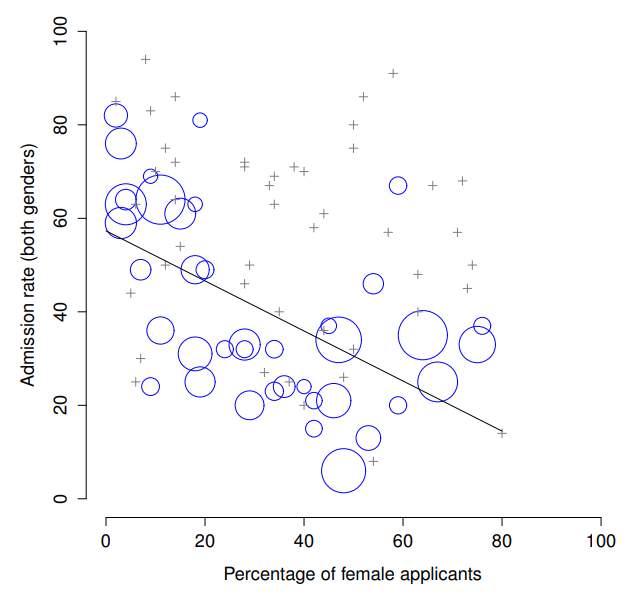
\includegraphics{./images/fig1-1.png} \hfill{}

\caption{\label{fig-fig1-1}The Berkeley 1973 college admissions data.
This figure plots the admission rate for the 85 departments that had at
least one female applicant, as a function of the percentage of
applicants that were female. The plot is a redrawing of Figure 1 from
Bickel et al. (1975). Circles plot departments with more than 40
applicants; the area of the circle is proportional to the total number
of applicants. The crosses plot departments with fewer than 40
applicants}

\end{figure}

That was the basis for my somewhat glib remarks earlier, but that's not
exactly the whole story, is it? After all, if we're interested in this
from a more sociological and psychological perspective, we might want to
ask \emph{why} there are such strong gender differences in applications.
Why do males tend to apply to engineering more often than females, and
why is this reversed for the English department? And why is it the case
that the departments that tend to have a female-application bias tend to
have lower overall admission rates than those departments that have a
male-application bias? Might this not still reflect a gender bias, even
though every single department is itself unbiased? It might. Suppose,
hypothetically, that males preferred to apply to ``hard sciences'' and
females prefer ``humanities''. And suppose further that the reason for
why the humanities departments have low admission rates is because the
government doesn't want to fund the humanities (Ph.D.~places, for
instance, are often tied to government funded research projects). Does
that constitute a gender bias? Or just an unenlightened view of the
value of the humanities? What if someone at a high level in the
government cut the humanities funds because they felt that the
humanities are ``useless chick stuff''. That seems pretty blatantly
gender biased. None of this falls within the purview of statistics, but
it matters to the research project. If you're interested in the overall
structural effects of subtle gender biases, then you probably want to
look at both the aggregated and disaggregated data. If you're interested
in the decision making process at Berkeley itself then you're probably
only interested in the disaggregated data.That was the basis for my
somewhat glib remarks earlier, but that's not exactly the whole story,
is it? After all, if we're interested in this from a more sociological
and psychological perspective, we might want to ask why there are such
strong gender differences in applications. Why do males tend to apply to
engineering more often than females, and why is this reversed for the
English department? And why is it the case that the departments that
tend to have a female-application bias tend to have lower overall
admission rates than those departments that have a male-application
bias? Might this not still reflect a gender bias, even though every
single department is itself unbiased? It might. Suppose, hypothetically,
that males preferred to apply to ``hard sciences'' and females prefer
``humanities''. And suppose further that the reason for why the
humanities departments have low admission rates is because the
government doesn't want to fund the humanities (Ph.D.~places, for
instance, are often tied to government funded research projects). Does
that constitute a gender bias? Or just an unenlightened view of the
value of the humanities? What if someone at a high level in the
government cut the humanities funds because they felt that the
humanities are ``useless chick stuff''. That seems pretty
\emph{blatantly} gender biased. None of this falls within the purview of
statistics, but it matters to the research project. If you're interested
in the overall structural effects of subtle gender biases, then you
probably want to look at \emph{both} the aggregated and disaggregated
data. If you're interested in the decision making process at Berkeley
itself then you're probably only interested in the disaggregated data.

In short there are a lot of critical questions that you can't answer
with statistics, but the answers to those questions will have a huge
impact on how you analyse and interpret data. And this is the reason why
you should always think of statistics as a tool to help you learn about
your data. No more and no less. It's a powerful tool to that end, but
there's no substitute for careful thought.

\hypertarget{statistics-in-psychology}{%
\section{Statistics in psychology}\label{statistics-in-psychology}}

I hope that the discussion above helped explain why science in general
is so focused on statistics. But I'm guessing that you have a lot more
questions about what role statistics plays in psychology, and
specifically why psychology classes always devote so many lectures to
stats. So here's my attempt to answer a few of them\ldots{}

\textbf{Why does psychology have so much statistics?}

To be perfectly honest, there's a few different reasons, some of which
are better than others. The most important reason is that psychology is
a statistical science. What I mean by that is that the ``things'' that
we study are \emph{people}. Real, complicated, gloriously messy,
infuriatingly perverse people. The ``things'' of physics include objects
like electrons, and while there are all sorts of complexities that arise
in physics, electrons don't have minds of their own. They don't have
opinions, they don't differ from each other in weird and arbitrary ways,
they don't get bored in the middle of an experiment, and they don't get
angry at the experimenter and then deliberately try to sabotage the data
set (not that I've ever done that!). At a fundamental level psychology
is harder than physics.\footnote{Which might explain why physics is just
  a teensy bit further advanced as a science than we are.} Basically, we
teach statistics to you as psychologists because you need to be better
at stats than physicists. There's actually a saying used sometimes in
physics, to the effect that ``if your experiment needs statistics, you
should have done a better experiment''. They have the luxury of being
able to say that because their objects of study are pathetically simple
in comparison to the vast mess that confronts social scientists. And
it's not just psychology. Most social sciences are desperately reliant
on statistics. Not because we're bad experimenters, but because we've
picked a harder problem to solve. We teach you stats because you really,
really need it.

\textbf{Can't someone else do the statistics?}

To some extent, but not completely. It's true that you don't need to
become a fully trained statistician just to do psychology, but you do
need to reach a certain level of statistical competence. In my view,
there's three reasons that every psychological researcher ought to be
able to do basic statistics:

\begin{itemize}
\tightlist
\item
  Firstly, there's the fundamental reason: statistics is deeply
  intertwined with research design. If you want to be good at designing
  psychological studies, you need to at the very least understand the
  basics of stats.
\item
  Secondly, if you want to be good at the psychological side of the
  research, then you need to be able to understand the psychological
  literature, right? But almost every paper in the psychological
  literature reports the results of statistical analyses. So if you
  really want to understand the psychology, you need to be able to
  understand what other people did with their data. And that means
  understanding a certain amount of statistics.
\item
  Thirdly, there's a big practical problem with being dependent on other
  people to do all your statistics: statistical analysis is
  \emph{expensive}. If you ever get bored and want to look up how much
  the Australian government charges for university fees, you'll notice
  something interesting: statistics is designated as a ``national
  priority'' category, and so the fees are much, much lower than for any
  other area of study. This is because there's a massive shortage of
  statisticians out there. So, from your perspective as a psychological
  researcher, the laws of supply and demand aren't exactly on your side
  here! As a result, in almost any real life situation where you want to
  do psychological research, the cruel facts will be that you don't have
  enough money to afford a statistician. So the economics of the
  situation mean that you have to be pretty self-sufficient.
\end{itemize}

Note that a lot of these reasons generalise beyond researchers. If you
want to be a practicing psychologist and stay on top of the field, it
helps to be able to read the scientific literature, which relies pretty
heavily on statistics.

\textbf{I don't care about jobs, research, or clinical work. Do I need
statistics?}

Okay, now you're just messing with me. Still, I think it should matter
to you too. Statistics should matter to you in the same way that
statistics should matter to \emph{everyone}. We live in the 21st
century, and data are \emph{everywhere}. Frankly, given the world in
which we live these days, a basic knowledge of statistics is pretty damn
close to a survival tool! Which is the topic of the next section.

\hypertarget{statistics-in-everyday-life}{%
\section{Statistics in everyday
life}\label{statistics-in-everyday-life}}

\begin{quote}
\emph{``We are drowning in information,\emph{\hfill\break
}but we are starved for knowledge''}\\
- Various authors, original probably John Naisbitt
\end{quote}

When I started writing up my lecture notes I took the 20 most recent
news articles posted to the ABC news website. Of those 20 articles, it
turned out that 8 of them involved a discussion of something that I
would call a statistical topic and 6 of those made a mistake. The most
common error, if you're curious, was failing to report baseline data
(e.g., the article mentions that 5\% of people in situation X have some
characteristic Y, but doesn't say how common the characteristic is for
everyone else!). The point I'm trying to make here isn't that
journalists are bad at statistics (though they almost always are), it's
that a basic knowledge of statistics is very helpful for trying to
figure out when someone else is either making a mistake or even lying to
you. In fact, one of the biggest things that a knowledge of statistics
does to you is cause you to get angry at the newspaper or the internet
on a far more frequent basis. You can find a good example of this in
Section~\ref{sec-A-real-life-example} in
Chapter~\ref{sec-Descriptive-statistics}. In later versions of this book
I'll try to include more anecdotes along those lines.

\hypertarget{theres-more-to-research-methods-than-statistics}{%
\section{There's more to research methods than
statistics}\label{theres-more-to-research-methods-than-statistics}}

So far, most of what I've talked about is statistics, and so you'd be
forgiven for thinking that statistics is all I care about in life. To be
fair, you wouldn't be far wrong, but research methodology is a broader
concept than statistics. So most research methods courses will cover a
lot of topics that relate much more to the pragmatics of research
design, and in particular the issues that you encounter when trying to
do research with humans. However, about 99\% of student fears relate to
the statistics part of the course, so I've focused on the stats in this
discussion, and hopefully I've convinced you that statistics matters,
and more importantly, that it's not to be feared. That being said, it's
pretty typical for introductory research methods classes to be very
stats-heavy. This is not (usually) because the lecturers are evil
people. Quite the contrary, in fact. Introductory classes focus a lot on
the statistics because you almost always find yourself needing
statistics before you need the other research methods training. Why?
Because almost all of your assignments in other classes will rely on
statistical training, to a much greater extent than they rely on other
methodological tools. It's not common for undergraduate assignments to
require you to design your own study from the ground up (in which case
you would need to know a lot about research design), but it \emph{is}
common for assignments to ask you to analyse and interpret data that
were collected in a study that someone else designed (in which case you
need statistics). In that sense, from the perspective of allowing you to
do well in all your other classes, the statistics is more urgent.

But note that ``urgent'' is different from ``important'' -- they both
matter. I really do want to stress that research design is just as
important as data analysis, and this book does spend a fair amount of
time on it. However, while statistics has a kind of universality, and
provides a set of core tools that are useful for most types of
psychological research, the research methods side isn't quite so
universal. There are some general principles that everyone should think
about, but a lot of research design is very idiosyncratic, and is
specific to the area of research that you want to engage in. To the
extent that it's the details that matter, those details don't usually
show up in an introductory stats and research methods class.

\hypertarget{sec-A-brief-introduction-to-research-design}{%
\chapter{A brief introduction to research
design}\label{sec-A-brief-introduction-to-research-design}}

\begin{quote}
\emph{``To consult the statistician after an experiment is finished is
often merely to ask him to conduct a post mortem examination. He can
perhaps say what the experiment died of.''}\\
-- Sir Ronald Fisher\footnote{Presidential Address to the First Indian
  Statistical Congress, 1938. Source:
  \href{http://en.wikiquote.org/wik\%0Ai/Ronald\%20Fisher}{http://en.wikiquote.org/wiki/Ronald
  Fisher}}
\end{quote}

In this chapter, we're going to start thinking about the basic ideas
that go into designing a study, collecting data, checking whether your
data collection works, and so on. It won't give you enough information
to allow you to design studies of your own, but it will give you a lot
of the basic tools that you need to assess the studies done by other
people. However, since the focus of this book is much more on data
analysis than on data collection, I'm only giving a very brief overview.
Note that this chapter is ``special'' in two ways. Firstly, it's much
more psychology specific than the later chapters. Secondly, it focuses
much more heavily on the scientific problem of research methodology, and
much less on the statistical problem of data analysis. Nevertheless, the
two problems are related to one another, so it's traditional for stats
textbooks to discuss the problem in a little detail. This chapter relies
heavily on Campbell \& Stanley (1963) and Stevens (1946) for the
discussion of scales of measurement.

\hypertarget{sec-Introduction-to-psychological-measurement}{%
\section{Introduction to psychological
measurement}\label{sec-Introduction-to-psychological-measurement}}

The first thing to understand is data collection can be thought of as a
kind of \textbf{measurement}. That is, what we're trying to do here is
measure something about human behaviour or the human mind. What do I
mean by ``measurement''?

\hypertarget{some-thoughts-about-psychological-measurement}{%
\subsection{Some thoughts about psychological
measurement}\label{some-thoughts-about-psychological-measurement}}

Measurement itself is a subtle concept, but basically it comes down to
finding some way of assigning numbers, or labels, or some other kind of
well-defined descriptions, to ``stuff''. So, any of the following would
count as a psychological measurement:

\begin{itemize}
\tightlist
\item
  My \textbf{age} is 33 years.
\item
  I do not \textbf{like anchovies.}
\item
  My \textbf{chromosomal gender} is male.
\item
  My \textbf{self-identified gender} is female.
\end{itemize}

In the short list above, the \textbf{bolded part} is ``the thing to be
measured'', and the \emph{italicised part} is ``the measurement
itself''. In fact, we can expand on this a little bit, by thinking about
the set of possible measurements that could have arisen in each case:

\begin{itemize}
\tightlist
\item
  My \textbf{age} (in years) could have been \emph{0, 1, 2, 3} \ldots,
  etc. The upper bound on what my age could possibly be is a bit fuzzy,
  but in practice you'd be safe in saying that the largest possible age
  is \emph{150}, since no human has ever lived that long.
\item
  When asked if I \textbf{like anchovies}, I might have said that
  \emph{I do, or I do not, or I have no opinion, or I sometimes do.}
\item
  My \textbf{chromosomal gender} is almost certainly going to be
  \emph{male (}\(XY\)) or \emph{female (}\(XX\)), but there are a few
  other possibilities. I could also have \emph{Klinfelter's syndrome}
  (\(XXY\)), which is more similar to male than to female. And I imagine
  there are other possibilities too.
\item
  My \textbf{self-identified} gender is also very likely to be male or
  female, but it doesn't have to agree with my chromosomal gender. I may
  also choose to identify with \emph{neither}, or to explicitly call
  myself \emph{transgender}.
\end{itemize}

As you can see, for some things (like age) it seems fairly obvious what
the set of possible measurements should be, whereas for other things it
gets a bit tricky. But I want to point out that even in the case of
someone's age it's much more subtle than this. For instance, in the
example above I assumed that it was okay to measure age in years. But if
you're a developmental psychologist, that's way too crude, and so you
often measure age in \emph{years and months} (if a child is 2 years and
11 months this is usually written as ``2;11''). If you're interested in
newborns you might want to measure age in \emph{days since birth}, maybe
even \emph{hours since birth}. In other words, the way in which you
specify the allowable measurement values is important.

Looking at this a bit more closely, you might also realise that the
concept of ``age'' isn't actually all that precise. In general, when we
say ``age'' we implicitly mean ``the length of time since birth''. But
that's not always the right way to do it. Suppose you're interested in
how newborn babies control their eye movements. If you're interested in
kids that young, you might also start to worry that ``birth'' is not the
only meaningful point in time to care about. If Baby Alice is born 3
weeks premature and Baby Bianca is born 1 week late, would it really
make sense to say that they are the ``same age'' if we encountered them
``2 hours after birth''? In one sense, yes. By social convention we use
birth as our reference point for talking about age in everyday life,
since it defines the amount of time the person has been operating as an
independent entity in the world. But from a scientific perspective
that's not the only thing we care about. When we think about the biology
of human beings, it's often useful to think of ourselves as organisms
that have been growing and maturing since conception, and from that
perspective Alice and Bianca aren't the same age at all. So you might
want to define the concept of ``age'' in two different ways: the length
of time since conception and the length of time since birth. When
dealing with adults it won't make much difference, but when dealing with
newborns it might.

Moving beyond these issues, there's the question of methodology. What
specific ``measurement method'' are you going to use to find out
someone's age? As before, there are lots of different possibilities:

\begin{itemize}
\tightlist
\item
  You could just ask people ``how old are you?'' The method of
  self-report is fast, cheap and easy. But it only works with people old
  enough to understand the question, and some people lie about their
  age.
\item
  You could ask an authority (e.g., a parent) ``how old is your child?''
  This method is fast, and when dealing with kids it's not all that hard
  since the parent is almost always around. It doesn't work as well if
  you want to know ``age since conception'', since a lot of parents
  can't say for sure when conception took place. For that, you might
  need a different authority (e.g., an obstetrician).
\item
  You could look up official records, for example birth or death
  certificates. This is a time consuming and frustrating endeavour, but
  it has its uses (e.g., if the person is now dead).
\end{itemize}

\hypertarget{operationalisation-defining-your-measurement}{%
\subsection{Operationalisation: defining your
measurement}\label{operationalisation-defining-your-measurement}}

All of the ideas discussed in the previous section relate to the concept
of \textbf{operationalisation}. To be a bit more precise about the idea,
operationalisation is the process by which we take a meaningful but
somewhat vague concept and turn it into a precise measurement. The
process of operationalisation can involve several different things:

\begin{itemize}
\item
  Being precise about what you are trying to measure. For instance, does
  ``age'' mean ``time since birth'' or ``time since conception'' in the
  context of your research?
\item
  Determining what method you will use to measure it. Will you use
  self-report to measure age, ask a parent, or look up an official
  record? If you're using self-report, how will you phrase the question?
\item
  Defining the set of allowable values that the measurement can take.
  Note that these values don't always have to be numerical, though they
  often are. When measuring age the values are numerical, but we still
  need to think carefully about what numbers are allowed. Do we want age
  in years, years and months, days, or hours? For other types of
  measurements (e.g., gender) the values aren't numerical. But, just as
  before, we need to think about what values are allowed. If we're
  asking people to self-report their gender, what options to we allow
  them to choose between? Is it enough to allow only ``male'' or
  ``female''? Do you need an ``other'' option? Or should we not give
  people specific options and instead let them answer in their own
  words? And if you open up the set of possible values to include all
  verbal response, how will you interpret their answers?
\end{itemize}

Operationalisation is a tricky business, and there's no ``one, true
way'' to do it. The way in which you choose to operationalise the
informal concept of ``age'' or ``gender'' into a formal measurement
depends on what you need to use the measurement for. Often you'll find
that the community of scientists who work in your area have some fairly
well-established ideas for how to go about it. In other words,
operationalisation needs to be thought through on a case by case basis.
Nevertheless, while there a lot of issues that are specific to each
individual research project, there are some aspects to it that are
pretty general.

Before moving on I want to take a moment to clear up our terminology,
and in the process introduce one more term. Here are four different
things that are closely related to each other:

\begin{itemize}
\tightlist
\item
  \textbf{A theoretical construct.} This is the thing that you're trying
  to take a measurement of, like ``age'', ``gender'' or an ``opinion''.
  A theoretical construct can't be directly observed, and often they're
  actually a bit vague.
\item
  \textbf{A measure.} The measure refers to the method or the tool that
  you use to make your observations. A question in a survey, a
  behavioural observation or a brain scan could all count as a measure.
\item
  \textbf{An operationalisation.} The term ``operationalisation'' refers
  to the logical connection between the measure and the theoretical
  construct, or to the process by which we try to derive a measure from
  a theoretical construct.
\item
  \textbf{A variable.} Finally, a new term. A variable is what we end up
  with when we apply our measure to something in the world. That is,
  variables are the actual ``data'' that we end up with in our data
  sets.
\end{itemize}

In practice, even scientists tend to blur the distinction between these
things, but it's very helpful to try to understand the differences.

\hypertarget{sec-Scales-of-measurement}{%
\section{Scales of measurement}\label{sec-Scales-of-measurement}}

As the previous section indicates, the outcome of a psychological
measurement is called a variable. But not all variables are of the same
qualitative type and so it's useful to understand what types there are.
A very useful concept for distinguishing between different types of
variables is what's known as \textbf{scales of measurement}.

\hypertarget{nominal-scale}{%
\subsection{Nominal scale}\label{nominal-scale}}

A \textbf{nominal scale} variable (also referred to as a
\textbf{categorical} variable) is one in which there is no particular
relationship between the different possibilities. For these kinds of
variables it doesn't make any sense to say that one of them is ``bigger'
or''better'' than any other one, and it absolutely doesn't make any
sense to average them. The classic example for this is ``eye colour''.
Eyes can be blue, green or brown, amongst other possibilities, but none
of them is any ``bigger'' than any other one. As a result, it would feel
really weird to talk about an ``average eye colour''. Similarly, gender
is nominal too: male isn't better or worse than female. Neither does it
make sense to try to talk about an ``average gender''. In short, nominal
scale variables are those for which the only thing you can say about the
different possibilities is that they are different. That's it.

Let's take a slightly closer look at this. Suppose I was doing research
on how people commute to and from work. One variable I would have to
measure would be what kind of transportation people use to get to work.
This ``transport type'' variable could have quite a few possible values,
including: ``train'', ``bus'', ``car'', ``bicycle''. For now, let's
suppose that these four are the only possibilities. Then imagine that I
ask 100 people how they got to work today, with this result
(Table~\ref{tbl-tab2-1}).

\hypertarget{tbl-tab2-1}{}
 
  \providecommand{\huxb}[2]{\arrayrulecolor[RGB]{#1}\global\arrayrulewidth=#2pt}
  \providecommand{\huxvb}[2]{\color[RGB]{#1}\vrule width #2pt}
  \providecommand{\huxtpad}[1]{\rule{0pt}{#1}}
  \providecommand{\huxbpad}[1]{\rule[-#1]{0pt}{#1}}

\begin{table}[ht]
\caption{\label{tbl-tab2-1}How did 100 people get to work today }\tabularnewline

\begin{centerbox}
\begin{threeparttable}
\setlength{\tabcolsep}{0pt}
\begin{tabularx}{0.9\textwidth}{p{0.45\textwidth} p{0.45\textwidth}}


\hhline{>{\huxb{0, 0, 0}{0.4}}->{\huxb{0, 0, 0}{0.4}}-}
\arrayrulecolor{black}

\multicolumn{1}{!{\huxvb{0, 0, 0}{0}}p{0.45\textwidth}!{\huxvb{0, 0, 0}{0}}}{\cellcolor[RGB]{242, 242, 242}\hspace{0pt}\parbox[b]{0.45\textwidth-0pt-6pt}{\huxtpad{6pt + 1em}\centering \textbf{Transportation}\huxbpad{6pt}}} &
\multicolumn{1}{p{0.45\textwidth}!{\huxvb{0, 0, 0}{0}}}{\cellcolor[RGB]{242, 242, 242}\hspace{6pt}\parbox[b]{0.45\textwidth-6pt-0pt}{\huxtpad{6pt + 1em}\centering \textbf{Number of people}\huxbpad{6pt}}} \tabularnewline[-0.5pt]


\hhline{>{\huxb{0, 0, 0}{0.4}}->{\huxb{0, 0, 0}{0.4}}-}
\arrayrulecolor{black}

\multicolumn{1}{!{\huxvb{0, 0, 0}{0}}p{0.45\textwidth}!{\huxvb{0, 0, 0}{0}}}{\hspace{0pt}\parbox[b]{0.45\textwidth-0pt-6pt}{\huxtpad{6pt + 1em}\centering (1) Train\huxbpad{6pt}}} &
\multicolumn{1}{p{0.45\textwidth}!{\huxvb{0, 0, 0}{0}}}{\hspace{6pt}\parbox[b]{0.45\textwidth-6pt-0pt}{\huxtpad{6pt + 1em}\centering 12\huxbpad{6pt}}} \tabularnewline[-0.5pt]


\hhline{}
\arrayrulecolor{black}

\multicolumn{1}{!{\huxvb{0, 0, 0}{0}}p{0.45\textwidth}!{\huxvb{0, 0, 0}{0}}}{\cellcolor[RGB]{242, 242, 242}\hspace{0pt}\parbox[b]{0.45\textwidth-0pt-6pt}{\huxtpad{6pt + 1em}\centering (2) Bus\huxbpad{6pt}}} &
\multicolumn{1}{p{0.45\textwidth}!{\huxvb{0, 0, 0}{0}}}{\cellcolor[RGB]{242, 242, 242}\hspace{6pt}\parbox[b]{0.45\textwidth-6pt-0pt}{\huxtpad{6pt + 1em}\centering 30\huxbpad{6pt}}} \tabularnewline[-0.5pt]


\hhline{}
\arrayrulecolor{black}

\multicolumn{1}{!{\huxvb{0, 0, 0}{0}}p{0.45\textwidth}!{\huxvb{0, 0, 0}{0}}}{\hspace{0pt}\parbox[b]{0.45\textwidth-0pt-6pt}{\huxtpad{6pt + 1em}\centering (3) Car\huxbpad{6pt}}} &
\multicolumn{1}{p{0.45\textwidth}!{\huxvb{0, 0, 0}{0}}}{\hspace{6pt}\parbox[b]{0.45\textwidth-6pt-0pt}{\huxtpad{6pt + 1em}\centering 48\huxbpad{6pt}}} \tabularnewline[-0.5pt]


\hhline{}
\arrayrulecolor{black}

\multicolumn{1}{!{\huxvb{0, 0, 0}{0}}p{0.45\textwidth}!{\huxvb{0, 0, 0}{0}}}{\cellcolor[RGB]{242, 242, 242}\hspace{0pt}\parbox[b]{0.45\textwidth-0pt-6pt}{\huxtpad{6pt + 1em}\centering (4) Bicycle\huxbpad{6pt}}} &
\multicolumn{1}{p{0.45\textwidth}!{\huxvb{0, 0, 0}{0}}}{\cellcolor[RGB]{242, 242, 242}\hspace{6pt}\parbox[b]{0.45\textwidth-6pt-0pt}{\huxtpad{6pt + 1em}\centering 10\huxbpad{6pt}}} \tabularnewline[-0.5pt]


\hhline{>{\huxb{0, 0, 0}{0.4}}->{\huxb{0, 0, 0}{0.4}}-}
\arrayrulecolor{black}
\end{tabularx} 

\end{threeparttable}\par\end{centerbox}

\end{table}
 

So, what's the average transportation type? Obviously, the answer here
is that there isn't one. It's a silly question to ask. You can say that
travel by car is the most popular method, and travel by train is the
least popular method, but that's about all. Similarly, notice that the
order in which I list the options isn't very interesting. I could have
chosen to display the data like in Table~\ref{tbl-tab2-2}.

\hypertarget{tbl-tab2-2}{}
 
  \providecommand{\huxb}[2]{\arrayrulecolor[RGB]{#1}\global\arrayrulewidth=#2pt}
  \providecommand{\huxvb}[2]{\color[RGB]{#1}\vrule width #2pt}
  \providecommand{\huxtpad}[1]{\rule{0pt}{#1}}
  \providecommand{\huxbpad}[1]{\rule[-#1]{0pt}{#1}}

\begin{table}[ht]
\caption{\label{tbl-tab2-2}How did 100 people get to work today, a different view }\tabularnewline

\begin{centerbox}
\begin{threeparttable}
\setlength{\tabcolsep}{0pt}
\begin{tabularx}{0.9\textwidth}{p{0.45\textwidth} p{0.45\textwidth}}


\hhline{>{\huxb{0, 0, 0}{0.4}}->{\huxb{0, 0, 0}{0.4}}-}
\arrayrulecolor{black}

\multicolumn{1}{!{\huxvb{0, 0, 0}{0}}p{0.45\textwidth}!{\huxvb{0, 0, 0}{0}}}{\cellcolor[RGB]{242, 242, 242}\hspace{0pt}\parbox[b]{0.45\textwidth-0pt-6pt}{\huxtpad{6pt + 1em}\centering \textbf{Transportation}\huxbpad{6pt}}} &
\multicolumn{1}{p{0.45\textwidth}!{\huxvb{0, 0, 0}{0}}}{\cellcolor[RGB]{242, 242, 242}\hspace{6pt}\parbox[b]{0.45\textwidth-6pt-0pt}{\huxtpad{6pt + 1em}\centering \textbf{Number of people}\huxbpad{6pt}}} \tabularnewline[-0.5pt]


\hhline{>{\huxb{0, 0, 0}{0.4}}->{\huxb{0, 0, 0}{0.4}}-}
\arrayrulecolor{black}

\multicolumn{1}{!{\huxvb{0, 0, 0}{0}}p{0.45\textwidth}!{\huxvb{0, 0, 0}{0}}}{\hspace{0pt}\parbox[b]{0.45\textwidth-0pt-6pt}{\huxtpad{6pt + 1em}\centering (3) Car\huxbpad{6pt}}} &
\multicolumn{1}{p{0.45\textwidth}!{\huxvb{0, 0, 0}{0}}}{\hspace{6pt}\parbox[b]{0.45\textwidth-6pt-0pt}{\huxtpad{6pt + 1em}\centering 48\huxbpad{6pt}}} \tabularnewline[-0.5pt]


\hhline{}
\arrayrulecolor{black}

\multicolumn{1}{!{\huxvb{0, 0, 0}{0}}p{0.45\textwidth}!{\huxvb{0, 0, 0}{0}}}{\cellcolor[RGB]{242, 242, 242}\hspace{0pt}\parbox[b]{0.45\textwidth-0pt-6pt}{\huxtpad{6pt + 1em}\centering (1) Train\huxbpad{6pt}}} &
\multicolumn{1}{p{0.45\textwidth}!{\huxvb{0, 0, 0}{0}}}{\cellcolor[RGB]{242, 242, 242}\hspace{6pt}\parbox[b]{0.45\textwidth-6pt-0pt}{\huxtpad{6pt + 1em}\centering 12\huxbpad{6pt}}} \tabularnewline[-0.5pt]


\hhline{}
\arrayrulecolor{black}

\multicolumn{1}{!{\huxvb{0, 0, 0}{0}}p{0.45\textwidth}!{\huxvb{0, 0, 0}{0}}}{\hspace{0pt}\parbox[b]{0.45\textwidth-0pt-6pt}{\huxtpad{6pt + 1em}\centering (4) Bicycle\huxbpad{6pt}}} &
\multicolumn{1}{p{0.45\textwidth}!{\huxvb{0, 0, 0}{0}}}{\hspace{6pt}\parbox[b]{0.45\textwidth-6pt-0pt}{\huxtpad{6pt + 1em}\centering 10\huxbpad{6pt}}} \tabularnewline[-0.5pt]


\hhline{}
\arrayrulecolor{black}

\multicolumn{1}{!{\huxvb{0, 0, 0}{0}}p{0.45\textwidth}!{\huxvb{0, 0, 0}{0}}}{\cellcolor[RGB]{242, 242, 242}\hspace{0pt}\parbox[b]{0.45\textwidth-0pt-6pt}{\huxtpad{6pt + 1em}\centering (2) Bus\huxbpad{6pt}}} &
\multicolumn{1}{p{0.45\textwidth}!{\huxvb{0, 0, 0}{0}}}{\cellcolor[RGB]{242, 242, 242}\hspace{6pt}\parbox[b]{0.45\textwidth-6pt-0pt}{\huxtpad{6pt + 1em}\centering 30\huxbpad{6pt}}} \tabularnewline[-0.5pt]


\hhline{>{\huxb{0, 0, 0}{0.4}}->{\huxb{0, 0, 0}{0.4}}-}
\arrayrulecolor{black}
\end{tabularx} 

\end{threeparttable}\par\end{centerbox}

\end{table}
 

\ldots and nothing really changes.

\hypertarget{ordinal-scale}{%
\subsection{Ordinal scale}\label{ordinal-scale}}

\textbf{Ordinal scale} variables have a bit more structure than nominal
scale variables, but not by a lot. An ordinal scale variable is one in
which there is a natural, meaningful way to order the different
possibilities, but you can't do anything else. The usual example given
of an ordinal variable is ``finishing position in a race''. You
\emph{can} say that the person who finished first was faster than the
person who finished second, but you \emph{don't} know how much faster.
As a consequence we know that 1st \(>\) 2nd, and we know that 2nd \(>\)
3rd, but the difference between 1st and 2nd might be much larger than
the difference between 2nd and 3rd.

Here's a more psychologically interesting example. Suppose I'm
interested in people's attitudes to climate change. I then go and ask
some people to pick the statement (from four listed statements) that
most closely matches their beliefs:

\begin{enumerate}
\def\labelenumi{\arabic{enumi}.}
\tightlist
\item
  Temperatures are rising because of human activity
\item
  Temperatures are rising but we don't know why
\item
  Temperatures are rising but not because of humans
\item
  Temperatures are not rising
\end{enumerate}

Notice that these four statements actually do have a natural ordering,
in terms of ``the extent to which they agree with the current science''.
Statement 1 is a close match, statement 2 is a reasonable match,
statement 3 isn't a very good match, and statement 4 is in strong
opposition to current science. So, in terms of the thing I'm interested
in (the extent to which people endorse the science), I can order the
items as 1 \(>\) 2 \(>\) 3 \(>\) 4. Since this ordering exists, it would
be very weird to list the options like this\ldots{}

\begin{enumerate}
\def\labelenumi{\arabic{enumi}.}
\tightlist
\item
  Temperatures are rising but not because of humans
\item
  Temperatures are rising because of human activity
\item
  Temperatures are not rising
\item
  Temperatures are rising but we don't know why
\end{enumerate}

\ldots because it seems to violate the natural ``structure'' to the
question.

So, let's suppose I asked 100 people these questions, and got the
answers shown in Table~\ref{tbl-tab2-3}.

\hypertarget{tbl-tab2-3}{}
 
  \providecommand{\huxb}[2]{\arrayrulecolor[RGB]{#1}\global\arrayrulewidth=#2pt}
  \providecommand{\huxvb}[2]{\color[RGB]{#1}\vrule width #2pt}
  \providecommand{\huxtpad}[1]{\rule{0pt}{#1}}
  \providecommand{\huxbpad}[1]{\rule[-#1]{0pt}{#1}}

\begin{table}[ht]
\caption{\label{tbl-tab2-3}Attitudes to climate change }\tabularnewline

\begin{centerbox}
\begin{threeparttable}
\setlength{\tabcolsep}{0pt}
\begin{tabularx}{0.9\textwidth}{p{0.45\textwidth} p{0.45\textwidth}}


\hhline{>{\huxb{0, 0, 0}{0.4}}->{\huxb{0, 0, 0}{0.4}}-}
\arrayrulecolor{black}

\multicolumn{1}{!{\huxvb{0, 0, 0}{0}}p{0.45\textwidth}!{\huxvb{0, 0, 0}{0}}}{\cellcolor[RGB]{242, 242, 242}\hspace{0pt}\parbox[b]{0.45\textwidth-0pt-6pt}{\huxtpad{6pt + 1em}\centering \textbf{Response}\huxbpad{6pt}}} &
\multicolumn{1}{p{0.45\textwidth}!{\huxvb{0, 0, 0}{0}}}{\cellcolor[RGB]{242, 242, 242}\hspace{6pt}\parbox[b]{0.45\textwidth-6pt-0pt}{\huxtpad{6pt + 1em}\centering \textbf{Number}\huxbpad{6pt}}} \tabularnewline[-0.5pt]


\hhline{>{\huxb{0, 0, 0}{0.4}}->{\huxb{0, 0, 0}{0.4}}-}
\arrayrulecolor{black}

\multicolumn{1}{!{\huxvb{0, 0, 0}{0}}p{0.45\textwidth}!{\huxvb{0, 0, 0}{0}}}{\hspace{0pt}\parbox[b]{0.45\textwidth-0pt-6pt}{\huxtpad{6pt + 1em}\centering (1) Temperatures are rising because of human activity\huxbpad{6pt}}} &
\multicolumn{1}{p{0.45\textwidth}!{\huxvb{0, 0, 0}{0}}}{\hspace{6pt}\parbox[b]{0.45\textwidth-6pt-0pt}{\huxtpad{6pt + 1em}\centering 51\huxbpad{6pt}}} \tabularnewline[-0.5pt]


\hhline{}
\arrayrulecolor{black}

\multicolumn{1}{!{\huxvb{0, 0, 0}{0}}p{0.45\textwidth}!{\huxvb{0, 0, 0}{0}}}{\cellcolor[RGB]{242, 242, 242}\hspace{0pt}\parbox[b]{0.45\textwidth-0pt-6pt}{\huxtpad{6pt + 1em}\centering (2) Temperatures are rising but we don’t know why\huxbpad{6pt}}} &
\multicolumn{1}{p{0.45\textwidth}!{\huxvb{0, 0, 0}{0}}}{\cellcolor[RGB]{242, 242, 242}\hspace{6pt}\parbox[b]{0.45\textwidth-6pt-0pt}{\huxtpad{6pt + 1em}\centering 20\huxbpad{6pt}}} \tabularnewline[-0.5pt]


\hhline{}
\arrayrulecolor{black}

\multicolumn{1}{!{\huxvb{0, 0, 0}{0}}p{0.45\textwidth}!{\huxvb{0, 0, 0}{0}}}{\hspace{0pt}\parbox[b]{0.45\textwidth-0pt-6pt}{\huxtpad{6pt + 1em}\centering (3) Temperatures are rising but not because of humans\huxbpad{6pt}}} &
\multicolumn{1}{p{0.45\textwidth}!{\huxvb{0, 0, 0}{0}}}{\hspace{6pt}\parbox[b]{0.45\textwidth-6pt-0pt}{\huxtpad{6pt + 1em}\centering 10\huxbpad{6pt}}} \tabularnewline[-0.5pt]


\hhline{}
\arrayrulecolor{black}

\multicolumn{1}{!{\huxvb{0, 0, 0}{0}}p{0.45\textwidth}!{\huxvb{0, 0, 0}{0}}}{\cellcolor[RGB]{242, 242, 242}\hspace{0pt}\parbox[b]{0.45\textwidth-0pt-6pt}{\huxtpad{6pt + 1em}\centering (4) Temperatures are not rising\huxbpad{6pt}}} &
\multicolumn{1}{p{0.45\textwidth}!{\huxvb{0, 0, 0}{0}}}{\cellcolor[RGB]{242, 242, 242}\hspace{6pt}\parbox[b]{0.45\textwidth-6pt-0pt}{\huxtpad{6pt + 1em}\centering 19\huxbpad{6pt}}} \tabularnewline[-0.5pt]


\hhline{>{\huxb{0, 0, 0}{0.4}}->{\huxb{0, 0, 0}{0.4}}-}
\arrayrulecolor{black}
\end{tabularx} 

\end{threeparttable}\par\end{centerbox}

\end{table}
 

When analysing these data it seems quite reasonable to try to group (1),
(2) and (3) together, and say that 81 out of 100 people were willing to
at \emph{least partially} endorse the science. And it's also quite
reasonable to group (2), (3) and (4) together and say that 49 out of 100
people registered \emph{at least some disagreement} with the dominant
scientific view. However, it would be entirely bizarre to try to group
(1), (2) and (4) together and say that 90 out of 100 people said\ldots{}
what? There's nothing sensible that allows you to group those responses
together at all.

That said, notice that while we \emph{can} use the natural ordering of
these items to construct sensible groupings, what we can't do is average
them. For instance, in my simple example here, the ``average'' response
to the question is 1.97. If you can tell me what that means I'd love to
know, because it seems like gibberish to me!

\hypertarget{interval-scale}{%
\subsection{Interval scale}\label{interval-scale}}

In contrast to nominal and ordinal scale variables, \textbf{interval
scale} and ratio scale variables are variables for which the numerical
value is genuinely meaningful. In the case of interval scale variables
the \emph{differences} between the numbers are interpretable, but the
variable doesn't have a ``natural'' zero value. A good example of an
interval scale variable is measuring temperature in degrees celsius. For
instance, if it was 15\(^{\circ}\) yesterday and 18\(^{\circ}\) today,
then the 3\(^{\circ}\) difference between the two is genuinely
meaningful. Moreover, that 3\(^{\circ}\) difference is \emph{exactly the
same} as the 3\(^{\circ}\) difference between 7\(^{\circ}\) and
10\(^{\circ}\). In short, addition and subtraction are meaningful for
interval scale variables.\footnote{Actually, I've been informed by
  readers with greater physics knowledge than I that temperature isn't
  strictly an interval scale, in the sense that the amount of energy
  required to heat something up by 3° depends on it's current
  temperature. So in the sense that physicists care about, temperature
  isn't actually an interval scale. But it still makes a cute example so
  I'm going to ignore this little inconvenient truth.}

However, notice that the 0\(^{\circ}\) does not mean ``no temperature at
all''. It actually means ``the temperature at which water freezes'',
which is pretty arbitrary. As a consequence it becomes pointless to try
to multiply and divide temperatures. It is wrong to say that
20\(^{\circ}\) is twice as hot as 10\(^{\circ}\), just as it is weird
and meaningless to try to claim that 20\(^{\circ}\) is negative two
times as hot as -10\(^{\circ}\).

Again, lets look at a more psychological example. Suppose I'm interested
in looking at how the attitudes of first-year university students have
changed over time. Obviously, I'm going to want to record the year in
which each student started. This is an interval scale variable. A
student who started in 2003 did arrive 5 years before a student who
started in 2008. However, it would be completely daft for me to divide
2008 by 2003 and say that the second student started ``1.0024 times
later'' than the first one. That doesn't make any sense at all.

\hypertarget{ratio-scale}{%
\subsection{Ratio scale}\label{ratio-scale}}

The fourth and final type of variable to consider is a \textbf{ratio
scale} variable, in which zero really means zero, and it's okay to
multiply and divide. A good psychological example of a ratio scale
variable is response time (RT). In a lot of tasks it's very common to
record the amount of time somebody takes to solve a problem or answer a
question, because it's an indicator of how difficult the task is.
Suppose that Alan takes 2.3 seconds to respond to a question, whereas
Ben takes 3.1 seconds. As with an interval scale variable, addition and
subtraction are both meaningful here. Ben really did take 3.1 - 2.3 =
0.8 seconds longer than Alan did. However, notice that multiplication
and division also make sense here too: Ben took 3.1/2.3 = 1.35 times as
long as Alan did to answer the question. And the reason why you can do
this is that for a ratio scale variable such as RT ``zero seconds''
really does mean ``no time at all''.

\hypertarget{continuous-versus-discrete-variables}{%
\subsection{Continuous versus discrete
variables}\label{continuous-versus-discrete-variables}}

There's a second kind of distinction that you need to be aware of,
regarding what types of variables you can run into. This is the
distinction between continuous variables and discrete variables
(Table~\ref{tbl-tab2-4}). The difference between these is as follows:

\begin{itemize}
\tightlist
\item
  A \textbf{continuous variable} is one in which, for any two values
  that you can think of, it's always logically possible to have another
  value in between.
\item
  A \textbf{discrete variable} is, in effect, a variable that isn't
  continuous. For a discrete variable it's sometimes the case that
  there's nothing in the middle.
\end{itemize}

\hypertarget{tbl-tab2-4}{}
 
  \providecommand{\huxb}[2]{\arrayrulecolor[RGB]{#1}\global\arrayrulewidth=#2pt}
  \providecommand{\huxvb}[2]{\color[RGB]{#1}\vrule width #2pt}
  \providecommand{\huxtpad}[1]{\rule{0pt}{#1}}
  \providecommand{\huxbpad}[1]{\rule[-#1]{0pt}{#1}}

\begin{table}[ht]
\caption{\label{tbl-tab2-4}The relationship between the scales of measurement and the
discrete/continuity distinction. Cells with a tick mark correspond to
things that are possible }\tabularnewline

\begin{centerbox}
\begin{threeparttable}
\setlength{\tabcolsep}{0pt}
\begin{tabularx}{0.9\textwidth}{p{0.3\textwidth} p{0.3\textwidth} p{0.3\textwidth}}


\hhline{>{\huxb{0, 0, 0}{0.4}}->{\huxb{0, 0, 0}{0.4}}->{\huxb{0, 0, 0}{0.4}}-}
\arrayrulecolor{black}

\multicolumn{1}{!{\huxvb{0, 0, 0}{0}}p{0.3\textwidth}!{\huxvb{0, 0, 0}{0}}}{\cellcolor[RGB]{242, 242, 242}\hspace{0pt}\parbox[b]{0.3\textwidth-0pt-6pt}{\huxtpad{6pt + 1em}\centering \textbf{}\huxbpad{6pt}}} &
\multicolumn{1}{p{0.3\textwidth}!{\huxvb{0, 0, 0}{0}}}{\cellcolor[RGB]{242, 242, 242}\hspace{6pt}\parbox[b]{0.3\textwidth-6pt-6pt}{\huxtpad{6pt + 1em}\centering \textbf{continuous}\huxbpad{6pt}}} &
\multicolumn{1}{p{0.3\textwidth}!{\huxvb{0, 0, 0}{0}}}{\cellcolor[RGB]{242, 242, 242}\hspace{6pt}\parbox[b]{0.3\textwidth-6pt-0pt}{\huxtpad{6pt + 1em}\centering \textbf{discrete}\huxbpad{6pt}}} \tabularnewline[-0.5pt]


\hhline{>{\huxb{0, 0, 0}{0.4}}->{\huxb{0, 0, 0}{0.4}}->{\huxb{0, 0, 0}{0.4}}-}
\arrayrulecolor{black}

\multicolumn{1}{!{\huxvb{0, 0, 0}{0}}p{0.3\textwidth}!{\huxvb{0, 0, 0}{0}}}{\hspace{0pt}\parbox[b]{0.3\textwidth-0pt-6pt}{\huxtpad{6pt + 1em}\centering nominal\huxbpad{6pt}}} &
\multicolumn{1}{p{0.3\textwidth}!{\huxvb{0, 0, 0}{0}}}{\hspace{6pt}\parbox[b]{0.3\textwidth-6pt-6pt}{\huxtpad{6pt + 1em}\centering \huxbpad{6pt}}} &
\multicolumn{1}{p{0.3\textwidth}!{\huxvb{0, 0, 0}{0}}}{\hspace{6pt}\parbox[b]{0.3\textwidth-6pt-0pt}{\huxtpad{6pt + 1em}\centering \( \checkmark \)\huxbpad{6pt}}} \tabularnewline[-0.5pt]


\hhline{}
\arrayrulecolor{black}

\multicolumn{1}{!{\huxvb{0, 0, 0}{0}}p{0.3\textwidth}!{\huxvb{0, 0, 0}{0}}}{\cellcolor[RGB]{242, 242, 242}\hspace{0pt}\parbox[b]{0.3\textwidth-0pt-6pt}{\huxtpad{6pt + 1em}\centering ordinal\huxbpad{6pt}}} &
\multicolumn{1}{p{0.3\textwidth}!{\huxvb{0, 0, 0}{0}}}{\cellcolor[RGB]{242, 242, 242}\hspace{6pt}\parbox[b]{0.3\textwidth-6pt-6pt}{\huxtpad{6pt + 1em}\centering \huxbpad{6pt}}} &
\multicolumn{1}{p{0.3\textwidth}!{\huxvb{0, 0, 0}{0}}}{\cellcolor[RGB]{242, 242, 242}\hspace{6pt}\parbox[b]{0.3\textwidth-6pt-0pt}{\huxtpad{6pt + 1em}\centering \( \checkmark \)\huxbpad{6pt}}} \tabularnewline[-0.5pt]


\hhline{}
\arrayrulecolor{black}

\multicolumn{1}{!{\huxvb{0, 0, 0}{0}}p{0.3\textwidth}!{\huxvb{0, 0, 0}{0}}}{\hspace{0pt}\parbox[b]{0.3\textwidth-0pt-6pt}{\huxtpad{6pt + 1em}\centering interval\huxbpad{6pt}}} &
\multicolumn{1}{p{0.3\textwidth}!{\huxvb{0, 0, 0}{0}}}{\hspace{6pt}\parbox[b]{0.3\textwidth-6pt-6pt}{\huxtpad{6pt + 1em}\centering \( \checkmark \)\huxbpad{6pt}}} &
\multicolumn{1}{p{0.3\textwidth}!{\huxvb{0, 0, 0}{0}}}{\hspace{6pt}\parbox[b]{0.3\textwidth-6pt-0pt}{\huxtpad{6pt + 1em}\centering \( \checkmark \)\huxbpad{6pt}}} \tabularnewline[-0.5pt]


\hhline{}
\arrayrulecolor{black}

\multicolumn{1}{!{\huxvb{0, 0, 0}{0}}p{0.3\textwidth}!{\huxvb{0, 0, 0}{0}}}{\cellcolor[RGB]{242, 242, 242}\hspace{0pt}\parbox[b]{0.3\textwidth-0pt-6pt}{\huxtpad{6pt + 1em}\centering ratio\huxbpad{6pt}}} &
\multicolumn{1}{p{0.3\textwidth}!{\huxvb{0, 0, 0}{0}}}{\cellcolor[RGB]{242, 242, 242}\hspace{6pt}\parbox[b]{0.3\textwidth-6pt-6pt}{\huxtpad{6pt + 1em}\centering \( \checkmark \)\huxbpad{6pt}}} &
\multicolumn{1}{p{0.3\textwidth}!{\huxvb{0, 0, 0}{0}}}{\cellcolor[RGB]{242, 242, 242}\hspace{6pt}\parbox[b]{0.3\textwidth-6pt-0pt}{\huxtpad{6pt + 1em}\centering \( \checkmark \)\huxbpad{6pt}}} \tabularnewline[-0.5pt]


\hhline{>{\huxb{0, 0, 0}{0.4}}->{\huxb{0, 0, 0}{0.4}}->{\huxb{0, 0, 0}{0.4}}-}
\arrayrulecolor{black}
\end{tabularx} 

\end{threeparttable}\par\end{centerbox}

\end{table}
 

These definitions probably seem a bit abstract, but they're pretty
simple once you see some examples. For instance, response time is
continuous. If Alan takes 3.1 seconds and Ben takes 2.3 seconds to
respond to a question, then Cameron's response time will lie in between
if he took 3.0 seconds. And of course it would also be possible for
David to take 3.031 seconds to respond, meaning that his RT would lie in
between Cameron's and Alan's. And while in practice it might be
impossible to measure RT that precisely, it's certainly possible in
principle. Because we can always find a new value for RT in between any
two other ones we regard RT as a continuous measure.

Discrete variables occur when this rule is violated. For example,
nominal scale variables are always discrete. There isn't a type of
transportation that falls ``in between'' trains and bicycles, not in the
strict mathematical way that 2.3 falls in between 2 and 3. So
transportation type is discrete. Similarly, ordinal scale variables are
always discrete. Although ``2nd place'' does fall between ``1st place''
and ``3rd place'', there's nothing that can logically fall in between
``1st place'' and ``2nd place''. Interval scale and ratio scale
variables can go either way. As we saw above, response time (a ratio
scale variable) is continuous. Temperature in degrees celsius (an
interval scale variable) is also continuous. However, the year you went
to school (an interval scale variable) is discrete. There's no year in
between 2002 and 2003. The number of questions you get right on a
true-or-false test (a ratio scale variable) is also discrete. Since a
true-or-false question doesn't allow you to be ``partially correct'',
there's nothing in between 5/10 and 6/10. Table~\ref{tbl-tab2-4}
summarises the relationship between the scales of measurement and the
discrete/continuity distinction. Cells with a tick mark correspond to
things that are possible. I'm trying to hammer this point home, because
(a) some textbooks get this wrong, and (b) people very often say things
like ``discrete variable'' when they mean ``nominal scale variable''.
It's very unfortunate.

\hypertarget{some-complexities}{%
\subsection{Some complexities}\label{some-complexities}}

Okay, I know you're going to be shocked to hear this, but the real world
is much messier than this little classification scheme suggests. Very
few variables in real life actually fall into these nice neat
categories, so you need to be kind of careful not to treat the scales of
measurement as if they were hard and fast rules. It doesn't work like
that. They're guidelines, intended to help you think about the
situations in which you should treat different variables differently.
Nothing more.

So let's take a classic example, maybe \emph{the} classic example, of a
psychological measurement tool: the \textbf{Likert scale}. The humble
Likert scale is the bread and butter tool of all survey design. You
yourself have filled out hundreds, maybe thousands, of them and odds are
you've even used one yourself. Suppose we have a survey question that
looks like this:

Which of the following best describes your opinion of the statement that
``all pirates are freaking awesome''?

and then the options presented to the participant are these:

\begin{enumerate}
\def\labelenumi{\arabic{enumi}.}
\tightlist
\item
  Strongly disagree
\item
  Disagree
\item
  Neither agree nor disagree
\item
  Agree
\item
  Strongly agree
\end{enumerate}

This set of items is an example of a 5-point Likert scale, in which
people are asked to choose among one of several (in this case 5) clearly
ordered possibilities, generally with a verbal descriptor given in each
case. However, it's not necessary that all items are explicitly
described. This is a perfectly good example of a 5-point Likert scale
too:

\begin{enumerate}
\def\labelenumi{\arabic{enumi}.}
\tightlist
\item
  Strongly disagree
\item
\item
\item
\item
  Strongly agree
\end{enumerate}

Likert scales are very handy, if somewhat limited, tools. The question
is what kind of variable are they? They're obviously discrete, since you
can't give a response of 2.5. They're obviously not nominal scale, since
the items are ordered; and they're not ratio scale either, since there's
no natural zero.

But are they ordinal scale or interval scale? One argument says that we
can't really prove that the difference between ``strongly agree'' and
``agree'' is of the same size as the difference between ``agree'' and
``neither agree nor disagree''. In fact, in everyday life it's pretty
obvious that they're not the same at all. So this suggests that we ought
to treat Likert scales as ordinal variables. On the other hand, in
practice most participants do seem to take the whole ``on a scale from 1
to 5'' part fairly seriously, and they tend to act as if the differences
between the five response options were fairly similar to one another. As
a consequence, a lot of researchers treat Likert scale data as interval
scale.\footnote{Ah, psychology\ldots{} never an easy answer to anything!}
It's not interval scale, but in practice it's close enough that we
usually think of it as being \textbf{quasi-interval scale}.

\hypertarget{sec-Assessing-the-reliability-of-a-measurement}{%
\section{Assessing the reliability of a
measurement}\label{sec-Assessing-the-reliability-of-a-measurement}}

At this point we've thought a little bit about how to operationalise a
theoretical construct and thereby create a psychological measure. And
we've seen that by applying psychological measures we end up with
variables, which can come in many different types. At this point, we
should start discussing the obvious question: is the measurement any
good? We'll do this in terms of two related ideas: \emph{reliability}
and \emph{validity}. Put simply, the \textbf{reliability} of a measure
tells you how precisely you are measuring something, whereas the
validity of a measure tells you how accurate the measure is. In this
section I'll talk about reliability; we'll talk about validity in in the
section on
\protect\hyperlink{assessing-the-validity-of-a-study}{Assessing the
validity of a study}.

Reliability is actually a very simple concept. It refers to the
repeatability or consistency of your measurement. The measurement of my
weight by means of a ``bathroom scale'' is very reliable. If I step on
and off the scales over and over again, it'll keep giving me the same
answer. Measuring my intelligence by means of ``asking my mum'' is very
unreliable. Some days she tells me I'm a bit thick, and other days she
tells me I'm a complete idiot. Notice that this concept of reliability
is different to the question of whether the measurements are correct
(the correctness of a measurement relates to it's validity). If I'm
holding a sack of potatos when I step on and off the bathroom scales the
measurement will still be reliable: it will always give me the same
answer. However, this highly reliable answer doesn't match up to my true
weight at all, therefore it's wrong. In technical terms, this is a
reliable but invalid measurement. Similarly, whilst my mum's estimate of
my intelligence is a bit unreliable, she might be right. Maybe I'm just
not too bright, and so while her estimate of my intelligence fluctuates
pretty wildly from day to day, it's basically right. That would be an
unreliable but valid measure. Of course, if my mum's estimates are too
unreliable it's going to be very hard to figure out which one of her
many claims about my intelligence is actually the right one. To some
extent, then, a very unreliable measure tends to end up being invalid
for practical purposes; so much so that many people would say that
reliability is necessary (but not sufficient) to ensure validity.

Okay, now that we're clear on the distinction between reliability and
validity, let's have a think about the different ways in which we might
measure reliability:

\begin{itemize}
\tightlist
\item
  \textbf{Test-retest reliability}. This relates to consistency over
  time. If we repeat the measurement at a later date do we get a the
  same answer?
\item
  \textbf{Inter-rater reliability}. This relates to consistency across
  people. If someone else repeats the measurement (e.g., someone else
  rates my intelligence) will they produce the same answer?
\item
  \textbf{Parallel forms reliability}. This relates to consistency
  across theoretically-equivalent measurements. If I use a different set
  of bathroom scales to measure my weight does it give the same answer?
\item
  \textbf{Internal consistency reliability}. If a measurement is
  constructed from lots of different parts that perform similar
  functions (e.g., a personality questionnaire result is added up across
  several questions) do the individual parts tend to give similar
  answers. We'll look at this particular form of reliability later in
  the book, in
  Section~\ref{sec-Internal-consistency-reliability-analysis}.
\end{itemize}

Not all measurements need to possess all forms of reliability. For
instance, educational assessment can be thought of as a form of
measurement. One of the subjects that I teach, \emph{Computational
Cognitive Science}, has an assessment structure that has a research
component and an exam component (plus other things). The exam component
is \emph{intended} to measure something different from the research
component, so the assessment as a whole has low internal consistency.
However, within the exam there are several questions that are intended
to (approximately) measure the same things, and those tend to produce
similar outcomes. So the exam on its own has a fairly high internal
consistency. Which is as it should be. You should only demand
reliability in those situations where you want to be measuring the same
thing!

\hypertarget{the-role-of-variables-predictors-and-outcomes}{%
\section{The ``role'' of variables: predictors and
outcomes}\label{the-role-of-variables-predictors-and-outcomes}}

I've got one last piece of terminology that I need to explain to you
before moving away from variables. Normally, when we do some research we
end up with lots of different variables. Then, when we analyse our data,
we usually try to explain some of the variables in terms of some of the
other variables. It's important to keep the two roles ``thing doing the
explaining'' and ``thing being explained'' distinct. So let's be clear
about this now. First, we might as well get used to the idea of using
mathematical symbols to describe variables, since it's going to happen
over and over again. Let's denote the ``to be explained'' variable
\(Y\), and denote the variables ``doing the explaining'' as
\(X_1 , X_2\), etc.

When we are doing an analysis we have different names for \(X\) and
\(Y\), since they play different roles in the analysis. The classical
names for these roles are \textbf{independent variable} (IV) and
\textbf{dependent variable} (DV). The IV is the variable that you use to
do the explaining (i.e., \(X\)) and the DV is the variable being
explained (i.e.,\$Y \$). The logic behind these names goes like this: if
there really is a relationship between \(X\) and \(Y\) then we can say
that \(Y\)depends on \(X\), and if we have designed our study
``properly'' then \(X\) isn't dependent on anything else. However, I
personally find those names horrible. They're hard to remember and
they're highly misleading because (a) the IV is never actually
``independent of everything else'', and (b) if there's no relationship
then the DV doesn't actually depend on the IV. And in fact, because I'm
not the only person who thinks that IV and DV are just awful names,
there are a number of alternatives that I find more appealing. The terms
that I'll use in this book are \textbf{predictors} and
\textbf{outcomes}. The idea here is that what you're trying to do is use
\(X\) (the predictors) to make guesses about \(Y\) (the
outcomes).\footnote{Annoyingly though, there's a lot of different names
  used out there. I won't list all of them -- there would be no point in
  doing that -- other than to note that ``response variable'' is
  sometimes used where I've used ``outcome''. Sigh. This sort of
  terminological confusion is very common, I'm afraid.} This is
summarised in Table~\ref{tbl-tab2-5}.

\hypertarget{tbl-tab2-5}{}
 
  \providecommand{\huxb}[2]{\arrayrulecolor[RGB]{#1}\global\arrayrulewidth=#2pt}
  \providecommand{\huxvb}[2]{\color[RGB]{#1}\vrule width #2pt}
  \providecommand{\huxtpad}[1]{\rule{0pt}{#1}}
  \providecommand{\huxbpad}[1]{\rule[-#1]{0pt}{#1}}

\begin{table}[ht]
\caption{\label{tbl-tab2-5}Variable distinctions }\tabularnewline

\begin{centerbox}
\begin{threeparttable}
\setlength{\tabcolsep}{0pt}
\begin{tabularx}{0.9\textwidth}{p{0.3\textwidth} p{0.3\textwidth} p{0.3\textwidth}}


\hhline{>{\huxb{0, 0, 0}{0.4}}->{\huxb{0, 0, 0}{0.4}}->{\huxb{0, 0, 0}{0.4}}-}
\arrayrulecolor{black}

\multicolumn{1}{!{\huxvb{0, 0, 0}{0}}p{0.3\textwidth}!{\huxvb{0, 0, 0}{0}}}{\cellcolor[RGB]{242, 242, 242}\hspace{0pt}\parbox[b]{0.3\textwidth-0pt-6pt}{\huxtpad{6pt + 1em}\centering \textbf{role of the variable}\huxbpad{6pt}}} &
\multicolumn{1}{p{0.3\textwidth}!{\huxvb{0, 0, 0}{0}}}{\cellcolor[RGB]{242, 242, 242}\hspace{6pt}\parbox[b]{0.3\textwidth-6pt-6pt}{\huxtpad{6pt + 1em}\centering \textbf{classical name}\huxbpad{6pt}}} &
\multicolumn{1}{p{0.3\textwidth}!{\huxvb{0, 0, 0}{0}}}{\cellcolor[RGB]{242, 242, 242}\hspace{6pt}\parbox[b]{0.3\textwidth-6pt-0pt}{\huxtpad{6pt + 1em}\centering \textbf{modern name}\huxbpad{6pt}}} \tabularnewline[-0.5pt]


\hhline{>{\huxb{0, 0, 0}{0.4}}->{\huxb{0, 0, 0}{0.4}}->{\huxb{0, 0, 0}{0.4}}-}
\arrayrulecolor{black}

\multicolumn{1}{!{\huxvb{0, 0, 0}{0}}p{0.3\textwidth}!{\huxvb{0, 0, 0}{0}}}{\hspace{0pt}\parbox[b]{0.3\textwidth-0pt-6pt}{\huxtpad{6pt + 1em}\centering "to be explained"\huxbpad{6pt}}} &
\multicolumn{1}{p{0.3\textwidth}!{\huxvb{0, 0, 0}{0}}}{\hspace{6pt}\parbox[b]{0.3\textwidth-6pt-6pt}{\huxtpad{6pt + 1em}\centering dependent variable (DV)\huxbpad{6pt}}} &
\multicolumn{1}{p{0.3\textwidth}!{\huxvb{0, 0, 0}{0}}}{\hspace{6pt}\parbox[b]{0.3\textwidth-6pt-0pt}{\huxtpad{6pt + 1em}\centering outcome\huxbpad{6pt}}} \tabularnewline[-0.5pt]


\hhline{}
\arrayrulecolor{black}

\multicolumn{1}{!{\huxvb{0, 0, 0}{0}}p{0.3\textwidth}!{\huxvb{0, 0, 0}{0}}}{\cellcolor[RGB]{242, 242, 242}\hspace{0pt}\parbox[b]{0.3\textwidth-0pt-6pt}{\huxtpad{6pt + 1em}\centering "to do the explaining"\huxbpad{6pt}}} &
\multicolumn{1}{p{0.3\textwidth}!{\huxvb{0, 0, 0}{0}}}{\cellcolor[RGB]{242, 242, 242}\hspace{6pt}\parbox[b]{0.3\textwidth-6pt-6pt}{\huxtpad{6pt + 1em}\centering independent variable (IV)\huxbpad{6pt}}} &
\multicolumn{1}{p{0.3\textwidth}!{\huxvb{0, 0, 0}{0}}}{\cellcolor[RGB]{242, 242, 242}\hspace{6pt}\parbox[b]{0.3\textwidth-6pt-0pt}{\huxtpad{6pt + 1em}\centering predictor\huxbpad{6pt}}} \tabularnewline[-0.5pt]


\hhline{>{\huxb{0, 0, 0}{0.4}}->{\huxb{0, 0, 0}{0.4}}->{\huxb{0, 0, 0}{0.4}}-}
\arrayrulecolor{black}
\end{tabularx} 

\end{threeparttable}\par\end{centerbox}

\end{table}
 

\hypertarget{experimental-and-non-experimental-research}{%
\section{Experimental and non-experimental
research}\label{experimental-and-non-experimental-research}}

One of the big distinctions that you should be aware of is the
distinction between ``experimental research'' and ``non-experimental
research''. When we make this distinction, what we're really talking
about is the degree of control that the researcher exercises over the
people and events in the study.

\hypertarget{experimental-research}{%
\subsection{Experimental research}\label{experimental-research}}

The key feature of \textbf{experimental research} is that the researcher
controls all aspects of the study, especially what participants
experience during the study. In particular, the researcher manipulates
or varies the predictor variables (IVs) but allows the outcome variable
(DV) to vary naturally. The idea here is to deliberately vary the
predictors (IVs) to see if they have any causal effects on the outcomes.
Moreover, in order to ensure that there's no possibility that something
other than the predictor variables is causing the outcomes, everything
else is kept constant or is in some other way ``balanced'', to ensure
that they have no effect on the results. In practice, it's almost
impossible to \emph{think} of everything else that might have an
influence on the outcome of an experiment, much less keep it constant.
The standard solution to this is \textbf{randomisation}. That is, we
randomly assign people to different groups, and then give each group a
different treatment (i.e., assign them different values of the predictor
variables). We'll talk more about randomisation later, but for now it's
enough to say that what randomisation does is minimise (but not
eliminate) the possibility that there are any systematic difference
between groups.

Let's consider a very simple, completely unrealistic and grossly
unethical example. Suppose you wanted to find out if smoking causes lung
cancer. One way to do this would be to find people who smoke and people
who don't smoke and look to see if smokers have a higher rate of lung
cancer. This is \emph{not} a proper experiment, since the researcher
doesn't have a lot of control over who is and isn't a smoker. And this
really matters. For instance, it might be that people who choose to
smoke cigarettes also tend to have poor diets, or maybe they tend to
work in asbestos mines, or whatever. The point here is that the groups
(smokers and non-smokers) actually differ on lots of things, not just
smoking. So it might be that the higher incidence of lung cancer among
smokers is caused by something else, and not by smoking per se. In
technical terms these other things (e.g.~diet) are called
``confounders'', and we'll talk about those in just a moment.

In the meantime, let's consider what a proper experiment might look
like. Recall that our concern was that smokers and non-smokers might
differ in lots of ways. The solution, as long as you have no ethics, is
to control who smokes and who doesn't. Specifically, if we randomly
divide young non-smokers into two groups and force half of them to
become smokers, then it's very unlikely that the groups will differ in
any respect other than the fact that half of them smoke. That way, if
our smoking group gets cancer at a higher rate than the non-smoking
group, we can feel pretty confident that (a) smoking does cause cancer
and (b) we're murderers.

\hypertarget{non-experimental-research}{%
\subsection{Non-experimental research}\label{non-experimental-research}}

\textbf{Non-experimental research} is a broad term that covers ``any
study in which the researcher doesn't have as much control as they do in
an experiment''. Obviously, control is something that scientists like to
have, but as the previous example illustrates there are lots of
situations in which you can't or shouldn't try to obtain that control.
Since it's grossly unethical (and almost certainly criminal) to force
people to smoke in order to find out if they get cancer, this is a good
example of a situation in which you really shouldn't try to obtain
experimental control. But there are other reasons too. Even leaving
aside the ethical issues, our ``smoking experiment'' does have a few
other issues. For instance, when I suggested that we ``force'' half of
the people to become smokers, I was talking about \emph{starting} with a
sample of non-smokers, and then forcing them to become smokers. While
this sounds like the kind of solid, evil experimental design that a mad
scientist would love, it might not be a very sound way of investigating
the effect in the real world. For instance, suppose that smoking only
causes lung cancer when people have poor diets, and suppose also that
people who normally smoke do tend to have poor diets. However, since the
``smokers'' in our experiment aren't ``natural'' smokers (i.e., we
forced non-smokers to become smokers, but they didn't take on all of the
other normal, real life characteristics that smokers might tend to
possess) they probably have better diets. As such, in this silly example
they wouldn't get lung cancer and our experiment will fail, because it
violates the structure of the ``natural'' world (the technical name for
this is an ``artefactual'' result).

One distinction worth making between two types of non-experimental
research is the difference between \textbf{quasi-experimental research}
and \textbf{case studies}. The example I discussed earlier, in which we
wanted to examine incidence of lung cancer among smokers and non-smokers
without trying to control who smokes and who doesn't, is a
quasi-experimental design. That is, it's the same as an experiment but
we don't control the predictors (IVs). We can still use statistics to
analyse the results, but we have to be a lot more careful and
circumspect.

The alternative approach, case studies, aims to provide a very detailed
description of one or a few instances. In general, you can't use
statistics to analyse the results of case studies and it's usually very
hard to draw any general conclusions about ``people in general'' from a
few isolated examples. However, case studies are very useful in some
situations. Firstly, there are situations where you don't have any
alternative. Neuropsychology has this issue a lot. Sometimes, you just
can't find a lot of people with brain damage in a specific brain area,
so the only thing you can do is describe those cases that you do have in
as much detail and with as much care as you can. However, there's also
some genuine advantages to case studies. Because you don't have as many
people to study you have the ability to invest lots of time and effort
trying to understand the specific factors at play in each case. This is
a very valuable thing to do. As a consequence, case studies can
complement the more statistically-oriented approaches that you see in
experimental and quasi-experimental designs. We won't talk much about
case studies in this book, but they are nevertheless very valuable
tools!

\hypertarget{assessing-the-validity-of-a-study}{%
\section{Assessing the validity of a
study}\label{assessing-the-validity-of-a-study}}

More than any other thing, a scientist wants their research to be
``valid''. The conceptual idea behind \textbf{validity} is very simple.
Can you trust the results of your study? If not, the study is invalid.
However, whilst it's easy to state, in practice it's much harder to
check validity than it is to check reliability. And in all honesty,
there's no precise, clearly agreed upon notion of what validity actually
is. In fact, there are lots of different kinds of validity, each of
which raises it's own issues. And not all forms of validity are relevant
to all studies. I'm going to talk about five different types of
validity:

\begin{itemize}
\tightlist
\item
  Internal validity
\item
  External validity
\item
  Construct validity
\item
  Face validity
\item
  Ecological validity
\end{itemize}

First, a quick guide as to what matters here. (1) Internal and external
validity are the most important, since they tie directly to the
fundamental question of whether your study really works. (2) Construct
validity asks whether you're measuring what you think you are. (3) Face
validity isn't terribly important except insofar as you care about
``appearances''. (4) Ecological validity is a special case of face
validity that corresponds to a kind of appearance that you might care
about a lot.

\hypertarget{internal-validity}{%
\subsection{Internal validity}\label{internal-validity}}

\textbf{Internal validity} refers to the extent to which you are able
draw the correct conclusions about the causal relationships between
variables. It's called ``internal'' because it refers to the
relationships between things ``inside'' the study. Let's illustrate the
concept with a simple example. Suppose you're interested in finding out
whether a university education makes you write better. To do so, you get
a group of first year students, ask them to write a 1000 word essay, and
count the number of spelling and grammatical errors they make. Then you
find some third-year students, who obviously have had more of a
university education than the first-years, and repeat the exercise. And
let's suppose it turns out that the third-year students produce fewer
errors. And so you conclude that a university education improves writing
skills. Right? Except that the big problem with this experiment is that
the third-year students are older and they've had more experience with
writing things. So it's hard to know for sure what the causal
relationship is. Do older people write better? Or people who have had
more writing experience? Or people who have had more education? Which of
the above is the true cause of the superior performance of the
third-years? Age? Experience? Education? You can't tell. This is an
example of a failure of internal validity, because your study doesn't
properly tease apart the causal relationships between the different
variables.

\hypertarget{external-validity}{%
\subsection{External validity}\label{external-validity}}

\textbf{External validity} relates to the \textbf{generalisability} or
\textbf{applicability} of your findings. That is, to what extent do you
expect to see the same pattern of results in ``real life'' as you saw in
your study. To put it a bit more precisely, any study that you do in
psychology will involve a fairly specific set of questions or tasks,
will occur in a specific environment, and will involve participants that
are drawn from a particular subgroup (disappointingly often it is
college students!). So, if it turns out that the results don't actually
generalise or apply to people and situations beyond the ones that you
studied, then what you've got is a lack of external validity.

The classic example of this issue is the fact that a very large
proportion of studies in psychology will use undergraduate psychology
students as the participants. Obviously, however, the researchers don't
care \emph{only} about psychology students. They care about people in
general. Given that, a study that uses only psychology students as
participants always carries a risk of lacking external validity. That
is, if there's something ``special'' about psychology students that
makes them different to the general population in some relevant respect,
then we may start worrying about a lack of external validity.

That said, it is absolutely critical to realise that a study that uses
only psychology students does not necessarily have a problem with
external validity. I'll talk about this again later, but it's such a
common mistake that I'm going to mention it here. The external validity
of a study is threatened by the choice of population if (a) the
population from which you sample your participants is very narrow (e.g.,
psychology students), and (b) the narrow population that you sampled
from is systematically different from the general population in some
respect that is relevant to the \emph{psychological phenomenon that you
intend to study}. The italicised part is the bit that lots of people
forget. It is true that psychology undergraduates differ from the
general population in lots of ways, and so a study that uses only
psychology students may have problems with external validity. However,
if those differences aren't very relevant to the phenomenon that you're
studying, then there's nothing to worry about. To make this a bit more
concrete here are two extreme examples:

\begin{itemize}
\tightlist
\item
  You want to measure ``attitudes of the general public towards
  psychotherapy'', but all of your participants are psychology students.
  This study would almost certainly have a problem with external
  validity.
\item
  You want to measure the effectiveness of a visual illusion, and your
  participants are all psychology students. This study is unlikely to
  have a problem with external validity
\end{itemize}

Having just spent the last couple of paragraphs focusing on the choice
of participants, since that's a big issue that everyone tends to worry
most about, it's worth remembering that external validity is a broader
concept. The following are also examples of things that might pose a
threat to external validity, depending on what kind of study you're
doing:

\begin{itemize}
\tightlist
\item
  People might answer a ``psychology questionnaire'' in a manner that
  doesn't reflect what they would do in real life.
\item
  Your lab experiment on (say) ``human learning'' has a different
  structure to the learning problems people face in real life.
\end{itemize}

\hypertarget{construct-validity}{%
\subsection{Construct validity}\label{construct-validity}}

\textbf{Construct validity} is basically a question of whether you're
measuring what you want to be measuring. A measurement has good
construct validity if it is actually measuring the correct theoretical
construct, and bad construct validity if it doesn't. To give a very
simple (if ridiculous) example, suppose I'm trying to investigate the
rates with which university students cheat on their exams. And the way I
attempt to measure it is by asking the cheating students to stand up in
the lecture theatre so that I can count them. When I do this with a
class of 300 students 0 people claim to be cheaters. So I therefore
conclude that the proportion of cheaters in my class is 0\%. Clearly
this is a bit ridiculous. But the point here is not that this is a very
deep methodological example, but rather to explain what construct
validity is. The problem with my measure is that while I'm trying to
measure ``the proportion of people who cheat'' what I'm actually
measuring is ``the proportion of people stupid enough to own up to
cheating, or bloody minded enough to pretend that they do''. Obviously,
these aren't the same thing! So my study has gone wrong, because my
measurement has very poor construct validity.

\hypertarget{face-validity}{%
\subsection{Face validity}\label{face-validity}}

\textbf{Face validity} simply refers to whether or not a measure ``looks
like'' it's doing what it's supposed to, nothing more. If I design a
test of intelligence, and people look at it and they say ``no, that test
doesn't measure intelligence'', then the measure lacks face validity.
It's as simple as that. Obviously, face validity isn't very important
from a pure scientific perspective. After all, what we care about is
whether or not the measure \emph{actually} does what it's supposed to
do, not whether it \emph{looks like} it does what it's supposed to do.
As a consequence, we generally don't care very much about face validity.
That said, the concept of face validity serves three useful pragmatic
purposes:

\begin{itemize}
\tightlist
\item
  Sometimes, an experienced scientist will have a ``hunch'' that a
  particular measure won't work. While these sorts of hunches have no
  strict evidentiary value, it's often worth paying attention to them.
  Because often times people have knowledge that they can't quite
  verbalise, so there might be something to worry about even if you
  can't quite say why. In other words, when someone you trust criticises
  the face validity of your study, it's worth taking the time to think
  more carefully about your design to see if you can think of reasons
  why it might go awry. Mind you, if you don't find any reason for
  concern, then you should probably not worry. After all, face validity
  really doesn't matter very much.
\item
  Often (very often), completely uninformed people will also have a
  ``hunch'' that your research is crap. And they'll criticise it on the
  internet or something. On close inspection you may notice that these
  criticisms are actually focused entirely on how the study ``looks'',
  but not on anything deeper. The concept of face validity is useful for
  gently explaining to people that they need to substantiate their
  arguments further.
\item
  Expanding on the last point, if the beliefs of untrained people are
  critical (e.g., this is often the case for applied research where you
  actually want to convince policy makers of something or other) then
  you have to care about face validity. Simply because, whether you like
  it or not, a lot of people will use face validity as a proxy for real
  validity. If you want the government to change a law on scientific
  psychological grounds, then it won't matter how good your studies
  ``really'' are. If they lack face validity you'll find that
  politicians ignore you. Of course, it's somewhat unfair that policy
  often depends more on appearance than fact, but that's how things go.
\end{itemize}

\hypertarget{ecological-validity}{%
\subsection{Ecological validity}\label{ecological-validity}}

\textbf{Ecological validity} is a different notion of validity, which is
similar to external validity, but less important. The idea is that, in
order to be ecologically valid, the entire set up of the study should
closely approximate the real world scenario that is being investigated.
In a sense, ecological validity is a kind of face validity. It relates
mostly to whether the study ``looks'' right, but with a bit more rigour
to it. To be ecologically valid the study has to look right in a fairly
specific way. The idea behind it is the intuition that a study that is
ecologically valid is more likely to be externally valid. It's no
guarantee, of course. But the nice thing about ecological validity is
that it's much easier to check whether a study is ecologically valid
than it is to check whether a study is externally valid. A simple
example would be eyewitness identification studies. Most of these
studies tend to be done in a university setting, often with a fairly
simple array of faces to look at, rather than a line up. The length of
time between seeing the ``criminal'' and being asked to identify the
suspect in the ``line up'' is usually shorter. The ``crime'' isn't real
so there's no chance of the witness being scared, and there are no
police officers present so there's not as much chance of feeling
pressured. These things all mean that the study definitely lacks
ecological validity. They might (but might not) mean that it also lacks
external validity.

\hypertarget{confounds-artefacts-and-other-threats-to-validity}{%
\section{Confounds, artefacts and other threats to
validity}\label{confounds-artefacts-and-other-threats-to-validity}}

If we look at the issue of validity in the most general fashion the two
biggest worries that we have are \emph{confounders} and artefacts. These
two terms are defined in the following way:

\begin{itemize}
\tightlist
\item
  \textbf{Confounder:} A confounder is an additional, often unmeasured
  variable\footnote{The reason why I say that it's unmeasured is that if
    you have measured it, then you can use some fancy statistical tricks
    to deal with the confounder. Because of the existence of these
    statistical solutions to the problem of confounders, we often refer
    to a confounder that we have measured and dealt with as a covariate.
    Dealing with covariates is a more advanced topic, but I thought I'd
    mention it in passing since it's kind of comforting to at least know
    that this stuff exists.} that turns out to be related to both the
  predictors and the outcome. The existence of confounders threatens the
  internal validity of the study because you can't tell whether the
  predictor causes the outcome, or if the confounding variable causes
  it.
\item
  \textbf{Artefact:} A result is said to be ``artefactual'' if it only
  holds in the special situation that you happened to test in your
  study. The possibility that your result is an artefact describes a
  threat to your external validity, because it raises the possibility
  that you can't generalise or apply your results to the actual
  population that you care about.
\end{itemize}

As a general rule confounders are a bigger concern for non-experimental
studies, precisely because they're not proper experiments. By
definition, you're leaving lots of things uncontrolled, so there's a lot
of scope for confounders being present in your study. Experimental
research tends to be much less vulnerable to confounders. The more
control you have over what happens during the study, the more you can
prevent confounders from affecting the results. With random allocation,
for example, confounders are distributed randomly, and evenly, between
different groups.

However, there are always swings and roundabouts and when we start
thinking about artefacts rather than confounders the shoe is very firmly
on the other foot. For the most part, artefactual results tend to be a
concern for experimental studies than for non-experimental studies. To
see this, it helps to realise that the reason that a lot of studies are
non-experimental is precisely because what the researcher is trying to
do is examine human behaviour in a more naturalistic context. By working
in a more real-world context you lose experimental control (making
yourself vulnerable to confounders), but because you tend to be studying
human psychology ``in the wild'' you reduce the chances of getting an
artefactual result. Or, to put it another way, when you take psychology
out of the wild and bring it into the lab (which we usually have to do
to gain our experimental control), you always run the risk of
accidentally studying something different to what you wanted to study.

Be warned though. The above is a rough guide only. It's absolutely
possible to have confounders in an experiment, and to get artefactual
results with non-experimental studies. This can happen for all sorts of
reasons, not least of which is experimenter or researcher error. In
practice, it's really hard to think everything through ahead of time and
even very good researchers make mistakes.

Although there's a sense in which almost any threat to validity can be
characterised as a confounder or an artefact, they're pretty vague
concepts. So let's have a look at some of the most common examples.

\hypertarget{history-effects}{%
\subsection{History effects}\label{history-effects}}

\textbf{History effects} refer to the possibility that specific events
may occur during the study that might influence the outcome measure. For
instance, something might happen in between a pretest and a post-test.
Or in-between testing participant 23 and participant 24. Alternatively,
it might be that you're looking at a paper from an older study that was
perfectly valid for its time, but the world has changed enough since
then that the conclusions are no longer trustworthy. Examples of things
that would count as history effects are:

\begin{itemize}
\item
  You're interested in how people think about risk and uncertainty. You
  started your data collection in December 2010. But finding
  participants and collecting data takes time, so you're still finding
  new people in February 2011. Unfortunately for you (and even more
  unfortunately for others), the Queensland floods occurred in January
  2011 causing billions of dollars of damage and killing many people.
  Not surprisingly, the people tested in February 2011 express quite
  different beliefs about handling risk than the people tested in
  December 2010. Which (if any) of these reflects the ``true'' beliefs
  of participants? I think the answer is probably both. The Queensland
  floods genuinely changed the beliefs of the Australian public, though
  possibly only temporarily. The key thing here is that the ``history''
  of the people tested in February is quite different to people tested
  in December.
\item
  You're testing the psychological effects of a new anti-anxiety drug.
  So what you do is measure anxiety before administering the drug (e.g.,
  by self-report, and taking physiological measures). Then you
  administer the drug, and afterwards you take the same measures. In the
  middle however, because your lab is in Los Angeles, there's an
  earthquake which increases the anxiety of the participants.
\end{itemize}

\hypertarget{maturation-effects}{%
\subsection{Maturation effects}\label{maturation-effects}}

As with history effects, \textbf{maturational effects} are fundamentally
about change over time. However, maturation effects aren't in response
to specific events. Rather, they relate to how people change on their
own over time. We get older, we get tired, we get bored, etc. Some
examples of maturation effects are:

\begin{itemize}
\tightlist
\item
  When doing developmental psychology research you need to be aware that
  children grow up quite rapidly. So, suppose that you want to find out
  whether some educational trick helps with vocabulary size among 3 year
  olds. One thing that you need to be aware of is that the vocabulary
  size of children that age is growing at an incredible rate (multiple
  words per day) all on its own. If you design your study without taking
  this maturational effect into account, then you won't be able to tell
  if your educational trick works.
\item
  When running a very long experiment in the lab (say, something that
  goes for 3 hours) it's very likely that people will begin to get bored
  and tired, and that this maturational effect will cause performance to
  decline regardless of anything else going on in the experiment
\end{itemize}

\hypertarget{repeated-testing-effects}{%
\subsection{Repeated testing effects}\label{repeated-testing-effects}}

An important type of history effect is the effect of \textbf{repeated
testing}. Suppose I want to take two measurements of some psychological
construct (e.g., anxiety). One thing I might be worried about is if the
first measurement has an effect on the second measurement. In other
words, this is a history effect in which the ``event'' that influences
the second measurement is the first measurement itself! This is not at
all uncommon. Examples of this include:

\begin{itemize}
\tightlist
\item
  Learning and practice: e.g., ``intelligence'' at time 2 might appear
  to go up relative to time 1 because participants learned the general
  rules of how to solve ``intelligence-test-style'' questions during the
  first testing session.
\item
  Familiarity with the testing situation: e.g., if people are nervous at
  time 1, this might make performance go down. But after sitting through
  the first testing situation they might calm down a lot precisely
  because they've seen what the testing looks like.
\item
  Auxiliary changes caused by testing: e.g., if a questionnaire
  assessing mood is boring then mood rating at measurement time 2 is
  more likely to be ``bored'' precisely because of the boring
  measurement made at time 1.
\end{itemize}

\hypertarget{selection-bias}{%
\subsection{Selection bias}\label{selection-bias}}

\textbf{Selection bias} is a pretty broad term. Suppose that you're
running an experiment with two groups of participants where each group
gets a different ``treatment'', and you want to see if the different
treatments lead to different outcomes. However, suppose that, despite
your best efforts, you've ended up with a gender imbalance across groups
(say, group A has 80\% females and group B has 50\% females). It might
sound like this could never happen but, trust me, it can. This is an
example of a selection bias, in which the people ``selected into'' the
two groups have different characteristics. If any of those
characteristics turns out to be relevant (say, your treatment works
better on females than males) then you're in a lot of trouble.

\hypertarget{differential-attrition}{%
\subsection{Differential attrition}\label{differential-attrition}}

When thinking about the effects of attrition, it is sometimes helpful to
distinguish between two different types. The first is
\textbf{homogeneous attrition}, in which the attrition effect is the
same for all groups, treatments or conditions. In the example I gave
above, the attrition would be homogeneous if (and only if) the easily
bored participants are dropping out of all of the conditions in my
experiment at about the same rate. In general, the main effect of
homogeneous attrition is likely to be that it makes your sample
unrepresentative. As such, the biggest worry that you'll have is that
the generalisability of the results decreases. In other words, you lose
external validity.

The second type of attrition is \textbf{heterogeneous attrition}, in
which the attrition effect is different for different groups. More often
called \textbf{differential attrition}, this is a kind of selection bias
that is caused by the study itself. Suppose that, for the first time
ever in the history of psychology, I manage to find the perfectly
balanced and representative sample of people. I start running ``Dani's
incredibly long and tedious experiment'' on my perfect sample but then,
because my study is incredibly long and tedious, lots of people start
dropping out. I can't stop this. Participants absolutely have the right
to stop doing any experiment, any time, for whatever reason they feel
like, and as researchers we are morally (and professionally) obliged to
remind people that they do have this right. So, suppose that ``Dani's
incredibly long and tedious experiment'' has a very high drop out rate.
What do you suppose the odds are that this drop out is random? Answer:
zero. Almost certainly the people who remain are more conscientious,
more tolerant of boredom, etc., than those that leave. To the extent
that (say) conscientiousness is relevant to the psychological phenomenon
that I care about, this attrition can decrease the validity of my
results.

Here's another example. Suppose I design my experiment with two
conditions. In the ``treatment'' condition, the experimenter insults the
participant and then gives them a questionnaire designed to measure
obedience. In the ``control'' condition, the experimenter engages in a
bit of pointless chitchat and then gives them the questionnaire. Leaving
aside the questionable scientific merits and dubious ethics of such a
study, let's have a think about what might go wrong here. As a general
rule, when someone insults me to my face I tend to get much less
co-operative. So, there's a pretty good chance that a lot more people
are going to drop out of the treatment condition than the control
condition. And this drop out isn't going to be random. The people most
likely to drop out would probably be the people who don't care all that
much about the importance of obediently sitting through the experiment.
Since the most bloody minded and disobedient people all left the
treatment group but not the control group, we've introduced a confound:
the people who actually took the questionnaire in the treatment group
were already more likely to be dutiful and obedient than the people in
the control group. In short, in this study insulting people doesn't make
them more obedient. It makes the more disobedient people leave the
experiment! The internal validity of this experiment is completely shot.

\hypertarget{non-response-bias}{%
\subsection{Non-response bias}\label{non-response-bias}}

\textbf{Non-response bias} is closely related to selection bias and to
differential attrition. The simplest version of the problem goes like
this. You mail out a survey to 1000 people but only 300 of them reply.
The 300 people who replied are almost certainly not a random subsample.
People who respond to surveys are systematically different to people who
don't. This introduces a problem when trying to generalise from those
300 people who replied to the population at large, since you now have a
very non-random sample. The issue of non-response bias is more general
than this, though. Among the (say) 300 people that did respond to the
survey, you might find that not everyone answers every question. If
(say) 80 people chose not to answer one of your questions, does this
introduce problems? As always, the answer is maybe. If the question that
wasn't answered was on the last page of the questionnaire, and those 80
surveys were returned with the last page missing, there's a good chance
that the missing data isn't a big deal; probably the pages just fell
off. However, if the question that 80 people didn't answer was the most
confrontational or invasive personal question in the questionnaire, then
almost certainly you've got a problem. In essence, what you're dealing
with here is what's called the problem of \textbf{missing data}. If the
data that is missing was ``lost'' randomly, then it's not a big problem.
If it's missing systematically, then it can be a big problem.

\hypertarget{regression-to-the-mean}{%
\subsection{Regression to the mean}\label{regression-to-the-mean}}

\textbf{Regression to the mean} refers to any situation where you select
data based on an extreme value on some measure. Because the variable has
natural variation it almost certainly means that when you take a
subsequent measurement the later measurement will be less extreme than
the first one, purely by chance.

Here's an example. Suppose I'm interested in whether a psychology
education has an adverse effect on very smart kids. To do this, I find
the 20 psychology I students with the best high school grades and look
at how well they're doing at university. It turns out that they're doing
a lot better than average, but they're not topping the class at
university even though they did top their classes at high school. What's
going on? The natural first thought is that this must mean that the
psychology classes must be having an adverse effect on those students.
However, while that might very well be the explanation, it's more likely
that what you're seeing is an example of ``regression to the mean''. To
see how it works, let's take a moment to think about what is required to
get the best mark in a class, regardless of whether that class be at
high school or at university. When you've got a big class there are
going to be lots of very smart people enrolled. To get the best mark you
have to be very smart, work very hard, and be a bit lucky. The exam has
to ask just the right questions for your idiosyncratic skills, and you
have to avoid making any dumb mistakes (we all do that sometimes) when
answering them. And that's the thing, whilst intelligence and hard work
are transferable from one class to the next, luck isn't. The people who
got lucky in high school won't be the same as the people who get lucky
at university. That's the very definition of ``luck''. The consequence
of this is that when you select people at the very extreme values of one
measurement (the top 20 students), you're selecting for hard work, skill
and luck. But because the luck doesn't transfer to the second
measurement (only the skill and work), these people will all be expected
to drop a little bit when you measure them a second time (at
university). So their scores fall back a little bit, back towards
everyone else. This is regression to the mean.

Regression to the mean is surprisingly common. For instance, if two very
tall people have kids their children will tend to be taller than average
but not as tall as the parents. The reverse happens with very short
parents. Two very short parents will tend to have short children, but
nevertheless those kids will tend to be taller than the parents. It can
also be extremely subtle. For instance, there have been studies done
that suggested that people learn better from negative feedback than from
positive feedback. However, the way that people tried to show this was
to give people positive reinforcement whenever they did good, and
negative reinforcement when they did bad. And what you see is that after
the positive reinforcement people tended to do worse, but after the
negative reinforcement they tended to do better. But notice that there's
a selection bias here! When people do very well, you're selecting for
``high'' values, and so you should expect, because of regression to the
mean, that performance on the next trial should be worse regardless of
whether reinforcement is given. Similarly, after a bad trial, people
will tend to improve all on their own. The apparent superiority of
negative feedback is an artefact caused by regression to the mean (see
Kahneman \& Tversky (1973), for discussion).

\hypertarget{experimenter-bias}{%
\subsection{Experimenter bias}\label{experimenter-bias}}

\textbf{Experimenter bias} can come in multiple forms. The basic idea is
that the experimenter, despite the best of intentions, can accidentally
end up influencing the results of the experiment by subtly communicating
the ``right answer'' or the ``desired behaviour'' to the participants.
Typically, this occurs because the experimenter has special knowledge
that the participant does not, for example the right answer to the
questions being asked or knowledge of the expected pattern of
performance for the condition that the participant is in. The classic
example of this happening is the case study of ``Clever Hans'', which
dates back to 1907 (Pfungst, 1911). Clever Hans was a horse that
apparently was able to read and count and perform other human like feats
of intelligence. After Clever Hans became famous, psychologists started
examining his behaviour more closely. It turned out that, not
surprisingly, Hans didn't know how to do maths. Rather, Hans was
responding to the human observers around him, because the humans did
know how to count and the horse had learned to change its behaviour when
people changed theirs.

The general solution to the problem of experimenter bias is to engage in
double blind studies, where neither the experimenter nor the participant
knows which condition the participant is in or knows what the desired
behaviour is. This provides a very good solution to the problem, but
it's important to recognise that it's not quite ideal, and hard to pull
off perfectly. For instance, the obvious way that I could try to
construct a double blind study is to have one of my Ph.D.~students (one
who doesn't know anything about the experiment) run the study. That
feels like it should be enough. The only person (me) who knows all the
details (e.g., correct answers to the questions, assignments of
participants to conditions) has no interaction with the participants,
and the person who does all the talking to people (the Ph.D.~student)
doesn't know anything. Except for the reality that the last part is very
unlikely to be true. In order for the Ph.D.~student to run the study
effectively they need to have been briefed by me, the researcher. And,
as it happens, the Ph.D.~student also knows me and knows a bit about my
general beliefs about people and psychology (e.g., I tend to think
humans are much smarter than psychologists give them credit for). As a
result of all this, it's almost impossible for the experimenter to avoid
knowing a little bit about what expectations I have. And even a little
bit of knowledge can have an effect. Suppose the experimenter
accidentally conveys the fact that the participants are expected to do
well in this task. Well, there's a thing called the ``Pygmalion
effect'', where if you expect great things of people they'll tend to
rise to the occasion. But if you expect them to fail then they'll do
that too. In other words, the expectations become a self-fulfilling
prophesy.

\hypertarget{demand-effects-and-reactivity}{%
\subsection{Demand effects and
reactivity}\label{demand-effects-and-reactivity}}

When talking about experimenter bias, the worry is that the
experimenter's knowledge or desires for the experiment are communicated
to the participants, and that these can change people's behaviour
(Rosenthal, 1966). However, even if you manage to stop this from
happening, it's almost impossible to stop people from knowing that
they're part of a psychological study. And the mere fact of knowing that
someone is watching or studying you can have a pretty big effect on
behaviour. This is generally referred to as \textbf{reactivity} or
\textbf{demand effects}. The basic idea is captured by the Hawthorne
effect: people alter their performance because of the attention that the
study focuses on them. The effect takes its name from a study that took
place in the ``Hawthorne Works'' factory outside of Chicago (see Adair
(1984)). This study, from the 1920s, looked at the effects of factory
lighting on worker productivity. But, importantly, change in worker
behaviour occurred because the workers knew they were being studied,
rather than any effect of factory lighting.

To get a bit more specific about some of the ways in which the mere fact
of being in a study can change how people behave, it helps to think like
a social psychologist and look at some of the roles that people might
adopt during an experiment but might not adopt if the corresponding
events were occurring in the real world:

\begin{itemize}
\tightlist
\item
  The \emph{good participant} tries to be too helpful to the researcher.
  He or she seeks to figure out the experimenter's hypotheses and
  confirm them.
\item
  The \emph{negative participant} does the exact opposite of the good
  participant. He or she seeks to break or destroy the study or the
  hypothesis in some way.
\item
  The \emph{faithful participant} is unnaturally obedient. He or she
  seeks to follow instructions perfectly, regardless of what might have
  happened in a more realistic setting.
\item
  The \emph{apprehensive participant} gets nervous about being tested or
  studied, so much so that his or her behaviour becomes highly
  unnatural, or overly socially desirable.
\end{itemize}

\hypertarget{placebo-effects}{%
\subsection{Placebo effects}\label{placebo-effects}}

The \textbf{placebo effect} is a specific type of demand effect that we
worry a lot about. It refers to the situation where the mere fact of
being treated causes an improvement in outcomes. The classic example
comes from clinical trials. If you give people a completely chemically
inert drug and tell them that it's a cure for a disease, they will tend
to get better faster than people who aren't treated at all. In other
words, it is people's belief that they are being treated that causes the
improved outcomes, not the drug.

However, the current consensus in medicine is that true placebo effects
are quite rare and most of what was previously considered placebo effect
is in fact some combination of natural healing (some people just get
better on their own), regression to the mean and other quirks of study
design. Of interest to psychology is that the strongest evidence for at
least some placebo effect is in self-reported outcomes, most notably in
treatment of pain (Hróbjartsson \& Gøtzsche, 2010).

\hypertarget{situation-measurement-and-sub-population-effects}{%
\subsection{Situation, measurement and sub-population
effects}\label{situation-measurement-and-sub-population-effects}}

In some respects, these terms are a catch-all term for ``all other
threats to external validity''. They refer to the fact that the choice
of sub-population from which you draw your participants, the location,
timing and manner in which you run your study (including who collects
the data) and the tools that you use to make your measurements might all
be influencing the results. Specifically, the worry is that these things
might be influencing the results in such a way that the results won't
generalise to a wider array of people, places and measures.

\hypertarget{fraud-deception-and-self-deception}{%
\subsection{Fraud, deception and
self-deception}\label{fraud-deception-and-self-deception}}

\begin{quote}
\emph{It is difficult to get a man to understand something, when his
salary depends on his not understanding it.}\\
- Upton Sinclair
\end{quote}

There's one final thing I feel I should mention. While reading what the
textbooks often have to say about assessing the validity of a study I
couldn't help but notice that they seem to make the assumption that the
researcher is honest. I find this hilarious. While the vast majority of
scientists are honest, in my experience at least, some are
not.\footnote{Some people might argue that if you're not honest then
  you're not a real scientist. Which does have some truth to it I guess,
  but that's disingenuous (look up the ``No true Scotsman'' fallacy).
  The fact is that there are lots of people who are employed ostensibly
  as scientists, and whose work has all of the trappings of science, but
  who are outright fraudulent. Pretending that they don't exist by
  saying that they're not scientists is just muddled thinking.} Not only
that, as I mentioned earlier, scientists are not immune to belief bias.
It's easy for a researcher to end up deceiving themselves into believing
the wrong thing, and this can lead them to conduct subtly flawed
research and then hide those flaws when they write it up. So you need to
consider not only the (probably unlikely) possibility of outright fraud,
but also the (probably quite common) possibility that the research is
unintentionally ``slanted''. I opened a few standard textbooks and
didn't find much of a discussion of this problem, so here's my own
attempt to list a few ways in which these issues can arise:

\begin{itemize}
\tightlist
\item
  \textbf{Data fabrication}. Sometimes, people just make up the data.
  This is occasionally done with ``good'' intentions. For instance, the
  researcher believes that the fabricated data do reflect the truth, and
  may actually reflect ``slightly cleaned up'' versions of actual data.
  On other occasions, the fraud is deliberate and malicious. Some
  high-profile examples where data fabrication has been alleged or shown
  include Cyril Burt (a psychologist who is thought to have fabricated
  some of his data), Andrew Wakefield (who has been accused of
  fabricating his data connecting the MMR vaccine to autism) and Hwang
  Woo-suk (who falsified a lot of his data on stem cell research).
\item
  \textbf{Hoaxes}. Hoaxes share a lot of similarities with data
  fabrication, but they differ in the intended purpose. A hoax is often
  a joke, and many of them are intended to be (eventually) discovered.
  Often, the point of a hoax is to discredit someone or some field.
  There's quite a few well known scientific hoaxes that have occurred
  over the years (e.g., Piltdown man) and some were deliberate attempts
  to discredit particular fields of research (e.g., the Sokal affair).
\item
  \textbf{Data misrepresentation}. While fraud gets most of the
  headlines, it's much more common in my experience to see data being
  misrepresented. When I say this I'm not referring to newspapers
  getting it wrong (which they do, almost always). I'm referring to the
  fact that often the data don't actually say what the researchers think
  they say. My guess is that, almost always, this isn't the result of
  deliberate dishonesty but instead is due to a lack of sophistication
  in the data analyses. For instance, think back to the example of
  Simpson's paradox that I discussed in the beginning of this book. It's
  very common to see people present ``aggregated'' data of some kind and
  sometimes, when you dig deeper and find the raw data yourself you find
  that the aggregated data tell a different story to the disaggregated
  data. Alternatively, you might find that some aspect of the data is
  being hidden, because it tells an inconvenient story (e.g., the
  researcher might choose not to refer to a particular variable).
  There's a lot of variants on this, many of which are very hard to
  detect.
\item
  \textbf{Study ``misdesign''}. Okay, this one is subtle. Basically, the
  issue here is that a researcher designs a study that has built-in
  flaws and those flaws are never reported in the paper. The data that
  are reported are completely real and are correctly analysed, but they
  are produced by a study that is actually quite wrongly put together.
  The researcher really wants to find a particular effect and so the
  study is set up in such a way as to make it ``easy'' to
  (artefactually) observe that effect. One sneaky way to do this, in
  case you're feeling like dabbling in a bit of fraud yourself, is to
  design an experiment in which it's obvious to the participants what
  they're ``supposed'' to be doing, and then let reactivity work its
  magic for you. If you want you can add all the trappings of double
  blind experimentation but it won't make a difference since the study
  materials themselves are subtly telling people what you want them to
  do. When you write up the results the fraud won't be obvious to the
  reader. What's obvious to the participant when they're in the
  experimental context isn't always obvious to the person reading the
  paper. Of course, the way I've described this makes it sound like it's
  always fraud. Probably there are cases where this is done
  deliberately, but in my experience the bigger concern has been with
  unintentional misdesign. The researcher believes and so the study just
  happens to end up with a built in flaw, and that flaw then magically
  erases itself when the study is written up for publication.
\item
  \textbf{Data mining \& post hoc hypothesising}. Another way in which
  the authors of a study can more or less misrepresent the data is by
  engaging in what's referred to as ``data mining'' (see Gelman and
  Loken 2014, for a broader discussion of this as part of the ``garden
  of forking paths'' in statistical analysis). As we'll discuss later,
  if you keep trying to analyse your data in lots of different ways,
  you'll eventually find something that ``looks'' like a real effect but
  isn't. This is referred to as ``data mining''. It used to be quite
  rare because data analysis used to take weeks, but now that everyone
  has very powerful statistical software on their computers it's
  becoming very common. Data mining per se isn't ``wrong'', but the more
  that you do it the bigger the risk you're taking. The thing that is
  wrong, and I suspect is very common, is unacknowledged data mining.
  That is, the researcher runs every possible analysis known to
  humanity, finds the one that works, and then pretends that this was
  the only analysis that they ever conducted. Worse yet, they often
  ``invent'' a hypothesis after looking at the data to cover up the data
  mining. To be clear. It's not wrong to change your beliefs after
  looking at the data, and to reanalyse your data using your new ``post
  hoc'' hypotheses. What is wrong (and I suspect common) is failing to
  acknowledge that you've done. If you acknowledge that you did it then
  other researchers are able to take your behaviour into account. If you
  don't, then they can't. And that makes your behaviour deceptive. Bad!
\item
  \textbf{Publication bias \& self-censoring}. Finally, a pervasive bias
  is ``non-reporting'' of negative results. This is almost impossible to
  prevent. Journals don't publish every article that is submitted to
  them. They prefer to publish articles that find ``something''. So, if
  20 people run an experiment looking at whether reading Finnegans Wake
  causes insanity in humans, and 19 of them find that it doesn't, which
  one do you think is going to get published? Obviously, it's the one
  study that did find that Finnegans Wake causes insanity.\footnote{Clearly,
    the real effect is that only insane people would even try to read
    \emph{Finnegans Wake}} This is an example of a publication bias.
  Since no-one ever published the 19 studies that didn't find an effect,
  a naive reader would never know that they existed. Worse yet, most
  researchers ``internalise'' this bias and end up self-censoring their
  research. Knowing that negative results aren't going to be accepted
  for publication, they never even try to report them. As a friend of
  mine says ``for every experiment that you get published, you also have
  10 failures''. And she's right. The catch is, while some (maybe most)
  of those studies are failures for boring reasons (e.g.~you stuffed
  something up) others might be genuine ``null'' results that you ought
  to acknowledge when you write up the ``good'' experiment. And telling
  which is which is often hard to do. A good place to start is a paper
  by Ioannidis (2005) with the depressing title ``Why most published
  research findings are false''. I'd also suggest taking a look at work
  by Kühberger et al. (2014) presenting statistical evidence that this
  actually happens in psychology.
\end{itemize}

There's probably a lot more issues like this to think about, but that'll
do to start with. What I really want to point out is the blindingly
obvious truth that real world science is conducted by actual humans, and
only the most gullible of people automatically assumes that everyone
else is honest and impartial. Actual scientists aren't usually that
naive, but for some reason the world likes to pretend that we are, and
the textbooks we usually write seem to reinforce that stereotype.

\hypertarget{summary}{%
\section{Summary}\label{summary}}

This chapter isn't really meant to provide a comprehensive discussion of
psychological research methods. It would require another volume just as
long as this one to do justice to the topic. However, in real life
statistics and study design are so tightly intertwined that it's very
handy to discuss some of the key topics. In this chapter, I've briefly
discussed the following topics:

\begin{itemize}
\tightlist
\item
  \protect\hyperlink{sec-Introduction-to-psychological-measurement}{Introduction
  to psychological measurement}. What does it mean to operationalise a
  theoretical construct? What does it mean to have variables and take
  measurements?
\item
  \protect\hyperlink{sec-Scales-of-measurement}{Scales of measurement}
  and types of variables. Remember that there are two different
  distinctions here. There's the difference between discrete and
  continuous data, and there's the difference between the four different
  scale types (nominal, ordinal, interval and ratio).
\item
  \protect\hyperlink{sec-Assessing-the-reliability-of-a-measurement}{Assessing
  the reliability of a measurement}. If I measure the ``same'' thing
  twice, should I expect to see the same result? Only if my measure is
  reliable. But what does it mean to talk about doing the ``same''
  thing? Well, that's why we have different types of reliability. Make
  sure you remember what they are.
\item
  \protect\hyperlink{the-role-of-variables-predictors-and-outcomes}{The
  ``role'' of variables: predictors and outcomes}. What roles do
  variables play in an analysis? Can you remember the difference between
  predictors and outcomes? Dependent and independent variables? Etc.
\item
  \protect\hyperlink{experimental-and-non-experimental-research}{Experimental
  and non-experimental research} designs. What makes an experiment an
  experiment? Is it a nice white lab coat, or does it have something to
  do with researcher control over variables?
\item
  \protect\hyperlink{assessing-the-validity-of-a-study}{Assessing the
  validity of a study}. Does your study measure what you want it to? How
  might things go wrong? And is it my imagination, or was that a very
  long list of possible ways in which things can go wrong?
\end{itemize}

All this should make clear to you that study design is a critical part
of research methodology. I built this chapter from the classic little
book by Campbell \& Stanley (1963), but there are of course a large
number of textbooks out there on research design. Spend a few minutes
with your favourite search engine and you'll find dozens.

\part{An introduction to jamovi}

\hypertarget{getting-started-with-jamovi}{%
\chapter{Getting started with
jamovi}\label{getting-started-with-jamovi}}

\begin{quote}
\emph{Robots are nice to work with.}\\
-- Roger Zelazny\footnote{Source: Dismal Light (1968).}
\end{quote}

In this chapter I'll discuss how to get started in jamovi. I'll briefly
talk about how to download and install jamovi, but most of the chapter
will be focused on getting you started with finding your way around the
jamovi GUI. Our goal in this chapter is not to learn any statistical
concepts: we're just trying to learn the basics of how jamovi works and
get comfortable interacting with the system. To do this we'll spend a
bit of time looking at datasets and variables. In doing so, you'll get a
bit of a feel for what it's like to work in jamovi.

However, before going into any of the specifics, it's worth talking a
little about why you might want to use jamovi at all. Given that you're
reading this you've probably got your own reasons. However, if those
reasons are ``because that's what my stats class uses'', it might be
worth explaining a little why your lecturer has chosen to use jamovi for
the class. Of course, I don't really know why \emph{other} people choose
jamovi so I'm really talking about why I use it.

\begin{itemize}
\tightlist
\item
  It's sort of obvious but worth saying anyway: doing your statistics on
  a computer is faster, easier and more powerful than doing statistics
  by hand. Computers excel at mindless repetitive tasks, and a lot of
  statistical calculations are both mindless and repetitive. For most
  people the only reason to ever do statistical calculations with pencil
  and paper is for learning purposes. In my class I do occasionally
  suggest doing some calculations that way, but the only real value to
  it is pedagogical. It does help you to get a ``feel'' for statistics
  to do some calculations yourself, so it's worth doing it once. But
  only once!
\item
  Doing statistics in a conventional spreadsheet (e.g., Microsoft Excel)
  is generally a bad idea in the long run. Although many people likely
  feel more familiar with them, spreadsheets are very limited in terms
  of what analyses they allow you do. If you get into the habit of
  trying to do your real life data analysis using spreadsheets then
  you've dug yourself into a very deep hole.
\item
  ``student versions'' (crippled versions of the real thing) very
  cheaply, and then they they sell full powered ``educational versions''
  at a price that makes me wince. They will also sell commercial
  licences with a staggeringly high price tag. The business model here
  is to suck you in during your student days and then leave you
  dependent on their tools when you go out into the real world. It's
  hard to blame them for trying, but personally I'm not in favour of
  shelling out thousands of dollars if I can avoid it. And you can avoid
  it. If you make use of packages like jamovi that are open source and
  free you never get trapped having to pay exorbitant licensing fees.
\item
  Something that you might not appreciate now, but will love later on if
  you do anything involving data analysis, is the fact that jamovi is
  basically a sophisticated front end for the free R statistical
  programming language. When you download and install R you get all the
  basic ``packages'' and those are very powerful on their own. However,
  because R is so open and so widely used, it's become something of a
  standard tool in statistics and so lots of people write their own
  packages that extend the system. And these are freely available too.
  One of the consequences of this, I've noticed, is that if you look at
  recent advanced data analysis textbooks then a lot of them use R.
\end{itemize}

Those are the main reasons I use jamovi. It's not without its flaws,
though. It's relatively new\footnote{As of the first writing this in
  August 2018. Later versions of this book will use later versions of
  jamovi.} so there is not a huge set of textbooks and other resources
to support it, and it has a few annoying quirks that we're all pretty
much stuck with, but on the whole I think the strengths outweigh the
weakness; more so than any other option I've encountered so far.

\hypertarget{installing-jamovi}{%
\section{Installing jamovi}\label{installing-jamovi}}

Okay, enough with the sales pitch. Let's get started. Just as with any
piece of software, jamovi needs to be installed on a ``computer'', which
is a magical box that does cool things and delivers free ponies. Or
something along those lines; I may be confusing computers with the iPad
marketing campaigns. Anyway, jamovi is freely distributed online and you
can download it from the jamovi homepage, which is:
\url{https://www.jamovi.org/}

At the top of the page, under the heading ``Download'', you'll see
separate links for Windows users, Mac users, and Linux users. If you
follow the relevant link you'll see that the online instructions are
pretty self-explanatory. As of this writing, the current version of
jamovi is 2.3, but they usually issue updates every few months, so
you'll probably have a newer version.\footnote{Although jamovi is
  updated frequently it doesn't usually make much of a difference for
  the sort of work we'll do in this book. In fact, during the writing of
  the book I upgraded several times and it didn't make much difference
  at all to what is in this book.}

\hypertarget{starting-up-jamovi}{%
\subsection{Starting up jamovi}\label{starting-up-jamovi}}

One way or another, regardless of what operating system you're using,
it's time to open jamovi and get started. When first starting jamovi you
will be presented with a user interface which looks something like
Figure~\ref{fig-fig3-1}.

\begin{figure}

{\centering 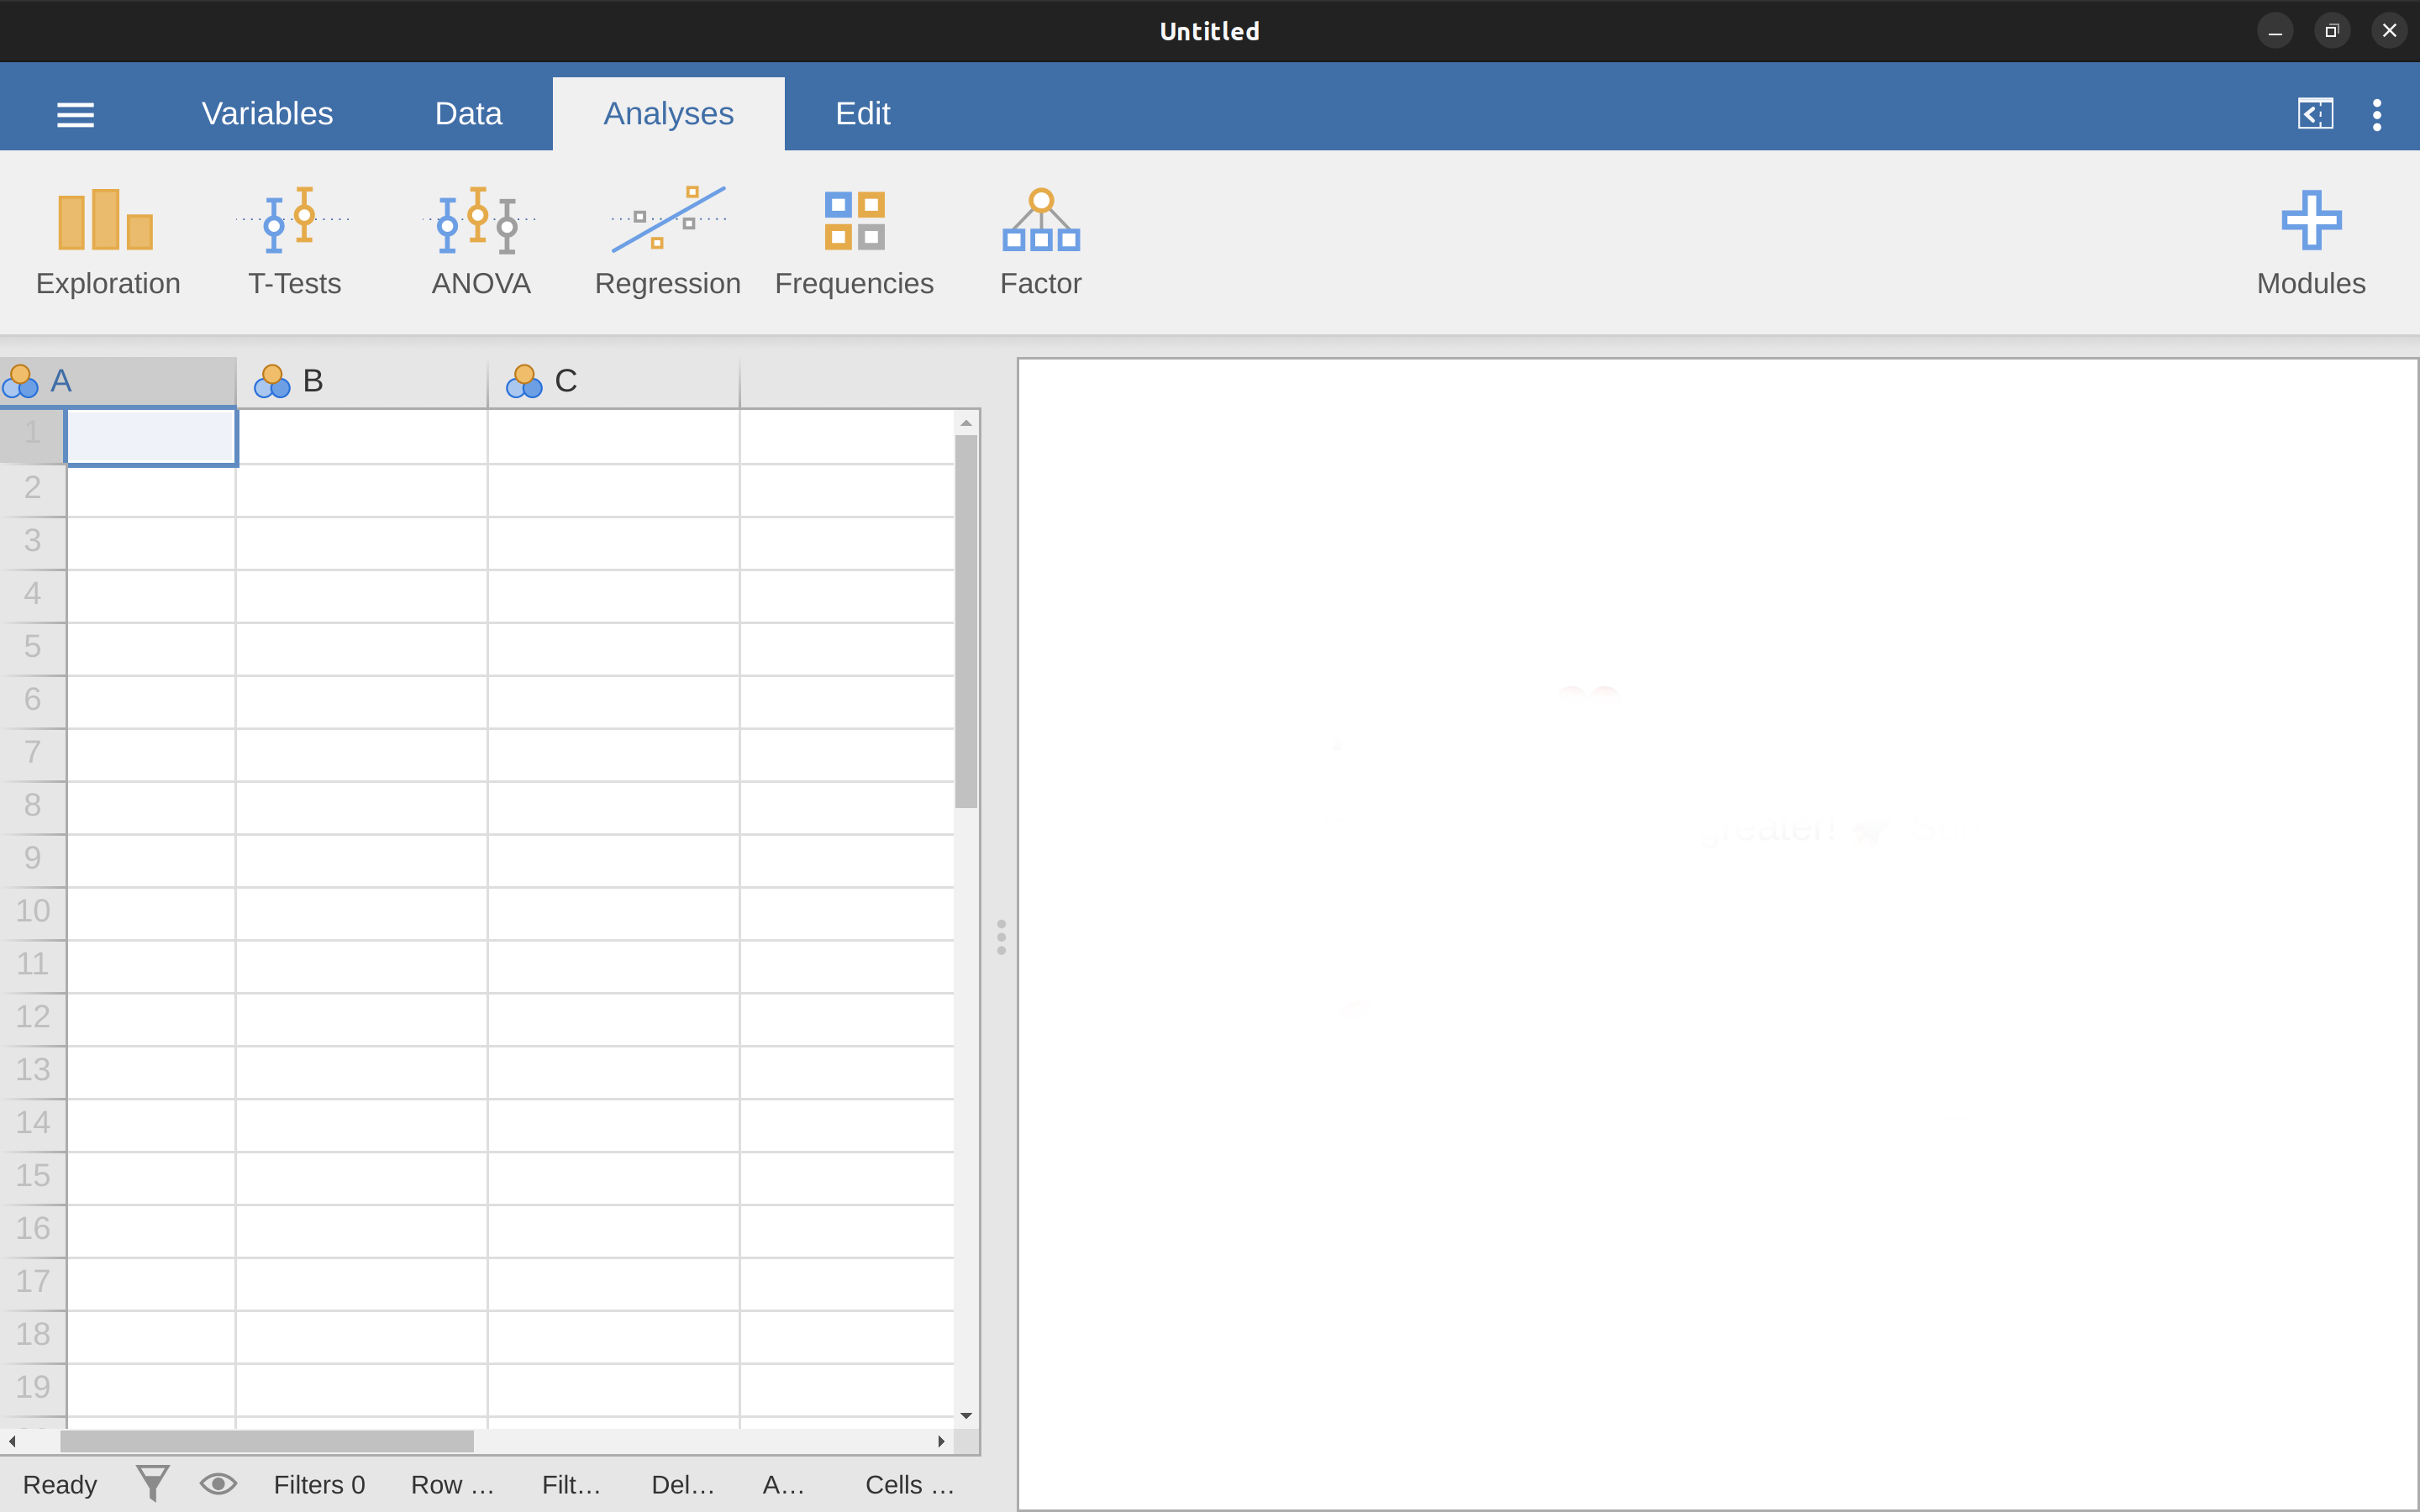
\includegraphics{./images/fig3-1.png}

}

\caption{\label{fig-fig3-1}jamovi starts up!}

\end{figure}

To the left is the spreadsheet view, and to the right is where the
results of statistical tests appear. Down the middle is a bar separating
these two regions and this can be dragged to the left or the right to
change their sizes.

It is possible to simply begin typing values into the jamovi spreadsheet
as you would in any other spreadsheet software. Alternatively, existing
data sets in the CSV (.csv) file format can be opened in jamovi.
Additionally, you can easily import SPSS, SAS, Stata and JASP files
directly into jamovi. To open a file select the File tab (three
horizontal lines signify this tab) at the top left hand corner, select
`Open' and then choose from the files listed on `Browse' depending on
whether you want to open an example or a file stored on your computer.

\hypertarget{analyses}{%
\section{Analyses}\label{analyses}}

Analyses can be selected from the analysis ribbon or menu along the top.
Selecting an analysis will present an `options panel' for that
particular analysis, allowing you to assign different variables to
different parts of the analysis, and select different options. At the
same time, the results for the analysis will appear in the right
`Results panel' and will update in real-time as you make changes to the
options.

When you have the analysis set up correctly you can dismiss the analysis
options by clicking the arrow to the top right of the optional panel. If
you wish to return to these options, you can click on the results that
were produced. In this way, you can return to any analysis that you (or
say, a colleague) created earlier.

If you decide you no longer need a particular analysis, you can remove
it with the results context menu. Right-clicking on the analysis results
will bring up a menu and by selecting `Analysis' and then `Remove' the
analysis can be removed. But more on this later. First, let's take a
more detailed look at the spreadsheet view.

\hypertarget{the-spreadsheet}{%
\section{The spreadsheet}\label{the-spreadsheet}}

In jamovi data is represented in a spreadsheet with each column
representing a `variable' and each row representing a `case' or
`participant'.

\hypertarget{variables}{%
\subsection{Variables}\label{variables}}

The most commonly used variables in jamovi are `Data Variables', these
variables simply contain data either loaded from a data file, or `typed
in' by the user. Data variables can be one of several measurement levels
(Figure~\ref{fig-fig3-2}).

\begin{figure}

{\centering 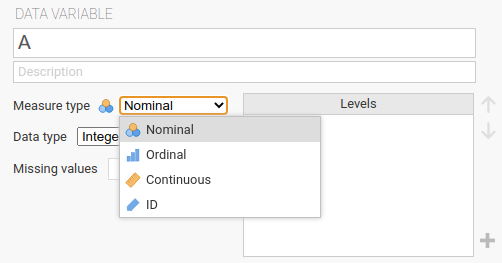
\includegraphics{./images/fig3-2.png}

}

\caption{\label{fig-fig3-2}measurement levels}

\end{figure}

These levels are designated by the symbol in the header of the
variable's column. The ID variable type is unique to jamovi. It's
intended for variables that contain identifiers that you would almost
never want to analyse. For example, a persons name, or a participant ID.
Specifying an ID variable type can improve performance when interacting
with very large data sets.

\emph{Nominal} variables are for categorical variables which are text
labels, for example a column called Gender with the values Male and
Female would be nominal. So would a person's name. Nominal variable
values can also have a numeric value. These variables are used most
often when importing data which codes values with numbers rather than
text. For example, a column in a dataset may contain the values 1 for
males, and 2 for females. It is possible to add nice `human-readable'
labels to these values with the variable editor (more on this later).

\emph{Ordinal} variables are like Nominal variables, except the values
have a specific order. An example is a Likert scale with 3 being
`strongly agree' and -3 being `strongly disagree'.

\emph{Continuous} variables are variables which exist on a continuous
scale. Examples might be height or weight. This is also referred to as
`Interval' or `Ratio scale'.

In addition, you can also specify different data types: variables have a
data type of either `Text', `Integer' or `Decimal'.

When starting with a blank spreadsheet and typing values in the variable
type will change automatically depending on the data you enter. This is
a good way to get a feel for which variable types go with which sorts of
data. Similarly, when opening a data file jamovi will try and guess the
variable type from the data in each column. In both cases this automatic
approach may not be correct, and it may be necessary to manually specify
the variable type with the variable editor.

The variable editor can be opened by selecting `Setup' from the data tab
or by double-clicking on the variable column header. The variable editor
allows you to change the name of the variable and, for data variables,
the variable type, the order of the levels, and the label displayed for
each level. Changes can be applied by clicking the `tick' to the top
right. The variable editor can be dismissed by clicking the `Hide'
arrow.

New variables can be inserted or appended to the data set using the
`add' button from the data ribbon. The `add' button also allows the
addition of computed variables.

\hypertarget{computed-variables}{%
\subsection{Computed variables}\label{computed-variables}}

Computed Variables are those which take their value by performing a
computation on other variables. Computed Variables can be used for a
range of purposes, including log transforms, z-scores, sum-scores,
negative scoring and means.

Computed variables can be added to the data set with the `add' button
available on the data tab. This will produce a formula box where you can
specify the formula. The usual arithmetic operators are available. Some
examples of formulas are:

A + B\\
LOG10(len)\\
MEAN(A, B)\\
(len - VMEAN(len)) / VSTDEV(len)

In order, these are the sum of A and B, a log (base 10) transform of
len, the mean of A and B, and the z-score of the variable
len\footnote{In later versions of jamovi there is a pre-defined function
  `Z' to compute z-scores, which is much easier!}.
Figure~\ref{fig-fig3-3} shows the jamovi screen for the new variable
computed as the z-score of len (from the `Tooth Growth' example data
set).

\begin{figure}

{\centering 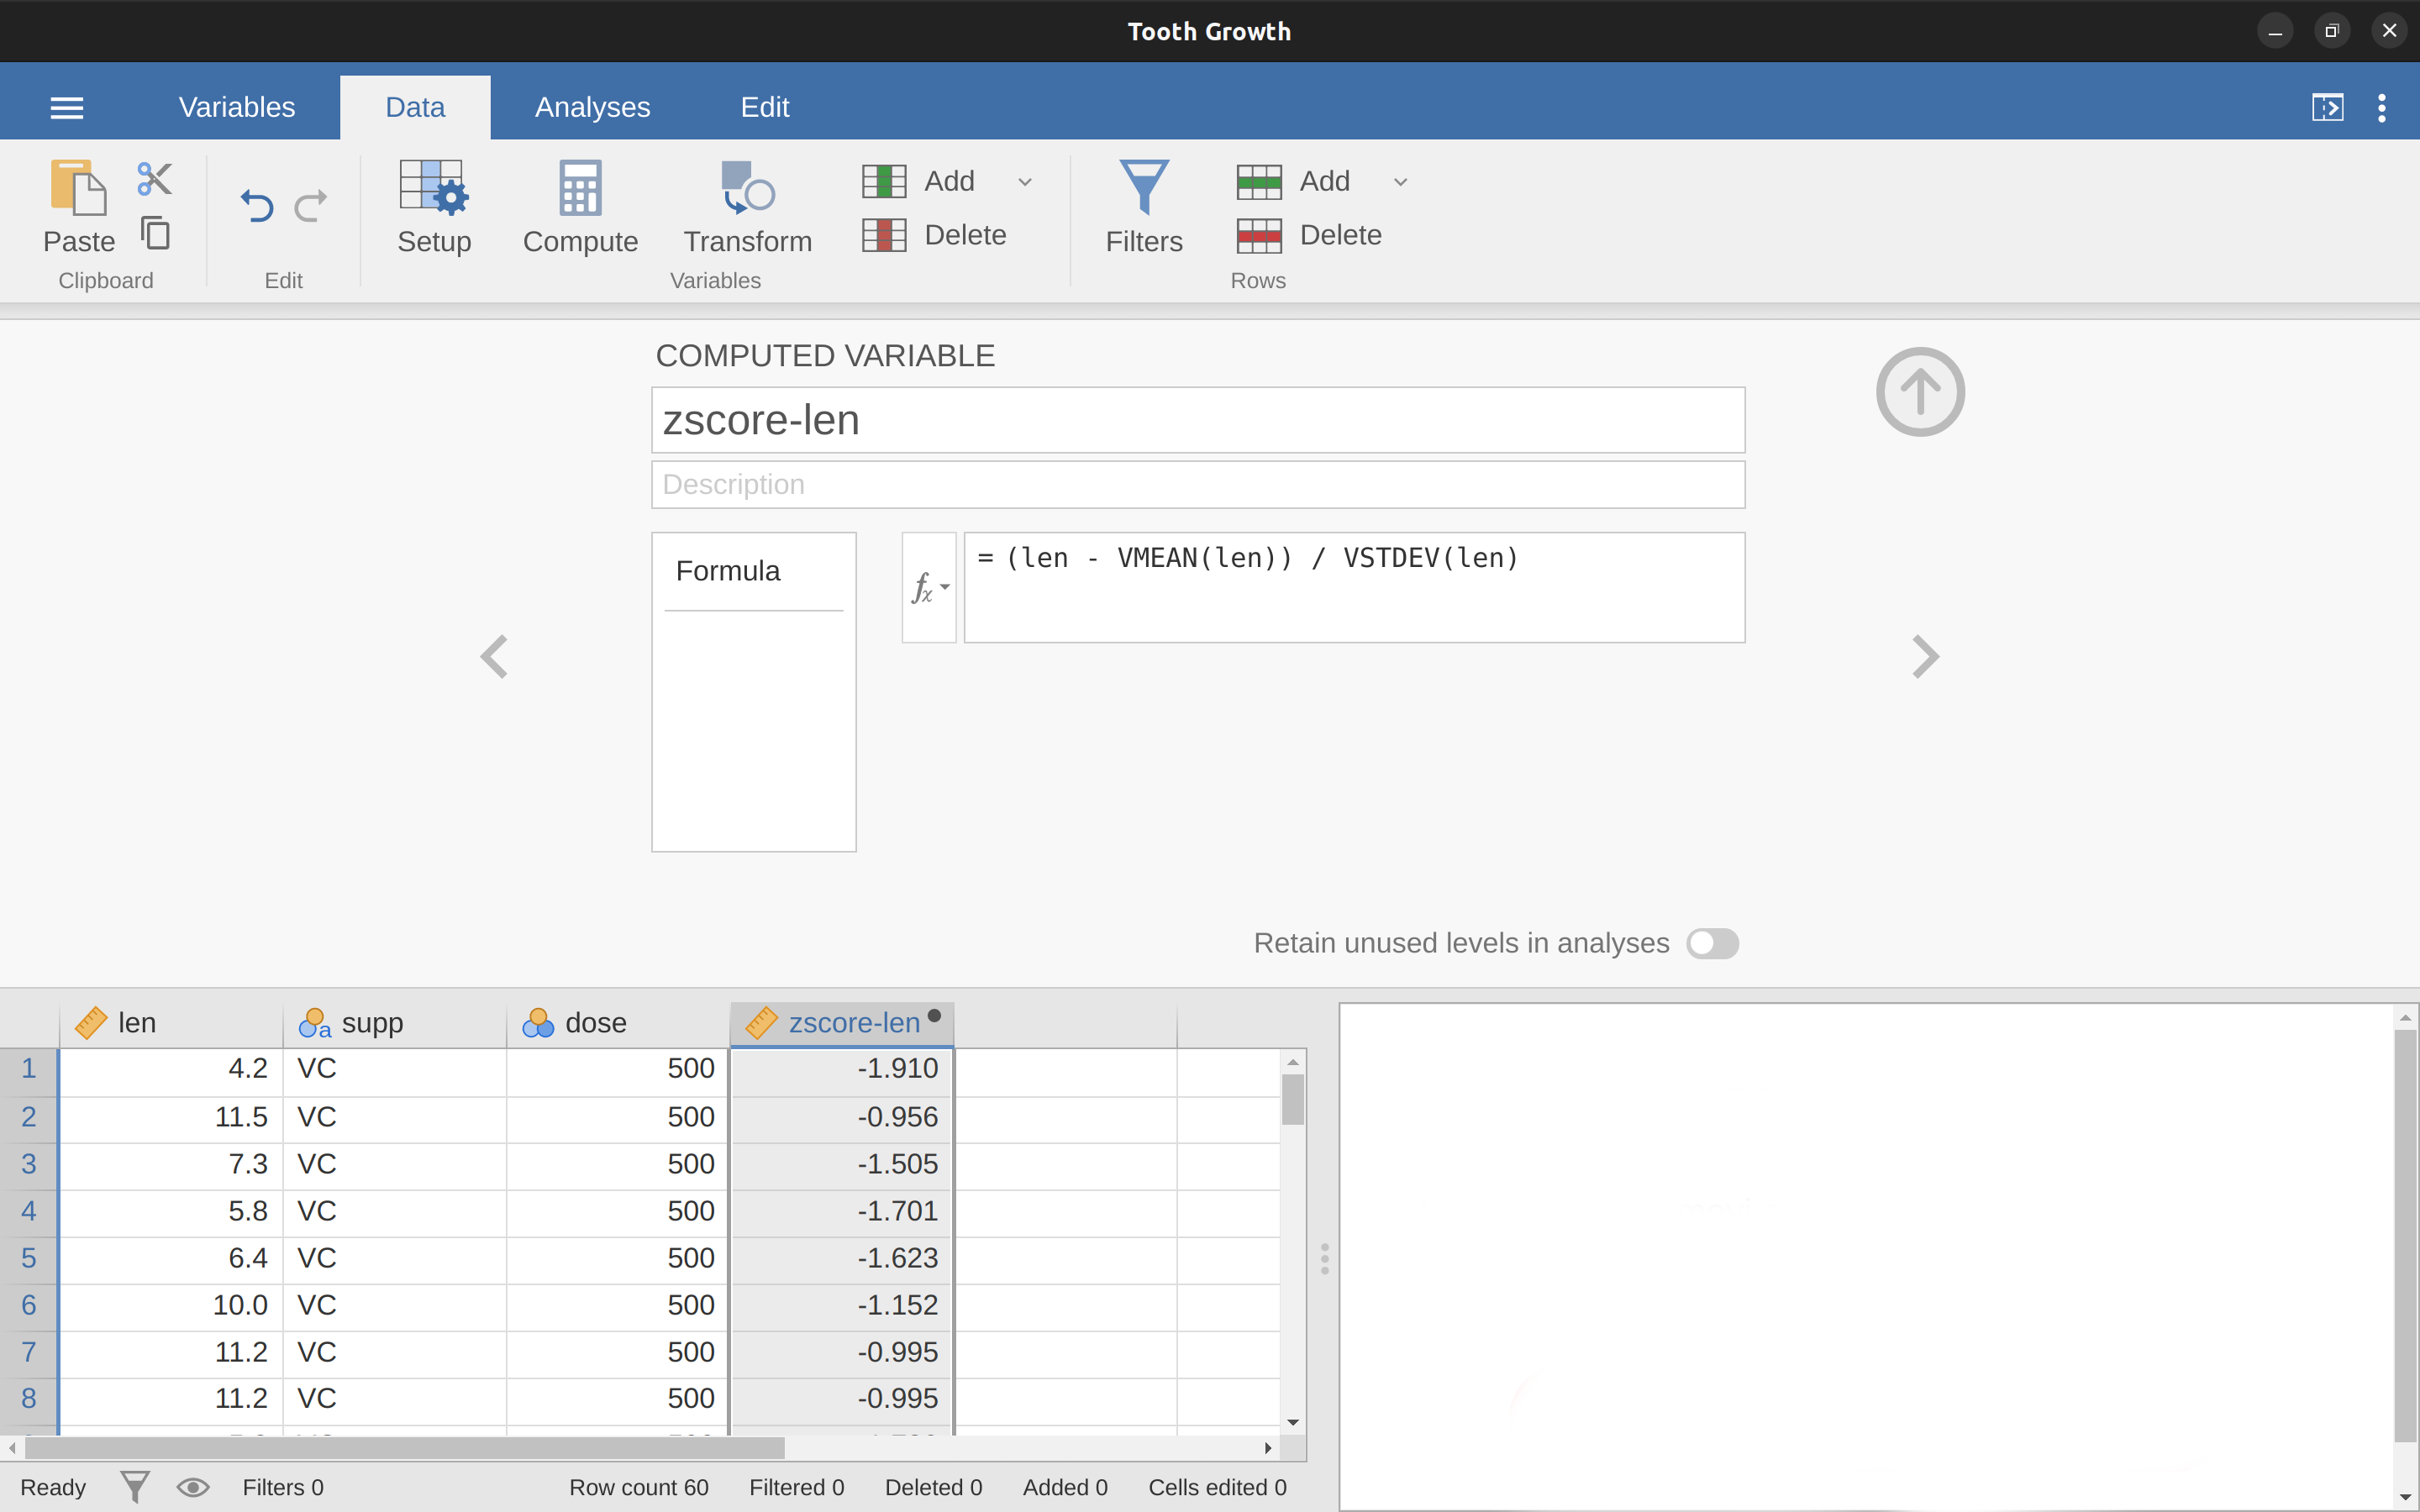
\includegraphics{./images/fig3-3.png}

}

\caption{\label{fig-fig3-3}A newly computed variable, the z-score of
`dose'}

\end{figure}

\hypertarget{v-functions}{%
\subsubsection{V-functions}\label{v-functions}}

Several functions are already available in jamovi and available from the
drop down box labelled fx. A number of functions appear in pairs, one
prefixed with a V and the other not. V functions perform their
calculation on a variable as a whole, where as non-V functions perform
their calculation row by row. For example, MEAN(A, B) will produce the
mean of A and B for each row. Where as VMEAN(A) gives the mean of all
the values in A.

\hypertarget{copy-and-paste}{%
\subsection{Copy and Paste}\label{copy-and-paste}}

jamovi produces nice American Psychological Association (APA) formatted
tables and attractive plots. It is often useful to be able to copy and
paste these, perhaps into a Word document, or into an email to a
colleague. To copy results right click on the object of interest and
from the menu select exactly what you want to copy. The menu allows you
to choose to copy only the image or the entire analysis. Selecting
``copy'' copies the content to the clipboard and this can be pasted into
other programs in the usual way. You can practice this later on when we
do some analyses.

\hypertarget{syntax-mode}{%
\subsection{Syntax mode}\label{syntax-mode}}

jamovi also provides an ``R Syntax Mode''. In this mode jamovi produces
equivalent R code for each analysis. To change to syntax mode, select
the Application menu to the top right of jamovi (a button with three
vertical dots) and click the ``Syntax mode'' checkbox there. You can
turn off syntax mode by clicking this a second time.

In syntax mode analyses continue to operate as before but now they
produce R syntax, and `ascii output' like an R session. Like all results
objects in jamovi, you can right click on these items (including the R
syntax) and copy and paste them, for example into an R session. At
present, the provided R syntax does not include the data import step and
so this must be performed manually in R. There are many resources
explaining how to import data into R and if you are interested we
recommend you take a look at these; just search on the interweb.

\hypertarget{loading-data-in-jamovi}{%
\section{Loading data in jamovi}\label{loading-data-in-jamovi}}

There are several different types of files that are likely to be
relevant to us when doing data analysis. There are two in particular
that are especially important from the perspective of this book:

\begin{itemize}
\item
  \emph{jamovi files} are those with a .omv file extension. This is the
  standard kind of file that jamovi uses to store data, and variables
  and analyses.
\item
  \emph{Comma separated value (csv) files} are those with a .csv file
  extension. These are just regular old text files and they can be
  opened with many different software programs. It's quite typical for
  people to store data in csv files, precisely because they're so
  simple.
\end{itemize}

There are also several other kinds of data file that you might want to
import into jamovi. For instance, you might want to open Microsoft Excel
spreadsheets (.xls files), or data files that have been saved in the
native file formats for other statistics software, such as SPSS or SAS.
Whichever file formats you are using, it's a good idea to create a
folder or folders especially for your jamovi data sets and analyses and
to make sure you keep these backed up regularly.

\hypertarget{importing-data-from-csv-files}{%
\subsection{Importing data from csv
files}\label{importing-data-from-csv-files}}

One quite commonly used data format is the humble ``comma separated
value'' file, also called a csv file, and usually bearing the file
extension .csv. csv files are just plain old-fashioned text files and
what they store is basically just a table of data. This is illustrated
in Figure~\ref{fig-fig3-4}, which shows a file called booksales.csv that
I've created. As you can see, each row represents the book sales data
for one month. The first row doesn't contain actual data though, it has
the names of the variables.

\begin{figure}

{\centering 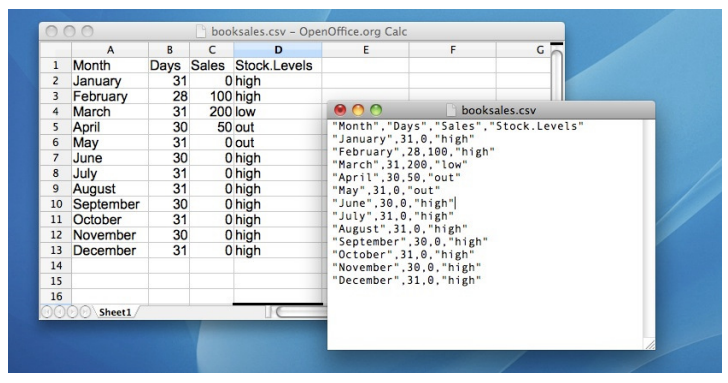
\includegraphics{./images/fig3-4.png}

}

\caption{\label{fig-fig3-4}The booksales.csv data file. On the left I
have opened the file using a spreadsheet program (OpenOffice), which
shows that the file is basically a table. On the right the same file is
open in a standard text editor (the TextEdit program on a Mac), which
shows how the file is formatted. The entries in the table are wrapped in
quote marks and separated by commas}

\end{figure}

It's easy to open csv files in jamovi. From the top left menu (the
button with three parallel lines) choose `Open' and browse to where you
have stored the csv file on your computer. If you're on a Mac, it'll
look like the usual Finder window that you use to choose a file; on
Windows it looks like an Explorer window. An example of what it looks
like on a Mac is shown in Figure~\ref{fig-fig3-5}. I'm assuming that
you're familiar with your own computer, so you should have no problem
finding the csv file that you want to import! Find the one you want,
then click on the ``Open'' button.

\begin{figure}

{\centering 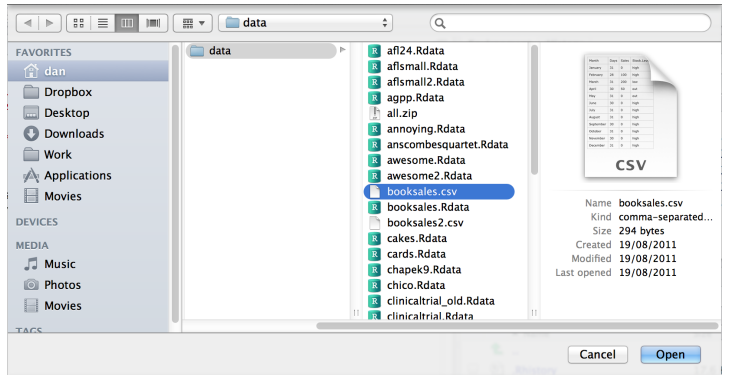
\includegraphics{./images/fig3-5.png}

}

\caption{\label{fig-fig3-5}A dialog box on a Mac asking you to select
the csv file jamovi should try to import. Mac users will recognise this
immediately, it's the usual way in which a Mac asks you to find a file.
Windows users won't see this, instead they'll see the usual explorer
window that Windows always gives you when it wants you to select a file}

\end{figure}

There are a few things that you can check to make sure that the data
gets imported correctly:

\begin{itemize}
\tightlist
\item
  Heading. Does the first row of the file contain the names for each
  variable - a `header' row? The booksales.csv file has a header, so
  that's a yes.
\item
  Decimal. What character is used to specify the decimal point? In
  English speaking countries this is almost always a period (i.e., .).
  That's not universally true though, many European countries use a
  comma.
\item
  Quote. What character is used to denote a block of text? That's
  usually going to be a double quote mark (``). It is for the
  booksales.csv file.
\end{itemize}

\hypertarget{importing-unusual-data-files}{%
\section{Importing unusual data
files}\label{importing-unusual-data-files}}

Throughout this book I've assumed that your data are stored as a jamovi
.omv file or as a ``properly'' formatted csv file. However, in real life
that's not a terribly plausible assumption to make so I'd better talk
about some of the other possibilities that you might run into.

\hypertarget{loading-data-from-text-files}{%
\subsection{Loading data from text
files}\label{loading-data-from-text-files}}

The first thing I should point out is that if your data are saved as a
text file but aren't quite in the proper csv format then there's still a
pretty good chance that jamovi will be able to open it. You just need to
try it and see if it works. Sometimes though you will need to change
some of the formatting. The ones that I've often found myself needing to
change are:

\begin{itemize}
\tightlist
\item
  header. A lot of the time when you're storing data as a csv file the
  first row actually contains the column names and not data. If that's
  not true then it's a good idea to open up the csv file in a
  spreadsheet programme such as Open Office and add the header row
  manually.
\item
  sep. As the name ``comma separated value'' indicates, the values in a
  row of a csv file are usually separated by commas. This isn't
  universal, however. In Europe the decimal point is typically written
  as , instead of . and as a consequence it would be somewhat awkward to
  use , as the separator. Therefore it is not unusual to use ; instead
  of , as the separator. At other times, I've seen a TAB character used.
\item
  quote. It's conventional in csv files to include a quoting character
  for textual data. As you can see by looking at the booksales.csv file,
  this is usually a double quote character, ``. But sometimes there is
  no quoting character at all, or you might see a single quote mark '
  used instead.
\item
  skip. It's actually very common to receive CSV files in which the
  first few rows have nothing to do with the actual data. Instead, they
  provide a human readable summary of where the data came from, or maybe
  they include some technical info that doesn't relate to the data.
\item
  missing values. Often you'll get given data with missing values. For
  one reason or another, some entries in the table are missing. The data
  file needs to include a ``special'' value to indicate that the entry
  is missing. By default jamovi assumes that this value is
  99\footnote{You can change the default value for missing values in
    jamovi from the top right menu (three vertical dots), but this only
    works at the time of importing data files into jamovi. The default
    missing value in the dataset should not be a valid number associated
    with any of the variables, e.g.~you could use -9999 as this is
    unlikely to be a valid value.}, for both numeric and text data, so
  you should make sure that, where necessary, all missing values in the
  csv file are replaced with 99 (or -9999; whichever you choose) before
  opening / importing the file into jamovi. Once you have opened /
  imported the file into jamovi all the missing values are converted to
  blank or greyed out cells in the jamovi spreadsheet view. You can also
  change the missing value for each variable as an option in the Data -
  Setup view.
\end{itemize}

\hypertarget{loading-data-from-spss-and-other-statistics-packages}{%
\subsection{Loading data from SPSS (and other statistics
packages)}\label{loading-data-from-spss-and-other-statistics-packages}}

The commands listed above are the main ones we'll need for data files in
this book. But in real life we have many more possibilities. For
example, you might want to read data files in from other statistics
programs. Since SPSS is probably the most widely used statistics package
in psychology, it's worth mentioning that jamovi can also import SPSS
data files (file extension .sav). Just follow the instructions above for
how to open a csv file, but this time navigate to the .sav file you want
to import. For SPSS files, jamovi will regard all values as missing if
they are regarded as ``system missing'' files in SPSS. The `Default
missings' value does not seem to work as expected when importing SPSS
files, so be aware of this - you might need another step: import the
SPSS file into jamovi, then export as a csv file before re-opening in
jamovi.\footnote{I know this is a bit of a fudge, but it does work and
  hopefully this will be fixed in a later version of jamovi.}

And that's pretty much it, at least as far as SPSS goes. As far as other
statistical software goes, jamovi can also directly open / import SAS
and STATA files.

\hypertarget{loading-excel-files}{%
\subsection{Loading Excel files}\label{loading-excel-files}}

A different problem is posed by Excel files. Despite years of yelling at
people for sending data to me encoded in a proprietary data format, I
get sent a lot of Excel files. The way to handle Excel files is to open
them up first in Excel or another spreadsheet programme that can handle
Excel files, and then export the data as a csv file before opening /
importing the csv file into jamovi.

\hypertarget{sec-Changing-data-from-one-level-to-another}{%
\section{Changing data from one level to
another}\label{sec-Changing-data-from-one-level-to-another}}

Sometimes you want to change the variable level. This can happen for all
sorts of reasons. Sometimes when you import data from files, it can come
to you in the wrong format. Numbers sometimes get imported as nominal,
text values. Dates may get imported as text. ParticipantID values can
sometimes be read as continuous: nominal values can sometimes be read as
ordinal or even continuous. There's a good chance that sometimes you'll
want to convert a variable from one measurement level into another one.
Or, to use the correct term, you want to \textbf{coerce} the variable
from one class into another.

Earlier we saw how to specify different variable levels, and if you want
to change a variable's measurement level then you can do this in the
jamovi data view for that variable. Just click the check box for the
measurement level you want - continuous, ordinal, or nominal.

\hypertarget{installing-add-on-modules-into-jamovi}{%
\section{Installing add-on modules into
jamovi}\label{installing-add-on-modules-into-jamovi}}

A really great feature of jamovi is the ability to install add-on
modules from the jamovi library. These add-on modules have been
developed by the jamovi community, i.e., jamovi users and developers who
have created special software add-ons that do other, usually more
advanced, analyses that go beyond the capabilities of the base jamovi
program.

To install add-on modules, just click on the large \(+\) in the top
right of the jamovi window, select ``jamovi-library'' and then browse
through the various add-on modules that are available. Choose the one(s)
you want, and then install them, as in Figure~\ref{fig-fig3-6}. It's
that easy. The newly installed modules can then be accessed from the
``Analyses'' button bar. Try it\ldots useful add-on modules to install
include ``scatr'' (added under ``Descriptives'') and \(R_j\).

\begin{figure}

{\centering 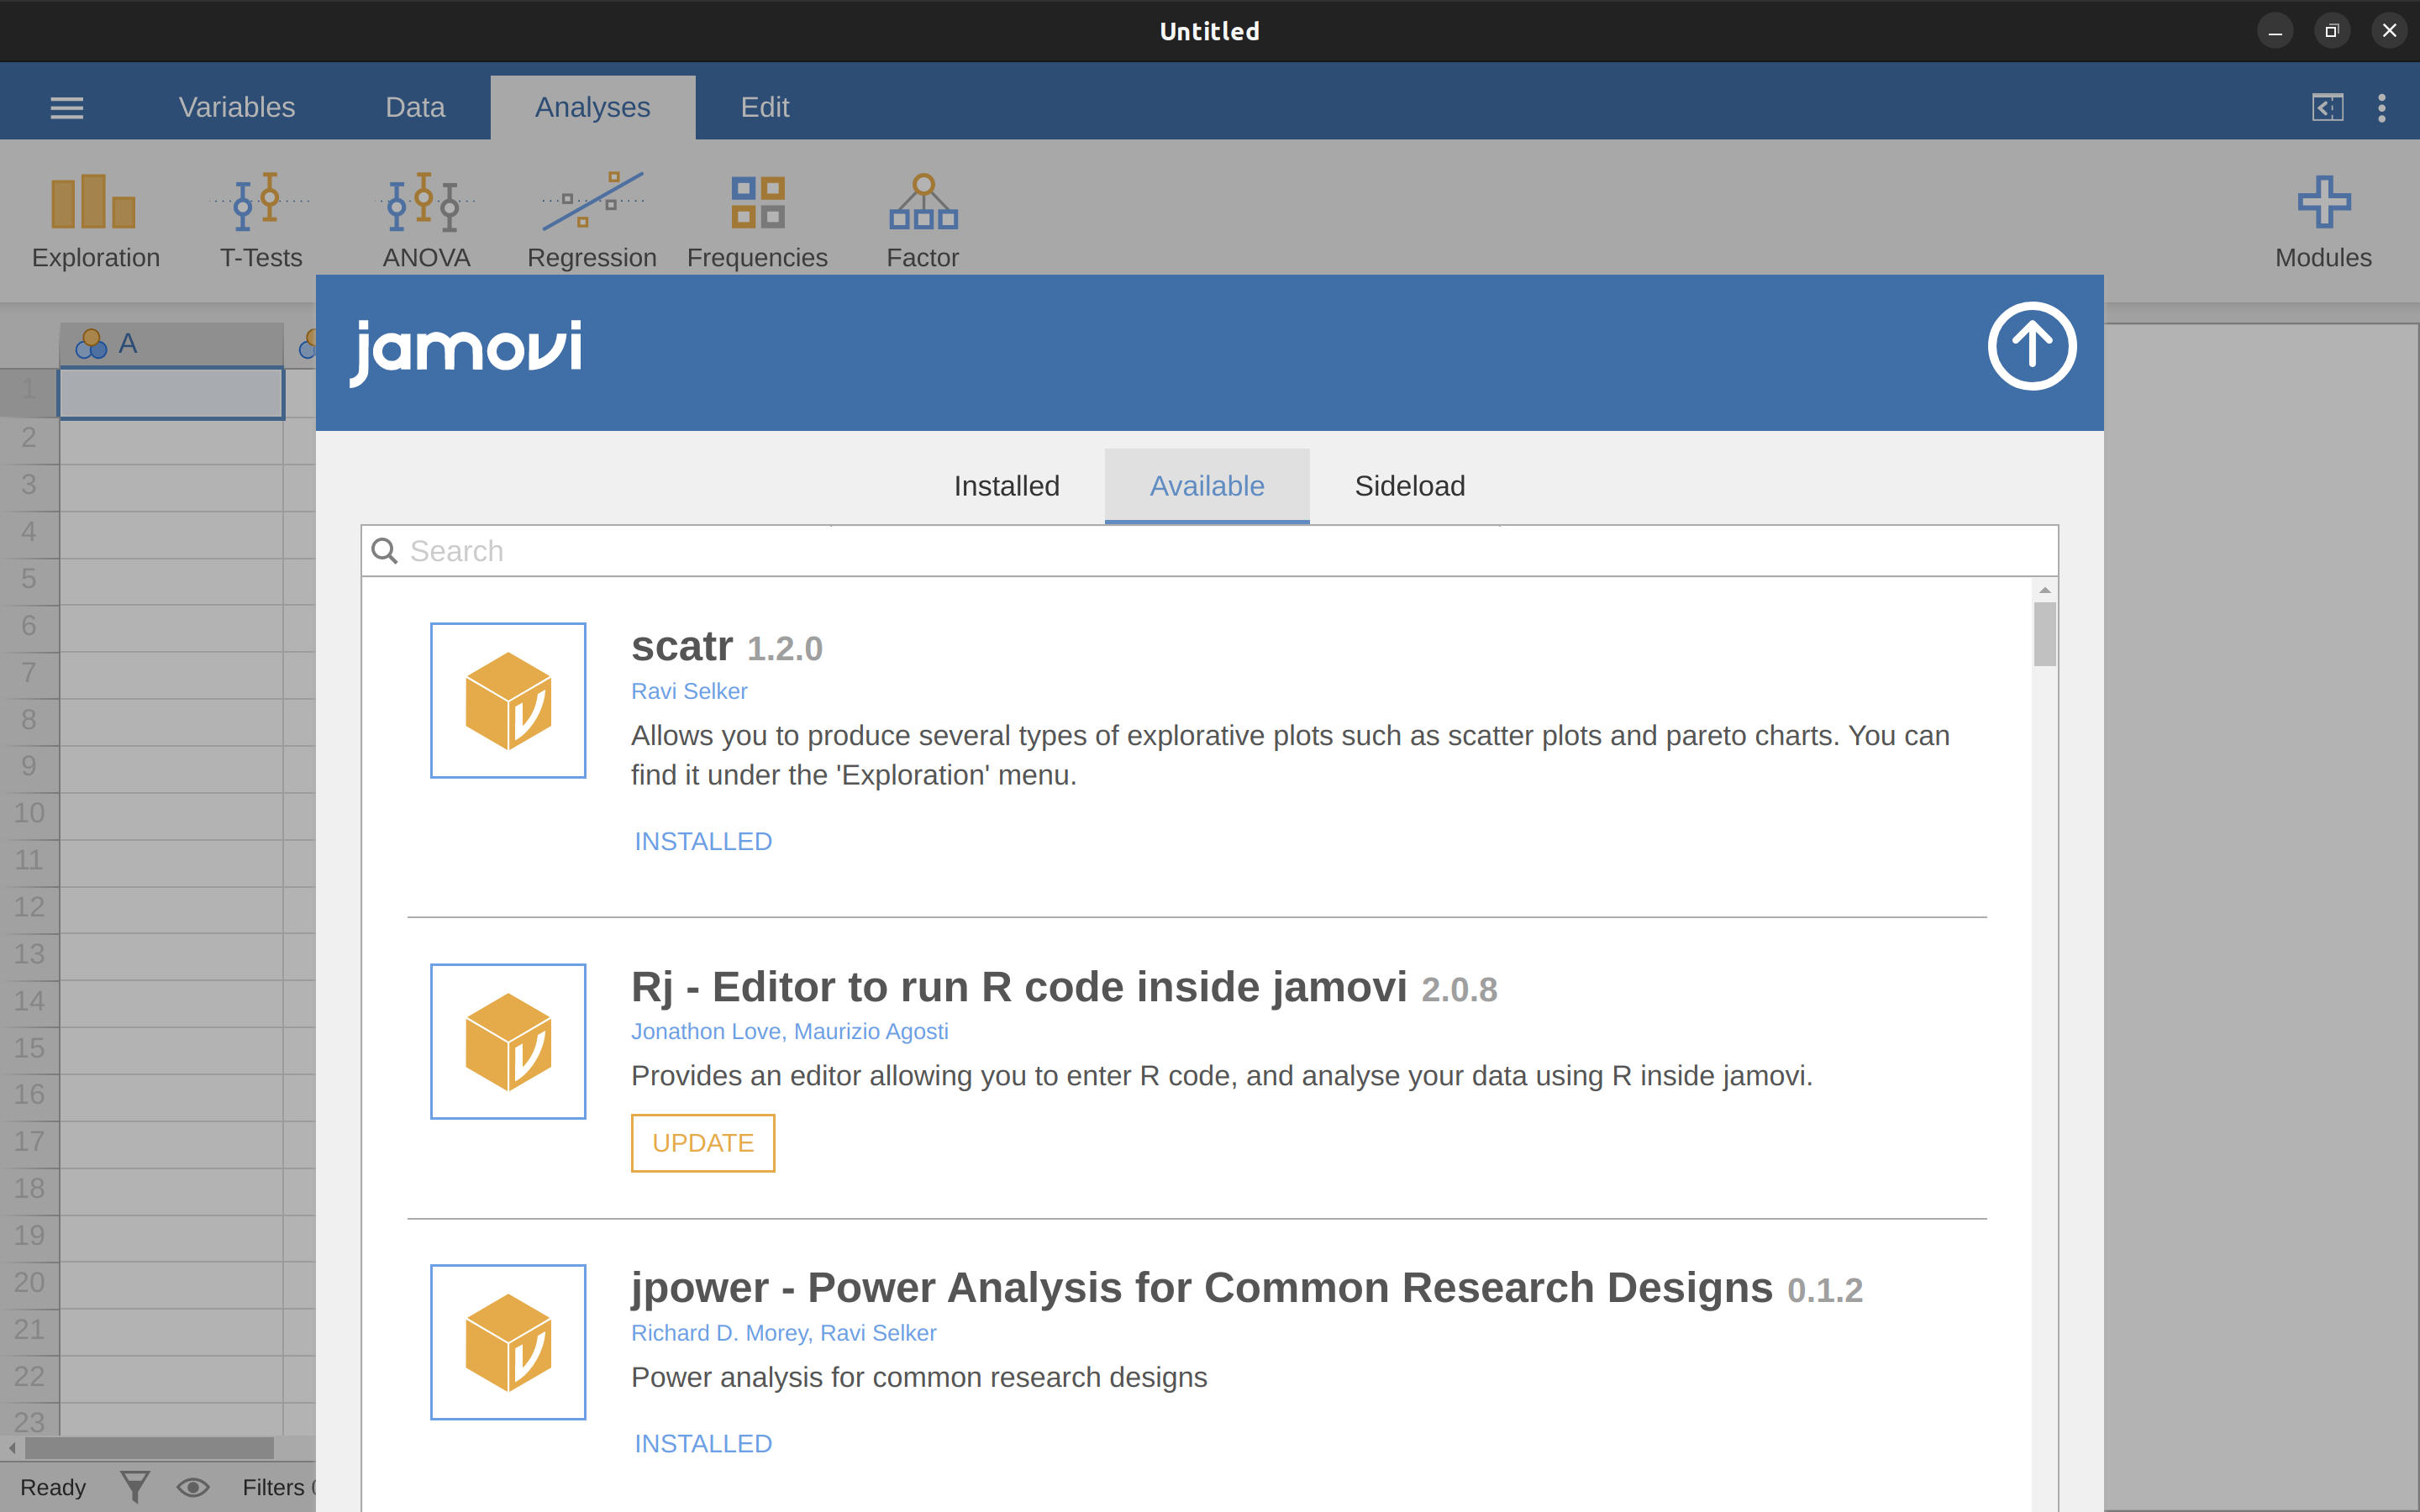
\includegraphics{./images/fig3-6.png}

}

\caption{\label{fig-fig3-6}Installing add-on modules in jamovi}

\end{figure}

\hypertarget{quitting-jamovi}{%
\section{Quitting jamovi}\label{quitting-jamovi}}

There's one last thing I should cover in this chapter: how to quit
jamovi. It's not hard, just close the program the same way you would any
other program. However, what you might want to do before you quit is
save your work! There are two parts to this: saving any changes to the
data set, and saving the analyses that you ran.

It is good practice to save any changes to the data set as a \emph{new}
data set. That way you can always go back to the original data. To save
any changes in jamovi, select `Export'\ldots{}`Data' from the main
jamovi menu (button with three horizontal bars in the top left) and
create a new file name for the changed data set.

Alternatively, you can save \emph{both} the changed data and any
analyses you have undertaken by saving as a jamovi file. To do this,
from the main jamovi menu select `Save as' and type in a file name for
this `jamovi file (.omv)'. Remember to save the file in a location where
you can find it again later. I usually create a new folder for specific
data sets and analyses.

\hypertarget{summary-1}{%
\section{Summary}\label{summary-1}}

Every book that tries to teach a new statistical software program to
novices has to cover roughly the same topics, and in roughly the same
order. Ours is no exception, and so in the grand tradition of doing it
just the same way everyone else did it, this chapter covered the
following topics:

\begin{itemize}
\tightlist
\item
  \protect\hyperlink{installing-jamovi}{Installing jamovi}. We
  downloaded and installed jamovi, and started it up.
\item
  \protect\hyperlink{analyses}{Analyses}. We very briefly oriented to
  the part of jamovi where analyses are done and results appear, but
  then deferred this until later in the book.
\item
  \protect\hyperlink{the-spreadsheet}{The spreadsheet}. We spent more
  time looking at the spreadsheet part of jamovi, and considered
  different variable types, and how to compute new variables.
\item
  \protect\hyperlink{loading-data-in-jamovi}{Loading data in jamovi}. We
  also saw how to load data files in jamovi.
\item
  \protect\hyperlink{importing-unusual-data-files}{Importing unusual
  data files}. Then we figured out how to open other data files, from
  different file types.
\item
  \protect\hyperlink{sec-Changing-data-from-one-level-to-another}{Changing
  data from one level to another}. And saw that sometimes we need to
  coerce data from one type to another.
\item
  \protect\hyperlink{installing-add-on-modules-into-jamovi}{Installing
  add-on modules into jamovi}. Installing add-on modules from the jamovi
  community really extends jamovi capabilities.
\item
  \protect\hyperlink{quitting-jamovi}{Quitting jamovi}. Finally, we
  looked at good practice in terms of saving your data set and analyses
  when you have finished and are about to quit jamovi.
\end{itemize}

We still haven't arrived at anything that resembles data analysis. Maybe
the next Chapter will get us a bit closer!

\begin{center}\rule{0.5\linewidth}{0.5pt}\end{center}

\part{Working with data}

\hypertarget{sec-Descriptive-statistics}{%
\chapter{Descriptive statistics}\label{sec-Descriptive-statistics}}

Any time that you get a new data set to look at one of the first tasks
that you have to do is find ways of summarising the data in a compact,
easily understood fashion. This is what \textbf{descriptive statistics}
(as opposed to inferential statistics) is all about. In fact, to many
people the term ``statistics'' is synonymous with descriptive
statistics. It is this topic that we'll consider in this chapter, but
before going into any details, let's take a moment to get a sense of why
we need descriptive statistics. To do this, let's open the
aflsmall\_margins file and see what variables are stored in the file,
see Figure~\ref{fig-fig4-1}.

\begin{figure}

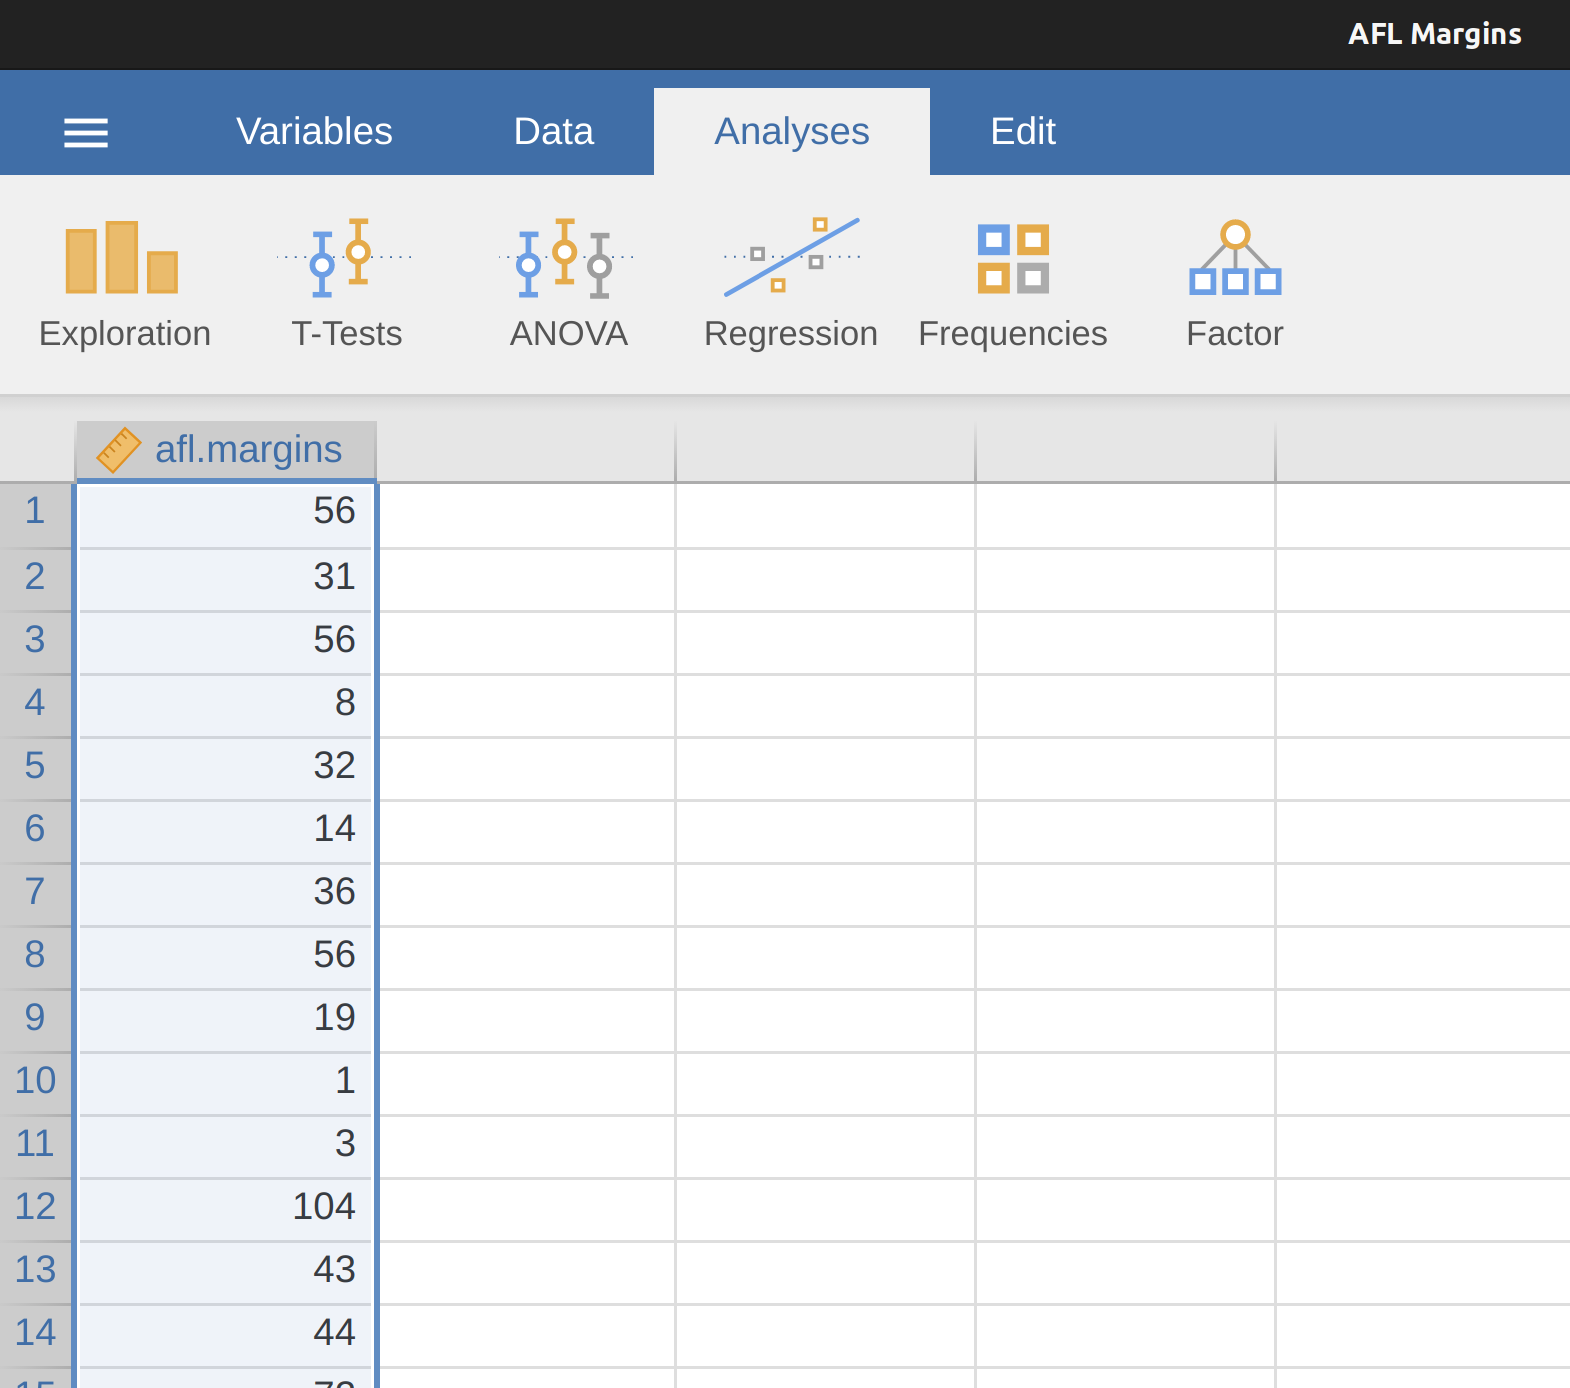
\includegraphics{./images/fig4-1.png} \hfill{}

\caption{\label{fig-fig4-1}A screenshot of jamovi showing the variables
stored in the aflsmallmargins.csv file}

\end{figure}

In fact, there is just one variable here, afl.margins. We'll focus a bit
on this variable in this chapter, so I'd better tell you what it is.
Unlike most of the data sets in this book, this is actually real data,
relating to the Australian Football League (AFL).\footnote{Note for
  non-Australians: the AFL is an Australian rules football competition.
  You don't need to know anything about Australian rules in order to
  follow this section.} The afl.margins variable contains the winning
margin (number of points) for all 176 home and away games played during
the 2010 season.

This output doesn't make it easy to get a sense of what the data are
actually saying. Just ``looking at the data'' isn't a terribly effective
way of understanding data. In order to get some idea about what the data
are actually saying we need to calculate some descriptive statistics
(this chapter) and draw some nice pictures
(Chapter~\ref{sec-Drawing-graphs}). Since the descriptive statistics are
the easier of the two topics I'll start with those, but nevertheless
I'll show you a histogram of the afl.margins data since it should help
you get a sense of what the data we're trying to describe actually look
like, see Figure~\ref{fig-fig4-2}. We'll talk a lot more about how to
draw histograms in Section~\ref{sec-Histograms} in the next chapter. For
now, it's enough to look at the histogram and note that it provides a
fairly interpretable representation of the afl.margins data.

\begin{figure}

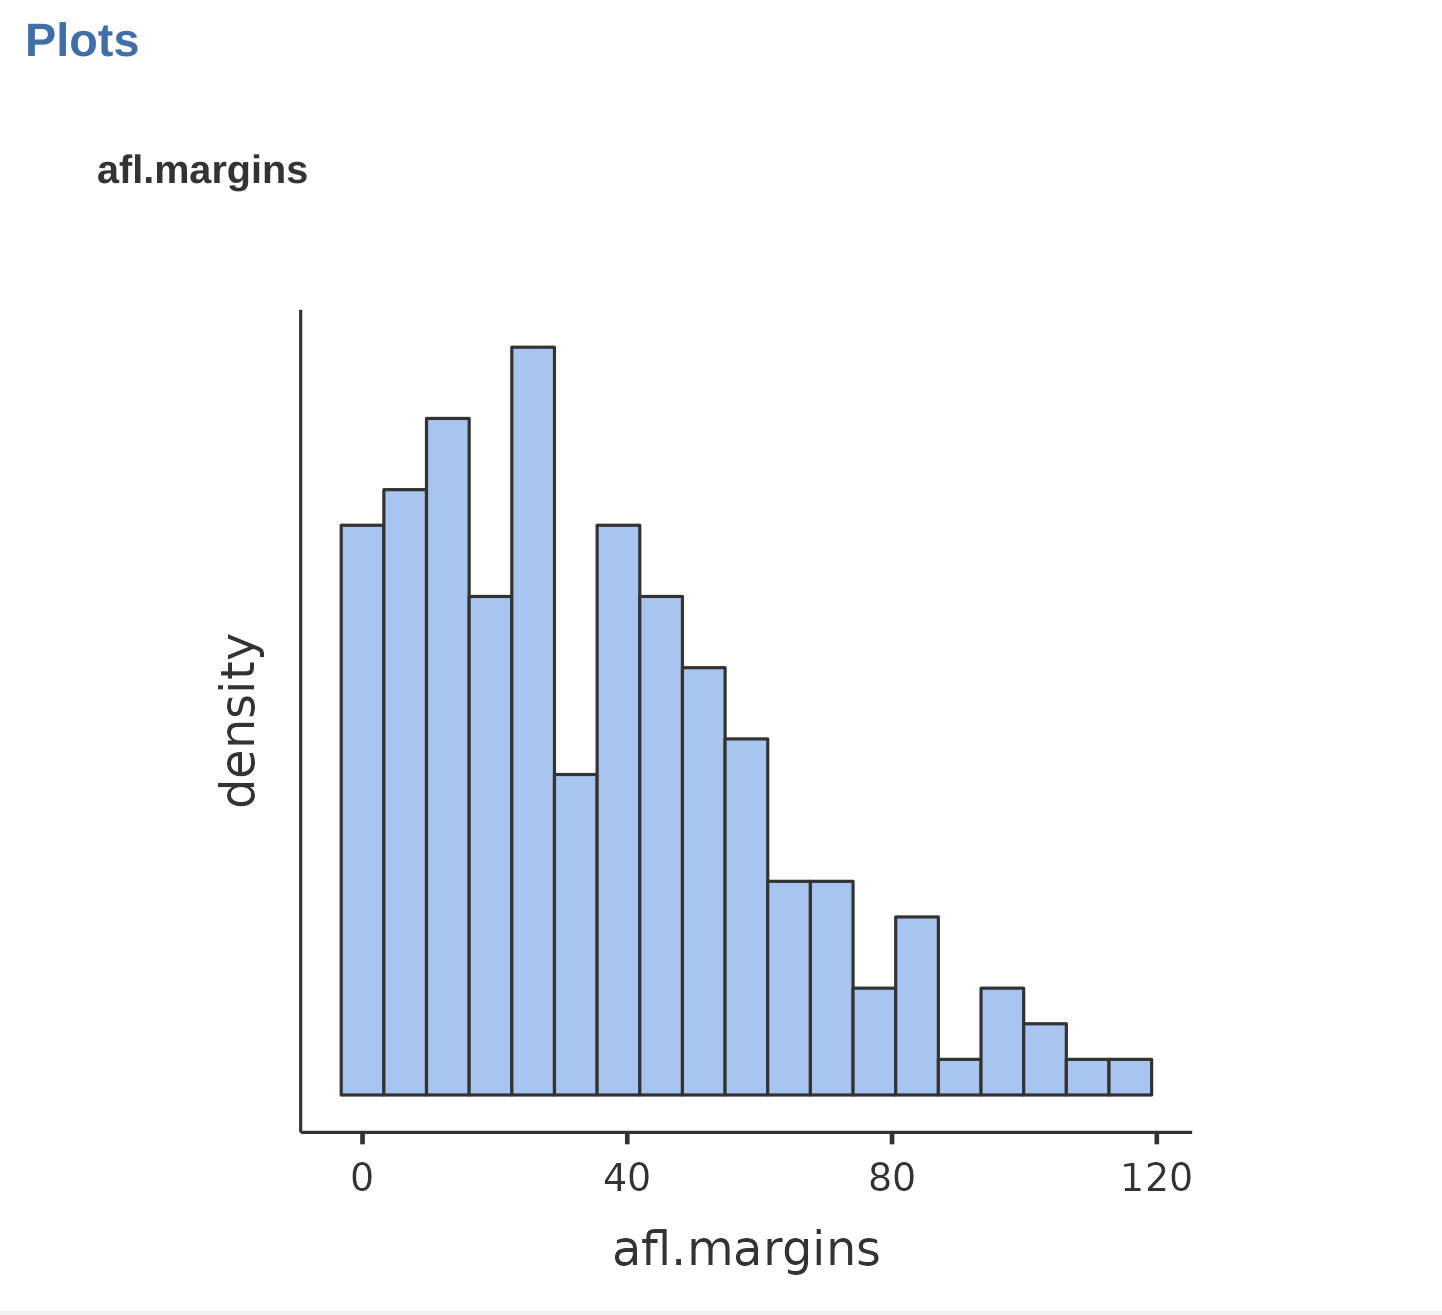
\includegraphics{./images/fig4-2.png} \hfill{}

\caption{\label{fig-fig4-2}A histogram of the AFL 2010 winning margin
data (the afl.margins variable). As you might expect, the larger the
winning margin the less frequently you tend to see it}

\end{figure}

\hypertarget{measures-of-central-tendency}{%
\section{Measures of central
tendency}\label{measures-of-central-tendency}}

Drawing pictures of the data, as I did in Figure~\ref{fig-fig4-2}, is an
excellent way to convey the ``gist'' of what the data is trying to tell
you. It's often extremely useful to try to condense the data into a few
simple ``summary'' statistics. In most situations, the first thing that
you'll want to calculate is a measure of \textbf{central tendency}. That
is, you'd like to know something about where the ``average'' or
``middle'' of your data lies. The three most commonly used measures are
the mean, median and mode. I'll explain each of these in turn, and then
discuss when each of them is useful.

\hypertarget{the-mean}{%
\subsection{The mean}\label{the-mean}}

The \textbf{mean} of a set of observations is just a normal,
old-fashioned average. Add all of the values up, and then divide by the
total number of values. The first five AFL winning margins were 56, 31,
56, 8 and 32, so the mean of these observations is just:

\[
\frac{56 + 31 + 56 + 8 + 32}{5} = \frac{183}{5} = 36.60
\] Of course, this definition of the mean isn't news to anyone. Averages
(i.e., means) are used so often in everyday life that this is pretty
familiar stuff. However, since the concept of a mean is something that
everyone already understands, I'll use this as an excuse to start
introducing some of the mathematical notation that statisticians use to
describe this calculation, and talk about how the calculations would be
done in jamovi.

The first piece of notation to introduce is \(N\), which we'll use to
refer to the number of observations that we're averaging (in this case
\(N = 5\)). Next, we need to attach a label to the observations
themselves. It's traditional to use X for this, and to use subscripts to
indicate which observation we're actually talking about. That is, we'll
use \(X_1\) to refer to the first observation, \(X_2\) to refer to the
second observation, and so on all the way up to \(X_N\) for the last
one. Or, to say the same thing in a slightly more abstract way, we use
\(X_i\) to refer to the i-th observation. Just to make sure we're clear
on the notation, Table~\ref{tbl-tab4-1} lists the 5 observations in the
afl.margins variable, along with the mathematical symbol used to refer
to it and the actual value that the observation corresponds to.

\hypertarget{tbl-tab4-1}{}
 
  \providecommand{\huxb}[2]{\arrayrulecolor[RGB]{#1}\global\arrayrulewidth=#2pt}
  \providecommand{\huxvb}[2]{\color[RGB]{#1}\vrule width #2pt}
  \providecommand{\huxtpad}[1]{\rule{0pt}{#1}}
  \providecommand{\huxbpad}[1]{\rule[-#1]{0pt}{#1}}

\begin{table}[ht]
\caption{\label{tbl-tab4-1}Observations in the afl.margins variable }\tabularnewline

\begin{centerbox}
\begin{threeparttable}
\setlength{\tabcolsep}{0pt}
\begin{tabularx}{0.9\textwidth}{p{0.3\textwidth} p{0.3\textwidth} p{0.3\textwidth}}


\hhline{>{\huxb{0, 0, 0}{0.4}}->{\huxb{0, 0, 0}{0.4}}->{\huxb{0, 0, 0}{0.4}}-}
\arrayrulecolor{black}

\multicolumn{1}{!{\huxvb{0, 0, 0}{0}}p{0.3\textwidth}!{\huxvb{0, 0, 0}{0}}}{\cellcolor[RGB]{242, 242, 242}\hspace{0pt}\parbox[b]{0.3\textwidth-0pt-6pt}{\huxtpad{6pt + 1em}\centering \textbf{the observation}\huxbpad{6pt}}} &
\multicolumn{1}{p{0.3\textwidth}!{\huxvb{0, 0, 0}{0}}}{\cellcolor[RGB]{242, 242, 242}\hspace{6pt}\parbox[b]{0.3\textwidth-6pt-6pt}{\huxtpad{6pt + 1em}\centering \textbf{its symbol}\huxbpad{6pt}}} &
\multicolumn{1}{p{0.3\textwidth}!{\huxvb{0, 0, 0}{0}}}{\cellcolor[RGB]{242, 242, 242}\hspace{6pt}\parbox[b]{0.3\textwidth-6pt-0pt}{\huxtpad{6pt + 1em}\centering \textbf{the observed value}\huxbpad{6pt}}} \tabularnewline[-0.5pt]


\hhline{>{\huxb{0, 0, 0}{0.4}}->{\huxb{0, 0, 0}{0.4}}->{\huxb{0, 0, 0}{0.4}}-}
\arrayrulecolor{black}

\multicolumn{1}{!{\huxvb{0, 0, 0}{0}}p{0.3\textwidth}!{\huxvb{0, 0, 0}{0}}}{\hspace{0pt}\parbox[b]{0.3\textwidth-0pt-6pt}{\huxtpad{6pt + 1em}\centering winning margin, game 1\huxbpad{6pt}}} &
\multicolumn{1}{p{0.3\textwidth}!{\huxvb{0, 0, 0}{0}}}{\hspace{6pt}\parbox[b]{0.3\textwidth-6pt-6pt}{\huxtpad{6pt + 1em}\centering \( X_1 \)\huxbpad{6pt}}} &
\multicolumn{1}{p{0.3\textwidth}!{\huxvb{0, 0, 0}{0}}}{\hspace{6pt}\parbox[b]{0.3\textwidth-6pt-0pt}{\huxtpad{6pt + 1em}\centering 56 points\huxbpad{6pt}}} \tabularnewline[-0.5pt]


\hhline{}
\arrayrulecolor{black}

\multicolumn{1}{!{\huxvb{0, 0, 0}{0}}p{0.3\textwidth}!{\huxvb{0, 0, 0}{0}}}{\cellcolor[RGB]{242, 242, 242}\hspace{0pt}\parbox[b]{0.3\textwidth-0pt-6pt}{\huxtpad{6pt + 1em}\centering winning margin, game 2\huxbpad{6pt}}} &
\multicolumn{1}{p{0.3\textwidth}!{\huxvb{0, 0, 0}{0}}}{\cellcolor[RGB]{242, 242, 242}\hspace{6pt}\parbox[b]{0.3\textwidth-6pt-6pt}{\huxtpad{6pt + 1em}\centering \( X_2 \)\huxbpad{6pt}}} &
\multicolumn{1}{p{0.3\textwidth}!{\huxvb{0, 0, 0}{0}}}{\cellcolor[RGB]{242, 242, 242}\hspace{6pt}\parbox[b]{0.3\textwidth-6pt-0pt}{\huxtpad{6pt + 1em}\centering 31 points\huxbpad{6pt}}} \tabularnewline[-0.5pt]


\hhline{}
\arrayrulecolor{black}

\multicolumn{1}{!{\huxvb{0, 0, 0}{0}}p{0.3\textwidth}!{\huxvb{0, 0, 0}{0}}}{\hspace{0pt}\parbox[b]{0.3\textwidth-0pt-6pt}{\huxtpad{6pt + 1em}\centering winning margin, game 3\huxbpad{6pt}}} &
\multicolumn{1}{p{0.3\textwidth}!{\huxvb{0, 0, 0}{0}}}{\hspace{6pt}\parbox[b]{0.3\textwidth-6pt-6pt}{\huxtpad{6pt + 1em}\centering \( X_3 \)\huxbpad{6pt}}} &
\multicolumn{1}{p{0.3\textwidth}!{\huxvb{0, 0, 0}{0}}}{\hspace{6pt}\parbox[b]{0.3\textwidth-6pt-0pt}{\huxtpad{6pt + 1em}\centering 56 points\huxbpad{6pt}}} \tabularnewline[-0.5pt]


\hhline{}
\arrayrulecolor{black}

\multicolumn{1}{!{\huxvb{0, 0, 0}{0}}p{0.3\textwidth}!{\huxvb{0, 0, 0}{0}}}{\cellcolor[RGB]{242, 242, 242}\hspace{0pt}\parbox[b]{0.3\textwidth-0pt-6pt}{\huxtpad{6pt + 1em}\centering winning margin, game 4\huxbpad{6pt}}} &
\multicolumn{1}{p{0.3\textwidth}!{\huxvb{0, 0, 0}{0}}}{\cellcolor[RGB]{242, 242, 242}\hspace{6pt}\parbox[b]{0.3\textwidth-6pt-6pt}{\huxtpad{6pt + 1em}\centering \( X_4 \)\huxbpad{6pt}}} &
\multicolumn{1}{p{0.3\textwidth}!{\huxvb{0, 0, 0}{0}}}{\cellcolor[RGB]{242, 242, 242}\hspace{6pt}\parbox[b]{0.3\textwidth-6pt-0pt}{\huxtpad{6pt + 1em}\centering 8 points\huxbpad{6pt}}} \tabularnewline[-0.5pt]


\hhline{}
\arrayrulecolor{black}

\multicolumn{1}{!{\huxvb{0, 0, 0}{0}}p{0.3\textwidth}!{\huxvb{0, 0, 0}{0}}}{\hspace{0pt}\parbox[b]{0.3\textwidth-0pt-6pt}{\huxtpad{6pt + 1em}\centering winning margin, game 5\huxbpad{6pt}}} &
\multicolumn{1}{p{0.3\textwidth}!{\huxvb{0, 0, 0}{0}}}{\hspace{6pt}\parbox[b]{0.3\textwidth-6pt-6pt}{\huxtpad{6pt + 1em}\centering \( X_5 \)\huxbpad{6pt}}} &
\multicolumn{1}{p{0.3\textwidth}!{\huxvb{0, 0, 0}{0}}}{\hspace{6pt}\parbox[b]{0.3\textwidth-6pt-0pt}{\huxtpad{6pt + 1em}\centering 32 points\huxbpad{6pt}}} \tabularnewline[-0.5pt]


\hhline{>{\huxb{0, 0, 0}{0.4}}->{\huxb{0, 0, 0}{0.4}}->{\huxb{0, 0, 0}{0.4}}-}
\arrayrulecolor{black}
\end{tabularx} 

\end{threeparttable}\par\end{centerbox}

\end{table}
 

{[}Additional technical detail\footnote{Okay, now let's try to write a
  formula for the mean. By tradition, we use \(\bar{X}\) as the notation
  for the mean. So the calculation for the mean could be expressed using
  the following formula:
  \[\bar{X}=\frac{X_1 + X_2 ... + X_{N-1} + X_{N}}{N}\] This formula is
  entirely correct but it's terribly long, so we make use of the
  \textbf{summation symbol} \(\sum\) to shorten it.\(^a\) If I want to
  add up the first five observations I could write out the sum the long
  way, \(X_1 + X_2 + X_3 + X_4 + X_5\) or I could use the summation
  symbol to shorten it to this: \[\sum_{i=1}^{5} X_i\] Taken literally,
  this could be read as ``the sum, taken over all i values from 1 to 5,
  of the value \(X_i\)''. But basically what it means is ``add up the
  first five observations''. In any case, we can use this notation to
  write out the formula for the mean, which looks like this:
  \[\bar{X}=\frac{1}{N}\sum_{i=1}^{N}X_i\] In all honesty, I can't
  imagine that all this mathematical notation helps clarify the concept
  of the mean at all. In fact, it's really just a fancy way of writing
  out the same thing I said in words: add all the values up and then
  divide by the total number of items. However, that's not really the
  reason I went into all that detail. My goal was to try to make sure
  that everyone reading this book is clear on the notation that we'll be
  using throughout the book: \(\bar{X}\) for the mean, \(\sum\) for the
  idea of summation, \(X_i\) for the ith observation, and \(N\) for the
  total number of observations. We're going to be re-using these symbols
  a fair bit so it's important that you understand them well enough to
  be able to ``read'' the equations, and to be able to see that it's
  just saying ``add up lots of things and then divide by another
  thing''. ---\(^a\) \emph{The choice to use} \(\sum\) to denote
  summation isn't arbitrary. It's the Greek upper case letter sigma,
  which is the analogue of the letter \(S\) in that alphabet. Similarly,
  there's an equivalent symbol used to denote the multiplication of lots
  of numbers, because multiplications are also called ``products'' we
  use the \(\prod\) symbol for this (the Greek upper case pi, which is
  the analogue of the letter \(P\).}{]}

\hypertarget{calculating-the-mean-in-jamovi}{%
\subsection{Calculating the mean in
jamovi}\label{calculating-the-mean-in-jamovi}}

Okay, that's the maths. So how do we get the magic computing box to do
the work for us? When the number of observations starts to become large
it's much easier to do these sorts of calculations using a computer. To
calculate the mean using all the data we can use jamovi. The first step
is to click on the `Exploration' button and then click `Descriptives'.
Then you can highlight the afl.margins variable and click the `right
arrow' to move it across into the `Variables box'. As soon as you do
that a Table appears on the right hand side of the screen containing
default `Descriptives' information; see Figure~\ref{fig-fig4-3}.

\begin{figure}

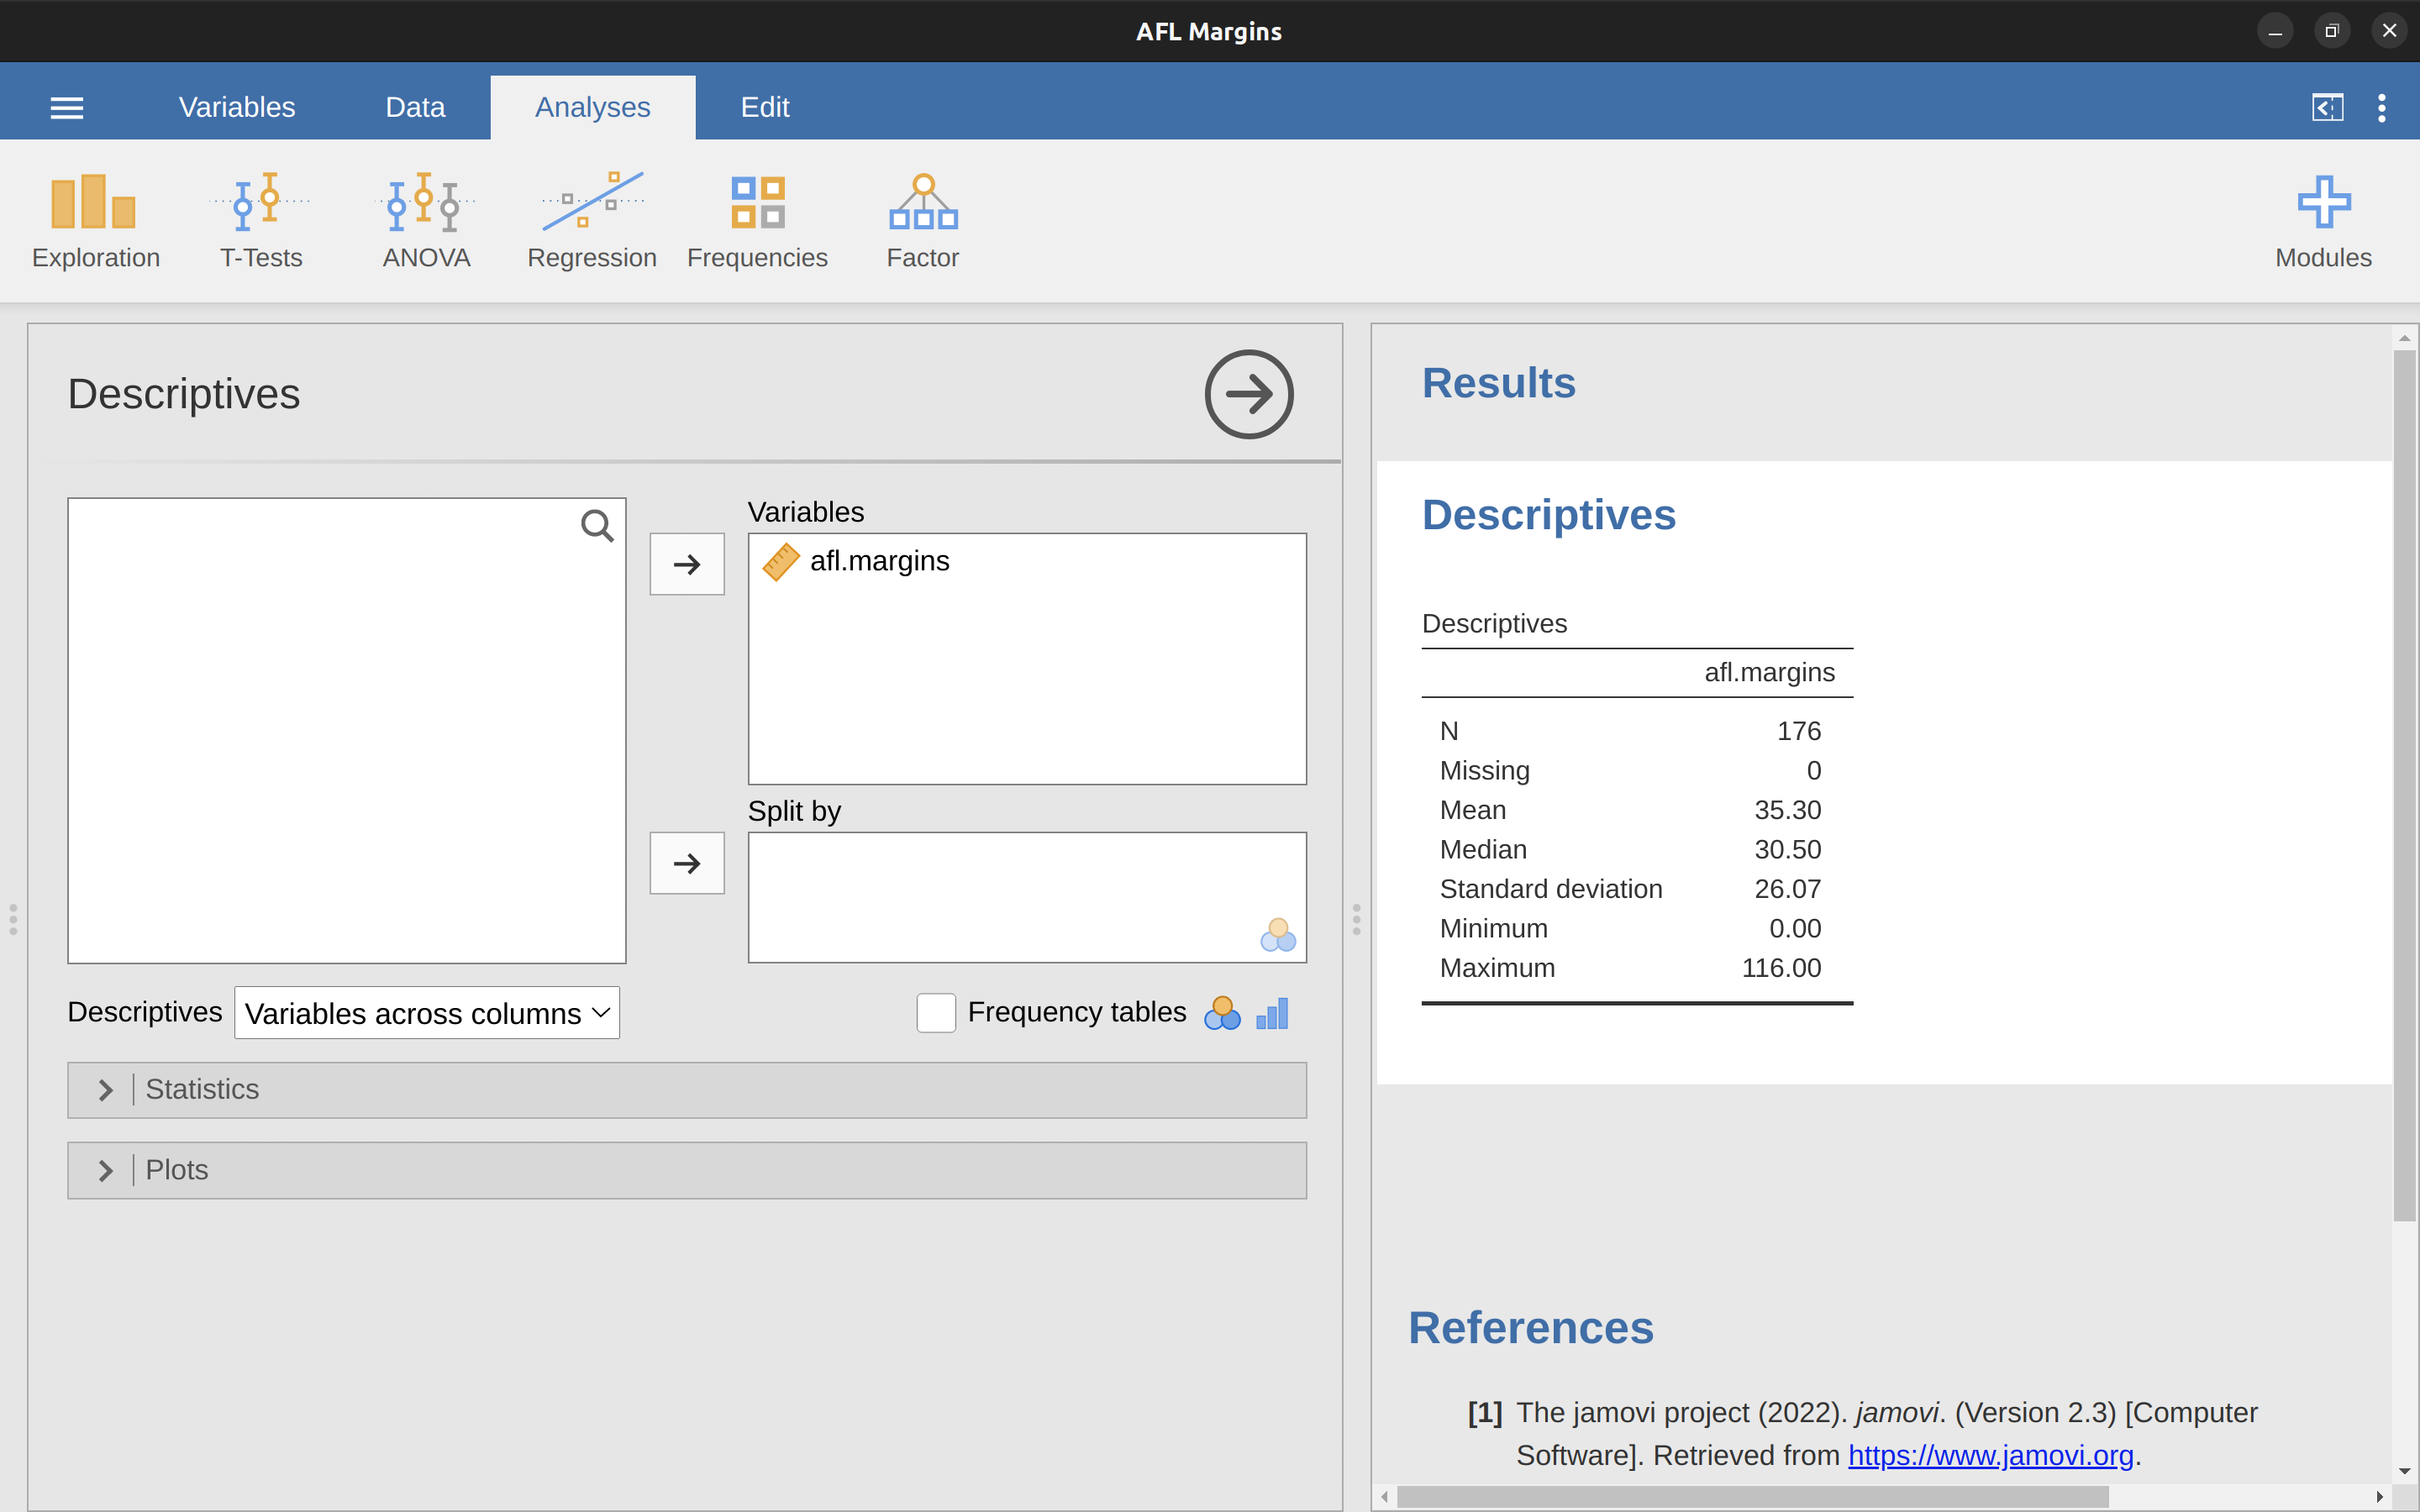
\includegraphics{./images/fig4-3.png} \hfill{}

\caption{\label{fig-fig4-3}Default descriptives for the AFL 2010 winning
margin data (the afl.margins variable)}

\end{figure}

As you can see in Figure~\ref{fig-fig4-3}, the mean value for the
afl.margins variable is 35.30. Other information presented includes the
total number of observations (N=176), the number of missing values
(none), and the Median, Minimum and Maximum values for the variable.

\hypertarget{the-median}{%
\subsection{The median}\label{the-median}}

The second measure of central tendency that people use a lot is the
\textbf{median}, and it's even easier to describe than the mean. The
median of a set of observations is just the middle value. As before
let's imagine we were interested only in the first 5 AFL winning
margins: \(56\), \(31\), \(56\), \(8\) and \(32\). To figure out the
median we sort these numbers into ascending order:

8, 31, \textbf{32}, 56, 56

From inspection, it's obvious that the median value of these 5
observations is 32 since that's the middle one in the sorted list (I've
put it in bold to make it even more obvious). Easy stuff. But what
should we do if we are interested in the first 6 games rather than the
first 5? Since the sixth game in the season had a winning margin of 14
points, our sorted list is now

8, \textbf{31}, \textbf{32}, 56, 56

and there are two middle numbers, 31 and 32. The median is defined as
the average of those two numbers, which is of course 31.5. As before,
it's very tedious to do this by hand when you've got lots of numbers. In
real life, of course, no-one actually calculates the median by sorting
the data and then looking for the middle value. In real life we use a
computer to do the heavy lifting for us, and jamovi has provided us with
a Median value of 30.50 for the afl.margins variable
(Figure~\ref{fig-fig4-3}).

\hypertarget{mean-or-median-whats-the-difference}{%
\subsection{Mean or median? What's the
difference?}\label{mean-or-median-whats-the-difference}}

Knowing how to calculate means and medians is only a part of the story.
You also need to understand what each one is saying about the data, and
what that implies for when you should use each one. This is illustrated
in Figure~\ref{fig-fig4-4}. The mean is kind of like the ``centre of
gravity'' of the data set, whereas the median is the ``middle value'' in
the data. What this implies, as far as which one you should use, depends
a little on what type of data you've got and what you're trying to
achieve. As a rough guide:

\begin{itemize}
\tightlist
\item
  If your data are nominal scale you probably shouldn't be using either
  the mean or the median. Both the mean and the median rely on the idea
  that the numbers assigned to values are meaningful. If the numbering
  scheme is arbitrary then it's probably best to use the
  \protect\hyperlink{sec-Mode}{Mode} instead.
\item
  If your data are ordinal scale you're more likely to want to use the
  median than the mean. The median only makes use of the order
  information in your data (i.e., which numbers are bigger) but doesn't
  depend on the precise numbers involved. That's exactly the situation
  that applies when your data are ordinal scale. The mean, on the other
  hand, makes use of the precise numeric values assigned to the
  observations, so it's not really appropriate for ordinal data.
\item
  For interval and ratio scale data either one is generally acceptable.
  Which one you pick depends a bit on what you're trying to achieve. The
  mean has the advantage that it uses all the information in the data
  (which is useful when you don't have a lot of data). But it's very
  sensitive to extreme, outlying values.
\end{itemize}

Let's expand on that last part a little. One consequence is that there
are systematic differences between the mean and the median when the
histogram is asymmetric (\protect\hyperlink{skew-and-kurtosis}{Skew and
kurtosis}). This is illustrated in Figure~\ref{fig-fig4-4}. Notice that
the median (right hand side) is located closer to the ``body'' of the
histogram, whereas the mean (left hand side) gets dragged towards the
``tail'' (where the extreme values are). To give a concrete example,
suppose Bob (income \$50,000), Kate (income \$60,000) and Jane (income
\$65,000) are sitting at a table. The average income at the table is
\$58,333 and the median income is \$60,000. Then Bill sits down with
them (income \$100,000,000). The average income has now jumped to
\$25,043,750 but the median rises only to \$62,500. If you're interested
in looking at the overall income at the table the mean might be the
right answer. But if you're interested in what counts as a typical
income at the table the median would be a better choice here.

\begin{figure}

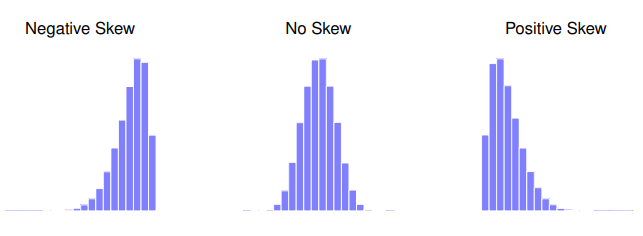
\includegraphics{./images/fig4-11.png} \hfill{}

\caption{\label{fig-fig4-4}An illustration of the difference between how
the mean and the median should be interpreted. The mean is basically the
`centre of gravity' of the data set. If you imagine that the histogram
of the data is a solid object, then the point on which you could balance
it (as if on a see-saw) is the mean. In contrast, the median is the
middle observation, with half of the observations smaller and half of
the observations larger}

\end{figure}

\hypertarget{sec-A-real-life-example}{%
\subsection{A real life example}\label{sec-A-real-life-example}}

To try to get a sense of why you need to pay attention to the
differences between the mean and the median let's consider a real life
example. Since I tend to mock journalists for their poor scientific and
statistical knowledge, I should give credit where credit is due. This is
an excellent article on the ABC news website\footnote{\url{www.abc.net.au/news/stories/2010/09/24/3021480.htm}}
from 24 September, 2010:

\begin{quote}
Senior Commonwealth Bank executives have travelled the world in the past
couple of weeks with a presentation showing how Australian house prices,
and the key price to income ratios, compare favourably with similar
countries. ``Housing affordability has actually been going sideways for
the last five to six years,'' said Craig James, the chief economist of
the bank's trading arm, CommSec.
\end{quote}

This probably comes as a huge surprise to anyone with a mortgage, or who
wants a mortgage, or pays rent, or isn't completely oblivious to what's
been going on in the Australian housing market over the last several
years. Back to the article:

\begin{quote}
CBA has waged its war against what it believes are housing doomsayers
with graphs, numbers and international comparisons. In its presentation,
the bank rejects arguments that Australia's housing is relatively
expensive compared to incomes. It says Australia's house price to
household income ratio of 5.6 in the major cities, and 4.3 nationwide,
is comparable to many other developed nations. It says San Francisco and
New York have ratios of 7, Auckland's is 6.7, and Vancouver comes in at
9.3.
\end{quote}

More excellent news! Except, the article goes on to make the observation
that:

\begin{quote}
Many analysts say that has led the bank to use misleading figures and
comparisons. If you go to page four of CBA's presentation and read the
source information at the bottom of the graph and table, you would
notice there is an additional source on the international comparison --
Demographia. However, if the Commonwealth Bank had also used
Demographia's analysis of Australia's house price to income ratio, it
would have come up with a figure closer to 9 rather than 5.6 or 4.3
\end{quote}

That's, um, a rather serious discrepancy. One group of people say 9,
another says 4-5. Should we just split the difference and say the truth
lies somewhere in between? Absolutely not! This is a situation where
there is a right answer and a wrong answer. Demographia is correct, and
the Commonwealth Bank is wrong. As the article points out:

\begin{quote}
{[}An{]} obvious problem with the Commonwealth Bank's domestic price to
income figures is they compare average incomes with median house prices
(unlike the Demographia figures that compare median incomes to median
prices). The median is the mid-point, effectively cutting out the highs
and lows, and that means the average is generally higher when it comes
to incomes and asset prices, because it includes the earnings of
Australia's wealthiest people. To put it another way: the Commonwealth
Bank's figures count Ralph Norris' multi-million dollar pay packet on
the income side, but not his (no doubt) very expensive house in the
property price figures, thus understating the house price to income
ratio for middle-income Australians.
\end{quote}

Couldn't have put it better myself. The way that Demographia calculated
the ratio is the right thing to do. The way that the Bank did it is
incorrect. As for why an extremely quantitatively sophisticated
organisation such as a major bank made such an elementary mistake,
well\ldots{} I can't say for sure since I have no special insight into
their thinking. But the article itself does happen to mention the
following facts, which may or may not be relevant:

\begin{quote}
{[}As{]} Australia's largest home lender, the Commonwealth Bank has one
of the biggest vested interests in house prices rising. It effectively
owns a massive swathe of Australian housing as security for its home
loans as well as many small business loans.
\end{quote}

My, my.

\hypertarget{sec-Mode}{%
\subsection{Mode}\label{sec-Mode}}

The mode of a sample is very simple. It is the value that occurs most
frequently. We can illustrate the mode using a different AFL variable:
who has played in the most finals? Open the aflsmall finalists file and
take a look at the afl.finalists variable, see Figure~\ref{fig-fig4-5}.
This variable contains the names of all 400 teams that played in all 200
finals matches played during the period 1987 to 2010.

What we could do is read through all 400 entries and count the number of
occasions on which each team name appears in our list of finalists,
thereby producing a \textbf{frequency table}. However, that would be
mindless and boring: exactly the sort of task that computers are great
at. So let's use jamovi to do this for us. Under `Exploration' -
`Descriptives' click the small check box labelled `Frequency tables' and
you should get something like Figure~\ref{fig-fig4-6}.

Now that we have our frequency table we can just look at it and see
that, over the 24 years for which we have data, Geelong has played in
more finals than any other team. Thus, the mode of the afl.finalists
data is ``Geelong''. We can see that Geelong (39 finals) played in more
finals than any other team during the 1987-2010 period. It's also worth
noting that in the `Descriptives' Table no results are calculated for
Mean, Median, Minimum or Maximum. This is because the afl.finalists
variable is a nominal text variable so it makes no sense to calculate
these values.

\begin{figure}

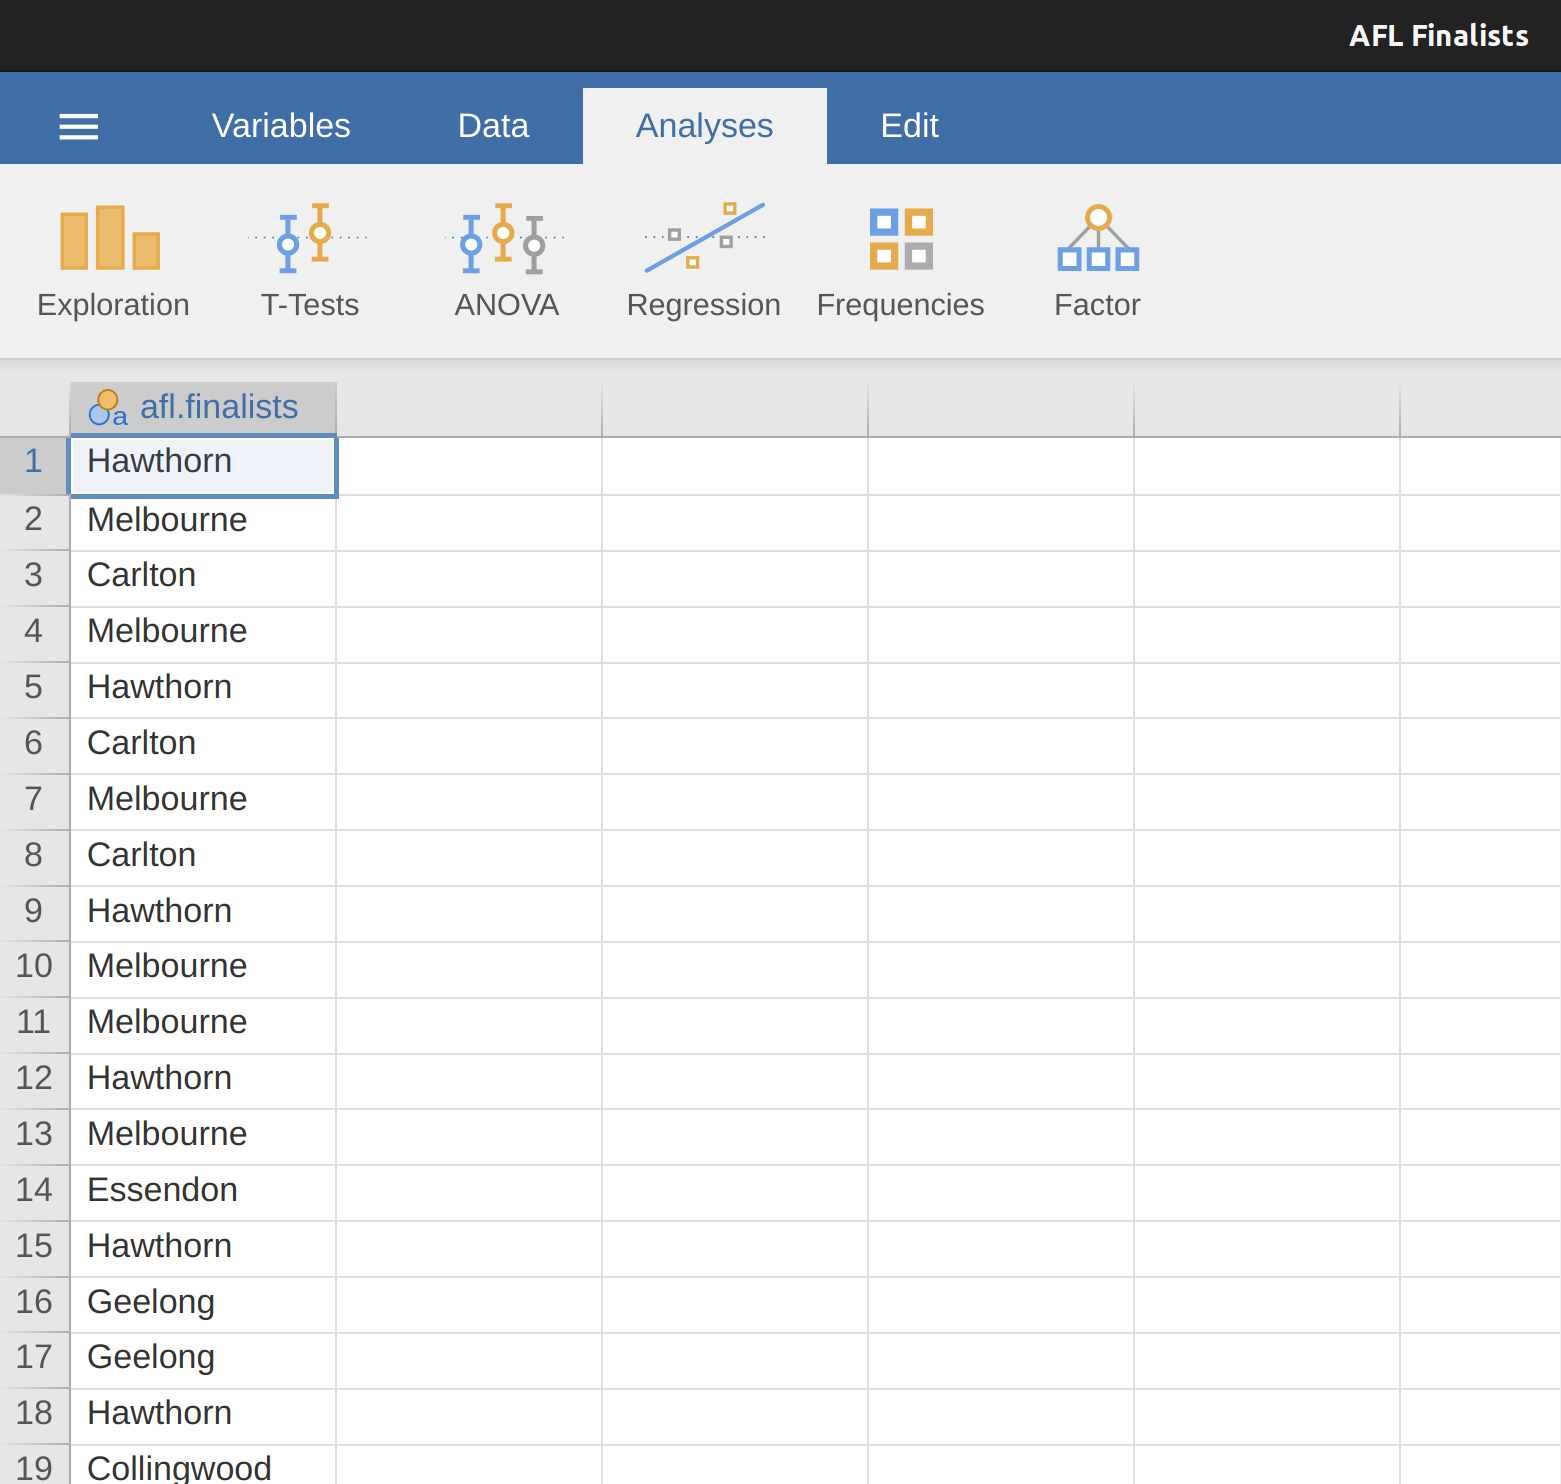
\includegraphics{./images/fig4-5.png} \hfill{}

\caption{\label{fig-fig4-5}A screenshot of jamovi showing the variables
stored in the aflsmall finalists.csv file}

\end{figure}

\begin{figure}

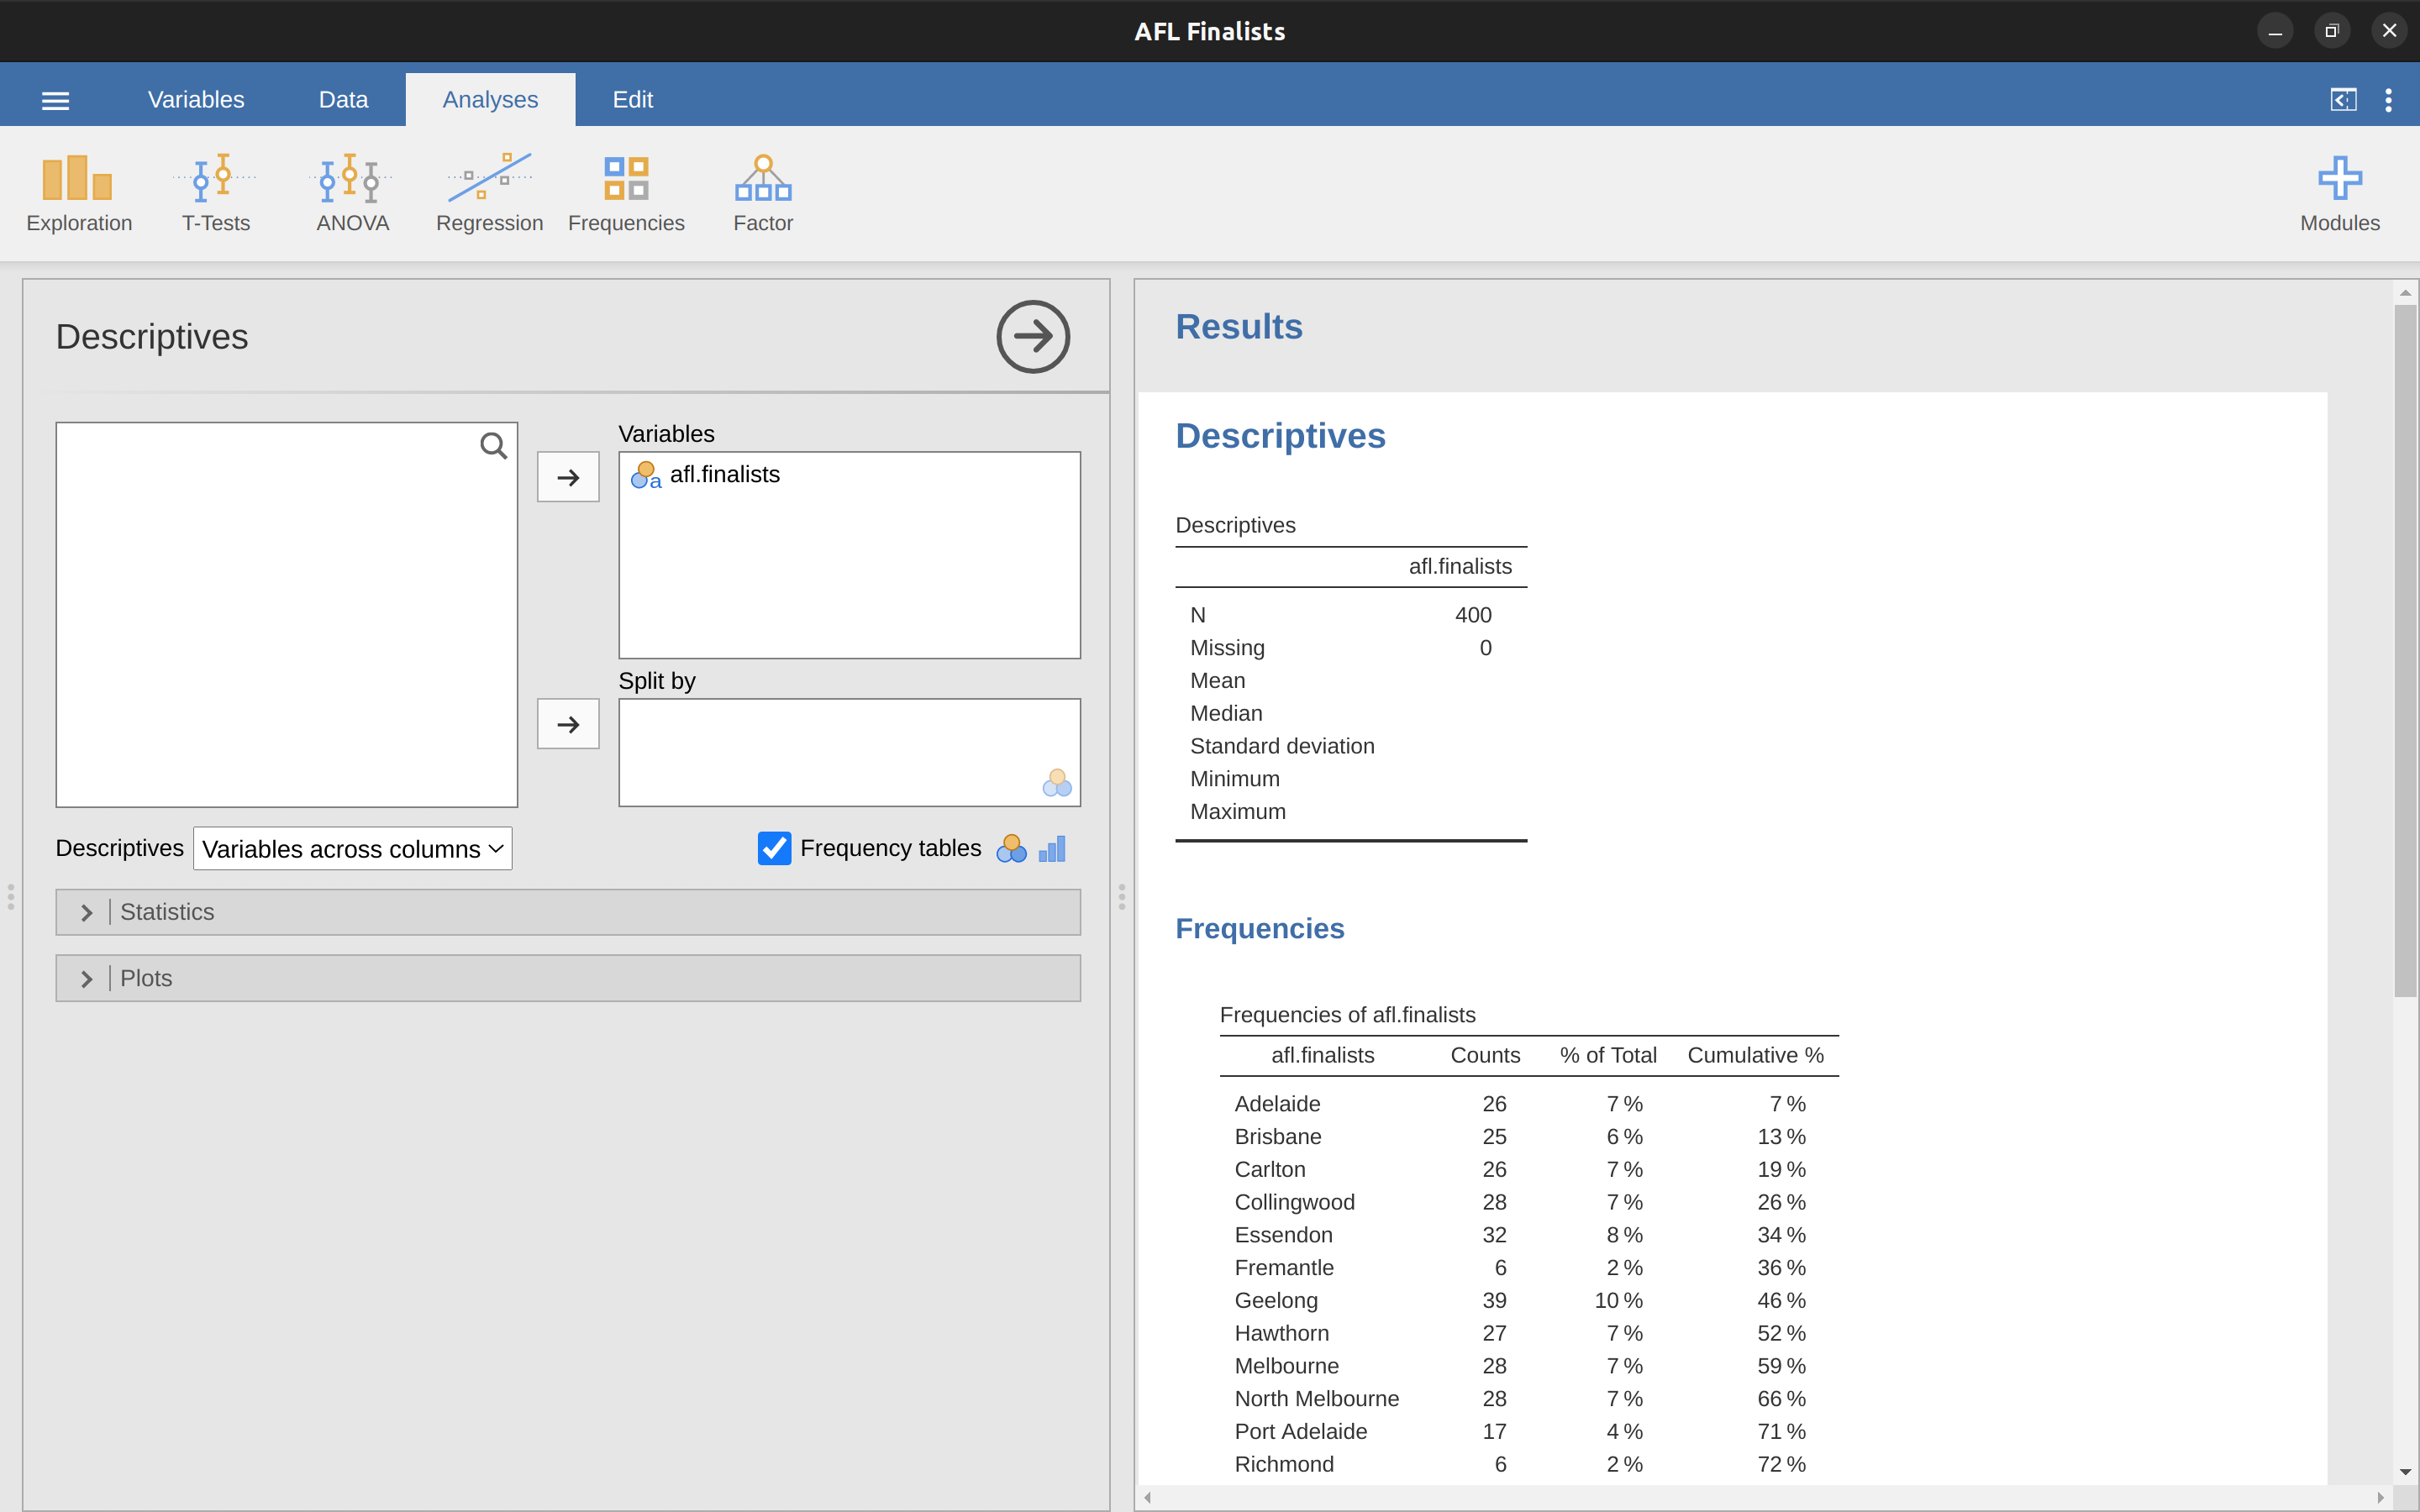
\includegraphics{./images/fig4-6.png} \hfill{}

\caption{\label{fig-fig4-6}A screenshot of jamovi showing the frequency
table for the afl.finalists variable}

\end{figure}

One last point to make regarding the mode. Whilst the mode is most often
calculated when you have nominal data, because means and medians are
useless for those sorts of variables, there are some situations in which
you really do want to know the mode of an ordinal, interval or ratio
scale variable. For instance, let's go back to our afl.margins variable.
This variable is clearly ratio scale (if it's not clear to you, it may
help to re-read Section~\ref{sec-Scales-of-measurement}), and so in most
situations the mean or the median is the measure of central tendency
that you want. But consider this scenario: a friend of yours is offering
a bet and they pick a football game at random. Without knowing who is
playing you have to guess the exact winning margin. If you guess
correctly you win \$50. If you don't you lose \$1. There are no
consolation prizes for ``almost'' getting the right answer. You have to
guess exactly the right margin. For this bet, the mean and the median
are completely useless to you. It is the mode that you should bet on. To
calculate the mode for the afl.margins variable in jamovi, go back to
that data set and on the `Exploration' - `Descriptives' screen you will
see you can expand the section marked `Statistics'. Click on the
checkbox marked `Mode' and you will see the modal value presented in the
`Descriptives' Table, as in Figure~\ref{fig-fig4-7}. So the 2010 data
suggest you should bet on a 3 point margin.

\begin{figure}

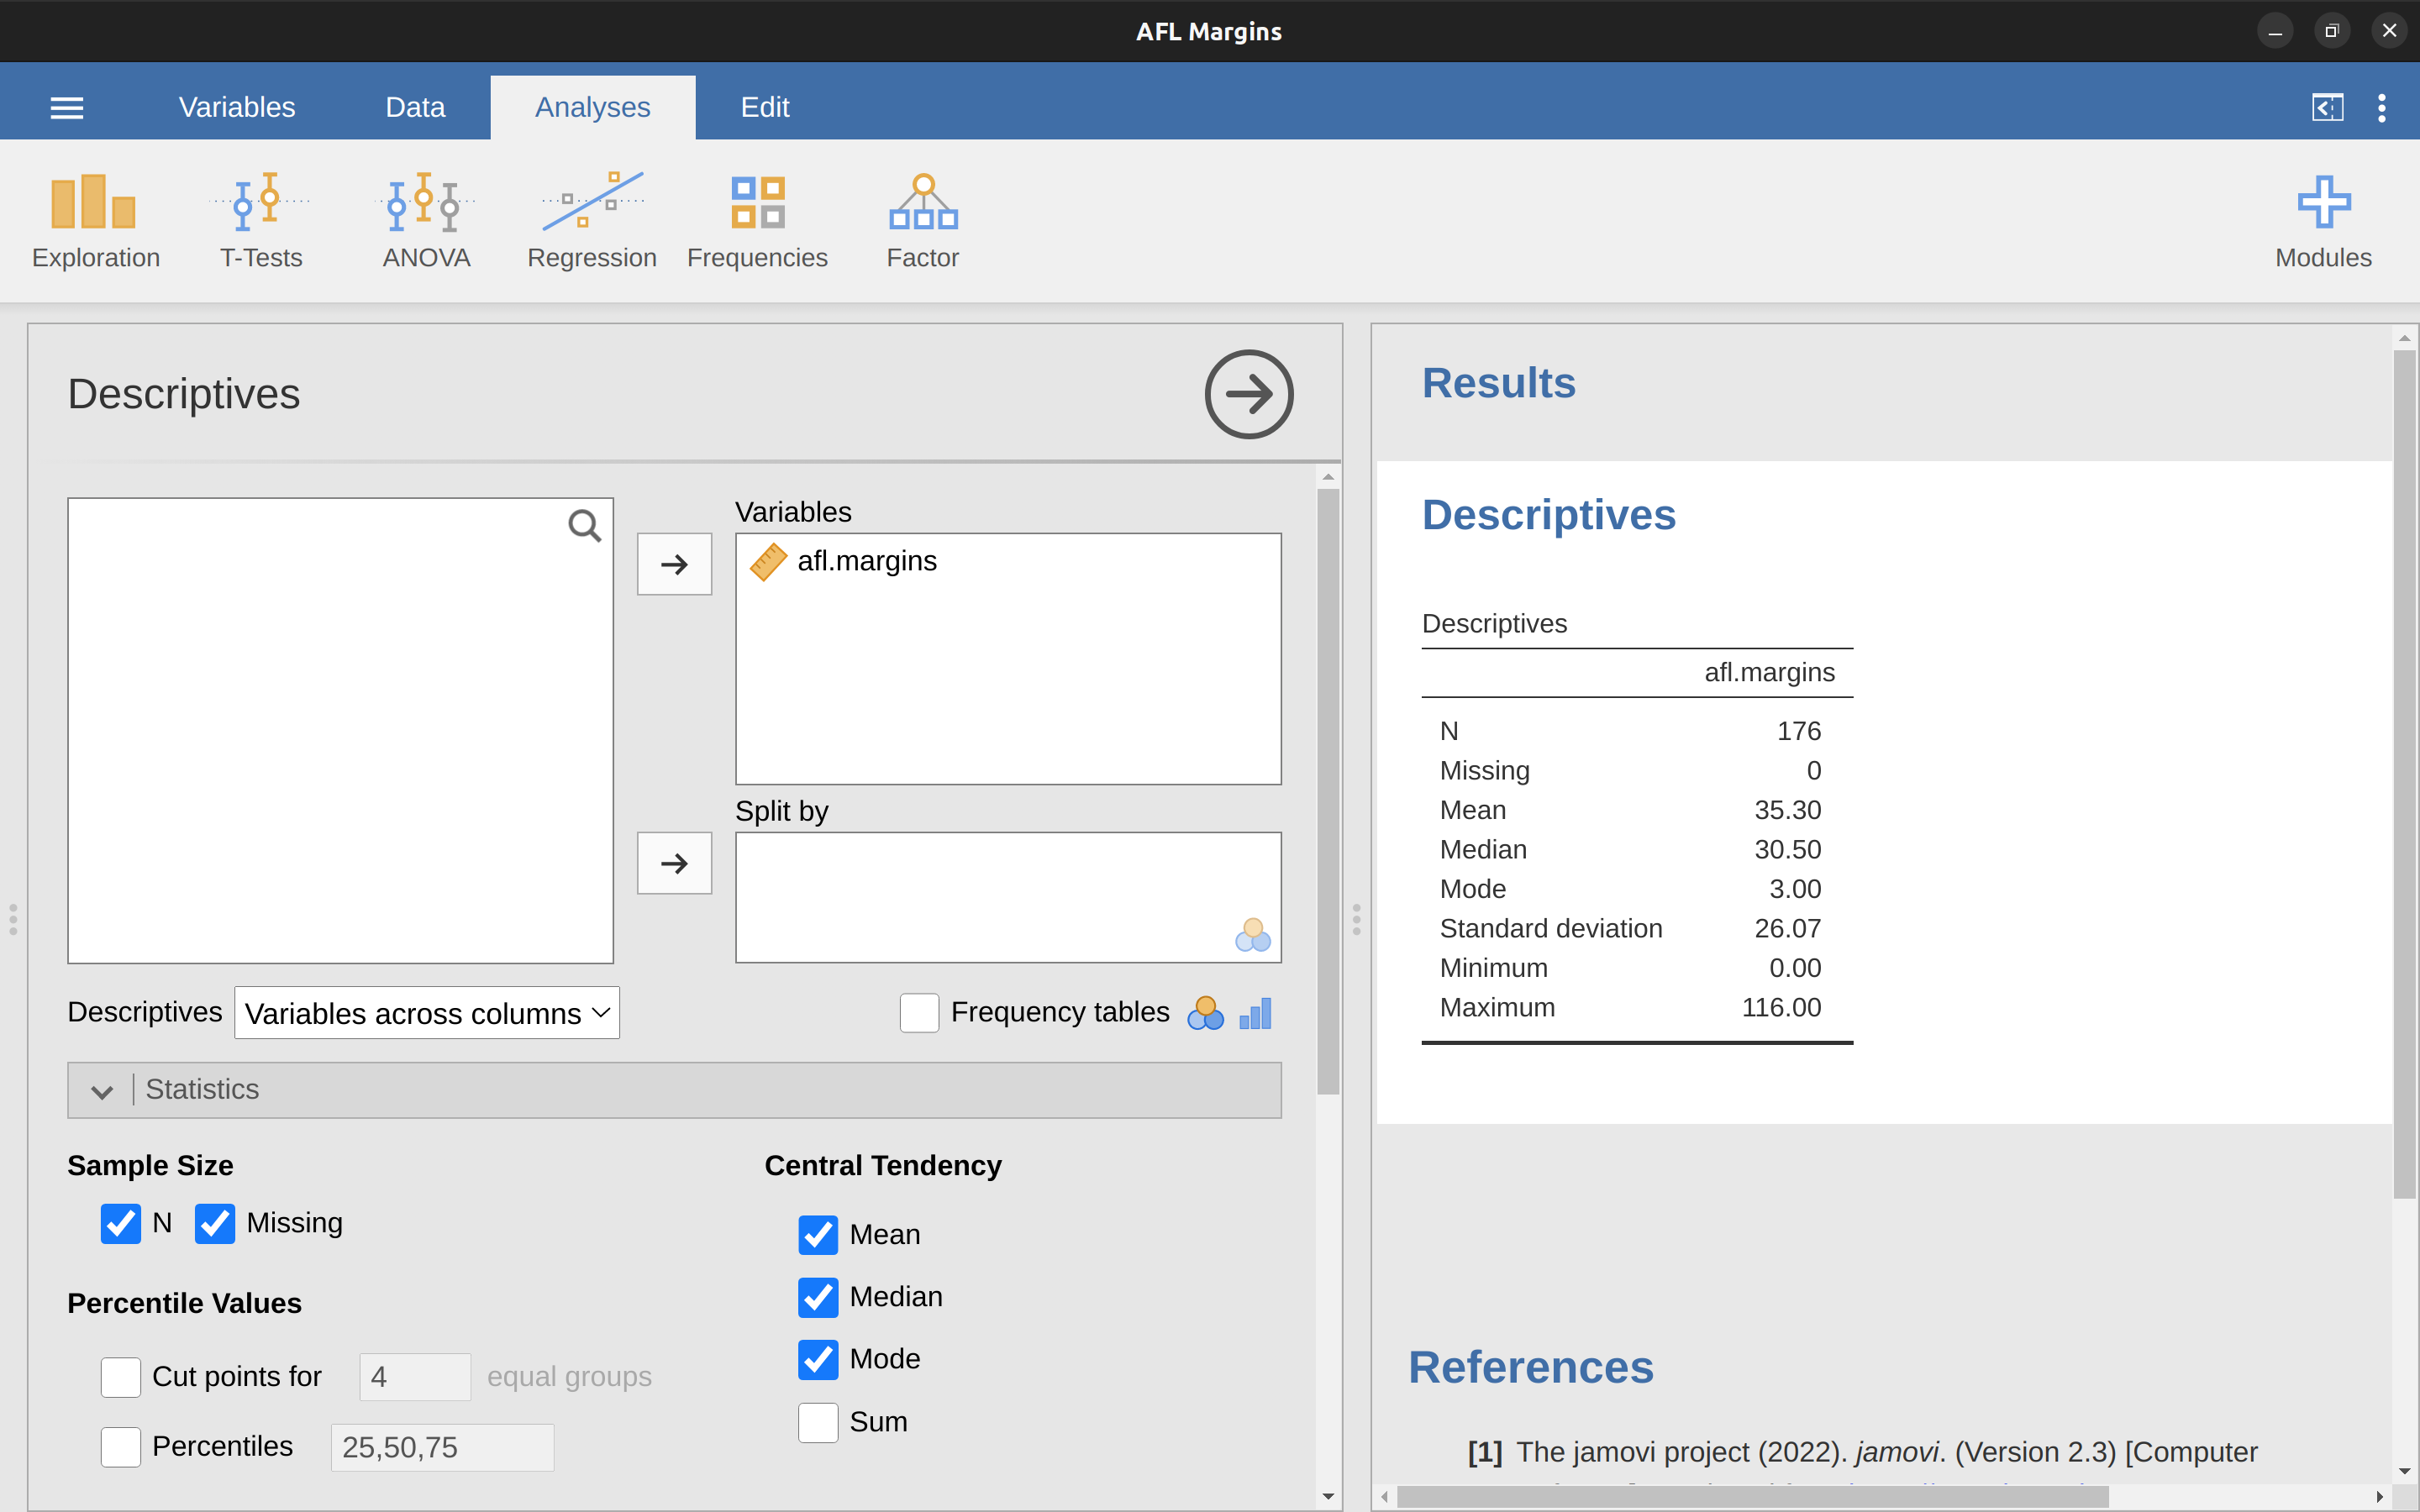
\includegraphics{./images/fig4-7.png} \hfill{}

\caption{\label{fig-fig4-7}A screenshot of jamovi showing the modal
value for the afl.margins variable}

\end{figure}

\hypertarget{sec-Measures-of-variability}{%
\section{Measures of variability}\label{sec-Measures-of-variability}}

The statistics that we've discussed so far all relate to central
tendency. That is, they all talk about which values are ``in the
middle'' or ``popular'' in the data. However, central tendency is not
the only type of summary statistic that we want to calculate. The second
thing that we really want is a measure of the \textbf{variability} of
the data. That is, how ``spread out'' are the data? How ``far'' away
from the mean or median do the observed values tend to be? For now,
let's assume that the data are interval or ratio scale, and we'll
continue to use the afl.margins data. We'll use this data to discuss
several different measures of spread, each with different strengths and
weaknesses.

\hypertarget{range}{%
\subsection{Range}\label{range}}

The statistics that we've discussed so far all relate to central
tendency. That is, they all talk about which values are ``in the
middle'' or ``popular'' in the data. However, central tendency is not
the only type of summary statistic that we want to calculate. The second
thing that we really want is a measure of the \textbf{variability} of
the data. That is, how ``spread out'' are the data? How ``far'' away
from the mean or median do the observed values tend to be? For now,
let's assume that the data are interval or ratio scale, and we'll
continue to use the afl.margins data. We'll use this data to discuss
several different measures of spread, each with different strengths and
weaknesses.

The \textbf{range} of a variable is very simple. It's the biggest value
minus the smallest value. For the AFL winning margins data the maximum
value is 116 and the minimum value is 0. Although the range is the
simplest way to quantify the notion of ``variability'', it's one of the
worst. Recall from our discussion of the mean that we want our summary
measure to be robust. If the data set has one or two extremely bad
values in it we'd like our statistics to not be unduly influenced by
these cases. For example, in a variable containing very extreme outliers

-100, 2, 3, 4, 5, 6, 7, 8, 9, 10

it is clear that the range is not robust. This variable has a range of
110 but if the outlier were removed we would have a range of only 8.

\hypertarget{interquartile-range}{%
\subsection{Interquartile range}\label{interquartile-range}}

The \textbf{interquartile range} (IQR) is like the range, but instead of
the difference between the biggest and smallest value the difference
between the 25th percentile and the 75th percentile is taken. If you
don't already know what a \textbf{percentile} is, the 10th percentile of
a data set is the smallest number x such that 10\% of the data is less
than x. In fact, we've already come across the idea. The median of a
data set is its 50th percentile! In jamovi you can easily specify the
25th, 50th and 75th percentiles by clicking the checkbox `Quartiles' in
the `Exploration' - `Descriptives' - `Statistics' screen.

And not surprisingly, in Figure~\ref{fig-fig4-8} the 50th percentile is
the same as the median value. And, by noting that
\(50.50 - 12.75 = 37.75\), we can see that the interquartile range for
the 2010 AFL winning margins data is 37.75. While it's obvious how to
interpret the range it's a little less obvious how to interpret the IQR.
The simplest way to think about it is like this: the interquartile range
is the range spanned by the ``middle half'' of the data. That is, one
quarter of the data falls below the 25th percentile and one quarter of
the data is above the 75th percentile, leaving the ``middle half'' of
the data lying in between the two. And the IQR is the range covered by
that middle half.

\begin{figure}

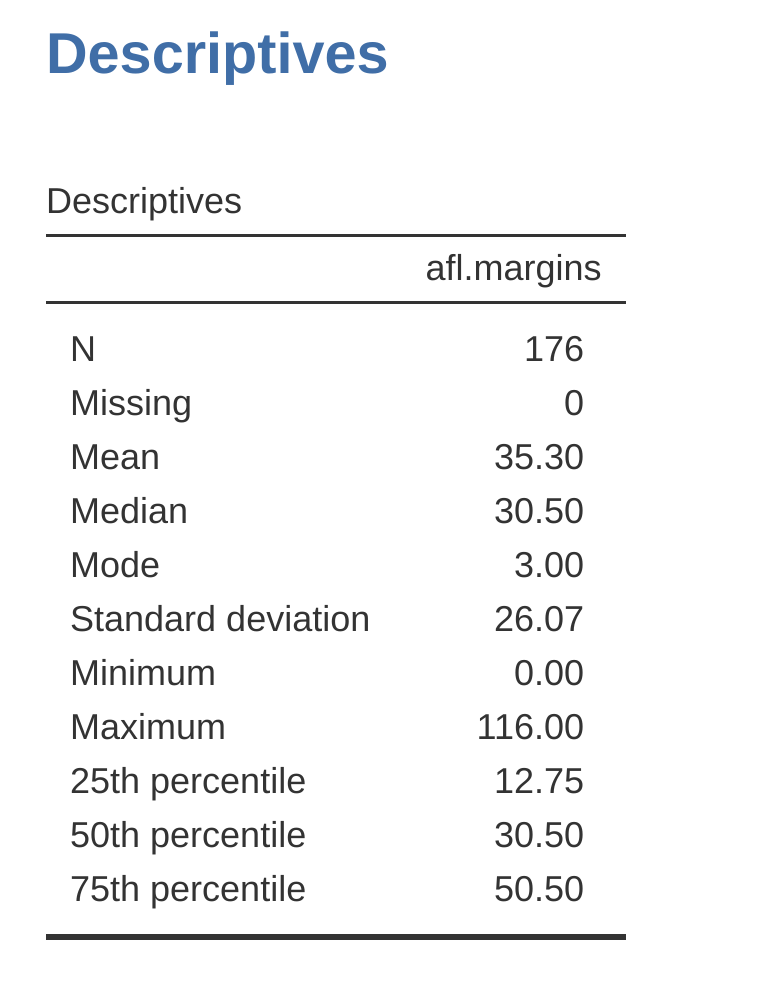
\includegraphics{./images/fig4-8.png} \hfill{}

\caption{\label{fig-fig4-8}A screenshot of jamovi showing the Quartiles
for the afl.margins variable}

\end{figure}

\hypertarget{mean-absolute-deviation}{%
\subsection{Mean absolute deviation}\label{mean-absolute-deviation}}

The two measures we've looked at so far, the range and the interquartile
range, both rely on the idea that we can measure the spread of the data
by looking at the percentiles of the data. However, this isn't the only
way to think about the problem. A different approach is to select a
meaningful reference point (usually the mean or the median) and then
report the ``typical'' deviations from that reference point. What do we
mean by ``typical'' deviation? Usually, this is the mean or median value
of these deviations. In practice, this leads to two different measures:
the ``mean absolute deviation'' (from the mean) and the ``median
absolute deviation'' (from the median). From what I've read, the measure
based on the median seems to be used in statistics and does seem to be
the better of the two. But to be honest I don't think I've seen it used
much in psychology. The measure based on the mean does occasionally show
up in psychology though. In this section I'll talk about the first one,
and I'll come back to talk about the second one later.

Since the previous paragraph might sound a little abstract, let's go
through the \textbf{mean absolute deviation} from the mean a little more
slowly. One useful thing about this measure is that the name actually
tells you exactly how to calculate it. Let's think about our AFL winning
margins data, and once again we'll start by pretending that there are
only 5 games in total, with winning margins of 56, 31, 56, 8 and 32.
Since our calculations rely on an examination of the deviation from some
reference point (in this case the mean), the first thing we need to
calculate is the mean, \(\bar{X}\). For these five observations, our
mean is \(\bar{X} = 36.6\). The next step is to convert each of our
observations \(X_i\) into a deviation score. We do this by calculating
the difference between the observation \(X_i\) and the mean \(\bar{X}\).
That is, the deviation score is defined to be \(X_i - \bar{X}\). For the
first observation in our sample, this is equal to \(56 - 36.6 = 19.4\).
Okay, that's simple enough. The next step in the process is to convert
these deviations to absolute deviations, and we do this by converting
any negative values to positive ones. Mathematically, we would denote
the absolute value of \(-3\) as \(\mid -3 \mid\), and so we say that
\(\mid -3 \mid = 3\). We use the absolute value here because we don't
really care whether the value is higher than the mean or lower than the
mean, we're just interested in how close it is to the mean. To help make
this process as obvious as possible, Table~\ref{tbl-tab4-2} shows these
calculations for all five observations.

\hypertarget{tbl-tab4-2}{}
 
  \providecommand{\huxb}[2]{\arrayrulecolor[RGB]{#1}\global\arrayrulewidth=#2pt}
  \providecommand{\huxvb}[2]{\color[RGB]{#1}\vrule width #2pt}
  \providecommand{\huxtpad}[1]{\rule{0pt}{#1}}
  \providecommand{\huxbpad}[1]{\rule[-#1]{0pt}{#1}}

\begin{table}[ht]
\caption{\label{tbl-tab4-2}Measures of variability }\tabularnewline

\begin{centerbox}
\begin{threeparttable}
\setlength{\tabcolsep}{0pt}
\begin{tabularx}{0.9\textwidth}{p{0.18\textwidth} p{0.18\textwidth} p{0.18\textwidth} p{0.18\textwidth} p{0.18\textwidth}}


\hhline{>{\huxb{0, 0, 0}{0.4}}->{\huxb{0, 0, 0}{0.4}}->{\huxb{0, 0, 0}{0.4}}->{\huxb{0, 0, 0}{0.4}}->{\huxb{0, 0, 0}{0.4}}-}
\arrayrulecolor{black}

\multicolumn{1}{!{\huxvb{0, 0, 0}{0}}p{0.18\textwidth}!{\huxvb{0, 0, 0}{0}}}{\cellcolor[RGB]{242, 242, 242}\hspace{0pt}\parbox[b]{0.18\textwidth-0pt-6pt}{\huxtpad{6pt + 1em}\centering \textbf{English}\huxbpad{6pt}}} &
\multicolumn{1}{p{0.18\textwidth}!{\huxvb{0, 0, 0}{0}}}{\cellcolor[RGB]{242, 242, 242}\hspace{6pt}\parbox[b]{0.18\textwidth-6pt-6pt}{\huxtpad{6pt + 1em}\centering \textbf{notation}\huxbpad{6pt}}} &
\multicolumn{1}{p{0.18\textwidth}!{\huxvb{0, 0, 0}{0}}}{\cellcolor[RGB]{242, 242, 242}\hspace{6pt}\parbox[b]{0.18\textwidth-6pt-6pt}{\huxtpad{6pt + 1em}\centering \textbf{value}\huxbpad{6pt}}} &
\multicolumn{1}{p{0.18\textwidth}!{\huxvb{0, 0, 0}{0}}}{\cellcolor[RGB]{242, 242, 242}\hspace{6pt}\parbox[b]{0.18\textwidth-6pt-6pt}{\huxtpad{6pt + 1em}\centering \textbf{deviation from mean}\huxbpad{6pt}}} &
\multicolumn{1}{p{0.18\textwidth}!{\huxvb{0, 0, 0}{0}}}{\cellcolor[RGB]{242, 242, 242}\hspace{6pt}\parbox[b]{0.18\textwidth-6pt-0pt}{\huxtpad{6pt + 1em}\centering \textbf{absolute deviation}\huxbpad{6pt}}} \tabularnewline[-0.5pt]


\hhline{>{\huxb{0, 0, 0}{0.4}}->{\huxb{0, 0, 0}{0.4}}->{\huxb{0, 0, 0}{0.4}}->{\huxb{0, 0, 0}{0.4}}->{\huxb{0, 0, 0}{0.4}}-}
\arrayrulecolor{black}

\multicolumn{1}{!{\huxvb{0, 0, 0}{0}}p{0.18\textwidth}!{\huxvb{0, 0, 0}{0}}}{\hspace{0pt}\parbox[b]{0.18\textwidth-0pt-6pt}{\huxtpad{6pt + 1em}\centering notation:\huxbpad{6pt}}} &
\multicolumn{1}{p{0.18\textwidth}!{\huxvb{0, 0, 0}{0}}}{\hspace{6pt}\parbox[b]{0.18\textwidth-6pt-6pt}{\huxtpad{6pt + 1em}\centering \(i\)\huxbpad{6pt}}} &
\multicolumn{1}{p{0.18\textwidth}!{\huxvb{0, 0, 0}{0}}}{\hspace{6pt}\parbox[b]{0.18\textwidth-6pt-6pt}{\huxtpad{6pt + 1em}\centering \(X_i\)\huxbpad{6pt}}} &
\multicolumn{1}{p{0.18\textwidth}!{\huxvb{0, 0, 0}{0}}}{\hspace{6pt}\parbox[b]{0.18\textwidth-6pt-6pt}{\huxtpad{6pt + 1em}\centering \(X_i - \bar{X} \)\huxbpad{6pt}}} &
\multicolumn{1}{p{0.18\textwidth}!{\huxvb{0, 0, 0}{0}}}{\hspace{6pt}\parbox[b]{0.18\textwidth-6pt-0pt}{\huxtpad{6pt + 1em}\centering \( \mid X_i - \bar{X} \mid \)\huxbpad{6pt}}} \tabularnewline[-0.5pt]


\hhline{}
\arrayrulecolor{black}

\multicolumn{1}{!{\huxvb{0, 0, 0}{0}}p{0.18\textwidth}!{\huxvb{0, 0, 0}{0}}}{\cellcolor[RGB]{242, 242, 242}\hspace{0pt}\parbox[b]{0.18\textwidth-0pt-6pt}{\huxtpad{6pt + 1em}\centering \huxbpad{6pt}}} &
\multicolumn{1}{p{0.18\textwidth}!{\huxvb{0, 0, 0}{0}}}{\cellcolor[RGB]{242, 242, 242}\hspace{6pt}\parbox[b]{0.18\textwidth-6pt-6pt}{\huxtpad{6pt + 1em}\centering 1\huxbpad{6pt}}} &
\multicolumn{1}{p{0.18\textwidth}!{\huxvb{0, 0, 0}{0}}}{\cellcolor[RGB]{242, 242, 242}\hspace{6pt}\parbox[b]{0.18\textwidth-6pt-6pt}{\huxtpad{6pt + 1em}\centering 56\huxbpad{6pt}}} &
\multicolumn{1}{p{0.18\textwidth}!{\huxvb{0, 0, 0}{0}}}{\cellcolor[RGB]{242, 242, 242}\hspace{6pt}\parbox[b]{0.18\textwidth-6pt-6pt}{\huxtpad{6pt + 1em}\centering 19.4\huxbpad{6pt}}} &
\multicolumn{1}{p{0.18\textwidth}!{\huxvb{0, 0, 0}{0}}}{\cellcolor[RGB]{242, 242, 242}\hspace{6pt}\parbox[b]{0.18\textwidth-6pt-0pt}{\huxtpad{6pt + 1em}\centering 19.4\huxbpad{6pt}}} \tabularnewline[-0.5pt]


\hhline{}
\arrayrulecolor{black}

\multicolumn{1}{!{\huxvb{0, 0, 0}{0}}p{0.18\textwidth}!{\huxvb{0, 0, 0}{0}}}{\hspace{0pt}\parbox[b]{0.18\textwidth-0pt-6pt}{\huxtpad{6pt + 1em}\centering \huxbpad{6pt}}} &
\multicolumn{1}{p{0.18\textwidth}!{\huxvb{0, 0, 0}{0}}}{\hspace{6pt}\parbox[b]{0.18\textwidth-6pt-6pt}{\huxtpad{6pt + 1em}\centering 2\huxbpad{6pt}}} &
\multicolumn{1}{p{0.18\textwidth}!{\huxvb{0, 0, 0}{0}}}{\hspace{6pt}\parbox[b]{0.18\textwidth-6pt-6pt}{\huxtpad{6pt + 1em}\centering 31\huxbpad{6pt}}} &
\multicolumn{1}{p{0.18\textwidth}!{\huxvb{0, 0, 0}{0}}}{\hspace{6pt}\parbox[b]{0.18\textwidth-6pt-6pt}{\huxtpad{6pt + 1em}\centering -5.6\huxbpad{6pt}}} &
\multicolumn{1}{p{0.18\textwidth}!{\huxvb{0, 0, 0}{0}}}{\hspace{6pt}\parbox[b]{0.18\textwidth-6pt-0pt}{\huxtpad{6pt + 1em}\centering 5.6\huxbpad{6pt}}} \tabularnewline[-0.5pt]


\hhline{}
\arrayrulecolor{black}

\multicolumn{1}{!{\huxvb{0, 0, 0}{0}}p{0.18\textwidth}!{\huxvb{0, 0, 0}{0}}}{\cellcolor[RGB]{242, 242, 242}\hspace{0pt}\parbox[b]{0.18\textwidth-0pt-6pt}{\huxtpad{6pt + 1em}\centering \huxbpad{6pt}}} &
\multicolumn{1}{p{0.18\textwidth}!{\huxvb{0, 0, 0}{0}}}{\cellcolor[RGB]{242, 242, 242}\hspace{6pt}\parbox[b]{0.18\textwidth-6pt-6pt}{\huxtpad{6pt + 1em}\centering 3\huxbpad{6pt}}} &
\multicolumn{1}{p{0.18\textwidth}!{\huxvb{0, 0, 0}{0}}}{\cellcolor[RGB]{242, 242, 242}\hspace{6pt}\parbox[b]{0.18\textwidth-6pt-6pt}{\huxtpad{6pt + 1em}\centering 56\huxbpad{6pt}}} &
\multicolumn{1}{p{0.18\textwidth}!{\huxvb{0, 0, 0}{0}}}{\cellcolor[RGB]{242, 242, 242}\hspace{6pt}\parbox[b]{0.18\textwidth-6pt-6pt}{\huxtpad{6pt + 1em}\centering 19.4\huxbpad{6pt}}} &
\multicolumn{1}{p{0.18\textwidth}!{\huxvb{0, 0, 0}{0}}}{\cellcolor[RGB]{242, 242, 242}\hspace{6pt}\parbox[b]{0.18\textwidth-6pt-0pt}{\huxtpad{6pt + 1em}\centering 19.4\huxbpad{6pt}}} \tabularnewline[-0.5pt]


\hhline{}
\arrayrulecolor{black}

\multicolumn{1}{!{\huxvb{0, 0, 0}{0}}p{0.18\textwidth}!{\huxvb{0, 0, 0}{0}}}{\hspace{0pt}\parbox[b]{0.18\textwidth-0pt-6pt}{\huxtpad{6pt + 1em}\centering \huxbpad{6pt}}} &
\multicolumn{1}{p{0.18\textwidth}!{\huxvb{0, 0, 0}{0}}}{\hspace{6pt}\parbox[b]{0.18\textwidth-6pt-6pt}{\huxtpad{6pt + 1em}\centering 4\huxbpad{6pt}}} &
\multicolumn{1}{p{0.18\textwidth}!{\huxvb{0, 0, 0}{0}}}{\hspace{6pt}\parbox[b]{0.18\textwidth-6pt-6pt}{\huxtpad{6pt + 1em}\centering 8\huxbpad{6pt}}} &
\multicolumn{1}{p{0.18\textwidth}!{\huxvb{0, 0, 0}{0}}}{\hspace{6pt}\parbox[b]{0.18\textwidth-6pt-6pt}{\huxtpad{6pt + 1em}\centering -28.6\huxbpad{6pt}}} &
\multicolumn{1}{p{0.18\textwidth}!{\huxvb{0, 0, 0}{0}}}{\hspace{6pt}\parbox[b]{0.18\textwidth-6pt-0pt}{\huxtpad{6pt + 1em}\centering 28.6\huxbpad{6pt}}} \tabularnewline[-0.5pt]


\hhline{}
\arrayrulecolor{black}

\multicolumn{1}{!{\huxvb{0, 0, 0}{0}}p{0.18\textwidth}!{\huxvb{0, 0, 0}{0}}}{\cellcolor[RGB]{242, 242, 242}\hspace{0pt}\parbox[b]{0.18\textwidth-0pt-6pt}{\huxtpad{6pt + 1em}\centering \huxbpad{6pt}}} &
\multicolumn{1}{p{0.18\textwidth}!{\huxvb{0, 0, 0}{0}}}{\cellcolor[RGB]{242, 242, 242}\hspace{6pt}\parbox[b]{0.18\textwidth-6pt-6pt}{\huxtpad{6pt + 1em}\centering 5\huxbpad{6pt}}} &
\multicolumn{1}{p{0.18\textwidth}!{\huxvb{0, 0, 0}{0}}}{\cellcolor[RGB]{242, 242, 242}\hspace{6pt}\parbox[b]{0.18\textwidth-6pt-6pt}{\huxtpad{6pt + 1em}\centering 32\huxbpad{6pt}}} &
\multicolumn{1}{p{0.18\textwidth}!{\huxvb{0, 0, 0}{0}}}{\cellcolor[RGB]{242, 242, 242}\hspace{6pt}\parbox[b]{0.18\textwidth-6pt-6pt}{\huxtpad{6pt + 1em}\centering -4.6\huxbpad{6pt}}} &
\multicolumn{1}{p{0.18\textwidth}!{\huxvb{0, 0, 0}{0}}}{\cellcolor[RGB]{242, 242, 242}\hspace{6pt}\parbox[b]{0.18\textwidth-6pt-0pt}{\huxtpad{6pt + 1em}\centering 4.6\huxbpad{6pt}}} \tabularnewline[-0.5pt]


\hhline{>{\huxb{0, 0, 0}{0.4}}->{\huxb{0, 0, 0}{0.4}}->{\huxb{0, 0, 0}{0.4}}->{\huxb{0, 0, 0}{0.4}}->{\huxb{0, 0, 0}{0.4}}-}
\arrayrulecolor{black}
\end{tabularx} 

\end{threeparttable}\par\end{centerbox}

\end{table}
 

Now that we have calculated the absolute deviation score for every
observation in the data set, all that we have to do to calculate the
mean of these scores. Let's do that:

\[
\frac{19.4 + 5.6 + 19.4 + 28.6 + 4.6}{5} = 15.52
\]

And we're done. The mean absolute deviation for these five scores is
15.52.

{[}Additional technical detail\footnote{However, whilst our calculations
  for this little example are at an end, we do have a couple of things
  left to talk about. First, we should really try to write down a proper
  mathematical formula. But in order do to this I need some mathematical
  notation to refer to the mean absolute deviation. Irritatingly, ``mean
  absolute deviation'' and ``median absolute deviation'' have the same
  acronym (MAD), which leads to a certain amount of ambiguity so I'd
  better come up with something different for the mean absolute
  deviation. Sigh. What I'll do is use AAD instead, short for average
  absolute deviation. Now that we have some unambiguous notation, here's
  the formula that describes what we just
  calculated:\[AAD(X) =\frac{1}{N} \sum_{i=1}^{N} \mid X_i - \bar{X} \mid = 15.52\]}{]}

\hypertarget{variance}{%
\subsection{Variance}\label{variance}}

Although the average absolute deviation measure has its uses, it's not
the best measure of variability to use. From a purely mathematical
perspective there are some solid reasons to prefer squared deviations
rather than absolute deviations. If we do that we obtain a measure
called the \textbf{variance}, which has a lot of really nice statistical
properties that I'm going to ignore,\footnote{Well, I will very briefly
  mention the one that I think is coolest, for a very particular
  definition of ``cool'', that is. Variances are additive. Here's what
  that means. Suppose I have two variables \(X\) and \(Y\) , whose
  variances are \(Var(X)\) and \(Var(Y)\) respectively. Now imagine I
  want to define a new variable Z that is the sum of the two,
  \(Z = X + Y\) . As it turns out, the variance of \(Z\) is equal to
  \(Var(X) + Var(Y)\). This is a very useful property, but it's not true
  of the other measures that I talk about in this section.} and one
massive psychological flaw that I'm going to make a big deal out of in a
moment. The variance of a data set \(X\) is sometimes written as Var(
\(X\) ), but it's more commonly denoted \(s^2\) (the reason for this
will become clearer shortly).

{[}Additional technical detail\footnote{The formula that we use to
  calculate the variance of a set of observations is as follows:
  \[VAR(X) =\frac{1}{N} \sum_{i=1}^{N} ( X_i - \bar{X} )^2
  \] As you can see, it's basically the same formula that we used to
  calculate the average absolute deviation, except that instead of using
  ``absolute deviations'' we use ``squared deviations''. It is for this
  reason that the variance is sometimes referred to as the ``mean square
  deviation''.}{]}

Now that we've got the basic idea, let's have a look at a concrete
example. Once again, let's use the first five AFL games as our data. If
we follow the same approach that we took last time, we end up with the
information shown in Table~\ref{tbl-tab4-3}.

\hypertarget{tbl-tab4-3}{}
 
  \providecommand{\huxb}[2]{\arrayrulecolor[RGB]{#1}\global\arrayrulewidth=#2pt}
  \providecommand{\huxvb}[2]{\color[RGB]{#1}\vrule width #2pt}
  \providecommand{\huxtpad}[1]{\rule{0pt}{#1}}
  \providecommand{\huxbpad}[1]{\rule[-#1]{0pt}{#1}}

\begin{table}[ht]
\caption{\label{tbl-tab4-3}Measures of variability for the first five AFL games }\tabularnewline

\begin{centerbox}
\begin{threeparttable}
\setlength{\tabcolsep}{0pt}
\begin{tabularx}{0.9\textwidth}{p{0.18\textwidth} p{0.18\textwidth} p{0.18\textwidth} p{0.18\textwidth} p{0.18\textwidth}}


\hhline{>{\huxb{0, 0, 0}{0.4}}->{\huxb{0, 0, 0}{0.4}}->{\huxb{0, 0, 0}{0.4}}->{\huxb{0, 0, 0}{0.4}}->{\huxb{0, 0, 0}{0.4}}-}
\arrayrulecolor{black}

\multicolumn{1}{!{\huxvb{0, 0, 0}{0}}p{0.18\textwidth}!{\huxvb{0, 0, 0}{0}}}{\cellcolor[RGB]{242, 242, 242}\hspace{0pt}\parbox[b]{0.18\textwidth-0pt-6pt}{\huxtpad{6pt + 1em}\centering \textbf{English}\huxbpad{6pt}}} &
\multicolumn{1}{p{0.18\textwidth}!{\huxvb{0, 0, 0}{0}}}{\cellcolor[RGB]{242, 242, 242}\hspace{6pt}\parbox[b]{0.18\textwidth-6pt-6pt}{\huxtpad{6pt + 1em}\centering \textbf{maths:}\huxbpad{6pt}}} &
\multicolumn{1}{p{0.18\textwidth}!{\huxvb{0, 0, 0}{0}}}{\cellcolor[RGB]{242, 242, 242}\hspace{6pt}\parbox[b]{0.18\textwidth-6pt-6pt}{\huxtpad{6pt + 1em}\centering \textbf{value}\huxbpad{6pt}}} &
\multicolumn{1}{p{0.18\textwidth}!{\huxvb{0, 0, 0}{0}}}{\cellcolor[RGB]{242, 242, 242}\hspace{6pt}\parbox[b]{0.18\textwidth-6pt-6pt}{\huxtpad{6pt + 1em}\centering \textbf{deviation from mean}\huxbpad{6pt}}} &
\multicolumn{1}{p{0.18\textwidth}!{\huxvb{0, 0, 0}{0}}}{\cellcolor[RGB]{242, 242, 242}\hspace{6pt}\parbox[b]{0.18\textwidth-6pt-0pt}{\huxtpad{6pt + 1em}\centering \textbf{absolute deviation}\huxbpad{6pt}}} \tabularnewline[-0.5pt]


\hhline{>{\huxb{0, 0, 0}{0.4}}->{\huxb{0, 0, 0}{0.4}}->{\huxb{0, 0, 0}{0.4}}->{\huxb{0, 0, 0}{0.4}}->{\huxb{0, 0, 0}{0.4}}-}
\arrayrulecolor{black}

\multicolumn{1}{!{\huxvb{0, 0, 0}{0}}p{0.18\textwidth}!{\huxvb{0, 0, 0}{0}}}{\hspace{0pt}\parbox[b]{0.18\textwidth-0pt-6pt}{\huxtpad{6pt + 1em}\centering notation:\huxbpad{6pt}}} &
\multicolumn{1}{p{0.18\textwidth}!{\huxvb{0, 0, 0}{0}}}{\hspace{6pt}\parbox[b]{0.18\textwidth-6pt-6pt}{\huxtpad{6pt + 1em}\centering \(i\)\huxbpad{6pt}}} &
\multicolumn{1}{p{0.18\textwidth}!{\huxvb{0, 0, 0}{0}}}{\hspace{6pt}\parbox[b]{0.18\textwidth-6pt-6pt}{\huxtpad{6pt + 1em}\centering \(X_i\)\huxbpad{6pt}}} &
\multicolumn{1}{p{0.18\textwidth}!{\huxvb{0, 0, 0}{0}}}{\hspace{6pt}\parbox[b]{0.18\textwidth-6pt-6pt}{\huxtpad{6pt + 1em}\centering \(X_i - \bar{X} \)\huxbpad{6pt}}} &
\multicolumn{1}{p{0.18\textwidth}!{\huxvb{0, 0, 0}{0}}}{\hspace{6pt}\parbox[b]{0.18\textwidth-6pt-0pt}{\huxtpad{6pt + 1em}\centering \( ( X_i - \bar{X} )^2 \)\huxbpad{6pt}}} \tabularnewline[-0.5pt]


\hhline{}
\arrayrulecolor{black}

\multicolumn{1}{!{\huxvb{0, 0, 0}{0}}p{0.18\textwidth}!{\huxvb{0, 0, 0}{0}}}{\cellcolor[RGB]{242, 242, 242}\hspace{0pt}\parbox[b]{0.18\textwidth-0pt-6pt}{\huxtpad{6pt + 1em}\centering \huxbpad{6pt}}} &
\multicolumn{1}{p{0.18\textwidth}!{\huxvb{0, 0, 0}{0}}}{\cellcolor[RGB]{242, 242, 242}\hspace{6pt}\parbox[b]{0.18\textwidth-6pt-6pt}{\huxtpad{6pt + 1em}\centering 1\huxbpad{6pt}}} &
\multicolumn{1}{p{0.18\textwidth}!{\huxvb{0, 0, 0}{0}}}{\cellcolor[RGB]{242, 242, 242}\hspace{6pt}\parbox[b]{0.18\textwidth-6pt-6pt}{\huxtpad{6pt + 1em}\centering 56\huxbpad{6pt}}} &
\multicolumn{1}{p{0.18\textwidth}!{\huxvb{0, 0, 0}{0}}}{\cellcolor[RGB]{242, 242, 242}\hspace{6pt}\parbox[b]{0.18\textwidth-6pt-6pt}{\huxtpad{6pt + 1em}\centering 19.4\huxbpad{6pt}}} &
\multicolumn{1}{p{0.18\textwidth}!{\huxvb{0, 0, 0}{0}}}{\cellcolor[RGB]{242, 242, 242}\hspace{6pt}\parbox[b]{0.18\textwidth-6pt-0pt}{\huxtpad{6pt + 1em}\centering 376.36\huxbpad{6pt}}} \tabularnewline[-0.5pt]


\hhline{}
\arrayrulecolor{black}

\multicolumn{1}{!{\huxvb{0, 0, 0}{0}}p{0.18\textwidth}!{\huxvb{0, 0, 0}{0}}}{\hspace{0pt}\parbox[b]{0.18\textwidth-0pt-6pt}{\huxtpad{6pt + 1em}\centering \huxbpad{6pt}}} &
\multicolumn{1}{p{0.18\textwidth}!{\huxvb{0, 0, 0}{0}}}{\hspace{6pt}\parbox[b]{0.18\textwidth-6pt-6pt}{\huxtpad{6pt + 1em}\centering 2\huxbpad{6pt}}} &
\multicolumn{1}{p{0.18\textwidth}!{\huxvb{0, 0, 0}{0}}}{\hspace{6pt}\parbox[b]{0.18\textwidth-6pt-6pt}{\huxtpad{6pt + 1em}\centering 31\huxbpad{6pt}}} &
\multicolumn{1}{p{0.18\textwidth}!{\huxvb{0, 0, 0}{0}}}{\hspace{6pt}\parbox[b]{0.18\textwidth-6pt-6pt}{\huxtpad{6pt + 1em}\centering -5.6\huxbpad{6pt}}} &
\multicolumn{1}{p{0.18\textwidth}!{\huxvb{0, 0, 0}{0}}}{\hspace{6pt}\parbox[b]{0.18\textwidth-6pt-0pt}{\huxtpad{6pt + 1em}\centering 31.36\huxbpad{6pt}}} \tabularnewline[-0.5pt]


\hhline{}
\arrayrulecolor{black}

\multicolumn{1}{!{\huxvb{0, 0, 0}{0}}p{0.18\textwidth}!{\huxvb{0, 0, 0}{0}}}{\cellcolor[RGB]{242, 242, 242}\hspace{0pt}\parbox[b]{0.18\textwidth-0pt-6pt}{\huxtpad{6pt + 1em}\centering \huxbpad{6pt}}} &
\multicolumn{1}{p{0.18\textwidth}!{\huxvb{0, 0, 0}{0}}}{\cellcolor[RGB]{242, 242, 242}\hspace{6pt}\parbox[b]{0.18\textwidth-6pt-6pt}{\huxtpad{6pt + 1em}\centering 3\huxbpad{6pt}}} &
\multicolumn{1}{p{0.18\textwidth}!{\huxvb{0, 0, 0}{0}}}{\cellcolor[RGB]{242, 242, 242}\hspace{6pt}\parbox[b]{0.18\textwidth-6pt-6pt}{\huxtpad{6pt + 1em}\centering 56\huxbpad{6pt}}} &
\multicolumn{1}{p{0.18\textwidth}!{\huxvb{0, 0, 0}{0}}}{\cellcolor[RGB]{242, 242, 242}\hspace{6pt}\parbox[b]{0.18\textwidth-6pt-6pt}{\huxtpad{6pt + 1em}\centering 19.4\huxbpad{6pt}}} &
\multicolumn{1}{p{0.18\textwidth}!{\huxvb{0, 0, 0}{0}}}{\cellcolor[RGB]{242, 242, 242}\hspace{6pt}\parbox[b]{0.18\textwidth-6pt-0pt}{\huxtpad{6pt + 1em}\centering 376.36\huxbpad{6pt}}} \tabularnewline[-0.5pt]


\hhline{}
\arrayrulecolor{black}

\multicolumn{1}{!{\huxvb{0, 0, 0}{0}}p{0.18\textwidth}!{\huxvb{0, 0, 0}{0}}}{\hspace{0pt}\parbox[b]{0.18\textwidth-0pt-6pt}{\huxtpad{6pt + 1em}\centering \huxbpad{6pt}}} &
\multicolumn{1}{p{0.18\textwidth}!{\huxvb{0, 0, 0}{0}}}{\hspace{6pt}\parbox[b]{0.18\textwidth-6pt-6pt}{\huxtpad{6pt + 1em}\centering 4\huxbpad{6pt}}} &
\multicolumn{1}{p{0.18\textwidth}!{\huxvb{0, 0, 0}{0}}}{\hspace{6pt}\parbox[b]{0.18\textwidth-6pt-6pt}{\huxtpad{6pt + 1em}\centering 8\huxbpad{6pt}}} &
\multicolumn{1}{p{0.18\textwidth}!{\huxvb{0, 0, 0}{0}}}{\hspace{6pt}\parbox[b]{0.18\textwidth-6pt-6pt}{\huxtpad{6pt + 1em}\centering -28.6\huxbpad{6pt}}} &
\multicolumn{1}{p{0.18\textwidth}!{\huxvb{0, 0, 0}{0}}}{\hspace{6pt}\parbox[b]{0.18\textwidth-6pt-0pt}{\huxtpad{6pt + 1em}\centering 817.96\huxbpad{6pt}}} \tabularnewline[-0.5pt]


\hhline{}
\arrayrulecolor{black}

\multicolumn{1}{!{\huxvb{0, 0, 0}{0}}p{0.18\textwidth}!{\huxvb{0, 0, 0}{0}}}{\cellcolor[RGB]{242, 242, 242}\hspace{0pt}\parbox[b]{0.18\textwidth-0pt-6pt}{\huxtpad{6pt + 1em}\centering \huxbpad{6pt}}} &
\multicolumn{1}{p{0.18\textwidth}!{\huxvb{0, 0, 0}{0}}}{\cellcolor[RGB]{242, 242, 242}\hspace{6pt}\parbox[b]{0.18\textwidth-6pt-6pt}{\huxtpad{6pt + 1em}\centering 5\huxbpad{6pt}}} &
\multicolumn{1}{p{0.18\textwidth}!{\huxvb{0, 0, 0}{0}}}{\cellcolor[RGB]{242, 242, 242}\hspace{6pt}\parbox[b]{0.18\textwidth-6pt-6pt}{\huxtpad{6pt + 1em}\centering 32\huxbpad{6pt}}} &
\multicolumn{1}{p{0.18\textwidth}!{\huxvb{0, 0, 0}{0}}}{\cellcolor[RGB]{242, 242, 242}\hspace{6pt}\parbox[b]{0.18\textwidth-6pt-6pt}{\huxtpad{6pt + 1em}\centering -4.6\huxbpad{6pt}}} &
\multicolumn{1}{p{0.18\textwidth}!{\huxvb{0, 0, 0}{0}}}{\cellcolor[RGB]{242, 242, 242}\hspace{6pt}\parbox[b]{0.18\textwidth-6pt-0pt}{\huxtpad{6pt + 1em}\centering 21.16\huxbpad{6pt}}} \tabularnewline[-0.5pt]


\hhline{>{\huxb{0, 0, 0}{0.4}}->{\huxb{0, 0, 0}{0.4}}->{\huxb{0, 0, 0}{0.4}}->{\huxb{0, 0, 0}{0.4}}->{\huxb{0, 0, 0}{0.4}}-}
\arrayrulecolor{black}
\end{tabularx} 

\end{threeparttable}\par\end{centerbox}

\end{table}
 

That last column contains all of our squared deviations, so all we have
to do is average them. If we do that by hand, i.e.~using a calculator,
we end up with a variance of \(324.64\). Exciting, isn't it? For the
moment, let's ignore the burning question that you're all probably
thinking (i.e., what the heck does a variance of \(324.64\) actually
mean?) and instead talk a bit more about how to do the calculations in
jamovi, because this will reveal something very weird. Start a new
jamovi session by clicking on the main menu button (three horizontal
lines in the top left corner and selecting `New'. Now type in the first
five values from the afl.margins data set in column A (\(56\), \(31\),
\(56\), \(8\), \(32\). Change the variable type to `Continuous' and
under `Descriptives' click the `Variance' check box, and you get the
same values for variance as the one we calculated by hand (\(324.64\)).
No, wait, you get a completely different answer (\(405.80\)) - see
Figure~\ref{fig-fig4-9}. That's just weird. Is jamovi broken? Is this a
typo? Am I an idiot?

\begin{figure}

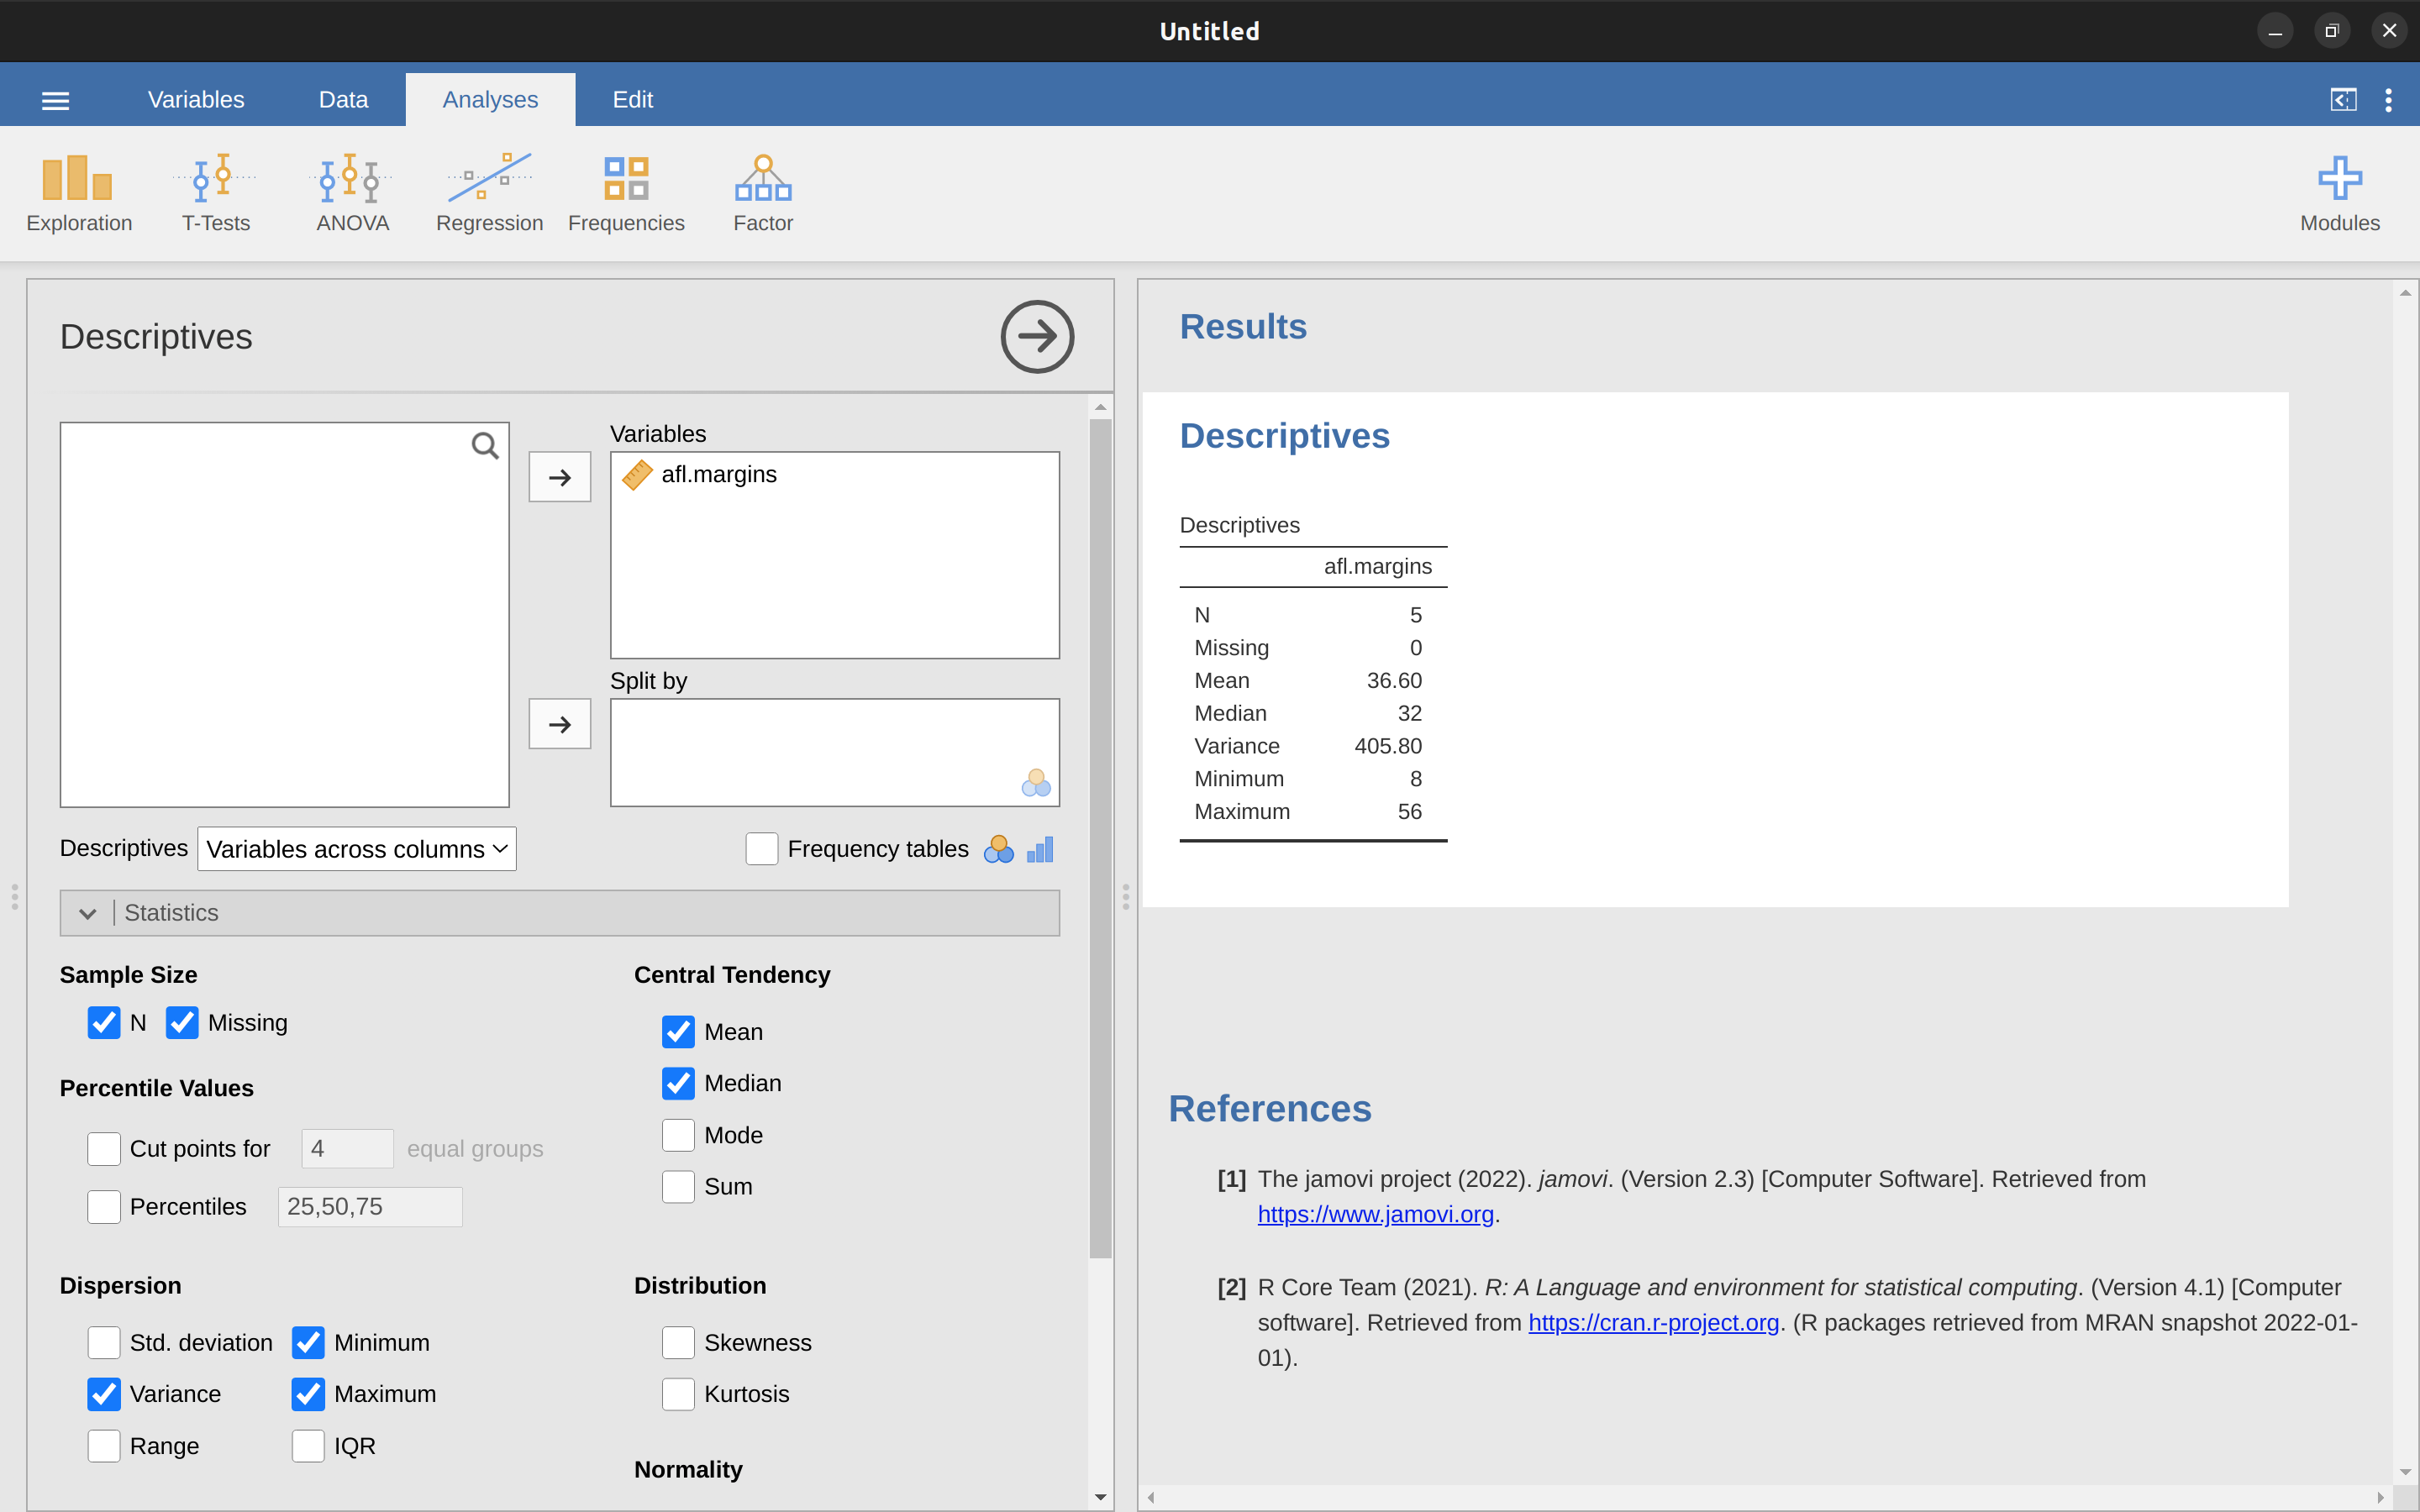
\includegraphics{./images/fig4-9.png} \hfill{}

\caption{\label{fig-fig4-9}A screenshot of jamovi showing the Variance
for the first 5 values of the afl.margins variable}

\end{figure}

As it happens, the answer is no.\footnote{With the possible exception of
  the third question.} It's not a typo, and jamovi is not making a
mistake. In fact, it's very simple to explain what jamovi is doing here,
but slightly trickier to explain why jamovi is doing it. So let's start
with the ``what''. What jamovi is doing is evaluating a slightly
different formula to the one I showed you above. Instead of averaging
the squared deviations, which requires you to divide by the number of
data points N, jamovi has chosen to divide by \(N - 1\).

{[}Additional technical detail\footnote{In other words, the formula that
  jamovi is using is this one:
  \[\frac{1}{N-1} \sum_{i=1}^{N} ( X_i - \bar{X} )^2\]}{]}

So that's the \emph{what}. The real question is why jamovi is dividing
by \(N - 1\) and not by \(N\). After all, the variance is supposed to be
the mean squared deviation, right? So shouldn't we be dividing by N, the
actual number of observations in the sample? Well, yes, we should.
However, as we'll discuss in the chapter on
Chapter~\ref{sec-Estimating-unknown-quantities-from-a-sample}, there's a
subtle distinction between ``describing a sample'' and ``making guesses
about the population from which the sample came''. Up to this point,
it's been a distinction without a difference. Regardless of whether
you're describing a sample or drawing inferences about the population,
the mean is calculated exactly the same way. Not so for the variance, or
the standard deviation, or for many other measures besides. What I
outlined to you initially (i.e., take the actual average, and thus
divide by \(N\)) assumes that you literally intend to calculate the
variance of the sample. Most of the time, however, you're not terribly
interested in the sample in and of itself. Rather, the sample exists to
tell you something about the world. If so, you're actually starting to
move away from calculating a ``sample statistic'' and towards the idea
of estimating a ``population parameter''. However, I'm getting ahead of
myself. For now, let's just take it on faith that jamovi knows what it's
doing, and we'll revisit the question later on when we talk about
estimation in
Chapter~\ref{sec-Estimating-unknown-quantities-from-a-sample}.

Okay, one last thing. This section so far has read a bit like a mystery
novel. I've shown you how to calculate the variance, described the weird
``\(N - 1\)'' thing that jamovi does and hinted at the reason why it's
there, but I haven't mentioned the single most important thing. How do
you interpret the variance? Descriptive statistics are supposed to
describe things, after all, and right now the variance is really just a
gibberish number. Unfortunately, the reason why I haven't given you the
human-friendly interpretation of the variance is that there really isn't
one. This is the most serious problem with the variance. Although it has
some elegant mathematical properties that suggest that it really is a
fundamental quantity for expressing variation, it's completely useless
if you want to communicate with an actual human. Variances are
completely uninterpretable in terms of the original variable! All the
numbers have been squared and they don't mean anything anymore. This is
a huge issue. For instance, according to Table~\ref{tbl-tab4-3}, the
margin in game 1 was ``376.36 points-squared higher than the average
margin''. This is \emph{exactly} as stupid as it sounds, and so when we
calculate a variance of \(324.64\) we're in the same situation. I've
watched a lot of footy games, and at no time has anyone ever referred to
``points squared''. It's not a real unit of measurement, and since the
variance is expressed in terms of this gibberish unit, it is totally
meaningless to a human.

\hypertarget{sec-Standard-deviation}{%
\subsection{Standard deviation}\label{sec-Standard-deviation}}

Okay, suppose that you like the idea of using the variance because of
those nice mathematical properties that I haven't talked about, but
since you're a human and not a robot you'd like to have a measure that
is expressed in the same units as the data itself (i.e., points, not
points squared). What should you do? The solution to the problem is
obvious! Take the square root of the variance, known as the
\textbf{standard deviation}, also called the ``root mean squared
deviation'', or RMSD. This solves our problem fairly neatly. Whilst
nobody has a clue what ``a variance of 324.68 points-squared'' really
means, it's much easier to understand ``a standard deviation of 18.01
points'' since it's expressed in the original units. It is traditional
to refer to the standard deviation of a sample of data as s, though
``sd'' and ``std dev.'' are also used at times.

{[}Additional technical detail\footnote{Because the standard deviation
  is equal to the square root of the variance, you probably won't be
  surprised to see that the formula is:
  \[s=\sqrt{\frac{1}{N} \sum_{i=1}^{N} ( X_i - \bar{X} )^2 }\] and in
  jamovi there is a check box for `Std. deviation' right above the check
  box for `Variance'. Selecting this gives a value of \(26.07\) for the
  standard deviation.}{]}

However, as you might have guessed from our discussion of the variance,
what jamovi actually calculates is slightly different to the formula
given above. Just like the we saw with the variance, what jamovi
calculates is a version that divides by \(N - 1\) rather than \(N\).

{[}Additional technical detail\footnote{For reasons that will make sense
  when we return to this topic in
  Chapter~\ref{sec-Estimating-unknown-quantities-from-a-sample} I'll
  refer to this new quantity as \(\hat{\sigma}\) (read as: ``sigma
  hat''), and the formula for this is:
  \[\hat{\sigma}=\sqrt{\frac{1}{N-1} \sum_{i=1}^{N} ( X_i - \bar{X} )^2}\]}{]}

Interpreting standard deviations is slightly more complex. Because the
standard deviation is derived from the variance, and the variance is a
quantity that has little to no meaning that makes sense to us humans,
the standard deviation doesn't have a simple interpretation. As a
consequence, most of us just rely on a simple rule of thumb. In general,
you should expect 68\% of the data to fall within 1 standard deviation
of the mean, 95\% of the data to fall within 2 standard deviation of the
mean, and 99.7\% of the data to fall within 3 standard deviations of the
mean. This rule tends to work pretty well most of the time, but it's not
exact. It's actually calculated based on an assumption that the
histogram is symmetric and ``bell shaped''. As you can tell from looking
at the AFL winning margins histogram in Figure~\ref{fig-fig4-2}, this
isn't exactly true of our data! Even so, the rule is approximately
correct. As it turns out, 65.3\% of the AFL margins data fall within one
standard deviation of the mean. This is shown visually in
Figure~\ref{fig-fig4-10}.

\hypertarget{which-measure-to-use}{%
\subsection{Which measure to use?}\label{which-measure-to-use}}

We've discussed quite a few measures of spread: range, IQR, mean
absolute deviation, variance and standard deviation; and hinted at their
strengths and weaknesses. Here's a quick summary:

\begin{itemize}
\tightlist
\item
  \emph{Range}. Gives you the full spread of the data. It's very
  vulnerable to outliers and as a consequence it isn't often used unless
  you have good reasons to care about the extremes in the data.
\item
  \emph{Interquartile range}. Tells you where the ``middle half'' of the
  data sits. It's pretty robust and complements the median nicely. This
  is used a lot.
\item
  \emph{Mean absolute deviation}. Tells you how far ``on average'' the
  observations are from the mean. It's very interpretable but has a few
  minor issues (not discussed here) that make it less attractive to
  statisticians than the standard deviation. Used sometimes, but not
  often.
\item
  \emph{Variance}. Tells you the average squared deviation from the
  mean. It's mathematically elegant and is probably the ``right'' way to
  describe variation around the mean, but it's completely
  uninterpretable because it doesn't use the same units as the data.
  Almost never used except as a mathematical tool, but it's buried
  ``under the hood'' of a very large number of statistical tools.
\item
  \emph{Standard deviation}. This is the square root of the variance.
  It's fairly elegant mathematically and it's expressed in the same
  units as the data so it can be interpreted pretty well. In situations
  where the mean is the measure of central tendency, this is the
  default. This is by far the most popular measure of variation.
\end{itemize}

In short, the IQR and the standard deviation are easily the two most
common measures used to report the variability of the data. But there
are situations in which the others are used. I've described all of them
in this book because there's a fair chance you'll run into most of these
somewhere.

\begin{figure}

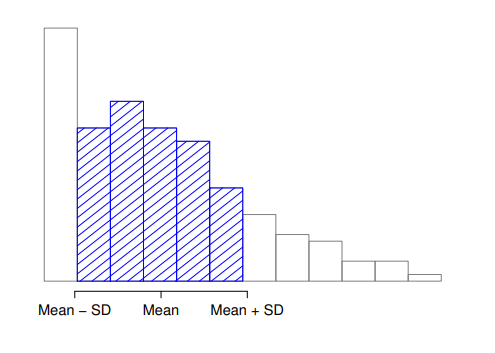
\includegraphics{./images/fig4-10.png} \hfill{}

\caption{\label{fig-fig4-10}An illustration of the standard deviation
from the AFL winning margins data. The shaded bars in the histogram show
how much of the data fall within one standard deviation of the mean. In
this case, 65.3\% of the data set lies within this range, which is
pretty consistent with the `approximately 68\% rule' discussed in the
main text}

\end{figure}

\hypertarget{skew-and-kurtosis}{%
\section{Skew and kurtosis}\label{skew-and-kurtosis}}

There are two more descriptive statistics that you will sometimes see
reported in the psychological literature: skew and kurtosis. In
practice, neither one is used anywhere near as frequently as the
measures of central tendency and variability that we've been talking
about. Skew is pretty important, so you do see it mentioned a fair bit,
but I've actually never seen kurtosis reported in a scientific article
to date.

\begin{figure}

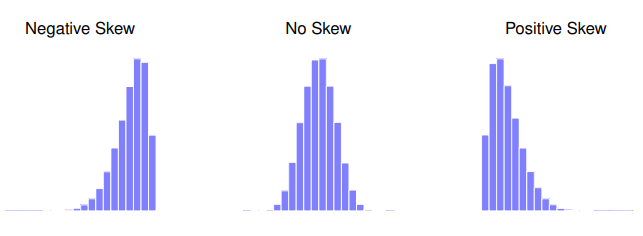
\includegraphics{./images/fig4-11.png} \hfill{}

\caption{\label{fig-fig4-11}An illustration of skewness. On the left we
have a negatively skewed data set, in the middle we have a data set with
no skew, and on the right we have a positively skewed data set}

\end{figure}

Since it's the more interesting of the two, let's start by talking about
the \textbf{skewness}. Skewness is basically a measure of asymmetry and
the easiest way to explain it is by drawing some pictures. As
Figure~\ref{fig-fig4-11} illustrates, if the data tend to have a lot of
extreme small values (i.e., the lower tail is ``longer'' than the upper
tail) and not so many extremely large values (left panel) then we say
that the data are \emph{negatively skewed}. On the other hand, if there
are more extremely large values than extremely small ones (right panel)
we say that the data are positively skewed. That's the qualitative idea
behind skewness. If there are relatively more values that are far
greater than the mean, the distribution is positively skewed or right
skewed, with a tail stretching to the right. Negative or left skew is
the opposite. A symmetric distribution has a skewness of 0. The skewness
value for a positively skewed distribution is positive, and a negative
value for a negatively skewed distribution.

{[}Additional technical detail\footnote{One formula for the skewness of
  a data set is as follows
  \[skewness(X)=\frac{1}{N \hat{\sigma}^3} \sum_{i=1}^{N} ( X_i - \bar{X})^3\]
  where N is the number of observations, \(\bar{X}\) is the sample mean,
  and \(\hat{\sigma}\) is the standard deviation (the ``divide by
  \(N - 1\)'' version, that is).}{]}

Perhaps more helpfully, you can use jamovi to calculate skewness: it's a
check box in the `Statistics' options under `Exploration' -
`Descriptives'. For the afl.margins variable, the skewness figure is
\(0.780\). If you divide the skewness estimate by the Std. error for
skewness you have an indication of how skewed the data is. Especially in
small samples (N \(<\) 50), one rule of thumb suggests that a value of 2
or less can mean that the data is not very skewed, and a value of over 2
that there is sufficient skew in the data to possibly limit its use in
some statistical analyses. Though there is no clear agreement on this
interpretation. That said, this does indicate that the AFL winning
margins data is somewhat skewed (\(\frac{0.780}{0.183} = 4.262\)).

The final measure that is sometimes referred to, though very rarely in
practice, is the kurtosis of a data set. Put simply, kurtosis is a
measure of how thin or fat the tails of a distribution are, as
illustrated in Figure~\ref{fig-fig4-12}. By convention, we say that the
``normal curve'' (black lines) has zero kurtosis, so the degree of
kurtosis is assessed relative to this curve.

\begin{figure}

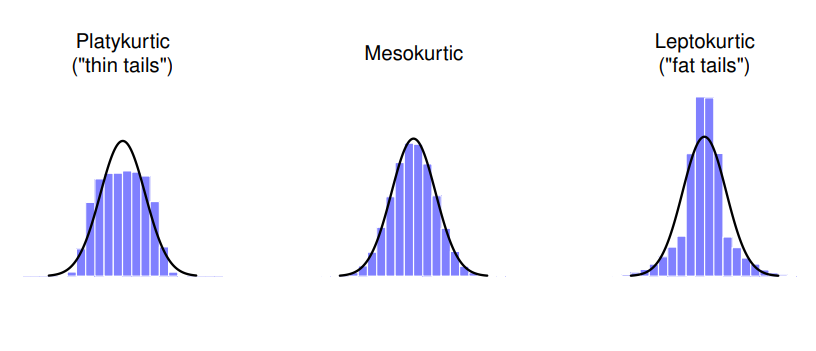
\includegraphics{./images/fig4-12.png} \hfill{}

\caption{\label{fig-fig4-12}An illustration of kurtosis. On the left, we
have a `platykurtic' distribution (kurtosis = -.95) meaning that the
distribution has `thin' or flat tails. In the middle we have a
`mesokurtic' distribution (kurtosis is almost exactly 0) which means
that the tails are neither thin or fat. Finally, on the right, we have a
`leptokurtic' distribution (kurtosis = 2.12) indicating that the
distribution has `fat' tails. Note that kurtosis is measured with
respect to a normal curve (black line)}

\end{figure}

In this Figure, the data on the left have a pretty flat distribution,
with thin tails, so the kurtosis is negative and we call the data
platykurtic. The data on the right have a distribution with fat tails,
so the kurtosis is positive and we say that the data is leptokurtic. But
the data in the middle have neither think or fat tails, so we say that
it is mesokurtic and has kurtosis zero. This is summarised in
Table~\ref{tbl-tab4-4}:

\hypertarget{tbl-tab4-4}{}
 
  \providecommand{\huxb}[2]{\arrayrulecolor[RGB]{#1}\global\arrayrulewidth=#2pt}
  \providecommand{\huxvb}[2]{\color[RGB]{#1}\vrule width #2pt}
  \providecommand{\huxtpad}[1]{\rule{0pt}{#1}}
  \providecommand{\huxbpad}[1]{\rule[-#1]{0pt}{#1}}

\begin{table}[ht]
\caption{\label{tbl-tab4-4}Thin to fat tails to illustrate kurtosis }\tabularnewline

\begin{centerbox}
\begin{threeparttable}
\setlength{\tabcolsep}{0pt}
\begin{tabularx}{0.9\textwidth}{p{0.3\textwidth} p{0.3\textwidth} p{0.3\textwidth}}


\hhline{>{\huxb{0, 0, 0}{0.4}}->{\huxb{0, 0, 0}{0.4}}->{\huxb{0, 0, 0}{0.4}}-}
\arrayrulecolor{black}

\multicolumn{1}{!{\huxvb{0, 0, 0}{0}}p{0.3\textwidth}!{\huxvb{0, 0, 0}{0}}}{\cellcolor[RGB]{242, 242, 242}\hspace{0pt}\parbox[b]{0.3\textwidth-0pt-6pt}{\huxtpad{6pt + 1em}\centering \textbf{English}\huxbpad{6pt}}} &
\multicolumn{1}{p{0.3\textwidth}!{\huxvb{0, 0, 0}{0}}}{\cellcolor[RGB]{242, 242, 242}\hspace{6pt}\parbox[b]{0.3\textwidth-6pt-6pt}{\huxtpad{6pt + 1em}\centering \textbf{informal term}\huxbpad{6pt}}} &
\multicolumn{1}{p{0.3\textwidth}!{\huxvb{0, 0, 0}{0}}}{\cellcolor[RGB]{242, 242, 242}\hspace{6pt}\parbox[b]{0.3\textwidth-6pt-0pt}{\huxtpad{6pt + 1em}\centering \textbf{kurtosis value}\huxbpad{6pt}}} \tabularnewline[-0.5pt]


\hhline{>{\huxb{0, 0, 0}{0.4}}->{\huxb{0, 0, 0}{0.4}}->{\huxb{0, 0, 0}{0.4}}-}
\arrayrulecolor{black}

\multicolumn{1}{!{\huxvb{0, 0, 0}{0}}p{0.3\textwidth}!{\huxvb{0, 0, 0}{0}}}{\hspace{0pt}\parbox[b]{0.3\textwidth-0pt-6pt}{\huxtpad{6pt + 1em}\centering "tails too thin"\huxbpad{6pt}}} &
\multicolumn{1}{p{0.3\textwidth}!{\huxvb{0, 0, 0}{0}}}{\hspace{6pt}\parbox[b]{0.3\textwidth-6pt-6pt}{\huxtpad{6pt + 1em}\centering platykurtic\huxbpad{6pt}}} &
\multicolumn{1}{p{0.3\textwidth}!{\huxvb{0, 0, 0}{0}}}{\hspace{6pt}\parbox[b]{0.3\textwidth-6pt-0pt}{\huxtpad{6pt + 1em}\centering negative\huxbpad{6pt}}} \tabularnewline[-0.5pt]


\hhline{}
\arrayrulecolor{black}

\multicolumn{1}{!{\huxvb{0, 0, 0}{0}}p{0.3\textwidth}!{\huxvb{0, 0, 0}{0}}}{\cellcolor[RGB]{242, 242, 242}\hspace{0pt}\parbox[b]{0.3\textwidth-0pt-6pt}{\huxtpad{6pt + 1em}\centering "tails neither thin or fat"\huxbpad{6pt}}} &
\multicolumn{1}{p{0.3\textwidth}!{\huxvb{0, 0, 0}{0}}}{\cellcolor[RGB]{242, 242, 242}\hspace{6pt}\parbox[b]{0.3\textwidth-6pt-6pt}{\huxtpad{6pt + 1em}\centering mesokurtic\huxbpad{6pt}}} &
\multicolumn{1}{p{0.3\textwidth}!{\huxvb{0, 0, 0}{0}}}{\cellcolor[RGB]{242, 242, 242}\hspace{6pt}\parbox[b]{0.3\textwidth-6pt-0pt}{\huxtpad{6pt + 1em}\centering zero\huxbpad{6pt}}} \tabularnewline[-0.5pt]


\hhline{}
\arrayrulecolor{black}

\multicolumn{1}{!{\huxvb{0, 0, 0}{0}}p{0.3\textwidth}!{\huxvb{0, 0, 0}{0}}}{\hspace{0pt}\parbox[b]{0.3\textwidth-0pt-6pt}{\huxtpad{6pt + 1em}\centering "tails too fat"\huxbpad{6pt}}} &
\multicolumn{1}{p{0.3\textwidth}!{\huxvb{0, 0, 0}{0}}}{\hspace{6pt}\parbox[b]{0.3\textwidth-6pt-6pt}{\huxtpad{6pt + 1em}\centering leptokurtic\huxbpad{6pt}}} &
\multicolumn{1}{p{0.3\textwidth}!{\huxvb{0, 0, 0}{0}}}{\hspace{6pt}\parbox[b]{0.3\textwidth-6pt-0pt}{\huxtpad{6pt + 1em}\centering positive\huxbpad{6pt}}} \tabularnewline[-0.5pt]


\hhline{>{\huxb{0, 0, 0}{0.4}}->{\huxb{0, 0, 0}{0.4}}->{\huxb{0, 0, 0}{0.4}}-}
\arrayrulecolor{black}
\end{tabularx} 

\end{threeparttable}\par\end{centerbox}

\end{table}
 

{[}Additional technical detail\footnote{The equation for kurtosis is
  pretty similar in spirit to the formulas we've seen already for the
  variance and the skewness. Except that where the variance involved
  squared deviations and the skewness involved cubed deviations, the
  kurtosis involves raising the deviations to the fourth power:\(^b\)
  \[kurtosis(X)=\frac{1}{N \hat{\sigma}^4} \sum_{i=1}^{N} ( X_i - \bar{X} )^4 - 3\]
  I know, it's not terribly interesting to me either. --- \(^b\) The
  ``-3'' part is something that statisticians tack on to ensure that the
  normal curve has kurtosis zero. It looks a bit stupid, just sticking a
  ``-3'' at the end of the formula, but there are good mathematical
  reasons for doing this.}{]}

More to the point, jamovi has a check box for kurtosis just below the
check box for skewness, and this gives a value for kurtosis of \(0.101\)
with a standard error of \(0.364\). This means that the AFL winning
margins data has only a small kurtosis, which is ok.

\hypertarget{descriptive-statistics-separately-for-each-group}{%
\section{Descriptive statistics separately for each
group}\label{descriptive-statistics-separately-for-each-group}}

It is very commonly the case that you find yourself needing to look at
descriptive statistics broken down by some grouping variable. This is
pretty easy to do in jamovi. For instance, let's say I want to look at
the descriptive statistics for some clinical trial data, broken down
separately by therapy type. This is a new data set, one that you've
never seen before. The data is stored in the clinicaltrial.csv file and
we'll use it a lot later on in
Chapter~\ref{sec-Comparing-several-means-one-way-ANOVA} (you can find a
complete description of the data at the start of that chapter). Let's
load it and see what we've got (Figure~\ref{fig-fig4-13}):

Evidently there were three drugs: a placebo, something called
``anxifree'' and something called ``joyzepam'', and there were 6 people
administered each drug. There were 9 people treated using cognitive
behavioural therapy (CBT) and 9 people who received no psychological
treatment. And we can see from looking at the `Descriptives' of the
mood.gain variable that most people did show a mood gain
(\(mean = 0.88\)), though without knowing what the scale is here it's
hard to say much more than that. Still, that's not too bad. Overall I
feel that I learned something from that.

We can also go ahead and look at some other descriptive statistics, and
this time separately for each type of therapy. In jamovi, check Std.
deviation, Skewness and Kurtosis in the `Statistics' options. At the
same time, transfer the therapy variable into the `Split by' box, and
you should get something like Figure~\ref{fig-fig4-14}.

\begin{figure}

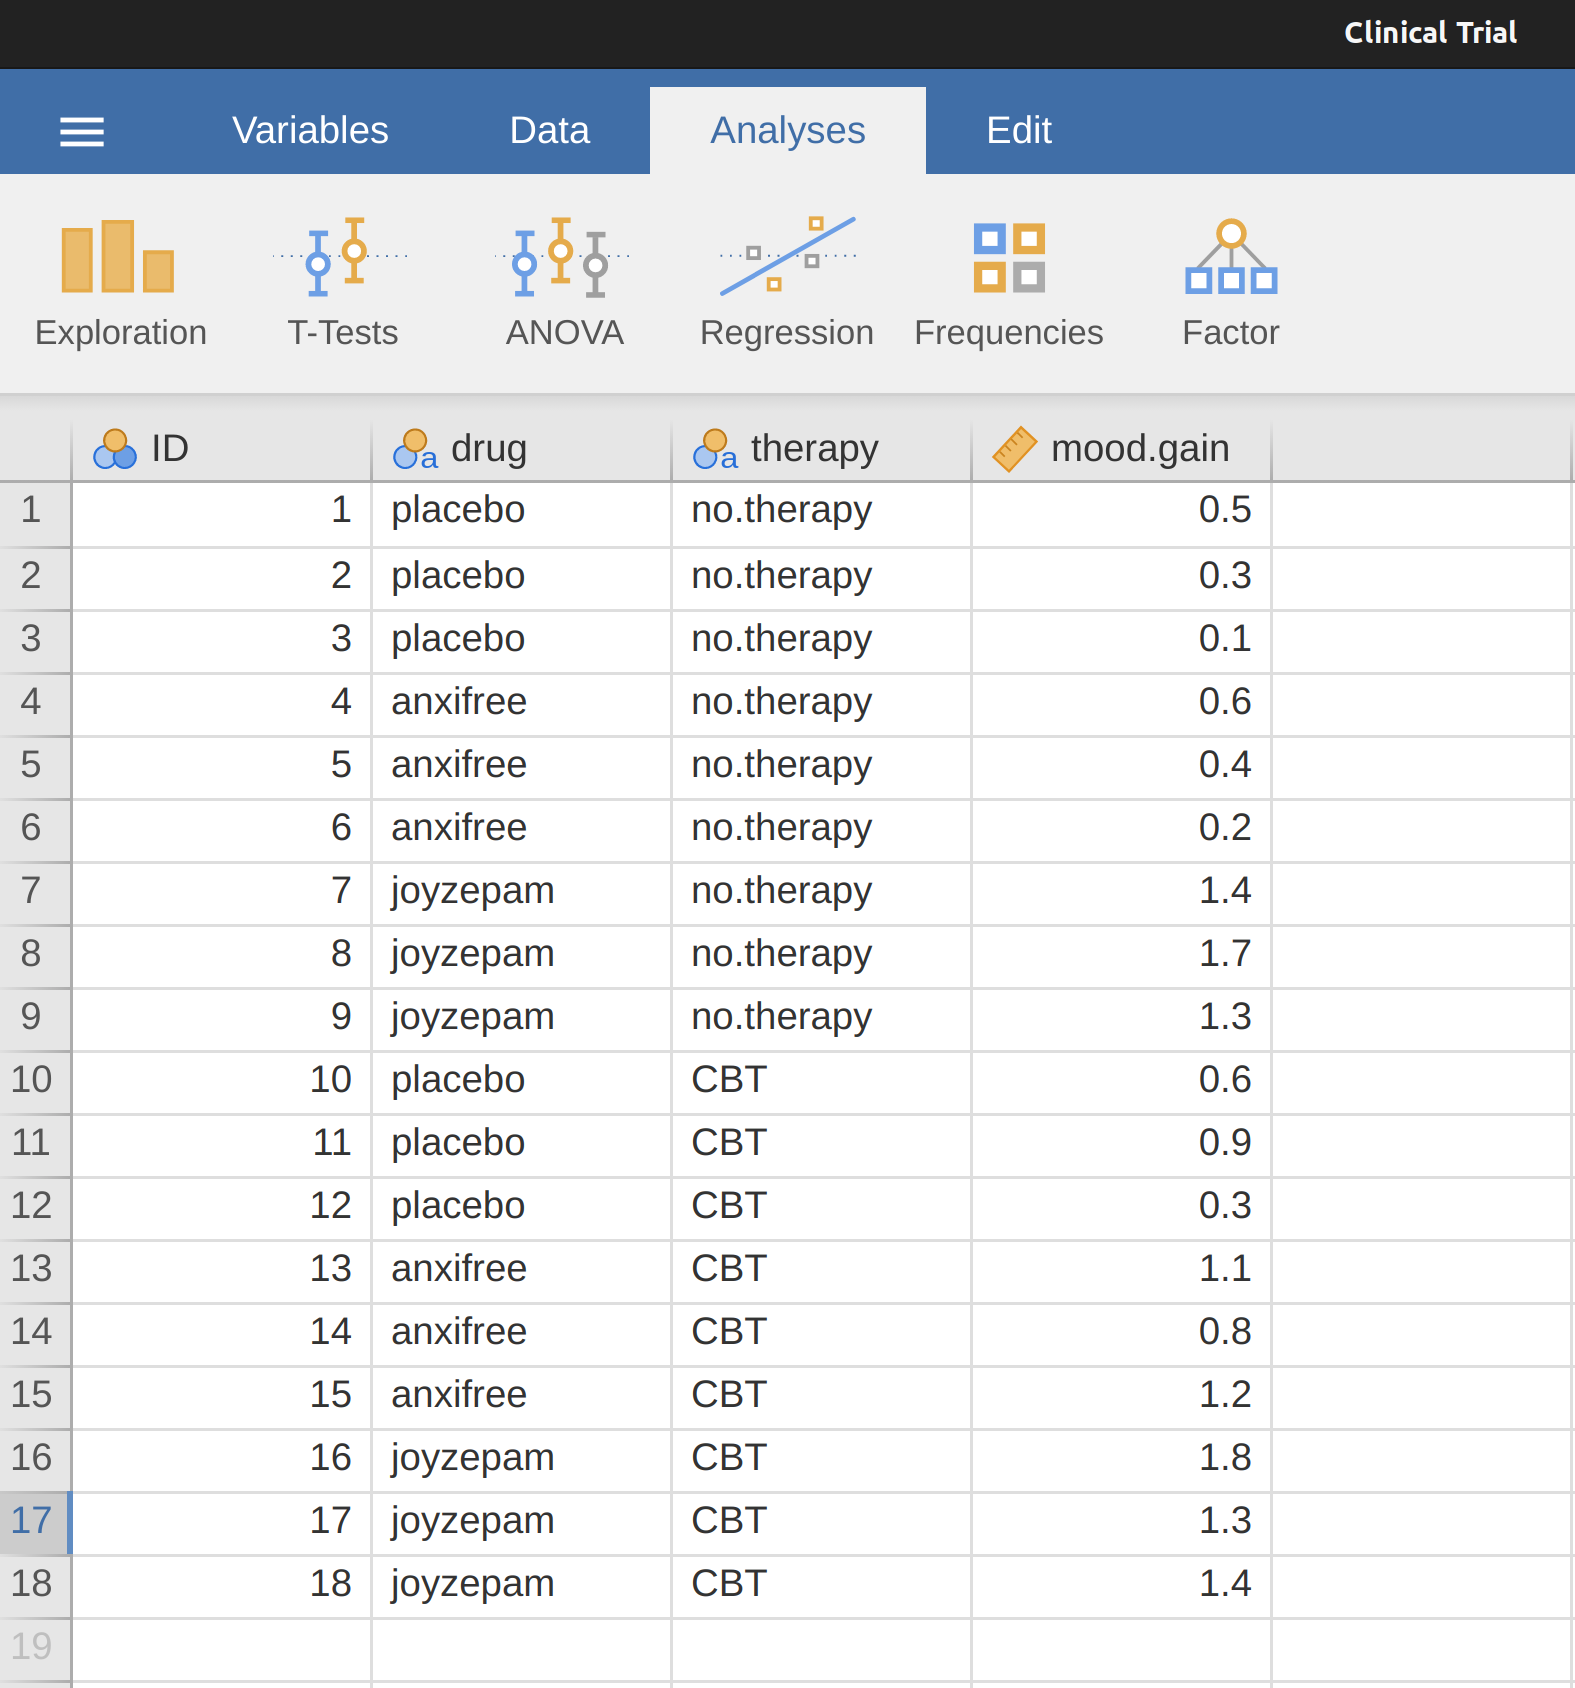
\includegraphics{./images/fig4-13.png} \hfill{}

\caption{\label{fig-fig4-13}A screenshot of jamovi showing the variables
stored in the clinicaltrial.csv file}

\end{figure}

What if you have multiple grouping variables? Suppose you want to look
at the average mood gain separately for all possible combinations of
drug and therapy. It is possible to do this by adding another variable,
drug, into the `Split by' box. Easy peasy, though sometimes if you split
too much there isn't enough data in each breakdown combination to make
meaningful calculations. In this case jamovi tells you this by stating
something like NaN or Inf. \footnote{Sometimes jamovi will also present
  numbers in an unusual way. If a number is very small, or very large,
  then jamovi switches to an exponential form for numbers. For example
  6.51e-4 is the same as saying that the decimal point is moved 4 places
  to the left, so the actual number is 0.000651. If there is a plus sign
  (i.e.~6.51e+4 then the decimal point is moved to the right,
  i.e.~65,100.00. Usually only very small or very large numbers are
  expressed in this way, for example 6.51e-16, which would be quite
  unwieldy to write out in the normal way.}

\begin{figure}

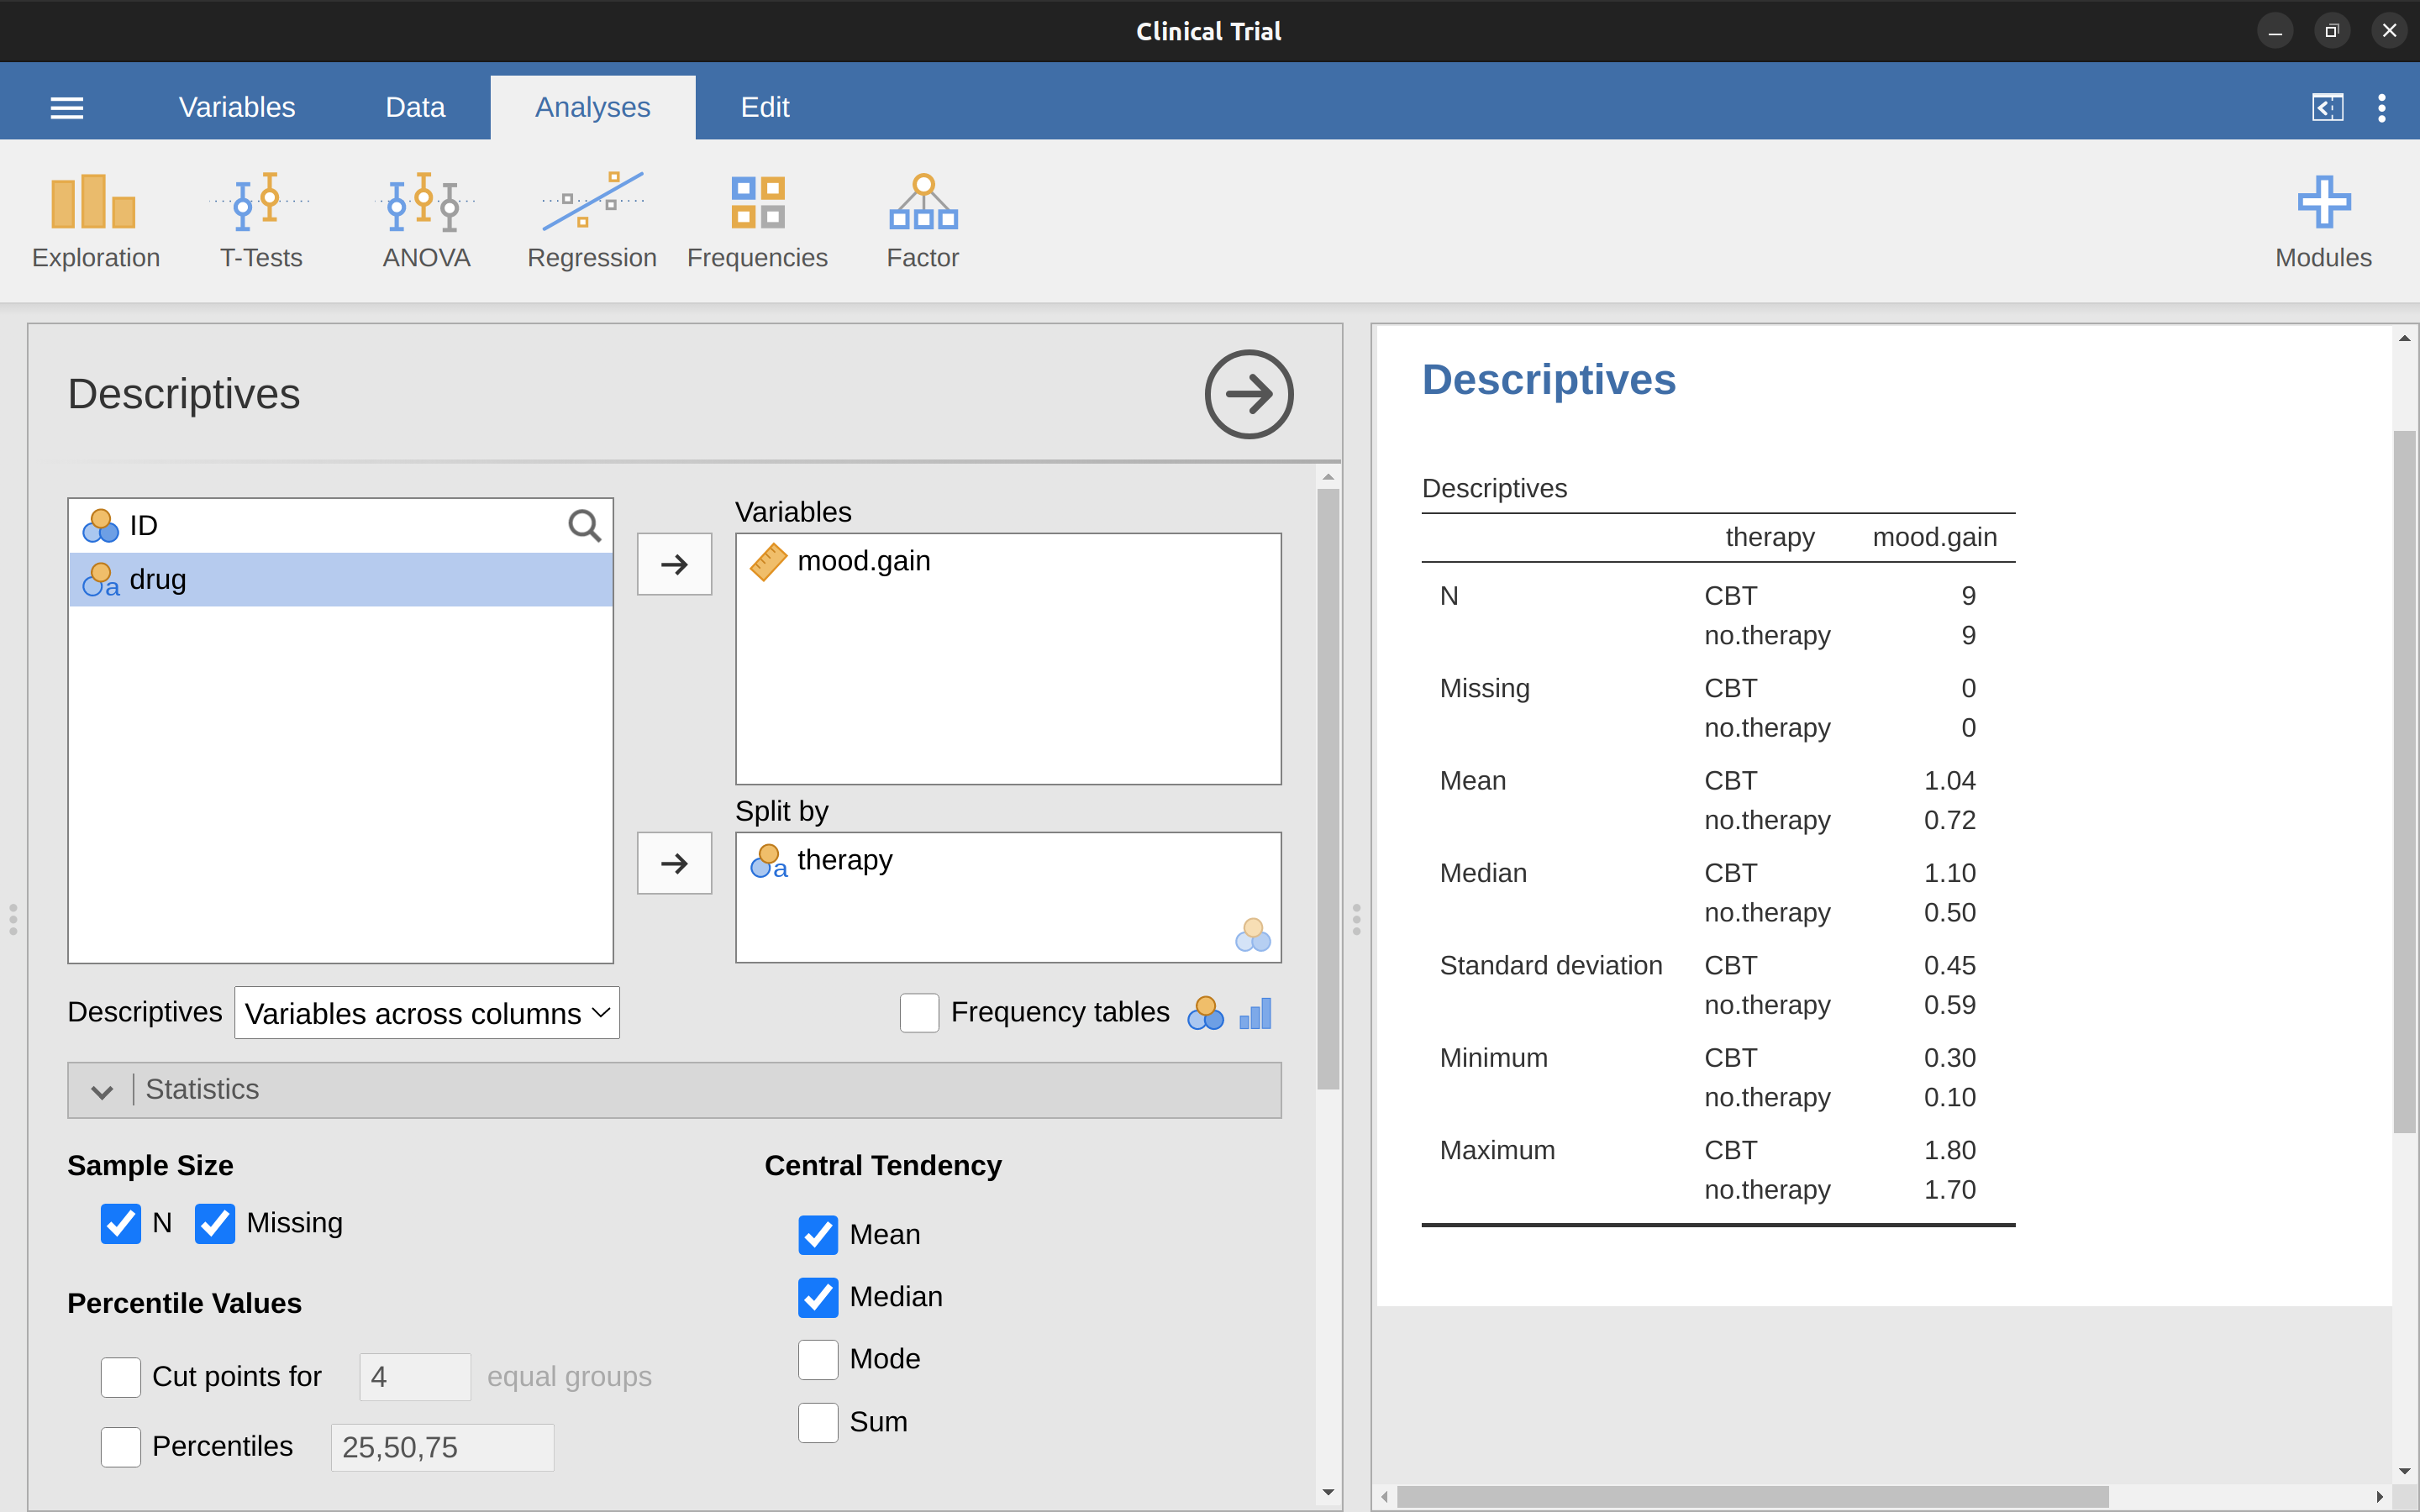
\includegraphics{./images/fig4-14.png} \hfill{}

\caption{\label{fig-fig4-14}A screenshot of jamovi showing Descriptives
split by therapy type}

\end{figure}

\hypertarget{sec-Standard-scores}{%
\section{Standard scores}\label{sec-Standard-scores}}

Suppose my friend is putting together a new questionnaire intended to
measure ``grumpiness''. The survey has \(50\) questions which you can
answer in a grumpy way or not. Across a big sample (hypothetically,
let's imagine a million people or so!) the data are fairly normally
distributed, with the mean grumpiness score being \(17\) out of \(50\)
questions answered in a grumpy way, and the standard deviation is \(5\).
In contrast, when I take the questionnaire I answer \(35\) out of \(50\)
questions in a grumpy way. So, how grumpy am I? One way to think about
it would be to say that I have grumpiness of \(\frac{35}{50}\), so you
might say that I'm 70\% grumpy. But that's a bit weird, when you think
about it. If my friend had phrased her questions a bit differently
people might have answered them in a different way, so the overall
distribution of answers could easily move up or down depending on the
precise way in which the questions were asked. So, I'm only 70\% grumpy
\emph{with respect to this set of survey questions}. Even if it's a very
good questionnaire this isn't very a informative statement.

A simpler way around this is to describe my grumpiness by comparing me
to other people. Shockingly, out of my friend's sample of \(1,000,000\)
people, only \(159\) people were as grumpy as me (that's not at all
unrealistic, frankly) suggesting that I'm in the top 0.016\% of people
for grumpiness. This makes much more sense than trying to interpret the
raw data. This idea, that we should describe my grumpiness in terms of
the overall distribution of the grumpiness of humans, is the qualitative
idea that standardisation attempts to get at. One way to do this is to
do exactly what I just did and describe everything in terms of
percentiles. However, the problem with doing this is that ``it's lonely
at the top''. Suppose that my friend had only collected a sample of
\(1000\) people (still a pretty big sample for the purposes of testing a
new questionnaire, I'd like to add), and this time gotten, let's say, a
mean of \(16\) out of \(50\) with a standard deviation of \(5\). The
problem is that almost certainly not a single person in that sample
would be as grumpy as me.

However, all is not lost. A different approach is to convert my
grumpiness score into a \textbf{standard score}, also referred to as a
z-score. The standard score is defined as the number of standard
deviations above the mean that my grumpiness score lies. To phrase it in
``pseudomaths'' the standard score is calculated like this:

\[
\text{standard score} = \frac{\text{raw score} - mean}{\text{standard deviation}}
\]

{[}Additional technical detail\footnote{In actual maths, the equation
  for the z-score is \[z_i =\frac{X_i - \bar{X}}{\hat{\sigma}}\]}{]}

So, going back to the grumpiness data, we can now transform Dani's raw
grumpiness into a standardised grumpiness score.

\[ z =\frac{35 - 17}{5} = 3.6 \] To interpret this value, recall the
rough heuristic that I provided in Section~\ref{sec-Standard-deviation}
in which I noted that 99.7\% of values are expected to lie within 3
standard deviations of the mean. So the fact that my grumpiness
corresponds to a z score of 3.6 indicates that I'm very grumpy indeed.
In fact this suggests that I'm grumpier than 99.98\% of people. Sounds
about right.

In addition to allowing you to interpret a raw score in relation to a
larger population (and thereby allowing you to make sense of variables
that lie on arbitrary scales), standard scores serve a second useful
function. Standard scores can be compared to one another in situations
where the raw scores can't. Suppose, for instance, my friend also had
another questionnaire that measured extraversion using a \(24\) item
questionnaire. The overall mean for this measure turns out to be 13 with
standard deviation \(4\), and I scored a \(2\). As you can imagine, it
doesn't make a lot of sense to try to compare my raw score of \(2\) on
the extraversion questionnaire to my raw score of 35 on the grumpiness
questionnaire. The raw scores for the two variables are ``about''
fundamentally different things, so this would be like comparing apples
to oranges.

What about the standard scores? Well, this is a little different. If we
calculate the standard scores we get \((z = \frac{(35-17)}{5}=3.6)\) for
grumpiness and \((z = \frac{(2-13)}{4}=-2.75)\) for extraversion. These
two numbers can be compared to each other.\footnote{Though some caution
  is usually warranted. It's not always the case that one standard
  deviation on variable A corresponds to the same ``kind'' of thing as
  one standard deviation on variable B. Use common sense when trying to
  determine whether or not the z scores of two variables can be
  meaningfully compared} I'm much less extraverted than most people
(\(z = -2.75\)) and much grumpier than most people (\(z=3.6\)). But the
extent of my unusualness is much more extreme for grumpiness, since
\(3.6\) is a bigger number than \(2.75\). Because each standardised
score is a statement about where an observation falls relative to its
own population, it is possible to compare standardised scores across
completely different variables.

\hypertarget{summary-2}{%
\section{Summary}\label{summary-2}}

Calculating some basic descriptive statistics is one of the very first
things you do when analysing real data, and descriptive statistics are
much simpler to understand than inferential statistics, so like every
other statistics textbook I've started with descriptives. In this
chapter, we talked about the following topics:

\begin{itemize}
\tightlist
\item
  \protect\hyperlink{measures-of-central-tendency}{Measures of central
  tendency}. Broadly speaking, central tendency measures tell you where
  the data are. There's three measures that are typically reported in
  the literature: the mean, median and mode.
\item
  \protect\hyperlink{sec-Measures-of-variability}{Measures of
  variability}. In contrast, measures of variability tell you about how
  ``spread out'' the data are. The key measures are: range, standard
  deviation, and interquartile range.
\item
  \protect\hyperlink{skew-and-kurtosis}{Skew and kurtosis}. We also
  looked at assymetry in a variable's distribution (skew) and thin or
  fat tailed distributions (kurtosis).
\item
  \protect\hyperlink{descriptive-statistics-separately-for-each-group}{Descriptive
  statistics separately for each group}. Since this book focuses on
  doing data analysis in jamovi, we spent a bit of time talking about
  how descriptive statistics are computed for different subgroups.
\item
  \protect\hyperlink{sec-Standard-scores}{Standard scores}. The z-score
  is a slightly unusual beast. It's not quite a descriptive statistic,
  and not quite an inference. Make sure you understand this section.
  It'll come up again later.
\end{itemize}

In the next Chapter we'll move on to a discussion of how to draw
pictures! Everyone loves a pretty picture, right? But before we do, I
want to end on an important point. A traditional first course in
statistics spends only a small proportion of the class on descriptive
statistics, maybe one or two lectures at most. The vast majority of the
lecturer's time is spent on inferential statistics because that's where
all the hard stuff is. That makes sense, but it hides the practical
everyday importance of choosing good descriptives. With that in
mind\ldots{}

\hypertarget{sec-Drawing-graphs}{%
\chapter{Drawing graphs}\label{sec-Drawing-graphs}}

\begin{quote}
\emph{Above all else show the data.}\\
-- Edward Tufte\footnote{The origin of this quote is Tufte's lovely book
  \emph{The Visual Display of Quantitative Information.}}
\end{quote}

Visualising data is one of the most important tasks facing the data
analyst. It's important for two distinct but closely related reasons.
Firstly, there's the matter of drawing ``presentation graphics'',
displaying your data in a clean, visually appealing fashion makes it
easier for your reader to understand what you're trying to tell them.
Equally important, perhaps even more important, is the fact that drawing
graphs helps you to understand the data. To that end, it's important to
draw ``exploratory graphics'' that help you learn about the data as you
go about analysing it. These points might seem pretty obvious but I
cannot count the number of times I've seen people forget them.

To give a sense of the importance of this chapter, I want to start with
a classic illustration of just how powerful a good graph can be. To that
end, Figure~\ref{fig-fig5-1} shows a redrawing of one of the most famous
data visualisations of all time. This is John Snow's 1854 map of cholera
deaths. The map is elegant in its simplicity. In the background we have
a street map which helps orient the viewer. Over the top we see a large
number of small dots, each one representing the location of a cholera
case. The larger symbols show the location of water pumps, labelled by
name. Even the most casual inspection of the graph makes it very clear
that the source of the outbreak is almost certainly the Broad Street
pump. Upon viewing this graph Dr Snow arranged to have the handle
removed from the pump and ended the outbreak that had killed over 500
people. Such is the power of a good data visualisation.

The goals in this chapter are twofold. First, to discuss several fairly
standard graphs that we use a lot when analysing and presenting data,
and second to show you how to create these graphs in jamovi. The graphs
themselves tend to be pretty straightforward, so in one respect this
chapter is pretty simple. Where people usually struggle is learning how
to produce graphs, and especially learning how to produce good graphs.
Fortunately, learning how to draw graphs in jamovi is reasonably simple
as long as you're not too picky about what your graph looks like. What I
mean when I say this is that jamovi has a lot of very good default
graphs, or plots, that most of the time produce a clean, high-quality
graphic. However, on those occasions when you do want to do something
non-standard, or if you need to make highly specific changes to the
figure, then the graphics functionality in jamovi is not yet capable of
supporting advanced work or detail editing.

\begin{figure}

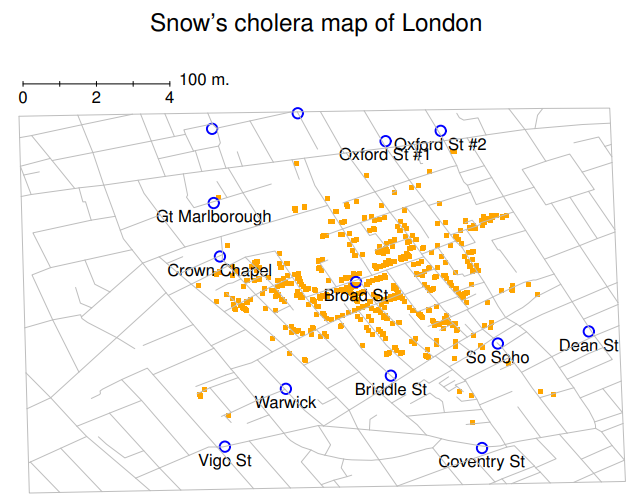
\includegraphics{./images/fig5-1.png} \hfill{}

\caption{\label{fig-fig5-1}A stylised redrawing of John Snow's original
cholera map. Each small dot represents the location of a cholera case
and each large circle shows the location of a well. As the plot makes
clear, the cholera outbreak is centred very closely on the Broad St
pump}

\end{figure}

\hypertarget{sec-Histograms}{%
\section{Histograms}\label{sec-Histograms}}

Let's begin with the humble \textbf{histogram}. Histograms are one of
the simplest and most useful ways of visualising data. They make most
sense when you have an interval or ratio scale variable (e.g., the
afl.margins data from Chapter~\ref{sec-Descriptive-statistics} and what
you want to do is get an overall impression of the variable. Most of you
probably know how histograms work, since they're so widely used, but for
the sake of completeness I'll describe them. All you do is divide up the
possible values into \textbf{bins} and then count the number of
observations that fall within each bin. This count is referred to as the
frequency or density of the bin and is displayed as a vertical bar. Ihe
AFL winning margins data there are 33 games in which the winning margin
was less than 10 points and it is this fact that is represented by the
height of the leftmost bar that we showed earlier in
Chapter~\ref{sec-Descriptive-statistics}, Figure~\ref{fig-fig4-2}. With
these earlier graphs we used an advanced plotting package in R which,
for now, is beyond the capability of jamovi. But jamovi gets us close,
and drawing this histogram in jamovi is pretty straightforward. Open up
the `plots' options under `Exploration' - `Descriptives' and click the
`histogram' check box, as in Figure~\ref{fig-fig5-1}. jamovi defaults to
labelling the y-axis as `density' and the x-axis with the variable name.
The \textbf{bins} are selected automatically, and there is no scale, or
count, information on the y-axis unlike the previous
Figure~\ref{fig-fig4-2}. But this does not matter too much because after
all what we are really interested in is our impression of the shape of
the distribution: is it normally distributed or is there a skew or
kurtosis? Our first impressions of these characteristics come from
drawing a \textbf{histogram}.

\begin{figure}

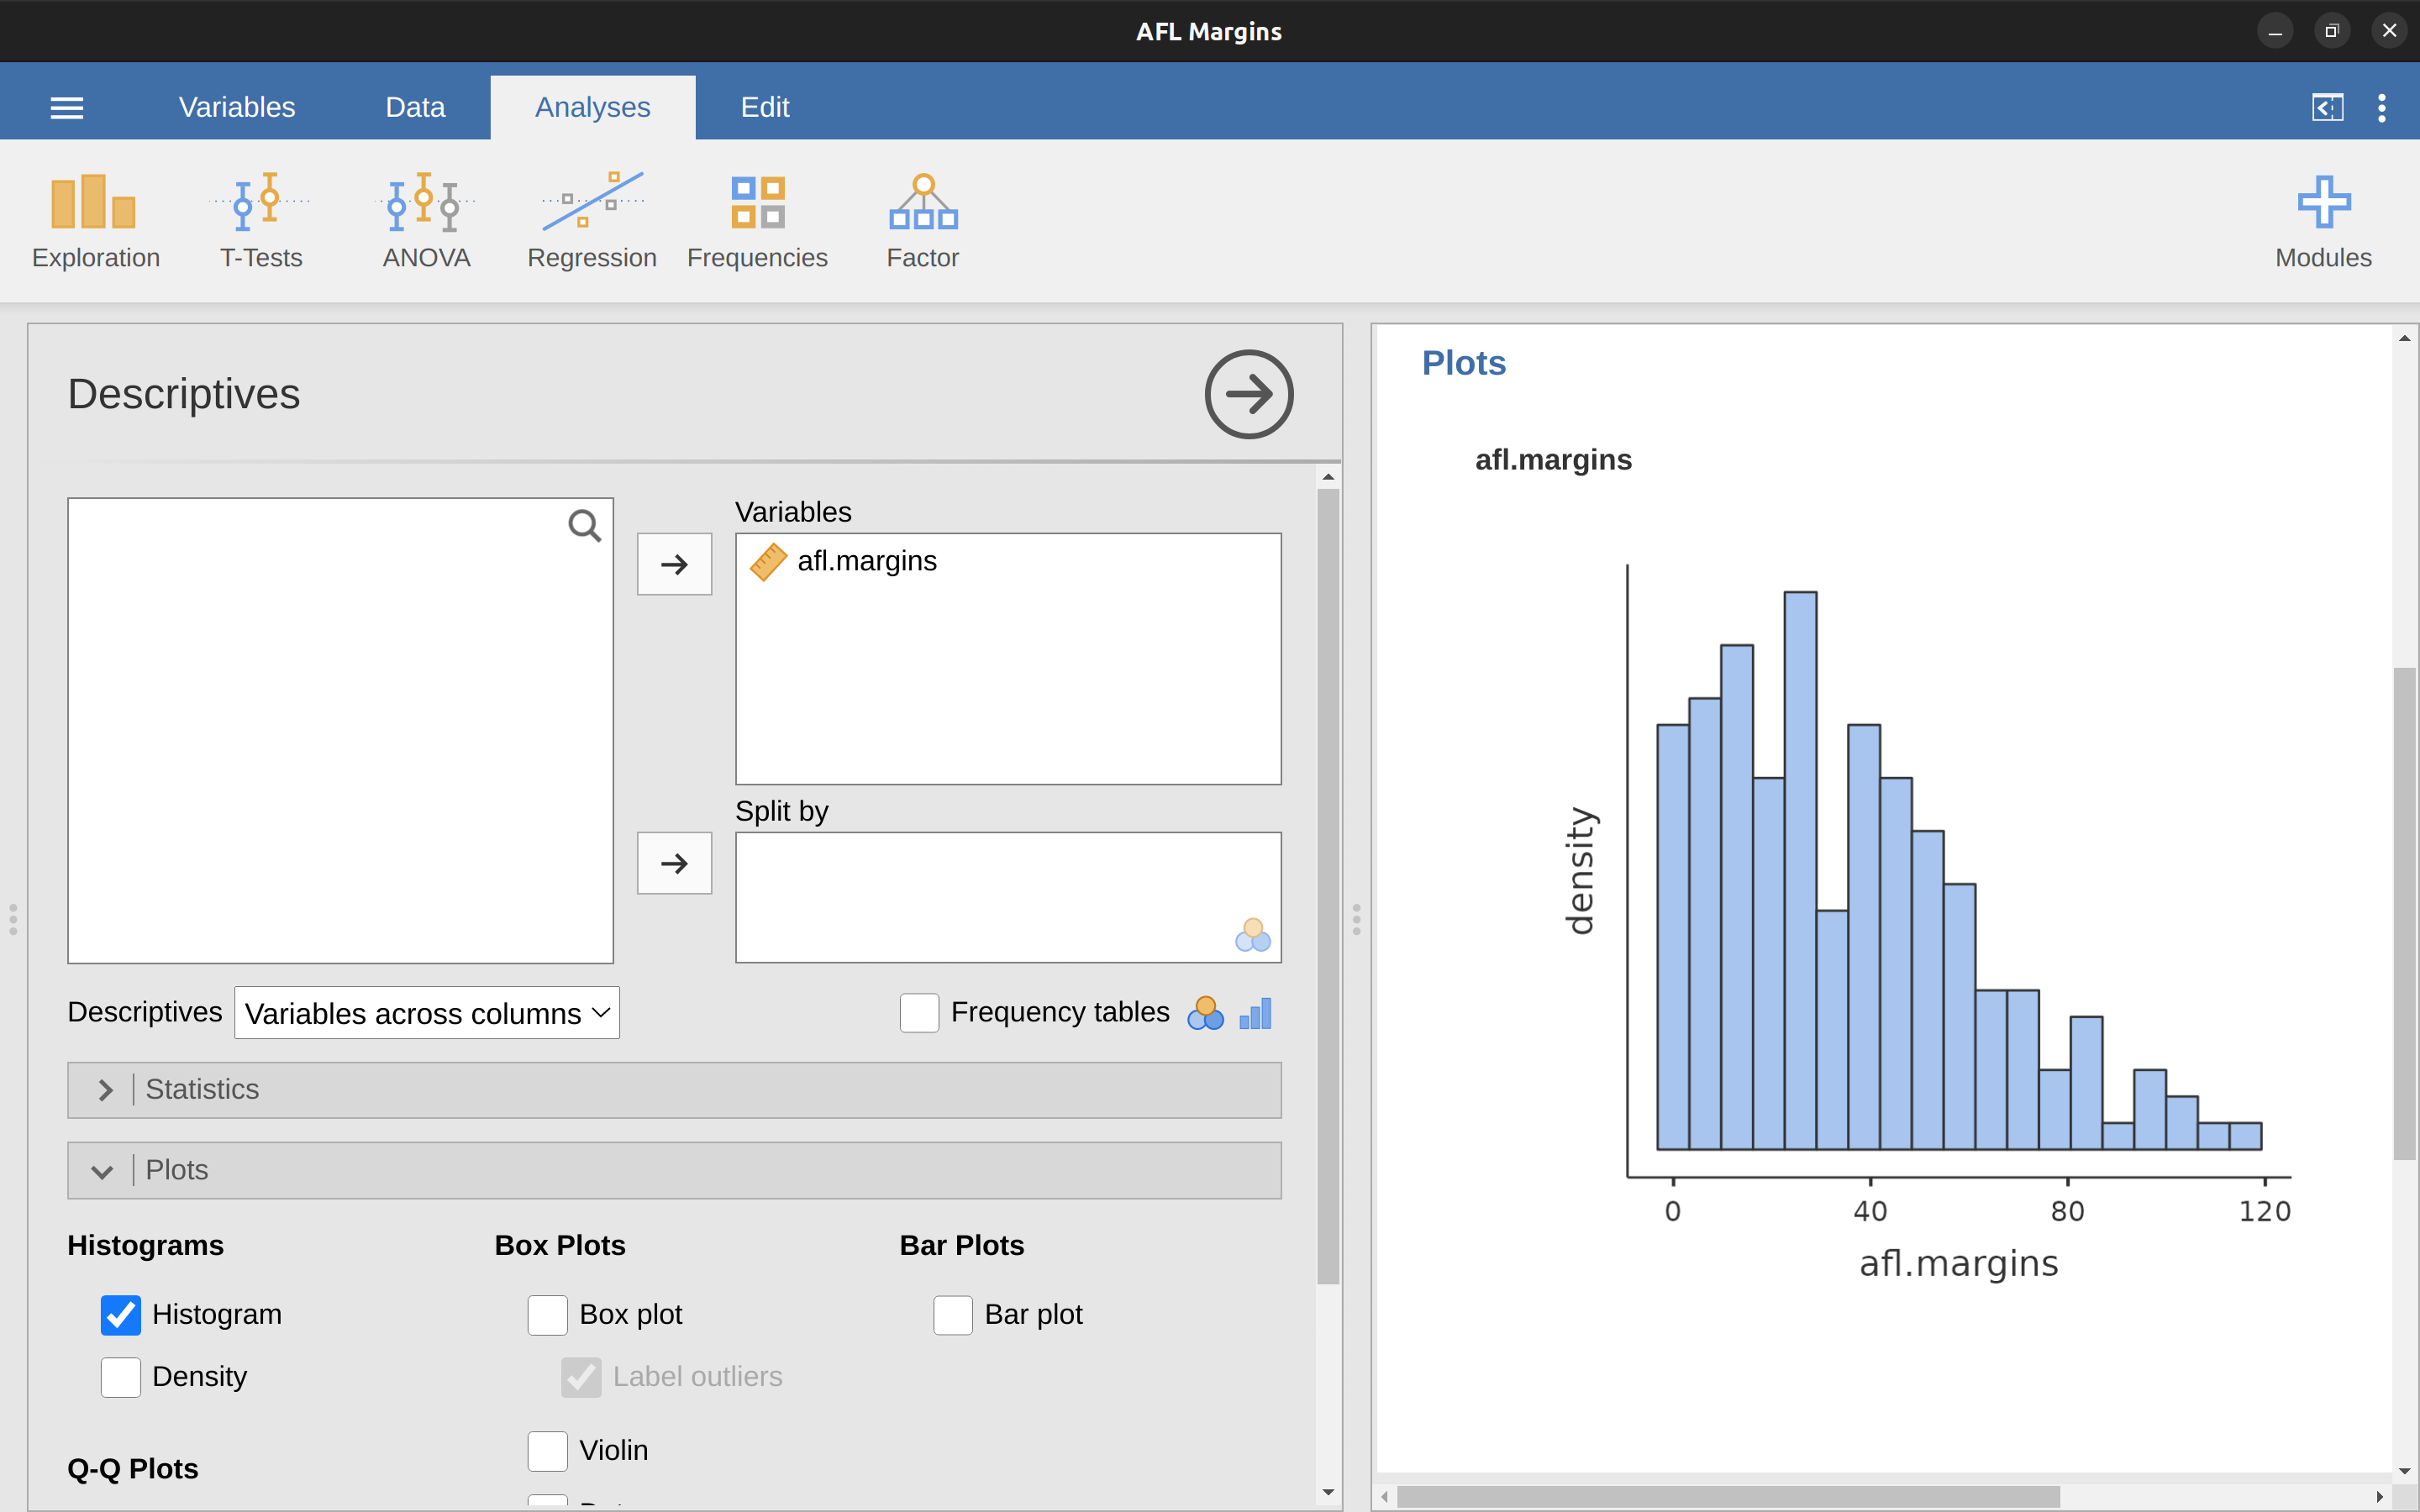
\includegraphics{./images/fig5-2.png} \hfill{}

\caption{\label{fig-fig5-2}jamovi screen showing the histogram check
box}

\end{figure}

One additional feature that jamovi provides is the ability to plot a
`Density' curve. You can do this by clicking the `Density' check box
under the `Plots' options (and unchecking `Histogram'), and this gives
us the plot shown in Figure~\ref{fig-fig5-3}. A density plot visualises
the distribution of data over a continuous interval or time period. This
chart is a variation of a histogram that uses \textbf{kernel smoothing}
to plot values, allowing for smoother distributions by smoothing out the
noise. The peaks of a density plot help display where values are
concentrated over the interval. An advantage density plots have over
histograms is that they are better at determining the distribution shape
because they're not affected by the number of bins used (each bar used
in a typical histogram). A histogram comprising of only 4 bins wouldn't
produce a distinguishable enough shape of distribution as a 20-bin
histogram would. However, with density plots, this isn't an issue.

\begin{figure}

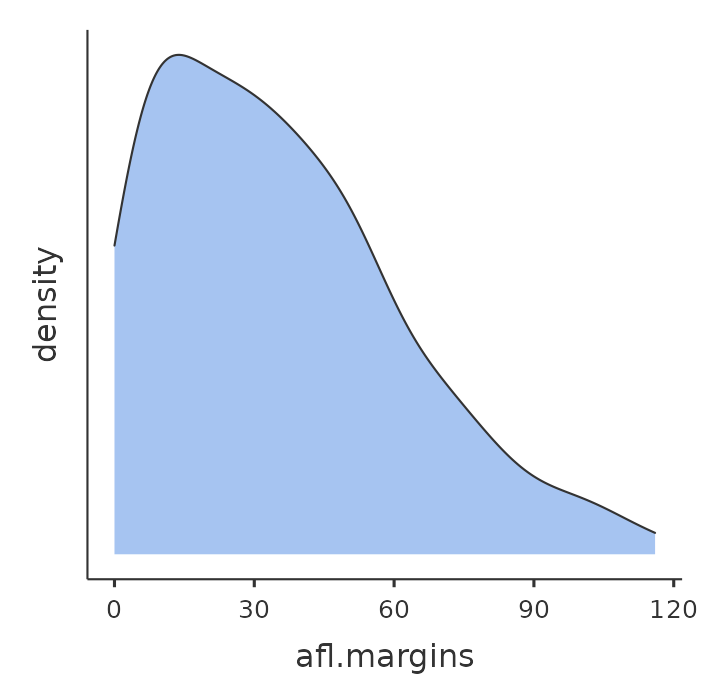
\includegraphics{./images/fig5-3.png} \hfill{}

\caption{\label{fig-fig5-3}A density plot of the afl.margins variable
plotted in jamovi}

\end{figure}

Although this image would need a lot of cleaning up in order to make a
good presentation graphic (i.e., one you'd include in a report), it
nevertheless does a pretty good job of describing the data. In fact, the
big strength of a histogram or density plot is that (properly used) it
does show the entire spread of the data, so you can get a pretty good
sense about what it looks like. The downside to histograms is that they
aren't very compact. Unlike some of the other plots I'll talk about it's
hard to cram 20-30 histograms into a single image without overwhelming
the viewer. And of course, if your data are nominal scale then
histograms are useless.

\hypertarget{boxplots}{%
\section{Boxplots}\label{boxplots}}

Another alternative to histograms is a \textbf{boxplot}, sometimes
called a ``box and whiskers'' plot. Like histograms they're most suited
to interval or ratio scale data. The idea behind a boxplot is to provide
a simple visual depiction of the median, the interquartile range, and
the range of the data. And because they do so in a fairly compact way
boxplots have become a very popular statistical graphic, especially
during the exploratory stage of data analysis when you're trying to
understand the data yourself. Let's have a look at how they work, again
using the afl.margins data as our example.

\begin{figure}

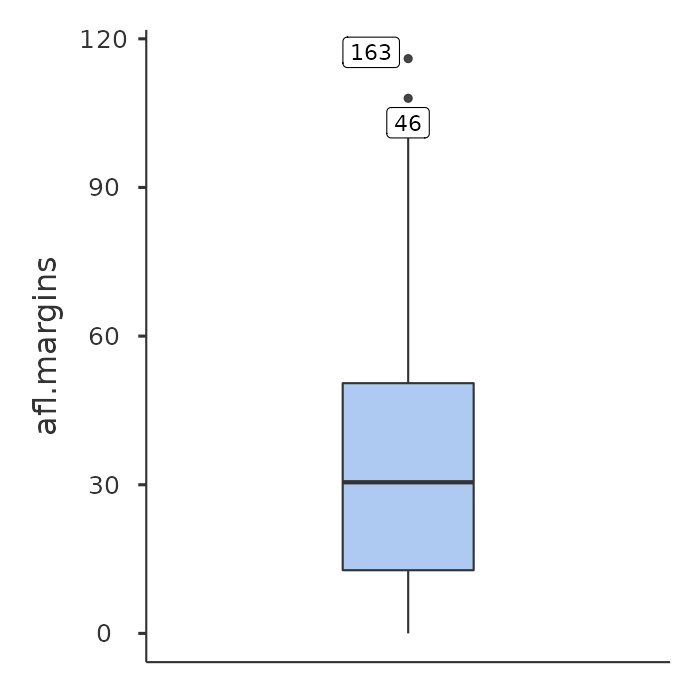
\includegraphics{./images/fig5-4.png} \hfill{}

\caption{\label{fig-fig5-4}A box plot of the afl.margins variable
plotted in jamovi}

\end{figure}

The easiest way to describe what a boxplot looks like is just to draw
one. Click on the `Box plot' check box and you will get the plot shown
on the lower right of Figure~\ref{fig-fig5-4}. jamovi has drawn the most
basic boxplot possible. When you look at this plot this is how you
should interpret it: the thick line in the middle of the box is the
median; the box itself spans the range from the 25th percentile to the
75th percentile; and the ``whiskers'' go out to the most extreme data
point that doesn't exceed a certain bound. By default, this value is 1.5
times the interquartile range (IQR), calculated as 25th percentile -
(1.5*IQR) for the lower boundary, and 75th percentile + (1.5*IQR) for
the upper boundary. Any observation whose value falls outside this range
is plotted as a circle or dot instead of being covered by the whiskers,
and is commonly referred to as an \textbf{outlier}. For our AFL margins
data there are two observations that fall outside this range, and these
observations are plotted as dots (the upper boundary is 107, and looking
over the data column in the spreadsheet there are two observations with
values higher than this, 108 and 116, so these are the dots).

\hypertarget{violin-plots}{%
\subsection{Violin plots}\label{violin-plots}}

\begin{figure}

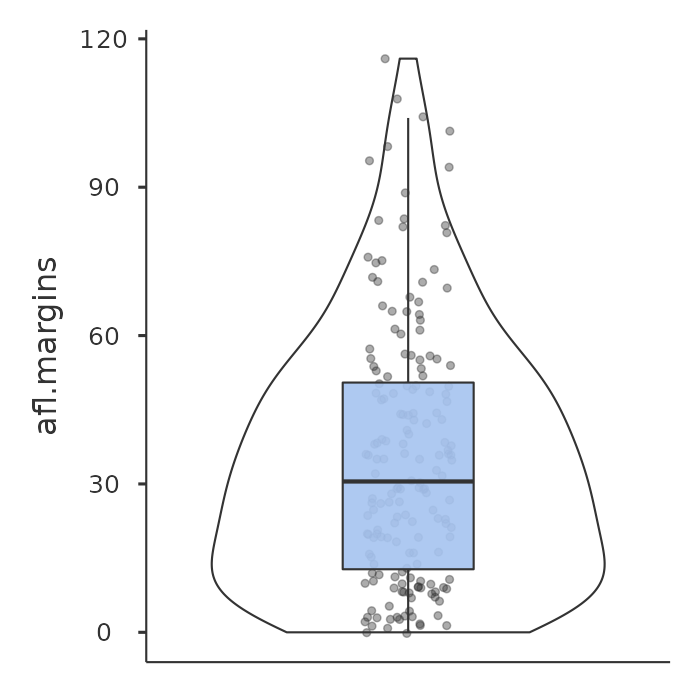
\includegraphics{./images/fig5-5.png} \hfill{}

\caption{\label{fig-fig5-5}A violin plot of the afl.margins variable
plotted in jamovi, also showing a box plot and data points}

\end{figure}

A variation to the traditional box plot is the violin plot. Violin plots
are similar to box plots except that they also show the kernel
probability density of the data at different values. Typically, violin
plots will include a marker for the median of the data and a box
indicating the interquartile range, as in standard box plots. In jamovi
you can achieve this sort of functionality by checking both the `Violin'
and the `Box plot' check boxes. See Figure~\ref{fig-fig5-5}, which also
has the `Data' check box turned on to show the actual data points on the
plot. This does tend to make the graph a bit too busy though, in my
opinion. Clarity is simplicity, so in practice it might be better to
just use a simple box plot.

\hypertarget{drawing-multiple-boxplots}{%
\subsection{Drawing multiple boxplots}\label{drawing-multiple-boxplots}}

One last thing. What if you want to draw multiple boxplots at once?
Suppose, for instance, I wanted separate boxplots showing the AFL
margins not just for 2010 but for every year between 1987 and 2010. To
do that the first thing we'll have to do is find the data. These are
stored in the \textbf{aflmarginbyyear.csv} file. So let's load it into
jamovi and see what is in it. You will see that it is a pretty big data
set. It contains 4296 games and the variables that we're interested in.
What we want to do is have jamovi draw boxplots for the margin variable,
but plotted separately for each year. The way to do this is to move the
year variable across into the `Split by' box, as in
Figure~\ref{fig-fig5-6}.

\begin{figure}

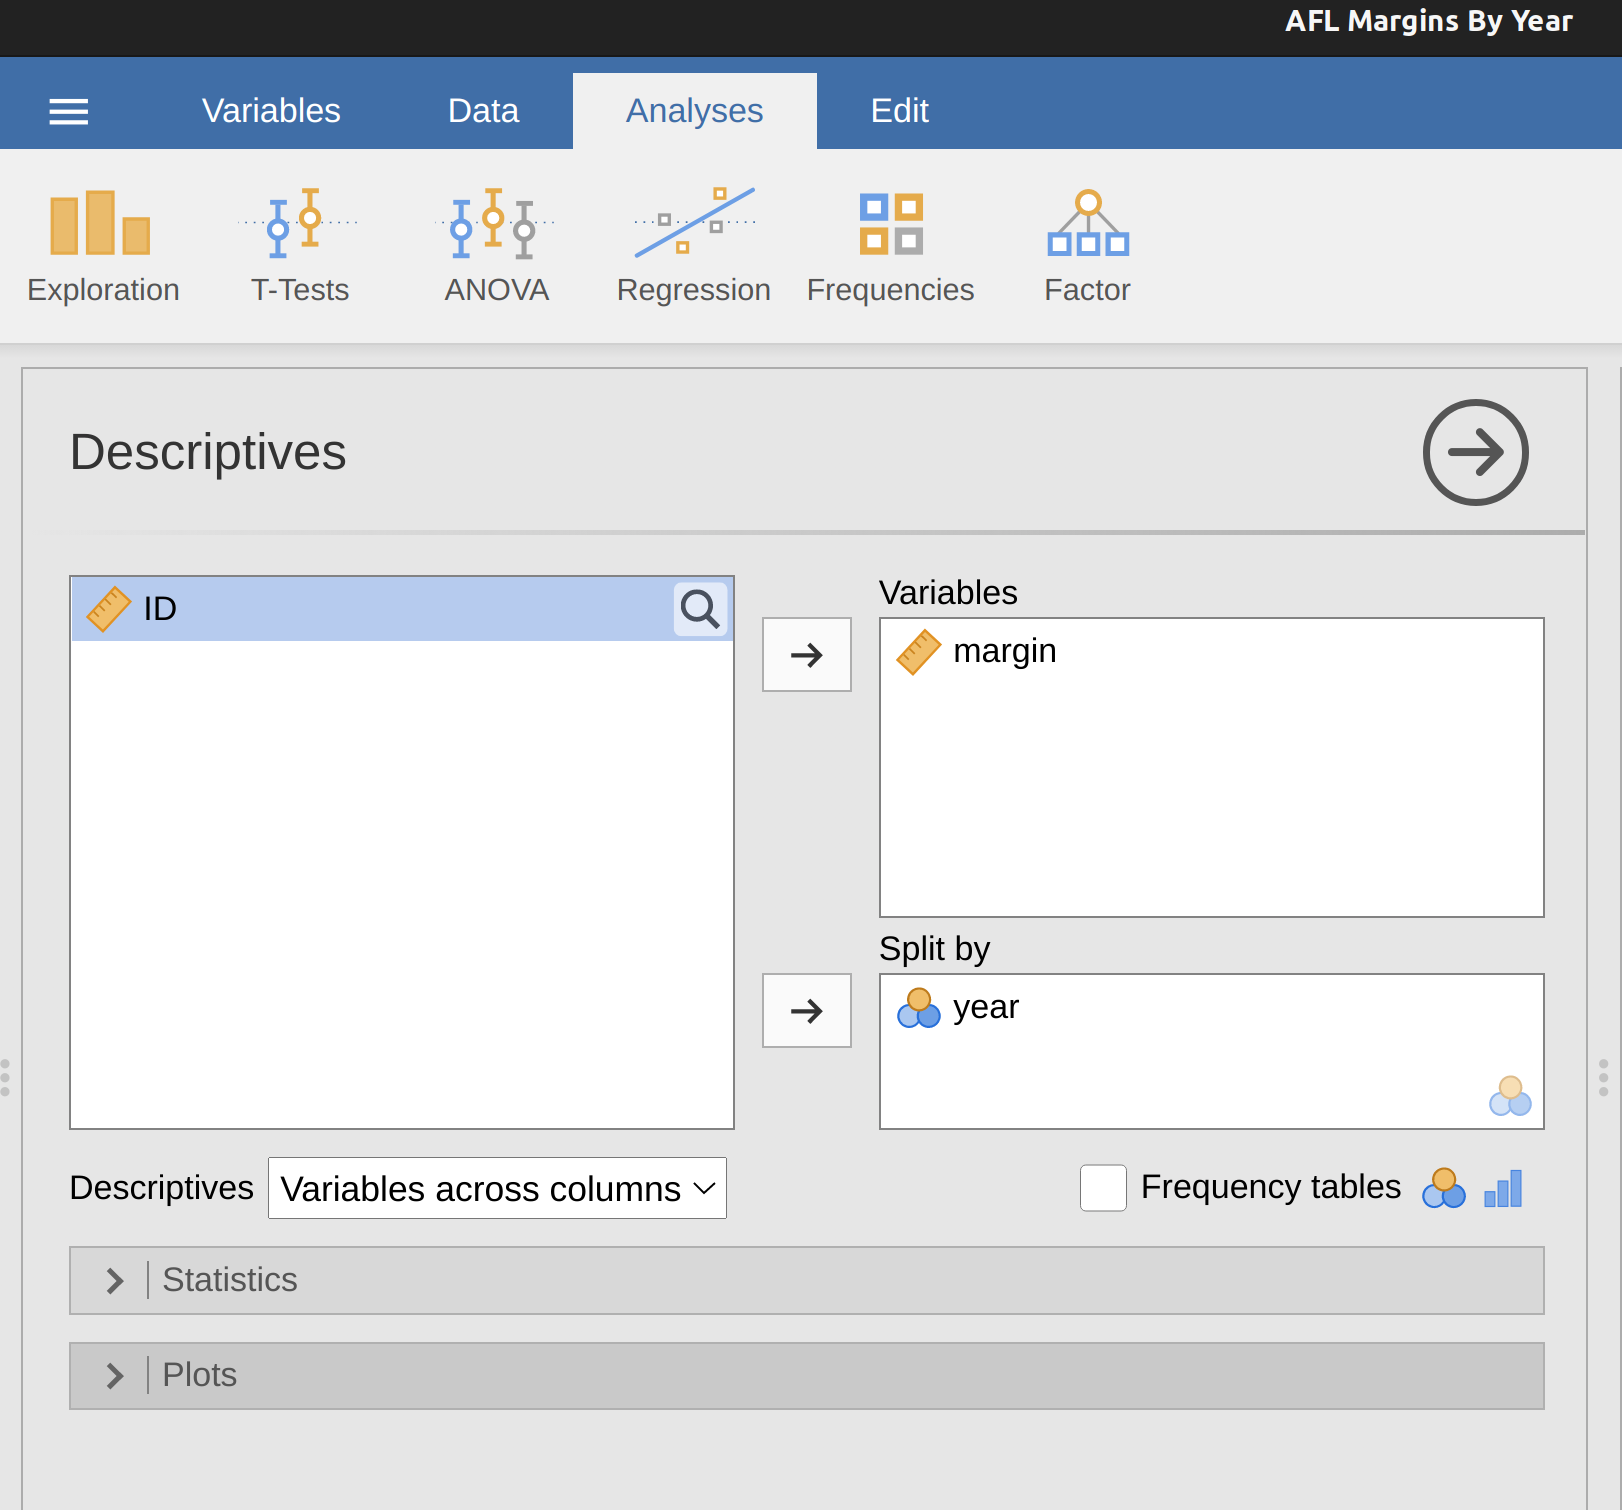
\includegraphics{./images/fig5-6.png} \hfill{}

\caption{\label{fig-fig5-6}jamovi screen shot showing the `Split by'
window}

\end{figure}

The result is shown in Figure~\ref{fig-fig5-7}. This version of the box
plot, split by year, gives a sense of why it's sometimes useful to
choose box plots instead of histograms. It's possible to get a good
sense of what the data look like from year to year without getting
overwhelmed with too much detail. Now imagine what would have happened
if I'd tried to cram 24 histograms into this space: no chance at all
that the reader is going to learn anything useful.

\begin{figure}

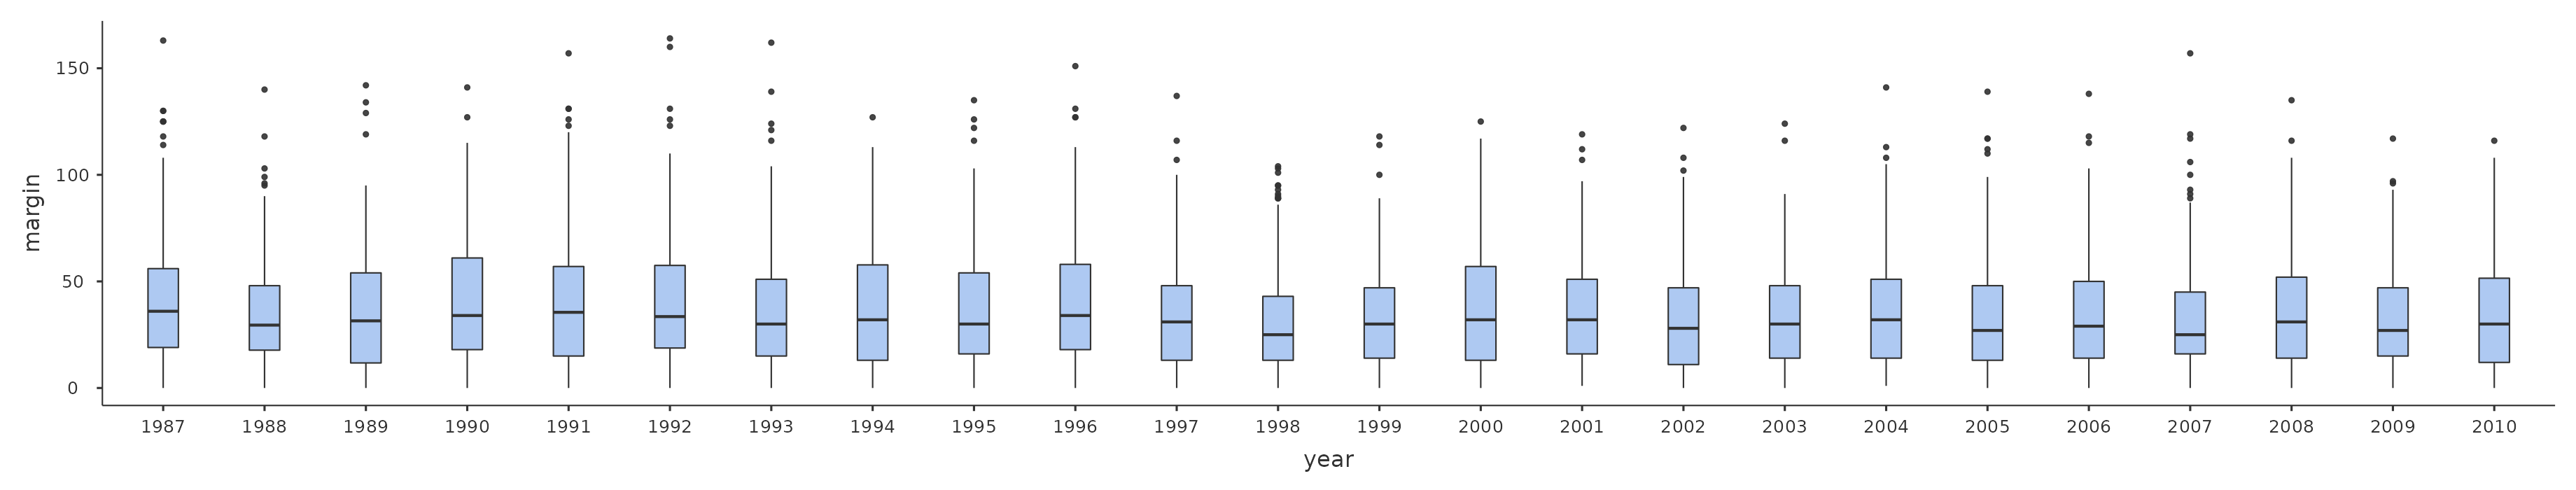
\includegraphics{./images/fig5-7.png} \hfill{}

\caption{\label{fig-fig5-7}Multiple boxplots plotted in jamovi, for the
margin by year variables}

\end{figure}

\hypertarget{sec-Using-box-plots-to-detect-outliers}{%
\subsection{Using box plots to detect
outliers}\label{sec-Using-box-plots-to-detect-outliers}}

Because the boxplot automatically separates out those observations that
lie outside a certain range, depicting them with a dot in jamovi, people
often use them as an informal method for detecting \textbf{outliers}:
observations that are ``suspiciously'' distant from the rest of the
data. Here's an example. Suppose that I'd drawn the boxplot for the AFL
margins data and it came up looking like Figure~\ref{fig-fig5-8}. It's
pretty clear that something funny is going on with two of the
observations. Apparently, there were two games in which the margin was
over 300 points! That doesn't sound right to me. Now that I've become
suspicious it's time to look a bit more closely at the data. In jamovi
you can quickly find out which of these observations are suspicious and
then you can go back to the raw data to see if there has been a mistake
in data entry. One way to do this is to tell jamovi to label the
outliers, by checking the box next to the Box plot check box. This adds
a row number label next to the outlier in the boxplot, so you can go
look at that row and find the extreme value. Another, more flexible way,
is to set up a filter so that only those observations with values over a
certain threshold are included. In our example, the threshold is over
300, so that is the filter we will create. First, click on the `Filters'
button at the top of the jamovi window, and then type `margin
\textgreater{} 300' into the filter field, as in
Figure~\ref{fig-fig5-9}.

\begin{figure}

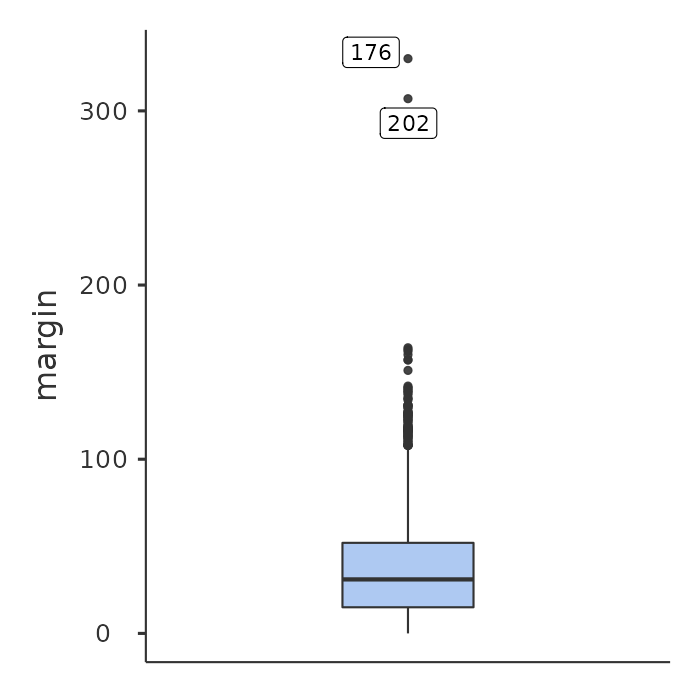
\includegraphics{./images/fig5-8.png} \hfill{}

\caption{\label{fig-fig5-8}A boxplot showing two very suspicious
outliers!}

\end{figure}

This filter creates a new column in the spreadsheet view where only
those observations that pass the filter are included. One neat way to
quickly identify which observations these are is to tell jamovi to
produce a `Frequency table' (in the `Exploration' - `Descriptives'
window) for the ID variable (which must be a nominal variable otherwise
the Frequency table is not produced). In Figure~\ref{fig-fig5-10} you
can see that the ID values for the observations where the margin was
over 300 are 14 and 134. These are suspicious cases, or observations,
where you should go back to the original data source to find out what is
going on.

\begin{figure}

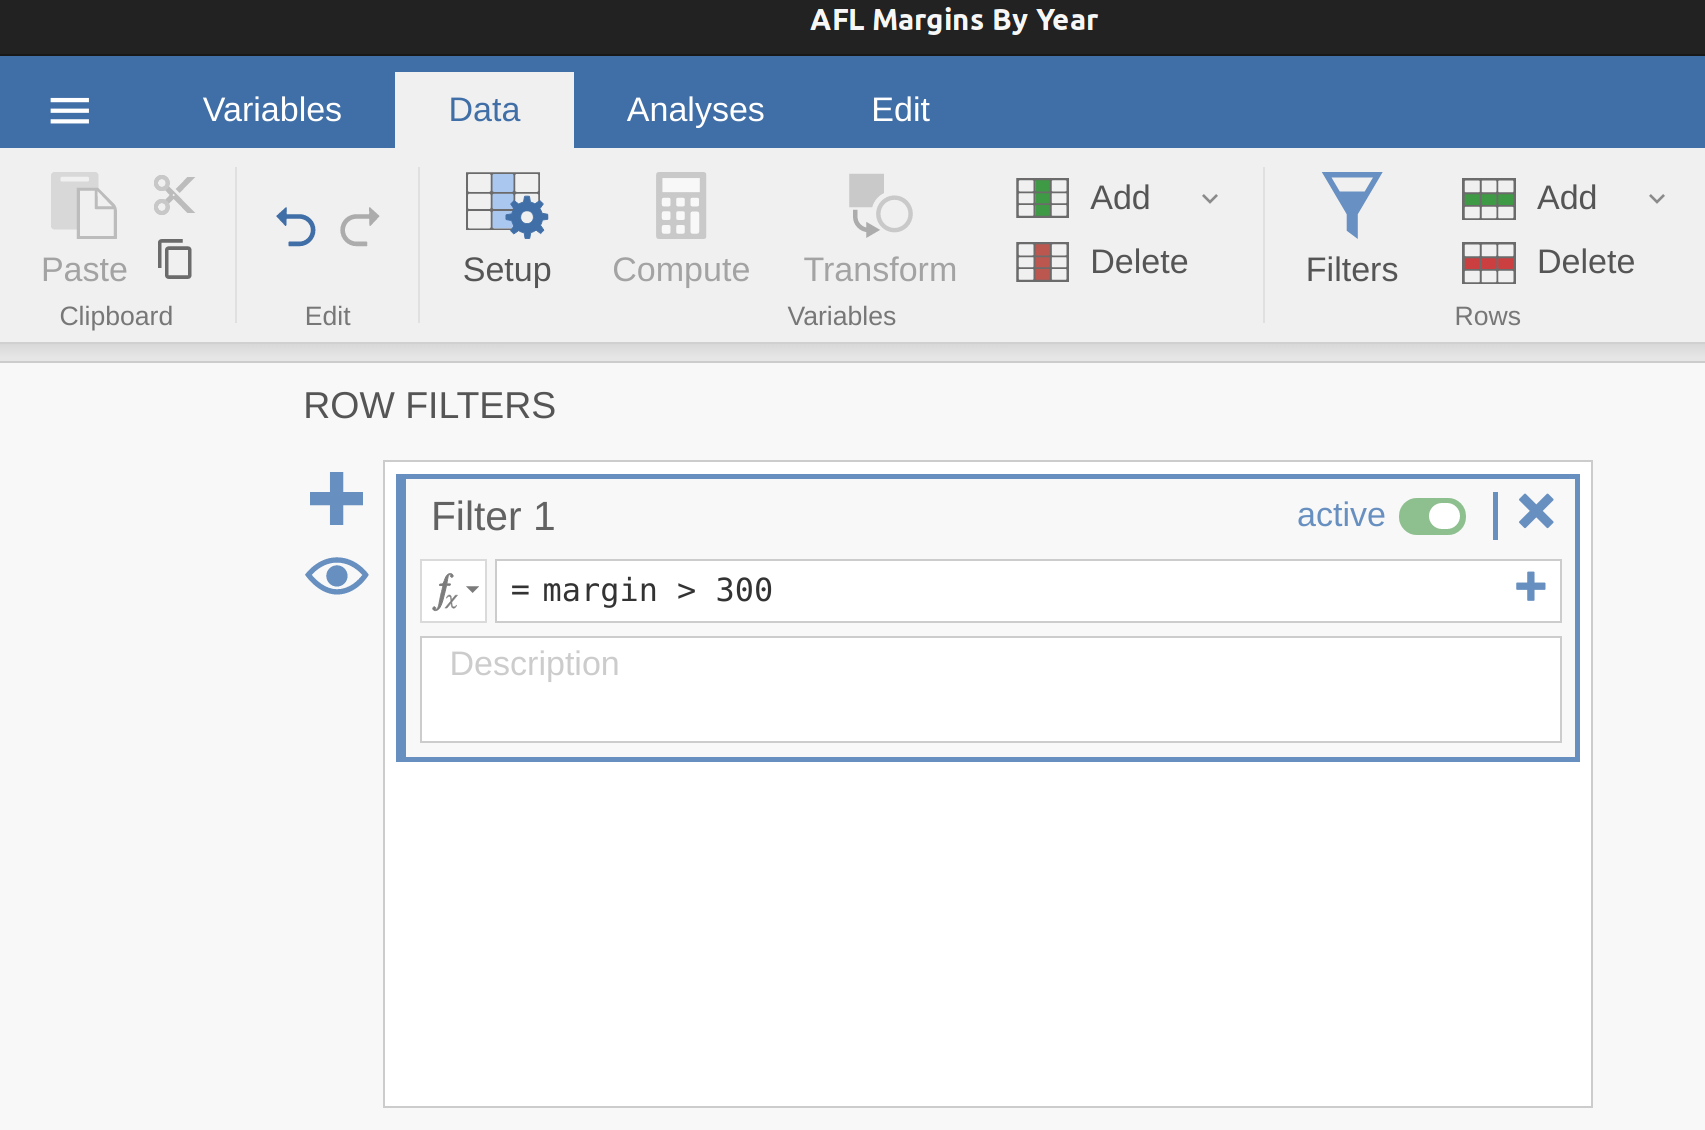
\includegraphics{./images/fig5-9.png} \hfill{}

\caption{\label{fig-fig5-9}The jamovi filter screen}

\end{figure}

\begin{figure}

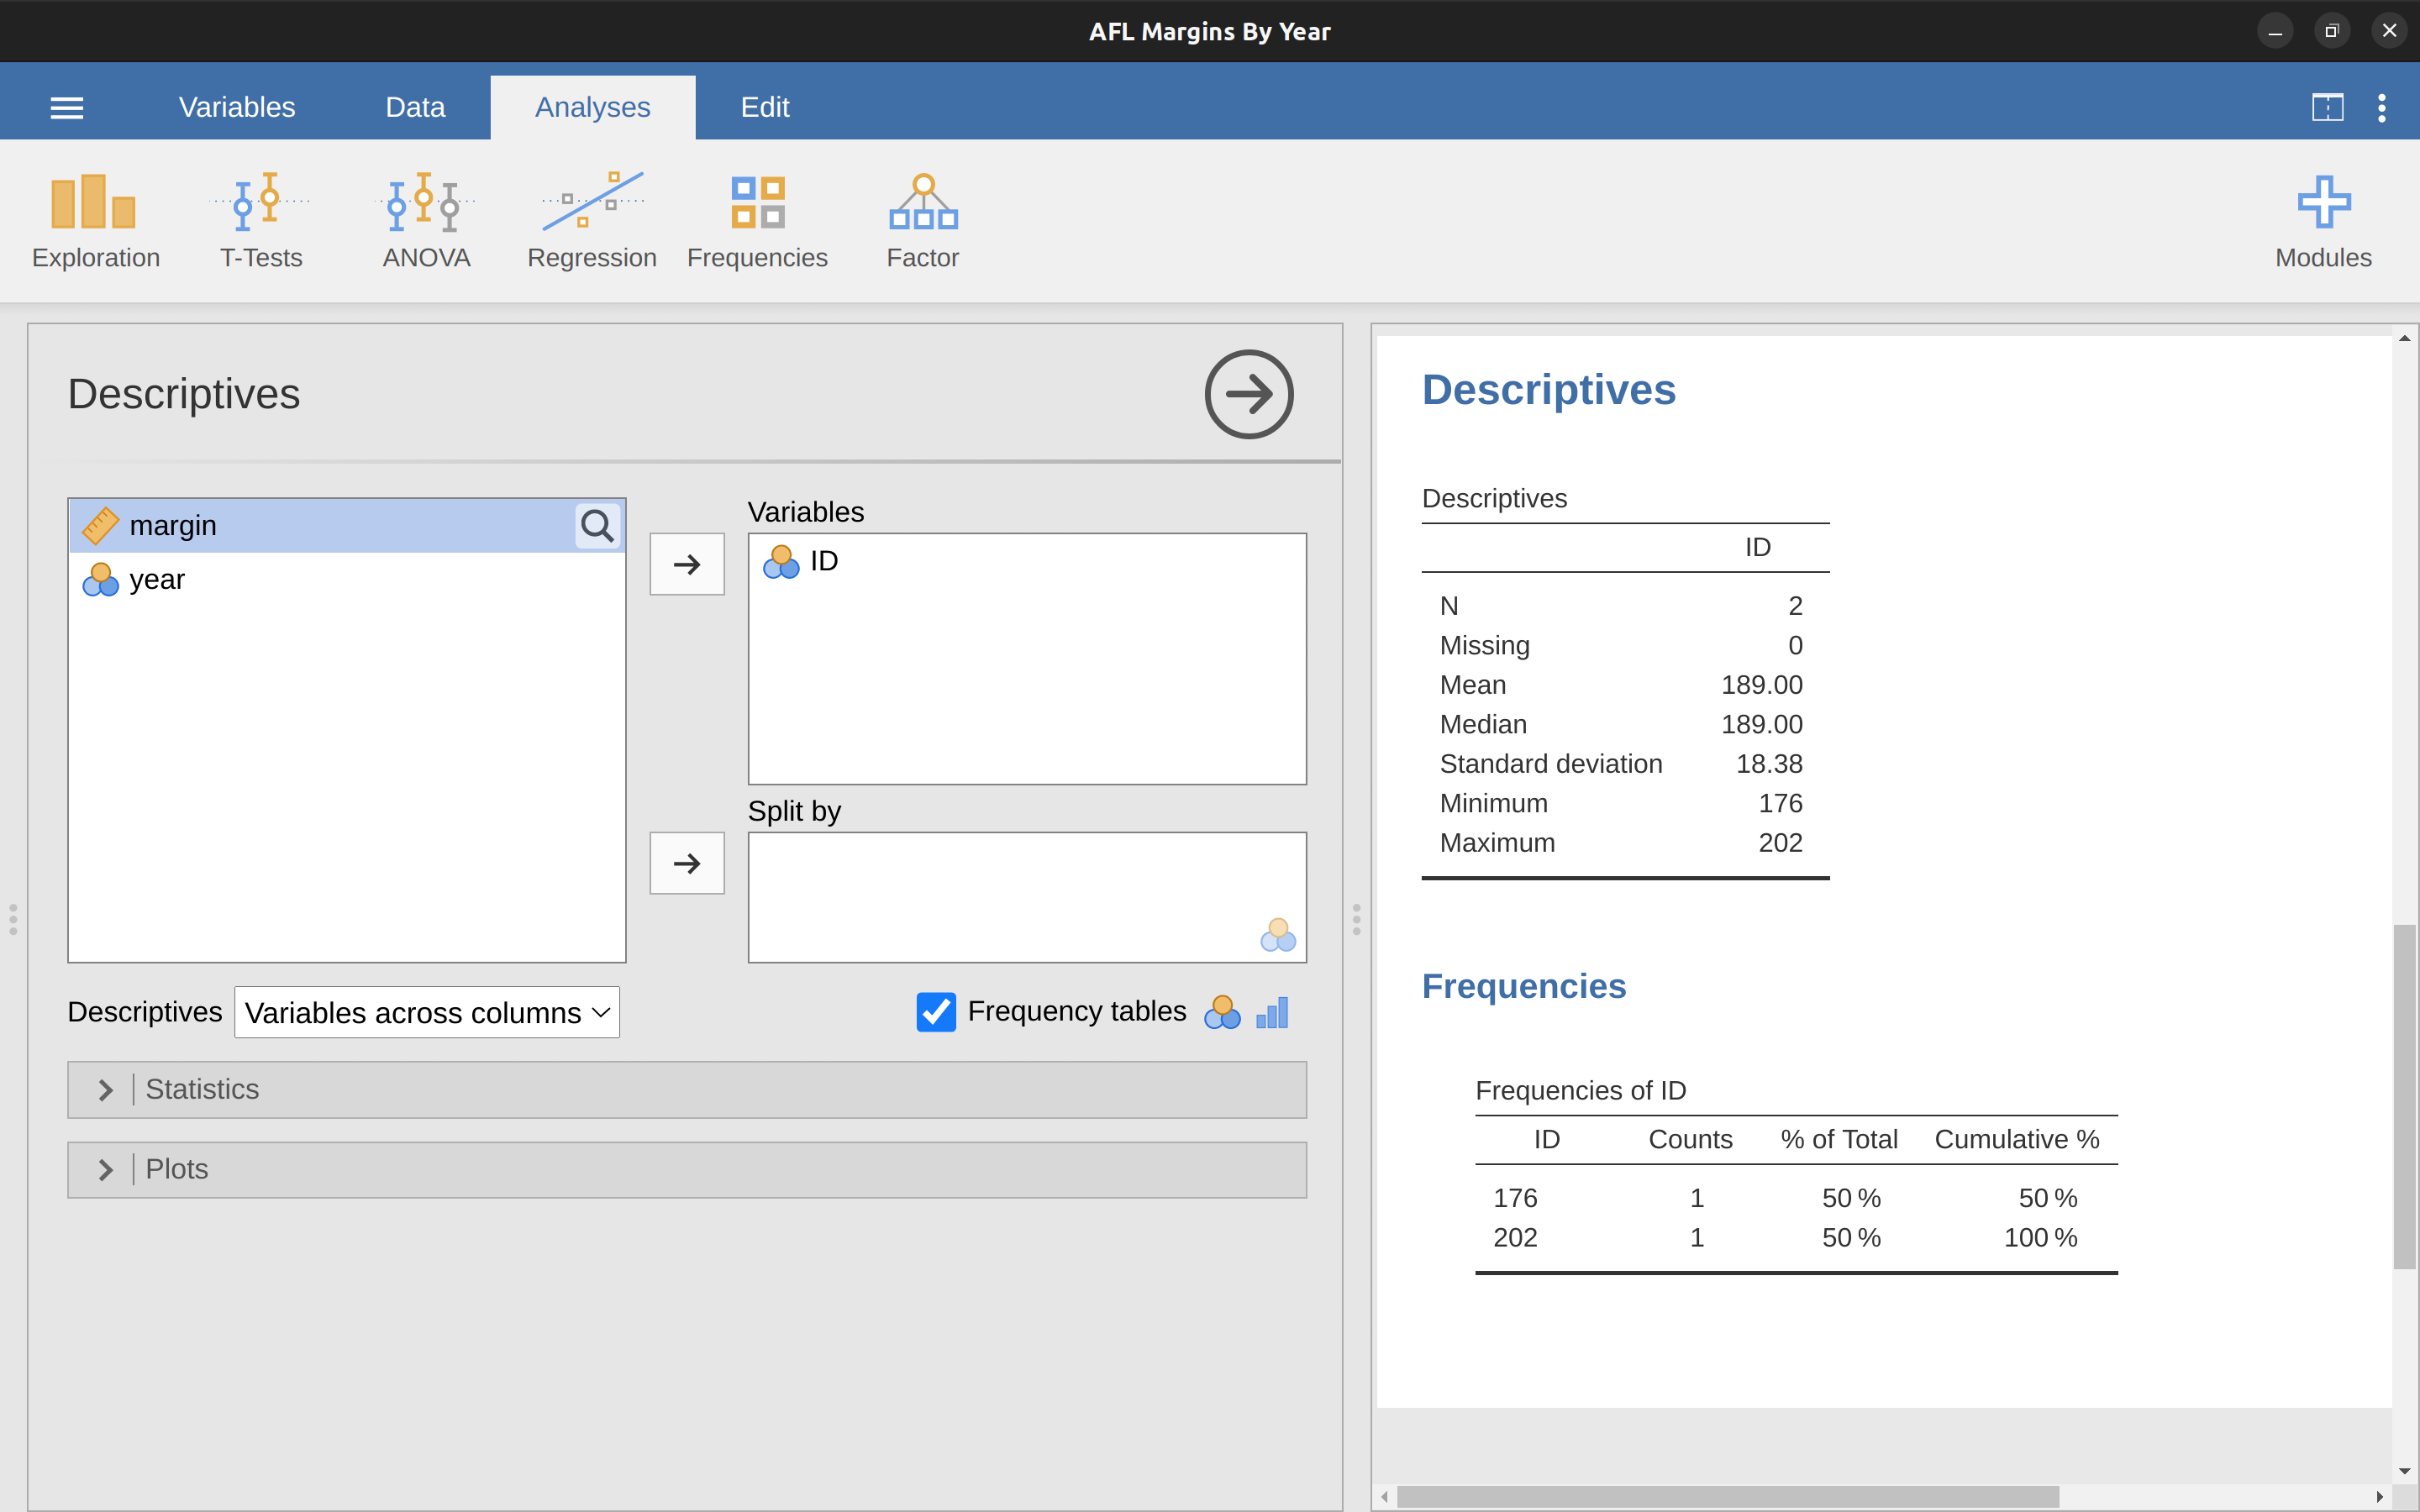
\includegraphics{./images/fig5-10.png} \hfill{}

\caption{\label{fig-fig5-10}Frequency table for ID showing the ID
numbers for the two suspicious outliers, 14 and 134}

\end{figure}

Usually you find that someone has just typed in the wrong number. Whilst
this might seem like a silly example, I should stress that this kind of
thing actually happens a lot. Real world data sets are often riddled
with stupid errors, especially when someone had to type something into a
computer at some point. In fact, there's actually a name for this phase
of data analysis and in practice it can take up a huge chunk of our
time: data cleaning. It involves searching for typing mistakes
(``typos''), missing data and all sorts of other obnoxious errors in raw
data files.

For less extreme values, even if they are flagged in a a boxplot as
outliers, the decision about whether to include outliers or exclude them
in any analysis depends heavily on why you think the data look they way
they do and what you want to use the data for. You really need to
exercise good judgement here. If the outlier looks legitimate to you,
then keep it. In any case, I'll return to the topic again in
Section~\ref{sec-Model-checking} in
Chapter~\ref{sec-Correlation-and-linear-regression}.

\hypertarget{sec-Bar-graphs}{%
\section{Bar graphs}\label{sec-Bar-graphs}}

Another form of graph that you often want to plot is the \textbf{bar
graph}. Let's use the afl.finalists data set with the afl.finalists
variable that I introduced in Section~\ref{sec-Mode}. What I want to do
is draw a bar graph that displays the number of finals that each team
has played in over the time spanned by the afl.finalists data set. There
are lots of teams, but I am particularly interested in just four:
Brisbane, Carlton, Fremantle and Richmond. So the first step is to set
up a filter so just those four teams are included in the bar graph. This
is straightforward in jamovi and you can do it by using the `Filters'
function that we used previously. Open up the `Filters' screen and type
in the following:

afl.finalists \(==\) `Brisbane' or afl.finalists \(==\) `Carlton' or
afl.finalists \(==\) `Fremantle' or afl.finalists \(==\) `Richmond'
\footnote{jamovi uses the symbol ``\(==\)'' here to mean ``matches''.}

When you have done this you will see, in the `Data' view, that jamovi
has filtered out all values apart from those we have specified. Next,
open up the `Exploration' - `Descriptives' window and click on the `Bar
plot' check box (remember to move the `afl.finalists' variable across
into the `Variables' box so that jamovi knows which variable to use).
You should then get a bar graph, something like that shown in
Figure~\ref{fig-fig5-11}.

\begin{figure}

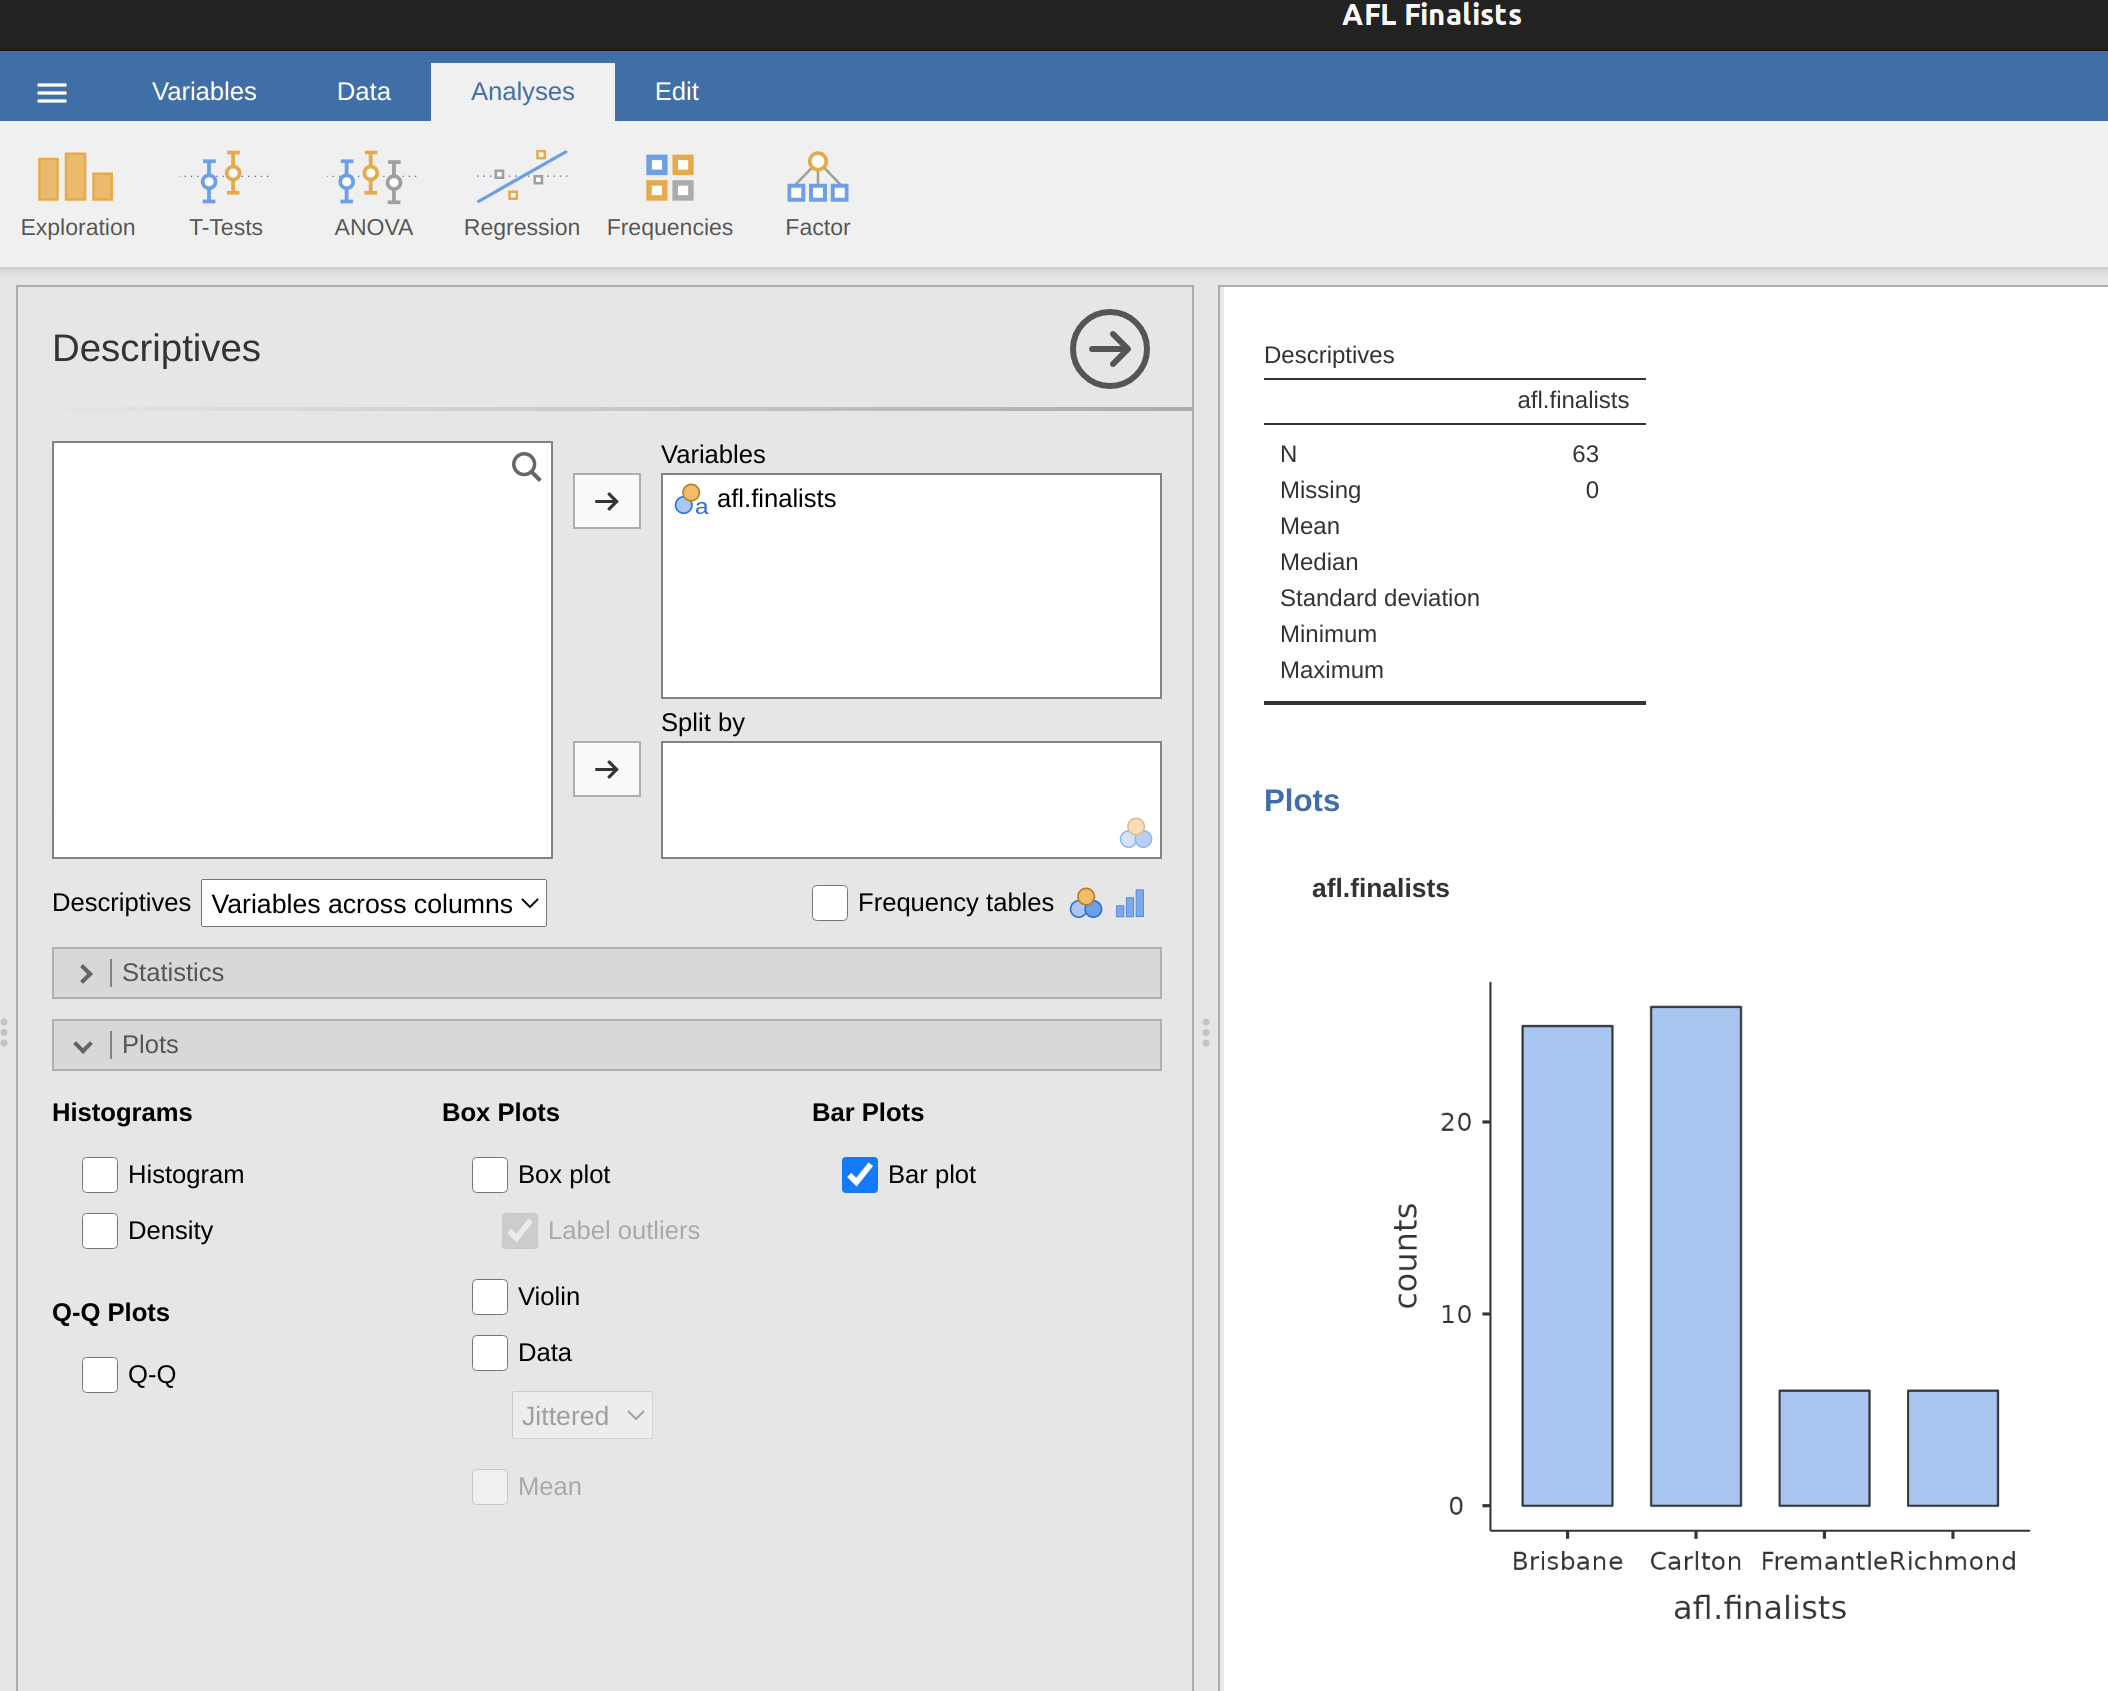
\includegraphics{./images/fig5-11.png} \hfill{}

\caption{\label{fig-fig5-11}Filtering to include just four AFL teams,
and drawing a bar plot in jamovi}

\end{figure}

\hypertarget{saving-image-files-using-jamovi}{%
\section{Saving image files using
jamovi}\label{saving-image-files-using-jamovi}}

Hold on, you might be thinking. What's the good of being able to draw
pretty pictures in jamovi if I can't save them and send them to friends
to brag about how awesome my data is? How do I save the picture?
Simples. Just right click on the plot image and export it to a file,
either as `png', `eps', `svg' or `pdf'. These formats all produce nice
images that you can then send to your friends, or include in your
assignments or papers.

\hypertarget{summary-3}{%
\section{Summary}\label{summary-3}}

Perhaps I'm a simple minded person, but I love pictures. Every time I
write a new scientific paper one of the first things I do is sit down
and think about what the pictures will be. In my head an article is
really just a sequence of pictures linked together by a story. All the
rest of it is just window dressing. What I'm really trying to say here
is that the human visual system is a very powerful data analysis tool.
Give it the right kind of information and it will supply a human reader
with a massive amount of knowledge very quickly. Not for nothing do we
have the saying ``a picture is worth a thousand words''. With that in
mind, I think that this is one of the most important chapters in the
book. The topics covered were:

\begin{itemize}
\tightlist
\item
  \emph{Common plots}. Much of the chapter was focused on standard
  graphs that statisticians like to produce:
  \protect\hyperlink{sec-Histograms}{Histograms},
  \protect\hyperlink{boxplots}{Boxplots} and
  \protect\hyperlink{sec-Bar-graphs}{Bar graphs}
\item
  \protect\hyperlink{saving-image-files-using-jamovi}{Saving image files
  using jamovi}. Importantly, we also covered how to export your
  pictures.
\end{itemize}

One final thing to point out. Whilst jamovi produces some really neat
default graphics, editing the plots is currently not possible. For more
advanced graphics and plotting capability the packages available in R
are much more powerful. One of the most popular graphics systems is
provided by the ggplot2 package (see https://ggplot2.tidyverse.org/),
which is loosely based on ``The grammar of graphics'' (Wilkinson et al.,
2006). It's not for novices. You need to have a pretty good grasp of R
before you can start using it, and even then it takes a while to really
get the hang of it. But when you're ready it's worth taking the time to
teach yourself, because it's a much more powerful and cleaner system.

\begin{center}\rule{0.5\linewidth}{0.5pt}\end{center}

\hypertarget{sec-Pragmatic-matters}{%
\chapter{Pragmatic matters}\label{sec-Pragmatic-matters}}

\begin{quote}
\emph{The garden of life never seems to confine itself to the plots
philosophers have laid out for its convenience. Maybe a few more
tractors would do the trick.}\\
-- Roger Zelazny\footnote{The quote comes from Home is the Hangman,
  published in 1975.}
\end{quote}

This is a somewhat strange chapter, even by my standards. My goal in
this chapter is to talk a bit more honestly about the realities of
working with data than you'll see anywhere else in the book. The problem
with real world data sets is that they are \emph{messy}. Very often the
data file that you start out with doesn't have the variables stored in
the right format for the analysis you want to do. Sometimes there might
be a lot of missing values in your data set. Sometimes you only want to
analyse a subset of the data. Et cetera. In other words, there's a lot
of \textbf{data manipulation} that you need to do just to get the
variables in your data set into the format that you need it. The purpose
of this chapter is to provide a basic introduction to these pragmatic
topics. Although the chapter is motivated by the kinds of practical
issues that arise when manipulating real data, I'll stick with the
practice that I've adopted through most of the book and rely on very
small, toy data sets that illustrate the underlying issue. Because this
chapter is essentially a collection of techniques and doesn't tell a
single coherent story, it may be useful to start with a list of topics:

\begin{itemize}
\tightlist
\item
  \protect\hyperlink{sec-Tabulating-and-cross-tabulating-data}{Tabulating
  and cross-tabulating data}
\item
  \protect\hyperlink{logical-expressions-in-jamovi}{Logical expressions
  in jamovi}
\item
  \protect\hyperlink{sec-Transforming-and-recoding-a-variable}{Transforming
  and recoding a variable}
\item
  \protect\hyperlink{a-few-more-mathematical-functions-and-operations}{A
  few more mathematical functions and operations}
\item
  \protect\hyperlink{extracting-a-subset-of-the-data}{Extracting a
  subset of the data}
\end{itemize}

As you can see, the list of topics that the chapter covers is pretty
broad, and there's a lot of content there. Even though this is one of
the longest and hardest chapters in the book, I'm really only scratching
the surface of several fairly different and important topics. My advice,
as usual, is to read through the chapter once and try to follow as much
of it as you can. Don't worry too much if you can't grasp it all at
once, especially the later sections. The rest of the book is only
lightly reliant on this chapter so you can get away with just
understanding the basics. However, what you'll probably find is that
later on you'll need to flick back to this chapter in order to
understand some of the concepts that I refer to here.

\hypertarget{sec-Tabulating-and-cross-tabulating-data}{%
\section{Tabulating and cross-tabulating
data}\label{sec-Tabulating-and-cross-tabulating-data}}

A very common task when analysing data is the construction of frequency
tables, or crosstabulation of one variable against another. These tasks
can be achieved in jamovi and I'll show you how in this section.

\hypertarget{creating-tables-for-single-variables}{%
\subsection{Creating tables for single
variables}\label{creating-tables-for-single-variables}}

Let's start with a simple example. As the father of a small child I
naturally spend a lot of time watching TV shows like In the \emph{Night
Garden}. In the nightgarden.csv file, I've transcribed a short section
of the dialogue. The file contains two variables of interest, speaker
and utterance. Open up this data set in jamovi and take a look at the
data in the `spreadsheet' view. You will see that the data looks
something like this:

`speaker' variable: upsy-daisy upsy-daisy upsy-daisy upsy-daisy
tombliboo tombliboo makka-pakka makka-pakka makka-pakka makka-pakka
`utterance' variable: pip pip onk onk ee oo pip pip onk onk

Looking at this it becomes very clear what happened to my sanity! With
these as my data, one task I might find myself needing to do is
construct a frequency count of the number of words each character speaks
during the show. The jamovi `Descriptives' screen has a check box called
`Frequency tables' which does just this, see Table~\ref{tbl-tab6-1}.

\hypertarget{tbl-tab6-1}{}
 
  \providecommand{\huxb}[2]{\arrayrulecolor[RGB]{#1}\global\arrayrulewidth=#2pt}
  \providecommand{\huxvb}[2]{\color[RGB]{#1}\vrule width #2pt}
  \providecommand{\huxtpad}[1]{\rule{0pt}{#1}}
  \providecommand{\huxbpad}[1]{\rule[-#1]{0pt}{#1}}

\begin{table}[ht]
\caption{\label{tbl-tab6-1}Frequency table for the speaker variable }\tabularnewline

\begin{centerbox}
\begin{threeparttable}
\setlength{\tabcolsep}{0pt}
\begin{tabularx}{0.9\textwidth}{p{0.225\textwidth} p{0.225\textwidth} p{0.225\textwidth} p{0.225\textwidth}}


\hhline{>{\huxb{0, 0, 0}{0.4}}->{\huxb{0, 0, 0}{0.4}}->{\huxb{0, 0, 0}{0.4}}->{\huxb{0, 0, 0}{0.4}}-}
\arrayrulecolor{black}

\multicolumn{1}{!{\huxvb{0, 0, 0}{0}}p{0.225\textwidth}!{\huxvb{0, 0, 0}{0}}}{\cellcolor[RGB]{242, 242, 242}\hspace{0pt}\parbox[b]{0.225\textwidth-0pt-6pt}{\huxtpad{6pt + 1em}\centering \textbf{levels}\huxbpad{6pt}}} &
\multicolumn{1}{p{0.225\textwidth}!{\huxvb{0, 0, 0}{0}}}{\cellcolor[RGB]{242, 242, 242}\hspace{6pt}\parbox[b]{0.225\textwidth-6pt-6pt}{\huxtpad{6pt + 1em}\centering \textbf{Counts}\huxbpad{6pt}}} &
\multicolumn{1}{p{0.225\textwidth}!{\huxvb{0, 0, 0}{0}}}{\cellcolor[RGB]{242, 242, 242}\hspace{6pt}\parbox[b]{0.225\textwidth-6pt-6pt}{\huxtpad{6pt + 1em}\centering \textbf{\(\%\) of Total}\huxbpad{6pt}}} &
\multicolumn{1}{p{0.225\textwidth}!{\huxvb{0, 0, 0}{0}}}{\cellcolor[RGB]{242, 242, 242}\hspace{6pt}\parbox[b]{0.225\textwidth-6pt-0pt}{\huxtpad{6pt + 1em}\centering \textbf{Cumulative \(\%\)}\huxbpad{6pt}}} \tabularnewline[-0.5pt]


\hhline{>{\huxb{0, 0, 0}{0.4}}->{\huxb{0, 0, 0}{0.4}}->{\huxb{0, 0, 0}{0.4}}->{\huxb{0, 0, 0}{0.4}}-}
\arrayrulecolor{black}

\multicolumn{1}{!{\huxvb{0, 0, 0}{0}}p{0.225\textwidth}!{\huxvb{0, 0, 0}{0}}}{\hspace{0pt}\parbox[b]{0.225\textwidth-0pt-6pt}{\huxtpad{6pt + 1em}\centering makka-pakka\huxbpad{6pt}}} &
\multicolumn{1}{p{0.225\textwidth}!{\huxvb{0, 0, 0}{0}}}{\hspace{6pt}\parbox[b]{0.225\textwidth-6pt-6pt}{\huxtpad{6pt + 1em}\centering 4\huxbpad{6pt}}} &
\multicolumn{1}{p{0.225\textwidth}!{\huxvb{0, 0, 0}{0}}}{\hspace{6pt}\parbox[b]{0.225\textwidth-6pt-6pt}{\huxtpad{6pt + 1em}\centering 40\(\%\)\huxbpad{6pt}}} &
\multicolumn{1}{p{0.225\textwidth}!{\huxvb{0, 0, 0}{0}}}{\hspace{6pt}\parbox[b]{0.225\textwidth-6pt-0pt}{\huxtpad{6pt + 1em}\centering 40\(\%\)\huxbpad{6pt}}} \tabularnewline[-0.5pt]


\hhline{}
\arrayrulecolor{black}

\multicolumn{1}{!{\huxvb{0, 0, 0}{0}}p{0.225\textwidth}!{\huxvb{0, 0, 0}{0}}}{\cellcolor[RGB]{242, 242, 242}\hspace{0pt}\parbox[b]{0.225\textwidth-0pt-6pt}{\huxtpad{6pt + 1em}\centering tombliboo\huxbpad{6pt}}} &
\multicolumn{1}{p{0.225\textwidth}!{\huxvb{0, 0, 0}{0}}}{\cellcolor[RGB]{242, 242, 242}\hspace{6pt}\parbox[b]{0.225\textwidth-6pt-6pt}{\huxtpad{6pt + 1em}\centering 2\huxbpad{6pt}}} &
\multicolumn{1}{p{0.225\textwidth}!{\huxvb{0, 0, 0}{0}}}{\cellcolor[RGB]{242, 242, 242}\hspace{6pt}\parbox[b]{0.225\textwidth-6pt-6pt}{\huxtpad{6pt + 1em}\centering 20\(\%\)\huxbpad{6pt}}} &
\multicolumn{1}{p{0.225\textwidth}!{\huxvb{0, 0, 0}{0}}}{\cellcolor[RGB]{242, 242, 242}\hspace{6pt}\parbox[b]{0.225\textwidth-6pt-0pt}{\huxtpad{6pt + 1em}\centering 60\(\%\)\huxbpad{6pt}}} \tabularnewline[-0.5pt]


\hhline{}
\arrayrulecolor{black}

\multicolumn{1}{!{\huxvb{0, 0, 0}{0}}p{0.225\textwidth}!{\huxvb{0, 0, 0}{0}}}{\hspace{0pt}\parbox[b]{0.225\textwidth-0pt-6pt}{\huxtpad{6pt + 1em}\centering upsy-daisy\huxbpad{6pt}}} &
\multicolumn{1}{p{0.225\textwidth}!{\huxvb{0, 0, 0}{0}}}{\hspace{6pt}\parbox[b]{0.225\textwidth-6pt-6pt}{\huxtpad{6pt + 1em}\centering 4\huxbpad{6pt}}} &
\multicolumn{1}{p{0.225\textwidth}!{\huxvb{0, 0, 0}{0}}}{\hspace{6pt}\parbox[b]{0.225\textwidth-6pt-6pt}{\huxtpad{6pt + 1em}\centering 40\(\%\)\huxbpad{6pt}}} &
\multicolumn{1}{p{0.225\textwidth}!{\huxvb{0, 0, 0}{0}}}{\hspace{6pt}\parbox[b]{0.225\textwidth-6pt-0pt}{\huxtpad{6pt + 1em}\centering 100\(\%\)\huxbpad{6pt}}} \tabularnewline[-0.5pt]


\hhline{>{\huxb{0, 0, 0}{0.4}}->{\huxb{0, 0, 0}{0.4}}->{\huxb{0, 0, 0}{0.4}}->{\huxb{0, 0, 0}{0.4}}-}
\arrayrulecolor{black}
\end{tabularx} 

\end{threeparttable}\par\end{centerbox}

\end{table}
 

The output here tells us on the first line that what we're looking at is
a tabulation of the speaker variable. In the `Levels' column it lists
all the different speakers that exist in the data, and in the `Counts'
column it tells you how many times that speaker appears in the data. In
other words, it's a frequency table.

In jamovi, the `Frequency tables' check box will only produce a table
for single variables. For a table of two variables, for example
combining speaker and utterance so that we can see how many times each
speaker said a particular utterance, we need a cross-tabulation or
contingency table. In jamovi you can do this by selecting the
`Frequencies' - `Contingency Tables' - `Independent Samples' analysis,
and moving the speaker variable into the `Rows' box, and the utterances
variable into the `Columns' box. You then should have a contingency
table like the one shown in Figure~\ref{fig-fig6-1}.

\begin{figure}

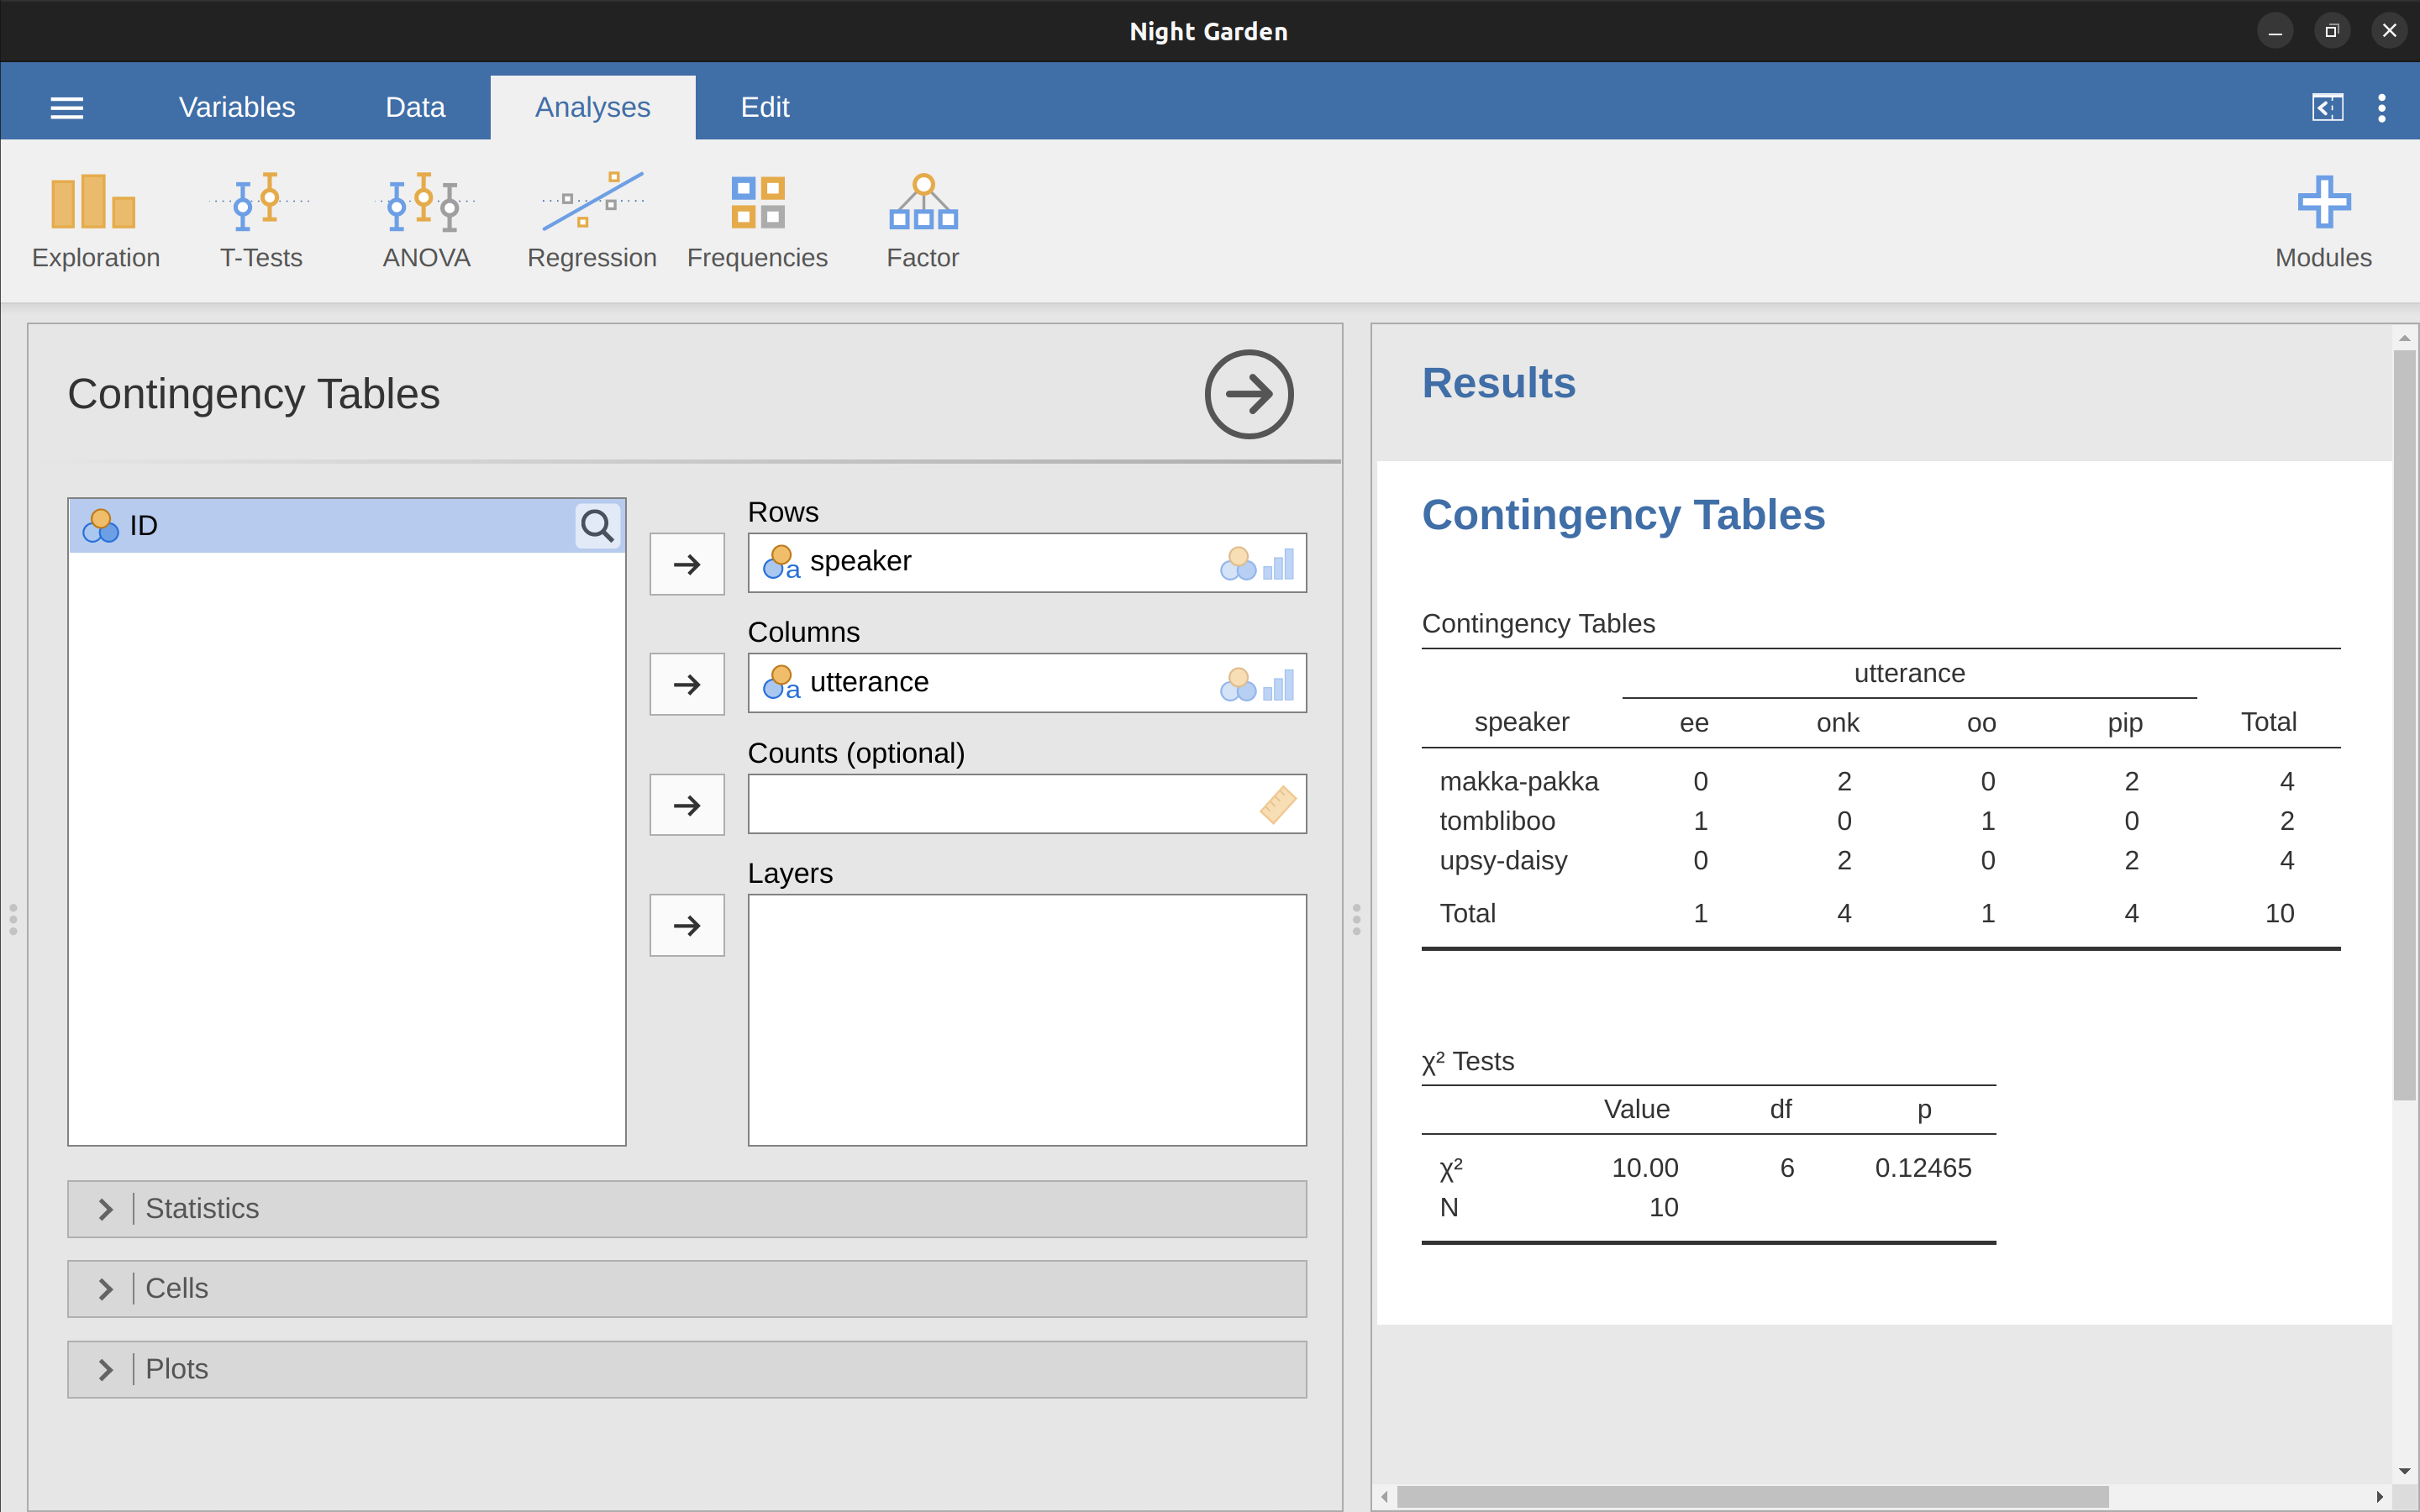
\includegraphics{./images/fig6-1.png} \hfill{}

\caption{\label{fig-fig6-1}Contingency table for the speaker and
utterances variables}

\end{figure}

Don't worry about the ``\(\chi^2\) Tests'' table that is produced. We
are going to cover this later on in
Chapter~\ref{sec-Categorical-data-analysis}. When interpreting the
contingency table remember that these are counts, so the fact that the
first row and second column of numbers corresponds to a value of 2
indicates that Makka-Pakka (row 1) says ``onk'' (column 2) twice in this
data set.

\hypertarget{adding-percentages-to-a-contingency-table}{%
\subsection{Adding percentages to a contingency
table}\label{adding-percentages-to-a-contingency-table}}

The contingency table shown in Figure~\ref{fig-fig6-1} shows a table of
raw frequencies. That is, a count of the total number of cases for
different combinations of levels of the specified variables. However,
often you want your data to be organised in terms of percentages as well
as counts. You can find the check boxes for different percentages under
the `Cells' option in the `Contingency Tables' window. First, click on
the `Row' check box and the Contingency Table in the output window will
change to the one in Figure~\ref{fig-fig6-2}.

\begin{figure}

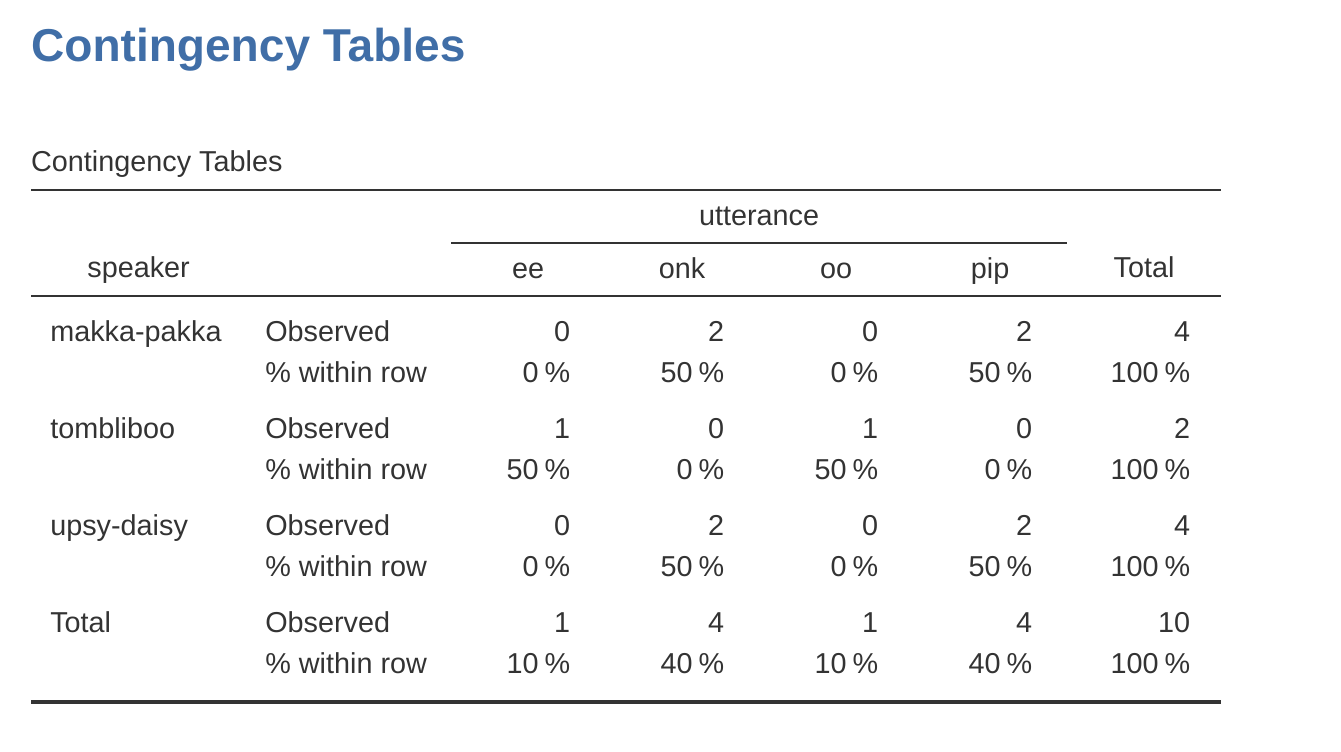
\includegraphics{./images/fig6-2.png} \hfill{}

\caption{\label{fig-fig6-2}Contingency table for the speaker and
utterances variables, with row percentages}

\end{figure}

What we're looking at here is the percentage of utterances made by each
character. In other words, 50\% of Makka-Pakka's utterances are ``pip'',
and the other 50\% are ``onk''. Let's contrast this with the table we
get when we calculate column percentages (uncheck `Row' and check
`Column' in the Cells options window), see Figure~\ref{fig-fig6-3}. In
this version, what we're seeing is the percentage of characters
associated with each utterance. For instance, whenever the utterance
``ee'' is made (in this data set), 100\% of the time it's a Tombliboo
saying it.

\begin{figure}

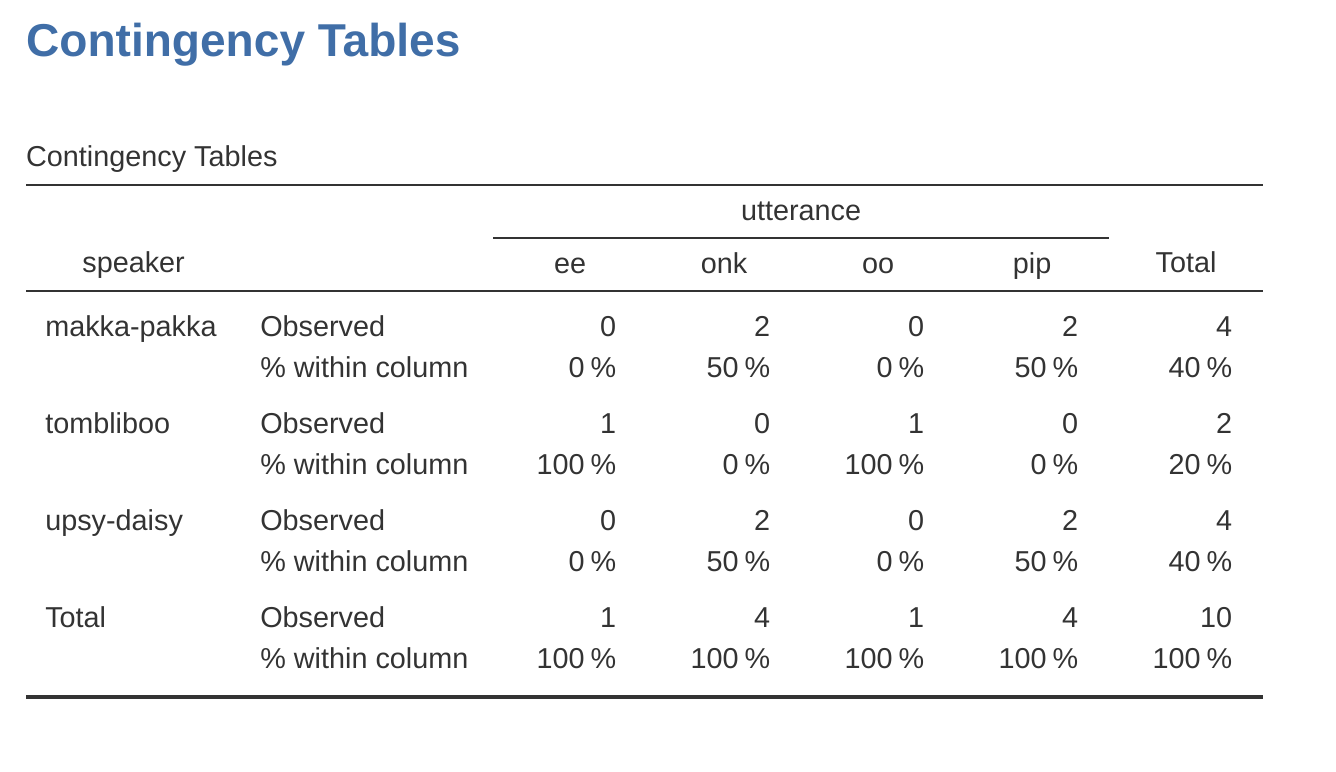
\includegraphics{./images/fig6-3.png} \hfill{}

\caption{\label{fig-fig6-3}Contingency table for the speaker and
utterances variables, with column percentages}

\end{figure}

\hypertarget{logical-expressions-in-jamovi}{%
\section{Logical expressions in
jamovi}\label{logical-expressions-in-jamovi}}

A key concept that a lot of data transformations in jamovi rely on is
the idea of a \textbf{logical value}. A logical value is an assertion
about whether something is true or false. This is implemented in jamovi
in a pretty straightforward way. There are two logical values, namely
TRUE and FALSE. Despite the simplicity, logical values are very useful
things. Let's see how they work.

\hypertarget{assessing-mathematical-truths}{%
\subsection{Assessing mathematical
truths}\label{assessing-mathematical-truths}}

In George Orwell's classic book 1984 one of the slogans used by the
totalitarian Party was ``two plus two equals five''. The idea being that
the political domination of human freedom becomes complete when it is
possible to subvert even the most basic of truths. It's a terrifying
thought, especially when the protagonist Winston Smith finally breaks
down under torture and agrees to the proposition. ``Man is infinitely
malleable'', the book says. I'm pretty sure that this isn't true of
humans\footnote{I offer up my teenage attempts to be ``cool'' as
  evidence that some things just can't be done.} and it's definitely not
true of jamovi. jamovi is not infinitely malleable, it has rather firm
opinions on the topic of what is and isn't true, at least as regards
basic mathematics. If I ask it to calculate \(2 + 2\)\footnote{You can
  do this in the Compute new variable screen, though just calculating 2
  + 2 for every cell of a new variable is not very useful!}, it always
gives the same answer, and it's not bloody 5!

Of course, so far jamovi is just doing the calculations. I haven't asked
it to explicitly assert that \(2 + 2 = 4\) is a true statement. If I
want jamovi to make an explicit judgement, I can use a command like
this: \(2 + 2 == 4\)

What I've done here is use the \textbf{equality operator}, \(==\), to
force jamovi to make a ``true or false'' judgement.\footnote{Note that
  this is a very different operator to the equals operator =. A common
  typo that people make when trying to write logical commands in jamovi
  (or other languages, since the ``= versus =='' distinction is
  important in many computer and statistical programs) is to
  accidentally type = when you really mean ==. Be especially cautious
  with this, I've been programming in various languages since I was a
  teenager and I still screw this up a lot. Hmm. I think I see why I
  wasn't cool as a teenager. And why I'm still not cool.} Okay, let's
see what jamovi thinks of the Party slogan, so type this into the
compute new variable `formula' box:

\[2 + 2 == 5\]

And what do you get? It should be a whole set of `false' values in the
spreadsheet column for your newly computed variable. Booyah! Freedom and
ponies for all! Or something like that. Anyway, it was worth having a
look at what happens if I try to force jamovi to believe that two plus
two is five by making a statement like \(2 + 2 = 5\). I know that if I
do this in another program, say R, then it throws up an error message.
But wait, if you do this in jamovi you get a whole set of `false'
values. So what is going on? Well, it seems that jamovi is being pretty
smart and realises that you are testing whether it is TRUE or FALSE that
\(2 + 2 = 5\), regardless of whether you use the correct
\textbf{equality operator}, \(==\), or the equals sign ``\(=\)''.

Anyway, it was worth having a look at what happens if I try to force
jamovi to believe that two plus two is five by making a statement like
\(2 + 2 = 5\). I know that if I do this in another program, say R, then
it throws up an error message. But wait, if you do this in jamovi you
get a whole set of `false' values. So what is going on? Well, it seems
that jamovi is being pretty smart and realises that you are testing
whether it is TRUE or FALSE that \(2 + 2 = 5\), regardless of whether
you use the correct \textbf{equality operator}, \(==\), or the equals
sign ``\(=\)''.

\hypertarget{logical-operations}{%
\subsection{Logical operations}\label{logical-operations}}

So now we've seen logical operations at work. But so far we've only seen
the simplest possible example. You probably won't be surprised to
discover that we can combine logical operations with other operations
and functions in a more complicated way, like this:
\(3 \times 3 + 4 \times 4 == 5 \times 5\) or this \(SQRT(25) == 5\)

Not only that, but as Table~\ref{tbl-tab6-2} illustrates, there are
several other logical operators that you can use corresponding to some
basic mathematical concepts. Hopefully these are all pretty
self-explanatory. For example, the \textbf{less than} operator
\textless{} checks to see if the number on the left is less than the
number on the right. If it's less, then jamovi returns an answer of
TRUE, but if the two numbers are equal, or if the one on the right is
larger, then jamovi returns an answer of FALSE.

In contrast, the \textbf{less than or equal to} operator \(<=\) will do
exactly what it says. It returns a value of TRUE if the number of the
left hand side is less than or equal to the number on the right hand
side. At this point I hope it's pretty obvious what the \textbf{greater
than} operator \(<\) and the \textbf{greater than or equal to} operator
\(<=\) do!

Next on the list of logical operators is the \textbf{not equal to}
operator != which, as with all the others, does what it says it does. It
returns a value of TRUE when things on either side are not identical to
each other. Therefore, since \(2 + 2\) isn't equal to \(5\), we would
get `true' as the value for our newly computed variable. Try it and see:

\[2 + 2 \text{ != } 5\]

We're not quite done yet. There are three more logical operations that
are worth knowing about, listed in Table~\ref{tbl-tab6-3}. These are the
\textbf{not} operator !, the \textbf{and} operator and, and the
\textbf{or} operator or. Like the other logical operators, their
behaviour is more or less exactly what you'd expect given their names.
For instance, if I ask you to assess the claim that ``either
\(2 + 2 = 4\) or \(2 + 2 = 5\)'' you'd say that it's true. Since it's an
``either-or'' statement, all we need is for one of the two parts to be
true. That's what the or operator does:\footnote{Now, here's a quirk in
  jamovi. When you have simple logical expressions like the ones we have
  already met, e.g.~2 + 2 == 5 then jamovi neatly states `false' (or
  `true') in the corresponding spreadsheet column. Underneath the hood,
  jamovi stores `false' as 0 and `true' as 1. When we have more complex
  logical expressions, such as (2+2 == 4) or (2+2 == 5), then jamovi
  just displays either 0 or 1, depending whether the logical expression
  is evaluated as false, or true.}

\hypertarget{tbl-tab6-2}{}
 
  \providecommand{\huxb}[2]{\arrayrulecolor[RGB]{#1}\global\arrayrulewidth=#2pt}
  \providecommand{\huxvb}[2]{\color[RGB]{#1}\vrule width #2pt}
  \providecommand{\huxtpad}[1]{\rule{0pt}{#1}}
  \providecommand{\huxbpad}[1]{\rule[-#1]{0pt}{#1}}

\begin{table}[ht]
\caption{\label{tbl-tab6-2}Some logical operators }\tabularnewline

\begin{centerbox}
\begin{threeparttable}
\setlength{\tabcolsep}{0pt}
\begin{tabularx}{0.9\textwidth}{p{0.225\textwidth} p{0.225\textwidth} p{0.225\textwidth} p{0.225\textwidth}}


\hhline{>{\huxb{0, 0, 0}{0.4}}->{\huxb{0, 0, 0}{0.4}}->{\huxb{0, 0, 0}{0.4}}->{\huxb{0, 0, 0}{0.4}}-}
\arrayrulecolor{black}

\multicolumn{1}{!{\huxvb{0, 0, 0}{0}}p{0.225\textwidth}!{\huxvb{0, 0, 0}{0}}}{\cellcolor[RGB]{242, 242, 242}\hspace{0pt}\parbox[b]{0.225\textwidth-0pt-6pt}{\huxtpad{6pt + 1em}\centering \textbf{operation}\huxbpad{6pt}}} &
\multicolumn{1}{p{0.225\textwidth}!{\huxvb{0, 0, 0}{0}}}{\cellcolor[RGB]{242, 242, 242}\hspace{6pt}\parbox[b]{0.225\textwidth-6pt-6pt}{\huxtpad{6pt + 1em}\centering \textbf{operator}\huxbpad{6pt}}} &
\multicolumn{1}{p{0.225\textwidth}!{\huxvb{0, 0, 0}{0}}}{\cellcolor[RGB]{242, 242, 242}\hspace{6pt}\parbox[b]{0.225\textwidth-6pt-6pt}{\huxtpad{6pt + 1em}\centering \textbf{example input}\huxbpad{6pt}}} &
\multicolumn{1}{p{0.225\textwidth}!{\huxvb{0, 0, 0}{0}}}{\cellcolor[RGB]{242, 242, 242}\hspace{6pt}\parbox[b]{0.225\textwidth-6pt-0pt}{\huxtpad{6pt + 1em}\centering \textbf{answer}\huxbpad{6pt}}} \tabularnewline[-0.5pt]


\hhline{>{\huxb{0, 0, 0}{0.4}}->{\huxb{0, 0, 0}{0.4}}->{\huxb{0, 0, 0}{0.4}}->{\huxb{0, 0, 0}{0.4}}-}
\arrayrulecolor{black}

\multicolumn{1}{!{\huxvb{0, 0, 0}{0}}p{0.225\textwidth}!{\huxvb{0, 0, 0}{0}}}{\hspace{0pt}\parbox[b]{0.225\textwidth-0pt-6pt}{\huxtpad{6pt + 1em}\centering less than\huxbpad{6pt}}} &
\multicolumn{1}{p{0.225\textwidth}!{\huxvb{0, 0, 0}{0}}}{\hspace{6pt}\parbox[b]{0.225\textwidth-6pt-6pt}{\huxtpad{6pt + 1em}\centering \huxbpad{6pt}}} &
\multicolumn{1}{p{0.225\textwidth}!{\huxvb{0, 0, 0}{0}}}{\hspace{6pt}\parbox[b]{0.225\textwidth-6pt-6pt}{\huxtpad{6pt + 1em}\centering 2\huxbpad{6pt}}} &
\multicolumn{1}{p{0.225\textwidth}!{\huxvb{0, 0, 0}{0}}}{\hspace{6pt}\parbox[b]{0.225\textwidth-6pt-0pt}{\huxtpad{6pt + 1em}\centering TRUE\huxbpad{6pt}}} \tabularnewline[-0.5pt]


\hhline{}
\arrayrulecolor{black}

\multicolumn{1}{!{\huxvb{0, 0, 0}{0}}p{0.225\textwidth}!{\huxvb{0, 0, 0}{0}}}{\cellcolor[RGB]{242, 242, 242}\hspace{0pt}\parbox[b]{0.225\textwidth-0pt-6pt}{\huxtpad{6pt + 1em}\centering less than or equal to\huxbpad{6pt}}} &
\multicolumn{1}{p{0.225\textwidth}!{\huxvb{0, 0, 0}{0}}}{\cellcolor[RGB]{242, 242, 242}\hspace{6pt}\parbox[b]{0.225\textwidth-6pt-6pt}{\huxtpad{6pt + 1em}\centering <\huxbpad{6pt}}} &
\multicolumn{1}{p{0.225\textwidth}!{\huxvb{0, 0, 0}{0}}}{\cellcolor[RGB]{242, 242, 242}\hspace{6pt}\parbox[b]{0.225\textwidth-6pt-6pt}{\huxtpad{6pt + 1em}\centering 2 < = 2\huxbpad{6pt}}} &
\multicolumn{1}{p{0.225\textwidth}!{\huxvb{0, 0, 0}{0}}}{\cellcolor[RGB]{242, 242, 242}\hspace{6pt}\parbox[b]{0.225\textwidth-6pt-0pt}{\huxtpad{6pt + 1em}\centering TRUE\huxbpad{6pt}}} \tabularnewline[-0.5pt]


\hhline{}
\arrayrulecolor{black}

\multicolumn{1}{!{\huxvb{0, 0, 0}{0}}p{0.225\textwidth}!{\huxvb{0, 0, 0}{0}}}{\hspace{0pt}\parbox[b]{0.225\textwidth-0pt-6pt}{\huxtpad{6pt + 1em}\centering greater than\huxbpad{6pt}}} &
\multicolumn{1}{p{0.225\textwidth}!{\huxvb{0, 0, 0}{0}}}{\hspace{6pt}\parbox[b]{0.225\textwidth-6pt-6pt}{\huxtpad{6pt + 1em}\centering >\huxbpad{6pt}}} &
\multicolumn{1}{p{0.225\textwidth}!{\huxvb{0, 0, 0}{0}}}{\hspace{6pt}\parbox[b]{0.225\textwidth-6pt-6pt}{\huxtpad{6pt + 1em}\centering 2 > 3\huxbpad{6pt}}} &
\multicolumn{1}{p{0.225\textwidth}!{\huxvb{0, 0, 0}{0}}}{\hspace{6pt}\parbox[b]{0.225\textwidth-6pt-0pt}{\huxtpad{6pt + 1em}\centering FALSE\huxbpad{6pt}}} \tabularnewline[-0.5pt]


\hhline{}
\arrayrulecolor{black}

\multicolumn{1}{!{\huxvb{0, 0, 0}{0}}p{0.225\textwidth}!{\huxvb{0, 0, 0}{0}}}{\cellcolor[RGB]{242, 242, 242}\hspace{0pt}\parbox[b]{0.225\textwidth-0pt-6pt}{\huxtpad{6pt + 1em}\centering greater than or equal to\huxbpad{6pt}}} &
\multicolumn{1}{p{0.225\textwidth}!{\huxvb{0, 0, 0}{0}}}{\cellcolor[RGB]{242, 242, 242}\hspace{6pt}\parbox[b]{0.225\textwidth-6pt-6pt}{\huxtpad{6pt + 1em}\centering > =\huxbpad{6pt}}} &
\multicolumn{1}{p{0.225\textwidth}!{\huxvb{0, 0, 0}{0}}}{\cellcolor[RGB]{242, 242, 242}\hspace{6pt}\parbox[b]{0.225\textwidth-6pt-6pt}{\huxtpad{6pt + 1em}\centering 2 > = 2\huxbpad{6pt}}} &
\multicolumn{1}{p{0.225\textwidth}!{\huxvb{0, 0, 0}{0}}}{\cellcolor[RGB]{242, 242, 242}\hspace{6pt}\parbox[b]{0.225\textwidth-6pt-0pt}{\huxtpad{6pt + 1em}\centering TRUE\huxbpad{6pt}}} \tabularnewline[-0.5pt]


\hhline{}
\arrayrulecolor{black}

\multicolumn{1}{!{\huxvb{0, 0, 0}{0}}p{0.225\textwidth}!{\huxvb{0, 0, 0}{0}}}{\hspace{0pt}\parbox[b]{0.225\textwidth-0pt-6pt}{\huxtpad{6pt + 1em}\centering equal to\huxbpad{6pt}}} &
\multicolumn{1}{p{0.225\textwidth}!{\huxvb{0, 0, 0}{0}}}{\hspace{6pt}\parbox[b]{0.225\textwidth-6pt-6pt}{\huxtpad{6pt + 1em}\centering = =\huxbpad{6pt}}} &
\multicolumn{1}{p{0.225\textwidth}!{\huxvb{0, 0, 0}{0}}}{\hspace{6pt}\parbox[b]{0.225\textwidth-6pt-6pt}{\huxtpad{6pt + 1em}\centering 2 = = 3\huxbpad{6pt}}} &
\multicolumn{1}{p{0.225\textwidth}!{\huxvb{0, 0, 0}{0}}}{\hspace{6pt}\parbox[b]{0.225\textwidth-6pt-0pt}{\huxtpad{6pt + 1em}\centering FALSE\huxbpad{6pt}}} \tabularnewline[-0.5pt]


\hhline{}
\arrayrulecolor{black}

\multicolumn{1}{!{\huxvb{0, 0, 0}{0}}p{0.225\textwidth}!{\huxvb{0, 0, 0}{0}}}{\cellcolor[RGB]{242, 242, 242}\hspace{0pt}\parbox[b]{0.225\textwidth-0pt-6pt}{\huxtpad{6pt + 1em}\centering not equal to\huxbpad{6pt}}} &
\multicolumn{1}{p{0.225\textwidth}!{\huxvb{0, 0, 0}{0}}}{\cellcolor[RGB]{242, 242, 242}\hspace{6pt}\parbox[b]{0.225\textwidth-6pt-6pt}{\huxtpad{6pt + 1em}\centering !=\huxbpad{6pt}}} &
\multicolumn{1}{p{0.225\textwidth}!{\huxvb{0, 0, 0}{0}}}{\cellcolor[RGB]{242, 242, 242}\hspace{6pt}\parbox[b]{0.225\textwidth-6pt-6pt}{\huxtpad{6pt + 1em}\centering 2 != 3\huxbpad{6pt}}} &
\multicolumn{1}{p{0.225\textwidth}!{\huxvb{0, 0, 0}{0}}}{\cellcolor[RGB]{242, 242, 242}\hspace{6pt}\parbox[b]{0.225\textwidth-6pt-0pt}{\huxtpad{6pt + 1em}\centering TRUE\huxbpad{6pt}}} \tabularnewline[-0.5pt]


\hhline{>{\huxb{0, 0, 0}{0.4}}->{\huxb{0, 0, 0}{0.4}}->{\huxb{0, 0, 0}{0.4}}->{\huxb{0, 0, 0}{0.4}}-}
\arrayrulecolor{black}
\end{tabularx} 

\end{threeparttable}\par\end{centerbox}

\end{table}
 

\hypertarget{tbl-tab6-3}{}
 
  \providecommand{\huxb}[2]{\arrayrulecolor[RGB]{#1}\global\arrayrulewidth=#2pt}
  \providecommand{\huxvb}[2]{\color[RGB]{#1}\vrule width #2pt}
  \providecommand{\huxtpad}[1]{\rule{0pt}{#1}}
  \providecommand{\huxbpad}[1]{\rule[-#1]{0pt}{#1}}

\begin{table}[ht]
\caption{\label{tbl-tab6-3}Some more logical operators }\tabularnewline

\begin{centerbox}
\begin{threeparttable}
\setlength{\tabcolsep}{0pt}
\begin{tabularx}{0.9\textwidth}{p{0.225\textwidth} p{0.225\textwidth} p{0.225\textwidth} p{0.225\textwidth}}


\hhline{>{\huxb{0, 0, 0}{0.4}}->{\huxb{0, 0, 0}{0.4}}->{\huxb{0, 0, 0}{0.4}}->{\huxb{0, 0, 0}{0.4}}-}
\arrayrulecolor{black}

\multicolumn{1}{!{\huxvb{0, 0, 0}{0}}p{0.225\textwidth}!{\huxvb{0, 0, 0}{0}}}{\cellcolor[RGB]{242, 242, 242}\hspace{0pt}\parbox[b]{0.225\textwidth-0pt-6pt}{\huxtpad{6pt + 1em}\centering \textbf{operation}\huxbpad{6pt}}} &
\multicolumn{1}{p{0.225\textwidth}!{\huxvb{0, 0, 0}{0}}}{\cellcolor[RGB]{242, 242, 242}\hspace{6pt}\parbox[b]{0.225\textwidth-6pt-6pt}{\huxtpad{6pt + 1em}\centering \textbf{operator}\huxbpad{6pt}}} &
\multicolumn{1}{p{0.225\textwidth}!{\huxvb{0, 0, 0}{0}}}{\cellcolor[RGB]{242, 242, 242}\hspace{6pt}\parbox[b]{0.225\textwidth-6pt-6pt}{\huxtpad{6pt + 1em}\centering \textbf{example input}\huxbpad{6pt}}} &
\multicolumn{1}{p{0.225\textwidth}!{\huxvb{0, 0, 0}{0}}}{\cellcolor[RGB]{242, 242, 242}\hspace{6pt}\parbox[b]{0.225\textwidth-6pt-0pt}{\huxtpad{6pt + 1em}\centering \textbf{answer}\huxbpad{6pt}}} \tabularnewline[-0.5pt]


\hhline{>{\huxb{0, 0, 0}{0.4}}->{\huxb{0, 0, 0}{0.4}}->{\huxb{0, 0, 0}{0.4}}->{\huxb{0, 0, 0}{0.4}}-}
\arrayrulecolor{black}

\multicolumn{1}{!{\huxvb{0, 0, 0}{0}}p{0.225\textwidth}!{\huxvb{0, 0, 0}{0}}}{\hspace{0pt}\parbox[b]{0.225\textwidth-0pt-6pt}{\huxtpad{6pt + 1em}\centering not\huxbpad{6pt}}} &
\multicolumn{1}{p{0.225\textwidth}!{\huxvb{0, 0, 0}{0}}}{\hspace{6pt}\parbox[b]{0.225\textwidth-6pt-6pt}{\huxtpad{6pt + 1em}\centering NOT\huxbpad{6pt}}} &
\multicolumn{1}{p{0.225\textwidth}!{\huxvb{0, 0, 0}{0}}}{\hspace{6pt}\parbox[b]{0.225\textwidth-6pt-6pt}{\huxtpad{6pt + 1em}\centering NOT(1==1)\huxbpad{6pt}}} &
\multicolumn{1}{p{0.225\textwidth}!{\huxvb{0, 0, 0}{0}}}{\hspace{6pt}\parbox[b]{0.225\textwidth-6pt-0pt}{\huxtpad{6pt + 1em}\centering FALSE\huxbpad{6pt}}} \tabularnewline[-0.5pt]


\hhline{}
\arrayrulecolor{black}

\multicolumn{1}{!{\huxvb{0, 0, 0}{0}}p{0.225\textwidth}!{\huxvb{0, 0, 0}{0}}}{\cellcolor[RGB]{242, 242, 242}\hspace{0pt}\parbox[b]{0.225\textwidth-0pt-6pt}{\huxtpad{6pt + 1em}\centering or\huxbpad{6pt}}} &
\multicolumn{1}{p{0.225\textwidth}!{\huxvb{0, 0, 0}{0}}}{\cellcolor[RGB]{242, 242, 242}\hspace{6pt}\parbox[b]{0.225\textwidth-6pt-6pt}{\huxtpad{6pt + 1em}\centering or\huxbpad{6pt}}} &
\multicolumn{1}{p{0.225\textwidth}!{\huxvb{0, 0, 0}{0}}}{\cellcolor[RGB]{242, 242, 242}\hspace{6pt}\parbox[b]{0.225\textwidth-6pt-6pt}{\huxtpad{6pt + 1em}\centering (1==1) or (2==3)\huxbpad{6pt}}} &
\multicolumn{1}{p{0.225\textwidth}!{\huxvb{0, 0, 0}{0}}}{\cellcolor[RGB]{242, 242, 242}\hspace{6pt}\parbox[b]{0.225\textwidth-6pt-0pt}{\huxtpad{6pt + 1em}\centering TRUE\huxbpad{6pt}}} \tabularnewline[-0.5pt]


\hhline{}
\arrayrulecolor{black}

\multicolumn{1}{!{\huxvb{0, 0, 0}{0}}p{0.225\textwidth}!{\huxvb{0, 0, 0}{0}}}{\hspace{0pt}\parbox[b]{0.225\textwidth-0pt-6pt}{\huxtpad{6pt + 1em}\centering and\huxbpad{6pt}}} &
\multicolumn{1}{p{0.225\textwidth}!{\huxvb{0, 0, 0}{0}}}{\hspace{6pt}\parbox[b]{0.225\textwidth-6pt-6pt}{\huxtpad{6pt + 1em}\centering and\huxbpad{6pt}}} &
\multicolumn{1}{p{0.225\textwidth}!{\huxvb{0, 0, 0}{0}}}{\hspace{6pt}\parbox[b]{0.225\textwidth-6pt-6pt}{\huxtpad{6pt + 1em}\centering (1==1) and (2==3)\huxbpad{6pt}}} &
\multicolumn{1}{p{0.225\textwidth}!{\huxvb{0, 0, 0}{0}}}{\hspace{6pt}\parbox[b]{0.225\textwidth-6pt-0pt}{\huxtpad{6pt + 1em}\centering FALSE\huxbpad{6pt}}} \tabularnewline[-0.5pt]


\hhline{>{\huxb{0, 0, 0}{0.4}}->{\huxb{0, 0, 0}{0.4}}->{\huxb{0, 0, 0}{0.4}}->{\huxb{0, 0, 0}{0.4}}-}
\arrayrulecolor{black}
\end{tabularx} 

\end{threeparttable}\par\end{centerbox}

\end{table}
 

\[(2+2 == 4) \text{ or } (2+2 == 5)\]

On the other hand, if I ask you to assess the claim that ``both
\(2 + 2 = 4\) and \(2 + 2 = 5\)'' you'd say that it's false. Since this
is an and statement we need both parts to be true. And that's what the
and operator does:

\[(2+2 == 4) \text{ and } (2+2 == 5)\]

Finally, there's the not operator, which is simple but annoying to
describe in English. If I ask you to assess my claim that ``it is not
true that \(2 + 2 = 5\)'' then you would say that my claim is true,
because actually my claim is that ``\(2 + 2 = 5\) is false''. And I'm
right. If we write this in jamovi we use this:

\[NOT(2+2 == 5)\]

In other words, since \(2+2 == 5\) is a FALSE statement, it must be the
case that \(NOT(2+2 == 5)\) is a TRUE one. Essentially, what we've
really done is claim that ``not false'' is the same thing as ``true''.
Obviously, this isn't really quite right in real life. But jamovi lives
in a much more black or white world. For jamovi everything is either
true or false. No shades of grey are allowed.

Of course, in our \(2 + 2 = 5\) example, we didn't really need to use
the ``not'' operator \(NOT\) and the ``equals to'' operator \(==\) as
two separate operators. We could have just used the ``not equals to''
operator \(!=\) like this:

\[2+2 \text{ != } 5\]

\hypertarget{applying-logical-operation-to-text}{%
\subsection{Applying logical operation to
text}\label{applying-logical-operation-to-text}}

I also want to briefly point out that you can apply these logical
operators to text as well as to logical data. It's just that we need to
be a bit more careful in understanding how jamovi interprets the
different operations. In this section I'll talk about how the equal to
operator \(==\) applies to text, since this is the most important one.
Obviously, the not equal to operator != gives the exact opposite answers
to \(==\) so I'm implicitly talking about that one too, but I won't give
specific commands showing the use of \(!=\).

Okay, let's see how it works. In one sense, it's very simple. For
instance, I can ask jamovi if the word ``cat'' is the same as the word
``dog'', like this:

``cat'' \(==\) ``dog'' That's pretty obvious, and it's good to know that
even jamovi can figure that out. Similarly, jamovi does recognise that a
``cat'' is a ``cat'': ``cat'' \(==\) ``cat'' Again, that's exactly what
we'd expect. However, what you need to keep in mind is that jamovi is
not at all tolerant when it comes to grammar and spacing. If two strings
differ in any way whatsoever, jamovi will say that they're not equal to
each other, as with the following: '' cat'' \(==\) ``cat'' ``cat''
\(==\) ``CAT'' ``cat'' \(==\) ``c a t''

You can also use other logical operators too. For instance jamovi also
allows you to use the \textgreater{} and \textgreater{} operators to
determine which of two text `strings' comes first, alphabetically
speaking. Sort of. Actually, it's a bit more complicated than that, but
let's start with a simple example:

``cat'' \(<\) ``dog''

In jamovi, this example evaluates to `true'. This is because ``cat''
does does come before ``dog'' alphabetically, so jamovi judges the
statement to be true. However, if we ask jamovi to tell us if ``cat''
comes before ``anteater'' then it will evaluate the expression as false.
So far, so good. But text data is a bit more complicated than the
dictionary suggests. What about ``cat'' and ``CAT''? Which of these
comes first? Try it and find out:

``CAT'' \(<\) ``cat''

This in fact evaluates to `true'. In other words, jamovi assumes that
uppercase letters come before lowercase ones. Fair enough. No-one is
likely to be surprised by that. What you might find surprising is that
jamovi assumes that all uppercase letters come before all lowercase
ones. That is, while ``anteater'' \(<\) ``zebra'' is a true statement,
and the uppercase equivalent ``ANTEATER'' \(<\) ``ZEBRA'' is also true,
it is not true to say that ``anteater'' \(<\) ``ZEBRA'', as the
following extract illustrates. Try this:

``anteater'' \(<\) ``ZEBRA''

This evaluates to `false', and this may seem slightly counter-intuitive.
With that in mind, it may help to have a quick look at
Table~\ref{tbl-tab6-4} which lists various text characters in the order
that jamovi processes them.

\hypertarget{tbl-tab6-4}{}
 
  \providecommand{\huxb}[2]{\arrayrulecolor[RGB]{#1}\global\arrayrulewidth=#2pt}
  \providecommand{\huxvb}[2]{\color[RGB]{#1}\vrule width #2pt}
  \providecommand{\huxtpad}[1]{\rule{0pt}{#1}}
  \providecommand{\huxbpad}[1]{\rule[-#1]{0pt}{#1}}

\begin{table}[ht]
\caption{\label{tbl-tab6-4}Text characters in the order that jamovi processes them }\tabularnewline

\begin{centerbox}
\begin{threeparttable}
\setlength{\tabcolsep}{0pt}
\begin{tabularx}{0.9\textwidth}{p{0.1125\textwidth} p{0.1125\textwidth} p{0.1125\textwidth} p{0.1125\textwidth} p{0.1125\textwidth} p{0.1125\textwidth} p{0.1125\textwidth} p{0.1125\textwidth}}


\hhline{>{\huxb{0, 0, 0}{0.4}}->{\huxb{0, 0, 0}{0.4}}->{\huxb{0, 0, 0}{0.4}}->{\huxb{0, 0, 0}{0.4}}->{\huxb{0, 0, 0}{0.4}}->{\huxb{0, 0, 0}{0.4}}->{\huxb{0, 0, 0}{0.4}}->{\huxb{0, 0, 0}{0.4}}-}
\arrayrulecolor{black}

\multicolumn{1}{!{\huxvb{0, 0, 0}{0}}p{0.1125\textwidth}!{\huxvb{0, 0, 0}{0}}}{\cellcolor[RGB]{242, 242, 242}\hspace{0pt}\parbox[b]{0.1125\textwidth-0pt-6pt}{\huxtpad{6pt + 1em}\centering \textbf{\( \text{!} \)}\huxbpad{6pt}}} &
\multicolumn{1}{p{0.1125\textwidth}!{\huxvb{0, 0, 0}{0}}}{\cellcolor[RGB]{242, 242, 242}\hspace{6pt}\parbox[b]{0.1125\textwidth-6pt-6pt}{\huxtpad{6pt + 1em}\centering \textbf{\( \text{"} \)}\huxbpad{6pt}}} &
\multicolumn{1}{p{0.1125\textwidth}!{\huxvb{0, 0, 0}{0}}}{\cellcolor[RGB]{242, 242, 242}\hspace{6pt}\parbox[b]{0.1125\textwidth-6pt-6pt}{\huxtpad{6pt + 1em}\centering \textbf{\( \# \)}\huxbpad{6pt}}} &
\multicolumn{1}{p{0.1125\textwidth}!{\huxvb{0, 0, 0}{0}}}{\cellcolor[RGB]{242, 242, 242}\hspace{6pt}\parbox[b]{0.1125\textwidth-6pt-6pt}{\huxtpad{6pt + 1em}\centering \textbf{\( \text{\$} \)}\huxbpad{6pt}}} &
\multicolumn{1}{p{0.1125\textwidth}!{\huxvb{0, 0, 0}{0}}}{\cellcolor[RGB]{242, 242, 242}\hspace{6pt}\parbox[b]{0.1125\textwidth-6pt-6pt}{\huxtpad{6pt + 1em}\centering \textbf{\( \% \)}\huxbpad{6pt}}} &
\multicolumn{1}{p{0.1125\textwidth}!{\huxvb{0, 0, 0}{0}}}{\cellcolor[RGB]{242, 242, 242}\hspace{6pt}\parbox[b]{0.1125\textwidth-6pt-6pt}{\huxtpad{6pt + 1em}\centering \textbf{\( \& \)}\huxbpad{6pt}}} &
\multicolumn{1}{p{0.1125\textwidth}!{\huxvb{0, 0, 0}{0}}}{\cellcolor[RGB]{242, 242, 242}\hspace{6pt}\parbox[b]{0.1125\textwidth-6pt-6pt}{\huxtpad{6pt + 1em}\centering \textbf{\( \text{'} \)}\huxbpad{6pt}}} &
\multicolumn{1}{p{0.1125\textwidth}!{\huxvb{0, 0, 0}{0}}}{\cellcolor[RGB]{242, 242, 242}\hspace{6pt}\parbox[b]{0.1125\textwidth-6pt-0pt}{\huxtpad{6pt + 1em}\centering \textbf{\( \text{(} \)}\huxbpad{6pt}}} \tabularnewline[-0.5pt]


\hhline{>{\huxb{0, 0, 0}{0.4}}->{\huxb{0, 0, 0}{0.4}}->{\huxb{0, 0, 0}{0.4}}->{\huxb{0, 0, 0}{0.4}}->{\huxb{0, 0, 0}{0.4}}->{\huxb{0, 0, 0}{0.4}}->{\huxb{0, 0, 0}{0.4}}->{\huxb{0, 0, 0}{0.4}}-}
\arrayrulecolor{black}

\multicolumn{1}{!{\huxvb{0, 0, 0}{0}}p{0.1125\textwidth}!{\huxvb{0, 0, 0}{0}}}{\hspace{0pt}\parbox[b]{0.1125\textwidth-0pt-6pt}{\huxtpad{6pt + 1em}\centering \( \text{)} \)\huxbpad{6pt}}} &
\multicolumn{1}{p{0.1125\textwidth}!{\huxvb{0, 0, 0}{0}}}{\hspace{6pt}\parbox[b]{0.1125\textwidth-6pt-6pt}{\huxtpad{6pt + 1em}\centering \( \text{*} \)\huxbpad{6pt}}} &
\multicolumn{1}{p{0.1125\textwidth}!{\huxvb{0, 0, 0}{0}}}{\hspace{6pt}\parbox[b]{0.1125\textwidth-6pt-6pt}{\huxtpad{6pt + 1em}\centering \( \text{+} \)\huxbpad{6pt}}} &
\multicolumn{1}{p{0.1125\textwidth}!{\huxvb{0, 0, 0}{0}}}{\hspace{6pt}\parbox[b]{0.1125\textwidth-6pt-6pt}{\huxtpad{6pt + 1em}\centering \( \text{,} \)\huxbpad{6pt}}} &
\multicolumn{1}{p{0.1125\textwidth}!{\huxvb{0, 0, 0}{0}}}{\hspace{6pt}\parbox[b]{0.1125\textwidth-6pt-6pt}{\huxtpad{6pt + 1em}\centering \( \text{-} \)\huxbpad{6pt}}} &
\multicolumn{1}{p{0.1125\textwidth}!{\huxvb{0, 0, 0}{0}}}{\hspace{6pt}\parbox[b]{0.1125\textwidth-6pt-6pt}{\huxtpad{6pt + 1em}\centering \( \text{.} \)\huxbpad{6pt}}} &
\multicolumn{1}{p{0.1125\textwidth}!{\huxvb{0, 0, 0}{0}}}{\hspace{6pt}\parbox[b]{0.1125\textwidth-6pt-6pt}{\huxtpad{6pt + 1em}\centering \( \text{/} \)\huxbpad{6pt}}} &
\multicolumn{1}{p{0.1125\textwidth}!{\huxvb{0, 0, 0}{0}}}{\hspace{6pt}\parbox[b]{0.1125\textwidth-6pt-0pt}{\huxtpad{6pt + 1em}\centering 0\huxbpad{6pt}}} \tabularnewline[-0.5pt]


\hhline{}
\arrayrulecolor{black}

\multicolumn{1}{!{\huxvb{0, 0, 0}{0}}p{0.1125\textwidth}!{\huxvb{0, 0, 0}{0}}}{\cellcolor[RGB]{242, 242, 242}\hspace{0pt}\parbox[b]{0.1125\textwidth-0pt-6pt}{\huxtpad{6pt + 1em}\centering 1\huxbpad{6pt}}} &
\multicolumn{1}{p{0.1125\textwidth}!{\huxvb{0, 0, 0}{0}}}{\cellcolor[RGB]{242, 242, 242}\hspace{6pt}\parbox[b]{0.1125\textwidth-6pt-6pt}{\huxtpad{6pt + 1em}\centering 2\huxbpad{6pt}}} &
\multicolumn{1}{p{0.1125\textwidth}!{\huxvb{0, 0, 0}{0}}}{\cellcolor[RGB]{242, 242, 242}\hspace{6pt}\parbox[b]{0.1125\textwidth-6pt-6pt}{\huxtpad{6pt + 1em}\centering 3\huxbpad{6pt}}} &
\multicolumn{1}{p{0.1125\textwidth}!{\huxvb{0, 0, 0}{0}}}{\cellcolor[RGB]{242, 242, 242}\hspace{6pt}\parbox[b]{0.1125\textwidth-6pt-6pt}{\huxtpad{6pt + 1em}\centering 4\huxbpad{6pt}}} &
\multicolumn{1}{p{0.1125\textwidth}!{\huxvb{0, 0, 0}{0}}}{\cellcolor[RGB]{242, 242, 242}\hspace{6pt}\parbox[b]{0.1125\textwidth-6pt-6pt}{\huxtpad{6pt + 1em}\centering 5\huxbpad{6pt}}} &
\multicolumn{1}{p{0.1125\textwidth}!{\huxvb{0, 0, 0}{0}}}{\cellcolor[RGB]{242, 242, 242}\hspace{6pt}\parbox[b]{0.1125\textwidth-6pt-6pt}{\huxtpad{6pt + 1em}\centering 6\huxbpad{6pt}}} &
\multicolumn{1}{p{0.1125\textwidth}!{\huxvb{0, 0, 0}{0}}}{\cellcolor[RGB]{242, 242, 242}\hspace{6pt}\parbox[b]{0.1125\textwidth-6pt-6pt}{\huxtpad{6pt + 1em}\centering 7\huxbpad{6pt}}} &
\multicolumn{1}{p{0.1125\textwidth}!{\huxvb{0, 0, 0}{0}}}{\cellcolor[RGB]{242, 242, 242}\hspace{6pt}\parbox[b]{0.1125\textwidth-6pt-0pt}{\huxtpad{6pt + 1em}\centering 8\huxbpad{6pt}}} \tabularnewline[-0.5pt]


\hhline{}
\arrayrulecolor{black}

\multicolumn{1}{!{\huxvb{0, 0, 0}{0}}p{0.1125\textwidth}!{\huxvb{0, 0, 0}{0}}}{\hspace{0pt}\parbox[b]{0.1125\textwidth-0pt-6pt}{\huxtpad{6pt + 1em}\centering 9\huxbpad{6pt}}} &
\multicolumn{1}{p{0.1125\textwidth}!{\huxvb{0, 0, 0}{0}}}{\hspace{6pt}\parbox[b]{0.1125\textwidth-6pt-6pt}{\huxtpad{6pt + 1em}\centering \( \text{:} \)\huxbpad{6pt}}} &
\multicolumn{1}{p{0.1125\textwidth}!{\huxvb{0, 0, 0}{0}}}{\hspace{6pt}\parbox[b]{0.1125\textwidth-6pt-6pt}{\huxtpad{6pt + 1em}\centering \( \text{;} \)\huxbpad{6pt}}} &
\multicolumn{1}{p{0.1125\textwidth}!{\huxvb{0, 0, 0}{0}}}{\hspace{6pt}\parbox[b]{0.1125\textwidth-6pt-6pt}{\huxtpad{6pt + 1em}\centering <\huxbpad{6pt}}} &
\multicolumn{1}{p{0.1125\textwidth}!{\huxvb{0, 0, 0}{0}}}{\hspace{6pt}\parbox[b]{0.1125\textwidth-6pt-6pt}{\huxtpad{6pt + 1em}\centering \( \text{=} \)\huxbpad{6pt}}} &
\multicolumn{1}{p{0.1125\textwidth}!{\huxvb{0, 0, 0}{0}}}{\hspace{6pt}\parbox[b]{0.1125\textwidth-6pt-6pt}{\huxtpad{6pt + 1em}\centering >\huxbpad{6pt}}} &
\multicolumn{1}{p{0.1125\textwidth}!{\huxvb{0, 0, 0}{0}}}{\hspace{6pt}\parbox[b]{0.1125\textwidth-6pt-6pt}{\huxtpad{6pt + 1em}\centering \( \text{?} \)\huxbpad{6pt}}} &
\multicolumn{1}{p{0.1125\textwidth}!{\huxvb{0, 0, 0}{0}}}{\hspace{6pt}\parbox[b]{0.1125\textwidth-6pt-0pt}{\huxtpad{6pt + 1em}\centering \( \text{@} \)\huxbpad{6pt}}} \tabularnewline[-0.5pt]


\hhline{}
\arrayrulecolor{black}

\multicolumn{1}{!{\huxvb{0, 0, 0}{0}}p{0.1125\textwidth}!{\huxvb{0, 0, 0}{0}}}{\cellcolor[RGB]{242, 242, 242}\hspace{0pt}\parbox[b]{0.1125\textwidth-0pt-6pt}{\huxtpad{6pt + 1em}\centering A\huxbpad{6pt}}} &
\multicolumn{1}{p{0.1125\textwidth}!{\huxvb{0, 0, 0}{0}}}{\cellcolor[RGB]{242, 242, 242}\hspace{6pt}\parbox[b]{0.1125\textwidth-6pt-6pt}{\huxtpad{6pt + 1em}\centering B\huxbpad{6pt}}} &
\multicolumn{1}{p{0.1125\textwidth}!{\huxvb{0, 0, 0}{0}}}{\cellcolor[RGB]{242, 242, 242}\hspace{6pt}\parbox[b]{0.1125\textwidth-6pt-6pt}{\huxtpad{6pt + 1em}\centering C\huxbpad{6pt}}} &
\multicolumn{1}{p{0.1125\textwidth}!{\huxvb{0, 0, 0}{0}}}{\cellcolor[RGB]{242, 242, 242}\hspace{6pt}\parbox[b]{0.1125\textwidth-6pt-6pt}{\huxtpad{6pt + 1em}\centering D\huxbpad{6pt}}} &
\multicolumn{1}{p{0.1125\textwidth}!{\huxvb{0, 0, 0}{0}}}{\cellcolor[RGB]{242, 242, 242}\hspace{6pt}\parbox[b]{0.1125\textwidth-6pt-6pt}{\huxtpad{6pt + 1em}\centering E\huxbpad{6pt}}} &
\multicolumn{1}{p{0.1125\textwidth}!{\huxvb{0, 0, 0}{0}}}{\cellcolor[RGB]{242, 242, 242}\hspace{6pt}\parbox[b]{0.1125\textwidth-6pt-6pt}{\huxtpad{6pt + 1em}\centering F\huxbpad{6pt}}} &
\multicolumn{1}{p{0.1125\textwidth}!{\huxvb{0, 0, 0}{0}}}{\cellcolor[RGB]{242, 242, 242}\hspace{6pt}\parbox[b]{0.1125\textwidth-6pt-6pt}{\huxtpad{6pt + 1em}\centering G\huxbpad{6pt}}} &
\multicolumn{1}{p{0.1125\textwidth}!{\huxvb{0, 0, 0}{0}}}{\cellcolor[RGB]{242, 242, 242}\hspace{6pt}\parbox[b]{0.1125\textwidth-6pt-0pt}{\huxtpad{6pt + 1em}\centering H\huxbpad{6pt}}} \tabularnewline[-0.5pt]


\hhline{}
\arrayrulecolor{black}

\multicolumn{1}{!{\huxvb{0, 0, 0}{0}}p{0.1125\textwidth}!{\huxvb{0, 0, 0}{0}}}{\hspace{0pt}\parbox[b]{0.1125\textwidth-0pt-6pt}{\huxtpad{6pt + 1em}\centering I\huxbpad{6pt}}} &
\multicolumn{1}{p{0.1125\textwidth}!{\huxvb{0, 0, 0}{0}}}{\hspace{6pt}\parbox[b]{0.1125\textwidth-6pt-6pt}{\huxtpad{6pt + 1em}\centering J\huxbpad{6pt}}} &
\multicolumn{1}{p{0.1125\textwidth}!{\huxvb{0, 0, 0}{0}}}{\hspace{6pt}\parbox[b]{0.1125\textwidth-6pt-6pt}{\huxtpad{6pt + 1em}\centering K\huxbpad{6pt}}} &
\multicolumn{1}{p{0.1125\textwidth}!{\huxvb{0, 0, 0}{0}}}{\hspace{6pt}\parbox[b]{0.1125\textwidth-6pt-6pt}{\huxtpad{6pt + 1em}\centering L\huxbpad{6pt}}} &
\multicolumn{1}{p{0.1125\textwidth}!{\huxvb{0, 0, 0}{0}}}{\hspace{6pt}\parbox[b]{0.1125\textwidth-6pt-6pt}{\huxtpad{6pt + 1em}\centering M\huxbpad{6pt}}} &
\multicolumn{1}{p{0.1125\textwidth}!{\huxvb{0, 0, 0}{0}}}{\hspace{6pt}\parbox[b]{0.1125\textwidth-6pt-6pt}{\huxtpad{6pt + 1em}\centering N\huxbpad{6pt}}} &
\multicolumn{1}{p{0.1125\textwidth}!{\huxvb{0, 0, 0}{0}}}{\hspace{6pt}\parbox[b]{0.1125\textwidth-6pt-6pt}{\huxtpad{6pt + 1em}\centering O\huxbpad{6pt}}} &
\multicolumn{1}{p{0.1125\textwidth}!{\huxvb{0, 0, 0}{0}}}{\hspace{6pt}\parbox[b]{0.1125\textwidth-6pt-0pt}{\huxtpad{6pt + 1em}\centering P\huxbpad{6pt}}} \tabularnewline[-0.5pt]


\hhline{}
\arrayrulecolor{black}

\multicolumn{1}{!{\huxvb{0, 0, 0}{0}}p{0.1125\textwidth}!{\huxvb{0, 0, 0}{0}}}{\cellcolor[RGB]{242, 242, 242}\hspace{0pt}\parbox[b]{0.1125\textwidth-0pt-6pt}{\huxtpad{6pt + 1em}\centering Q\huxbpad{6pt}}} &
\multicolumn{1}{p{0.1125\textwidth}!{\huxvb{0, 0, 0}{0}}}{\cellcolor[RGB]{242, 242, 242}\hspace{6pt}\parbox[b]{0.1125\textwidth-6pt-6pt}{\huxtpad{6pt + 1em}\centering R\huxbpad{6pt}}} &
\multicolumn{1}{p{0.1125\textwidth}!{\huxvb{0, 0, 0}{0}}}{\cellcolor[RGB]{242, 242, 242}\hspace{6pt}\parbox[b]{0.1125\textwidth-6pt-6pt}{\huxtpad{6pt + 1em}\centering S\huxbpad{6pt}}} &
\multicolumn{1}{p{0.1125\textwidth}!{\huxvb{0, 0, 0}{0}}}{\cellcolor[RGB]{242, 242, 242}\hspace{6pt}\parbox[b]{0.1125\textwidth-6pt-6pt}{\huxtpad{6pt + 1em}\centering T\huxbpad{6pt}}} &
\multicolumn{1}{p{0.1125\textwidth}!{\huxvb{0, 0, 0}{0}}}{\cellcolor[RGB]{242, 242, 242}\hspace{6pt}\parbox[b]{0.1125\textwidth-6pt-6pt}{\huxtpad{6pt + 1em}\centering U\huxbpad{6pt}}} &
\multicolumn{1}{p{0.1125\textwidth}!{\huxvb{0, 0, 0}{0}}}{\cellcolor[RGB]{242, 242, 242}\hspace{6pt}\parbox[b]{0.1125\textwidth-6pt-6pt}{\huxtpad{6pt + 1em}\centering V\huxbpad{6pt}}} &
\multicolumn{1}{p{0.1125\textwidth}!{\huxvb{0, 0, 0}{0}}}{\cellcolor[RGB]{242, 242, 242}\hspace{6pt}\parbox[b]{0.1125\textwidth-6pt-6pt}{\huxtpad{6pt + 1em}\centering W\huxbpad{6pt}}} &
\multicolumn{1}{p{0.1125\textwidth}!{\huxvb{0, 0, 0}{0}}}{\cellcolor[RGB]{242, 242, 242}\hspace{6pt}\parbox[b]{0.1125\textwidth-6pt-0pt}{\huxtpad{6pt + 1em}\centering X\huxbpad{6pt}}} \tabularnewline[-0.5pt]


\hhline{}
\arrayrulecolor{black}

\multicolumn{1}{!{\huxvb{0, 0, 0}{0}}p{0.1125\textwidth}!{\huxvb{0, 0, 0}{0}}}{\hspace{0pt}\parbox[b]{0.1125\textwidth-0pt-6pt}{\huxtpad{6pt + 1em}\centering Y\huxbpad{6pt}}} &
\multicolumn{1}{p{0.1125\textwidth}!{\huxvb{0, 0, 0}{0}}}{\hspace{6pt}\parbox[b]{0.1125\textwidth-6pt-6pt}{\huxtpad{6pt + 1em}\centering Z\huxbpad{6pt}}} &
\multicolumn{1}{p{0.1125\textwidth}!{\huxvb{0, 0, 0}{0}}}{\hspace{6pt}\parbox[b]{0.1125\textwidth-6pt-6pt}{\huxtpad{6pt + 1em}\centering \( \text{[} \)\huxbpad{6pt}}} &
\multicolumn{1}{p{0.1125\textwidth}!{\huxvb{0, 0, 0}{0}}}{\hspace{6pt}\parbox[b]{0.1125\textwidth-6pt-6pt}{\huxtpad{6pt + 1em}\centering \( \backslash \)\huxbpad{6pt}}} &
\multicolumn{1}{p{0.1125\textwidth}!{\huxvb{0, 0, 0}{0}}}{\hspace{6pt}\parbox[b]{0.1125\textwidth-6pt-6pt}{\huxtpad{6pt + 1em}\centering \( \text{]} \)\huxbpad{6pt}}} &
\multicolumn{1}{p{0.1125\textwidth}!{\huxvb{0, 0, 0}{0}}}{\hspace{6pt}\parbox[b]{0.1125\textwidth-6pt-6pt}{\huxtpad{6pt + 1em}\centering \( \hat{} \)\huxbpad{6pt}}} &
\multicolumn{1}{p{0.1125\textwidth}!{\huxvb{0, 0, 0}{0}}}{\hspace{6pt}\parbox[b]{0.1125\textwidth-6pt-6pt}{\huxtpad{6pt + 1em}\centering \( \_ \)\huxbpad{6pt}}} &
\multicolumn{1}{p{0.1125\textwidth}!{\huxvb{0, 0, 0}{0}}}{\hspace{6pt}\parbox[b]{0.1125\textwidth-6pt-0pt}{\huxtpad{6pt + 1em}\centering \( \text{`} \)\huxbpad{6pt}}} \tabularnewline[-0.5pt]


\hhline{}
\arrayrulecolor{black}

\multicolumn{1}{!{\huxvb{0, 0, 0}{0}}p{0.1125\textwidth}!{\huxvb{0, 0, 0}{0}}}{\cellcolor[RGB]{242, 242, 242}\hspace{0pt}\parbox[b]{0.1125\textwidth-0pt-6pt}{\huxtpad{6pt + 1em}\centering a\huxbpad{6pt}}} &
\multicolumn{1}{p{0.1125\textwidth}!{\huxvb{0, 0, 0}{0}}}{\cellcolor[RGB]{242, 242, 242}\hspace{6pt}\parbox[b]{0.1125\textwidth-6pt-6pt}{\huxtpad{6pt + 1em}\centering b\huxbpad{6pt}}} &
\multicolumn{1}{p{0.1125\textwidth}!{\huxvb{0, 0, 0}{0}}}{\cellcolor[RGB]{242, 242, 242}\hspace{6pt}\parbox[b]{0.1125\textwidth-6pt-6pt}{\huxtpad{6pt + 1em}\centering c\huxbpad{6pt}}} &
\multicolumn{1}{p{0.1125\textwidth}!{\huxvb{0, 0, 0}{0}}}{\cellcolor[RGB]{242, 242, 242}\hspace{6pt}\parbox[b]{0.1125\textwidth-6pt-6pt}{\huxtpad{6pt + 1em}\centering d\huxbpad{6pt}}} &
\multicolumn{1}{p{0.1125\textwidth}!{\huxvb{0, 0, 0}{0}}}{\cellcolor[RGB]{242, 242, 242}\hspace{6pt}\parbox[b]{0.1125\textwidth-6pt-6pt}{\huxtpad{6pt + 1em}\centering e\huxbpad{6pt}}} &
\multicolumn{1}{p{0.1125\textwidth}!{\huxvb{0, 0, 0}{0}}}{\cellcolor[RGB]{242, 242, 242}\hspace{6pt}\parbox[b]{0.1125\textwidth-6pt-6pt}{\huxtpad{6pt + 1em}\centering g\huxbpad{6pt}}} &
\multicolumn{1}{p{0.1125\textwidth}!{\huxvb{0, 0, 0}{0}}}{\cellcolor[RGB]{242, 242, 242}\hspace{6pt}\parbox[b]{0.1125\textwidth-6pt-6pt}{\huxtpad{6pt + 1em}\centering h\huxbpad{6pt}}} &
\multicolumn{1}{p{0.1125\textwidth}!{\huxvb{0, 0, 0}{0}}}{\cellcolor[RGB]{242, 242, 242}\hspace{6pt}\parbox[b]{0.1125\textwidth-6pt-0pt}{\huxtpad{6pt + 1em}\centering i\huxbpad{6pt}}} \tabularnewline[-0.5pt]


\hhline{}
\arrayrulecolor{black}

\multicolumn{1}{!{\huxvb{0, 0, 0}{0}}p{0.1125\textwidth}!{\huxvb{0, 0, 0}{0}}}{\hspace{0pt}\parbox[b]{0.1125\textwidth-0pt-6pt}{\huxtpad{6pt + 1em}\centering j\huxbpad{6pt}}} &
\multicolumn{1}{p{0.1125\textwidth}!{\huxvb{0, 0, 0}{0}}}{\hspace{6pt}\parbox[b]{0.1125\textwidth-6pt-6pt}{\huxtpad{6pt + 1em}\centering k\huxbpad{6pt}}} &
\multicolumn{1}{p{0.1125\textwidth}!{\huxvb{0, 0, 0}{0}}}{\hspace{6pt}\parbox[b]{0.1125\textwidth-6pt-6pt}{\huxtpad{6pt + 1em}\centering l\huxbpad{6pt}}} &
\multicolumn{1}{p{0.1125\textwidth}!{\huxvb{0, 0, 0}{0}}}{\hspace{6pt}\parbox[b]{0.1125\textwidth-6pt-6pt}{\huxtpad{6pt + 1em}\centering m\huxbpad{6pt}}} &
\multicolumn{1}{p{0.1125\textwidth}!{\huxvb{0, 0, 0}{0}}}{\hspace{6pt}\parbox[b]{0.1125\textwidth-6pt-6pt}{\huxtpad{6pt + 1em}\centering n\huxbpad{6pt}}} &
\multicolumn{1}{p{0.1125\textwidth}!{\huxvb{0, 0, 0}{0}}}{\hspace{6pt}\parbox[b]{0.1125\textwidth-6pt-6pt}{\huxtpad{6pt + 1em}\centering o\huxbpad{6pt}}} &
\multicolumn{1}{p{0.1125\textwidth}!{\huxvb{0, 0, 0}{0}}}{\hspace{6pt}\parbox[b]{0.1125\textwidth-6pt-6pt}{\huxtpad{6pt + 1em}\centering p\huxbpad{6pt}}} &
\multicolumn{1}{p{0.1125\textwidth}!{\huxvb{0, 0, 0}{0}}}{\hspace{6pt}\parbox[b]{0.1125\textwidth-6pt-0pt}{\huxtpad{6pt + 1em}\centering q\huxbpad{6pt}}} \tabularnewline[-0.5pt]


\hhline{}
\arrayrulecolor{black}

\multicolumn{1}{!{\huxvb{0, 0, 0}{0}}p{0.1125\textwidth}!{\huxvb{0, 0, 0}{0}}}{\cellcolor[RGB]{242, 242, 242}\hspace{0pt}\parbox[b]{0.1125\textwidth-0pt-6pt}{\huxtpad{6pt + 1em}\centering r\huxbpad{6pt}}} &
\multicolumn{1}{p{0.1125\textwidth}!{\huxvb{0, 0, 0}{0}}}{\cellcolor[RGB]{242, 242, 242}\hspace{6pt}\parbox[b]{0.1125\textwidth-6pt-6pt}{\huxtpad{6pt + 1em}\centering s\huxbpad{6pt}}} &
\multicolumn{1}{p{0.1125\textwidth}!{\huxvb{0, 0, 0}{0}}}{\cellcolor[RGB]{242, 242, 242}\hspace{6pt}\parbox[b]{0.1125\textwidth-6pt-6pt}{\huxtpad{6pt + 1em}\centering t\huxbpad{6pt}}} &
\multicolumn{1}{p{0.1125\textwidth}!{\huxvb{0, 0, 0}{0}}}{\cellcolor[RGB]{242, 242, 242}\hspace{6pt}\parbox[b]{0.1125\textwidth-6pt-6pt}{\huxtpad{6pt + 1em}\centering u\huxbpad{6pt}}} &
\multicolumn{1}{p{0.1125\textwidth}!{\huxvb{0, 0, 0}{0}}}{\cellcolor[RGB]{242, 242, 242}\hspace{6pt}\parbox[b]{0.1125\textwidth-6pt-6pt}{\huxtpad{6pt + 1em}\centering v\huxbpad{6pt}}} &
\multicolumn{1}{p{0.1125\textwidth}!{\huxvb{0, 0, 0}{0}}}{\cellcolor[RGB]{242, 242, 242}\hspace{6pt}\parbox[b]{0.1125\textwidth-6pt-6pt}{\huxtpad{6pt + 1em}\centering w\huxbpad{6pt}}} &
\multicolumn{1}{p{0.1125\textwidth}!{\huxvb{0, 0, 0}{0}}}{\cellcolor[RGB]{242, 242, 242}\hspace{6pt}\parbox[b]{0.1125\textwidth-6pt-6pt}{\huxtpad{6pt + 1em}\centering x\huxbpad{6pt}}} &
\multicolumn{1}{p{0.1125\textwidth}!{\huxvb{0, 0, 0}{0}}}{\cellcolor[RGB]{242, 242, 242}\hspace{6pt}\parbox[b]{0.1125\textwidth-6pt-0pt}{\huxtpad{6pt + 1em}\centering y\huxbpad{6pt}}} \tabularnewline[-0.5pt]


\hhline{}
\arrayrulecolor{black}

\multicolumn{1}{!{\huxvb{0, 0, 0}{0}}p{0.1125\textwidth}!{\huxvb{0, 0, 0}{0}}}{\hspace{0pt}\parbox[b]{0.1125\textwidth-0pt-6pt}{\huxtpad{6pt + 1em}\centering z\huxbpad{6pt}}} &
\multicolumn{1}{p{0.1125\textwidth}!{\huxvb{0, 0, 0}{0}}}{\hspace{6pt}\parbox[b]{0.1125\textwidth-6pt-6pt}{\huxtpad{6pt + 1em}\centering \(\text{\{}\)\huxbpad{6pt}}} &
\multicolumn{1}{p{0.1125\textwidth}!{\huxvb{0, 0, 0}{0}}}{\hspace{6pt}\parbox[b]{0.1125\textwidth-6pt-6pt}{\huxtpad{6pt + 1em}\centering \(\text{|}\)\huxbpad{6pt}}} &
\multicolumn{1}{p{0.1125\textwidth}!{\huxvb{0, 0, 0}{0}}}{\hspace{6pt}\parbox[b]{0.1125\textwidth-6pt-6pt}{\huxtpad{6pt + 1em}\centering \(\text{\}}\)\huxbpad{6pt}}} &
\multicolumn{1}{p{0.1125\textwidth}!{\huxvb{0, 0, 0}{0}}}{\hspace{6pt}\parbox[b]{0.1125\textwidth-6pt-6pt}{\huxtpad{6pt + 1em}\centering \huxbpad{6pt}}} &
\multicolumn{1}{p{0.1125\textwidth}!{\huxvb{0, 0, 0}{0}}}{\hspace{6pt}\parbox[b]{0.1125\textwidth-6pt-6pt}{\huxtpad{6pt + 1em}\centering \huxbpad{6pt}}} &
\multicolumn{1}{p{0.1125\textwidth}!{\huxvb{0, 0, 0}{0}}}{\hspace{6pt}\parbox[b]{0.1125\textwidth-6pt-6pt}{\huxtpad{6pt + 1em}\centering \huxbpad{6pt}}} &
\multicolumn{1}{p{0.1125\textwidth}!{\huxvb{0, 0, 0}{0}}}{\hspace{6pt}\parbox[b]{0.1125\textwidth-6pt-0pt}{\huxtpad{6pt + 1em}\centering \huxbpad{6pt}}} \tabularnewline[-0.5pt]


\hhline{>{\huxb{0, 0, 0}{0.4}}->{\huxb{0, 0, 0}{0.4}}->{\huxb{0, 0, 0}{0.4}}->{\huxb{0, 0, 0}{0.4}}->{\huxb{0, 0, 0}{0.4}}->{\huxb{0, 0, 0}{0.4}}->{\huxb{0, 0, 0}{0.4}}->{\huxb{0, 0, 0}{0.4}}-}
\arrayrulecolor{black}
\end{tabularx} 

\end{threeparttable}\par\end{centerbox}

\end{table}
 

\hypertarget{sec-Transforming-and-recoding-a-variable}{%
\section{Transforming and recoding a
variable}\label{sec-Transforming-and-recoding-a-variable}}

It's not uncommon in real world data analysis to find that one of your
variables isn't quite equivalent to the variable that you really want.
For instance, it's often convenient to take a continuous-valued variable
(e.g., age) and break it up into a smallish number of categories (e.g.,
younger, middle, older). At other times, you may need to convert a
numeric variable into a different numeric variable (e.g., you may want
to analyse at the absolute value of the original variable). In this
section I'll describe a few key ways you can do these things in jamovi.

\hypertarget{creating-a-transformed-variable}{%
\subsection{Creating a transformed
variable}\label{creating-a-transformed-variable}}

The first trick to discuss is the idea of \textbf{transforming} a
variable. Taken literally, anything you do to a variable is a
transformation, but in practice what it usually means is that you apply
a relatively simple mathematical function to the original variable in
order to create a new variable that either (a) provides a better way of
describing the thing you're actually interested in, or (b) is more
closely in agreement with the assumptions of the statistical tests you
want to do. Since, at this stage, I haven't talked about statistical
tests or their assumptions, I'll show you an example based on the first
case.

Suppose I've run a short study in which I ask 10 people a single
question: On a scale of 1 (strongly disagree) to 7 (strongly agree), to
what extent do you agree with the proposition that ``Dinosaurs are
awesome''?

Now let's load and look at the data. The data file likert.omv contains a
single variable that contains raw Likert-scale responses for these 10
people. However, if you think about it, this isn't the best way to
represent these responses. Because of the fairly symmetric way that we
set up the response scale, there's a sense in which the midpoint of the
scale should have been coded as 0 (no opinion), and the two endpoints
should be `3 (strongly agree) and ´3 (strongly disagree). By recoding
the data in this way it's a bit more reflective of how we really think
about the responses. The recoding here is pretty straightforward, we
just subtract 4 from the raw scores. In jamovi you can do this by
computing a new variable: click on the `Data' - `Compute' button and you
will see that a new variable has been added to the spreadsheet. Let's
call this new variable likert.centred (go ahead and type that in) and
then add the following in the formula box, like in
Figure~\ref{fig-fig6-4}: `likert.raw - 4'

\begin{figure}

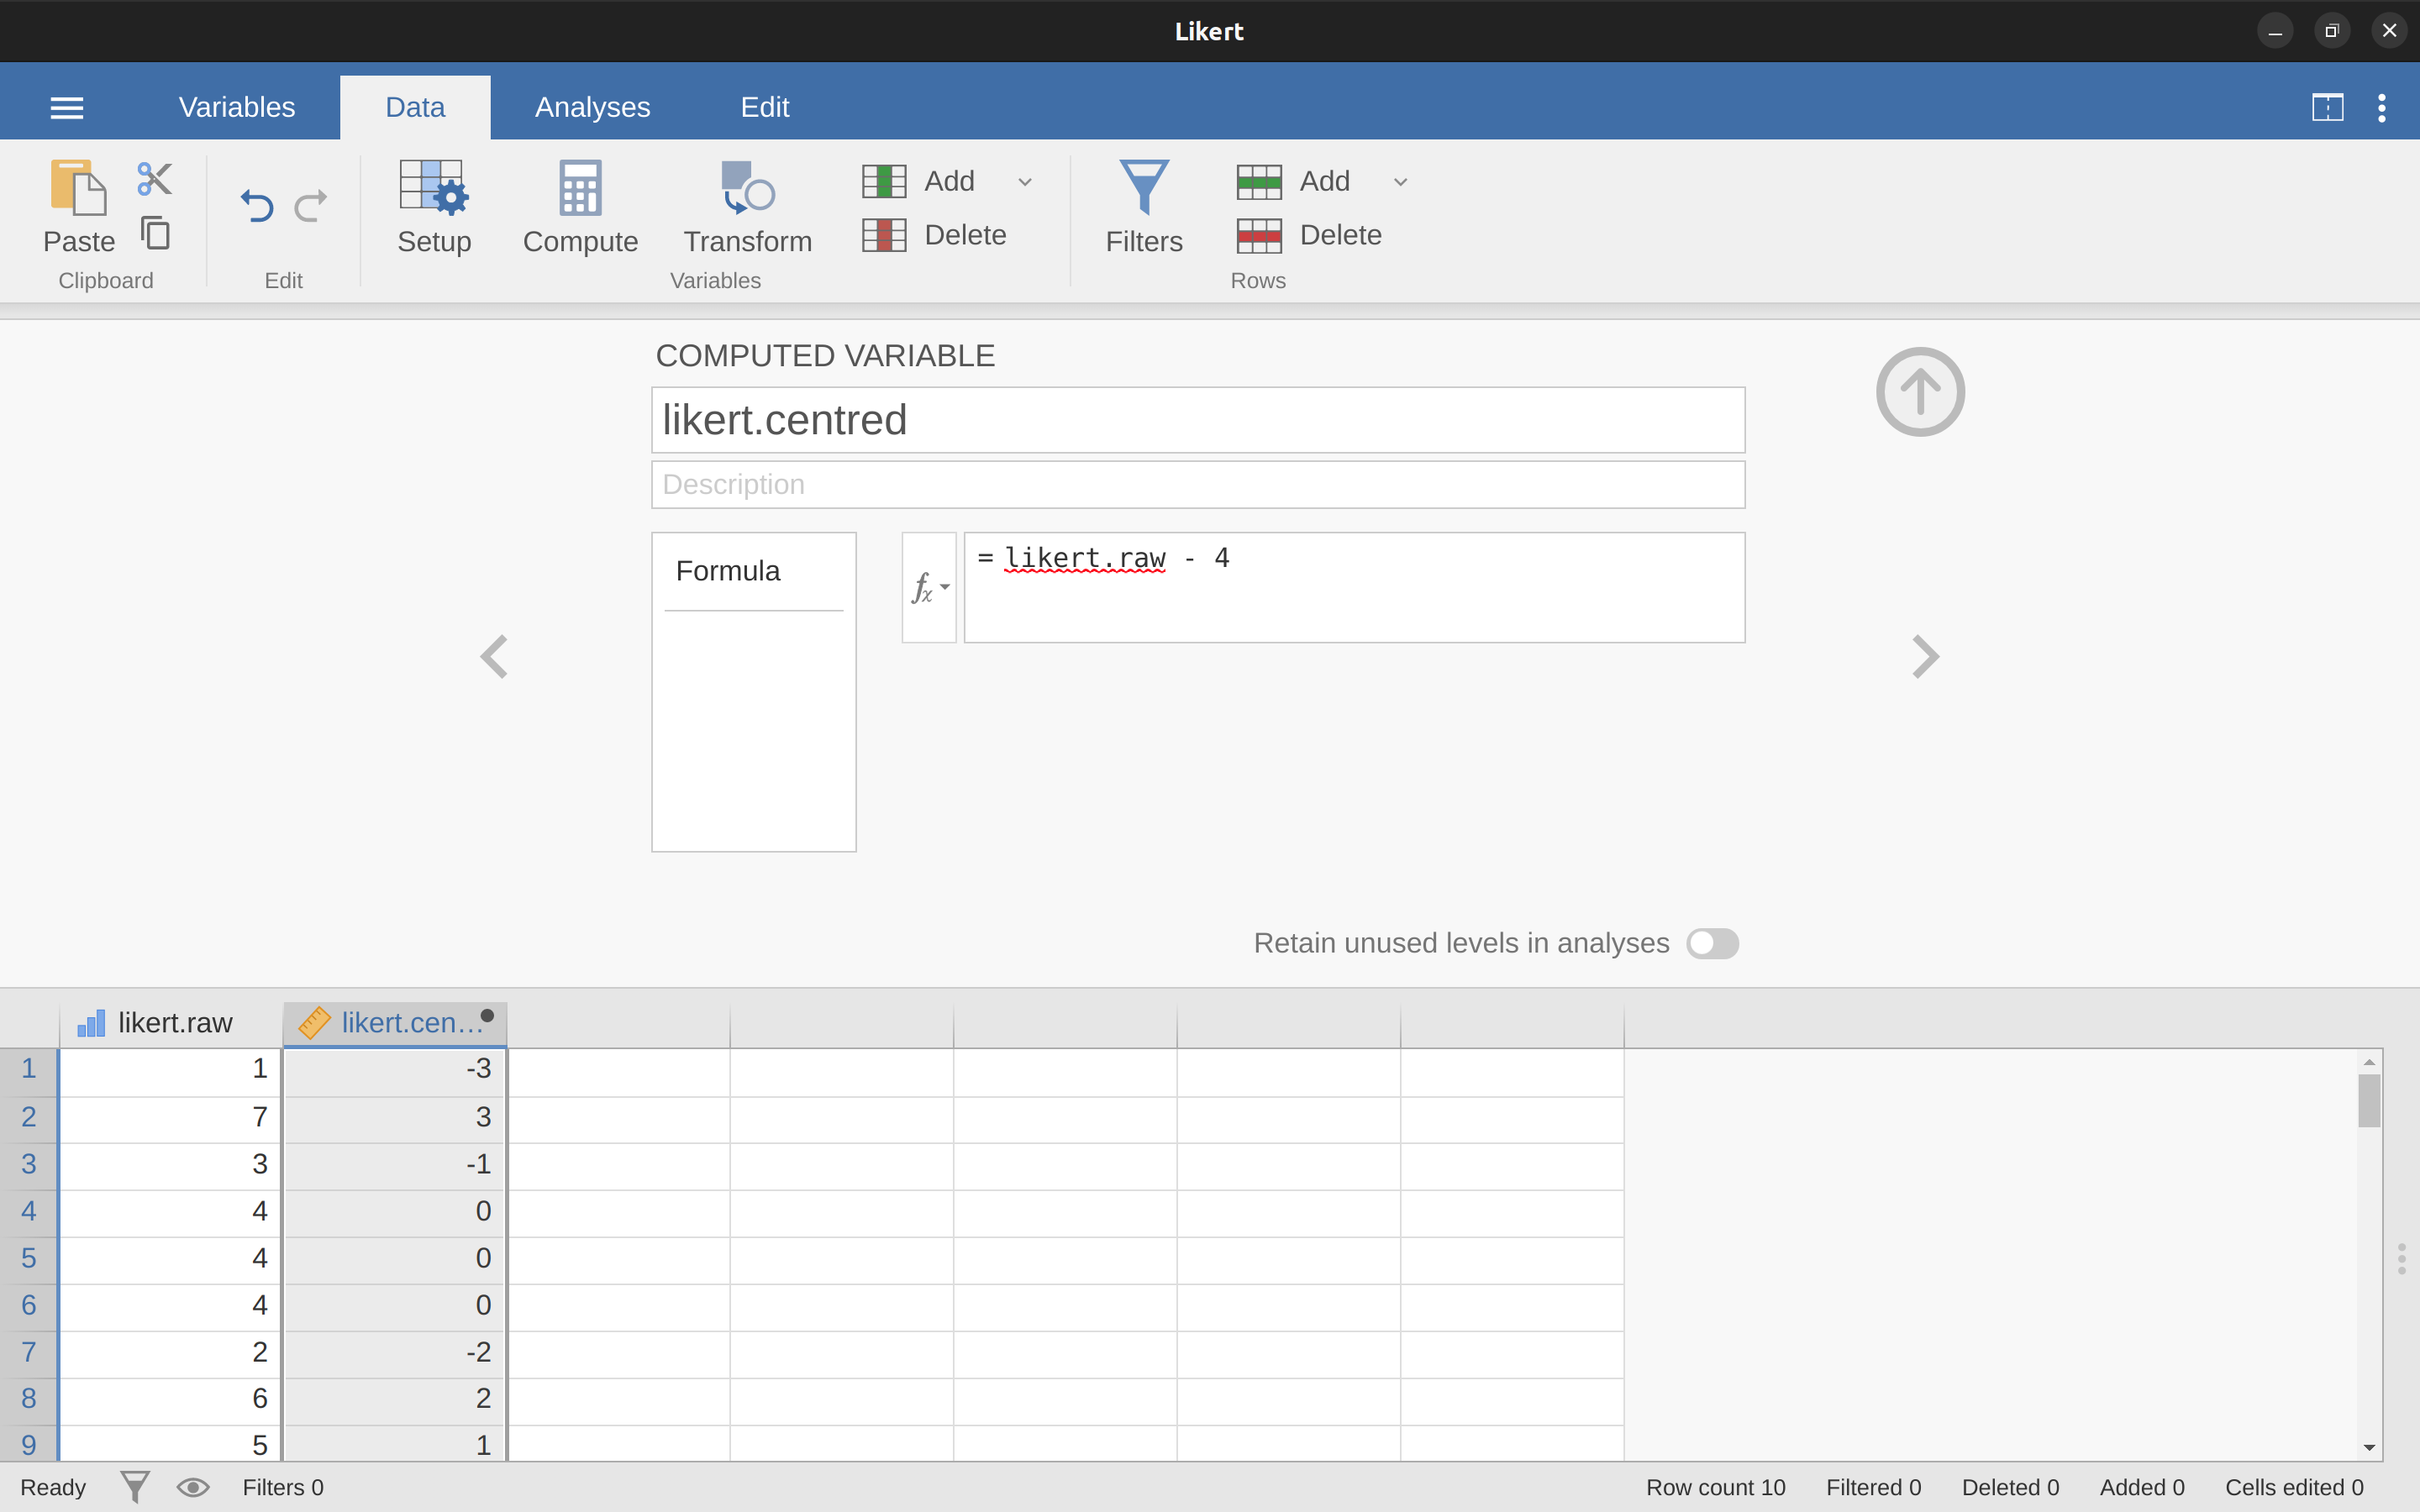
\includegraphics{./images/fig6-4.png} \hfill{}

\caption{\label{fig-fig6-4}Creating a new computed variable in jamovi}

\end{figure}

One reason why it might be useful to have the data in this format is
that there are a lot of situations where you might prefer to analyse the
strength of the opinion separately from the direction of the opinion. We
can do two different transformations on this likert.centred variable in
order to distinguish between these two different concepts. First, to
compute an opinion.strength variable, we want to take the absolute value
of the centred data (using the `ABS' function).\footnote{The absolute
  value of a number is its distance from zero, regardless of whether
  it's sign is negative or positive.} In jamovi, create another new
variable using the `Compute' button. Name the variable opinion.strength
and this time click on the fx button next to the `Formula' box. This
shows the different `Functions' and `Variables' that you can add to the
`Formula' box, so double click on `ABS' and then double click on
``likert.centred' and you will see that the `Formula' box is populated
with ABS(likert.centred) and a new variable has been created in the
spreadsheet view, as in Figure~\ref{fig-fig6-5}.

\begin{figure}

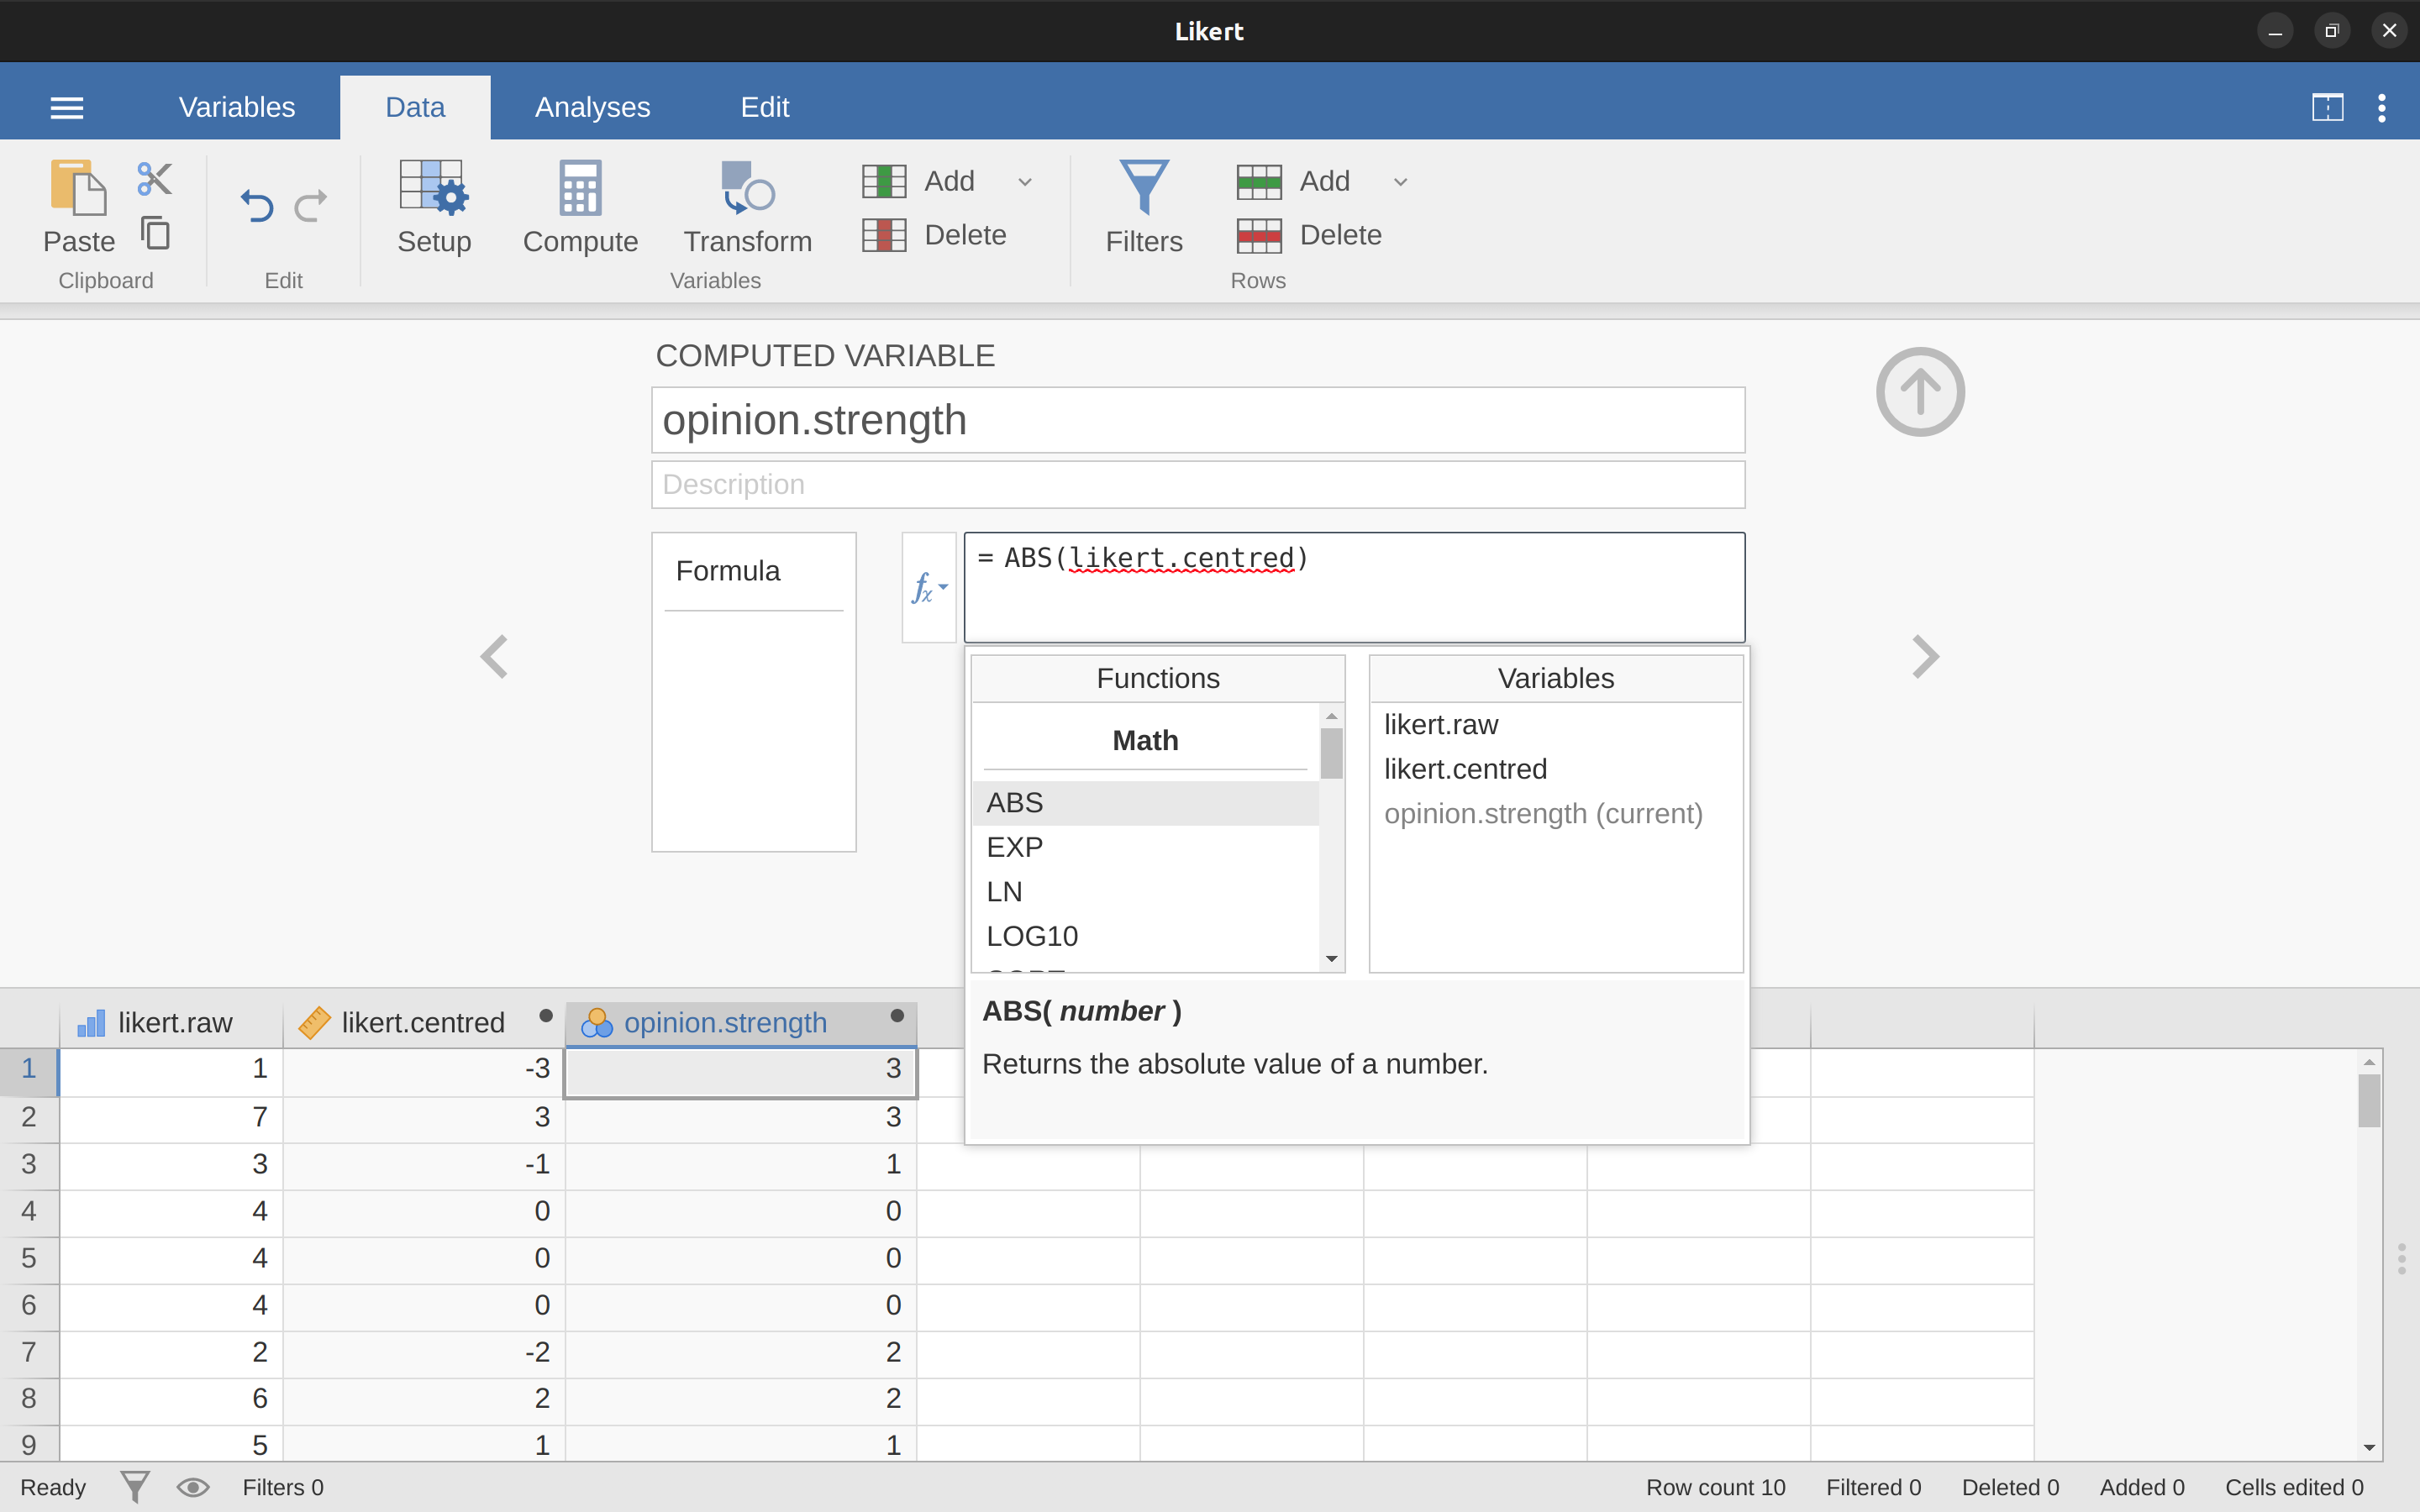
\includegraphics{./images/fig6-5.png} \hfill{}

\caption{\label{fig-fig6-5}Using the \(f_x\) button to select functions
and variables}

\end{figure}

Second, to compute a variable that contains only the direction of the
opinion and ignores the strength, we want to calculate the `sign' of the
variable. In jamovi we can use the IF function to do this. Create
another new variable using the `Compute' button, name this one
opinion.sign, and then type the following into the function box:

IF(likert.centred \(==\) 0, 0, likert.centred / opinion.strength) When
done, you'll see that all negative numbers from the likert.centred
variable are converted to -1, all positive numbers are converted to 1
and zero stays as 0, like so:

-1 1 -1 0 0 0 -1 1 1 1

Let's break down what this `IF' command is doing. In jamovi there are
three parts to an `IF' statement, written as `IF(expression, value,
else)'. The first part, `expression' can be a logical or mathematical
statement. In our example, we have specified `likert.centred \(==\) 0',
which is TRUE for values where likert.centred is zero. The next part,
`value', is the new value where the expression in part one is TRUE. In
our example, we have said that for all those values where likert.centred
is zero, keep them zero. In the next part, `else', we can enter another
logical or mathematical statement to be used if part one evaluates to
FALSE, i.e.~where likert.centred is not zero. In our example we have
divided likert.centred by opinion.strength to give `-1' or `+1'
depending of the sign of the original value in
likert.centred.\footnote{The reason we have to use the `IF' command and
  keep zero as zero is that you cannot just use likert.centred /
  opinion.strength to calculate the sign of likert.centred, because
  mathematically dividing zero by zero does not work. Try it and see}

And we're done. We now have three shiny new variables, all of which are
useful transformations of the original likert.raw data.

\hypertarget{collapsing-a-variable-into-a-smaller-number-of-discrete-levels-or-categories}{%
\subsection{Collapsing a variable into a smaller number of discrete
levels or
categories}\label{collapsing-a-variable-into-a-smaller-number-of-discrete-levels-or-categories}}

One pragmatic task that comes up quite often is the problem of
collapsing a variable into a smaller number of discrete levels or
categories. For instance, suppose I'm interested in looking at the age
distribution of people at a social gathering:

60,58,24,26,34,42,31,30,33,2,9

In some situations it can be quite helpful to group these into a
smallish number of categories. For example, we could group the data into
three broad categories: young (0-20), adult (21-40) and older (41-60).
This is a quite coarse-grained classification, and the labels that I've
attached only make sense in the context of this data set (e.g., viewed
more generally, a 42 year old wouldn't consider themselves as
``older''). We can slice this variable up quite easily using the jamovi
`IF' function that we have already used. This time we have to specify
nested `IF' statements, meaning simply that IF the first logical
expression is TRUE, insert a first value, but IF a second logical
expression is TRUE, insert a second value, but IF a third logical
expression is TRUE, then insert a third value. This can be written as:

IF(Age \textgreater= 0 and Age \textless= 20, 1, IF(Age \textgreater= 21
and Age \textless= 40, 2, IF(Age \textgreater= 41 and Age \textless= 60,
3 )))

Note that there are three left parentheses used during the nesting, so
the whole statement has to end with three right parentheses otherwise
you will get an error message. The jamovi screen shot for this data
manipulation, along with an accompanying frequency table, is shown in
Figure~\ref{fig-fig6-6}.

\begin{figure}

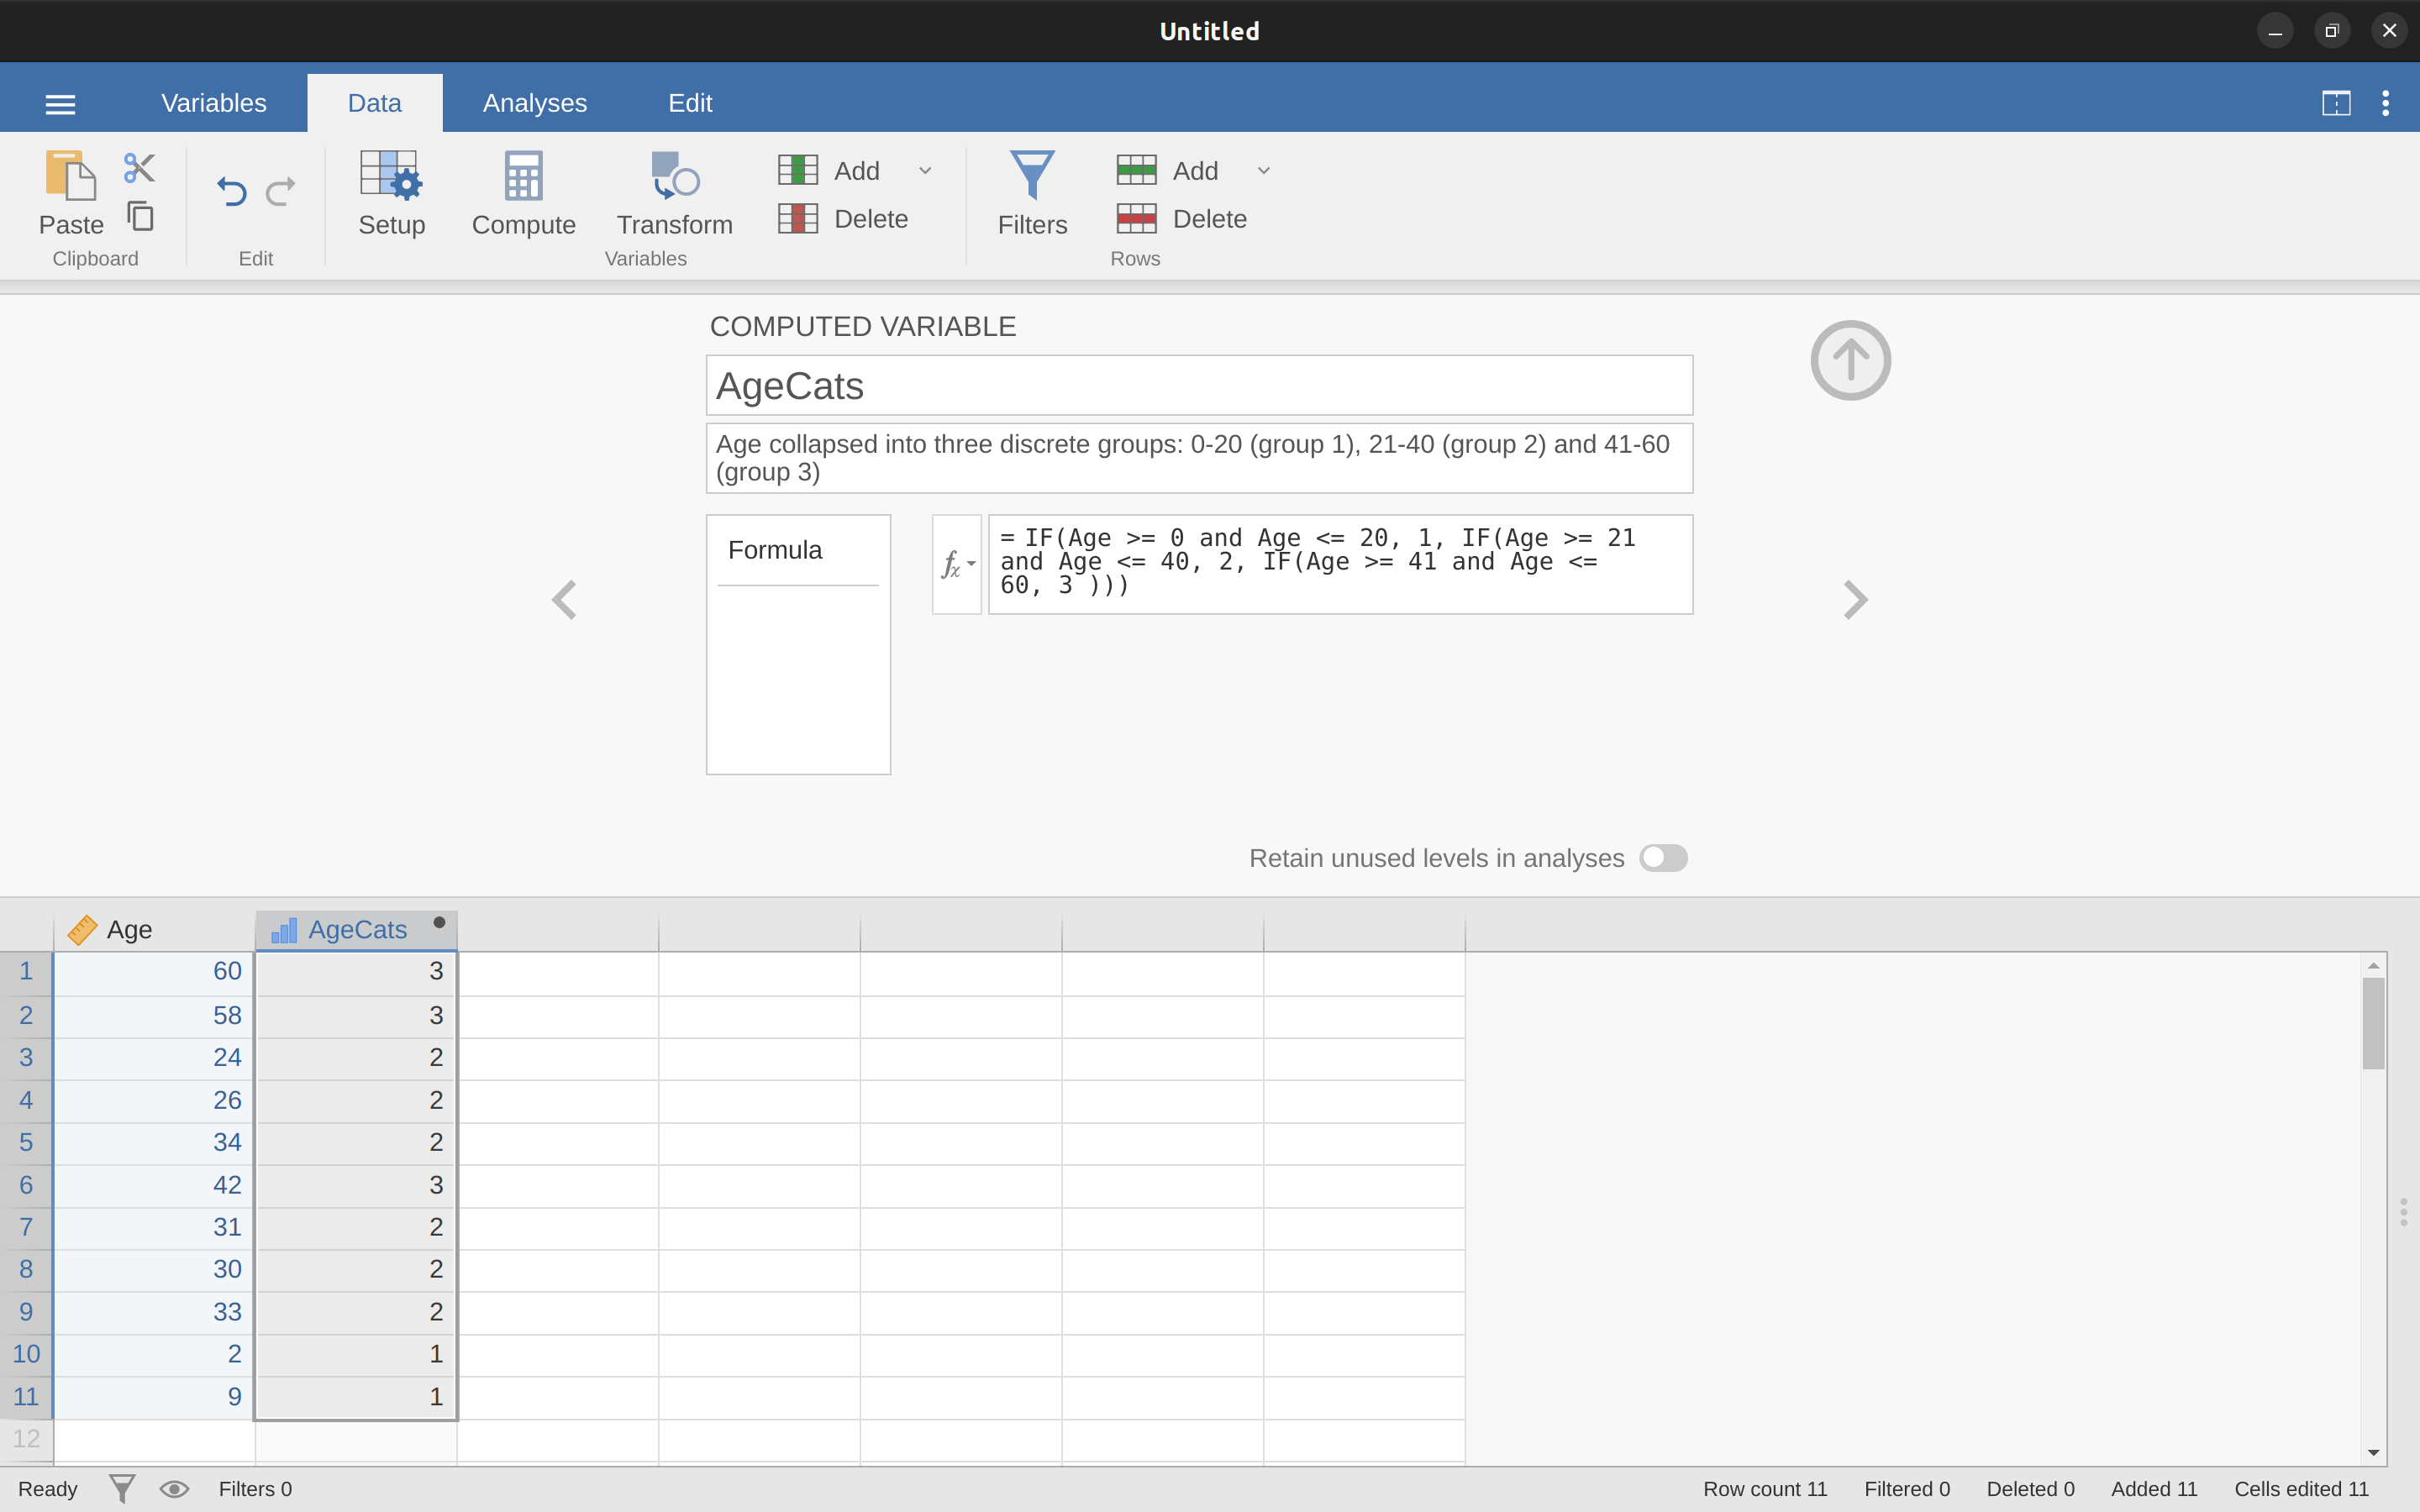
\includegraphics{./images/fig6-6.png} \hfill{}

\caption{\label{fig-fig6-6}Collapsing a variable into a smaller number
of discrete levels using the jamovi `IF' function}

\end{figure}

It's important to take the time to figure out whether or not the
resulting categories make any sense at all in terms of your research
project. If they don't make any sense to you as meaningful categories,
then any data analysis that uses those categories is likely to be just
as meaningless. More generally, in practice I've noticed that people
have a very strong desire to carve their (continuous and messy) data
into a few (discrete and simple) categories, and then run analyses using
the categorised data instead of the original data.\footnote{If you've
  read further into the book, and are re-reading this section, then a
  good example of this would be someone choosing to do an ANOVA using
  AgeCats as the grouping variable, instead of running a regression
  using Age as a predictor. There are sometimes good reasons for doing
  this. For instance, if the relationship between Age and your outcome
  variable is highly non-linear and you aren't comfortable with trying
  to run non-linear regression! However, unless you really do have a
  good rationale for doing this, it's best not to. It tends to introduce
  all sorts of other problems (e.g., the data will probably violate the
  normality assumption) and you can lose a lot of statistical power.} I
wouldn't go so far as to say that this is an inherently bad idea, but it
does have some fairly serious drawbacks at times, so I would advise some
caution if you are thinking about doing it.

\hypertarget{creating-a-transformation-that-can-be-applied-to-multiple-variables}{%
\subsection{Creating a transformation that can be applied to multiple
variables}\label{creating-a-transformation-that-can-be-applied-to-multiple-variables}}

Sometimes you want to apply the same transformation to more than one
variable, for example when you have multiple questionnaire items that
all need to be recalculated or recoded in the same way. And one of the
neat features in jamovi is that you can create a transformation, using
the `Data' - `Transform' button, that can then be saved and applied to
multiple variables. Let's go back to the first example above, using the
data file likert.omv that contains a single variable with raw
Likert-scale responses for 10 people. To create a transformation that
you can save and then apply across multiple variables (assuming you had
more variables like this in your data file), first in the spreadsheet
editor select (i.e., click) the variable you want to use to initially
create the transformation. In our example this is likert.raw. Next click
the `Transform' button in the jamovi `Data' ribbon, and you'll see
something like Figure~\ref{fig-fig6-7}.

Give your new variable a name, let's call it opinion.strength and then
click on the `using transform' selection box and select `Create New
Transform\ldots{}'. This is where you will create, and name, the
transformation that can be re-applied to as many variables as you like.
The transformation is automatically named for us as `Transform 1'
(imaginative, huh. You can change this if you like). Then type the
expression ``ABS(\$source - 4)'' into the function text box, as in
Figure~\ref{fig-fig6-8}, press Enter or Return on your keyboard and, hey
presto, you have created a new transformation and applied it to the
likert.raw variable! Good, eh. Note that instead of using the variable
label in the expression, we have instead used `\$source'. This is so
that we can then use the same transformation with as many different
variables as we like - jamovi requires you to use `\$source' to refer to
the source variable you are transforming. Your transformation has also
been saved and can be re-used any time you like (providing you save the
dataset as an `.omv' file, otherwise you'll lose it!).

You can also create a transformation with the second example we looked
at, the age distribution of people at a social gathering. Go on, you
know you want to! Remember that we collapsed this variable into three
groups: younger, adult and older. This time we will achieve the same
thing, but using the jamovi `Transform' - `Add condition' button. With
this data set (go back to it or create it again if you didn't save it)
set up a new variable transformation. Call the transformed variable
AgeCats and the transformation you will create Agegroupings. Then click
on the big ``\(+\)'' sign next to the function box. This is the `Add
condition' button and I've stuck a big red arrow onto
Figure~\ref{fig-fig6-9} so you can see exactly where this is. Re-create
the transformation shown in Figure~\ref{fig-fig6-9} and when you have
done, you will see the new values appear in the spreadsheet window.
What's more, the Age groupings transformation has been saved and can be
re-applied any time you like. Ok, so I know that it's unlikely you will
have more than one `Age' variable, but you get the idea now of how to
set up transformations in jamovi, so you can follow this idea with other
sorts of variables. A typical scenario for this is when you have a
questionnaire scale with, say, 20 items (variables) and each item was
originally scored from 1 to 6 but, for some reason or quirk of the data
you decide to recode all the items as 1 to 3. You can easily do this in
jamovi by creating and then re-applying your transformation for each
variable that you want to recode.

\begin{figure}

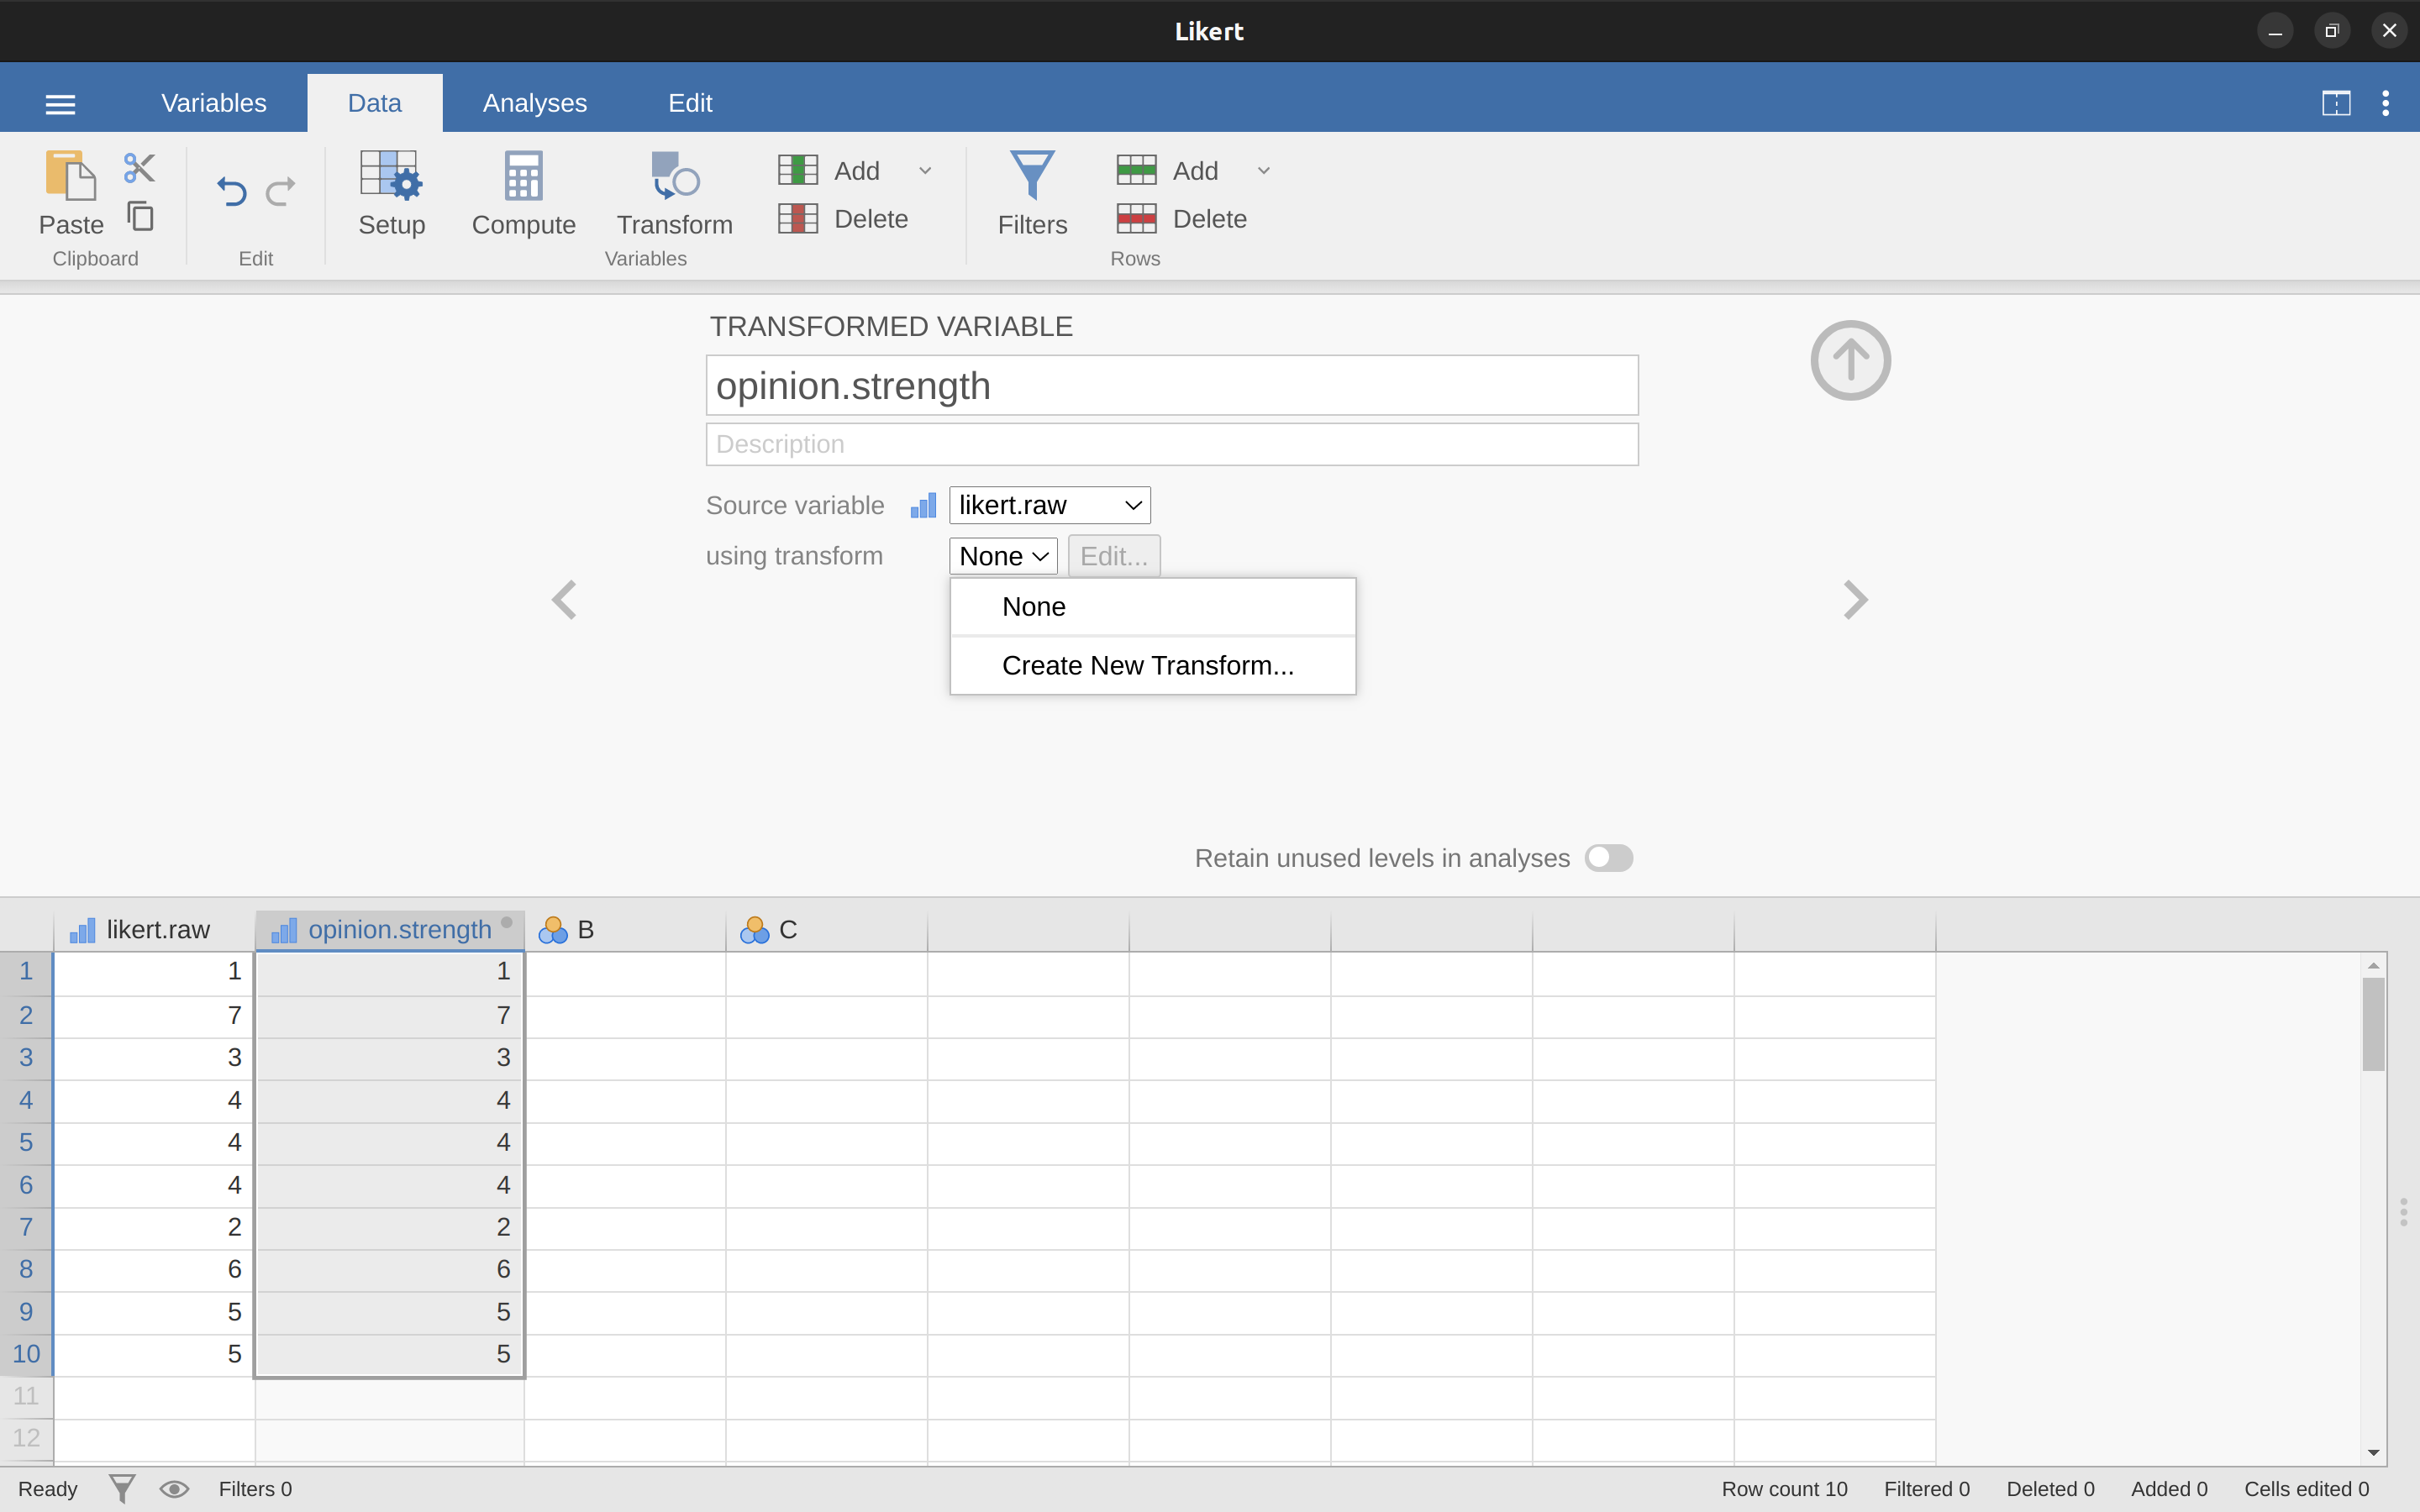
\includegraphics{./images/fig6-7.png} \hfill{}

\caption{\label{fig-fig6-7}Creating a new variable transformation using
the jamovi `Transform' command}

\end{figure}

\begin{figure}

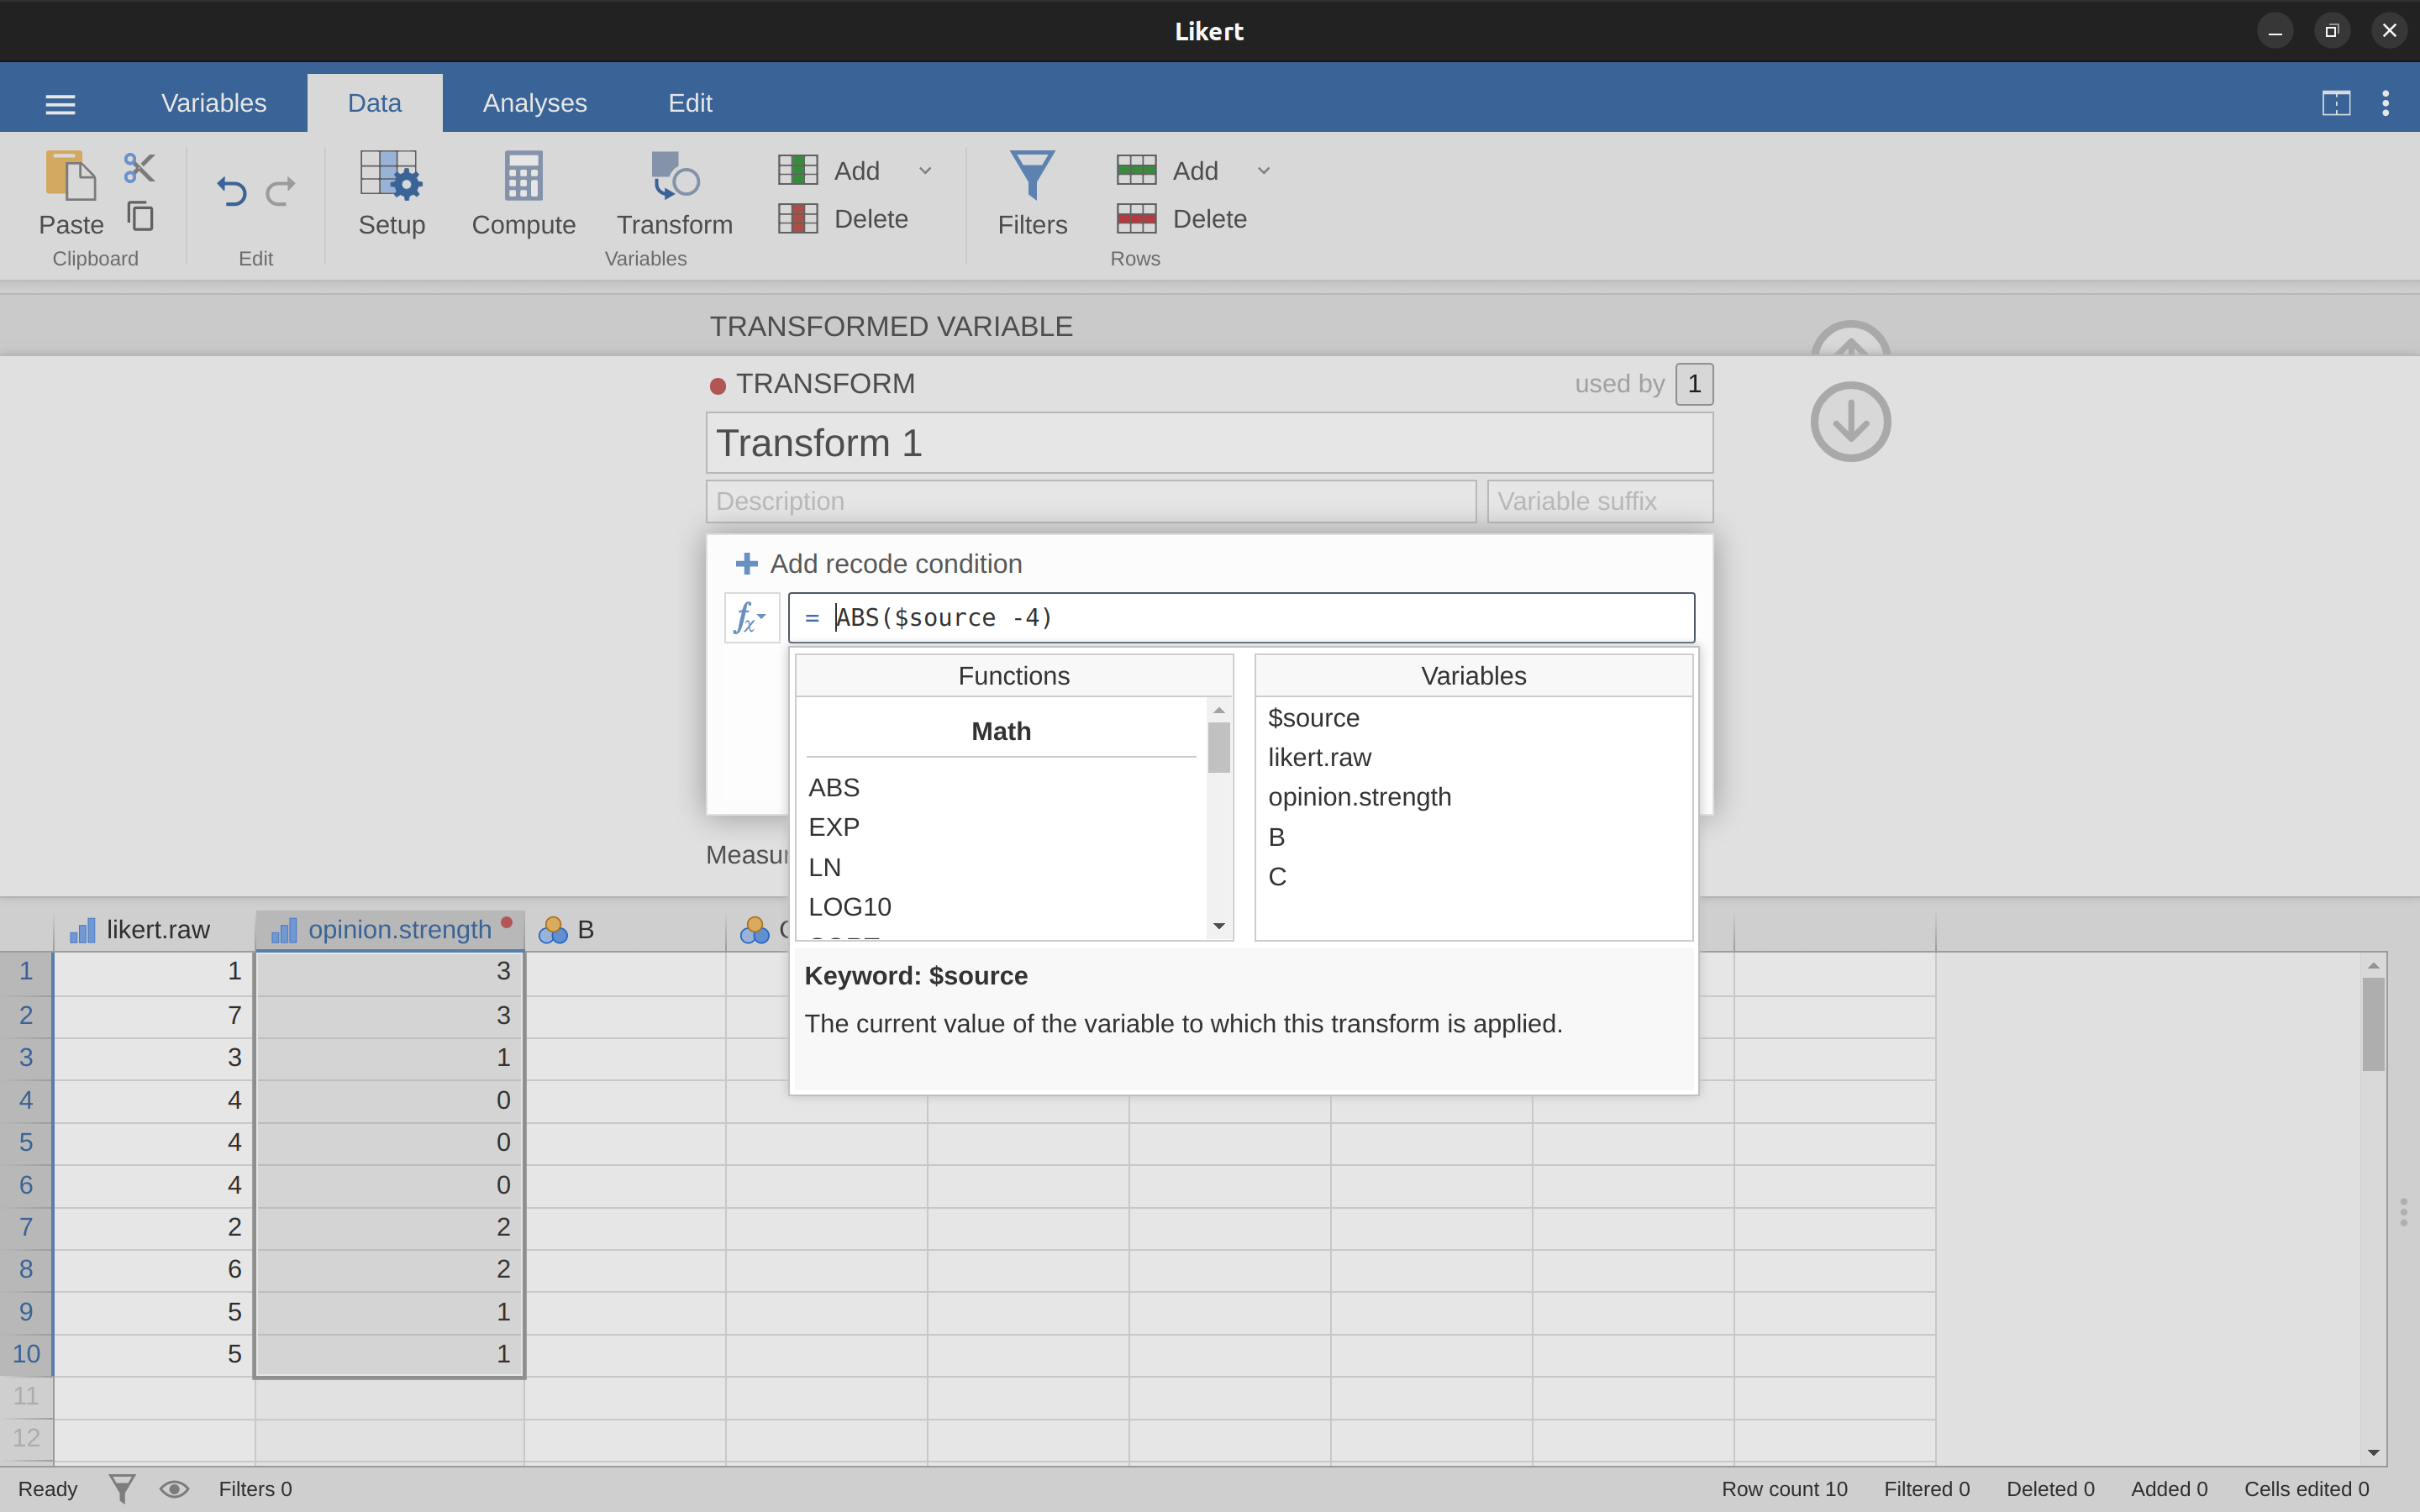
\includegraphics{./images/fig6-8.png} \hfill{}

\caption{\label{fig-fig6-8}Specifying a transformation in jamovi, to be
saved as the imaginatively named `Transform 1'}

\end{figure}

\begin{figure}

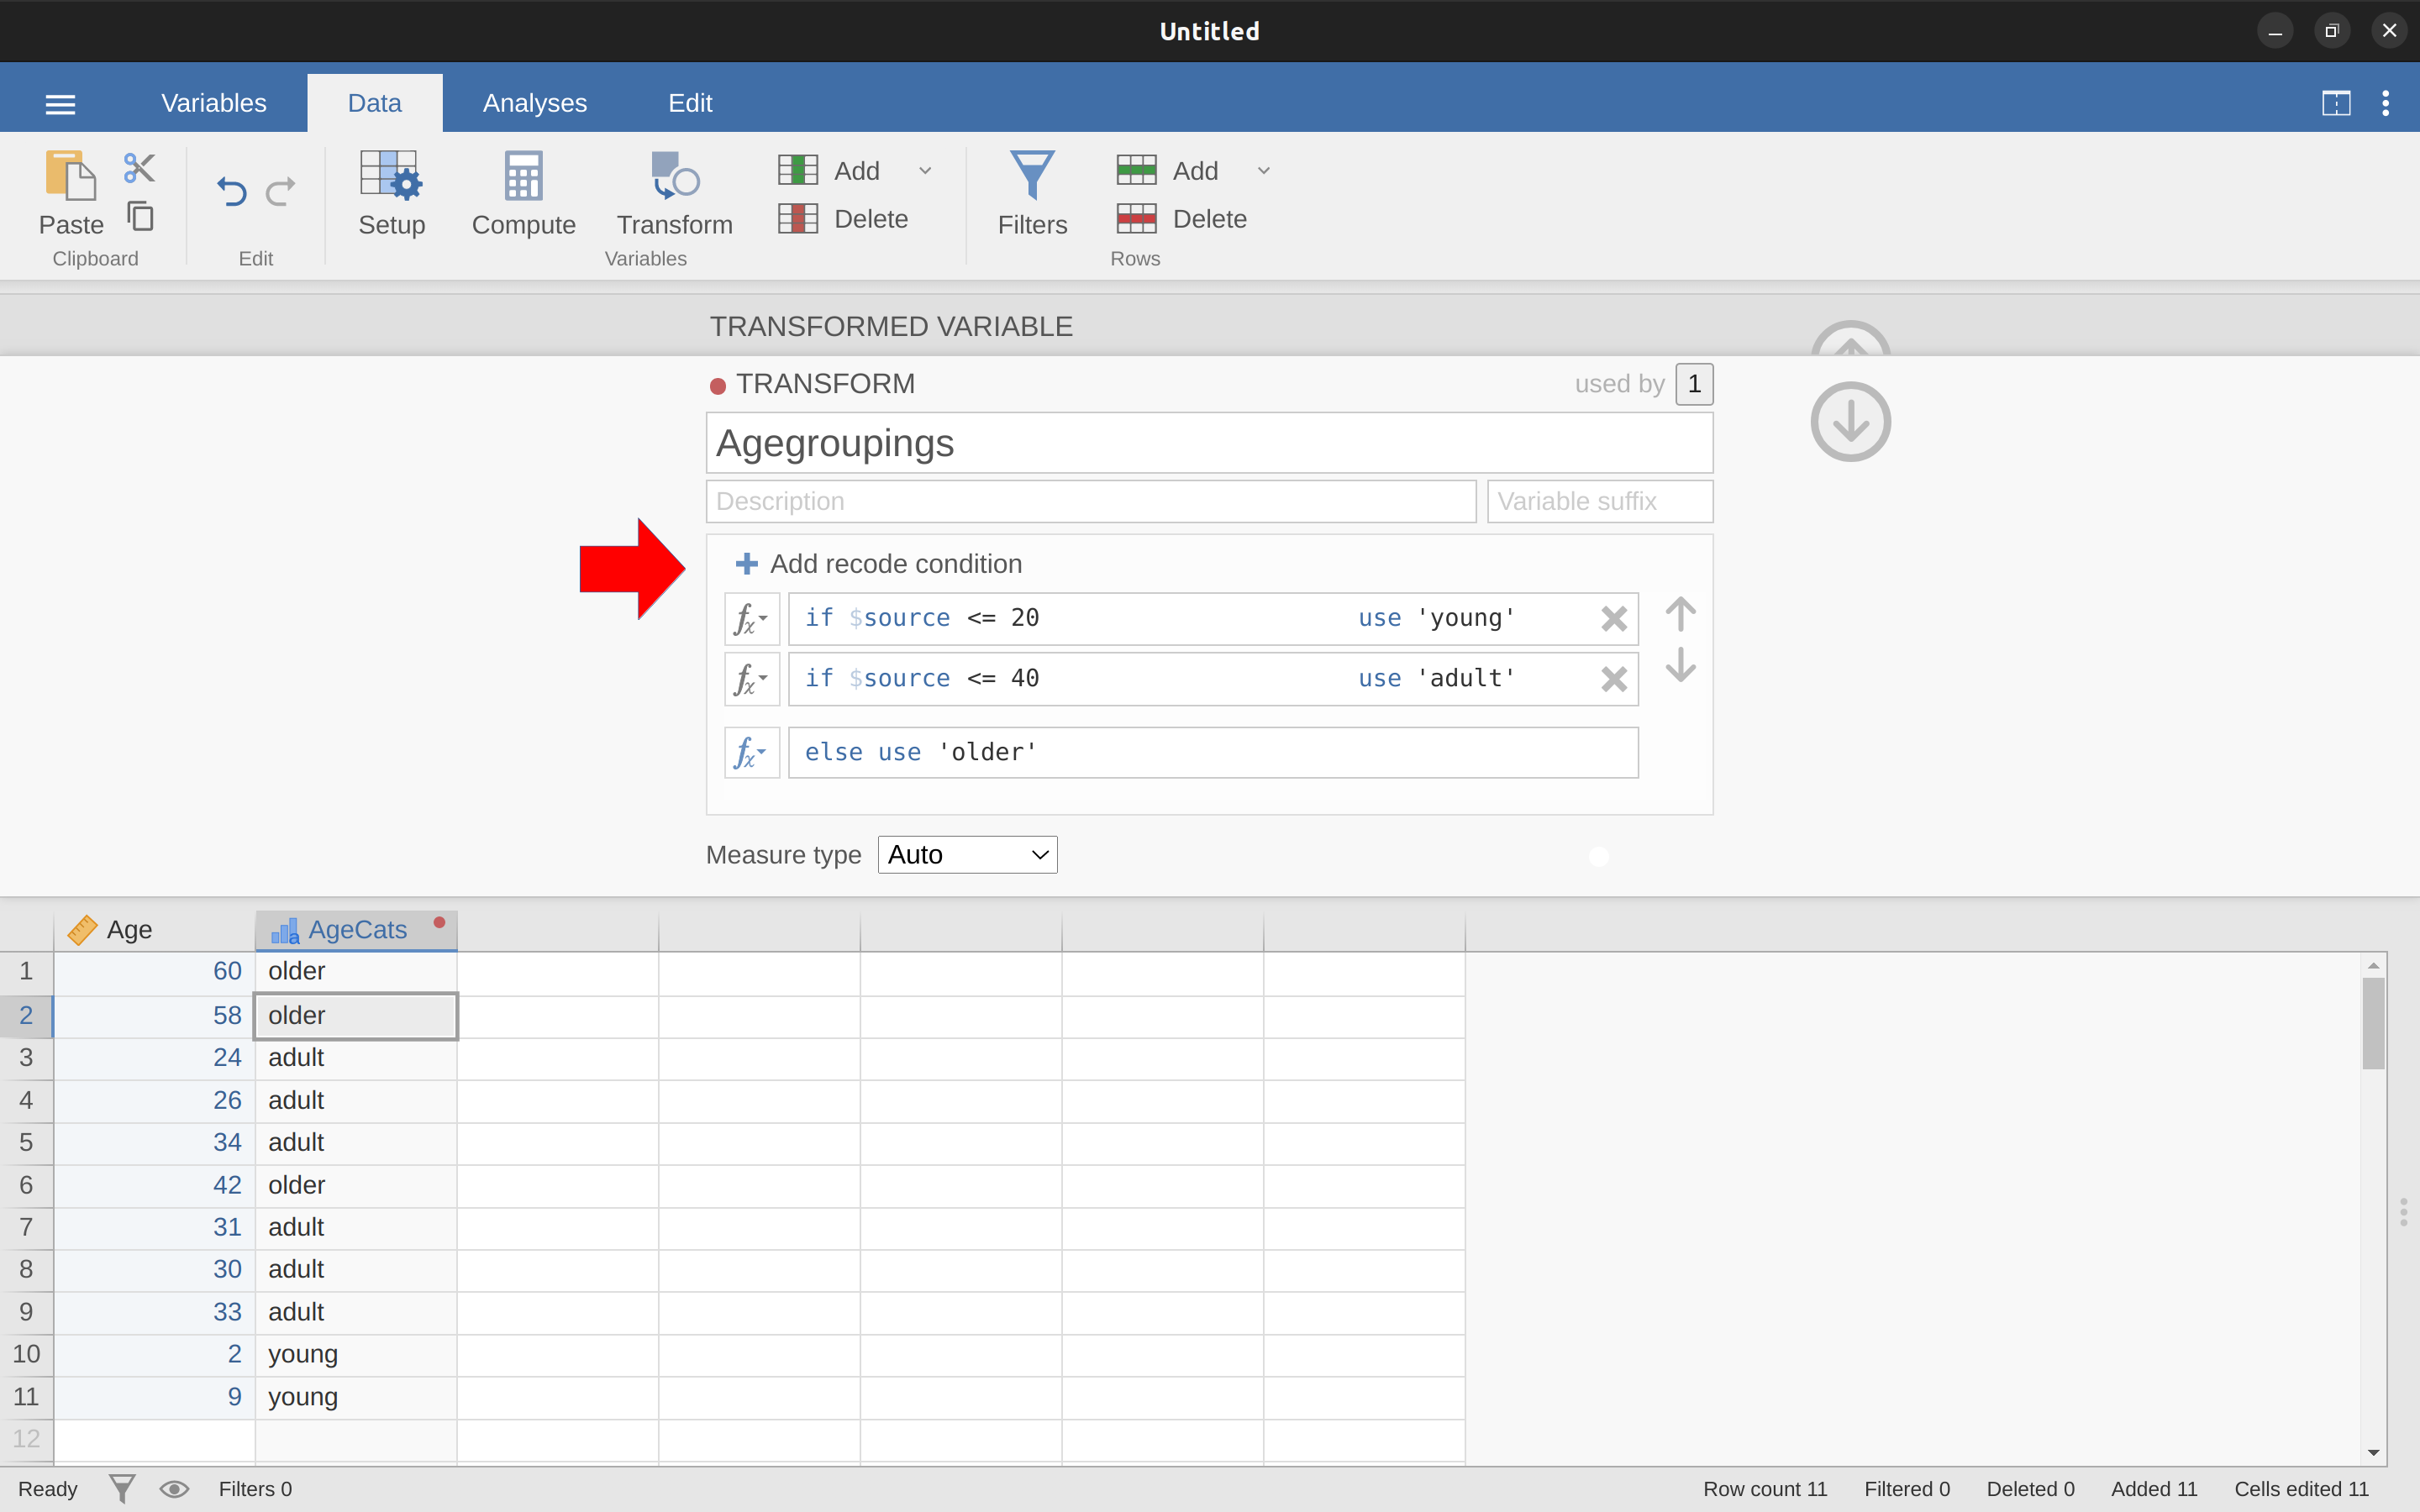
\includegraphics{./images/fig6-9.png} \hfill{}

\caption{\label{fig-fig6-9}jamovi transformation into three age
categories, using the `Add condition' button}

\end{figure}

\hypertarget{tbl-tab6-5}{}
 
  \providecommand{\huxb}[2]{\arrayrulecolor[RGB]{#1}\global\arrayrulewidth=#2pt}
  \providecommand{\huxvb}[2]{\color[RGB]{#1}\vrule width #2pt}
  \providecommand{\huxtpad}[1]{\rule{0pt}{#1}}
  \providecommand{\huxbpad}[1]{\rule[-#1]{0pt}{#1}}

\begin{table}[ht]
\caption{\label{tbl-tab6-5}Some mathematical operators }\tabularnewline

\begin{centerbox}
\begin{threeparttable}
\setlength{\tabcolsep}{0pt}
\begin{tabularx}{0.9\textwidth}{p{0.225\textwidth} p{0.225\textwidth} p{0.225\textwidth} p{0.225\textwidth}}


\hhline{>{\huxb{0, 0, 0}{0.4}}->{\huxb{0, 0, 0}{0.4}}->{\huxb{0, 0, 0}{0.4}}->{\huxb{0, 0, 0}{0.4}}-}
\arrayrulecolor{black}

\multicolumn{1}{!{\huxvb{0, 0, 0}{0}}p{0.225\textwidth}!{\huxvb{0, 0, 0}{0}}}{\cellcolor[RGB]{242, 242, 242}\hspace{0pt}\parbox[b]{0.225\textwidth-0pt-6pt}{\huxtpad{6pt + 1em}\centering \textbf{}\huxbpad{6pt}}} &
\multicolumn{1}{p{0.225\textwidth}!{\huxvb{0, 0, 0}{0}}}{\cellcolor[RGB]{242, 242, 242}\hspace{6pt}\parbox[b]{0.225\textwidth-6pt-6pt}{\huxtpad{6pt + 1em}\centering \textbf{function}\huxbpad{6pt}}} &
\multicolumn{1}{p{0.225\textwidth}!{\huxvb{0, 0, 0}{0}}}{\cellcolor[RGB]{242, 242, 242}\hspace{6pt}\parbox[b]{0.225\textwidth-6pt-6pt}{\huxtpad{6pt + 1em}\centering \textbf{example input}\huxbpad{6pt}}} &
\multicolumn{1}{p{0.225\textwidth}!{\huxvb{0, 0, 0}{0}}}{\cellcolor[RGB]{242, 242, 242}\hspace{6pt}\parbox[b]{0.225\textwidth-6pt-0pt}{\huxtpad{6pt + 1em}\centering \textbf{(answer)}\huxbpad{6pt}}} \tabularnewline[-0.5pt]


\hhline{>{\huxb{0, 0, 0}{0.4}}->{\huxb{0, 0, 0}{0.4}}->{\huxb{0, 0, 0}{0.4}}->{\huxb{0, 0, 0}{0.4}}-}
\arrayrulecolor{black}

\multicolumn{1}{!{\huxvb{0, 0, 0}{0}}p{0.225\textwidth}!{\huxvb{0, 0, 0}{0}}}{\hspace{0pt}\parbox[b]{0.225\textwidth-0pt-6pt}{\huxtpad{6pt + 1em}\centering square root\huxbpad{6pt}}} &
\multicolumn{1}{p{0.225\textwidth}!{\huxvb{0, 0, 0}{0}}}{\hspace{6pt}\parbox[b]{0.225\textwidth-6pt-6pt}{\huxtpad{6pt + 1em}\centering SQRT(x)\huxbpad{6pt}}} &
\multicolumn{1}{p{0.225\textwidth}!{\huxvb{0, 0, 0}{0}}}{\hspace{6pt}\parbox[b]{0.225\textwidth-6pt-6pt}{\huxtpad{6pt + 1em}\centering SQRT(25)\huxbpad{6pt}}} &
\multicolumn{1}{p{0.225\textwidth}!{\huxvb{0, 0, 0}{0}}}{\hspace{6pt}\parbox[b]{0.225\textwidth-6pt-0pt}{\huxtpad{6pt + 1em}\centering 5\huxbpad{6pt}}} \tabularnewline[-0.5pt]


\hhline{}
\arrayrulecolor{black}

\multicolumn{1}{!{\huxvb{0, 0, 0}{0}}p{0.225\textwidth}!{\huxvb{0, 0, 0}{0}}}{\cellcolor[RGB]{242, 242, 242}\hspace{0pt}\parbox[b]{0.225\textwidth-0pt-6pt}{\huxtpad{6pt + 1em}\centering absolute value\huxbpad{6pt}}} &
\multicolumn{1}{p{0.225\textwidth}!{\huxvb{0, 0, 0}{0}}}{\cellcolor[RGB]{242, 242, 242}\hspace{6pt}\parbox[b]{0.225\textwidth-6pt-6pt}{\huxtpad{6pt + 1em}\centering ABS(x)\huxbpad{6pt}}} &
\multicolumn{1}{p{0.225\textwidth}!{\huxvb{0, 0, 0}{0}}}{\cellcolor[RGB]{242, 242, 242}\hspace{6pt}\parbox[b]{0.225\textwidth-6pt-6pt}{\huxtpad{6pt + 1em}\centering ABS(-23)\huxbpad{6pt}}} &
\multicolumn{1}{p{0.225\textwidth}!{\huxvb{0, 0, 0}{0}}}{\cellcolor[RGB]{242, 242, 242}\hspace{6pt}\parbox[b]{0.225\textwidth-6pt-0pt}{\huxtpad{6pt + 1em}\centering 23\huxbpad{6pt}}} \tabularnewline[-0.5pt]


\hhline{}
\arrayrulecolor{black}

\multicolumn{1}{!{\huxvb{0, 0, 0}{0}}p{0.225\textwidth}!{\huxvb{0, 0, 0}{0}}}{\hspace{0pt}\parbox[b]{0.225\textwidth-0pt-6pt}{\huxtpad{6pt + 1em}\centering logarithm (base 10)\huxbpad{6pt}}} &
\multicolumn{1}{p{0.225\textwidth}!{\huxvb{0, 0, 0}{0}}}{\hspace{6pt}\parbox[b]{0.225\textwidth-6pt-6pt}{\huxtpad{6pt + 1em}\centering LOG10(x)\huxbpad{6pt}}} &
\multicolumn{1}{p{0.225\textwidth}!{\huxvb{0, 0, 0}{0}}}{\hspace{6pt}\parbox[b]{0.225\textwidth-6pt-6pt}{\huxtpad{6pt + 1em}\centering LOG10(1000)\huxbpad{6pt}}} &
\multicolumn{1}{p{0.225\textwidth}!{\huxvb{0, 0, 0}{0}}}{\hspace{6pt}\parbox[b]{0.225\textwidth-6pt-0pt}{\huxtpad{6pt + 1em}\centering 3\huxbpad{6pt}}} \tabularnewline[-0.5pt]


\hhline{}
\arrayrulecolor{black}

\multicolumn{1}{!{\huxvb{0, 0, 0}{0}}p{0.225\textwidth}!{\huxvb{0, 0, 0}{0}}}{\cellcolor[RGB]{242, 242, 242}\hspace{0pt}\parbox[b]{0.225\textwidth-0pt-6pt}{\huxtpad{6pt + 1em}\centering logarithm (base e)\huxbpad{6pt}}} &
\multicolumn{1}{p{0.225\textwidth}!{\huxvb{0, 0, 0}{0}}}{\cellcolor[RGB]{242, 242, 242}\hspace{6pt}\parbox[b]{0.225\textwidth-6pt-6pt}{\huxtpad{6pt + 1em}\centering LN(x)\huxbpad{6pt}}} &
\multicolumn{1}{p{0.225\textwidth}!{\huxvb{0, 0, 0}{0}}}{\cellcolor[RGB]{242, 242, 242}\hspace{6pt}\parbox[b]{0.225\textwidth-6pt-6pt}{\huxtpad{6pt + 1em}\centering LN(1000)\huxbpad{6pt}}} &
\multicolumn{1}{p{0.225\textwidth}!{\huxvb{0, 0, 0}{0}}}{\cellcolor[RGB]{242, 242, 242}\hspace{6pt}\parbox[b]{0.225\textwidth-6pt-0pt}{\huxtpad{6pt + 1em}\centering 6.91\huxbpad{6pt}}} \tabularnewline[-0.5pt]


\hhline{}
\arrayrulecolor{black}

\multicolumn{1}{!{\huxvb{0, 0, 0}{0}}p{0.225\textwidth}!{\huxvb{0, 0, 0}{0}}}{\hspace{0pt}\parbox[b]{0.225\textwidth-0pt-6pt}{\huxtpad{6pt + 1em}\centering exponentiation\huxbpad{6pt}}} &
\multicolumn{1}{p{0.225\textwidth}!{\huxvb{0, 0, 0}{0}}}{\hspace{6pt}\parbox[b]{0.225\textwidth-6pt-6pt}{\huxtpad{6pt + 1em}\centering EXP(x)\huxbpad{6pt}}} &
\multicolumn{1}{p{0.225\textwidth}!{\huxvb{0, 0, 0}{0}}}{\hspace{6pt}\parbox[b]{0.225\textwidth-6pt-6pt}{\huxtpad{6pt + 1em}\centering EXP(6.908)\huxbpad{6pt}}} &
\multicolumn{1}{p{0.225\textwidth}!{\huxvb{0, 0, 0}{0}}}{\hspace{6pt}\parbox[b]{0.225\textwidth-6pt-0pt}{\huxtpad{6pt + 1em}\centering 1e+03\huxbpad{6pt}}} \tabularnewline[-0.5pt]


\hhline{}
\arrayrulecolor{black}

\multicolumn{1}{!{\huxvb{0, 0, 0}{0}}p{0.225\textwidth}!{\huxvb{0, 0, 0}{0}}}{\cellcolor[RGB]{242, 242, 242}\hspace{0pt}\parbox[b]{0.225\textwidth-0pt-6pt}{\huxtpad{6pt + 1em}\centering box-cox\huxbpad{6pt}}} &
\multicolumn{1}{p{0.225\textwidth}!{\huxvb{0, 0, 0}{0}}}{\cellcolor[RGB]{242, 242, 242}\hspace{6pt}\parbox[b]{0.225\textwidth-6pt-6pt}{\huxtpad{6pt + 1em}\centering BOXCOX(x, lamda)\huxbpad{6pt}}} &
\multicolumn{1}{p{0.225\textwidth}!{\huxvb{0, 0, 0}{0}}}{\cellcolor[RGB]{242, 242, 242}\hspace{6pt}\parbox[b]{0.225\textwidth-6pt-6pt}{\huxtpad{6pt + 1em}\centering BOXCOX(6.908, 3)\huxbpad{6pt}}} &
\multicolumn{1}{p{0.225\textwidth}!{\huxvb{0, 0, 0}{0}}}{\cellcolor[RGB]{242, 242, 242}\hspace{6pt}\parbox[b]{0.225\textwidth-6pt-0pt}{\huxtpad{6pt + 1em}\centering 110\huxbpad{6pt}}} \tabularnewline[-0.5pt]


\hhline{>{\huxb{0, 0, 0}{0.4}}->{\huxb{0, 0, 0}{0.4}}->{\huxb{0, 0, 0}{0.4}}->{\huxb{0, 0, 0}{0.4}}-}
\arrayrulecolor{black}
\end{tabularx} 

\end{threeparttable}\par\end{centerbox}

\end{table}
 

\hypertarget{a-few-more-mathematical-functions-and-operations}{%
\section{A few more mathematical functions and
operations}\label{a-few-more-mathematical-functions-and-operations}}

In the section on
\protect\hyperlink{sec-Transforming-and-recoding-a-variable}{Transforming
and recoding a variable} I discussed the ideas behind variable
transformations and showed that a lot of the transformations that you
might want to apply to your data are based on fairly simple mathematical
functions and operations. In this section I want to return to that
discussion and mention several other mathematical functions and
arithmetic operations that are actually quite useful for a lot of real
world data analysis. Table~\ref{tbl-tab6-5} gives a brief overview of
the various mathematical functions I want to talk about here, or
later.\footnote{We'll leave the box-cox function until later on}
Obviously this doesn't even come close to cataloguing the range of
possibilities available, but it does cover a range of functions that are
used regularly in data analysis and that are available in jamovi.

\hypertarget{logarithms-and-exponentials}{%
\subsection{Logarithms and
exponentials}\label{logarithms-and-exponentials}}

As I've mentioned earlier, jamovi has an useful range of mathematical
functions built into it and there really wouldn't be much point in
trying to describe or even list all of them. For the most part, I've
focused only on those functions that are strictly necessary for this
book. However I do want to make an exception for logarithms and
exponentials. Although they aren't needed anywhere else in this book,
they are \emph{everywhere} in statistics more broadly. And not only
that, there are a \emph{lot of} situations in which it is convenient to
analyse the logarithm of a variable (i.e., to take a ``log-transform''
of the variable). I suspect that many (maybe most) readers of this book
will have encountered logarithms and exponentials before, but from past
experience I know that there's a substantial proportion of students who
take a social science statistics class who haven't touched logarithms
since high school, and would appreciate a bit of a refresher.

In order to understand logarithms and exponentials, the easiest thing to
do is to actually calculate them and see how they relate to other simple
calculations. There are three jamovi functions in particular that I want
to talk about, namely LN(), LOG10() and EXP(). To start with, let's
consider LOG10(), which is known as the ``logarithm in base 10''. The
trick to understanding a \textbf{logarithm} is to understand that it's
basically the ``opposite'' of taking a power. Specifically, the
logarithm in base 10 is closely related to the powers of 10. So let's
start by noting that 10-cubed is 1000. Mathematically, we would write
this:

\[10^3=1000\]

The trick to understanding a logarithm is to recognise that the
statement that ``10 to the power of 3 is equal to 1000'' is equivalent
to the statement that ``the logarithm (in base 10) of 1000 is equal to
3''. Mathematically, we write this as follows,

\[log_{10}(1000)=3\]

Okay, since the LOG10() function is related to the powers of 10, you
might expect that there are other logarithms (in bases other than 10)
that are related to other powers too. And of course that's true: there's
not really anything mathematically special about the number 10. You and
I happen to find it useful because decimal numbers are built around the
number 10, but the big bad world of mathematics scoffs at our decimal
numbers. Sadly, the universe doesn't actually care how we write down
numbers. Anyway, the consequence of this cosmic indifference is that
there's nothing particularly special about calculating logarithms in
base 10. You could, for instance, calculate your logarithms in base 2.
Alternatively, a third type of logarithm, and one we see a lot more of
in statistics than either base 10 or base 2, is called the
\textbf{natural logarithm}, and corresponds to the logarithm in base e.
Since you might one day run into it, I'd better explain what e is. The
number e, known as \textbf{Euler's number}, is one of those annoying
``irrational'' numbers whose decimal expansion is infinitely long, and
is considered one of the most important numbers in mathematics. The
first few digits of e are:

\[e = 2.718282 \]

There are quite a few situation in statistics that require us to
calculate powers of \(e\), though none of them appear in this book.
Raising e to the power \(x\) is called the \textbf{exponential} of
\(x\), and so it's very common to see \(e^x\) written as exppxq. And so
it's no surprise that jamovi has a function that calculates
exponentials, called EXP(). Because the number e crops up so often in
statistics, the natural logarithm (i.e., logarithm in base e) also tends
to turn up. Mathematicians often write it as \(log_e(x)\) or \(ln(x)\).
In fact, jamovi works the same way: the LN() function corresponds to the
natural logarithm.

And with that, I think we've had quite enough exponentials and
logarithms for this book!

\hypertarget{extracting-a-subset-of-the-data}{%
\section{Extracting a subset of the
data}\label{extracting-a-subset-of-the-data}}

One very important kind of data handling is being able to extract a
particular subset of the data. For instance, you might be interested
only in analysing the data from one experimental condition, or you may
want to look closely at the data from people over 50 years in age. To do
this, the first step is getting jamovi to filter the subset of the data
corresponding to the observations that you're interested in.

This section returns to the nightgarden.csv data set. If you're reading
this whole chapter in one sitting, then you should already have this
data set loaded into a jamovi window. For this section, let's focus on
the two variables speaker and utterance (see
\protect\hyperlink{sec-Tabulating-and-cross-tabulating-data}{Tabulating
and cross-tabulating data}) if you've forgotten what those variables
look like). Suppose that what I want to do is pull out only those
utterances that were made by Makka-Pakka. To that end, we need to
specify a filter in jamovi. First open up a filter window by clicking on
`Filters' on the main jamovi `Data' toolbar. Then, in the `Filter 1'
text box, next to the `=' sign, type the following:

speaker == `makka-pakka'

\begin{figure}

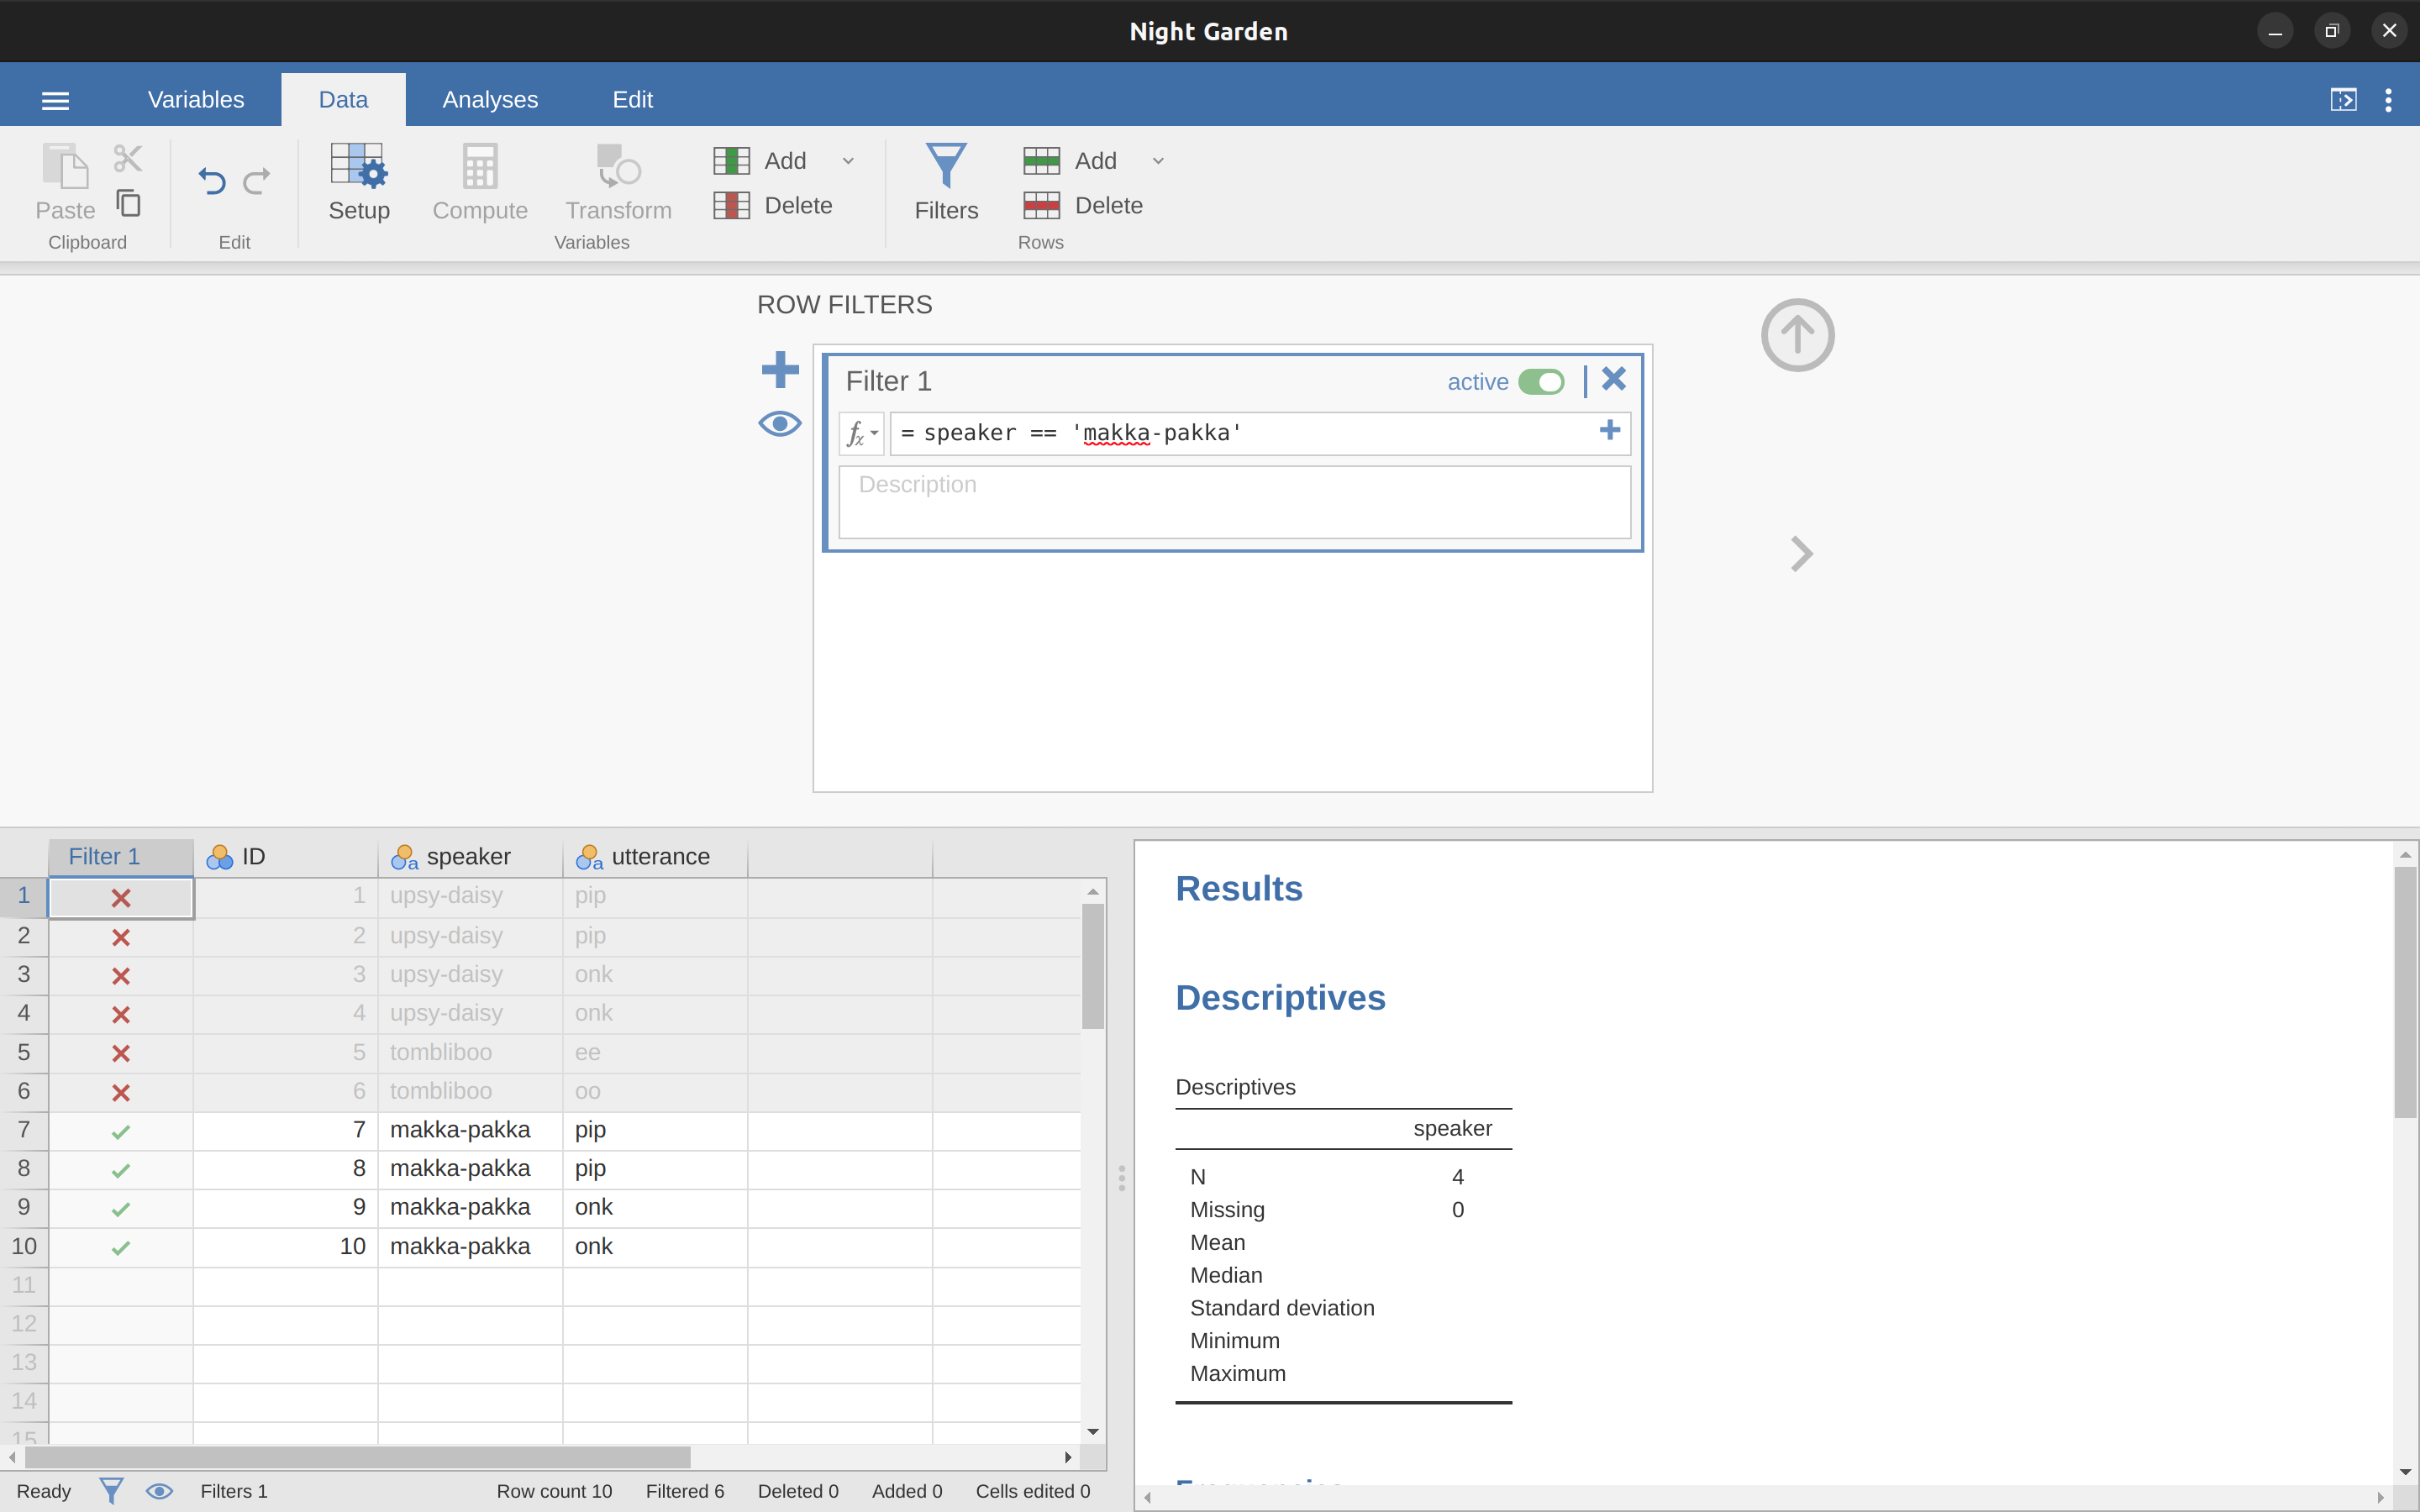
\includegraphics{./images/fig6-10.png} \hfill{}

\caption{\label{fig-fig6-10}Creating a subset of the nightgarden data
using the jamovi `Filters' option}

\end{figure}

When you have done this, you will see that a new column has been added
to the spreadsheet window (see Figure~\ref{fig-fig6-10}), labelled
`Filter 1', with the cases where speaker is not `makka-pakka' greyed-out
(i.e., filtered out) and, conversely, the cases where speaker is
`makka-pakka' have a green check mark indicating they are filtered in.
You can test this by running `Exploration' - `Descriptives' - `Frequency
tables' for the speaker variable and seeing what that shows. Go on, try
it!

Following on from this simple example, you can also build up more
complex filters using logical expressions in jamovi. For instance,
suppose I wanted to keep only those cases when the utterance is either
``pip'' or ``oo''. In this case in the `Filter 1' text box, next to the
`=' sign, you would type the following:

utterance == `pip' or utterance == `oo'

\hypertarget{summary-4}{%
\section{Summary}\label{summary-4}}

Obviously, there's no real coherence to this chapter. It's just a grab
bag of topics and tricks that can be handy to know about, so the best
wrap up I can give here is just to repeat this list:

\begin{itemize}
\tightlist
\item
  \protect\hyperlink{sec-Tabulating-and-cross-tabulating-data}{Tabulating
  and cross-tabulating data}
\item
  \protect\hyperlink{logical-expressions-in-jamovi}{Logical expressions
  in jamovi}
\item
  \protect\hyperlink{sec-Transforming-and-recoding-a-variable}{Transforming
  and recoding a variable}
\item
  \protect\hyperlink{a-few-more-mathematical-functions-and-operations}{A
  few more mathematical functions and operations}
\item
  \protect\hyperlink{extracting-a-subset-of-the-data}{Extracting a
  subset of the data}
\end{itemize}

\part{Statistical theory}

\hypertarget{prelude}{%
\chapter*{Prelude}\label{prelude}}
\addcontentsline{toc}{chapter}{Prelude}

Part IV of the book is by far the most theoretical, focusing as it does
on the theory of statistical inference. Over the next three chapters my
goal is to give you an introduction to probability theory, sampling and
estimation in
Chapter~\ref{sec-Estimating-unknown-quantities-from-a-sample} and
statistical hypothesis testing in Chapter~\ref{sec-Hypothesis-testing}.
Before we get started though, I want to say something about the big
picture. Statistical inference is primarily about learning from data.
The goal is no longer merely to describe our data but to use the data to
draw conclusions about the world. To motivate the discussion I want to
spend a bit of time talking about a philosophical puzzle known as the
riddle of induction, because it speaks to an issue that will pop up over
and over again throughout the book: statistical inference relies on
assumptions. This sounds like a bad thing. In everyday life people say
things like ``you should never make assumptions'', and psychology
classes often talk about assumptions and biases as bad things that we
should try to avoid. From bitter personal experience I have learned
never to say such things around philosophers!

\hypertarget{on-the-limits-of-logical-reasoning}{%
\section*{On the limits of logical
reasoning}\label{on-the-limits-of-logical-reasoning}}
\addcontentsline{toc}{section}{On the limits of logical reasoning}

\begin{quote}
\emph{The whole art of war consists in getting at what is on the other
side of the hill, or, in other words, in learning what we do not know
from what we do.}\\
- Arthur Wellesley, 1st Duke of Wellington
\end{quote}

I am told that quote above came about as a consequence of a carriage
ride across the countryside.\footnote{\href{\%0A\%20http://www.bartleby.com/344/400.html}{http://www.bartleby.com/344/400.html}}
He and his companion, J. W. Croker, were playing a guessing game, each
trying to predict what would be on the other side of each hill. In every
case it turned out that Wellesley was right and Croker was wrong. Many
years later when Wellesley was asked about the game he explained that
``the whole art of war consists in getting at what is on the other side
of the hill''. Indeed, war is not special in this respect. All of life
is a guessing game of one form or another, and getting by on a day to
day basis requires us to make good guesses. So let's play a guessing
game of our own.

Suppose you and I are observing the Wellesley-Croker competition and
after every three hills you and I have to predict who will win the next
one, Wellesley or Croker. Let's say that W refers to a Wellesley victory
and C refers to a Croker victory. After three hills, our data set looks
like this:

\(WWW\)

Our conversation goes like this:

\begin{quote}
you: Three in a row doesn't mean much. I suppose Wellesley might be
better at this than Croker, but it might just be luck. Still, I'm a bit
of a gambler. I'll bet on Wellesley.
\end{quote}

\begin{quote}
me: I agree that three in a row isn't informative and I see no reason to
prefer Wellesley's guesses over Croker's. I can't justify betting at
this stage. Sorry. No bet for me.
\end{quote}

Your gamble paid off: three more hills go by and Wellesley wins all
three. Going into the next round of our game the score is 1-0 in favour
of you and our data set looks like this: \(WWW\) \(WWW\) I've organised
the data into blocks of three so that you can see which batch
corresponds to the observations that we had available at each step in
our little side game. After seeing this new batch, our conversation
continues:

\begin{quote}
you: Six wins in a row for Duke Wellesley. This is starting to feel a
bit suspicious. I'm still not certain, but I reckon that he's going to
win the next one too.
\end{quote}

\begin{quote}
me: I guess I don't see that. Sure, I agree that Wellesley has won six
in a row, but I don't see any logical reason why that means he'll win
the seventh one. No bet. you: Do you really think so? Fair enough, but
my bet worked out last time and I'm okay with my choice.
\end{quote}

For a second time you were right, and for a second time I was wrong.
Wellesley wins the next three hills, extending his winning record
against Croker to 9-0. The data set available to us is now this: \(WWW\)
\(WWW\) \(WWW\) And our conversation goes like this:

\begin{quote}
you: Okay, this is pretty obvious. Wellesley is way better at this game.
We both agree he's going to win the next hill, right?
\end{quote}

\begin{quote}
me: Is there really any logical evidence for that? Before we started
this game, there were lots of possibilities for the first 10 outcomes,
and I had no idea which one to expect. \(WWW\) \(WWW\) \(WWW\) \(W\) was
one possibility, but so was \(WCC\) \(CWC\) \(WWC\) \(C\) and \(WWW\)
\(WWW\) \(WWW\) \(C\) or even \(CCC\) \(CCC\) \(CCC\) \(C\). Because I
had no idea what would happen so I'd have said they were all equally
likely. I assume you would have too, right? I mean, that's what it means
to say you have ``no idea'', isn't it?
\end{quote}

\begin{quote}
you: I suppose so.
\end{quote}

\begin{quote}
me: Well then, the observations we've made logically rule out all
possibilities except two: \(WWW\) \(WWW\) \(WWW\) \(C\) or \(WWW\)
\(WWW\) \(WWW\) \(W\). Both of these are perfectly consistent with the
evidence we've encountered so far, aren't they?
\end{quote}

\begin{quote}
you: Yes, of course they are. Where are you going with this? me: So
what's changed then? At the start of our game, you'd have agreed with me
that these are equally plausible and none of the evidence that we've
encountered has discriminated between these two possibilities.
Therefore, both of these possibilities remain equally plausible and I
see no logical reason to prefer one over the other. So yes, while I
agree with you that Wellesley's run of 9 wins in a row is remarkable, I
can't think of a good reason to think he'll win the 10th hill. No bet.
\end{quote}

\begin{quote}
you: I see your point, but I'm still willing to chance it. I'm betting
on Wellesley.
\end{quote}

Wellesley's winning streak continues for the next three hills. The score
in the Wellesley-Croker game is now 12-0, and the score in our game is
now 3-0. As we approach the fourth round of our game, our data set is
this: \(WWW\) \(WWW\) \(WWW\) \(WWW\) and the conversation continues:

\begin{quote}
you: Oh yeah! Three more wins for Wellesley and another victory for me.
Admit it, I was right about him! I guess we're both betting on Wellesley
this time around, right?
\end{quote}

\begin{quote}
me: I don't know what to think. I feel like we're in the same situation
we were in last round, and nothing much has changed. There are only two
legitimate possibilities for a sequence of 13 hills that haven't already
been ruled out, \(WWW\) \(WWW\) \(WWW\) \(WWW\) \(C\) and \(WWW\)
\(WWW\) \(WWW\) \(WWW\) \(W\). It's just like I said last time. If all
possible outcomes were equally sensible before the game started,
shouldn't these two be equally sensible now given that our observations
don't rule out either one? I agree that it feels like Wellesley is on an
amazing winning streak, but where's the logical evidence that the streak
will continue?
\end{quote}

\begin{quote}
you: I think you're being unreasonable. Why not take a look at our
scorecard, if you need evidence? You're the expert on statistics and
you've been using this fancy logical analysis, but the fact is you're
losing. I'm just relying on common sense and I'm winning. Maybe you
should switch strategies.
\end{quote}

\begin{quote}
me: Hmm, that is a good point and I don't want to lose the game, but I'm
afraid I don't see any logical evidence that your strategy is better
than mine. It seems to me that if there were someone else watching our
game, what they'd have observed is a run of three wins to you. Their
data would look like this: \(YYY\). Logically, I don't see that this is
any different to our first round of watching Wellesley and Croker. Three
wins to you doesn't seem like a lot of evidence, and I see no reason to
think that your strategy is working out any better than mine. If I
didn't think that \(WWW\) was good evidence then for Wellesley being
better than Croker at their game, surely I have no reason now to think
that YYY is good evidence that you're better at ours?
\end{quote}

\begin{quote}
you: Okay, now I think you're being a jerk.
\end{quote}

\begin{quote}
me: I don't see the logical evidence for that.
\end{quote}

\hypertarget{learning-without-making-assumptions-is-a-myth}{%
\section*{Learning without making assumptions is a
myth}\label{learning-without-making-assumptions-is-a-myth}}
\addcontentsline{toc}{section}{Learning without making assumptions is a
myth}

There are lots of different ways in which we could dissect this
dialogue, but since this is a statistics book pitched at psychologists
and not an introduction to the philosophy and psychology of reasoning,
I'll keep it brief. What I've described above is sometimes referred to
as the riddle of induction. It seems entirely reasonable to think that a
12-0 winning record by Wellesley is pretty strong evidence that he will
win the 13th game, but it is not easy to provide a proper logical
justification for this belief. On the contrary, despite the obviousness
of the answer, it's not actually possible to justify betting on
Wellesley without relying on some assumption that you don't have any
logical justification for.

The riddle of induction is most associated with the philosophical work
of David Hume and more recently Nelson Goodman, but you can find
examples of the problem popping up in fields as diverse as literature
(Lewis Carroll) and machine learning (the ``no free lunch'' theorem).
There really is something weird about trying to ``learn what we do not
know from what we do know''. The critical point is that assumptions and
biases are unavoidable if you want to learn anything about the world.
There is no escape from this, and it is just as true for statistical
inference as it is for human reasoning. In the dialogue I was taking aim
at your perfectly sensible inferences as a human being, but the common
sense reasoning that you relied on is no different to what a
statistician would have done. Your ``common sense'' half of the dialog
relied on an implicit assumption that there exists some difference in
skill between Wellesley and Croker, and what you were doing was trying
to work out what that difference in skill level would be. My ``logical
analysis'' rejects that assumption entirely. All I was willing to accept
is that there are sequences of wins and losses and that I did not know
which sequences would be observed. Throughout the dialogue I kept
insisting that all logically possible data sets were equally plausible
at the start of the Wellesely-Croker game, and the only way in which I
ever revised my beliefs was to eliminate those possibilities that were
factually inconsistent with the observations.

That sounds perfectly sensible on its own terms. In fact, it even sounds
like the hallmark of good deductive reasoning. Like Sherlock Holmes, my
approach was to rule out that which is impossible in the hope that what
would be left is the truth. Yet as we saw, ruling out the impossible
never led me to make a prediction. On its own terms everything I said in
my half of the dialogue was entirely correct. An inability to make any
predictions is the logical consequence of making ``no assumptions''. In
the end I lost our game because you did make some assumptions and those
assumptions turned out to be right. Skill is a real thing, and because
you believed in the existence of skill you were able to learn that
Wellesley had more of it than Croker. Had you relied on a less sensible
assumption to drive your learning you might not have won the game.

Ultimately there are two things you should take away from this. First,
as I've said, you cannot avoid making assumptions if you want to learn
anything from your data. But second, once you realise that assumptions
are necessary it becomes important to make sure you make the right ones!
A data analysis that relies on few assumptions is not necessarily better
than one that makes many assumptions, it all depends on whether those
assumptions are good ones for your data. As we go through the rest of
this book I'll often point out the assumptions that underpin a
particular statistical technique, and how you can check whether those
assumptions are sensible.

\begin{center}\rule{0.5\linewidth}{0.5pt}\end{center}

\hypertarget{sec-Introduction-to-probability}{%
\chapter{Introduction to
probability}\label{sec-Introduction-to-probability}}

\begin{quote}
\emph{{[}God{]} has afforded us only the twilight \ldots{} of
Probability.}\\
-- John Locke
\end{quote}

Up to this point in the book we've discussed some of the key ideas in
experimental design, and we've talked a little about how you can
summarise a data set. To a lot of people this is all there is to
statistics: collecting all the numbers, calculating averages, drawing
pictures, and putting them all in a report somewhere. Kind of like stamp
collecting but with numbers. However, statistics covers much more than
that. In fact, descriptive statistics is one of the smallest parts of
statistics and one of the least powerful. The bigger and more useful
part of statistics is that it provides information that lets you make
inferences about data.

Once you start thinking about statistics in these terms, that statistics
is there to help us draw inferences from data, you start seeing examples
of it everywhere. For instance, here's a tiny extract from a newspaper
article in the Sydney Morning Herald (30 Oct 2010):

\begin{quote}
``I have a tough job,'' the Premier said in response to a poll which
found her government is now the most unpopular Labor administration in
polling history, with a primary vote of just 23 per cent.
\end{quote}

This kind of remark is entirely unremarkable in the papers or in
everyday life, but let's have a think about what it entails. A polling
company has conducted a survey, usually a pretty big one because they
can afford it. I'm too lazy to track down the original survey so let's
just imagine that they called 1000 New South Wales (NSW) voters at
random, and 230 (23\%) of those claimed that they intended to vote for
the Australian Labor Party (ALP). For the 2010 Federal election the
Australian Electoral Commission reported 4,610,795 enrolled voters in
NSW, so the opinions of the remaining 4,609,795 voters (about 99.98\% of
voters) remain unknown to us. Even assuming that no-one lied to the
polling company the only thing we can say with 100\% confidence is that
the true ALP primary vote is somewhere between 230/4610795 (about
0.005\%) and 4610025/4610795 (about 99.83\%). So, on what basis is it
legitimate for the polling company, the newspaper, and the readership to
conclude that the ALP primary vote is only about 23\%?

The answer to the question is pretty obvious. If I call 1000 people at
random, and 230 of them say they intend to vote for the ALP, then it
seems very unlikely that these are the only 230 people out of the entire
voting public who actually intend to vote ALP. In other words, we assume
that the data collected by the polling company is pretty representative
of the population at large. But how representative? Would we be
surprised to discover that the true ALP primary vote is actually 24\%?
29\%? 37\%? At this point everyday intuition starts to break down a bit.
No-one would be surprised by 24\%, and everybody would be surprised by
37\%, but it's a bit hard to say whether 29\% is plausible. We need some
more powerful tools than just looking at the numbers and guessing.

\textbf{Inferential statistics} provides the tools that we need to
answer these sorts of questions, and since these kinds of questions lie
at the heart of the scientific enterprise, they take up the lions share
of every introductory course on statistics and research methods.
However, the theory of statistical inference is built on top of
\textbf{probability theory}. And it is to probability theory that we
must now turn. This discussion of probability theory is basically
background detail. There's not a lot of statistics per se in this
chapter, and you don't need to understand this material in as much depth
as the other chapters in this part of the book. Nevertheless, because
probability theory does underpin so much of statistics, it's worth
covering some of the basics.

\hypertarget{how-are-probability-and-statistics-different}{%
\section{How are probability and statistics
different?}\label{how-are-probability-and-statistics-different}}

Before we start talking about probability theory, it's helpful to spend
a moment thinking about the relationship between probability and
statistics. The two disciplines are closely related but they're not
identical. Probability theory is ``the doctrine of chances''. It's a
branch of mathematics that tells you how often different kinds of events
will happen. For example, all of these questions are things you can
answer using probability theory:

\begin{itemize}
\tightlist
\item
  What are the chances of a fair coin coming up heads 10 times in a row?
\item
  If I roll a six sided dice twice, how likely is it that I'll roll two
  sixes?
\item
  How likely is it that five cards drawn from a perfectly shuffled deck
  will all be hearts?
\item
  What are the chances that I'll win the lottery?
\end{itemize}

Notice that all of these questions have something in common. In each
case the ``truth of the world'' is known and my question relates to the
``what kind of events'' will happen. In the first question I know that
the coin is fair so there's a 50\% chance that any individual coin flip
will come up heads. In the second question I know that the chance of
rolling a 6 on a single die is 1 in 6. In the third question I know that
the deck is shuffled properly. And in the fourth question I know that
the lottery follows specific rules. You get the idea. The critical point
is that probabilistic questions start with a known \textbf{model} of the
world, and we use that model to do some calculations. The underlying
model can be quite simple. For instance, in the coin flipping example we
can write down the model like this:

\[P(head)=0.5\]

which you can read as ``the probability of heads is 0.5''. As we'll see
later, in the same way that percentages are numbers that range from 0\%
to 100\%, probabilities are just numbers that range from 0 to 1. When
using this probability model to answer the first question I don't
actually know exactly what's going to happen. Maybe I'll get 10 heads,
like the question says. But maybe I'll get three heads. That's the key
thing. In probability theory the model is known but the data are not.

So that's probability. What about statistics? Statistical questions work
the other way around. In statistics we do not know the truth about the
world. All we have is the data and it is from the data that we want to
learn the truth about the world. Statistical questions tend to look more
like these:

\begin{itemize}
\tightlist
\item
  If my friend flips a coin 10 times and gets 10 heads are they playing
  a trick on me?
\item
  If five cards off the top of the deck are all hearts how likely is it
  that the deck was shuffled?
\item
  If the lottery commissioner's spouse wins the lottery how likely is it
  that the lottery was rigged?
\end{itemize}

This time around the only thing we have are data. What I know is that I
saw my friend flip the coin 10 times and it came up heads every time.
And what I want to infer is whether or not I should conclude that what I
just saw was actually a fair coin being flipped 10 times in a row, or
whether I should suspect that my friend is playing a trick on me. The
data I have look like this:

H H H H H H H H H H H

and what I'm trying to do is work out which ``model of the world'' I
should put my trust in. If the coin is fair then the model I should
adopt is one that says that the probability of heads is 0.5, that is
P(heads) = 0.5. If the coin is not fair then I should conclude that the
probability of heads is not 0.5, which we would write as
\(P(heads)\ne{0.5}\). In other words, the statistical inference problem
is to figure out which of these probability models is right. Clearly,
the statistical question isn't the same as the probability question, but
they're deeply connected to one another. Because of this, a good
introduction to statistical theory will start with a discussion of what
probability is and how it works.

\hypertarget{what-does-probability-mean}{%
\section{What does probability mean?}\label{what-does-probability-mean}}

Let's start with the first of these questions. What is ``probability''?
It might seem surprising to you but while statisticians and
mathematicians (mostly) agree on what the rules of probability are,
there's much less of a consensus on what the word really means. It seems
weird because we're all very comfortable using words like ``chance'',
``likely'', ``possible'' and ``probable'', and it doesn't seem like it
should be a very difficult question to answer. But if you've ever had
that experience in real life you might walk away from the conversation
feeling like you didn't quite get it right, and that (like many everyday
concepts) it turns out that you don't really know what it's all about.

So I'll have a go at it. Let's suppose I want to bet on a soccer game
between two teams of robots, Arduino Arsenal and C Milan. After thinking
about it, I decide that there is an 80\% probability of Arduino Arsenal
winning. What do I mean by that? Here are three possibilities:

\begin{itemize}
\tightlist
\item
  They're robot teams so I can make them play over and over again, and
  if I did that Arduino Arsenal would win 8 out of every 10 games on
  average.
\item
  For any given game, I would agree that betting on this game is only
  ``fair'' if a \$1 bet on C Milan gives a \$5 payoff (i.e.~I get my \$1
  back plus a \$4 reward for being correct), as would a \$4 bet on
  Arduino Arsenal (i.e., my \$4 bet plus a \$1 reward).
\item
  My subjective ``belief'' or ``confidence'' in an Arduino Arsenal
  victory is four times as strong as my belief in a C Milan victory.
\end{itemize}

Each of these seems sensible. However, they're not identical and not
every statistician would endorse all of them. The reason is that there
are different statistical ideologies (yes, really!) and depending on
which one you subscribe to, you might say that some of those statements
are meaningless or irrelevant. In this section I give a brief
introduction the two main approaches that exist in the literature. These
are by no means the only approaches, but they're the two big ones.

\hypertarget{the-frequentist-view}{%
\subsection{The frequentist view}\label{the-frequentist-view}}

The first of the two major approaches to probability, and the more
dominant one in statistics, is referred to as the \textbf{frequentist
view} and it defines probability as a \textbf{long-run frequency}.
Suppose we were to try flipping a fair coin over and over again. By
definition this is a coin that has \(P(H) = 0.5\). What might we
observe? One possibility is that the first 20 flips might look like
this:

T,H,H,H,H,T,T,H,H,H,H,T,H,H,T,T,T,T,T,H

In this case 11 of these 20 coin flips (55\%) came up heads. Now suppose
that I'd been keeping a running tally of the number of heads (which I'll
call \(N_H\)) that I've seen, across the first N flips, and calculate
the proportion of heads \(\frac{N_H}{N}\) every time.
Table~\ref{tbl-tab7-1} shows what I'd get (I did literally flip coins to
produce this!):

\hypertarget{tbl-tab7-1}{}
 
  \providecommand{\huxb}[2]{\arrayrulecolor[RGB]{#1}\global\arrayrulewidth=#2pt}
  \providecommand{\huxvb}[2]{\color[RGB]{#1}\vrule width #2pt}
  \providecommand{\huxtpad}[1]{\rule{0pt}{#1}}
  \providecommand{\huxbpad}[1]{\rule[-#1]{0pt}{#1}}

\begin{table}[ht]
\caption{\label{tbl-tab7-1}Coin flips and proportion of heads }\tabularnewline

\begin{centerbox}
\begin{threeparttable}
\setlength{\tabcolsep}{0pt}
\begin{tabularx}{0.9\textwidth}{p{0.075\textwidth} p{0.075\textwidth} p{0.075\textwidth} p{0.075\textwidth} p{0.075\textwidth} p{0.075\textwidth} p{0.075\textwidth} p{0.075\textwidth} p{0.075\textwidth} p{0.075\textwidth} p{0.075\textwidth} p{0.075\textwidth}}


\hhline{>{\huxb{0, 0, 0}{0.4}}->{\huxb{0, 0, 0}{0.4}}->{\huxb{0, 0, 0}{0.4}}->{\huxb{0, 0, 0}{0.4}}->{\huxb{0, 0, 0}{0.4}}->{\huxb{0, 0, 0}{0.4}}->{\huxb{0, 0, 0}{0.4}}->{\huxb{0, 0, 0}{0.4}}->{\huxb{0, 0, 0}{0.4}}->{\huxb{0, 0, 0}{0.4}}->{\huxb{0, 0, 0}{0.4}}->{\huxb{0, 0, 0}{0.4}}-}
\arrayrulecolor{black}

\multicolumn{2}{!{\huxvb{0, 0, 0}{0}}p{0.15\textwidth+2\tabcolsep}!{\huxvb{0, 0, 0}{0}}}{\cellcolor[RGB]{242, 242, 242}\hspace{0pt}\parbox[b]{0.15\textwidth+2\tabcolsep-0pt-6pt}{\huxtpad{6pt + 1em}\centering \textbf{number of flips}\huxbpad{6pt}}} &
\multicolumn{1}{p{0.075\textwidth}!{\huxvb{0, 0, 0}{0}}}{\cellcolor[RGB]{242, 242, 242}\hspace{6pt}\parbox[b]{0.075\textwidth-6pt-6pt}{\huxtpad{6pt + 1em}\centering \textbf{1}\huxbpad{6pt}}} &
\multicolumn{1}{p{0.075\textwidth}!{\huxvb{0, 0, 0}{0}}}{\cellcolor[RGB]{242, 242, 242}\hspace{6pt}\parbox[b]{0.075\textwidth-6pt-6pt}{\huxtpad{6pt + 1em}\centering \textbf{2}\huxbpad{6pt}}} &
\multicolumn{1}{p{0.075\textwidth}!{\huxvb{0, 0, 0}{0}}}{\cellcolor[RGB]{242, 242, 242}\hspace{6pt}\parbox[b]{0.075\textwidth-6pt-6pt}{\huxtpad{6pt + 1em}\centering \textbf{3}\huxbpad{6pt}}} &
\multicolumn{1}{p{0.075\textwidth}!{\huxvb{0, 0, 0}{0}}}{\cellcolor[RGB]{242, 242, 242}\hspace{6pt}\parbox[b]{0.075\textwidth-6pt-6pt}{\huxtpad{6pt + 1em}\centering \textbf{4}\huxbpad{6pt}}} &
\multicolumn{1}{p{0.075\textwidth}!{\huxvb{0, 0, 0}{0}}}{\cellcolor[RGB]{242, 242, 242}\hspace{6pt}\parbox[b]{0.075\textwidth-6pt-6pt}{\huxtpad{6pt + 1em}\centering \textbf{5}\huxbpad{6pt}}} &
\multicolumn{1}{p{0.075\textwidth}!{\huxvb{0, 0, 0}{0}}}{\cellcolor[RGB]{242, 242, 242}\hspace{6pt}\parbox[b]{0.075\textwidth-6pt-6pt}{\huxtpad{6pt + 1em}\centering \textbf{6}\huxbpad{6pt}}} &
\multicolumn{1}{p{0.075\textwidth}!{\huxvb{0, 0, 0}{0}}}{\cellcolor[RGB]{242, 242, 242}\hspace{6pt}\parbox[b]{0.075\textwidth-6pt-6pt}{\huxtpad{6pt + 1em}\centering \textbf{7}\huxbpad{6pt}}} &
\multicolumn{1}{p{0.075\textwidth}!{\huxvb{0, 0, 0}{0}}}{\cellcolor[RGB]{242, 242, 242}\hspace{6pt}\parbox[b]{0.075\textwidth-6pt-6pt}{\huxtpad{6pt + 1em}\centering \textbf{8}\huxbpad{6pt}}} &
\multicolumn{1}{p{0.075\textwidth}!{\huxvb{0, 0, 0}{0}}}{\cellcolor[RGB]{242, 242, 242}\hspace{6pt}\parbox[b]{0.075\textwidth-6pt-6pt}{\huxtpad{6pt + 1em}\centering \textbf{9}\huxbpad{6pt}}} &
\multicolumn{1}{p{0.075\textwidth}!{\huxvb{0, 0, 0}{0}}}{\cellcolor[RGB]{242, 242, 242}\hspace{6pt}\parbox[b]{0.075\textwidth-6pt-0pt}{\huxtpad{6pt + 1em}\centering \textbf{10}\huxbpad{6pt}}} \tabularnewline[-0.5pt]


\hhline{>{\huxb{0, 0, 0}{0.4}}->{\huxb{0, 0, 0}{0.4}}->{\huxb{0, 0, 0}{0.4}}->{\huxb{0, 0, 0}{0.4}}->{\huxb{0, 0, 0}{0.4}}->{\huxb{0, 0, 0}{0.4}}->{\huxb{0, 0, 0}{0.4}}->{\huxb{0, 0, 0}{0.4}}->{\huxb{0, 0, 0}{0.4}}->{\huxb{0, 0, 0}{0.4}}->{\huxb{0, 0, 0}{0.4}}->{\huxb{0, 0, 0}{0.4}}-}
\arrayrulecolor{black}

\multicolumn{2}{!{\huxvb{0, 0, 0}{0}}p{0.15\textwidth+2\tabcolsep}!{\huxvb{0, 0, 0}{0}}}{\hspace{0pt}\parbox[b]{0.15\textwidth+2\tabcolsep-0pt-6pt}{\huxtpad{6pt + 1em}\centering number of heads\huxbpad{6pt}}} &
\multicolumn{1}{p{0.075\textwidth}!{\huxvb{0, 0, 0}{0}}}{\hspace{6pt}\parbox[b]{0.075\textwidth-6pt-6pt}{\huxtpad{6pt + 1em}\centering 0\huxbpad{6pt}}} &
\multicolumn{1}{p{0.075\textwidth}!{\huxvb{0, 0, 0}{0}}}{\hspace{6pt}\parbox[b]{0.075\textwidth-6pt-6pt}{\huxtpad{6pt + 1em}\centering 1\huxbpad{6pt}}} &
\multicolumn{1}{p{0.075\textwidth}!{\huxvb{0, 0, 0}{0}}}{\hspace{6pt}\parbox[b]{0.075\textwidth-6pt-6pt}{\huxtpad{6pt + 1em}\centering 2\huxbpad{6pt}}} &
\multicolumn{1}{p{0.075\textwidth}!{\huxvb{0, 0, 0}{0}}}{\hspace{6pt}\parbox[b]{0.075\textwidth-6pt-6pt}{\huxtpad{6pt + 1em}\centering 3\huxbpad{6pt}}} &
\multicolumn{1}{p{0.075\textwidth}!{\huxvb{0, 0, 0}{0}}}{\hspace{6pt}\parbox[b]{0.075\textwidth-6pt-6pt}{\huxtpad{6pt + 1em}\centering 4\huxbpad{6pt}}} &
\multicolumn{1}{p{0.075\textwidth}!{\huxvb{0, 0, 0}{0}}}{\hspace{6pt}\parbox[b]{0.075\textwidth-6pt-6pt}{\huxtpad{6pt + 1em}\centering 4\huxbpad{6pt}}} &
\multicolumn{1}{p{0.075\textwidth}!{\huxvb{0, 0, 0}{0}}}{\hspace{6pt}\parbox[b]{0.075\textwidth-6pt-6pt}{\huxtpad{6pt + 1em}\centering 4\huxbpad{6pt}}} &
\multicolumn{1}{p{0.075\textwidth}!{\huxvb{0, 0, 0}{0}}}{\hspace{6pt}\parbox[b]{0.075\textwidth-6pt-6pt}{\huxtpad{6pt + 1em}\centering 5\huxbpad{6pt}}} &
\multicolumn{1}{p{0.075\textwidth}!{\huxvb{0, 0, 0}{0}}}{\hspace{6pt}\parbox[b]{0.075\textwidth-6pt-6pt}{\huxtpad{6pt + 1em}\centering 6\huxbpad{6pt}}} &
\multicolumn{1}{p{0.075\textwidth}!{\huxvb{0, 0, 0}{0}}}{\hspace{6pt}\parbox[b]{0.075\textwidth-6pt-0pt}{\huxtpad{6pt + 1em}\centering 7\huxbpad{6pt}}} \tabularnewline[-0.5pt]


\hhline{}
\arrayrulecolor{black}

\multicolumn{2}{!{\huxvb{0, 0, 0}{0}}p{0.15\textwidth+2\tabcolsep}!{\huxvb{0, 0, 0}{0}}}{\cellcolor[RGB]{242, 242, 242}\hspace{0pt}\parbox[b]{0.15\textwidth+2\tabcolsep-0pt-6pt}{\huxtpad{6pt + 1em}\centering proportion\huxbpad{6pt}}} &
\multicolumn{1}{p{0.075\textwidth}!{\huxvb{0, 0, 0}{0}}}{\cellcolor[RGB]{242, 242, 242}\hspace{6pt}\parbox[b]{0.075\textwidth-6pt-6pt}{\huxtpad{6pt + 1em}\centering 0\huxbpad{6pt}}} &
\multicolumn{1}{p{0.075\textwidth}!{\huxvb{0, 0, 0}{0}}}{\cellcolor[RGB]{242, 242, 242}\hspace{6pt}\parbox[b]{0.075\textwidth-6pt-6pt}{\huxtpad{6pt + 1em}\centering 0.5\huxbpad{6pt}}} &
\multicolumn{1}{p{0.075\textwidth}!{\huxvb{0, 0, 0}{0}}}{\cellcolor[RGB]{242, 242, 242}\hspace{6pt}\parbox[b]{0.075\textwidth-6pt-6pt}{\huxtpad{6pt + 1em}\centering 0.67\huxbpad{6pt}}} &
\multicolumn{1}{p{0.075\textwidth}!{\huxvb{0, 0, 0}{0}}}{\cellcolor[RGB]{242, 242, 242}\hspace{6pt}\parbox[b]{0.075\textwidth-6pt-6pt}{\huxtpad{6pt + 1em}\centering 0.75\huxbpad{6pt}}} &
\multicolumn{1}{p{0.075\textwidth}!{\huxvb{0, 0, 0}{0}}}{\cellcolor[RGB]{242, 242, 242}\hspace{6pt}\parbox[b]{0.075\textwidth-6pt-6pt}{\huxtpad{6pt + 1em}\centering 0.8\huxbpad{6pt}}} &
\multicolumn{1}{p{0.075\textwidth}!{\huxvb{0, 0, 0}{0}}}{\cellcolor[RGB]{242, 242, 242}\hspace{6pt}\parbox[b]{0.075\textwidth-6pt-6pt}{\huxtpad{6pt + 1em}\centering 0.67\huxbpad{6pt}}} &
\multicolumn{1}{p{0.075\textwidth}!{\huxvb{0, 0, 0}{0}}}{\cellcolor[RGB]{242, 242, 242}\hspace{6pt}\parbox[b]{0.075\textwidth-6pt-6pt}{\huxtpad{6pt + 1em}\centering 0.57\huxbpad{6pt}}} &
\multicolumn{1}{p{0.075\textwidth}!{\huxvb{0, 0, 0}{0}}}{\cellcolor[RGB]{242, 242, 242}\hspace{6pt}\parbox[b]{0.075\textwidth-6pt-6pt}{\huxtpad{6pt + 1em}\centering 0.63\huxbpad{6pt}}} &
\multicolumn{1}{p{0.075\textwidth}!{\huxvb{0, 0, 0}{0}}}{\cellcolor[RGB]{242, 242, 242}\hspace{6pt}\parbox[b]{0.075\textwidth-6pt-6pt}{\huxtpad{6pt + 1em}\centering 0.67\huxbpad{6pt}}} &
\multicolumn{1}{p{0.075\textwidth}!{\huxvb{0, 0, 0}{0}}}{\cellcolor[RGB]{242, 242, 242}\hspace{6pt}\parbox[b]{0.075\textwidth-6pt-0pt}{\huxtpad{6pt + 1em}\centering 0.7\huxbpad{6pt}}} \tabularnewline[-0.5pt]


\hhline{>{\huxb{0, 0, 0}{0.4}}->{\huxb{0, 0, 0}{0.4}}->{\huxb{0, 0, 0}{0.4}}->{\huxb{0, 0, 0}{0.4}}->{\huxb{0, 0, 0}{0.4}}->{\huxb{0, 0, 0}{0.4}}->{\huxb{0, 0, 0}{0.4}}->{\huxb{0, 0, 0}{0.4}}->{\huxb{0, 0, 0}{0.4}}->{\huxb{0, 0, 0}{0.4}}->{\huxb{0, 0, 0}{0.4}}->{\huxb{0, 0, 0}{0.4}}-}
\arrayrulecolor{black}

\multicolumn{2}{!{\huxvb{0, 0, 0}{0}}p{0.15\textwidth+2\tabcolsep}!{\huxvb{0, 0, 0}{0}}}{\hspace{0pt}\parbox[b]{0.15\textwidth+2\tabcolsep-0pt-6pt}{\huxtpad{6pt + 1em}\centering \textbf{number of flips}\huxbpad{6pt}}} &
\multicolumn{1}{p{0.075\textwidth}!{\huxvb{0, 0, 0}{0}}}{\hspace{6pt}\parbox[b]{0.075\textwidth-6pt-6pt}{\huxtpad{6pt + 1em}\centering \textbf{11}\huxbpad{6pt}}} &
\multicolumn{1}{p{0.075\textwidth}!{\huxvb{0, 0, 0}{0}}}{\hspace{6pt}\parbox[b]{0.075\textwidth-6pt-6pt}{\huxtpad{6pt + 1em}\centering \textbf{12}\huxbpad{6pt}}} &
\multicolumn{1}{p{0.075\textwidth}!{\huxvb{0, 0, 0}{0}}}{\hspace{6pt}\parbox[b]{0.075\textwidth-6pt-6pt}{\huxtpad{6pt + 1em}\centering \textbf{13}\huxbpad{6pt}}} &
\multicolumn{1}{p{0.075\textwidth}!{\huxvb{0, 0, 0}{0}}}{\hspace{6pt}\parbox[b]{0.075\textwidth-6pt-6pt}{\huxtpad{6pt + 1em}\centering \textbf{14}\huxbpad{6pt}}} &
\multicolumn{1}{p{0.075\textwidth}!{\huxvb{0, 0, 0}{0}}}{\hspace{6pt}\parbox[b]{0.075\textwidth-6pt-6pt}{\huxtpad{6pt + 1em}\centering \textbf{15}\huxbpad{6pt}}} &
\multicolumn{1}{p{0.075\textwidth}!{\huxvb{0, 0, 0}{0}}}{\hspace{6pt}\parbox[b]{0.075\textwidth-6pt-6pt}{\huxtpad{6pt + 1em}\centering \textbf{16}\huxbpad{6pt}}} &
\multicolumn{1}{p{0.075\textwidth}!{\huxvb{0, 0, 0}{0}}}{\hspace{6pt}\parbox[b]{0.075\textwidth-6pt-6pt}{\huxtpad{6pt + 1em}\centering \textbf{17}\huxbpad{6pt}}} &
\multicolumn{1}{p{0.075\textwidth}!{\huxvb{0, 0, 0}{0}}}{\hspace{6pt}\parbox[b]{0.075\textwidth-6pt-6pt}{\huxtpad{6pt + 1em}\centering \textbf{18}\huxbpad{6pt}}} &
\multicolumn{1}{p{0.075\textwidth}!{\huxvb{0, 0, 0}{0}}}{\hspace{6pt}\parbox[b]{0.075\textwidth-6pt-6pt}{\huxtpad{6pt + 1em}\centering \textbf{19}\huxbpad{6pt}}} &
\multicolumn{1}{p{0.075\textwidth}!{\huxvb{0, 0, 0}{0}}}{\hspace{6pt}\parbox[b]{0.075\textwidth-6pt-0pt}{\huxtpad{6pt + 1em}\centering \textbf{20}\huxbpad{6pt}}} \tabularnewline[-0.5pt]


\hhline{>{\huxb{0, 0, 0}{0.4}}->{\huxb{0, 0, 0}{0.4}}->{\huxb{0, 0, 0}{0.4}}->{\huxb{0, 0, 0}{0.4}}->{\huxb{0, 0, 0}{0.4}}->{\huxb{0, 0, 0}{0.4}}->{\huxb{0, 0, 0}{0.4}}->{\huxb{0, 0, 0}{0.4}}->{\huxb{0, 0, 0}{0.4}}->{\huxb{0, 0, 0}{0.4}}->{\huxb{0, 0, 0}{0.4}}->{\huxb{0, 0, 0}{0.4}}-}
\arrayrulecolor{black}

\multicolumn{2}{!{\huxvb{0, 0, 0}{0}}p{0.15\textwidth+2\tabcolsep}!{\huxvb{0, 0, 0}{0}}}{\cellcolor[RGB]{242, 242, 242}\hspace{0pt}\parbox[b]{0.15\textwidth+2\tabcolsep-0pt-6pt}{\huxtpad{6pt + 1em}\centering number of heads\huxbpad{6pt}}} &
\multicolumn{1}{p{0.075\textwidth}!{\huxvb{0, 0, 0}{0}}}{\cellcolor[RGB]{242, 242, 242}\hspace{6pt}\parbox[b]{0.075\textwidth-6pt-6pt}{\huxtpad{6pt + 1em}\centering 8\huxbpad{6pt}}} &
\multicolumn{1}{p{0.075\textwidth}!{\huxvb{0, 0, 0}{0}}}{\cellcolor[RGB]{242, 242, 242}\hspace{6pt}\parbox[b]{0.075\textwidth-6pt-6pt}{\huxtpad{6pt + 1em}\centering 8\huxbpad{6pt}}} &
\multicolumn{1}{p{0.075\textwidth}!{\huxvb{0, 0, 0}{0}}}{\cellcolor[RGB]{242, 242, 242}\hspace{6pt}\parbox[b]{0.075\textwidth-6pt-6pt}{\huxtpad{6pt + 1em}\centering 9\huxbpad{6pt}}} &
\multicolumn{1}{p{0.075\textwidth}!{\huxvb{0, 0, 0}{0}}}{\cellcolor[RGB]{242, 242, 242}\hspace{6pt}\parbox[b]{0.075\textwidth-6pt-6pt}{\huxtpad{6pt + 1em}\centering 10\huxbpad{6pt}}} &
\multicolumn{1}{p{0.075\textwidth}!{\huxvb{0, 0, 0}{0}}}{\cellcolor[RGB]{242, 242, 242}\hspace{6pt}\parbox[b]{0.075\textwidth-6pt-6pt}{\huxtpad{6pt + 1em}\centering 10\huxbpad{6pt}}} &
\multicolumn{1}{p{0.075\textwidth}!{\huxvb{0, 0, 0}{0}}}{\cellcolor[RGB]{242, 242, 242}\hspace{6pt}\parbox[b]{0.075\textwidth-6pt-6pt}{\huxtpad{6pt + 1em}\centering 10\huxbpad{6pt}}} &
\multicolumn{1}{p{0.075\textwidth}!{\huxvb{0, 0, 0}{0}}}{\cellcolor[RGB]{242, 242, 242}\hspace{6pt}\parbox[b]{0.075\textwidth-6pt-6pt}{\huxtpad{6pt + 1em}\centering 10\huxbpad{6pt}}} &
\multicolumn{1}{p{0.075\textwidth}!{\huxvb{0, 0, 0}{0}}}{\cellcolor[RGB]{242, 242, 242}\hspace{6pt}\parbox[b]{0.075\textwidth-6pt-6pt}{\huxtpad{6pt + 1em}\centering 10\huxbpad{6pt}}} &
\multicolumn{1}{p{0.075\textwidth}!{\huxvb{0, 0, 0}{0}}}{\cellcolor[RGB]{242, 242, 242}\hspace{6pt}\parbox[b]{0.075\textwidth-6pt-6pt}{\huxtpad{6pt + 1em}\centering 10\huxbpad{6pt}}} &
\multicolumn{1}{p{0.075\textwidth}!{\huxvb{0, 0, 0}{0}}}{\cellcolor[RGB]{242, 242, 242}\hspace{6pt}\parbox[b]{0.075\textwidth-6pt-0pt}{\huxtpad{6pt + 1em}\centering 11\huxbpad{6pt}}} \tabularnewline[-0.5pt]


\hhline{}
\arrayrulecolor{black}

\multicolumn{2}{!{\huxvb{0, 0, 0}{0}}p{0.15\textwidth+2\tabcolsep}!{\huxvb{0, 0, 0}{0}}}{\hspace{0pt}\parbox[b]{0.15\textwidth+2\tabcolsep-0pt-6pt}{\huxtpad{6pt + 1em}\centering proportion\huxbpad{6pt}}} &
\multicolumn{1}{p{0.075\textwidth}!{\huxvb{0, 0, 0}{0}}}{\hspace{6pt}\parbox[b]{0.075\textwidth-6pt-6pt}{\huxtpad{6pt + 1em}\centering 0.73\huxbpad{6pt}}} &
\multicolumn{1}{p{0.075\textwidth}!{\huxvb{0, 0, 0}{0}}}{\hspace{6pt}\parbox[b]{0.075\textwidth-6pt-6pt}{\huxtpad{6pt + 1em}\centering 0.67\huxbpad{6pt}}} &
\multicolumn{1}{p{0.075\textwidth}!{\huxvb{0, 0, 0}{0}}}{\hspace{6pt}\parbox[b]{0.075\textwidth-6pt-6pt}{\huxtpad{6pt + 1em}\centering 0.69\huxbpad{6pt}}} &
\multicolumn{1}{p{0.075\textwidth}!{\huxvb{0, 0, 0}{0}}}{\hspace{6pt}\parbox[b]{0.075\textwidth-6pt-6pt}{\huxtpad{6pt + 1em}\centering 0.71\huxbpad{6pt}}} &
\multicolumn{1}{p{0.075\textwidth}!{\huxvb{0, 0, 0}{0}}}{\hspace{6pt}\parbox[b]{0.075\textwidth-6pt-6pt}{\huxtpad{6pt + 1em}\centering 0.67\huxbpad{6pt}}} &
\multicolumn{1}{p{0.075\textwidth}!{\huxvb{0, 0, 0}{0}}}{\hspace{6pt}\parbox[b]{0.075\textwidth-6pt-6pt}{\huxtpad{6pt + 1em}\centering 0.63\huxbpad{6pt}}} &
\multicolumn{1}{p{0.075\textwidth}!{\huxvb{0, 0, 0}{0}}}{\hspace{6pt}\parbox[b]{0.075\textwidth-6pt-6pt}{\huxtpad{6pt + 1em}\centering 0.59\huxbpad{6pt}}} &
\multicolumn{1}{p{0.075\textwidth}!{\huxvb{0, 0, 0}{0}}}{\hspace{6pt}\parbox[b]{0.075\textwidth-6pt-6pt}{\huxtpad{6pt + 1em}\centering 0.56\huxbpad{6pt}}} &
\multicolumn{1}{p{0.075\textwidth}!{\huxvb{0, 0, 0}{0}}}{\hspace{6pt}\parbox[b]{0.075\textwidth-6pt-6pt}{\huxtpad{6pt + 1em}\centering 0.53\huxbpad{6pt}}} &
\multicolumn{1}{p{0.075\textwidth}!{\huxvb{0, 0, 0}{0}}}{\hspace{6pt}\parbox[b]{0.075\textwidth-6pt-0pt}{\huxtpad{6pt + 1em}\centering 0.55\huxbpad{6pt}}} \tabularnewline[-0.5pt]


\hhline{>{\huxb{0, 0, 0}{0.4}}->{\huxb{0, 0, 0}{0.4}}->{\huxb{0, 0, 0}{0.4}}->{\huxb{0, 0, 0}{0.4}}->{\huxb{0, 0, 0}{0.4}}->{\huxb{0, 0, 0}{0.4}}->{\huxb{0, 0, 0}{0.4}}->{\huxb{0, 0, 0}{0.4}}->{\huxb{0, 0, 0}{0.4}}->{\huxb{0, 0, 0}{0.4}}->{\huxb{0, 0, 0}{0.4}}->{\huxb{0, 0, 0}{0.4}}-}
\arrayrulecolor{black}
\end{tabularx} 

\end{threeparttable}\par\end{centerbox}

\end{table}
 

Notice that at the start of the sequence the \emph{proportion} of heads
fluctuates wildly, starting at \(.00\) and rising as high as \(.80\).
Later on, one gets the impression that it dampens out a bit, with more
and more of the values actually being pretty close to the ``right''
answer of \(.50\). This is the frequentist definition of probability in
a nutshell. Flip a fair coin over and over again, and as N grows large
(approaches infinity, denoted \(N \rightarrow \infty\) ) the proportion
of heads will converge to 50\%. There are some subtle technicalities
that the mathematicians care about, but qualitatively speaking that's
how the frequentists define probability. Unfortunately, I don't have an
infinite number of coins or the infinite patience required to flip a
coin an infinite number of times. However, I do have a computer and
computers excel at mindless repetitive tasks. So I asked my computer to
simulate flipping a coin 1000 times and then drew a picture of what
happens to the proportion \(\frac{N_H}{N}\) as \(N\) increases.
Actually, I did it four times just to make sure it wasn't a fluke. The
results are shown in Figure~\ref{fig-fig7-1}. As you can see, the
proportion of observed heads eventually stops fluctuating and settles
down. When it does, the number at which it finally settles is the true
probability of heads.

The frequentist definition of probability has some desirable
characteristics. First, it is objective. The probability of an event is
\emph{necessarily} grounded in the world. The only way that probability
statements can make sense is if they refer to (a sequence of) events
that occur in the physical universe.\footnote{This doesn't mean that
  frequentists can't make hypothetical statements, of course. It's just
  that if you want to make a statement about probability then it must be
  possible to redescribe that statement in terms of a sequence of
  potentially observable events, together with the relative frequencies
  of different outcomes that appear within that sequence.} Secondly, it
is unambiguous. Any two people watching the same sequence of events
unfold, trying to calculate the probability of an event, must inevitably
come up with the same answer.

However, it also has undesirable characteristics. First, infinite
sequences don't exist in the physical world. Suppose you picked up a
coin from your pocket and started to flip it. Every time it lands it
impacts on the ground. Each impact wears the coin down a bit. Eventually
the coin will be destroyed. So, one might ask whether it really makes
sense to pretend that an ``infinite'' sequence of coin flips is even a
meaningful concept, or an objective one. We can't say that an ``infinite
sequence'' of events is a real thing in the physical universe, because
the physical universe doesn't allow infinite anything. More seriously,
the frequentist definition has a narrow scope. There are lots of things
out there that human beings are happy to assign probability to in
everyday language, but cannot (even in theory) be mapped onto a
hypothetical sequence of events. For instance, if a meteorologist comes
on TV and says ``the probability of rain in Adelaide on 2 November 2048
is 60\%'' we humans are happy to accept this. But it's not clear how to
define this in frequentist terms. There's only one city of Adelaide, and
only one 2 November 2048. There's no infinite sequence of events here,
just a one-off thing. Frequentist probability genuinely \emph{forbids}
us from making probability statements about a single event. From the
frequentist perspective it will either rain tomorrow or it will not.
There is no ``probability'' that attaches to a single non-repeatable
event. Now, it should be said that there are some very clever tricks
that frequentists can use to get around this. One possibility is that
what the meteorologist means is something like ``There is a category of
days for which I predict a 60\% chance of rain, and if we look only
across those days for which I make this prediction, then on 60\% of
those days it will actually rain''. It's very weird and
counter-intuitive to think of it this way, but you do see frequentists
do this sometimes. And it will come up later in this book (e.g.~in
Section~\ref{sec-Estimating-a-confidence-interval}).

\begin{figure}

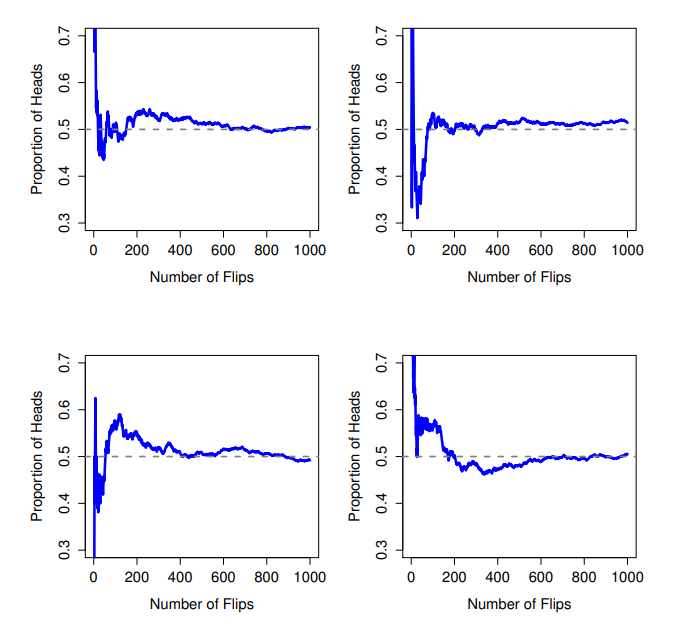
\includegraphics{./images/fig7-1.png} \hfill{}

\caption{\label{fig-fig7-1}An illustration of how frequentist
probability works. If you flip a fair coin over and over again the
proportion of heads that you've seen eventually settles down and
converges to the true probability of \(0.5\). Each panel shows four
different simulated experiments. In each case we pretend we flipped a
coin \(1000\) times and kept track of the proportion of flips that were
heads as we went along. Although none of these sequences actually ended
up with an exact value of \(.5\), if we'd extended the experiment for an
infinite number of coin flips they would have}

\end{figure}

\hypertarget{the-bayesian-view}{%
\subsection{The Bayesian view}\label{the-bayesian-view}}

\textbf{The Bayesian view} of probability is often called the
subjectivist view, and although it has been a minority view among
statisticians it has been steadily gaining traction for the last several
decades. There are many flavours of Bayesianism, making it hard to say
exactly what ``the'' Bayesian view is. The most common way of thinking
about subjective probability is to define the probability of an event as
the \textbf{degree of belief} that an intelligent and rational agent
assigns to that truth of that event. From that perspective,
probabilities don't exist in the world but rather in the thoughts and
assumptions of people and other intelligent beings.

However, in order for this approach to work we need some way of
operationalising ``degree of belief''. One way that you can do this is
to formalise it in terms of ``rational gambling'', though there are many
other ways. Suppose that I believe that there's a 60\% probability of
rain tomorrow. If someone offers me a bet that if it rains tomorrow then
I win \$5, but if it doesn't rain I lose \$5. Clearly, from my
perspective, this is a pretty good bet. On the other hand, if I think
that the probability of rain is only 40\% then it's a bad bet to take.
So we can operationalise the notion of a ``subjective probability'' in
terms of what bets I'm willing to accept.

What are the advantages and disadvantages to the Bayesian approach? The
main advantage is that it allows you to assign probabilities to any
event you want to. You don't need to be limited to those events that are
repeatable. The main disadvantage (to many people) is that we can't be
purely objective. Specifying a probability requires us to specify an
entity that has the relevant degree of belief. This entity might be a
human, an alien, a robot, or even a statistician. But there has to be an
intelligent agent out there that believes in things. To many people this
is uncomfortable, it seems to make probability arbitrary. Whilst the
Bayesian approach requires that the agent in question be rational (i.e.,
obey the rules of probability), it does allow everyone to have their own
beliefs. I can believe the coin is fair and you don't have to, even
though we're both rational. The frequentist view doesn't allow any two
observers to attribute different probabilities to the same event. When
that happens then at least one of them must be wrong. The Bayesian view
does not prevent this from occurring. Two observers with different
background knowledge can legitimately hold different beliefs about the
same event. In short, where the frequentist view is sometimes considered
to be too narrow (forbids lots of things that that we want to assign
probabilities to), the Bayesian view is sometimes thought to be too
broad (allows too many differences between observers).

\hypertarget{whats-the-difference-and-who-is-right}{%
\subsection{What's the difference? And who is
right?}\label{whats-the-difference-and-who-is-right}}

Now that you've seen each of these two views independently it's useful
to make sure you can compare the two. Go back to the hypothetical robot
soccer game at the start of the section. What do you think a frequentist
and a Bayesian would say about these three statements? Which statement
would a frequentist say is the correct definition of probability? Which
one would a Bayesian opt for? Would some of these statements be
meaningless to a frequentist or a Bayesian? If you've understood the two
perspectives you should have some sense of how to answer those
questions.

Okay, assuming you understand the difference then you might be wondering
which of them is \emph{right}? Honestly, I don't know that there is a
right answer. As far as I can tell there's nothing mathematically
incorrect about the way frequentists think about sequences of events,
and there's nothing mathematically incorrect about the way that
Bayesians define the beliefs of a rational agent. In fact, when you dig
down into the details Bayesians and frequentists actually agree about a
lot of things. Many frequentist methods lead to decisions that Bayesians
agree a rational agent would make. Many Bayesian methods have very good
frequentist properties.

For the most part, I'm a pragmatist so I'll use any statistical method
that I trust. As it turns out, that makes me prefer Bayesian methods for
reasons I'll explain towards the end of the book. But I'm not
fundamentally opposed to frequentist methods. Not everyone is quite so
relaxed. For instance, consider Sir Ronald Fisher, one of the towering
figures of 20th century statistics and a vehement opponent to all things
Bayesian, whose paper on the mathematical foundations of statistics
referred to Bayesian probability as ``an impenetrable jungle {[}that{]}
arrests progress towards precision of statistical concepts'' (Fisher,
1922b, p. 311). Or the psychologist Paul Meehl, who suggests that
relying on frequentist methods could turn you into ``a potent but
sterile intellectual rake who leaves in his merry path a long train of
ravished maidens but no viable scientific offspring'' (Meehl, 1967, p.
114). The history of statistics, as you might gather, is not devoid of
entertainment.

In any case, whilst I personally prefer the Bayesian view, the majority
of statistical analyses are based on the frequentist approach. My
reasoning is pragmatic. The goal of this book is to cover roughly the
same territory as a typical undergraduate stats class in psychology, and
if you want to understand the statistical tools used by most
psychologists you'll need a good grasp of frequentist methods. I promise
you that this isn't wasted effort. Even if you end up wanting to switch
to the Bayesian perspective, you really should read through at least one
book on the ``orthodox'' frequentist view. Besides, I won't completely
ignore the Bayesian perspective. Every now and then I'll add some
commentary from a Bayesian point of view, and I'll revisit the topic in
more depth in Chapter~\ref{sec-Bayesian-statistics}.

\hypertarget{basic-probability-theory}{%
\section{Basic probability theory}\label{basic-probability-theory}}

Ideological arguments between Bayesians and frequentists
notwithstanding, it turns out that people mostly agree on the rules that
probabilities should obey. There are lots of different ways of arriving
at these rules. The most commonly used approach is based on the work of
Andrey Kolmogorov, one of the great Soviet mathematicians of the 20th
century. I won't go into a lot of detail, but I'll try to give you a bit
of a sense of how it works. And in order to do so I'm going to have to
talk about my trousers.

\hypertarget{introducing-probability-distributions}{%
\subsection{Introducing probability
distributions}\label{introducing-probability-distributions}}

One of the disturbing truths about my life is that I only own 5 pairs of
trousers. Three pairs of jeans, the bottom half of a suit, and a pair of
tracksuit pants. Even sadder, I've given them names: I call them
\(X_1\), \(X_2\), \(X_3\), \(X_4\) and \(X_5\). I really have, that's
why they call me Mister Imaginative. Now, on any given day, I pick out
exactly one of pair of trousers to wear. Not even I'm so stupid as to
try to wear two pairs of trousers, and thanks to years of training I
never go outside without wearing trousers anymore. If I were to describe
this situation using the language of probability theory, I would refer
to each pair of trousers (i.e., each \(X\)) as an elementary event. The
key characteristic of \textbf{elementary events} is that every time we
make an observation (e.g., every time I put on a pair of trousers) then
the outcome will be one and only one of these events. Like I said, these
days I always wear exactly one pair of trousers so my trousers satisfy
this constraint. Similarly, the set of all possible events is called a
\textbf{sample space}. Granted, some people would call it a
``wardrobe'', but that's because they're refusing to think about my
trousers in probabilistic terms. Sad.

Okay, now that we have a sample space (a wardrobe), which is built from
lots of possible elementary events (trousers), what we want to do is
assign a \textbf{probability} of one of these elementary events. For an
event \(X\), the probability of that event \(P(X)\) is a number that
lies between 0 and 1. The bigger the value of \(P(X)\), the more likely
the event is to occur. So, for example, if \(P(X) = 0\) it means the
event \(X\) is impossible (i.e., I never wear those trousers). On the
other hand, if \(P(X) = 1\) it means that event \(X\) is certain to
occur (i.e., I always wear those trousers). For probability values in
the middle it means that I sometimes wear those trousers. For instance,
if \(P(X) = 0.5\) it means that I wear those trousers half of the time.

At this point, we're almost done. The last thing we need to recognise is
that ``something always happens''. Every time I put on trousers, I
really do end up wearing trousers (crazy, right?). What this somewhat
trite statement means, in probabilistic terms, is that the probabilities
of the elementary events need to add up to 1. This is known as the
\textbf{law of total probability}, not that any of us really care. More
importantly, if these requirements are satisfied then what we have is a
\textbf{probability distribution}. For example, Table~\ref{tbl-tab7-2}
shows an example of a probability distribution.

\hypertarget{tbl-tab7-2}{}
 
  \providecommand{\huxb}[2]{\arrayrulecolor[RGB]{#1}\global\arrayrulewidth=#2pt}
  \providecommand{\huxvb}[2]{\color[RGB]{#1}\vrule width #2pt}
  \providecommand{\huxtpad}[1]{\rule{0pt}{#1}}
  \providecommand{\huxbpad}[1]{\rule[-#1]{0pt}{#1}}

\begin{table}[ht]
\caption{\label{tbl-tab7-2}A probability distribution for trouser wearing }\tabularnewline

\begin{centerbox}
\begin{threeparttable}
\setlength{\tabcolsep}{0pt}
\begin{tabularx}{0.9\textwidth}{p{0.3\textwidth} p{0.3\textwidth} p{0.3\textwidth}}


\hhline{>{\huxb{0, 0, 0}{0.4}}->{\huxb{0, 0, 0}{0.4}}->{\huxb{0, 0, 0}{0.4}}-}
\arrayrulecolor{black}

\multicolumn{1}{!{\huxvb{0, 0, 0}{0}}p{0.3\textwidth}!{\huxvb{0, 0, 0}{0}}}{\cellcolor[RGB]{242, 242, 242}\hspace{0pt}\parbox[b]{0.3\textwidth-0pt-6pt}{\huxtpad{6pt + 1em}\centering \textbf{Which trousers?}\huxbpad{6pt}}} &
\multicolumn{1}{p{0.3\textwidth}!{\huxvb{0, 0, 0}{0}}}{\cellcolor[RGB]{242, 242, 242}\hspace{6pt}\parbox[b]{0.3\textwidth-6pt-6pt}{\huxtpad{6pt + 1em}\centering \textbf{Label}\huxbpad{6pt}}} &
\multicolumn{1}{p{0.3\textwidth}!{\huxvb{0, 0, 0}{0}}}{\cellcolor[RGB]{242, 242, 242}\hspace{6pt}\parbox[b]{0.3\textwidth-6pt-0pt}{\huxtpad{6pt + 1em}\centering \textbf{Probability}\huxbpad{6pt}}} \tabularnewline[-0.5pt]


\hhline{>{\huxb{0, 0, 0}{0.4}}->{\huxb{0, 0, 0}{0.4}}->{\huxb{0, 0, 0}{0.4}}-}
\arrayrulecolor{black}

\multicolumn{1}{!{\huxvb{0, 0, 0}{0}}p{0.3\textwidth}!{\huxvb{0, 0, 0}{0}}}{\hspace{0pt}\parbox[b]{0.3\textwidth-0pt-6pt}{\huxtpad{6pt + 1em}\centering Blue jeans\huxbpad{6pt}}} &
\multicolumn{1}{p{0.3\textwidth}!{\huxvb{0, 0, 0}{0}}}{\hspace{6pt}\parbox[b]{0.3\textwidth-6pt-6pt}{\huxtpad{6pt + 1em}\centering \(X_1 \)\huxbpad{6pt}}} &
\multicolumn{1}{p{0.3\textwidth}!{\huxvb{0, 0, 0}{0}}}{\hspace{6pt}\parbox[b]{0.3\textwidth-6pt-0pt}{\huxtpad{6pt + 1em}\centering \(P(X_1)=.5 \)\huxbpad{6pt}}} \tabularnewline[-0.5pt]


\hhline{}
\arrayrulecolor{black}

\multicolumn{1}{!{\huxvb{0, 0, 0}{0}}p{0.3\textwidth}!{\huxvb{0, 0, 0}{0}}}{\cellcolor[RGB]{242, 242, 242}\hspace{0pt}\parbox[b]{0.3\textwidth-0pt-6pt}{\huxtpad{6pt + 1em}\centering Grey jeans\huxbpad{6pt}}} &
\multicolumn{1}{p{0.3\textwidth}!{\huxvb{0, 0, 0}{0}}}{\cellcolor[RGB]{242, 242, 242}\hspace{6pt}\parbox[b]{0.3\textwidth-6pt-6pt}{\huxtpad{6pt + 1em}\centering \(X_2 \)\huxbpad{6pt}}} &
\multicolumn{1}{p{0.3\textwidth}!{\huxvb{0, 0, 0}{0}}}{\cellcolor[RGB]{242, 242, 242}\hspace{6pt}\parbox[b]{0.3\textwidth-6pt-0pt}{\huxtpad{6pt + 1em}\centering \(P(X_2)=.3 \)\huxbpad{6pt}}} \tabularnewline[-0.5pt]


\hhline{}
\arrayrulecolor{black}

\multicolumn{1}{!{\huxvb{0, 0, 0}{0}}p{0.3\textwidth}!{\huxvb{0, 0, 0}{0}}}{\hspace{0pt}\parbox[b]{0.3\textwidth-0pt-6pt}{\huxtpad{6pt + 1em}\centering Black jeans\huxbpad{6pt}}} &
\multicolumn{1}{p{0.3\textwidth}!{\huxvb{0, 0, 0}{0}}}{\hspace{6pt}\parbox[b]{0.3\textwidth-6pt-6pt}{\huxtpad{6pt + 1em}\centering \(X_3 \)\huxbpad{6pt}}} &
\multicolumn{1}{p{0.3\textwidth}!{\huxvb{0, 0, 0}{0}}}{\hspace{6pt}\parbox[b]{0.3\textwidth-6pt-0pt}{\huxtpad{6pt + 1em}\centering \(P(X_3)=.1 \)\huxbpad{6pt}}} \tabularnewline[-0.5pt]


\hhline{}
\arrayrulecolor{black}

\multicolumn{1}{!{\huxvb{0, 0, 0}{0}}p{0.3\textwidth}!{\huxvb{0, 0, 0}{0}}}{\cellcolor[RGB]{242, 242, 242}\hspace{0pt}\parbox[b]{0.3\textwidth-0pt-6pt}{\huxtpad{6pt + 1em}\centering Black suit\huxbpad{6pt}}} &
\multicolumn{1}{p{0.3\textwidth}!{\huxvb{0, 0, 0}{0}}}{\cellcolor[RGB]{242, 242, 242}\hspace{6pt}\parbox[b]{0.3\textwidth-6pt-6pt}{\huxtpad{6pt + 1em}\centering \(X_4 \)\huxbpad{6pt}}} &
\multicolumn{1}{p{0.3\textwidth}!{\huxvb{0, 0, 0}{0}}}{\cellcolor[RGB]{242, 242, 242}\hspace{6pt}\parbox[b]{0.3\textwidth-6pt-0pt}{\huxtpad{6pt + 1em}\centering \(P(X_4)=0 \)\huxbpad{6pt}}} \tabularnewline[-0.5pt]


\hhline{}
\arrayrulecolor{black}

\multicolumn{1}{!{\huxvb{0, 0, 0}{0}}p{0.3\textwidth}!{\huxvb{0, 0, 0}{0}}}{\hspace{0pt}\parbox[b]{0.3\textwidth-0pt-6pt}{\huxtpad{6pt + 1em}\centering Blue tracksuit\huxbpad{6pt}}} &
\multicolumn{1}{p{0.3\textwidth}!{\huxvb{0, 0, 0}{0}}}{\hspace{6pt}\parbox[b]{0.3\textwidth-6pt-6pt}{\huxtpad{6pt + 1em}\centering \(X_5 \)\huxbpad{6pt}}} &
\multicolumn{1}{p{0.3\textwidth}!{\huxvb{0, 0, 0}{0}}}{\hspace{6pt}\parbox[b]{0.3\textwidth-6pt-0pt}{\huxtpad{6pt + 1em}\centering \(P(X_5)=.1 \)\huxbpad{6pt}}} \tabularnewline[-0.5pt]


\hhline{>{\huxb{0, 0, 0}{0.4}}->{\huxb{0, 0, 0}{0.4}}->{\huxb{0, 0, 0}{0.4}}-}
\arrayrulecolor{black}
\end{tabularx} 

\end{threeparttable}\par\end{centerbox}

\end{table}
 

Each of the events has a probability that lies between 0 and 1, and if
we add up the probability of all events they sum to 1. Awesome. We can
even draw a nice bar graph (see Section~\ref{sec-Bar-graphs}) to
visualise this distribution, as shown in Figure~\ref{fig-fig7-2}. And,
at this point, we've all achieved something. You've learned what a
probability distribution is, and I've finally managed to find a way to
create a graph that focuses entirely on my trousers. Everyone wins! The
only other thing that I need to point out is that probability theory
allows you to talk about \textbf{non elementary events} as well as
elementary ones. The easiest way to illustrate the concept is with an
example. In the trousers example it's perfectly legitimate to refer to
the probability that I wear jeans. In this scenario, the ``Dani wears
jeans'' event is said to have happened as long as the elementary event
that actually did occur is one of the appropriate ones. In this case
``blue jeans'', ``black jeans'' or ``grey jeans''. In mathematical terms
we defined the ``jeans'' event \(E\) to correspond to the set of
elementary events \((X1, X2, X3)\). If any of these elementary events
occurs then \(E\) is also said to have occurred. Having decided to write
down the definition of the E this way, it's pretty straightforward to
state what the probability P(E) and, since the probabilities of blue,
grey and black jeans respectively are \(.5\), \(.3\) and \(.1\), the
probability that I wear jeans is equal to \(.9\). is: we just add
everything up. In this particular case \[P(E)=P(X_1)+P(X_2)+P(X_3)\] At
this point you might be thinking that this is all terribly obvious and
simple and you'd be right. All we've really done is wrap some basic
mathematics around a few common sense intuitions. However, from these
simple beginnings it's possible to construct some extremely powerful
mathematical tools. I'm definitely not going to go into the details in
this book, but what I will do is list, in Table~\ref{tbl-tab7-3}, some
of the other rules that probabilities satisfy. These rules can be
derived from the simple assumptions that I've outlined above, but since
we don't actually use these rules for anything in this book I won't do
so here.

\begin{figure}

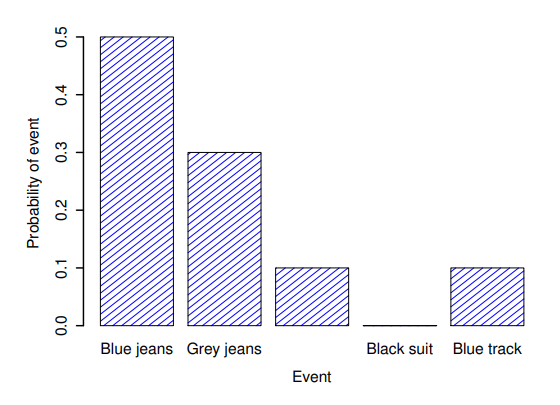
\includegraphics{./images/fig7-2.png} \hfill{}

\caption{\label{fig-fig7-2}A visual depiction of the `trousers'
probability distribution. There are five `elementary events',
corresponding to the five pairs of trousers that I own. Each event has
some probability of occurring - this probability is a number between 0
to 1. The sum of these probabilities is 1}

\end{figure}

\hypertarget{tbl-tab7-3}{}
 
  \providecommand{\huxb}[2]{\arrayrulecolor[RGB]{#1}\global\arrayrulewidth=#2pt}
  \providecommand{\huxvb}[2]{\color[RGB]{#1}\vrule width #2pt}
  \providecommand{\huxtpad}[1]{\rule{0pt}{#1}}
  \providecommand{\huxbpad}[1]{\rule[-#1]{0pt}{#1}}

\begin{table}[ht]
\caption{\label{tbl-tab7-3}Some rules that probabilities satisfy }\tabularnewline

\begin{centerbox}
\begin{threeparttable}
\setlength{\tabcolsep}{0pt}
\begin{tabularx}{0.9\textwidth}{p{0.3\textwidth} p{0.3\textwidth} p{0.3\textwidth}}


\hhline{>{\huxb{0, 0, 0}{0.4}}->{\huxb{0, 0, 0}{0.4}}->{\huxb{0, 0, 0}{0.4}}-}
\arrayrulecolor{black}

\multicolumn{1}{!{\huxvb{0, 0, 0}{0}}p{0.3\textwidth}!{\huxvb{0, 0, 0}{0}}}{\cellcolor[RGB]{242, 242, 242}\hspace{0pt}\parbox[b]{0.3\textwidth-0pt-6pt}{\huxtpad{6pt + 1em}\centering \textbf{English}\huxbpad{6pt}}} &
\multicolumn{1}{p{0.3\textwidth}!{\huxvb{0, 0, 0}{0}}}{\cellcolor[RGB]{242, 242, 242}\hspace{6pt}\parbox[b]{0.3\textwidth-6pt-6pt}{\huxtpad{6pt + 1em}\centering \textbf{Notation}\huxbpad{6pt}}} &
\multicolumn{1}{p{0.3\textwidth}!{\huxvb{0, 0, 0}{0}}}{\cellcolor[RGB]{242, 242, 242}\hspace{6pt}\parbox[b]{0.3\textwidth-6pt-0pt}{\huxtpad{6pt + 1em}\centering \textbf{Formula}\huxbpad{6pt}}} \tabularnewline[-0.5pt]


\hhline{>{\huxb{0, 0, 0}{0.4}}->{\huxb{0, 0, 0}{0.4}}->{\huxb{0, 0, 0}{0.4}}-}
\arrayrulecolor{black}

\multicolumn{1}{!{\huxvb{0, 0, 0}{0}}p{0.3\textwidth}!{\huxvb{0, 0, 0}{0}}}{\hspace{0pt}\parbox[b]{0.3\textwidth-0pt-6pt}{\huxtpad{6pt + 1em}\centering not A\huxbpad{6pt}}} &
\multicolumn{1}{p{0.3\textwidth}!{\huxvb{0, 0, 0}{0}}}{\hspace{6pt}\parbox[b]{0.3\textwidth-6pt-6pt}{\huxtpad{6pt + 1em}\centering \(P (\neg A) \)\huxbpad{6pt}}} &
\multicolumn{1}{p{0.3\textwidth}!{\huxvb{0, 0, 0}{0}}}{\hspace{6pt}\parbox[b]{0.3\textwidth-6pt-0pt}{\huxtpad{6pt + 1em}\centering \(1-P(A) \)\huxbpad{6pt}}} \tabularnewline[-0.5pt]


\hhline{}
\arrayrulecolor{black}

\multicolumn{1}{!{\huxvb{0, 0, 0}{0}}p{0.3\textwidth}!{\huxvb{0, 0, 0}{0}}}{\cellcolor[RGB]{242, 242, 242}\hspace{0pt}\parbox[b]{0.3\textwidth-0pt-6pt}{\huxtpad{6pt + 1em}\centering A or B\huxbpad{6pt}}} &
\multicolumn{1}{p{0.3\textwidth}!{\huxvb{0, 0, 0}{0}}}{\cellcolor[RGB]{242, 242, 242}\hspace{6pt}\parbox[b]{0.3\textwidth-6pt-6pt}{\huxtpad{6pt + 1em}\centering \(P(A \cup B) \)\huxbpad{6pt}}} &
\multicolumn{1}{p{0.3\textwidth}!{\huxvb{0, 0, 0}{0}}}{\cellcolor[RGB]{242, 242, 242}\hspace{6pt}\parbox[b]{0.3\textwidth-6pt-0pt}{\huxtpad{6pt + 1em}\centering \(P(A) + P(B) - P(A \cap B) \)\huxbpad{6pt}}} \tabularnewline[-0.5pt]


\hhline{}
\arrayrulecolor{black}

\multicolumn{1}{!{\huxvb{0, 0, 0}{0}}p{0.3\textwidth}!{\huxvb{0, 0, 0}{0}}}{\hspace{0pt}\parbox[b]{0.3\textwidth-0pt-6pt}{\huxtpad{6pt + 1em}\centering A and B\huxbpad{6pt}}} &
\multicolumn{1}{p{0.3\textwidth}!{\huxvb{0, 0, 0}{0}}}{\hspace{6pt}\parbox[b]{0.3\textwidth-6pt-6pt}{\huxtpad{6pt + 1em}\centering \(P(A \cap B) \)\huxbpad{6pt}}} &
\multicolumn{1}{p{0.3\textwidth}!{\huxvb{0, 0, 0}{0}}}{\hspace{6pt}\parbox[b]{0.3\textwidth-6pt-0pt}{\huxtpad{6pt + 1em}\centering \(P(A|B) P(B) \)\huxbpad{6pt}}} \tabularnewline[-0.5pt]


\hhline{>{\huxb{0, 0, 0}{0.4}}->{\huxb{0, 0, 0}{0.4}}->{\huxb{0, 0, 0}{0.4}}-}
\arrayrulecolor{black}
\end{tabularx} 

\end{threeparttable}\par\end{centerbox}

\end{table}
 

\hypertarget{sec-The-binomial-distribution}{%
\section{The binomial
distribution}\label{sec-The-binomial-distribution}}

As you might imagine, probability distributions vary enormously and
there's an enormous range of distributions out there. However, they
aren't all equally important. In fact, the vast majority of the content
in this book relies on one of five distributions: the binomial
distribution, the normal distribution, the t distribution, the
\(\chi^2\) (``chi-square'') distribution and the F distribution. Given
this, what I'll do over the next few sections is provide a brief
introduction to all five of these, paying special attention to the
binomial and the normal. I'll start with the binomial distribution since
it's the simplest of the five.

\hypertarget{introducing-the-binomial}{%
\subsection{Introducing the binomial}\label{introducing-the-binomial}}

The theory of probability originated in the attempt to describe how
games of chance work, so it seems fitting that our discussion of the
\textbf{binomial distribution} should involve a discussion of rolling
dice and flipping coins. Let's imagine a simple ``experiment''. In my
hot little hand I'm holding 20 identical six-sided dice. On one face of
each die there's a picture of a skull, the other five faces are all
blank. If I proceed to roll all 20 dice, what's the probability that
I'll get exactly 4 skulls? Assuming that the dice are fair, we know that
the chance of any one die coming up skulls is 1 in 6. To say this
another way, the skull probability for a single die is approximately
.167. This is enough information to answer our question, so let's have a
look at how it's done.

As usual, we'll want to introduce some names and some notation. We'll
let \(N\) denote the number of dice rolls in our experiment, which is
often referred to as the \textbf{size parameter} of our binomial
distribution. We'll also use \(\theta\) to refer to the the probability
that a single die comes up skulls, a quantity that is usually called the
\textbf{success probability} of the binomial.\footnote{Note that the
  term ``success'' is pretty arbitrary and doesn't actually imply that
  the outcome is something to be desired. If \(\theta\) referred to the
  probability that any one passenger gets injured in a bus crash I'd
  still call it the success probability, but that doesn't mean I want
  people to get hurt in bus crashes!} Finally, we'll use \(X\) to refer
to the results of our experiment, namely the number of skulls I get when
I roll the dice. Since the actual value of \(X\) is due to chance we
refer to it as a \textbf{random variable}. In any case, now that we have
all this terminology and notation we can use it to state the problem a
little more precisely. The quantity that we want to calculate is the
probability that \(X = 4\) given that we know that \(\theta = .167\) and
\(N = 20\). The general ``form'' of the thing I'm interested in
calculating could be written as

\[P(X|\theta,N)\]

and we're interested in the special case where \$X = 4, \theta = .167 \$
and \(N = 20\).

{[}Additional technical detail \footnote{For those readers who know a
  little calculus, I'll give a slightly more precise explanation. In the
  same way that probabilities are non-negative numbers that must sum to
  1, probability densities are non-negative numbers that must integrate
  to 1 (where the integral is taken across all possible values of X). To
  calculate the probability that X falls between a and b we calculate
  the definite integral of the density function over the corresponding
  range, \(\int\_{a}^{b} p(x) dx\). If you don't remember or never
  learned calculus, don't worry about this. It's not needed for this
  book.}{]}

Yeah, yeah. I know what you're thinking: notation, notation, notation.
Really, who cares? Very few readers of this book are here for the
notation, so I should probably move on and talk about how to use the
binomial distribution. I've included the formula for the binomial
distribution in Table~\ref{tbl-tab7-2}, since some readers may want to
play with it themselves, but since most people probably don't care that
much and because we don't need the formula in this book, I won't talk
about it in any detail. Instead, I just want to show you what the
binomial distribution looks like.

To that end, Figure~\ref{fig-fig7-3} plots the binomial probabilities
for all possible values of \(X\) for our dice rolling experiment, from
\(X = 0\) (no skulls) all the way up to \(X = 20\) (all skulls). Note
that this is basically a bar chart, and is no different to the
``trousers probability'' plot I drew in Figure~\ref{fig-fig7-2}. On the
horizontal axis we have all the possible events, and on the vertical
axis we can read off the probability of each of those events. So, the
probability of rolling \(4\) skulls out of \(20\) is about \(0.20\) (the
actual answer is \(0.2022036\), as we'll see in a moment). In other
words, you'd expect that to happen about 20\% of the times you repeated
this experiment.

To give you a feel for how the binomial distribution changes when we
alter the values of \(theta\) and \(N\), let's suppose that instead of
rolling dice I'm actually flipping coins. This time around, my
experiment involves flipping a fair coin repeatedly and the outcome that
I'm interested in is the number of heads that I observe. In this
scenario, the success probability is now \(\theta = \frac{1}{2}\).
Suppose I were to flip the coin \(N = 20\) times. In this example, I've
changed the success probability but kept the size of the experiment the
same. What does this do to our binomial distribution? Well, as
Figure~\ref{fig-fig7-4} shows, the main effect of this is to shift the
whole distribution, as you'd expect. Okay, what if we flipped a coin
\(N = 100\) times? Well, in that case we get Figure~\ref{fig-fig7-4}
(b). The distribution stays roughly in the middle but there's a bit more
variability in the possible outcomes.

\begin{figure}

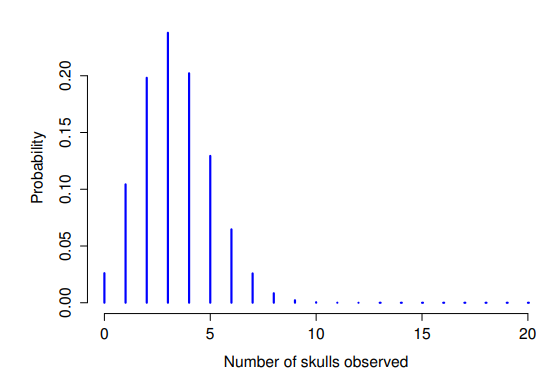
\includegraphics{./images/fig7-3.png} \hfill{}

\caption{\label{fig-fig7-3}The binomial distribution with size parameter
of \(N = 20\) and an underlying success probability of
\(\theta = \frac{1}{6}\). Each vertical bar depicts the probability of
one specific outcome (i.e., one possible value of X). Because this is a
probability distribution, each of the probabilities must be a number
between 0 and 1, and the heights of the bars must sum to 1 as well}

\end{figure}

I were to flip the coin \(N = 20\) times. In this example, I've changed
the success probability but kept the size of the experiment the same.
What does this do to our binomial distribution? Well, as
Figure~\ref{fig-fig7-4} (a) shows, the main effect of this is to shift
the whole distribution, as you'd expect. Okay, what if we flipped a coin
\(N = 100\) times? Well, in that case we get Figure~\ref{fig-fig7-4}
(a). The distribution stays roughly in the middle but there's a bit more
variability in the possible outcomes.

\hypertarget{sec-The-normal-distribution}{%
\section{The normal distribution}\label{sec-The-normal-distribution}}

While the binomial distribution is conceptually the simplest
distribution to understand, it's not the most important one. That
particular honour goes to the normal distribution, also referred to as
``the bell curve'' or a ``Gaussian distribution''. A \textbf{normal
distribution} is described using two parameters: the mean of the
distribution µ and the standard deviation of the distribution
\(\sigma\).

\begin{figure}

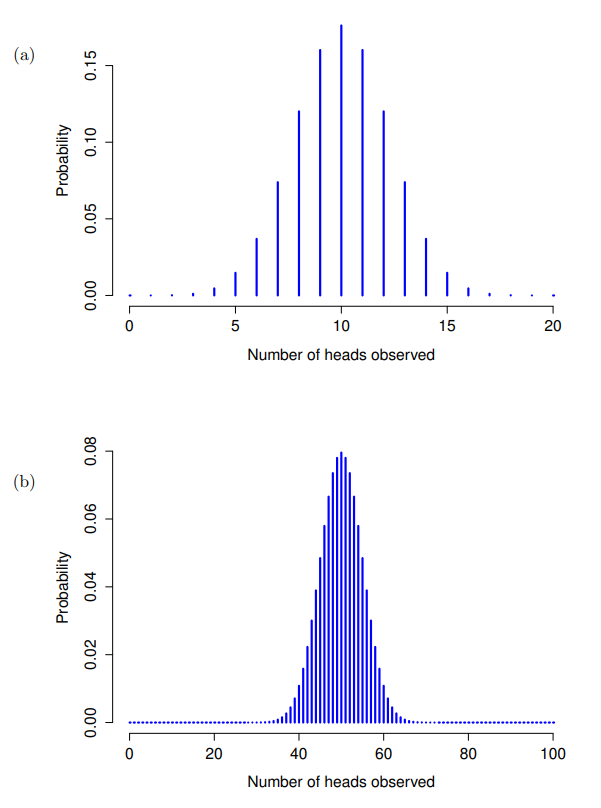
\includegraphics{./images/fig7-4.png} \hfill{}

\caption{\label{fig-fig7-4}Two binomial distributions, involving a
scenario in which I'm flipping a fair coin, so the underlying success
probability is \(\theta = \frac{1}{2}\). In panel (a), we assume I'm
flipping the coin \(N = 20\) times. In panel (b) we assume that the coin
is flipped \(N = 100\) times}

\end{figure}

\begin{figure}

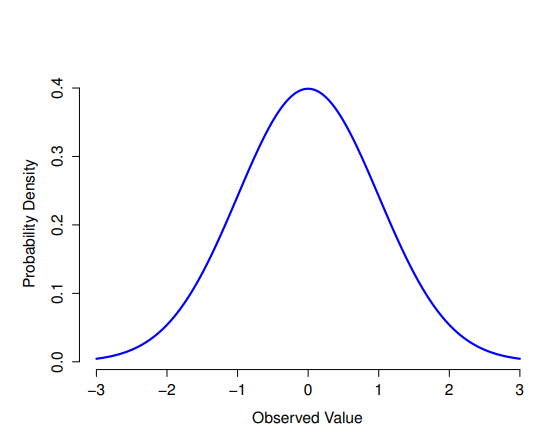
\includegraphics{./images/fig7-5.png} \hfill{}

\caption{\label{fig-fig7-5}The normal distribution with mean \(\mu = 0\)
and standard deviation \(\sigma = 1\). The x-axis corresponds to the
value of some variable, and the y-axis tells us something about how
likely we are to observe that value. However, notice that the y-axis is
labelled \emph{Probability Density} and not \emph{Probability}. There is
a subtle and somewhat frustrating characteristic of continuous
distributions that makes the \(y\) axis behave a bit oddly - the height
of the curve here isn't actually the probability of observing a
particular x value. On the other hand, it is true that the heights of
the curve tells you which \(x\) values are more likely (the higher
ones!). (see \protect\hyperlink{probability-density}{Probability
density} section for all the annoying details)}

\end{figure}

{[}Additional technical detail \footnote{The notation that we sometimes
  use to say that a variable \(X\) is normally distributed is as
  follows: \[X \sim Normal(\mu,\sigma)\] Of course, that's just
  notation. It doesn't tell us anything interesting about the normal
  distribution itself. As was the case with the binomial distribution, I
  have included the formula for the normal distribution in this book,
  because I think it's important enough that everyone who learns
  statistics should at least look at it, but since this is an
  introductory text I don't want to focus on it, so I've tucked it away
  in this footnote.}{]}

Let's try to get a sense for what it means for a variable to be normally
distributed. To that end, have a look at Figure~\ref{fig-fig7-5} which
plots a normal distribution with mean \(\mu = 0\) and standard deviation
\(\sigma = 1\). You can see where the name ``bell curve'' comes from; it
looks a bit like a bell. Notice that, unlike the plots that I drew to
illustrate the binomial distribution, the picture of the normal
distribution in Figure~\ref{fig-fig7-5} shows a smooth curve instead of
``histogram-like'' bars. This isn't an arbitrary choice, the normal
distribution is continuous whereas the binomial is discrete. For
instance, in the die rolling example from the last section it was
possible to get 3 skulls or 4 skulls, but impossible to get 3.9 skulls.
The figures that I drew in the previous section reflected this fact. In
Figure~\ref{fig-fig7-3}, for instance, there's a bar located at
\(X = 3\) and another one at \(X = 4\) but there's nothing in between.
Continuous quantities don't have this constraint. For instance, suppose
we're talking about the weather. The temperature on a pleasant Spring
day could be 23 degrees, 24 degrees, 23.9 degrees, or anything in
between since temperature is a continuous variable. And so a normal
distribution might be quite appropriate for describing Spring
temperatures\footnote{In practice, the normal distribution is so handy
  that people tend to use it even when the variable isn't actually
  continuous. As long as there are enough categories (e.g., Likert scale
  responses to a questionnaire), it's pretty standard practice to use
  the normal distribution as an approximation. This works out much
  better in practice than you'd think.}

\begin{figure}

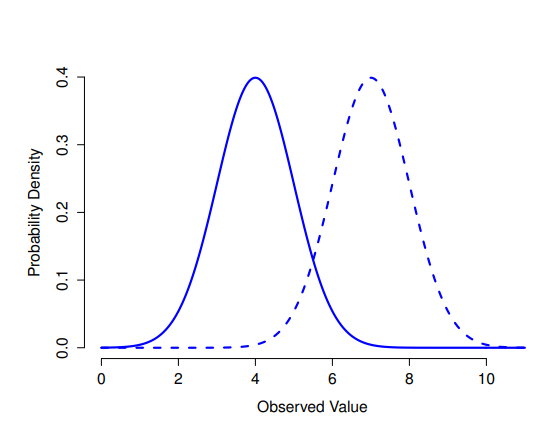
\includegraphics{./images/fig7-6.png} \hfill{}

\caption{\label{fig-fig7-6}An illustration of what happens when you
change the mean of a normal distribution. The solid line depicts a
normal distribution with a mean of \(\mu = 4\). The dashed line shows a
normal distribution with a mean of \(\mu = 7\). In both cases, the
standard deviation is \(\sigma = 1\). Not surprisingly, the two
distributions have the same shape, but the dashed line is shifted to the
right}

\end{figure}

With this in mind, let's see if we can't get an intuition for how the
normal distribution works. First, let's have a look at what happens when
we play around with the parameters of the distribution. To that end,
Figure~\ref{fig-fig7-6} plots normal distributions that have different
means but have the same standard deviation. As you might expect, all of
these distributions have the same ``width''. The only difference between
them is that they've been shifted to the left or to the right. In every
other respect they're identical. In contrast, if we increase the
standard deviation while keeping the mean constant, the peak of the
distribution stays in the same place but the distribution gets wider, as
you can see in Figure~\ref{fig-fig7-7}. Notice, though, that when we
widen the distribution the height of the peak shrinks. This has to
happen, in the same way that the heights of the bars that we used to
draw a discrete binomial distribution have to sum to 1, the total area
under the curve for the normal distribution must equal 1. Before moving
on, I want to point out one important characteristic of the normal
distribution. Irrespective of what the actual mean and standard
deviation are, \(68.3\%\) of the area falls within 1 standard deviation
of the mean. Similarly, \(95.4\%\) of the distribution falls within 2
standard deviations of the mean, and \((99.7\%)\) of the distribution is
within 3 standard deviations. This idea is illustrated in
Figure~\ref{fig-fig7-8}; see also Figure~\ref{fig-fig7-9}.

\begin{figure}

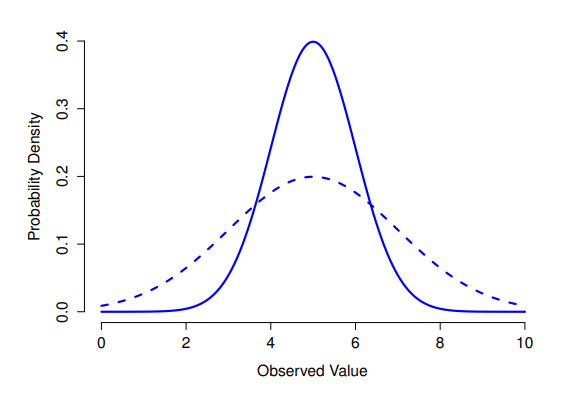
\includegraphics{./images/fig7-7.png} \hfill{}

\caption{\label{fig-fig7-7}An illustration of what happens when you
change the the standard deviation of a normal distribution. Both
distributions plotted in this figure have a mean of \(\mu = 5\), but
they have different standard deviations. The solid line plots a
distribution with standard deviation \(\sigma = 1\), and the dashed line
shows a distribution with standard deviation \(\sigma = 2\). As a
consequence, both distributions are `centred' on the same spot, but the
dashed line is wider than the solid one}

\end{figure}

\begin{figure}

\includegraphics{./images/fig7-8.png} \hfill{}

\caption{\label{fig-fig7-8}The area under the curve tells you the
probability that an observation falls within a particular range. The
solid lines plot normal distributions with mean \(\mu = 0\) and standard
deviation \(\sigma = 1\). The shaded areas illustrate `areas under the
curve' for two important cases. In panel (a), we can see that there is a
68.3\% chance that an observation will fall within one standard
deviation of the mean. In panel (b), we see that there is a 95.4\%
chance that an observation will fall within two standard deviations of
the mean}

\end{figure}

\begin{figure}

\includegraphics{./images/fig7-9.png} \hfill{}

\caption{\label{fig-fig7-9}Two more examples of the `area under the
curve idea'. There is a 15.9\% chance that an observation is one
standard deviation below the mean or smaller (panel (a)), and a 34.1\%
chance that the observation is somewhere between one standard deviation
below the mean and the mean (panel (b)). Notice that if you add these
two numbers together you get 15.9\% + 34.1\% = 50\%. For normally
distributed data, there is a 50\% chance that an observation falls below
the mean. And of course that also implies that there is a 50\% chance
that it falls above the mean}

\end{figure}

\hypertarget{probability-density}{%
\subsection{Probability density}\label{probability-density}}

There's something I've been trying to hide throughout my discussion of
the normal distribution, something that some introductory textbooks omit
completely. They might be right to do so. This ``thing'' that I'm hiding
is weird and counter-intuitive even by the admittedly distorted
standards that apply in statistics. Fortunately, it's not something that
you need to understand at a deep level in order to do basic statistics.
Rather, it's something that starts to become important later on when you
move beyond the basics. So, if it doesn't make complete sense, don't
worry too much, but try to make sure that you follow the gist of it.

Throughout my discussion of the normal distribution there's been one or
two things that don't quite make sense. Perhaps you noticed that the
y-axis in these figures is labelled ``Probability Density'' rather than
density. Maybe you noticed that I used \(P(X)\) instead of \(P(X)\) when
giving the formula for the normal distribution.

As it turns out, what is presented here isn't actually a probability,
it's something else. To understand what that something is you have to
spend a little time thinking about what it really means to say that
\(X\) is a continuous variable. Let's say we're talking about the
temperature outside. The thermometer tells me it's \(23\) degrees, but I
know that's not really true. It's not exactly \(23\) degrees. Maybe it's
\(23.1\) degrees, I think to myself. But I know that that's not really
true either because it might actually be \(23.09\) degrees. But I know
that\ldots{} well, you get the idea. The tricky thing with genuinely
continuous quantities is that you never really know exactly what they
are.

Now think about what this implies when we talk about probabilities.
Suppose that tomorrow's maximum temperature is sampled from a normal
distribution with mean \(23\) and standard deviation 1. What's the
probability that the temperature will be exactly \(23\) degrees? The
answer is ``zero'', or possibly ``a number so close to zero that it
might as well be zero''. Why is this? It's like trying to throw a dart
at an infinitely small dart board. No matter how good your aim, you'll
never hit it. In real life you'll never get a value of exactly \(23\).
It'll always be something like \(23.1\) or \(22.99998\) or suchlike. In
other words, it's completely meaningless to talk about the probability
that the temperature is exactly \(23\) degrees. However, in everyday
language if I told you that it was \(23\) degrees outside and it turned
out to be \(22.9998\) degrees you probably wouldn't call me a liar.
Because in everyday language ``\(23\) degrees'' usually means something
like ``somewhere between \(22.5\) and \(23.5\) degrees''. And while it
doesn't feel very meaningful to ask about the probability that the
temperature is exactly \(23\) degrees, it does seem sensible to ask
about the probability that the temperature lies between \(22.5\) and
\(23.5\), or between \(20\) and \(30\), or any other range of
temperatures.

The point of this discussion is to make clear that when we're talking
about continuous distributions it's not meaningful to talk about the
probability of a specific value. However, what we can talk about is the
probability that the value lies within a particular range of values. To
find out the probability associated with a particular range what you
need to do is calculate the ``area under the curve''. We've seen this
concept already, in Figure~\ref{fig-fig7-8} the shaded areas shown
depict genuine probabilities (e.g., in Figure~\ref{fig-fig7-8}) it shows
the probability of observing a value that falls within 1 standard
deviation of the mean).

Okay, so that explains part of the story. I've explained a little bit
about how continuous probability distributions should be interpreted
(i.e., area under the curve is the key thing). But what does the formula
for ppxq that I described earlier actually mean? Obviously, \(P(x)\)
doesn't describe a probability, but what is it? The name for this
quantity \(P(x)\) is a \textbf{probability density}, and in terms of the
plots we've been drawing it corresponds to the height of the curve. The
densities themselves aren't meaningful in and of themselves, but they're
``rigged'' to ensure that the area under the curve is always
interpretable as genuine probabilities. To be honest, that's about as
much as you really need to know for now.\footnote{For those readers who
  know a little calculus, I'll give a slightly more precise explanation.
  In the same way that probabilities are non-negative numbers that must
  sum to 1, probability densities are non-negative numbers that must
  integrate to 1 (where the integral is taken across all possible values
  of X). To calculate the probability that X falls between a and b we
  calculate the definite integral of the density function over the
  corresponding range, \(\int\_{a}^{b} p(x) dx\). If you don't remember
  or never learned calculus, don't worry about this. It's not needed for
  this book.}

\hypertarget{sec-Other-useful-distributions}{%
\section{Other useful
distributions}\label{sec-Other-useful-distributions}}

The normal distribution is the distribution that statistics makes most
use of (for reasons to be discussed shortly), and the binomial
distribution is a very useful one for lots of purposes. But the world of
statistics is filled with probability distributions, some of which we'll
run into in passing. In particular, the three that will appear in this
book are the t distribution, the \(\chi^2\) distribution and the F
distribution. I won't give formulas for any of these, or talk about them
in too much detail, but I will show you some pictures:
Figure~\ref{fig-fig7-10}, Figure~\ref{fig-fig7-11} and
Figure~\ref{fig-fig7-12}.

\begin{figure}

\includegraphics{./images/fig7-10.png} \hfill{}

\caption{\label{fig-fig7-10}A \(t\) distribution with 3 degrees of
freedom (solid line). It looks similar to a normal distribution, but
it's not quite the same. For comparison purposes I've plotted a standard
normal distribution as the dashed line}

\end{figure}

\begin{figure}

\includegraphics{./images/fig7-11.png} \hfill{}

\caption{\label{fig-fig7-11}\(\chi^2\) distribution with 3 degrees of
freedom. Notice that the observed values must always be greater than
zero, and that the distribution is pretty skewed. These are the key
features of a chi-square distribution}

\end{figure}

\begin{figure}

\includegraphics{./images/fig7-12.png} \hfill{}

\caption{\label{fig-fig7-12}An \(F\) distribution with 3 and 5 degrees
of freedom. Qualitatively speaking, it looks pretty similar to a
chi-square distribution, but they're not quite the same in general}

\end{figure}

\begin{itemize}
\tightlist
\item
  The \(t\) distribution is a continuous distribution that looks very
  similar to a normal distribution, see Figure~\ref{fig-fig7-10}. Note
  that the ``tails'' of the t distribution are ``heavier'' (i.e., extend
  further outwards) than the tails of the normal distribution). That's
  the important difference between the two. This distribution tends to
  arise in situations where you think that the data actually follow a
  normal distribution, but you don't know the mean or standard
  deviation. We'll run into this distribution again in
  Chapter~\ref{sec-Comparing-two-means}.
\item
  The \(\chi^2\) distribution is another distribution that turns up in
  lots of different places. The situation in which we'll see it is when
  doing categorical data analysis in
  Chapter~\ref{sec-Categorical-data-analysis}, but it's one of those
  things that actually pops up all over the place. When you dig into the
  maths (and who doesn't love doing that?), it turns out that the main
  reason why the \(\chi^2\) distribution turns up all over the place is
  that if you have a bunch of variables that are normally distributed,
  square their values and then add them up (a procedure referred to as
  taking a ``sum of squares''), this sum has a \(\chi^2\) distribution.
  You'd be amazed how often this fact turns out to be useful. Anyway,
  here's what a \(\chi^2\) distribution looks like:
  Figure~\ref{fig-fig7-11}.
\item
  The \(F\) distribution looks a bit like a \(\chi^2\) distribution, and
  it arises whenever you need to compare two \(\chi^2\) distributions to
  one another. Admittedly, this doesn't exactly sound like something
  that any sane person would want to do, but it turns out to be very
  important in real world data analysis. Remember when I said that
  \(\chi^2\) turns out to be the key distribution when we're taking a
  ``sum of squares''? Well, what that means is if you want to compare
  two different ``sums of squares'', you're probably talking about
  something that has an F distribution. Of course, as yet I still
  haven't given you an example of anything that involves a sum of
  squares, but I will in
  Chapter~\ref{sec-Comparing-several-means-one-way-ANOVA}. And that's
  where we'll run into the F distribution. Oh, and there's a picture in
  Figure~\ref{fig-fig7-12}.
\end{itemize}

Okay, time to wrap this section up. We've seen three new distributions:
\(\chi^2\)), \(t\) and \(F\). They're all continuous distributions, and
they're all closely related to the normal distribution. The main thing
for our purposes is that you grasp the basic idea that these
distributions are all deeply related to one another, and to the normal
distribution. Later on in this book we're going to run into data that
are normally distributed, or at least assumed to be normally
distributed. What I want you to understand right now is that, if you
make the assumption that your data are normally distributed, you
shouldn't be surprised to see \(\chi^2\), \(t\) and \(F\) distributions
popping up all over the place when you start trying to do your data
analysis.

\hypertarget{summary-5}{%
\section{Summary}\label{summary-5}}

In this chapter we've talked about probability. We've talked about what
probability means and why statisticians can't agree on what it means. We
talked about the rules that probabilities have to obey. And we
introduced the idea of a probability distribution and spent a good chunk
of the chapter talking about some of the more important probability
distributions that statisticians work with. The section by section
breakdown looks like this:

\begin{itemize}
\tightlist
\item
  Probability theory versus statistics:
  \protect\hyperlink{how-are-probability-and-statistics-different}{How
  are probability and statistics different?}
\item
  \protect\hyperlink{the-frequentist-view}{The frequentist view} versus
  \protect\hyperlink{the-bayesian-view}{The Bayesian view} of
  probability
\item
  \protect\hyperlink{basic-probability-theory}{Basic probability theory}
\item
  \protect\hyperlink{sec-The-binomial-distribution}{The binomial
  distribution}, \protect\hyperlink{sec-The-normal-distribution}{The
  normal distribution}, and
  \protect\hyperlink{sec-Other-useful-distributions}{Other useful
  distributions}
\end{itemize}

As you'd expect, my coverage is by no means exhaustive. Probability
theory is a large branch of mathematics in its own right, entirely
separate from its application to statistics and data analysis. As such,
there are thousands of books written on the subject and universities
generally offer multiple classes devoted entirely to probability theory.
Even the ``simpler'' task of documenting standard probability
distributions is a big topic. I've described five standard probability
distributions in this chapter, but sitting on my bookshelf I have a
45-chapter book called ``Statistical Distributions'' (M. Evans et al.,
2011) that lists a lot more than that. Fortunately for you, very little
of this is necessary. You're unlikely to need to know dozens of
statistical distributions when you go out and do real world data
analysis, and you definitely won't need them for this book, but it never
hurts to know that there's other possibilities out there.

Picking up on that last point, there's a sense in which this whole
chapter is something of a digression. Many undergraduate psychology
classes on statistics skim over this content very quickly (I know mine
did), and even the more advanced classes will often ``forget'' to
revisit the basic foundations of the field. Most academic psychologists
would not know the difference between probability and density, and until
recently very few would have been aware of the difference between
Bayesian and frequentist probability. However, I think it's important to
understand these things before moving onto the applications. For
example, there are a lot of rules about what you're ``allowed'' to say
when doing statistical inference and many of these can seem arbitrary
and weird. However, they start to make sense if you understand that
there is this Bayesian vs.~frequentist distinction. Similarly, in
Chapter~\ref{sec-Comparing-two-means} we're going to talk about
something called the t-test, and if you really want to have a grasp of
the mechanics of the t-test it really helps to have a sense of what a
t-distribution actually looks like. You get the idea, I hope.

\hypertarget{sec-Estimating-unknown-quantities-from-a-sample}{%
\chapter{Estimating unknown quantities from a
sample}\label{sec-Estimating-unknown-quantities-from-a-sample}}

At the start of the last chapter I highlighted the critical distinction
between descriptive statistics and \emph{inferential statistics}. As
discussed in Chapter~\ref{sec-Descriptive-statistics}, the role of
descriptive statistics is to concisely summarise what we \emph{do} know.
In contrast, the purpose of inferential statistics is to ``learn what we
do not know from what we do''. Now that we have a foundation in
probability theory we are in a good position to think about the problem
of statistical inference. What kinds of things would we like to learn
about? And how do we learn them? These are the questions that lie at the
heart of inferential statistics, and they are traditionally divided into
two ``big ideas'': estimation and hypothesis testing. The goal in this
chapter is to introduce the first of these big ideas, estimation theory,
but I'm going to witter on about sampling theory first because
estimation theory doesn't make sense until you understand sampling. As a
consequence, this chapter divides naturally into two parts, the first
three sections are focused on sampling theory, and the last two sections
make use of sampling theory to discuss how statisticians think about
estimation.

\hypertarget{samples-populations-and-sampling}{%
\section{Samples, populations and
sampling}\label{samples-populations-and-sampling}}

In the Prelude to part IV I discussed the riddle of induction and
highlighted the fact that all learning requires you to make assumptions.
Accepting that this is true, our first task to come up with some fairly
general assumptions about data that make sense. This is where
\textbf{sampling theory} comes in. If probability theory is the
foundations upon which all statistical theory builds, sampling theory is
the frame around which you can build the rest of the house. Sampling
theory plays a huge role in specifying the assumptions upon which your
statistical inferences rely. And in order to talk about ``making
inferences'' the way statisticians think about it we need to be a bit
more explicit about what it is that we're drawing inferences \emph{from}
(the sample) and what it is that we're drawing inferences about (the
population).

In almost every situation of interest what we have available to us as
researchers is a \textbf{sample} of data. We might have run experiment
with some number of participants, a polling company might have phoned
some number of people to ask questions about voting intentions, and so
on. In this way the data set available to us is finite and incomplete.
We can't possibly get every person in the world to do our experiment,
for example a polling company doesn't have the time or the money to ring
up every voter in the country. In our earlier discussion of descriptive
statistics in Chapter~\ref{sec-Descriptive-statistics} this sample was
the only thing we were interested in. Our only goal was to find ways of
describing, summarising and graphing that sample. This is about to
change.

\hypertarget{defining-a-population}{%
\subsection{Defining a population}\label{defining-a-population}}

A sample is a concrete thing. You can open up a data file and there's
the data from your sample. A \textbf{population}, on the other hand, is
a more abstract idea. It refers to the set of all possible people, or
all possible observations, that you want to draw conclusions about and
is generally \emph{much bigger} than the sample. In an ideal world the
researcher would begin the study with a clear idea of what the
population of interest is, since the process of designing a study and
testing hypotheses with the data does depend on the population about
which you want to make statements.

Sometimes it's easy to state the population of interest. For instance,
in the ``polling company'' example that opened the chapter the
population consisted of all voters enrolled at the time of the study,
millions of people. The sample was a set of 1000 people who all belong
to that population. In most studies the situation is much less
straightforward. In a typical psychological experiment determining the
population of interest is a bit more complicated. Suppose I run an
experiment using 100 undergraduate students as my participants. My goal,
as a cognitive scientist, is to try to learn something about how the
mind works. So, which of the following would count as ``the
population'':

\begin{itemize}
\tightlist
\item
  All of the undergraduate psychology students at the University of
  Adelaide?
\item
  Undergraduate psychology students in general, anywhere in the world?
\item
  Australians currently living?
\item
  Australians of similar ages to my sample?
\item
  Anyone currently alive?
\item
  Any human being, past, present or future?
\item
  Any biological organism with a sufficient degree of intelligence
  operating in a terrestrial environment?
\item
  Any intelligent being?
\end{itemize}

Each of these defines a real group of mind-possessing entities, all of
which might be of interest to me as a cognitive scientist, and it's not
at all clear which one ought to be the true population of interest. As
another example, consider the Wellesley-Croker game that we discussed in
the Prelude to part IV. The sample here is a specific sequence of 12
wins and 0 losses for Wellesley. What is the population? Again, it's not
obvious what the population is.

\begin{itemize}
\tightlist
\item
  All outcomes until Wellesley and Croker arrived at their destination?
\item
  All outcomes if Wellesley and Croker had played the game for the rest
  of their lives?
\item
  All outcomes if Wellseley and Croker lived forever and played the game
  until the world ran out of hills?
\item
  All outcomes if we created an infinite set of parallel universes and
  the Wellesely/Croker pair made guesses about the same 12 hills in each
  universe?
\end{itemize}

\hypertarget{simple-random-samples}{%
\subsection{Simple random samples}\label{simple-random-samples}}

Irrespective of how I define the population, the critical point is that
the sample is a subset of the population and our goal is to use our
knowledge of the sample to draw inferences about the properties of the
population. The relationship between the two depends on the procedure by
which the sample was selected. This procedure is referred to as a
\textbf{sampling method} and it is important to understand why it
matters.

To keep things simple, let's imagine that we have a bag containing 10
chips. Each chip has a unique letter printed on it so we can distinguish
between the 10 chips. The chips come in two colours, black and white.
This set of chips is the population of interest and it is depicted
graphically on the left of Figure~\ref{fig-fig8-1}. As you can see from
looking at the picture there are 4 black chips and 6 white chips, but of
course in real life we wouldn't know that unless we looked in the bag.
Now imagine you run the following ``experiment'': you shake up the bag,
close your eyes, and pull out 4 chips without putting any of them back
into the bag. First out comes the a chip (black), then the c chip
(white), then j (white) and then finally b (black). If you wanted you
could then put all the chips back in the bag and repeat the experiment,
as depicted on the right hand side of Figure~\ref{fig-fig8-1}. Each time
you get different results but the procedure is identical in each case.
The fact that the same procedure can lead to different results each time
we refer to as a \emph{random process}.\footnote{The proper mathematical
  definition of randomness is extraordinarily technical, and way beyond
  the scope of this book. We'll be non-technical here and say that a
  process has an element of randomness to it whenever it is possible to
  repeat the process and get different answers each time.} However,
because we shook the bag before pulling any chips out, it seems
reasonable to think that every chip has the same chance of being
selected. A procedure in which every member of the population has the
same chance of being selected is called a \textbf{simple random sample}.
The fact that we did not put the chips back in the bag after pulling
them out means that you can't observe the same thing twice, and in such
cases the observations are said to have been sampled \textbf{without
replacement}.

\begin{figure}

\includegraphics{./images/fig8-1.png} \hfill{}

\caption{\label{fig-fig8-1}Simple random sampling without replacement
from a finite population}

\end{figure}

To help make sure you understand the importance of the sampling
procedure, consider an alternative way in which the experiment could
have been run. Suppose that my 5-year old son had opened the bag and
decided to pull out four black chips without putting any of them back in
the bag. This biased sampling scheme is depicted in
Figure~\ref{fig-fig8-2}. Now consider the evidential value of seeing 4
black chips and 0 white chips. Clearly it depends on the sampling
scheme, does it not? If you know that the sampling scheme is biased to
select only black chips then a sample that consists of only black chips
doesn't tell you very much about the population! For this reason
statisticians really like it when a data set can be considered a simple
random sample, because it makes the data analysis \emph{much} easier.

\begin{figure}

\includegraphics{./images/fig8-2.png} \hfill{}

\caption{\label{fig-fig8-2}Biased sampling without replacement from a
finite population}

\end{figure}

A third procedure is worth mentioning. This time around we close our
eyes, shake the bag, and pull out a chip. This time, however, we record
the observation and then put the chip back in the bag. Again we close
our eyes, shake the bag, and pull out a chip. We then repeat this
procedure until we have 4 chips. Data sets generated in this way are
still simple random samples, but because we put the chips back in the
bag immediately after drawing them it is referred to as a sample
\textbf{with replacement}. The difference between this situation and the
first one is that it is possible to observe the same population member
multiple times, as illustrated in Figure~\ref{fig-fig8-3}.

\begin{figure}

\includegraphics{./images/fig8-3.png} \hfill{}

\caption{\label{fig-fig8-3}Simple random sampling \emph{with}
replacement from a finite population}

\end{figure}

In my experience, most psychology experiments tend to be sampling
without replacement, because the same person is not allowed to
participate in the experiment twice. However, most statistical theory is
based on the assumption that the data arise from a simple random sample
\textbf{with replacement}. In real life this very rarely matters. If the
population of interest is large (e.g., has more than 10 entities!) the
difference between sampling with- and without- replacement is too small
to be concerned with. The difference between simple random samples and
biased samples, on the other hand, is not such an easy thing to dismiss.

\hypertarget{most-samples-are-not-simple-random-samples}{%
\subsection{Most samples are not simple random
samples}\label{most-samples-are-not-simple-random-samples}}

As you can see from looking at the list of possible populations that I
showed above, it is almost impossible to obtain a simple random sample
from most populations of interest. When I run experiments I'd consider
it a minor miracle if my participants turned out to be a random sampling
of the undergraduate psychology students at Adelaide university, even
though this is by far the narrowest population that I might want to
generalise to. A thorough discussion of other types of sampling schemes
is beyond the scope of this book, but to give you a sense of what's out
there I'll list a few of the more important ones.

\begin{itemize}
\tightlist
\item
  \emph{Stratified sampling}. Suppose your population is (or can be)
  divided into several different sub-populations, or strata. Perhaps
  you're running a study at several different sites, for example.
  Instead of trying to sample randomly from the population as a whole,
  you instead try to collect a separate random sample from each of the
  strata. Stratified sampling is sometimes easier to do than simple
  random sampling, especially when the population is already divided
  into the distinct strata. It can also be more efficient than simple
  random sampling, especially when some of the sub-populations are rare.
  For instance, when studying schizophrenia it would be much better to
  divide the population into two \footnote{Nothing in life is that
    simple. There's not an obvious division of people into binary
    categories like ``schizophrenic'' and ``not schizophrenic''. But
    this isn't a clinical psychology text so please forgive me a few
    simplifications here and there.} strata (schizophrenic and
  not-schizophrenic) and then sample an equal number of people from each
  group. If you selected people randomly you would get so few
  schizophrenic people in the sample that your study would be useless.
  This specific kind of of stratified sampling is referred to as
  oversampling because it makes a deliberate attempt to over-represent
  rare groups
\item
  \emph{Snowball sampling} is a technique that is especially useful when
  sampling from a ``hidden'' or hard to access population and is
  especially common in social sciences. For instance, suppose the
  researchers want to conduct an opinion poll among transgender people.
  The research team might only have contact details for a few trans
  folks, so the survey starts by asking them to participate (stage 1).
  At the end of the survey the participants are asked to provide contact
  details for other people who might want to participate. In stage 2
  those new contacts are surveyed. The process continues until the
  researchers have sufficient data. The big advantage to snowball
  sampling is that it gets you data in situations that might otherwise
  be impossible to get any. On the statistical side, the main
  disadvantage is that the sample is highly non-random, and non-random
  in ways that are difficult to address. On the real life side, the
  disadvantage is that the procedure can be unethical if not handled
  well, because hidden populations are often hidden for a reason. I
  chose transgender people as an example here to highlight this issue.
  If you weren't careful you might end up outing people who don't want
  to be outed (very, very bad form), and even if you don't make that
  mistake it can still be intrusive to use people's social networks to
  study them. It's certainly very hard to get people's informed consent
  before contacting them, yet in many cases the simple act of contacting
  them and saying ``hey we want to study you'' can be hurtful. Social
  networks are complex things, and just because you can use them to get
  data doesn't always mean you should.
\item
  \emph{Convenience sampling} is more or less what it sounds like. The
  samples are chosen in a way that is convenient to the researcher, and
  not selected at random from the population of interest. Snowball
  sampling is one type of convenience sampling, but there are many
  others. A common example in psychology are studies that rely on
  undergraduate psychology students. These samples are generally
  non-random in two respects. First, reliance on undergraduate
  psychology students automatically means that your data are restricted
  to a single sub-population. Second, the students usually get to pick
  which studies they participate in, so the sample is a self selected
  subset of psychology students and not a randomly selected subset. In
  real life most studies are convenience samples of one form or another.
  This is sometimes a severe limitation, but not always.
\end{itemize}

\hypertarget{how-much-does-it-matter-if-you-dont-have-a-simple-random-sample}{%
\subsection{How much does it matter if you don't have a simple random
sample?}\label{how-much-does-it-matter-if-you-dont-have-a-simple-random-sample}}

Okay, so real world data collection tends not to involve nice simple
random samples. Does that matter? A little thought should make it clear
to you that it can matter if your data are not a simple random sample.
Just think about the difference between Figure~\ref{fig-fig8-1} and
Figure~\ref{fig-fig8-2}. However, it's not quite as bad as it sounds.
Some types of biased samples are entirely unproblematic. For instance,
when using a stratified sampling technique you actually know what the
bias is because you created it deliberately, often to \emph{increase}
the effectiveness of your study, and there are statistical techniques
that you can use to adjust for the biases you've introduced (not covered
in this book!). So in those situations it's not a problem.

More generally though, it's important to remember that random sampling
is a means to an end, and not the end in itself. Let's assume you've
relied on a convenience sample, and as such you can assume it's biased.
A bias in your sampling method is only a problem if it causes you to
draw the wrong conclusions. When viewed from that perspective, I'd argue
that we don't need the sample to be randomly generated in \emph{every}
respect, we only need it to be random with respect to the
psychologically-relevant phenomenon of interest. Suppose I'm doing a
study looking at working memory capacity. In study 1, I actually have
the ability to sample randomly from all human beings currently alive,
with one exception: I can only sample people born on a Monday. In study
2, I am able to sample randomly from the Australian population. I want
to generalise my results to the population of all living humans. Which
study is better? The answer, obviously, is study 1. Why? Because we have
no reason to think that being ``born on a Monday'' has any interesting
relationship to working memory capacity. In contrast, I can think of
several reasons why ``being Australian'' might matter. Australia is a
wealthy, industrialised country with a very well-developed education
system. People growing up in that system will have had life experiences
much more similar to the experiences of the people who designed the
tests for working memory capacity. This shared experience might easily
translate into similar beliefs about how to ``take a test'', a shared
assumption about how psychological experimentation works, and so on.
These things might actually matter. For instance, ``test taking'' style
might have taught the Australian participants how to direct their
attention exclusively on fairly abstract test materials much more than
people who haven't grown up in a similar environment. This could
therefore lead to a misleading picture of what working memory capacity
is.

There are two points hidden in this discussion. First, when designing
your own studies, it's important to think about what population you care
about and try hard to sample in a way that is appropriate to that
population. In practice, you're usually forced to put up with a ``sample
of convenience'' (e.g., psychology lecturers sample psychology students
because that's the least expensive way to collect data, and our coffers
aren't exactly overflowing with gold), but if so you should at least
spend some time thinking about what the dangers of this practice might
be. Second, if you're going to criticise someone else's study because
they've used a sample of convenience rather than laboriously sampling
randomly from the entire human population, at least have the courtesy to
offer a specific theory as to how this might have distorted the results.

\hypertarget{population-parameters-and-sample-statistics}{%
\subsection{Population parameters and sample
statistics}\label{population-parameters-and-sample-statistics}}

Okay. Setting aside the thorny methodological issues associated with
obtaining a random sample, let's consider a slightly different issue. Up
to this point we have been talking about populations the way a scientist
might. To a psychologist a population might be a group of people. To an
ecologist a population might be a group of bears. In most cases the
populations that scientists care about are concrete things that actually
exist in the real world. Statisticians, however, are a funny lot. On the
one hand, they are interested in real world data and real science in the
same way that scientists are. On the other hand, they also operate in
the realm of pure abstraction in the way that mathematicians do. As a
consequence, statistical theory tends to be a bit abstract in how a
population is defined. In much the same way that psychological
researchers operationalise our abstract theoretical ideas in terms of
concrete measurements
(Section~\ref{sec-Introduction-to-psychological-measurement}),
statisticians operationalise the concept of a ``population'' in terms of
mathematical objects that they know how to work with. You've already
come across these objects in
Chapter~\ref{sec-Introduction-to-probability}. They're called
probability distributions.

The idea is quite simple. Let's say we're talking about IQ scores. To a
psychologist the population of interest is a group of actual humans who
have IQ scores. A statistician ``simplifies'' this by operationally
defining the population as the probability distribution depicted in
Figure~\ref{fig-fig8-4} (a). IQ tests are designed so that the average
IQ is 100, the standard deviation of IQ scores is 15, and the
distribution of IQ scores is normal. These values are referred to as the
\textbf{population parameters} because they are characteristics of the
entire population. That is, we say that the population mean µ is 100 and
the population standard deviation σ is 15.

\begin{figure}

\includegraphics{./images/fig8-4.png} \hfill{}

\caption{\label{fig-fig8-4}The population distribution of IQ scores
(panel (a)) and two samples drawn randomly from it. In panel (b) we have
a sample of 100 observations, and panel (c) we have a sample of 10,000
observations}

\end{figure}

Now suppose I run an experiment. I select 100 people at random and
administer an IQ test, giving me a simple random sample from the
population. My sample would consist of a collection of numbers like
this:

106 101 98 80 74 \ldots{} 107 72 100

Each of these IQ scores is sampled from a normal distribution with mean
100 and standard deviation 15. So if I plot a histogram of the sample I
get something like the one shown in Figure~\ref{fig-fig8-4} (b). As you
can see, the histogram is roughly the right shape but it's a very crude
approximation to the true population distribution shown in
Figure~\ref{fig-fig8-4} (a). When I calculate the mean of my sample, I
get a number that is fairly close to the population mean 100 but not
identical. In this case, it turns out that the people in my sample have
a mean IQ of 98.5, and the standard deviation of their IQ scores is
15.9. These \textbf{sample statistics} are properties of my data set,
and although they are fairly similar to the true population values they
are not the same. In general, sample statistics are the things you can
calculate from your data set and the population parameters are the
things you want to learn about. Later on in this chapter I'll talk about
\protect\hyperlink{estimating-population-parameters}{Estimating
population parameters} using your sample statistics and also
\protect\hyperlink{sec-Estimating-a-confidence-interval}{Estimating a
confidence interval} but before we get to that there's a few more ideas
in sampling theory that you need to know about

\hypertarget{the-law-of-large-numbers}{%
\section{The law of large numbers}\label{the-law-of-large-numbers}}

In the previous section I showed you the results of one fictitious IQ
experiment with a sample size of N = 100. The results were somewhat
encouraging as the true population mean is 100 and the sample mean of
98.5 is a pretty reasonable approximation to it. In many scientific
studies that level of precision is perfectly acceptable, but in other
situations you need to be a lot more precise. If we want our sample
statistics to be much closer to the population parameters, what can we
do about it? The obvious answer is to collect more data. Suppose that we
ran a much larger experiment, this time measuring the IQs of 10,000
people. We can simulate the results of this experiment using jamovi. The
IQsim.omv file is a jamovi data file. In this file I have generated
10,000 random numbers sampled from a normal distribution for a
population with mean = 100 and sd = 15. This was done by computing a new
variable using the = NORM(100,15) function. A histogram and density plot
shows that this larger sample is a much better approximation to the true
population distribution than the smaller one. This is reflected in the
sample statistics. The mean IQ for the larger sample turns out to be
99.68 and the standard deviation is 14.90. These values are now very
close to the true population. See Figure~\ref{fig-fig8-5}.

\begin{figure}

\includegraphics{./images/fig8-5.png} \hfill{}

\caption{\label{fig-fig8-5}A random sample drawn from a normal
distribution using jamovi}

\end{figure}

I feel a bit silly saying this, but the thing I want you to take away
from this is that large samples generally give you better information. I
feel silly saying it because it's so bloody obvious that it shouldn't
need to be said. In fact, it's such an obvious point that when Jacob
Bernoulli, one of the founders of probability theory, formalised this
idea back in 1713 he was kind of a jerk about it. Here's how he
described the fact that we all share this intuition:

\begin{quote}
\emph{For even the most stupid of men, by some instinct of nature, by
himself and without any instruction (which is a remarkable thing), is
convinced that the more observations have been made, the less danger
there is of wandering from one's goal} (Stigler, 1986, p. 65).
\end{quote}

Okay, so the passage comes across as a bit condescending (not to mention
sexist), but his main point is correct. It really does feel obvious that
more data will give you better answers. The question is, why is this so?
Not surprisingly, this intuition that we all share turns out to be
correct, and statisticians refer to it as the \textbf{law of large
numbers}. The law of large numbers is a mathematical law that applies to
many different sample statistics but the simplest way to think about it
is as a law about averages. The sample mean is the most obvious example
of a statistic that relies on averaging (because that's what the mean
is\ldots{} an average), so let's look at that. When applied to the
sample mean what the law of large numbers states is that as the sample
gets larger, the sample mean tends to get closer to the true population
mean. Or, to say it a little bit more precisely, as the sample size
``approaches'' infinity (written as \(N \longrightarrow \infty\)), the
sample mean approaches the population mean
\(\bar{X} \longrightarrow \mu\))\footnote{Technically, the law of large
  numbers pertains to any sample statistic that can be described as an
  average of independent quantities. That's certainly true for the
  sample mean. However, it's also possible to write many other sample
  statistics as averages of one form or another. The variance of a
  sample, for instance, can be rewritten as a kind of average and so is
  subject to the law of large numbers. The minimum value of a sample,
  however, cannot be written as an average of anything and is therefore
  not governed by the law of large numbers}

I don't intend to subject you to a proof that the law of large numbers
is true, but it's one of the most important tools for statistical
theory. The law of large numbers is the thing we can use to justify our
belief that collecting more and more data will eventually lead us to the
truth. For any particular data set the sample statistics that we
calculate from it will be wrong, but the law of large numbers tells us
that if we keep collecting more data those sample statistics will tend
to get closer and closer to the true population parameters.

\hypertarget{sampling-distributions-and-the-central-limit-theorem}{%
\section{Sampling distributions and the central limit
theorem}\label{sampling-distributions-and-the-central-limit-theorem}}

The law of large numbers is a very powerful tool but it's not going to
be good enough to answer all our questions. Among other things, all it
gives us is a ``long run guarantee''. In the long run, if we were
somehow able to collect an infinite amount of data, then the law of
large numbers guarantees that our sample statistics will be correct. But
as John Maynard Keynes famously argued in economics, a long run
guarantee is of little use in real life.

\begin{quote}
\emph{{[}The{]} long run is a misleading guide to current affairs. In
the long run we are all dead. Economists set themselves too easy, too
useless a task, if in tempestuous seasons they can only tell us, that
when the storm is long past, the ocean is flat again.} (Keynes, 1923, p.
80).
\end{quote}

As in economics, so too in psychology and statistics. It is not enough
to know that we will eventually arrive at the right answer when
calculating the sample mean. Knowing that an infinitely large data set
will tell me the exact value of the population mean is cold comfort when
my actual data set has a sample size of \(N = 100\). In real life, then,
we must know something about the behaviour of the sample mean when it is
calculated from a more modest data set!

\hypertarget{sec-Sampling-distribution-of-the-mean}{%
\subsection{Sampling distribution of the
mean}\label{sec-Sampling-distribution-of-the-mean}}

With this in mind, let's abandon the idea that our studies will have
sample sizes of 10,000 and consider instead a very modest experiment
indeed. This time around we'll sample \(N = 5\) people and measure their
IQ scores. As before, I can simulate this experiment in jamovi =
NORM(100,15) function, but I only need 5 participant IDs this time, not
10,000. These are the five numbers that jamovi generated:

90 82 94 99 110

The mean IQ in this sample turns out to be exactly 95. Not surprisingly,
this is much less accurate than the previous experiment. Now imagine
that I decided to \textbf{replicate} the experiment. That is, I repeat
the procedure as closely as possible and I randomly sample 5 new people
and measure their IQ. Again, jamovi allows me to simulate the results of
this procedure, and generates these five numbers:

78 88 111 111 117

This time around, the mean IQ in my sample is 101. If I repeat the
experiment 10 times I obtain the results shown in
Table~\ref{tbl-tab8-1}, and as you can see the sample mean varies from
one replication to the next.

\hypertarget{tbl-tab8-1}{}
 
  \providecommand{\huxb}[2]{\arrayrulecolor[RGB]{#1}\global\arrayrulewidth=#2pt}
  \providecommand{\huxvb}[2]{\color[RGB]{#1}\vrule width #2pt}
  \providecommand{\huxtpad}[1]{\rule{0pt}{#1}}
  \providecommand{\huxbpad}[1]{\rule[-#1]{0pt}{#1}}

\begin{table}[ht]
\caption{\label{tbl-tab8-1}Ten replications of the IQ experiment, each with a sample size of ( N =
5 ) }\tabularnewline

\begin{centerbox}
\begin{threeparttable}
\setlength{\tabcolsep}{0pt}
\begin{tabularx}{0.9\textwidth}{p{0.128571428571429\textwidth} p{0.128571428571429\textwidth} p{0.128571428571429\textwidth} p{0.128571428571429\textwidth} p{0.128571428571429\textwidth} p{0.128571428571429\textwidth} p{0.128571428571429\textwidth}}


\hhline{>{\huxb{0, 0, 0}{0.4}}->{\huxb{0, 0, 0}{0.4}}->{\huxb{0, 0, 0}{0.4}}->{\huxb{0, 0, 0}{0.4}}->{\huxb{0, 0, 0}{0.4}}->{\huxb{0, 0, 0}{0.4}}->{\huxb{0, 0, 0}{0.4}}-}
\arrayrulecolor{black}

\multicolumn{1}{!{\huxvb{0, 0, 0}{0}}p{0.128571428571429\textwidth}!{\huxvb{0, 0, 0}{0}}}{\cellcolor[RGB]{242, 242, 242}\hspace{0pt}\parbox[b]{0.128571428571429\textwidth-0pt-6pt}{\huxtpad{6pt + 1em}\centering \textbf{}\huxbpad{6pt}}} &
\multicolumn{1}{p{0.128571428571429\textwidth}!{\huxvb{0, 0, 0}{0}}}{\cellcolor[RGB]{242, 242, 242}\hspace{6pt}\parbox[b]{0.128571428571429\textwidth-6pt-6pt}{\huxtpad{6pt + 1em}\centering \textbf{Person 1}\huxbpad{6pt}}} &
\multicolumn{1}{p{0.128571428571429\textwidth}!{\huxvb{0, 0, 0}{0}}}{\cellcolor[RGB]{242, 242, 242}\hspace{6pt}\parbox[b]{0.128571428571429\textwidth-6pt-6pt}{\huxtpad{6pt + 1em}\centering \textbf{Person 2}\huxbpad{6pt}}} &
\multicolumn{1}{p{0.128571428571429\textwidth}!{\huxvb{0, 0, 0}{0}}}{\cellcolor[RGB]{242, 242, 242}\hspace{6pt}\parbox[b]{0.128571428571429\textwidth-6pt-6pt}{\huxtpad{6pt + 1em}\centering \textbf{Person 3}\huxbpad{6pt}}} &
\multicolumn{1}{p{0.128571428571429\textwidth}!{\huxvb{0, 0, 0}{0}}}{\cellcolor[RGB]{242, 242, 242}\hspace{6pt}\parbox[b]{0.128571428571429\textwidth-6pt-6pt}{\huxtpad{6pt + 1em}\centering \textbf{Person 4}\huxbpad{6pt}}} &
\multicolumn{1}{p{0.128571428571429\textwidth}!{\huxvb{0, 0, 0}{0}}}{\cellcolor[RGB]{242, 242, 242}\hspace{6pt}\parbox[b]{0.128571428571429\textwidth-6pt-6pt}{\huxtpad{6pt + 1em}\centering \textbf{Person 5}\huxbpad{6pt}}} &
\multicolumn{1}{p{0.128571428571429\textwidth}!{\huxvb{0, 0, 0}{0}}}{\cellcolor[RGB]{242, 242, 242}\hspace{6pt}\parbox[b]{0.128571428571429\textwidth-6pt-0pt}{\huxtpad{6pt + 1em}\centering \textbf{Sample Mean}\huxbpad{6pt}}} \tabularnewline[-0.5pt]


\hhline{>{\huxb{0, 0, 0}{0.4}}->{\huxb{0, 0, 0}{0.4}}->{\huxb{0, 0, 0}{0.4}}->{\huxb{0, 0, 0}{0.4}}->{\huxb{0, 0, 0}{0.4}}->{\huxb{0, 0, 0}{0.4}}->{\huxb{0, 0, 0}{0.4}}-}
\arrayrulecolor{black}

\multicolumn{1}{!{\huxvb{0, 0, 0}{0}}p{0.128571428571429\textwidth}!{\huxvb{0, 0, 0}{0}}}{\hspace{0pt}\parbox[b]{0.128571428571429\textwidth-0pt-6pt}{\huxtpad{6pt + 1em}\centering Rep. 1\huxbpad{6pt}}} &
\multicolumn{1}{p{0.128571428571429\textwidth}!{\huxvb{0, 0, 0}{0}}}{\hspace{6pt}\parbox[b]{0.128571428571429\textwidth-6pt-6pt}{\huxtpad{6pt + 1em}\centering 90\huxbpad{6pt}}} &
\multicolumn{1}{p{0.128571428571429\textwidth}!{\huxvb{0, 0, 0}{0}}}{\hspace{6pt}\parbox[b]{0.128571428571429\textwidth-6pt-6pt}{\huxtpad{6pt + 1em}\centering 82\huxbpad{6pt}}} &
\multicolumn{1}{p{0.128571428571429\textwidth}!{\huxvb{0, 0, 0}{0}}}{\hspace{6pt}\parbox[b]{0.128571428571429\textwidth-6pt-6pt}{\huxtpad{6pt + 1em}\centering 94\huxbpad{6pt}}} &
\multicolumn{1}{p{0.128571428571429\textwidth}!{\huxvb{0, 0, 0}{0}}}{\hspace{6pt}\parbox[b]{0.128571428571429\textwidth-6pt-6pt}{\huxtpad{6pt + 1em}\centering 99\huxbpad{6pt}}} &
\multicolumn{1}{p{0.128571428571429\textwidth}!{\huxvb{0, 0, 0}{0}}}{\hspace{6pt}\parbox[b]{0.128571428571429\textwidth-6pt-6pt}{\huxtpad{6pt + 1em}\centering 110\huxbpad{6pt}}} &
\multicolumn{1}{p{0.128571428571429\textwidth}!{\huxvb{0, 0, 0}{0}}}{\hspace{6pt}\parbox[b]{0.128571428571429\textwidth-6pt-0pt}{\huxtpad{6pt + 1em}\centering 95.0\huxbpad{6pt}}} \tabularnewline[-0.5pt]


\hhline{}
\arrayrulecolor{black}

\multicolumn{1}{!{\huxvb{0, 0, 0}{0}}p{0.128571428571429\textwidth}!{\huxvb{0, 0, 0}{0}}}{\cellcolor[RGB]{242, 242, 242}\hspace{0pt}\parbox[b]{0.128571428571429\textwidth-0pt-6pt}{\huxtpad{6pt + 1em}\centering Rep. 2\huxbpad{6pt}}} &
\multicolumn{1}{p{0.128571428571429\textwidth}!{\huxvb{0, 0, 0}{0}}}{\cellcolor[RGB]{242, 242, 242}\hspace{6pt}\parbox[b]{0.128571428571429\textwidth-6pt-6pt}{\huxtpad{6pt + 1em}\centering 78\huxbpad{6pt}}} &
\multicolumn{1}{p{0.128571428571429\textwidth}!{\huxvb{0, 0, 0}{0}}}{\cellcolor[RGB]{242, 242, 242}\hspace{6pt}\parbox[b]{0.128571428571429\textwidth-6pt-6pt}{\huxtpad{6pt + 1em}\centering 88\huxbpad{6pt}}} &
\multicolumn{1}{p{0.128571428571429\textwidth}!{\huxvb{0, 0, 0}{0}}}{\cellcolor[RGB]{242, 242, 242}\hspace{6pt}\parbox[b]{0.128571428571429\textwidth-6pt-6pt}{\huxtpad{6pt + 1em}\centering 111\huxbpad{6pt}}} &
\multicolumn{1}{p{0.128571428571429\textwidth}!{\huxvb{0, 0, 0}{0}}}{\cellcolor[RGB]{242, 242, 242}\hspace{6pt}\parbox[b]{0.128571428571429\textwidth-6pt-6pt}{\huxtpad{6pt + 1em}\centering 111\huxbpad{6pt}}} &
\multicolumn{1}{p{0.128571428571429\textwidth}!{\huxvb{0, 0, 0}{0}}}{\cellcolor[RGB]{242, 242, 242}\hspace{6pt}\parbox[b]{0.128571428571429\textwidth-6pt-6pt}{\huxtpad{6pt + 1em}\centering 117\huxbpad{6pt}}} &
\multicolumn{1}{p{0.128571428571429\textwidth}!{\huxvb{0, 0, 0}{0}}}{\cellcolor[RGB]{242, 242, 242}\hspace{6pt}\parbox[b]{0.128571428571429\textwidth-6pt-0pt}{\huxtpad{6pt + 1em}\centering 101.0\huxbpad{6pt}}} \tabularnewline[-0.5pt]


\hhline{}
\arrayrulecolor{black}

\multicolumn{1}{!{\huxvb{0, 0, 0}{0}}p{0.128571428571429\textwidth}!{\huxvb{0, 0, 0}{0}}}{\hspace{0pt}\parbox[b]{0.128571428571429\textwidth-0pt-6pt}{\huxtpad{6pt + 1em}\centering Rep. 3\huxbpad{6pt}}} &
\multicolumn{1}{p{0.128571428571429\textwidth}!{\huxvb{0, 0, 0}{0}}}{\hspace{6pt}\parbox[b]{0.128571428571429\textwidth-6pt-6pt}{\huxtpad{6pt + 1em}\centering 111\huxbpad{6pt}}} &
\multicolumn{1}{p{0.128571428571429\textwidth}!{\huxvb{0, 0, 0}{0}}}{\hspace{6pt}\parbox[b]{0.128571428571429\textwidth-6pt-6pt}{\huxtpad{6pt + 1em}\centering 122\huxbpad{6pt}}} &
\multicolumn{1}{p{0.128571428571429\textwidth}!{\huxvb{0, 0, 0}{0}}}{\hspace{6pt}\parbox[b]{0.128571428571429\textwidth-6pt-6pt}{\huxtpad{6pt + 1em}\centering 91\huxbpad{6pt}}} &
\multicolumn{1}{p{0.128571428571429\textwidth}!{\huxvb{0, 0, 0}{0}}}{\hspace{6pt}\parbox[b]{0.128571428571429\textwidth-6pt-6pt}{\huxtpad{6pt + 1em}\centering 98\huxbpad{6pt}}} &
\multicolumn{1}{p{0.128571428571429\textwidth}!{\huxvb{0, 0, 0}{0}}}{\hspace{6pt}\parbox[b]{0.128571428571429\textwidth-6pt-6pt}{\huxtpad{6pt + 1em}\centering 86\huxbpad{6pt}}} &
\multicolumn{1}{p{0.128571428571429\textwidth}!{\huxvb{0, 0, 0}{0}}}{\hspace{6pt}\parbox[b]{0.128571428571429\textwidth-6pt-0pt}{\huxtpad{6pt + 1em}\centering 101.6\huxbpad{6pt}}} \tabularnewline[-0.5pt]


\hhline{}
\arrayrulecolor{black}

\multicolumn{1}{!{\huxvb{0, 0, 0}{0}}p{0.128571428571429\textwidth}!{\huxvb{0, 0, 0}{0}}}{\cellcolor[RGB]{242, 242, 242}\hspace{0pt}\parbox[b]{0.128571428571429\textwidth-0pt-6pt}{\huxtpad{6pt + 1em}\centering Rep. 4\huxbpad{6pt}}} &
\multicolumn{1}{p{0.128571428571429\textwidth}!{\huxvb{0, 0, 0}{0}}}{\cellcolor[RGB]{242, 242, 242}\hspace{6pt}\parbox[b]{0.128571428571429\textwidth-6pt-6pt}{\huxtpad{6pt + 1em}\centering 98\huxbpad{6pt}}} &
\multicolumn{1}{p{0.128571428571429\textwidth}!{\huxvb{0, 0, 0}{0}}}{\cellcolor[RGB]{242, 242, 242}\hspace{6pt}\parbox[b]{0.128571428571429\textwidth-6pt-6pt}{\huxtpad{6pt + 1em}\centering 96\huxbpad{6pt}}} &
\multicolumn{1}{p{0.128571428571429\textwidth}!{\huxvb{0, 0, 0}{0}}}{\cellcolor[RGB]{242, 242, 242}\hspace{6pt}\parbox[b]{0.128571428571429\textwidth-6pt-6pt}{\huxtpad{6pt + 1em}\centering 119\huxbpad{6pt}}} &
\multicolumn{1}{p{0.128571428571429\textwidth}!{\huxvb{0, 0, 0}{0}}}{\cellcolor[RGB]{242, 242, 242}\hspace{6pt}\parbox[b]{0.128571428571429\textwidth-6pt-6pt}{\huxtpad{6pt + 1em}\centering 99\huxbpad{6pt}}} &
\multicolumn{1}{p{0.128571428571429\textwidth}!{\huxvb{0, 0, 0}{0}}}{\cellcolor[RGB]{242, 242, 242}\hspace{6pt}\parbox[b]{0.128571428571429\textwidth-6pt-6pt}{\huxtpad{6pt + 1em}\centering 107\huxbpad{6pt}}} &
\multicolumn{1}{p{0.128571428571429\textwidth}!{\huxvb{0, 0, 0}{0}}}{\cellcolor[RGB]{242, 242, 242}\hspace{6pt}\parbox[b]{0.128571428571429\textwidth-6pt-0pt}{\huxtpad{6pt + 1em}\centering 103.8\huxbpad{6pt}}} \tabularnewline[-0.5pt]


\hhline{}
\arrayrulecolor{black}

\multicolumn{1}{!{\huxvb{0, 0, 0}{0}}p{0.128571428571429\textwidth}!{\huxvb{0, 0, 0}{0}}}{\hspace{0pt}\parbox[b]{0.128571428571429\textwidth-0pt-6pt}{\huxtpad{6pt + 1em}\centering Rep. 5\huxbpad{6pt}}} &
\multicolumn{1}{p{0.128571428571429\textwidth}!{\huxvb{0, 0, 0}{0}}}{\hspace{6pt}\parbox[b]{0.128571428571429\textwidth-6pt-6pt}{\huxtpad{6pt + 1em}\centering 105\huxbpad{6pt}}} &
\multicolumn{1}{p{0.128571428571429\textwidth}!{\huxvb{0, 0, 0}{0}}}{\hspace{6pt}\parbox[b]{0.128571428571429\textwidth-6pt-6pt}{\huxtpad{6pt + 1em}\centering 113\huxbpad{6pt}}} &
\multicolumn{1}{p{0.128571428571429\textwidth}!{\huxvb{0, 0, 0}{0}}}{\hspace{6pt}\parbox[b]{0.128571428571429\textwidth-6pt-6pt}{\huxtpad{6pt + 1em}\centering 103\huxbpad{6pt}}} &
\multicolumn{1}{p{0.128571428571429\textwidth}!{\huxvb{0, 0, 0}{0}}}{\hspace{6pt}\parbox[b]{0.128571428571429\textwidth-6pt-6pt}{\huxtpad{6pt + 1em}\centering 103\huxbpad{6pt}}} &
\multicolumn{1}{p{0.128571428571429\textwidth}!{\huxvb{0, 0, 0}{0}}}{\hspace{6pt}\parbox[b]{0.128571428571429\textwidth-6pt-6pt}{\huxtpad{6pt + 1em}\centering 98\huxbpad{6pt}}} &
\multicolumn{1}{p{0.128571428571429\textwidth}!{\huxvb{0, 0, 0}{0}}}{\hspace{6pt}\parbox[b]{0.128571428571429\textwidth-6pt-0pt}{\huxtpad{6pt + 1em}\centering 104.4\huxbpad{6pt}}} \tabularnewline[-0.5pt]


\hhline{}
\arrayrulecolor{black}

\multicolumn{1}{!{\huxvb{0, 0, 0}{0}}p{0.128571428571429\textwidth}!{\huxvb{0, 0, 0}{0}}}{\cellcolor[RGB]{242, 242, 242}\hspace{0pt}\parbox[b]{0.128571428571429\textwidth-0pt-6pt}{\huxtpad{6pt + 1em}\centering Rep. 6\huxbpad{6pt}}} &
\multicolumn{1}{p{0.128571428571429\textwidth}!{\huxvb{0, 0, 0}{0}}}{\cellcolor[RGB]{242, 242, 242}\hspace{6pt}\parbox[b]{0.128571428571429\textwidth-6pt-6pt}{\huxtpad{6pt + 1em}\centering 81\huxbpad{6pt}}} &
\multicolumn{1}{p{0.128571428571429\textwidth}!{\huxvb{0, 0, 0}{0}}}{\cellcolor[RGB]{242, 242, 242}\hspace{6pt}\parbox[b]{0.128571428571429\textwidth-6pt-6pt}{\huxtpad{6pt + 1em}\centering 89\huxbpad{6pt}}} &
\multicolumn{1}{p{0.128571428571429\textwidth}!{\huxvb{0, 0, 0}{0}}}{\cellcolor[RGB]{242, 242, 242}\hspace{6pt}\parbox[b]{0.128571428571429\textwidth-6pt-6pt}{\huxtpad{6pt + 1em}\centering 93\huxbpad{6pt}}} &
\multicolumn{1}{p{0.128571428571429\textwidth}!{\huxvb{0, 0, 0}{0}}}{\cellcolor[RGB]{242, 242, 242}\hspace{6pt}\parbox[b]{0.128571428571429\textwidth-6pt-6pt}{\huxtpad{6pt + 1em}\centering 85\huxbpad{6pt}}} &
\multicolumn{1}{p{0.128571428571429\textwidth}!{\huxvb{0, 0, 0}{0}}}{\cellcolor[RGB]{242, 242, 242}\hspace{6pt}\parbox[b]{0.128571428571429\textwidth-6pt-6pt}{\huxtpad{6pt + 1em}\centering 114\huxbpad{6pt}}} &
\multicolumn{1}{p{0.128571428571429\textwidth}!{\huxvb{0, 0, 0}{0}}}{\cellcolor[RGB]{242, 242, 242}\hspace{6pt}\parbox[b]{0.128571428571429\textwidth-6pt-0pt}{\huxtpad{6pt + 1em}\centering 92.4\huxbpad{6pt}}} \tabularnewline[-0.5pt]


\hhline{}
\arrayrulecolor{black}

\multicolumn{1}{!{\huxvb{0, 0, 0}{0}}p{0.128571428571429\textwidth}!{\huxvb{0, 0, 0}{0}}}{\hspace{0pt}\parbox[b]{0.128571428571429\textwidth-0pt-6pt}{\huxtpad{6pt + 1em}\centering Rep. 7\huxbpad{6pt}}} &
\multicolumn{1}{p{0.128571428571429\textwidth}!{\huxvb{0, 0, 0}{0}}}{\hspace{6pt}\parbox[b]{0.128571428571429\textwidth-6pt-6pt}{\huxtpad{6pt + 1em}\centering 100\huxbpad{6pt}}} &
\multicolumn{1}{p{0.128571428571429\textwidth}!{\huxvb{0, 0, 0}{0}}}{\hspace{6pt}\parbox[b]{0.128571428571429\textwidth-6pt-6pt}{\huxtpad{6pt + 1em}\centering 93\huxbpad{6pt}}} &
\multicolumn{1}{p{0.128571428571429\textwidth}!{\huxvb{0, 0, 0}{0}}}{\hspace{6pt}\parbox[b]{0.128571428571429\textwidth-6pt-6pt}{\huxtpad{6pt + 1em}\centering 108\huxbpad{6pt}}} &
\multicolumn{1}{p{0.128571428571429\textwidth}!{\huxvb{0, 0, 0}{0}}}{\hspace{6pt}\parbox[b]{0.128571428571429\textwidth-6pt-6pt}{\huxtpad{6pt + 1em}\centering 98\huxbpad{6pt}}} &
\multicolumn{1}{p{0.128571428571429\textwidth}!{\huxvb{0, 0, 0}{0}}}{\hspace{6pt}\parbox[b]{0.128571428571429\textwidth-6pt-6pt}{\huxtpad{6pt + 1em}\centering 133\huxbpad{6pt}}} &
\multicolumn{1}{p{0.128571428571429\textwidth}!{\huxvb{0, 0, 0}{0}}}{\hspace{6pt}\parbox[b]{0.128571428571429\textwidth-6pt-0pt}{\huxtpad{6pt + 1em}\centering 106.4\huxbpad{6pt}}} \tabularnewline[-0.5pt]


\hhline{}
\arrayrulecolor{black}

\multicolumn{1}{!{\huxvb{0, 0, 0}{0}}p{0.128571428571429\textwidth}!{\huxvb{0, 0, 0}{0}}}{\cellcolor[RGB]{242, 242, 242}\hspace{0pt}\parbox[b]{0.128571428571429\textwidth-0pt-6pt}{\huxtpad{6pt + 1em}\centering Rep. 8\huxbpad{6pt}}} &
\multicolumn{1}{p{0.128571428571429\textwidth}!{\huxvb{0, 0, 0}{0}}}{\cellcolor[RGB]{242, 242, 242}\hspace{6pt}\parbox[b]{0.128571428571429\textwidth-6pt-6pt}{\huxtpad{6pt + 1em}\centering 107\huxbpad{6pt}}} &
\multicolumn{1}{p{0.128571428571429\textwidth}!{\huxvb{0, 0, 0}{0}}}{\cellcolor[RGB]{242, 242, 242}\hspace{6pt}\parbox[b]{0.128571428571429\textwidth-6pt-6pt}{\huxtpad{6pt + 1em}\centering 100\huxbpad{6pt}}} &
\multicolumn{1}{p{0.128571428571429\textwidth}!{\huxvb{0, 0, 0}{0}}}{\cellcolor[RGB]{242, 242, 242}\hspace{6pt}\parbox[b]{0.128571428571429\textwidth-6pt-6pt}{\huxtpad{6pt + 1em}\centering 105\huxbpad{6pt}}} &
\multicolumn{1}{p{0.128571428571429\textwidth}!{\huxvb{0, 0, 0}{0}}}{\cellcolor[RGB]{242, 242, 242}\hspace{6pt}\parbox[b]{0.128571428571429\textwidth-6pt-6pt}{\huxtpad{6pt + 1em}\centering 117\huxbpad{6pt}}} &
\multicolumn{1}{p{0.128571428571429\textwidth}!{\huxvb{0, 0, 0}{0}}}{\cellcolor[RGB]{242, 242, 242}\hspace{6pt}\parbox[b]{0.128571428571429\textwidth-6pt-6pt}{\huxtpad{6pt + 1em}\centering 85\huxbpad{6pt}}} &
\multicolumn{1}{p{0.128571428571429\textwidth}!{\huxvb{0, 0, 0}{0}}}{\cellcolor[RGB]{242, 242, 242}\hspace{6pt}\parbox[b]{0.128571428571429\textwidth-6pt-0pt}{\huxtpad{6pt + 1em}\centering 102.8\huxbpad{6pt}}} \tabularnewline[-0.5pt]


\hhline{}
\arrayrulecolor{black}

\multicolumn{1}{!{\huxvb{0, 0, 0}{0}}p{0.128571428571429\textwidth}!{\huxvb{0, 0, 0}{0}}}{\hspace{0pt}\parbox[b]{0.128571428571429\textwidth-0pt-6pt}{\huxtpad{6pt + 1em}\centering Rep. 9\huxbpad{6pt}}} &
\multicolumn{1}{p{0.128571428571429\textwidth}!{\huxvb{0, 0, 0}{0}}}{\hspace{6pt}\parbox[b]{0.128571428571429\textwidth-6pt-6pt}{\huxtpad{6pt + 1em}\centering 86\huxbpad{6pt}}} &
\multicolumn{1}{p{0.128571428571429\textwidth}!{\huxvb{0, 0, 0}{0}}}{\hspace{6pt}\parbox[b]{0.128571428571429\textwidth-6pt-6pt}{\huxtpad{6pt + 1em}\centering 119\huxbpad{6pt}}} &
\multicolumn{1}{p{0.128571428571429\textwidth}!{\huxvb{0, 0, 0}{0}}}{\hspace{6pt}\parbox[b]{0.128571428571429\textwidth-6pt-6pt}{\huxtpad{6pt + 1em}\centering 108\huxbpad{6pt}}} &
\multicolumn{1}{p{0.128571428571429\textwidth}!{\huxvb{0, 0, 0}{0}}}{\hspace{6pt}\parbox[b]{0.128571428571429\textwidth-6pt-6pt}{\huxtpad{6pt + 1em}\centering 73\huxbpad{6pt}}} &
\multicolumn{1}{p{0.128571428571429\textwidth}!{\huxvb{0, 0, 0}{0}}}{\hspace{6pt}\parbox[b]{0.128571428571429\textwidth-6pt-6pt}{\huxtpad{6pt + 1em}\centering 116\huxbpad{6pt}}} &
\multicolumn{1}{p{0.128571428571429\textwidth}!{\huxvb{0, 0, 0}{0}}}{\hspace{6pt}\parbox[b]{0.128571428571429\textwidth-6pt-0pt}{\huxtpad{6pt + 1em}\centering 100.4\huxbpad{6pt}}} \tabularnewline[-0.5pt]


\hhline{}
\arrayrulecolor{black}

\multicolumn{1}{!{\huxvb{0, 0, 0}{0}}p{0.128571428571429\textwidth}!{\huxvb{0, 0, 0}{0}}}{\cellcolor[RGB]{242, 242, 242}\hspace{0pt}\parbox[b]{0.128571428571429\textwidth-0pt-6pt}{\huxtpad{6pt + 1em}\centering Rep. 10\huxbpad{6pt}}} &
\multicolumn{1}{p{0.128571428571429\textwidth}!{\huxvb{0, 0, 0}{0}}}{\cellcolor[RGB]{242, 242, 242}\hspace{6pt}\parbox[b]{0.128571428571429\textwidth-6pt-6pt}{\huxtpad{6pt + 1em}\centering 95\huxbpad{6pt}}} &
\multicolumn{1}{p{0.128571428571429\textwidth}!{\huxvb{0, 0, 0}{0}}}{\cellcolor[RGB]{242, 242, 242}\hspace{6pt}\parbox[b]{0.128571428571429\textwidth-6pt-6pt}{\huxtpad{6pt + 1em}\centering 126\huxbpad{6pt}}} &
\multicolumn{1}{p{0.128571428571429\textwidth}!{\huxvb{0, 0, 0}{0}}}{\cellcolor[RGB]{242, 242, 242}\hspace{6pt}\parbox[b]{0.128571428571429\textwidth-6pt-6pt}{\huxtpad{6pt + 1em}\centering 112\huxbpad{6pt}}} &
\multicolumn{1}{p{0.128571428571429\textwidth}!{\huxvb{0, 0, 0}{0}}}{\cellcolor[RGB]{242, 242, 242}\hspace{6pt}\parbox[b]{0.128571428571429\textwidth-6pt-6pt}{\huxtpad{6pt + 1em}\centering 120\huxbpad{6pt}}} &
\multicolumn{1}{p{0.128571428571429\textwidth}!{\huxvb{0, 0, 0}{0}}}{\cellcolor[RGB]{242, 242, 242}\hspace{6pt}\parbox[b]{0.128571428571429\textwidth-6pt-6pt}{\huxtpad{6pt + 1em}\centering 76\huxbpad{6pt}}} &
\multicolumn{1}{p{0.128571428571429\textwidth}!{\huxvb{0, 0, 0}{0}}}{\cellcolor[RGB]{242, 242, 242}\hspace{6pt}\parbox[b]{0.128571428571429\textwidth-6pt-0pt}{\huxtpad{6pt + 1em}\centering 105.8\huxbpad{6pt}}} \tabularnewline[-0.5pt]


\hhline{>{\huxb{0, 0, 0}{0.4}}->{\huxb{0, 0, 0}{0.4}}->{\huxb{0, 0, 0}{0.4}}->{\huxb{0, 0, 0}{0.4}}->{\huxb{0, 0, 0}{0.4}}->{\huxb{0, 0, 0}{0.4}}->{\huxb{0, 0, 0}{0.4}}-}
\arrayrulecolor{black}
\end{tabularx} 

\end{threeparttable}\par\end{centerbox}

\end{table}
 

Now suppose that I decided to keep going in this fashion, replicating
this ``five IQ scores'' experiment over and over again. Every time I
replicate the experiment I write down the sample mean. Over time, I'd be
amassing a new data set, in which every experiment generates a single
data point. The first 10 observations from my data set are the sample
means listed in Table~\ref{tbl-tab8-1}, so my data set starts out like
this:

95.0 101.0 101.6 103.8 104.4 \ldots{}

What if I continued like this for 10,000 replications, and then drew a
histogram. Well that's exactly what I did, and you can see the results
in Figure~\ref{fig-fig8-6}. As this picture illustrates, the average of
5 IQ scores is usually between 90 and 110. But more importantly, what it
highlights is that if we replicate an experiment over and over again,
what we end up with is a distribution of sample means!
(Table~\ref{tbl-tab8-1})) This distribution has a special name in
statistics, it's called the \textbf{sampling distribution of the mean}.

\begin{figure}

\includegraphics{./images/fig8-6.png} \hfill{}

\caption{\label{fig-fig8-6}The sampling distribution of the mean for the
`five IQ scores experiment'. If you sample 5 people at random and
calculate their average IQ you'll almost certainly get a number between
80 and 120, even though there are quite a lot of individuals who have
IQs above 120 or below 80. For comparison, the black line plots the
population distribution of IQ scores}

\end{figure}

Sampling distributions are another important theoretical idea in
statistics, and they're crucial for understanding the behaviour of small
samples. For instance, when I ran the very first ``five IQ scores''
experiment, the sample mean turned out to be 95. What the sampling
distribution in Figure~\ref{fig-fig8-6} tells us, though, is that the
``five IQ scores'' experiment is not very accurate. If I repeat the
experiment, the sampling distribution tells me that I can expect to see
a sample mean anywhere between 80 and 120.

\hypertarget{sampling-distributions-exist-for-any-sample-statistic}{%
\subsection{Sampling distributions exist for any sample
statistic!}\label{sampling-distributions-exist-for-any-sample-statistic}}

One thing to keep in mind when thinking about sampling distributions is
that any sample statistic you might care to calculate has a sampling
distribution. For example, suppose that each time I replicated the
``five IQ scores'' experiment I wrote down the largest IQ score in the
experiment. This would give me a data set that started out like this:

110 117 122 119 113 \ldots{}

Doing this over and over again would give me a very different sampling
distribution, namely the sampling distribution of the maximum. The
sampling distribution of the maximum of 5 IQ scores is shown in
Figure~\ref{fig-fig8-7}. Not surprisingly, if you pick 5 people at
random and then find the person with the highest IQ score, they're going
to have an above average IQ. Most of the time you'll end up with someone
whose IQ is measured in the 100 to 140 range.

\begin{figure}

\includegraphics{./images/fig8-7.png} \hfill{}

\caption{\label{fig-fig8-7}The sampling distribution of the maximum for
the `five IQ scores experiment'. If you sample 5 people at random and
select the one with the highest IQ score you'll probably see someone
with an IQ between 100 and 140}

\end{figure}

\begin{figure}

\includegraphics{./images/fig8-8.png} \hfill{}

\caption{\label{fig-fig8-8}An illustration of the how sampling
distribution of the mean depends on sample size. In each panel I
generated 10,000 samples of IQ data and calculated the mean IQ observed
within each of these data sets. The histograms in these plots show the
distribution of these means (i.e., the sampling distribution of the
mean). Each individual IQ score was drawn from a normal distribution
with mean 100 and standard deviation 15, which is shown as the solid
black line. In panel (a), each data set contained only a single
observation, so the mean of each sample is just one person's IQ score.
As a consequence, the sampling distribution of the mean is of course
identical to the population distribution of IQ scores. However, when we
raise the sample size to 2 the mean of any one sample tends to be closer
to the population mean than any one person's IQ score, and so the
histogram (i.e., the sampling distribution) is a bit narrower than the
population distribution. By the time we raise the sample size to 10
(panel (c)), we can see that the distribution of sample means tend to be
fairly tightly clustered around the true population mean}

\end{figure}

\hypertarget{sec-The-central-limit-theorem}{%
\subsection{The central limit
theorem}\label{sec-The-central-limit-theorem}}

At this point I hope you have a pretty good sense of what sampling
distributions are, and in particular what the sampling distribution of
the mean is. In this section I want to talk about how the sampling
distribution of the mean changes as a function of sample size.
Intuitively, you already know part of the answer. If you only have a few
observations, the sample mean is likely to be quite inaccurate. If you
replicate a small experiment and recalculate the mean you'll get a very
different answer. In other words, the sampling distribution is quite
wide. If you replicate a large experiment and recalculate the sample
mean you'll probably get the same answer you got last time, so the
sampling distribution will be very narrow. You can see this visually in
Figure~\ref{fig-fig8-8}, showing that the bigger the sample size, the
narrower the sampling distribution gets. We can quantify this effect by
calculating the standard deviation of the sampling distribution, which
is referred to as the \textbf{standard error}. The standard error of a
statistic is often denoted SE, and since we're usually interested in the
standard error of the sample mean, we often use the acronym SEM. As you
can see just by looking at the picture, as the sample size \(N\)
increases, the SEM decreases.

Okay, so that's one part of the story. However, there's something I've
been glossing over so far. All my examples up to this point have been
based on the ``IQ scores'' experiments, and because IQ scores are
roughly normally distributed I've assumed that the population
distribution is normal. What if it isn't normal? What happens to the
sampling distribution of the mean? The remarkable thing is this, no
matter what shape your population distribution is, as N increases the
sampling distribution of the mean starts to look more like a normal
distribution. To give you a sense of this I ran some simulations. To do
this, I started with the ``ramped'' distribution shown in the histogram
in Figure~\ref{fig-fig8-9}. As you can see by comparing the triangular
shaped histogram to the bell curve plotted by the black line, the
population distribution doesn't look very much like a normal
distribution at all. Next, I simulated the results of a large number of
experiments. In each experiment I took \(N = 2\) samples from this
distribution, and then calculated the sample mean.
Figure~\ref{fig-fig8-9} (b) plots the histogram of these sample means
(i.e., the sampling distribution of the mean for \(N = 2\)). This time,
the histogram produces a \(\chi^2\)-shaped distribution. It's still not
normal, but it's a lot closer to the black line than the population
distribution in Figure~\ref{fig-fig8-9} (a). When I increase the sample
size to \(N = 4\), the sampling distribution of the mean is very close
to normal (Figure~\ref{fig-fig8-9} (c)), and by the time we reach a
sample size of N = 8 it's almost perfectly normal. In other words, as
long as your sample size isn't tiny, the sampling distribution of the
mean will be approximately normal no matter what your population
distribution looks like!

\begin{figure}

\includegraphics{./images/fig8-9.png} \hfill{}

\caption{\label{fig-fig8-9}A demonstration of the central limit theorem.
In panel (a), we have a non-normal population distribution, and panels
(b)-(d) show the sampling distribution of the mean for samples of size
2,4 and 8 for data drawn from the distribution in panel (a). As you can
see, even though the original population distribution is non-normal the
sampling distribution of the mean becomes pretty close to normal by the
time you have a sample of even 4 observations}

\end{figure}

On the basis of these figures, it seems like we have evidence for all of
the following claims about the sampling distribution of the mean.

\begin{itemize}
\tightlist
\item
  The mean of the sampling distribution is the same as the mean of the
  population
\item
  The standard deviation of the sampling distribution (i.e., the
  standard error) gets smaller as the sample size increases
\item
  The shape of the sampling distribution becomes normal as the sample
  size increases
\end{itemize}

As it happens, not only are all of these statements true, there is a
very famous theorem in statistics that proves all three of them, known
as the \textbf{central limit theorem}. Among other things, the central
limit theorem tells us that if the population distribution has mean µ
and standard deviation σ, then the sampling distribution of the mean
also has mean µ and the standard error of the mean is

\[SEM=\frac{\sigma}{\sqrt{N}}\]

Because we divide the population standard deviation σ by the square root
of the sample size N, the SEM gets smaller as the sample size increases.
It also tells us that the shape of the sampling distribution becomes
normal.\footnote{As usual, I'm being a bit sloppy here. The central
  limit theorem is a bit more general than this section implies. Like
  most introductory stats texts I've discussed one situation where the
  central limit theorem holds: when you're taking an average across lots
  of independent events drawn from the same distribution. However, the
  central limit theorem is much broader than this. There's a whole class
  of things called ``U-statistics'' for instance, all of which satisfy
  the central limit theorem and therefore become normally distributed
  for large sample sizes. The mean is one such statistic, but it's not
  the only one.}

This result is useful for all sorts of things. It tells us why large
experiments are more reliable than small ones, and because it gives us
an explicit formula for the standard error it tells us how much more
reliable a large experiment is. It tells us why the normal distribution
is, well, normal. In real experiments, many of the things that we want
to measure are actually averages of lots of different quantities (e.g.,
arguably, ``general'' intelligence as measured by IQ is an average of a
large number of ``specific'' skills and abilities), and when that
happens, the averaged quantity should follow a normal distribution.
Because of this mathematical law, the normal distribution pops up over
and over again in real data.

\hypertarget{estimating-population-parameters}{%
\section{Estimating population
parameters}\label{estimating-population-parameters}}

In all the IQ examples in the previous sections we actually knew the
population parameters ahead of time. As every undergraduate gets taught
in their very first lecture on the measurement of intelligence, IQ
scores are defined to have mean 100 and standard deviation 15. However,
this is a bit of a lie. How do we know that IQ scores have a true
population mean of 100? Well, we know this because the people who
designed the tests have administered them to very large samples, and
have then ``rigged'' the scoring rules so that their sample has mean
100. That's not a bad thing of course, it's an important part of
designing a psychological measurement. However, it's important to keep
in mind that this theoretical mean of 100 only attaches to the
population that the test designers used to design the tests. Good test
designers will actually go to some lengths to provide ``test norms''
that can apply to lots of different populations (e.g., different age
groups, nationalities etc).

This is very handy, but of course almost every research project of
interest involves looking at a different population of people to those
used in the test norms. For instance, suppose you wanted to measure the
effect of low level lead poisoning on cognitive functioning in Port
Pirie, a South Australian industrial town with a lead smelter. Perhaps
you decide that you want to compare IQ scores among people in Port Pirie
to a comparable sample in Whyalla, a South Australian industrial town
with a steel refinery.\footnote{Please note that if you were actually
  interested in this question you would need to be a lot more careful
  than I'm being here. You can't just compare IQ scores in Whyalla to
  Port Pirie and assume that any differences are due to lead poisoning.
  Even if it were true that the only differences between the two towns
  corresponded to the different refineries (and it isn't, not by a long
  shot), you need to account for the fact that people already believe
  that lead pollution causes cognitive deficits. If you recall back to
  Chapter~\ref{sec-A-brief-introduction-to-research-design}, this means
  that there are different demand effects for the Port Pirie sample than
  for the Whyalla sample. In other words, you might end up with an
  illusory group difference in your data, caused by the fact that people
  think that there is a real difference. I find it pretty implausible to
  think that the locals wouldn't be well aware of what you were trying
  to do if a bunch of researchers turned up in Port Pirie with lab coats
  and IQ tests, and even less plausible to think that a lot of people
  would be pretty resentful of you for doing it. Those people won't be
  as co-operative in the tests. Other people in Port Pirie might be more
  motivated to do well because they don't want their home town to look
  bad. The motivational effects that would apply in Whyalla are likely
  to be weaker, because people don't have any concept of ``iron ore
  poisoning'' in the same way that they have a concept for ``lead
  poisoning''. Psychology is hard.} Regardless of which town you're
thinking about, it doesn't make a lot of sense simply to assume that the
true population mean IQ is 100. No-one has, to my knowledge, produced
sensible norming data that can automatically be applied to South
Australian industrial towns. We're going to have to \textbf{estimate}
the population parameters from a sample of data. So how do we do this?

\hypertarget{estimating-the-population-mean}{%
\subsection{Estimating the population
mean}\label{estimating-the-population-mean}}

Suppose we go to Port Pirie and 100 of the locals are kind enough to sit
through an IQ test. The average IQ score among these people turns out to
be \(\bar{X}=98.5\). So what is the true mean IQ for the entire
population of Port Pirie? Obviously, we don't know the answer to that
question. It could be 97.2, but it could also be 103.5. Our sampling
isn't exhaustive so we cannot give a definitive answer. Nevertheless, if
I was forced at gunpoint to give a ``best guess'' I'd have to say 98.5.
That's the essence of statistical estimation: giving a best guess.

In this example estimating the unknown poulation parameter is
straightforward. I calculate the sample mean and I use that as my
\textbf{estimate of the population mean}. It's pretty simple, and in the
next section I'll explain the statistical justification for this
intuitive answer. However, for the moment what I want to do is make sure
you recognise that the sample statistic and the estimate of the
population parameter are conceptually different things. A sample
statistic is a description of your data, whereas the estimate is a guess
about the population. With that in mind, statisticians often different
notation to refer to them. For instance, if the true population mean is
denoted \(\mu\), then we would use \(\hat{mu}\) to refer to our estimate
of the population mean. In contrast, the sample mean is denoted
\(\bar{X}\) or sometimes m. However, in simple random samples the
estimate of the population mean is identical to the sample mean. If I
observe a sample mean of \(\bar{X}=98.5\) then my estimate of the
population mean is also \(\hat{\mu}=98.5\). To help keep the notation
clear, here's a handy table (Table~\ref{tbl-tab8-2}):

\hypertarget{tbl-tab8-2}{}
 
  \providecommand{\huxb}[2]{\arrayrulecolor[RGB]{#1}\global\arrayrulewidth=#2pt}
  \providecommand{\huxvb}[2]{\color[RGB]{#1}\vrule width #2pt}
  \providecommand{\huxtpad}[1]{\rule{0pt}{#1}}
  \providecommand{\huxbpad}[1]{\rule[-#1]{0pt}{#1}}

\begin{table}[ht]
\caption{\label{tbl-tab8-2}Notation for the mean }\tabularnewline

\begin{centerbox}
\begin{threeparttable}
\setlength{\tabcolsep}{0pt}
\begin{tabularx}{0.9\textwidth}{p{0.3\textwidth} p{0.3\textwidth} p{0.3\textwidth}}


\hhline{>{\huxb{0, 0, 0}{0.4}}->{\huxb{0, 0, 0}{0.4}}->{\huxb{0, 0, 0}{0.4}}-}
\arrayrulecolor{black}

\multicolumn{1}{!{\huxvb{0, 0, 0}{0}}p{0.3\textwidth}!{\huxvb{0, 0, 0}{0}}}{\cellcolor[RGB]{242, 242, 242}\hspace{0pt}\parbox[b]{0.3\textwidth-0pt-6pt}{\huxtpad{6pt + 1em}\centering \textbf{Symbol}\huxbpad{6pt}}} &
\multicolumn{1}{p{0.3\textwidth}!{\huxvb{0, 0, 0}{0}}}{\cellcolor[RGB]{242, 242, 242}\hspace{6pt}\parbox[b]{0.3\textwidth-6pt-6pt}{\huxtpad{6pt + 1em}\centering \textbf{What is it?}\huxbpad{6pt}}} &
\multicolumn{1}{p{0.3\textwidth}!{\huxvb{0, 0, 0}{0}}}{\cellcolor[RGB]{242, 242, 242}\hspace{6pt}\parbox[b]{0.3\textwidth-6pt-0pt}{\huxtpad{6pt + 1em}\centering \textbf{Do we know what it is?}\huxbpad{6pt}}} \tabularnewline[-0.5pt]


\hhline{>{\huxb{0, 0, 0}{0.4}}->{\huxb{0, 0, 0}{0.4}}->{\huxb{0, 0, 0}{0.4}}-}
\arrayrulecolor{black}

\multicolumn{1}{!{\huxvb{0, 0, 0}{0}}p{0.3\textwidth}!{\huxvb{0, 0, 0}{0}}}{\hspace{0pt}\parbox[b]{0.3\textwidth-0pt-6pt}{\huxtpad{6pt + 1em}\centering \( \hat{X} \)\huxbpad{6pt}}} &
\multicolumn{1}{p{0.3\textwidth}!{\huxvb{0, 0, 0}{0}}}{\hspace{6pt}\parbox[b]{0.3\textwidth-6pt-6pt}{\huxtpad{6pt + 1em}\centering Sample mean\huxbpad{6pt}}} &
\multicolumn{1}{p{0.3\textwidth}!{\huxvb{0, 0, 0}{0}}}{\hspace{6pt}\parbox[b]{0.3\textwidth-6pt-0pt}{\huxtpad{6pt + 1em}\centering Yes, calculated from the raw data\huxbpad{6pt}}} \tabularnewline[-0.5pt]


\hhline{}
\arrayrulecolor{black}

\multicolumn{1}{!{\huxvb{0, 0, 0}{0}}p{0.3\textwidth}!{\huxvb{0, 0, 0}{0}}}{\cellcolor[RGB]{242, 242, 242}\hspace{0pt}\parbox[b]{0.3\textwidth-0pt-6pt}{\huxtpad{6pt + 1em}\centering \( \mu \)\huxbpad{6pt}}} &
\multicolumn{1}{p{0.3\textwidth}!{\huxvb{0, 0, 0}{0}}}{\cellcolor[RGB]{242, 242, 242}\hspace{6pt}\parbox[b]{0.3\textwidth-6pt-6pt}{\huxtpad{6pt + 1em}\centering True population mean\huxbpad{6pt}}} &
\multicolumn{1}{p{0.3\textwidth}!{\huxvb{0, 0, 0}{0}}}{\cellcolor[RGB]{242, 242, 242}\hspace{6pt}\parbox[b]{0.3\textwidth-6pt-0pt}{\huxtpad{6pt + 1em}\centering Almost never known for sure\huxbpad{6pt}}} \tabularnewline[-0.5pt]


\hhline{}
\arrayrulecolor{black}

\multicolumn{1}{!{\huxvb{0, 0, 0}{0}}p{0.3\textwidth}!{\huxvb{0, 0, 0}{0}}}{\hspace{0pt}\parbox[b]{0.3\textwidth-0pt-6pt}{\huxtpad{6pt + 1em}\centering \( \hat{\mu} \)\huxbpad{6pt}}} &
\multicolumn{1}{p{0.3\textwidth}!{\huxvb{0, 0, 0}{0}}}{\hspace{6pt}\parbox[b]{0.3\textwidth-6pt-6pt}{\huxtpad{6pt + 1em}\centering Estimate of the population mean\huxbpad{6pt}}} &
\multicolumn{1}{p{0.3\textwidth}!{\huxvb{0, 0, 0}{0}}}{\hspace{6pt}\parbox[b]{0.3\textwidth-6pt-0pt}{\huxtpad{6pt + 1em}\centering Yes, identical to the sample mean in simple random samples\huxbpad{6pt}}} \tabularnewline[-0.5pt]


\hhline{>{\huxb{0, 0, 0}{0.4}}->{\huxb{0, 0, 0}{0.4}}->{\huxb{0, 0, 0}{0.4}}-}
\arrayrulecolor{black}
\end{tabularx} 

\end{threeparttable}\par\end{centerbox}

\end{table}
 

\hypertarget{estimating-the-population-standard-deviation}{%
\subsection{Estimating the population standard
deviation}\label{estimating-the-population-standard-deviation}}

So far, estimation seems pretty simple, and you might be wondering why I
forced you to read through all that stuff about sampling theory. In the
case of the mean our estimate of the population parameter
(i.e.~\(\hat{\mu}\)) turned out to identical to the corresponding sample
statistic (i.e.~\(\bar{X}\)). However, that's not always true. To see
this, let's have a think about how to construct an \textbf{estimate of
the population standard deviation}, which we'll denote \(\hat{\sigma}\).
What shall we use as our estimate in this case? Your first thought might
be that we could do the same thing we did when estimating the mean, and
just use the sample statistic as our estimate. That's almost the right
thing to do, but not quite.

Here's why. Suppose I have a sample that contains a single observation.
For this example, it helps to consider a sample where you have no
intuitions at all about what the true population values might be, so
let's use something completely fictitious. Suppose the observation in
question measures the cromulence of my shoes. It turns out that my shoes
have a cromulence of \(20\). So here's my sample:

This is a perfectly legitimate sample, even if it does have a sample
size of \(N = 1\). It has a sample mean of \(20\) and because every
observation in this sample is equal to the sample mean (obviously!) it
has a sample standard deviation of 0. As a description of the
\emph{sample} this seems quite right, the sample contains a single
observation and therefore there is no variation observed within the
sample. A sample standard deviation of \(s = 0\) is the right answer
here. But as an estimate of the \emph{population} standard deviation it
feels completely insane, right? Admittedly, you and I don't know
anything at all about what ``cromulence'' is, but we know something
about data. The only reason that we don't see any variability in the
\emph{sample} is that the sample is too small to display any variation!
So, if you have a sample size of \(N = 1\) it feels like the right
answer is just to say ``no idea at all''.

Notice that you \emph{don't} have the same intuition when it comes to
the sample mean and the population mean. If forced to make a best guess
about the population mean it doesn't feel completely insane to guess
that the population mean is \(20\). Sure, you probably wouldn't feel
very confident in that guess because you have only the one observation
to work with, but it's still the best guess you can make.

Let's extend this example a little. Suppose I now make a second
observation. My data set now has \(N = 2\) observations of the
cromulence of shoes, and the complete sample now looks like this:

\[20, 22\]

This time around, our sample is just large enough for us to be able to
observe some variability: two observations is the bare minimum number
needed for any variability to be observed! For our new data set, the
sample mean is \(\bar{X} = 21\), and the sample standard deviation is
\(s = 1\). What intuitions do we have about the population? Again, as
far as the population mean goes, the best guess we can possibly make is
the sample mean. If forced to guess we'd probably guess that the
population mean cromulence is \(21\). What about the standard deviation?
This is a little more complicated. The sample standard deviation is only
based on two observations, and if you're at all like me you probably
have the intuition that, with only two observations we haven't given the
population ``enough of a chance'' to reveal its true variability to us.
It's not just that we suspect that the estimate is wrong, after all with
only two observations we expect it to be wrong to some degree. The worry
is that the error is systematic. Specifically, we suspect that the
sample standard deviation is likely to be smaller than the population
standard deviation.

This intuition feels right, but it would be nice to demonstrate this
somehow. There are in fact mathematical proofs that confirm this
intuition, but unless you have the right mathematical background they
don't help very much. Instead, what I'll do is simulate the results of
some experiments. With that in mind, let's return to our IQ studies.
Suppose the true population mean IQ is \(100\) and the standard
deviation is \(15\). First I'll conduct an experiment in which I measure
\(N = 2\) IQ scores and I'll calculate the sample standard deviation. If
I do this over and over again, and plot a histogram of these sample
standard deviations, what I have is the sampling distribution of the
standard deviation. I've plotted this distribution in
Figure~\ref{fig-fig8-10}. Even though the true population standard
deviation is 15 the average of the sample standard deviations is only
8.5. Notice that this is a very different result to what we found in
Figure~\ref{fig-fig8-8} (b) when we plotted the sampling distribution of
the mean, where the population mean is \(100\) and the average of the
sample means is also \(100\).

\begin{figure}

\includegraphics{./images/fig8-10.png} \hfill{}

\caption{\label{fig-fig8-10}The sampling distribution of the sample
standard deviation for a `two IQ scores' experiment. The true population
standard deviation is 15 (dashed line), but as you can see from the
histogram the vast majority of experiments will produce a much smaller
sample standard deviation than this. On average, this experiment would
produce a sample standard deviation of only 8.5, well below the true
value! In other words, the sample standard deviation is a biased
estimate of the population standard deviation}

\end{figure}

Now let's extend the simulation. Instead of restricting ourselves to the
situation where \(N=2\), let's repeat the exercise for sample sizes from
1 to 10. If we plot the average sample mean and average sample standard
deviation as a function of sample size, you get the results shown in
Figure~\ref{fig-fig8-11}. On the left hand side (panel (a)) I've plotted
the average sample mean and on the right hand side (panel (b)) I've
plotted the average standard deviation. The two plots are quite
different:on average, the average sample mean is equal to the population
mean. It is an \textbf{unbiased estimator}, which is essentially the
reason why your best estimate for the population mean is the sample
mean.\footnote{I should note that I'm hiding something here.
  Unbiasedness is a desirable characteristic for an estimator, but there
  are other things that matter besides bias. However, it's beyond the
  scope of this book to discuss this in any detail. I just want to draw
  your attention to the fact that there's some hidden complexity here.}
The plot on the right is quite different: on average, the sample
standard deviation \(s\) is smaller than the population standard
deviation \(\sigma\). It is a \textbf{biased estimator}. In other words,
if we want to make a ``best guess'' \(\hat{\sigma}\) about the value of
the population standard deviation \(\hat{\sigma}\) we should make sure
our guess is a little bit larger than the sample standard deviation
\(s\).

\begin{figure}

\includegraphics{./images/fig8-11.png} \hfill{}

\caption{\label{fig-fig8-11}An illustration of the fact that the sample
mean is an unbiased estimator of the population mean (panel a), but the
sample standard deviation is a biased estimator of the population
standard deviation (panel b). For the figure I generated \(10,000\)
simulated data sets with 1 observation each, \(10,000\) more with 2
observations, and so on up to a sample size of 10. Each data set
consisted of fake IQ data, that is the data were normally distributed
with a true population mean of 100 and standard deviation 15. On
average, the sample means turn out to be 100, regardless of sample size
(panel a). However, the sample standard deviations turn out to be
systematically too small (panel b), especially for small sample sizes}

\end{figure}

The fix to this systematic bias turns out to be very simple. Here's how
it works. Before tackling the standard deviation let's look at the
variance. If you recall from the section on
\protect\hyperlink{estimating-population-parameters}{Estimating
population parameters}, the sample variance is defined to be the average
of the squared deviations from the sample mean. That is:
\[s^2=\frac{1}{N} \sum_{i=1}^{N}(X_i-\bar{X})^2\] The sample variance
\(s^2\) is a biased estimator of the population variance \(\sigma^2\).
But as it turns out, we only need to make a tiny tweak to transform this
into an unbiased estimator. All we have to do is divide by \(N-1\)
rather than by \(N\).

This is an unbiased estimator of the population variance \(\sigma\).
Moreover, this finally answers the question we raised in
\protect\hyperlink{estimating-population-parameters}{Estimating
population parameters}. Why did jamovi give us slightly different
answers for variance? It's because jamovi calculates
\(\hat{\sigma}^2 \text{ not } s^2\), that's why. A similar story applies
for the standard deviation. If we divide by \(N - 1\) rather than \(N\)
our estimate of the population standard deviation is unbiased, and when
we use jamovi's built in standard deviation function, what it's doing is
calculating \(\hat{\sigma}\) not \(s\).\footnote{Dividing by \(N-1\)
  gives us an unbiased estimate of the population variance:
  \[\hat{\sigma}^2=\frac{1}{N-1}\sum_{i=1}^{N}(X_i - \bar{X})^2\], and
  similarly for standard deviation:
  \[\hat{\sigma}=\sqrt{\frac{1}{N-1}\sum_{i=1}^{N}(X_i-\bar{X})^2}\].
  Okay, I'm hiding something else here. In a bizarre and
  counter-intuitive twist, since \(\hat{\sigma}^2\) is an unbiased
  estimator of \(\sigma^2\), you'd assume that taking the square root
  would be fine and \(\hat{\sigma}\) would be an unbiased estimator of
  σ. Right? Weirdly, it's not. There's actually a subtle, tiny bias in
  \(\hat{\sigma}\). This is just bizarre: \(\hat{\sigma}^2\) is an
  unbiased estimate of the population variance \(\sigma^2\) , but when
  you take the square root, it turns out that \(\hat{\sigma}\) is a
  biased estimator of the population standard deviation σ. Weird, weird,
  weird, right? So, why is \(\hat{\sigma}\) biased? The technical answer
  is ``because non-linear transformations (e.g., the square root) don't
  commute with expectation'', but that just sounds like gibberish to
  everyone who hasn't taken a course in mathematical statistics.
  Fortunately, it doesn't matter for practical purposes. The bias is
  small, and in real life everyone uses \(\hat{\sigma}\) and it works
  just fine. Sometimes mathematics is just annoying.}

One final point. In practice, a lot of people tend to refer to
\(\hat{\sigma}\) (i.e., the formula where we divide by \(N - 1\)) as the
sample standard deviation. Technically, this is incorrect. The sample
standard deviation should be equal to s (i.e., the formula where we
divide by N). These aren't the same thing, either conceptually or
numerically. One is a property of the sample, the other is an estimated
characteristic of the population. However, in almost every real life
application what we actually care about is the estimate of the
population parameter, and so people always report \(\hat{\sigma}\)
rather than s. This is the right number to report, of course. It's just
that people tend to get a little bit imprecise about terminology when
they write it up, because ``sample standard deviation'' is shorter than
``estimated population standard deviation''. It's no big deal, and in
practice I do the same thing everyone else does. Nevertheless, I think
it's important to keep the two concepts separate. It's never a good idea
to confuse ``known properties of your sample'' with ``guesses about the
population from which it came''. The moment you start thinking that
\(s\) and \(\hat{\sigma}\) are the same thing, you start doing exactly
that.

To finish this section off, here's another couple of tables to help keep
things clear (Table~\ref{tbl-tab8-3} and Table~\ref{tbl-tab8-4}).

\hypertarget{tbl-tab8-3}{}
 
  \providecommand{\huxb}[2]{\arrayrulecolor[RGB]{#1}\global\arrayrulewidth=#2pt}
  \providecommand{\huxvb}[2]{\color[RGB]{#1}\vrule width #2pt}
  \providecommand{\huxtpad}[1]{\rule{0pt}{#1}}
  \providecommand{\huxbpad}[1]{\rule[-#1]{0pt}{#1}}

\begin{table}[ht]
\caption{\label{tbl-tab8-3}Notation for standard deviation }\tabularnewline

\begin{centerbox}
\begin{threeparttable}
\setlength{\tabcolsep}{0pt}
\begin{tabularx}{0.9\textwidth}{p{0.3\textwidth} p{0.3\textwidth} p{0.3\textwidth}}


\hhline{>{\huxb{0, 0, 0}{0.4}}->{\huxb{0, 0, 0}{0.4}}->{\huxb{0, 0, 0}{0.4}}-}
\arrayrulecolor{black}

\multicolumn{1}{!{\huxvb{0, 0, 0}{0}}p{0.3\textwidth}!{\huxvb{0, 0, 0}{0}}}{\cellcolor[RGB]{242, 242, 242}\hspace{0pt}\parbox[b]{0.3\textwidth-0pt-6pt}{\huxtpad{6pt + 1em}\centering \textbf{Symbol}\huxbpad{6pt}}} &
\multicolumn{1}{p{0.3\textwidth}!{\huxvb{0, 0, 0}{0}}}{\cellcolor[RGB]{242, 242, 242}\hspace{6pt}\parbox[b]{0.3\textwidth-6pt-6pt}{\huxtpad{6pt + 1em}\centering \textbf{What is it?}\huxbpad{6pt}}} &
\multicolumn{1}{p{0.3\textwidth}!{\huxvb{0, 0, 0}{0}}}{\cellcolor[RGB]{242, 242, 242}\hspace{6pt}\parbox[b]{0.3\textwidth-6pt-0pt}{\huxtpad{6pt + 1em}\centering \textbf{Do we know what it is?}\huxbpad{6pt}}} \tabularnewline[-0.5pt]


\hhline{>{\huxb{0, 0, 0}{0.4}}->{\huxb{0, 0, 0}{0.4}}->{\huxb{0, 0, 0}{0.4}}-}
\arrayrulecolor{black}

\multicolumn{1}{!{\huxvb{0, 0, 0}{0}}p{0.3\textwidth}!{\huxvb{0, 0, 0}{0}}}{\hspace{0pt}\parbox[b]{0.3\textwidth-0pt-6pt}{\huxtpad{6pt + 1em}\centering \( s \)\huxbpad{6pt}}} &
\multicolumn{1}{p{0.3\textwidth}!{\huxvb{0, 0, 0}{0}}}{\hspace{6pt}\parbox[b]{0.3\textwidth-6pt-6pt}{\huxtpad{6pt + 1em}\centering Sample standard deviation\huxbpad{6pt}}} &
\multicolumn{1}{p{0.3\textwidth}!{\huxvb{0, 0, 0}{0}}}{\hspace{6pt}\parbox[b]{0.3\textwidth-6pt-0pt}{\huxtpad{6pt + 1em}\centering Yes, calculated from the raw data\huxbpad{6pt}}} \tabularnewline[-0.5pt]


\hhline{}
\arrayrulecolor{black}

\multicolumn{1}{!{\huxvb{0, 0, 0}{0}}p{0.3\textwidth}!{\huxvb{0, 0, 0}{0}}}{\cellcolor[RGB]{242, 242, 242}\hspace{0pt}\parbox[b]{0.3\textwidth-0pt-6pt}{\huxtpad{6pt + 1em}\centering \( \sigma  \)\huxbpad{6pt}}} &
\multicolumn{1}{p{0.3\textwidth}!{\huxvb{0, 0, 0}{0}}}{\cellcolor[RGB]{242, 242, 242}\hspace{6pt}\parbox[b]{0.3\textwidth-6pt-6pt}{\huxtpad{6pt + 1em}\centering Population standard deviation\huxbpad{6pt}}} &
\multicolumn{1}{p{0.3\textwidth}!{\huxvb{0, 0, 0}{0}}}{\cellcolor[RGB]{242, 242, 242}\hspace{6pt}\parbox[b]{0.3\textwidth-6pt-0pt}{\huxtpad{6pt + 1em}\centering Almost never known for sure\huxbpad{6pt}}} \tabularnewline[-0.5pt]


\hhline{}
\arrayrulecolor{black}

\multicolumn{1}{!{\huxvb{0, 0, 0}{0}}p{0.3\textwidth}!{\huxvb{0, 0, 0}{0}}}{\hspace{0pt}\parbox[b]{0.3\textwidth-0pt-6pt}{\huxtpad{6pt + 1em}\centering \( \hat{\sigma } \)\huxbpad{6pt}}} &
\multicolumn{1}{p{0.3\textwidth}!{\huxvb{0, 0, 0}{0}}}{\hspace{6pt}\parbox[b]{0.3\textwidth-6pt-6pt}{\huxtpad{6pt + 1em}\centering Estimate of the population  standard deviation\huxbpad{6pt}}} &
\multicolumn{1}{p{0.3\textwidth}!{\huxvb{0, 0, 0}{0}}}{\hspace{6pt}\parbox[b]{0.3\textwidth-6pt-0pt}{\huxtpad{6pt + 1em}\centering Yes, but not the same as the  sample standard deviation\huxbpad{6pt}}} \tabularnewline[-0.5pt]


\hhline{>{\huxb{0, 0, 0}{0.4}}->{\huxb{0, 0, 0}{0.4}}->{\huxb{0, 0, 0}{0.4}}-}
\arrayrulecolor{black}
\end{tabularx} 

\end{threeparttable}\par\end{centerbox}

\end{table}
 

\hypertarget{tbl-tab8-4}{}
 
  \providecommand{\huxb}[2]{\arrayrulecolor[RGB]{#1}\global\arrayrulewidth=#2pt}
  \providecommand{\huxvb}[2]{\color[RGB]{#1}\vrule width #2pt}
  \providecommand{\huxtpad}[1]{\rule{0pt}{#1}}
  \providecommand{\huxbpad}[1]{\rule[-#1]{0pt}{#1}}

\begin{table}[ht]
\caption{\label{tbl-tab8-4}Notation for variance }\tabularnewline

\begin{centerbox}
\begin{threeparttable}
\setlength{\tabcolsep}{0pt}
\begin{tabularx}{0.9\textwidth}{p{0.3\textwidth} p{0.3\textwidth} p{0.3\textwidth}}


\hhline{>{\huxb{0, 0, 0}{0.4}}->{\huxb{0, 0, 0}{0.4}}->{\huxb{0, 0, 0}{0.4}}-}
\arrayrulecolor{black}

\multicolumn{1}{!{\huxvb{0, 0, 0}{0}}p{0.3\textwidth}!{\huxvb{0, 0, 0}{0}}}{\cellcolor[RGB]{242, 242, 242}\hspace{0pt}\parbox[b]{0.3\textwidth-0pt-6pt}{\huxtpad{6pt + 1em}\centering \textbf{Symbol}\huxbpad{6pt}}} &
\multicolumn{1}{p{0.3\textwidth}!{\huxvb{0, 0, 0}{0}}}{\cellcolor[RGB]{242, 242, 242}\hspace{6pt}\parbox[b]{0.3\textwidth-6pt-6pt}{\huxtpad{6pt + 1em}\centering \textbf{What is it?}\huxbpad{6pt}}} &
\multicolumn{1}{p{0.3\textwidth}!{\huxvb{0, 0, 0}{0}}}{\cellcolor[RGB]{242, 242, 242}\hspace{6pt}\parbox[b]{0.3\textwidth-6pt-0pt}{\huxtpad{6pt + 1em}\centering \textbf{Do we know what it is?}\huxbpad{6pt}}} \tabularnewline[-0.5pt]


\hhline{>{\huxb{0, 0, 0}{0.4}}->{\huxb{0, 0, 0}{0.4}}->{\huxb{0, 0, 0}{0.4}}-}
\arrayrulecolor{black}

\multicolumn{1}{!{\huxvb{0, 0, 0}{0}}p{0.3\textwidth}!{\huxvb{0, 0, 0}{0}}}{\hspace{0pt}\parbox[b]{0.3\textwidth-0pt-6pt}{\huxtpad{6pt + 1em}\centering \( s^2 \)\huxbpad{6pt}}} &
\multicolumn{1}{p{0.3\textwidth}!{\huxvb{0, 0, 0}{0}}}{\hspace{6pt}\parbox[b]{0.3\textwidth-6pt-6pt}{\huxtpad{6pt + 1em}\centering Sample variance\huxbpad{6pt}}} &
\multicolumn{1}{p{0.3\textwidth}!{\huxvb{0, 0, 0}{0}}}{\hspace{6pt}\parbox[b]{0.3\textwidth-6pt-0pt}{\huxtpad{6pt + 1em}\centering Yes, calculated from the raw data\huxbpad{6pt}}} \tabularnewline[-0.5pt]


\hhline{}
\arrayrulecolor{black}

\multicolumn{1}{!{\huxvb{0, 0, 0}{0}}p{0.3\textwidth}!{\huxvb{0, 0, 0}{0}}}{\cellcolor[RGB]{242, 242, 242}\hspace{0pt}\parbox[b]{0.3\textwidth-0pt-6pt}{\huxtpad{6pt + 1em}\centering \( \sigma^2  \)\huxbpad{6pt}}} &
\multicolumn{1}{p{0.3\textwidth}!{\huxvb{0, 0, 0}{0}}}{\cellcolor[RGB]{242, 242, 242}\hspace{6pt}\parbox[b]{0.3\textwidth-6pt-6pt}{\huxtpad{6pt + 1em}\centering Population variance\huxbpad{6pt}}} &
\multicolumn{1}{p{0.3\textwidth}!{\huxvb{0, 0, 0}{0}}}{\cellcolor[RGB]{242, 242, 242}\hspace{6pt}\parbox[b]{0.3\textwidth-6pt-0pt}{\huxtpad{6pt + 1em}\centering Almost never known for sure\huxbpad{6pt}}} \tabularnewline[-0.5pt]


\hhline{}
\arrayrulecolor{black}

\multicolumn{1}{!{\huxvb{0, 0, 0}{0}}p{0.3\textwidth}!{\huxvb{0, 0, 0}{0}}}{\hspace{0pt}\parbox[b]{0.3\textwidth-0pt-6pt}{\huxtpad{6pt + 1em}\centering \( \hat{\sigma }^2 \)\huxbpad{6pt}}} &
\multicolumn{1}{p{0.3\textwidth}!{\huxvb{0, 0, 0}{0}}}{\hspace{6pt}\parbox[b]{0.3\textwidth-6pt-6pt}{\huxtpad{6pt + 1em}\centering Estimate of the population  variance\huxbpad{6pt}}} &
\multicolumn{1}{p{0.3\textwidth}!{\huxvb{0, 0, 0}{0}}}{\hspace{6pt}\parbox[b]{0.3\textwidth-6pt-0pt}{\huxtpad{6pt + 1em}\centering Yes, but not the same as the  sample variance\huxbpad{6pt}}} \tabularnewline[-0.5pt]


\hhline{>{\huxb{0, 0, 0}{0.4}}->{\huxb{0, 0, 0}{0.4}}->{\huxb{0, 0, 0}{0.4}}-}
\arrayrulecolor{black}
\end{tabularx} 

\end{threeparttable}\par\end{centerbox}

\end{table}
 

\hypertarget{sec-Estimating-a-confidence-interval}{%
\section{Estimating a confidence
interval}\label{sec-Estimating-a-confidence-interval}}

\begin{quote}
\emph{Statistics means never having to say you're certain}\\
-- Unknown origin \footnote{This quote appears on a great many t-shirts
  and websites, and even gets a mention in a few academic papers (e.g.,
  http://www.amstat.org/publications/jse/v10n3/friedman.html , but I've
  never found the original source.}
\end{quote}

Up to this point in this chapter, I've outlined the basics of sampling
theory which statisticians rely on to make guesses about population
parameters on the basis of a sample of data. As this discussion
illustrates, one of the reasons we need all this sampling theory is that
every data set leaves us with a some of uncertainty, so our estimates
are never going to be perfectly accurate. The thing that has been
missing from this discussion is an attempt to quantify the amount of
uncertainty that attaches to our estimate. It's not enough to be able
guess that, say, the mean IQ of undergraduate psychology students is
\(115\) (yes, I just made that number up). We also want to be able to
say something that expresses the degree of certainty that we have in our
guess. For example, it would be nice to be able to say that there is a
\(95\%\) chance that the true mean lies between \(109\) and \(121\). The
name for this is a \textbf{confidence interval} for the mean.

Armed with an understanding of sampling distributions, constructing a
confidence interval for the mean is actually pretty easy. Here's how it
works. Suppose the true population mean is \(\mu\) and the standard
deviation is \(\sigma\). I've just finished running my study that has N
participants, and the mean IQ among those participants is \(\bar{X}\).
We know from our discussion of
\protect\hyperlink{sec-The-central-limit-theorem}{The central limit
theorem} that the sampling distribution of the mean is approximately
normal. We also know from our discussion of the normal distribution in
Section~\ref{sec-The-normal-distribution} that there is a \(95\%\)
chance that a normally-distributed quantity will fall within about two
standard deviations of the true mean.

To be more precise, the more correct answer is that there is a \(95\%\)
chance that a normally distributed quantity will fall within \(1.96\)
standard deviations of the true mean. Next, recall that the standard
deviation of the sampling distribution is referred to as the standard
error, and the standard error of the mean is written as SEM. When we put
all these pieces together, we learn that there is a 95\% probability
that the sample mean \(\bar{X}\) that we have actually observed lies
within \(1.96\) standard errors of the population mean.

Of course, there's nothing special about the number \(1.96\). It just
happens to be the multiplier you need to use if you want a \(95\%\)
confidence interval. If I'd wanted a \(70\%\) confidence interval, I
would have used \(1.04\) as the magic number rather than \(1.96\).

{[}Additional technical detail \footnote{Mathematically, we write this
  as:
  \[\mu-(1.96 \times SEM ) \leq \bar{X} \leq \mu + (1.96 \times SEM)\]
  where the SEM is equal to \(\frac{\sigma}{\sqrt{N}}\) N and we can be
  95\% confident that this is true. However, that's not answering the
  question that we're actually interested in. The equation above tells
  us what we should expect about the sample mean given that we know what
  the population parameters are. What we want is to have this work the
  other way around. We want to know what we should believe about the
  population parameters, given that we have observed a particular
  sample. However, it's not too difficult to do this. Using a little
  high school algebra, a sneaky way to rewrite our equation is like
  this:
  \[\bar{X}-(1.96 \times SEM ) \leq \mu \leq \bar{X}+(1.96 \times SEM )\]
  What this is telling is is that the range of values has a 95\%
  probability of containing the population mean µ. We refer to this
  range as a \textbf{95\% confidence interval}, denoted \(CI_{95}\). In
  short, as long as N is sufficiently large (large enough for us to
  believe that the sampling distribution of the mean is normal), then we
  can write this as our formula for the 95\% confidence interval:
  \[CI_{95}=\bar{X} \pm (1.96 \times \frac{\sigma}{\sqrt{N}})\]}{]}

Of course, there's nothing special about the number 1.96. It just
happens to be the multiplier you need to use if you want a 95\%
confidence interval. If I'd wanted a 70\% confidence interval, I would
have used 1.04 as the magic number rather than 1.96.

\hypertarget{interpreting-a-confidence-interval}{%
\subsection{Interpreting a confidence
interval}\label{interpreting-a-confidence-interval}}

The hardest thing about confidence intervals is understanding what they
mean. Whenever people first encounter confidence intervals, the first
instinct is almost always to say that ``there is a 95\% probability that
the true mean lies inside the confidence interval''. It's simple and it
seems to capture the common sense idea of what it means to say that I am
``95\% confident''. Unfortunately, it's not quite right. The intuitive
definition relies very heavily on your own personal beliefs about the
value of the population mean. I say that I am 95\% confident because
those are my beliefs. In everyday life that's perfectly okay, but if you
remember back to the the section
\protect\hyperlink{what-does-probability-mean}{What does probability
mean?}, you'll notice that talking about personal belief and confidence
is a Bayesian idea. However, confidence intervals are not Bayesian
tools. Like everything else in this chapter, confidence intervals are
frequentist tools, and if you are going to use frequentist methods then
it's not appropriate to attach a Bayesian interpretation to them. If you
use frequentist methods, you must adopt frequentist interpretations!
Okay, so if that's not the right answer, what is? Remember what we said
about frequentist probability. The only way we are allowed to make
``probability statements'' is to talk about a sequence of events, and to
count up the frequencies of different kinds of events. From that
perspective, the interpretation of a 95\% confidence interval must have
something to do with replication. Specifically, if we replicated the
experiment over and over again and computed a 95\% confidence interval
for each replication, then 95\% of those intervals would contain the
true mean. More generally, 95\% of all confidence intervals constructed
using this procedure should contain the true population mean. This idea
is illustrated in Figure~\ref{fig-fig8-12}, which shows 50 confidence
intervals constructed for a ``measure 10 IQ scores'' experiment (top
panel) and another 50 confidence intervals for a ``measure 25 IQ
scores'' experiment (bottom panel). A bit fortuitously, across the 100
replications that I simulated, it turned out that exactly 95 of them
contained the true mean. The critical difference here is that the
Bayesian claim makes a probability statement about the population mean
(i.e., it refers to our uncertainty about the population mean), which is
not allowed under the frequentist interpretation of probability because
you can't ``replicate'' a population! In the frequentist claim, the
population mean is fixed and no probabilistic claims can be made about
it. Confidence intervals, however, are repeatable so we can replicate
experiments. Therefore a \emph{frequentist} is allowed to talk about the
probability that the \emph{confidence interval} (a random variable)
contains the true mean, but is not allowed to talk about the probability
that the \emph{true population mean} (not a repeatable event) falls
within the confidence interval I know that this seems a little pedantic,
but it does matter. It matters because the difference in interpretation
leads to a difference in the mathematics. There is a Bayesian
alternative to confidence intervals, known as \emph{credible intervals}.
In most situations credible intervals are quite similar to confidence
intervals, but in other cases they are drastically different. As
promised, though, I'll talk more about the Bayesian perspective in
Chapter~\ref{sec-Bayesian-statistics}.

\begin{figure}

\includegraphics{./images/fig8-12.png} \hfill{}

\caption{\label{fig-fig8-12}95\% confidence intervals. The top (panel a)
shows 50 simulated replications of an experiment in which we measure the
IQs of 10 people. The dot marks the location of the sample mean and the
line shows the 95\% confidence interval. In total 47 of the 50
confidence intervals do contain the true mean (i.e., 100), but the three
intervals marked with asterisks do not. The lower graph (panel b) shows
a similar simulation, but this time we simulate replications of an
experiment that measures the IQs of 25 people}

\end{figure}

\hypertarget{calculating-confidence-intervals-in-jamovi}{%
\subsection{Calculating confidence intervals in
jamovi}\label{calculating-confidence-intervals-in-jamovi}}

jamovi include a simple way to calculate confidence intervals for the
mean as part of the `Descriptives' functionality. Under
`Descriptives'-`Statistics' there is a check box for both the `Std.
error of Mean' and `Confidence interval for the mean', so you can use
this to find out the 95\% confidence interval (which is the default).
So, for example, if I load the IQsim.omv file, check `Confidence
interval for the mean', I can see the confidence interval associated
with the simulated mean IQ: Lower 95\% CI = 99.39 and Upper 95\% CI =
99.97 So, in our simulated large sample data with N=10,000, the mean IQ
score is 99.68 with a 95\% CI from 99.39 to 99.97.

When it comes to plotting confidence intervals in jamovi, you can
specify that the mean is included as an option in a box plot. Moreover,
when we get onto learning about specific statistical tests, for example
in Chapter~\ref{sec-Comparing-several-means-one-way-ANOVA}, we will see
that we can also plot confidence intervals as part of the data analysis.
That's pretty cool, so we'll show you how to do that later on.

\hypertarget{summary-6}{%
\section{Summary}\label{summary-6}}

In this chapter I've covered two main topics. The first half of the
chapter talks about sampling theory, and the second half talks about how
we can use sampling theory to construct estimates of the population
parameters. The section breakdown looks like this:

\begin{itemize}
\tightlist
\item
  Basic ideas about
  \protect\hyperlink{samples-populations-and-sampling}{Samples,
  populations and sampling}
\item
  Statistical theory of sampling:
  \protect\hyperlink{the-law-of-large-numbers}{The law of large numbers}
  and
  \protect\hyperlink{sampling-distributions-and-the-central-limit-theorem}{Sampling
  distributions and the central limit theorem}
\item
  \protect\hyperlink{estimating-population-parameters}{Estimating
  population parameters}. Means and standard deviations
\item
  \protect\hyperlink{sec-Estimating-a-confidence-interval}{Estimating a
  confidence interval}
\end{itemize}

As always, there's a lot of topics related to sampling and estimation
that aren't covered in this chapter, but for an introductory psychology
class this is fairly comprehensive I think. For most applied researchers
you won't need much more theory than this. One big question that I
haven't touched on in this chapter is what you do when you don't have a
simple random sample. There is a lot of statistical theory you can draw
on to handle this situation, but it's well beyond the scope of this
book.

\hypertarget{sec-Hypothesis-testing}{%
\chapter{Hypothesis testing}\label{sec-Hypothesis-testing}}

\begin{quote}
The process of induction is the process of assuming the simplest law
that can be made to harmonize with our experience. This process,
however, has no logical foundation but only a psychological one. It is
clear that there are no grounds for believing that the simplest course
of events will really happen. It is an hypothesis that the sun will rise
tomorrow: and this means that we do not know whether it will rise.\\
-- Ludwig Wittgenstein \footnote{The quote comes from Wittgenstein's
  (1922) text, \emph{Tractatus Logico-Philosphicus.}}
\end{quote}

In the last chapter I discussed the ideas behind estimation, which is
one of the two ``big ideas'' in inferential statistics. It's now time to
turn our attention to the other big idea, which is \emph{hypothesis
testing}. In its most abstract form, hypothesis testing is really a very
simple idea. The researcher has some theory about the world and wants to
determine whether or not the data actually support that theory. However,
the details are messy and most people find the theory of hypothesis
testing to be the most frustrating part of statistics. The structure of
the chapter is as follows. First, I'll describe how hypothesis testing
works in a fair amount of detail, using a simple running example to show
you how a hypothesis test is ``built''. I'll try to avoid being too
dogmatic while doing so, and focus instead on the underlying logic of
the testing procedure.\footnote{A technical note. The description below
  differs subtly from the standard description given in a lot of
  introductory texts. The orthodox theory of null hypothesis testing
  emerged from the work of Sir Ronald Fisher and Jerzy Neyman in the
  early 20th century; but Fisher and Neyman actually had very different
  views about how it should work. The standard treatment of hypothesis
  testing that most texts use is a hybrid of the two approaches. The
  treatment here is a little more Neyman-style than the orthodox view,
  especially as regards the meaning of the p-value.} Afterwards, I'll
spend a bit of time talking about the various dogmas, rules and heresies
that surround the theory of hypothesis testing.

\hypertarget{a-menagerie-of-hypotheses}{%
\section{A menagerie of hypotheses}\label{a-menagerie-of-hypotheses}}

Eventually we all succumb to madness. For me, that day will arrive once
I'm finally promoted to full professor. Safely ensconced in my ivory
tower, happily protected by tenure, I will finally be able to take leave
of my senses (so to speak) and indulge in that most thoroughly
unproductive line of psychological research, the search for extrasensory
perception (ESP).\footnote{My apologies to anyone who actually believes
  in this stuff, but on my reading of the literature on ESP it's just
  not reasonable to think this is real. To be fair, though, some of the
  studies are rigorously designed, so it's actually an interesting area
  for thinking about psychological research design. And of course it's a
  free country so you can spend your own time and effort proving me
  wrong if you like, but I wouldn't think that's a terribly practical
  use of your intellect.}

Let's suppose that this glorious day has come. My first study is a
simple one in which I seek to test whether clairvoyance exists. Each
participant sits down at a table and is shown a card by an experimenter.
The card is black on one side and white on the other. The experimenter
takes the card away and places it on a table in an adjacent room. The
card is placed black side up or white side up completely at random, with
the randomisation occurring only after the experimenter has left the
room with the participant. A second experimenter comes in and asks the
participant which side of the card is now facing upwards. It's purely a
one-shot experiment. Each person sees only one card and gives only one
answer, and at no stage is the participant actually in contact with
someone who knows the right answer. My data set, therefore, is very
simple. I have asked the question of N people and some number \(X\) of
these people have given the correct response. To make things concrete,
let's suppose that I have tested \(N = 100\) people and \(X = 62\) of
these got the answer right. A surprisingly large number, sure, but is it
large enough for me to feel safe in claiming I've found evidence for
ESP? This is the situation where hypothesis testing comes in useful.
However, before we talk about how to test hypotheses, we need to be
clear about what we mean by hypotheses.

\hypertarget{research-hypotheses-versus-statistical-hypotheses}{%
\subsection{Research hypotheses versus statistical
hypotheses}\label{research-hypotheses-versus-statistical-hypotheses}}

The first distinction that you need to keep clear in your mind is
between research hypotheses and statistical hypotheses. In my ESP study
my overall scientific goal is to demonstrate that clairvoyance exists.
In this situation I have a clear research goal: I am hoping to discover
evidence for ESP. In other situations I might actually be a lot more
neutral than that, so I might say that my research goal is to determine
whether or not clairvoyance exists. Regardless of how I want to portray
myself, the basic point that I'm trying to convey here is that a
research hypothesis involves making a substantive, testable scientific
claim. If you are a psychologist then your research hypotheses are
fundamentally about psychological constructs. Any of the following would
count as \textbf{research hypotheses}:

\begin{itemize}
\tightlist
\item
  \emph{Listening to music reduces your ability to pay attention to
  other things}. This is a claim about the causal relationship between
  two psychologically meaningful concepts (listening to music and paying
  attention to things), so it's a perfectly reasonable research
  hypothesis.
\item
  \emph{Intelligence is related to personality}. Like the last one, this
  is a relational claim about two psychological constructs (intelligence
  and personality), but the claim is weaker: correlational not causal
\item
  \emph{Intelligence is speed of information processing}. This
  hypothesis has a quite different character. It's not actually a
  relational claim at all. It's an ontological claim about the
  fundamental character of intelligence (and I'm pretty sure this one
  actually. It's usually easier to think about how to construct
  experiments to test research hypotheses of the form ``does \(X\)
  affect \(Y\)?'' than it is to address claims like ``what is \(X\)?''
  And in practice what usually happens is that you find ways of testing
  relational claims that follow from your ontological ones. For
  instance, if I believe that intelligence is speed of information
  processing in the brain, my experiments will often involve looking for
  relationships between measures of intelligence and measures of speed.
  As a consequence most everyday research questions do tend to be
  relational in nature, but they're almost always motivated by deeper
  ontological questions about the state of nature.
\end{itemize}

Notice that in practice, my research hypotheses could overlap a lot. My
ultimate goal in the ESP experiment might be to test an ontological
claim like ``ESP exists'', but I might operationally restrict myself to
a narrower hypothesis like ``Some people can `see' objects in a
clairvoyant fashion''. That said, there are some things that really
don't count as proper research hypotheses in any meaningful sense:

\begin{itemize}
\tightlist
\item
  \emph{Love is a battlefield}. This is too vague to be testable. Whilst
  it's okay for a research hypothesis to have a degree of vagueness to
  it, it has to be possible to operationalise your theoretical ideas.
  Maybe I'm just not creative enough to see it, but I can't see how this
  can be converted into any concrete research design. If that's true
  then this isn't a scientific research hypothesis, it's a pop song.
  That doesn't mean it's not interesting. A lot of deep questions that
  humans have fall into this category. Maybe one day science will be
  able to construct testable theories of love, or to test to see if God
  exists, and so on. But right now we can't, and I wouldn't bet on ever
  seeing a satisfying scientific approach to either.
\item
  \emph{The first rule of tautology club is the first rule of tautology
  club}. This is not a substantive claim of any kind. It's true by
  definition. No conceivable state of nature could possibly be
  inconsistent with this claim. We say that this is an unfalsifiable
  hypothesis, and as such it is outside the domain of science. Whatever
  else you do in science your claims must have the possibility of being
  wrong.
\item
  \emph{More people in my experiment will say ``yes'' than ``no''}. This
  one fails as a research hypothesis because it's a claim about the data
  set, not about the psychology (unless of course your actual research
  question is whether people have some kind of ``yes'' bias!). Actually,
  this hypothesis is starting to sound more like a statistical
  hypothesis than a research hypothesis.
\end{itemize}

As you can see, research hypotheses can be somewhat messy at times and
ultimately they are scientific claims. \textbf{Statistical hypotheses}
are neither of these two things. Statistical hypotheses must be
mathematically precise and they must correspond to specific claims about
the characteristics of the data generating mechanism (i.e., the
``population''). Even so, the intent is that statistical hypotheses bear
a clear relationship to the substantive research hypotheses that you
care about! For instance, in my ESP study my research hypothesis is that
some people are able to see through walls or whatever. What I want to do
is to ``map'' this onto a statement about how the data were generated.
So let's think about what that statement would be. The quantity that I'm
interested in within the experiment is \(P(correct)\), the
true-but-unknown probability with which the participants in my
experiment answer the question correctly. Let's use the Greek letter
\(\theta\) (theta) to refer to this probability. Here are four different
statistical hypotheses:

\begin{itemize}
\tightlist
\item
  If ESP doesn't exist and if my experiment is well designed then my
  participants are just guessing. So I should expect them to get it
  right half of the time and so my statistical hypothesis is that the
  true probability of choosing correctly is \(\theta=0.5\) .
\item
  Alternatively, suppose ESP does exist and participants can see the
  card. If that's true people will perform better than chance and the
  statistical hypothesis is that \(\theta > 0.5\).
\item
  A third possibility is that ESP does exist, but the colours are all
  reversed and people don't realise it (okay, that's wacky, but you
  never know). If that's how it works then you'd expect people's
  performance to be below chance. This would correspond to a statistical
  hypothesis that \(\theta < 0.5\).
\item
  Finally, suppose ESP exists but I have no idea whether people are
  seeing the right colour or the wrong one. In that case the only claim
  I could make about the data would be that the probability of making
  the correct answer is not equal to 0.5. This corresponds to the
  statistical hypothesis that \(\theta \neq 0.5\).
\end{itemize}

All of these are legitimate examples of a statistical hypothesis because
they are statements about a population parameter and are meaningfully
related to my experiment.

What this discussion makes clear, I hope, is that when attempting to
construct a statistical hypothesis test the researcher actually has two
quite distinct hypotheses to consider. First, he or she has a research
hypothesis (a claim about psychology), and this then corresponds to a
statistical hypothesis (a claim about the data generating population).
In my ESP example these might be as shown in Table~\ref{tbl-tab9-1}.

\hypertarget{tbl-tab9-1}{}
 
  \providecommand{\huxb}[2]{\arrayrulecolor[RGB]{#1}\global\arrayrulewidth=#2pt}
  \providecommand{\huxvb}[2]{\color[RGB]{#1}\vrule width #2pt}
  \providecommand{\huxtpad}[1]{\rule{0pt}{#1}}
  \providecommand{\huxbpad}[1]{\rule[-#1]{0pt}{#1}}

\begin{table}[ht]
\caption{\label{tbl-tab9-1}Research and statistical hypotheses }\tabularnewline

\begin{centerbox}
\begin{threeparttable}
\setlength{\tabcolsep}{0pt}
\begin{tabularx}{0.9\textwidth}{p{0.45\textwidth} p{0.45\textwidth}}


\hhline{>{\huxb{0, 0, 0}{0.4}}->{\huxb{0, 0, 0}{0.4}}-}
\arrayrulecolor{black}

\multicolumn{1}{!{\huxvb{0, 0, 0}{0}}p{0.45\textwidth}!{\huxvb{0, 0, 0}{0}}}{\cellcolor[RGB]{242, 242, 242}\hspace{0pt}\parbox[b]{0.45\textwidth-0pt-6pt}{\huxtpad{6pt + 1em}\centering \textbf{Dani's research hypothesis:}\huxbpad{6pt}}} &
\multicolumn{1}{p{0.45\textwidth}!{\huxvb{0, 0, 0}{0}}}{\cellcolor[RGB]{242, 242, 242}\hspace{6pt}\parbox[b]{0.45\textwidth-6pt-0pt}{\huxtpad{6pt + 1em}\centering \textbf{"ESP exists"}\huxbpad{6pt}}} \tabularnewline[-0.5pt]


\hhline{>{\huxb{0, 0, 0}{0.4}}->{\huxb{0, 0, 0}{0.4}}-}
\arrayrulecolor{black}

\multicolumn{1}{!{\huxvb{0, 0, 0}{0}}p{0.45\textwidth}!{\huxvb{0, 0, 0}{0}}}{\hspace{0pt}\parbox[b]{0.45\textwidth-0pt-6pt}{\huxtpad{6pt + 1em}\centering Dani's statistical hypothesis:\huxbpad{6pt}}} &
\multicolumn{1}{p{0.45\textwidth}!{\huxvb{0, 0, 0}{0}}}{\hspace{6pt}\parbox[b]{0.45\textwidth-6pt-0pt}{\huxtpad{6pt + 1em}\centering \( \theta \neq 0.5 \)\huxbpad{6pt}}} \tabularnewline[-0.5pt]


\hhline{>{\huxb{0, 0, 0}{0.4}}->{\huxb{0, 0, 0}{0.4}}-}
\arrayrulecolor{black}
\end{tabularx} 

\end{threeparttable}\par\end{centerbox}

\end{table}
 

And a key thing to recognise is this. A statistical hypothesis test is a
test of the statistical hypothesis, not the research hypothesis. If your
study is badly designed then the link between your research hypothesis
and your statistical hypothesis is broken. To give a silly example,
suppose that my ESP study was conducted in a situation where the
participant can actually see the card reflected in a window. If that
happens I would be able to find very strong evidence that
\(\theta \neq 0.5\), but this would tell us nothing about whether ``ESP
exists''.

\hypertarget{null-hypotheses-and-alternative-hypotheses}{%
\subsection{Null hypotheses and alternative
hypotheses}\label{null-hypotheses-and-alternative-hypotheses}}

So far, so good. I have a research hypothesis that corresponds to what I
want to believe about the world, and I can map it onto a statistical
hypothesis that corresponds to what I want to believe about how the data
were generated. It's at this point that things get somewhat
counter-intuitive for a lot of people. Because what I'm about to do is
invent a new statistical hypothesis (the ``null'' hypothesis, \(H_0\) )
that corresponds to the exact opposite of what I want to believe, and
then focus exclusively on that almost to the neglect of the thing I'm
actually interested in (which is now called the ``alternative''
hypothesis, H1). In our ESP example, the null hypothesis is that
\(\theta = 0.5\), since that's what we'd expect if ESP didn't exist. My
hope, of course, is that ESP is totally real and so the alternative to
this null hypothesis is \(\theta \neq 0.5\). In essence, what we're
doing here is dividing up the possible values of \(\theta\) into two
groups: those values that I really hope aren't true (the null), and
those values that I'd be happy with if they turn out to be right (the
alternative). Having done so, the important thing to recognise is that
the goal of a hypothesis test is not to show that the alternative
hypothesis is (probably) true. The goal is to show that the null
hypothesis is (probably) false. Most people find this pretty weird.

The best way to think about it, in my experience, is to imagine that a
hypothesis test is a criminal trial\footnote{This analogy only works if
  you're from an adversarial legal system like UK/US/Australia. As I
  understand these things, the French inquisitorial system is quite
  different.}, \textbf{the trial of the null hypothesis}. The null
hypothesis is the defendant, the researcher is the prosecutor, and the
statistical test itself is the judge. Just like a criminal trial, there
is a presumption of innocence. The null hypothesis is deemed to be true
unless you, the researcher, can prove beyond a reasonable doubt that it
is false. You are free to design your experiment however you like
(within reason, obviously!) and your goal when doing so is to maximise
the chance that the data will yield a conviction for the crime of being
false. The catch is that the statistical test sets the rules of the
trial and those rules are designed to protect the null hypothesis,
specifically to ensure that if the null hypothesis is actually true the
chances of a false conviction are guaranteed to be low. This is pretty
important. After all, the null hypothesis doesn't get a lawyer, and
given that the researcher is trying desperately to prove it to be false
someone has to protect it.

\hypertarget{two-types-of-errors}{%
\section{Two types of errors}\label{two-types-of-errors}}

Before going into details about how a statistical test is constructed
it's useful to understand the philosophy behind it. I hinted at it when
pointing out the similarity between a null hypothesis test and a
criminal trial, but I should now be explicit. Ideally, we would like to
construct our test so that we never make any errors. Unfortunately,
since the world is messy, this is never possible. Sometimes you're just
really unlucky. For instance, suppose you flip a coin 10 times in a row
and it comes up heads all 10 times. That feels like very strong evidence
for a conclusion that the coin is biased, but of course there's a 1 in
1024 chance that this would happen even if the coin was totally fair. In
other words, in real life we always have to accept that there's a chance
that we made a mistake. As a consequence the goal behind statistical
hypothesis testing is not to eliminate errors, but to minimise them.

At this point, we need to be a bit more precise about what we mean by
``errors''. First, let's state the obvious. It is either the case that
the null hypothesis is true or that it is false, and our test will
either retain the null hypothesis or reject it.\footnote{An aside
  regarding the language you use to talk about hypothesis testing.
  First, one thing you really want to avoid is the word ``prove''. A
  statistical test really doesn't prove that a hypothesis is true or
  false. Proof implies certainty and, as the saying goes, statistics
  means never having to say you're certain. On that point almost
  everyone would agree. However, beyond that there's a fair amount of
  confusion. Some people argue that you're only allowed to make
  statements like ``rejected the null'', ``failed to reject the null'',
  or possibly ``retained the null''. According to this line of thinking
  you can't say things like ``accept the alternative'' or ``accept the
  null''. Personally I think this is too strong. In my opinion, this
  conflates null hypothesis testing with Karl Popper's falsificationist
  view of the scientific process. Whilst there are similarities between
  falsificationism and null hypothesis testing, they aren't equivalent.
  However, whilst I personally think it's fine to talk about accepting a
  hypothesis (on the proviso that ``acceptance'' doesn't actually mean
  that it's necessarily true, especially in the case of the null
  hypothesis), many people will disagree. And more to the point, you
  should be aware that this particular weirdness exists so that you're
  not caught unawares by it when writing up your own results.} So, as
Table~\ref{tbl-tab9-2} illustrates, after we run the test and make our
choice one of four things might have happened:

\hypertarget{tbl-tab9-2}{}
 
  \providecommand{\huxb}[2]{\arrayrulecolor[RGB]{#1}\global\arrayrulewidth=#2pt}
  \providecommand{\huxvb}[2]{\color[RGB]{#1}\vrule width #2pt}
  \providecommand{\huxtpad}[1]{\rule{0pt}{#1}}
  \providecommand{\huxbpad}[1]{\rule[-#1]{0pt}{#1}}

\begin{table}[ht]
\caption{\label{tbl-tab9-2}Null hypothesis statistical testing (NHST) }\tabularnewline

\begin{centerbox}
\begin{threeparttable}
\setlength{\tabcolsep}{0pt}
\begin{tabularx}{0.9\textwidth}{p{0.3\textwidth} p{0.3\textwidth} p{0.3\textwidth}}


\hhline{>{\huxb{0, 0, 0}{0.4}}->{\huxb{0, 0, 0}{0.4}}->{\huxb{0, 0, 0}{0.4}}-}
\arrayrulecolor{black}

\multicolumn{1}{!{\huxvb{0, 0, 0}{0}}p{0.3\textwidth}!{\huxvb{0, 0, 0}{0}}}{\cellcolor[RGB]{242, 242, 242}\hspace{0pt}\parbox[b]{0.3\textwidth-0pt-6pt}{\huxtpad{6pt + 1em}\centering \textbf{}\huxbpad{6pt}}} &
\multicolumn{1}{p{0.3\textwidth}!{\huxvb{0, 0, 0}{0}}}{\cellcolor[RGB]{242, 242, 242}\hspace{6pt}\parbox[b]{0.3\textwidth-6pt-6pt}{\huxtpad{6pt + 1em}\centering \textbf{retain \( H_0 \)}\huxbpad{6pt}}} &
\multicolumn{1}{p{0.3\textwidth}!{\huxvb{0, 0, 0}{0}}}{\cellcolor[RGB]{242, 242, 242}\hspace{6pt}\parbox[b]{0.3\textwidth-6pt-0pt}{\huxtpad{6pt + 1em}\centering \textbf{reject  \( H_0 \)}\huxbpad{6pt}}} \tabularnewline[-0.5pt]


\hhline{>{\huxb{0, 0, 0}{0.4}}->{\huxb{0, 0, 0}{0.4}}->{\huxb{0, 0, 0}{0.4}}-}
\arrayrulecolor{black}

\multicolumn{1}{!{\huxvb{0, 0, 0}{0}}p{0.3\textwidth}!{\huxvb{0, 0, 0}{0}}}{\hspace{0pt}\parbox[b]{0.3\textwidth-0pt-6pt}{\huxtpad{6pt + 1em}\centering \( H_0 \) is true\huxbpad{6pt}}} &
\multicolumn{1}{p{0.3\textwidth}!{\huxvb{0, 0, 0}{0}}}{\hspace{6pt}\parbox[b]{0.3\textwidth-6pt-6pt}{\huxtpad{6pt + 1em}\centering correct decision\huxbpad{6pt}}} &
\multicolumn{1}{p{0.3\textwidth}!{\huxvb{0, 0, 0}{0}}}{\hspace{6pt}\parbox[b]{0.3\textwidth-6pt-0pt}{\huxtpad{6pt + 1em}\centering error (type I)\huxbpad{6pt}}} \tabularnewline[-0.5pt]


\hhline{}
\arrayrulecolor{black}

\multicolumn{1}{!{\huxvb{0, 0, 0}{0}}p{0.3\textwidth}!{\huxvb{0, 0, 0}{0}}}{\cellcolor[RGB]{242, 242, 242}\hspace{0pt}\parbox[b]{0.3\textwidth-0pt-6pt}{\huxtpad{6pt + 1em}\centering \( H_0 \) is false\huxbpad{6pt}}} &
\multicolumn{1}{p{0.3\textwidth}!{\huxvb{0, 0, 0}{0}}}{\cellcolor[RGB]{242, 242, 242}\hspace{6pt}\parbox[b]{0.3\textwidth-6pt-6pt}{\huxtpad{6pt + 1em}\centering error (type II)\huxbpad{6pt}}} &
\multicolumn{1}{p{0.3\textwidth}!{\huxvb{0, 0, 0}{0}}}{\cellcolor[RGB]{242, 242, 242}\hspace{6pt}\parbox[b]{0.3\textwidth-6pt-0pt}{\huxtpad{6pt + 1em}\centering correct decision\huxbpad{6pt}}} \tabularnewline[-0.5pt]


\hhline{>{\huxb{0, 0, 0}{0.4}}->{\huxb{0, 0, 0}{0.4}}->{\huxb{0, 0, 0}{0.4}}-}
\arrayrulecolor{black}
\end{tabularx} 

\end{threeparttable}\par\end{centerbox}

\end{table}
 

As a consequence there are actually two different types of error here.
If we reject a null hypothesis that is actually true then we have made a
\textbf{type I error}. On the other hand, if we retain the null
hypothesis when it is in fact false then we have made a \textbf{type II
error}.

Remember how I said that statistical testing was kind of like a criminal
trial? Well, I meant it. A criminal trial requires that you establish
``beyond a reasonable doubt'' that the defendant did it. All of the
evidential rules are (in theory, at least) designed to ensure that
there's (almost) no chance of wrongfully convicting an innocent
defendant. The trial is designed to protect the rights of a defendant,
as the English jurist William Blackstone famously said, it is ``better
that ten guilty persons escape than that one innocent suffer.'' In other
words, a criminal trial doesn't treat the two types of error in the same
way. Punishing the innocent is deemed to be much worse than letting the
guilty go free. A statistical test is pretty much the same. The single
most important design principle of the test is to control the
probability of a type I error, to keep it below some fixed probability.
This probability, which is denoted \(\alpha\), is called the
\textbf{significance level} of the test. And I'll say it again, because
it is so central to the whole set-up, a hypothesis test is said to have
significance level \(\alpha\) if the type I error rate is no larger than
\(\alpha\).

So, what about the type II error rate? Well, we'd also like to keep
those under control too, and we denote this probability by \(\beta\).
However, it's much more common to refer to the \textbf{power} of the
test, that is the probability with which we reject a null hypothesis
when it really is false, which is \(1 - \beta\). To help keep this
straight, here's the same table again but with the relevant numbers
added (Table~\ref{tbl-tab9-3}):

\hypertarget{tbl-tab9-3}{}
 
  \providecommand{\huxb}[2]{\arrayrulecolor[RGB]{#1}\global\arrayrulewidth=#2pt}
  \providecommand{\huxvb}[2]{\color[RGB]{#1}\vrule width #2pt}
  \providecommand{\huxtpad}[1]{\rule{0pt}{#1}}
  \providecommand{\huxbpad}[1]{\rule[-#1]{0pt}{#1}}

\begin{table}[ht]
\caption{\label{tbl-tab9-3}Null hypothesis statistical testing (NHST) - additional detail }\tabularnewline

\begin{centerbox}
\begin{threeparttable}
\setlength{\tabcolsep}{0pt}
\begin{tabularx}{0.9\textwidth}{p{0.3\textwidth} p{0.3\textwidth} p{0.3\textwidth}}


\hhline{>{\huxb{0, 0, 0}{0.4}}->{\huxb{0, 0, 0}{0.4}}->{\huxb{0, 0, 0}{0.4}}-}
\arrayrulecolor{black}

\multicolumn{1}{!{\huxvb{0, 0, 0}{0}}p{0.3\textwidth}!{\huxvb{0, 0, 0}{0}}}{\cellcolor[RGB]{242, 242, 242}\hspace{0pt}\parbox[b]{0.3\textwidth-0pt-6pt}{\huxtpad{6pt + 1em}\centering \textbf{}\huxbpad{6pt}}} &
\multicolumn{1}{p{0.3\textwidth}!{\huxvb{0, 0, 0}{0}}}{\cellcolor[RGB]{242, 242, 242}\hspace{6pt}\parbox[b]{0.3\textwidth-6pt-6pt}{\huxtpad{6pt + 1em}\centering \textbf{retain \( H_0 \)}\huxbpad{6pt}}} &
\multicolumn{1}{p{0.3\textwidth}!{\huxvb{0, 0, 0}{0}}}{\cellcolor[RGB]{242, 242, 242}\hspace{6pt}\parbox[b]{0.3\textwidth-6pt-0pt}{\huxtpad{6pt + 1em}\centering \textbf{reject  \( H_0 \)}\huxbpad{6pt}}} \tabularnewline[-0.5pt]


\hhline{>{\huxb{0, 0, 0}{0.4}}->{\huxb{0, 0, 0}{0.4}}->{\huxb{0, 0, 0}{0.4}}-}
\arrayrulecolor{black}

\multicolumn{1}{!{\huxvb{0, 0, 0}{0}}p{0.3\textwidth}!{\huxvb{0, 0, 0}{0}}}{\hspace{0pt}\parbox[b]{0.3\textwidth-0pt-6pt}{\huxtpad{6pt + 1em}\centering \( H_0 \) is true\huxbpad{6pt}}} &
\multicolumn{1}{p{0.3\textwidth}!{\huxvb{0, 0, 0}{0}}}{\hspace{6pt}\parbox[b]{0.3\textwidth-6pt-6pt}{\huxtpad{6pt + 1em}\centering 1-\( \alpha \) (probability of correct retention)\huxbpad{6pt}}} &
\multicolumn{1}{p{0.3\textwidth}!{\huxvb{0, 0, 0}{0}}}{\hspace{6pt}\parbox[b]{0.3\textwidth-6pt-0pt}{\huxtpad{6pt + 1em}\centering \(\alpha\)  (type I error rate)\huxbpad{6pt}}} \tabularnewline[-0.5pt]


\hhline{}
\arrayrulecolor{black}

\multicolumn{1}{!{\huxvb{0, 0, 0}{0}}p{0.3\textwidth}!{\huxvb{0, 0, 0}{0}}}{\cellcolor[RGB]{242, 242, 242}\hspace{0pt}\parbox[b]{0.3\textwidth-0pt-6pt}{\huxtpad{6pt + 1em}\centering \( H_0 \) is false\huxbpad{6pt}}} &
\multicolumn{1}{p{0.3\textwidth}!{\huxvb{0, 0, 0}{0}}}{\cellcolor[RGB]{242, 242, 242}\hspace{6pt}\parbox[b]{0.3\textwidth-6pt-6pt}{\huxtpad{6pt + 1em}\centering \(\beta\) (type II error rate)\huxbpad{6pt}}} &
\multicolumn{1}{p{0.3\textwidth}!{\huxvb{0, 0, 0}{0}}}{\cellcolor[RGB]{242, 242, 242}\hspace{6pt}\parbox[b]{0.3\textwidth-6pt-0pt}{\huxtpad{6pt + 1em}\centering \(1 - \beta\) (power of the test)\huxbpad{6pt}}} \tabularnewline[-0.5pt]


\hhline{>{\huxb{0, 0, 0}{0.4}}->{\huxb{0, 0, 0}{0.4}}->{\huxb{0, 0, 0}{0.4}}-}
\arrayrulecolor{black}
\end{tabularx} 

\end{threeparttable}\par\end{centerbox}

\end{table}
 

A ``powerful'' hypothesis test is one that has a small value of
\(\beta\), while still keeping \(\alpha\) fixed at some (small) desired
level. By convention, scientists make use of three different \(\alpha\)
levels: \(.05\), \(.01\) and \(.001\). Notice the asymmetry here; the
tests are designed to ensure that the \(\alpha\) level is kept small but
there's no corresponding guarantee regarding \(\beta\). We'd certainly
like the type II error rate to be small and we try to design tests that
keep it small, but this is typically secondary to the overwhelming need
to control the type I error rate. As Blackstone might have said if he
were a statistician, it is ``better to retain 10 false null hypotheses
than to reject a single true one''. To be honest, I don't know that I
agree with this philosophy. There are situations where I think it makes
sense, and situations where I think it doesn't, but that's neither here
nor there. It's how the tests are built.

\hypertarget{test-statistics-and-sampling-distributions}{%
\section{Test statistics and sampling
distributions}\label{test-statistics-and-sampling-distributions}}

At this point we need to start talking specifics about how a hypothesis
test is constructed. To that end, let's return to the ESP example. Let's
ignore the actual data that we obtained, for the moment, and think about
the structure of the experiment. Regardless of what the actual numbers
are, the form of the data is that \(X\) out of \(N\) people correctly
identified the colour of the hidden card. Moreover, let's suppose for
the moment that the null hypothesis really is true, that ESP doesn't
exist and the true probability that anyone picks the correct colour is
exactly \(\theta = 0.5\). What would we expect the data to look like?
Well, obviously we'd expect the proportion of people who make the
correct response to be pretty close to \(50\%\). Or, to phrase this in
more mathematical terms, we'd say that \(\frac{X}{N}\) is approximately
\(0.5\). Of course, we wouldn't expect this fraction to be exactly
\(0.5\). If, for example, we tested \(N = 100\) people and \(X = 53\) of
them got the question right, we'd probably be forced to concede that the
data are quite consistent with the null hypothesis. On the other hand,
if \(X = 99\) of our participants got the question right then we'd feel
pretty confident that the null hypothesis is wrong. Similarly, if only
\(X = 3\) people got the answer right we'd be similarly confident that
the null was wrong. Let's be a little more technical about this. We have
a quantity \(X\) that we can calculate by looking at our data. After
looking at the value of \(X\) we make a decision about whether to
believe that the null hypothesis is correct, or to reject the null
hypothesis in favour of the alternative. The name for this thing that we
calculate to guide our choices is a \textbf{test statistic}.

Having chosen a test statistic, the next step is to state precisely
which values of the test statistic would cause is to reject the null
hypothesis, and which values would cause us to keep it. In order to do
so we need to determine what the \textbf{sampling distribution of the
test statistic} would be if the null hypothesis were actually true (we
talked about sampling distributions earlier in
Section~\ref{sec-Sampling-distribution-of-the-mean}. Why do we need
this? Because this distribution tells us exactly what values of X our
null hypothesis would lead us to expect. And, therefore, we can use this
distribution as a tool for assessing how closely the null hypothesis
agrees with our data.

How do we actually determine the sampling distribution of the test
statistic? For a lot of hypothesis tests this step is actually quite
complicated, and later on in the book you'll see me being slightly
evasive about it for some of the tests (some of them I don't even
understand myself). However, sometimes it's very easy. And, fortunately
for us, our ESP example provides us with one of the easiest cases. Our
population parameter \(\theta\) is just the overall probability that
people respond correctly when asked the question, and our test statistic
\(X\) is the count of the number of people who did so out of a sample
size of N. We've seen a distribution like this before, in
Section~\ref{sec-The-binomial-distribution}, and that's exactly what the
binomial distribution describes! So, to use the notation and terminology
that I introduced in that section, we would say that the null hypothesis
predicts that \(X\) is binomially distributed, which is written

\[X \sim Binomial(\theta,N)\]

Since the null hypothesis states that \(\theta = 0.5\) and our
experiment has \(N = 100\) people, we have the sampling distribution we
need. This sampling distribution is plotted in Figure~\ref{fig-fig9-1}.
No surprises really, the null hypothesis says that \(X = 50\) is the
most likely outcome, and it says that we're almost certain to see
somewhere between \(40\) and \(60\) correct responses.

\begin{figure}

\includegraphics{./images/fig9-1.png} \hfill{}

\caption{\label{fig-fig9-1}The sampling distribution for our test
statistic \(X\) when the null hypothesis is true. For our ESP scenario
this is a binomial distribution. Not surprisingly, since the null
hypothesis says that the probability of a correct response is
\(\theta = .5\), the sampling distribution says that the most likely
value is 50 (out of 100) correct responses. Most of the probability mass
lies between 40 and 60}

\end{figure}

\hypertarget{making-decisions}{%
\section{Making decisions}\label{making-decisions}}

Okay, we're very close to being finished. We've constructed a test
statistic \((X)\) and we chose this test statistic in such a way that
we're pretty confident that if \(X\) is close to \(\frac{N}{2}\) then we
should retain the null, and if not we should reject it. The question
that remains is this. Exactly which values of the test statistic should
we associate with the null hypothesis, and exactly which values go with
the alternative hypothesis? In my ESP study, for example, I've observed
a value of \(X = 62\). What decision should I make? Should I choose to
believe the null hypothesis or the alternative hypothesis?

\hypertarget{critical-regions-and-critical-values}{%
\subsection{Critical regions and critical
values}\label{critical-regions-and-critical-values}}

To answer this question we need to introduce the concept of a
\textbf{critical region} for the test statistic X. The critical region
of the test corresponds to those values of X that would lead us to
reject null hypothesis (which is why the critical region is also
sometimes called the rejection region). How do we find this critical
region? Well, let's consider what we know:

\begin{itemize}
\tightlist
\item
  \(X\) should be very big or very small in order to reject the null
  hypothesis
\item
  If the null hypothesis is true, the sampling distribution of \(X\) is
  \(Binomial(0.5, N)\)
\item
  If \(\alpha = .05\), the critical region must cover 5\% of this
  sampling distribution.
\end{itemize}

It's important to make sure you understand this last point. The critical
region corresponds to those values of \(X\) for which we would reject
the null hypothesis, and the sampling distribution in question describes
the probability that we would obtain a particular value of \(X\) if the
null hypothesis were actually true. Now, let's suppose that we chose a
critical region that covers \(20\%\) of the sampling distribution, and
suppose that the null hypothesis is actually true. What would be the
probability of incorrectly rejecting the null? The answer is of course
\(20\%\). And, therefore, we would have built a test that had an α level
of \(0.2\). If we want \(\alpha = .05\), the critical region is only
allowed to cover 5\% of the sampling distribution of our test statistic.

As it turns out those three things uniquely solve the problem. Our
critical region consists of the most extreme values, known as the
\textbf{tails} of the distribution. This is illustrated in
Figure~\ref{fig-fig9-2}. If we want \(\alpha = .05\) then our critical
regions correspond to \(X \leq 40\) and \(X \geq 60\).\footnote{Strictly
  speaking, the test I just constructed has \(\alpha = .057\), which is
  a bit too generous. However, if I'd chosen 39 and 61 to be the
  boundaries for the critical region then the critical region only
  covers \(3.5\%\) of the distribution. I figured that it makes more
  sense to use \(40\) and \(60\) as my critical values, and be willing
  to tolerate a \(5.7\%\) type I error rate, since that's as close as I
  can get to a value of \(\alpha = .05\).} That is, if the number of
people saying ``true'' is between 41 and 59, then we should retain the
null hypothesis. If the number is between \(0\) to \(40\), or between
\(60\) to \(100\), then we should reject the null hypothesis. The
numbers \(40\) and \(60\) are often referred to as the \textbf{critical
values} since they define the edges of the critical region

\begin{figure}

\includegraphics{./images/fig9-2.png} \hfill{}

\caption{\label{fig-fig9-2}The critical region associated with the
hypothesis test for the ESP study, for a hypothesis test with a
significance level of \(\alpha = .05\). The plot shows the sampling
distribution of \(X\) under the null hypothesis (i.e., same as
Figure~\ref{fig-fig9-1}) . The grey bars correspond to those values of
\(X\) for which we would retain the null hypothesis. The blue (darker
shaded) bars show the critical region, those values of \(X\) for which
we would reject the null. Because the alternative hypothesis is two
sided (i.e., allows both \(\theta < .5\) and \(\theta > .5\), the
critical region covers both tails of the distribution. To ensure an
\(\alpha\) level of \(.05\), we need to ensure that each of the two
regions encompasses \(2.5\%\) of the sampling distribution}

\end{figure}

At this point, our hypothesis test is essentially complete:

\begin{enumerate}
\def\labelenumi{\arabic{enumi}.}
\tightlist
\item
  We choose an α level (e.g., \(\alpha = .05\));
\item
  Come up with some test statistic (e.g., \(X\)) that does a good job
  (in some meaningful sense) of comparing \(H_0\) to \(H_1\);
\item
  Figure out the sampling distribution of the test statistic on the
  assumption that the null hypothesis is true (in this case, binomial);
  and then
\item
  Calculate the critical region that produces an appropriate α level
  (0-40 and 60-100).
\end{enumerate}

All that we have to do now is calculate the value of the test statistic
for the real data (e.g., X = 62) and then compare it to the critical
values to make our decision. Since 62 is greater than the critical value
of 60 we would reject the null hypothesis. Or, to phrase it slightly
differently, we say that the test has produced a statistically
\textbf{significant} result.

\hypertarget{a-note-on-statistical-significance}{%
\subsection{A note on statistical
``significance''}\label{a-note-on-statistical-significance}}

\begin{quote}
\emph{Like other occult techniques of divination, the statistical method
has a private jargon deliberately contrived to obscure its methods from
non-practitioners.}\\
-- Attributed to G. O. Ashley \footnote{The internet seems fairly
  convinced that Ashley said this, though I can't for the life of me
  find anyone willing to give a source for the claim.}
\end{quote}

A very brief digression is in order at this point, regarding the word
``significant''. The concept of statistical significance is actually a
very simple one, but has a very unfortunate name. If the data allow us
to reject the null hypothesis, we say that ``the result is statistically
significant'', which is often shortened to ``the result is
significant''. This terminology is rather old and dates back to a time
when ``significant'' just meant something like ``indicated'', rather
than its modern meaning which is much closer to ``important''. As a
result, a lot of modern readers get very confused when they start
learning statistics because they think that a ``significant result''
must be an important one. It doesn't mean that at all. All that
``statistically significant'' means is that the data allowed us to
reject a null hypothesis. Whether or not the result is actually
important in the real world is a very different question, and depends on
all sorts of other things.

\hypertarget{sec-The-difference-between-one-sided-and-two-sided-tests}{%
\subsection{The difference between one sided and two sided
tests}\label{sec-The-difference-between-one-sided-and-two-sided-tests}}

There's one more thing I want to point out about the hypothesis test
that I've just constructed. If we take a moment to think about the
statistical hypotheses I've been using, \[H_0: \theta=0.5\]
\[H_1:\theta \neq 0.5\] we notice that the alternative hypothesis covers
both the possibility that \(\theta < .5\) and the possibility that
\(\theta \> .5.\) This makes sense if I really think that ESP could
produce either better-than chance performance or worse-than-chance
performance (and there are some people who think that). In statistical
language this is an example of a \textbf{two-sided test}. It's called
this because the alternative hypothesis covers the area on both
``sides'' of the null hypothesis, and as a consequence the critical
region of the test covers both tails of the sampling distribution (2.5\%
on either side if α = .05), as illustrated earlier in
Figure~\ref{fig-fig9-2}. However, that's not the only possibility. I
might only be willing to believe in ESP if it produces better than
chance performance. If so, then my alternative hypothesis would only
covers the possibility that \(\theta > .5\), and as a consequence the
null hypothesis now becomes \[H_0: \theta \leq 0.5\]
\[H_1: \theta > 0.5\] When this happens, we have what's called a
\textbf{one-sided test} and the critical region only covers one tail of
the sampling distribution. This is illustrated in
Figure~\ref{fig-fig9-3}.

\begin{figure}

\includegraphics{./images/fig9-3.png} \hfill{}

\caption{\label{fig-fig9-3}The critical region for a one sided test. In
this case, the alternative hypothesis is that \(\theta \geq .5\) so we
would only reject the null hypothesis for large values of \(X\). As a
consequence, the critical region only covers the upper tail of the
sampling distribution, specifically the upper \(5\%\) of the
distribution. Contrast this to the two-sided version in
Figure~\ref{fig-fig9-2}}

\end{figure}

\hypertarget{sec-The-p-value-of-a-test}{%
\section{The p value of a test}\label{sec-The-p-value-of-a-test}}

In one sense, our hypothesis test is complete. We've constructed a test
statistic, figured out its sampling distribution if the null hypothesis
is true, and then constructed the critical region for the test.
Nevertheless, I've actually omitted the most important number of all,
\textbf{the p value}. It is to this topic that we now turn. There are
two somewhat different ways of interpreting a p value, one proposed by
Sir Ronald Fisher and the other by Jerzy Neyman. Both versions are
legitimate, though they reflect very different ways of thinking about
hypothesis tests. Most introductory textbooks tend to give Fisher's
version only, but I think that's a bit of a shame. To my mind, Neyman's
version is cleaner and actually better reflects the logic of the null
hypothesis test. You might disagree though, so I've included both. I'll
start with Neyman's version.

\hypertarget{a-softer-view-of-decision-making}{%
\subsection{A softer view of decision
making}\label{a-softer-view-of-decision-making}}

One problem with the hypothesis testing procedure that I've described is
that it makes no distinction at all between a result that is ``barely
significant'' and those that are ``highly significant''. For instance,
in my ESP study the data I obtained only just fell inside the critical
region, so I did get a significant effect but it was a pretty near
thing. In contrast, suppose that I'd run a study in which \(X = 97\) out
of my \(N = 100\) participants got the answer right. This would
obviously be significant too but my a much larger margin, such that
there's really no ambiguity about this at all. The procedure that I have
already described makes no distinction between the two. If I adopt the
standard convention of allowing \(\alpha = .05\) as my acceptable Type I
error rate, then both of these are significant results.

This is where the p value comes in handy. To understand how it works,
let's suppose that we ran lots of hypothesis tests on the same data set,
but with a different value of α in each case. When we do that for my
original ESP data what we'd get is something like
Table~\ref{tbl-tab9-4}.

\hypertarget{tbl-tab9-4}{}
 
  \providecommand{\huxb}[2]{\arrayrulecolor[RGB]{#1}\global\arrayrulewidth=#2pt}
  \providecommand{\huxvb}[2]{\color[RGB]{#1}\vrule width #2pt}
  \providecommand{\huxtpad}[1]{\rule{0pt}{#1}}
  \providecommand{\huxbpad}[1]{\rule[-#1]{0pt}{#1}}

\begin{table}[ht]
\caption{\label{tbl-tab9-4}Rejecting the NH at different levels of alpha }\tabularnewline

\begin{centerbox}
\begin{threeparttable}
\setlength{\tabcolsep}{0pt}
\begin{tabularx}{0.9\textwidth}{p{0.15\textwidth} p{0.15\textwidth} p{0.15\textwidth} p{0.15\textwidth} p{0.15\textwidth} p{0.15\textwidth}}


\hhline{>{\huxb{0, 0, 0}{0.4}}->{\huxb{0, 0, 0}{0.4}}->{\huxb{0, 0, 0}{0.4}}->{\huxb{0, 0, 0}{0.4}}->{\huxb{0, 0, 0}{0.4}}->{\huxb{0, 0, 0}{0.4}}-}
\arrayrulecolor{black}

\multicolumn{1}{!{\huxvb{0, 0, 0}{0}}p{0.15\textwidth}!{\huxvb{0, 0, 0}{0}}}{\cellcolor[RGB]{242, 242, 242}\hspace{0pt}\parbox[b]{0.15\textwidth-0pt-6pt}{\huxtpad{6pt + 1em}\centering \textbf{Value of \( \alpha \)}\huxbpad{6pt}}} &
\multicolumn{1}{p{0.15\textwidth}!{\huxvb{0, 0, 0}{0}}}{\cellcolor[RGB]{242, 242, 242}\hspace{6pt}\parbox[b]{0.15\textwidth-6pt-6pt}{\huxtpad{6pt + 1em}\centering \textbf{0.05}\huxbpad{6pt}}} &
\multicolumn{1}{p{0.15\textwidth}!{\huxvb{0, 0, 0}{0}}}{\cellcolor[RGB]{242, 242, 242}\hspace{6pt}\parbox[b]{0.15\textwidth-6pt-6pt}{\huxtpad{6pt + 1em}\centering \textbf{0.04}\huxbpad{6pt}}} &
\multicolumn{1}{p{0.15\textwidth}!{\huxvb{0, 0, 0}{0}}}{\cellcolor[RGB]{242, 242, 242}\hspace{6pt}\parbox[b]{0.15\textwidth-6pt-6pt}{\huxtpad{6pt + 1em}\centering \textbf{0.03}\huxbpad{6pt}}} &
\multicolumn{1}{p{0.15\textwidth}!{\huxvb{0, 0, 0}{0}}}{\cellcolor[RGB]{242, 242, 242}\hspace{6pt}\parbox[b]{0.15\textwidth-6pt-6pt}{\huxtpad{6pt + 1em}\centering \textbf{0.02}\huxbpad{6pt}}} &
\multicolumn{1}{p{0.15\textwidth}!{\huxvb{0, 0, 0}{0}}}{\cellcolor[RGB]{242, 242, 242}\hspace{6pt}\parbox[b]{0.15\textwidth-6pt-0pt}{\huxtpad{6pt + 1em}\centering \textbf{0.01}\huxbpad{6pt}}} \tabularnewline[-0.5pt]


\hhline{>{\huxb{0, 0, 0}{0.4}}->{\huxb{0, 0, 0}{0.4}}->{\huxb{0, 0, 0}{0.4}}->{\huxb{0, 0, 0}{0.4}}->{\huxb{0, 0, 0}{0.4}}->{\huxb{0, 0, 0}{0.4}}-}
\arrayrulecolor{black}

\multicolumn{1}{!{\huxvb{0, 0, 0}{0}}p{0.15\textwidth}!{\huxvb{0, 0, 0}{0}}}{\hspace{0pt}\parbox[b]{0.15\textwidth-0pt-6pt}{\huxtpad{6pt + 1em}\centering Reject the null?\huxbpad{6pt}}} &
\multicolumn{1}{p{0.15\textwidth}!{\huxvb{0, 0, 0}{0}}}{\hspace{6pt}\parbox[b]{0.15\textwidth-6pt-6pt}{\huxtpad{6pt + 1em}\centering Yes\huxbpad{6pt}}} &
\multicolumn{1}{p{0.15\textwidth}!{\huxvb{0, 0, 0}{0}}}{\hspace{6pt}\parbox[b]{0.15\textwidth-6pt-6pt}{\huxtpad{6pt + 1em}\centering Yes\huxbpad{6pt}}} &
\multicolumn{1}{p{0.15\textwidth}!{\huxvb{0, 0, 0}{0}}}{\hspace{6pt}\parbox[b]{0.15\textwidth-6pt-6pt}{\huxtpad{6pt + 1em}\centering Yes\huxbpad{6pt}}} &
\multicolumn{1}{p{0.15\textwidth}!{\huxvb{0, 0, 0}{0}}}{\hspace{6pt}\parbox[b]{0.15\textwidth-6pt-6pt}{\huxtpad{6pt + 1em}\centering No\huxbpad{6pt}}} &
\multicolumn{1}{p{0.15\textwidth}!{\huxvb{0, 0, 0}{0}}}{\hspace{6pt}\parbox[b]{0.15\textwidth-6pt-0pt}{\huxtpad{6pt + 1em}\centering No\huxbpad{6pt}}} \tabularnewline[-0.5pt]


\hhline{>{\huxb{0, 0, 0}{0.4}}->{\huxb{0, 0, 0}{0.4}}->{\huxb{0, 0, 0}{0.4}}->{\huxb{0, 0, 0}{0.4}}->{\huxb{0, 0, 0}{0.4}}->{\huxb{0, 0, 0}{0.4}}-}
\arrayrulecolor{black}
\end{tabularx} 

\end{threeparttable}\par\end{centerbox}

\end{table}
 

When we test the ESP data (\(X = 62\) successes out of \(N = 100\)
observations), using \(\alpha\) levels of \(.03\) and above, we'd always
find ourselves rejecting the null hypothesis. For \(\alpha\) levels of
\(.02\) and below we always end up retaining the null hypothesis.
Therefore, somewhere between \(.02\) and \(.03\) there must be a
smallest value of \(\alpha\) that would allow us to reject the null
hypothesis for this data. This is the \(p\) value. As it turns out the
ESP data has \(p = .021\). In short, \(p\) is defined to be the smallest
Type I error rate (\(\alpha\)) that you have to be willing to tolerate
if you want to reject the null hypothesis.

If it turns out that p describes an error rate that you find
intolerable, then you must retain the null. If you're comfortable with
an error rate equal to \(p\), then it's okay to reject the null
hypothesis in favour of your preferred alternative.

In effect, \(p\) is a summary of all the possible hypothesis tests that
you could have run, taken across all possible α values. And as a
consequence it has the effect of ``softening'' our decision process. For
those tests in which p ď α you would have rejected the null hypothesis,
whereas for those tests in which p ą α you would have retained the null.
In my ESP study I obtained \(X = 62\) and as a consequence I've ended up
with \(p = .021\). So the error rate I have to tolerate is \(2.1\%\). In
contrast, suppose my experiment had yielded \(X = 97\). What happens to
my p value now? This time it's shrunk to \(p = 1.36\) x \(10^{-25}\),
which is a tiny, tiny\footnote{That's
  \(p = .000000000000000000000000136\) for folks that don't like
  scientific notation!} Type I error rate. For this second case I would
be able to reject the null hypothesis with a lot more confidence,
because I only have to be ``willing'' to tolerate a type I error rate of
about \(1\) in \(10\) trillion trillion in order to justify my decision
to reject.

\hypertarget{the-probability-of-extreme-data}{%
\subsection{The probability of extreme
data}\label{the-probability-of-extreme-data}}

The second definition of the p-value comes from Sir Ronald Fisher, and
it's actually this one that you tend to see in most introductory
statistics textbooks. Notice how, when I constructed the critical
region, it corresponded to the tails (i.e., extreme values) of the
sampling distribution? That's not a coincidence, almost all ``good''
tests have this characteristic (good in the sense of minimising our type
II error rate, \(\beta\)). The reason for that is that a good critical
region almost always corresponds to those values of the test statistic
that are least likely to be observed if the null hypothesis is true. If
this rule is true, then we can define the p-value as the probability
that we would have observed a test statistic that is at least as extreme
as the one we actually did get. In other words, if the data are
extremely implausible according to the null hypothesis, then the null
hypothesis is probably wrong.

\hypertarget{a-common-mistake}{%
\subsection{A common mistake}\label{a-common-mistake}}

Okay, so you can see that there are two rather different but legitimate
ways to interpret the \(p\) value, one based on Neyman's approach to
hypothesis testing and the other based on Fisher's. Unfortunately, there
is a third explanation that people sometimes give, especially when
they're first learning statistics, and it is \emph{absolutely and
completely wrong}. This mistaken approach is to refer to the \(p\) value
as ``the probability that the null hypothesis is true''. It's an
intuitively appealing way to think, but it's wrong in two key respects.
First, null hypothesis testing is a frequentist tool and the frequentist
approach to probability does not allow you to assign probabilities to
the null hypothesis. According to this view of probability, the null
hypothesis is either true or it is not, it cannot have a ``\(5\%\)
chance'' of being true. Second, even within the Bayesian approach, which
does let you assign probabilities to hypotheses, the p value would not
correspond to the probability that the null is true. This interpretation
is entirely inconsistent with the mathematics of how the p value is
calculated. Put bluntly, despite the intuitive appeal of thinking this
way, there is no justification for interpreting a \(p\) value this way.
Never do it.

\hypertarget{reporting-the-results-of-a-hypothesis-test}{%
\section{Reporting the results of a hypothesis
test}\label{reporting-the-results-of-a-hypothesis-test}}

When writing up the results of a hypothesis test there's usually several
pieces of information that you need to report, but it varies a fair bit
from test to test. Throughout the rest of the book I'll spend a little
time talking about how to report the results of different tests (see
Section~\ref{sec-How-to-report-the-results-of-a-test} for a particularly
detailed example, so that you can get a feel for how it's usually done.
However, regardless of what test you're doing, the one thing that you
always have to do is say something about the \(p\) value and whether or
not the outcome was significant.

The fact that you have to do this is unsurprising, it's the whole point
of doing the test. What might be surprising is the fact that there is
some contention over exactly how you're supposed to do it. Leaving aside
those people who completely disagree with the entire framework
underpinning null hypothesis testing, there's a certain amount of
tension that exists regarding whether or not to report the exact \(p\)
value that you obtained, or if you should state only that \(p < \alpha\)
for a significance level that you chose in advance (e.g., \(p < .05\)).

\hypertarget{the-issue}{%
\subsection{The issue}\label{the-issue}}

To see why this is an issue, the key thing to recognise is that p values
are terribly convenient. In practice, the fact that we can compute a p
value means that we don't actually have to specify any \(\alpha\) level
at all in order to run the test. Instead, what you can do is calculate
your p value and interpret it directly. If you get \(p = .062\), then it
means that you'd have to be willing to tolerate a Type I error rate of
\(6.2\%\) to justify rejecting the null. If you personally find
\(6.2\%\) intolerable then you retain the null. Therefore, the argument
goes, why don't we just report the actual \(p\) value and let the reader
make up their own minds about what an acceptable Type I error rate is?
This approach has the big advantage of ``softening'' the decision making
process. In fact, if you accept the Neyman definition of the p value,
that's the whole point of the p value. We no longer have a fixed
significance level of \(\alpha = .05\) as a bright line separating
``accept'' from ``reject'' decisions, and this removes the rather
pathological problem of being forced to treat \(p = .051\) in a
fundamentally different way to \(p = .049\).

This flexibility is both the advantage and the disadvantage to the \(p\)
value. The reason why a lot of people don't like the idea of reporting
an exact \(p\) value is that it gives the researcher a bit too much
freedom. In particular, it lets you change your mind about what error
tolerance you're willing to put up with after you look at the data. For
instance, consider my ESP experiment. Suppose I ran my test and ended up
with a \(p\) value of \(.09\). Should I accept or reject? Now, to be
honest, I haven't yet bothered to think about what level of Type I error
I'm ``really'' willing to accept. I don't have an opinion on that topic.
But I \emph{do} have an opinion about whether or not ESP exists, and I
\emph{definitely} have an opinion about whether my research should be
published in a reputable scientific journal. And amazingly, now that
I've looked at the data I'm starting to think that a \(9\%\) error rate
isn't so bad, especially when compared to how annoying it would be to
have to admit to the world that my experiment has failed. So, to avoid
looking like I just made it up after the fact, I now say that my
\(\alpha\) is .1, with the argument that a \(10\%\) type I error rate
isn't too bad and at that level my test is significant! I win.

In other words, the worry here is that I might have the best of
intentions, and be the most honest of people, but the temptation to just
``shade'' things a little bit here and there is really, really strong.
As anyone who has ever run an experiment can attest, it's a long and
difficult process and you often get very attached to your hypotheses.
It's hard to let go and admit the experiment didn't find what you wanted
it to find. And that's the danger here. If we use the ``raw'' p-value,
people will start interpreting the data in terms of what they want to
believe, not what the data are actually saying and, if we allow that,
why are we even bothering to do science at all? Why not let everyone
believe whatever they like about anything, regardless of what the facts
are? Okay, that's a bit extreme, but that's where the worry comes from.
According to this view, you really must specify your \(\alpha\) value in
advance and then only report whether the test was significant or not.
It's the only way to keep ourselves honest

\hypertarget{tbl-tab9-5}{}
 
  \providecommand{\huxb}[2]{\arrayrulecolor[RGB]{#1}\global\arrayrulewidth=#2pt}
  \providecommand{\huxvb}[2]{\color[RGB]{#1}\vrule width #2pt}
  \providecommand{\huxtpad}[1]{\rule{0pt}{#1}}
  \providecommand{\huxbpad}[1]{\rule[-#1]{0pt}{#1}}

\begin{table}[ht]
\caption{\label{tbl-tab9-5}Typical translations of p value levels }\tabularnewline

\begin{centerbox}
\begin{threeparttable}
\setlength{\tabcolsep}{0pt}
\begin{tabularx}{0.9\textwidth}{p{0.225\textwidth} p{0.225\textwidth} p{0.225\textwidth} p{0.225\textwidth}}


\hhline{>{\huxb{0, 0, 0}{0.4}}->{\huxb{0, 0, 0}{0.4}}->{\huxb{0, 0, 0}{0.4}}->{\huxb{0, 0, 0}{0.4}}-}
\arrayrulecolor{black}

\multicolumn{1}{!{\huxvb{0, 0, 0}{0}}p{0.225\textwidth}!{\huxvb{0, 0, 0}{0}}}{\cellcolor[RGB]{242, 242, 242}\hspace{0pt}\parbox[b]{0.225\textwidth-0pt-6pt}{\huxtpad{6pt + 1em}\centering \textbf{Usual notation}\huxbpad{6pt}}} &
\multicolumn{1}{p{0.225\textwidth}!{\huxvb{0, 0, 0}{0}}}{\cellcolor[RGB]{242, 242, 242}\hspace{6pt}\parbox[b]{0.225\textwidth-6pt-6pt}{\huxtpad{6pt + 1em}\centering \textbf{Signif. stars}\huxbpad{6pt}}} &
\multicolumn{1}{p{0.225\textwidth}!{\huxvb{0, 0, 0}{0}}}{\cellcolor[RGB]{242, 242, 242}\hspace{6pt}\parbox[b]{0.225\textwidth-6pt-6pt}{\huxtpad{6pt + 1em}\centering \textbf{English translation}\huxbpad{6pt}}} &
\multicolumn{1}{p{0.225\textwidth}!{\huxvb{0, 0, 0}{0}}}{\cellcolor[RGB]{242, 242, 242}\hspace{6pt}\parbox[b]{0.225\textwidth-6pt-0pt}{\huxtpad{6pt + 1em}\centering \textbf{The null is...}\huxbpad{6pt}}} \tabularnewline[-0.5pt]


\hhline{>{\huxb{0, 0, 0}{0.4}}->{\huxb{0, 0, 0}{0.4}}->{\huxb{0, 0, 0}{0.4}}->{\huxb{0, 0, 0}{0.4}}-}
\arrayrulecolor{black}

\multicolumn{1}{!{\huxvb{0, 0, 0}{0}}p{0.225\textwidth}!{\huxvb{0, 0, 0}{0}}}{\hspace{0pt}\parbox[b]{0.225\textwidth-0pt-6pt}{\huxtpad{6pt + 1em}\centering p > .05\huxbpad{6pt}}} &
\multicolumn{1}{p{0.225\textwidth}!{\huxvb{0, 0, 0}{0}}}{\hspace{6pt}\parbox[b]{0.225\textwidth-6pt-6pt}{\huxtpad{6pt + 1em}\centering \huxbpad{6pt}}} &
\multicolumn{1}{p{0.225\textwidth}!{\huxvb{0, 0, 0}{0}}}{\hspace{6pt}\parbox[b]{0.225\textwidth-6pt-6pt}{\huxtpad{6pt + 1em}\centering The test wasn't significant\huxbpad{6pt}}} &
\multicolumn{1}{p{0.225\textwidth}!{\huxvb{0, 0, 0}{0}}}{\hspace{6pt}\parbox[b]{0.225\textwidth-6pt-0pt}{\huxtpad{6pt + 1em}\centering Retained\huxbpad{6pt}}} \tabularnewline[-0.5pt]


\hhline{}
\arrayrulecolor{black}

\multicolumn{1}{!{\huxvb{0, 0, 0}{0}}p{0.225\textwidth}!{\huxvb{0, 0, 0}{0}}}{\cellcolor[RGB]{242, 242, 242}\hspace{0pt}\parbox[b]{0.225\textwidth-0pt-6pt}{\huxtpad{6pt + 1em}\centering p < .05\huxbpad{6pt}}} &
\multicolumn{1}{p{0.225\textwidth}!{\huxvb{0, 0, 0}{0}}}{\cellcolor[RGB]{242, 242, 242}\hspace{6pt}\parbox[b]{0.225\textwidth-6pt-6pt}{\huxtpad{6pt + 1em}\centering *\huxbpad{6pt}}} &
\multicolumn{1}{p{0.225\textwidth}!{\huxvb{0, 0, 0}{0}}}{\cellcolor[RGB]{242, 242, 242}\hspace{6pt}\parbox[b]{0.225\textwidth-6pt-6pt}{\huxtpad{6pt + 1em}\centering The test was significant at \( \alpha \) = .05 but not at \( \alpha \) = .01 or \( \alpha \) = .001.\huxbpad{6pt}}} &
\multicolumn{1}{p{0.225\textwidth}!{\huxvb{0, 0, 0}{0}}}{\cellcolor[RGB]{242, 242, 242}\hspace{6pt}\parbox[b]{0.225\textwidth-6pt-0pt}{\huxtpad{6pt + 1em}\centering Rejected\huxbpad{6pt}}} \tabularnewline[-0.5pt]


\hhline{}
\arrayrulecolor{black}

\multicolumn{1}{!{\huxvb{0, 0, 0}{0}}p{0.225\textwidth}!{\huxvb{0, 0, 0}{0}}}{\hspace{0pt}\parbox[b]{0.225\textwidth-0pt-6pt}{\huxtpad{6pt + 1em}\centering p < .01\huxbpad{6pt}}} &
\multicolumn{1}{p{0.225\textwidth}!{\huxvb{0, 0, 0}{0}}}{\hspace{6pt}\parbox[b]{0.225\textwidth-6pt-6pt}{\huxtpad{6pt + 1em}\centering **\huxbpad{6pt}}} &
\multicolumn{1}{p{0.225\textwidth}!{\huxvb{0, 0, 0}{0}}}{\hspace{6pt}\parbox[b]{0.225\textwidth-6pt-6pt}{\huxtpad{6pt + 1em}\centering The test was significant at \( \alpha \) = .05  and \( \alpha \) = .01 but not at \( \alpha \) = .001.\huxbpad{6pt}}} &
\multicolumn{1}{p{0.225\textwidth}!{\huxvb{0, 0, 0}{0}}}{\hspace{6pt}\parbox[b]{0.225\textwidth-6pt-0pt}{\huxtpad{6pt + 1em}\centering Rejected\huxbpad{6pt}}} \tabularnewline[-0.5pt]


\hhline{}
\arrayrulecolor{black}

\multicolumn{1}{!{\huxvb{0, 0, 0}{0}}p{0.225\textwidth}!{\huxvb{0, 0, 0}{0}}}{\cellcolor[RGB]{242, 242, 242}\hspace{0pt}\parbox[b]{0.225\textwidth-0pt-6pt}{\huxtpad{6pt + 1em}\centering p < .001\huxbpad{6pt}}} &
\multicolumn{1}{p{0.225\textwidth}!{\huxvb{0, 0, 0}{0}}}{\cellcolor[RGB]{242, 242, 242}\hspace{6pt}\parbox[b]{0.225\textwidth-6pt-6pt}{\huxtpad{6pt + 1em}\centering ***\huxbpad{6pt}}} &
\multicolumn{1}{p{0.225\textwidth}!{\huxvb{0, 0, 0}{0}}}{\cellcolor[RGB]{242, 242, 242}\hspace{6pt}\parbox[b]{0.225\textwidth-6pt-6pt}{\huxtpad{6pt + 1em}\centering The test was significant at all levels\huxbpad{6pt}}} &
\multicolumn{1}{p{0.225\textwidth}!{\huxvb{0, 0, 0}{0}}}{\cellcolor[RGB]{242, 242, 242}\hspace{6pt}\parbox[b]{0.225\textwidth-6pt-0pt}{\huxtpad{6pt + 1em}\centering Rejected\huxbpad{6pt}}} \tabularnewline[-0.5pt]


\hhline{>{\huxb{0, 0, 0}{0.4}}->{\huxb{0, 0, 0}{0.4}}->{\huxb{0, 0, 0}{0.4}}->{\huxb{0, 0, 0}{0.4}}-}
\arrayrulecolor{black}
\end{tabularx} 

\end{threeparttable}\par\end{centerbox}

\end{table}
 

\hypertarget{two-proposed-solutions}{%
\subsection{Two proposed solutions}\label{two-proposed-solutions}}

In practice, it's pretty rare for a researcher to specify a single α
level ahead of time. Instead, the convention is that scientists rely on
three standard significance levels: \(.05\), \(.01\) and \(.001\). When
reporting your results, you indicate which (if any) of these
significance levels allow you to reject the null hypothesis. This is
summarised in Table~\ref{tbl-tab9-5}. This allows us to soften the
decision rule a little bit, since \(p < .01\) implies that the data meet
a stronger evidential standard than \(p < .05\) would. Nevertheless,
since these levels are fixed in advance by convention, it does prevent
people choosing their α level after looking at the data

Nevertheless, quite a lot of people still prefer to report exact p
values. To many people, the advantage of allowing the reader to make up
their own mind about how to interpret p = .06 outweighs any
disadvantages. In practice, however, even among those researchers who
prefer exact p values it is quite common to just write \(p < .001\)
instead of reporting an exact value for small p.~This is in part because
a lot of software doesn't actually print out the p value when it's that
small (e.g., SPSS just writes \(p = .000\) whenever \(p < .001\)), and
in part because a very small p value can be kind of misleading. The
human mind sees a number like .0000000001 and it's hard to suppress the
gut feeling that the evidence in favour of the alternative hypothesis is
a near certainty. In practice however, this is usually wrong. Life is a
big, messy, complicated thing, and every statistical test ever invented
relies on simplifications, approximations and assumptions. As a
consequence, it's probably not reasonable to walk away from any
statistical analysis with a feeling of confidence stronger than
\(p < .001\) implies. In other words, \(p < .001\) is really code for
``as far as this test is concerned, the evidence is overwhelming.''

In light of all this, you might be wondering exactly what you should do.
There's a fair bit of contradictory advice on the topic, with some
people arguing that you should report the exact p value, and other
people arguing that you should use the tiered approach illustrated in
Table~\ref{tbl-tab9-1}. As a result, the best advice I can give is to
suggest that you look at papers/reports written in your field and see
what the convention seems to be. If there doesn't seem to be any
consistent pattern, then use whichever method you prefer.

\hypertarget{running-the-hypothesis-test-in-practice}{%
\section{Running the hypothesis test in
practice}\label{running-the-hypothesis-test-in-practice}}

At this point some of you might be wondering if this is a ``real''
hypothesis test, or just a toy example that I made up. It's real. In the
previous discussion I built the test from first principles, thinking
that it was the simplest possible problem that you might ever encounter
in real life. However, this test already exists. It's called the
\emph{binomial test}, and it's implemented by jamovi as one of the
statistical analyses available when you hit the `Frequencies' button. To
test the null hypothesis that the response probability is one-half
\(p = .5\),\footnote{Note that the p here has nothing to do with a \(p\)
  value. The \(p\) argument in the jamovi binomial test corresponds to
  the probability of making a correct response, according to the null
  hypothesis. In other words, it's the \(\theta\) value.} and using data
in which \(x =62\) of \(n = 100\) people made the correct response,
available in the binomialtest.omv data file, we get the results shown in
Figure~\ref{fig-fig9-4}.

\begin{figure}

\includegraphics{./images/fig9-4.png} \hfill{}

\caption{\label{fig-fig9-4}Binomial test analysis and results in jamovi}

\end{figure}

Right now, this output looks pretty unfamiliar to you, but you can see
that it's telling you more or less the right things. Specifically, the
p-value of \(0.02\) is less than the usual choice of \(\alpha = .05\),
so you can reject the null. We'll talk a lot more about how to read this
sort of output as we go along, and after a while you'll hopefully find
it quite easy to read and understand.

\hypertarget{sec-Effect-size-sample-size-and-power}{%
\section{Effect size, sample size and
power}\label{sec-Effect-size-sample-size-and-power}}

In previous sections I've emphasised the fact that the major design
principle behind statistical hypothesis testing is that we try to
control our Type I error rate. When we fix \(\alpha = .05\) we are
attempting to ensure that only \(5\%\) of true null hypotheses are
incorrectly rejected. However, this doesn't mean that we don't care
about Type II errors. In fact, from the researcher's perspective, the
error of failing to reject the null when it is actually false is an
extremely annoying one. With that in mind, a secondary goal of
hypothesis testing is to try to minimise \(\beta\), the Type II error
rate, although we don't usually talk in terms of minimising Type II
errors. Instead, we talk about maximising the power of the test. Since
power is defined as \(1 - \beta\), this is the same thing.

\hypertarget{the-power-function}{%
\subsection{The power function}\label{the-power-function}}

\begin{figure}

\includegraphics{./images/fig9-5.png} \hfill{}

\caption{\label{fig-fig9-5}Sampling distribution under the alternative
hypothesis for a population parameter value of \(\theta = 0.55\). A
reasonable proportion of the distribution lies in the rejection region}

\end{figure}

Let's take a moment to think about what a Type II error actually is. A
Type II error occurs when the alternative hypothesis is true, but we are
nevertheless unable to reject the null hypothesis. Ideally, we'd be able
to calculate a single number \(\beta\) that tells us the Type II error
rate, in the same way that we can set \(\alpha = .05\) for the Type I
error rate. Unfortunately, this is a lot trickier to do. To see this,
notice that in my ESP study the alternative hypothesis actually
corresponds to lots of possible values of \(\theta\). In fact, the
alternative hypothesis corresponds to every value of \(\theta\) except
0.5. Let's suppose that the true probability of someone choosing the
correct response is 55\% (i.e., \(\theta = .55\)). If so, then the true
sampling distribution for \(X\) is not the same one that the null
hypothesis predicts, as the most likely value for \(X\) is now \(55\)
out of 100. Not only that, the whole sampling distribution has now
shifted, as shown in Figure~\ref{fig-fig9-5}. The critical regions, of
course, do not change. By definition the critical regions are based on
what the null hypothesis predicts. What we're seeing in this figure is
the fact that when the null hypothesis is wrong, a much larger
proportion of the sampling distribution distribution falls in the
critical region. And of course that's what should happen. The
probability of rejecting the null hypothesis is larger when the null
hypothesis is actually false! However \(\theta = .55\) is not the only
possibility consistent with the alternative hypothesis. Let's instead
suppose that the true value of \(\theta\) is actually \(0.7\). What
happens to the sampling distribution when this occurs? The answer, shown
in Figure~\ref{fig-fig9-6}, is that almost the entirety of the sampling
distribution has now moved into the critical region. Therefore, if
\(\theta = 0.7\), the probability of us correctly rejecting the null
hypothesis (i.e., the power of the test) is much larger than if
\(\theta = 0.55\). In short, while \(\theta = .55\) and \(\theta = .70\)
are both part of the alternative hypothesis, the Type II error rate is
different.

\begin{figure}

\includegraphics{./images/fig9-6.png} \hfill{}

\caption{\label{fig-fig9-6}Sampling distribution under the
\emph{alternative} hypothesis for a population parameter value of
\(\theta = 0.70\). Almost all of the distribution lies in the rejection
region.}

\end{figure}

What all this means is that the power of a test (i.e., \(1 - \beta\))
depends on the true value of \(\theta\). To illustrate this, I've
calculated the expected probability of rejecting the null hypothesis for
all values of \(\theta\), and plotted it in Figure~\ref{fig-fig9-7}.
This plot describes what is usually called the power function of the
test. It's a nice summary of how good the test is, because it actually
tells you the power \((1 - \beta\)) for all possible values of
\(\theta\). As you can see, when the true value of \(\theta\) is very
close to \(0.5\), the power of the test drops very sharply, but when it
is further away, the power is large.

\begin{figure}

\includegraphics{./images/fig9-7.png} \hfill{}

\caption{\label{fig-fig9-7}The probability that we will reject the null
hypothesis, plotted as a function of the true value of \(\theta\).
Obviously, the test is more powerful (greater chance of correct
rejection) if the true value of \(\theta\) is very different from the
value that the null hypothesis specifies (i.e., \(\theta = .5\) ).
Notice that when \(\theta\) actually is equal to \(.5\) (plotted as a
black dot), the null hypothesis is in fact true and rejecting the null
hypothesis in this instance would be a Type I error}

\end{figure}

\hypertarget{the-power-function-1}{%
\subsection{The power function}\label{the-power-function-1}}

\begin{quote}
\emph{Since all models are wrong the scientist must be alert to what is
importantly wrong. It is inappropriate to be concerned with mice when
there are tigers abroad}\\
- George Box (Box 1976, p.~792)
\end{quote}

The plot shown in Figure~\ref{fig-fig9-7} captures a fairly basic point
about hypothesis testing. If the true state of the world is very
different from what the null hypothesis predicts then your power will be
very high, but if the true state of the world is similar to the null
(but not identical) then the power of the test is going to be very low.
Therefore, it's useful to be able to have some way of quantifying how
``similar'' the true state of the world is to the null hypothesis. A
statistic that does this is called a measure of \textbf{effect size}
(e.g., Cohen (1988); Ellis (2010)). Effect size is defined slightly
differently in different contexts (and so this section just talks in
general terms) but the qualitative idea that it tries to capture is
always the same (see e.g. Table~\ref{tbl-tab9-6}). How big is the
difference between the \emph{true} population parameters and the
parameter values that are assumed by the null hypothesis? In our ESP
example, if we let \(\theta_0 = 0.5\) denote the value assumed by the
null hypothesis and let \(\theta\) denote the true value, then a simple
measure of effect size could be something like the difference between
the true value and null (i.e., \(\theta - \theta_0\)), or possibly just
the magnitude of this difference, \(abs(\theta - \theta_0)\).

\hypertarget{tbl-tab9-6}{}
 
  \providecommand{\huxb}[2]{\arrayrulecolor[RGB]{#1}\global\arrayrulewidth=#2pt}
  \providecommand{\huxvb}[2]{\color[RGB]{#1}\vrule width #2pt}
  \providecommand{\huxtpad}[1]{\rule{0pt}{#1}}
  \providecommand{\huxbpad}[1]{\rule[-#1]{0pt}{#1}}

\begin{table}[ht]
\caption{\label{tbl-tab9-6}A crude guide to understanding the relationship between statistical
significance and effect sizes. Basically, if you don't have a
significant result then the effect size is pretty meaningless because
you don't have any evidence that it's even real. On the other hand, if
you do have a significant effect but your effect size is small then
there's a pretty good chance that your result (although real) isn't all
that interesting. However, this guide is very crude. It depends a lot on
what exactly you're studying. Small effects can be of massive practical
importance in some situations. So don't take this table too seriously.
It's a rough guide at best. }\tabularnewline

\begin{centerbox}
\begin{threeparttable}
\setlength{\tabcolsep}{0pt}
\begin{tabularx}{0.9\textwidth}{p{0.3\textwidth} p{0.3\textwidth} p{0.3\textwidth}}


\hhline{>{\huxb{0, 0, 0}{0.4}}->{\huxb{0, 0, 0}{0.4}}->{\huxb{0, 0, 0}{0.4}}-}
\arrayrulecolor{black}

\multicolumn{1}{!{\huxvb{0, 0, 0}{0}}p{0.3\textwidth}!{\huxvb{0, 0, 0}{0}}}{\cellcolor[RGB]{242, 242, 242}\hspace{0pt}\parbox[b]{0.3\textwidth-0pt-6pt}{\huxtpad{6pt + 1em}\centering \textbf{}\huxbpad{6pt}}} &
\multicolumn{1}{p{0.3\textwidth}!{\huxvb{0, 0, 0}{0}}}{\cellcolor[RGB]{242, 242, 242}\hspace{6pt}\parbox[b]{0.3\textwidth-6pt-6pt}{\huxtpad{6pt + 1em}\centering \textbf{big effect size}\huxbpad{6pt}}} &
\multicolumn{1}{p{0.3\textwidth}!{\huxvb{0, 0, 0}{0}}}{\cellcolor[RGB]{242, 242, 242}\hspace{6pt}\parbox[b]{0.3\textwidth-6pt-0pt}{\huxtpad{6pt + 1em}\centering \textbf{small effect size}\huxbpad{6pt}}} \tabularnewline[-0.5pt]


\hhline{>{\huxb{0, 0, 0}{0.4}}->{\huxb{0, 0, 0}{0.4}}->{\huxb{0, 0, 0}{0.4}}-}
\arrayrulecolor{black}

\multicolumn{1}{!{\huxvb{0, 0, 0}{0}}p{0.3\textwidth}!{\huxvb{0, 0, 0}{0}}}{\hspace{0pt}\parbox[b]{0.3\textwidth-0pt-6pt}{\huxtpad{6pt + 1em}\centering significant result\huxbpad{6pt}}} &
\multicolumn{1}{p{0.3\textwidth}!{\huxvb{0, 0, 0}{0}}}{\hspace{6pt}\parbox[b]{0.3\textwidth-6pt-6pt}{\huxtpad{6pt + 1em}\centering difference is real, and  of practical importance\huxbpad{6pt}}} &
\multicolumn{1}{p{0.3\textwidth}!{\huxvb{0, 0, 0}{0}}}{\hspace{6pt}\parbox[b]{0.3\textwidth-6pt-0pt}{\huxtpad{6pt + 1em}\centering difference is real, but   might not be interesting\huxbpad{6pt}}} \tabularnewline[-0.5pt]


\hhline{}
\arrayrulecolor{black}

\multicolumn{1}{!{\huxvb{0, 0, 0}{0}}p{0.3\textwidth}!{\huxvb{0, 0, 0}{0}}}{\cellcolor[RGB]{242, 242, 242}\hspace{0pt}\parbox[b]{0.3\textwidth-0pt-6pt}{\huxtpad{6pt + 1em}\centering non-significant result\huxbpad{6pt}}} &
\multicolumn{1}{p{0.3\textwidth}!{\huxvb{0, 0, 0}{0}}}{\cellcolor[RGB]{242, 242, 242}\hspace{6pt}\parbox[b]{0.3\textwidth-6pt-6pt}{\huxtpad{6pt + 1em}\centering no effect observed\huxbpad{6pt}}} &
\multicolumn{1}{p{0.3\textwidth}!{\huxvb{0, 0, 0}{0}}}{\cellcolor[RGB]{242, 242, 242}\hspace{6pt}\parbox[b]{0.3\textwidth-6pt-0pt}{\huxtpad{6pt + 1em}\centering no effect observed\huxbpad{6pt}}} \tabularnewline[-0.5pt]


\hhline{>{\huxb{0, 0, 0}{0.4}}->{\huxb{0, 0, 0}{0.4}}->{\huxb{0, 0, 0}{0.4}}-}
\arrayrulecolor{black}
\end{tabularx} 

\end{threeparttable}\par\end{centerbox}

\end{table}
 

Why calculate effect size? Let's assume that you've run your experiment,
collected the data, and gotten a significant effect when you ran your
hypothesis test. Isn't it enough just to say that you've gotten a
significant effect? Surely that's the point of hypothesis testing? Well,
sort of. Yes, the point of doing a hypothesis test is to try to
demonstrate that the null hypothesis is wrong, but that's hardly the
only thing we're interested in. If the null hypothesis claimed that
\(\theta = .5\) and we show that it's wrong, we've only really told half
of the story. Rejecting the null hypothesis implies that we believe that
\(\theta \neq .5\), but there's a big difference between
\(\theta = .51\) and \(\theta = .8\). If we find that \(\theta = .8\),
then not only have we found that the null hypothesis is wrong, it
appears to be very wrong. On the other hand, suppose we've successfully
rejected the null hypothesis, but it looks like the true value of
\(\theta\) is only .51 (this would only be possible with a very large
study). Sure, the null hypothesis is wrong but it's not at all clear
that we actually care because the effect size is so small. In the
context of my ESP study we might still care since any demonstration of
real psychic powers would actually be pretty cool\footnote{Note that the
  p here has nothing to do with a \(p\) value. The \(p\) argument in the
  jamovi binomial test corresponds to the probability of making a
  correct response, according to the null hypothesis. In other words,
  it's the \(\theta\) value.}, but in other contexts a \(1\%\)
difference usually isn't very interesting, even if it is a real
difference. For instance, suppose we're looking at differences in high
school exam scores between males and females and it turns out that the
female scores are \(1\%\) higher on average than the males. If I've got
data from thousands of students then this difference will almost
certainly be statistically significant, but regardless of how small the
p value is it's just not very interesting. You'd hardly want to go
around proclaiming a crisis in boys education on the basis of such a
tiny difference would you? It's for this reason that it is becoming more
standard (slowly, but surely) to report some kind of standard measure of
effect size along with the the results of the hypothesis test. The
hypothesis test itself tells you whether you should believe that the
effect you have observed is real (i.e., not just due to chance), whereas
the effect size tells you whether or not you should care.

\hypertarget{increasing-the-power-of-your-study}{%
\subsection{Increasing the power of your
study}\label{increasing-the-power-of-your-study}}

Not surprisingly, scientists are fairly obsessed with maximising the
power of their experiments. We want our experiments to work and so we
want to maximise the chance of rejecting the null hypothesis if it is
false (and of course we usually want to believe that it is false!). As
we've seen, one factor that influences power is the effect size. So the
first thing you can do to increase your power is to increase the effect
size. In practice, what this means is that you want to design your study
in such a way that the effect size gets magnified. For instance, in my
ESP study I might believe that psychic powers work best in a quiet,
darkened room with fewer distractions to cloud the mind. Therefore I
would try to conduct my experiments in just such an environment. If I
can strengthen people's ESP abilities somehow then the true value of
\(\theta\) will go up \footnote{Notice that the true population
  parameter \(\theta\) doesn't necessarily correspond to an immutable
  fact of nature. In this context \(\theta\) is just the true
  probability that people would correctly guess the colour of the card
  in the other room. As such the population parameter can be influenced
  by all sorts of things. Of course, this is all on the assumption that
  ESP actually exists!} and therefore my effect size will be larger. In
short, clever experimental design is one way to boost power, because it
can alter the effect size.

Unfortunately, it's often the case that even with the best of
experimental designs you may have only a small effect. Perhaps, for
example, ESP really does exist but even under the best of conditions
it's very very weak. Under those circumstances your best bet for
increasing power is to increase the sample size. In general, the more
observations that you have available, the more likely it is that you can
discriminate between two hypotheses. If I ran my ESP experiment with 10
participants and 7 of them correctly guessed the colour of the hidden
card you wouldn't be terribly impressed. But if I ran it with 10,000
participants, and 7,000 of them got the answer right, you would be much
more likely to think I had discovered something. In other words, power
increases with the sample size. This is illustrated in
Figure~\ref{fig-fig9-8}, which shows the power of the test for a true
parameter of \(\theta = 0.7\) for all sample sizes \(N\) from \(1\) to
\(100\), where I'm assuming that the null hypothesis predicts that
\(\theta_0 = 0.5\).

\begin{figure}

\includegraphics{./images/fig9-8.png} \hfill{}

\caption{\label{fig-fig9-8}The power of our test plotted as a function
of the sample size \(N\). In this case, the true value of \(\theta\) is
0.7 but the null hypothesis is that \(\theta = 0.5\). Overall, larger
\(N\) means greater power. (The small zig-zags in this function occur
because of some odd interactions between \(\theta\), \(\alpha\) and the
fact that the binomial distribution is discrete, it doesn't matter for
any serious purpose)}

\end{figure}

Because power is important, whenever you're contemplating running an
experiment it would be pretty useful to know how much power you're
likely to have. It's never possible to know for sure since you can't
possibly know what your real effect size is. However, it's often (well,
sometimes) possible to guess how big it should be. If so, you can guess
what sample size you need! This idea is called \textbf{power analysis},
and if it's feasible to do it then it's very helpful. It can tell you
something about whether you have enough time or money to be able to run
the experiment successfully. It's increasingly common to see people
arguing that power analysis should be a required part of experimental
design, so it's worth knowing about. I don't discuss power analysis in
this book, however. This is partly for a boring reason and partly for a
substantive one. The boring reason is that I haven't had time to write
about power analysis yet. The substantive one is that I'm still a little
suspicious of power analysis. Speaking as a researcher, I have very
rarely found myself in a position to be able to do one. It's either the
case that (a) my experiment is a bit non-standard and I don't know how
to define effect size properly, or (b) I literally have so little idea
about what the effect size will be that I wouldn't know how to interpret
the answers. Not only that, after extensive conversations with someone
who does stats consulting for a living (my wife, as it happens), I can't
help but notice that in practice the only time anyone ever asks her for
a power analysis is when she's helping someone write a grant
application. In other words, the only time any scientist ever seems to
want a power analysis in real life is when they're being forced to do it
by bureaucratic process. It's not part of anyone's day to day work. In
short, I've always been of the view that whilst power is an important
concept, power analysis is not as useful as people make it sound, except
in the rare cases where (a) someone has figured out how to calculate
power for your actual experimental design and (b) you have a pretty good
idea what the effect size is likely to be.\footnote{One possible
  exception to this is when researchers study the effectiveness of a new
  medical treatment and they specify in advance what an important effect
  size would be to detect, for example over and above any existing
  treatment. In this way some information about the potential value of a
  new treatment can be obtained.} Maybe other people have had better
experiences than me, but I've personally never been in a situation where
both (a) and (b) were true. Maybe I'll be convinced otherwise in the
future, and probably a future version of this book would include a more
detailed discussion of power analysis, but for now this is about as much
as I'm comfortable saying about the topic.

\hypertarget{some-issues-to-consider}{%
\section{Some issues to consider}\label{some-issues-to-consider}}

What I've described to you in this chapter is the orthodox framework for
null hypothesis significance testing (NHST). Understanding how NHST
works is an absolute necessity because it has been the dominant approach
to inferential statistics ever since it came to prominence in the early
20th century. It's what the vast majority of working scientists rely on
for their data analysis, so even if you hate it you need to know it.
However, the approach is not without problems. There are a number of
quirks in the framework, historical oddities in how it came to be,
theoretical disputes over whether or not the framework is right, and a
lot of practical traps for the unwary. I'm not going to go into a lot of
detail on this topic, but I think it's worth briefly discussing a few of
these issues.

\hypertarget{neyman-versus-fisher}{%
\subsection{Neyman versus Fisher}\label{neyman-versus-fisher}}

The first thing you should be aware of is that orthodox NHST is actually
a mash-up of two rather different approaches to hypothesis testing, one
proposed by Sir Ronald Fisher and the other proposed by Jerzy Neyman
(see Lehmann (2011) for a historical summary). The history is messy
because Fisher and Neyman were real people whose opinions changed over
time, and at no point did either of them offer ``the definitive
statement'' of how we should interpret their work many decades later.
That said, here's a quick summary of what I take these two approaches to
be.

First, let's talk about Fisher's approach. As far as I can tell, Fisher
assumed that you only had the one hypothesis (the null) and that what
you want to do is find out if the null hypothesis is inconsistent with
the data. From his perspective, what you should do is check to see if
the data are ``sufficiently unlikely'' according to the null. In fact,
if you remember back to our earlier discussion, that's how Fisher
defines the p-value. According to Fisher, if the null hypothesis
provided a very poor account of the data then you could safely reject
it. But, since you don't have any other hypotheses to compare it to,
there's no way of ``accepting the alternative'' because you don't
necessarily have an explicitly stated alternative. That's more or less
all there is to it.

In contrast, Neyman thought that the point of hypothesis testing was as
a guide to action and his approach was somewhat more formal than
Fisher's. His view was that there are multiple things that you could do
(accept the null or accept the alternative) and the point of the test
was to tell you which one the data support. From this perspective, it is
critical to specify your alternative hypothesis properly. If you don't
know what the alternative hypothesis is, then you don't know how
powerful the test is, or even which action makes sense. His framework
genuinely requires a competition between different hypotheses. For
Neyman, the \(p\) value didn't directly measure the probability of the
data (or data more extreme) under the null, it was more of an abstract
description about which ``possible tests'' were telling you to accept
the null, and which ``possible tests'' were telling you to accept the
alternative.

As you can see, what we have today is an odd mishmash of the two. We
talk about having both a null hypothesis and an alternative (Neyman),
but usually\footnote{Although this book describes both Neyman's and
  Fisher's definition of the \(p\) value, most don't. Most introductory
  textbooks will only give you the Fisher version.} define the \(p\)
value in terms of exreme data (Fisher), but we still have \(\alpha\)
values (Neyman). Some of the statistical tests have explicitly specified
alternatives (Neyman) but others are quite vague about it (Fisher). And,
according to some people at least, we're not allowed to talk about
accepting the alternative (Fisher). It's a mess, but I hope this at
least explains why it's a mess.

\hypertarget{bayesians-versus-frequentists}{%
\subsection{Bayesians versus
frequentists}\label{bayesians-versus-frequentists}}

Earlier on in this chapter I was quite emphatic about the fact that you
\emph{cannot} interpret the p value as the probability that the null
hypothesis is true. NHST is fundamentally a frequentist tool (see
Chapter~\ref{sec-Introduction-to-probability}) and as such it does not
allow you to assign probabilities to hypotheses. The null hypothesis is
either true or it is not. The Bayesian approach to statistics interprets
probability as a degree of belief, so it's totally okay to say that
there is a \(10\%\) chance that the null hypothesis is true. That's just
a reflection of the degree of confidence that you have in this
hypothesis. You aren't allowed to do this within the frequentist
approach. Remember, if you're a frequentist, a probability can only be
defined in terms of what happens after a large number of independent
replications (i.e., a long run frequency). If this is your
interpretation of probability, talking about the ``probability'' that
the null hypothesis is true is complete gibberish: a null hypothesis is
either true or it is false. There's no way you can talk about a long run
frequency for this statement. To talk about ``the probability of the
null hypothesis'' is as meaningless as ``the colour of freedom''. It
doesn't have one!

Most importantly, this isn't a purely ideological matter. If you decide
that you are a Bayesian and that you're okay with making probability
statements about hypotheses, you have to follow the Bayesian rules for
calculating those probabilities. I'll talk more about this in
Chapter~\ref{sec-Bayesian-statistics}, but for now what I want to point
out to you is the p value is a terrible approximation to the probability
that \(H_0\) is true. If what you want to know is the probability of the
null, then the p value is not what you're looking for!

\hypertarget{traps}{%
\subsection{Traps}\label{traps}}

As you can see, the theory behind hypothesis testing is a mess, and even
now there are arguments in statistics about how it ``should'' work.
However, disagreements among statisticians are not our real concern
here. Our real concern is practical data analysis. And while the
``orthodox'' approach to null hypothesis significance testing has many
drawbacks, even an unrepentant Bayesian like myself would agree that
they can be useful if used responsibly. Most of the time they give
sensible answers and you can use them to learn interesting things.
Setting aside the various ideologies and historical confusions that
we've discussed, the fact remains that the biggest danger in all of
statistics is \emph{thoughtlessness}. I don't mean stupidity, I
literally mean thoughtlessness. The rush to interpret a result without
spending time thinking through what each test actually says about the
data, and checking whether that's consistent with how you've interpreted
it. That's where the biggest trap lies.

To give an example of this, consider the following example (see Gelman
\& Stern (2006)). Suppose I'm running my ESP study and I've decided to
analyse the data separately for the male participants and the female
participants. Of the male participants, \(33\) out of \(50\) guessed the
colour of the card correctly. This is a significant effect
(\(p = .03\)). Of the female participants, \(29\) out of \(50\) guessed
correctly. This is not a significant effect (\(p = .32\)). Upon
observing this, it is extremely tempting for people to start wondering
why there is a difference between males and females in terms of their
psychic abilities. However, this is wrong. If you think about it, we
haven't actually run a test that explicitly compares males to females.
All we have done is compare males to chance (binomial test was
significant) and compared females to chance (binomial test was non
significant). If we want to argue that there is a real difference
between the males and the females, we should probably run a test of the
null hypothesis that there is no difference! We can do that using a
different hypothesis test,\footnote{In this case, the Pearson chi-square
  test of independence (see Chapter~\ref{sec-Categorical-data-analysis})}
but when we do that it turns out that we have no evidence that males and
females are significantly different (\(p = .54\)). Now do you think that
there's anything fundamentally different between the two groups? Of
course not. What's happened here is that the data from both groups (male
and female) are pretty borderline. By pure chance one of them happened
to end up on the magic side of the \(p = .05\) line, and the other one
didn't. That doesn't actually imply that males and females are
different. This mistake is so common that you should always be wary of
it. The difference between significant and not-significant is not
evidence of a real difference. If you want to say that there's a
difference between two groups, then you have to test for that
difference!

The example above is just that, an example. I've singled it out because
it's such a common one, but the bigger picture is that data analysis can
be tricky to get right. Think about what it is you want to test, why you
want to test it, and whether or not the answers that your test gives
could possibly make any sense in the real world.

\hypertarget{summary-7}{%
\section{Summary}\label{summary-7}}

Null hypothesis testing is one of the most ubiquitous elements to
statistical theory. The vast majority of scientific papers report the
results of some hypothesis test or another. As a consequence it is
almost impossible to get by in science without having at least a cursory
understanding of what a p-value means, making this one of the most
important chapters in the book. As usual, I'll end the chapter with a
quick recap of the key ideas that we've talked about:

\begin{itemize}
\tightlist
\item
  \protect\hyperlink{a-menagerie-of-hypotheses}{A menagerie of
  hypotheses}. Research hypotheses and statistical hypotheses. Null and
  alternative hypotheses.
\item
  \protect\hyperlink{two-types-of-errors}{Two types of errors}. Type I
  and Type II.
\item
  \protect\hyperlink{test-statistics-and-sampling-distributions}{Test
  statistics and sampling distributions}.
\item
  Hypothesis testing for \protect\hyperlink{making-decisions}{Making
  decisions}
\item
  \protect\hyperlink{sec-The-p-value-of-a-test}{The p value of a test}.
  p-values as ``soft'' decisions
\item
  \protect\hyperlink{reporting-the-results-of-a-hypothesis-test}{Reporting
  the results of a hypothesis test}
\item
  \protect\hyperlink{running-the-hypothesis-test-in-practice}{Running
  the hypothesis test in practice}
\item
  \protect\hyperlink{sec-Effect-size-sample-size-and-power}{Effect size,
  sample size and power}
\item
  \protect\hyperlink{some-issues-to-consider}{Some issues to consider}
  regarding hypothesis testing
\end{itemize}

Later in the book, in Chapter~\ref{sec-Bayesian-statistics}, I'll
revisit the theory of null hypothesis tests from a Bayesian perspective
and introduce a number of new tools that you can use if you aren't
particularly fond of the orthodox approach. But for now, though, we're
done with the abstract statistical theory, and we can start discussing
specific data analysis tools.

\part{Statistical tools}

\hypertarget{sec-Categorical-data-analysis}{%
\chapter{Categorical data
analysis}\label{sec-Categorical-data-analysis}}

Now that we've covered the basic theory behind hypothesis testing it's
time to start looking at specific tests that are commonly used in
psychology. So where should we start? Not every textbook agrees on where
to start, but I'm going to start with ``\(\chi^2\) tests'' (this
chapter, pronounced ``chi-square''\footnote{Also sometimes referred to
  as ``chi-squared''.} and ``t-tests'' in
Chapter~\ref{sec-Comparing-two-means}). Both of these tools are very
frequently used in scientific practice, and whilst they're not as
powerful as ``regression'' and ``analysis of variance'' which we cover
in later chapters, they're much easier to understand.

The term ``categorical data'' is just another name for ``nominal scale
data''. It's nothing that we haven't already discussed, it's just that
in the context of data analysis people tend to use the term
``categorical data'' rather than ``nominal scale data''. I don't know
why. In any case, \textbf{categorical data analysis} refers to a
collection of tools that you can use when your data are nominal scale.
However, there are a lot of different tools that can be used for
categorical data analysis, and this chapter covers only a few of the
more common ones.

\hypertarget{the-chi2-chi-square-goodness-of-fit-test}{%
\section{\texorpdfstring{The \(\chi^2\) (chi-square) goodness-of-fit
test}{The \textbackslash chi\^{}2 (chi-square) goodness-of-fit test}}\label{the-chi2-chi-square-goodness-of-fit-test}}

The \(\chi^2\) goodness-of-fit test is one of the oldest hypothesis
tests around. It was invented by Karl Pearson around the turn of the
century (Pearson, 1900), with some corrections made later by Sir Ronald
Fisher (Fisher, 1922a). It tests whether an observed frequency
distribution of a nominal variable matches an expected frequency
distribution. For example, suppose a group of patients has been
undergoing an experimental treatment and have had their health assessed
to see whether their condition has improved, stayed the same or
worsened. A goodness-of-fit test could be used to determine whether the
numbers in each category - improved, no change, worsened - match the
numbers that would be expected given the standard treatment option.
Let's think about this some more, with some psychology.

\hypertarget{the-cards-data}{%
\subsection{The cards data}\label{the-cards-data}}

Over the years there have been many studies showing that humans find it
difficult to simulate randomness. Try as we might to ``act'' random, we
think in terms of patterns and structure and so, when asked to ``do
something at random'', what people actually do is anything but random.
As a consequence, the study of human randomness (or non-randomness, as
the case may be) opens up a lot of deep psychological questions about
how we think about the world. With this in mind, let's consider a very
simple study. Suppose I asked people to imagine a shuffled deck of
cards, and mentally pick one card from this imaginary deck ``at
random''. After they've chosen one card I ask them to mentally select a
second one. For both choices what we're going to look at is the suit
(hearts, clubs, spades or diamonds) that people chose. After asking,
say, \(N = 200\) people to do this, I'd like to look at the data and
figure out whether or not the cards that people pretended to select were
really random. The data are contained in the randomness.csv file in
which, when you open it up in jamovi and take a look at the spreadsheet
view, you will see three variables. These are: an id variable that
assigns a unique identifier to each participant, and the two variables
choice\_1 and choice\_2 that indicate the card suits that people chose.

For the moment, let's just focus on the first choice that people made.
We'll use the Frequency tables option under `Exploration' -
`Descriptives' to count the number of times that we observed people
choosing each suit. This is what we get (Table~\ref{tbl-tab10-1}):

\hypertarget{tbl-tab10-1}{}
 
  \providecommand{\huxb}[2]{\arrayrulecolor[RGB]{#1}\global\arrayrulewidth=#2pt}
  \providecommand{\huxvb}[2]{\color[RGB]{#1}\vrule width #2pt}
  \providecommand{\huxtpad}[1]{\rule{0pt}{#1}}
  \providecommand{\huxbpad}[1]{\rule[-#1]{0pt}{#1}}

\begin{table}[ht]
\caption{\label{tbl-tab10-1}Number of times each suit was chosen }\tabularnewline

\begin{centerbox}
\begin{threeparttable}
\setlength{\tabcolsep}{0pt}
\begin{tabularx}{0.9\textwidth}{p{0.225\textwidth} p{0.225\textwidth} p{0.225\textwidth} p{0.225\textwidth}}


\hhline{>{\huxb{0, 0, 0}{0.4}}->{\huxb{0, 0, 0}{0.4}}->{\huxb{0, 0, 0}{0.4}}->{\huxb{0, 0, 0}{0.4}}-}
\arrayrulecolor{black}

\multicolumn{1}{!{\huxvb{0, 0, 0}{0}}p{0.225\textwidth}!{\huxvb{0, 0, 0}{0}}}{\cellcolor[RGB]{242, 242, 242}\hspace{0pt}\parbox[b]{0.225\textwidth-0pt-6pt}{\huxtpad{6pt + 1em}\centering \textbf{clubs}\huxbpad{6pt}}} &
\multicolumn{1}{p{0.225\textwidth}!{\huxvb{0, 0, 0}{0}}}{\cellcolor[RGB]{242, 242, 242}\hspace{6pt}\parbox[b]{0.225\textwidth-6pt-6pt}{\huxtpad{6pt + 1em}\centering \textbf{diamonds}\huxbpad{6pt}}} &
\multicolumn{1}{p{0.225\textwidth}!{\huxvb{0, 0, 0}{0}}}{\cellcolor[RGB]{242, 242, 242}\hspace{6pt}\parbox[b]{0.225\textwidth-6pt-6pt}{\huxtpad{6pt + 1em}\centering \textbf{hearts}\huxbpad{6pt}}} &
\multicolumn{1}{p{0.225\textwidth}!{\huxvb{0, 0, 0}{0}}}{\cellcolor[RGB]{242, 242, 242}\hspace{6pt}\parbox[b]{0.225\textwidth-6pt-0pt}{\huxtpad{6pt + 1em}\centering \textbf{spades}\huxbpad{6pt}}} \tabularnewline[-0.5pt]


\hhline{>{\huxb{0, 0, 0}{0.4}}->{\huxb{0, 0, 0}{0.4}}->{\huxb{0, 0, 0}{0.4}}->{\huxb{0, 0, 0}{0.4}}-}
\arrayrulecolor{black}

\multicolumn{1}{!{\huxvb{0, 0, 0}{0}}p{0.225\textwidth}!{\huxvb{0, 0, 0}{0}}}{\hspace{0pt}\parbox[b]{0.225\textwidth-0pt-6pt}{\huxtpad{6pt + 1em}\centering 35\huxbpad{6pt}}} &
\multicolumn{1}{p{0.225\textwidth}!{\huxvb{0, 0, 0}{0}}}{\hspace{6pt}\parbox[b]{0.225\textwidth-6pt-6pt}{\huxtpad{6pt + 1em}\centering 51\huxbpad{6pt}}} &
\multicolumn{1}{p{0.225\textwidth}!{\huxvb{0, 0, 0}{0}}}{\hspace{6pt}\parbox[b]{0.225\textwidth-6pt-6pt}{\huxtpad{6pt + 1em}\centering 64\huxbpad{6pt}}} &
\multicolumn{1}{p{0.225\textwidth}!{\huxvb{0, 0, 0}{0}}}{\hspace{6pt}\parbox[b]{0.225\textwidth-6pt-0pt}{\huxtpad{6pt + 1em}\centering 50\huxbpad{6pt}}} \tabularnewline[-0.5pt]


\hhline{>{\huxb{0, 0, 0}{0.4}}->{\huxb{0, 0, 0}{0.4}}->{\huxb{0, 0, 0}{0.4}}->{\huxb{0, 0, 0}{0.4}}-}
\arrayrulecolor{black}
\end{tabularx} 

\end{threeparttable}\par\end{centerbox}

\end{table}
 

That little frequency table is quite helpful. Looking at it, there's a
bit of a hint that people might be more likely to select hearts than
clubs, but it's not completely obvious just from looking at it whether
that's really true, or if this is just due to chance. So we'll probably
have to do some kind of statistical analysis to find out, which is what
I'm going to talk about in the next section.

Excellent. From this point on, we'll treat this table as the data that
we're looking to analyse. However, since I'm going to have to talk about
this data in mathematical terms (sorry!) it might be a good idea to be
clear about what the notation is. In mathematical notation, we shorten
the human-readable word ``observed'' to the letter \(O\), and we use
subscripts to denote the position of the observation. So the second
observation in our table is written as \(O_2\) in maths. The
relationship between the English descriptions and the mathematical
symbols are illustrated in Table~\ref{tbl-tab10-2}.

\hypertarget{tbl-tab10-2}{}
 
  \providecommand{\huxb}[2]{\arrayrulecolor[RGB]{#1}\global\arrayrulewidth=#2pt}
  \providecommand{\huxvb}[2]{\color[RGB]{#1}\vrule width #2pt}
  \providecommand{\huxtpad}[1]{\rule{0pt}{#1}}
  \providecommand{\huxbpad}[1]{\rule[-#1]{0pt}{#1}}

\begin{table}[ht]
\caption{\label{tbl-tab10-2}Relationship between English descriptions and mathematical symbols }\tabularnewline

\begin{centerbox}
\begin{threeparttable}
\setlength{\tabcolsep}{0pt}
\begin{tabularx}{0.9\textwidth}{p{0.225\textwidth} p{0.225\textwidth} p{0.225\textwidth} p{0.225\textwidth}}


\hhline{>{\huxb{0, 0, 0}{0.4}}->{\huxb{0, 0, 0}{0.4}}->{\huxb{0, 0, 0}{0.4}}->{\huxb{0, 0, 0}{0.4}}-}
\arrayrulecolor{black}

\multicolumn{1}{!{\huxvb{0, 0, 0}{0}}p{0.225\textwidth}!{\huxvb{0, 0, 0}{0}}}{\cellcolor[RGB]{242, 242, 242}\hspace{0pt}\parbox[b]{0.225\textwidth-0pt-6pt}{\huxtpad{6pt + 1em}\centering \textbf{label}\huxbpad{6pt}}} &
\multicolumn{1}{p{0.225\textwidth}!{\huxvb{0, 0, 0}{0}}}{\cellcolor[RGB]{242, 242, 242}\hspace{6pt}\parbox[b]{0.225\textwidth-6pt-6pt}{\huxtpad{6pt + 1em}\centering \textbf{index, i}\huxbpad{6pt}}} &
\multicolumn{1}{p{0.225\textwidth}!{\huxvb{0, 0, 0}{0}}}{\cellcolor[RGB]{242, 242, 242}\hspace{6pt}\parbox[b]{0.225\textwidth-6pt-6pt}{\huxtpad{6pt + 1em}\centering \textbf{math. symbol}\huxbpad{6pt}}} &
\multicolumn{1}{p{0.225\textwidth}!{\huxvb{0, 0, 0}{0}}}{\cellcolor[RGB]{242, 242, 242}\hspace{6pt}\parbox[b]{0.225\textwidth-6pt-0pt}{\huxtpad{6pt + 1em}\centering \textbf{the value}\huxbpad{6pt}}} \tabularnewline[-0.5pt]


\hhline{>{\huxb{0, 0, 0}{0.4}}->{\huxb{0, 0, 0}{0.4}}->{\huxb{0, 0, 0}{0.4}}->{\huxb{0, 0, 0}{0.4}}-}
\arrayrulecolor{black}

\multicolumn{1}{!{\huxvb{0, 0, 0}{0}}p{0.225\textwidth}!{\huxvb{0, 0, 0}{0}}}{\hspace{0pt}\parbox[b]{0.225\textwidth-0pt-6pt}{\huxtpad{6pt + 1em}\centering clubs, \( \clubsuit \)\huxbpad{6pt}}} &
\multicolumn{1}{p{0.225\textwidth}!{\huxvb{0, 0, 0}{0}}}{\hspace{6pt}\parbox[b]{0.225\textwidth-6pt-6pt}{\huxtpad{6pt + 1em}\centering 1\huxbpad{6pt}}} &
\multicolumn{1}{p{0.225\textwidth}!{\huxvb{0, 0, 0}{0}}}{\hspace{6pt}\parbox[b]{0.225\textwidth-6pt-6pt}{\huxtpad{6pt + 1em}\centering \( O_1 \)\huxbpad{6pt}}} &
\multicolumn{1}{p{0.225\textwidth}!{\huxvb{0, 0, 0}{0}}}{\hspace{6pt}\parbox[b]{0.225\textwidth-6pt-0pt}{\huxtpad{6pt + 1em}\centering 35\huxbpad{6pt}}} \tabularnewline[-0.5pt]


\hhline{}
\arrayrulecolor{black}

\multicolumn{1}{!{\huxvb{0, 0, 0}{0}}p{0.225\textwidth}!{\huxvb{0, 0, 0}{0}}}{\cellcolor[RGB]{242, 242, 242}\hspace{0pt}\parbox[b]{0.225\textwidth-0pt-6pt}{\huxtpad{6pt + 1em}\centering diamonds, \( \diamondsuit \)\huxbpad{6pt}}} &
\multicolumn{1}{p{0.225\textwidth}!{\huxvb{0, 0, 0}{0}}}{\cellcolor[RGB]{242, 242, 242}\hspace{6pt}\parbox[b]{0.225\textwidth-6pt-6pt}{\huxtpad{6pt + 1em}\centering 2\huxbpad{6pt}}} &
\multicolumn{1}{p{0.225\textwidth}!{\huxvb{0, 0, 0}{0}}}{\cellcolor[RGB]{242, 242, 242}\hspace{6pt}\parbox[b]{0.225\textwidth-6pt-6pt}{\huxtpad{6pt + 1em}\centering \( O_2 \)\huxbpad{6pt}}} &
\multicolumn{1}{p{0.225\textwidth}!{\huxvb{0, 0, 0}{0}}}{\cellcolor[RGB]{242, 242, 242}\hspace{6pt}\parbox[b]{0.225\textwidth-6pt-0pt}{\huxtpad{6pt + 1em}\centering 51\huxbpad{6pt}}} \tabularnewline[-0.5pt]


\hhline{}
\arrayrulecolor{black}

\multicolumn{1}{!{\huxvb{0, 0, 0}{0}}p{0.225\textwidth}!{\huxvb{0, 0, 0}{0}}}{\hspace{0pt}\parbox[b]{0.225\textwidth-0pt-6pt}{\huxtpad{6pt + 1em}\centering hearts, \( \heartsuit \)\huxbpad{6pt}}} &
\multicolumn{1}{p{0.225\textwidth}!{\huxvb{0, 0, 0}{0}}}{\hspace{6pt}\parbox[b]{0.225\textwidth-6pt-6pt}{\huxtpad{6pt + 1em}\centering 3\huxbpad{6pt}}} &
\multicolumn{1}{p{0.225\textwidth}!{\huxvb{0, 0, 0}{0}}}{\hspace{6pt}\parbox[b]{0.225\textwidth-6pt-6pt}{\huxtpad{6pt + 1em}\centering \( O_3 \)\huxbpad{6pt}}} &
\multicolumn{1}{p{0.225\textwidth}!{\huxvb{0, 0, 0}{0}}}{\hspace{6pt}\parbox[b]{0.225\textwidth-6pt-0pt}{\huxtpad{6pt + 1em}\centering 64\huxbpad{6pt}}} \tabularnewline[-0.5pt]


\hhline{}
\arrayrulecolor{black}

\multicolumn{1}{!{\huxvb{0, 0, 0}{0}}p{0.225\textwidth}!{\huxvb{0, 0, 0}{0}}}{\cellcolor[RGB]{242, 242, 242}\hspace{0pt}\parbox[b]{0.225\textwidth-0pt-6pt}{\huxtpad{6pt + 1em}\centering spades, \( \spadesuit \)\huxbpad{6pt}}} &
\multicolumn{1}{p{0.225\textwidth}!{\huxvb{0, 0, 0}{0}}}{\cellcolor[RGB]{242, 242, 242}\hspace{6pt}\parbox[b]{0.225\textwidth-6pt-6pt}{\huxtpad{6pt + 1em}\centering 4\huxbpad{6pt}}} &
\multicolumn{1}{p{0.225\textwidth}!{\huxvb{0, 0, 0}{0}}}{\cellcolor[RGB]{242, 242, 242}\hspace{6pt}\parbox[b]{0.225\textwidth-6pt-6pt}{\huxtpad{6pt + 1em}\centering \( O_4 \)\huxbpad{6pt}}} &
\multicolumn{1}{p{0.225\textwidth}!{\huxvb{0, 0, 0}{0}}}{\cellcolor[RGB]{242, 242, 242}\hspace{6pt}\parbox[b]{0.225\textwidth-6pt-0pt}{\huxtpad{6pt + 1em}\centering 50\huxbpad{6pt}}} \tabularnewline[-0.5pt]


\hhline{>{\huxb{0, 0, 0}{0.4}}->{\huxb{0, 0, 0}{0.4}}->{\huxb{0, 0, 0}{0.4}}->{\huxb{0, 0, 0}{0.4}}-}
\arrayrulecolor{black}
\end{tabularx} 

\end{threeparttable}\par\end{centerbox}

\end{table}
 

Hopefully that's pretty clear. It's also worth noting that
mathematicians prefer to talk about general rather than specific things,
so you'll also see the notation \(O_i\), which refers to the number of
observations that fall within the i-th category (where i could be 1, 2,
3 or 4). Finally, if we want to refer to the set of all observed
frequencies, statisticians group all observed values into a vector
\footnote{A vector is a sequence of data elements of the same basic
  type.}, which I'll refer to as \(O\).

\[O = (O_1, O_2, O_3, O_4)\]

Again, this is nothing new or interesting. It's just notation. If I say
that \(O = (35, 51, 64, 50)\) all I'm doing is describing the table of
observed frequencies (i.e., observed), but I'm referring to it using
mathematical notation.

\hypertarget{the-null-hypothesis-and-the-alternative-hypothesis}{%
\subsection{The null hypothesis and the alternative
hypothesis}\label{the-null-hypothesis-and-the-alternative-hypothesis}}

As the last section indicated, our research hypothesis is that ``people
don't choose cards randomly''. What we're going to want to do now is
translate this into some statistical hypotheses and then construct a
statistical test of those hypotheses. The test that I'm going to
describe to you is \textbf{Pearson's} \(\chi^2\) (chi-square)
goodness-of-fit test, and as is so often the case we have to begin by
carefully constructing our null hypothesis. In this case, it's pretty
easy. First, let's state the null hypothesis in words:

\[H_0: \text{ All four suits are chosen with equal probability}\]

Now, because this is statistics, we have to be able to say the same
thing in a mathematical way. To do this, let's use the notation \(P_j\)
to refer to the true probability that the j-th suit is chosen. If the
null hypothesis is true, then each of the four suits has a 25\% chance
of being selected. In other words, our null hypothesis claims that
\(P_1 = .25\), \(P_2 = .25\), \(P3 = .25\) and finally that
\(P_4 = .25\) . However, in the same way that we can group our observed
frequencies into a vector O that summarises the entire data set, we can
use P to refer to the probabilities that correspond to our null
hypothesis. So if I let the vector \(P = (P_1, P_2, P_3, P_4)\) refer to
the collection of probabilities that describe our null hypothesis, then
we have:

\[H_0: P =(.25, .25, .25, .25)\]

In this particular instance, our null hypothesis corresponds to a vector
of probabilities P in which all of the probabilities are equal to one
another. But this doesn't have to be the case. For instance, if the
experimental task was for people to imagine they were drawing from a
deck that had twice as many clubs as any other suit, then the null
hypothesis would correspond to something like \(P = (.4, .2, .2, .2)\).
As long as the probabilities are all positive numbers, and they all sum
to 1, then it's a perfectly legitimate choice for the null hypothesis.
However, the most common use of the goodness-of-fit test is to test a
null hypothesis that all of the categories are equally likely, so we'll
stick to that for our example.

What about our alternative hypothesis, \(H_1\)? All we're really
interested in is demonstrating that the probabilities involved aren't
all identical (that is, people's choices weren't completely random). As
a consequence, the ``human friendly'' versions of our hypotheses look
like this:

\(H_0: \text{ All four suits are chosen with equal probability}\)\\
\(H_1: \text{ At least one of the suit-choice probabilities isn’t 0.25}\)

\ldots and the ``mathematician friendly'' version is:

\(H_0: P= (.25, .25, .25, .25)\)\\
\(H_1: P \neq (.25, .25, .25, .25)\)

\hypertarget{the-goodness-of-fit-test-statistic}{%
\subsection{The ``goodness-of-fit'' test
statistic}\label{the-goodness-of-fit-test-statistic}}

At this point, we have our observed frequencies O and a collection of
probabilities P corresponding to the null hypothesis that we want to
test. What we now want to do is construct a test of the null hypothesis.
As always, if we want to test \(H_0\) against \(H_1\), we're going to
need a test statistic. The basic trick that a goodness-of-fit test uses
is to construct a test statistic that measures how ``close'' the data
are to the null hypothesis. If the data don't resemble what you'd
``expect'' to see if the null hypothesis were true, then it probably
isn't true. Okay, if the null hypothesis were true, what would we expect
to see? Or, to use the correct terminology, what are the
\textbf{expected frequencies}. There are \(N = 200\) observations, and
(if the null is true) the probability of any one of them choosing a
heart is \(P_3 = .25\), so I guess we're expecting
\(200 \times .25 = 50\) hearts, right? Or, more specifically, if we let
Ei refer to ``the number of category i responses that we're expecting if
the null is true'', then

\[E_i=N \times P_i\]

This is pretty easy to calculate.If there are 200 observations that can
fall into four categories, and we think that all four categories are
equally likely, then on average we'd expect to see 50 observations in
each category, right?

Now, how do we translate this into a test statistic? Clearly, what we
want to do is compare the expected number of observations in each
category (\(E_i\)) with the observed number of observations in that
category (\(O_i\)). And on the basis of this comparison we ought to be
able to come up with a good test statistic. To start with, let's
calculate the difference between what the null hypothesis expected us to
find and what we actually did find. That is, we calculate the ``observed
minus expected'' difference score, \(O_i - E_i\) . This is illustrated
in Table~\ref{tbl-tab10-3}.

\hypertarget{tbl-tab10-3}{}
 
  \providecommand{\huxb}[2]{\arrayrulecolor[RGB]{#1}\global\arrayrulewidth=#2pt}
  \providecommand{\huxvb}[2]{\color[RGB]{#1}\vrule width #2pt}
  \providecommand{\huxtpad}[1]{\rule{0pt}{#1}}
  \providecommand{\huxbpad}[1]{\rule[-#1]{0pt}{#1}}

\begin{table}[ht]
\caption{\label{tbl-tab10-3}Expected and observed frequencies }\tabularnewline

\begin{centerbox}
\begin{threeparttable}
\setlength{\tabcolsep}{0pt}
\begin{tabularx}{0.9\textwidth}{p{0.18\textwidth} p{0.18\textwidth} p{0.18\textwidth} p{0.18\textwidth} p{0.18\textwidth}}


\hhline{>{\huxb{0, 0, 0}{0.4}}->{\huxb{0, 0, 0}{0.4}}->{\huxb{0, 0, 0}{0.4}}->{\huxb{0, 0, 0}{0.4}}->{\huxb{0, 0, 0}{0.4}}-}
\arrayrulecolor{black}

\multicolumn{1}{!{\huxvb{0, 0, 0}{0}}p{0.18\textwidth}!{\huxvb{0, 0, 0}{0}}}{\cellcolor[RGB]{242, 242, 242}\hspace{0pt}\parbox[b]{0.18\textwidth-0pt-6pt}{\huxtpad{6pt + 1em}\centering \textbf{}\huxbpad{6pt}}} &
\multicolumn{1}{p{0.18\textwidth}!{\huxvb{0, 0, 0}{0}}}{\cellcolor[RGB]{242, 242, 242}\hspace{6pt}\parbox[b]{0.18\textwidth-6pt-6pt}{\huxtpad{6pt + 1em}\centering \textbf{\( \clubsuit \)}\huxbpad{6pt}}} &
\multicolumn{1}{p{0.18\textwidth}!{\huxvb{0, 0, 0}{0}}}{\cellcolor[RGB]{242, 242, 242}\hspace{6pt}\parbox[b]{0.18\textwidth-6pt-6pt}{\huxtpad{6pt + 1em}\centering \textbf{\( \diamondsuit \)}\huxbpad{6pt}}} &
\multicolumn{1}{p{0.18\textwidth}!{\huxvb{0, 0, 0}{0}}}{\cellcolor[RGB]{242, 242, 242}\hspace{6pt}\parbox[b]{0.18\textwidth-6pt-6pt}{\huxtpad{6pt + 1em}\centering \textbf{\( \heartsuit \)}\huxbpad{6pt}}} &
\multicolumn{1}{p{0.18\textwidth}!{\huxvb{0, 0, 0}{0}}}{\cellcolor[RGB]{242, 242, 242}\hspace{6pt}\parbox[b]{0.18\textwidth-6pt-0pt}{\huxtpad{6pt + 1em}\centering \textbf{\( \spadesuit \)}\huxbpad{6pt}}} \tabularnewline[-0.5pt]


\hhline{>{\huxb{0, 0, 0}{0.4}}->{\huxb{0, 0, 0}{0.4}}->{\huxb{0, 0, 0}{0.4}}->{\huxb{0, 0, 0}{0.4}}->{\huxb{0, 0, 0}{0.4}}-}
\arrayrulecolor{black}

\multicolumn{1}{!{\huxvb{0, 0, 0}{0}}p{0.18\textwidth}!{\huxvb{0, 0, 0}{0}}}{\hspace{0pt}\parbox[b]{0.18\textwidth-0pt-6pt}{\huxtpad{6pt + 1em}\centering expected frequency \( E_i\)\huxbpad{6pt}}} &
\multicolumn{1}{p{0.18\textwidth}!{\huxvb{0, 0, 0}{0}}}{\hspace{6pt}\parbox[b]{0.18\textwidth-6pt-6pt}{\huxtpad{6pt + 1em}\centering 50\huxbpad{6pt}}} &
\multicolumn{1}{p{0.18\textwidth}!{\huxvb{0, 0, 0}{0}}}{\hspace{6pt}\parbox[b]{0.18\textwidth-6pt-6pt}{\huxtpad{6pt + 1em}\centering 50\huxbpad{6pt}}} &
\multicolumn{1}{p{0.18\textwidth}!{\huxvb{0, 0, 0}{0}}}{\hspace{6pt}\parbox[b]{0.18\textwidth-6pt-6pt}{\huxtpad{6pt + 1em}\centering 50\huxbpad{6pt}}} &
\multicolumn{1}{p{0.18\textwidth}!{\huxvb{0, 0, 0}{0}}}{\hspace{6pt}\parbox[b]{0.18\textwidth-6pt-0pt}{\huxtpad{6pt + 1em}\centering 50\huxbpad{6pt}}} \tabularnewline[-0.5pt]


\hhline{}
\arrayrulecolor{black}

\multicolumn{1}{!{\huxvb{0, 0, 0}{0}}p{0.18\textwidth}!{\huxvb{0, 0, 0}{0}}}{\cellcolor[RGB]{242, 242, 242}\hspace{0pt}\parbox[b]{0.18\textwidth-0pt-6pt}{\huxtpad{6pt + 1em}\centering observed frequency \( O_i\)\huxbpad{6pt}}} &
\multicolumn{1}{p{0.18\textwidth}!{\huxvb{0, 0, 0}{0}}}{\cellcolor[RGB]{242, 242, 242}\hspace{6pt}\parbox[b]{0.18\textwidth-6pt-6pt}{\huxtpad{6pt + 1em}\centering 35\huxbpad{6pt}}} &
\multicolumn{1}{p{0.18\textwidth}!{\huxvb{0, 0, 0}{0}}}{\cellcolor[RGB]{242, 242, 242}\hspace{6pt}\parbox[b]{0.18\textwidth-6pt-6pt}{\huxtpad{6pt + 1em}\centering 51\huxbpad{6pt}}} &
\multicolumn{1}{p{0.18\textwidth}!{\huxvb{0, 0, 0}{0}}}{\cellcolor[RGB]{242, 242, 242}\hspace{6pt}\parbox[b]{0.18\textwidth-6pt-6pt}{\huxtpad{6pt + 1em}\centering 64\huxbpad{6pt}}} &
\multicolumn{1}{p{0.18\textwidth}!{\huxvb{0, 0, 0}{0}}}{\cellcolor[RGB]{242, 242, 242}\hspace{6pt}\parbox[b]{0.18\textwidth-6pt-0pt}{\huxtpad{6pt + 1em}\centering 50\huxbpad{6pt}}} \tabularnewline[-0.5pt]


\hhline{}
\arrayrulecolor{black}

\multicolumn{1}{!{\huxvb{0, 0, 0}{0}}p{0.18\textwidth}!{\huxvb{0, 0, 0}{0}}}{\hspace{0pt}\parbox[b]{0.18\textwidth-0pt-6pt}{\huxtpad{6pt + 1em}\centering difference score \( O_i-E_i\)\huxbpad{6pt}}} &
\multicolumn{1}{p{0.18\textwidth}!{\huxvb{0, 0, 0}{0}}}{\hspace{6pt}\parbox[b]{0.18\textwidth-6pt-6pt}{\huxtpad{6pt + 1em}\centering -15\huxbpad{6pt}}} &
\multicolumn{1}{p{0.18\textwidth}!{\huxvb{0, 0, 0}{0}}}{\hspace{6pt}\parbox[b]{0.18\textwidth-6pt-6pt}{\huxtpad{6pt + 1em}\centering 1\huxbpad{6pt}}} &
\multicolumn{1}{p{0.18\textwidth}!{\huxvb{0, 0, 0}{0}}}{\hspace{6pt}\parbox[b]{0.18\textwidth-6pt-6pt}{\huxtpad{6pt + 1em}\centering 14\huxbpad{6pt}}} &
\multicolumn{1}{p{0.18\textwidth}!{\huxvb{0, 0, 0}{0}}}{\hspace{6pt}\parbox[b]{0.18\textwidth-6pt-0pt}{\huxtpad{6pt + 1em}\centering 0\huxbpad{6pt}}} \tabularnewline[-0.5pt]


\hhline{>{\huxb{0, 0, 0}{0.4}}->{\huxb{0, 0, 0}{0.4}}->{\huxb{0, 0, 0}{0.4}}->{\huxb{0, 0, 0}{0.4}}->{\huxb{0, 0, 0}{0.4}}-}
\arrayrulecolor{black}
\end{tabularx} 

\end{threeparttable}\par\end{centerbox}

\end{table}
 

So, based on our calculations, it's clear that people chose more hearts
and fewer clubs than the null hypothesis predicted. However, a moment's
thought suggests that these raw differences aren't quite what we're
looking for. Intuitively, it feels like it's just as bad when the null
hypothesis predicts too few observations (which is what happened with
hearts) as it is when it predicts too many (which is what happened with
clubs). So it's a bit weird that we have a negative number for clubs and
a positive number for hearts. One easy way to fix this is to square
everything, so that we now calculate the squared differences,
\((E_i - O_i)^2\) . As before, we can do this by hand
(Table~\ref{tbl-tab10-4}).

\hypertarget{tbl-tab10-4}{}
 
  \providecommand{\huxb}[2]{\arrayrulecolor[RGB]{#1}\global\arrayrulewidth=#2pt}
  \providecommand{\huxvb}[2]{\color[RGB]{#1}\vrule width #2pt}
  \providecommand{\huxtpad}[1]{\rule{0pt}{#1}}
  \providecommand{\huxbpad}[1]{\rule[-#1]{0pt}{#1}}

\begin{table}[ht]
\caption{\label{tbl-tab10-4}Squaring the difference scores }\tabularnewline

\begin{centerbox}
\begin{threeparttable}
\setlength{\tabcolsep}{0pt}
\begin{tabularx}{0.9\textwidth}{p{0.225\textwidth} p{0.225\textwidth} p{0.225\textwidth} p{0.225\textwidth}}


\hhline{>{\huxb{0, 0, 0}{0.4}}->{\huxb{0, 0, 0}{0.4}}->{\huxb{0, 0, 0}{0.4}}->{\huxb{0, 0, 0}{0.4}}-}
\arrayrulecolor{black}

\multicolumn{1}{!{\huxvb{0, 0, 0}{0}}p{0.225\textwidth}!{\huxvb{0, 0, 0}{0}}}{\cellcolor[RGB]{242, 242, 242}\hspace{0pt}\parbox[b]{0.225\textwidth-0pt-6pt}{\huxtpad{6pt + 1em}\centering \textbf{\( \clubsuit \)}\huxbpad{6pt}}} &
\multicolumn{1}{p{0.225\textwidth}!{\huxvb{0, 0, 0}{0}}}{\cellcolor[RGB]{242, 242, 242}\hspace{6pt}\parbox[b]{0.225\textwidth-6pt-6pt}{\huxtpad{6pt + 1em}\centering \textbf{\( \diamondsuit \)}\huxbpad{6pt}}} &
\multicolumn{1}{p{0.225\textwidth}!{\huxvb{0, 0, 0}{0}}}{\cellcolor[RGB]{242, 242, 242}\hspace{6pt}\parbox[b]{0.225\textwidth-6pt-6pt}{\huxtpad{6pt + 1em}\centering \textbf{\( \heartsuit \)}\huxbpad{6pt}}} &
\multicolumn{1}{p{0.225\textwidth}!{\huxvb{0, 0, 0}{0}}}{\cellcolor[RGB]{242, 242, 242}\hspace{6pt}\parbox[b]{0.225\textwidth-6pt-0pt}{\huxtpad{6pt + 1em}\centering \textbf{\( \spadesuit \)}\huxbpad{6pt}}} \tabularnewline[-0.5pt]


\hhline{>{\huxb{0, 0, 0}{0.4}}->{\huxb{0, 0, 0}{0.4}}->{\huxb{0, 0, 0}{0.4}}->{\huxb{0, 0, 0}{0.4}}-}
\arrayrulecolor{black}

\multicolumn{1}{!{\huxvb{0, 0, 0}{0}}p{0.225\textwidth}!{\huxvb{0, 0, 0}{0}}}{\hspace{0pt}\parbox[b]{0.225\textwidth-0pt-6pt}{\huxtpad{6pt + 1em}\centering 225\huxbpad{6pt}}} &
\multicolumn{1}{p{0.225\textwidth}!{\huxvb{0, 0, 0}{0}}}{\hspace{6pt}\parbox[b]{0.225\textwidth-6pt-6pt}{\huxtpad{6pt + 1em}\centering 1\huxbpad{6pt}}} &
\multicolumn{1}{p{0.225\textwidth}!{\huxvb{0, 0, 0}{0}}}{\hspace{6pt}\parbox[b]{0.225\textwidth-6pt-6pt}{\huxtpad{6pt + 1em}\centering 196\huxbpad{6pt}}} &
\multicolumn{1}{p{0.225\textwidth}!{\huxvb{0, 0, 0}{0}}}{\hspace{6pt}\parbox[b]{0.225\textwidth-6pt-0pt}{\huxtpad{6pt + 1em}\centering 0\huxbpad{6pt}}} \tabularnewline[-0.5pt]


\hhline{>{\huxb{0, 0, 0}{0.4}}->{\huxb{0, 0, 0}{0.4}}->{\huxb{0, 0, 0}{0.4}}->{\huxb{0, 0, 0}{0.4}}-}
\arrayrulecolor{black}
\end{tabularx} 

\end{threeparttable}\par\end{centerbox}

\end{table}
 

Now we're making progress. What we've got now is a collection of numbers
that are big whenever the null hypothesis makes a bad prediction (clubs
and hearts), but are small whenever it makes a good one (diamonds and
spades). Next, for some technical reasons that I'll explain in a moment,
let's also divide all these numbers by the expected frequency Ei , so
we're actually calculating \(\frac{(E_i-O_i)^2}{E_i}\) . Since
\(E_i = 50\) for all categories in our example, it's not a very
interesting calculation, but let's do it anyway
(Table~\ref{tbl-tab10-5}).

\hypertarget{tbl-tab10-5}{}
 
  \providecommand{\huxb}[2]{\arrayrulecolor[RGB]{#1}\global\arrayrulewidth=#2pt}
  \providecommand{\huxvb}[2]{\color[RGB]{#1}\vrule width #2pt}
  \providecommand{\huxtpad}[1]{\rule{0pt}{#1}}
  \providecommand{\huxbpad}[1]{\rule[-#1]{0pt}{#1}}

\begin{table}[ht]
\caption{\label{tbl-tab10-5}Dividing the squared difference scores by the expected frequency to
provide an `error' score }\tabularnewline

\begin{centerbox}
\begin{threeparttable}
\setlength{\tabcolsep}{0pt}
\begin{tabularx}{0.9\textwidth}{p{0.225\textwidth} p{0.225\textwidth} p{0.225\textwidth} p{0.225\textwidth}}


\hhline{>{\huxb{0, 0, 0}{0.4}}->{\huxb{0, 0, 0}{0.4}}->{\huxb{0, 0, 0}{0.4}}->{\huxb{0, 0, 0}{0.4}}-}
\arrayrulecolor{black}

\multicolumn{1}{!{\huxvb{0, 0, 0}{0}}p{0.225\textwidth}!{\huxvb{0, 0, 0}{0}}}{\cellcolor[RGB]{242, 242, 242}\hspace{0pt}\parbox[b]{0.225\textwidth-0pt-6pt}{\huxtpad{6pt + 1em}\centering \textbf{\( \clubsuit \)}\huxbpad{6pt}}} &
\multicolumn{1}{p{0.225\textwidth}!{\huxvb{0, 0, 0}{0}}}{\cellcolor[RGB]{242, 242, 242}\hspace{6pt}\parbox[b]{0.225\textwidth-6pt-6pt}{\huxtpad{6pt + 1em}\centering \textbf{\( \diamondsuit \)}\huxbpad{6pt}}} &
\multicolumn{1}{p{0.225\textwidth}!{\huxvb{0, 0, 0}{0}}}{\cellcolor[RGB]{242, 242, 242}\hspace{6pt}\parbox[b]{0.225\textwidth-6pt-6pt}{\huxtpad{6pt + 1em}\centering \textbf{\( \heartsuit \)}\huxbpad{6pt}}} &
\multicolumn{1}{p{0.225\textwidth}!{\huxvb{0, 0, 0}{0}}}{\cellcolor[RGB]{242, 242, 242}\hspace{6pt}\parbox[b]{0.225\textwidth-6pt-0pt}{\huxtpad{6pt + 1em}\centering \textbf{\( \spadesuit \)}\huxbpad{6pt}}} \tabularnewline[-0.5pt]


\hhline{>{\huxb{0, 0, 0}{0.4}}->{\huxb{0, 0, 0}{0.4}}->{\huxb{0, 0, 0}{0.4}}->{\huxb{0, 0, 0}{0.4}}-}
\arrayrulecolor{black}

\multicolumn{1}{!{\huxvb{0, 0, 0}{0}}p{0.225\textwidth}!{\huxvb{0, 0, 0}{0}}}{\hspace{0pt}\parbox[b]{0.225\textwidth-0pt-6pt}{\huxtpad{6pt + 1em}\centering 4.50\huxbpad{6pt}}} &
\multicolumn{1}{p{0.225\textwidth}!{\huxvb{0, 0, 0}{0}}}{\hspace{6pt}\parbox[b]{0.225\textwidth-6pt-6pt}{\huxtpad{6pt + 1em}\centering 0.02\huxbpad{6pt}}} &
\multicolumn{1}{p{0.225\textwidth}!{\huxvb{0, 0, 0}{0}}}{\hspace{6pt}\parbox[b]{0.225\textwidth-6pt-6pt}{\huxtpad{6pt + 1em}\centering 3.92\huxbpad{6pt}}} &
\multicolumn{1}{p{0.225\textwidth}!{\huxvb{0, 0, 0}{0}}}{\hspace{6pt}\parbox[b]{0.225\textwidth-6pt-0pt}{\huxtpad{6pt + 1em}\centering 0.00\huxbpad{6pt}}} \tabularnewline[-0.5pt]


\hhline{>{\huxb{0, 0, 0}{0.4}}->{\huxb{0, 0, 0}{0.4}}->{\huxb{0, 0, 0}{0.4}}->{\huxb{0, 0, 0}{0.4}}-}
\arrayrulecolor{black}
\end{tabularx} 

\end{threeparttable}\par\end{centerbox}

\end{table}
 

In effect, what we've got here are four different ``error'' scores, each
one telling us how big a ``mistake'' the null hypothesis made when we
tried to use it to predict our observed frequencies. So, in order to
convert this into a useful test statistic, one thing we could do is just
add these numbers up. The result is called the \textbf{goodness-of-fit}
statistic, conventionally referred to either as \(\chi^2\) (chi-square)
or GOF. We can calculate it as in Table~\ref{tbl-tab10-6}.

\[\sum( (observed - expected)^2 / expected )\]

This gives us a value of 8.44.

{[}Additional technical detail \footnote{If we let k refer to the total
  number of categories (i.e., k = 4 for our cards data), then the
  \(\chi^2\) statistic is given by:
  \[\chi^2 = \sum_{i=1}^{k} \frac{(O_i-E_i)^2}{E_i}\] Intuitively, it's
  clear that if \(chi^2\) is small, then the observed data Oi are very
  close to what the null hypothesis predicted \(E_i\), so we're going to
  need a large \(\chi^2\) statistic in order to reject the null.}{]}

As we've seen from our calculations, in our cards data set we've got a
value of \(\chi^2\) = 8.44. So now the question becomes is this a big
enough value to reject the null?

\hypertarget{the-sampling-distribution-of-the-gof-statistic}{%
\subsection{The sampling distribution of the GOF
statistic}\label{the-sampling-distribution-of-the-gof-statistic}}

To determine whether or not a particular value of \(\chi^2\) is large
enough to justify rejecting the null hypothesis, we're going to need to
figure out what the sampling distribution for \(\chi^2\) would be if the
null hypothesis were true. So that's what I'm going to do in this
section. I'll show you in a fair amount of detail how this sampling
distribution is constructed, and then, in the next section, use it to
build up a hypothesis test. If you want to cut to the chase and are
willing to take it on faith that the sampling distribution is a
\(\chi^2\) (chi-square) distribution with \(k - 1\) degrees of freedom,
you can skip the rest of this section. However, if you want to
understand \emph{why} the goodness-of-fit test works the way it does,
read on.

Okay, let's suppose that the null hypothesis is actually true. If so,
then the true probability that an observation falls in the i-th category
is \(P_i\) . After all, that's pretty much the definition of our null
hypothesis. Let's think about what this actually means. This is kind of
like saying that ``nature'' makes the decision about whether or not the
observation ends up in category i by flipping a weighted coin (i.e., one
where the probability of getting a head is \(P_j\) ). And therefore we
can think of our observed frequency \(O_i\) by imagining that nature
flipped N of these coins (one for each observation in the data set), and
exactly \(O_i\) of them came up heads. Obviously, this is a pretty weird
way to think about the experiment. But what it does (I hope) is remind
you that we've actually seen this scenario before. It's exactly the same
set up that gave rise to Section~\ref{sec-The-binomial-distribution} in
Chapter~\ref{sec-Introduction-to-probability}. In other words, if the
null hypothesis is true, then it follows that our observed frequencies
were generated by sampling from a binomial distribution:

\[O_i \sim Binomial(P_i,N) \]

Now, if you remember from our discussion of
Section~\ref{sec-The-central-limit-theorem} the binomial distribution
starts to look pretty much identical to the normal distribution,
especially when \(N\) is large and when \(P_i\) isn't too close to 0 or
1. In other words as long as \(N^P_i\) is large enough. Or, to put it
another way, when the expected frequency Ei is large enough then the
theoretical distribution of \(O_i\) is approximately normal. Better yet,
if \(O_i\) is normally distributed, then so is
\((O_i-E_i)/\sqrt{(E_i)}\) . Since \(E_i\) is a fixed value, subtracting
off Ei and dividing by ? Ei changes the mean and standard deviation of
the normal distribution but that's all it does. Okay, so now let's have
a look at what our goodness-of-fit statistic actually is. What we're
doing is taking a bunch of things that are normally-distributed,
squaring them, and adding them up. Wait. We've seen that before too! As
we discussed in the section on
Section~\ref{sec-Other-useful-distributions}, when you take a bunch of
things that have a standard normal distribution (i.e., mean 0 and
standard deviation 1), square them and then add them up, the resulting
quantity has a chi-square distribution. So now we know that the null
hypothesis predicts that the sampling distribution of the
goodness-of-fit statistic is a chi-square distribution. Cool.

There's one last detail to talk about, namely the degrees of freedom. If
you remember back to Section~\ref{sec-Other-useful-distributions}, I
said that if the number of things you're adding up is k, then the
degrees of freedom for the resulting chi-square distribution is k. Yet,
what I said at the start of this section is that the actual degrees of
freedom for the chi-square goodness-of-fit test is \(k - 1\). What's up
with that? The answer here is that what we're supposed to be looking at
is the number of genuinely independent things that are getting added
together. And, as I'll go on to talk about in the next section, even
though there are k things that we're adding only \(k - 1\) of them are
truly independent, and so the degrees of freedom is actually only
\(k - 1\). That's the topic of the next section\footnote{If you rewrite
  the equation for the goodness-of-fit statistic as a sum over k - 1
  independent things you get the ``proper'' sampling distribution, which
  is chi-square with k - 1 degrees of freedom. It's beyond the scope of
  an introductory book to show the maths in that much detail. All I
  wanted to do is give you a sense of why the goodness-of-fit statistic
  is associated with the chi-square distribution.}.

\hypertarget{degrees-of-freedom}{%
\subsection{Degrees of freedom}\label{degrees-of-freedom}}

\begin{figure}

\includegraphics{./images/fig10-1.png} \hfill{}

\caption{\label{fig-fig10-1}\(\chi^2\) (chi-square) distributions with
different values for the `degrees of freedom'}

\end{figure}

When I introduced the chi-square distribution in
Section~\ref{sec-Other-useful-distributions}, I was a bit vague about
what \textbf{``degrees of freedom''} actually means. Obviously, it
matters. Looking at Figure~\ref{fig-fig10-1}, you can see that if we
change the degrees of freedom then the chi-square distribution changes
shape quite substantially. But what exactly is it? Again, when I
introduced the distribution and explained its relationship to the normal
distribution, I did offer an answer: it's the number of ``normally
distributed variables'' that I'm squaring and adding together. But, for
most people, that's kind of abstract and not entirely helpful. What we
really need to do is try to understand degrees of freedom in terms of
our data. So here goes.

The basic idea behind degrees of freedom is quite simple. You calculate
it by counting up the number of distinct ``quantities'' that are used to
describe your data and then subtracting off all of the ``constraints''
that those data must satisfy.\footnote{I feel obliged to point out that
  this is an over-simplification. It works nicely for quite a few
  situations, but every now and then we'll come across degrees of
  freedom values that aren't whole numbers. Don't let this worry you too
  much; when you come across this just remind yourself that ``degrees of
  freedom'' is actually a bit of a messy concept, and that the nice
  simple story that I'm telling you here isn't the whole story. For an
  introductory class it's usually best to stick to the simple story, but
  I figure it's best to warn you to expect this simple story to fall
  apart. If I didn't give you this warning you might start getting
  confused when you see \(df = 3.4\) or something, (incorrectly)
  thinking that you had misunderstood something that I've taught you
  rather than (correctly) realising that there's something that I
  haven't told you.} This is a bit vague, so let's use our cards data as
a concrete example. We describe our data using four numbers,
\(O1, O2, O3\) and O4 corresponding to the observed frequencies of the
four different categories (hearts, clubs, diamonds, spades). These four
numbers are the random outcomes of our experiment. But my experiment
actually has a fixed constraint built into it: the sample size \(N\).
\footnote{In practice, the sample size isn't always fixed. For example,
  we might run the experiment over a fixed period of time and the number
  of people participating depends on how many people show up. That
  doesn't matter for the current purposes} That is, if we know

how many people chose hearts, how many chose diamonds and how many chose
clubs, then we'd be able to figure out exactly how many chose spades. In
other words, although our data are described using four numbers, they
only actually correspond to \(4 - 1 = 3\) degrees of freedom. A slightly
different way of thinking about it is to notice that there are four
probabilities that we're interested in (again, corresponding to the four
different categories), but these probabilities must sum to one, which
imposes a constraint. Therefore the degrees of freedom is \(4 - 1 = 3\).
Regardless of whether you want to think about it in terms of the
observed frequencies or in terms of the probabilities, the answer is the
same. In general, when running the \(\chi^2\)(chi-square)
goodness-of-fit test for an experiment involving \(k\) groups, then the
degrees of freedom will be \(k - 1\).

\hypertarget{testing-the-null-hypothesis}{%
\subsection{Testing the null
hypothesis}\label{testing-the-null-hypothesis}}

The final step in the process of constructing our hypothesis test is to
figure out what the rejection region is. That is, what values of
\(\chi^2\) would lead us to reject the null hypothesis. As we saw
earlier, large values of \(\chi^2\) imply that the null hypothesis has
done a poor job of predicting the data from our experiment, whereas
small values of \(\chi^2\) imply that it's actually done pretty well.
Therefore, a pretty sensible strategy would be to say there is some
critical value such that if \(\chi^2\) is bigger than the critical value
we reject the null, but if \(\chi^2\) is smaller than this value we
retain the null. In other words, to use the language we introduced in
Chapter~\ref{sec-Hypothesis-testing} the chi-square goodness-of-fit test
is always a \textbf{one-sided test}. Right, so all we have to do is
figure out what this critical value is. And it's pretty straightforward.
If we want our test to have significance level of \(\alpha = .05\) (that
is, we are willing to tolerate a Type I error rate of \(5%
\)), then we have to choose our critical value so that there is only a
5\% chance that \(\chi^2\) could get to be that big if the null
hypothesis is true. This is illustrated in Figure~\ref{fig-fig10-2}.

\begin{figure}

\includegraphics{./images/fig10-2.png} \hfill{}

\caption{\label{fig-fig10-2}Illustration of how the hypothesis testing
works for the \(\chi^2\) (chi-square) goodness of-fit test}

\end{figure}

Ah but, I hear you ask, how do I find the critical value of a chi-square
distribution with \(k-1\) degrees of freedom? Many many years ago when I
first took a psychology statistics class we used to look up these
critical values in a book of critical value tables, like the one in
Figure~\ref{fig-fig10-3}. Looking at this Figure, we can see that the
critical value for a \(\chi^2\) distribution with 3 degrees of freedom,
and p=0.05 is 7.815.

\begin{figure}

\includegraphics{./images/fig10-3.png} \hfill{}

\caption{\label{fig-fig10-3}Table of critical values for the chi-square
distribution}

\end{figure}

So, if our calculated \(\chi^2\) statistic is bigger than the critical
value of \(7.815\), then we can reject the null hypothesis (remember
that the null hypothesis, \(H_0\), is that all four suits are chosen
with equal probability). Since we actually already calculated that
before (i.e., \(\chi^2\) = 8.44) we can reject the null hypothesis. And
that's it, basically. You now know ``Pearson's \(\chi^2\) test for the
goodness-of-fit''. Lucky you.

\hypertarget{doing-the-test-in-jamovi}{%
\subsection{Doing the test in jamovi}\label{doing-the-test-in-jamovi}}

Not surprisingly, jamovi provides an analysis that will do these
calculations for you. Let's use the Randomness.omv file. From the main
`Analyses' toolbar select `Frequencies' - `One Sample Proportion Tests'
- `\(N\) Outcomes'. Then in the analysis window that appears move the
variable you want to analyse (choice 1 across into the `Variable' box.
Also, click on the `Expected counts' check box so that these are shown
on the results table. When you have done all this, you should see the
analysis results in jamovi as in Figure~\ref{fig-fig10-4}. No surprise
then that jamovi provides the same expected counts and statistics that
we calculated by hand above, with a \(\chi^2\) value of \((8.44\) with
\(3\) d.f. and \(p=0.038\). Note that we don't need to look up a
critical p-value threshold value any more, as jamovi gives us the actual
p-value of the calculated \(\chi^2\) for \(3\) d.f.

\begin{figure}

\includegraphics{./images/fig10-4.png} \hfill{}

\caption{\label{fig-fig10-4}A \(\chi^2\) One Sample Proportion Test in
jamovi, with table showing both observed and expected frequencies and
proportions}

\end{figure}

\hypertarget{specifying-a-different-null-hypothesis}{%
\subsection{Specifying a different null
hypothesis}\label{specifying-a-different-null-hypothesis}}

At this point you might be wondering what to do if you want to run a
goodness-of-fit test but your null hypothesis is not that all categories
are equally likely. For instance, let's suppose that someone had made
the theoretical prediction that people should choose red cards \(60\%\)
of the time, and black cards \(40\%\) of the time (I've no idea why
you'd predict that), but had no other preferences. If that were the
case, the null hypothesis would be to expect \(30\%\) of the choices to
be hearts, \(30\%\) to be diamonds, \(20\%\) to be spades and \(20\%\)
to be clubs. In other words we would expect hearts and diamonds to
appear 1.5 times more often than spades and clubs (the ratio \(30\%\) :
\(20\%\) is the same as 1.5 : 1). This seems like a silly theory to me,
and it's pretty easy to test this explicitly specified null hypothesis
with the data in our jamovi analysis. In the analysis window (labelled
`Proportion Test (N Outcomes)' in Figure~\ref{fig-fig10-4} you can
expand the options for `Expected Proportions'. When you do this, there
are options for entering different ratio values for the variable you
have selected, in our case this is choice 1. Change the ratio to reflect
the new null hypothesis, as in Figure~\ref{fig-fig10-5}, and see how the
results change.

\begin{figure}

\includegraphics{./images/fig10-5.png} \hfill{}

\caption{\label{fig-fig10-5}Changing the expected proportions in the
\(\\chi^2\) One Sample Proportion Test in jamovi}

\end{figure}

The expected counts are now shown in Table~\ref{tbl-tab10-6}.

\hypertarget{tbl-tab10-6}{}
 
  \providecommand{\huxb}[2]{\arrayrulecolor[RGB]{#1}\global\arrayrulewidth=#2pt}
  \providecommand{\huxvb}[2]{\color[RGB]{#1}\vrule width #2pt}
  \providecommand{\huxtpad}[1]{\rule{0pt}{#1}}
  \providecommand{\huxbpad}[1]{\rule[-#1]{0pt}{#1}}

\begin{table}[ht]
\caption{\label{tbl-tab10-6}Expected counts for a different null hypothesis }\tabularnewline

\begin{centerbox}
\begin{threeparttable}
\setlength{\tabcolsep}{0pt}
\begin{tabularx}{0.9\textwidth}{p{0.18\textwidth} p{0.18\textwidth} p{0.18\textwidth} p{0.18\textwidth} p{0.18\textwidth}}


\hhline{>{\huxb{0, 0, 0}{0.4}}->{\huxb{0, 0, 0}{0.4}}->{\huxb{0, 0, 0}{0.4}}->{\huxb{0, 0, 0}{0.4}}->{\huxb{0, 0, 0}{0.4}}-}
\arrayrulecolor{black}

\multicolumn{1}{!{\huxvb{0, 0, 0}{0}}p{0.18\textwidth}!{\huxvb{0, 0, 0}{0}}}{\cellcolor[RGB]{242, 242, 242}\hspace{0pt}\parbox[b]{0.18\textwidth-0pt-6pt}{\huxtpad{6pt + 1em}\centering \textbf{}\huxbpad{6pt}}} &
\multicolumn{1}{p{0.18\textwidth}!{\huxvb{0, 0, 0}{0}}}{\cellcolor[RGB]{242, 242, 242}\hspace{6pt}\parbox[b]{0.18\textwidth-6pt-6pt}{\huxtpad{6pt + 1em}\centering \textbf{\( \clubsuit \)}\huxbpad{6pt}}} &
\multicolumn{1}{p{0.18\textwidth}!{\huxvb{0, 0, 0}{0}}}{\cellcolor[RGB]{242, 242, 242}\hspace{6pt}\parbox[b]{0.18\textwidth-6pt-6pt}{\huxtpad{6pt + 1em}\centering \textbf{\( \diamondsuit \)}\huxbpad{6pt}}} &
\multicolumn{1}{p{0.18\textwidth}!{\huxvb{0, 0, 0}{0}}}{\cellcolor[RGB]{242, 242, 242}\hspace{6pt}\parbox[b]{0.18\textwidth-6pt-6pt}{\huxtpad{6pt + 1em}\centering \textbf{\( \heartsuit \)}\huxbpad{6pt}}} &
\multicolumn{1}{p{0.18\textwidth}!{\huxvb{0, 0, 0}{0}}}{\cellcolor[RGB]{242, 242, 242}\hspace{6pt}\parbox[b]{0.18\textwidth-6pt-0pt}{\huxtpad{6pt + 1em}\centering \textbf{\( \spadesuit \)}\huxbpad{6pt}}} \tabularnewline[-0.5pt]


\hhline{>{\huxb{0, 0, 0}{0.4}}->{\huxb{0, 0, 0}{0.4}}->{\huxb{0, 0, 0}{0.4}}->{\huxb{0, 0, 0}{0.4}}->{\huxb{0, 0, 0}{0.4}}-}
\arrayrulecolor{black}

\multicolumn{1}{!{\huxvb{0, 0, 0}{0}}p{0.18\textwidth}!{\huxvb{0, 0, 0}{0}}}{\hspace{0pt}\parbox[b]{0.18\textwidth-0pt-6pt}{\huxtpad{6pt + 1em}\centering expected frequency \( E_i\)\huxbpad{6pt}}} &
\multicolumn{1}{p{0.18\textwidth}!{\huxvb{0, 0, 0}{0}}}{\hspace{6pt}\parbox[b]{0.18\textwidth-6pt-6pt}{\huxtpad{6pt + 1em}\centering 40\huxbpad{6pt}}} &
\multicolumn{1}{p{0.18\textwidth}!{\huxvb{0, 0, 0}{0}}}{\hspace{6pt}\parbox[b]{0.18\textwidth-6pt-6pt}{\huxtpad{6pt + 1em}\centering 60\huxbpad{6pt}}} &
\multicolumn{1}{p{0.18\textwidth}!{\huxvb{0, 0, 0}{0}}}{\hspace{6pt}\parbox[b]{0.18\textwidth-6pt-6pt}{\huxtpad{6pt + 1em}\centering 60\huxbpad{6pt}}} &
\multicolumn{1}{p{0.18\textwidth}!{\huxvb{0, 0, 0}{0}}}{\hspace{6pt}\parbox[b]{0.18\textwidth-6pt-0pt}{\huxtpad{6pt + 1em}\centering 40\huxbpad{6pt}}} \tabularnewline[-0.5pt]


\hhline{>{\huxb{0, 0, 0}{0.4}}->{\huxb{0, 0, 0}{0.4}}->{\huxb{0, 0, 0}{0.4}}->{\huxb{0, 0, 0}{0.4}}->{\huxb{0, 0, 0}{0.4}}-}
\arrayrulecolor{black}
\end{tabularx} 

\end{threeparttable}\par\end{centerbox}

\end{table}
 

and the \(\chi^2\) statistic is 4.74, 3 d.f., \(p = 0.182\). Now, the
results of our updated hypotheses and the expected frequencies are
different from what they were last time. As a consequence our \(\chi^2\)
test statistic is different, and our p-value is different too.
Annoyingly, the p-value is \(.182\), so we can't reject the null
hypothesis (look back at Section~\ref{sec-The-p-value-of-a-test} to
remind yourself why). Sadly, despite the fact that the null hypothesis
corresponds to a very silly theory, these data don't provide enough
evidence against it.

\hypertarget{sec-How-to-report-the-results-of-a-test}{%
\subsection{How to report the results of the
test}\label{sec-How-to-report-the-results-of-a-test}}

So now you know how the test works, and you know how to do the test
using a wonderful jamovi flavoured magic computing box. The next thing
you need to know is how to write up the results. After all, there's no
point in designing and running an experiment and then analysing the data
if you don't tell anyone about it! So let's now talk about what you need
to do when reporting your analysis. Let's stick with our card-suits
example. If I wanted to write this result up for a paper or something,
then the conventional way to report this would be to write something
like this:

\begin{quote}
Of the 200 participants in the experiment, 64 selected hearts for their
first choice, 51 selected diamonds, 50 selected spades, and 35 selected
clubs. A chi-square goodness-of-fit test was conducted to test whether
the choice probabilities were identical for all four suits. The results
were significant (\(\chi^2(3) = 8.44, p< .05)\), suggesting that people
did not select suits purely at random.
\end{quote}

This is pretty straightforward and hopefully it seems pretty
unremarkable. That said, there's a few things that you should note about
this description:

\begin{itemize}
\tightlist
\item
  \emph{The statistical test is preceded by the descriptive statistics}.
  That is, I told the reader something about what the data look like
  before going on to do the test. In general, this is good practice.
  Always remember that your reader doesn't know your data anywhere near
  as well as you do. So, unless you describe it to them properly, the
  statistical tests won't make any sense to them and they'll get
  frustrated and cry.
\item
  \emph{The description tells you what the null hypothesis being tested
  is}. To be honest, writers don't always do this but it's often a good
  idea in those situations where some ambiguity exists, or when you
  can't rely on your readership being intimately familiar with the
  statistical tools that you're using. Quite often the reader might not
  know (or remember) all the details of the test that your using, so
  it's a kind of politeness to ``remind'' them! As far as the
  goodness-of-fit test goes, you can usually rely on a scientific
  audience knowing how it works (since it's covered in most intro stats
  classes). However, it's still a good idea to be explicit about stating
  the null hypothesis (briefly!) because the null hypothesis can be
  different depending on what you're using the test for. For instance,
  in the cards example my null hypothesis was that all the four suit
  probabilities were identical (i.e., \(P1 = P2 = P3 = P4 = 0.25\)), but
  there's nothing special about that hypothesis. I could just as easily
  have tested the null hypothesis that \(P_1 = 0.7\) and
  \(P2 = P3 = P4 = 0.1\) using a goodness-of-fit test. So it's helpful
  to the reader if you explain to them what your null hypothesis was.
  Also, notice that I described the null hypothesis in words, not in
  maths. That's perfectly acceptable. You can describe it in maths if
  you like, but since most readers find words easier to read than
  symbols, most writers tend to describe the null using words if they
  can.
\item
  \emph{A ``stat block'' is included}. When reporting the results of the
  test itself, I didn't just say that the result was significant, I
  included a ``stat block'' (i.e., the dense mathematical looking part
  in the parentheses) which reports all the ``key'' statistical
  information. For the chi-square goodness-of-fit test, the information
  that gets reported is the test statistic (that the goodness-of-fit
  statistic was 8.44), the information about the distribution used in
  the test (\(\chi^2\) with 3 degrees of freedom which is usually
  shortened to \(\chi^2\)(3)), and then the information about whether
  the result was significant (in this case \(p< .05\)). The particular
  information that needs to go into the stat block is different for
  every test, and so each time I introduce a new test I'll show you what
  the stat block should look like.\footnote{Well, sort of. The
    conventions for how statistics should be reported tend to differ
    somewhat from discipline to discipline. I've tended to stick with
    how things are done in psychology, since that's what I do. But the
    general principle of providing enough information to the reader to
    allow them to check your results is pretty universal, I think.}
  However the general principle is that you should always provide enough
  information so that the reader could check the test results themselves
  if they really wanted to.
\item
  \emph{The results are interpreted}. In addition to indicating that the
  result was significant, I provided an interpretation of the result
  (i.e., that people didn't choose randomly). This is also a kindness to
  the reader, because it tells them something about what they should
  believe about what's going on in your data. If you don't include
  something like this, it's really hard for your reader to understand
  what's going on.\footnote{To some people, this advice might sound odd,
    or at least in conflict with the ``usual'' advice on how to write a
    technical report. Very typically, students are told that the
    ``results'' section of a report is for describing the data and
    reporting statistical analysis, and the ``discussion'' section is
    for providing interpretation. That's true as far as it goes, but I
    think people often interpret it way too literally. The way I usually
    approach it is to provide a quick and simple interpretation of the
    data in the results section, so that my reader understands what the
    data are telling us. Then, in the discussion, I try to tell a bigger
    story about how my results fit with the rest of the scientific
    literature. In short, don't let the ``interpretation goes in the
    discussion'' advice turn your results section into incomprehensible
    garbage. Being understood by your reader is much more important.}
\end{itemize}

As with everything else, your overriding concern should be that you
explain things to your reader. Always remember that the point of
reporting your results is to communicate to another human being. I
cannot tell you just how many times I've seen the results section of a
report or a thesis or even a scientific article that is just gibberish,
because the writer has focused solely on making sure they've included
all the numbers and forgotten to actually communicate with the human
reader.

\begin{quote}
\emph{Satan delights equally in statistics and in quoting
scripture}\footnote{If you've been reading very closely, and are as much
  of a mathematical pedant as I am, there is one thing about the way I
  wrote up the chi-square test in the last section that might be bugging
  you a little bit. There's something that feels a bit wrong with
  writing ``\(\chi^2(3) = 8.44\)'', you might be thinking. After all,
  it's the goodness-of-fit statistic that is equal to 8.44, so shouldn't
  I have written \(X^2 = 8.44\) or maybe \(GOF = 8.44\)? This seems to
  be conflating the sampling distribution (i.e., \(\chi^2\) with df = 3)
  with the test statistic (i.e., \(X^2\)). Odds are you figured it was a
  typo, since \(\chi\) and X look pretty similar. Oddly, it's not.
  Writing \(\chi^2\)(3)= 8.44 is essentially a highly condensed way of
  writing ``the sampling distribution of the test statistic is
  \(\chi^2\)(3), and the value of the test statistic is 8.44'' In one
  sense, this is kind of stupid. There are lots of different test
  statistics out there that turn out to have a chi-square sampling
  distribution. The \(X^2\) statistic that we've used for our
  goodness-of-fit test is only one of many (albeit one of the most
  commonly encountered ones). In a sensible, perfectly organised world
  we'd always have a separate name for the test statistic and the
  sampling distribution. That way, the stat block itself would tell you
  exactly what it was that the researcher had calculated. Sometimes this
  happens. For instance, the test statistic used in the Pearson
  goodness-of-fit test is written \(X^2\) , but there's a closely
  related test known as the G-test\(^a\) (Sokal \& Rohlf, 1994), in
  which the test statistic is written as \(G\). As it happens, the
  Pearson goodness-of-fit test and the G-test both test the same null
  hypothesis, and the sampling distribution is exactly the same (i.e.,
  chi-square with \(k - 1\) degrees of freedom). If I'd done a G-test
  for the cards data rather than a goodness-of-fit test, then I'd have
  ended up with a test statistic of \(G = 8.65\), which is slightly
  different from the \(X^2 = 8.44\) value that I got earlier and which
  produces a slightly smaller p-value of \(p = .034\). Suppose that the
  convention was to report the test statistic, then the sampling
  distribution, and then the p-value. If that were true, then these two
  situations would produce different stat blocks: my original result
  would be written \(X^2 = 8.44\), \(\chi^2(3)\), \(p = .038\), whereas
  the new version using the G-test would be written as \(G = 8.65\),
  \(\chi^2(3)\), \(p = .034\). However, using the condensed reporting
  standard, the original result is written
  \(\chi^2(3) = 8.44, p =.038\), and the new one is written
  \(\chi^2(3) = 8.65, p = .034\), and so it's actually unclear which
  test I actually ran. So why don't we live in a world in which the
  contents of the stat block uniquely specifies what tests were ran? The
  deep reason is that life is messy. We (as users of statistical tools)
  want it to be nice and neat and organised. We want it to be designed,
  as if it were a product, but that's not how life works. Statistics is
  an intellectual discipline just as much as any other one, and as such
  it's a massively distributed, partly-collaborative and
  partly-competitive project that no-one really understands completely.
  The things that you and I use as data analysis tools weren't created
  by an Act of the Gods of Statistics. They were invented by lots of
  different people, published as papers in academic journals,
  implemented, corrected and modified by lots of other people, and then
  explained to students in textbooks by someone else. As a consequence,
  there's a lot of test statistics that don't even have names, and as a
  consequence they're just given the same name as the corresponding
  sampling distribution. As we'll see later, any test statistic that
  follows a \(\chi^2\) distribution is commonly called a ``chi-square
  statistic'', anything that follows a \(t\)-distribution is called a
  ``t-statistic'', and so on. But, as the \(\chi^2\) versus \(G\)
  example illustrates, two different things with the same sampling
  distribution are still, well, different. As a consequence, it's
  sometimes a good idea to be clear about what the actual test was that
  you ran, especially if you're doing something unusual. If you just say
  ``chi-square test'' it's not actually clear what test you're talking
  about. Although, since the two most common chi-square tests are the
  goodness-of-fit test and the independence test, most readers with
  stats training can probably guess. Nevertheless, it's something to be
  aware of. -- \(^a\) Complicating matters, the G-test is a special case
  of a whole class of tests that are known as likelihood ratio tests. I
  don't cover LRTs in this book, but they are quite handy things to know
  about.} -- H.G. Wells
\end{quote}

\hypertarget{the-chi2-test-of-independence-or-association}{%
\section{\texorpdfstring{The \(\chi^2\) test of independence (or
association)}{The \textbackslash chi\^{}2 test of independence (or association)}}\label{the-chi2-test-of-independence-or-association}}

\begin{quote}
GUARDBOT 1: Halt!\\
GUARDBOT 2: Be you robot or human?\\
LEELA: Robot\ldots we be.\\
FRY: Uh, yup! Just two robots out roboting it up! Eh?\\
GUARDBOT 1: Administer the test.\\
GUARDBOT 2: Which of the following would you most prefer? A: A puppy, B:
A pretty flower from your sweetie, or C: A large properly-formatted data
file?\\
GUARDBOT 1: Choose!\\
\emph{Futurama, ``Fear of a Bot Planet''}
\end{quote}

The other day I was watching an animated documentary examining the
quaint customs of the natives of the planet \emph{Chapek 9}. Apparently,
in order to gain access to their capital city a visitor must prove that
they're a robot, not a human. In order to determine whether or not a
visitor is human, the natives ask whether the visitor prefers puppies,
flowers, or large, properly formatted data files. ``Pretty clever,'' I
thought to myself ``but what if humans and robots have the same
preferences? That probably wouldn't be a very good test then, would
it?'' As it happens, I got my hands on the testing data that the civil
authorities of \emph{Chapek 9} used to check this. It turns out that
what they did was very simple. They found a bunch of robots and a bunch
of humans and asked them what they preferred. I saved their data in a
file called chapek9.omv, which we can now load into jamovi. As well as
the ID variable that identifies individual people, there are two nominal
text variables, species and choice. In total there are 180 entries in
the data set, one for each person (counting both robots and humans as
``people'') who was asked to make a choice. Specifically, there are 93
humans and 87 robots, and overwhelmingly the preferred choice is the
data file. You can check this yourself by asking jamovi for Frequency
Tables, under the `Exploration' - `Descriptives' button. However, this
summary does not address the question we're interested in. To do that,
we need a more detailed description of the data. What we want to do is
look at the choices broken down \emph{by species}. That is, we need to
cross-tabulate the data (see
Section~\ref{sec-Tabulating-and-cross-tabulating-data}). In jamovi we do
this using the `Frequencies' - `Contingency Tables' - `Independent
Samples' analysis, and we should get a table something like
Table~\ref{tbl-tab10-7}.

\hypertarget{tbl-tab10-7}{}
 
  \providecommand{\huxb}[2]{\arrayrulecolor[RGB]{#1}\global\arrayrulewidth=#2pt}
  \providecommand{\huxvb}[2]{\color[RGB]{#1}\vrule width #2pt}
  \providecommand{\huxtpad}[1]{\rule{0pt}{#1}}
  \providecommand{\huxbpad}[1]{\rule[-#1]{0pt}{#1}}

\begin{table}[ht]
\caption{\label{tbl-tab10-7}Cross-tabulating the data }\tabularnewline

\begin{centerbox}
\begin{threeparttable}
\setlength{\tabcolsep}{0pt}
\begin{tabularx}{0.9\textwidth}{p{0.225\textwidth} p{0.225\textwidth} p{0.225\textwidth} p{0.225\textwidth}}


\hhline{>{\huxb{0, 0, 0}{0.4}}->{\huxb{0, 0, 0}{0.4}}->{\huxb{0, 0, 0}{0.4}}->{\huxb{0, 0, 0}{0.4}}-}
\arrayrulecolor{black}

\multicolumn{1}{!{\huxvb{0, 0, 0}{0}}p{0.225\textwidth}!{\huxvb{0, 0, 0}{0}}}{\cellcolor[RGB]{242, 242, 242}\hspace{0pt}\parbox[b]{0.225\textwidth-0pt-6pt}{\huxtpad{6pt + 1em}\centering \textbf{}\huxbpad{6pt}}} &
\multicolumn{1}{p{0.225\textwidth}!{\huxvb{0, 0, 0}{0}}}{\cellcolor[RGB]{242, 242, 242}\hspace{6pt}\parbox[b]{0.225\textwidth-6pt-6pt}{\huxtpad{6pt + 1em}\centering \textbf{Robot}\huxbpad{6pt}}} &
\multicolumn{1}{p{0.225\textwidth}!{\huxvb{0, 0, 0}{0}}}{\cellcolor[RGB]{242, 242, 242}\hspace{6pt}\parbox[b]{0.225\textwidth-6pt-6pt}{\huxtpad{6pt + 1em}\centering \textbf{Human}\huxbpad{6pt}}} &
\multicolumn{1}{p{0.225\textwidth}!{\huxvb{0, 0, 0}{0}}}{\cellcolor[RGB]{242, 242, 242}\hspace{6pt}\parbox[b]{0.225\textwidth-6pt-0pt}{\huxtpad{6pt + 1em}\centering \textbf{Total}\huxbpad{6pt}}} \tabularnewline[-0.5pt]


\hhline{>{\huxb{0, 0, 0}{0.4}}->{\huxb{0, 0, 0}{0.4}}->{\huxb{0, 0, 0}{0.4}}->{\huxb{0, 0, 0}{0.4}}-}
\arrayrulecolor{black}

\multicolumn{1}{!{\huxvb{0, 0, 0}{0}}p{0.225\textwidth}!{\huxvb{0, 0, 0}{0}}}{\hspace{0pt}\parbox[b]{0.225\textwidth-0pt-6pt}{\huxtpad{6pt + 1em}\centering Puppy\huxbpad{6pt}}} &
\multicolumn{1}{p{0.225\textwidth}!{\huxvb{0, 0, 0}{0}}}{\hspace{6pt}\parbox[b]{0.225\textwidth-6pt-6pt}{\huxtpad{6pt + 1em}\centering 13\huxbpad{6pt}}} &
\multicolumn{1}{p{0.225\textwidth}!{\huxvb{0, 0, 0}{0}}}{\hspace{6pt}\parbox[b]{0.225\textwidth-6pt-6pt}{\huxtpad{6pt + 1em}\centering 15\huxbpad{6pt}}} &
\multicolumn{1}{p{0.225\textwidth}!{\huxvb{0, 0, 0}{0}}}{\hspace{6pt}\parbox[b]{0.225\textwidth-6pt-0pt}{\huxtpad{6pt + 1em}\centering 28\huxbpad{6pt}}} \tabularnewline[-0.5pt]


\hhline{}
\arrayrulecolor{black}

\multicolumn{1}{!{\huxvb{0, 0, 0}{0}}p{0.225\textwidth}!{\huxvb{0, 0, 0}{0}}}{\cellcolor[RGB]{242, 242, 242}\hspace{0pt}\parbox[b]{0.225\textwidth-0pt-6pt}{\huxtpad{6pt + 1em}\centering Flower\huxbpad{6pt}}} &
\multicolumn{1}{p{0.225\textwidth}!{\huxvb{0, 0, 0}{0}}}{\cellcolor[RGB]{242, 242, 242}\hspace{6pt}\parbox[b]{0.225\textwidth-6pt-6pt}{\huxtpad{6pt + 1em}\centering 30\huxbpad{6pt}}} &
\multicolumn{1}{p{0.225\textwidth}!{\huxvb{0, 0, 0}{0}}}{\cellcolor[RGB]{242, 242, 242}\hspace{6pt}\parbox[b]{0.225\textwidth-6pt-6pt}{\huxtpad{6pt + 1em}\centering 13\huxbpad{6pt}}} &
\multicolumn{1}{p{0.225\textwidth}!{\huxvb{0, 0, 0}{0}}}{\cellcolor[RGB]{242, 242, 242}\hspace{6pt}\parbox[b]{0.225\textwidth-6pt-0pt}{\huxtpad{6pt + 1em}\centering 43\huxbpad{6pt}}} \tabularnewline[-0.5pt]


\hhline{}
\arrayrulecolor{black}

\multicolumn{1}{!{\huxvb{0, 0, 0}{0}}p{0.225\textwidth}!{\huxvb{0, 0, 0}{0}}}{\hspace{0pt}\parbox[b]{0.225\textwidth-0pt-6pt}{\huxtpad{6pt + 1em}\centering Data\huxbpad{6pt}}} &
\multicolumn{1}{p{0.225\textwidth}!{\huxvb{0, 0, 0}{0}}}{\hspace{6pt}\parbox[b]{0.225\textwidth-6pt-6pt}{\huxtpad{6pt + 1em}\centering 44\huxbpad{6pt}}} &
\multicolumn{1}{p{0.225\textwidth}!{\huxvb{0, 0, 0}{0}}}{\hspace{6pt}\parbox[b]{0.225\textwidth-6pt-6pt}{\huxtpad{6pt + 1em}\centering 65\huxbpad{6pt}}} &
\multicolumn{1}{p{0.225\textwidth}!{\huxvb{0, 0, 0}{0}}}{\hspace{6pt}\parbox[b]{0.225\textwidth-6pt-0pt}{\huxtpad{6pt + 1em}\centering 109\huxbpad{6pt}}} \tabularnewline[-0.5pt]


\hhline{}
\arrayrulecolor{black}

\multicolumn{1}{!{\huxvb{0, 0, 0}{0}}p{0.225\textwidth}!{\huxvb{0, 0, 0}{0}}}{\cellcolor[RGB]{242, 242, 242}\hspace{0pt}\parbox[b]{0.225\textwidth-0pt-6pt}{\huxtpad{6pt + 1em}\centering Total\huxbpad{6pt}}} &
\multicolumn{1}{p{0.225\textwidth}!{\huxvb{0, 0, 0}{0}}}{\cellcolor[RGB]{242, 242, 242}\hspace{6pt}\parbox[b]{0.225\textwidth-6pt-6pt}{\huxtpad{6pt + 1em}\centering 87\huxbpad{6pt}}} &
\multicolumn{1}{p{0.225\textwidth}!{\huxvb{0, 0, 0}{0}}}{\cellcolor[RGB]{242, 242, 242}\hspace{6pt}\parbox[b]{0.225\textwidth-6pt-6pt}{\huxtpad{6pt + 1em}\centering 93\huxbpad{6pt}}} &
\multicolumn{1}{p{0.225\textwidth}!{\huxvb{0, 0, 0}{0}}}{\cellcolor[RGB]{242, 242, 242}\hspace{6pt}\parbox[b]{0.225\textwidth-6pt-0pt}{\huxtpad{6pt + 1em}\centering 180\huxbpad{6pt}}} \tabularnewline[-0.5pt]


\hhline{>{\huxb{0, 0, 0}{0.4}}->{\huxb{0, 0, 0}{0.4}}->{\huxb{0, 0, 0}{0.4}}->{\huxb{0, 0, 0}{0.4}}-}
\arrayrulecolor{black}
\end{tabularx} 

\end{threeparttable}\par\end{centerbox}

\end{table}
 

From this, it's quite clear that the vast majority of the humans chose
the data file, whereas the robots tended to be a lot more even in their
preferences. Leaving aside the question of why the humans might be more
likely to choose the data file for the moment (which does seem quite
odd, admittedly), our first order of business is to determine if the
discrepancy between human choices and robot choices in the data set is
statistically significant.

\hypertarget{constructing-our-hypothesis-test}{%
\subsection{Constructing our hypothesis
test}\label{constructing-our-hypothesis-test}}

How do we analyse this data? Specifically, since my research hypothesis
is that ``humans and robots answer the question in different ways'', how
can I construct a test of the null hypothesis that ``humans and robots
answer the question the same way''? As before, we begin by establishing
some notation to describe the data (Table~\ref{tbl-tab10-8}).

\hypertarget{tbl-tab10-8}{}
 
  \providecommand{\huxb}[2]{\arrayrulecolor[RGB]{#1}\global\arrayrulewidth=#2pt}
  \providecommand{\huxvb}[2]{\color[RGB]{#1}\vrule width #2pt}
  \providecommand{\huxtpad}[1]{\rule{0pt}{#1}}
  \providecommand{\huxbpad}[1]{\rule[-#1]{0pt}{#1}}

\begin{table}[ht]
\caption{\label{tbl-tab10-8}Notation to describe the data }\tabularnewline

\begin{centerbox}
\begin{threeparttable}
\setlength{\tabcolsep}{0pt}
\begin{tabularx}{0.9\textwidth}{p{0.225\textwidth} p{0.225\textwidth} p{0.225\textwidth} p{0.225\textwidth}}


\hhline{>{\huxb{0, 0, 0}{0.4}}->{\huxb{0, 0, 0}{0.4}}->{\huxb{0, 0, 0}{0.4}}->{\huxb{0, 0, 0}{0.4}}-}
\arrayrulecolor{black}

\multicolumn{1}{!{\huxvb{0, 0, 0}{0}}p{0.225\textwidth}!{\huxvb{0, 0, 0}{0}}}{\cellcolor[RGB]{242, 242, 242}\hspace{0pt}\parbox[b]{0.225\textwidth-0pt-6pt}{\huxtpad{6pt + 1em}\centering \textbf{}\huxbpad{6pt}}} &
\multicolumn{1}{p{0.225\textwidth}!{\huxvb{0, 0, 0}{0}}}{\cellcolor[RGB]{242, 242, 242}\hspace{6pt}\parbox[b]{0.225\textwidth-6pt-6pt}{\huxtpad{6pt + 1em}\centering \textbf{Robot}\huxbpad{6pt}}} &
\multicolumn{1}{p{0.225\textwidth}!{\huxvb{0, 0, 0}{0}}}{\cellcolor[RGB]{242, 242, 242}\hspace{6pt}\parbox[b]{0.225\textwidth-6pt-6pt}{\huxtpad{6pt + 1em}\centering \textbf{Human}\huxbpad{6pt}}} &
\multicolumn{1}{p{0.225\textwidth}!{\huxvb{0, 0, 0}{0}}}{\cellcolor[RGB]{242, 242, 242}\hspace{6pt}\parbox[b]{0.225\textwidth-6pt-0pt}{\huxtpad{6pt + 1em}\centering \textbf{Total}\huxbpad{6pt}}} \tabularnewline[-0.5pt]


\hhline{>{\huxb{0, 0, 0}{0.4}}->{\huxb{0, 0, 0}{0.4}}->{\huxb{0, 0, 0}{0.4}}->{\huxb{0, 0, 0}{0.4}}-}
\arrayrulecolor{black}

\multicolumn{1}{!{\huxvb{0, 0, 0}{0}}p{0.225\textwidth}!{\huxvb{0, 0, 0}{0}}}{\hspace{0pt}\parbox[b]{0.225\textwidth-0pt-6pt}{\huxtpad{6pt + 1em}\centering Puppy\huxbpad{6pt}}} &
\multicolumn{1}{p{0.225\textwidth}!{\huxvb{0, 0, 0}{0}}}{\hspace{6pt}\parbox[b]{0.225\textwidth-6pt-6pt}{\huxtpad{6pt + 1em}\centering \(O_{11}\)\huxbpad{6pt}}} &
\multicolumn{1}{p{0.225\textwidth}!{\huxvb{0, 0, 0}{0}}}{\hspace{6pt}\parbox[b]{0.225\textwidth-6pt-6pt}{\huxtpad{6pt + 1em}\centering \(O_{12}\)\huxbpad{6pt}}} &
\multicolumn{1}{p{0.225\textwidth}!{\huxvb{0, 0, 0}{0}}}{\hspace{6pt}\parbox[b]{0.225\textwidth-6pt-0pt}{\huxtpad{6pt + 1em}\centering \(R_{1}\)\huxbpad{6pt}}} \tabularnewline[-0.5pt]


\hhline{}
\arrayrulecolor{black}

\multicolumn{1}{!{\huxvb{0, 0, 0}{0}}p{0.225\textwidth}!{\huxvb{0, 0, 0}{0}}}{\cellcolor[RGB]{242, 242, 242}\hspace{0pt}\parbox[b]{0.225\textwidth-0pt-6pt}{\huxtpad{6pt + 1em}\centering Flower\huxbpad{6pt}}} &
\multicolumn{1}{p{0.225\textwidth}!{\huxvb{0, 0, 0}{0}}}{\cellcolor[RGB]{242, 242, 242}\hspace{6pt}\parbox[b]{0.225\textwidth-6pt-6pt}{\huxtpad{6pt + 1em}\centering \(O_{21}\)\huxbpad{6pt}}} &
\multicolumn{1}{p{0.225\textwidth}!{\huxvb{0, 0, 0}{0}}}{\cellcolor[RGB]{242, 242, 242}\hspace{6pt}\parbox[b]{0.225\textwidth-6pt-6pt}{\huxtpad{6pt + 1em}\centering \(O_{22}\)\huxbpad{6pt}}} &
\multicolumn{1}{p{0.225\textwidth}!{\huxvb{0, 0, 0}{0}}}{\cellcolor[RGB]{242, 242, 242}\hspace{6pt}\parbox[b]{0.225\textwidth-6pt-0pt}{\huxtpad{6pt + 1em}\centering \(R_{2}\)\huxbpad{6pt}}} \tabularnewline[-0.5pt]


\hhline{}
\arrayrulecolor{black}

\multicolumn{1}{!{\huxvb{0, 0, 0}{0}}p{0.225\textwidth}!{\huxvb{0, 0, 0}{0}}}{\hspace{0pt}\parbox[b]{0.225\textwidth-0pt-6pt}{\huxtpad{6pt + 1em}\centering Data\huxbpad{6pt}}} &
\multicolumn{1}{p{0.225\textwidth}!{\huxvb{0, 0, 0}{0}}}{\hspace{6pt}\parbox[b]{0.225\textwidth-6pt-6pt}{\huxtpad{6pt + 1em}\centering \(O_{31}\)\huxbpad{6pt}}} &
\multicolumn{1}{p{0.225\textwidth}!{\huxvb{0, 0, 0}{0}}}{\hspace{6pt}\parbox[b]{0.225\textwidth-6pt-6pt}{\huxtpad{6pt + 1em}\centering \(O_{32}\)\huxbpad{6pt}}} &
\multicolumn{1}{p{0.225\textwidth}!{\huxvb{0, 0, 0}{0}}}{\hspace{6pt}\parbox[b]{0.225\textwidth-6pt-0pt}{\huxtpad{6pt + 1em}\centering \(R_{3}\)\huxbpad{6pt}}} \tabularnewline[-0.5pt]


\hhline{}
\arrayrulecolor{black}

\multicolumn{1}{!{\huxvb{0, 0, 0}{0}}p{0.225\textwidth}!{\huxvb{0, 0, 0}{0}}}{\cellcolor[RGB]{242, 242, 242}\hspace{0pt}\parbox[b]{0.225\textwidth-0pt-6pt}{\huxtpad{6pt + 1em}\centering Total\huxbpad{6pt}}} &
\multicolumn{1}{p{0.225\textwidth}!{\huxvb{0, 0, 0}{0}}}{\cellcolor[RGB]{242, 242, 242}\hspace{6pt}\parbox[b]{0.225\textwidth-6pt-6pt}{\huxtpad{6pt + 1em}\centering \(C_{1}\)\huxbpad{6pt}}} &
\multicolumn{1}{p{0.225\textwidth}!{\huxvb{0, 0, 0}{0}}}{\cellcolor[RGB]{242, 242, 242}\hspace{6pt}\parbox[b]{0.225\textwidth-6pt-6pt}{\huxtpad{6pt + 1em}\centering \(C_{2}\)\huxbpad{6pt}}} &
\multicolumn{1}{p{0.225\textwidth}!{\huxvb{0, 0, 0}{0}}}{\cellcolor[RGB]{242, 242, 242}\hspace{6pt}\parbox[b]{0.225\textwidth-6pt-0pt}{\huxtpad{6pt + 1em}\centering N\huxbpad{6pt}}} \tabularnewline[-0.5pt]


\hhline{>{\huxb{0, 0, 0}{0.4}}->{\huxb{0, 0, 0}{0.4}}->{\huxb{0, 0, 0}{0.4}}->{\huxb{0, 0, 0}{0.4}}-}
\arrayrulecolor{black}
\end{tabularx} 

\end{threeparttable}\par\end{centerbox}

\end{table}
 

In this notation we say that \(O_{ij}\) is a count (observed frequency)
of the number of respondents that are of species j (robots or human) who
gave answer i (puppy, flower or data) when asked to make a choice. The
total number of observations is written \(N\), as usual. Finally, I've
used \(R_i\) to denote the row totals (e.g., \(R_1\) is the total number
of people who chose the flower), and \(C_j\) to denote the column totals
(e.g., \(C_1\) is the total number of robots).\footnote{A technical
  note. The way I've described the test pretends that the column totals
  are fixed (i.e., the researcher intended to survey 87 robots and 93
  humans) and the row totals are random (i.e., it just turned out that
  28 people chose the puppy). To use the terminology from my
  mathematical statistics textbook (Hogg et al., 2005) I should
  technically refer to this situation as a chi-square test of
  homogeneity and reserve the term chi-square test of independence for
  the situation where both the row and column totals are random outcomes
  of the experiment. In the initial drafts of this book that's exactly
  what I did. However, it turns out that these two tests are identical,
  and so I've collapsed them together.}

So now let's think about what the null hypothesis says. If robots and
humans are responding in the same way to the question, it means that the
probability that ``a robot says puppy'' is the same as the probability
that ``a human says puppy'', and so on for the other two possibilities.
So, if we use \(P_{ij}\) to denote ``the probability that a member of
species j gives response i'' then our null hypothesis is that:

\[
\begin{aligned}
H_0 &: \text{All of the following are true:} \\
&P_{11} = P_{12}\text{ (same probability of saying “puppy”),} \\
&P_{21} = P_{22}\text{ (same probability of saying “flower”), and} \\
&P_{31} = P_{32}\text{ (same probability of saying “data”).}
\end{aligned}
\]

And actually, since the null hypothesis is claiming that the true choice
probabilities don't depend on the species of the person making the
choice, we can let Pi refer to this probability, e.g., P1 is the true
probability of choosing the puppy.

Next, in much the same way that we did with the goodness-of-fit test,
what we need to do is calculate the expected frequencies. That is, for
each of the observed counts \(O_{ij}\) , we need to figure out what the
null hypothesis would tell us to expect. Let's denote this expected
frequency by \(E_{ij}\). This time, it's a little bit trickier. If there
are a total of \(C_j\) people that belong to species \(j\), and the true
probability of anyone (regardless of species) choosing option \(i\) is
\(P_i\) , then the expected frequency is just:

\[E_{ij}=C_j \times P_i\]

Now, this is all very well and good, but we have a problem. Unlike the
situation we had with the goodness-of-fit test, the null hypothesis
doesn't actually specify a particular value for Pi .

It's something we have to estimate (see
Chapter~\ref{sec-Estimating-unknown-quantities-from-a-sample}) from the
data! Fortunately, this is pretty easy to do. If 28 out of 180 people
selected the flowers, then a natural estimate for the probability of
choosing flowers is \(\frac{28}{180}\), which is approximately \(.16\).
If we phrase this in mathematical terms, what we're saying is that our
estimate for the probability of choosing option i is just the row total
divided by the total sample size:

\[\hat{P}_{i}= \frac{R_i}{N}\]

Therefore, our expected frequency can be written as the product
(i.e.~multiplication) of the row total and the column total, divided by
the total number of observations:\footnote{Technically, \(E_{ij}\) here
  is an estimate, so I should probably write it \(\hat{E_{ij}}\) . But
  since no-one else does, I won't either.}

\[\hat{E}_{ij}= \frac{R_i \times C_j}{N}\]

{[}Additional technical detail \footnote{Now that we've figured out how
  to calculate the expected frequencies, it's straightforward to define
  a test statistic, following the exact same strategy that we used in
  the goodness-of-fit test. In fact, it's pretty much the same
  statistic. For a contingency table with r rows and c columns, the
  equation that defines our \(X^2\) statistic is
  \[X^2=\sum_{i=1}^{r}\sum_{j=1}^{c} \frac{(E_{ij}-O_{ij})^2}{E_{ij}}\]
  The only difference is that I have to include two summation signs
  (i.e., \(\sum\) ) to indicate that we're summing over both rows and
  columns.}{]}

As before, large values of \(X^2\) indicate that the null hypothesis
provides a poor description of the data, whereas small values of \(X^2\)
suggest that it does a good job of accounting for the data. Therefore,
just like last time, we want to reject the null hypothesis if \(X^2\) is
too large.

Not surprisingly, this statistic is \(\chi^2\) distributed. All we need
to do is figure out how many degrees of freedom are involved, which
actually isn't too hard. As I mentioned before, you can (usually) think
of the degrees of freedom as being equal to the number of data points
that you're analysing, minus the number of constraints. A contingency
table with r rows and c columns contains a total of \(r^{c}\) observed
frequencies, so that's the total number of observations. What about the
constraints? Here, it's slightly trickier. The answer is always the same

\[df=(r-1)(c-1)\]

but the explanation for why the degrees of freedom takes this value is
different depending on the experimental design. For the sake of
argument, let's suppose that we had honestly intended to survey exactly
87 robots and 93 humans (column totals fixed by the experimenter), but
left the row totals free to vary (row totals are random variables).
Let's think about the constraints that apply here. Well, since we
deliberately fixed the column totals by Act of Experimenter, we have
\(c\) constraints right there. But, there's actually more to it than
that. Remember how our null hypothesis had some free parameters (i.e.,
we had to estimate the Pi values)? Those matter too. I won't explain why
in this book, but every free parameter in the null hypothesis is rather
like an additional constraint. So, how many of those are there? Well,
since these probabilities have to sum to 1, there's only \(r - 1\) of
these. So our total degrees of freedom is:

\[ \begin{split} df & = \text{(number of
observations) - (number of constraints)} \\\\ & = (r \times c) - (c +
(r - 1)) \\\\ & = rc - c - r + 1 \\\\ & = (r - 1)(c - 1) \end{split}\]

Alternatively, suppose that the only thing that the experimenter fixed
was the total sample size N. That is, we quizzed the first 180 people
that we saw and it just turned out that 87 were robots and 93 were
humans. This time around our reasoning would be slightly different, but
would still lead us to the same answer. Our null hypothesis still has
\(r - 1\) free parameters corresponding to the choice probabilities, but
it now also has \(c - 1\) free parameters corresponding to the species
probabilities, because we'd also have to estimate the probability that a
randomly sampled person turns out to be a robot.\footnote{A problem many
  of us worry about in real life.} Finally, since we did actually fix
the total number of observations N, that's one more constraint. So, now
we have rc observations, and \((c-1)+(r-1)+1\) constraints. What does
that give?

\[\begin{split} df & = \text{(number of
observations) - (number of constraints)} \\\\ & = (r \times c) -
((c-1) + (r - 1)+1) \\\\ & = (r - 1)(c - 1) \end{split}
\] Amazing.

\hypertarget{doing-the-test-in-jamovi-1}{%
\subsection{Doing the test in jamovi}\label{doing-the-test-in-jamovi-1}}

Okay, now that we know how the test works let's have a look at how it's
done in jamovi. As tempting as it is to lead you through the tedious
calculations so that you're forced to learn it the long way, I figure
there's no point. I already showed you how to do it the long way for the
goodness-of-fit test in the last section, and since the test of
independence isn't conceptually any different, you won't learn anything
new by doing it the long way. So instead I'll go straight to showing you
the easy way. After you have run the test in jamovi (`Frequencies' -
`Contingency Tables' - `Independent Samples'), all you have to do is
look underneath the contingency table in the jamovi results window and
there is the \(\chi^2\) statistic for you. This shows a \(\chi^2\)
statistic value of 10.72, with 2 d.f. and p-value = 0.005.

That was easy, wasn't it! You can also ask jamovi to show you the
expected counts - just click on the check box for `Counts' - `Expected'
in the `Cells' options and the expected counts will appear in the
contingency table. And whilst you are doing that, an effect size measure
would be helpful. We'll choose Cramér's \(V\), and you can specify this
from a check box in the `Statistics' options, and it gives a value for
Cramér's \(V\) of \(0.24\). See Figure~\ref{fig-fig10-6}. We will talk
about this some more in just a moment.

\begin{figure}

\includegraphics{./images/fig10-6.png} \hfill{}

\caption{\label{fig-fig10-6}Independent samples \(\chi^2\) test in
jamovi using the Chapek 9 data}

\end{figure}

This output gives us enough information to write up the result:

\begin{quote}
\emph{Pearson's} \(\chi^2\) revealed a significant association between
species and choice (\(\chi^2(2) = 10.7, p< .01)\). Robots appeared to be
more likely to say that they prefer flowers, but the humans were more
likely to say they prefer data.
\end{quote}

Notice that, once again, I provided a little bit of interpretation to
help the human reader understand what's going on with the data. Later on
in my discussion section I'd provide a bit more context. To illustrate
the difference, here's what I'd probably say later on:

\begin{quote}
The fact that humans appeared to have a stronger preference for raw data
files than robots is somewhat counter-intuitive. However, in context it
makes some sense, as the civil authority on Chapek 9 has an unfortunate
tendency to kill and dissect humans when they are identified. As such it
seems most likely that the human participants did not respond honestly
to the question, so as to avoid potentially undesirable consequences.
This should be considered to be a substantial methodological weakness.
\end{quote}

This could be classified as a rather extreme example of a reactivity
effect, I suppose. Obviously, in this case the problem is severe enough
that the study is more or less worthless as a tool for understanding the
difference preferences among humans and robots. However, I hope this
illustrates the difference between getting a statistically significant
result (our null hypothesis is rejected in favour of the alternative),
and finding something of scientific value (the data tell us nothing of
interest about our research hypothesis due to a big methodological
flaw).

\hypertarget{the-continuity-correction}{%
\section{The continuity correction}\label{the-continuity-correction}}

Okay, time for a little bit of a digression. I've been lying to you a
little bit so far. There's a tiny change that you need to make to your
calculations whenever you only have 1 degree of freedom. It's called the
``continuity correction'', or sometimes the \textbf{Yates correction}.
Remember what I pointed out earlier: the \(\chi^2\) test is based on an
approximation, specifically on the assumption that the binomial
distribution starts to look like a normal distribution for large \(N\).
One problem with this is that it often doesn't quite work, especially
when you've only got 1 degree of freedom (e.g., when you're doing a test
of independence on a \(2 \times 2\) contingency table). The main reason
for this is that the true sampling distribution for the \(X^{2}\)
statistic is actually discrete (because you're dealing with categorical
data!) but the \(\chi^2\) distribution is continuous. This can introduce
systematic problems. Specifically, when N is small and when \(df = 1\),
the goodness-of-fit statistic tends to be ``too big'', meaning that you
actually have a bigger α value than you think (or, equivalently, the p
values are a bit too small).

As far as I can tell from reading Yates' paper\footnote{\href{https://www.jstor.org/stable/2983604}{Yates
  (1934)} suggested a simple fix, in which you redefine the
  goodness-of-fit statistic as:
  \[\chi^{2}=\sum_{i}\frac{(|E_i-O_i|-0.5)^2}{E_i}\] Basically, he just
  subtracts off 0.5 everywhere.}, the correction is basically a hack.
It's not derived from any principled theory. Rather, it's based on an
examination of the behaviour of the test, and observing that the
corrected version seems to work better. You can specify this correction
in jamovi from a check box in the `Statistics' options, where it is
called `\(\chi^2\) continuity correction'.

\hypertarget{effect-size}{%
\section{Effect size}\label{effect-size}}

As we discussed earlier in
Section~\ref{sec-Effect-size-sample-size-and-power}, it's becoming
commonplace to ask researchers to report some measure of effect size.
So, let's suppose that you've run your chi-square test, which turns out
to be significant. So you now know that there is some association
between your variables (independence test) or some deviation from the
specified probabilities (goodness-of-fit test). Now you want to report a
measure of effect size. That is, given that there is an association or
deviation, how strong is it?

There are several different measures that you can choose to report, and
several different tools that you can use to calculate them. I won't
discuss all of them but will instead focus on the most commonly reported
measures of effect size.

By default, the two measures that people tend to report most frequently
are the \(\phi\) statistic and the somewhat superior version, known as
Cramér's \(V\) .

{[}Additional technical detail \footnote{Mathematically, they're very
  simple. To calculate the \(\phi\) statistic, you just divide your
  \(X^2\) value by the sample size, and take the square root:
  \[\phi=\sqrt{\frac{X^2}{N}}\] The idea here is that the \(\phi\)
  statistic is supposed to range between 0 (no association at all) and 1
  (perfect association), but it doesn't always do this when your
  contingency table is bigger than \(2 \times 2\) , which is a total
  pain. For bigger tables it's actually possible to obtain \(\phi > 1\),
  which is pretty unsatisfactory. So, to correct for this, people
  usually prefer to report the \(V\) statistic proposed by Cramer
  (1946). It's a pretty simple adjustment to \(\phi\). If you've got a
  contingency table with r rows and c columns, then define
  \(k = min(r, c)\) to be the smaller of the two values. If so, then
  Cramér's \(V\) statistic is \[V=\sqrt{\frac{X^2}{N(k-1)}}\]}{]}

And you're done. This seems to be a fairly popular measure, presumably
because it's easy to calculate, and it gives answers that aren't
completely silly. With Cramér's \(V\), you know that the value really
does range from 0 (no association at all) to 1 (perfect association).

\hypertarget{assumptions-of-the-tests}{%
\section{Assumptions of the test(s)}\label{assumptions-of-the-tests}}

All statistical tests make assumptions, and it's usually a good idea to
check that those assumptions are met. For the chi-square tests discussed
so far in this chapter, the assumptions are:

\begin{itemize}
\tightlist
\item
  \emph{Expected frequencies are sufficiently large}. Remember how in
  the previous section we saw that the \(\chi^2\) sampling distribution
  emerges because the binomial distribution is pretty similar to a
  normal distribution? Well, like we discussed in
  Chapter~\ref{sec-Introduction-to-probability} this is only true when
  the number of observations is sufficiently large. What that means in
  practice is that all of the expected frequencies need to be reasonably
  big. How big is reasonably big? Opinions differ, but the default
  assumption seems to be that you generally would like to see all your
  expected frequencies larger than about 5, though for larger tables you
  would probably be okay if at least 80\% of the the expected
  frequencies are above 5 and none of them are below 1. However, from
  what I've been able to discover (e.g., Cochran (1954)) these seem to
  have been proposed as rough guidelines, not hard and fast rules, and
  they seem to be somewhat conservative (Larntz, 1978).
\item
  \emph{Data are independent of one another}. One somewhat hidden
  assumption of the chi-square test is that you have to genuinely
  believe that the observations are independent. Here's what I mean.
  Suppose I'm interested in proportion of babies born at a particular
  hospital that are boys. I walk around the maternity wards and observe
  20 girls and only 10 boys. Seems like a pretty convincing difference,
  right? But later on, it turns out that I'd actually walked into the
  same ward 10 times and in fact I'd only seen 2 girls and 1 boy. Not as
  convincing, is it? My original 30 observations were massively
  non-independent, and were only in fact equivalent to 3 independent
  observations. Obviously this is an extreme (and extremely silly)
  example, but it illustrates the basic issue. Non-independence ``stuffs
  things up''. Sometimes it causes you to falsely reject the null, as
  the silly hospital example illustrates, but it can go the other way
  too. To give a slightly less stupid example, let's consider what would
  happen if I'd done the cards experiment slightly differently Instead
  of asking 200 people to try to imagine sampling one card at random,
  suppose I asked 50 people to select 4 cards. One possibility would be
  that \emph{everyone} selects one heart, one club, one diamond and one
  spade (in keeping with the ``representativeness heuristic'' (Tversky
  \& Kahneman, 1974). This is highly non-random behaviour from people,
  but in this case I would get an observed frequency of 50 for all four
  suits. For this example the fact that the observations are
  non-independent (because the four cards that you pick will be related
  to each other) actually leads to the opposite effect, falsely
  retaining the null.
\end{itemize}

If you happen to find yourself in a situation where independence is
violated, it may be possible to use the McNemar test (which we'll
discuss) or the Cochran test (which we won't). Similarly, if your
expected cell counts are too small, check out the Fisher exact test. It
is to these topics that we now turn.

\hypertarget{the-fisher-exact-test}{%
\section{The Fisher exact test}\label{the-fisher-exact-test}}

What should you do if your cell counts are too small, but you'd still
like to test the null hypothesis that the two variables are independent?
One answer would be ``collect more data'', but that's far too glib There
are a lot of situations in which it would be either infeasible or
unethical do that. If so, statisticians have a kind of moral obligation
to provide scientists with better tests. In this instance, Fisher
(1922a) kindly provided the right answer to the question. To illustrate
the basic idea let's suppose that we're analysing data from a field
experiment looking at the emotional status of people who have been
accused of Witchcraft, some of whom are currently being burned at the
stake.\footnote{This example is based on a joke article published in the
  \emph{Journal of Irreproducible Results}} Unfortunately for the
scientist (but rather fortunately for the general populace), it's
actually quite hard to find people in the process of being set on fire,
so the cell counts are awfully small in some cases. A contingency table
of the salem.csv data illustrates the point (Table~\ref{tbl-tab10-9}).

\hypertarget{tbl-tab10-9}{}
 
  \providecommand{\huxb}[2]{\arrayrulecolor[RGB]{#1}\global\arrayrulewidth=#2pt}
  \providecommand{\huxvb}[2]{\color[RGB]{#1}\vrule width #2pt}
  \providecommand{\huxtpad}[1]{\rule{0pt}{#1}}
  \providecommand{\huxbpad}[1]{\rule[-#1]{0pt}{#1}}

\begin{table}[ht]
\caption{\label{tbl-tab10-9}Contingency table of the salem.csv data }\tabularnewline

\begin{centerbox}
\begin{threeparttable}
\setlength{\tabcolsep}{0pt}
\begin{tabularx}{0.9\textwidth}{p{0.225\textwidth} p{0.225\textwidth} p{0.225\textwidth} p{0.225\textwidth}}


\hhline{>{\huxb{0, 0, 0}{0.4}}->{\huxb{0, 0, 0}{0.4}}->{\huxb{0, 0, 0}{0.4}}->{\huxb{0, 0, 0}{0.4}}-}
\arrayrulecolor{black}

\multicolumn{1}{!{\huxvb{0, 0, 0}{0}}p{0.225\textwidth}!{\huxvb{0, 0, 0}{0}}}{\cellcolor[RGB]{242, 242, 242}\hspace{0pt}\parbox[b]{0.225\textwidth-0pt-6pt}{\huxtpad{6pt + 1em}\centering \textbf{}\huxbpad{6pt}}} &
\multicolumn{1}{p{0.225\textwidth}!{\huxvb{0, 0, 0}{0}}}{\cellcolor[RGB]{242, 242, 242}\hspace{6pt}\parbox[b]{0.225\textwidth-6pt-6pt}{\huxtpad{6pt + 1em}\centering \textbf{happy}\huxbpad{6pt}}} &
\multicolumn{1}{p{0.225\textwidth}!{\huxvb{0, 0, 0}{0}}}{\cellcolor[RGB]{242, 242, 242}\hspace{6pt}\parbox[b]{0.225\textwidth-6pt-6pt}{\huxtpad{6pt + 1em}\centering \textbf{FALSE}\huxbpad{6pt}}} &
\multicolumn{1}{p{0.225\textwidth}!{\huxvb{0, 0, 0}{0}}}{\cellcolor[RGB]{242, 242, 242}\hspace{6pt}\parbox[b]{0.225\textwidth-6pt-0pt}{\huxtpad{6pt + 1em}\centering \textbf{TRUE}\huxbpad{6pt}}} \tabularnewline[-0.5pt]


\hhline{>{\huxb{0, 0, 0}{0.4}}->{\huxb{0, 0, 0}{0.4}}->{\huxb{0, 0, 0}{0.4}}->{\huxb{0, 0, 0}{0.4}}-}
\arrayrulecolor{black}

\multicolumn{1}{!{\huxvb{0, 0, 0}{0}}p{0.225\textwidth}!{\huxvb{0, 0, 0}{0}}}{\hspace{0pt}\parbox[b]{0.225\textwidth-0pt-6pt}{\huxtpad{6pt + 1em}\centering on.fire\huxbpad{6pt}}} &
\multicolumn{1}{p{0.225\textwidth}!{\huxvb{0, 0, 0}{0}}}{\hspace{6pt}\parbox[b]{0.225\textwidth-6pt-6pt}{\huxtpad{6pt + 1em}\centering FALSE\huxbpad{6pt}}} &
\multicolumn{1}{p{0.225\textwidth}!{\huxvb{0, 0, 0}{0}}}{\hspace{6pt}\parbox[b]{0.225\textwidth-6pt-6pt}{\huxtpad{6pt + 1em}\centering 3\huxbpad{6pt}}} &
\multicolumn{1}{p{0.225\textwidth}!{\huxvb{0, 0, 0}{0}}}{\hspace{6pt}\parbox[b]{0.225\textwidth-6pt-0pt}{\huxtpad{6pt + 1em}\centering 10\huxbpad{6pt}}} \tabularnewline[-0.5pt]


\hhline{}
\arrayrulecolor{black}

\multicolumn{1}{!{\huxvb{0, 0, 0}{0}}p{0.225\textwidth}!{\huxvb{0, 0, 0}{0}}}{\cellcolor[RGB]{242, 242, 242}\hspace{0pt}\parbox[b]{0.225\textwidth-0pt-6pt}{\huxtpad{6pt + 1em}\centering \huxbpad{6pt}}} &
\multicolumn{1}{p{0.225\textwidth}!{\huxvb{0, 0, 0}{0}}}{\cellcolor[RGB]{242, 242, 242}\hspace{6pt}\parbox[b]{0.225\textwidth-6pt-6pt}{\huxtpad{6pt + 1em}\centering TRUE\huxbpad{6pt}}} &
\multicolumn{1}{p{0.225\textwidth}!{\huxvb{0, 0, 0}{0}}}{\cellcolor[RGB]{242, 242, 242}\hspace{6pt}\parbox[b]{0.225\textwidth-6pt-6pt}{\huxtpad{6pt + 1em}\centering 3\huxbpad{6pt}}} &
\multicolumn{1}{p{0.225\textwidth}!{\huxvb{0, 0, 0}{0}}}{\cellcolor[RGB]{242, 242, 242}\hspace{6pt}\parbox[b]{0.225\textwidth-6pt-0pt}{\huxtpad{6pt + 1em}\centering 0\huxbpad{6pt}}} \tabularnewline[-0.5pt]


\hhline{>{\huxb{0, 0, 0}{0.4}}->{\huxb{0, 0, 0}{0.4}}->{\huxb{0, 0, 0}{0.4}}->{\huxb{0, 0, 0}{0.4}}-}
\arrayrulecolor{black}
\end{tabularx} 

\end{threeparttable}\par\end{centerbox}

\end{table}
 

Looking at this data, you'd be hard pressed not to suspect that people
not on fire are more likely to be happy than people on fire. However,
the chi-square test makes this very hard to test because of the small
sample size. So, speaking as someone who doesn't want to be set on fire,
I'd \emph{really} like to be able to get a better answer than this. This
is where \textbf{Fisher's exact test} (Fisher, 1922a) comes in very
handy.

The Fisher exact test works somewhat differently to the chi-square test
(or in fact any of the other hypothesis tests that I talk about in this
book) insofar as it doesn't have a test statistic, but it calculates the
p-value ``directly''. I'll explain the basics of how the test works for
a \(2 \times 2\) contingency table. As before, let's have some notation
(Table~\ref{tbl-tab10-10}).

\hypertarget{tbl-tab10-10}{}
 
  \providecommand{\huxb}[2]{\arrayrulecolor[RGB]{#1}\global\arrayrulewidth=#2pt}
  \providecommand{\huxvb}[2]{\color[RGB]{#1}\vrule width #2pt}
  \providecommand{\huxtpad}[1]{\rule{0pt}{#1}}
  \providecommand{\huxbpad}[1]{\rule[-#1]{0pt}{#1}}

\begin{table}[ht]
\caption{\label{tbl-tab10-10}Notation for the Fisher exact test }\tabularnewline

\begin{centerbox}
\begin{threeparttable}
\setlength{\tabcolsep}{0pt}
\begin{tabularx}{0.9\textwidth}{p{0.225\textwidth} p{0.225\textwidth} p{0.225\textwidth} p{0.225\textwidth}}


\hhline{>{\huxb{0, 0, 0}{0.4}}->{\huxb{0, 0, 0}{0.4}}->{\huxb{0, 0, 0}{0.4}}->{\huxb{0, 0, 0}{0.4}}-}
\arrayrulecolor{black}

\multicolumn{1}{!{\huxvb{0, 0, 0}{0}}p{0.225\textwidth}!{\huxvb{0, 0, 0}{0}}}{\cellcolor[RGB]{242, 242, 242}\hspace{0pt}\parbox[b]{0.225\textwidth-0pt-6pt}{\huxtpad{6pt + 1em}\centering \textbf{}\huxbpad{6pt}}} &
\multicolumn{1}{p{0.225\textwidth}!{\huxvb{0, 0, 0}{0}}}{\cellcolor[RGB]{242, 242, 242}\hspace{6pt}\parbox[b]{0.225\textwidth-6pt-6pt}{\huxtpad{6pt + 1em}\centering \textbf{Happy}\huxbpad{6pt}}} &
\multicolumn{1}{p{0.225\textwidth}!{\huxvb{0, 0, 0}{0}}}{\cellcolor[RGB]{242, 242, 242}\hspace{6pt}\parbox[b]{0.225\textwidth-6pt-6pt}{\huxtpad{6pt + 1em}\centering \textbf{Sad}\huxbpad{6pt}}} &
\multicolumn{1}{p{0.225\textwidth}!{\huxvb{0, 0, 0}{0}}}{\cellcolor[RGB]{242, 242, 242}\hspace{6pt}\parbox[b]{0.225\textwidth-6pt-0pt}{\huxtpad{6pt + 1em}\centering \textbf{Total}\huxbpad{6pt}}} \tabularnewline[-0.5pt]


\hhline{>{\huxb{0, 0, 0}{0.4}}->{\huxb{0, 0, 0}{0.4}}->{\huxb{0, 0, 0}{0.4}}->{\huxb{0, 0, 0}{0.4}}-}
\arrayrulecolor{black}

\multicolumn{1}{!{\huxvb{0, 0, 0}{0}}p{0.225\textwidth}!{\huxvb{0, 0, 0}{0}}}{\hspace{0pt}\parbox[b]{0.225\textwidth-0pt-6pt}{\huxtpad{6pt + 1em}\centering Set on fire\huxbpad{6pt}}} &
\multicolumn{1}{p{0.225\textwidth}!{\huxvb{0, 0, 0}{0}}}{\hspace{6pt}\parbox[b]{0.225\textwidth-6pt-6pt}{\huxtpad{6pt + 1em}\centering \(O_{11}\)\huxbpad{6pt}}} &
\multicolumn{1}{p{0.225\textwidth}!{\huxvb{0, 0, 0}{0}}}{\hspace{6pt}\parbox[b]{0.225\textwidth-6pt-6pt}{\huxtpad{6pt + 1em}\centering \(O_{12}\)\huxbpad{6pt}}} &
\multicolumn{1}{p{0.225\textwidth}!{\huxvb{0, 0, 0}{0}}}{\hspace{6pt}\parbox[b]{0.225\textwidth-6pt-0pt}{\huxtpad{6pt + 1em}\centering \(R_{1}\)\huxbpad{6pt}}} \tabularnewline[-0.5pt]


\hhline{}
\arrayrulecolor{black}

\multicolumn{1}{!{\huxvb{0, 0, 0}{0}}p{0.225\textwidth}!{\huxvb{0, 0, 0}{0}}}{\cellcolor[RGB]{242, 242, 242}\hspace{0pt}\parbox[b]{0.225\textwidth-0pt-6pt}{\huxtpad{6pt + 1em}\centering Not set on fire\huxbpad{6pt}}} &
\multicolumn{1}{p{0.225\textwidth}!{\huxvb{0, 0, 0}{0}}}{\cellcolor[RGB]{242, 242, 242}\hspace{6pt}\parbox[b]{0.225\textwidth-6pt-6pt}{\huxtpad{6pt + 1em}\centering \(O_{21}\)\huxbpad{6pt}}} &
\multicolumn{1}{p{0.225\textwidth}!{\huxvb{0, 0, 0}{0}}}{\cellcolor[RGB]{242, 242, 242}\hspace{6pt}\parbox[b]{0.225\textwidth-6pt-6pt}{\huxtpad{6pt + 1em}\centering \(O_{22}\)\huxbpad{6pt}}} &
\multicolumn{1}{p{0.225\textwidth}!{\huxvb{0, 0, 0}{0}}}{\cellcolor[RGB]{242, 242, 242}\hspace{6pt}\parbox[b]{0.225\textwidth-6pt-0pt}{\huxtpad{6pt + 1em}\centering \(R_{2}\)\huxbpad{6pt}}} \tabularnewline[-0.5pt]


\hhline{}
\arrayrulecolor{black}

\multicolumn{1}{!{\huxvb{0, 0, 0}{0}}p{0.225\textwidth}!{\huxvb{0, 0, 0}{0}}}{\hspace{0pt}\parbox[b]{0.225\textwidth-0pt-6pt}{\huxtpad{6pt + 1em}\centering Total\huxbpad{6pt}}} &
\multicolumn{1}{p{0.225\textwidth}!{\huxvb{0, 0, 0}{0}}}{\hspace{6pt}\parbox[b]{0.225\textwidth-6pt-6pt}{\huxtpad{6pt + 1em}\centering \(C_{1}\)\huxbpad{6pt}}} &
\multicolumn{1}{p{0.225\textwidth}!{\huxvb{0, 0, 0}{0}}}{\hspace{6pt}\parbox[b]{0.225\textwidth-6pt-6pt}{\huxtpad{6pt + 1em}\centering \(C_{2}\)\huxbpad{6pt}}} &
\multicolumn{1}{p{0.225\textwidth}!{\huxvb{0, 0, 0}{0}}}{\hspace{6pt}\parbox[b]{0.225\textwidth-6pt-0pt}{\huxtpad{6pt + 1em}\centering \(N\)\huxbpad{6pt}}} \tabularnewline[-0.5pt]


\hhline{>{\huxb{0, 0, 0}{0.4}}->{\huxb{0, 0, 0}{0.4}}->{\huxb{0, 0, 0}{0.4}}->{\huxb{0, 0, 0}{0.4}}-}
\arrayrulecolor{black}
\end{tabularx} 

\end{threeparttable}\par\end{centerbox}

\end{table}
 

In order to construct the test Fisher treats both the row and column
totals \((R_1, R_2, C_1 \text{ and } C_2)\) as known, fixed quantities
and then calculates the probability that we would have obtained the
observed frequencies that we did
\((O_{11}, O_{12}, O_{21} \text{ and } O_{22})\) given those totals. In
the notation that we developed in
Chapter~\ref{sec-Introduction-to-probability} this is written:

\[P(O_{11}, O_{12}, O_{21}, O_{22}  \text{ | } R_1, R_2, C_1, C_2)\] and
as you might imagine, it's a slightly tricky exercise to figure out what
this probability is. But it turns out that this probability is described
by a distribution known as the hypergeometric distribution. What we have
to do to calculate our p-value is calculate the probability of observing
this particular table or a table that is \emph{``more extreme''}.
\footnote{Not surprisingly, the Fisher exact test is motivated by
  Fisher's interpretation of a p-value, not Neyman's! See
  Section~\ref{sec-The-p-value-of-a-test}.} Back in the 1920s, computing
this sum was daunting even in the simplest of situations, but these days
it's pretty easy as long as the tables aren't too big and the sample
size isn't too large. The conceptually tricky issue is to figure out
what it means to say that one contingency table is more ``extreme'' than
another. The easiest solution is to say that the table with the lowest
probability is the most extreme. This then gives us the p-value.

You can specify this test in jamovi from a check box in the `Statistics'
options of the `Contingency Tables' analysis. When you do this with the
data from the salem.csv file, the Fisher exact test statistic is shown
in the results. The main thing we're interested in here is the p-value,
which in this case is small enough (p = .036) to justify rejecting the
null hypothesis that people on fire are just as happy as people not on
fire. See Figure~\ref{fig-fig10-7}.

\begin{figure}

\includegraphics{./images/fig10-7.png} \hfill{}

\caption{\label{fig-fig10-7}Fisher exact test analysis in jamovi}

\end{figure}

\hypertarget{sec-The-McNemar-test}{%
\section{The McNemar test}\label{sec-The-McNemar-test}}

Suppose you've been hired to work for the \emph{Australian Generic
Political Party} (AGPP), and part of your job is to find out how
effective the AGPP political advertisements are. So you decide to put
together a sample of \(N = 100\) people and ask them to watch the AGPP
ads. Before they see anything, you ask them if they intend to vote for
the AGPP, and then after showing the ads you ask them again to see if
anyone has changed their minds. Obviously, if you're any good at your
job, you'd also do a whole lot of other things too, but let's consider
just this one simple experiment. One way to describe your data is via
the contingency table shown in Table~\ref{tbl-tab10-11}.

\hypertarget{tbl-tab10-11}{}
 
  \providecommand{\huxb}[2]{\arrayrulecolor[RGB]{#1}\global\arrayrulewidth=#2pt}
  \providecommand{\huxvb}[2]{\color[RGB]{#1}\vrule width #2pt}
  \providecommand{\huxtpad}[1]{\rule{0pt}{#1}}
  \providecommand{\huxbpad}[1]{\rule[-#1]{0pt}{#1}}

\begin{table}[ht]
\caption{\label{tbl-tab10-11}Contingency table with data on AGPP political advertisements }\tabularnewline

\begin{centerbox}
\begin{threeparttable}
\setlength{\tabcolsep}{0pt}
\begin{tabularx}{0.9\textwidth}{p{0.225\textwidth} p{0.225\textwidth} p{0.225\textwidth} p{0.225\textwidth}}


\hhline{>{\huxb{0, 0, 0}{0.4}}->{\huxb{0, 0, 0}{0.4}}->{\huxb{0, 0, 0}{0.4}}->{\huxb{0, 0, 0}{0.4}}-}
\arrayrulecolor{black}

\multicolumn{1}{!{\huxvb{0, 0, 0}{0}}p{0.225\textwidth}!{\huxvb{0, 0, 0}{0}}}{\cellcolor[RGB]{242, 242, 242}\hspace{0pt}\parbox[b]{0.225\textwidth-0pt-6pt}{\huxtpad{6pt + 1em}\centering \textbf{}\huxbpad{6pt}}} &
\multicolumn{1}{p{0.225\textwidth}!{\huxvb{0, 0, 0}{0}}}{\cellcolor[RGB]{242, 242, 242}\hspace{6pt}\parbox[b]{0.225\textwidth-6pt-6pt}{\huxtpad{6pt + 1em}\centering \textbf{Before}\huxbpad{6pt}}} &
\multicolumn{1}{p{0.225\textwidth}!{\huxvb{0, 0, 0}{0}}}{\cellcolor[RGB]{242, 242, 242}\hspace{6pt}\parbox[b]{0.225\textwidth-6pt-6pt}{\huxtpad{6pt + 1em}\centering \textbf{After}\huxbpad{6pt}}} &
\multicolumn{1}{p{0.225\textwidth}!{\huxvb{0, 0, 0}{0}}}{\cellcolor[RGB]{242, 242, 242}\hspace{6pt}\parbox[b]{0.225\textwidth-6pt-0pt}{\huxtpad{6pt + 1em}\centering \textbf{Total}\huxbpad{6pt}}} \tabularnewline[-0.5pt]


\hhline{>{\huxb{0, 0, 0}{0.4}}->{\huxb{0, 0, 0}{0.4}}->{\huxb{0, 0, 0}{0.4}}->{\huxb{0, 0, 0}{0.4}}-}
\arrayrulecolor{black}

\multicolumn{1}{!{\huxvb{0, 0, 0}{0}}p{0.225\textwidth}!{\huxvb{0, 0, 0}{0}}}{\hspace{0pt}\parbox[b]{0.225\textwidth-0pt-6pt}{\huxtpad{6pt + 1em}\centering Yes\huxbpad{6pt}}} &
\multicolumn{1}{p{0.225\textwidth}!{\huxvb{0, 0, 0}{0}}}{\hspace{6pt}\parbox[b]{0.225\textwidth-6pt-6pt}{\huxtpad{6pt + 1em}\centering 30\huxbpad{6pt}}} &
\multicolumn{1}{p{0.225\textwidth}!{\huxvb{0, 0, 0}{0}}}{\hspace{6pt}\parbox[b]{0.225\textwidth-6pt-6pt}{\huxtpad{6pt + 1em}\centering 10\huxbpad{6pt}}} &
\multicolumn{1}{p{0.225\textwidth}!{\huxvb{0, 0, 0}{0}}}{\hspace{6pt}\parbox[b]{0.225\textwidth-6pt-0pt}{\huxtpad{6pt + 1em}\centering 40\huxbpad{6pt}}} \tabularnewline[-0.5pt]


\hhline{}
\arrayrulecolor{black}

\multicolumn{1}{!{\huxvb{0, 0, 0}{0}}p{0.225\textwidth}!{\huxvb{0, 0, 0}{0}}}{\cellcolor[RGB]{242, 242, 242}\hspace{0pt}\parbox[b]{0.225\textwidth-0pt-6pt}{\huxtpad{6pt + 1em}\centering No\huxbpad{6pt}}} &
\multicolumn{1}{p{0.225\textwidth}!{\huxvb{0, 0, 0}{0}}}{\cellcolor[RGB]{242, 242, 242}\hspace{6pt}\parbox[b]{0.225\textwidth-6pt-6pt}{\huxtpad{6pt + 1em}\centering 70\huxbpad{6pt}}} &
\multicolumn{1}{p{0.225\textwidth}!{\huxvb{0, 0, 0}{0}}}{\cellcolor[RGB]{242, 242, 242}\hspace{6pt}\parbox[b]{0.225\textwidth-6pt-6pt}{\huxtpad{6pt + 1em}\centering 90\huxbpad{6pt}}} &
\multicolumn{1}{p{0.225\textwidth}!{\huxvb{0, 0, 0}{0}}}{\cellcolor[RGB]{242, 242, 242}\hspace{6pt}\parbox[b]{0.225\textwidth-6pt-0pt}{\huxtpad{6pt + 1em}\centering 160\huxbpad{6pt}}} \tabularnewline[-0.5pt]


\hhline{}
\arrayrulecolor{black}

\multicolumn{1}{!{\huxvb{0, 0, 0}{0}}p{0.225\textwidth}!{\huxvb{0, 0, 0}{0}}}{\hspace{0pt}\parbox[b]{0.225\textwidth-0pt-6pt}{\huxtpad{6pt + 1em}\centering Total\huxbpad{6pt}}} &
\multicolumn{1}{p{0.225\textwidth}!{\huxvb{0, 0, 0}{0}}}{\hspace{6pt}\parbox[b]{0.225\textwidth-6pt-6pt}{\huxtpad{6pt + 1em}\centering 100\huxbpad{6pt}}} &
\multicolumn{1}{p{0.225\textwidth}!{\huxvb{0, 0, 0}{0}}}{\hspace{6pt}\parbox[b]{0.225\textwidth-6pt-6pt}{\huxtpad{6pt + 1em}\centering 100\huxbpad{6pt}}} &
\multicolumn{1}{p{0.225\textwidth}!{\huxvb{0, 0, 0}{0}}}{\hspace{6pt}\parbox[b]{0.225\textwidth-6pt-0pt}{\huxtpad{6pt + 1em}\centering 200\huxbpad{6pt}}} \tabularnewline[-0.5pt]


\hhline{>{\huxb{0, 0, 0}{0.4}}->{\huxb{0, 0, 0}{0.4}}->{\huxb{0, 0, 0}{0.4}}->{\huxb{0, 0, 0}{0.4}}-}
\arrayrulecolor{black}
\end{tabularx} 

\end{threeparttable}\par\end{centerbox}

\end{table}
 

At first pass, you might think that this situation lends itself to the
Pearson \(\chi^2\) test of independence (as per
\protect\hyperlink{the-chi2-test-of-independence-or-association}{The
\(\chi^2\) test of independence (or association)}). However, a little
bit of thought reveals that we've got a problem. We have 100
participants but 200 observations. This is because each person has
provided us with an answer in both the before column and the after
column. What this means is that the 200 observations aren't independent
of each other. If voter A says ``yes'' the first time and voter B says
``no'', then you'd expect that voter A is more likely to say ``yes'' the
second time than voter B! The consequence of this is that the usual
\(\chi^2\) test won't give trustworthy answers due to the violation of
the independence assumption. Now, if this were a really uncommon
situation, I wouldn't be bothering to waste your time talking about it.
But it's not uncommon at all. This is a standard repeated measures
design, and none of the tests we've considered so far can handle it.
Eek.

The solution to the problem was published by McNemar (1947). The trick
is to start by tabulating your data in a slightly different way
(Table~\ref{tbl-tab10-12}).

\hypertarget{tbl-tab10-12}{}
 
  \providecommand{\huxb}[2]{\arrayrulecolor[RGB]{#1}\global\arrayrulewidth=#2pt}
  \providecommand{\huxvb}[2]{\color[RGB]{#1}\vrule width #2pt}
  \providecommand{\huxtpad}[1]{\rule{0pt}{#1}}
  \providecommand{\huxbpad}[1]{\rule[-#1]{0pt}{#1}}

\begin{table}[ht]
\caption{\label{tbl-tab10-12}Tabulate the data in a different way when you have repeated measures
data }\tabularnewline

\begin{centerbox}
\begin{threeparttable}
\setlength{\tabcolsep}{0pt}
\begin{tabularx}{0.9\textwidth}{p{0.225\textwidth} p{0.225\textwidth} p{0.225\textwidth} p{0.225\textwidth}}


\hhline{>{\huxb{0, 0, 0}{0.4}}->{\huxb{0, 0, 0}{0.4}}->{\huxb{0, 0, 0}{0.4}}->{\huxb{0, 0, 0}{0.4}}-}
\arrayrulecolor{black}

\multicolumn{1}{!{\huxvb{0, 0, 0}{0}}p{0.225\textwidth}!{\huxvb{0, 0, 0}{0}}}{\cellcolor[RGB]{242, 242, 242}\hspace{0pt}\parbox[b]{0.225\textwidth-0pt-6pt}{\huxtpad{6pt + 1em}\centering \textbf{}\huxbpad{6pt}}} &
\multicolumn{1}{p{0.225\textwidth}!{\huxvb{0, 0, 0}{0}}}{\cellcolor[RGB]{242, 242, 242}\hspace{6pt}\parbox[b]{0.225\textwidth-6pt-6pt}{\huxtpad{6pt + 1em}\centering \textbf{Before: Yes}\huxbpad{6pt}}} &
\multicolumn{1}{p{0.225\textwidth}!{\huxvb{0, 0, 0}{0}}}{\cellcolor[RGB]{242, 242, 242}\hspace{6pt}\parbox[b]{0.225\textwidth-6pt-6pt}{\huxtpad{6pt + 1em}\centering \textbf{Before: No}\huxbpad{6pt}}} &
\multicolumn{1}{p{0.225\textwidth}!{\huxvb{0, 0, 0}{0}}}{\cellcolor[RGB]{242, 242, 242}\hspace{6pt}\parbox[b]{0.225\textwidth-6pt-0pt}{\huxtpad{6pt + 1em}\centering \textbf{Total}\huxbpad{6pt}}} \tabularnewline[-0.5pt]


\hhline{>{\huxb{0, 0, 0}{0.4}}->{\huxb{0, 0, 0}{0.4}}->{\huxb{0, 0, 0}{0.4}}->{\huxb{0, 0, 0}{0.4}}-}
\arrayrulecolor{black}

\multicolumn{1}{!{\huxvb{0, 0, 0}{0}}p{0.225\textwidth}!{\huxvb{0, 0, 0}{0}}}{\hspace{0pt}\parbox[b]{0.225\textwidth-0pt-6pt}{\huxtpad{6pt + 1em}\centering After: Yes\huxbpad{6pt}}} &
\multicolumn{1}{p{0.225\textwidth}!{\huxvb{0, 0, 0}{0}}}{\hspace{6pt}\parbox[b]{0.225\textwidth-6pt-6pt}{\huxtpad{6pt + 1em}\centering 5\huxbpad{6pt}}} &
\multicolumn{1}{p{0.225\textwidth}!{\huxvb{0, 0, 0}{0}}}{\hspace{6pt}\parbox[b]{0.225\textwidth-6pt-6pt}{\huxtpad{6pt + 1em}\centering 5\huxbpad{6pt}}} &
\multicolumn{1}{p{0.225\textwidth}!{\huxvb{0, 0, 0}{0}}}{\hspace{6pt}\parbox[b]{0.225\textwidth-6pt-0pt}{\huxtpad{6pt + 1em}\centering 10\huxbpad{6pt}}} \tabularnewline[-0.5pt]


\hhline{}
\arrayrulecolor{black}

\multicolumn{1}{!{\huxvb{0, 0, 0}{0}}p{0.225\textwidth}!{\huxvb{0, 0, 0}{0}}}{\cellcolor[RGB]{242, 242, 242}\hspace{0pt}\parbox[b]{0.225\textwidth-0pt-6pt}{\huxtpad{6pt + 1em}\centering After: No\huxbpad{6pt}}} &
\multicolumn{1}{p{0.225\textwidth}!{\huxvb{0, 0, 0}{0}}}{\cellcolor[RGB]{242, 242, 242}\hspace{6pt}\parbox[b]{0.225\textwidth-6pt-6pt}{\huxtpad{6pt + 1em}\centering 25\huxbpad{6pt}}} &
\multicolumn{1}{p{0.225\textwidth}!{\huxvb{0, 0, 0}{0}}}{\cellcolor[RGB]{242, 242, 242}\hspace{6pt}\parbox[b]{0.225\textwidth-6pt-6pt}{\huxtpad{6pt + 1em}\centering 65\huxbpad{6pt}}} &
\multicolumn{1}{p{0.225\textwidth}!{\huxvb{0, 0, 0}{0}}}{\cellcolor[RGB]{242, 242, 242}\hspace{6pt}\parbox[b]{0.225\textwidth-6pt-0pt}{\huxtpad{6pt + 1em}\centering 90\huxbpad{6pt}}} \tabularnewline[-0.5pt]


\hhline{}
\arrayrulecolor{black}

\multicolumn{1}{!{\huxvb{0, 0, 0}{0}}p{0.225\textwidth}!{\huxvb{0, 0, 0}{0}}}{\hspace{0pt}\parbox[b]{0.225\textwidth-0pt-6pt}{\huxtpad{6pt + 1em}\centering Total\huxbpad{6pt}}} &
\multicolumn{1}{p{0.225\textwidth}!{\huxvb{0, 0, 0}{0}}}{\hspace{6pt}\parbox[b]{0.225\textwidth-6pt-6pt}{\huxtpad{6pt + 1em}\centering 30\huxbpad{6pt}}} &
\multicolumn{1}{p{0.225\textwidth}!{\huxvb{0, 0, 0}{0}}}{\hspace{6pt}\parbox[b]{0.225\textwidth-6pt-6pt}{\huxtpad{6pt + 1em}\centering 70\huxbpad{6pt}}} &
\multicolumn{1}{p{0.225\textwidth}!{\huxvb{0, 0, 0}{0}}}{\hspace{6pt}\parbox[b]{0.225\textwidth-6pt-0pt}{\huxtpad{6pt + 1em}\centering 100\huxbpad{6pt}}} \tabularnewline[-0.5pt]


\hhline{>{\huxb{0, 0, 0}{0.4}}->{\huxb{0, 0, 0}{0.4}}->{\huxb{0, 0, 0}{0.4}}->{\huxb{0, 0, 0}{0.4}}-}
\arrayrulecolor{black}
\end{tabularx} 

\end{threeparttable}\par\end{centerbox}

\end{table}
 

Next, let's think about what our null hypothesis is: it's that the
``before'' test and the ``after'' test have the same proportion of
people saying ``Yes, I will vote for AGPP''. Because of the way that we
have rewritten the data, it means that we're now testing the hypothesis
that the row totals and column totals come from the same distribution.
Thus, the null hypothesis in McNemar's test is that we have ``marginal
homogeneity''. That is, the row totals and column totals have the same
distribution: \(P_a + P_b = P_a + P_c\) and similarly that
\(P_c + P_d = P_b + P_d\). Notice that this means that the null
hypothesis actually simplifies to Pb = Pc. In other words, as far as the
McNemar test is concerned, it's only the off-diagonal entries in this
table (i.e., b and c) that matter! After noticing this, the
\textbf{McNemar test of marginal homogeneity} is no different to a usual
\(\chi^2\) test. After applying the Yates correction, our test statistic
becomes:

\[\chi^2=\frac{(|b-c|-0.5)^2}{b+c}\] or, to revert to the notation that
we used earlier in this chapter:

\[\chi^2=\frac{(|O_{12}-O_{21}|-0.5)^2}{O_{12}+O_{21}}\] and this
statistic has a \(\chi^2\) distribution (approximately) with df = 1.
However, remember that just like the other \(\chi^2\) tests it's only an
approximation, so you need to have reasonably large expected cell counts
for it to work.

\hypertarget{doing-the-mcnemar-test-in-jamovi}{%
\subsection{Doing the McNemar test in
jamovi}\label{doing-the-mcnemar-test-in-jamovi}}

Now that you know what the McNemar test is all about, lets actually run
one. The agpp.csv file contains the raw data that I discussed
previously. The agpp data set contains three variables, an id variable
that labels each participant in the data set (we'll see why that's
useful in a moment), a \textbf{response\_before} variable that records
the person's answer when they were asked the question the first time,
and a response\_after variable that shows the answer that they gave when
asked the same question a second time. Notice that each participant
appears only once in this data set. Go to the `Analyses' - `Frequencies'
- `Contingency Tables' - `Paired Samples' analysis in jamovi, and move
\textbf{response\_before} into the `Rows' box, and
\textbf{response\_after} into the `Columns' box. You will then get a
contingency table in the results window, with the statistic for the
McNemar test just below it, see Figure~\ref{fig-fig10-8}.

\begin{figure}

\includegraphics{./images/fig10-8.png} \hfill{}

\caption{\label{fig-fig10-8}McNemar test output in jamovi}

\end{figure}

And we're done. We've just run a McNemar's test to determine if people
were just as likely to vote AGPP after the ads as they were before hand.
The test was significant (\(\chi^2(1)= 12.03, p< .001)\), suggesting
that they were not. And, in fact it looks like the ads had a negative
effect: people were less likely to vote AGPP after seeing the ads. Which
makes a lot of sense when you consider the quality of a typical
political advertisement.

\hypertarget{whats-the-difference-between-mcnemar-and-independence}{%
\section{What's the difference between McNemar and
independence?}\label{whats-the-difference-between-mcnemar-and-independence}}

Let's go all the way back to the beginning of the chapter and look at
the cards data set again. If you recall, the actual experimental design
that I described involved people making two choices. Because we have
information about the first choice and the second choice that everyone
made, we can construct the following contingency table that
cross-tabulates the first choice against the second choice
(Table~\ref{tbl-tab10-13}).

\hypertarget{tbl-tab10-13}{}
 
  \providecommand{\huxb}[2]{\arrayrulecolor[RGB]{#1}\global\arrayrulewidth=#2pt}
  \providecommand{\huxvb}[2]{\color[RGB]{#1}\vrule width #2pt}
  \providecommand{\huxtpad}[1]{\rule{0pt}{#1}}
  \providecommand{\huxbpad}[1]{\rule[-#1]{0pt}{#1}}

\begin{table}[ht]
\caption{\label{tbl-tab10-13}Cross-tabulating first against second choice with the Randomness.omv
(cards) data }\tabularnewline

\begin{centerbox}
\begin{threeparttable}
\setlength{\tabcolsep}{0pt}
\begin{tabularx}{0.9\textwidth}{p{0.225\textwidth} p{0.225\textwidth} p{0.225\textwidth} p{0.225\textwidth}}


\hhline{>{\huxb{0, 0, 0}{0.4}}->{\huxb{0, 0, 0}{0.4}}->{\huxb{0, 0, 0}{0.4}}->{\huxb{0, 0, 0}{0.4}}-}
\arrayrulecolor{black}

\multicolumn{1}{!{\huxvb{0, 0, 0}{0}}p{0.225\textwidth}!{\huxvb{0, 0, 0}{0}}}{\cellcolor[RGB]{242, 242, 242}\hspace{0pt}\parbox[b]{0.225\textwidth-0pt-6pt}{\huxtpad{6pt + 1em}\centering \textbf{}\huxbpad{6pt}}} &
\multicolumn{1}{p{0.225\textwidth}!{\huxvb{0, 0, 0}{0}}}{\cellcolor[RGB]{242, 242, 242}\hspace{6pt}\parbox[b]{0.225\textwidth-6pt-6pt}{\huxtpad{6pt + 1em}\centering \textbf{Before: Yes}\huxbpad{6pt}}} &
\multicolumn{1}{p{0.225\textwidth}!{\huxvb{0, 0, 0}{0}}}{\cellcolor[RGB]{242, 242, 242}\hspace{6pt}\parbox[b]{0.225\textwidth-6pt-6pt}{\huxtpad{6pt + 1em}\centering \textbf{Before: No}\huxbpad{6pt}}} &
\multicolumn{1}{p{0.225\textwidth}!{\huxvb{0, 0, 0}{0}}}{\cellcolor[RGB]{242, 242, 242}\hspace{6pt}\parbox[b]{0.225\textwidth-6pt-0pt}{\huxtpad{6pt + 1em}\centering \textbf{Total}\huxbpad{6pt}}} \tabularnewline[-0.5pt]


\hhline{>{\huxb{0, 0, 0}{0.4}}->{\huxb{0, 0, 0}{0.4}}->{\huxb{0, 0, 0}{0.4}}->{\huxb{0, 0, 0}{0.4}}-}
\arrayrulecolor{black}

\multicolumn{1}{!{\huxvb{0, 0, 0}{0}}p{0.225\textwidth}!{\huxvb{0, 0, 0}{0}}}{\hspace{0pt}\parbox[b]{0.225\textwidth-0pt-6pt}{\huxtpad{6pt + 1em}\centering After: Yes\huxbpad{6pt}}} &
\multicolumn{1}{p{0.225\textwidth}!{\huxvb{0, 0, 0}{0}}}{\hspace{6pt}\parbox[b]{0.225\textwidth-6pt-6pt}{\huxtpad{6pt + 1em}\centering \(a \)\huxbpad{6pt}}} &
\multicolumn{1}{p{0.225\textwidth}!{\huxvb{0, 0, 0}{0}}}{\hspace{6pt}\parbox[b]{0.225\textwidth-6pt-6pt}{\huxtpad{6pt + 1em}\centering \(b \)\huxbpad{6pt}}} &
\multicolumn{1}{p{0.225\textwidth}!{\huxvb{0, 0, 0}{0}}}{\hspace{6pt}\parbox[b]{0.225\textwidth-6pt-0pt}{\huxtpad{6pt + 1em}\centering \(a + b \)\huxbpad{6pt}}} \tabularnewline[-0.5pt]


\hhline{}
\arrayrulecolor{black}

\multicolumn{1}{!{\huxvb{0, 0, 0}{0}}p{0.225\textwidth}!{\huxvb{0, 0, 0}{0}}}{\cellcolor[RGB]{242, 242, 242}\hspace{0pt}\parbox[b]{0.225\textwidth-0pt-6pt}{\huxtpad{6pt + 1em}\centering After: No\huxbpad{6pt}}} &
\multicolumn{1}{p{0.225\textwidth}!{\huxvb{0, 0, 0}{0}}}{\cellcolor[RGB]{242, 242, 242}\hspace{6pt}\parbox[b]{0.225\textwidth-6pt-6pt}{\huxtpad{6pt + 1em}\centering \(c  \)\huxbpad{6pt}}} &
\multicolumn{1}{p{0.225\textwidth}!{\huxvb{0, 0, 0}{0}}}{\cellcolor[RGB]{242, 242, 242}\hspace{6pt}\parbox[b]{0.225\textwidth-6pt-6pt}{\huxtpad{6pt + 1em}\centering \(d  \)\huxbpad{6pt}}} &
\multicolumn{1}{p{0.225\textwidth}!{\huxvb{0, 0, 0}{0}}}{\cellcolor[RGB]{242, 242, 242}\hspace{6pt}\parbox[b]{0.225\textwidth-6pt-0pt}{\huxtpad{6pt + 1em}\centering \(c + d  \)\huxbpad{6pt}}} \tabularnewline[-0.5pt]


\hhline{}
\arrayrulecolor{black}

\multicolumn{1}{!{\huxvb{0, 0, 0}{0}}p{0.225\textwidth}!{\huxvb{0, 0, 0}{0}}}{\hspace{0pt}\parbox[b]{0.225\textwidth-0pt-6pt}{\huxtpad{6pt + 1em}\centering Total\huxbpad{6pt}}} &
\multicolumn{1}{p{0.225\textwidth}!{\huxvb{0, 0, 0}{0}}}{\hspace{6pt}\parbox[b]{0.225\textwidth-6pt-6pt}{\huxtpad{6pt + 1em}\centering \(a+c  \)\huxbpad{6pt}}} &
\multicolumn{1}{p{0.225\textwidth}!{\huxvb{0, 0, 0}{0}}}{\hspace{6pt}\parbox[b]{0.225\textwidth-6pt-6pt}{\huxtpad{6pt + 1em}\centering \(b+d  \)\huxbpad{6pt}}} &
\multicolumn{1}{p{0.225\textwidth}!{\huxvb{0, 0, 0}{0}}}{\hspace{6pt}\parbox[b]{0.225\textwidth-6pt-0pt}{\huxtpad{6pt + 1em}\centering \(n  \)\huxbpad{6pt}}} \tabularnewline[-0.5pt]


\hhline{>{\huxb{0, 0, 0}{0.4}}->{\huxb{0, 0, 0}{0.4}}->{\huxb{0, 0, 0}{0.4}}->{\huxb{0, 0, 0}{0.4}}-}
\arrayrulecolor{black}
\end{tabularx} 

\end{threeparttable}\par\end{centerbox}

\end{table}
 

Suppose I wanted to know whether the choice you make the second time is
dependent on the choice you made the first time. This is where a test of
independence is useful, and what we're trying to do is see if there's
some relationship between the rows and columns of this table.

Alternatively, suppose I wanted to know if on average, the frequencies
of suit choices were different the second time than the first time. In
that situation, what I'm really trying to see is if the row totals are
different from the column totals. That's when you use the McNemar test.

The different statistics produced by these different analyses are shown
in Figure~\ref{fig-fig10-9}. Notice that the results are different!
These aren't the same test.

\begin{figure}

\includegraphics{./images/fig10-9.png} \hfill{}

\caption{\label{fig-fig10-9}Independent vs.~Paired (McNemar) with the
Randomness.omv (cards) data}

\end{figure}

\hypertarget{summary-8}{%
\section{Summary}\label{summary-8}}

The key ideas discussed in this chapter are:

\begin{itemize}
\tightlist
\item
  \protect\hyperlink{the-chi2-chi-square-goodness-of-fit-test}{The
  \(\chi^2\) (chi-square) goodness-of-fit test} is used when you have a
  table of observed frequencies of different categories, and the null
  hypothesis gives you a set of ``known'' probabilities to compare them
  to.
\item
  \protect\hyperlink{the-chi2-test-of-independence-or-association}{The
  \(\chi^2\) test of independence (or association)} is used when you
  have a contingency table (cross-tabulation) of two categorical
  variables. The null hypothesis is that there is no relationship or
  association between the variables.
\item
  \protect\hyperlink{effect-size-3}{Effect size} for a contingency table
  can be measured in several ways. In particular we noted the Cramér's
  \(V\) statistic.
\item
  Both versions of the Pearson test rely on two assumptions: that the
  expected frequencies are sufficiently large, and that the observations
  are independent
  (\protect\hyperlink{assumptions-of-the-tests}{Assumptions of the
  test(s)}. \protect\hyperlink{the-fisher-exact-test}{The Fisher exact
  test} can be used when the expected frequencies are small.
  \protect\hyperlink{sec-The-McNemar-test}{The McNemar test} can be used
  for some kinds of violations of independence.
\end{itemize}

If you're interested in learning more about categorical data analysis a
good first choice would be Agresti (1996) which, as the title suggests,
provides an Introduction to Categorical Data Analysis. If the
introductory book isn't enough for you (or can't solve the problem
you're working on) you could consider Agresti (2002), Categorical Data
Analysis. The latter is a more advanced text, so it's probably not wise
to jump straight from this book to that one.

\hypertarget{sec-Comparing-two-means}{%
\chapter{Comparing two means}\label{sec-Comparing-two-means}}

In Chapter~\ref{sec-Categorical-data-analysis} we covered the situation
when your outcome variable is nominal scale and your predictor variable
is also nominal scale. Lots of real world situations have that
character, and so you'll find that chi-square tests in particular are
quite widely used. However, you're much more likely to find yourself in
a situation where your outcome variable is interval scale or higher, and
what you're interested in is whether the average value of the outcome
variable is higher in one group or another. For instance, a psychologist
might want to know if anxiety levels are higher among parents than
non-parents, or if working memory capacity is reduced by listening to
music (relative to not listening to music). In a medical context we
might want to know if a new drug increases or decreases blood pressure.
An agricultural scientist might want to know whether adding phosphorus
to Australian native plants will kill them.\footnote{Informal
  experimentation in my garden suggests that yes, it does. Australian
  natives are adapted to low phosphorus levels relative to everywhere
  else on Earth, so if you've bought a house with a bunch of exotics and
  you want to plant natives, keep them separate; nutrients to European
  plants are poison to Australian ones.} In all these situations our
outcome variable is a fairly continuous, interval or ratio scale
variable, and our predictor is a binary ``grouping'' variable. In other
words, we want to compare the means of the two groups.

The standard answer to the problem of comparing means is to use a
t-test, of which there are several varieties depending on exactly what
question you want to solve. As a consequence, the majority of this
chapter focuses on different types of t-test: one sample t-tests,
independent samples t-tests and paired samples t-tests. We'll then talk
about one sided tests and, after that, we'll talk a bit about Cohen's d,
which is the standard measure of effect size for a t-test. The later
sections of the chapter focus on the assumptions of the t-tests, and
possible remedies if they are violated. However, before discussing any
of these useful things, we'll start with a discussion of the z-test.

\hypertarget{the-one-sample-z-test}{%
\section{The one-sample z-test}\label{the-one-sample-z-test}}

In this section I'll describe one of the most useless tests in all of
statistics: the z-test. Seriously -- this test is almost never used in
real life. Its only real purpose is that, when teaching statistics, it's
a very convenient stepping stone along the way towards the t-test, which
is probably the most (over)used tool in all statistics.

\hypertarget{the-inference-problem-that-the-test-addresses}{%
\subsection{The inference problem that the test
addresses}\label{the-inference-problem-that-the-test-addresses}}

To introduce the idea behind the z-test, let's use a simple example. A
friend of mine, Dr Zeppo, grades his introductory statistics class on a
curve. Let's suppose that the average grade in his class is \(67.5\),
and the standard deviation is \(9.5\). Of his many hundreds of students,
it turns out that 20 of them also take psychology classes. Out of
curiosity, I find myself wondering if the psychology students tend to
get the same grades as everyone else (i.e., mean \(67.5\)) or do they
tend to score higher or lower? He emails me the zeppo.csv file, which I
use to look at the grades of those students, in the jamovi spreadsheet
view,and then calculate the mean in `Exploration' - `Descriptives'
\footnote{In order to do this I had to change the measurement level for
  \(X\) to `Continuous', as during the opening / import of the csv file
  jamovi made this a nominal level variable, which isn't right for my
  analysis}. The mean value is \(72.3\).

50 60 60 64 66 66 67 69 70 74 76 76 77 79 79 79 81 82 82 89

Hmm. It might be that the psychology students are scoring a bit higher
than normal. That sample mean of \(\bar{X} = 72.3\) is a fair bit higher
than the hypothesised population mean of \(\mu = 67.5\) but, on the
other hand, a sample size of \(N = 20\) isn't all that big. Maybe it's
pure chance.

To answer the question, it helps to be able to write down what it is
that I think I know. Firstly, I know that the sample mean is
\(\bar{X} = 72.3\). If I'm willing to assume that the psychology
students have the same standard deviation as the rest of the class then
I can say that the population standard deviation is \(\sigma = 9.5\).
I'll also assume that since Dr Zeppo is grading to a curve, the
psychology student grades are normally distributed.

Next, it helps to be clear about what I want to learn from the data. In
this case my research hypothesis relates to the population mean \(\mu\)
for the psychology student grades, which is unknown. Specifically, I
want to know if \(\mu = 67.5\) or not. Given that this is what I know,
can we devise a hypothesis test to solve our problem? The data, along
with the hypothesised distribution from which they are thought to arise,
are shown in Figure~\ref{fig-fig11-1}. Not entirely obvious what the
right answer is, is it? For this, we are going to need some statistics.

\begin{figure}

\includegraphics{./images/fig11-1.png} \hfill{}

\caption{\label{fig-fig11-1}The theoretical distribution (solid line)
from which the psychology student grades (bars) are supposed to have
been generated}

\end{figure}

\hypertarget{constructing-the-hypothesis-test}{%
\subsection{Constructing the hypothesis
test}\label{constructing-the-hypothesis-test}}

The first step in constructing a hypothesis test is to be clear about
what the null and alternative hypotheses are. This isn't too hard to do.
Our null hypothesis, \(H_0\), is that the true population mean \(\mu\)
for psychology student grades is \(67.5\%\), and our alternative
hypothesis is that the population mean isn't \(67.5\%\). If we write
this in mathematical notation, these hypotheses become:

\[ H_0:\mu= 67.5 \] \[ H_1:\mu \neq 67.5 \]

though to be honest this notation doesn't add much to our understanding
of the problem, it's just a compact way of writing down what we're
trying to learn from the data. The null hypotheses \(H_0\) and the
alternative hypothesis \(H_1\) for our test are both illustrated in
Figure~\ref{fig-fig11-2}. In addition to providing us with these
hypotheses, the scenario outlined above provides us with a fair amount
of background knowledge that might be useful. Specifically, there are
two special pieces of information that we can add:

\begin{enumerate}
\def\labelenumi{\arabic{enumi}.}
\tightlist
\item
  The psychology grades are normally distributed.
\item
  The true standard deviation of these scores \(\sigma\) is known to be
  9.5.
\end{enumerate}

For the moment, we'll act as if these are absolutely trustworthy facts.
In real life, this kind of absolutely trustworthy background knowledge
doesn't exist, and so if we want to rely on these facts we'll just have
make the \emph{assumption} that these things are true. However, since
these assumptions may or may not be warranted, we might need to check
them. For now though, we'll keep things simple.

\begin{figure}

\includegraphics{./images/fig11-2.png} \hfill{}

\caption{\label{fig-fig11-2}Graphical illustration of the null and
alternate hypotheses assumed by the one sample \(z\)-test (the two sided
version, that is). The null and alternate hypotheses both assume that
the population distribution is normal, and additionally assumes that the
population standard deviation is known (fixed at some value
\(\$sigma_0\)). The null hypothesis (left) is that the population mean
\(\mu\) is equal to some specified value \(\mu_0\). The alternative
hypothesis (right) is that the population mean differs from this value,
\(\mu \neq \mu_0\)}

\end{figure}

The next step is to figure out what we would be a good choice for a
diagnostic test statistic, something that would help us discriminate
between \(H_0\) and \(H_1\). Given that the hypotheses all refer to the
population mean \(\mu\), you'd feel pretty confident that the sample
mean \(\bar{X}\) would be a pretty useful place to start. What we could
do is look at the difference between the sample mean \(\bar{X}\) and the
value that the null hypothesis predicts for the population mean. In our
example that would mean we calculate \(\bar{X} - 67.5\). More generally,
if we let \(\mu_0\) refer to the value that the null hypothesis claims
is our population mean, then we'd want to calculate

\[\bar{X}-\mu_0\]

If this quantity equals or is very close to 0, things are looking good
for the null hypothesis. If this quantity is a long way away from 0,
then it's looking less likely that the null hypothesis is worth
retaining. But how far away from zero should it be for us to reject H0?

To figure that out we need to be a bit more sneaky, and we'll need to
rely on those two pieces of background knowledge that I wrote down
previously; namely that the raw data are normally distributed and that
we know the value of the population standard deviation \(\sigma\). If
the null hypothesis is actually true, and the true mean is \(\mu_0\),
then these facts together mean that we know the complete population
distribution of the data: a normal distribution with mean \(\mu_0\) and
standard deviation \(\sigma\).\footnote{Adopting the notation from
  Section~\ref{sec-The-normal-distribution}, a statistician might write
  this as: \[X \sim Normal(\mu_0,\sigma^2)\]}

Okay, if that's true, then what can we say about the distribution of
\(\bar{X}\)? Well, as we discussed earlier (see
Section~\ref{sec-The-central-limit-theorem}), the sampling distribution
of the mean \(\bar{X}\) is also normal, and has mean \(\mu\). But the
standard deviation of this sampling distribution \(\\{se(\bar{X})\\}\),
which is called the standard error of the mean, is \footnote{In other
  words, if the null hypothesis is true then the sampling distribution
  of the mean can be written as follows:
  \[\bar{X} \sim Normal(\mu_0,SE(\bar{X})) \]}

\[se(\bar{X}=\frac{\sigma}{\sqrt{N}})\]

Now comes the trick. What we can do is convert the sample mean
\(\bar{X}\) into a standard score (see
Section~\ref{sec-Standard-scores}). This is conventionally written as z,
but for now I'm going to refer to it as \(z_{\bar{X}}\). The reason for
using this expanded notation is to help you remember that we're
calculating a standardised version of a sample mean, not a standardised
version of a single observation, which is what a z-score usually refers
to). When we do so the z-score for our sample mean is

\[z_{\bar{X}}=\frac{\bar{X}-\mu_0}{SE(\bar{X})}\] or, equivalently
\[z_{\bar{X}}=\frac{\bar{X}-\mu_0}{\frac{\sigma}{\sqrt{N}}}\]

This z-score is our test statistic. The nice thing about using this as
our test statistic is that like all z-scores, it has a standard normal
distribution:\footnote{Again, see Section~\ref{sec-Standard-scores} if
  you've forgotten why this is true.}

In other words, regardless of what scale the original data are on, the
z-statistic itself always has the same interpretation: it's equal to the
number of standard errors that separate the observed sample mean
\(\bar{X}\) from the population mean \(\mu_0\) predicted by the null
hypothesis. Better yet, regardless of what the population parameters for
the raw scores actually are, the 5\% critical regions for the z-test are
always the same, as illustrated in Figure~\ref{fig-fig11-3}. And what
this meant, way back in the days where people did all their statistics
by hand, is that someone could publish a table like
Table~\ref{tbl-tab11-1}. This, in turn, meant that researchers could
calculate their z-statistic by hand and then look up the critical value
in a text book.

\[z_{\bar{X}} \sim Normal(0,1) \]

\hypertarget{tbl-tab11-1}{}
 
  \providecommand{\huxb}[2]{\arrayrulecolor[RGB]{#1}\global\arrayrulewidth=#2pt}
  \providecommand{\huxvb}[2]{\color[RGB]{#1}\vrule width #2pt}
  \providecommand{\huxtpad}[1]{\rule{0pt}{#1}}
  \providecommand{\huxbpad}[1]{\rule[-#1]{0pt}{#1}}

\begin{table}[ht]
\caption{\label{tbl-tab11-1}Critical values for different alpha levels }\tabularnewline

\begin{centerbox}
\begin{threeparttable}
\setlength{\tabcolsep}{0pt}
\begin{tabularx}{0.9\textwidth}{p{0.3\textwidth} p{0.3\textwidth} p{0.3\textwidth}}


\hhline{>{\huxb{0, 0, 0}{0.4}}->{\huxb{0, 0, 0}{0.4}}->{\huxb{0, 0, 0}{0.4}}-}
\arrayrulecolor{black}

\multicolumn{1}{!{\huxvb{0, 0, 0}{0}}p{0.3\textwidth}!{\huxvb{0, 0, 0}{0}}}{\cellcolor[RGB]{242, 242, 242}\hspace{0pt}\parbox[b]{0.3\textwidth-0pt-6pt}{\huxtpad{6pt + 1em}\centering \textbf{}\huxbpad{6pt}}} &
\multicolumn{2}{p{0.6\textwidth+2\tabcolsep}!{\huxvb{0, 0, 0}{0}}}{\cellcolor[RGB]{242, 242, 242}\hspace{6pt}\parbox[b]{0.6\textwidth+2\tabcolsep-6pt-6pt}{\huxtpad{6pt + 1em}\centering \textbf{critical z value}\huxbpad{6pt}}} \tabularnewline[-0.5pt]


\hhline{>{\huxb{0, 0, 0}{0.4}}->{\huxb{0, 0, 0}{0.4}}->{\huxb{0, 0, 0}{0.4}}-}
\arrayrulecolor{black}

\multicolumn{1}{!{\huxvb{0, 0, 0}{0}}p{0.3\textwidth}!{\huxvb{0, 0, 0}{0}}}{\hspace{0pt}\parbox[b]{0.3\textwidth-0pt-6pt}{\huxtpad{6pt + 1em}\centering desired \(\alpha\) level\huxbpad{6pt}}} &
\multicolumn{1}{p{0.3\textwidth}!{\huxvb{0, 0, 0}{0}}}{\hspace{6pt}\parbox[b]{0.3\textwidth-6pt-6pt}{\huxtpad{6pt + 1em}\centering two-sided test\huxbpad{6pt}}} &
\multicolumn{1}{p{0.3\textwidth}!{\huxvb{0, 0, 0}{0}}}{\hspace{6pt}\parbox[b]{0.3\textwidth-6pt-0pt}{\huxtpad{6pt + 1em}\centering one-sided test\huxbpad{6pt}}} \tabularnewline[-0.5pt]


\hhline{}
\arrayrulecolor{black}

\multicolumn{1}{!{\huxvb{0, 0, 0}{0}}p{0.3\textwidth}!{\huxvb{0, 0, 0}{0}}}{\cellcolor[RGB]{242, 242, 242}\hspace{0pt}\parbox[b]{0.3\textwidth-0pt-6pt}{\huxtpad{6pt + 1em}\centering .1\huxbpad{6pt}}} &
\multicolumn{1}{p{0.3\textwidth}!{\huxvb{0, 0, 0}{0}}}{\cellcolor[RGB]{242, 242, 242}\hspace{6pt}\parbox[b]{0.3\textwidth-6pt-6pt}{\huxtpad{6pt + 1em}\centering 1.644854\huxbpad{6pt}}} &
\multicolumn{1}{p{0.3\textwidth}!{\huxvb{0, 0, 0}{0}}}{\cellcolor[RGB]{242, 242, 242}\hspace{6pt}\parbox[b]{0.3\textwidth-6pt-0pt}{\huxtpad{6pt + 1em}\centering 1.281552\huxbpad{6pt}}} \tabularnewline[-0.5pt]


\hhline{}
\arrayrulecolor{black}

\multicolumn{1}{!{\huxvb{0, 0, 0}{0}}p{0.3\textwidth}!{\huxvb{0, 0, 0}{0}}}{\hspace{0pt}\parbox[b]{0.3\textwidth-0pt-6pt}{\huxtpad{6pt + 1em}\centering .05\huxbpad{6pt}}} &
\multicolumn{1}{p{0.3\textwidth}!{\huxvb{0, 0, 0}{0}}}{\hspace{6pt}\parbox[b]{0.3\textwidth-6pt-6pt}{\huxtpad{6pt + 1em}\centering 1.959964\huxbpad{6pt}}} &
\multicolumn{1}{p{0.3\textwidth}!{\huxvb{0, 0, 0}{0}}}{\hspace{6pt}\parbox[b]{0.3\textwidth-6pt-0pt}{\huxtpad{6pt + 1em}\centering 1.644854\huxbpad{6pt}}} \tabularnewline[-0.5pt]


\hhline{}
\arrayrulecolor{black}

\multicolumn{1}{!{\huxvb{0, 0, 0}{0}}p{0.3\textwidth}!{\huxvb{0, 0, 0}{0}}}{\cellcolor[RGB]{242, 242, 242}\hspace{0pt}\parbox[b]{0.3\textwidth-0pt-6pt}{\huxtpad{6pt + 1em}\centering .01\huxbpad{6pt}}} &
\multicolumn{1}{p{0.3\textwidth}!{\huxvb{0, 0, 0}{0}}}{\cellcolor[RGB]{242, 242, 242}\hspace{6pt}\parbox[b]{0.3\textwidth-6pt-6pt}{\huxtpad{6pt + 1em}\centering 2.575829\huxbpad{6pt}}} &
\multicolumn{1}{p{0.3\textwidth}!{\huxvb{0, 0, 0}{0}}}{\cellcolor[RGB]{242, 242, 242}\hspace{6pt}\parbox[b]{0.3\textwidth-6pt-0pt}{\huxtpad{6pt + 1em}\centering 2.326348\huxbpad{6pt}}} \tabularnewline[-0.5pt]


\hhline{}
\arrayrulecolor{black}

\multicolumn{1}{!{\huxvb{0, 0, 0}{0}}p{0.3\textwidth}!{\huxvb{0, 0, 0}{0}}}{\hspace{0pt}\parbox[b]{0.3\textwidth-0pt-6pt}{\huxtpad{6pt + 1em}\centering .001\huxbpad{6pt}}} &
\multicolumn{1}{p{0.3\textwidth}!{\huxvb{0, 0, 0}{0}}}{\hspace{6pt}\parbox[b]{0.3\textwidth-6pt-6pt}{\huxtpad{6pt + 1em}\centering 3.290527\huxbpad{6pt}}} &
\multicolumn{1}{p{0.3\textwidth}!{\huxvb{0, 0, 0}{0}}}{\hspace{6pt}\parbox[b]{0.3\textwidth-6pt-0pt}{\huxtpad{6pt + 1em}\centering 3.090232\huxbpad{6pt}}} \tabularnewline[-0.5pt]


\hhline{>{\huxb{0, 0, 0}{0.4}}->{\huxb{0, 0, 0}{0.4}}->{\huxb{0, 0, 0}{0.4}}-}
\arrayrulecolor{black}
\end{tabularx} 

\end{threeparttable}\par\end{centerbox}

\end{table}
 

\hypertarget{a-worked-example-by-hand}{%
\subsection{A worked example, by hand}\label{a-worked-example-by-hand}}

Now, as I mentioned earlier, the z-test is almost never used in
practice. It's so rarely used in real life that the basic installation
of jamovi doesn't have a built in function for it. However, the test is
so incredibly simple that it's really easy to do one manually. Let's go
back to the data from Dr Zeppo's class. Having loaded the grades data,
the first thing I need to do is calculate the sample mean, which I've
already done (\(72.3\)). We already have the known population standard
deviation (\(\sigma = 9.5\)), and the value of the population mean that
the null hypothesis specifies (\(\mu_0 = 67.5\)), and we know the sample
size (\(N=20\)).

\begin{figure}

\includegraphics{./images/fig11-3.png} \hfill{}

\caption{\label{fig-fig11-3}Rejection regions for the two-sided z-test
(panel (a)) and the one-sided z-test (panel (b))}

\end{figure}

Next, let's calculate the (true) standard error of the mean (easily done
with a calculator):

\[ 
\begin{split} 
sem.true & = \frac{sd.true}{\sqrt{N}} \\\\ 
& = \frac{9.5}{\sqrt{20}} \\\\ 
& = 2.124265 
\end{split}
\]

And finally, we calculate our z-score:

\[
\begin{split} 
z.score & = \frac{sample.mean - mu.null}{sem.true} \\\\ 
& = \frac{ (72.3 - 67.5)}{ 2.124265} \\\\ 
& = 2.259606 
\end{split}
\]

At this point, we would traditionally look up the value \(2.26\) in our
table of critical values. Our original hypothesis was two-sided (we
didn't really have any theory about whether psych students would be
better or worse at statistics than other students) so our hypothesis
test is two-sided (or two-tailed) also. Looking at the little table that
I showed earlier, we can see that \(2.26\) is bigger than the critical
value of \(1.96\) that would be required to be significant at
\(\alpha = .05\), but smaller than the value of \(2.58\) that would be
required to be significant at a level of \(\alpha = .01\). Therefore, we
can conclude that we have a significant effect, which we might write up
by saying something like this:

\begin{quote}
\emph{With a mean grade of} \(73.2\) in the sample of psychology
students, and assuming a true population standard deviation of \(9.5\),
we can conclude that the psychology students have significantly
different statistics scores to the class average
(\(z = 2.26, N = 20, p<.05\)).
\end{quote}

\hypertarget{assumptions-of-the-z-test}{%
\subsection{Assumptions of the z-test}\label{assumptions-of-the-z-test}}

As I've said before, all statistical tests make assumptions. Some tests
make reasonable assumptions, while other tests do not. The test I've
just described, the one sample z-test, makes three basic assumptions.
These are:

\begin{itemize}
\tightlist
\item
  \emph{Normality}. As usually described, the z-test assumes that the
  true population distribution is normal.\footnote{Actually this is too
    strong. Strictly speaking the z test only requires that the sampling
    distribution of the mean be normally distributed. If the population
    is normal then it necessarily follows that the sampling distribution
    of the mean is also normal. However, as we saw when talking about
    the central limit theorem, it's quite possible (even commonplace)
    for the sampling distribution to be normal even if the population
    distribution itself is nonnormal. However, in light of the sheer
    ridiculousness of the assumption that the true standard deviation is
    known, there really isn't much point in going into details on this
    front!} This is often a pretty reasonable assumption, and it's also
  an assumption that we can check if we feel worried about it (see
  Section on
  \protect\hyperlink{sec-Checking-the-normality-of-a-sample}{Checking
  the normality of a sample}).
\item
  \emph{Independence}. The second assumption of the test is that the
  observations in your data set are not correlated with each other, or
  related to each other in some funny way. This isn't as easy to check
  statistically, it relies a bit on good experimental design. An obvious
  (and stupid) example of something that violates this assumption is a
  data set where you ``copy'' the same observation over and over again
  in your data file so that you end up with a massive ``sample size'',
  which consists of only one genuine observation. More realistically,
  you have to ask yourself if it's really plausible to imagine that each
  observation is a completely random sample from the population that
  you're interested in. In practice this assumption is never met, but we
  try our best to design studies that minimise the problems of
  correlated data.
\item
  \emph{Known standard deviation}. The third assumption of the z-test is
  that the true standard deviation of the population is known to the
  researcher. This is just stupid. In no real world data analysis
  problem do you know the standard deviation σ of some population but
  are completely ignorant about the mean \(\mu\). In other words, this
  assumption is always wrong.
\end{itemize}

In view of the stupidity of assuming that \(\alpha\) is known, let's see
if we can live without it. This takes us out of the dreary domain of the
z-test, and into the magical kingdom of the t-test, with unicorns and
fairies and leprechauns!

\hypertarget{sec-The-one-sample-t-test}{%
\section{The one-sample t-test}\label{sec-The-one-sample-t-test}}

After some thought, I decided that it might not be safe to assume that
the psychology student grades necessarily have the same standard
deviation as the other students in Dr Zeppo's class. After all, if I'm
entertaining the hypothesis that they don't have the same mean, then why
should I believe that they absolutely have the same standard deviation?
In view of this, I should really stop assuming that I know the true
value of \(\sigma\). This violates the assumptions of my z-test, so in
one sense I'm back to square one. However, it's not like I'm completely
bereft of options. After all, I've still got my raw data, and those raw
data give me an estimate of the population standard deviation, which is
9.52. In other words, while I can't say that I know that
\(\sigma = 9.5\), I can say that \(\hat{\sigma}\) = 9.52.

Okay, cool. The obvious thing that you might think to do is run a
z-test, but using the estimated standard deviation of \(9.52\) instead
of relying on my assumption that the true standard deviation is \(9.5\).
And you probably wouldn't be surprised to hear that this would still
give us a significant result. This approach is close, but it's not quite
correct. Because we are now relying on an estimate of the population
standard deviation we need to make some adjustment for the fact that we
have some uncertainty about what the true population standard deviation
actually is. Maybe our data are just a fluke\ldots maybe the true
population standard deviation is \(11\), for instance. But if that were
actually true, and we ran the z-test assuming \(\sigma=11\), then the
result would end up being non-significant. That's a problem, and it's
one we're going to have to address.

\begin{figure}

\includegraphics{./images/fig11-4.png} \hfill{}

\caption{\label{fig-fig11-4}Graphical illustration of the null and
alternative hypotheses assumed by the (two sided) one sample t-test.
Note the similarity to the z-test (Figure~\ref{fig-fig11-2}). The null
hypothesis is that the population mean \(\mu\) is equal to some
specified value \(\mu_0\), and the alternative hypothesis is that it is
not. Like the z-test, we assume that the data are normally distributed,
but we do not assume that the population standard deviation \(\sigma\)
is known in advance}

\end{figure}

\hypertarget{introducing-the-t-test}{%
\subsection{Introducing the t-test}\label{introducing-the-t-test}}

This ambiguity is annoying, and it was resolved in 1908 by a guy called
William Sealy Gosset (Student, 1908), who was working as a chemist for
the Guinness brewery at the time (see J. F. Box (1987)). Because
Guinness took a dim view of its employees publishing statistical
analysis (apparently they felt it was a trade secret), he published the
work under the pseudonym ``A Student'' and, to this day, the full name
of the t-test is actually \textbf{Student's t-test}. The key thing that
Gosset figured out is how we should accommodate the fact that we aren't
completely sure what the true standard deviation is.\footnote{Well, sort
  of. As I understand the history, Gosset only provided a partial
  solution; the general solution to the problem was provided by Sir
  Ronald Fisher.} The answer is that it subtly changes the sampling
distribution. In the t-test our test statistic, now called a
t-statistic, is calculated in exactly the same way I mentioned above. If
our null hypothesis is that the true mean is \(\mu\), but our sample has
mean \(\bar{X}\) and our estimate of the population standard deviation
is \(\hat{\sigma}\), then our t statistic is:

\[
t=\frac{\bar{X}-\mu}{\frac{\hat{\sigma}}{\sqrt{N}}}
\]

\begin{figure}

\includegraphics{./images/fig11-5.png} \hfill{}

\caption{\label{fig-fig11-5}The t distribution with 2 degrees of freedom
(left) and 10 degrees of freedom (right), with a standard normal
distribution (i.e., mean 0 and std dev 1) plotted as dotted lines for
comparison purposes. Notice that the t distribution has heavier tails
(leptokurtic, higher kurtosis) than the normal distribution; this effect
is quite exaggerated when the degrees of freedom are very small, but
negligible for larger values. In other words, for large \(df\) the t
distribution is essentially identical to a normal distribution}

\end{figure}

The only thing that has changed in the equation is that instead of using
the known true value \(\sigma\), we use the estimate \(\hat{\sigma}\).
And if this estimate has been constructed from N observations, then the
sampling distribution turns into a t-distribution with \(N-1\)
\textbf{degrees of freedom} (df). The t distribution is very similar to
the normal distribution, but has ``heavier'' tails, as discussed earlier
in Section~\ref{sec-Other-useful-distributions} and illustrated in
Figure~\ref{fig-fig11-5}. Notice, though, that as df gets larger, the
t-distribution starts to look identical to the standard normal
distribution. This is as it should be: if you have a sample size of
\(N = 70,000,000\) then your ``estimate'' of the standard deviation
would be pretty much perfect, right? So, you should expect that for
large \(N\), the t-test would behave exactly the same way as a z-test.
And that's exactly what happens!

\hypertarget{doing-the-test-in-jamovi-2}{%
\subsection{Doing the test in jamovi}\label{doing-the-test-in-jamovi-2}}

As you might expect, the mechanics of the t-test are almost identical to
the mechanics of the z-test. So there's not much point in going through
the tedious exercise of showing you how to do the calculations using low
level commands. It's pretty much identical to the calculations that we
did earlier, except that we use the estimated standard deviation and
then we test our hypothesis using the t distribution rather than the
normal distribution. And so instead of going through the calculations in
tedious detail for a second time, I'll jump straight to showing you how
t-tests are actually done. jamovi comes with a dedicated analysis for
t-tests that is very flexible (it can run lots of different kinds of
t-tests). It's pretty straightforward to use; all you need to do is
specify `Analyses' - `T-Tests' - `One Sample T-Test', move the variable
you are interested in (X) across into the `Variables' box, and type in
the mean value for the null hypothesis (`67.5') in the `Hypothesis' -
`Test value' box. Easy enough. See Figure~\ref{fig-fig11-6}, which,
amongst other things that we will get to in a moment, gives you a t-test
statistic = 2.25, with 19 degrees of freedom and an associated p-value
of \(0.036\).

\begin{figure}

\includegraphics{./images/fig11-6.png} \hfill{}

\caption{\label{fig-fig11-6}jamovi does the one-sample t-test}

\end{figure}

Also reported are two other things you might care about: the 95\%
confidence interval and a measure of effect size (we'll talk more about
effect sizes later). So that seems straightforward enough. Now what do
we do with this output? Well, since we're pretending that we actually
care about my toy example, we're overjoyed to discover that the result
is statistically significant (i.e.~p value below .05). We could report
the result by saying something like this:

\begin{quote}
\emph{With a mean grade of} \(72.3\), the psychology students scored
slightly higher than the average grade of \(67.5\) (\(t(19) = 2.25\),
\(p = .036\)); the mean difference was \(4.80\) and the \(95\%\)
confidence interval was from \(0.34\) to \(9.26\).
\end{quote}

\ldots where \(t(19)\) is shorthand notation for a t-statistic that has
\(19\) degrees of freedom. That said, it's often the case that people
don't report the confidence interval, or do so using a much more
compressed form than I've done here. For instance, it's not uncommon to
see the confidence interval included as part of the stat block after
reporting the mean difference, like this:

\[t(19)=2.25, p = .036, CI_{95} = [0.34, 9.26]\] With that much jargon
crammed into half a line, you know it must be really smart.\footnote{More
  seriously, I tend to think the reverse is true. I get very suspicious
  of technical reports that fill their results sections with nothing
  except the numbers. It might just be that I'm an arrogant jerk, but I
  often feel like an author that makes no attempt to explain and
  interpret their analysis to the reader either doesn't understand it
  themselves, or is being a bit lazy. Your readers are smart, but not
  infinitely patient. Don't annoy them if you can help it.}

\hypertarget{assumptions-of-the-one-sample-t-test}{%
\subsection{Assumptions of the one sample
t-test}\label{assumptions-of-the-one-sample-t-test}}

Okay, so what assumptions does the one-sample t-test make? Well, since
the t-test is basically a z-test with the assumption of known standard
deviation removed, you shouldn't be surprised to see that it makes the
same assumptions as the z-test, minus the one about the known standard
deviation. That is

\begin{itemize}
\tightlist
\item
  Normality. We're still assuming that the population distribution is
  normal\footnote{A technical comment. In the same way that we can
    weaken the assumptions of the z-test so that we're only talking
    about the sampling distribution, we can weaken the t-test
    assumptions so that we don't have to assume normality of the
    population. However, for the t-test it's trickier to do this. As
    before, we can replace the assumption of population normality with
    an assumption that the sampling distribution of \(\bar{X}\) is
    normal. However, remember that we're also relying on a sample
    estimate of the standard deviation, and so we also require the
    sampling distribution of \(\hat{\sigma}\) to be chi-square. That
    makes things nastier, and this version is rarely used in practice.
    Fortunately, if the population distribution is normal, then both of
    these two assumptions are met.}, and as noted earlier, there are
  standard tools that you can use to check to see if this assumption is
  met
  (\protect\hyperlink{sec-Checking-the-normality-of-a-sample}{Checking
  the normality of a sample}), and other tests you can do in it's place
  if this assumption is violated
  (\protect\hyperlink{testing-non-normal-data}{Testing non-normal
  data}).
\item
  Independence. Once again, we have to assume that the observations in
  our sample are generated independently of one another. See the earlier
  discussion about the z-test for specifics
  (\protect\hyperlink{assumptions-of-the-z-test}{Assumptions of the
  z-test}).
\end{itemize}

Overall, these two assumptions aren't terribly unreasonable, and as a
consequence the one sample t-test is pretty widely used in practice as a
way of comparing a sample mean against a hypothesised population mean.

\hypertarget{sec-the-independent-samples-t-test-student-test}{%
\section{The independent samples t-test (Student
test)}\label{sec-the-independent-samples-t-test-student-test}}

Although the one sample t-test has its uses, it's not the most typical
example of a t-test\footnote{Although it is the simplest, which is why I
  started with it.}. A much more common situation arises when you've got
two different groups of observations. In psychology, this tends to
correspond to two different groups of participants, where each group
corresponds to a different condition in your study. For each person in
the study you measure some outcome variable of interest, and the
research question that you're asking is whether or not the two groups
have the same population mean. This is the situation that the
independent samples t-test is designed for.

\hypertarget{the-data}{%
\subsection{The data}\label{the-data}}

Suppose we have 33 students taking Dr Harpo's statistics lectures, and
Dr Harpo doesn't grade to a curve. Actually, Dr Harpo's grading is a bit
of a mystery, so we don't really know anything about what the average
grade is for the class as a whole. There are two tutors for the class,
Anastasia and Bernadette. There are \(N_1 = 15\) students in Anastasia's
tutorials, and \(N_2 = 18\) in Bernadette's tutorials. The research
question I'm interested in is whether Anastasia or Bernadette is a
better tutor, or if it doesn't make much of a difference. Dr Harpo
emails me the course grades, in the harpo.csv file. As usual, I'll load
the file into jamovi and have a look at what variables it contains -
there are three variables, ID, grade and tutor. The grade variable
contains each student's grade, but it is not imported into jamovi with
the correct measurement level attribute, so I need to change this so it
is regarded as a continuous variable (see
Section~\ref{sec-Changing-data-from-one-level-to-another}). The tutor
variable is a factor that indicates who each student's tutor was -
either Anastasia or Bernadette.

We can calculate means and standard deviations, using the `Exploration'
- `descriptives' analysis, and here's a nice little summary table
(Table~\ref{tbl-tab11-2}).

\hypertarget{tbl-tab11-2}{}
 
  \providecommand{\huxb}[2]{\arrayrulecolor[RGB]{#1}\global\arrayrulewidth=#2pt}
  \providecommand{\huxvb}[2]{\color[RGB]{#1}\vrule width #2pt}
  \providecommand{\huxtpad}[1]{\rule{0pt}{#1}}
  \providecommand{\huxbpad}[1]{\rule[-#1]{0pt}{#1}}

\begin{table}[ht]
\caption{\label{tbl-tab11-2}Descriptives summary table }\tabularnewline

\begin{centerbox}
\begin{threeparttable}
\setlength{\tabcolsep}{0pt}
\begin{tabularx}{0.9\textwidth}{p{0.225\textwidth} p{0.225\textwidth} p{0.225\textwidth} p{0.225\textwidth}}


\hhline{>{\huxb{0, 0, 0}{0.4}}->{\huxb{0, 0, 0}{0.4}}->{\huxb{0, 0, 0}{0.4}}->{\huxb{0, 0, 0}{0.4}}-}
\arrayrulecolor{black}

\multicolumn{1}{!{\huxvb{0, 0, 0}{0}}p{0.225\textwidth}!{\huxvb{0, 0, 0}{0}}}{\cellcolor[RGB]{242, 242, 242}\hspace{0pt}\parbox[b]{0.225\textwidth-0pt-6pt}{\huxtpad{6pt + 1em}\centering \textbf{}\huxbpad{6pt}}} &
\multicolumn{1}{p{0.225\textwidth}!{\huxvb{0, 0, 0}{0}}}{\cellcolor[RGB]{242, 242, 242}\hspace{6pt}\parbox[b]{0.225\textwidth-6pt-6pt}{\huxtpad{6pt + 1em}\centering \textbf{mean}\huxbpad{6pt}}} &
\multicolumn{1}{p{0.225\textwidth}!{\huxvb{0, 0, 0}{0}}}{\cellcolor[RGB]{242, 242, 242}\hspace{6pt}\parbox[b]{0.225\textwidth-6pt-6pt}{\huxtpad{6pt + 1em}\centering \textbf{std dev}\huxbpad{6pt}}} &
\multicolumn{1}{p{0.225\textwidth}!{\huxvb{0, 0, 0}{0}}}{\cellcolor[RGB]{242, 242, 242}\hspace{6pt}\parbox[b]{0.225\textwidth-6pt-0pt}{\huxtpad{6pt + 1em}\centering \textbf{N}\huxbpad{6pt}}} \tabularnewline[-0.5pt]


\hhline{>{\huxb{0, 0, 0}{0.4}}->{\huxb{0, 0, 0}{0.4}}->{\huxb{0, 0, 0}{0.4}}->{\huxb{0, 0, 0}{0.4}}-}
\arrayrulecolor{black}

\multicolumn{1}{!{\huxvb{0, 0, 0}{0}}p{0.225\textwidth}!{\huxvb{0, 0, 0}{0}}}{\hspace{0pt}\parbox[b]{0.225\textwidth-0pt-6pt}{\huxtpad{6pt + 1em}\centering Anastasia's students\huxbpad{6pt}}} &
\multicolumn{1}{p{0.225\textwidth}!{\huxvb{0, 0, 0}{0}}}{\hspace{6pt}\parbox[b]{0.225\textwidth-6pt-6pt}{\huxtpad{6pt + 1em}\centering 74.53\huxbpad{6pt}}} &
\multicolumn{1}{p{0.225\textwidth}!{\huxvb{0, 0, 0}{0}}}{\hspace{6pt}\parbox[b]{0.225\textwidth-6pt-6pt}{\huxtpad{6pt + 1em}\centering 9.00\huxbpad{6pt}}} &
\multicolumn{1}{p{0.225\textwidth}!{\huxvb{0, 0, 0}{0}}}{\hspace{6pt}\parbox[b]{0.225\textwidth-6pt-0pt}{\huxtpad{6pt + 1em}\centering 15\huxbpad{6pt}}} \tabularnewline[-0.5pt]


\hhline{}
\arrayrulecolor{black}

\multicolumn{1}{!{\huxvb{0, 0, 0}{0}}p{0.225\textwidth}!{\huxvb{0, 0, 0}{0}}}{\cellcolor[RGB]{242, 242, 242}\hspace{0pt}\parbox[b]{0.225\textwidth-0pt-6pt}{\huxtpad{6pt + 1em}\centering Bernadette's students\huxbpad{6pt}}} &
\multicolumn{1}{p{0.225\textwidth}!{\huxvb{0, 0, 0}{0}}}{\cellcolor[RGB]{242, 242, 242}\hspace{6pt}\parbox[b]{0.225\textwidth-6pt-6pt}{\huxtpad{6pt + 1em}\centering 69.06\huxbpad{6pt}}} &
\multicolumn{1}{p{0.225\textwidth}!{\huxvb{0, 0, 0}{0}}}{\cellcolor[RGB]{242, 242, 242}\hspace{6pt}\parbox[b]{0.225\textwidth-6pt-6pt}{\huxtpad{6pt + 1em}\centering 5.77\huxbpad{6pt}}} &
\multicolumn{1}{p{0.225\textwidth}!{\huxvb{0, 0, 0}{0}}}{\cellcolor[RGB]{242, 242, 242}\hspace{6pt}\parbox[b]{0.225\textwidth-6pt-0pt}{\huxtpad{6pt + 1em}\centering 18\huxbpad{6pt}}} \tabularnewline[-0.5pt]


\hhline{>{\huxb{0, 0, 0}{0.4}}->{\huxb{0, 0, 0}{0.4}}->{\huxb{0, 0, 0}{0.4}}->{\huxb{0, 0, 0}{0.4}}-}
\arrayrulecolor{black}
\end{tabularx} 

\end{threeparttable}\par\end{centerbox}

\end{table}
 

To give you a more detailed sense of what's going on here, I've plotted
histograms (not in jamovi, but using R) showing the distribution of
grades for both tutors (Figure~\ref{fig-fig11-7}), as well as a simpler
plot showing the means and corresponding confidence intervals for both
groups of students (Figure~\ref{fig-fig11-8}).

\hypertarget{introducing-the-test}{%
\subsection{Introducing the test}\label{introducing-the-test}}

The \textbf{independent samples t-test} comes in two different forms,
Student's and Welch's. The original Student t-test, which is the one
I'll describe in this section, is the simpler of the two but relies on
much more restrictive assumptions than the Welch t-test. Assuming for
the moment that you want to run a two-sided test, the goal is to
determine whether two ``independent samples'' of data are drawn from
populations with the same mean (the null hypothesis) or different means
(the alternative hypothesis). When we say ``independent'' samples, what
we really mean here is that there's no special relationship between
observations in the two samples. This probably doesn't make a lot of
sense right now, but it will be clearer when we come to talk about the
paired samples t-test later on. For now, let's just point out that if we
have an experimental design where participants are randomly allocated to
one of two groups, and we want to compare the two groups' mean
performance on some outcome measure, then an independent samples t-test
(rather than a paired samples t-test) is what we're after.

\begin{figure}

\includegraphics{./images/fig11-7.png} \hfill{}

\caption{\label{fig-fig11-7}Histograms showing the distribution of
grades for students in Anastasia's (panel a) and in Bernadette's (panel
b) classes. Visually, these suggest that students in Anastasia's class
may be getting slightly better grades on average, though they also seem
a bit more variable}

\end{figure}

\begin{figure}

\includegraphics{./images/fig11-8.png} \hfill{}

\caption{\label{fig-fig11-8}The plots show the mean grade for students
in Anastasia's and Bernadette's tutorials. Error bars depict \(95\%\)
confidence intervals around the mean. Visually, it does look like
there's a real difference between the groups, though it's hard to say
for sure}

\end{figure}

Okay, so let's let \(\mu_1\) denote the true population mean for group 1
(e.g., Anastasia's students), and \(\mu_2\) will be the true population
mean for group 2 (e.g., Bernadette's students),\footnote{A funny
  question almost always pops up at this point: what the heck is the
  population being referred to in this case? Is it the set of students
  actually taking Dr Harpo's class (all 33 of them)? The set of people
  who might take the class (an unknown number of them)? Or something
  else? Does it matter which of these we pick? It's traditional in an
  introductory behavioural stats class to mumble a lot at this point,
  but since I get asked this question every year by my students, I'll
  give a brief answer. Technically yes, it does matter. If you change
  your definition of what the ``real world'' population actually is,
  then the sampling distribution of your observed mean \(\bar{X}\)
  changes too. The t-test relies on an assumption that the observations
  are sampled at random from an infinitely large population and, to the
  extent that real life isn't like that, then the t-test can be wrong.
  In practice, however, this isn't usually a big deal. Even though the
  assumption is almost always wrong, it doesn't lead to a lot of
  pathological behaviour from the test, so we tend to just ignore it.}
and as usual we'll let \(\bar{X_1}\) and \(\bar{X_2}\) denote the
observed sample means for both of these groups. Our null hypothesis
states that the two population means are identical (\(\mu_1 = \mu_2\))
and the alternative to this is that they are not (\(\mu_1 \neq \mu_2\))
(Figure~\ref{fig-fig11-9}). Written in mathematical-ese, this is:

\begin{figure}

\includegraphics{./images/fig11-9.png} \hfill{}

\caption{\label{fig-fig11-9}Graphical illustration of the null and
alternative hypotheses assumed by the Student t-test. The null
hypothesis assumes that both groups have the same mean \(\mu\), whereas
the alternative assumes that they have different means \(\mu_1\) and
\(\mu_2\). Notice that it is assumed that the population distributions
are normal, and that, although the alternative hypothesis allows the
group to have different means, it assumes they have the same standard
deviation}

\end{figure}

\[H_0: \mu_1=\mu_2 \] \[H_0: \mu_1 \neq \mu_2 \] To construct a
hypothesis test that handles this scenario we start by noting that if
the null hypothesis is true, then the difference between the population
means is \emph{exactly} zero, \(\mu_1-\mu_2 = 0\). As a consequence, a
diagnostic test statistic will be based on the difference between the
two sample means. Because if the null hypothesis is true, then we'd
expect \(\bar{X}_1 - \bar{X}_2\) to be pretty close to zero. However,
just like we saw with our one-sample tests (i.e., the one-sample z-test
and the one-sample t-test) we have to be precise about exactly how close
to zero this difference should be. And the solution to the problem is
more or less the same one. We calculate a standard error estimate (SE),
just like last time, and then divide the difference between means by
this estimate. So our \textbf{t-statistic} will be of the form:

\[t=\frac{\bar{X_1}-\bar{X_2}}{SE}\]

We just need to figure out what this standard error estimate actually
is. This is a bit trickier than was the case for either of the two tests
we've looked at so far, so we need to go through it a lot more carefully
to understand how it works.

\hypertarget{a-pooled-estimate-of-the-standard-deviation}{%
\subsection{A ``pooled estimate'' of the standard
deviation}\label{a-pooled-estimate-of-the-standard-deviation}}

In the original ``Student t-test'', we make the assumption that the two
groups have the same population standard deviation. That is, regardless
of whether the population means are the same, we assume that the
population standard deviations are identical, \(\sigma_1 = \sigma_2\).
Since we're assuming that the two standard deviations are the same, we
drop the subscripts and refer to both of them as \(\sigma\). How should
we estimate this? How should we construct a single estimate of a
standard deviation when we have two samples? The answer is, basically,
we average them. Well, sort of. Actually, what we do is take a
\emph{weighted} average of the \emph{variance} estimates, which we use
as our \textbf{pooled estimate of the variance}. The weight assigned to
each sample is equal to the number of observations in that sample, minus
1.

{[}Additional technical detail \footnote{Mathematically, we can write
  this as \[w_1=N_1-1\] \[w_2=N_2-1\] Now that we've assigned weights to
  each sample we calculate the pooled estimate of the variance by taking
  the weighted average of the two variance estimates,
  \(\hat{sigma}_{1}^{2}\) and \(\hat{sigma}_{2}^{2}\)
  \[\hat{\sigma}_p^2=\frac{w_1\hat{\sigma}_1^2+w_2\hat{\sigma}_2^2}{w_1+w_2}\]
  Finally, we convert the pooled variance estimate to a pooled standard
  deviation estimate, by taking the square root.
  \[\hat{\sigma}_p=\sqrt{\frac{w_1\hat{\sigma}_1^2+w_2\hat{\sigma}_2^2}{w_1+w_2}}\]
  And if you mentally substitute \((w_1 = N_1 - 1)\) and
  \(w_2 = N_2 - 1\) into this equation you get a very ugly looking
  formula. A very ugly formula that actually seems to be the
  ``standard'' way of describing the pooled standard deviation estimate.
  It's not my favourite way of thinking about pooled standard
  deviations, however. I prefer to think about it like this. Our data
  set actually corresponds to a set of N observations which are sorted
  into two groups. So let's use the notation \(X_{ik}\) to referto the
  grade received by the i-th student in the k-th tutorial group. That
  is, \((X_{11}\) is the grade received by the first student in
  Anastasia's class, \(X_{21}\) is her second student, and so on. And we
  have two separate group means \(\bar{X}_1\) and \(\bar{X}_2\), which
  we could ``generically'' refer to using the notation \(\bar{X}_k\),
  i.e., the mean grade for the k-th tutorial group. So far, so good.
  Now, since every single student falls into one of the two tutorials,
  we can describe their deviation from the group mean as the difference
  \[X_{ik}-\bar{X}_k\] So why not just use these deviations (i.e., the
  extent to which each student's grade differs from the mean grade in
  their tutorial)? Remember, a variance is just the average of a bunch
  of squared deviations, so let's do that. Mathematically, we could
  write it like this \[\frac{\sum_{ik}(X_{ik}-\bar{X}_k)^2}{N}\] where
  the notation ``\(\sum_{ik}\)'' is a lazy way of saying ``calculate a
  sum by looking at all students in all tutorials'', since each
  ``\(_{ik}\)'' corresponds to one student.\(^a\) But, as we saw in
  Chapter~\ref{sec-Estimating-unknown-quantities-from-a-sample},
  calculating the variance by dividing by N produces a biased estimate
  of the population variance. And previously we needed to divide by
  \((N - 1)\) to fix this. However, as I mentioned at the time, the
  reason why this bias exists is because the variance estimate relies on
  the sample mean, and to the extent that the sample mean isn't equal to
  the population mean it can systematically bias our estimate of the
  variance. But this time we're relying on two sample means! Does this
  mean that we've got more bias? Yes, yes it does. And does this mean we
  now need to divide by \((N - 2)\) instead of \((N - 1)\), in order to
  calculate our pooled variance estimate? Why, yes
  \[\hat {\sigma}_p^2=\frac{\sum_{ik}(X_{ik}-\bar{X}_k)^2}{N-2}\] Oh,
  and if you take the square root of this then you get
  \(\hat{\sigma}_p\), the pooled standard deviation estimate. In other
  words, the pooled standard deviation calculation is nothing special.
  It's not terribly different to the regular standard deviation
  calculation. --- \(^a\) A more correct notation will be introduced in
  Chapter~\ref{sec-Comparing-several-means-one-way-ANOVA}.}{]}

\hypertarget{completing-the-test}{%
\section{Completing the test}\label{completing-the-test}}

Regardless of which way you want to think about it, we now have our
pooled estimate of the standard deviation. From now on, I'll drop the
silly p subscript, and just refer to this estimate as \(\hat{\sigma}\).
Great. Let's now go back to thinking about the bloody hypothesis test,
shall we? Our whole reason for calculating this pooled estimate was that
we knew it would be helpful when calculating our standard error
estimate. But standard error of what? In the one-sample t-test it was
the standard error of the sample mean, \(se(\bar{X})\), and since
\(se(\bar{X}) = \frac{\sigma}{\sqrt{N}}\) that's what the denominator of
our t-statistic looked like. This time around, however, we have two
sample means. And what we're interested in, specifically, is the the
difference between the two \(\bar{X}_1-\bar{X}_2\) As a consequence, the
standard error that we need to divide by is in fact the \textbf{standard
error of the difference} between means.

{[}Additional technical detail \footnote{As long as the two variables
  really do have the same standard deviation, then our estimate for the
  standard error is
  \[SE(\bar{X}_1-\bar{X}_2)=\hat{\sigma}\sqrt{\frac{1}{N_1}+\frac{1}{N_2}}\]
  and our t-statistic is therefore
  \[t=\frac{\bar{X}_1-\bar{X}_2}{SE(\bar{X}_1-\bar{X}_2)}\]}{]}

Just as we saw with our one-sample test, the sampling distribution of
this t-statistic is a t-distribution (shocking, isn't it?) as long as
the null hypothesis is true and all of the assumptions of the test are
met. The degrees of freedom, however, is slightly different. As usual,
we can think of the degrees of freedom to be equal to the number of data
points minus the number of constraints. In this case, we have N
observations (\(N_1\) in sample 1, and \(N_2\) in sample 2), and 2
constraints (the sample means). So the total degrees of freedom for this
test are \(N - 2\).

\hypertarget{doing-the-test-in-jamovi-3}{%
\subsection{Doing the test in jamovi}\label{doing-the-test-in-jamovi-3}}

Not surprisingly, you can run an independent samples t-test easily in
jamovi. The outcome variable for our test is the student grade, and the
groups are defined in terms of the tutor for each class. So you probably
won't be too surprised that all you have to do in jamovi is go to the
relevant analysis (`Analyses' - `T-Tests' - `Independent Samples
T-Test') and move the grade variable across to the `Dependent Variables'
box, and the tutor variable across into the `Grouping Variable' box, as
shown in Figure~\ref{fig-fig11-10}.

\begin{figure}

\includegraphics{./images/fig11-10.png} \hfill{}

\caption{\label{fig-fig11-10}Independent t-test in jamovi, with options
checked for useful results}

\end{figure}

The output has a very familiar form. First, it tells you what test was
run, and it tells you the name of the dependent variable that you used.
It then reports the test results. Just like last time the test results
consist of a t-statistic, the degrees of freedom, and the
\emph{p-value}. The final section reports two things: it gives you a
confidence interval and an effect size. I'll talk about effect sizes
later. The confidence interval, however, I should talk about now.

It's pretty important to be clear on what this confidence interval
actually refers to. It is a confidence interval for the
\emph{difference} between the group means. In our example, Anastasia's
students had an average grade of \(74.53\), and Bernadette's students
had an average grade of \(69.06\), so the difference between the two
sample means is \(5.48\). But of course the difference between
population means might be bigger or smaller than this. The confidence
interval reported in Figure~\ref{fig-fig11-10} tells you that there's a
if we replicated this study again and again, then \(95\%\) of the time
the true difference in means would lie between \(0.20\) and \(10.76\).
Look back at Section~\ref{sec-Estimating-a-confidence-interval} for a
reminder about what confidence intervals mean.

In any case, the difference between the two groups is significant (just
barely), so we might write up the result using text like this:

\begin{quote}
The mean grade in Anastasia's class was \(74.5\%\) (std dev = \(9.0\)),
whereas the mean in Bernadette's class was \(69.1\%\) (std dev =
\(5.8\)). A Student's independent samples t-test showed that this
\(5.4\%\) difference was significant
\((t(31) = 2.1, p<.05, CI_{95} = [0.2, 10.8], d = .74)\), suggesting
that a genuine difference in learning outcomes has occurred.
\end{quote}

Notice that I've included the confidence interval and the effect size in
the stat block. People don't always do this. At a bare minimum, you'd
expect to see the t-statistic, the degrees of freedom and the p value.
So you should include something like this at a minimum:
\(t(31) = 2.1, p< .05\). If statisticians had their way, everyone would
also report the confidence interval and probably the effect size measure
too, because they are useful things to know. But real life doesn't
always work the way statisticians want it to so you should make a
judgement based on whether you think it will help your readers and, if
you're writing a scientific paper, the editorial standard for the
journal in question. Some journals expect you to report effect sizes,
others don't. Within some scientific communities it is standard practice
to report confidence intervals, in others it is not. You'll need to
figure out what your audience expects. But, just for the sake of
clarity, if you're taking my class, my default position is that it's
usually worth including both the effect size and the confidence
interval.

\hypertarget{positive-and-negative-t-values}{%
\subsection{Positive and negative t
values}\label{positive-and-negative-t-values}}

Before moving on to talk about the assumptions of the t-test, there's
one additional point I want to make about the use of t-tests in
practice. The first one relates to the sign of the t-statistic (that is,
whether it is a positive number or a negative one). One very common
worry that students have when they start running their first t-test is
that they often end up with negative values for the t-statistic and
don't know how to interpret it. In fact, it's not at all uncommon for
two people working independently to end up with results that are almost
identical, except that one person has a negative t values and the other
one has a positive t value. Assuming that you're running a two-sided
test then the p-values will be identical. On closer inspection, the
students will notice that the confidence intervals also have the
opposite signs. This is perfectly okay. Whenever this happens, what
you'll find is that the two versions of the results arise from slightly
different ways of running the t-test. What's happening here is very
simple. The t-statistic that we calculate here is always of the form

\[t=\frac{\text{mean 1-mean 2}}{SE}\]

If ``mean 1'' is larger than ``mean 2'' the t statistic will be
positive, whereas if ``mean 2'' is larger then the t statistic will be
negative. Similarly, the confidence interval that jamovi reports is the
confidence interval for the difference ``(mean 1) minus (mean 2)'',
which will be the reverse of what you'd get if you were calculating the
confidence interval for the difference ``(mean 2) minus (mean 1)''.

Okay, that's pretty straightforward when you think about it, but now
consider our t-test comparing Anastasia's class to Bernadette's class.
Which one should we call ``mean 1'' and which one should we call ``mean
2''. It's arbitrary. However, you really do need to designate one of
them as ``mean 1'' and the other one as ``mean 2''. Not surprisingly,
the way that jamovi handles this is also pretty arbitrary. In earlier
versions of the book I used to try to explain it, but after a while I
gave up, because it's not really all that important and to be honest I
can never remember myself. Whenever I get a significant t-test result,
and I want to figure out which mean is the larger one, I don't try to
figure it out by looking at the t-statistic. Why would I bother doing
that? It's foolish. It's easier just to look at the actual group means
since the jamovi output actually shows them!

Here's the important thing. Because it really doesn't matter what jamovi
shows you, I usually try to report the t-statistic in such a way that
the numbers match up with the text. Suppose that what I want to write in
my report is: \emph{Anastasia's class had higher grades than
Bernadette's class}. The phrasing here implies that Anastasia's group
comes first, so it makes sense to report the t-statistic as if
Anastasia's class corresponded to group 1. If so, I would write
\emph{Anastasia's class had} higher grades than Bernadette's class
\((t(31) = 2.1, p = .04)\).

(I wouldn't actually underline the word ``higher'' in real life, I'm
just doing it to emphasise the point that ``higher'' corresponds to
positive t values). On the other hand, suppose the phrasing I wanted to
use has Bernadette's class listed first. If so, it makes more sense to
treat her class as group 1, and if so, the write up looks like this:
\emph{Bernadette's class had} lower grades than Anastasia's class
\((t(31) = -2.1, p = .04)\).

Because I'm talking about one group having ``lower'' scores this time
around, it is more sensible to use the negative form of the t-statistic.
It just makes it read more cleanly.

One last thing: please note that you can't do this for other types of
test statistics. It works for t-tests, but it wouldn't be meaningful for
chi-square tests, F-tests or indeed for most of the tests I talk about
in this book. So don't over-generalise this advice! I'm really just
talking about t-tests here and nothing else!

\hypertarget{assumptions-of-the-test}{%
\subsection{Assumptions of the test}\label{assumptions-of-the-test}}

As always, our hypothesis test relies on some assumptions. So what are
they? For the Student t-test there are three assumptions, some of which
we saw previously in the context of the one sample t-test (see
\protect\hyperlink{assumptions-of-the-one-sample-t-test}{Assumptions of
the one sample t-test}):

\begin{itemize}
\tightlist
\item
  \emph{Normality.} Like the one-sample t-test, it is assumed that the
  data are normally distributed. Specifically, we assume that both
  groups are normally distributed\footnote{Strictly speaking, it is the
    \textbf{difference} in the means that should be normally
    distributed, but if both groups have normally distributed data then
    the difference in means will also be normally distributed. In
    practice, the Central Limit Theorem assures us that, generally, the
    distributions of the two sample means being tested will themselves
    approach normal distributions as the sample sizes get large,
    regardless of the distributions of the underlying data.}. In the
  section on
  \protect\hyperlink{sec-Checking-the-normality-of-a-sample}{Checking
  the normality of a sample} we'll discuss how to test for normality,
  and in \protect\hyperlink{testing-non-normal-data}{Testing non-normal
  data} we'll discuss possible solutions.
\item
  \emph{Independence.} Once again, it is assumed that the observations
  are independently sampled. In the context of the Student test this has
  two aspects to it. Firstly, we assume that the observations within
  each sample are independent of one another (exactly the same as for
  the one-sample test). However, we also assume that there are no
  cross-sample dependencies. If, for instance, it turns out that you
  included some participants in both experimental conditions of your
  study (e.g., by accidentally allowing the same person to sign up to
  different conditions), then there are some cross sample dependencies
  that you'd need to take into account.
\item
  \emph{Homogeneity of variance} (also called ``homoscedasticity''). The
  third assumption is that the population standard deviation is the same
  in both groups. You can test this assumption using the Levene test,
  which I'll talk about later on in the book (in
  Section~\ref{sec-Checking-the-homogeneity-of-variance-assumption}).
  However, there's a very simple remedy for this assumption if you are
  worried, which I'll talk about in the next section.
\end{itemize}

\hypertarget{sec-the-independent-samples-t-test-welch-test}{%
\section{The independent samples t-test (Welch
test)}\label{sec-the-independent-samples-t-test-welch-test}}

The biggest problem with using the Student test in practice is the third
assumption listed in the previous section. It assumes that both groups
have the same standard deviation. This is rarely true in real life. If
two samples don't have the same means, why should we expect them to have
the same standard deviation? There's really no reason to expect this
assumption to be true. We'll talk a little bit about how you can check
this assumption later on because it does crop up in a few different
places, not just the t-test. But right now I'll talk about a different
form of the t-test (Welch, 1947) that does not rely on this assumption.
A graphical illustration of what the Welch t test assumes about the data
is shown in Figure~\ref{fig-fig11-11}, to provide a contrast with the
Student test version in Figure~\ref{fig-fig11-9}. I'll admit it's a bit
odd to talk about the cure before talking about the diagnosis, but as it
happens the Welch test can be specified as one of the `Independent
Samples T-Test' options in jamovi, so this is probably the best place to
discuss it.

\begin{figure}

\includegraphics{./images/fig11-11.png} \hfill{}

\caption{\label{fig-fig11-11}Graphical illustration of the null and
alternative hypotheses assumed by the Welch t-test. Like the Student
test (Figure~\ref{fig-fig11-9}) we assume that both samples are drawn
from a normal population; but the alternative hypothesis no longer
requires the two populations to have equal variance}

\end{figure}

The Welch test is very similar to the Student test. For example, the
t-statistic that we use in the Welch test is calculated in much the same
way as it is for the Student test. That is, we take the difference
between the sample means and then divide it by some estimate of the
standard error of that difference

\[t=\frac{\bar{X}_1-\bar{X}_2}{SE(\bar{X}_1-\bar{X}_2)}\]

The main difference is that the standard error calculations are
different. If the two populations have different standard deviations,
then it's a complete nonsense to try to calculate a pooled standard
deviation estimate, because you're averaging apples and
oranges.\footnote{Well, I guess you can average apples and oranges, and
  what you end up with is a delicious fruit smoothie. But no one really
  thinks that a fruit smoothie is a very good way to describe the
  original fruits, do they?}

{[}Additional technical detail \footnote{But you can still estimate the
  standard error of the difference between sample means, it just ends up
  looking different
  \[SE(\bar{X}_1-\bar{X}_2)=\sqrt{\frac{\hat{\sigma}_1^2}{N_1}+\frac{\hat{\sigma}_2^2}{N_2}}\]
  The reason why it's calculated this way is beyond the scope of this
  book. What matters for our purposes is that the t-statistic that comes
  out of the Welch t-test is actually somewhat different to the one that
  comes from the Student t-test.}{]}

The second difference between Welch and Student is that the degrees of
freedom are calculated in a very different way. In the Welch test, the
``degrees of freedom'' doesn't have to be a whole number any more, and
it doesn't correspond all that closely to the ``number of data points
minus the number of constraints'' heuristic that I've been using up to
this point.

\hypertarget{doing-the-welch-test-in-jamovi}{%
\subsection{Doing the Welch test in
jamovi}\label{doing-the-welch-test-in-jamovi}}

If you tick the check box for the Welch test in the analysis we did
above, then this is what it gives you (Figure~\ref{fig-fig11-12}).

\begin{figure}

\includegraphics{./images/fig11-12.png} \hfill{}

\caption{\label{fig-fig11-12}Results showing the Welch test alongside
the default Student's t-test in jamovi}

\end{figure}

The interpretation of this output should be fairly obvious. You read the
output for the Welch's test in the same way that you would for the
Student's test. You've got your descriptive statistics, the test results
and some other information. So that's all pretty easy.

Except, except\ldots our result isn't significant anymore. When we ran
the Student test we did get a significant effect, but the Welch test on
the same data set is not \((t(23.02) = 2.03, p = .054)\). What does this
mean? Should we panic? Is the sky burning? Probably not. The fact that
one test is significant and the other isn't doesn't itself mean very
much, especially since I kind of rigged the data so that this would
happen. As a general rule, it's not a good idea to go out of your way to
try to interpret or explain the difference between a p-value of \(.049\)
and a p-value of \(.051\). If this sort of thing happens in real life,
the \emph{difference} in these p-values is almost certainly due to
chance. What does matter is that you take a little bit of care in
thinking about what test you use. The Student test and the Welch test
have different strengths and weaknesses. If the two populations really
do have equal variances, then the Student test is slightly more powerful
(lower Type II error rate) than the Welch test. However, if they
\emph{don't} have the same variances, then the assumptions of the
Student test are violated and you may not be able to trust it; you might
end up with a higher Type I error rate. So it's a trade off. However, in
real life I tend to prefer the Welch test, because almost no-one
actually believes that the population variances are identical.

\hypertarget{assumptions-of-the-test-1}{%
\subsection{Assumptions of the test}\label{assumptions-of-the-test-1}}

The assumptions of the Welch test are very similar to those made by the
Student t-test (see
\protect\hyperlink{assumptions-of-the-test-1}{Assumptions of the test},
except that the Welch test does not assume homogeneity of variance. This
leaves only the assumption of normality and the assumption of
independence. The specifics of these assumptions are the same for the
Welch test as for the Student test.

\hypertarget{the-paired-samples-t-test}{%
\section{The paired-samples t-test}\label{the-paired-samples-t-test}}

Regardless of whether we're talking about the Student test or the Welch
test, an independent samples t-test is intended to be used in a
situation where you have two samples that are, well, independent of one
another. This situation arises naturally when participants are assigned
randomly to one of two experimental conditions, but it provides a very
poor approximation to other sorts of research designs. In particular, a
repeated measures design, in which each participant is measured (with
respect to the same outcome variable) in both experimental conditions,
is not suited for analysis using independent samples t-tests. For
example, we might be interested in whether listening to music reduces
people's working memory capacity. To that end, we could measure each
person's working memory capacity in two conditions: with music, and
without music. In an experimental design such as this one, \footnote{This
  design is very similar to the one that motivated the McNemar test
  (Section~\ref{sec-The-McNemar-test}). This should be no surprise. Both
  are standard repeated measures designs involving two measurements. The
  only difference is that this time our outcome variable is interval
  scale (working memory capacity) rather than a binary, nominal scale
  variable (a yes-or-no question).} each participant appears in
\emph{both} groups. This requires us to approach the problem in a
different way, by using the \textbf{paired samples t-test}.

\hypertarget{the-data-1}{%
\subsection{The data}\label{the-data-1}}

The data set that we'll use this time comes from Dr Chico's
class.\footnote{At this point we have Drs Harpo, Chico and Zeppo. No
  prizes for guessing who Dr Groucho is.} In her class students take two
major tests, one early in the semester and one later in the semester. To
hear her tell it, she runs a very hard class, one that most students
find very challenging. But she argues that by setting hard assessments
students are encouraged to work harder. Her theory is that the first
test is a bit of a ``wake up call'' for students. When they realise how
hard her class really is, they'll work harder for the second test and
get a better mark. Is she right? To test this, let's import the
chico.csv file into jamovi. This time jamovi does a good job during the
import of attributing measurement levels correctly. The chico data set
contains three variables: an id variable that identifies each student in
the class, the grade\_test1 variable that records the student grade for
the first test, and the grade\_test2 variable that has the grades for
the second test.

If we look at the jamovi spreadsheet it does seem like the class is a
hard one (most grades are between 50\% and 60\%), but it does look like
there's an improvement from the first test to the second one.

If we take a quick look at the descriptive statistics, in
Figure~\ref{fig-fig11-13}, we see that this impression seems to be
supported. Across all 20 students the mean grade for the first test is
57\%, but this rises to 58\% for the second test. Although, given that
the standard deviations are 6.6\% and 6.4\% respectively, it's starting
to feel like maybe the improvement is just illusory; maybe just random
variation. This impression is reinforced when you see the means and
confidence intervals plotted in Figure~\ref{fig-fig11-14} (a). If we
were to rely on this plot alone, looking at how wide those confidence
intervals are, we'd be tempted to think that the apparent improvement in
student performance is pure chance.

\begin{figure}

\includegraphics{./images/fig11-13.png} \hfill{}

\caption{\label{fig-fig11-13}Descriptives for the two grade test
variables in the chico data set}

\end{figure}

Nevertheless, this impression is wrong. To see why, take a look at the
scatterplot of the grades for test 1 against the grades for test 2,
shown in Figure~\ref{fig-fig11-14} (b). In this plot each dot
corresponds to the two grades for a given student. If their grade for
test 1 (x co-ordinate) equals their grade for test 2 (y co-ordinate),
then the dot falls on the line. Points falling above the line are the
students that performed better on the second test. Critically, almost
all of the data points fall above the diagonal line: almost all of the
students do seem to have improved their grade, if only by a small
amount. This suggests that we should be looking at the improvement made
by each student from one test to the next and treating that as our raw
data. To do this, we'll need to create a new variable for the
improvement that each student makes, and add it to the chico data set.
The easiest way to do this is to compute a new variable, with the
expression grade test2 - grade test1.

\begin{figure}

\includegraphics{./images/fig11-14.png} \hfill{}

\caption{\label{fig-fig11-14}Mean grade for test 1 and test 2, with
associated 95\% confidence intervals (panel (a)). Scatterplot showing
the individual grades for test 1 and test 2 (panel (b)). Histogram
showing the improvement made by each student in Dr Chico's class (panel
(c)). In panel (c), notice that almost the entire distribution is above
zero - the vast majority of students did improve their performance from
the first test to the second one}

\end{figure}

Once we have computed this new improvement variable we can draw a
histogram showing the distribution of these improvement scores, shown in
Figure~\ref{fig-fig11-14} (c). When we look at the histogram, it's very
clear that there is a real improvement here. The vast majority of the
students scored higher on test 2 than on test 1, reflected in the fact
that almost the entire histogram is above zero.

\hypertarget{what-is-the-paired-samples-t-test}{%
\subsection{What is the paired samples
t-test?}\label{what-is-the-paired-samples-t-test}}

In light of the previous exploration, let's think about how to construct
an appropriate t test. One possibility would be to try to run an
independent samples t-test using grade\_test1 and grade\_test2 as the
variables of interest. However, this is clearly the wrong thing to do as
the independent samples t-test assumes that there is no particular
relationship between the two samples. Yet clearly that's not true in
this case because of the repeated measures structure in the data. To use
the language that I introduced in the last section, if we were to try to
do an independent samples t-test, we would be conflating the
\textbf{within subject} differences (which is what we're interested in
testing) with the \textbf{between subject} variability (which we are
not).

The solution to the problem is obvious, I hope, since we already did all
the hard work in the previous section. Instead of running an independent
samples t-test on grade\_test1 and grade\_test2, we run a one-sample
t-test on the within-subject difference variable, improvement. To
formalise this slightly, if \(X_{i1}\) is the score that the i-th
participant obtained on the first variable, and \(X_{i2}\) is the score
that the same person obtained on the second one, then the difference
score is:

\[D_i=X_{i1}-X_{i2}\]

Notice that the difference scores is variable 1 minus variable 2 and not
the other way around, so if we want improvement to correspond to a
positive valued difference, we actually want ``test 2'' to be our
``variable 1''. Equally, we would say that \(\mu_D = \mu_1 - \mu_2\) is
the population mean for this difference variable. So, to convert this to
a hypothesis test, our null hypothesis is that this mean difference is
zero and the alternative hypothesis is that it is not

\[H_0:\mu_D=0\] \[H_1:\mu_D \neq 0\]

This is assuming we're talking about a two-sided test here. This is more
or less identical to the way we described the hypotheses for the
one-sample t-test. The only difference is that the specific value that
the null hypothesis predicts is 0. And so our t-statistic is defined in
more or less the same way too. If we let \(\bar{D}\) denote the mean of
the difference scores, then

\[t=\frac{\bar{D}}{SE(\bar{D})}\] which is
\[t=\frac{\bar{D}}{\frac{\hat{\sigma}_D}{\sqrt{N}}}\]

where \(\hat{\sigma}_D\) is the standard deviation of the difference
scores. Since this is just an ordinary, one-sample t-test, with nothing
special about it, the degrees of freedom are still \(N - 1\). And that's
it. The paired samples t-test really isn't a new test at all. It's a
one-sample t-test, but applied to the difference between two variables.
It's actually very simple. The only reason it merits a discussion as
long as the one we've just gone through is that you need to be able to
recognise \emph{when} a paired samples test is appropriate, and to
understand \emph{why} it's better than an independent samples t test.

\hypertarget{doing-the-test-in-jamovi-4}{%
\subsection{Doing the test in jamovi}\label{doing-the-test-in-jamovi-4}}

How do you do a paired samples t-test in jamovi? One possibility is to
follow the process I outlined above. That is, create a ``difference''
variable and then run a one sample t-test on that. Since we've already
created a variable called improvement, let's do that and see what we
get, Figure~\ref{fig-fig11-15}.

\begin{figure}

\includegraphics{./images/fig11-15.png} \hfill{}

\caption{\label{fig-fig11-15}Results showing a one sample t-test on
paired difference scores}

\end{figure}

The output shown in Figure~\ref{fig-fig11-15} is (obviously) formatted
exactly the same was as it was the last time we used the one-sample
t-Test analysis (Section~\ref{sec-The-one-sample-t-test}), and it
confirms our intuition. There's an average improvement of \(1.4\%\) from
test 1 to test 2, and this is significantly different from \(0\)
\((t(19) = 6.48, p< .001)\).

However, suppose you're lazy and you don't want to go to all the effort
of creating a new variable. Or perhaps you just want to keep the
difference between one-sample and paired samples tests clear in your
head. If so, you can use the jamovi `Paired Samples T-Test' analysis,
getting the results shown in Figure~\ref{fig-fig11-16}.

\begin{figure}

\includegraphics{./images/fig11-16.png} \hfill{}

\caption{\label{fig-fig11-16}Results showing a paired sample t-test.
Compare with Figure~\ref{fig-fig11-15}}

\end{figure}

The numbers are identical to those that come from the one sample test,
which of course they have to be given that the paired samples t-test is
just a one sample test under the hood.

\hypertarget{one-sided-tests}{%
\section{One-sided tests}\label{one-sided-tests}}

When introducing the theory of null hypothesis tests, I mentioned that
there are some situations when it's appropriate to specify a one-sided
test (see
Section~\ref{sec-The-difference-between-one-sided-and-two-sided-tests}).
So far all of the t-tests have been two-sided tests. For instance, when
we specified a one sample t-test for the grades in Dr Zeppo's class the
null hypothesis was that the true mean was \(67.5\%\). The alternative
hypothesis was that the true mean was greater than or less than
\(67.5\%\). Suppose we were only interested in finding out if the true
mean is greater than \(67.5\%\), and have no interest whatsoever in
testing to find out if the true mean is lower than \(67.5\%\). If so,
our null hypothesis would be that the true mean is \(67.5\%\) or less,
and the alternative hypothesis would be that the true mean is greater
than \(67.5\%\). In jamovi, for the `One Sample T-Test' analysis, you
can specify this by clicking on the `\(>\) Test Value' option, under
`Hypothesis'. When you have done this, you will get the results as shown
in Figure~\ref{fig-fig11-17}.

\begin{figure}

\includegraphics{./images/fig11-17.png} \hfill{}

\caption{\label{fig-fig11-17}jamovi results showing a `One Sample
T-Test' where the actual hypothesis is one sided, i.e.~that the true
mean is greater than \(67.5\%\)}

\end{figure}

Notice that there are a few changes from the output that we saw last
time. Most important is the fact that the actual hypothesis has changed,
to reflect the different test. The second thing to note is that although
the t-statistic and degrees of freedom have not changed, the p-value
has. This is because the one-sided test has a different rejection region
from the two-sided test. If you've forgotten why this is and what it
means, you may find it helpful to read back over
Chapter~\ref{sec-Hypothesis-testing}, and
Section~\ref{sec-The-difference-between-one-sided-and-two-sided-tests}
in particular. The third thing to note is that the confidence interval
is different too: it now reports a ``one-sided'' confidence interval
rather than a two-sided one. In a two-sided confidence interval we're
trying to find numbers a and b such that we're confident that, if we
were to repeat the study many times, then \(95\%\) of the time the mean
would lie between a and b. In a one-sided confidence interval, we're
trying to find a single number a such that we're confident that \(95\%\)
of the time the true mean would be greater than a (or less than a if you
selected Measure 1 \textless{} Measure 2 in the `Hypothesis' section).

So that's how to do a one-sided one sample t-test. However, all versions
of the t-test can be one-sided. For an independent samples t test, you
could have a one-sided test if you're only interested in testing to see
if group A has higher scores than group B, but have no interest in
finding out if group B has higher scores than group A. Let's suppose
that, for Dr Harpo's class, you wanted to see if Anastasia's students
had higher grades than Bernadette's. For this analysis, in the
`Hypothesis' options, specify that `Group 1 \textgreater{} Group2'. You
should get the results shown in Figure~\ref{fig-fig11-18}.

\begin{figure}

\includegraphics{./images/fig11-18.png} \hfill{}

\caption{\label{fig-fig11-18}jamovi results showing an `Independent
Samples t-Test' where the actual hypothesis is one sided, i.e.~that
Anastasia's students had higher grades than Bernadette's}

\end{figure}

Again, the output changes in a predictable way. The definition of the
alternative hypothesis has changed, the p-value has changed, and it now
reports a one-sided confidence interval rather than a two-sided one.

What about the paired samples t-test? Suppose we wanted to test the
hypothesis that grades go up from test 1 to test 2 in Dr Zeppo's class,
and are not prepared to consider the idea that the grades go down. In
jamovi you would do this by specifying, under the `Hypotheses' option,
that grade\_test2 (`Measure 1' in jamovi, because we copied this first
into the paired variables box) \textgreater{} grade test1 (`Measure 2'
in jamovi). You should get the results shown in
Figure~\ref{fig-fig11-19}.

\begin{figure}

\includegraphics{./images/fig11-19.png} \hfill{}

\caption{\label{fig-fig11-19}jamovi results showing a `Paired Samples
T-Test' where the actual hypothesis is one sided, i.e.~that grade test2
(`Measure 1') \(>\) grade test1 (`Measure 2')}

\end{figure}

Yet again, the output changes in a predictable way. The hypothesis has
changed, the p-value has changed, and the confidence interval is now
one-sided.

\hypertarget{effect-size-1}{%
\section{Effect size}\label{effect-size-1}}

The most commonly used measure of effect size for a t-test is
\textbf{Cohen's d} (Cohen, 1988). It's a very simple measure in
principle, with quite a few wrinkles when you start digging into the
details. Cohen himself defined it primarily in the context of an
independent samples t-test, specifically the Student test. In that
context, a natural way of defining the effect size is to divide the
difference between the means by an estimate of the standard deviation.
In other words, we're looking to calculate something along the lines of
this:

\[d=\frac{(\text{mean 1})-(\text{mean 2})}{\text{std dev}}\]

and he suggested a rough guide for interpreting \(d\) in
Table~\ref{tbl-tab11-3}.

\hypertarget{tbl-tab11-3}{}
 
  \providecommand{\huxb}[2]{\arrayrulecolor[RGB]{#1}\global\arrayrulewidth=#2pt}
  \providecommand{\huxvb}[2]{\color[RGB]{#1}\vrule width #2pt}
  \providecommand{\huxtpad}[1]{\rule{0pt}{#1}}
  \providecommand{\huxbpad}[1]{\rule[-#1]{0pt}{#1}}

\begin{table}[ht]
\caption{\label{tbl-tab11-3}A (very) rough guide to interpreting Cohen's d. My personal
recommendation is to not use these blindly. The d statistic has a
natural interpretation in and of itself. It re-describes the difference
in means as the number of standard deviations that separates those
means. So it's generally a good idea to think about what that means in
practical terms. In some contexts a `small' effect could be of big
practical importance. In other situations a `large' effect may not be
all that interesting }\tabularnewline

\begin{centerbox}
\setlength{\tabcolsep}{0pt}
\begin{tabularx}{0.8\textwidth}{p{0.4\textwidth} p{0.4\textwidth}}


\hhline{>{\huxb{0, 0, 0}{0.4}}->{\huxb{0, 0, 0}{0.4}}-}
\arrayrulecolor{black}

\multicolumn{1}{!{\huxvb{0, 0, 0}{0}}p{0.4\textwidth}!{\huxvb{0, 0, 0}{0}}}{\cellcolor[RGB]{242, 242, 242}\hspace{0pt}\parbox[b]{0.4\textwidth-0pt-6pt}{\huxtpad{6pt + 1em}\centering \textbf{d-value}\huxbpad{6pt}}} &
\multicolumn{1}{p{0.4\textwidth}!{\huxvb{0, 0, 0}{0}}}{\cellcolor[RGB]{242, 242, 242}\hspace{6pt}\parbox[b]{0.4\textwidth-6pt-0pt}{\huxtpad{6pt + 1em}\centering \textbf{rough interpretation}\huxbpad{6pt}}} \tabularnewline[-0.5pt]


\hhline{>{\huxb{0, 0, 0}{0.4}}->{\huxb{0, 0, 0}{0.4}}-}
\arrayrulecolor{black}

\multicolumn{1}{!{\huxvb{0, 0, 0}{0}}p{0.4\textwidth}!{\huxvb{0, 0, 0}{0}}}{\hspace{0pt}\parbox[b]{0.4\textwidth-0pt-6pt}{\huxtpad{6pt + 1em}\centering about 0.2\huxbpad{6pt}}} &
\multicolumn{1}{p{0.4\textwidth}!{\huxvb{0, 0, 0}{0}}}{\hspace{6pt}\parbox[b]{0.4\textwidth-6pt-0pt}{\huxtpad{6pt + 1em}\centering "small" effect\huxbpad{6pt}}} \tabularnewline[-0.5pt]


\hhline{}
\arrayrulecolor{black}

\multicolumn{1}{!{\huxvb{0, 0, 0}{0}}p{0.4\textwidth}!{\huxvb{0, 0, 0}{0}}}{\cellcolor[RGB]{242, 242, 242}\hspace{0pt}\parbox[b]{0.4\textwidth-0pt-6pt}{\huxtpad{6pt + 1em}\centering about 0.5\huxbpad{6pt}}} &
\multicolumn{1}{p{0.4\textwidth}!{\huxvb{0, 0, 0}{0}}}{\cellcolor[RGB]{242, 242, 242}\hspace{6pt}\parbox[b]{0.4\textwidth-6pt-0pt}{\huxtpad{6pt + 1em}\centering "moderate" effect\huxbpad{6pt}}} \tabularnewline[-0.5pt]


\hhline{}
\arrayrulecolor{black}

\multicolumn{1}{!{\huxvb{0, 0, 0}{0}}p{0.4\textwidth}!{\huxvb{0, 0, 0}{0}}}{\hspace{0pt}\parbox[b]{0.4\textwidth-0pt-6pt}{\huxtpad{6pt + 1em}\centering about 0.8\huxbpad{6pt}}} &
\multicolumn{1}{p{0.4\textwidth}!{\huxvb{0, 0, 0}{0}}}{\hspace{6pt}\parbox[b]{0.4\textwidth-6pt-0pt}{\huxtpad{6pt + 1em}\centering "large" effect\huxbpad{6pt}}} \tabularnewline[-0.5pt]


\hhline{>{\huxb{0, 0, 0}{0.4}}->{\huxb{0, 0, 0}{0.4}}-}
\arrayrulecolor{black}
\end{tabularx}\par\end{centerbox}
 

\end{table}
 

You'd think that this would be pretty unambiguous, but it's not. This is
largely because Cohen wasn't too specific on what he thought should be
used as the measure of the standard deviation (in his defence he was
trying to make a broader point in his book, not nitpick about tiny
details). As discussed by McGrath \& Meyer (2006), there are several
different versions in common usage, and each author tends to adopt
slightly different notation. For the sake of simplicity (as opposed to
accuracy), I'll use d to refer to any statistic that you calculate from
the sample, and use \(\delta\) to refer to a theoretical population
effect. Obviously, that does mean that there are several different
things all called d.

My suspicion is that the only time that you would want Cohen's d is when
you're running a t-test, and jamovi has an option to calculate the
effect size for all the different flavours of t-test it provides.

\hypertarget{cohens-d-from-one-sample}{%
\subsection{Cohen's d from one sample}\label{cohens-d-from-one-sample}}

The simplest situation to consider is the one corresponding to a
one-sample t-test. In this case, this is the one sample mean \(\bar{X}\)
and one (hypothesised) population mean \(\mu_0\) to compare it to. Not
only that, there's really only one sensible way to estimate the
population standard deviation. We just use our usual estimate
\(\hat{\sigma}\). Therefore, we end up with the following as the only
way to calculate \(d\)

\[d=\frac{\bar{X}-\mu_0}{\hat{\sigma}}\]

When we look back at the results in Figure~\ref{fig-fig11-6}, the effect
size value is Cohen's \(d = 0.50\). Overall, then, the psychology
students in Dr Zeppo's class are achieving grades (\(mean = 72.3\%\))
that are about .5 standard deviations higher than the level that you'd
expect (\(67.5\%\)) if they were performing at the same level as other
students. Judged against Cohen's rough guide, this is a moderate effect
size.

\hypertarget{cohens-d-from-a-students-t-test}{%
\subsection{Cohen's d from a Student's t
test}\label{cohens-d-from-a-students-t-test}}

The majority of discussions of Cohen's \(d\) focus on a situation that
is analogous to Student's independent samples t test, and it's in this
context that the story becomes messier, since there are several
different versions of \(d\) that you might want to use in this
situation. To understand why there are multiple versions of \(d\), it
helps to take the time to write down a formula that corresponds to the
true population effect size \(\delta\). It's pretty straightforward,

\[\delta=\frac{\mu_1-\mu_2}{\sigma}\]

where, as usual, \(\mu_1\) and \(\mu_2\) are the population means
corresponding to group 1 and group 2 respectively, and \(\sigma\) is the
standard deviation (the same for both populations). The obvious way to
estimate \(\delta\) is to do exactly the same thing that we did in the
t-test itself, i.e., use the sample means as the top line and a pooled
standard deviation estimate for the bottom line

\[d=\frac{\bar{X}_1-\bar{X}_2}{\hat{\sigma}_p}\]

where \(\hat{\sigma}_p\) is the exact same pooled standard deviation
measure that appears in the t-test. This is the most commonly used
version of Cohen's d when applied to the outcome of a Student t-test,
and is the one provided in jamovi. It is sometimes referred to as
Hedges' \(g\) statistic (Hedges, 1981).

However, there are other possibilities which I'll briefly describe.
Firstly, you may have reason to want to use only one of the two groups
as the basis for calculating the standard deviation. This approach
(often called Glass' \(\triangle\), pronounced delta) only makes most
sense when you have good reason to treat one of the two groups as a
purer reflection of ``natural variation'' than the other. This can
happen if, for instance, one of the two groups is a control group.
Secondly, recall that in the usual calculation of the pooled standard
deviation we divide by \(N - 2\) to correct for the bias in the sample
variance. In one version of Cohen's d this correction is omitted, and
instead we divide by \(N\). This version makes sense primarily when
you're trying to calculate the effect size in the sample rather than
estimating an effect size in the population. Finally, there is a version
called Hedge's g, based on Hedges \& Olkin (1985), who point out there
is a small bias in the usual (pooled) estimation for Cohen's
d.\footnote{They introduce a small correction by multiplying the usual
  value of \(d\) by \(\frac{(N - 3)}{(N - 2.25)}\).}

In any case, ignoring all those variations that you could make use of if
you wanted, let's have a look at the default version in jamovi. In
Figure~\ref{fig-fig11-10} Cohen's \(d = 0.74\), indicating that the
grade scores for students in Anastasia's class are, on average, \(0.74\)
standard deviations higher than the grade scores for students in
Bernadette's class. For a Welch test, the estimated effect size is the
same (Figure~\ref{fig-fig11-12}).

\hypertarget{cohens-d-from-a-paired-samples-test}{%
\subsection{Cohen's d from a paired-samples
test}\label{cohens-d-from-a-paired-samples-test}}

Finally, what should we do for a paired samples t-test? In this case,
the answer depends on what it is you're trying to do. jamovi assumes
that you want to measure your effect sizes relative to the distribution
of difference scores, and the measure of d that you calculate is:

\[d=\frac{\bar{D}}{\hat{\sigma}_D}\]

where \(\hat{\sigma}_D\) is the estimate of the standard deviation of
the differences. In Figure~\ref{fig-fig11-16} Cohen's \(d = 1.45\),
indicating that the time 2 grade scores are, on average, \(1.45\)
standard deviations higher than the time 1 grade scores.

This is the version of Cohen's \(d\) that gets reported by the jamovi
`Paired Samples T-Test' analysis. The only wrinkle is figuring out
whether this is the measure you want or not. To the extent that you care
about the practical consequences of your research, you often want to
measure the effect size relative to the \emph{original} variables, not
the \emph{difference scores} (e.g., the 1\% improvement in Dr Chico's
class over time is pretty small when measured against the amount of
between-student variation in grades), in which case you use the same
versions of Cohen's d that you would use for a Student or Welch test.
It's not so straightforward to do this in jamovi; essentially you have
to change the structure of the data in the spreadsheet view so I won't
go into that here\footnote{If you are interested, you can look at how
  this was done in the chico2.omv file}, but the Cohen's d for this
perspective is quite different: it is \(0.22\) which is quite small when
assessed on the scale of the original variables.

\hypertarget{sec-Checking-the-normality-of-a-sample}{%
\section{Checking the normality of a
sample}\label{sec-Checking-the-normality-of-a-sample}}

All of the tests that we have discussed so far in this chapter have
assumed that the data are normally distributed. This assumption is often
quite reasonable, because the Central Limit Theorem (see
Section~\ref{sec-The-central-limit-theorem}) does tend to ensure that
many real world quantities are normally distributed. Any time that you
suspect that your variable is \emph{actually} an average of lots of
different things, there's a pretty good chance that it will be normally
distributed, or at least close enough to normal that you can get away
with using t-tests. However, life doesn't come with guarantees, and
besides there are lots of ways in which you can end up with variables
that are highly non-normal. For example, any time you think that your
variable is actually the minimum of lots of different things, there's a
very good chance it will end up quite skewed. In psychology, response
time (RT) data is a good example of this. If you suppose that there are
lots of things that could trigger a response from a human participant,
then the actual response will occur the first time one of these trigger
events occurs.\footnote{This is a massive oversimplification.} This
means that RT data are systematically non-normal. Okay, so if normality
is assumed by all the tests, and is mostly but not always satisfied (at
least approximately) by real world data, how can we check the normality
of a sample? In this section I discuss two methods: QQ plots and the
Shapiro-Wilk test.

\hypertarget{qq-plots}{%
\subsection{QQ plots}\label{qq-plots}}

One way to check whether a sample violates the normality assumption is
to draw a \textbf{``QQ plot''} (Quantile-Quantile plot). This allows you
to visually check whether you're seeing any systematic violations. In a
QQ plot, each observation is plotted as a single dot. The x coordinate
is the theoretical quantile that the observation should fall in if the
data were normally distributed (with mean and variance estimated from
the sample), and on the y co-ordinate is the actual quantile of the data
within the sample. If the data are normal, the dots should form a
straight line. For instance, lets see what happens if we generate data
by sampling from a normal distribution, and then drawing a QQ plot. The
results are shown in Figure~\ref{fig-fig11-20}.

\begin{figure}

\includegraphics{./images/fig11-20.png} \hfill{}

\caption{\label{fig-fig11-20}Histogram (panel (a)) and normal QQ plot
(panel (b)) of normal.data, a normally distributed sample with \(100\)
observations. The Shapiro-Wilk statistic associated with these data is
\(W = .99\), indicating that no significant departures from normality
were detected (\(p = .73)\)}

\end{figure}

As you can see, these data form a pretty straight line; which is no
surprise given that we sampled them from a normal distribution! In
contrast, have a look at the two data sets shown in
Figure~\ref{fig-fig11-21}. The top panels show the histogram and a QQ
plot for a data set that is highly skewed: the QQ plot curves upwards.
The lower panels show the same plots for a heavy tailed (i.e., high
kurtosis) data set: in this case the QQ plot flattens in the middle and
curves sharply at either end.

\begin{figure}

\includegraphics{./images/fig11-21.png} \hfill{}

\caption{\label{fig-fig11-21}In the top row, a histogram (panel (a)) and
normal QQ plot (panel (b)) of the \(100\) observations in a skewed.data
set. The skewness of the data here is \(1.94\), and is reflected in a QQ
plot that curves upwards. As a consequence, the Shapiro-Wilk statistic
is \(W = .80\), reflecting a significant departure from normality
(\(p< .001\)). The bottom row shows the same plots for a heavy tailed
data set, again consisting of 100 observations. In this case the heavy
tails in the data produce a high kurtosis (\(2.80\)), and cause the QQ
plot to flatten in the middle, and curve away sharply on either side.
The resulting Shapiro-Wilk statistic is \(W = .93\), again reflecting
significant non-normality (\(p<.001)\)}

\end{figure}

\hypertarget{qq-plots-for-independent-and-paired-t-tests}{%
\subsection{QQ plots for independent and paired t
tests}\label{qq-plots-for-independent-and-paired-t-tests}}

In our previous analyses we showed how to conduct in jamovi an
independent t test (Figure~\ref{fig-fig11-10}) and a paired samples t
test (Figure~\ref{fig-fig11-16}). And for these analyses jamovi provides
an option to show a QQ plot for the difference scores (which jamovi
calls the `residuals'), which is a better way of checking the normality
assumption. When we select this option for these analyses, we get the QQ
plots shown in Figure~\ref{fig-fig11-22} and Figure~\ref{fig-fig11-23},
respectively. My interpretation is that these plots both show that the
difference scores are reasonably normally distributed, so we are good to
go!

\begin{figure}

\includegraphics{./images/fig11-22.png} \hfill{}

\caption{\label{fig-fig11-22}QQ plot for the independent t test analysis
shown in Figure~\ref{fig-fig11-10}}

\end{figure}

\begin{figure}

\includegraphics{./images/fig11-23.png} \hfill{}

\caption{\label{fig-fig11-23}QQ plot for the paired samples t test
analysis shown in Figure~\ref{fig-fig11-16}}

\end{figure}

\hypertarget{shapiro-wilk-tests}{%
\subsection{Shapiro-Wilk tests}\label{shapiro-wilk-tests}}

QQ plots provide a nice way to informally check the normality of your
data, but sometimes you'll want to do something a bit more formal and
the \textbf{Shapiro-Wilk test} (Shapiro \& Wilk, 1965) is probably what
you're looking for.\footnote{Either that, or the Kolmogorov-Smirnov
  test, which is probably more traditional than the Shapiro-Wilk.
  Although most things I've read seem to suggest Shapiro-Wilk is the
  better test of normality, the Kolomogorov Smirnov is a general purpose
  test of distributional equivalence that can be adapted to handle other
  kinds of distribution tests. In jamovi the Shapiro-Wilk test is
  preferred.} As you'd expect, the null hypothesis being tested is that
a set of \(N\) observations is normally distributed.

{[}Additional technical detail \footnote{The test statistic that it
  calculates is conventionally denoted as \(W\), and it's calculated as
  follows. First, we sort the observations in order of increasing size,
  and let \(\bar{X_1}\) be the smallest value in the sample, \(X_2\) be
  the second smallest and so on. Then the value of \(W\) is given by
  \[W=\frac{(\sum_{i=1}^N a_iX_i)^2}{\sum_{i=1}^N(X_i-\bar{X})^2}\]
  where \(\bar{X}\) is the mean of the observations, and the \(a_i\)
  values are \ldots mumble, mumble\ldots{} something complicated that is
  a bit beyond the scope of an introductory text.}{]}

\begin{figure}

\includegraphics{./images/fig11-24.png} \hfill{}

\caption{\label{fig-fig11-24}Sampling distribution of the Shapiro-Wilk
\(W\) statistic, under the null hypothesis that the data are normally
distributed, for samples of size 10, 20 and 50. Note that small values
of \(W\) indicate departure from normality}

\end{figure}

To get the Shapiro-Wilk statistic in jamovi t-tests, check the option
for `Normality' listed under `Assumptions'. In the randomly sampled data
(\(N = 100\)) we used for the QQ plot, the value for the Shapiro-Wilk
normality test statistic was \(W = 0.99\) with a p-value of \(0.69\).
So, not surprisingly, we have no evidence that these data depart from
normality. When reporting the results for a Shapiro-Wilk test, you
should (as usual) make sure to include the test statistic \(W\) and the
p value, though given that the sampling distribution depends so heavily
on \(N\) it would probably be a politeness to include \(N\) as well.

\hypertarget{example}{%
\subsection{Example}\label{example}}

In the meantime, it's probably worth showing you an example of what
happens to the QQ plot and the Shapiro-Wilk test when the data turn out
to be non-normal. For that, let's look at the distribution of our AFL
winning margins data, which if you remember back to
Chapter~\ref{sec-Descriptive-statistics} it didn't look like they came
from a normal distribution at all. Here's what happens to the QQ plot
(Figure~\ref{fig-fig11-25}).

\begin{figure}

\includegraphics{./images/fig11-25.png} \hfill{}

\caption{\label{fig-fig11-25}QQ plot showing non-normality from the AFL
winning margins data}

\end{figure}

And when we run the Shapiro-Wilk test on the AFL margins data, we get a
value for the Shapiro-Wilk normality test statistic of \(W = 0.94\), and
p-value = \(9.481\)x\(10^{-07}\). Clearly a significant effect!

\hypertarget{testing-non-normal-data}{%
\section{Testing non-normal data}\label{testing-non-normal-data}}

Okay, suppose your data turn out to be pretty substantially non-normal,
but you still want to run something like a t-test? This situation occurs
a lot in real life. For the AFL winning margins data, for instance, the
Shapiro-Wilk test made it very clear that the normality assumption is
violated. This is the situation where you want to use Wilcoxon tests.

Like the t-test, the Wilcoxon test comes in two forms, one-sample and
two-sample, and they're used in more or less the exact same situations
as the corresponding t-tests. Unlike the t-test, the Wilcoxon test
doesn't assume normality, which is nice. In fact, they don't make any
assumptions about what kind of distribution is involved. In statistical
jargon, this makes them \textbf{nonparametric tests}. While avoiding the
normality assumption is nice, there's a drawback: the Wilcoxon test is
usually less powerful than the t-test (i.e., higher Type II error rate).
I won't discuss the Wilcoxon tests in as much detail as the t-tests, but
I'll give you a brief overview.

\hypertarget{two-sample-mann-whitney-u-test}{%
\subsection{Two sample Mann-Whitney U
test}\label{two-sample-mann-whitney-u-test}}

I'll start by describing the \textbf{Mann-Whitney U test}, since it's
actually simpler than the one sample version. Suppose we're looking at
the scores of 10 people on some test. Since my imagination has now
failed me completely, let's pretend it's a ``test of awesomeness'' and
there are two groups of people, ``A'' and ``B''. I'm curious to know
which group is more awesome. The data are included in the file
awesome.csv, and there are two variables apart from the usual ID
variable: scores and group.

As long as there are no ties (i.e., people with the exact same
awesomeness score) then the test that we want to do is surprisingly
simple. All we have to do is construct a table that compares every
observation in group A against every observation in group B. Whenever
the group A datum is larger, we place a check mark in the table
(Table~\ref{tbl-tab11-4}).

\hypertarget{tbl-tab11-4}{}
 
  \providecommand{\huxb}[2]{\arrayrulecolor[RGB]{#1}\global\arrayrulewidth=#2pt}
  \providecommand{\huxvb}[2]{\color[RGB]{#1}\vrule width #2pt}
  \providecommand{\huxtpad}[1]{\rule{0pt}{#1}}
  \providecommand{\huxbpad}[1]{\rule[-#1]{0pt}{#1}}

\begin{table}[ht]
\caption{\label{tbl-tab11-4}Comparing observations by group for a two-sample Mann-Whitney U test }\tabularnewline

\begin{centerbox}
\begin{threeparttable}
\setlength{\tabcolsep}{0pt}
\begin{tabularx}{0.9\textwidth}{p{0.128571428571429\textwidth} p{0.128571428571429\textwidth} p{0.128571428571429\textwidth} p{0.128571428571429\textwidth} p{0.128571428571429\textwidth} p{0.128571428571429\textwidth} p{0.128571428571429\textwidth}}


\hhline{>{\huxb{0, 0, 0}{0.4}}->{\huxb{0, 0, 0}{0.4}}->{\huxb{0, 0, 0}{0.4}}->{\huxb{0, 0, 0}{0.4}}->{\huxb{0, 0, 0}{0.4}}->{\huxb{0, 0, 0}{0.4}}->{\huxb{0, 0, 0}{0.4}}-}
\arrayrulecolor{black}

\multicolumn{2}{!{\huxvb{0, 0, 0}{0}}p{0.257142857142857\textwidth+2\tabcolsep}!{\huxvb{0, 0, 0}{0}}}{\cellcolor[RGB]{242, 242, 242}} &
\multicolumn{5}{p{0.642857142857143\textwidth+8\tabcolsep}!{\huxvb{0, 0, 0}{0}}}{\cellcolor[RGB]{242, 242, 242}\hspace{6pt}\parbox[b]{0.642857142857143\textwidth+8\tabcolsep-6pt-6pt}{\huxtpad{6pt + 1em}\centering \textbf{group B}\huxbpad{6pt}}} \tabularnewline[-0.5pt]


\hhline{>{\huxb{242, 242, 242}{0.4}}->{\huxb{242, 242, 242}{0.4}}->{\huxb{0, 0, 0}{0.4}}->{\huxb{0, 0, 0}{0.4}}->{\huxb{0, 0, 0}{0.4}}->{\huxb{0, 0, 0}{0.4}}->{\huxb{0, 0, 0}{0.4}}-}
\arrayrulecolor{black}

\multicolumn{2}{!{\huxvb{0, 0, 0}{0}}p{0.257142857142857\textwidth+2\tabcolsep}!{\huxvb{0, 0, 0}{0}}}{\multirow[t]{-2}{*}[0ex]{\cellcolor[RGB]{242, 242, 242}\hspace{0pt}\parbox[b]{0.257142857142857\textwidth+2\tabcolsep-0pt-6pt}{\huxtpad{6pt + 1em}\centering \textbf{}\huxbpad{6pt}}}} &
\multicolumn{1}{p{0.128571428571429\textwidth}!{\huxvb{0, 0, 0}{0}}}{\hspace{6pt}\parbox[b]{0.128571428571429\textwidth-6pt-6pt}{\huxtpad{6pt + 1em}\centering 14.5\huxbpad{6pt}}} &
\multicolumn{1}{p{0.128571428571429\textwidth}!{\huxvb{0, 0, 0}{0}}}{\hspace{6pt}\parbox[b]{0.128571428571429\textwidth-6pt-6pt}{\huxtpad{6pt + 1em}\centering 10.4\huxbpad{6pt}}} &
\multicolumn{1}{p{0.128571428571429\textwidth}!{\huxvb{0, 0, 0}{0}}}{\hspace{6pt}\parbox[b]{0.128571428571429\textwidth-6pt-6pt}{\huxtpad{6pt + 1em}\centering 12.4\huxbpad{6pt}}} &
\multicolumn{1}{p{0.128571428571429\textwidth}!{\huxvb{0, 0, 0}{0}}}{\hspace{6pt}\parbox[b]{0.128571428571429\textwidth-6pt-6pt}{\huxtpad{6pt + 1em}\centering 11.7\huxbpad{6pt}}} &
\multicolumn{1}{p{0.128571428571429\textwidth}!{\huxvb{0, 0, 0}{0}}}{\hspace{6pt}\parbox[b]{0.128571428571429\textwidth-6pt-0pt}{\huxtpad{6pt + 1em}\centering 13.0\huxbpad{6pt}}} \tabularnewline[-0.5pt]


\hhline{}
\arrayrulecolor{black}

\multicolumn{1}{!{\huxvb{0, 0, 0}{0}}p{0.128571428571429\textwidth}!{\huxvb{0, 0, 0}{0.4}}}{\cellcolor[RGB]{242, 242, 242}} &
\multicolumn{1}{p{0.128571428571429\textwidth}!{\huxvb{0, 0, 0}{0}}}{\cellcolor[RGB]{242, 242, 242}\hspace{6pt}\parbox[b]{0.128571428571429\textwidth-6pt-6pt}{\huxtpad{6pt + 1em}\centering 6.4\huxbpad{6pt}}} &
\multicolumn{1}{p{0.128571428571429\textwidth}!{\huxvb{0, 0, 0}{0}}}{\cellcolor[RGB]{242, 242, 242}\hspace{6pt}\parbox[b]{0.128571428571429\textwidth-6pt-6pt}{\huxtpad{6pt + 1em}\centering .\huxbpad{6pt}}} &
\multicolumn{1}{p{0.128571428571429\textwidth}!{\huxvb{0, 0, 0}{0}}}{\cellcolor[RGB]{242, 242, 242}\hspace{6pt}\parbox[b]{0.128571428571429\textwidth-6pt-6pt}{\huxtpad{6pt + 1em}\centering .\huxbpad{6pt}}} &
\multicolumn{1}{p{0.128571428571429\textwidth}!{\huxvb{0, 0, 0}{0}}}{\cellcolor[RGB]{242, 242, 242}\hspace{6pt}\parbox[b]{0.128571428571429\textwidth-6pt-6pt}{\huxtpad{6pt + 1em}\centering .\huxbpad{6pt}}} &
\multicolumn{1}{p{0.128571428571429\textwidth}!{\huxvb{0, 0, 0}{0}}}{\cellcolor[RGB]{242, 242, 242}\hspace{6pt}\parbox[b]{0.128571428571429\textwidth-6pt-6pt}{\huxtpad{6pt + 1em}\centering .\huxbpad{6pt}}} &
\multicolumn{1}{p{0.128571428571429\textwidth}!{\huxvb{0, 0, 0}{0}}}{\cellcolor[RGB]{242, 242, 242}\hspace{6pt}\parbox[b]{0.128571428571429\textwidth-6pt-0pt}{\huxtpad{6pt + 1em}\centering .\huxbpad{6pt}}} \tabularnewline[-0.5pt]


\hhline{>{\huxb{0, 0, 0}{0.4}}|}
\arrayrulecolor{black}

\multicolumn{1}{!{\huxvb{0, 0, 0}{0}}p{0.128571428571429\textwidth}!{\huxvb{0, 0, 0}{0.4}}}{\cellcolor[RGB]{242, 242, 242}} &
\multicolumn{1}{p{0.128571428571429\textwidth}!{\huxvb{0, 0, 0}{0}}}{\hspace{6pt}\parbox[b]{0.128571428571429\textwidth-6pt-6pt}{\huxtpad{6pt + 1em}\centering 10.7\huxbpad{6pt}}} &
\multicolumn{1}{p{0.128571428571429\textwidth}!{\huxvb{0, 0, 0}{0}}}{\hspace{6pt}\parbox[b]{0.128571428571429\textwidth-6pt-6pt}{\huxtpad{6pt + 1em}\centering .\huxbpad{6pt}}} &
\multicolumn{1}{p{0.128571428571429\textwidth}!{\huxvb{0, 0, 0}{0}}}{\hspace{6pt}\parbox[b]{0.128571428571429\textwidth-6pt-6pt}{\huxtpad{6pt + 1em}\centering \( \checkmark \)\huxbpad{6pt}}} &
\multicolumn{1}{p{0.128571428571429\textwidth}!{\huxvb{0, 0, 0}{0}}}{\hspace{6pt}\parbox[b]{0.128571428571429\textwidth-6pt-6pt}{\huxtpad{6pt + 1em}\centering .\huxbpad{6pt}}} &
\multicolumn{1}{p{0.128571428571429\textwidth}!{\huxvb{0, 0, 0}{0}}}{\hspace{6pt}\parbox[b]{0.128571428571429\textwidth-6pt-6pt}{\huxtpad{6pt + 1em}\centering .\huxbpad{6pt}}} &
\multicolumn{1}{p{0.128571428571429\textwidth}!{\huxvb{0, 0, 0}{0}}}{\hspace{6pt}\parbox[b]{0.128571428571429\textwidth-6pt-0pt}{\huxtpad{6pt + 1em}\centering .\huxbpad{6pt}}} \tabularnewline[-0.5pt]


\hhline{>{\huxb{0, 0, 0}{0.4}}|}
\arrayrulecolor{black}

\multicolumn{1}{!{\huxvb{0, 0, 0}{0}}p{0.128571428571429\textwidth}!{\huxvb{0, 0, 0}{0.4}}}{\cellcolor[RGB]{242, 242, 242}} &
\multicolumn{1}{p{0.128571428571429\textwidth}!{\huxvb{0, 0, 0}{0}}}{\cellcolor[RGB]{242, 242, 242}\hspace{6pt}\parbox[b]{0.128571428571429\textwidth-6pt-6pt}{\huxtpad{6pt + 1em}\centering 11.9\huxbpad{6pt}}} &
\multicolumn{1}{p{0.128571428571429\textwidth}!{\huxvb{0, 0, 0}{0}}}{\cellcolor[RGB]{242, 242, 242}\hspace{6pt}\parbox[b]{0.128571428571429\textwidth-6pt-6pt}{\huxtpad{6pt + 1em}\centering .\huxbpad{6pt}}} &
\multicolumn{1}{p{0.128571428571429\textwidth}!{\huxvb{0, 0, 0}{0}}}{\cellcolor[RGB]{242, 242, 242}\hspace{6pt}\parbox[b]{0.128571428571429\textwidth-6pt-6pt}{\huxtpad{6pt + 1em}\centering \( \checkmark \)\huxbpad{6pt}}} &
\multicolumn{1}{p{0.128571428571429\textwidth}!{\huxvb{0, 0, 0}{0}}}{\cellcolor[RGB]{242, 242, 242}\hspace{6pt}\parbox[b]{0.128571428571429\textwidth-6pt-6pt}{\huxtpad{6pt + 1em}\centering .\huxbpad{6pt}}} &
\multicolumn{1}{p{0.128571428571429\textwidth}!{\huxvb{0, 0, 0}{0}}}{\cellcolor[RGB]{242, 242, 242}\hspace{6pt}\parbox[b]{0.128571428571429\textwidth-6pt-6pt}{\huxtpad{6pt + 1em}\centering \( \checkmark \)\huxbpad{6pt}}} &
\multicolumn{1}{p{0.128571428571429\textwidth}!{\huxvb{0, 0, 0}{0}}}{\cellcolor[RGB]{242, 242, 242}\hspace{6pt}\parbox[b]{0.128571428571429\textwidth-6pt-0pt}{\huxtpad{6pt + 1em}\centering .\huxbpad{6pt}}} \tabularnewline[-0.5pt]


\hhline{>{\huxb{0, 0, 0}{0.4}}|}
\arrayrulecolor{black}

\multicolumn{1}{!{\huxvb{0, 0, 0}{0}}p{0.128571428571429\textwidth}!{\huxvb{0, 0, 0}{0.4}}}{\cellcolor[RGB]{242, 242, 242}} &
\multicolumn{1}{p{0.128571428571429\textwidth}!{\huxvb{0, 0, 0}{0}}}{\hspace{6pt}\parbox[b]{0.128571428571429\textwidth-6pt-6pt}{\huxtpad{6pt + 1em}\centering 7.3\huxbpad{6pt}}} &
\multicolumn{1}{p{0.128571428571429\textwidth}!{\huxvb{0, 0, 0}{0}}}{\hspace{6pt}\parbox[b]{0.128571428571429\textwidth-6pt-6pt}{\huxtpad{6pt + 1em}\centering .\huxbpad{6pt}}} &
\multicolumn{1}{p{0.128571428571429\textwidth}!{\huxvb{0, 0, 0}{0}}}{\hspace{6pt}\parbox[b]{0.128571428571429\textwidth-6pt-6pt}{\huxtpad{6pt + 1em}\centering .\huxbpad{6pt}}} &
\multicolumn{1}{p{0.128571428571429\textwidth}!{\huxvb{0, 0, 0}{0}}}{\hspace{6pt}\parbox[b]{0.128571428571429\textwidth-6pt-6pt}{\huxtpad{6pt + 1em}\centering .\huxbpad{6pt}}} &
\multicolumn{1}{p{0.128571428571429\textwidth}!{\huxvb{0, 0, 0}{0}}}{\hspace{6pt}\parbox[b]{0.128571428571429\textwidth-6pt-6pt}{\huxtpad{6pt + 1em}\centering .\huxbpad{6pt}}} &
\multicolumn{1}{p{0.128571428571429\textwidth}!{\huxvb{0, 0, 0}{0}}}{\hspace{6pt}\parbox[b]{0.128571428571429\textwidth-6pt-0pt}{\huxtpad{6pt + 1em}\centering .\huxbpad{6pt}}} \tabularnewline[-0.5pt]


\hhline{>{\huxb{0, 0, 0}{0.4}}|}
\arrayrulecolor{black}

\multicolumn{1}{!{\huxvb{0, 0, 0}{0}}p{0.128571428571429\textwidth}!{\huxvb{0, 0, 0}{0.4}}}{\multirow[t]{-5}{*}[0ex]{\cellcolor[RGB]{242, 242, 242}\hspace{0pt}\parbox[b]{0.128571428571429\textwidth-0pt-6pt}{\huxtpad{6pt + 1em}\centering \textbf{group A}\huxbpad{6pt}}}} &
\multicolumn{1}{p{0.128571428571429\textwidth}!{\huxvb{0, 0, 0}{0}}}{\cellcolor[RGB]{242, 242, 242}\hspace{6pt}\parbox[b]{0.128571428571429\textwidth-6pt-6pt}{\huxtpad{6pt + 1em}\centering 10\huxbpad{6pt}}} &
\multicolumn{1}{p{0.128571428571429\textwidth}!{\huxvb{0, 0, 0}{0}}}{\cellcolor[RGB]{242, 242, 242}\hspace{6pt}\parbox[b]{0.128571428571429\textwidth-6pt-6pt}{\huxtpad{6pt + 1em}\centering .\huxbpad{6pt}}} &
\multicolumn{1}{p{0.128571428571429\textwidth}!{\huxvb{0, 0, 0}{0}}}{\cellcolor[RGB]{242, 242, 242}\hspace{6pt}\parbox[b]{0.128571428571429\textwidth-6pt-6pt}{\huxtpad{6pt + 1em}\centering .\huxbpad{6pt}}} &
\multicolumn{1}{p{0.128571428571429\textwidth}!{\huxvb{0, 0, 0}{0}}}{\cellcolor[RGB]{242, 242, 242}\hspace{6pt}\parbox[b]{0.128571428571429\textwidth-6pt-6pt}{\huxtpad{6pt + 1em}\centering .\huxbpad{6pt}}} &
\multicolumn{1}{p{0.128571428571429\textwidth}!{\huxvb{0, 0, 0}{0}}}{\cellcolor[RGB]{242, 242, 242}\hspace{6pt}\parbox[b]{0.128571428571429\textwidth-6pt-6pt}{\huxtpad{6pt + 1em}\centering .\huxbpad{6pt}}} &
\multicolumn{1}{p{0.128571428571429\textwidth}!{\huxvb{0, 0, 0}{0}}}{\cellcolor[RGB]{242, 242, 242}\hspace{6pt}\parbox[b]{0.128571428571429\textwidth-6pt-0pt}{\huxtpad{6pt + 1em}\centering .\huxbpad{6pt}}} \tabularnewline[-0.5pt]


\hhline{>{\huxb{0, 0, 0}{0.4}}->{\huxb{0, 0, 0}{0.4}}->{\huxb{0, 0, 0}{0.4}}->{\huxb{0, 0, 0}{0.4}}->{\huxb{0, 0, 0}{0.4}}->{\huxb{0, 0, 0}{0.4}}->{\huxb{0, 0, 0}{0.4}}-}
\arrayrulecolor{black}
\end{tabularx} 

\end{threeparttable}\par\end{centerbox}

\end{table}
 

We then count up the number of checkmarks. This is our test statistic,
W. \footnote{Actually, there are two different versions of the test
  statistic that differ from each other by a constant value. The version
  that I've described is the one that jamovi calculates.} The actual
sampling distribution for W is somewhat complicated, and I'll skip the
details. For our purposes, it's sufficient to note that the
interpretation of W is qualitatively the same as the interpretation of
\(t\) or \(z\). That is, if we want a two-sided test then we reject the
null hypothesis when W is very large or very small, but if we have a
directional (i.e., one-sided) hypothesis then we only use one or the
other.

In jamovi, if we run an `Independent Samples T-Test' with scores as the
dependent variable. and group as the grouping variable, and then under
the options for `tests' check the option for 'Mann-Whitney \(U\), we
will get results showing that \(U = 3\) (i.e., the same number of
checkmarks as shown above), and a p-value = \(0.05556\). See
Figure~\ref{fig-fig11-26}.

\begin{figure}

\includegraphics{./images/fig11-26.png} \hfill{}

\caption{\label{fig-fig11-26}jamovi screen showing results for the
Mann-Whitney \(U\) test}

\end{figure}

\hypertarget{one-sample-wilcoxon-test}{%
\subsection{One sample Wilcoxon test}\label{one-sample-wilcoxon-test}}

What about the \textbf{one sample Wilcoxon test} (or equivalently, the
paired samples Wilcoxon test)? Suppose I'm interested in finding out
whether taking a statistics class has any effect on the happiness of
students. My data is in the happiness.csv file. What I've measured here
is the happiness of each student before taking the class and after
taking the class, and the change score is the difference between the
two. Just like we saw with the t-test, there's no fundamental difference
between doing a paired-samples test using before and after, versus doing
a onesample test using the change scores. As before, the simplest way to
think about the test is to construct a tabulation. The way to do it this
time is to take those change scores that are positive differences, and
tabulate them against all the complete sample. What you end up with is a
table that looks like Table~\ref{tbl-tab11-5}.

\hypertarget{tbl-tab11-5}{}
 
  \providecommand{\huxb}[2]{\arrayrulecolor[RGB]{#1}\global\arrayrulewidth=#2pt}
  \providecommand{\huxvb}[2]{\color[RGB]{#1}\vrule width #2pt}
  \providecommand{\huxtpad}[1]{\rule{0pt}{#1}}
  \providecommand{\huxbpad}[1]{\rule[-#1]{0pt}{#1}}

\begin{table}[ht]
\caption{\label{tbl-tab11-5}Comparing observations by group for a one-sample Wilcoxon U test }\tabularnewline

\begin{centerbox}
\begin{threeparttable}
\setlength{\tabcolsep}{0pt}
\begin{tabularx}{0.9\textwidth}{p{0.0692307692307692\textwidth} p{0.0692307692307692\textwidth} p{0.0692307692307692\textwidth} p{0.0692307692307692\textwidth} p{0.0692307692307692\textwidth} p{0.0692307692307692\textwidth} p{0.0692307692307692\textwidth} p{0.0692307692307692\textwidth} p{0.0692307692307692\textwidth} p{0.0692307692307692\textwidth} p{0.0692307692307692\textwidth} p{0.0692307692307692\textwidth} p{0.0692307692307692\textwidth}}


\hhline{>{\huxb{0, 0, 0}{0.4}}->{\huxb{0, 0, 0}{0.4}}->{\huxb{0, 0, 0}{0.4}}->{\huxb{0, 0, 0}{0.4}}->{\huxb{0, 0, 0}{0.4}}->{\huxb{0, 0, 0}{0.4}}->{\huxb{0, 0, 0}{0.4}}->{\huxb{0, 0, 0}{0.4}}->{\huxb{0, 0, 0}{0.4}}->{\huxb{0, 0, 0}{0.4}}->{\huxb{0, 0, 0}{0.4}}->{\huxb{0, 0, 0}{0.4}}->{\huxb{0, 0, 0}{0.4}}-}
\arrayrulecolor{black}

\multicolumn{2}{!{\huxvb{0, 0, 0}{0}}p{0.138461538461538\textwidth+2\tabcolsep}!{\huxvb{0, 0, 0}{0}}}{\cellcolor[RGB]{242, 242, 242}} &
\multicolumn{1}{p{0.0692307692307692\textwidth}!{\huxvb{0, 0, 0}{0}}}{\cellcolor[RGB]{242, 242, 242}\hspace{6pt}\parbox[b]{0.0692307692307692\textwidth-6pt-6pt}{\huxtpad{6pt + 1em}\centering \textbf{}\huxbpad{6pt}}} &
\multicolumn{10}{p{0.692307692307692\textwidth+18\tabcolsep}!{\huxvb{0, 0, 0}{0}}}{\cellcolor[RGB]{242, 242, 242}\hspace{6pt}\parbox[b]{0.692307692307692\textwidth+18\tabcolsep-6pt-6pt}{\huxtpad{6pt + 1em}\centering \textbf{all differences}\huxbpad{6pt}}} \tabularnewline[-0.5pt]


\hhline{>{\huxb{242, 242, 242}{0.4}}->{\huxb{242, 242, 242}{0.4}}->{\huxb{0, 0, 0}{0.4}}->{\huxb{0, 0, 0}{0.4}}->{\huxb{0, 0, 0}{0.4}}->{\huxb{0, 0, 0}{0.4}}->{\huxb{0, 0, 0}{0.4}}->{\huxb{0, 0, 0}{0.4}}->{\huxb{0, 0, 0}{0.4}}->{\huxb{0, 0, 0}{0.4}}->{\huxb{0, 0, 0}{0.4}}->{\huxb{0, 0, 0}{0.4}}->{\huxb{0, 0, 0}{0.4}}-}
\arrayrulecolor{black}

\multicolumn{2}{!{\huxvb{0, 0, 0}{0}}p{0.138461538461538\textwidth+2\tabcolsep}!{\huxvb{0, 0, 0}{0}}}{\multirow[t]{-2}{*}[0ex]{\cellcolor[RGB]{242, 242, 242}\hspace{0pt}\parbox[b]{0.138461538461538\textwidth+2\tabcolsep-0pt-6pt}{\huxtpad{6pt + 1em}\centering \textbf{}\huxbpad{6pt}}}} &
\multicolumn{1}{p{0.0692307692307692\textwidth}!{\huxvb{0, 0, 0}{0}}}{\hspace{6pt}\parbox[b]{0.0692307692307692\textwidth-6pt-6pt}{\huxtpad{6pt + 1em}\centering \huxbpad{6pt}}} &
\multicolumn{1}{p{0.0692307692307692\textwidth}!{\huxvb{0, 0, 0}{0}}}{\hspace{6pt}\parbox[b]{0.0692307692307692\textwidth-6pt-6pt}{\huxtpad{6pt + 1em}\centering \(-24\)\huxbpad{6pt}}} &
\multicolumn{1}{p{0.0692307692307692\textwidth}!{\huxvb{0, 0, 0}{0}}}{\hspace{6pt}\parbox[b]{0.0692307692307692\textwidth-6pt-6pt}{\huxtpad{6pt + 1em}\centering \(-14\)\huxbpad{6pt}}} &
\multicolumn{1}{p{0.0692307692307692\textwidth}!{\huxvb{0, 0, 0}{0}}}{\hspace{6pt}\parbox[b]{0.0692307692307692\textwidth-6pt-6pt}{\huxtpad{6pt + 1em}\centering \(-10\)\huxbpad{6pt}}} &
\multicolumn{1}{p{0.0692307692307692\textwidth}!{\huxvb{0, 0, 0}{0}}}{\hspace{6pt}\parbox[b]{0.0692307692307692\textwidth-6pt-6pt}{\huxtpad{6pt + 1em}\centering 7\huxbpad{6pt}}} &
\multicolumn{1}{p{0.0692307692307692\textwidth}!{\huxvb{0, 0, 0}{0}}}{\hspace{6pt}\parbox[b]{0.0692307692307692\textwidth-6pt-6pt}{\huxtpad{6pt + 1em}\centering \(-6\)\huxbpad{6pt}}} &
\multicolumn{1}{p{0.0692307692307692\textwidth}!{\huxvb{0, 0, 0}{0}}}{\hspace{6pt}\parbox[b]{0.0692307692307692\textwidth-6pt-6pt}{\huxtpad{6pt + 1em}\centering \(-38\)\huxbpad{6pt}}} &
\multicolumn{1}{p{0.0692307692307692\textwidth}!{\huxvb{0, 0, 0}{0}}}{\hspace{6pt}\parbox[b]{0.0692307692307692\textwidth-6pt-6pt}{\huxtpad{6pt + 1em}\centering 2\huxbpad{6pt}}} &
\multicolumn{1}{p{0.0692307692307692\textwidth}!{\huxvb{0, 0, 0}{0}}}{\hspace{6pt}\parbox[b]{0.0692307692307692\textwidth-6pt-6pt}{\huxtpad{6pt + 1em}\centering \(-35\)\huxbpad{6pt}}} &
\multicolumn{1}{p{0.0692307692307692\textwidth}!{\huxvb{0, 0, 0}{0}}}{\hspace{6pt}\parbox[b]{0.0692307692307692\textwidth-6pt-6pt}{\huxtpad{6pt + 1em}\centering \(-30\)\huxbpad{6pt}}} &
\multicolumn{1}{p{0.0692307692307692\textwidth}!{\huxvb{0, 0, 0}{0}}}{\hspace{6pt}\parbox[b]{0.0692307692307692\textwidth-6pt-0pt}{\huxtpad{6pt + 1em}\centering 5\huxbpad{6pt}}} \tabularnewline[-0.5pt]


\hhline{}
\arrayrulecolor{black}

\multicolumn{2}{!{\huxvb{0, 0, 0}{0}}p{0.138461538461538\textwidth+2\tabcolsep}!{\huxvb{0, 0, 0}{0.4}}}{\cellcolor[RGB]{242, 242, 242}} &
\multicolumn{1}{p{0.0692307692307692\textwidth}!{\huxvb{0, 0, 0}{0}}}{\cellcolor[RGB]{242, 242, 242}\hspace{6pt}\parbox[b]{0.0692307692307692\textwidth-6pt-6pt}{\huxtpad{6pt + 1em}\centering 7\huxbpad{6pt}}} &
\multicolumn{1}{p{0.0692307692307692\textwidth}!{\huxvb{0, 0, 0}{0}}}{\cellcolor[RGB]{242, 242, 242}\hspace{6pt}\parbox[b]{0.0692307692307692\textwidth-6pt-6pt}{\huxtpad{6pt + 1em}\centering .\huxbpad{6pt}}} &
\multicolumn{1}{p{0.0692307692307692\textwidth}!{\huxvb{0, 0, 0}{0}}}{\cellcolor[RGB]{242, 242, 242}\hspace{6pt}\parbox[b]{0.0692307692307692\textwidth-6pt-6pt}{\huxtpad{6pt + 1em}\centering .\huxbpad{6pt}}} &
\multicolumn{1}{p{0.0692307692307692\textwidth}!{\huxvb{0, 0, 0}{0}}}{\cellcolor[RGB]{242, 242, 242}\hspace{6pt}\parbox[b]{0.0692307692307692\textwidth-6pt-6pt}{\huxtpad{6pt + 1em}\centering .\huxbpad{6pt}}} &
\multicolumn{1}{p{0.0692307692307692\textwidth}!{\huxvb{0, 0, 0}{0}}}{\cellcolor[RGB]{242, 242, 242}\hspace{6pt}\parbox[b]{0.0692307692307692\textwidth-6pt-6pt}{\huxtpad{6pt + 1em}\centering \( \checkmark \)\huxbpad{6pt}}} &
\multicolumn{1}{p{0.0692307692307692\textwidth}!{\huxvb{0, 0, 0}{0}}}{\cellcolor[RGB]{242, 242, 242}\hspace{6pt}\parbox[b]{0.0692307692307692\textwidth-6pt-6pt}{\huxtpad{6pt + 1em}\centering \( \checkmark \)\huxbpad{6pt}}} &
\multicolumn{1}{p{0.0692307692307692\textwidth}!{\huxvb{0, 0, 0}{0}}}{\cellcolor[RGB]{242, 242, 242}\hspace{6pt}\parbox[b]{0.0692307692307692\textwidth-6pt-6pt}{\huxtpad{6pt + 1em}\centering .\huxbpad{6pt}}} &
\multicolumn{1}{p{0.0692307692307692\textwidth}!{\huxvb{0, 0, 0}{0}}}{\cellcolor[RGB]{242, 242, 242}\hspace{6pt}\parbox[b]{0.0692307692307692\textwidth-6pt-6pt}{\huxtpad{6pt + 1em}\centering \( \checkmark \)\huxbpad{6pt}}} &
\multicolumn{1}{p{0.0692307692307692\textwidth}!{\huxvb{0, 0, 0}{0}}}{\cellcolor[RGB]{242, 242, 242}\hspace{6pt}\parbox[b]{0.0692307692307692\textwidth-6pt-6pt}{\huxtpad{6pt + 1em}\centering .\huxbpad{6pt}}} &
\multicolumn{1}{p{0.0692307692307692\textwidth}!{\huxvb{0, 0, 0}{0}}}{\cellcolor[RGB]{242, 242, 242}\hspace{6pt}\parbox[b]{0.0692307692307692\textwidth-6pt-6pt}{\huxtpad{6pt + 1em}\centering .\huxbpad{6pt}}} &
\multicolumn{1}{p{0.0692307692307692\textwidth}!{\huxvb{0, 0, 0}{0}}}{\cellcolor[RGB]{242, 242, 242}\hspace{6pt}\parbox[b]{0.0692307692307692\textwidth-6pt-0pt}{\huxtpad{6pt + 1em}\centering \( \checkmark \)\huxbpad{6pt}}} \tabularnewline[-0.5pt]


\hhline{>{\huxb{0, 0, 0}{0.4}}|}
\arrayrulecolor{black}

\multicolumn{2}{!{\huxvb{0, 0, 0}{0}}p{0.138461538461538\textwidth+2\tabcolsep}!{\huxvb{0, 0, 0}{0.4}}}{\cellcolor[RGB]{242, 242, 242}} &
\multicolumn{1}{p{0.0692307692307692\textwidth}!{\huxvb{0, 0, 0}{0}}}{\hspace{6pt}\parbox[b]{0.0692307692307692\textwidth-6pt-6pt}{\huxtpad{6pt + 1em}\centering 2\huxbpad{6pt}}} &
\multicolumn{1}{p{0.0692307692307692\textwidth}!{\huxvb{0, 0, 0}{0}}}{\hspace{6pt}\parbox[b]{0.0692307692307692\textwidth-6pt-6pt}{\huxtpad{6pt + 1em}\centering .\huxbpad{6pt}}} &
\multicolumn{1}{p{0.0692307692307692\textwidth}!{\huxvb{0, 0, 0}{0}}}{\hspace{6pt}\parbox[b]{0.0692307692307692\textwidth-6pt-6pt}{\huxtpad{6pt + 1em}\centering .\huxbpad{6pt}}} &
\multicolumn{1}{p{0.0692307692307692\textwidth}!{\huxvb{0, 0, 0}{0}}}{\hspace{6pt}\parbox[b]{0.0692307692307692\textwidth-6pt-6pt}{\huxtpad{6pt + 1em}\centering .\huxbpad{6pt}}} &
\multicolumn{1}{p{0.0692307692307692\textwidth}!{\huxvb{0, 0, 0}{0}}}{\hspace{6pt}\parbox[b]{0.0692307692307692\textwidth-6pt-6pt}{\huxtpad{6pt + 1em}\centering .\huxbpad{6pt}}} &
\multicolumn{1}{p{0.0692307692307692\textwidth}!{\huxvb{0, 0, 0}{0}}}{\hspace{6pt}\parbox[b]{0.0692307692307692\textwidth-6pt-6pt}{\huxtpad{6pt + 1em}\centering .\huxbpad{6pt}}} &
\multicolumn{1}{p{0.0692307692307692\textwidth}!{\huxvb{0, 0, 0}{0}}}{\hspace{6pt}\parbox[b]{0.0692307692307692\textwidth-6pt-6pt}{\huxtpad{6pt + 1em}\centering .\huxbpad{6pt}}} &
\multicolumn{1}{p{0.0692307692307692\textwidth}!{\huxvb{0, 0, 0}{0}}}{\hspace{6pt}\parbox[b]{0.0692307692307692\textwidth-6pt-6pt}{\huxtpad{6pt + 1em}\centering \( \checkmark \)\huxbpad{6pt}}} &
\multicolumn{1}{p{0.0692307692307692\textwidth}!{\huxvb{0, 0, 0}{0}}}{\hspace{6pt}\parbox[b]{0.0692307692307692\textwidth-6pt-6pt}{\huxtpad{6pt + 1em}\centering .\huxbpad{6pt}}} &
\multicolumn{1}{p{0.0692307692307692\textwidth}!{\huxvb{0, 0, 0}{0}}}{\hspace{6pt}\parbox[b]{0.0692307692307692\textwidth-6pt-6pt}{\huxtpad{6pt + 1em}\centering .\huxbpad{6pt}}} &
\multicolumn{1}{p{0.0692307692307692\textwidth}!{\huxvb{0, 0, 0}{0}}}{\hspace{6pt}\parbox[b]{0.0692307692307692\textwidth-6pt-0pt}{\huxtpad{6pt + 1em}\centering .\huxbpad{6pt}}} \tabularnewline[-0.5pt]


\hhline{>{\huxb{0, 0, 0}{0.4}}|}
\arrayrulecolor{black}

\multicolumn{2}{!{\huxvb{0, 0, 0}{0}}p{0.138461538461538\textwidth+2\tabcolsep}!{\huxvb{0, 0, 0}{0.4}}}{\multirow[t]{-3}{*}[0ex]{\cellcolor[RGB]{242, 242, 242}\hspace{0pt}\parbox[b]{0.138461538461538\textwidth+2\tabcolsep-0pt-6pt}{\huxtpad{6pt + 1em}\centering \textbf{positive differences}\huxbpad{6pt}}}} &
\multicolumn{1}{p{0.0692307692307692\textwidth}!{\huxvb{0, 0, 0}{0}}}{\cellcolor[RGB]{242, 242, 242}\hspace{6pt}\parbox[b]{0.0692307692307692\textwidth-6pt-6pt}{\huxtpad{6pt + 1em}\centering 5\huxbpad{6pt}}} &
\multicolumn{1}{p{0.0692307692307692\textwidth}!{\huxvb{0, 0, 0}{0}}}{\cellcolor[RGB]{242, 242, 242}\hspace{6pt}\parbox[b]{0.0692307692307692\textwidth-6pt-6pt}{\huxtpad{6pt + 1em}\centering .\huxbpad{6pt}}} &
\multicolumn{1}{p{0.0692307692307692\textwidth}!{\huxvb{0, 0, 0}{0}}}{\cellcolor[RGB]{242, 242, 242}\hspace{6pt}\parbox[b]{0.0692307692307692\textwidth-6pt-6pt}{\huxtpad{6pt + 1em}\centering .\huxbpad{6pt}}} &
\multicolumn{1}{p{0.0692307692307692\textwidth}!{\huxvb{0, 0, 0}{0}}}{\cellcolor[RGB]{242, 242, 242}\hspace{6pt}\parbox[b]{0.0692307692307692\textwidth-6pt-6pt}{\huxtpad{6pt + 1em}\centering .\huxbpad{6pt}}} &
\multicolumn{1}{p{0.0692307692307692\textwidth}!{\huxvb{0, 0, 0}{0}}}{\cellcolor[RGB]{242, 242, 242}\hspace{6pt}\parbox[b]{0.0692307692307692\textwidth-6pt-6pt}{\huxtpad{6pt + 1em}\centering .\huxbpad{6pt}}} &
\multicolumn{1}{p{0.0692307692307692\textwidth}!{\huxvb{0, 0, 0}{0}}}{\cellcolor[RGB]{242, 242, 242}\hspace{6pt}\parbox[b]{0.0692307692307692\textwidth-6pt-6pt}{\huxtpad{6pt + 1em}\centering .\huxbpad{6pt}}} &
\multicolumn{1}{p{0.0692307692307692\textwidth}!{\huxvb{0, 0, 0}{0}}}{\cellcolor[RGB]{242, 242, 242}\hspace{6pt}\parbox[b]{0.0692307692307692\textwidth-6pt-6pt}{\huxtpad{6pt + 1em}\centering .\huxbpad{6pt}}} &
\multicolumn{1}{p{0.0692307692307692\textwidth}!{\huxvb{0, 0, 0}{0}}}{\cellcolor[RGB]{242, 242, 242}\hspace{6pt}\parbox[b]{0.0692307692307692\textwidth-6pt-6pt}{\huxtpad{6pt + 1em}\centering \( \checkmark \)\huxbpad{6pt}}} &
\multicolumn{1}{p{0.0692307692307692\textwidth}!{\huxvb{0, 0, 0}{0}}}{\cellcolor[RGB]{242, 242, 242}\hspace{6pt}\parbox[b]{0.0692307692307692\textwidth-6pt-6pt}{\huxtpad{6pt + 1em}\centering .\huxbpad{6pt}}} &
\multicolumn{1}{p{0.0692307692307692\textwidth}!{\huxvb{0, 0, 0}{0}}}{\cellcolor[RGB]{242, 242, 242}\hspace{6pt}\parbox[b]{0.0692307692307692\textwidth-6pt-6pt}{\huxtpad{6pt + 1em}\centering .\huxbpad{6pt}}} &
\multicolumn{1}{p{0.0692307692307692\textwidth}!{\huxvb{0, 0, 0}{0}}}{\cellcolor[RGB]{242, 242, 242}\hspace{6pt}\parbox[b]{0.0692307692307692\textwidth-6pt-0pt}{\huxtpad{6pt + 1em}\centering \( \checkmark \)\huxbpad{6pt}}} \tabularnewline[-0.5pt]


\hhline{>{\huxb{0, 0, 0}{0.4}}->{\huxb{0, 0, 0}{0.4}}->{\huxb{0, 0, 0}{0.4}}->{\huxb{0, 0, 0}{0.4}}->{\huxb{0, 0, 0}{0.4}}->{\huxb{0, 0, 0}{0.4}}->{\huxb{0, 0, 0}{0.4}}->{\huxb{0, 0, 0}{0.4}}->{\huxb{0, 0, 0}{0.4}}->{\huxb{0, 0, 0}{0.4}}->{\huxb{0, 0, 0}{0.4}}->{\huxb{0, 0, 0}{0.4}}->{\huxb{0, 0, 0}{0.4}}-}
\arrayrulecolor{black}
\end{tabularx} 

\end{threeparttable}\par\end{centerbox}

\end{table}
 

Counting up the tick marks this time we get a test statistic of
\(W = 7\). As before, if our test is two sided, then we reject the null
hypothesis when W is very large or very small. As far as running it in
jamovi goes, it's pretty much what you'd expect. For the one-sample
version, you specify the `Wilcoxon rank' option under `Tests' in the
`One Sample T-Test' analysis window. This gives you Wilcoxon \(W = 7\),
p-value = \(0.03711\). As this shows, we have a significant effect.
Evidently, taking a statistics class does have an effect on your
happiness. Switching to a paired samples version of the test won't give
us a different answer, of course; see Figure~\ref{fig-fig11-27}.

\begin{figure}

\includegraphics{./images/fig11-27.png} \hfill{}

\caption{\label{fig-fig11-27}jamovi screen showing results for one
sample and paired sample Wilcoxon nonparametric tests}

\end{figure}

\hypertarget{summary-9}{%
\section{Summary}\label{summary-9}}

\begin{itemize}
\tightlist
\item
  \protect\hyperlink{sec-The-one-sample-t-test}{The one-sample t-test}
  is used to compare a single sample mean against a hypothesised value
  for the population mean.
\item
  An independent samples t-test is used to compare the means of two
  groups, and tests the null hypothesis that they have the same mean. It
  comes in two forms:
  \protect\hyperlink{sec-the-independent-samples-t-test-student-test}{The
  independent samples t-test (Student test)} assumes that the groups
  have the same standard deviation,
  \protect\hyperlink{sec-the-independent-samples-t-test-welch-test}{The
  independent samples t-test (Welch test)} does not.
\item
  \protect\hyperlink{the-paired-samples-t-test}{The paired-samples
  t-test} is used when you have two scores from each person, and you
  want to test the null hypothesis that the two scores have the same
  mean. It is equivalent to taking the difference between the two scores
  for each person, and then running a one sample t-test on the
  difference scores.
\item
  \protect\hyperlink{one-sided-tests}{One-sided tests} are perfectly
  legitimate as long as they are pre-planned (like all tests!).
\item
  \protect\hyperlink{effect-size-3}{Effect size} calculations for the
  difference between means can be calculated via the Cohen's d
  statistic.
\item
  \protect\hyperlink{sec-Checking-the-normality-of-a-sample}{Checking
  the normality of a sample} using QQ plots and the Shapiro-Wilk test.
\item
  If your data are non-normal, you can use Mann-Whitney or Wilcoxon
  tests instead of t-tests for
  \protect\hyperlink{testing-non-normal-data}{Testing non-normal data}.
\end{itemize}

\hypertarget{sec-Correlation-and-linear-regression}{%
\chapter{Correlation and linear
regression}\label{sec-Correlation-and-linear-regression}}

The goal in this chapter is to introduce \textbf{correlation} and
\textbf{linear regression}. These are the standard tools that
statisticians rely on when analysing the relationship between continuous
predictors and continuous outcomes.

\hypertarget{correlations}{%
\section{Correlations}\label{correlations}}

In this section we'll talk about how to describe the relationships
between variables in the data. To do that, we want to talk mostly about
the \textbf{correlation} between variables. But first, we need some data
(Table~\ref{tbl-tab12-1}).

\hypertarget{the-data-2}{%
\subsection{The data}\label{the-data-2}}

\hypertarget{tbl-tab12-1}{}
 
  \providecommand{\huxb}[2]{\arrayrulecolor[RGB]{#1}\global\arrayrulewidth=#2pt}
  \providecommand{\huxvb}[2]{\color[RGB]{#1}\vrule width #2pt}
  \providecommand{\huxtpad}[1]{\rule{0pt}{#1}}
  \providecommand{\huxbpad}[1]{\rule[-#1]{0pt}{#1}}

\begin{table}[ht]
\caption{\label{tbl-tab12-1}Data for correlation analysis - descriptive statistics for the
parenthood data }\tabularnewline

\begin{centerbox}
\begin{threeparttable}
\setlength{\tabcolsep}{0pt}
\begin{tabularx}{0.9\textwidth}{p{0.128571428571429\textwidth} p{0.128571428571429\textwidth} p{0.128571428571429\textwidth} p{0.128571428571429\textwidth} p{0.128571428571429\textwidth} p{0.128571428571429\textwidth} p{0.128571428571429\textwidth}}


\hhline{>{\huxb{0, 0, 0}{0.4}}->{\huxb{0, 0, 0}{0.4}}->{\huxb{0, 0, 0}{0.4}}->{\huxb{0, 0, 0}{0.4}}->{\huxb{0, 0, 0}{0.4}}->{\huxb{0, 0, 0}{0.4}}->{\huxb{0, 0, 0}{0.4}}-}
\arrayrulecolor{black}

\multicolumn{1}{!{\huxvb{0, 0, 0}{0}}p{0.128571428571429\textwidth}!{\huxvb{0, 0, 0}{0}}}{\cellcolor[RGB]{242, 242, 242}\hspace{0pt}\parbox[b]{0.128571428571429\textwidth-0pt-6pt}{\huxtpad{6pt + 1em}\centering \textbf{variable}\huxbpad{6pt}}} &
\multicolumn{1}{p{0.128571428571429\textwidth}!{\huxvb{0, 0, 0}{0}}}{\cellcolor[RGB]{242, 242, 242}\hspace{6pt}\parbox[b]{0.128571428571429\textwidth-6pt-6pt}{\huxtpad{6pt + 1em}\centering \textbf{min}\huxbpad{6pt}}} &
\multicolumn{1}{p{0.128571428571429\textwidth}!{\huxvb{0, 0, 0}{0}}}{\cellcolor[RGB]{242, 242, 242}\hspace{6pt}\parbox[b]{0.128571428571429\textwidth-6pt-6pt}{\huxtpad{6pt + 1em}\centering \textbf{max}\huxbpad{6pt}}} &
\multicolumn{1}{p{0.128571428571429\textwidth}!{\huxvb{0, 0, 0}{0}}}{\cellcolor[RGB]{242, 242, 242}\hspace{6pt}\parbox[b]{0.128571428571429\textwidth-6pt-6pt}{\huxtpad{6pt + 1em}\centering \textbf{mean}\huxbpad{6pt}}} &
\multicolumn{1}{p{0.128571428571429\textwidth}!{\huxvb{0, 0, 0}{0}}}{\cellcolor[RGB]{242, 242, 242}\hspace{6pt}\parbox[b]{0.128571428571429\textwidth-6pt-6pt}{\huxtpad{6pt + 1em}\centering \textbf{median}\huxbpad{6pt}}} &
\multicolumn{1}{p{0.128571428571429\textwidth}!{\huxvb{0, 0, 0}{0}}}{\cellcolor[RGB]{242, 242, 242}\hspace{6pt}\parbox[b]{0.128571428571429\textwidth-6pt-6pt}{\huxtpad{6pt + 1em}\centering \textbf{std. dev}\huxbpad{6pt}}} &
\multicolumn{1}{p{0.128571428571429\textwidth}!{\huxvb{0, 0, 0}{0}}}{\cellcolor[RGB]{242, 242, 242}\hspace{6pt}\parbox[b]{0.128571428571429\textwidth-6pt-0pt}{\huxtpad{6pt + 1em}\centering \textbf{IQR}\huxbpad{6pt}}} \tabularnewline[-0.5pt]


\hhline{>{\huxb{0, 0, 0}{0.4}}->{\huxb{0, 0, 0}{0.4}}->{\huxb{0, 0, 0}{0.4}}->{\huxb{0, 0, 0}{0.4}}->{\huxb{0, 0, 0}{0.4}}->{\huxb{0, 0, 0}{0.4}}->{\huxb{0, 0, 0}{0.4}}-}
\arrayrulecolor{black}

\multicolumn{1}{!{\huxvb{0, 0, 0}{0}}p{0.128571428571429\textwidth}!{\huxvb{0, 0, 0}{0}}}{\hspace{0pt}\parbox[b]{0.128571428571429\textwidth-0pt-6pt}{\huxtpad{6pt + 1em}\centering Dani's grumpiness\huxbpad{6pt}}} &
\multicolumn{1}{p{0.128571428571429\textwidth}!{\huxvb{0, 0, 0}{0}}}{\hspace{6pt}\parbox[b]{0.128571428571429\textwidth-6pt-6pt}{\huxtpad{6pt + 1em}\centering 41\huxbpad{6pt}}} &
\multicolumn{1}{p{0.128571428571429\textwidth}!{\huxvb{0, 0, 0}{0}}}{\hspace{6pt}\parbox[b]{0.128571428571429\textwidth-6pt-6pt}{\huxtpad{6pt + 1em}\centering 91\huxbpad{6pt}}} &
\multicolumn{1}{p{0.128571428571429\textwidth}!{\huxvb{0, 0, 0}{0}}}{\hspace{6pt}\parbox[b]{0.128571428571429\textwidth-6pt-6pt}{\huxtpad{6pt + 1em}\centering 63.71\huxbpad{6pt}}} &
\multicolumn{1}{p{0.128571428571429\textwidth}!{\huxvb{0, 0, 0}{0}}}{\hspace{6pt}\parbox[b]{0.128571428571429\textwidth-6pt-6pt}{\huxtpad{6pt + 1em}\centering 62\huxbpad{6pt}}} &
\multicolumn{1}{p{0.128571428571429\textwidth}!{\huxvb{0, 0, 0}{0}}}{\hspace{6pt}\parbox[b]{0.128571428571429\textwidth-6pt-6pt}{\huxtpad{6pt + 1em}\centering 10.05\huxbpad{6pt}}} &
\multicolumn{1}{p{0.128571428571429\textwidth}!{\huxvb{0, 0, 0}{0}}}{\hspace{6pt}\parbox[b]{0.128571428571429\textwidth-6pt-0pt}{\huxtpad{6pt + 1em}\centering 14\huxbpad{6pt}}} \tabularnewline[-0.5pt]


\hhline{}
\arrayrulecolor{black}

\multicolumn{1}{!{\huxvb{0, 0, 0}{0}}p{0.128571428571429\textwidth}!{\huxvb{0, 0, 0}{0}}}{\cellcolor[RGB]{242, 242, 242}\hspace{0pt}\parbox[b]{0.128571428571429\textwidth-0pt-6pt}{\huxtpad{6pt + 1em}\centering Dani's hours slept\huxbpad{6pt}}} &
\multicolumn{1}{p{0.128571428571429\textwidth}!{\huxvb{0, 0, 0}{0}}}{\cellcolor[RGB]{242, 242, 242}\hspace{6pt}\parbox[b]{0.128571428571429\textwidth-6pt-6pt}{\huxtpad{6pt + 1em}\centering 4.84\huxbpad{6pt}}} &
\multicolumn{1}{p{0.128571428571429\textwidth}!{\huxvb{0, 0, 0}{0}}}{\cellcolor[RGB]{242, 242, 242}\hspace{6pt}\parbox[b]{0.128571428571429\textwidth-6pt-6pt}{\huxtpad{6pt + 1em}\centering 9.00\huxbpad{6pt}}} &
\multicolumn{1}{p{0.128571428571429\textwidth}!{\huxvb{0, 0, 0}{0}}}{\cellcolor[RGB]{242, 242, 242}\hspace{6pt}\parbox[b]{0.128571428571429\textwidth-6pt-6pt}{\huxtpad{6pt + 1em}\centering 6.97\huxbpad{6pt}}} &
\multicolumn{1}{p{0.128571428571429\textwidth}!{\huxvb{0, 0, 0}{0}}}{\cellcolor[RGB]{242, 242, 242}\hspace{6pt}\parbox[b]{0.128571428571429\textwidth-6pt-6pt}{\huxtpad{6pt + 1em}\centering 7.03\huxbpad{6pt}}} &
\multicolumn{1}{p{0.128571428571429\textwidth}!{\huxvb{0, 0, 0}{0}}}{\cellcolor[RGB]{242, 242, 242}\hspace{6pt}\parbox[b]{0.128571428571429\textwidth-6pt-6pt}{\huxtpad{6pt + 1em}\centering 1.02\huxbpad{6pt}}} &
\multicolumn{1}{p{0.128571428571429\textwidth}!{\huxvb{0, 0, 0}{0}}}{\cellcolor[RGB]{242, 242, 242}\hspace{6pt}\parbox[b]{0.128571428571429\textwidth-6pt-0pt}{\huxtpad{6pt + 1em}\centering 1.45\huxbpad{6pt}}} \tabularnewline[-0.5pt]


\hhline{}
\arrayrulecolor{black}

\multicolumn{1}{!{\huxvb{0, 0, 0}{0}}p{0.128571428571429\textwidth}!{\huxvb{0, 0, 0}{0}}}{\hspace{0pt}\parbox[b]{0.128571428571429\textwidth-0pt-6pt}{\huxtpad{6pt + 1em}\centering Dani's son's hours slept\huxbpad{6pt}}} &
\multicolumn{1}{p{0.128571428571429\textwidth}!{\huxvb{0, 0, 0}{0}}}{\hspace{6pt}\parbox[b]{0.128571428571429\textwidth-6pt-6pt}{\huxtpad{6pt + 1em}\centering 3.25\huxbpad{6pt}}} &
\multicolumn{1}{p{0.128571428571429\textwidth}!{\huxvb{0, 0, 0}{0}}}{\hspace{6pt}\parbox[b]{0.128571428571429\textwidth-6pt-6pt}{\huxtpad{6pt + 1em}\centering 12.07\huxbpad{6pt}}} &
\multicolumn{1}{p{0.128571428571429\textwidth}!{\huxvb{0, 0, 0}{0}}}{\hspace{6pt}\parbox[b]{0.128571428571429\textwidth-6pt-6pt}{\huxtpad{6pt + 1em}\centering 8.05\huxbpad{6pt}}} &
\multicolumn{1}{p{0.128571428571429\textwidth}!{\huxvb{0, 0, 0}{0}}}{\hspace{6pt}\parbox[b]{0.128571428571429\textwidth-6pt-6pt}{\huxtpad{6pt + 1em}\centering 7.95\huxbpad{6pt}}} &
\multicolumn{1}{p{0.128571428571429\textwidth}!{\huxvb{0, 0, 0}{0}}}{\hspace{6pt}\parbox[b]{0.128571428571429\textwidth-6pt-6pt}{\huxtpad{6pt + 1em}\centering 2.07\huxbpad{6pt}}} &
\multicolumn{1}{p{0.128571428571429\textwidth}!{\huxvb{0, 0, 0}{0}}}{\hspace{6pt}\parbox[b]{0.128571428571429\textwidth-6pt-0pt}{\huxtpad{6pt + 1em}\centering 3.21\huxbpad{6pt}}} \tabularnewline[-0.5pt]


\hhline{>{\huxb{0, 0, 0}{0.4}}->{\huxb{0, 0, 0}{0.4}}->{\huxb{0, 0, 0}{0.4}}->{\huxb{0, 0, 0}{0.4}}->{\huxb{0, 0, 0}{0.4}}->{\huxb{0, 0, 0}{0.4}}->{\huxb{0, 0, 0}{0.4}}-}
\arrayrulecolor{black}
\end{tabularx} 

\end{threeparttable}\par\end{centerbox}

\end{table}
 

Let's turn to a topic close to every parent's heart: sleep. The data set
we'll use is fictitious, but based on real events. Suppose I'm curious
to find out how much my infant son's sleeping habits affect my mood.
Let's say that I can rate my grumpiness very precisely, on a scale from
0 (not at all grumpy) to \(100\) (grumpy as a very, very grumpy old man
or woman). And lets also assume that I've been measuring my grumpiness,
my sleeping patterns and my son's sleeping patterns for quite some time
now. Let's say, for \(100\) days. And, being a nerd, I've saved the data
as a file called parenthood.csv. If we load the data we can see that the
file contains four variables dani.sleep, baby.sleep, dani.grump and day.
Note that when you first load this data set jamovi may not have guessed
the data type for each variable correctly, in which case you should fix
it: dani.sleep, baby.sleep, dani.grump and day can be specified as
continuous variables, and ID is a nominal(integer) variable.\footnote{I've
  noticed that in jamovi you can also specify an `ID' variable type, but
  for our purposes it does not matter how we specify the ID variable as
  we won't be including it in any analyses.}

Next, I'll take a look at some basic descriptive statistics and, to give
a graphical depiction of what each of the three interesting variables
looks like, Figure~\ref{fig-fig12-1} plots histograms. One thing to
note: just because jamovi can calculate dozens of different statistics
doesn't mean you should report all of them. If I were writing this up
for a report, I'd probably pick out those statistics that are of most
interest to me (and to my readership), and then put them into a nice,
simple table like the one in Table 12.1.\footnote{Actually, even that
  table is more than I'd bother with. In practice most people pick one
  measure of central tendency, and one measure of variability only.}
Notice that when I put it into a table, I gave everything ``human
readable'' names. This is always good practice. Notice also that I'm not
getting enough sleep. This isn't good practice, but other parents tell
me that it's pretty standard.

\begin{figure}

\includegraphics{./images/fig12-1.png} \hfill{}

\caption{\label{fig-fig12-1}Histograms for the three interesting
variables in the parenthood data set}

\end{figure}

\hypertarget{the-strength-and-direction-of-a-relationship}{%
\subsection{The strength and direction of a
relationship}\label{the-strength-and-direction-of-a-relationship}}

We can draw scatterplots to give us a general sense of how closely
related two variables are. Ideally though, we might want to say a bit
more about it than that. For instance, let's compare the relationship
between dani.sleep and dani.grump (Figure~\ref{fig-fig12-1}), left) with
that between baby.sleep and dani.grump (Figure~\ref{fig-fig12-2}),
right). When looking at these two plots side by side, it's clear that
the relationship is qualitatively the same in both cases: more sleep
equals less grump! However, it's also pretty obvious that the
relationship between dani.sleep and dani.grump is stronger than the
relationship between baby.sleep and dani.grump. The plot on the left is
``neater'' than the one on the right. What it feels like is that if you
want to predict what my mood is, it'd help you a little bit to know how
many hours my son slept, but it'd be more helpful to know how many hours
I slept.

\begin{figure}

\includegraphics{./images/fig12-2.png} \hfill{}

\caption{\label{fig-fig12-2}Scatterplots showing the relationship
between dani.sleep and dani.grump (left) and the relationship between
baby.sleep and dani.grump (right)}

\end{figure}

In contrast, let's consider the two scatterplots shown in
Figure~\ref{fig-fig12-3}. If we compare the scatterplot of ``baby.sleep
v dani.grump'' (left) to the scatterplot of ``'baby.sleep v dani.sleep''
(right), the overall strength of the relationship is the same, but the
direction is different. That is, if my son sleeps more, I get more sleep
(positive relationship, right hand side), but if he sleeps more then I
get less grumpy (negative relationship, left hand side).

\begin{figure}

\includegraphics{./images/fig12-3.png} \hfill{}

\caption{\label{fig-fig12-3}Scatterplots showing the relationship
between baby.sleep and dani.grump (left), as compared to the
relationship between baby.sleep and dani.sleep (right)}

\end{figure}

\hypertarget{the-correlation-coefficient}{%
\subsection{The correlation
coefficient}\label{the-correlation-coefficient}}

We can make these ideas a bit more explicit by introducing the idea of a
\textbf{correlation coefficient} (or, more specifically, Pearson's
correlation coefficient), which is traditionally denoted as r. The
correlation coefficient between two variables \(X\) and \(Y\) (sometimes
denoted \(r_{XY}\) ), which we'll define more precisely in the next
section, is a measure that varies from -1 to 1. When \(r = -1\) it means
that we have a perfect negative relationship, and when \(r = 1\) it
means we have a perfect positive relationship. When \(r = 0\), there's
no relationship at all. If you look at Figure~\ref{fig-fig12-4}, you can
see several plots showing what different correlations look like.

{[}Additional technical detail \footnote{The formula for the Pearson's
  correlation coefficient can be written in several different ways. I
  think the simplest way to write down the formula is to break it into
  two steps. Firstly, let's introduce the idea of a \textbf{covariance}.
  The covariance between two variables \(X\) and \(Y\) is a
  generalisation of the notion of the variance and is a mathematically
  simple way of describing the relationship between two variables that
  isn't terribly informative to humans
  \[Cov(X,Y)=\frac{1}{N-1}\sum_{i=1}^N(X_i-\bar{X})(Y_i-\bar{Y})\]
  Because we're multiplying (i.e., taking the ``product'' of) a quantity
  that depends on X by a quantity that depends on Y and then
  averaging\(^a\), you can think of the formula for the covariance as an
  ``average cross product'' between \(X\) and \(Y\). The covariance has
  the nice property that, if \(X\) and \(Y\) are entirely unrelated,
  then the covariance is exactly zero. If the relationship between them
  is positive (in the sense shown in Figure~\ref{fig-fig12-4} then the
  covariance is also positive, and if the relationship is negative then
  the covariance is also negative. In other words, the covariance
  captures the basic qualitative idea of correlation. Unfortunately, the
  raw magnitude of the covariance isn't easy to interpret as it depends
  on the units in which \(X\) and \(Y\) are expressed and, worse yet,
  the actual units that the covariance itself is expressed in are really
  weird. For instance, if \(X\) refers to the dani.sleep variable
  (units: hours) and \(Y\) refers to the dani.grump variable (units:
  grumps), then the units for their covariance are
  \(hours \times grumps\). And I have no freaking idea what that would
  even mean. The Pearson correlation coefficient r fixes this
  interpretation problem by standardising the covariance, in pretty much
  the exact same way that the z-score standardises a raw score, by
  dividing by the standard deviation. However, because we have two
  variables that contribute to the covariance, the standardisation only
  works if we divide by both standard deviations.\(^b\) In other words,
  the correlation between \(X\) and \(Y\) can be written as follows:
  \[r_{XY}=\frac{Cov(X,Y)}{\hat{\sigma}_X\hat{\sigma}_Y}\]---\(^a\) Just
  like we saw with the variance and the standard deviation, in practice
  we divide by \(N - 1\) rather than \(N\). \(^b\) This is an
  oversimplification, but it'll do for our purposes.}{]}

\begin{figure}

\includegraphics{./images/fig12-4.png} \hfill{}

\caption{\label{fig-fig12-4}Illustration of the effect of varying the
strength and direction of a correlation. In the left hand column, the
correlations are \(0, .33, .66\) and \(1\). In the right hand column,
the correlations are \(0, -.33, -.66\) and \(-1\)}

\end{figure}

By standardising the covariance, not only do we keep all of the nice
properties of the covariance discussed earlier, but the actual values of
r are on a meaningful scale: r = 1 implies a perfect positive
relationship and \(r = -1\) implies a perfect negative relationship.
I'll expand a little more on this point later, in the section on
\protect\hyperlink{interpreting-a-correlation}{Interpreting a
correlation}. But before I do, let's look at how to calculate
correlations in jamovi.

\hypertarget{calculating-correlations-in-jamovi}{%
\subsection{Calculating correlations in
jamovi}\label{calculating-correlations-in-jamovi}}

Calculating correlations in jamovi can be done by clicking on the
`Regression' - `Correlation Matrix' button. Transfer all four continuous
variables across into the box on the right to get the output in
Figure~\ref{fig-fig12-5}.

\begin{figure}

\includegraphics{./images/fig12-5.png} \hfill{}

\caption{\label{fig-fig12-5}A jamovi screenshot showing correlations
between variables in the parenthood.csv file}

\end{figure}

\hypertarget{interpreting-a-correlation}{%
\subsection{Interpreting a
correlation}\label{interpreting-a-correlation}}

Naturally, in real life you don't see many correlations of \(1\). So how
should you interpret a correlation of, say, r = \(.4\)? The honest
answer is that it really depends on what you want to use the data for,
and on how strong the correlations in your field tend to be. A friend of
mine in engineering once argued that any correlation less than \(.95\)
is completely useless (I think he was exaggerating, even for
engineering). On the other hand, there are real cases, even in
psychology, where you should really expect correlations that strong. For
instance, one of the benchmark data sets used to test theories of how
people judge similarities is so clean that any theory that can't achieve
a correlation of at least \(.9\) really isn't deemed to be successful.
However, when looking for (say) elementary correlates of intelligence
(e.g., inspection time, response time), if you get a correlation above
\(.3\) you're doing very very well. In short, the interpretation of a
correlation depends a lot on the context. That said, the rough guide in
Table~\ref{tbl-tab12-2} is pretty typical.

\hypertarget{tbl-tab12-2}{}
 
  \providecommand{\huxb}[2]{\arrayrulecolor[RGB]{#1}\global\arrayrulewidth=#2pt}
  \providecommand{\huxvb}[2]{\color[RGB]{#1}\vrule width #2pt}
  \providecommand{\huxtpad}[1]{\rule{0pt}{#1}}
  \providecommand{\huxbpad}[1]{\rule[-#1]{0pt}{#1}}

\begin{table}[ht]
\caption{\label{tbl-tab12-2}A rough guide to interpreting correlations. Note that I say a rough
guide. There aren't hard and fast rules for what counts as strong or
weak relationships. It depends on the context. }\tabularnewline

\begin{centerbox}
\begin{threeparttable}
\setlength{\tabcolsep}{0pt}
\begin{tabularx}{0.9\textwidth}{p{0.3\textwidth} p{0.3\textwidth} p{0.3\textwidth}}


\hhline{>{\huxb{0, 0, 0}{0.4}}->{\huxb{0, 0, 0}{0.4}}->{\huxb{0, 0, 0}{0.4}}-}
\arrayrulecolor{black}

\multicolumn{1}{!{\huxvb{0, 0, 0}{0}}p{0.3\textwidth}!{\huxvb{0, 0, 0}{0}}}{\cellcolor[RGB]{242, 242, 242}\hspace{0pt}\parbox[b]{0.3\textwidth-0pt-6pt}{\huxtpad{6pt + 1em}\centering \textbf{Correlation}\huxbpad{6pt}}} &
\multicolumn{1}{p{0.3\textwidth}!{\huxvb{0, 0, 0}{0}}}{\cellcolor[RGB]{242, 242, 242}\hspace{6pt}\parbox[b]{0.3\textwidth-6pt-6pt}{\huxtpad{6pt + 1em}\centering \textbf{Strength}\huxbpad{6pt}}} &
\multicolumn{1}{p{0.3\textwidth}!{\huxvb{0, 0, 0}{0}}}{\cellcolor[RGB]{242, 242, 242}\hspace{6pt}\parbox[b]{0.3\textwidth-6pt-0pt}{\huxtpad{6pt + 1em}\centering \textbf{Direction}\huxbpad{6pt}}} \tabularnewline[-0.5pt]


\hhline{>{\huxb{0, 0, 0}{0.4}}->{\huxb{0, 0, 0}{0.4}}->{\huxb{0, 0, 0}{0.4}}-}
\arrayrulecolor{black}

\multicolumn{1}{!{\huxvb{0, 0, 0}{0}}p{0.3\textwidth}!{\huxvb{0, 0, 0}{0}}}{\hspace{0pt}\parbox[b]{0.3\textwidth-0pt-6pt}{\huxtpad{6pt + 1em}\centering -1.0 to -0.9\huxbpad{6pt}}} &
\multicolumn{1}{p{0.3\textwidth}!{\huxvb{0, 0, 0}{0}}}{\hspace{6pt}\parbox[b]{0.3\textwidth-6pt-6pt}{\huxtpad{6pt + 1em}\centering Very strong\huxbpad{6pt}}} &
\multicolumn{1}{p{0.3\textwidth}!{\huxvb{0, 0, 0}{0}}}{\hspace{6pt}\parbox[b]{0.3\textwidth-6pt-0pt}{\huxtpad{6pt + 1em}\centering Negative\huxbpad{6pt}}} \tabularnewline[-0.5pt]


\hhline{}
\arrayrulecolor{black}

\multicolumn{1}{!{\huxvb{0, 0, 0}{0}}p{0.3\textwidth}!{\huxvb{0, 0, 0}{0}}}{\cellcolor[RGB]{242, 242, 242}\hspace{0pt}\parbox[b]{0.3\textwidth-0pt-6pt}{\huxtpad{6pt + 1em}\centering -0.9 to -0.7\huxbpad{6pt}}} &
\multicolumn{1}{p{0.3\textwidth}!{\huxvb{0, 0, 0}{0}}}{\cellcolor[RGB]{242, 242, 242}\hspace{6pt}\parbox[b]{0.3\textwidth-6pt-6pt}{\huxtpad{6pt + 1em}\centering Strong\huxbpad{6pt}}} &
\multicolumn{1}{p{0.3\textwidth}!{\huxvb{0, 0, 0}{0}}}{\cellcolor[RGB]{242, 242, 242}\hspace{6pt}\parbox[b]{0.3\textwidth-6pt-0pt}{\huxtpad{6pt + 1em}\centering Negative\huxbpad{6pt}}} \tabularnewline[-0.5pt]


\hhline{}
\arrayrulecolor{black}

\multicolumn{1}{!{\huxvb{0, 0, 0}{0}}p{0.3\textwidth}!{\huxvb{0, 0, 0}{0}}}{\hspace{0pt}\parbox[b]{0.3\textwidth-0pt-6pt}{\huxtpad{6pt + 1em}\centering -0.7 to -0.4\huxbpad{6pt}}} &
\multicolumn{1}{p{0.3\textwidth}!{\huxvb{0, 0, 0}{0}}}{\hspace{6pt}\parbox[b]{0.3\textwidth-6pt-6pt}{\huxtpad{6pt + 1em}\centering Moderate\huxbpad{6pt}}} &
\multicolumn{1}{p{0.3\textwidth}!{\huxvb{0, 0, 0}{0}}}{\hspace{6pt}\parbox[b]{0.3\textwidth-6pt-0pt}{\huxtpad{6pt + 1em}\centering Negative\huxbpad{6pt}}} \tabularnewline[-0.5pt]


\hhline{}
\arrayrulecolor{black}

\multicolumn{1}{!{\huxvb{0, 0, 0}{0}}p{0.3\textwidth}!{\huxvb{0, 0, 0}{0}}}{\cellcolor[RGB]{242, 242, 242}\hspace{0pt}\parbox[b]{0.3\textwidth-0pt-6pt}{\huxtpad{6pt + 1em}\centering -0.4 to -0.2\huxbpad{6pt}}} &
\multicolumn{1}{p{0.3\textwidth}!{\huxvb{0, 0, 0}{0}}}{\cellcolor[RGB]{242, 242, 242}\hspace{6pt}\parbox[b]{0.3\textwidth-6pt-6pt}{\huxtpad{6pt + 1em}\centering Weak\huxbpad{6pt}}} &
\multicolumn{1}{p{0.3\textwidth}!{\huxvb{0, 0, 0}{0}}}{\cellcolor[RGB]{242, 242, 242}\hspace{6pt}\parbox[b]{0.3\textwidth-6pt-0pt}{\huxtpad{6pt + 1em}\centering Negative\huxbpad{6pt}}} \tabularnewline[-0.5pt]


\hhline{}
\arrayrulecolor{black}

\multicolumn{1}{!{\huxvb{0, 0, 0}{0}}p{0.3\textwidth}!{\huxvb{0, 0, 0}{0}}}{\hspace{0pt}\parbox[b]{0.3\textwidth-0pt-6pt}{\huxtpad{6pt + 1em}\centering -0.2 to 0\huxbpad{6pt}}} &
\multicolumn{1}{p{0.3\textwidth}!{\huxvb{0, 0, 0}{0}}}{\hspace{6pt}\parbox[b]{0.3\textwidth-6pt-6pt}{\huxtpad{6pt + 1em}\centering Negligible\huxbpad{6pt}}} &
\multicolumn{1}{p{0.3\textwidth}!{\huxvb{0, 0, 0}{0}}}{\hspace{6pt}\parbox[b]{0.3\textwidth-6pt-0pt}{\huxtpad{6pt + 1em}\centering Negative\huxbpad{6pt}}} \tabularnewline[-0.5pt]


\hhline{}
\arrayrulecolor{black}

\multicolumn{1}{!{\huxvb{0, 0, 0}{0}}p{0.3\textwidth}!{\huxvb{0, 0, 0}{0}}}{\cellcolor[RGB]{242, 242, 242}\hspace{0pt}\parbox[b]{0.3\textwidth-0pt-6pt}{\huxtpad{6pt + 1em}\centering 0 to 0.2\huxbpad{6pt}}} &
\multicolumn{1}{p{0.3\textwidth}!{\huxvb{0, 0, 0}{0}}}{\cellcolor[RGB]{242, 242, 242}\hspace{6pt}\parbox[b]{0.3\textwidth-6pt-6pt}{\huxtpad{6pt + 1em}\centering Negligible\huxbpad{6pt}}} &
\multicolumn{1}{p{0.3\textwidth}!{\huxvb{0, 0, 0}{0}}}{\cellcolor[RGB]{242, 242, 242}\hspace{6pt}\parbox[b]{0.3\textwidth-6pt-0pt}{\huxtpad{6pt + 1em}\centering Positive\huxbpad{6pt}}} \tabularnewline[-0.5pt]


\hhline{}
\arrayrulecolor{black}

\multicolumn{1}{!{\huxvb{0, 0, 0}{0}}p{0.3\textwidth}!{\huxvb{0, 0, 0}{0}}}{\hspace{0pt}\parbox[b]{0.3\textwidth-0pt-6pt}{\huxtpad{6pt + 1em}\centering 0.2 to 0.4\huxbpad{6pt}}} &
\multicolumn{1}{p{0.3\textwidth}!{\huxvb{0, 0, 0}{0}}}{\hspace{6pt}\parbox[b]{0.3\textwidth-6pt-6pt}{\huxtpad{6pt + 1em}\centering Weak\huxbpad{6pt}}} &
\multicolumn{1}{p{0.3\textwidth}!{\huxvb{0, 0, 0}{0}}}{\hspace{6pt}\parbox[b]{0.3\textwidth-6pt-0pt}{\huxtpad{6pt + 1em}\centering Positive\huxbpad{6pt}}} \tabularnewline[-0.5pt]


\hhline{}
\arrayrulecolor{black}

\multicolumn{1}{!{\huxvb{0, 0, 0}{0}}p{0.3\textwidth}!{\huxvb{0, 0, 0}{0}}}{\cellcolor[RGB]{242, 242, 242}\hspace{0pt}\parbox[b]{0.3\textwidth-0pt-6pt}{\huxtpad{6pt + 1em}\centering 0.4 to 0.7\huxbpad{6pt}}} &
\multicolumn{1}{p{0.3\textwidth}!{\huxvb{0, 0, 0}{0}}}{\cellcolor[RGB]{242, 242, 242}\hspace{6pt}\parbox[b]{0.3\textwidth-6pt-6pt}{\huxtpad{6pt + 1em}\centering Moderate\huxbpad{6pt}}} &
\multicolumn{1}{p{0.3\textwidth}!{\huxvb{0, 0, 0}{0}}}{\cellcolor[RGB]{242, 242, 242}\hspace{6pt}\parbox[b]{0.3\textwidth-6pt-0pt}{\huxtpad{6pt + 1em}\centering Positive\huxbpad{6pt}}} \tabularnewline[-0.5pt]


\hhline{}
\arrayrulecolor{black}

\multicolumn{1}{!{\huxvb{0, 0, 0}{0}}p{0.3\textwidth}!{\huxvb{0, 0, 0}{0}}}{\hspace{0pt}\parbox[b]{0.3\textwidth-0pt-6pt}{\huxtpad{6pt + 1em}\centering 0.7 to 0.9\huxbpad{6pt}}} &
\multicolumn{1}{p{0.3\textwidth}!{\huxvb{0, 0, 0}{0}}}{\hspace{6pt}\parbox[b]{0.3\textwidth-6pt-6pt}{\huxtpad{6pt + 1em}\centering Strong\huxbpad{6pt}}} &
\multicolumn{1}{p{0.3\textwidth}!{\huxvb{0, 0, 0}{0}}}{\hspace{6pt}\parbox[b]{0.3\textwidth-6pt-0pt}{\huxtpad{6pt + 1em}\centering Positive\huxbpad{6pt}}} \tabularnewline[-0.5pt]


\hhline{}
\arrayrulecolor{black}

\multicolumn{1}{!{\huxvb{0, 0, 0}{0}}p{0.3\textwidth}!{\huxvb{0, 0, 0}{0}}}{\cellcolor[RGB]{242, 242, 242}\hspace{0pt}\parbox[b]{0.3\textwidth-0pt-6pt}{\huxtpad{6pt + 1em}\centering 0.9 to 1.0\huxbpad{6pt}}} &
\multicolumn{1}{p{0.3\textwidth}!{\huxvb{0, 0, 0}{0}}}{\cellcolor[RGB]{242, 242, 242}\hspace{6pt}\parbox[b]{0.3\textwidth-6pt-6pt}{\huxtpad{6pt + 1em}\centering Very strong\huxbpad{6pt}}} &
\multicolumn{1}{p{0.3\textwidth}!{\huxvb{0, 0, 0}{0}}}{\cellcolor[RGB]{242, 242, 242}\hspace{6pt}\parbox[b]{0.3\textwidth-6pt-0pt}{\huxtpad{6pt + 1em}\centering Positive\huxbpad{6pt}}} \tabularnewline[-0.5pt]


\hhline{>{\huxb{0, 0, 0}{0.4}}->{\huxb{0, 0, 0}{0.4}}->{\huxb{0, 0, 0}{0.4}}-}
\arrayrulecolor{black}
\end{tabularx} 

\end{threeparttable}\par\end{centerbox}

\end{table}
 

However, something that can never be stressed enough is that you should
always look at the scatterplot before attaching any interpretation to
the data. A correlation might not mean what you think it means. The
classic illustration of this is ``Anscombe's Quartet'' (Anscombe, 1973),
a collection of four data sets. Each data set has two variables, an
\(X\) and a \(Y\). For all four data sets the mean value for \(X\) is
\(9\) and the mean for \(Y\) is \(7.5\). The standard deviations for all
\(X\) variables are almost identical, as are those for the Y variables.
And in each case the correlation between \(X\) and \(Y\) is
\(r = 0.816\). You can verify this yourself, since I happen to have
saved it in a file called anscombe.csv.

You'd think that these four data sets would look pretty similar to one
another. They do not. If we draw scatterplots of \(X\) against \(Y\) for
all four variables, as shown in Figure~\ref{fig-fig12-6}, we see that
all four of these are spectacularly different to each other. The lesson
here, which so very many people seem to forget in real life, is ``always
graph your raw data'' (see Chapter~\ref{sec-Drawing-graphs}).

\begin{figure}

\includegraphics{./images/fig12-6.png} \hfill{}

\caption{\label{fig-fig12-6}Anscombe's quartet. All four of these data
sets have a Pearson correlation of r = .816, but they are qualitatively
different from one another}

\end{figure}

\hypertarget{spearmans-rank-correlations}{%
\subsection{Spearman's rank
correlations}\label{spearmans-rank-correlations}}

The Pearson correlation coefficient is useful for a lot of things, but
it does have shortcomings. One issue in particular stands out: what it
actually measures is the strength of the linear relationship between two
variables. In other words, what it gives you is a measure of the extent
to which the data all tend to fall on a single, perfectly straight line.
Often, this is a pretty good approximation to what we mean when we say
``relationship'', and so the Pearson correlation is a good thing to
calculate. Sometimes though, it isn't.

One very common situation where the Pearson correlation isn't quite the
right thing to use arises when an increase in one variable \(X\) really
is reflected in an increase in another variable Y , but the nature of
the relationship isn't necessarily linear. An example of this might be
the relationship between effort and reward when studying for an exam. If
you put zero effort (\(X\)) into learning a subject then you should
expect a grade of \(0\%\) (\(Y\)). However, a little bit of effort will
cause a massive improvement. Just turning up to lectures means that you
learn a fair bit, and if you just turn up to classes and scribble a few
things down your grade might rise to 35\%, all without a lot of effort.
However, you just don't get the same effect at the other end of the
scale. As everyone knows, it takes a lot more effort to get a grade of
\(90\%\) than it takes to get a grade of \(55\%\). What this means is
that, if I've got data looking at study effort and grades, there's a
pretty good chance that Pearson correlations will be misleading.

To illustrate, consider the data plotted in Figure~\ref{fig-fig12-7},
showing the relationship between hours worked and grade received for 10
students taking some class. The curious thing about this (highly
fictitious) data set is that increasing your effort always increases
your grade. It might be by a lot or it might be by a little, but
increasing effort will never decrease your grade. If we run a standard
Pearson correlation, it shows a strong relationship between hours worked
and grade received, with a correlation coefficient of \(0.91\). However,
this doesn't actually capture the observation that increasing hours
worked always increases the grade. There's a sense here in which we want
to be able to say that the correlation is perfect but for a somewhat
different notion of what a ``relationship'' is. What we're looking for
is something that captures the fact that there is a perfect
\textbf{ordinal relationship} here. That is, if student 1 works more
hours than student 2, then we can guarantee that student 1 will get the
better grade. That's not what a correlation of \(r = .91\) says at all.

\begin{figure}

\includegraphics{./images/fig12-7.png} \hfill{}

\caption{\label{fig-fig12-7}The relationship between hours worked and
grade received for a toy data set consisting of only 10 students (each
circle corresponds to one student). The dashed line through the middle
shows the linear relationship between the two variables. This produces a
strong Pearson correlation of \(r = .91\). However, the interesting
thing to note here is that there's actually a perfect monotonic
relationship between the two variables. In this toy example, increasing
the hours worked always increases the grade received, as illustrated by
the solid line. This is reflected in a Spearman correlation of
\(\rho = 1\). With such a small data set, however, it's an open question
as to which version better describes the actual relationship involved}

\end{figure}

How should we address this? Actually, it's really easy. If we're looking
for ordinal relationships all we have to do is treat the data as if it
were ordinal scale! So, instead of measuring effort in terms of ``hours
worked'', lets rank all \(10\) of our students in order of hours worked.
That is, student \(1\) did the least work out of anyone (\(2\) hours) so
they get the lowest rank (rank = \(1\)). Student \(4\) was the next
laziest, putting in only \(6\) hours of work over the whole semester, so
they get the next lowest rank (rank = \(2\)). Notice that I'm using
``rank =1'' to mean ``low rank''. Sometimes in everyday language we talk
about ``rank = \(1\)'' to mean ``top rank'' rather than ``bottom rank''.
So be careful, you can rank ``from smallest value to largest value''
(i.e., small equals rank \(1\)) or you can rank ``from largest value to
smallest value'' (i.e., large equals rank 1). In this case, I'm ranking
from smallest to largest, but as it's really easy to forget which way
you set things up you have to put a bit of effort into remembering!

Okay, so let's have a look at our students when we rank them from worst
to best in terms of effort and reward Table~\ref{tbl-tab12-3}.

\hypertarget{tbl-tab12-3}{}
 
  \providecommand{\huxb}[2]{\arrayrulecolor[RGB]{#1}\global\arrayrulewidth=#2pt}
  \providecommand{\huxvb}[2]{\color[RGB]{#1}\vrule width #2pt}
  \providecommand{\huxtpad}[1]{\rule{0pt}{#1}}
  \providecommand{\huxbpad}[1]{\rule[-#1]{0pt}{#1}}

\begin{table}[ht]
\caption{\label{tbl-tab12-3}Students ranked in terms of effort and reward }\tabularnewline

\begin{centerbox}
\begin{threeparttable}
\setlength{\tabcolsep}{0pt}
\begin{tabularx}{0.9\textwidth}{p{0.3\textwidth} p{0.3\textwidth} p{0.3\textwidth}}


\hhline{>{\huxb{0, 0, 0}{0.4}}->{\huxb{0, 0, 0}{0.4}}->{\huxb{0, 0, 0}{0.4}}-}
\arrayrulecolor{black}

\multicolumn{1}{!{\huxvb{0, 0, 0}{0}}p{0.3\textwidth}!{\huxvb{0, 0, 0}{0}}}{\cellcolor[RGB]{242, 242, 242}\hspace{0pt}\parbox[b]{0.3\textwidth-0pt-6pt}{\huxtpad{6pt + 1em}\centering \textbf{}\huxbpad{6pt}}} &
\multicolumn{1}{p{0.3\textwidth}!{\huxvb{0, 0, 0}{0}}}{\cellcolor[RGB]{242, 242, 242}\hspace{6pt}\parbox[b]{0.3\textwidth-6pt-6pt}{\huxtpad{6pt + 1em}\centering \textbf{rank (hours worked)}\huxbpad{6pt}}} &
\multicolumn{1}{p{0.3\textwidth}!{\huxvb{0, 0, 0}{0}}}{\cellcolor[RGB]{242, 242, 242}\hspace{6pt}\parbox[b]{0.3\textwidth-6pt-0pt}{\huxtpad{6pt + 1em}\centering \textbf{rank (grade received)}\huxbpad{6pt}}} \tabularnewline[-0.5pt]


\hhline{>{\huxb{0, 0, 0}{0.4}}->{\huxb{0, 0, 0}{0.4}}->{\huxb{0, 0, 0}{0.4}}-}
\arrayrulecolor{black}

\multicolumn{1}{!{\huxvb{0, 0, 0}{0}}p{0.3\textwidth}!{\huxvb{0, 0, 0}{0}}}{\hspace{0pt}\parbox[b]{0.3\textwidth-0pt-6pt}{\huxtpad{6pt + 1em}\centering student 1\huxbpad{6pt}}} &
\multicolumn{1}{p{0.3\textwidth}!{\huxvb{0, 0, 0}{0}}}{\hspace{6pt}\parbox[b]{0.3\textwidth-6pt-6pt}{\huxtpad{6pt + 1em}\centering 1\huxbpad{6pt}}} &
\multicolumn{1}{p{0.3\textwidth}!{\huxvb{0, 0, 0}{0}}}{\hspace{6pt}\parbox[b]{0.3\textwidth-6pt-0pt}{\huxtpad{6pt + 1em}\centering 1\huxbpad{6pt}}} \tabularnewline[-0.5pt]


\hhline{}
\arrayrulecolor{black}

\multicolumn{1}{!{\huxvb{0, 0, 0}{0}}p{0.3\textwidth}!{\huxvb{0, 0, 0}{0}}}{\cellcolor[RGB]{242, 242, 242}\hspace{0pt}\parbox[b]{0.3\textwidth-0pt-6pt}{\huxtpad{6pt + 1em}\centering student 2\huxbpad{6pt}}} &
\multicolumn{1}{p{0.3\textwidth}!{\huxvb{0, 0, 0}{0}}}{\cellcolor[RGB]{242, 242, 242}\hspace{6pt}\parbox[b]{0.3\textwidth-6pt-6pt}{\huxtpad{6pt + 1em}\centering 10\huxbpad{6pt}}} &
\multicolumn{1}{p{0.3\textwidth}!{\huxvb{0, 0, 0}{0}}}{\cellcolor[RGB]{242, 242, 242}\hspace{6pt}\parbox[b]{0.3\textwidth-6pt-0pt}{\huxtpad{6pt + 1em}\centering 10\huxbpad{6pt}}} \tabularnewline[-0.5pt]


\hhline{}
\arrayrulecolor{black}

\multicolumn{1}{!{\huxvb{0, 0, 0}{0}}p{0.3\textwidth}!{\huxvb{0, 0, 0}{0}}}{\hspace{0pt}\parbox[b]{0.3\textwidth-0pt-6pt}{\huxtpad{6pt + 1em}\centering student 3\huxbpad{6pt}}} &
\multicolumn{1}{p{0.3\textwidth}!{\huxvb{0, 0, 0}{0}}}{\hspace{6pt}\parbox[b]{0.3\textwidth-6pt-6pt}{\huxtpad{6pt + 1em}\centering 6\huxbpad{6pt}}} &
\multicolumn{1}{p{0.3\textwidth}!{\huxvb{0, 0, 0}{0}}}{\hspace{6pt}\parbox[b]{0.3\textwidth-6pt-0pt}{\huxtpad{6pt + 1em}\centering 6\huxbpad{6pt}}} \tabularnewline[-0.5pt]


\hhline{}
\arrayrulecolor{black}

\multicolumn{1}{!{\huxvb{0, 0, 0}{0}}p{0.3\textwidth}!{\huxvb{0, 0, 0}{0}}}{\cellcolor[RGB]{242, 242, 242}\hspace{0pt}\parbox[b]{0.3\textwidth-0pt-6pt}{\huxtpad{6pt + 1em}\centering student 4\huxbpad{6pt}}} &
\multicolumn{1}{p{0.3\textwidth}!{\huxvb{0, 0, 0}{0}}}{\cellcolor[RGB]{242, 242, 242}\hspace{6pt}\parbox[b]{0.3\textwidth-6pt-6pt}{\huxtpad{6pt + 1em}\centering 2\huxbpad{6pt}}} &
\multicolumn{1}{p{0.3\textwidth}!{\huxvb{0, 0, 0}{0}}}{\cellcolor[RGB]{242, 242, 242}\hspace{6pt}\parbox[b]{0.3\textwidth-6pt-0pt}{\huxtpad{6pt + 1em}\centering 2\huxbpad{6pt}}} \tabularnewline[-0.5pt]


\hhline{}
\arrayrulecolor{black}

\multicolumn{1}{!{\huxvb{0, 0, 0}{0}}p{0.3\textwidth}!{\huxvb{0, 0, 0}{0}}}{\hspace{0pt}\parbox[b]{0.3\textwidth-0pt-6pt}{\huxtpad{6pt + 1em}\centering student 5\huxbpad{6pt}}} &
\multicolumn{1}{p{0.3\textwidth}!{\huxvb{0, 0, 0}{0}}}{\hspace{6pt}\parbox[b]{0.3\textwidth-6pt-6pt}{\huxtpad{6pt + 1em}\centering 3\huxbpad{6pt}}} &
\multicolumn{1}{p{0.3\textwidth}!{\huxvb{0, 0, 0}{0}}}{\hspace{6pt}\parbox[b]{0.3\textwidth-6pt-0pt}{\huxtpad{6pt + 1em}\centering 3\huxbpad{6pt}}} \tabularnewline[-0.5pt]


\hhline{}
\arrayrulecolor{black}

\multicolumn{1}{!{\huxvb{0, 0, 0}{0}}p{0.3\textwidth}!{\huxvb{0, 0, 0}{0}}}{\cellcolor[RGB]{242, 242, 242}\hspace{0pt}\parbox[b]{0.3\textwidth-0pt-6pt}{\huxtpad{6pt + 1em}\centering student 6\huxbpad{6pt}}} &
\multicolumn{1}{p{0.3\textwidth}!{\huxvb{0, 0, 0}{0}}}{\cellcolor[RGB]{242, 242, 242}\hspace{6pt}\parbox[b]{0.3\textwidth-6pt-6pt}{\huxtpad{6pt + 1em}\centering 5\huxbpad{6pt}}} &
\multicolumn{1}{p{0.3\textwidth}!{\huxvb{0, 0, 0}{0}}}{\cellcolor[RGB]{242, 242, 242}\hspace{6pt}\parbox[b]{0.3\textwidth-6pt-0pt}{\huxtpad{6pt + 1em}\centering 5\huxbpad{6pt}}} \tabularnewline[-0.5pt]


\hhline{}
\arrayrulecolor{black}

\multicolumn{1}{!{\huxvb{0, 0, 0}{0}}p{0.3\textwidth}!{\huxvb{0, 0, 0}{0}}}{\hspace{0pt}\parbox[b]{0.3\textwidth-0pt-6pt}{\huxtpad{6pt + 1em}\centering student 7\huxbpad{6pt}}} &
\multicolumn{1}{p{0.3\textwidth}!{\huxvb{0, 0, 0}{0}}}{\hspace{6pt}\parbox[b]{0.3\textwidth-6pt-6pt}{\huxtpad{6pt + 1em}\centering 4\huxbpad{6pt}}} &
\multicolumn{1}{p{0.3\textwidth}!{\huxvb{0, 0, 0}{0}}}{\hspace{6pt}\parbox[b]{0.3\textwidth-6pt-0pt}{\huxtpad{6pt + 1em}\centering 4\huxbpad{6pt}}} \tabularnewline[-0.5pt]


\hhline{}
\arrayrulecolor{black}

\multicolumn{1}{!{\huxvb{0, 0, 0}{0}}p{0.3\textwidth}!{\huxvb{0, 0, 0}{0}}}{\cellcolor[RGB]{242, 242, 242}\hspace{0pt}\parbox[b]{0.3\textwidth-0pt-6pt}{\huxtpad{6pt + 1em}\centering student 8\huxbpad{6pt}}} &
\multicolumn{1}{p{0.3\textwidth}!{\huxvb{0, 0, 0}{0}}}{\cellcolor[RGB]{242, 242, 242}\hspace{6pt}\parbox[b]{0.3\textwidth-6pt-6pt}{\huxtpad{6pt + 1em}\centering 8\huxbpad{6pt}}} &
\multicolumn{1}{p{0.3\textwidth}!{\huxvb{0, 0, 0}{0}}}{\cellcolor[RGB]{242, 242, 242}\hspace{6pt}\parbox[b]{0.3\textwidth-6pt-0pt}{\huxtpad{6pt + 1em}\centering 8\huxbpad{6pt}}} \tabularnewline[-0.5pt]


\hhline{}
\arrayrulecolor{black}

\multicolumn{1}{!{\huxvb{0, 0, 0}{0}}p{0.3\textwidth}!{\huxvb{0, 0, 0}{0}}}{\hspace{0pt}\parbox[b]{0.3\textwidth-0pt-6pt}{\huxtpad{6pt + 1em}\centering student 9\huxbpad{6pt}}} &
\multicolumn{1}{p{0.3\textwidth}!{\huxvb{0, 0, 0}{0}}}{\hspace{6pt}\parbox[b]{0.3\textwidth-6pt-6pt}{\huxtpad{6pt + 1em}\centering 7\huxbpad{6pt}}} &
\multicolumn{1}{p{0.3\textwidth}!{\huxvb{0, 0, 0}{0}}}{\hspace{6pt}\parbox[b]{0.3\textwidth-6pt-0pt}{\huxtpad{6pt + 1em}\centering 7\huxbpad{6pt}}} \tabularnewline[-0.5pt]


\hhline{}
\arrayrulecolor{black}

\multicolumn{1}{!{\huxvb{0, 0, 0}{0}}p{0.3\textwidth}!{\huxvb{0, 0, 0}{0}}}{\cellcolor[RGB]{242, 242, 242}\hspace{0pt}\parbox[b]{0.3\textwidth-0pt-6pt}{\huxtpad{6pt + 1em}\centering student 10\huxbpad{6pt}}} &
\multicolumn{1}{p{0.3\textwidth}!{\huxvb{0, 0, 0}{0}}}{\cellcolor[RGB]{242, 242, 242}\hspace{6pt}\parbox[b]{0.3\textwidth-6pt-6pt}{\huxtpad{6pt + 1em}\centering 9\huxbpad{6pt}}} &
\multicolumn{1}{p{0.3\textwidth}!{\huxvb{0, 0, 0}{0}}}{\cellcolor[RGB]{242, 242, 242}\hspace{6pt}\parbox[b]{0.3\textwidth-6pt-0pt}{\huxtpad{6pt + 1em}\centering 9\huxbpad{6pt}}} \tabularnewline[-0.5pt]


\hhline{>{\huxb{0, 0, 0}{0.4}}->{\huxb{0, 0, 0}{0.4}}->{\huxb{0, 0, 0}{0.4}}-}
\arrayrulecolor{black}
\end{tabularx} 

\end{threeparttable}\par\end{centerbox}

\end{table}
 

Hmm. These are identical. The student who put in the most effort got the
best grade, the student with the least effort got the worst grade, etc.
As the table above shows, these two rankings are identical, so if we now
correlate them we get a perfect relationship, with a correlation of 1.0.

What we've just re-invented is \textbf{Spearman's rank order
correlation}, usually denoted \(\rho\) to distinguish it from the
Pearson correlation r. We can calculate Spearman's \(\rho\) using jamovi
simply by clicking the `Spearman' check box in the `Correlation Matrix'
screen.

\hypertarget{scatterplots}{%
\section{Scatterplots}\label{scatterplots}}

\textbf{Scatterplots} are a simple but effective tool for visualising
the relationship between two variables, like we saw with the figures in
the section on \protect\hyperlink{correlations}{Correlations}. It's this
latter application that we usually have in mind when we use the term
``scatterplot''. In this kind of plot each observation corresponds to
one dot. The horizontal location of the dot plots the value of the
observation on one variable, and the vertical location displays its
value on the other variable. In many situations you don't really have a
clear opinions about what the causal relationship is (e.g., does A cause
B, or does B cause A, or does some other variable C control both A and
B). If that's the case, it doesn't really matter which variable you plot
on the x-axis and which one you plot on the y-axis. However, in many
situations you do have a pretty strong idea which variable you think is
most likely to be causal, or at least you have some suspicions in that
direction. If so, then it's conventional to plot the cause variable on
the x-axis, and the effect variable on the y-axis. With that in mind,
let's look at how to draw scatterplots in jamovi, using the same
parenthood data set (i.e.~parenthood.csv) that I used when introducing
correlations.

Suppose my goal is to draw a scatterplot displaying the relationship
between the amount of sleep that I get (dani.sleep) and how grumpy I am
the next day (dani.grump). There are two different ways in which we can
use jamovi to get the plot that we're after. The first way is to use the
`Plot' option under the `Regression' - `Correlation Matrix' button,
giving us the output shown in Figure~\ref{fig-fig12-8}. Note that jamovi
draws a line through the points, we'll come onto this a bit later in the
section on \protect\hyperlink{what-is-a-linear-regression-model}{What is
a linear regression model?}. Plotting a scatterplot in this way also
allow you to specify `Densities for variables' and this option adds a
density curve showing how the data in each variable is distributed.

\begin{figure}

\includegraphics{./images/fig12-8.png} \hfill{}

\caption{\label{fig-fig12-8}Scatterplot via the `Correlation Matrix'
command in jamovi}

\end{figure}

The second way do to it is to use one of the jamovi add-on modules. This
module is called `scatr' and you can install it by clicking on the large
`\(+\)' icon in the top right of the jamovi screen, opening the jamovi
library, scrolling down until you find `scatr' and clicking `install'.
When you have done this, you will find a new `Scatterplot' command
available under the `Exploration' button. This plot is a bit different
than the first way, see Figure~\ref{fig-fig12-9}, but the important
information is the same.

\begin{figure}

\includegraphics{./images/fig12-9.png} \hfill{}

\caption{\label{fig-fig12-9}Scatterplot via the `scatr' add-on module in
- jamovi}

\end{figure}

\hypertarget{more-elaborate-options}{%
\subsection{More elaborate options}\label{more-elaborate-options}}

Often you will want to look at the relationships between several
variables at once, using a \textbf{scatterplot matrix} (in jamovi via
the `Correlation Matrix' - `Plot' command). Just add another variable,
for example baby.sleep to the list of variables to be correlated, and
jamovi will create a scatterplot matrix for you, just like the one in
Figure~\ref{fig-fig12-10}.

\begin{figure}

\includegraphics{./images/fig12-10.png} \hfill{}

\caption{\label{fig-fig12-10}A matrix of scatterplots produced using
jamovi}

\end{figure}

\hypertarget{what-is-a-linear-regression-model}{%
\section{What is a linear regression
model?}\label{what-is-a-linear-regression-model}}

Stripped to its bare essentials, linear regression models are basically
a slightly fancier version of the Pearson correlation (see
\protect\hyperlink{correlations}{Correlations}), though as we'll see
regression models are much more powerful tools.

Since the basic ideas in regression are closely tied to correlation,
we'll return to the parenthood.csv file that we were using to illustrate
how correlations work. Recall that, in this data set we were trying to
find out why Dani is so very grumpy all the time and our working
hypothesis was that I'm not getting enough sleep. We drew some
scatterplots to help us examine the relationship between the amount of
sleep I get and my grumpiness the following day, as in
Figure~\ref{fig-fig12-9}, and as we saw previously this corresponds to a
correlation of \(r = -.90\), but what we find ourselves secretly
imagining is something that looks closer to Figure~\ref{fig-fig12-11}
(a). That is, we mentally draw a straight line through the middle of the
data. In statistics, this line that we're drawing is called a
\textbf{regression line}. Notice that, since we're not idiots, the
regression line goes through the middle of the data. We don't find
ourselves imagining anything like the rather silly plot shown in
Figure~\ref{fig-fig12-11} (b).

\begin{figure}

\includegraphics{./images/fig12-11.png} \hfill{}

\caption{\label{fig-fig12-11}Panel (a) shows the sleep-grumpiness
scatterplot from Figure~\ref{fig-fig12-9} with the best fitting
regression line drawn over the top. Not surprisingly, the line goes
through the middle of the data. In contrast, panel (b) shows the same
data, but with a very poor choice of regression line drawn over the top}

\end{figure}

This is not highly surprising. The line that I've drawn in
Figure~\ref{fig-fig12-11} (b) doesn't ``fit'' the data very well, so it
doesn't make a lot of sense to propose it as a way of summarising the
data, right? This is a very simple observation to make, but it turns out
to be very powerful when we start trying to wrap just a little bit of
maths around it. To do so, let's start with a refresher of some high
school maths. The formula for a straight line is usually written like
this

\[y=a+bx\]

Or, at least, that's what it was when I went to high school all those
years ago. The two variables are \(x\) and \(y\), and we have two
coefficients, \(a\) and \(b\).\footnote{Also sometimes written as
  \(y = mx + c\) where m is the slope coefficient and \(c\) is the
  intercept (constant) coefficient.} The coefficient a represents the
y-intercept of the line, and coefficient b represents the slope of the
line. Digging further back into our decaying memories of high school
(sorry, for some of us high school was a long time ago), we remember
that the intercept is interpreted as ``the value of y that you get when
\(x = 0\)''. Similarly, a slope of b means that if you increase the
x-value by 1 unit, then the y-value goes up by b units, and a negative
slope means that the y-value would go down rather than up. Ah yes, it's
all coming back to me now. Now that we've remembered that it should come
as no surprise to discover that we use the exact same formula for a
regression line. If \(Y\) is the outcome variable (the DV) and X is the
predictor variable (the \(IV\)), then the formula that describes our
regression is written like this

\[\hat{Y}_i=b_0+b_1X_i\]

Hmm. Looks like the same formula, but there's some extra frilly bits in
this version. Let's make sure we understand them. Firstly, notice that
I've written \(X_i\) and \(Y_i\) rather than just plain old \(X\) and
\(Y\) . This is because we want to remember that we're dealing with
actual data. In this equation, \(X_i\) is the value of predictor
variable for the ith observation (i.e., the number of hours of sleep
that I got on day i of my little study), and \(Y_i\) is the
corresponding value of the outcome variable (i.e., my grumpiness on that
day). And although I haven't said so explicitly in the equation, what
we're assuming is that this formula works for all observations in the
data set (i.e., for all i). Secondly, notice that I wrote \(\hat{Y}_i\)
and not \(Y_i\) . This is because we want to make the distinction
between the actual data \(Y_i\), and the estimate \(\hat{Y}_i\) (i.e.,
the prediction that our regression line is making). Thirdly, I changed
the letters used to describe the coefficients from a and \(b\) to
\(b_0\) and \(b_1\). That's just the way that statisticians like to
refer to the coefficients in a regression model. I've no idea why they
chose b, but that's what they did. In any case \(b_0\) always refers to
the intercept term, and \(b_1\) refers to the slope.

Excellent, excellent. Next, I can't help but notice that, regardless of
whether we're talking about the good regression line or the bad one, the
data don't fall perfectly on the line. Or, to say it another way, the
data \(Y_i\) are not identical to the predictions of the regression
model \(\hat{Y}_i\). Since statisticians love to attach letters, names
and numbers to everything, let's refer to the difference between the
model prediction and that actual data point as a residual, and we'll
refer to it as \(\epsilon_i\).\footnote{The \(\epsilon\) symbol is the
  Greek letter epsilon. It's traditional to use \(\epsilon_i\) or
  \(e_i\) to denote a residual.} Written using mathematics, the
residuals are defined as

\[\epsilon_i=Y_i-\hat{Y}_i\]

which in turn means that we can write down the complete linear
regression model as

\[Y_i=b_0+b_1X_i+\epsilon_i\]

\hypertarget{estimating-a-linear-regression-model}{%
\section{Estimating a linear regression
model}\label{estimating-a-linear-regression-model}}

Okay, now let's redraw our pictures but this time I'll add some lines to
show the size of the residual for all observations. When the regression
line is good, our residuals (the lengths of the solid black lines) all
look pretty small, as shown in Figure~\ref{fig-fig12-12} (a), but when
the regression line is a bad one the residuals are a lot larger, as you
can see from looking at Figure~\ref{fig-fig12-12} (b). Hmm. Maybe what
we ``want'' in a regression model is \emph{small} residuals. Yes, that
does seem to make sense. In fact, I think I'll go so far as to say that
the ``best fitting'' regression line is the one that has the smallest
residuals. Or, better yet, since statisticians seem to like to take
squares of everything why not say that:

\begin{quote}
The estimated regression coefficients, \(\hat{b}_0\) and \(\hat{b}_1\),
are those that minimise the sum of the squared residuals, which we could
either write as \(\sum_i (Y_i - \hat{Y}_i)^2\) or as
\(\sum_i \epsilon_i^2\).
\end{quote}

\begin{figure}

\includegraphics{./images/fig12-12.png} \hfill{}

\caption{\label{fig-fig12-12}A depiction of the residuals associated
with the best fitting regression line (panel a), and the residuals
associated with a poor regression line (panel b). The residuals are much
smaller for the good regression line. Again, this is no surprise given
that the good line is the one that goes right through the middle of the
data}

\end{figure}

Yes, yes that sounds even better. And since I've indented it like that,
it probably means that this is the right answer. And since this is the
right answer, it's probably worth making a note of the fact that our
regression coefficients are estimates (we're trying to guess the
parameters that describe a population!), which is why I've added the
little hats, so that we get \(\hat{b}_0\) and \(\hat{b}_1\) rather than
\(b_0\) and \(b_1\). Finally, I should also note that, since there's
actually more than one way to estimate a regression model, the more
technical name for this estimation process is \textbf{ordinary least
squares (OLS) regression}.

At this point, we now have a concrete definition for what counts as our
``best'' choice of regression coefficients, \(\hat{b}_0\) and
\(\hat{b}_1\). The natural question to ask next is, if our optimal
regression coefficients are those that minimise the sum squared
residuals, how do we find these wonderful numbers? The actual answer to
this question is complicated and doesn't help you understand the logic
of regression.\footnote{Or at least, I'm assuming that it doesn't help
  most people. But on the off chance that someone reading this is a
  proper kung fu master of linear algebra (and to be fair, I always have
  a few of these people in my intro stats class), it will help you to
  know that the solution to the estimation problem turns out to be
  \(\hat{b} = (X^{'}X)^{-1}X^{'}y\), where \(\hat{b}\) is a vector
  containing the estimated regression coefficients, \(X\) is the
  ``design matrix'' that contains the predictor variables (plus an
  additional column containing all ones; strictly \(X\) is a matrix of
  the regressors, but I haven't discussed the distinction yet), and y is
  a vector containing the outcome variable. For everyone else, this
  isn't exactly helpful and can be downright scary. However, since quite
  a few things in linear regression can be written in linear algebra
  terms, you'll see a bunch of footnotes like this one in this chapter.
  If you can follow the maths in them, great. If not, ignore it.} This
time I'm going to let you off the hook. Instead of showing you the long
and tedious way first and then ``revealing'' the wonderful shortcut that
jamovi provides, let's cut straight to the chase and just use jamovi to
do all the heavy lifting.

\hypertarget{linear-regression-in-jamovi}{%
\subsection{Linear regression in
jamovi}\label{linear-regression-in-jamovi}}

To run my linear regression, open up the `Regression' - `Linear
Regression' analysis in jamovi, using the parenthood.csv data file. Then
specify dani.grump as the `Dependent Variable' and dani.sleep as the
variable entered in the `Covariates' box. This gives the results shown
in Figure~\ref{fig-fig12-13}, showing an intercept
\(\hat{b}_0 = 125.96\) and the slope \(\hat{b}_1 = -8.94\). In other
words, the best fitting regression line that I plotted in
Figure~\ref{fig-fig12-11} has this formula:

\[\hat{Y}_i=125.96+(-8.94 X_i)\]

\begin{figure}

\includegraphics{./images/fig12-13.png} \hfill{}

\caption{\label{fig-fig12-13}A jamovi screenshot showing a simple linear
regression analysis}

\end{figure}

\hypertarget{interpreting-the-estimated-model}{%
\subsection{Interpreting the estimated
model}\label{interpreting-the-estimated-model}}

The most important thing to be able to understand is how to interpret
these coefficients. Let's start with \(\hat{b}_1\), the slope. If we
remember the definition of the slope, a regression coefficient of
\(\hat{b}_1 = -8.94\) means that if I increase Xi by 1, then I'm
decreasing Yi by 8.94. That is, each additional hour of sleep that I
gain will improve my mood, reducing my grumpiness by 8.94 grumpiness
points. What about the intercept? Well, since \(\hat{b}_0\) corresponds
to ``the expected value of \(Y_i\) when \(X_i\) equals 0'', it's pretty
straightforward. It implies that if I get zero hours of sleep
(\(X_i = 0\)) then my grumpiness will go off the scale, to an insane
value of (\(Y_i = 125.96\)). Best to be avoided, I think.

\hypertarget{multiple-linear-regression}{%
\section{Multiple linear regression}\label{multiple-linear-regression}}

The simple linear regression model that we've discussed up to this point
assumes that there's a single predictor variable that you're interested
in, in this case dani.sleep. In fact, up to this point every statistical
tool that we've talked about has assumed that your analysis uses one
predictor variable and one outcome variable. However, in many (perhaps
most) research projects you actually have multiple predictors that you
want to examine. If so, it would be nice to be able to extend the linear
regression framework to be able to include multiple predictors. Perhaps
some kind of \textbf{multiple regression} model would be in order?

Multiple regression is conceptually very simple. All we do is add more
terms to our regression equation. Let's suppose that we've got two
variables that we're interested in; perhaps we want to use both
dani.sleep and baby.sleep to predict the dani.grump variable. As before,
we let \(Y_{i}\) refer to my grumpiness on the i-th day. But now we have
two \$ X \$ variables: the first corresponding to the amount of sleep I
got and the second corresponding to the amount of sleep my son got. So
we'll let \(X_{i1}\) refer to the hours I slept on the i-th day and
\(X_{i2}\) refers to the hours that the baby slept on that day. If so,
then we can write our regression model like this:

\[Y_i=b_0+b_1X_{i1}+b_2X_{i2}+\epsilon_i\]

As before, \(\epsilon_i\) is the residual associated with the i-th
observation, \(\epsilon_i = Y_i - \hat{Y}_i\). In this model, we now
have three coefficients that need to be estimated: b0 is the intercept,
b1 is the coefficient associated with my sleep, and b2 is the
coefficient associated with my son's sleep. However, although the number
of coefficients that need to be estimated has changed, the basic idea of
how the estimation works is unchanged: our estimated coefficients
\(\hat{b}_0\), \(\hat{b}_1\) and \(\hat{b}_2\) are those that minimise
the sum squared residuals.

\hypertarget{doing-it-in-jamovi}{%
\subsection{Doing it in jamovi}\label{doing-it-in-jamovi}}

Multiple regression in jamovi is no different to simple regression. All
we have to do is add additional variables to the `Covariates' box in
jamovi. For example, if we want to use both dani.sleep and baby.sleep as
predictors in our attempt to explain why I'm so grumpy, then move
baby.sleep across into the `Covariates' box alongside dani.sleep. By
default, jamovi assumes that the model should include an intercept. The
coefficients we get this time are shown in Table~\ref{tbl-tab12-4}.

\hypertarget{tbl-tab12-4}{}
 
  \providecommand{\huxb}[2]{\arrayrulecolor[RGB]{#1}\global\arrayrulewidth=#2pt}
  \providecommand{\huxvb}[2]{\color[RGB]{#1}\vrule width #2pt}
  \providecommand{\huxtpad}[1]{\rule{0pt}{#1}}
  \providecommand{\huxbpad}[1]{\rule[-#1]{0pt}{#1}}

\begin{table}[ht]
\caption{\label{tbl-tab12-4}Adding multiple variables as predictors in a regression }\tabularnewline

\begin{centerbox}
\begin{threeparttable}
\setlength{\tabcolsep}{0pt}
\begin{tabularx}{0.9\textwidth}{p{0.3\textwidth} p{0.3\textwidth} p{0.3\textwidth}}


\hhline{>{\huxb{0, 0, 0}{0.4}}->{\huxb{0, 0, 0}{0.4}}->{\huxb{0, 0, 0}{0.4}}-}
\arrayrulecolor{black}

\multicolumn{1}{!{\huxvb{0, 0, 0}{0}}p{0.3\textwidth}!{\huxvb{0, 0, 0}{0}}}{\cellcolor[RGB]{242, 242, 242}\hspace{0pt}\parbox[b]{0.3\textwidth-0pt-6pt}{\huxtpad{6pt + 1em}\centering \textbf{(Intercept)}\huxbpad{6pt}}} &
\multicolumn{1}{p{0.3\textwidth}!{\huxvb{0, 0, 0}{0}}}{\cellcolor[RGB]{242, 242, 242}\hspace{6pt}\parbox[b]{0.3\textwidth-6pt-6pt}{\huxtpad{6pt + 1em}\centering \textbf{dani.sleep}\huxbpad{6pt}}} &
\multicolumn{1}{p{0.3\textwidth}!{\huxvb{0, 0, 0}{0}}}{\cellcolor[RGB]{242, 242, 242}\hspace{6pt}\parbox[b]{0.3\textwidth-6pt-0pt}{\huxtpad{6pt + 1em}\centering \textbf{baby.sleep}\huxbpad{6pt}}} \tabularnewline[-0.5pt]


\hhline{>{\huxb{0, 0, 0}{0.4}}->{\huxb{0, 0, 0}{0.4}}->{\huxb{0, 0, 0}{0.4}}-}
\arrayrulecolor{black}

\multicolumn{1}{!{\huxvb{0, 0, 0}{0}}p{0.3\textwidth}!{\huxvb{0, 0, 0}{0}}}{\hspace{0pt}\parbox[b]{0.3\textwidth-0pt-6pt}{\huxtpad{6pt + 1em}\centering 125.97\huxbpad{6pt}}} &
\multicolumn{1}{p{0.3\textwidth}!{\huxvb{0, 0, 0}{0}}}{\hspace{6pt}\parbox[b]{0.3\textwidth-6pt-6pt}{\huxtpad{6pt + 1em}\centering -8.95\huxbpad{6pt}}} &
\multicolumn{1}{p{0.3\textwidth}!{\huxvb{0, 0, 0}{0}}}{\hspace{6pt}\parbox[b]{0.3\textwidth-6pt-0pt}{\huxtpad{6pt + 1em}\centering 0.01\huxbpad{6pt}}} \tabularnewline[-0.5pt]


\hhline{>{\huxb{0, 0, 0}{0.4}}->{\huxb{0, 0, 0}{0.4}}->{\huxb{0, 0, 0}{0.4}}-}
\arrayrulecolor{black}
\end{tabularx} 

\end{threeparttable}\par\end{centerbox}

\end{table}
 

The coefficient associated with dani.sleep is quite large, suggesting
that every hour of sleep I lose makes me a lot grumpier. However, the
coefficient for baby.sleep is very small, suggesting that it doesn't
really matter how much sleep my son gets. What matters as far as my
grumpiness goes is how much sleep I get. To get a sense of what this
multiple regression model looks like, Figure~\ref{fig-fig12-14} shows a
3D plot that plots all three variables, along with the regression model
itself.

\begin{figure}

\includegraphics{./images/fig12-14.png} \hfill{}

\caption{\label{fig-fig12-14}A 3D visualisation of a multiple regression
model. There are two predictors in the model, dani.sleep and baby.sleep
and the outcome variable is dani.grump. Together, these three variables
form a 3D space. Each observation (dot) is a point in this space. In
much the same way that a simple linear regression model forms a line in
2D space, this multiple regression model forms a plane in 3D space. When
we estimate the regression coefficients what we're trying to do is find
a plane that is as close to all the blue dots as possible}

\end{figure}

{[}Additional technical detail\footnote{The formula for the general
  case: The equation that I gave in the main text shows you what a
  multiple regression model looks like when you include two predictors.
  Not surprisingly then, if you want more than two predictors all you
  have to do is add more X terms and more b coefficients. In other
  words, if you have K predictor variables in the model then the
  regression equation look like this
  \[Y_i=b_0+(\sum_{k=1}^{K}b_k X_{ik})+\epsilon_i\]}{]}

\hypertarget{quantifying-the-fit-of-the-regression-model}{%
\section{Quantifying the fit of the regression
model}\label{quantifying-the-fit-of-the-regression-model}}

So we now know how to estimate the coefficients of a linear regression
model. The problem is, we don't yet know if this regression model is any
good. For example, the regression.1 model claims that every hour of
sleep will improve my mood by quite a lot, but it might just be rubbish.
Remember, the regression model only produces a prediction \(\hat{Y}_i\)
about what my mood is like, but my actual mood is \(Y_i\) . If these two
are very close, then the regression model has done a good job. If they
are very different, then it has done a bad job.

\hypertarget{sec-The-R2-value}{%
\subsection{\texorpdfstring{The \(R^2\)
value}{The R\^{}2 value}}\label{sec-The-R2-value}}

Once again, let's wrap a little bit of mathematics around this. Firstly,
we've got the sum of the squared residuals

\[SS_{res}=\sum_i (Y_i-\hat{Y_i})^2\]

which we would hope to be pretty small. Specifically, what we'd like is
for it to be very small in comparison to the total variability in the
outcome variable

\[SS_{tot}=\sum_i(Y_i-\bar{Y})^2\]

While we're here, let's calculate these values ourselves, not by hand
though. Let's use something like Excel or another standard spreadsheet
programme. I have done this by opening up the parenthood.csv file in
Excel and saving it as parenthood rsquared.xls so that I can work on it.
The first thing to do is calculate the \(\hat{Y}\) values, and for the
simple model that uses only a single predictor we would do the
following:

\begin{enumerate}
\def\labelenumi{\arabic{enumi}.}
\tightlist
\item
  create a new column called `Y.pred' using the formula `= 125.97 +
  (-8.94 \(\times\) dani.sleep)'
\item
  calculate the SS(resid) by creating a new column called
  `(Y-Y.pred)\^{}2' using the formula ' = (dani.grump - Y.pred)\^{}2 '.
\item
  Then, at the bottom of this column calculate the sum of these values,
  i.e.~' sum( ( Y-Y.pred)\^{}2 ) .
\item
  At the bottom of the dani.grump column, calculate the mean value for
  dani.grump (NB Excel uses the word ' AVERAGE ' rather than `mean' in
  its function).
\item
  Then create a new column, called ' (Y - mean(Y))\^{}2 )' using the
  formula ' = (dani.grump - AVERAGE(dani.grump))\^{}2 '.
\item
  Then, at the bottom of this column calculate the sum of these values,
  i.e.~`sum( (Y - mean(Y))\^{}2 )'.
\item
  Calculate R.squared by typing into a blank cell the following: `= 1 -
  (SS(resid) / SS(tot) )'.
\end{enumerate}

This gives a value for \(R^2\) of `0.8161018'. The \(R^2\) value,
sometimes called the \textbf{coefficient of determination}\footnote{And
  by ``sometimes'' I mean ``almost never''. In practice everyone just
  calls it ``R-squared''.} has a simple interpretation: it is the
proportion of the variance in the outcome variable that can be accounted
for by the predictor. So, in this case the fact that we have obtained
\(R^2 = .816\) means that the predictor (my.sleep) explains \(81.6\%\)
of the variance in the outcome (my.grump).

Naturally, you don't actually need to type all these commands into Excel
yourself if you want to obtain the \(R^2\) value for your regression
model. As we'll see later on in the section on
\protect\hyperlink{running-the-hypothesis-tests-in-jamovi}{Running the
hypothesis tests in jamovi}, all you need to do is specify this as an
option in jamovi. However, let's put that to one side for the moment.
There's another property of \(R^2\) that I want to point out.

\hypertarget{the-relationship-between-regression-and-correlation}{%
\subsection{The relationship between regression and
correlation}\label{the-relationship-between-regression-and-correlation}}

At this point we can revisit my earlier claim that regression, in this
very simple form that I've discussed so far, is basically the same thing
as a correlation. Previously, we used the symbol \(r\) to denote a
Pearson correlation. Might there be some relationship between the value
of the correlation coefficient \(r\) and the \(R^2\) value from linear
regression? Of course there is: the squared correlation \(r^2\) is
identical to the \(R^2\) value for a linear regression with only a
single predictor. In other words, running a Pearson correlation is more
or less equivalent to running a linear regression model that uses only
one predictor variable.

\hypertarget{the-adjusted-r2-value}{%
\subsection{\texorpdfstring{The adjusted \(R^2\)
value}{The adjusted R\^{}2 value}}\label{the-adjusted-r2-value}}

One final thing to point out before moving on. It's quite common for
people to report a slightly different measure of model performance,
known as ``adjusted \(R^2\)''. The motivation behind calculating the
adjusted \(R^2\) value is the observation that adding more predictors
into the model will always cause the \(R^2\) value to increase (or at
least not decrease).

{[}Additional technical detail\footnote{The adjusted \(R^2\) value
  introduces a slight change to the calculation, as follows. For a
  regression model with \(K\) predictors, fit to a data set containing
  \(N\) observations, the adjusted \(R^2\) is:
  \[\text{adj.}R^2=1-(\frac{SS_{res}}{SS_{tot}} \times \frac{N-1}{N-K-1})\]}{]}

This adjustment is an attempt to take the degrees of freedom into
account. The big advantage of the adjusted \(R^2\) value is that when
you add more predictors to the model, the adjusted \(R^2\) value will
only increase if the new variables improve the model performance more
than you'd expect by chance. The big disadvantage is that the adjusted
\(R^2\) value can't be interpreted in the elegant way that \(R^2\) can.
\(R^2\) has a simple interpretation as the proportion of variance in the
outcome variable that is explained by the regression model. To my
knowledge, no equivalent interpretation exists for adjusted \(R^2\).

An obvious question then is whether you should report \(R^2\) or
adjusted \(R^2\) . This is probably a matter of personal preference. If
you care more about interpretability, then \(R^2\) is better. If you
care more about correcting for bias, then adjusted \(R^2\) is probably
better. Speaking just for myself, I prefer \(R^2\). My feeling is that
it's more important to be able to interpret your measure of model
performance. Besides, as we'll see in
\protect\hyperlink{hypothesis-tests-for-regression-models}{Hypothesis
tests for regression models}, if you're worried that the improvement in
\(R^2\) that you get by adding a predictor is just due to chance and not
because it's a better model, well we've got hypothesis tests for that.

\hypertarget{hypothesis-tests-for-regression-models}{%
\section{Hypothesis tests for regression
models}\label{hypothesis-tests-for-regression-models}}

So far we've talked about what a regression model is, how the
coefficients of a regression model are estimated, and how we quantify
the performance of the model (the last of these, incidentally, is
basically our measure of effect size). The next thing we need to talk
about is hypothesis tests. There are two different (but related) kinds
of hypothesis tests that we need to talk about: those in which we test
whether the regression model as a whole is performing significantly
better than a null model, and those in which we test whether a
particular regression coefficient is significantly different from zero.

\hypertarget{testing-the-model-as-a-whole}{%
\subsection{Testing the model as a
whole}\label{testing-the-model-as-a-whole}}

Okay, suppose you've estimated your regression model. The first
hypothesis test you might try is the null hypothesis that there is no
relationship between the predictors and the outcome, and the alternative
hypothesis that the data are distributed in exactly the way that the
regression model predicts.

{[}Additional technical detail\footnote{Formally, our ``null model''
  corresponds to the fairly trivial ``regression'' model in which we
  include 0 predictors and only include the intercept term \(b_0\):
  \(H_0:Y_0=b_0+\epsilon_i\) If our regression model has \(K\)
  predictors, the ``alternative model'' is described using the usual
  formula for a multiple regression model:
  \[H_1:Y_i=b_0+(\sum_{k=1}^K b_k X_{ik})+\epsilon_i\] How can we test
  these two hypotheses against each other? The trick is to understand
  that it's possible to divide up the total variance \(SStot\) into the
  sum of the residual variance SSres and the regression model variance
  SSmod. I'll skip over the technicalities, since we'll get to that
  later when we look at ANOVA in
  Chapter~\ref{sec-Comparing-several-means-one-way-ANOVA}. But just note
  that \(SS_{mod}=SS_{tot}-SS_{res}\) And we can convert the sums of
  squares into mean squares by dividing by the degrees of freedom.
  \[MS_{mod}=\frac{SS_{mod}}{df_{mod}}\]
  \[MS_{res}=\frac{SS_{res}}{df_{res}}\] So, how many degrees of freedom
  do we have? As you might expect the df associated with the model is
  closely tied to the number of predictors that we've included. In fact,
  it turns out that \(df_mod = K\). For the residuals the total degrees
  of freedom is \(df_res = N - K - 1\). Now that we've got our mean
  square values we can calculate an F-statistic like this
  \[F=\frac{MS_{mod}}{MS_{res}}\] and the degrees of freedom associated
  with this are \(K\) and \(N - K - 1\).}{]}

We'll see much more of the F statistic in
Chapter~\ref{sec-Comparing-several-means-one-way-ANOVA}, but for now
just know that we can interpret large F values as indicating that the
null hypothesis is performing poorly in comparison to the alternative
hypothesis. In a moment I'll show you how to do the test in jamovi the
easy way, but first let's have a look at the tests for the individual
regression coefficients.

\hypertarget{tests-for-individual-coefficients}{%
\subsection{Tests for individual
coefficients}\label{tests-for-individual-coefficients}}

The F-test that we've just introduced is useful for checking that the
model as a whole is performing better than chance. If your regression
model doesn't produce a significant result for the F-test then you
probably don't have a very good regression model (or, quite possibly,
you don't have very good data). However, while failing this test is a
pretty strong indicator that the model has problems, passing the test
(i.e., rejecting the null) doesn't imply that the model is good! Why is
that, you might be wondering? The answer to that can be found by looking
at the coefficients for the
\protect\hyperlink{multiple-linear-regression}{Multiple linear
regression} model we have already looked at (Table~\ref{tbl-tab12-4})

I can't help but notice that the estimated regression coefficient for
the baby.sleep variable is tiny (\(0.01\)), relative to the value that
we get for dani.sleep (\(-8.95\)). Given that these two variables are
absolutely on the same scale (they're both measured in ``hours slept''),
I find this illuminating. In fact, I'm beginning to suspect that it's
really only the amount of sleep that I get that matters in order to
predict my grumpiness. We can re-use a hypothesis test that we discussed
earlier, the t-test. The test that we're interested in has a null
hypothesis that the true regression coefficient is zero (\(b = 0\)),
which is to be tested against the alternative hypothesis that it isn't
(\(b \neq 0\)). That is:

\[H_0:b=0\] \[H_1:b \neq 0\]

How can we test this? Well, if the central limit theorem is kind to us
we might be able to guess that the sampling distribution of \(\hat{b}\),
the estimated regression coefficient, is a normal distribution with mean
centred on \(b\). What that would mean is that if the null hypothesis
were true, then the sampling distribution of \(\hat{b}\) has mean zero
and unknown standard deviation. Assuming that we can come up with a good
estimate for the standard error of the regression coefficient,
\(se(\hat{b})\), then we're in luck. That's exactly the situation for
which we introduced the one-sample t-test back in
Chapter~\ref{sec-Comparing-two-means}. So let's define a t-statistic
like this

\[t=\frac{\hat{b}}{SE(\hat{b})}\]

I'll skip over the reasons why, but our degrees of freedom in this case
are \(df = N - K - 1\). Irritatingly, the estimate of the standard error
of the regression coefficient, \(se(\hat{b})\), is not as easy to
calculate as the standard error of the mean that we used for the simpler
t-tests in Chapter~\ref{sec-Comparing-two-means}. In fact, the formula
is somewhat ugly, and not terribly helpful to look at.\footnote{For
  advanced readers only. The vector of residuals is
  \(\epsilon=y - X\hat{b}\). For K predictors plus the intercept, the
  estimated residual variance is
  \(\hat{\sigma}^2 = \frac{\epsilon^{'}\epsilon}{(N - K - 1)}\). The
  estimated covariance matrix of the coefficients is
  \(\hat{\sigma}^{2}(X^{'}X)^{-1}\), the main diagonal of which is
  \(se(\hat{b})\), our estimated standard errors.} For our purposes it's
sufficient to point out that the standard error of the estimated
regression coefficient depends on both the predictor and outcome
variables, and it is somewhat sensitive to violations of the homogeneity
of variance assumption (discussed shortly).

In any case, this t-statistic can be interpreted in the same way as the
t-statistics that we discussed in Chapter~\ref{sec-Comparing-two-means}.
Assuming that you have a two-sided alternative (i.e., you don't really
care if b \(>\) 0 or b \(<\) 0), then it's the extreme values of t
(i.e., a lot less than zero or a lot greater than zero) that suggest
that you should reject the null hypothesis.

\hypertarget{running-the-hypothesis-tests-in-jamovi}{%
\subsection{Running the hypothesis tests in
jamovi}\label{running-the-hypothesis-tests-in-jamovi}}

To compute all of the statistics that we have talked about so far, all
you need to do is make sure the relevant options are checked in jamovi
and then run the regression. If we do that, as in
Figure~\ref{fig-fig12-15}, we get a whole bunch of useful output.

\begin{figure}

\includegraphics{./images/fig12-15.png} \hfill{}

\caption{\label{fig-fig12-15}A jamovi screenshot showing a multiple
linear regression analysis, with some useful options checked}

\end{figure}

The `Model Coefficients' at the bottom of the jamovi analysis results
shown in Figure~\ref{fig-fig12-15} provides the coefficients of the
regression model. Each row in this table refers to one of the
coefficients in the regression model. The first row is the intercept
term, and the later ones look at each of the predictors. The columns
give you all of the relevant information. The first column is the actual
estimate of \(b\) (e.g., \(125.97\) for the intercept, and -8.95 for the
dani.sleep predictor). The second column is the standard error estimate
\(\hat{\sigma}_b\). The third and fourth columns provide the lower and
upper values for the 95\% confidence interval around the b estimate
(more on this later). The fifth column gives you the t-statistic, and
it's worth noticing that in this table
\(t=\frac{\hat{b}} {se({\hat{b}})}\) every time. Finally, the last
column gives you the actual p-value for each of these tests.\footnote{Note
  that, although jamovi has done multiple tests here, it hasn't done a
  Bonferroni correction or anything (see
  Chapter~\ref{sec-Comparing-several-means-one-way-ANOVA}). These are
  standard one-sample t-tests with a two-sided alternative. If you want
  to make corrections for multiple tests, you need to do that yourself.}

The only thing that the coefficients table itself doesn't list is the
degrees of freedom used in the t-test, which is always \(N - K - 1\) and
is listed in the table at the top of the output, labelled `Model Fit
Measures'. We can see from this table that the model performs
significantly better than you'd expect by chance
(\(F(2,97) = 215.24, p< .001\)), which isn't all that surprising: the
\(R^2 = .81\) value indicate that the regression model accounts for
\(81\%\) of the variability in the outcome measure (and \(82\%\) for the
adjusted \(R^2\) ). However, when we look back up at the t-tests for
each of the individual coefficients, we have pretty strong evidence that
the baby.sleep variable has no significant effect. All the work in this
model is being done by the dani.sleep variable. Taken together, these
results suggest that this regression model is actually the wrong model
for the data. You'd probably be better off dropping the baby.sleep
predictor entirely. In other words, the simple regression model that we
started with is the better model.

\hypertarget{regarding-regression-coefficients}{%
\section{Regarding regression
coefficients}\label{regarding-regression-coefficients}}

Before moving on to discuss the assumptions underlying linear regression
and what you can do to check if they're being met, there's two more
topics I want to briefly discuss, both of which relate to the regression
coefficients. The first thing to talk about is calculating confidence
intervals for the coefficients. After that, I'll discuss the somewhat
murky question of how to determine which predictor is most important.

\hypertarget{confidence-intervals-for-the-coefficients}{%
\subsection{Confidence intervals for the
coefficients}\label{confidence-intervals-for-the-coefficients}}

Like any population parameter, the regression coefficients b cannot be
estimated with complete precision from a sample of data; that's part of
why we need hypothesis tests. Given this, it's quite useful to be able
to report confidence intervals that capture our uncertainty about the
true value of \(b\). This is especially useful when the research
question focuses heavily on an attempt to find out how strongly variable
\(X\) is related to variable \(Y\) , since in those situations the
interest is primarily in the regression weight \(b\).

{[}Additional technical detail\footnote{Fortunately, confidence
  intervals for the regression weights can be constructed in the usual
  fashion \(CI(b)=\hat{b} \pm (t_{crit} \times SE(\hat{b}))\) where
  \(se(\hat{b})\) is the standard error of the regression coefficient,
  and t\_crit is the relevant critical value of the appropriate t
  distribution. For instance, if it's a 95\% confidence interval that we
  want, then the critical value is the \(97.5\)th quantile of a t
  distribution with \(N -K -1\) degrees of freedom. In other words, this
  is basically the same approach to calculating confidence intervals
  that we've used throughout.}{]}

In jamovi we had already specified the `95\% Confidence interval' as
shown in Figure~\ref{fig-fig12-15}, although we could easily have chosen
another value, say a `99\% Confidence interval' if that is what we
decided on.

\hypertarget{calculating-standardised-regression-coefficients}{%
\subsection{Calculating standardised regression
coefficients}\label{calculating-standardised-regression-coefficients}}

One more thing that you might want to do is to calculate
``standardised'' regression coefficients, often denoted \(\beta\). The
rationale behind standardised coefficients goes like this. In a lot of
situations, your variables are on fundamentally different scales.
Suppose, for example, my regression model aims to predict people's
\(IQ\) scores using their educational attainment (number of years of
education) and their income as predictors. Obviously, educational
attainment and income are not on the same scales. The number of years of
schooling might only vary by 10s of years, whereas income can vary by
\(10,000s\) of dollars (or more). The units of measurement have a big
influence on the regression coefficients. The b coefficients only make
sense when interpreted in light of the units, both of the predictor
variables and the outcome variable. This makes it very difficult to
compare the coefficients of different predictors. Yet there are
situations where you really do want to make comparisons between
different coefficients. Specifically, you might want some kind of
standard measure of which predictors have the strongest relationship to
the outcome. This is what \textbf{standardised coefficients} aim to do.

The basic idea is quite simple; the standardised coefficients are the
coefficients that you would have obtained if you'd converted all the
variables to z-scores before running the regression.\footnote{Strictly,
  you standardise all the \emph{regressors}. That is, every ``thing''
  that has a regression coefficient associated with it in the model. For
  the regression models that I've talked about so far, each predictor
  variable maps onto exactly one regressor, and vice versa. However,
  that's not actually true in general and we'll see some examples of
  this later in Chapter~\ref{sec-Factorial-ANOVA}. But, for now we don't
  need to care too much about this distinction.} The idea here is that,
by converting all the predictors to z-scores, they all go into the
regression on the same scale, thereby removing the problem of having
variables on different scales. Regardless of what the original variables
were, a \(\beta\) value of 1 means that an increase in the predictor of
1 standard deviation will produce a corresponding 1 standard deviation
increase in the outcome variable. Therefore, if variable A has a larger
absolute value of \(\beta\) than variable B, it is deemed to have a
stronger relationship with the outcome. Or at least that's the idea.
It's worth being a little cautious here, since this does rely very
heavily on the assumption that ``a 1 standard deviation change'' is
fundamentally the same kind of thing for all variables. It's not always
obvious that this is true.

{[}Additional technical detail\footnote{Leaving aside the interpretation
  issues, let's look at how it's calculated. What you could do is
  standardise all the variables yourself and then run a regression, but
  there's a much simpler way to do it. As it turns out, the \(\beta\)
  coefficient for a predictor \(X\) and outcome \(Y\) has a very simple
  formula, namely \(\beta_X=b_X \times \frac{\sigma_X}{\sigma_Y}\) where
  \(\sigma_X\) is the standard deviation of the predictor, and σY is the
  standard deviation of the outcome variable Y. This makes matters a lot
  simpler.}{]}

To make things even simpler, jamovi has an option that computes the
\(\beta\) coefficients for you using the `Standardized estimate'
checkbox in the `Model Coefficients' options, see results in
Figure~\ref{fig-fig12-16}.

\begin{figure}

\includegraphics{./images/fig12-16.png} \hfill{}

\caption{\label{fig-fig12-16}Standardised coefficients, with 95\%
confidence intervals, for multiple linear regression}

\end{figure}

These results clearly show that the dani.sleep variable has a much
stronger effect than the baby.sleep variable. However, this is a perfect
example of a situation where it would probably make sense to use the
original coefficients b rather than the standardised coefficients
\(\beta\). After all, my sleep and the baby's sleep are already on the
same scale: number of hours slept. Why complicate matters by converting
these to z-scores?

\hypertarget{assumptions-of-regression}{%
\section{Assumptions of regression}\label{assumptions-of-regression}}

The linear regression model that I've been discussing relies on several
assumptions. In \protect\hyperlink{sec-Model-checking}{Model checking}
we'll talk a lot more about how to check that these assumptions are
being met, but first let's have a look at each of them.

\begin{itemize}
\tightlist
\item
  \textbf{L}inearity. A pretty fundamental assumption of the linear
  regression model is that the relationship between \(X\) and \(Y\)
  actually is linear! Regardless of whether it's a simple regression or
  a multiple regression, we assume that the relationships involved are
  linear.
\item
  \textbf{I}ndependence: residuals are independent of each other. This
  is really just a ``catch all'' assumption, to the effect that
  ``there's nothing else funny going on in the residuals''. If there is
  something weird (e.g., the residuals all depend heavily on some other
  unmeasured variable) going on, it might screw things up.
\item
  \textbf{N}ormality. Like many of the models in statistics, basic
  simple or multiple linear regression relies on an assumption of
  normality. Specifically, it assumes that the residuals are normally
  distributed. It's actually okay if the predictors \(X\) and the
  outcome \(Y\) are non-normal, so long as the residuals \(\epsilon\)
  are normal. See the
  \protect\hyperlink{checking-the-normality-of-the-residuals}{Checking
  the normality of the residuals} section.
\item
  \textbf{E}quality (or `homogeneity') of variance. Strictly speaking,
  the regression model assumes that each residual \(\epsilon_i\) is
  generated from a normal distribution with mean 0, and (more
  importantly for the current purposes) with a standard deviation
  \(\sigma\) that is the same for every single residual. In practice,
  it's impossible to test the assumption that every residual is
  identically distributed. Instead, what we care about is that the
  standard deviation of the residual is the same for all values of
  \(\hat{Y}\) , and (if we're being especially paranoid) all values of
  every predictor \(X\) in the model.
\end{itemize}

So, we have four main assumptions for linear regression (that neatly
form the acronym `\textbf{LINE}'). And there are also a couple of other
things we should also check for:

\begin{itemize}
\tightlist
\item
  Uncorrelated predictors. The idea here is that, in a multiple
  regression model, you don't want your predictors to be too strongly
  correlated with each other. This isn't ``technically'' an assumption
  of the regression model, but in practice it's required. Predictors
  that are too strongly correlated with each other (referred to as
  ``collinearity'') can cause problems when evaluating the model. See
  the \protect\hyperlink{checking-for-collinearity}{Checking for
  collinearity} section.
\item
  No ``bad'' outliers. Again, not actually a technical assumption of the
  model (or rather, it's sort of implied by all the others), but there
  is an implicit assumption that your regression model isn't being too
  strongly influenced by one or two anomalous data points because this
  raises questions about the adequacy of the model and the
  trustworthiness of the data in some cases. See the section on
  \protect\hyperlink{three-kinds-of-anomalous-data}{Three kinds of
  anomalous data}.
\end{itemize}

\hypertarget{sec-Model-checking}{%
\section{Model checking}\label{sec-Model-checking}}

The main focus of this section is \textbf{regression diagnostics}, a
term that refers to the art of checking that the assumptions of your
regression model have been met, figuring out how to fix the model if the
assumptions are violated, and generally to check that nothing ``funny''
is going on. I refer to this as the ``art'' of model checking with good
reason. It's not easy, and while there are a lot of fairly standardised
tools that you can use to diagnose and maybe even cure the problems that
ail your model (if there are any, that is!), you really do need to
exercise a certain amount of judgement when doing this. It's easy to get
lost in all the details of checking this thing or that thing, and it's
quite exhausting to try to remember what all the different things are.
This has the very nasty side effect that a lot of people get frustrated
when trying to learn all the tools, so instead they decide not to do any
model checking. This is a bit of a worry!

In this section I describe several different things you can do to check
that your regression model is doing what it's supposed to. It doesn't
cover the full space of things you could do, but it's still much more
detailed than what I see a lot of people doing in practice, and even I
don't usually cover all of this in my intro stats class either. However,
I do think it's important that you get a sense of what tools are at your
disposal, so I'll try to introduce a bunch of them here. Finally, I
should note that this section draws quite heavily from Fox \& Weisberg
(2011), the book associated with the `car' package that is used to
conduct regression analysis in R. The `car' package is notable for
providing some excellent tools for regression diagnostics, and the book
itself talks about them in an admirably clear fashion. I don't want to
sound too gushy about it, but I do think that Fox \& Weisberg (2011) is
well worth reading, even if some of the advanced diagnostic techniques
are only available in R and not jamovi.

\hypertarget{three-kinds-of-residuals}{%
\subsection{Three kinds of residuals}\label{three-kinds-of-residuals}}

The majority of regression diagnostics revolve around looking at the
residuals, and by now you've probably formed a sufficiently pessimistic
theory of statistics to be able to guess that, precisely because of the
fact that we care a lot about the residuals, there are several different
kinds of residual that we might consider. In particular, the following
three kinds of residuals are referred to in this section: ``ordinary
residuals'', ``standardised residuals'', and ``Studentised residuals''.
There is a fourth kind that you'll see referred to in some of the
Figures, and that's the ``Pearson residual''. However, for the models
that we're talking about in this chapter the Pearson residual is
identical to the ordinary residual.

The first and simplest kind of residuals that we care about are
\textbf{ordinary residuals}. These are the actual raw residuals that
I've been talking about throughout this chapter so far. The ordinary
residual is just the difference between the fitted value \(\hat{Y}_i\)
and the observed value \(Y_i\). I've been using the notation
\(\epsilon_i\) to refer to the i-th ordinary residual, and by gum I'm
going to stick to it. With this in mind, we have the very simple
equation

\[\epsilon_i=Y_i-\hat{Y_i}\]

This is of course what we saw earlier, and unless I specifically refer
to some other kind of residual, this is the one I'm talking about. So
there's nothing new here. I just wanted to repeat myself. One drawback
to using ordinary residuals is that they're always on a different scale,
depending on what the outcome variable is and how good the regression
model is. That is, unless you've decided to run a regression model
without an intercept term, the ordinary residuals will have mean 0 but
the variance is different for every regression. In a lot of contexts,
especially where you're only interested in the pattern of the residuals
and not their actual values, it's convenient to estimate the
\textbf{standardised residuals}, which are normalised in such a way as
to have standard deviation of 1.

{[}Additional technical detail\footnote{The way we calculate these is to
  divide the ordinary residual by an estimate of the (population)
  standard deviation of these residuals. For technical reasons, mumble
  mumble, the formula for this is
  \[\epsilon_i^{'}=\frac{\epsilon_i}{\hat{\sigma}\sqrt{1-h_i}}\] where
  \(\hat{\sigma}\) in this context is the estimated population standard
  deviation of the ordinary residuals, and \(h_i\) is the ``hat value''
  of the \(i\)th observation. I haven't explained hat values to you yet
  (but have no fear\(^c\) it's coming shortly), so this won't make a lot
  of sense. For now, it's enough to interpret the standardised residuals
  as if we'd converted the ordinary residuals to z-scores. In fact, that
  is more or less the truth, it's just that we're being a bit fancier.
  +++~\(^c\)Or have no hope, as the case may be.}{]}

The third kind of residuals are \textbf{Studentised residuals} (also
called ``jackknifed residuals'') and they're even fancier than
standardised residuals. Again, the idea is to take the ordinary residual
and divide it by some quantity in order to estimate some standardised
notion of the residual. \footnote{The formula for doing the calculations
  this time is subtly different
  \(\epsilon _i^*=\frac{\epsilon_i}{\hat{\sigma}_{(-i)}\sqrt{1-h_i}}\)
  Notice that our estimate of the standard deviation here is written
  \(\hat{\sigma}_{(-i)}\). What this corresponds to is the estimate of
  the residual standard deviation that you would have obtained if you
  just deleted the ith observation from the data set. This sounds like
  the sort of thing that would be a nightmare to calculate, since it
  seems to be saying that you have to run N new regression models (even
  a modern computer might grumble a bit at that, especially if you've
  got a large data set). Fortunately, some terribly clever person has
  shown that this standard deviation estimate is actually given by the
  following equation:
  \(\hat{\sigma}_{(-i)}= \hat{\sigma}\sqrt{\frac{N-K-1-{\epsilon_i^{'}}^2}{N-K-2}}\)
  Isn't that a pip?}

Before moving on, I should point out that you don't often need to obtain
these residuals yourself, even though they are at the heart of almost
all regression diagnostics. Most of the time the various options that
provide the diagnostics, or assumption checks, will take care of these
calculations for you. Even so, it's always nice to know how to actually
get hold of these things yourself in case you ever need to do something
non-standard.

\hypertarget{three-kinds-of-anomalous-data}{%
\subsection{Three kinds of anomalous
data}\label{three-kinds-of-anomalous-data}}

One danger that you can run into with linear regression models is that
your analysis might be disproportionately sensitive to a smallish number
of ``unusual'' or ``anomalous'' observations. I discussed this idea
previously in Section~\ref{sec-Using-box-plots-to-detect-outliers} in
the context of discussing the outliers that get automatically identified
by the boxplot option under `Exploration' - `Descriptives', but this
time we need to be much more precise. In the context of linear
regression, there are three conceptually distinct ways in which an
observation might be called ``anomalous''. All three are interesting,
but they have rather different implications for your analysis.

The first kind of unusual observation is an \textbf{outlier}. The
definition of an outlier (in this context) is an observation that is
very different from what the regression model predicts. An example is
shown in Figure~\ref{fig-fig12-17}. In practice, we operationalise this
concept by saying that an outlier is an observation that has a very
large Studentised residual, \(\epsilon_i^*\). Outliers are interesting:
a big outlier might correspond to junk data, e.g., the variables might
have been recorded incorrectly in the data set, or some other defect may
be detectable. Note that you shouldn't throw an observation away just
because it's an outlier. But the fact that it's an outlier is often a
cue to look more closely at that case and try to find out why it's so
different.

\begin{figure}

\includegraphics{./images/fig12-17.png} \hfill{}

\caption{\label{fig-fig12-17}An illustration of outliers. The dotted
lines plot the regression line that would have been estimated without
the anomalous observation included, and the corresponding residual
(i.e., the Studentised residual). The solid line shows the regression
line with the anomalous observation included. The outlier has an unusual
value on the outcome (y axis location) but not the predictor (x axis
location), and lies a long way from the regression line}

\end{figure}

The second way in which an observation can be unusual is if it has high
\textbf{leverage}, which happens when the observation is very different
from all the other observations. This doesn't necessarily have to
correspond to a large residual. If the observation happens to be unusual
on all variables in precisely the same way, it can actually lie very
close to the regression line. An example of this is shown in
Figure~\ref{fig-fig12-18}. The leverage of an observation is
operationalised in terms of its hat value, usually written \(h_i\) . The
formula for the hat value is rather complicated\footnote{Again, for the
  linear algebra fanatics: the ``hat matrix'' is defined to be that
  matrix \(H\) that converts the vector of observed values \(y\) into a
  vector of fitted values \(\hat{y}\), such that \(\hat{y} = Hy\). The
  name comes from the fact that this is the matrix that ``puts a hat on
  y''. The hat value of the i-th observation is the i-th diagonal
  element of this matrix (so technically I should be writing it as
  \(h_{ii}\) rather than \(h_i\)). Oh, and in case you care, here's how
  it's calculated: \(H = X(X^{'}X)^{1}X^{'}\). Pretty, isn't it?} but
its interpretation is not: \(h_i\) is a measure of the extent to which
the i-th observation is ``in control'' of where the regression line ends
up going.

\begin{figure}

\includegraphics{./images/fig12-18.png} \hfill{}

\caption{\label{fig-fig12-18}An illustration of high leverage points.
The anomalous observation in this case is unusual both in terms of the
predictor (x axis) and the outcome (y axis), but this unusualness is
highly consistent with the pattern of correlations that exists among the
other observations. The observation falls very close to the regression
line and does not distort it}

\end{figure}

In general, if an observation lies far away from the other ones in terms
of the predictor variables, it will have a large hat value (as a rough
guide, high leverage is when the hat value is more than 2-3 times the
average; and note that the sum of the hat values is constrained to be
equal to \(K + 1\)). High leverage points are also worth looking at in
more detail, but they're much less likely to be a cause for concern
unless they are also outliers.

This brings us to our third measure of unusualness, the
\textbf{influence} of an observation. A high influence observation is an
outlier that has high leverage. That is, it is an observation that is
very different to all the other ones in some respect, and also lies a
long way from the regression line. This is illustrated in
Figure~\ref{fig-fig12-19}. Notice the contrast to the previous two
figures. Outliers don't move the regression line much and neither do
high leverage points. But something that is both an outlier and has high
leverage, well that has a big effect on the regression line. That's why
we call these points high influence, and it's why they're the biggest
worry. We operationalise influence in terms of a measure known as
\textbf{Cook's distance}. \footnote{\(D_i=\frac{{\epsilon_i^*}^2}{K+1} \times \frac{h_i}{1-h_i}\)
  Notice that this is a multiplication of something that measures the
  outlier-ness of the observation (the bit on the left), and something
  that measures the leverage of the observation (the bit on the right).}

\begin{figure}

\includegraphics{./images/fig12-19.png} \hfill{}

\caption{\label{fig-fig12-19}An illustration of high influence points.
In this case, the anomalous observation is highly unusual on the
predictor variable (x axis), and falls a long way from the regression
line. As a consequence, the regression line is highly distorted, even
though (in this case) the anomalous observation is entirely typical in
terms of the outcome variable (y axis)}

\end{figure}

In order to have a large Cook's distance an observation must be a fairly
substantial outlier and have high leverage. As a rough guide, Cook's
distance greater than 1 is often considered large (that's what I
typically use as a quick and dirty rule).

In jamovi, information about Cook's distance can be calculated by
clicking on the `Cook's Distance' checkbox in the `Assumption Checks' -
`Data Summary' options. When you do this, for the multiple regression
model we have been using as an example in this chapter, you get the
results as shown in Figure~\ref{fig-fig12-20}.

\begin{figure}

\includegraphics{./images/fig12-20.png} \hfill{}

\caption{\label{fig-fig12-20}jamovi output showing the table for the
Cook's distance statistics}

\end{figure}

You can see that, in this example, the mean Cook's distance value is
\(0.01\), and the range is from \(0.00\) to \(0.11\), so this is some
way off the rule of thumb figure mentioned above that a Cook's distance
greater than 1 is considered large.

An obvious question to ask next is, if you do have large values of
Cook's distance what should you do? As always, there's no hard and fast
rule. Probably the first thing to do is to try running the regression
with the outlier with the greatest Cook's distance\footnote{although
  currently there isn't a very easy way to do this in jamovi, so a more
  powerful regression program such as the `car' package in R would be
  better for this more advanced analysis} excluded and see what happens
to the model performance and to the regression coefficients. If they
really are substantially different, it's time to start digging into your
data set and your notes that you no doubt were scribbling as your ran
your study. Try to figure out why the point is so different. If you
start to become convinced that this one data point is badly distorting
your results then you might consider excluding it, but that's less than
ideal unless you have a solid explanation for why this particular case
is qualitatively different from the others and therefore deserves to be
handled separately.

\hypertarget{checking-the-normality-of-the-residuals}{%
\subsection{Checking the normality of the
residuals}\label{checking-the-normality-of-the-residuals}}

Like many of the statistical tools we've discussed in this book,
regression models rely on a normality assumption. In this case, we
assume that the residuals are normally distributed. The first thing we
can do is draw a QQ-plot via the `Assumption Checks' - `Assumption
Checks' - `Q-Q plot of residuals' option. The output is shown in
Figure~\ref{fig-fig12-21}, showing the standardised residuals plotted as
a function of their theoretical quantiles according to the regression
model.

\begin{figure}

\includegraphics{./images/fig12-21.png} \hfill{}

\caption{\label{fig-fig12-21}Plot of the theoretical quantiles according
to the model, against the quantiles of the standardised residuals,
produced in jamovi}

\end{figure}

Another thing we should check is the relationship between the fitted
values and the residuals themselves. We can get jamovi to do this using
the `Residuals Plots' option, which provides a scatterplot for each
predictor variable, the outcome variable, and the fitted values against
residuals, see Figure~\ref{fig-fig12-22}. In these plots we are looking
for a fairly uniform distribution of `dots', with no clear bunching or
patterning of the `dots'. Looking at these plots, there is nothing
particularly worrying as the dots are fairly evenly spread across the
whole plot. There may be a little bit of non-uniformity in plot (b), but
it is not a strong deviation and probably not worth worrying about.

\begin{figure}

\includegraphics{./images/fig12-22.png} \hfill{}

\caption{\label{fig-fig12-22}Residuals plots produced in jamovi}

\end{figure}

If we were worried, then in a lot of cases the solution to this problem
(and many others) is to transform one or more of the variables. We
discussed the basics of variable transformation in
Section~\ref{sec-Transforming-and-recoding-a-variable}, but I do want to
make special note of one additional possibility that I didn't explain
fully earlier: the Box-Cox transform. The Box-Cox function is a fairly
simple one and it's very widely used. \footnote{\(f(x,\lambda)=\frac{x^{\lambda}-1}{\lambda}\)
  for all values of \(\lambda\) except \(\lambda = 0\). When
  \(\lambda = 0\) we just take the natural logarithm (i.e., ln(\(x\)).}

You can calculate it using the BOXCOX function in the `Compute'
variables screen in jamovi.

\hypertarget{checking-for-collinearity}{%
\subsection{Checking for collinearity}\label{checking-for-collinearity}}

The last kind of regression diagnostic that I'm going to discuss in this
chapter is the use of \textbf{variance inflation factors} (VIFs), which
are useful for determining whether or not the predictors in your
regression model are too highly correlated with each other. There is a
variance inflation factor associated with each predictor \(X_k\) in the
model. \footnote{The formula for the k-th VIF is:
  \(VIF_k=\frac{1}{1-R_{-k}^2}\) where \(R^2_(-k)\) refers to R-squared
  value you would get if you ran a regression using \(X_k\) as the
  outcome variable, and all the other X variables as the predictors. The
  idea here is that \(R^2_(-k)\) is a very good measure of the extent to
  which \(X_k\) is correlated with all the other variables in the model.}

The square root of the VIF is pretty interpretable. It tells you how
much wider the confidence interval for the corresponding coefficient bk
is, relative to what you would have expected if the predictors are all
nice and uncorrelated with one another. If you've only got two
predictors, the VIF values are always going to be the same, as we can
see if we click on the `Collinearity' checkbox in the `Regression' -
`Assumptions' options in jamovi. For both dani.sleep and baby.sleep the
VIF is \(1.65\). And since the square root of \(1.65\) is \(1.28\), we
see that the correlation between our two predictors isn't causing much
of a problem.

To give a sense of how we could end up with a model that has bigger
collinearity problems, suppose I were to run a much less interesting
regression model, in which I tried to predict the day on which the data
were collected, as a function of all the other variables in the data
set. To see why this would be a bit of a problem, let's have a look at
the correlation matrix for all four variables (Table~\ref{tbl-tab12-5}).

\hypertarget{tbl-tab12-5}{}
 
  \providecommand{\huxb}[2]{\arrayrulecolor[RGB]{#1}\global\arrayrulewidth=#2pt}
  \providecommand{\huxvb}[2]{\color[RGB]{#1}\vrule width #2pt}
  \providecommand{\huxtpad}[1]{\rule{0pt}{#1}}
  \providecommand{\huxbpad}[1]{\rule[-#1]{0pt}{#1}}

\begin{table}[ht]
\caption{\label{tbl-tab12-5}Correlation matrix for all four variables }\tabularnewline

\begin{centerbox}
\begin{threeparttable}
\setlength{\tabcolsep}{0pt}
\begin{tabularx}{0.9\textwidth}{p{0.18\textwidth} p{0.18\textwidth} p{0.18\textwidth} p{0.18\textwidth} p{0.18\textwidth}}


\hhline{>{\huxb{0, 0, 0}{0.4}}->{\huxb{0, 0, 0}{0.4}}->{\huxb{0, 0, 0}{0.4}}->{\huxb{0, 0, 0}{0.4}}->{\huxb{0, 0, 0}{0.4}}-}
\arrayrulecolor{black}

\multicolumn{1}{!{\huxvb{0, 0, 0}{0}}p{0.18\textwidth}!{\huxvb{0, 0, 0}{0}}}{\cellcolor[RGB]{242, 242, 242}\hspace{0pt}\parbox[b]{0.18\textwidth-0pt-6pt}{\huxtpad{6pt + 1em}\centering \textbf{}\huxbpad{6pt}}} &
\multicolumn{1}{p{0.18\textwidth}!{\huxvb{0, 0, 0}{0}}}{\cellcolor[RGB]{242, 242, 242}\hspace{6pt}\parbox[b]{0.18\textwidth-6pt-6pt}{\huxtpad{6pt + 1em}\centering \textbf{dani.sleep}\huxbpad{6pt}}} &
\multicolumn{1}{p{0.18\textwidth}!{\huxvb{0, 0, 0}{0}}}{\cellcolor[RGB]{242, 242, 242}\hspace{6pt}\parbox[b]{0.18\textwidth-6pt-6pt}{\huxtpad{6pt + 1em}\centering \textbf{baby.sleep}\huxbpad{6pt}}} &
\multicolumn{1}{p{0.18\textwidth}!{\huxvb{0, 0, 0}{0}}}{\cellcolor[RGB]{242, 242, 242}\hspace{6pt}\parbox[b]{0.18\textwidth-6pt-6pt}{\huxtpad{6pt + 1em}\centering \textbf{dani.grump}\huxbpad{6pt}}} &
\multicolumn{1}{p{0.18\textwidth}!{\huxvb{0, 0, 0}{0}}}{\cellcolor[RGB]{242, 242, 242}\hspace{6pt}\parbox[b]{0.18\textwidth-6pt-0pt}{\huxtpad{6pt + 1em}\centering \textbf{day}\huxbpad{6pt}}} \tabularnewline[-0.5pt]


\hhline{>{\huxb{0, 0, 0}{0.4}}->{\huxb{0, 0, 0}{0.4}}->{\huxb{0, 0, 0}{0.4}}->{\huxb{0, 0, 0}{0.4}}->{\huxb{0, 0, 0}{0.4}}-}
\arrayrulecolor{black}

\multicolumn{1}{!{\huxvb{0, 0, 0}{0}}p{0.18\textwidth}!{\huxvb{0, 0, 0}{0}}}{\hspace{0pt}\parbox[b]{0.18\textwidth-0pt-6pt}{\huxtpad{6pt + 1em}\centering dani.sleep\huxbpad{6pt}}} &
\multicolumn{1}{p{0.18\textwidth}!{\huxvb{0, 0, 0}{0}}}{\hspace{6pt}\parbox[b]{0.18\textwidth-6pt-6pt}{\huxtpad{6pt + 1em}\centering 1.00000000\huxbpad{6pt}}} &
\multicolumn{1}{p{0.18\textwidth}!{\huxvb{0, 0, 0}{0}}}{\hspace{6pt}\parbox[b]{0.18\textwidth-6pt-6pt}{\huxtpad{6pt + 1em}\centering 0.62794934\huxbpad{6pt}}} &
\multicolumn{1}{p{0.18\textwidth}!{\huxvb{0, 0, 0}{0}}}{\hspace{6pt}\parbox[b]{0.18\textwidth-6pt-6pt}{\huxtpad{6pt + 1em}\centering $-0.90338404$\huxbpad{6pt}}} &
\multicolumn{1}{p{0.18\textwidth}!{\huxvb{0, 0, 0}{0}}}{\hspace{6pt}\parbox[b]{0.18\textwidth-6pt-0pt}{\huxtpad{6pt + 1em}\centering $-0.09840768$\huxbpad{6pt}}} \tabularnewline[-0.5pt]


\hhline{}
\arrayrulecolor{black}

\multicolumn{1}{!{\huxvb{0, 0, 0}{0}}p{0.18\textwidth}!{\huxvb{0, 0, 0}{0}}}{\cellcolor[RGB]{242, 242, 242}\hspace{0pt}\parbox[b]{0.18\textwidth-0pt-6pt}{\huxtpad{6pt + 1em}\centering baby.sleep\huxbpad{6pt}}} &
\multicolumn{1}{p{0.18\textwidth}!{\huxvb{0, 0, 0}{0}}}{\cellcolor[RGB]{242, 242, 242}\hspace{6pt}\parbox[b]{0.18\textwidth-6pt-6pt}{\huxtpad{6pt + 1em}\centering 0.62794934\huxbpad{6pt}}} &
\multicolumn{1}{p{0.18\textwidth}!{\huxvb{0, 0, 0}{0}}}{\cellcolor[RGB]{242, 242, 242}\hspace{6pt}\parbox[b]{0.18\textwidth-6pt-6pt}{\huxtpad{6pt + 1em}\centering 1.00000000\huxbpad{6pt}}} &
\multicolumn{1}{p{0.18\textwidth}!{\huxvb{0, 0, 0}{0}}}{\cellcolor[RGB]{242, 242, 242}\hspace{6pt}\parbox[b]{0.18\textwidth-6pt-6pt}{\huxtpad{6pt + 1em}\centering $-0.56596373$\huxbpad{6pt}}} &
\multicolumn{1}{p{0.18\textwidth}!{\huxvb{0, 0, 0}{0}}}{\cellcolor[RGB]{242, 242, 242}\hspace{6pt}\parbox[b]{0.18\textwidth-6pt-0pt}{\huxtpad{6pt + 1em}\centering $-0.01043394$\huxbpad{6pt}}} \tabularnewline[-0.5pt]


\hhline{}
\arrayrulecolor{black}

\multicolumn{1}{!{\huxvb{0, 0, 0}{0}}p{0.18\textwidth}!{\huxvb{0, 0, 0}{0}}}{\hspace{0pt}\parbox[b]{0.18\textwidth-0pt-6pt}{\huxtpad{6pt + 1em}\centering dani.grump\huxbpad{6pt}}} &
\multicolumn{1}{p{0.18\textwidth}!{\huxvb{0, 0, 0}{0}}}{\hspace{6pt}\parbox[b]{0.18\textwidth-6pt-6pt}{\huxtpad{6pt + 1em}\centering $-0.90338404$\huxbpad{6pt}}} &
\multicolumn{1}{p{0.18\textwidth}!{\huxvb{0, 0, 0}{0}}}{\hspace{6pt}\parbox[b]{0.18\textwidth-6pt-6pt}{\huxtpad{6pt + 1em}\centering $-0.56596373$\huxbpad{6pt}}} &
\multicolumn{1}{p{0.18\textwidth}!{\huxvb{0, 0, 0}{0}}}{\hspace{6pt}\parbox[b]{0.18\textwidth-6pt-6pt}{\huxtpad{6pt + 1em}\centering 1.00000000\huxbpad{6pt}}} &
\multicolumn{1}{p{0.18\textwidth}!{\huxvb{0, 0, 0}{0}}}{\hspace{6pt}\parbox[b]{0.18\textwidth-6pt-0pt}{\huxtpad{6pt + 1em}\centering 0.07647926\huxbpad{6pt}}} \tabularnewline[-0.5pt]


\hhline{}
\arrayrulecolor{black}

\multicolumn{1}{!{\huxvb{0, 0, 0}{0}}p{0.18\textwidth}!{\huxvb{0, 0, 0}{0}}}{\cellcolor[RGB]{242, 242, 242}\hspace{0pt}\parbox[b]{0.18\textwidth-0pt-6pt}{\huxtpad{6pt + 1em}\centering day\huxbpad{6pt}}} &
\multicolumn{1}{p{0.18\textwidth}!{\huxvb{0, 0, 0}{0}}}{\cellcolor[RGB]{242, 242, 242}\hspace{6pt}\parbox[b]{0.18\textwidth-6pt-6pt}{\huxtpad{6pt + 1em}\centering $-0.09840768$\huxbpad{6pt}}} &
\multicolumn{1}{p{0.18\textwidth}!{\huxvb{0, 0, 0}{0}}}{\cellcolor[RGB]{242, 242, 242}\hspace{6pt}\parbox[b]{0.18\textwidth-6pt-6pt}{\huxtpad{6pt + 1em}\centering $-0.01043394$\huxbpad{6pt}}} &
\multicolumn{1}{p{0.18\textwidth}!{\huxvb{0, 0, 0}{0}}}{\cellcolor[RGB]{242, 242, 242}\hspace{6pt}\parbox[b]{0.18\textwidth-6pt-6pt}{\huxtpad{6pt + 1em}\centering 0.07647926\huxbpad{6pt}}} &
\multicolumn{1}{p{0.18\textwidth}!{\huxvb{0, 0, 0}{0}}}{\cellcolor[RGB]{242, 242, 242}\hspace{6pt}\parbox[b]{0.18\textwidth-6pt-0pt}{\huxtpad{6pt + 1em}\centering 1.00000000\huxbpad{6pt}}} \tabularnewline[-0.5pt]


\hhline{>{\huxb{0, 0, 0}{0.4}}->{\huxb{0, 0, 0}{0.4}}->{\huxb{0, 0, 0}{0.4}}->{\huxb{0, 0, 0}{0.4}}->{\huxb{0, 0, 0}{0.4}}-}
\arrayrulecolor{black}
\end{tabularx} 

\end{threeparttable}\par\end{centerbox}

\end{table}
 

We have some fairly large correlations between some of our predictor
variables! When we run the regression model and look at the VIF values,
we see that the collinearity is causing a lot of uncertainty about the
coefficients. First, run the regression, as in Figure~\ref{fig-fig12-23}
and you can see from the VIF values that, yep, that's some mighty fine
collinearity there.

\begin{figure}

\includegraphics{./images/fig12-23.png} \hfill{}

\caption{\label{fig-fig12-23}Collinearity statistics for multiple
regression, produced in jamovi}

\end{figure}

\hypertarget{model-selection}{%
\section{Model selection}\label{model-selection}}

One fairly major problem that remains is the problem of ``model
selection''. That is, if we have a data set that contains several
variables, which ones should we include as predictors, and which ones
should we not include? In other words, we have a problem of
\textbf{variable selection}. In general, model selection is a complex
business but it's made somewhat simpler if we restrict ourselves to the
problem of choosing a subset of the variables that ought to be included
in the model. Nevertheless, I'm not going to try covering even this
reduced topic in a lot of detail. Instead, I'll talk about two broad
principles that you need to think about, and then discuss one concrete
tool that jamovi provides to help you select a subset of variables to
include in your model. First, the two principles:

\begin{itemize}
\item
  It's nice to have an actual substantive basis for your choices. That
  is, in a lot of situations you the researcher have good reasons to
  pick out a smallish number of possible regression models that are of
  theoretical interest. These models will have a sensible interpretation
  in the context of your field. Never discount the importance of this.
  Statistics serves the scientific process, not the other way around.
\item
  To the extent that your choices rely on statistical inference, there
  is a trade off between simplicity and goodness of fit. As you add more
  predictors to the model you make it more complex. Each predictor adds
  a new free parameter (i.e., a new regression coefficient), and each
  new parameter increases the model's capacity to ``absorb'' random
  variations. So the goodness of fit (e.g., \(R^2\) ) continues to rise,
  sometimes trivially or by chance, as you add more predictors no matter
  what. If you want your model to be able to generalise well to new
  observations you need to avoid throwing in too many variables.
\end{itemize}

This latter principle is often referred to as \textbf{Occam's razor} and
is often summarised in terms of the following pithy saying: do not
multiply entities beyond necessity. In this context, it means don't
chuck in a bunch of largely irrelevant predictors just to boost your R2
. Hmm. Yeah, the original was better.

In any case, what we need is an actual mathematical criterion that will
implement the qualitative principle behind Occam's razor in the context
of selecting a regression model. As it turns out there are several
possibilities. The one that I'll talk about is the \textbf{Akaike
information criterion} (Akaike, 1974) simply because it's available as
an option in jamovi. \footnote{In the context of a linear regression
  model (and ignoring terms that don't depend on the model in any way!),
  the AIC for a model that has K predictor variables plus an intercept
  is \(AIC=\frac{SS_{res}}{\hat{\sigma}^2}+2K\)}

The smaller the AIC value, the better the model performance. If we
ignore the low level details it's fairly obvious what the AIC does. On
the left we have a term that increases as the model predictions get
worse; on the right we have a term that increases as the model
complexity increases. The best model is the one that fits the data well
(low residuals, left hand side) using as few predictors as possible (low
K, right hand side). In short, this is a simple implementation of
Ockham's razor.

AIC can be added to the `Model Fit Measures' output Table when the `AIC'
checkbox is clicked, and a rather clunky way of assessing different
models is seeing if the `AIC' value is lower if you remove one or more
of the predictors in the regression model. This is the only way
currently implemented in jamovi, but there are alternatives in other
more powerful programmes, such as R. These alternative methods can
automate the process of selectively removing (or adding) predictor
variables to find the best AIC. Although these methods are not
implemented in jamovi, I will mention them briefly below just so you
know about them.

\hypertarget{backward-elimination}{%
\subsection{Backward elimination}\label{backward-elimination}}

In backward elimination you start with the complete regression model,
including all possible predictors. Then, at each ``step'' we try all
possible ways of removing one of the variables, and whichever of these
is best (in terms of lowest AIC value) is accepted. This becomes our new
regression model, and we then try all possible deletions from the new
model, again choosing the option with lowest AIC. This process continues
until we end up with a model that has a lower AIC value than any of the
other possible models that you could produce by deleting one of its
predictors.

\hypertarget{forward-selection}{%
\subsection{Forward selection}\label{forward-selection}}

As an alternative, you can also try \textbf{forward selection}. This
time around we start with the smallest possible model as our start
point, and only consider the possible additions to the model. However,
there's one complication. You also need to specify what the largest
possible model you're willing to entertain is.

Although backward and forward selection can lead to the same conclusion,
they don't always.

\hypertarget{a-caveat}{%
\subsection{A caveat}\label{a-caveat}}

Automated variable selection methods are seductive things, especially
when they're bundled up in (fairly) simple functions in powerful
statistical programmes. They provide an element of objectivity to your
model selection, and that's kind of nice. Unfortunately, they're
sometimes used as an excuse for thoughtlessness. No longer do you have
to think carefully about which predictors to add to the model and what
the theoretical basis for their inclusion might be. Everything is solved
by the magic of AIC. And if we start throwing around phrases like
Ockham's razor, well it sounds like everything is wrapped up in a nice
neat little package that no-one can argue with.

Or, perhaps not. Firstly, there's very little agreement on what counts
as an appropriate model selection criterion. When I was taught backward
elimination as an undergraduate, we used F-tests to do it, because that
was the default method used by the software. I've described using AIC,
and since this is an introductory text that's the only method I've
described, but the AIC is hardly the Word of the Gods of Statistics.
It's an approximation, derived under certain assumptions, and it's
guaranteed to work only for large samples when those assumptions are
met. Alter those assumptions and you get a different criterion, like the
BIC for instance (also available in jamovi). Take a different approach
again and you get the NML criterion. Decide that you're a Bayesian and
you get model selection based on posterior odds ratios. Then there are a
bunch of regression specific tools that I haven't mentioned. And so on.
All of these different methods have strengths and weaknesses, and some
are easier to calculate than others (AIC is probably the easiest of the
lot, which might account for its popularity). Almost all of them produce
the same answers when the answer is ``obvious'' but there's a fair
amount of disagreement when the model selection problem becomes hard.

What does this mean in practice? Well, you could go and spend several
years teaching yourself the theory of model selection, learning all the
ins and outs of it so that you could finally decide on what you
personally think the right thing to do is. Speaking as someone who
actually did that, I wouldn't recommend it. You'll probably come out the
other side even more confused than when you started. A better strategy
is to show a bit of common sense. If you're staring at the results of an
automated backwards or forwards selection procedure, and the model that
makes sense is close to having the smallest AIC but is narrowly defeated
by a model that doesn't make any sense, then trust your instincts.
Statistical model selection is an inexact tool, and as I said at the
beginning, interpretability matters.

\hypertarget{comparing-two-regression-models}{%
\subsection{Comparing two regression
models}\label{comparing-two-regression-models}}

An alternative to using automated model selection procedures is for the
researcher to explicitly select two or more regression models to compare
to each other. You can do this in a few different ways, depending on
what research question you're trying to answer. Suppose we want to know
whether or not the amount of sleep that my son got has any relationship
to my grumpiness, over and above what we might expect from the amount of
sleep that I got. We also want to make sure that the day on which we
took the measurement has no influence on the relationship. That is,
we're interested in the relationship between baby.sleep and dani.grump,
and from that perspective dani.sleep and day are nuisance variable or
\textbf{covariates} that we want to control for. In this situation, what
we would like to know is whether dani.grump \textasciitilde{} dani.sleep
+ day + baby .sleep (which I'll call Model 2, or M2) is a better
regression model for these data than dani.grump \textasciitilde{}
dani.sleep + day (which I'll call Model 1, or M1). There are two
different ways we can compare these two models, one based on a model
selection criterion like AIC, and the other based on an explicit
hypothesis test. I'll show you the AIC based approach first because it's
simpler, and follows naturally from discussion in the last section. The
first thing I need to do is actually run the two regressions, note the
AIC for each one, and then select the model with the smaller AIC value
as it is judged to be the better model for these data. Actually, don't
do this just yet. Read on because there is an easy way in jamovi to get
the AIC values for different models included in one table.\footnote{While
  I'm on this topic I should point out that the empirical evidence
  suggests that BIC is a better criterion than AIC. In most simulation
  studies that I've seen, BIC does a much better job of selecting the
  correct model.}

A somewhat different approach to the problem comes out of the hypothesis
testing framework. Suppose you have two regression models, where one of
them (Model 1) contains a subset of the predictors from the other one
(Model 2). That is, Model 2 contains all of the predictors included in
Model 1, plus one or more additional predictors. When this happens we
say that Model 1 is nested within Model 2, or possibly that Model 1 is a
submodel of Model 2. Regardless of the terminology, what this means is
that we can think of Model 1 as a null hypothesis and Model 2 as an
alternative hypothesis. And in fact we can construct an F test for this
in a fairly straightforward fashion. \footnote{We can fit both models to
  the data and obtain a residual sum of squares for both models. I'll
  denote these as \(SS_{res}^{(1)}\) and \(SS_{res}^{(2)}\)
  respectively. The superscripting here just indicates which model we're
  talking about. Then our F statistic is
  \[F= \frac {\frac {SS _{res}^{(1)} - SS_{res}^{(2)}} {k}}   {\frac{SS_{res}^2} {N-p-1} }\]
  where \(N\) is the number of observations, \(p\) is the number of
  predictors in the full model (not including the intercept), and \(k\)
  is the difference in the number of parameters between the two models.
  \(^d\) The degrees of freedom here are \(k\) and \(N -p-1\). Note that
  it's often more convenient to think about the difference between those
  two SS values as a sum of squares in its own right. That is
  \[SS_\Delta=SS_{res}^{(1)}-SS_{res}^{(2)}\] The reason why this is
  helpful is that we can express \(SS_\Delta\) as a measure of the
  extent to which the two models make different predictions about the
  the outcome variable. Specifically,
  \[SS_\Delta=\sum_i{(\hat{y}_i^{(2)}-\hat{y}_i^{(1)})^2}\] where
  \(\hat{y}_{i^{(1)}}\) is the fitted value for \(y_i\) according to
  model \(M_1\) and \(\hat{y}_{i^{(2)}}\) is the fitted value for
  \(y_i\) according to model \(M_2\). --- \(^d\) It's worth noting in
  passing that this same F statistic can be used to test a much broader
  range of hypotheses than those that I'm mentioning here. Very briefly,
  notice that the nested model M1 corresponds to the full model M2 when
  we constrain some of the regression coefficients to zero. It is
  sometimes useful to construct sub-models by placing other kinds of
  constraints on the regression coefficients. For instance, maybe two
  different coefficients might have to sum to zero, or something like
  that. You can construct hypothesis tests for those kind of constraints
  too, but it is somewhat more complicated and the sampling distribution
  for F can end up being something known as the non-central F
  distribution, which is waaaaay beyond the scope of this book! All I
  want to do is alert you to this possibility.}

Okay, so that's the hypothesis test that we use to compare two
regression models to one another. Now, how do we do it in jamovi? The
answer is to use the `Model Builder' option and specify the Model 1
predictors dani.sleep and day in `Block 1' and then add the additional
predictor from Model 2 (baby.sleep) in `Block 2', as in
Figure~\ref{fig-fig12-24}. This shows, in the `Model Comparisons' Table,
that for the comparisons between Model 1 and Model 2,
\(F(1,96) = 0.00\), \(p = 0.954\). Since we have p \textgreater{} .05 we
retain the null hypothesis (M1). This approach to regression, in which
we add all of our covariates into a null model, then add the variables
of interest into an alternative model, and then compare the two models
in a hypothesis testing framework, is often referred to as
\textbf{hierarchical regression}.

We can also use this `Model Comparison' option to display a table that
shows the AIC and BIC for each model, making it easy to compare and
identify which model has the lowest value, as in
Figure~\ref{fig-fig12-24}.

\begin{figure}

\includegraphics{./images/fig12-24.png} \hfill{}

\caption{\label{fig-fig12-24}Model comparison in jamovi using the `Model
Builder' option}

\end{figure}

\hypertarget{summary-10}{%
\section{Summary}\label{summary-10}}

\begin{itemize}
\tightlist
\item
  Want to know how strong the relationship is between two variables?
  Calculate \protect\hyperlink{correlations}{Correlations}
\item
  Drawing \protect\hyperlink{scatterplots}{Scatterplots}
\item
  Basic ideas about
  \protect\hyperlink{what-is-a-linear-regression-model}{What is a linear
  regression model?} and
  \protect\hyperlink{estimating-a-linear-regression-model}{Estimating a
  linear regression model}
\item
  \protect\hyperlink{multiple-linear-regression}{Multiple linear
  regression}
\item
  \protect\hyperlink{quantifying-the-fit-of-the-regression-model}{Quantifying
  the fit of the regression model} using \(R^2\).
\item
  \protect\hyperlink{hypothesis-tests-for-regression-models}{Hypothesis
  tests for regression models}
\item
  In \protect\hyperlink{regarding-regression-coefficients}{Regarding
  regression coefficients} we talked about calculating
  \protect\hyperlink{confidence-intervals-for-the-coefficients}{Confidence
  intervals for the coefficients} and
  \protect\hyperlink{calculating-standardised-regression-coefficients}{Calculating
  standardised regression coefficients}
\item
  The \protect\hyperlink{assumptions-of-regression}{Assumptions of
  regression} and \protect\hyperlink{sec-Model-checking}{Model checking}
\item
  Regression \protect\hyperlink{model-selection}{Model selection}
\end{itemize}

\hypertarget{sec-Comparing-several-means-one-way-ANOVA}{%
\chapter{Comparing several means (one-way
ANOVA)}\label{sec-Comparing-several-means-one-way-ANOVA}}

This chapter introduces one of the most widely used tools in
psychological statistics, known as ``the analysis of variance'', but
usually referred to as ANOVA. The basic technique was developed by Sir
Ronald Fisher in the early 20th century and it is to him that we owe the
rather unfortunate terminology. The term ANOVA is a little misleading,
in two respects. Firstly, although the name of the technique refers to
variances, ANOVA is concerned with investigating differences in means.
Secondly, there are several different things out there that are all
referred to as ANOVAs, some of which have only a very tenuous connection
to one another. Later on in the book we'll encounter a range of
different ANOVA methods that apply in quite different situations, but
for the purposes of this chapter we'll only consider the simplest form
of ANOVA, in which we have several different groups of observations, and
we're interested in finding out whether those groups differ in terms of
some outcome variable of interest. This is the question that is
addressed by a one-way ANOVA.

The structure of this chapter is as follows: first I'll introduce a
fictitious data set that we'll use as a running example throughout the
chapter. After introducing the data, I'll describe the mechanics of how
a one-way ANOVA actually works
\protect\hyperlink{sec-How-ANOVA-works}{How ANOVA works} and then focus
on how you can run one in jamovi
\protect\hyperlink{running-an-anova-in-jamovi}{Running an ANOVA in
jamovi}. These two sections are the core of the chapter.

The remainder of the chapter discusses a range of important topics that
inevitably arise when running an ANOVA, namely how to calculate effect
sizes, post hoc tests and corrections for multiple comparisons and the
assumptions that ANOVA relies upon. We'll also talk about how to check
those assumptions and some of the things you can do if the assumptions
are violated. Then we'll cover repeated measures ANOVA.

\hypertarget{an-illustrative-data-set}{%
\section{An illustrative data set}\label{an-illustrative-data-set}}

Suppose you've become involved in a clinical trial in which you are
testing a new antidepressant drug called \emph{Joyzepam}. In order to
construct a fair test of the drug's effectiveness, the study involves
three separate drugs to be administered. One is a placebo, and the other
is an existing antidepressant / anti-anxiety drug called
\emph{Anxifree}. A collection of 18 participants with moderate to severe
depression are recruited for your initial testing. Because the drugs are
sometimes administered in conjunction with psychological therapy, your
study includes 9 people undergoing cognitive behavioural therapy (CBT)
and 9 who are not. Participants are randomly assigned (doubly blinded,
of course) a treatment, such that there are 3 CBT people and 3
no-therapy people assigned to each of the 3 drugs. A psychologist
assesses the mood of each person after a 3 month run with each drug, and
the overall improvement in each person's mood is assessed on a scale
ranging from \(-5\) to \(+5\). With that as the study design, let's now
load up the data file in clinicaltrial.csv. We can see that this data
set contains the three variables drug, therapy and mood.gain.

For the purposes of this chapter, what we're really interested in is the
effect of drug on mood.gain. The first thing to do is calculate some
descriptive statistics and draw some graphs. In the
Chapter~\ref{sec-Descriptive-statistics} chapter we showed you how to do
this, and some of the descriptive statistics we can calculate in jamovi
are shown in Figure~\ref{fig-fig13-1}

\begin{figure}

\includegraphics{./images/fig13-1.png} \hfill{}

\caption{\label{fig-fig13-1}Descriptives for mood gain, and box plots by
drug administered}

\end{figure}

As the plot makes clear, there is a larger improvement in mood for
participants in the Joyzepam group than for either the Anxifree group or
the placebo group. The Anxifree group shows a larger mood gain than the
control group, but the difference isn't as large. The question that we
want to answer is are these difference ``real'', or are they just due to
chance?

\hypertarget{sec-How-ANOVA-works}{%
\section{How ANOVA works}\label{sec-How-ANOVA-works}}

In order to answer the question posed by our clinical trial data we're
going to run a one-way ANOVA. I'm going to start by showing you how to
do it the hard way, building the statistical tool from the ground up and
showing you how you could do it if you didn't have access to any of the
cool built-in ANOVA functions in jamovi. And I hope you'll read it
carefully, try to do it the long way once or twice to make sure you
really understand how ANOVA works, and then once you've grasped the
concept never ever do it this way again.

The experimental design that I described in the previous section
strongly suggests that we're interested in comparing the average mood
change for the three different drugs. In that sense, we're talking about
an analysis similar to the t-test (see
Chapter~\ref{sec-Comparing-two-means}) but involving more than two
groups. If we let \(\mu_P\) denote the population mean for the mood
change induced by the placebo, and let \(\mu_A\) and \(\mu_J\) denote
the corresponding means for our two drugs, Anxifree and Joyzepam, then
the (somewhat pessimistic) null hypothesis that we want to test is that
all three population means are identical. That is, neither of the two
drugs is any more effective than a placebo. We can write out this null
hypothesis as:

\[H_0: \text{ it is true that } \mu_P=\mu_A=\mu_J\]

As a consequence, our alternative hypothesis is that at least one of the
three different treatments is different from the others. It's a bit
tricky to write this mathematically, because (as we'll discuss) there
are quite a few different ways in which the null hypothesis can be
false. So for now we'll just write the alternative hypothesis like this:

\[H_1: \text{ it } \underline{ is \text{ } not } \text{ true that }
\mu_P=\mu_A=\mu_J\]

This null hypothesis is a lot trickier to test than any of the ones
we've seen previously. How shall we do it? A sensible guess would be to
``do an ANOVA'', since that's the title of the chapter, but it's not
particularly clear why an ``analysis of variances'' will help us learn
anything useful about the means. In fact, this is one of the biggest
conceptual difficulties that people have when first encountering ANOVA.
To see how this works, I find it most helpful to start by talking about
variances, specifically between group variability and within-group
variability (Figure~\ref{fig-fig13-2}).

\begin{figure}

\includegraphics{./images/fig13-2.png} \hfill{}

\caption{\label{fig-fig13-2}Graphical illustration of `between groups'
variation (panel (a)) and `within groups' variation (panel (b)). On the
left the arrows show the differences in the group means. On the right
the arrows highlight the variability within each group}

\end{figure}

\hypertarget{two-formulas-for-the-variance-of-y}{%
\subsection{Two formulas for the variance of
Y}\label{two-formulas-for-the-variance-of-y}}

First, let's start by introducing some notation. We'll use G to refer to
the total number of groups. For our data set there are three drugs, so
there are \(G = 3\) groups. Next, we'll use \(N\) to refer to the total
sample size; there are a total of \(N = 18\) people in our data set.
Similarly, let's use \(N_k\) to denote the number of people in the k-th
group. In our fake clinical trial, the sample size is \(N_k = 6\) for
all three groups.\footnote{When all groups have the same number of
  observations, the experimental design is said to be ``balanced''.
  Balance isn't such a big deal for one-way ANOVA, which is the topic of
  this chapter. It becomes more important when you start doing more
  complicated ANOVAs.} Finally, we'll use Y to denote the outcome
variable. In our case, Y refers to mood change. Specifically, we'll use
Yik to refer to the mood change experienced by the i-th member of the
k-th group. Similarly, we'll use \(\bar{Y}\) to be the average mood
change, taken across all 18 people in the experiment, and \(\bar{Y}_k\)
to refer to the average mood change experienced by the 6 people in group
\(k\).

Now that we've got our notation sorted out we can start writing down
formulas. To start with, let's recall the formula for the variance that
we used in Section~\ref{sec-Measures-of-variability}, way back in those
kinder days when we were just doing descriptive statistics. The sample
variance of Y is defined as follows
\[Var(Y)=\frac{1}{N}\sum_{k=1}^{G}\sum_{i=1}^{N_k}(Y_{ik}-\bar{Y})^2\]
This formula looks pretty much identical to the formula for the variance
in Section~\ref{sec-Measures-of-variability}. The only difference is
that this time around I've got two summations here: I'm summing over
groups (i.e., values for \(k\)) and over the people within the groups
(i.e., values for \(i\)). This is purely a cosmetic detail. If I'd
instead used the notation \(Y_p\) to refer to the value of the outcome
variable for person p in the sample, then I'd only have a single
summation. The only reason that we have a double summation here is that
I've classified people into groups, and then assigned numbers to people
within groups.

A concrete example might be useful here. Let's consider
Table~\ref{tbl-tab13-1}, in which we have a total of \(N = 5\) people
sorted into \(G = 2\) groups. Arbitrarily, let's say that the ``cool''
people are group 1 and the ``uncool'' people are group 2. It turns out
that we have three cool people (\(N_1 = 3\)) and two uncool people
(\(N_2 = 2\))

\hypertarget{tbl-tab13-1}{}
 
  \providecommand{\huxb}[2]{\arrayrulecolor[RGB]{#1}\global\arrayrulewidth=#2pt}
  \providecommand{\huxvb}[2]{\color[RGB]{#1}\vrule width #2pt}
  \providecommand{\huxtpad}[1]{\rule{0pt}{#1}}
  \providecommand{\huxbpad}[1]{\rule[-#1]{0pt}{#1}}

\begin{table}[ht]
\caption{\label{tbl-tab13-1}Grumpiness for people in cool and uncool groups }\tabularnewline

\begin{centerbox}
\begin{threeparttable}
\setlength{\tabcolsep}{0pt}
\begin{tabularx}{0.9\textwidth}{p{0.15\textwidth} p{0.15\textwidth} p{0.15\textwidth} p{0.15\textwidth} p{0.15\textwidth} p{0.15\textwidth}}


\hhline{>{\huxb{0, 0, 0}{0.4}}->{\huxb{0, 0, 0}{0.4}}->{\huxb{0, 0, 0}{0.4}}->{\huxb{0, 0, 0}{0.4}}->{\huxb{0, 0, 0}{0.4}}->{\huxb{0, 0, 0}{0.4}}-}
\arrayrulecolor{black}

\multicolumn{1}{!{\huxvb{0, 0, 0}{0}}p{0.15\textwidth}!{\huxvb{0, 0, 0}{0}}}{\cellcolor[RGB]{242, 242, 242}\hspace{0pt}\parbox[b]{0.15\textwidth-0pt-6pt}{\huxtpad{6pt + 1em}\centering \textbf{name}\huxbpad{6pt}}} &
\multicolumn{1}{p{0.15\textwidth}!{\huxvb{0, 0, 0}{0}}}{\cellcolor[RGB]{242, 242, 242}\hspace{6pt}\parbox[b]{0.15\textwidth-6pt-6pt}{\huxtpad{6pt + 1em}\centering \textbf{person P}\huxbpad{6pt}}} &
\multicolumn{1}{p{0.15\textwidth}!{\huxvb{0, 0, 0}{0}}}{\cellcolor[RGB]{242, 242, 242}\hspace{6pt}\parbox[b]{0.15\textwidth-6pt-6pt}{\huxtpad{6pt + 1em}\centering \textbf{group}\huxbpad{6pt}}} &
\multicolumn{1}{p{0.15\textwidth}!{\huxvb{0, 0, 0}{0}}}{\cellcolor[RGB]{242, 242, 242}\hspace{6pt}\parbox[b]{0.15\textwidth-6pt-6pt}{\huxtpad{6pt + 1em}\centering \textbf{group num. k}\huxbpad{6pt}}} &
\multicolumn{1}{p{0.15\textwidth}!{\huxvb{0, 0, 0}{0}}}{\cellcolor[RGB]{242, 242, 242}\hspace{6pt}\parbox[b]{0.15\textwidth-6pt-6pt}{\huxtpad{6pt + 1em}\centering \textbf{index in group}\huxbpad{6pt}}} &
\multicolumn{1}{p{0.15\textwidth}!{\huxvb{0, 0, 0}{0}}}{\cellcolor[RGB]{242, 242, 242}\hspace{6pt}\parbox[b]{0.15\textwidth-6pt-0pt}{\huxtpad{6pt + 1em}\centering \textbf{grumpiness \( Y_{ik} \) or \( Y_p \)}\huxbpad{6pt}}} \tabularnewline[-0.5pt]


\hhline{>{\huxb{0, 0, 0}{0.4}}->{\huxb{0, 0, 0}{0.4}}->{\huxb{0, 0, 0}{0.4}}->{\huxb{0, 0, 0}{0.4}}->{\huxb{0, 0, 0}{0.4}}->{\huxb{0, 0, 0}{0.4}}-}
\arrayrulecolor{black}

\multicolumn{1}{!{\huxvb{0, 0, 0}{0}}p{0.15\textwidth}!{\huxvb{0, 0, 0}{0}}}{\hspace{0pt}\parbox[b]{0.15\textwidth-0pt-6pt}{\huxtpad{6pt + 1em}\centering Ann\huxbpad{6pt}}} &
\multicolumn{1}{p{0.15\textwidth}!{\huxvb{0, 0, 0}{0}}}{\hspace{6pt}\parbox[b]{0.15\textwidth-6pt-6pt}{\huxtpad{6pt + 1em}\centering 1\huxbpad{6pt}}} &
\multicolumn{1}{p{0.15\textwidth}!{\huxvb{0, 0, 0}{0}}}{\hspace{6pt}\parbox[b]{0.15\textwidth-6pt-6pt}{\huxtpad{6pt + 1em}\centering cool\huxbpad{6pt}}} &
\multicolumn{1}{p{0.15\textwidth}!{\huxvb{0, 0, 0}{0}}}{\hspace{6pt}\parbox[b]{0.15\textwidth-6pt-6pt}{\huxtpad{6pt + 1em}\centering 1\huxbpad{6pt}}} &
\multicolumn{1}{p{0.15\textwidth}!{\huxvb{0, 0, 0}{0}}}{\hspace{6pt}\parbox[b]{0.15\textwidth-6pt-6pt}{\huxtpad{6pt + 1em}\centering 1\huxbpad{6pt}}} &
\multicolumn{1}{p{0.15\textwidth}!{\huxvb{0, 0, 0}{0}}}{\hspace{6pt}\parbox[b]{0.15\textwidth-6pt-0pt}{\huxtpad{6pt + 1em}\centering 20\huxbpad{6pt}}} \tabularnewline[-0.5pt]


\hhline{}
\arrayrulecolor{black}

\multicolumn{1}{!{\huxvb{0, 0, 0}{0}}p{0.15\textwidth}!{\huxvb{0, 0, 0}{0}}}{\cellcolor[RGB]{242, 242, 242}\hspace{0pt}\parbox[b]{0.15\textwidth-0pt-6pt}{\huxtpad{6pt + 1em}\centering Ben\huxbpad{6pt}}} &
\multicolumn{1}{p{0.15\textwidth}!{\huxvb{0, 0, 0}{0}}}{\cellcolor[RGB]{242, 242, 242}\hspace{6pt}\parbox[b]{0.15\textwidth-6pt-6pt}{\huxtpad{6pt + 1em}\centering 2\huxbpad{6pt}}} &
\multicolumn{1}{p{0.15\textwidth}!{\huxvb{0, 0, 0}{0}}}{\cellcolor[RGB]{242, 242, 242}\hspace{6pt}\parbox[b]{0.15\textwidth-6pt-6pt}{\huxtpad{6pt + 1em}\centering cool\huxbpad{6pt}}} &
\multicolumn{1}{p{0.15\textwidth}!{\huxvb{0, 0, 0}{0}}}{\cellcolor[RGB]{242, 242, 242}\hspace{6pt}\parbox[b]{0.15\textwidth-6pt-6pt}{\huxtpad{6pt + 1em}\centering 1\huxbpad{6pt}}} &
\multicolumn{1}{p{0.15\textwidth}!{\huxvb{0, 0, 0}{0}}}{\cellcolor[RGB]{242, 242, 242}\hspace{6pt}\parbox[b]{0.15\textwidth-6pt-6pt}{\huxtpad{6pt + 1em}\centering 2\huxbpad{6pt}}} &
\multicolumn{1}{p{0.15\textwidth}!{\huxvb{0, 0, 0}{0}}}{\cellcolor[RGB]{242, 242, 242}\hspace{6pt}\parbox[b]{0.15\textwidth-6pt-0pt}{\huxtpad{6pt + 1em}\centering 55\huxbpad{6pt}}} \tabularnewline[-0.5pt]


\hhline{}
\arrayrulecolor{black}

\multicolumn{1}{!{\huxvb{0, 0, 0}{0}}p{0.15\textwidth}!{\huxvb{0, 0, 0}{0}}}{\hspace{0pt}\parbox[b]{0.15\textwidth-0pt-6pt}{\huxtpad{6pt + 1em}\centering Cat\huxbpad{6pt}}} &
\multicolumn{1}{p{0.15\textwidth}!{\huxvb{0, 0, 0}{0}}}{\hspace{6pt}\parbox[b]{0.15\textwidth-6pt-6pt}{\huxtpad{6pt + 1em}\centering 3\huxbpad{6pt}}} &
\multicolumn{1}{p{0.15\textwidth}!{\huxvb{0, 0, 0}{0}}}{\hspace{6pt}\parbox[b]{0.15\textwidth-6pt-6pt}{\huxtpad{6pt + 1em}\centering cool\huxbpad{6pt}}} &
\multicolumn{1}{p{0.15\textwidth}!{\huxvb{0, 0, 0}{0}}}{\hspace{6pt}\parbox[b]{0.15\textwidth-6pt-6pt}{\huxtpad{6pt + 1em}\centering 1\huxbpad{6pt}}} &
\multicolumn{1}{p{0.15\textwidth}!{\huxvb{0, 0, 0}{0}}}{\hspace{6pt}\parbox[b]{0.15\textwidth-6pt-6pt}{\huxtpad{6pt + 1em}\centering 3\huxbpad{6pt}}} &
\multicolumn{1}{p{0.15\textwidth}!{\huxvb{0, 0, 0}{0}}}{\hspace{6pt}\parbox[b]{0.15\textwidth-6pt-0pt}{\huxtpad{6pt + 1em}\centering 21\huxbpad{6pt}}} \tabularnewline[-0.5pt]


\hhline{}
\arrayrulecolor{black}

\multicolumn{1}{!{\huxvb{0, 0, 0}{0}}p{0.15\textwidth}!{\huxvb{0, 0, 0}{0}}}{\cellcolor[RGB]{242, 242, 242}\hspace{0pt}\parbox[b]{0.15\textwidth-0pt-6pt}{\huxtpad{6pt + 1em}\centering Tim\huxbpad{6pt}}} &
\multicolumn{1}{p{0.15\textwidth}!{\huxvb{0, 0, 0}{0}}}{\cellcolor[RGB]{242, 242, 242}\hspace{6pt}\parbox[b]{0.15\textwidth-6pt-6pt}{\huxtpad{6pt + 1em}\centering 4\huxbpad{6pt}}} &
\multicolumn{1}{p{0.15\textwidth}!{\huxvb{0, 0, 0}{0}}}{\cellcolor[RGB]{242, 242, 242}\hspace{6pt}\parbox[b]{0.15\textwidth-6pt-6pt}{\huxtpad{6pt + 1em}\centering uncool\huxbpad{6pt}}} &
\multicolumn{1}{p{0.15\textwidth}!{\huxvb{0, 0, 0}{0}}}{\cellcolor[RGB]{242, 242, 242}\hspace{6pt}\parbox[b]{0.15\textwidth-6pt-6pt}{\huxtpad{6pt + 1em}\centering 2\huxbpad{6pt}}} &
\multicolumn{1}{p{0.15\textwidth}!{\huxvb{0, 0, 0}{0}}}{\cellcolor[RGB]{242, 242, 242}\hspace{6pt}\parbox[b]{0.15\textwidth-6pt-6pt}{\huxtpad{6pt + 1em}\centering 1\huxbpad{6pt}}} &
\multicolumn{1}{p{0.15\textwidth}!{\huxvb{0, 0, 0}{0}}}{\cellcolor[RGB]{242, 242, 242}\hspace{6pt}\parbox[b]{0.15\textwidth-6pt-0pt}{\huxtpad{6pt + 1em}\centering 91\huxbpad{6pt}}} \tabularnewline[-0.5pt]


\hhline{}
\arrayrulecolor{black}

\multicolumn{1}{!{\huxvb{0, 0, 0}{0}}p{0.15\textwidth}!{\huxvb{0, 0, 0}{0}}}{\hspace{0pt}\parbox[b]{0.15\textwidth-0pt-6pt}{\huxtpad{6pt + 1em}\centering Egg\huxbpad{6pt}}} &
\multicolumn{1}{p{0.15\textwidth}!{\huxvb{0, 0, 0}{0}}}{\hspace{6pt}\parbox[b]{0.15\textwidth-6pt-6pt}{\huxtpad{6pt + 1em}\centering 5\huxbpad{6pt}}} &
\multicolumn{1}{p{0.15\textwidth}!{\huxvb{0, 0, 0}{0}}}{\hspace{6pt}\parbox[b]{0.15\textwidth-6pt-6pt}{\huxtpad{6pt + 1em}\centering uncool\huxbpad{6pt}}} &
\multicolumn{1}{p{0.15\textwidth}!{\huxvb{0, 0, 0}{0}}}{\hspace{6pt}\parbox[b]{0.15\textwidth-6pt-6pt}{\huxtpad{6pt + 1em}\centering 2\huxbpad{6pt}}} &
\multicolumn{1}{p{0.15\textwidth}!{\huxvb{0, 0, 0}{0}}}{\hspace{6pt}\parbox[b]{0.15\textwidth-6pt-6pt}{\huxtpad{6pt + 1em}\centering 2\huxbpad{6pt}}} &
\multicolumn{1}{p{0.15\textwidth}!{\huxvb{0, 0, 0}{0}}}{\hspace{6pt}\parbox[b]{0.15\textwidth-6pt-0pt}{\huxtpad{6pt + 1em}\centering 22\huxbpad{6pt}}} \tabularnewline[-0.5pt]


\hhline{>{\huxb{0, 0, 0}{0.4}}->{\huxb{0, 0, 0}{0.4}}->{\huxb{0, 0, 0}{0.4}}->{\huxb{0, 0, 0}{0.4}}->{\huxb{0, 0, 0}{0.4}}->{\huxb{0, 0, 0}{0.4}}-}
\arrayrulecolor{black}
\end{tabularx} 

\end{threeparttable}\par\end{centerbox}

\end{table}
 

Notice that I've constructed two different labelling schemes here. We
have a ``person'' variable p so it would be perfectly sensible to refer
to Yp as the grumpiness of the p-th person in the sample. For instance,
the table shows that Tim is the fourth so we'd say \(p = 4\). So, when
talking about the grumpiness \(Y\) of this ``Tim'' person, whoever he
might be, we could refer to his grumpiness by saying that \(Y_p = 91\),
for person \(p = 4\) that is. However, that's not the only way we could
refer to Tim. As an alternative we could note that Tim belongs to the
``uncool'' group (\(k = 2\)), and is in fact the first person listed in
the uncool group (\(i = 1\)). So it's equally valid to refer to Tim's
grumpiness by saying that \(Y_{ik} = 91\), where \(k = 2\) and
\(i = 1\).

In other words, each person p corresponds to a unique ik combination,
and so the formula that I gave above is actually identical to our
original formula for the variance, which would be
\[Var(Y)=\frac{1}{N}\sum_{p=1}^{N}(Y_p-\bar{Y})^2\] In both formulas,
all we're doing is summing over all of the observations in the sample.
Most of the time we would just use the simpler Yp notation; the equation
using \(Y_p\) is clearly the simpler of the two. However, when doing an
ANOVA it's important to keep track of which participants belong in which
groups, and we need to use the Yik notation to do this.

\hypertarget{from-variances-to-sums-of-squares}{%
\subsection{From variances to sums of
squares}\label{from-variances-to-sums-of-squares}}

Okay, now that we've got a good grasp on how the variance is calculated,
let's define something called the \textbf{total sum of squares}, which
is denoted SStot. This is very simple. Instead of averaging the squared
deviations, which is what we do when calculating the variance, we just
add them up.\footnote{So the formula for the total sum of squares is
  almost identical to the formula for the variance
  \[SS_{tot}=\sum_{k=1}^{G} \sum_{i=1}^{N_k} (Y_{ik} - \bar{Y})^2\]}

When we talk about analysing variances in the context of ANOVA, what
we're really doing is working with the total sums of squares rather than
the actual variance. \footnote{One very nice thing about the total sum
  of squares is that we can break it up into two different kinds of
  variation First, we can talk about the within-group sum of squares, in
  which we look to see how different each individual person is from
  their own group mean
  \[SS_{w}= \sum_{k=1}^{G} \sum_{i=1}^{N_k} (Y_{ik} - \bar{Y}_k)^2\]
  where \(\bar{Y}_k\) is a group mean. In our example, \(\bar{Y}_k\)
  would be the average mood change experienced by those people given the
  k-th drug. So, instead of comparing individuals to the average of all
  people in the experiment, we're only comparing them to those people in
  the the same group. As a consequence, you'd expect the value of
  \(SS_w\) to be smaller than the total sum of squares, because it's
  completely ignoring any group differences, i.e., whether the drugs
  will have different effects on people's moods}

Next, we can define a third notion of variation which captures only the
differences between groups. We do this by looking at the differences
between the group means \(\bar{Y}_k\) and grand mean \(\bar{Y}\).
\footnote{In order to quantify the extent of this variation, what we do
  is calculate the between-group sum of squares
  \[ \begin{aligned} SS_{b} &= \sum_{k=1}^{G} \sum_{i=1}^{N_k} ( \bar{Y}_{k} - \bar{Y} )^2 \\ &= \sum_{k=1}^{G} N_k ( \bar{Y}_{k} - \bar{Y} )^2 \end{aligned} \]}

It's not too difficult to show that the total variation among people in
the experiment (\(SS_{tot}\) is actually the sum of the differences
between the groups \(SS_b\) and the variation inside the groups
\(SS_w\). That is,

\[SS_w+SS_b=SS_{tot}\] Yay.

Okay, so what have we found out? We've discovered that the total
variability associated with the outcome variable (\(SS_{tot}\)) can be
mathematically carved up into the sum of ``the variation due to the
differences in the sample means for the different groups'' (\(SS_b\))
plus ``all the rest of the variation'' (\(SS_w\)) \footnote{SS\_w is
  also referred to in an independent ANOVA as the error variance, or
  \(SS_{error}\)}.

How does that help me find out whether the groups have different
population means? Um. Wait. Hold on a second. Now that I think about it,
this is exactly what we were looking for. If the null hypothesis is true
then you'd expect all the sample means to be pretty similar to each
other, right? And that would imply that you'd expect \(SS_b\) to be
really small, or at least you'd expect it to be a lot smaller than ``the
variation associated with everything else'', \(SS_w\). Hmm. I detect a
hypothesis test coming on.

\hypertarget{from-sums-of-squares-to-the-f-test}{%
\subsection{From sums of squares to the
F-test}\label{from-sums-of-squares-to-the-f-test}}

As we saw in the last section, the qualitative idea behind ANOVA is to
compare the two sums of squares values \(SS_b\) and \(SS_w\) to each
other. If the between-group variation \(SS_b\) is large relative to the
within-group variation \(SS_w\) then we have reason to suspect that the
population means for the different groups aren't identical to each
other. In order to convert this into a workable hypothesis test, there's
a little bit of ``fiddling around'' needed. What I'll do is first show
you what we do to calculate our test statistic, the \textbf{F ratio},
and then try to give you a feel for why we do it this way.

In order to convert our SS values into an F-ratio the first thing we
need to calculate is the \textbf{degrees of freedom} associated with the
\(SS_b\) and \(SS_w\) values. As usual, the degrees of freedom
corresponds to the number of unique ``data points'' that contribute to a
particular calculation, minus the number of ``constraints'' that they
need to satisfy. For the within-groups variability what we're
calculating is the variation of the individual observations (\(N\) data
points) around the group means (\(G\) constraints). In contrast, for the
between groups variability we're interested in the variation of the
group means (G data points) around the grand mean (1 constraint).
Therefore, the degrees of freedom here are:

\[df_b=G-1\] \[df_w=N-G\]

Okay, that seems simple enough. What we do next is convert our summed
squares value into a ``mean squares'' value, which we do by dividing by
the degrees of freedom:

\[MS_b=\frac{SS_b}{df_b}\] \[MS_w=\frac{SS_w}{df_w}\]

Finally, we calculate the F-ratio by dividing the between-groups MS by
the within-groups MS:

\[F=\frac{MS_b}{MS_w}\]

At a very general level, the intuition behind the F statistic is
straightforward. Bigger values of F means that the between-groups
variation is large relative to the within-groups variation. As a
consequence, the larger the value of F the more evidence we have against
the null hypothesis. But how large does \(F\) have to be in order to
actually reject \(H_0\)? In order to understand this, you need a
slightly deeper understanding of what ANOVA is and what the mean squares
values actually are.

The next section discusses that in a bit of detail, but for readers that
aren't interested in the details of what the test is actually measuring
I'll cut to the chase. In order to complete our hypothesis test we need
to know the sampling distribution for F if the null hypothesis is true.
Not surprisingly, the sampling distribution for the F statistic under
the null hypothesis is an \(F\) distribution. If you recall our
discussion of the F distribution in
Chapter~\ref{sec-Introduction-to-probability}, the \(F\) distribution
has two parameters, corresponding to the two degrees of freedom
involved. The first one \(df_1\) is the between groups degrees of
freedom \(df_b\), and the second one \(df_2\) is the within groups
degrees of freedom \(df_w\).

\hypertarget{tbl-tab13-2}{}
 
  \providecommand{\huxb}[2]{\arrayrulecolor[RGB]{#1}\global\arrayrulewidth=#2pt}
  \providecommand{\huxvb}[2]{\color[RGB]{#1}\vrule width #2pt}
  \providecommand{\huxtpad}[1]{\rule{0pt}{#1}}
  \providecommand{\huxbpad}[1]{\rule[-#1]{0pt}{#1}}

\begin{table}[ht]
\caption{\label{tbl-tab13-2}All of the key quantities involved in an ANOVA organised into a
`standard' ANOVA table. The formulas for all quantities (except the
p-value which has a very ugly formula and would be nightmarishly hard to
calculate without a computer) are shown }\tabularnewline

\begin{centerbox}
\begin{threeparttable}
\setlength{\tabcolsep}{0pt}
\begin{tabularx}{0.9\textwidth}{p{0.3\textwidth} p{0.3\textwidth} p{0.3\textwidth}}


\hhline{>{\huxb{0, 0, 0}{0.4}}->{\huxb{0, 0, 0}{0.4}}->{\huxb{0, 0, 0}{0.4}}-}
\arrayrulecolor{black}

\multicolumn{1}{!{\huxvb{0, 0, 0}{0}}p{0.3\textwidth}!{\huxvb{0, 0, 0}{0}}}{\cellcolor[RGB]{242, 242, 242}\hspace{0pt}\parbox[b]{0.3\textwidth-0pt-6pt}{\huxtpad{6pt + 1em}\centering \textbf{}\huxbpad{6pt}}} &
\multicolumn{1}{p{0.3\textwidth}!{\huxvb{0, 0, 0}{0}}}{\cellcolor[RGB]{242, 242, 242}\hspace{6pt}\parbox[b]{0.3\textwidth-6pt-6pt}{\huxtpad{6pt + 1em}\centering \textbf{between
groups}\huxbpad{6pt}}} &
\multicolumn{1}{p{0.3\textwidth}!{\huxvb{0, 0, 0}{0}}}{\cellcolor[RGB]{242, 242, 242}\hspace{6pt}\parbox[b]{0.3\textwidth-6pt-0pt}{\huxtpad{6pt + 1em}\centering \textbf{within
groups}\huxbpad{6pt}}} \tabularnewline[-0.5pt]


\hhline{>{\huxb{0, 0, 0}{0.4}}->{\huxb{0, 0, 0}{0.4}}->{\huxb{0, 0, 0}{0.4}}-}
\arrayrulecolor{black}

\multicolumn{1}{!{\huxvb{0, 0, 0}{0}}p{0.3\textwidth}!{\huxvb{0, 0, 0}{0}}}{\hspace{0pt}\parbox[b]{0.3\textwidth-0pt-6pt}{\huxtpad{6pt + 1em}\centering df\huxbpad{6pt}}} &
\multicolumn{1}{p{0.3\textwidth}!{\huxvb{0, 0, 0}{0}}}{\hspace{6pt}\parbox[b]{0.3\textwidth-6pt-6pt}{\huxtpad{6pt + 1em}\centering \(  df_b=G-1  \)\huxbpad{6pt}}} &
\multicolumn{1}{p{0.3\textwidth}!{\huxvb{0, 0, 0}{0}}}{\hspace{6pt}\parbox[b]{0.3\textwidth-6pt-0pt}{\huxtpad{6pt + 1em}\centering \(  df_w=N-G  \)\huxbpad{6pt}}} \tabularnewline[-0.5pt]


\hhline{}
\arrayrulecolor{black}

\multicolumn{1}{!{\huxvb{0, 0, 0}{0}}p{0.3\textwidth}!{\huxvb{0, 0, 0}{0}}}{\cellcolor[RGB]{242, 242, 242}\hspace{0pt}\parbox[b]{0.3\textwidth-0pt-6pt}{\huxtpad{6pt + 1em}\centering sum of squares\huxbpad{6pt}}} &
\multicolumn{1}{p{0.3\textwidth}!{\huxvb{0, 0, 0}{0}}}{\cellcolor[RGB]{242, 242, 242}\hspace{6pt}\parbox[b]{0.3\textwidth-6pt-6pt}{\huxtpad{6pt + 1em}\centering \(  SS_b=\sum_{k=1}^{G} N_k  (\bar{Y}_k-\bar{Y})^2  \)\huxbpad{6pt}}} &
\multicolumn{1}{p{0.3\textwidth}!{\huxvb{0, 0, 0}{0}}}{\cellcolor[RGB]{242, 242, 242}\hspace{6pt}\parbox[b]{0.3\textwidth-6pt-0pt}{\huxtpad{6pt + 1em}\centering \(  SS_w=\sum_{k=1}^{G} \sum_{i=1}^{N_k}   (Y_{ik}-\bar{Y}_k)^2  \)\huxbpad{6pt}}} \tabularnewline[-0.5pt]


\hhline{}
\arrayrulecolor{black}

\multicolumn{1}{!{\huxvb{0, 0, 0}{0}}p{0.3\textwidth}!{\huxvb{0, 0, 0}{0}}}{\hspace{0pt}\parbox[b]{0.3\textwidth-0pt-6pt}{\huxtpad{6pt + 1em}\centering mean squares\huxbpad{6pt}}} &
\multicolumn{1}{p{0.3\textwidth}!{\huxvb{0, 0, 0}{0}}}{\hspace{6pt}\parbox[b]{0.3\textwidth-6pt-6pt}{\huxtpad{6pt + 1em}\centering \(  MS_b=\frac{SS_b}{df_b}  \)\huxbpad{6pt}}} &
\multicolumn{1}{p{0.3\textwidth}!{\huxvb{0, 0, 0}{0}}}{\hspace{6pt}\parbox[b]{0.3\textwidth-6pt-0pt}{\huxtpad{6pt + 1em}\centering \(  MS_w=\frac{SS_w}{df_w}  \)\huxbpad{6pt}}} \tabularnewline[-0.5pt]


\hhline{}
\arrayrulecolor{black}

\multicolumn{1}{!{\huxvb{0, 0, 0}{0}}p{0.3\textwidth}!{\huxvb{0, 0, 0}{0}}}{\cellcolor[RGB]{242, 242, 242}\hspace{0pt}\parbox[b]{0.3\textwidth-0pt-6pt}{\huxtpad{6pt + 1em}\centering F-statistic\huxbpad{6pt}}} &
\multicolumn{1}{p{0.3\textwidth}!{\huxvb{0, 0, 0}{0}}}{\cellcolor[RGB]{242, 242, 242}\hspace{6pt}\parbox[b]{0.3\textwidth-6pt-6pt}{\huxtpad{6pt + 1em}\centering \(  F=\frac{MS_b}{df_b}  \)\huxbpad{6pt}}} &
\multicolumn{1}{p{0.3\textwidth}!{\huxvb{0, 0, 0}{0}}}{\cellcolor[RGB]{242, 242, 242}\hspace{6pt}\parbox[b]{0.3\textwidth-6pt-0pt}{\huxtpad{6pt + 1em}\centering -\huxbpad{6pt}}} \tabularnewline[-0.5pt]


\hhline{}
\arrayrulecolor{black}

\multicolumn{1}{!{\huxvb{0, 0, 0}{0}}p{0.3\textwidth}!{\huxvb{0, 0, 0}{0}}}{\hspace{0pt}\parbox[b]{0.3\textwidth-0pt-6pt}{\huxtpad{6pt + 1em}\centering p-value\huxbpad{6pt}}} &
\multicolumn{1}{p{0.3\textwidth}!{\huxvb{0, 0, 0}{0}}}{\hspace{6pt}\parbox[b]{0.3\textwidth-6pt-6pt}{\huxtpad{6pt + 1em}\centering [complicated]\huxbpad{6pt}}} &
\multicolumn{1}{p{0.3\textwidth}!{\huxvb{0, 0, 0}{0}}}{\hspace{6pt}\parbox[b]{0.3\textwidth-6pt-0pt}{\huxtpad{6pt + 1em}\centering -\huxbpad{6pt}}} \tabularnewline[-0.5pt]


\hhline{>{\huxb{0, 0, 0}{0.4}}->{\huxb{0, 0, 0}{0.4}}->{\huxb{0, 0, 0}{0.4}}-}
\arrayrulecolor{black}
\end{tabularx} 

\end{threeparttable}\par\end{centerbox}

\end{table}
 

A summary of all the key quantities involved in a one-way ANOVA,
including the formulas showing how they are calculated, is shown in
Table~\ref{tbl-tab13-2}.

{[}Additional technical detail \footnote{At a fundamental level ANOVA is
  a competition between two different statistical models, \(H_0\) and
  \(H_1\). When I described the null and alternative hypotheses at the
  start of the section, I was a little imprecise about what these models
  actually are. I'll remedy that now, though you probably won't like me
  for doing so. If you recall, our null hypothesis was that all of the
  group means are identical to one another. If so, then a natural way to
  think about the outcome variable \(Y_{ik}\) is to describe individual
  scores in terms of a single population mean µ, plus the deviation from
  that population mean. This deviation is usually denoted
  \(\epsilon_{ik}\) and is traditionally called the error or residual
  associated with that observation. Be careful though. Just like we saw
  with the word ``significant'', the word ``error'' has a technical
  meaning in statistics that isn't quite the same as its everyday
  English definition. In everyday language, ``error'' implies a mistake
  of some kind, but in statistics it doesn't (or at least, not
  necessarily). With that in mind, the word ``residual'' is a better
  term than the word ``error''. In statistics both words mean ``leftover
  variability'', that is ``stuff'' that the model can't explain. In any
  case, here's what the null hypothesis looks like when we write it as a
  statistical model \[Y_{ik}=\mu+\epsilon_{ik}\] where we make the
  assumption (discussed later) that the residual values
  \(\epsilon_{ik}\) are normally distributed, with mean \(0\) and a
  standard deviation \(\sigma\) that is the same for all groups. To use
  the notation that we introduced in the
  \protect\hyperlink{sec-Introduction-to-probability}{Introduction to
  probability} we would write this assumption like this
  \[\epsilon_{ik} \sim Normal(0,\sigma^2)\] What about the alternative
  hypothesis, \(H_1\)? The only difference between the null hypothesis
  and the alternative hypothesis is that we allow each group to have a
  different population mean. So, if we let \(\mu_k\) denote the
  population mean for the k-th group in our experiment, then the
  statistical model corresponding to \(H_1\) is
  \[Y_{ik}=\mu_k+\epsilon_{ik}\] where, once again, we assume that the
  error terms are normally distributed with mean 0 and standard
  deviation \(\sigma\). That is, the alternative hypothesis also assumes
  that \(\epsilon \sim Normal(0,\sigma^2)\) Okay, now that we've
  described the statistical models underpinning \(H_0\) and \(H_1\) in
  more detail, it's now pretty straightforward to say what the mean
  square values are measuring, and what this means for the
  interpretation of \(F\). I won't bore you with the proof of this but
  it turns out that the within-groups mean square, \(MS_w\), can be
  viewed as an estimator of the error variance \(\sigma^2\) . The
  between-groups mean square \(MS_b\) is also an estimator, but what it
  estimates is the error variance plus a quantity that depends on the
  true differences among the group means. If we call this quantity
  \(Q\), then we can see that the F-statistic is basically\(^a\)
  \[F=\frac{\hat{Q}+\hat{\sigma}^2}{\hat{\sigma}^2}\] where the true
  value \(Q = 0\) if the null hypothesis is true, and Q \textless{} 0 if
  the alternative hypothesis is true (e.g., Hays (1994), ch.~10).
  Therefore, at a bare minimum the \(F\) \emph{value must be larger
  than} 1 to have any chance of rejecting the null hypothesis. Note that
  this doesn't mean that it's impossible to get an F-value less than 1.
  What it means is that if the null hypothesis is true the sampling
  distribution of the F ratio has a mean of 1,{[}\^{}b{]} and so we need
  to see F-values larger than 1 in order to safely reject the null. To
  be a bit more precise about the sampling distribution, notice that if
  the null hypothesis is true, both MSb and MSw are estimators of the
  variance of the residuals \(\epsilon_{ik}\). If those residuals are
  normally distributed, then you might suspect that the estimate of the
  variance of \(\epsilon_{ik}\) is chi-square distributed, because (as
  discussed in the Section~\ref{sec-Other-useful-distributions}) that's
  what a chi-square distribution is: it's what you get when you square a
  bunch of normally-distributed things and add them up. And since the F
  distribution is (again, by definition) what you get when you take the
  ratio between two things that are \(\chi^2\) distributed, we have our
  sampling distribution. Obviously, I'm glossing over a whole lot of
  stuff when I say this, but in broad terms, this really is where our
  sampling distribution comes from. --- \(^a\) If you read ahead to
  Chapter~\ref{sec-Factorial-ANOVA} and look at how the ``treatment
  effect'' at level k of a factor is defined in terms of the
  \(\alpha_k\) values (see section on Factorial ANOVA 2: balanced
  designs, interactions allowed{]}), it turns out that \(Q\) refers to a
  weighted mean of the squared treatment effects,
  \(Q = \frac{(\sum_{k=1}^{G}N_k \alpha_k^2)}{(G-1)}\) \(^b\) Or, if we
  want to be sticklers for accuracy, \(1+ \frac{2}{df_2-2}\)}{]}

\hypertarget{a-worked-example}{%
\subsection{A worked example}\label{a-worked-example}}

The previous discussion was fairly abstract and a little on the
technical side, so I think that at this point it might be useful to see
a worked example. For that, let's go back to the clinical trial data
that I introduced at the start of the chapter. The descriptive
statistics that we calculated at the beginning tell us our group means:
an average mood gain of \(0.45\) for the placebo, \(0.72\) for Anxifree,
and \(1.48\) for Joyzepam. With that in mind, let's party like it's 1899
\footnote{Or, to be precise, party like ``it's 1899 and we've got no
  friends and nothing better to do with our time than do some
  calculations that wouldn't have made any sense in 1899 because ANOVA
  didn't exist until about the 1920s''.} and start doing some pencil and
paper calculations. I'll only do this for the first \(5\) observations
because it's not bloody \(1899\) and I'm very lazy. Let's start by
calculating \(SS_w\), the within-group sums of squares. First, let's
draw up a nice table to help us with our calculations
(Table~\ref{tbl-tab13-3})

\hypertarget{tbl-tab13-3}{}
 
  \providecommand{\huxb}[2]{\arrayrulecolor[RGB]{#1}\global\arrayrulewidth=#2pt}
  \providecommand{\huxvb}[2]{\color[RGB]{#1}\vrule width #2pt}
  \providecommand{\huxtpad}[1]{\rule{0pt}{#1}}
  \providecommand{\huxbpad}[1]{\rule[-#1]{0pt}{#1}}

\begin{table}[ht]
\caption{\label{tbl-tab13-3}A worked example\ldots1 }\tabularnewline

\begin{centerbox}
\begin{threeparttable}
\setlength{\tabcolsep}{0pt}
\begin{tabularx}{0.9\textwidth}{p{0.45\textwidth} p{0.45\textwidth}}


\hhline{>{\huxb{0, 0, 0}{0.4}}->{\huxb{0, 0, 0}{0.4}}-}
\arrayrulecolor{black}

\multicolumn{1}{!{\huxvb{0, 0, 0}{0}}p{0.45\textwidth}!{\huxvb{0, 0, 0}{0}}}{\cellcolor[RGB]{242, 242, 242}\hspace{0pt}\parbox[b]{0.45\textwidth-0pt-6pt}{\huxtpad{6pt + 1em}\centering \textbf{group k}\huxbpad{6pt}}} &
\multicolumn{1}{p{0.45\textwidth}!{\huxvb{0, 0, 0}{0}}}{\cellcolor[RGB]{242, 242, 242}\hspace{6pt}\parbox[b]{0.45\textwidth-6pt-0pt}{\huxtpad{6pt + 1em}\centering \textbf{outcome \( Y_{ik} \)}\huxbpad{6pt}}} \tabularnewline[-0.5pt]


\hhline{>{\huxb{0, 0, 0}{0.4}}->{\huxb{0, 0, 0}{0.4}}-}
\arrayrulecolor{black}

\multicolumn{1}{!{\huxvb{0, 0, 0}{0}}p{0.45\textwidth}!{\huxvb{0, 0, 0}{0}}}{\hspace{0pt}\parbox[b]{0.45\textwidth-0pt-6pt}{\huxtpad{6pt + 1em}\centering placebo\huxbpad{6pt}}} &
\multicolumn{1}{p{0.45\textwidth}!{\huxvb{0, 0, 0}{0}}}{\hspace{6pt}\parbox[b]{0.45\textwidth-6pt-0pt}{\huxtpad{6pt + 1em}\centering 0.5\huxbpad{6pt}}} \tabularnewline[-0.5pt]


\hhline{}
\arrayrulecolor{black}

\multicolumn{1}{!{\huxvb{0, 0, 0}{0}}p{0.45\textwidth}!{\huxvb{0, 0, 0}{0}}}{\cellcolor[RGB]{242, 242, 242}\hspace{0pt}\parbox[b]{0.45\textwidth-0pt-6pt}{\huxtpad{6pt + 1em}\centering placebo\huxbpad{6pt}}} &
\multicolumn{1}{p{0.45\textwidth}!{\huxvb{0, 0, 0}{0}}}{\cellcolor[RGB]{242, 242, 242}\hspace{6pt}\parbox[b]{0.45\textwidth-6pt-0pt}{\huxtpad{6pt + 1em}\centering 0.3\huxbpad{6pt}}} \tabularnewline[-0.5pt]


\hhline{}
\arrayrulecolor{black}

\multicolumn{1}{!{\huxvb{0, 0, 0}{0}}p{0.45\textwidth}!{\huxvb{0, 0, 0}{0}}}{\hspace{0pt}\parbox[b]{0.45\textwidth-0pt-6pt}{\huxtpad{6pt + 1em}\centering placebo\huxbpad{6pt}}} &
\multicolumn{1}{p{0.45\textwidth}!{\huxvb{0, 0, 0}{0}}}{\hspace{6pt}\parbox[b]{0.45\textwidth-6pt-0pt}{\huxtpad{6pt + 1em}\centering 0.1\huxbpad{6pt}}} \tabularnewline[-0.5pt]


\hhline{}
\arrayrulecolor{black}

\multicolumn{1}{!{\huxvb{0, 0, 0}{0}}p{0.45\textwidth}!{\huxvb{0, 0, 0}{0}}}{\cellcolor[RGB]{242, 242, 242}\hspace{0pt}\parbox[b]{0.45\textwidth-0pt-6pt}{\huxtpad{6pt + 1em}\centering anxifree\huxbpad{6pt}}} &
\multicolumn{1}{p{0.45\textwidth}!{\huxvb{0, 0, 0}{0}}}{\cellcolor[RGB]{242, 242, 242}\hspace{6pt}\parbox[b]{0.45\textwidth-6pt-0pt}{\huxtpad{6pt + 1em}\centering 0.6\huxbpad{6pt}}} \tabularnewline[-0.5pt]


\hhline{}
\arrayrulecolor{black}

\multicolumn{1}{!{\huxvb{0, 0, 0}{0}}p{0.45\textwidth}!{\huxvb{0, 0, 0}{0}}}{\hspace{0pt}\parbox[b]{0.45\textwidth-0pt-6pt}{\huxtpad{6pt + 1em}\centering anxifree\huxbpad{6pt}}} &
\multicolumn{1}{p{0.45\textwidth}!{\huxvb{0, 0, 0}{0}}}{\hspace{6pt}\parbox[b]{0.45\textwidth-6pt-0pt}{\huxtpad{6pt + 1em}\centering 0.4\huxbpad{6pt}}} \tabularnewline[-0.5pt]


\hhline{>{\huxb{0, 0, 0}{0.4}}->{\huxb{0, 0, 0}{0.4}}-}
\arrayrulecolor{black}
\end{tabularx} 

\end{threeparttable}\par\end{centerbox}

\end{table}
 

At this stage, the only thing I've included in the table is the raw data
itself. That is, the grouping variable (i.e., drug) and outcome variable
(i.e.~mood.gain) for each person. Note that the outcome variable here
corresponds to the \(\bar{Y}_{ik}\) value in our equation previously.
The next step in the calculation is to write down, for each person in
the study, the corresponding group mean, \(\bar{Y}_k\). This is slightly
repetitive but not particularly difficult since we already calculated
those group means when doing our descriptive statistics, see
Table~\ref{tbl-tab13-4}.

\hypertarget{tbl-tab13-4}{}
 
  \providecommand{\huxb}[2]{\arrayrulecolor[RGB]{#1}\global\arrayrulewidth=#2pt}
  \providecommand{\huxvb}[2]{\color[RGB]{#1}\vrule width #2pt}
  \providecommand{\huxtpad}[1]{\rule{0pt}{#1}}
  \providecommand{\huxbpad}[1]{\rule[-#1]{0pt}{#1}}

\begin{table}[ht]
\caption{\label{tbl-tab13-4}A worked example\ldots2 }\tabularnewline

\begin{centerbox}
\begin{threeparttable}
\setlength{\tabcolsep}{0pt}
\begin{tabularx}{0.9\textwidth}{p{0.3\textwidth} p{0.3\textwidth} p{0.3\textwidth}}


\hhline{>{\huxb{0, 0, 0}{0.4}}->{\huxb{0, 0, 0}{0.4}}->{\huxb{0, 0, 0}{0.4}}-}
\arrayrulecolor{black}

\multicolumn{1}{!{\huxvb{0, 0, 0}{0}}p{0.3\textwidth}!{\huxvb{0, 0, 0}{0}}}{\cellcolor[RGB]{242, 242, 242}\hspace{0pt}\parbox[b]{0.3\textwidth-0pt-6pt}{\huxtpad{6pt + 1em}\centering \textbf{group k}\huxbpad{6pt}}} &
\multicolumn{1}{p{0.3\textwidth}!{\huxvb{0, 0, 0}{0}}}{\cellcolor[RGB]{242, 242, 242}\hspace{6pt}\parbox[b]{0.3\textwidth-6pt-6pt}{\huxtpad{6pt + 1em}\centering \textbf{outcome \( Y_{ik} \)}\huxbpad{6pt}}} &
\multicolumn{1}{p{0.3\textwidth}!{\huxvb{0, 0, 0}{0}}}{\cellcolor[RGB]{242, 242, 242}\hspace{6pt}\parbox[b]{0.3\textwidth-6pt-0pt}{\huxtpad{6pt + 1em}\centering \textbf{group mean \( \bar{Y}_k \)}\huxbpad{6pt}}} \tabularnewline[-0.5pt]


\hhline{>{\huxb{0, 0, 0}{0.4}}->{\huxb{0, 0, 0}{0.4}}->{\huxb{0, 0, 0}{0.4}}-}
\arrayrulecolor{black}

\multicolumn{1}{!{\huxvb{0, 0, 0}{0}}p{0.3\textwidth}!{\huxvb{0, 0, 0}{0}}}{\hspace{0pt}\parbox[b]{0.3\textwidth-0pt-6pt}{\huxtpad{6pt + 1em}\centering placebo\huxbpad{6pt}}} &
\multicolumn{1}{p{0.3\textwidth}!{\huxvb{0, 0, 0}{0}}}{\hspace{6pt}\parbox[b]{0.3\textwidth-6pt-6pt}{\huxtpad{6pt + 1em}\centering 0.5\huxbpad{6pt}}} &
\multicolumn{1}{p{0.3\textwidth}!{\huxvb{0, 0, 0}{0}}}{\hspace{6pt}\parbox[b]{0.3\textwidth-6pt-0pt}{\huxtpad{6pt + 1em}\centering 0.45\huxbpad{6pt}}} \tabularnewline[-0.5pt]


\hhline{}
\arrayrulecolor{black}

\multicolumn{1}{!{\huxvb{0, 0, 0}{0}}p{0.3\textwidth}!{\huxvb{0, 0, 0}{0}}}{\cellcolor[RGB]{242, 242, 242}\hspace{0pt}\parbox[b]{0.3\textwidth-0pt-6pt}{\huxtpad{6pt + 1em}\centering placebo\huxbpad{6pt}}} &
\multicolumn{1}{p{0.3\textwidth}!{\huxvb{0, 0, 0}{0}}}{\cellcolor[RGB]{242, 242, 242}\hspace{6pt}\parbox[b]{0.3\textwidth-6pt-6pt}{\huxtpad{6pt + 1em}\centering 0.3\huxbpad{6pt}}} &
\multicolumn{1}{p{0.3\textwidth}!{\huxvb{0, 0, 0}{0}}}{\cellcolor[RGB]{242, 242, 242}\hspace{6pt}\parbox[b]{0.3\textwidth-6pt-0pt}{\huxtpad{6pt + 1em}\centering 0.45\huxbpad{6pt}}} \tabularnewline[-0.5pt]


\hhline{}
\arrayrulecolor{black}

\multicolumn{1}{!{\huxvb{0, 0, 0}{0}}p{0.3\textwidth}!{\huxvb{0, 0, 0}{0}}}{\hspace{0pt}\parbox[b]{0.3\textwidth-0pt-6pt}{\huxtpad{6pt + 1em}\centering placebo\huxbpad{6pt}}} &
\multicolumn{1}{p{0.3\textwidth}!{\huxvb{0, 0, 0}{0}}}{\hspace{6pt}\parbox[b]{0.3\textwidth-6pt-6pt}{\huxtpad{6pt + 1em}\centering 0.1\huxbpad{6pt}}} &
\multicolumn{1}{p{0.3\textwidth}!{\huxvb{0, 0, 0}{0}}}{\hspace{6pt}\parbox[b]{0.3\textwidth-6pt-0pt}{\huxtpad{6pt + 1em}\centering 0.45\huxbpad{6pt}}} \tabularnewline[-0.5pt]


\hhline{}
\arrayrulecolor{black}

\multicolumn{1}{!{\huxvb{0, 0, 0}{0}}p{0.3\textwidth}!{\huxvb{0, 0, 0}{0}}}{\cellcolor[RGB]{242, 242, 242}\hspace{0pt}\parbox[b]{0.3\textwidth-0pt-6pt}{\huxtpad{6pt + 1em}\centering anxifree\huxbpad{6pt}}} &
\multicolumn{1}{p{0.3\textwidth}!{\huxvb{0, 0, 0}{0}}}{\cellcolor[RGB]{242, 242, 242}\hspace{6pt}\parbox[b]{0.3\textwidth-6pt-6pt}{\huxtpad{6pt + 1em}\centering 0.6\huxbpad{6pt}}} &
\multicolumn{1}{p{0.3\textwidth}!{\huxvb{0, 0, 0}{0}}}{\cellcolor[RGB]{242, 242, 242}\hspace{6pt}\parbox[b]{0.3\textwidth-6pt-0pt}{\huxtpad{6pt + 1em}\centering 0.72\huxbpad{6pt}}} \tabularnewline[-0.5pt]


\hhline{}
\arrayrulecolor{black}

\multicolumn{1}{!{\huxvb{0, 0, 0}{0}}p{0.3\textwidth}!{\huxvb{0, 0, 0}{0}}}{\hspace{0pt}\parbox[b]{0.3\textwidth-0pt-6pt}{\huxtpad{6pt + 1em}\centering anxifree\huxbpad{6pt}}} &
\multicolumn{1}{p{0.3\textwidth}!{\huxvb{0, 0, 0}{0}}}{\hspace{6pt}\parbox[b]{0.3\textwidth-6pt-6pt}{\huxtpad{6pt + 1em}\centering 0.4\huxbpad{6pt}}} &
\multicolumn{1}{p{0.3\textwidth}!{\huxvb{0, 0, 0}{0}}}{\hspace{6pt}\parbox[b]{0.3\textwidth-6pt-0pt}{\huxtpad{6pt + 1em}\centering 0.72\huxbpad{6pt}}} \tabularnewline[-0.5pt]


\hhline{>{\huxb{0, 0, 0}{0.4}}->{\huxb{0, 0, 0}{0.4}}->{\huxb{0, 0, 0}{0.4}}-}
\arrayrulecolor{black}
\end{tabularx} 

\end{threeparttable}\par\end{centerbox}

\end{table}
 

Now that we've written those down, we need to calculate, again for every
person, the deviation from the corresponding group mean. That is, we
want to subtract \(Y_{ik} - \bar{Y}_k\). After we've done that, we need
to square everything. When we do that, here's what we get
(Table~\ref{tbl-tab13-5})

\hypertarget{tbl-tab13-5}{}
 
  \providecommand{\huxb}[2]{\arrayrulecolor[RGB]{#1}\global\arrayrulewidth=#2pt}
  \providecommand{\huxvb}[2]{\color[RGB]{#1}\vrule width #2pt}
  \providecommand{\huxtpad}[1]{\rule{0pt}{#1}}
  \providecommand{\huxbpad}[1]{\rule[-#1]{0pt}{#1}}

\begin{table}[ht]
\caption{\label{tbl-tab13-5}A worked example\ldots3 }\tabularnewline

\begin{centerbox}
\begin{threeparttable}
\setlength{\tabcolsep}{0pt}
\begin{tabularx}{0.9\textwidth}{p{0.18\textwidth} p{0.18\textwidth} p{0.18\textwidth} p{0.18\textwidth} p{0.18\textwidth}}


\hhline{>{\huxb{0, 0, 0}{0.4}}->{\huxb{0, 0, 0}{0.4}}->{\huxb{0, 0, 0}{0.4}}->{\huxb{0, 0, 0}{0.4}}->{\huxb{0, 0, 0}{0.4}}-}
\arrayrulecolor{black}

\multicolumn{1}{!{\huxvb{0, 0, 0}{0}}p{0.18\textwidth}!{\huxvb{0, 0, 0}{0}}}{\cellcolor[RGB]{242, 242, 242}\hspace{0pt}\parbox[b]{0.18\textwidth-0pt-6pt}{\huxtpad{6pt + 1em}\centering \textbf{group k}\huxbpad{6pt}}} &
\multicolumn{1}{p{0.18\textwidth}!{\huxvb{0, 0, 0}{0}}}{\cellcolor[RGB]{242, 242, 242}\hspace{6pt}\parbox[b]{0.18\textwidth-6pt-6pt}{\huxtpad{6pt + 1em}\centering \textbf{outcome \( Y_{ik} \)}\huxbpad{6pt}}} &
\multicolumn{1}{p{0.18\textwidth}!{\huxvb{0, 0, 0}{0}}}{\cellcolor[RGB]{242, 242, 242}\hspace{6pt}\parbox[b]{0.18\textwidth-6pt-6pt}{\huxtpad{6pt + 1em}\centering \textbf{group mean  \( \bar{Y}_k \)}\huxbpad{6pt}}} &
\multicolumn{1}{p{0.18\textwidth}!{\huxvb{0, 0, 0}{0}}}{\cellcolor[RGB]{242, 242, 242}\hspace{6pt}\parbox[b]{0.18\textwidth-6pt-6pt}{\huxtpad{6pt + 1em}\centering \textbf{dev. from group mean  \( Y_{ik} - \bar{Y}_k \)}\huxbpad{6pt}}} &
\multicolumn{1}{p{0.18\textwidth}!{\huxvb{0, 0, 0}{0}}}{\cellcolor[RGB]{242, 242, 242}\hspace{6pt}\parbox[b]{0.18\textwidth-6pt-0pt}{\huxtpad{6pt + 1em}\centering \textbf{squared deviation \(  (Y_{ik}-\bar{Y}_k)^2 \)}\huxbpad{6pt}}} \tabularnewline[-0.5pt]


\hhline{>{\huxb{0, 0, 0}{0.4}}->{\huxb{0, 0, 0}{0.4}}->{\huxb{0, 0, 0}{0.4}}->{\huxb{0, 0, 0}{0.4}}->{\huxb{0, 0, 0}{0.4}}-}
\arrayrulecolor{black}

\multicolumn{1}{!{\huxvb{0, 0, 0}{0}}p{0.18\textwidth}!{\huxvb{0, 0, 0}{0}}}{\hspace{0pt}\parbox[b]{0.18\textwidth-0pt-6pt}{\huxtpad{6pt + 1em}\centering placebo\huxbpad{6pt}}} &
\multicolumn{1}{p{0.18\textwidth}!{\huxvb{0, 0, 0}{0}}}{\hspace{6pt}\parbox[b]{0.18\textwidth-6pt-6pt}{\huxtpad{6pt + 1em}\centering 0.5\huxbpad{6pt}}} &
\multicolumn{1}{p{0.18\textwidth}!{\huxvb{0, 0, 0}{0}}}{\hspace{6pt}\parbox[b]{0.18\textwidth-6pt-6pt}{\huxtpad{6pt + 1em}\centering 0.45\huxbpad{6pt}}} &
\multicolumn{1}{p{0.18\textwidth}!{\huxvb{0, 0, 0}{0}}}{\hspace{6pt}\parbox[b]{0.18\textwidth-6pt-6pt}{\huxtpad{6pt + 1em}\centering 0.05\huxbpad{6pt}}} &
\multicolumn{1}{p{0.18\textwidth}!{\huxvb{0, 0, 0}{0}}}{\hspace{6pt}\parbox[b]{0.18\textwidth-6pt-0pt}{\huxtpad{6pt + 1em}\centering 0.0025\huxbpad{6pt}}} \tabularnewline[-0.5pt]


\hhline{}
\arrayrulecolor{black}

\multicolumn{1}{!{\huxvb{0, 0, 0}{0}}p{0.18\textwidth}!{\huxvb{0, 0, 0}{0}}}{\cellcolor[RGB]{242, 242, 242}\hspace{0pt}\parbox[b]{0.18\textwidth-0pt-6pt}{\huxtpad{6pt + 1em}\centering placebo\huxbpad{6pt}}} &
\multicolumn{1}{p{0.18\textwidth}!{\huxvb{0, 0, 0}{0}}}{\cellcolor[RGB]{242, 242, 242}\hspace{6pt}\parbox[b]{0.18\textwidth-6pt-6pt}{\huxtpad{6pt + 1em}\centering 0.3\huxbpad{6pt}}} &
\multicolumn{1}{p{0.18\textwidth}!{\huxvb{0, 0, 0}{0}}}{\cellcolor[RGB]{242, 242, 242}\hspace{6pt}\parbox[b]{0.18\textwidth-6pt-6pt}{\huxtpad{6pt + 1em}\centering 0.45\huxbpad{6pt}}} &
\multicolumn{1}{p{0.18\textwidth}!{\huxvb{0, 0, 0}{0}}}{\cellcolor[RGB]{242, 242, 242}\hspace{6pt}\parbox[b]{0.18\textwidth-6pt-6pt}{\huxtpad{6pt + 1em}\centering -0.15\huxbpad{6pt}}} &
\multicolumn{1}{p{0.18\textwidth}!{\huxvb{0, 0, 0}{0}}}{\cellcolor[RGB]{242, 242, 242}\hspace{6pt}\parbox[b]{0.18\textwidth-6pt-0pt}{\huxtpad{6pt + 1em}\centering 0.0225\huxbpad{6pt}}} \tabularnewline[-0.5pt]


\hhline{}
\arrayrulecolor{black}

\multicolumn{1}{!{\huxvb{0, 0, 0}{0}}p{0.18\textwidth}!{\huxvb{0, 0, 0}{0}}}{\hspace{0pt}\parbox[b]{0.18\textwidth-0pt-6pt}{\huxtpad{6pt + 1em}\centering placebo\huxbpad{6pt}}} &
\multicolumn{1}{p{0.18\textwidth}!{\huxvb{0, 0, 0}{0}}}{\hspace{6pt}\parbox[b]{0.18\textwidth-6pt-6pt}{\huxtpad{6pt + 1em}\centering 0.1\huxbpad{6pt}}} &
\multicolumn{1}{p{0.18\textwidth}!{\huxvb{0, 0, 0}{0}}}{\hspace{6pt}\parbox[b]{0.18\textwidth-6pt-6pt}{\huxtpad{6pt + 1em}\centering 0.45\huxbpad{6pt}}} &
\multicolumn{1}{p{0.18\textwidth}!{\huxvb{0, 0, 0}{0}}}{\hspace{6pt}\parbox[b]{0.18\textwidth-6pt-6pt}{\huxtpad{6pt + 1em}\centering -0.35\huxbpad{6pt}}} &
\multicolumn{1}{p{0.18\textwidth}!{\huxvb{0, 0, 0}{0}}}{\hspace{6pt}\parbox[b]{0.18\textwidth-6pt-0pt}{\huxtpad{6pt + 1em}\centering 0.1225\huxbpad{6pt}}} \tabularnewline[-0.5pt]


\hhline{}
\arrayrulecolor{black}

\multicolumn{1}{!{\huxvb{0, 0, 0}{0}}p{0.18\textwidth}!{\huxvb{0, 0, 0}{0}}}{\cellcolor[RGB]{242, 242, 242}\hspace{0pt}\parbox[b]{0.18\textwidth-0pt-6pt}{\huxtpad{6pt + 1em}\centering anxifree\huxbpad{6pt}}} &
\multicolumn{1}{p{0.18\textwidth}!{\huxvb{0, 0, 0}{0}}}{\cellcolor[RGB]{242, 242, 242}\hspace{6pt}\parbox[b]{0.18\textwidth-6pt-6pt}{\huxtpad{6pt + 1em}\centering 0.6\huxbpad{6pt}}} &
\multicolumn{1}{p{0.18\textwidth}!{\huxvb{0, 0, 0}{0}}}{\cellcolor[RGB]{242, 242, 242}\hspace{6pt}\parbox[b]{0.18\textwidth-6pt-6pt}{\huxtpad{6pt + 1em}\centering 0.72\huxbpad{6pt}}} &
\multicolumn{1}{p{0.18\textwidth}!{\huxvb{0, 0, 0}{0}}}{\cellcolor[RGB]{242, 242, 242}\hspace{6pt}\parbox[b]{0.18\textwidth-6pt-6pt}{\huxtpad{6pt + 1em}\centering -0.12\huxbpad{6pt}}} &
\multicolumn{1}{p{0.18\textwidth}!{\huxvb{0, 0, 0}{0}}}{\cellcolor[RGB]{242, 242, 242}\hspace{6pt}\parbox[b]{0.18\textwidth-6pt-0pt}{\huxtpad{6pt + 1em}\centering 0.0136\huxbpad{6pt}}} \tabularnewline[-0.5pt]


\hhline{}
\arrayrulecolor{black}

\multicolumn{1}{!{\huxvb{0, 0, 0}{0}}p{0.18\textwidth}!{\huxvb{0, 0, 0}{0}}}{\hspace{0pt}\parbox[b]{0.18\textwidth-0pt-6pt}{\huxtpad{6pt + 1em}\centering anxifree\huxbpad{6pt}}} &
\multicolumn{1}{p{0.18\textwidth}!{\huxvb{0, 0, 0}{0}}}{\hspace{6pt}\parbox[b]{0.18\textwidth-6pt-6pt}{\huxtpad{6pt + 1em}\centering 0.4\huxbpad{6pt}}} &
\multicolumn{1}{p{0.18\textwidth}!{\huxvb{0, 0, 0}{0}}}{\hspace{6pt}\parbox[b]{0.18\textwidth-6pt-6pt}{\huxtpad{6pt + 1em}\centering 0.72\huxbpad{6pt}}} &
\multicolumn{1}{p{0.18\textwidth}!{\huxvb{0, 0, 0}{0}}}{\hspace{6pt}\parbox[b]{0.18\textwidth-6pt-6pt}{\huxtpad{6pt + 1em}\centering -0.32\huxbpad{6pt}}} &
\multicolumn{1}{p{0.18\textwidth}!{\huxvb{0, 0, 0}{0}}}{\hspace{6pt}\parbox[b]{0.18\textwidth-6pt-0pt}{\huxtpad{6pt + 1em}\centering 0.1003\huxbpad{6pt}}} \tabularnewline[-0.5pt]


\hhline{>{\huxb{0, 0, 0}{0.4}}->{\huxb{0, 0, 0}{0.4}}->{\huxb{0, 0, 0}{0.4}}->{\huxb{0, 0, 0}{0.4}}->{\huxb{0, 0, 0}{0.4}}-}
\arrayrulecolor{black}
\end{tabularx} 

\end{threeparttable}\par\end{centerbox}

\end{table}
 

The last step is equally straightforward. In order to calculate the
within-group sum of squares we just add up the squared deviations across
all observations:

\[
\begin{split} 
SS_w & = 0.0025 + 0.0225 + 0.1225 + 0.0136 + 0.1003 \\ 
& = 0.2614 
\end{split}
\]

Of course, if we actually wanted to get the right answer we'd need to do
this for all 18 observations in the data set, not just the first five.
We could continue with the pencil and paper calculations if we wanted
to, but it's pretty tedious. Alternatively, it's not too hard to do this
in a dedicated spreadsheet programme such as OpenOffice or Excel. Try
and do it yourself. The one that I did, in Excel, is in the file
clinicaltrial\_anova.xls. When you do it you should end up with a
within-group sum of squares value of \(1.39\).

Okay. Now that we've calculated the within groups variation, \(SS_w\),
it's time to turn our attention to the between-group sum of squares,
\(SS_b\). The calculations for this case are very similar. The main
difference is that instead of calculating the differences between an
observation Yik and a group mean \(\bar{Y}_k\) for all of the
observations, we calculate the differences between the group means
\(\bar{Y}_k\) and the grand mean \(\bar{Y}\) (in this case \(0.88\)) for
all of the groups (Table~\ref{tbl-tab13-6}).

\hypertarget{tbl-tab13-6}{}
 
  \providecommand{\huxb}[2]{\arrayrulecolor[RGB]{#1}\global\arrayrulewidth=#2pt}
  \providecommand{\huxvb}[2]{\color[RGB]{#1}\vrule width #2pt}
  \providecommand{\huxtpad}[1]{\rule{0pt}{#1}}
  \providecommand{\huxbpad}[1]{\rule[-#1]{0pt}{#1}}

\begin{table}[ht]
\caption{\label{tbl-tab13-6}A worked example\ldots4 }\tabularnewline

\begin{centerbox}
\begin{threeparttable}
\setlength{\tabcolsep}{0pt}
\begin{tabularx}{0.9\textwidth}{p{0.18\textwidth} p{0.18\textwidth} p{0.18\textwidth} p{0.18\textwidth} p{0.18\textwidth}}


\hhline{>{\huxb{0, 0, 0}{0.4}}->{\huxb{0, 0, 0}{0.4}}->{\huxb{0, 0, 0}{0.4}}->{\huxb{0, 0, 0}{0.4}}->{\huxb{0, 0, 0}{0.4}}-}
\arrayrulecolor{black}

\multicolumn{1}{!{\huxvb{0, 0, 0}{0}}p{0.18\textwidth}!{\huxvb{0, 0, 0}{0}}}{\cellcolor[RGB]{242, 242, 242}\hspace{0pt}\parbox[b]{0.18\textwidth-0pt-6pt}{\huxtpad{6pt + 1em}\centering \textbf{group k}\huxbpad{6pt}}} &
\multicolumn{1}{p{0.18\textwidth}!{\huxvb{0, 0, 0}{0}}}{\cellcolor[RGB]{242, 242, 242}\hspace{6pt}\parbox[b]{0.18\textwidth-6pt-6pt}{\huxtpad{6pt + 1em}\centering \textbf{group mean \( \bar{Y}_k \)}\huxbpad{6pt}}} &
\multicolumn{1}{p{0.18\textwidth}!{\huxvb{0, 0, 0}{0}}}{\cellcolor[RGB]{242, 242, 242}\hspace{6pt}\parbox[b]{0.18\textwidth-6pt-6pt}{\huxtpad{6pt + 1em}\centering \textbf{grand mean  \( \bar{Y} \)}\huxbpad{6pt}}} &
\multicolumn{1}{p{0.18\textwidth}!{\huxvb{0, 0, 0}{0}}}{\cellcolor[RGB]{242, 242, 242}\hspace{6pt}\parbox[b]{0.18\textwidth-6pt-6pt}{\huxtpad{6pt + 1em}\centering \textbf{deviation  \( \bar{Y}_k - \bar{Y} \)}\huxbpad{6pt}}} &
\multicolumn{1}{p{0.18\textwidth}!{\huxvb{0, 0, 0}{0}}}{\cellcolor[RGB]{242, 242, 242}\hspace{6pt}\parbox[b]{0.18\textwidth-6pt-0pt}{\huxtpad{6pt + 1em}\centering \textbf{squared deviation \(  ( \bar{Y}_k-\bar{Y})^2 \)}\huxbpad{6pt}}} \tabularnewline[-0.5pt]


\hhline{>{\huxb{0, 0, 0}{0.4}}->{\huxb{0, 0, 0}{0.4}}->{\huxb{0, 0, 0}{0.4}}->{\huxb{0, 0, 0}{0.4}}->{\huxb{0, 0, 0}{0.4}}-}
\arrayrulecolor{black}

\multicolumn{1}{!{\huxvb{0, 0, 0}{0}}p{0.18\textwidth}!{\huxvb{0, 0, 0}{0}}}{\hspace{0pt}\parbox[b]{0.18\textwidth-0pt-6pt}{\huxtpad{6pt + 1em}\centering placebo\huxbpad{6pt}}} &
\multicolumn{1}{p{0.18\textwidth}!{\huxvb{0, 0, 0}{0}}}{\hspace{6pt}\parbox[b]{0.18\textwidth-6pt-6pt}{\huxtpad{6pt + 1em}\centering 0.45\huxbpad{6pt}}} &
\multicolumn{1}{p{0.18\textwidth}!{\huxvb{0, 0, 0}{0}}}{\hspace{6pt}\parbox[b]{0.18\textwidth-6pt-6pt}{\huxtpad{6pt + 1em}\centering 0.88\huxbpad{6pt}}} &
\multicolumn{1}{p{0.18\textwidth}!{\huxvb{0, 0, 0}{0}}}{\hspace{6pt}\parbox[b]{0.18\textwidth-6pt-6pt}{\huxtpad{6pt + 1em}\centering -0.43\huxbpad{6pt}}} &
\multicolumn{1}{p{0.18\textwidth}!{\huxvb{0, 0, 0}{0}}}{\hspace{6pt}\parbox[b]{0.18\textwidth-6pt-0pt}{\huxtpad{6pt + 1em}\centering 0.19\huxbpad{6pt}}} \tabularnewline[-0.5pt]


\hhline{}
\arrayrulecolor{black}

\multicolumn{1}{!{\huxvb{0, 0, 0}{0}}p{0.18\textwidth}!{\huxvb{0, 0, 0}{0}}}{\cellcolor[RGB]{242, 242, 242}\hspace{0pt}\parbox[b]{0.18\textwidth-0pt-6pt}{\huxtpad{6pt + 1em}\centering anxifree\huxbpad{6pt}}} &
\multicolumn{1}{p{0.18\textwidth}!{\huxvb{0, 0, 0}{0}}}{\cellcolor[RGB]{242, 242, 242}\hspace{6pt}\parbox[b]{0.18\textwidth-6pt-6pt}{\huxtpad{6pt + 1em}\centering 0.72\huxbpad{6pt}}} &
\multicolumn{1}{p{0.18\textwidth}!{\huxvb{0, 0, 0}{0}}}{\cellcolor[RGB]{242, 242, 242}\hspace{6pt}\parbox[b]{0.18\textwidth-6pt-6pt}{\huxtpad{6pt + 1em}\centering 0.88\huxbpad{6pt}}} &
\multicolumn{1}{p{0.18\textwidth}!{\huxvb{0, 0, 0}{0}}}{\cellcolor[RGB]{242, 242, 242}\hspace{6pt}\parbox[b]{0.18\textwidth-6pt-6pt}{\huxtpad{6pt + 1em}\centering -0.16\huxbpad{6pt}}} &
\multicolumn{1}{p{0.18\textwidth}!{\huxvb{0, 0, 0}{0}}}{\cellcolor[RGB]{242, 242, 242}\hspace{6pt}\parbox[b]{0.18\textwidth-6pt-0pt}{\huxtpad{6pt + 1em}\centering 0.03\huxbpad{6pt}}} \tabularnewline[-0.5pt]


\hhline{}
\arrayrulecolor{black}

\multicolumn{1}{!{\huxvb{0, 0, 0}{0}}p{0.18\textwidth}!{\huxvb{0, 0, 0}{0}}}{\hspace{0pt}\parbox[b]{0.18\textwidth-0pt-6pt}{\huxtpad{6pt + 1em}\centering joyzepam\huxbpad{6pt}}} &
\multicolumn{1}{p{0.18\textwidth}!{\huxvb{0, 0, 0}{0}}}{\hspace{6pt}\parbox[b]{0.18\textwidth-6pt-6pt}{\huxtpad{6pt + 1em}\centering 1.48\huxbpad{6pt}}} &
\multicolumn{1}{p{0.18\textwidth}!{\huxvb{0, 0, 0}{0}}}{\hspace{6pt}\parbox[b]{0.18\textwidth-6pt-6pt}{\huxtpad{6pt + 1em}\centering 0.88\huxbpad{6pt}}} &
\multicolumn{1}{p{0.18\textwidth}!{\huxvb{0, 0, 0}{0}}}{\hspace{6pt}\parbox[b]{0.18\textwidth-6pt-6pt}{\huxtpad{6pt + 1em}\centering 0.60\huxbpad{6pt}}} &
\multicolumn{1}{p{0.18\textwidth}!{\huxvb{0, 0, 0}{0}}}{\hspace{6pt}\parbox[b]{0.18\textwidth-6pt-0pt}{\huxtpad{6pt + 1em}\centering 0.36\huxbpad{6pt}}} \tabularnewline[-0.5pt]


\hhline{>{\huxb{0, 0, 0}{0.4}}->{\huxb{0, 0, 0}{0.4}}->{\huxb{0, 0, 0}{0.4}}->{\huxb{0, 0, 0}{0.4}}->{\huxb{0, 0, 0}{0.4}}-}
\arrayrulecolor{black}
\end{tabularx} 

\end{threeparttable}\par\end{centerbox}

\end{table}
 

However, for the between group calculations we need to multiply each of
these squared deviations by \(N_k\), the number of observations in the
group. We do this because every observation in the group (all \(N_k\) of
them) is associated with a between group difference. So if there are six
people in the placebo group and the placebo group mean differs from the
grand mean by \(0.19\), then the total between group variation
associated with these six people is \(6 \times 0.19 = 1.14\). So we have
to extend our little table of calculations (Table~\ref{tbl-tab13-7}).

\hypertarget{tbl-tab13-7}{}
 
  \providecommand{\huxb}[2]{\arrayrulecolor[RGB]{#1}\global\arrayrulewidth=#2pt}
  \providecommand{\huxvb}[2]{\color[RGB]{#1}\vrule width #2pt}
  \providecommand{\huxtpad}[1]{\rule{0pt}{#1}}
  \providecommand{\huxbpad}[1]{\rule[-#1]{0pt}{#1}}

\begin{table}[ht]
\caption{\label{tbl-tab13-7}A worked example\ldots5 }\tabularnewline

\begin{centerbox}
\begin{threeparttable}
\setlength{\tabcolsep}{0pt}
\begin{tabularx}{0.9\textwidth}{p{0.18\textwidth} p{0.18\textwidth} p{0.18\textwidth} p{0.18\textwidth} p{0.18\textwidth}}


\hhline{>{\huxb{0, 0, 0}{0.4}}->{\huxb{0, 0, 0}{0.4}}->{\huxb{0, 0, 0}{0.4}}->{\huxb{0, 0, 0}{0.4}}->{\huxb{0, 0, 0}{0.4}}-}
\arrayrulecolor{black}

\multicolumn{1}{!{\huxvb{0, 0, 0}{0}}p{0.18\textwidth}!{\huxvb{0, 0, 0}{0}}}{\cellcolor[RGB]{242, 242, 242}\hspace{0pt}\parbox[b]{0.18\textwidth-0pt-6pt}{\huxtpad{6pt + 1em}\centering \textbf{group k}\huxbpad{6pt}}} &
\multicolumn{1}{p{0.18\textwidth}!{\huxvb{0, 0, 0}{0}}}{\cellcolor[RGB]{242, 242, 242}\hspace{6pt}\parbox[b]{0.18\textwidth-6pt-6pt}{\huxtpad{6pt + 1em}\centering \textbf{...}\huxbpad{6pt}}} &
\multicolumn{1}{p{0.18\textwidth}!{\huxvb{0, 0, 0}{0}}}{\cellcolor[RGB]{242, 242, 242}\hspace{6pt}\parbox[b]{0.18\textwidth-6pt-6pt}{\huxtpad{6pt + 1em}\centering \textbf{squared deviations  \( (\bar{Y}_k-\bar{Y})^2 \)}\huxbpad{6pt}}} &
\multicolumn{1}{p{0.18\textwidth}!{\huxvb{0, 0, 0}{0}}}{\cellcolor[RGB]{242, 242, 242}\hspace{6pt}\parbox[b]{0.18\textwidth-6pt-6pt}{\huxtpad{6pt + 1em}\centering \textbf{sample size  \( N_k \)}\huxbpad{6pt}}} &
\multicolumn{1}{p{0.18\textwidth}!{\huxvb{0, 0, 0}{0}}}{\cellcolor[RGB]{242, 242, 242}\hspace{6pt}\parbox[b]{0.18\textwidth-6pt-0pt}{\huxtpad{6pt + 1em}\centering \textbf{weighted squared dev   \(  N_k (\bar{Y}_k-\bar{Y})^2 \)}\huxbpad{6pt}}} \tabularnewline[-0.5pt]


\hhline{>{\huxb{0, 0, 0}{0.4}}->{\huxb{0, 0, 0}{0.4}}->{\huxb{0, 0, 0}{0.4}}->{\huxb{0, 0, 0}{0.4}}->{\huxb{0, 0, 0}{0.4}}-}
\arrayrulecolor{black}

\multicolumn{1}{!{\huxvb{0, 0, 0}{0}}p{0.18\textwidth}!{\huxvb{0, 0, 0}{0}}}{\hspace{0pt}\parbox[b]{0.18\textwidth-0pt-6pt}{\huxtpad{6pt + 1em}\centering placebo\huxbpad{6pt}}} &
\multicolumn{1}{p{0.18\textwidth}!{\huxvb{0, 0, 0}{0}}}{\hspace{6pt}\parbox[b]{0.18\textwidth-6pt-6pt}{\huxtpad{6pt + 1em}\centering ...\huxbpad{6pt}}} &
\multicolumn{1}{p{0.18\textwidth}!{\huxvb{0, 0, 0}{0}}}{\hspace{6pt}\parbox[b]{0.18\textwidth-6pt-6pt}{\huxtpad{6pt + 1em}\centering 0.19\huxbpad{6pt}}} &
\multicolumn{1}{p{0.18\textwidth}!{\huxvb{0, 0, 0}{0}}}{\hspace{6pt}\parbox[b]{0.18\textwidth-6pt-6pt}{\huxtpad{6pt + 1em}\centering 6\huxbpad{6pt}}} &
\multicolumn{1}{p{0.18\textwidth}!{\huxvb{0, 0, 0}{0}}}{\hspace{6pt}\parbox[b]{0.18\textwidth-6pt-0pt}{\huxtpad{6pt + 1em}\centering 1.14\huxbpad{6pt}}} \tabularnewline[-0.5pt]


\hhline{}
\arrayrulecolor{black}

\multicolumn{1}{!{\huxvb{0, 0, 0}{0}}p{0.18\textwidth}!{\huxvb{0, 0, 0}{0}}}{\cellcolor[RGB]{242, 242, 242}\hspace{0pt}\parbox[b]{0.18\textwidth-0pt-6pt}{\huxtpad{6pt + 1em}\centering anxifree\huxbpad{6pt}}} &
\multicolumn{1}{p{0.18\textwidth}!{\huxvb{0, 0, 0}{0}}}{\cellcolor[RGB]{242, 242, 242}\hspace{6pt}\parbox[b]{0.18\textwidth-6pt-6pt}{\huxtpad{6pt + 1em}\centering ...\huxbpad{6pt}}} &
\multicolumn{1}{p{0.18\textwidth}!{\huxvb{0, 0, 0}{0}}}{\cellcolor[RGB]{242, 242, 242}\hspace{6pt}\parbox[b]{0.18\textwidth-6pt-6pt}{\huxtpad{6pt + 1em}\centering 0.03\huxbpad{6pt}}} &
\multicolumn{1}{p{0.18\textwidth}!{\huxvb{0, 0, 0}{0}}}{\cellcolor[RGB]{242, 242, 242}\hspace{6pt}\parbox[b]{0.18\textwidth-6pt-6pt}{\huxtpad{6pt + 1em}\centering 6\huxbpad{6pt}}} &
\multicolumn{1}{p{0.18\textwidth}!{\huxvb{0, 0, 0}{0}}}{\cellcolor[RGB]{242, 242, 242}\hspace{6pt}\parbox[b]{0.18\textwidth-6pt-0pt}{\huxtpad{6pt + 1em}\centering 0.18\huxbpad{6pt}}} \tabularnewline[-0.5pt]


\hhline{}
\arrayrulecolor{black}

\multicolumn{1}{!{\huxvb{0, 0, 0}{0}}p{0.18\textwidth}!{\huxvb{0, 0, 0}{0}}}{\hspace{0pt}\parbox[b]{0.18\textwidth-0pt-6pt}{\huxtpad{6pt + 1em}\centering joyzepam\huxbpad{6pt}}} &
\multicolumn{1}{p{0.18\textwidth}!{\huxvb{0, 0, 0}{0}}}{\hspace{6pt}\parbox[b]{0.18\textwidth-6pt-6pt}{\huxtpad{6pt + 1em}\centering ...\huxbpad{6pt}}} &
\multicolumn{1}{p{0.18\textwidth}!{\huxvb{0, 0, 0}{0}}}{\hspace{6pt}\parbox[b]{0.18\textwidth-6pt-6pt}{\huxtpad{6pt + 1em}\centering 0.36\huxbpad{6pt}}} &
\multicolumn{1}{p{0.18\textwidth}!{\huxvb{0, 0, 0}{0}}}{\hspace{6pt}\parbox[b]{0.18\textwidth-6pt-6pt}{\huxtpad{6pt + 1em}\centering 6\huxbpad{6pt}}} &
\multicolumn{1}{p{0.18\textwidth}!{\huxvb{0, 0, 0}{0}}}{\hspace{6pt}\parbox[b]{0.18\textwidth-6pt-0pt}{\huxtpad{6pt + 1em}\centering 2.16\huxbpad{6pt}}} \tabularnewline[-0.5pt]


\hhline{>{\huxb{0, 0, 0}{0.4}}->{\huxb{0, 0, 0}{0.4}}->{\huxb{0, 0, 0}{0.4}}->{\huxb{0, 0, 0}{0.4}}->{\huxb{0, 0, 0}{0.4}}-}
\arrayrulecolor{black}
\end{tabularx} 

\end{threeparttable}\par\end{centerbox}

\end{table}
 

And so now our between group sum of squares is obtained by summing these
``weighted squared deviations'' over all three groups in the study:

\[\begin{aligned} SS_b & = 1.14 + 0.18 + 2.16 \\ &= 3.48 \end{aligned}\]

As you can see, the between group calculations are a lot
shorter\footnote{In the Excel clinicaltrial anova.xls the value for SSb
  worked out to be very slightly different, \(3.45\), than that shown in
  the text above (rounding errors!)}. Now that we've calculated our sums
of squares values, \(SS_b\) and \(SS_w\), the rest of the ANOVA is
pretty painless. The next step is to calculate the degrees of freedom.
Since we have \(G = 3\) groups and \(N = 18\) observations in total our
degrees of freedom can be calculated by simple subtraction:

\[
\begin{split} 
df_b & = G-1 = 2 \\ 
df_w & = N-G = 15 
\end{split}
\]

Next, since we've now calculated the values for the sums of squares and
the degrees of freedom, for both the within-groups variability and the
between-groups variability, we can obtain the mean square values by
dividing one by the other:

\[
\begin{split} 
MS_b & = \frac{SS_b}{df_b} = \frac{3.48}{2} = 1.74 \\ 
MS_w & = \frac{SS_w}{df_w} = \frac{1.39}{15} = 0.09 
\end{split}
\]

We're almost done. The mean square values can be used to calculate the
F-value, which is the test statistic that we're interested in. We do
this by dividing the between-groups MS value by the within-groups MS
value.

\[
\begin{split} 
F & = \frac{MS_b}{MS_w}  = \frac{1.74}{0.09} \\
& = 19.3 
\end{split}
\]

Woohooo! This is terribly exciting, yes? Now that we have our test
statistic, the last step is to find out whether the test itself gives us
a significant result. As discussed in
Chapter~\ref{sec-Hypothesis-testing} back in the ``old days'' what we'd
do is open up a statistics textbook or flick to the back section which
would actually have a huge lookup table and we would find the threshold
\(F\) value corresponding to a particular value of alpha (the null
hypothesis rejection region), e.g.~\(0.05\), \(0.01\) or \(0.001\), for
2 and 15 degrees of freedom. Doing it this way would give us a threshold
F value for an alpha of \(0.001\) of \(11.34\). As this is less than our
calculated \(F\) value we say that \(p < 0.001\). But those were the old
days, and nowadays fancy stats software calculates the exact p-value for
you. In fact, the exact p-value is \(0.000071\). So, unless we're being
\emph{extremely} conservative about our Type I error rate, we're pretty
much guaranteed to reject the null hypothesis.

At this point, we're basically done. Having completed our calculations,
it's traditional to organise all these numbers into an ANOVA table like
the one in Table 13.1. For our clinical trial data, the ANOVA table
would look like Table~\ref{tbl-tab13-8}.

\hypertarget{tbl-tab13-8}{}
 
  \providecommand{\huxb}[2]{\arrayrulecolor[RGB]{#1}\global\arrayrulewidth=#2pt}
  \providecommand{\huxvb}[2]{\color[RGB]{#1}\vrule width #2pt}
  \providecommand{\huxtpad}[1]{\rule{0pt}{#1}}
  \providecommand{\huxbpad}[1]{\rule[-#1]{0pt}{#1}}

\begin{table}[ht]
\caption{\label{tbl-tab13-8}The ANOVA results table }\tabularnewline

\begin{centerbox}
\begin{threeparttable}
\setlength{\tabcolsep}{0pt}
\begin{tabularx}{0.9\textwidth}{p{0.15\textwidth} p{0.15\textwidth} p{0.15\textwidth} p{0.15\textwidth} p{0.15\textwidth} p{0.15\textwidth}}


\hhline{>{\huxb{0, 0, 0}{0.4}}->{\huxb{0, 0, 0}{0.4}}->{\huxb{0, 0, 0}{0.4}}->{\huxb{0, 0, 0}{0.4}}->{\huxb{0, 0, 0}{0.4}}->{\huxb{0, 0, 0}{0.4}}-}
\arrayrulecolor{black}

\multicolumn{1}{!{\huxvb{0, 0, 0}{0}}p{0.15\textwidth}!{\huxvb{0, 0, 0}{0}}}{\cellcolor[RGB]{242, 242, 242}\hspace{0pt}\parbox[b]{0.15\textwidth-0pt-6pt}{\huxtpad{6pt + 1em}\centering \textbf{}\huxbpad{6pt}}} &
\multicolumn{1}{p{0.15\textwidth}!{\huxvb{0, 0, 0}{0}}}{\cellcolor[RGB]{242, 242, 242}\hspace{6pt}\parbox[b]{0.15\textwidth-6pt-6pt}{\huxtpad{6pt + 1em}\centering \textbf{df}\huxbpad{6pt}}} &
\multicolumn{1}{p{0.15\textwidth}!{\huxvb{0, 0, 0}{0}}}{\cellcolor[RGB]{242, 242, 242}\hspace{6pt}\parbox[b]{0.15\textwidth-6pt-6pt}{\huxtpad{6pt + 1em}\centering \textbf{sum of squares}\huxbpad{6pt}}} &
\multicolumn{1}{p{0.15\textwidth}!{\huxvb{0, 0, 0}{0}}}{\cellcolor[RGB]{242, 242, 242}\hspace{6pt}\parbox[b]{0.15\textwidth-6pt-6pt}{\huxtpad{6pt + 1em}\centering \textbf{mean squares}\huxbpad{6pt}}} &
\multicolumn{1}{p{0.15\textwidth}!{\huxvb{0, 0, 0}{0}}}{\cellcolor[RGB]{242, 242, 242}\hspace{6pt}\parbox[b]{0.15\textwidth-6pt-6pt}{\huxtpad{6pt + 1em}\centering \textbf{F-statistic}\huxbpad{6pt}}} &
\multicolumn{1}{p{0.15\textwidth}!{\huxvb{0, 0, 0}{0}}}{\cellcolor[RGB]{242, 242, 242}\hspace{6pt}\parbox[b]{0.15\textwidth-6pt-0pt}{\huxtpad{6pt + 1em}\centering \textbf{p-value}\huxbpad{6pt}}} \tabularnewline[-0.5pt]


\hhline{>{\huxb{0, 0, 0}{0.4}}->{\huxb{0, 0, 0}{0.4}}->{\huxb{0, 0, 0}{0.4}}->{\huxb{0, 0, 0}{0.4}}->{\huxb{0, 0, 0}{0.4}}->{\huxb{0, 0, 0}{0.4}}-}
\arrayrulecolor{black}

\multicolumn{1}{!{\huxvb{0, 0, 0}{0}}p{0.15\textwidth}!{\huxvb{0, 0, 0}{0}}}{\hspace{0pt}\parbox[b]{0.15\textwidth-0pt-6pt}{\huxtpad{6pt + 1em}\centering between groups\huxbpad{6pt}}} &
\multicolumn{1}{p{0.15\textwidth}!{\huxvb{0, 0, 0}{0}}}{\hspace{6pt}\parbox[b]{0.15\textwidth-6pt-6pt}{\huxtpad{6pt + 1em}\centering 2\huxbpad{6pt}}} &
\multicolumn{1}{p{0.15\textwidth}!{\huxvb{0, 0, 0}{0}}}{\hspace{6pt}\parbox[b]{0.15\textwidth-6pt-6pt}{\huxtpad{6pt + 1em}\centering 3.48\huxbpad{6pt}}} &
\multicolumn{1}{p{0.15\textwidth}!{\huxvb{0, 0, 0}{0}}}{\hspace{6pt}\parbox[b]{0.15\textwidth-6pt-6pt}{\huxtpad{6pt + 1em}\centering 1.74\huxbpad{6pt}}} &
\multicolumn{1}{p{0.15\textwidth}!{\huxvb{0, 0, 0}{0}}}{\hspace{6pt}\parbox[b]{0.15\textwidth-6pt-6pt}{\huxtpad{6pt + 1em}\centering 19.3\huxbpad{6pt}}} &
\multicolumn{1}{p{0.15\textwidth}!{\huxvb{0, 0, 0}{0}}}{\hspace{6pt}\parbox[b]{0.15\textwidth-6pt-0pt}{\huxtpad{6pt + 1em}\centering 0.000071\huxbpad{6pt}}} \tabularnewline[-0.5pt]


\hhline{}
\arrayrulecolor{black}

\multicolumn{1}{!{\huxvb{0, 0, 0}{0}}p{0.15\textwidth}!{\huxvb{0, 0, 0}{0}}}{\cellcolor[RGB]{242, 242, 242}\hspace{0pt}\parbox[b]{0.15\textwidth-0pt-6pt}{\huxtpad{6pt + 1em}\centering within groups\huxbpad{6pt}}} &
\multicolumn{1}{p{0.15\textwidth}!{\huxvb{0, 0, 0}{0}}}{\cellcolor[RGB]{242, 242, 242}\hspace{6pt}\parbox[b]{0.15\textwidth-6pt-6pt}{\huxtpad{6pt + 1em}\centering 15\huxbpad{6pt}}} &
\multicolumn{1}{p{0.15\textwidth}!{\huxvb{0, 0, 0}{0}}}{\cellcolor[RGB]{242, 242, 242}\hspace{6pt}\parbox[b]{0.15\textwidth-6pt-6pt}{\huxtpad{6pt + 1em}\centering 1.39\huxbpad{6pt}}} &
\multicolumn{1}{p{0.15\textwidth}!{\huxvb{0, 0, 0}{0}}}{\cellcolor[RGB]{242, 242, 242}\hspace{6pt}\parbox[b]{0.15\textwidth-6pt-6pt}{\huxtpad{6pt + 1em}\centering 0.09\huxbpad{6pt}}} &
\multicolumn{1}{p{0.15\textwidth}!{\huxvb{0, 0, 0}{0}}}{\cellcolor[RGB]{242, 242, 242}\hspace{6pt}\parbox[b]{0.15\textwidth-6pt-6pt}{\huxtpad{6pt + 1em}\centering -\huxbpad{6pt}}} &
\multicolumn{1}{p{0.15\textwidth}!{\huxvb{0, 0, 0}{0}}}{\cellcolor[RGB]{242, 242, 242}\hspace{6pt}\parbox[b]{0.15\textwidth-6pt-0pt}{\huxtpad{6pt + 1em}\centering -\huxbpad{6pt}}} \tabularnewline[-0.5pt]


\hhline{>{\huxb{0, 0, 0}{0.4}}->{\huxb{0, 0, 0}{0.4}}->{\huxb{0, 0, 0}{0.4}}->{\huxb{0, 0, 0}{0.4}}->{\huxb{0, 0, 0}{0.4}}->{\huxb{0, 0, 0}{0.4}}-}
\arrayrulecolor{black}
\end{tabularx} 

\end{threeparttable}\par\end{centerbox}

\end{table}
 

These days, you'll probably never have much reason to want to construct
one of these tables yourself, but you will find that almost all
statistical software (jamovi included) tends to organise the output of
an ANOVA into a table like this, so it's a good idea to get used to
reading them. However, although the software will output a full ANOVA
table, there's almost never a good reason to include the whole table in
your write up. A pretty standard way of reporting the stats block for
this result would be to write something like this:

\begin{quote}
\emph{One-way ANOVA showed a significant effect of drug on mood gain
(F(2,15) = 19.3, p \textless{} .001).}
\end{quote}

Sigh. So much work for one short sentence.

\hypertarget{running-an-anova-in-jamovi}{%
\section{Running an ANOVA in jamovi}\label{running-an-anova-in-jamovi}}

I'm pretty sure I know what you're thinking after reading the last
section, especially if you followed my advice and did all of that by
pencil and paper (i.e., in a spreadsheet) yourself. Doing the ANOVA
calculations yourself sucks. There's quite a lot of calculations that we
needed to do along the way, and it would be tedious to have to do this
over and over again every time you wanted to do an ANOVA.

\hypertarget{using-jamovi-to-specify-your-anova}{%
\subsection{Using jamovi to specify your
ANOVA}\label{using-jamovi-to-specify-your-anova}}

To make life easier for you, jamovi can do ANOVA\ldots hurrah! Go to the
`ANOVA' - `ANOVA' analysis, and move the mood.gain variable across so it
is in the `Dependent Variable' box, and then move the drug variable
across so it is in the `Fixed Factors' box. This should give the results
as shown in Figure~\ref{fig-fig13-3}. \footnote{The jamovi results are
  more accurate than the ones in the text above, due to rounding errors.}
Note I have also checked the \(\eta^2\) checkbox, pronounced ``eta''
squared, under the `Effect Size' option and this is also shown on the
results table. We will come back to effect sizes a bit later.

\begin{figure}

\includegraphics{./images/fig13-3.png} \hfill{}

\caption{\label{fig-fig13-3}jamovi results table for ANOVA of mood gain
by drug administered}

\end{figure}

The jamovi results table shows you the sums of squares values, the
degrees of freedom, and a couple of other quantities that we're not
really interested in right now. Notice, however, that jamovi doesn't use
the names ``between-group'' and ``within-group''. Instead, it tries to
assign more meaningful names. In our particular example, the between
groups variance corresponds to the effect that the drug has on the
outcome variable, and the within groups variance corresponds to the
``leftover'' variability so it calls that the residuals. If we compare
these numbers to the numbers that I calculated by hand in
\protect\hyperlink{a-worked-example}{A worked example}, you can see that
they're more or less the same, apart from rounding errors. The between
groups sums of squares is \(SS_b = 3.45\), the within groups sums of
squares is \(SS_w = 1.39\), and the degrees of freedom are \(2\) and
\(15\) respectively. We also get the F-value and the p-value and, again,
these are more or less the same, give or take rounding errors, to the
numbers that we calculated ourselves when doing it the long and tedious
way.

\hypertarget{effect-size-2}{%
\section{Effect size}\label{effect-size-2}}

There's a few different ways you could measure the effect size in an
ANOVA, but the most commonly used measures are \(\eta^2\) (eta squared)
and partial \(\eta^2\). For a one way analysis of variance they're
identical to each other, so for the moment I'll just explain \(\eta^2\)
. The definition of \(\eta^2\) is actually really simple

\[\eta^2=\frac{SS_b}{SS_{tot}}\]

That's all it is. So when I look at the ANOVA table in
Figure~\ref{fig-fig13-3}, I see that \(SS_b = 3.45\) and
\(SS_tot = 3.45 + 1.39 = 4.84\). Thus we get an \(\eta^2\) value of

\[\eta^2=\frac{3.45}{4.84}=0.71\]

The interpretation of \(\eta^2\) is equally straightforward. It refers
to the proportion of the variability in the outcome variable (mood.gain)
that can be explained in terms of the predictor (drug). A value of
\(\eta^2=0\) means that there is no relationship at all between the two,
whereas a value of \(\eta^2=1\) means that the relationship is perfect.
Better yet, the \(\eta^2\) value is very closely related to \(R^2\), as
discussed previously in Section~\ref{sec-The-R2-value}, and has an
equivalent interpretation. Although many statistics text books suggest
\(\eta^2\) as the default effect size measure in ANOVA, there's an
interesting blog post by Daniel Lakens suggesting that eta-squared is
perhaps not the best measure of effect size in real world data analysis,
because it can be a biased estimator. Usefully, there is also an option
in jamovi to specify omega-squared (\(\omega^2\)), which is less biased,
alongside eta-squared.

\hypertarget{multiple-comparisons-and-post-hoc-tests}{%
\section{Multiple comparisons and post hoc
tests}\label{multiple-comparisons-and-post-hoc-tests}}

Any time you run an ANOVA with more than two groups and you end up with
a significant effect, the first thing you'll probably want to ask is
which groups are actually different from one another. In our drugs
example, our null hypothesis was that all three drugs (placebo, Anxifree
and Joyzepam) have the exact same effect on mood. But if you think about
it, the null hypothesis is actually claiming three different things all
at once here. Specifically, it claims that:

\begin{itemize}
\tightlist
\item
  Your competitor's drug (Anxifree) is no better than a placebo (i.e.,
  \(\mu_A = \mu_P\) )
\item
  Your drug (Joyzepam) is no better than a placebo (i.e.,
  \(\mu_J = \mu_P\) )
\item
  Anxifree and Joyzepam are equally effective (i.e., \(\mu_J = \mu_A\))
\end{itemize}

If any one of those three claims is false, then the null hypothesis is
also false. So, now that we've rejected our null hypothesis, we're
thinking that at least one of those things isn't true. But which ones?
All three of these propositions are of interest. Since you certainly
want to know if your new drug Joyzepam is better than a placebo, it
would be nice to know how well it stacks up against an existing
commercial alternative (i.e., Anxifree). It would even be useful to
check the performance of Anxifree against the placebo. Even if Anxifree
has already been extensively tested against placebos by other
researchers, it can still be very useful to check that your study is
producing similar results to earlier work.

When we characterise the null hypothesis in terms of these three
distinct propositions, it becomes clear that there are eight possible
``states of the world'' that we need to distinguish between
(Table~\ref{tbl-tab13-9}).

\hypertarget{tbl-tab13-9}{}
 
  \providecommand{\huxb}[2]{\arrayrulecolor[RGB]{#1}\global\arrayrulewidth=#2pt}
  \providecommand{\huxvb}[2]{\color[RGB]{#1}\vrule width #2pt}
  \providecommand{\huxtpad}[1]{\rule{0pt}{#1}}
  \providecommand{\huxbpad}[1]{\rule[-#1]{0pt}{#1}}

\begin{table}[ht]
\caption{\label{tbl-tab13-9}The null hypothesis and eight possible `states of the world' }\tabularnewline

\begin{centerbox}
\begin{threeparttable}
\setlength{\tabcolsep}{0pt}
\begin{tabularx}{0.9\textwidth}{p{0.18\textwidth} p{0.18\textwidth} p{0.18\textwidth} p{0.18\textwidth} p{0.18\textwidth}}


\hhline{>{\huxb{0, 0, 0}{0.4}}->{\huxb{0, 0, 0}{0.4}}->{\huxb{0, 0, 0}{0.4}}->{\huxb{0, 0, 0}{0.4}}->{\huxb{0, 0, 0}{0.4}}-}
\arrayrulecolor{black}

\multicolumn{1}{!{\huxvb{0, 0, 0}{0}}p{0.18\textwidth}!{\huxvb{0, 0, 0}{0}}}{\cellcolor[RGB]{242, 242, 242}\hspace{0pt}\parbox[b]{0.18\textwidth-0pt-6pt}{\huxtpad{6pt + 1em}\centering \textbf{possibility:}\huxbpad{6pt}}} &
\multicolumn{1}{p{0.18\textwidth}!{\huxvb{0, 0, 0}{0}}}{\cellcolor[RGB]{242, 242, 242}\hspace{6pt}\parbox[b]{0.18\textwidth-6pt-6pt}{\huxtpad{6pt + 1em}\centering \textbf{is \( \mu_P = \mu_A \)?}\huxbpad{6pt}}} &
\multicolumn{1}{p{0.18\textwidth}!{\huxvb{0, 0, 0}{0}}}{\cellcolor[RGB]{242, 242, 242}\hspace{6pt}\parbox[b]{0.18\textwidth-6pt-6pt}{\huxtpad{6pt + 1em}\centering \textbf{is \( \mu_P = \mu_J \)?}\huxbpad{6pt}}} &
\multicolumn{1}{p{0.18\textwidth}!{\huxvb{0, 0, 0}{0}}}{\cellcolor[RGB]{242, 242, 242}\hspace{6pt}\parbox[b]{0.18\textwidth-6pt-6pt}{\huxtpad{6pt + 1em}\centering \textbf{is \( \mu_A = \mu_J \)?}\huxbpad{6pt}}} &
\multicolumn{1}{p{0.18\textwidth}!{\huxvb{0, 0, 0}{0}}}{\cellcolor[RGB]{242, 242, 242}\hspace{6pt}\parbox[b]{0.18\textwidth-6pt-0pt}{\huxtpad{6pt + 1em}\centering \textbf{which hypothesis?}\huxbpad{6pt}}} \tabularnewline[-0.5pt]


\hhline{>{\huxb{0, 0, 0}{0.4}}->{\huxb{0, 0, 0}{0.4}}->{\huxb{0, 0, 0}{0.4}}->{\huxb{0, 0, 0}{0.4}}->{\huxb{0, 0, 0}{0.4}}-}
\arrayrulecolor{black}

\multicolumn{1}{!{\huxvb{0, 0, 0}{0}}p{0.18\textwidth}!{\huxvb{0, 0, 0}{0}}}{\hspace{0pt}\parbox[b]{0.18\textwidth-0pt-6pt}{\huxtpad{6pt + 1em}\centering 1\huxbpad{6pt}}} &
\multicolumn{1}{p{0.18\textwidth}!{\huxvb{0, 0, 0}{0}}}{\hspace{6pt}\parbox[b]{0.18\textwidth-6pt-6pt}{\huxtpad{6pt + 1em}\centering \( \checkmark \)\huxbpad{6pt}}} &
\multicolumn{1}{p{0.18\textwidth}!{\huxvb{0, 0, 0}{0}}}{\hspace{6pt}\parbox[b]{0.18\textwidth-6pt-6pt}{\huxtpad{6pt + 1em}\centering \( \checkmark \)\huxbpad{6pt}}} &
\multicolumn{1}{p{0.18\textwidth}!{\huxvb{0, 0, 0}{0}}}{\hspace{6pt}\parbox[b]{0.18\textwidth-6pt-6pt}{\huxtpad{6pt + 1em}\centering \( \checkmark \)\huxbpad{6pt}}} &
\multicolumn{1}{p{0.18\textwidth}!{\huxvb{0, 0, 0}{0}}}{\hspace{6pt}\parbox[b]{0.18\textwidth-6pt-0pt}{\huxtpad{6pt + 1em}\centering null\huxbpad{6pt}}} \tabularnewline[-0.5pt]


\hhline{}
\arrayrulecolor{black}

\multicolumn{1}{!{\huxvb{0, 0, 0}{0}}p{0.18\textwidth}!{\huxvb{0, 0, 0}{0}}}{\cellcolor[RGB]{242, 242, 242}\hspace{0pt}\parbox[b]{0.18\textwidth-0pt-6pt}{\huxtpad{6pt + 1em}\centering 2\huxbpad{6pt}}} &
\multicolumn{1}{p{0.18\textwidth}!{\huxvb{0, 0, 0}{0}}}{\cellcolor[RGB]{242, 242, 242}\hspace{6pt}\parbox[b]{0.18\textwidth-6pt-6pt}{\huxtpad{6pt + 1em}\centering \( \checkmark \)\huxbpad{6pt}}} &
\multicolumn{1}{p{0.18\textwidth}!{\huxvb{0, 0, 0}{0}}}{\cellcolor[RGB]{242, 242, 242}\hspace{6pt}\parbox[b]{0.18\textwidth-6pt-6pt}{\huxtpad{6pt + 1em}\centering \( \checkmark \)\huxbpad{6pt}}} &
\multicolumn{1}{p{0.18\textwidth}!{\huxvb{0, 0, 0}{0}}}{\cellcolor[RGB]{242, 242, 242}\hspace{6pt}\parbox[b]{0.18\textwidth-6pt-6pt}{\huxtpad{6pt + 1em}\centering \huxbpad{6pt}}} &
\multicolumn{1}{p{0.18\textwidth}!{\huxvb{0, 0, 0}{0}}}{\cellcolor[RGB]{242, 242, 242}\hspace{6pt}\parbox[b]{0.18\textwidth-6pt-0pt}{\huxtpad{6pt + 1em}\centering alternative\huxbpad{6pt}}} \tabularnewline[-0.5pt]


\hhline{}
\arrayrulecolor{black}

\multicolumn{1}{!{\huxvb{0, 0, 0}{0}}p{0.18\textwidth}!{\huxvb{0, 0, 0}{0}}}{\hspace{0pt}\parbox[b]{0.18\textwidth-0pt-6pt}{\huxtpad{6pt + 1em}\centering 3\huxbpad{6pt}}} &
\multicolumn{1}{p{0.18\textwidth}!{\huxvb{0, 0, 0}{0}}}{\hspace{6pt}\parbox[b]{0.18\textwidth-6pt-6pt}{\huxtpad{6pt + 1em}\centering \( \checkmark \)\huxbpad{6pt}}} &
\multicolumn{1}{p{0.18\textwidth}!{\huxvb{0, 0, 0}{0}}}{\hspace{6pt}\parbox[b]{0.18\textwidth-6pt-6pt}{\huxtpad{6pt + 1em}\centering \huxbpad{6pt}}} &
\multicolumn{1}{p{0.18\textwidth}!{\huxvb{0, 0, 0}{0}}}{\hspace{6pt}\parbox[b]{0.18\textwidth-6pt-6pt}{\huxtpad{6pt + 1em}\centering \( \checkmark \)\huxbpad{6pt}}} &
\multicolumn{1}{p{0.18\textwidth}!{\huxvb{0, 0, 0}{0}}}{\hspace{6pt}\parbox[b]{0.18\textwidth-6pt-0pt}{\huxtpad{6pt + 1em}\centering alternative\huxbpad{6pt}}} \tabularnewline[-0.5pt]


\hhline{}
\arrayrulecolor{black}

\multicolumn{1}{!{\huxvb{0, 0, 0}{0}}p{0.18\textwidth}!{\huxvb{0, 0, 0}{0}}}{\cellcolor[RGB]{242, 242, 242}\hspace{0pt}\parbox[b]{0.18\textwidth-0pt-6pt}{\huxtpad{6pt + 1em}\centering 4\huxbpad{6pt}}} &
\multicolumn{1}{p{0.18\textwidth}!{\huxvb{0, 0, 0}{0}}}{\cellcolor[RGB]{242, 242, 242}\hspace{6pt}\parbox[b]{0.18\textwidth-6pt-6pt}{\huxtpad{6pt + 1em}\centering \( \checkmark \)\huxbpad{6pt}}} &
\multicolumn{1}{p{0.18\textwidth}!{\huxvb{0, 0, 0}{0}}}{\cellcolor[RGB]{242, 242, 242}\hspace{6pt}\parbox[b]{0.18\textwidth-6pt-6pt}{\huxtpad{6pt + 1em}\centering \huxbpad{6pt}}} &
\multicolumn{1}{p{0.18\textwidth}!{\huxvb{0, 0, 0}{0}}}{\cellcolor[RGB]{242, 242, 242}\hspace{6pt}\parbox[b]{0.18\textwidth-6pt-6pt}{\huxtpad{6pt + 1em}\centering \huxbpad{6pt}}} &
\multicolumn{1}{p{0.18\textwidth}!{\huxvb{0, 0, 0}{0}}}{\cellcolor[RGB]{242, 242, 242}\hspace{6pt}\parbox[b]{0.18\textwidth-6pt-0pt}{\huxtpad{6pt + 1em}\centering alternative\huxbpad{6pt}}} \tabularnewline[-0.5pt]


\hhline{}
\arrayrulecolor{black}

\multicolumn{1}{!{\huxvb{0, 0, 0}{0}}p{0.18\textwidth}!{\huxvb{0, 0, 0}{0}}}{\hspace{0pt}\parbox[b]{0.18\textwidth-0pt-6pt}{\huxtpad{6pt + 1em}\centering 5\huxbpad{6pt}}} &
\multicolumn{1}{p{0.18\textwidth}!{\huxvb{0, 0, 0}{0}}}{\hspace{6pt}\parbox[b]{0.18\textwidth-6pt-6pt}{\huxtpad{6pt + 1em}\centering \( \checkmark \)\huxbpad{6pt}}} &
\multicolumn{1}{p{0.18\textwidth}!{\huxvb{0, 0, 0}{0}}}{\hspace{6pt}\parbox[b]{0.18\textwidth-6pt-6pt}{\huxtpad{6pt + 1em}\centering \( \checkmark \)\huxbpad{6pt}}} &
\multicolumn{1}{p{0.18\textwidth}!{\huxvb{0, 0, 0}{0}}}{\hspace{6pt}\parbox[b]{0.18\textwidth-6pt-6pt}{\huxtpad{6pt + 1em}\centering \( \checkmark \)\huxbpad{6pt}}} &
\multicolumn{1}{p{0.18\textwidth}!{\huxvb{0, 0, 0}{0}}}{\hspace{6pt}\parbox[b]{0.18\textwidth-6pt-0pt}{\huxtpad{6pt + 1em}\centering alternative\huxbpad{6pt}}} \tabularnewline[-0.5pt]


\hhline{}
\arrayrulecolor{black}

\multicolumn{1}{!{\huxvb{0, 0, 0}{0}}p{0.18\textwidth}!{\huxvb{0, 0, 0}{0}}}{\cellcolor[RGB]{242, 242, 242}\hspace{0pt}\parbox[b]{0.18\textwidth-0pt-6pt}{\huxtpad{6pt + 1em}\centering 6\huxbpad{6pt}}} &
\multicolumn{1}{p{0.18\textwidth}!{\huxvb{0, 0, 0}{0}}}{\cellcolor[RGB]{242, 242, 242}\hspace{6pt}\parbox[b]{0.18\textwidth-6pt-6pt}{\huxtpad{6pt + 1em}\centering \huxbpad{6pt}}} &
\multicolumn{1}{p{0.18\textwidth}!{\huxvb{0, 0, 0}{0}}}{\cellcolor[RGB]{242, 242, 242}\hspace{6pt}\parbox[b]{0.18\textwidth-6pt-6pt}{\huxtpad{6pt + 1em}\centering \( \checkmark \)\huxbpad{6pt}}} &
\multicolumn{1}{p{0.18\textwidth}!{\huxvb{0, 0, 0}{0}}}{\cellcolor[RGB]{242, 242, 242}\hspace{6pt}\parbox[b]{0.18\textwidth-6pt-6pt}{\huxtpad{6pt + 1em}\centering \huxbpad{6pt}}} &
\multicolumn{1}{p{0.18\textwidth}!{\huxvb{0, 0, 0}{0}}}{\cellcolor[RGB]{242, 242, 242}\hspace{6pt}\parbox[b]{0.18\textwidth-6pt-0pt}{\huxtpad{6pt + 1em}\centering alternative\huxbpad{6pt}}} \tabularnewline[-0.5pt]


\hhline{}
\arrayrulecolor{black}

\multicolumn{1}{!{\huxvb{0, 0, 0}{0}}p{0.18\textwidth}!{\huxvb{0, 0, 0}{0}}}{\hspace{0pt}\parbox[b]{0.18\textwidth-0pt-6pt}{\huxtpad{6pt + 1em}\centering 7\huxbpad{6pt}}} &
\multicolumn{1}{p{0.18\textwidth}!{\huxvb{0, 0, 0}{0}}}{\hspace{6pt}\parbox[b]{0.18\textwidth-6pt-6pt}{\huxtpad{6pt + 1em}\centering \huxbpad{6pt}}} &
\multicolumn{1}{p{0.18\textwidth}!{\huxvb{0, 0, 0}{0}}}{\hspace{6pt}\parbox[b]{0.18\textwidth-6pt-6pt}{\huxtpad{6pt + 1em}\centering \huxbpad{6pt}}} &
\multicolumn{1}{p{0.18\textwidth}!{\huxvb{0, 0, 0}{0}}}{\hspace{6pt}\parbox[b]{0.18\textwidth-6pt-6pt}{\huxtpad{6pt + 1em}\centering \( \checkmark \)\huxbpad{6pt}}} &
\multicolumn{1}{p{0.18\textwidth}!{\huxvb{0, 0, 0}{0}}}{\hspace{6pt}\parbox[b]{0.18\textwidth-6pt-0pt}{\huxtpad{6pt + 1em}\centering alternative\huxbpad{6pt}}} \tabularnewline[-0.5pt]


\hhline{}
\arrayrulecolor{black}

\multicolumn{1}{!{\huxvb{0, 0, 0}{0}}p{0.18\textwidth}!{\huxvb{0, 0, 0}{0}}}{\cellcolor[RGB]{242, 242, 242}\hspace{0pt}\parbox[b]{0.18\textwidth-0pt-6pt}{\huxtpad{6pt + 1em}\centering 8\huxbpad{6pt}}} &
\multicolumn{1}{p{0.18\textwidth}!{\huxvb{0, 0, 0}{0}}}{\cellcolor[RGB]{242, 242, 242}\hspace{6pt}\parbox[b]{0.18\textwidth-6pt-6pt}{\huxtpad{6pt + 1em}\centering \huxbpad{6pt}}} &
\multicolumn{1}{p{0.18\textwidth}!{\huxvb{0, 0, 0}{0}}}{\cellcolor[RGB]{242, 242, 242}\hspace{6pt}\parbox[b]{0.18\textwidth-6pt-6pt}{\huxtpad{6pt + 1em}\centering \huxbpad{6pt}}} &
\multicolumn{1}{p{0.18\textwidth}!{\huxvb{0, 0, 0}{0}}}{\cellcolor[RGB]{242, 242, 242}\hspace{6pt}\parbox[b]{0.18\textwidth-6pt-6pt}{\huxtpad{6pt + 1em}\centering \huxbpad{6pt}}} &
\multicolumn{1}{p{0.18\textwidth}!{\huxvb{0, 0, 0}{0}}}{\cellcolor[RGB]{242, 242, 242}\hspace{6pt}\parbox[b]{0.18\textwidth-6pt-0pt}{\huxtpad{6pt + 1em}\centering alternative\huxbpad{6pt}}} \tabularnewline[-0.5pt]


\hhline{>{\huxb{0, 0, 0}{0.4}}->{\huxb{0, 0, 0}{0.4}}->{\huxb{0, 0, 0}{0.4}}->{\huxb{0, 0, 0}{0.4}}->{\huxb{0, 0, 0}{0.4}}-}
\arrayrulecolor{black}
\end{tabularx} 

\end{threeparttable}\par\end{centerbox}

\end{table}
 

By rejecting the null hypothesis, we've decided that we don't believe
that \#1 is the true state of the world. The next question to ask is,
which of the other seven possibilities \emph{do} we think is right? When
faced with this situation, its usually helps to look at the data. For
instance, if we look at the plots in Figure~\ref{fig-fig13-1}, it's
tempting to conclude that Joyzepam is better than the placebo and better
than Anxifree, but there's no real difference between Anxifree and the
placebo. However, if we want to get a clearer answer about this, it
might help to run some tests.

\hypertarget{running-pairwise-t-tests}{%
\subsection{Running ``pairwise''
t-tests}\label{running-pairwise-t-tests}}

How might we go about solving our problem? Given that we've got three
separate pairs of means (placebo versus Anxifree, placebo versus
Joyzepam, and Anxifree versus Joyzepam) to compare, what we could do is
run three separate t-tests and see what happens. This is easy to do in
jamovi. Go to the ANOVA `Post Hoc Tests' options, move the `drug'
variable across into the active box on the right, and then click on the
`No correction' checkbox. This will produce a neat table showing all the
pairwise t-test comparisons amongst the three levels of the drug
variable, as in Figure~\ref{fig-fig13-4}

\begin{figure}

\includegraphics{./images/fig13-4.png} \hfill{}

\caption{\label{fig-fig13-4}Uncorrected pairwise t-tests as post hoc
comparisons in jamovi}

\end{figure}

\hypertarget{corrections-for-multiple-testing}{%
\subsection{Corrections for multiple
testing}\label{corrections-for-multiple-testing}}

In the previous section I hinted that there's a problem with just
running lots and lots of t-tests. The concern is that, when running
these analyses, what we're doing is going on a ``fishing expedition''.
We're running lots and lots of tests without much theoretical guidance
in the hope that some of them come up significant. This kind of
theory-free search for group differences is referred to as \textbf{post
hoc analysis} (``post hoc'' being Latin for ``after this'').\footnote{If
  you \emph{do} have some theoretical basis for wanting to investigate
  some comparisons but not others, it's a different story. In those
  circumstances you're not really running ``post hoc'' analyses at all,
  you're making ``planned comparisons''. I do talk about this situation
  later in the book -
  Section~\ref{sec-The-method-of-planned-comparisons}, but for now I
  want to keep things simple.}

It's okay to run post hoc analyses, but a lot of care is required. For
instance, the analysis that I ran in the previous section should be
avoided, as each individual t-test is designed to have a 5\% Type I
error rate (i.e., \(\alpha = .05\)) and I ran three of these tests.
Imagine what would have happened if my ANOVA involved 10 different
groups, and I had decided to run 45 ``post hoc'' t-tests to try to find
out which ones were significantly different from each other, you'd
expect 2 or 3 of them to come up significant by chance alone. As we saw
in Chapter~\ref{sec-Hypothesis-testing}, the central organising
principle behind null hypothesis testing is that we seek to control our
Type I error rate, but now that I'm running lots of t-tests at once in
order to determine the source of my ANOVA results, my actual Type I
error rate across this whole family of tests has gotten completely out
of control.

The usual solution to this problem is to introduce an adjustment to the
p-value, which aims to control the total error rate across the family of
tests (see Shaffer (1995)). An adjustment of this form, which is usually
(but not always) applied because one is doing post hoc analysis, is
often referred to as a \textbf{correction for multiple comparisons},
though it is sometimes referred to as ``simultaneous inference''. In any
case, there are quite a few different ways of doing this adjustment.
I'll discuss a few of them in this section and in
Section~\ref{sec-Post-hoc-tests} in the next chapter, but you should be
aware that there are many other methods out there (see, e.g., Hsu
(1996)).

\hypertarget{bonferroni-corrections}{%
\subsection{Bonferroni corrections}\label{bonferroni-corrections}}

The simplest of these adjustments is called the \textbf{Bonferroni
correction} (Dunn, 1961), and it's very very simple indeed. Suppose that
my post hoc analysis consists of m separate tests, and I want to ensure
that the total probability of making \emph{any} Type I errors at all is
at most \(\alpha\).\footnote{It's worth noting in passing that not all
  adjustment methods try to do this. What I've described here is an
  approach for controlling ``family wise Type I error rate''. However,
  there are other post hoc tests that seek to control the ``false
  discovery rate'', which is a somewhat different thing.} If so, then
the Bonferroni correction just says ``multiply all your raw p-values by
m''. If we let \(p\) denote the original p-value, and let \(p_j^{'}\) be
the corrected value, then the Bonferroni correction tells that:

\[p_j^{'}=m \times p\]

And therefore, if you're using the Bonferroni correction, you would
reject the null hypothesis if \(p_j^{'} < \alpha\). The logic behind
this correction is very straightforward. We're doing m different tests,
so if we arrange it so that each test has a Type I error rate of at most
\(\frac{\alpha}{m}\), then the \emph{total} Type I error rate across
these tests cannot be larger than \(\alpha\). That's pretty simple, so
much so that in the original paper, the author writes:

\begin{quote}
The method given here is so simple and so general that I am sure it must
have been used before this. I do not find it, however, so can only
conclude that perhaps its very simplicity has kept statisticians from
realizing that it is a very good method in some situations (Dunn (1961),
pp 52-53).
\end{quote}

To use the Bonferroni correction in jamovi, just click on the
`Bonferroni' checkbox in the `Correction' options, and you will see
another column added to the ANOVA results table showing the adjusted
p-values for the Bonferroni correction (Table~\ref{tbl-tab13-8}). If we
compare these three p-values to those for the uncorrected, pairwise
t-tests, it is clear that the only thing that jamovi has done is
multiply them by \(3\).

\hypertarget{holm-corrections}{%
\subsection{Holm corrections}\label{holm-corrections}}

Although the Bonferroni correction is the simplest adjustment out there,
it's not usually the best one to use. One method that is often used
instead is the \textbf{Holm correction} (Holm, 1979). The idea behind
the Holm correction is to pretend that you're doing the tests
sequentially, starting with the smallest (raw) p-value and moving onto
the largest one. For the j-th largest of the p-values, the adjustment is
\emph{either}

\[p_j^{'}=j \times p_j\]

(i.e., the biggest p-value remains unchanged, the second biggest p-value
is doubled, the third biggest p-value is tripled, and so on), or

\[p_j^{'}=p_{j+1}^{'}\]

whichever one is larger. This might sound a little confusing, so let's
go through it a little more slowly. Here's what the Holm correction
does. First, you sort all of your p-values in order, from smallest to
largest. For the smallest p-value all you do is multiply it by \(m\),
and you're done. However, for all the other ones it's a two-stage
process. For instance, when you move to the second smallest p value, you
first multiply it by \(m - 1\). If this produces a number that is bigger
than the adjusted p-value that you got last time, then you keep it. But
if it's smaller than the last one, then you copy the last p-value. To
illustrate how this works, consider Table~\ref{tbl-tab13-10} which shows
the calculations of a Holm correction for a collection of five p-values.

\hypertarget{tbl-tab13-10}{}
 
  \providecommand{\huxb}[2]{\arrayrulecolor[RGB]{#1}\global\arrayrulewidth=#2pt}
  \providecommand{\huxvb}[2]{\color[RGB]{#1}\vrule width #2pt}
  \providecommand{\huxtpad}[1]{\rule{0pt}{#1}}
  \providecommand{\huxbpad}[1]{\rule[-#1]{0pt}{#1}}

\begin{table}[ht]
\caption{\label{tbl-tab13-10}Holm corrected p values }\tabularnewline

\begin{centerbox}
\begin{threeparttable}
\setlength{\tabcolsep}{0pt}
\begin{tabularx}{0.9\textwidth}{p{0.225\textwidth} p{0.225\textwidth} p{0.225\textwidth} p{0.225\textwidth}}


\hhline{>{\huxb{0, 0, 0}{0.4}}->{\huxb{0, 0, 0}{0.4}}->{\huxb{0, 0, 0}{0.4}}->{\huxb{0, 0, 0}{0.4}}-}
\arrayrulecolor{black}

\multicolumn{1}{!{\huxvb{0, 0, 0}{0}}p{0.225\textwidth}!{\huxvb{0, 0, 0}{0}}}{\cellcolor[RGB]{242, 242, 242}\hspace{0pt}\parbox[b]{0.225\textwidth-0pt-6pt}{\huxtpad{6pt + 1em}\centering \textbf{raw p}\huxbpad{6pt}}} &
\multicolumn{1}{p{0.225\textwidth}!{\huxvb{0, 0, 0}{0}}}{\cellcolor[RGB]{242, 242, 242}\hspace{6pt}\parbox[b]{0.225\textwidth-6pt-6pt}{\huxtpad{6pt + 1em}\centering \textbf{rank j}\huxbpad{6pt}}} &
\multicolumn{1}{p{0.225\textwidth}!{\huxvb{0, 0, 0}{0}}}{\cellcolor[RGB]{242, 242, 242}\hspace{6pt}\parbox[b]{0.225\textwidth-6pt-6pt}{\huxtpad{6pt + 1em}\centering \textbf{p \( \times \) j}\huxbpad{6pt}}} &
\multicolumn{1}{p{0.225\textwidth}!{\huxvb{0, 0, 0}{0}}}{\cellcolor[RGB]{242, 242, 242}\hspace{6pt}\parbox[b]{0.225\textwidth-6pt-0pt}{\huxtpad{6pt + 1em}\centering \textbf{Holm p}\huxbpad{6pt}}} \tabularnewline[-0.5pt]


\hhline{>{\huxb{0, 0, 0}{0.4}}->{\huxb{0, 0, 0}{0.4}}->{\huxb{0, 0, 0}{0.4}}->{\huxb{0, 0, 0}{0.4}}-}
\arrayrulecolor{black}

\multicolumn{1}{!{\huxvb{0, 0, 0}{0}}p{0.225\textwidth}!{\huxvb{0, 0, 0}{0}}}{\hspace{0pt}\parbox[b]{0.225\textwidth-0pt-6pt}{\huxtpad{6pt + 1em}\centering .001\huxbpad{6pt}}} &
\multicolumn{1}{p{0.225\textwidth}!{\huxvb{0, 0, 0}{0}}}{\hspace{6pt}\parbox[b]{0.225\textwidth-6pt-6pt}{\huxtpad{6pt + 1em}\centering 5\huxbpad{6pt}}} &
\multicolumn{1}{p{0.225\textwidth}!{\huxvb{0, 0, 0}{0}}}{\hspace{6pt}\parbox[b]{0.225\textwidth-6pt-6pt}{\huxtpad{6pt + 1em}\centering .005\huxbpad{6pt}}} &
\multicolumn{1}{p{0.225\textwidth}!{\huxvb{0, 0, 0}{0}}}{\hspace{6pt}\parbox[b]{0.225\textwidth-6pt-0pt}{\huxtpad{6pt + 1em}\centering .005\huxbpad{6pt}}} \tabularnewline[-0.5pt]


\hhline{}
\arrayrulecolor{black}

\multicolumn{1}{!{\huxvb{0, 0, 0}{0}}p{0.225\textwidth}!{\huxvb{0, 0, 0}{0}}}{\cellcolor[RGB]{242, 242, 242}\hspace{0pt}\parbox[b]{0.225\textwidth-0pt-6pt}{\huxtpad{6pt + 1em}\centering .005\huxbpad{6pt}}} &
\multicolumn{1}{p{0.225\textwidth}!{\huxvb{0, 0, 0}{0}}}{\cellcolor[RGB]{242, 242, 242}\hspace{6pt}\parbox[b]{0.225\textwidth-6pt-6pt}{\huxtpad{6pt + 1em}\centering 4\huxbpad{6pt}}} &
\multicolumn{1}{p{0.225\textwidth}!{\huxvb{0, 0, 0}{0}}}{\cellcolor[RGB]{242, 242, 242}\hspace{6pt}\parbox[b]{0.225\textwidth-6pt-6pt}{\huxtpad{6pt + 1em}\centering .020\huxbpad{6pt}}} &
\multicolumn{1}{p{0.225\textwidth}!{\huxvb{0, 0, 0}{0}}}{\cellcolor[RGB]{242, 242, 242}\hspace{6pt}\parbox[b]{0.225\textwidth-6pt-0pt}{\huxtpad{6pt + 1em}\centering .020\huxbpad{6pt}}} \tabularnewline[-0.5pt]


\hhline{}
\arrayrulecolor{black}

\multicolumn{1}{!{\huxvb{0, 0, 0}{0}}p{0.225\textwidth}!{\huxvb{0, 0, 0}{0}}}{\hspace{0pt}\parbox[b]{0.225\textwidth-0pt-6pt}{\huxtpad{6pt + 1em}\centering .019\huxbpad{6pt}}} &
\multicolumn{1}{p{0.225\textwidth}!{\huxvb{0, 0, 0}{0}}}{\hspace{6pt}\parbox[b]{0.225\textwidth-6pt-6pt}{\huxtpad{6pt + 1em}\centering 3\huxbpad{6pt}}} &
\multicolumn{1}{p{0.225\textwidth}!{\huxvb{0, 0, 0}{0}}}{\hspace{6pt}\parbox[b]{0.225\textwidth-6pt-6pt}{\huxtpad{6pt + 1em}\centering .057\huxbpad{6pt}}} &
\multicolumn{1}{p{0.225\textwidth}!{\huxvb{0, 0, 0}{0}}}{\hspace{6pt}\parbox[b]{0.225\textwidth-6pt-0pt}{\huxtpad{6pt + 1em}\centering .057\huxbpad{6pt}}} \tabularnewline[-0.5pt]


\hhline{}
\arrayrulecolor{black}

\multicolumn{1}{!{\huxvb{0, 0, 0}{0}}p{0.225\textwidth}!{\huxvb{0, 0, 0}{0}}}{\cellcolor[RGB]{242, 242, 242}\hspace{0pt}\parbox[b]{0.225\textwidth-0pt-6pt}{\huxtpad{6pt + 1em}\centering .022\huxbpad{6pt}}} &
\multicolumn{1}{p{0.225\textwidth}!{\huxvb{0, 0, 0}{0}}}{\cellcolor[RGB]{242, 242, 242}\hspace{6pt}\parbox[b]{0.225\textwidth-6pt-6pt}{\huxtpad{6pt + 1em}\centering 2\huxbpad{6pt}}} &
\multicolumn{1}{p{0.225\textwidth}!{\huxvb{0, 0, 0}{0}}}{\cellcolor[RGB]{242, 242, 242}\hspace{6pt}\parbox[b]{0.225\textwidth-6pt-6pt}{\huxtpad{6pt + 1em}\centering .044\huxbpad{6pt}}} &
\multicolumn{1}{p{0.225\textwidth}!{\huxvb{0, 0, 0}{0}}}{\cellcolor[RGB]{242, 242, 242}\hspace{6pt}\parbox[b]{0.225\textwidth-6pt-0pt}{\huxtpad{6pt + 1em}\centering .057\huxbpad{6pt}}} \tabularnewline[-0.5pt]


\hhline{}
\arrayrulecolor{black}

\multicolumn{1}{!{\huxvb{0, 0, 0}{0}}p{0.225\textwidth}!{\huxvb{0, 0, 0}{0}}}{\hspace{0pt}\parbox[b]{0.225\textwidth-0pt-6pt}{\huxtpad{6pt + 1em}\centering .103\huxbpad{6pt}}} &
\multicolumn{1}{p{0.225\textwidth}!{\huxvb{0, 0, 0}{0}}}{\hspace{6pt}\parbox[b]{0.225\textwidth-6pt-6pt}{\huxtpad{6pt + 1em}\centering 1\huxbpad{6pt}}} &
\multicolumn{1}{p{0.225\textwidth}!{\huxvb{0, 0, 0}{0}}}{\hspace{6pt}\parbox[b]{0.225\textwidth-6pt-6pt}{\huxtpad{6pt + 1em}\centering .103\huxbpad{6pt}}} &
\multicolumn{1}{p{0.225\textwidth}!{\huxvb{0, 0, 0}{0}}}{\hspace{6pt}\parbox[b]{0.225\textwidth-6pt-0pt}{\huxtpad{6pt + 1em}\centering .103\huxbpad{6pt}}} \tabularnewline[-0.5pt]


\hhline{>{\huxb{0, 0, 0}{0.4}}->{\huxb{0, 0, 0}{0.4}}->{\huxb{0, 0, 0}{0.4}}->{\huxb{0, 0, 0}{0.4}}-}
\arrayrulecolor{black}
\end{tabularx} 

\end{threeparttable}\par\end{centerbox}

\end{table}
 

Hopefully that makes things clear.

Although it's a little harder to calculate, the Holm correction has some
very nice properties. It's more powerful than Bonferroni (i.e., it has a
lower Type II error rate) but, counter-intuitive as it might seem, it
has the same Type I error rate. As a consequence, in practice there's
never any reason to use the simpler Bonferroni correction since it is
always outperformed by the slightly more elaborate Holm correction.
Because of this, the Holm correction should be your \emph{go to}
multiple comparison correction. Figure~\ref{fig-fig13-4} also shows the
Holm corrected p-values and, as you can see, the biggest p-value
(corresponding to the comparison between Anxifree and the placebo) is
unaltered. At a value of .15, it is exactly the same as the value we got
originally when we applied no correction at all. In contrast, the
smallest p-value (Joyzepam versus placebo) has been multiplied by three.

\hypertarget{writing-up-the-post-hoc-test}{%
\subsection{Writing up the post hoc
test}\label{writing-up-the-post-hoc-test}}

Finally, having run the post hoc analysis to determine which groups are
significantly different to one another, you might write up the result
like this:

\begin{quote}
\emph{Post hoc tests (using the Holm correction to adjust p) indicated
that Joyzepam produced a significantly larger mood change than both
Anxifree (p = .001) and the placebo (\((p = 9.0 \times{10^{-5}}\)). We
found no evidence that Anxifree performed better than the placebo
(\(p = .15\)).}
\end{quote}

Or, if you don't like the idea of reporting exact p-values, then you'd
change those numbers to \(p < .01\), \(p < .001\) and \(p > .05\)
respectively. Either way, the key thing is that you indicate that you
used Holm's correction to adjust the p-values. And of course, I'm
assuming that elsewhere in the write up you've included the relevant
descriptive statistics (i.e., the group means and standard deviations),
since these p-values on their own aren't terribly informative.

\hypertarget{the-assumptions-of-one-way-anova}{%
\section{The assumptions of one-way
ANOVA}\label{the-assumptions-of-one-way-anova}}

Like any statistical test, analysis of variance relies on some
assumptions about the data, specifically the residuals. There are three
key assumptions that you need to be aware of: normality, homogeneity of
variance and independence.

{[}Additional technical detail \footnote{If you remember back to
  \protect\hyperlink{a-worked-example}{A worked example}, which I hope
  you at least skimmed even if you didn't read the whole thing, I
  described the statistical models underpinning ANOVA in this way:
  \[H_0:Y_{ik}=\mu + \epsilon_{ik}\]
  \[H_1:Y_{ik}=\mu_k + \epsilon_{ik}\] In these equations \(\mu\) refers
  to a single grand population mean which is the same for all groups,
  and µk is the population mean for the k-th group. Up to this point
  we've been mostly interested in whether our data are best described in
  terms of a single grand mean (the null hypothesis) or in terms of
  different group-specific means (the alternative hypothesis). This
  makes sense, of course, as that's actually the important research
  question! However, all of our testing procedures have, implicitly,
  relied on a specific assumption about the residuals,
  \(\epsilon\_{ik}\), namely that
  \[\epsilon_{ik} \sim Normal(0,\sigma^2)\] None of the maths works
  properly without this bit. Or, to be precise, you can still do all the
  calculations and you'll end up with an F-statistic, but you have no
  guarantee that this F-statistic actually measures what you think it's
  measuring, and so any conclusions that you might draw on the basis of
  the F test might be wrong.}{]}

So, how do we check whether the assumption about the residuals is
accurate? Well, as I indicated above, there are three distinct claims
buried in this one statement, and we'll consider them separately.

\begin{itemize}
\tightlist
\item
  \textbf{Homogeneity of variance}. Notice that we've only got the one
  value for the population standard deviation (i.e., \(\sigma\)), rather
  than allowing each group to have it's own value (i.e., \(\sigma_k\)).
  This is referred to as the homogeneity of variance (sometimes called
  homoscedasticity) assumption. ANOVA assumes that the population
  standard deviation is the same for all groups. We'll talk about this
  extensively in the
  \protect\hyperlink{sec-Checking-the-homogeneity-of-variance-assumption}{Checking
  the homogeneity of variance assumption} section.
\item
  \textbf{Normality}. The residuals are assumed to be normally
  distributed. As we saw in
  Section~\ref{sec-Checking-the-normality-of-a-sample}, we can assess
  this by looking at QQ plots (or running a Shapiro-Wilk test. I'll talk
  about this more in an ANOVA context in the
  \protect\hyperlink{sec-Checking-the-normality-assumption}{Checking the
  normality assumption} section.
\item
  \textbf{Independence}. The independence assumption is a little
  trickier. What it basically means is that, knowing one residual tells
  you nothing about any other residual. All of the \(\epsilon_{ik}\)
  values are assumed to have been generated without any ``regard for''
  or ``relationship to'' any of the other ones. There's not an obvious
  or simple way to test for this, but there are some situations that are
  clear violations of this. For instance, if you have a repeated
  measures design, where each participant in your study appears in more
  than one condition, then independence doesn't hold. There's a special
  relationship between some observations, namely those that correspond
  to the same person! When that happens, you need to use something like
  a \protect\hyperlink{repeated-measures-one-way-anova}{Repeated
  measures one-way ANOVA}.
\end{itemize}

\hypertarget{sec-Checking-the-homogeneity-of-variance-assumption}{%
\subsection{Checking the homogeneity of variance
assumption}\label{sec-Checking-the-homogeneity-of-variance-assumption}}

\begin{quote}
\emph{To make the preliminary test on variances is rather like putting
to sea in a rowing boat to find out whether conditions are sufficiently
calm for an ocean liner to leave port!}\\
-- George Box (G. E. P. Box, 1953)
\end{quote}

There's more than one way to skin a cat, as the saying goes, and more
than one way to test the homogeneity of variance assumption, too (though
for some reason no-one made a saying out of that). The most commonly
used test for this that I've seen in the literature is the Levene test
(Levene, 1960), and the closely related Brown-Forsythe test (Brown \&
Forsythe, 1974).

Regardless of whether you're doing the standard Levene test or the
Brown-Forsythe test, the test statistic, which is sometimes denoted
\(F\) but also sometimes written as \(W\), is calculated in exactly the
same way that the F-statistic for the regular ANOVA is calculated, just
using a \(Z_{ik}\) rather than \(Y_{ik}\). With that in mind, we can go
on to look at how to run the test in jamovi.

{[}Additional technical detail \footnote{The Levene test is shockingly
  simple. Suppose we have our outcome variable \(Y_{ik}\). All we do is
  define a new variable, which I'll call \(Z_{ik}\), corresponding to
  the absolute deviation from the group mean
  \[Z_{ik}=Y_{ik}-\bar{Y}_{k}\] Okay, what good does this do us? Well,
  let's take a moment to think about what \(Z_{ik}\) actually is and
  what we're trying to test. The value of \(Z_{ik}\) is a measure of how
  the \(i\)-th observation in the \(k\)-th group deviates from its group
  mean. And our null hypothesis is that all groups have the same
  variance, i.e., the same overall deviations from the group means! So
  the null hypothesis in a Levene test is that the population means of
  \(Z\) are identical for all groups. Hmm. So what we need now is a
  statistical test of the null hypothesis that all group means are
  identical. Where have we seen that before? Oh right, that's what ANOVA
  is, and so all that the Levene test does is run an ANOVA on the new
  variable \(Z_{ik}\). What about the Brown-Forsythe test? Does that do
  anything particularly different? Nope. The only change from the Levene
  test is that it constructs the transformed variable Z in a slightly
  different way, using deviations from the group medians rather than
  deviations from the group means. That is, for the Brown-Forsythe test:
  \[Z_{ik}=Y_{ik}-median_k(Y)\] where \(median_k(Y)\) is the median for
  group k.}{]}

\hypertarget{running-the-levene-test-in-jamovi}{%
\subsection{Running the Levene test in
jamovi}\label{running-the-levene-test-in-jamovi}}

Okay, so how do we run the Levene test? Simple really - under the ANOVA
`Assumption Checks' option, just click on the `Homogeneity tests'
checkbox. If we look at the output, shown in Figure~\ref{fig-fig13-5},
we see that the test is non-significant (\(F_{2,15} = 1.45, p = .266\)),
so it looks like the homogeneity of variance assumption is fine.
However, looks can be deceptive! If your sample size is pretty big, then
the Levene test could show up a significant effect (i.e.~p \textless{}
.05) even when the homogeneity of variance assumption is not violated to
an extent which troubles the robustness of ANOVA. This was the point
George Box was making in the quote above. Similarly, if your sample size
is quite small, then the homogeneity of variance assumption might not be
satisfied and yet a Levene test could be non-significant (i.e.~p
\textgreater{} .05). What this means is that, alongside any statistical
test of the assumption being met, you should always plot the standard
deviation around the means for each group / category in the
analysis\ldots just to see if they look fairly similar (i.e.~homogeneity
of variance) or not.

\begin{figure}

\includegraphics{./images/fig13-5.png} \hfill{}

\caption{\label{fig-fig13-5}Levene test output for one-way ANOVA in
jamovi}

\end{figure}

\hypertarget{removing-the-homogeneity-of-variance-assumption}{%
\subsection{Removing the homogeneity of variance
assumption}\label{removing-the-homogeneity-of-variance-assumption}}

In our example, the homogeneity of variance assumption turned out to be
a pretty safe one: the Levene test came back non-significant
(notwithstanding that we should also look at the plot of standard
deviations), so we probably don't need to worry. However, in real life
we aren't always that lucky. How do we save our ANOVA when the
homogeneity of variance assumption is violated? If you recall from our
discussion of t-tests, we've seen this problem before. The Student
t-test assumes equal variances, so the solution was to use the Welch
t-test, which does not. In fact, Welch (1951) also showed how we can
solve this problem for ANOVA too (the \textbf{Welch one-way test}). It's
implemented in jamovi using the One-Way ANOVA analysis. This is a
specific analysis approach just for one-way ANOVA, and to run the Welch
one-way ANOVA for our example, we would re-run the analysis as
previously, but this time use the jamovi ANOVA - One Way ANOVA analysis
command, and check the option for Welch's test (see
Figure~\ref{fig-fig13-6}). To understand what's happening here, let's
compare these numbers to what we got earlier when
\protect\hyperlink{running-an-anova-in-jamovi}{Running an ANOVA in
jamovi} originally. To save you the trouble of flicking back, this is
what we got last time: \(F(2, 15) = 18.611, p = .00009\), also shown as
the Fisher's test in the One-Way ANOVA shown in
Figure~\ref{fig-fig13-6}.

\begin{figure}

\includegraphics{./images/fig13-6.png} \hfill{}

\caption{\label{fig-fig13-6}Welch's test as part of the One Way ANOVA
analysis in jamovi}

\end{figure}

Okay, so originally our ANOVA gave us the result \(F(2, 15) = 18.6\),
whereas the Welch one way test gave us \(F(2, 9.49) = 26.32\). In other
words, the Welch test has reduced the within-groups degrees of freedom
from 15 to 9.49, and the F-value has increased from 18.6 to 26.32.

\hypertarget{sec-Checking-the-normality-assumption}{%
\subsection{Checking the normality
assumption}\label{sec-Checking-the-normality-assumption}}

Testing the normality assumption is relatively straightforward. We
covered most of what you need to know in
Section~\ref{sec-Checking-the-normality-of-a-sample}. The only thing we
really need to do is draw a QQ plot and, in addition if it is available,
run the Shapiro-Wilk test. The QQ plot is shown in
Figure~\ref{fig-fig13-7} and it looks pretty normal to me. If the
Shapiro-Wilk test is not significant (i.e.~\(p > .05\)) then this
indicates that the assumption of normality is not violated. However, as
with Levene's test, if the sample size is large then a significant
Shapiro-Wilk test may in fact be a false positive, where the assumption
of normality is not violated in any substantive problematic sense for
the analysis. And, similarly, a very small sample can produce false
negatives. That's why a visual inspection of the QQ plot is important.

\begin{figure}

\includegraphics{./images/fig13-7.png} \hfill{}

\caption{\label{fig-fig13-7}QQ plot in the One Way ANOVA analysis in
jamovi}

\end{figure}

Alongside inspecting the QQ plot for any deviations from normality, the
Shapiro-Wilk test for our data does show a non-significant effect, with
p = 0.6053 (see Figure~\ref{fig-fig13-6}. This therefore supports the QQ
plot assessment; both checks find no indication that normality is
violated.

\hypertarget{removing-the-normality-assumption}{%
\subsection{Removing the normality
assumption}\label{removing-the-normality-assumption}}

Now that we've seen how to check for normality, we are led naturally to
ask what we can do to address violations of normality. In the context of
a one-way ANOVA, the easiest solution is probably to switch to a
non-parametric test (i.e., one that doesn't rely on any particular
assumption about the kind of distribution involved). We've seen
non-parametric tests before, in Chapter~\ref{sec-Comparing-two-means}.
When you only have two groups, the Mann-Whitney or the Wilcoxon test
provides the non-parametric alternative that you need. When you've got
three or more groups, you can use the \textbf{Kruskal-Wallis rank sum
test} (Kruskal \& Wallis, 1952). So that's the test we'll talk about
next.

\hypertarget{the-logic-behind-the-kruskal-wallis-test}{%
\subsection{The logic behind the Kruskal-Wallis
test}\label{the-logic-behind-the-kruskal-wallis-test}}

The Kruskal-Wallis test is surprisingly similar to ANOVA, in some ways.
In ANOVA we started with \(Y_{ik}\), the value of the outcome variable
for the ith person in the kth group. For the Kruskal Wallis test what
we'll do is rank order all of these \(Y_{ik}\) values and conduct our
analysis on the ranked data. \footnote{So let's let R\_\{ik\} refer to
  the ranking given to the ith member of the kth group. Now, let's
  calculate \(\bar{R}_k\), the average rank given to observations in the
  kth group \[\bar{R}_k=\frac{1}{N_k}\sum_i R_{ik}\] and let's also
  calculate \(\bar{R}\), the grand mean rank
  \[\bar{R}=\frac{1}{N}\sum_i\sum_k R_{ik}\] Now that we've done this,
  we can calculate the squared deviations from the grand mean rank
  \(\bar{R}\). When we do this for the individual scores, i.e., if we
  calculate \((R_{ik} - \bar{R})^2\) , what we have is a
  ``nonparametric'' measure of how far the ik-th observation deviates
  from the grand mean rank. When we calculate the squared deviation of
  the group means from the grand means, i.e., if we calculate
  \((R_{ik} - \bar{R})^2\), then what we have is a nonparametric measure
  of how much the group deviates from the grand mean rank. With this in
  mind, we'll follow the same logic that we did with ANOVA and define
  our ranked sums of squares measures, much like we did earlier. First,
  we have our ``total ranked sums of squares''
  \[RSS_{tot}=\sum_k\sum_i (R_{ik}-\bar{R})^2\] and we can define the
  ``between groups ranked sums of squares'' like this
  \[\begin{aligned} RSS_{b}& =\sum{k}\sum_{i}(\bar{R}_{k}-\bar{R})^2 \\ &= \sum_{k} N_k (\bar{R}_{k}-\bar{R})^2 \end{aligned}\]
  So, if the null hypothesis is true and there are no true group
  differences at all, you'd expect the between group rank sums \(RSS_b\)
  to be very small, much smaller than the total rank sums \(RSS_{tot}\).
  Qualitatively this is very much the same as what we found when we went
  about constructing the ANOVA F-statistic, but for technical reasons
  the Kruskal-Wallis test statistic, usually denoted K, is constructed
  in a slightly different way,
  \[K=(N-1) \times \frac{RSS_b}{RSS_{tot}}\] and if the null hypothesis
  is true, then the sampling distribution of K is approximately chi
  square with \(G-1\) degrees of freedom (where \(G\) is the number of
  groups). The larger the value of K, the less consistent the data are
  with the null hypothesis, so this is a one-sided test. We reject
  \(H_0\) when K is sufficiently large.}

\hypertarget{additional-details}{%
\subsection{Additional details}\label{additional-details}}

The description in the previous section illustrates the logic behind the
Kruskal-Wallis test. At a conceptual level, this is the right way to
think about how the test works.\footnote{However, from a purely
  mathematical perspective it's needlessly complicated. I won't show you
  the derivation, but you can use a bit of algebraic
  jiggery-pokery\(^b\) to show that the equation for K can be
  \[K=\frac{12}{N(N-1)}\sum_k N_k \bar{R}_k^2 -3(N+1)\] It's this last
  equation that you sometimes see given for K. This is way easier to
  calculate than the version I described in the previous section, but
  it's just that it's totally meaningless to actual humans. It's
  probably best to think of K the way I described it earlier, as an
  analogue of ANOVA based on ranks. But keep in mind that the test
  statistic that gets calculated ends up with a rather different look to
  it than the one we used for our original ANOVA. --- \(b\) A technical
  term}

But wait, there's more! Dear lord, why is there always more? The story
I've told so far is only actually true when there are no ties in the raw
data. That is, if there are no two observations that have exactly the
same value. If there are ties, then we have to introduce a correction
factor to these calculations. At this point I'm assuming that even the
most diligent reader has stopped caring (or at least formed the opinion
that the tie-correction factor is something that doesn't require their
immediate attention). So I'll very quickly tell you how it's calculated,
and omit the tedious details about why it's done this way. Suppose we
construct a frequency table for the raw data, and let fj be the number
of observations that have the j-th unique value. This might sound a bit
abstract, so here's a concrete example from the frequency table of
mood.gain from the clinicaltrials.csv data set
(Table~\ref{tbl-tab13-11})

\hypertarget{tbl-tab13-11}{}
 
  \providecommand{\huxb}[2]{\arrayrulecolor[RGB]{#1}\global\arrayrulewidth=#2pt}
  \providecommand{\huxvb}[2]{\color[RGB]{#1}\vrule width #2pt}
  \providecommand{\huxtpad}[1]{\rule{0pt}{#1}}
  \providecommand{\huxbpad}[1]{\rule[-#1]{0pt}{#1}}

\begin{table}[ht]
\caption{\label{tbl-tab13-11}Frequency table of mood gain from the clinicaltrials.csv data }\tabularnewline

\begin{centerbox}
\begin{threeparttable}
\setlength{\tabcolsep}{0pt}
\begin{tabularx}{0.9\textwidth}{p{0.0642857142857143\textwidth} p{0.0642857142857143\textwidth} p{0.0642857142857143\textwidth} p{0.0642857142857143\textwidth} p{0.0642857142857143\textwidth} p{0.0642857142857143\textwidth} p{0.0642857142857143\textwidth} p{0.0642857142857143\textwidth} p{0.0642857142857143\textwidth} p{0.0642857142857143\textwidth} p{0.0642857142857143\textwidth} p{0.0642857142857143\textwidth} p{0.0642857142857143\textwidth} p{0.0642857142857143\textwidth}}


\hhline{>{\huxb{0, 0, 0}{0.4}}->{\huxb{0, 0, 0}{0.4}}->{\huxb{0, 0, 0}{0.4}}->{\huxb{0, 0, 0}{0.4}}->{\huxb{0, 0, 0}{0.4}}->{\huxb{0, 0, 0}{0.4}}->{\huxb{0, 0, 0}{0.4}}->{\huxb{0, 0, 0}{0.4}}->{\huxb{0, 0, 0}{0.4}}->{\huxb{0, 0, 0}{0.4}}->{\huxb{0, 0, 0}{0.4}}->{\huxb{0, 0, 0}{0.4}}->{\huxb{0, 0, 0}{0.4}}->{\huxb{0, 0, 0}{0.4}}-}
\arrayrulecolor{black}

\multicolumn{1}{!{\huxvb{0, 0, 0}{0}}p{0.0642857142857143\textwidth}!{\huxvb{0, 0, 0}{0}}}{\cellcolor[RGB]{242, 242, 242}\hspace{0pt}\parbox[b]{0.0642857142857143\textwidth-0pt-6pt}{\huxtpad{6pt + 1em}\centering \textbf{0.1}\huxbpad{6pt}}} &
\multicolumn{1}{p{0.0642857142857143\textwidth}!{\huxvb{0, 0, 0}{0}}}{\cellcolor[RGB]{242, 242, 242}\hspace{6pt}\parbox[b]{0.0642857142857143\textwidth-6pt-6pt}{\huxtpad{6pt + 1em}\centering \textbf{0.2}\huxbpad{6pt}}} &
\multicolumn{1}{p{0.0642857142857143\textwidth}!{\huxvb{0, 0, 0}{0}}}{\cellcolor[RGB]{242, 242, 242}\hspace{6pt}\parbox[b]{0.0642857142857143\textwidth-6pt-6pt}{\huxtpad{6pt + 1em}\centering \textbf{0.3}\huxbpad{6pt}}} &
\multicolumn{1}{p{0.0642857142857143\textwidth}!{\huxvb{0, 0, 0}{0}}}{\cellcolor[RGB]{242, 242, 242}\hspace{6pt}\parbox[b]{0.0642857142857143\textwidth-6pt-6pt}{\huxtpad{6pt + 1em}\centering \textbf{0.4}\huxbpad{6pt}}} &
\multicolumn{1}{p{0.0642857142857143\textwidth}!{\huxvb{0, 0, 0}{0}}}{\cellcolor[RGB]{242, 242, 242}\hspace{6pt}\parbox[b]{0.0642857142857143\textwidth-6pt-6pt}{\huxtpad{6pt + 1em}\centering \textbf{0.5}\huxbpad{6pt}}} &
\multicolumn{1}{p{0.0642857142857143\textwidth}!{\huxvb{0, 0, 0}{0}}}{\cellcolor[RGB]{242, 242, 242}\hspace{6pt}\parbox[b]{0.0642857142857143\textwidth-6pt-6pt}{\huxtpad{6pt + 1em}\centering \textbf{0.6}\huxbpad{6pt}}} &
\multicolumn{1}{p{0.0642857142857143\textwidth}!{\huxvb{0, 0, 0}{0}}}{\cellcolor[RGB]{242, 242, 242}\hspace{6pt}\parbox[b]{0.0642857142857143\textwidth-6pt-6pt}{\huxtpad{6pt + 1em}\centering \textbf{0.8}\huxbpad{6pt}}} &
\multicolumn{1}{p{0.0642857142857143\textwidth}!{\huxvb{0, 0, 0}{0}}}{\cellcolor[RGB]{242, 242, 242}\hspace{6pt}\parbox[b]{0.0642857142857143\textwidth-6pt-6pt}{\huxtpad{6pt + 1em}\centering \textbf{0.9}\huxbpad{6pt}}} &
\multicolumn{1}{p{0.0642857142857143\textwidth}!{\huxvb{0, 0, 0}{0}}}{\cellcolor[RGB]{242, 242, 242}\hspace{6pt}\parbox[b]{0.0642857142857143\textwidth-6pt-6pt}{\huxtpad{6pt + 1em}\centering \textbf{1.1}\huxbpad{6pt}}} &
\multicolumn{1}{p{0.0642857142857143\textwidth}!{\huxvb{0, 0, 0}{0}}}{\cellcolor[RGB]{242, 242, 242}\hspace{6pt}\parbox[b]{0.0642857142857143\textwidth-6pt-6pt}{\huxtpad{6pt + 1em}\centering \textbf{1.2}\huxbpad{6pt}}} &
\multicolumn{1}{p{0.0642857142857143\textwidth}!{\huxvb{0, 0, 0}{0}}}{\cellcolor[RGB]{242, 242, 242}\hspace{6pt}\parbox[b]{0.0642857142857143\textwidth-6pt-6pt}{\huxtpad{6pt + 1em}\centering \textbf{1.3}\huxbpad{6pt}}} &
\multicolumn{1}{p{0.0642857142857143\textwidth}!{\huxvb{0, 0, 0}{0}}}{\cellcolor[RGB]{242, 242, 242}\hspace{6pt}\parbox[b]{0.0642857142857143\textwidth-6pt-6pt}{\huxtpad{6pt + 1em}\centering \textbf{1.4}\huxbpad{6pt}}} &
\multicolumn{1}{p{0.0642857142857143\textwidth}!{\huxvb{0, 0, 0}{0}}}{\cellcolor[RGB]{242, 242, 242}\hspace{6pt}\parbox[b]{0.0642857142857143\textwidth-6pt-6pt}{\huxtpad{6pt + 1em}\centering \textbf{1.7}\huxbpad{6pt}}} &
\multicolumn{1}{p{0.0642857142857143\textwidth}!{\huxvb{0, 0, 0}{0}}}{\cellcolor[RGB]{242, 242, 242}\hspace{6pt}\parbox[b]{0.0642857142857143\textwidth-6pt-0pt}{\huxtpad{6pt + 1em}\centering \textbf{1.8}\huxbpad{6pt}}} \tabularnewline[-0.5pt]


\hhline{>{\huxb{0, 0, 0}{0.4}}->{\huxb{0, 0, 0}{0.4}}->{\huxb{0, 0, 0}{0.4}}->{\huxb{0, 0, 0}{0.4}}->{\huxb{0, 0, 0}{0.4}}->{\huxb{0, 0, 0}{0.4}}->{\huxb{0, 0, 0}{0.4}}->{\huxb{0, 0, 0}{0.4}}->{\huxb{0, 0, 0}{0.4}}->{\huxb{0, 0, 0}{0.4}}->{\huxb{0, 0, 0}{0.4}}->{\huxb{0, 0, 0}{0.4}}->{\huxb{0, 0, 0}{0.4}}->{\huxb{0, 0, 0}{0.4}}-}
\arrayrulecolor{black}

\multicolumn{1}{!{\huxvb{0, 0, 0}{0}}p{0.0642857142857143\textwidth}!{\huxvb{0, 0, 0}{0}}}{\hspace{0pt}\parbox[b]{0.0642857142857143\textwidth-0pt-6pt}{\huxtpad{6pt + 1em}\centering 1\huxbpad{6pt}}} &
\multicolumn{1}{p{0.0642857142857143\textwidth}!{\huxvb{0, 0, 0}{0}}}{\hspace{6pt}\parbox[b]{0.0642857142857143\textwidth-6pt-6pt}{\huxtpad{6pt + 1em}\centering 1\huxbpad{6pt}}} &
\multicolumn{1}{p{0.0642857142857143\textwidth}!{\huxvb{0, 0, 0}{0}}}{\hspace{6pt}\parbox[b]{0.0642857142857143\textwidth-6pt-6pt}{\huxtpad{6pt + 1em}\centering 2\huxbpad{6pt}}} &
\multicolumn{1}{p{0.0642857142857143\textwidth}!{\huxvb{0, 0, 0}{0}}}{\hspace{6pt}\parbox[b]{0.0642857142857143\textwidth-6pt-6pt}{\huxtpad{6pt + 1em}\centering 1\huxbpad{6pt}}} &
\multicolumn{1}{p{0.0642857142857143\textwidth}!{\huxvb{0, 0, 0}{0}}}{\hspace{6pt}\parbox[b]{0.0642857142857143\textwidth-6pt-6pt}{\huxtpad{6pt + 1em}\centering 1\huxbpad{6pt}}} &
\multicolumn{1}{p{0.0642857142857143\textwidth}!{\huxvb{0, 0, 0}{0}}}{\hspace{6pt}\parbox[b]{0.0642857142857143\textwidth-6pt-6pt}{\huxtpad{6pt + 1em}\centering 2\huxbpad{6pt}}} &
\multicolumn{1}{p{0.0642857142857143\textwidth}!{\huxvb{0, 0, 0}{0}}}{\hspace{6pt}\parbox[b]{0.0642857142857143\textwidth-6pt-6pt}{\huxtpad{6pt + 1em}\centering 1\huxbpad{6pt}}} &
\multicolumn{1}{p{0.0642857142857143\textwidth}!{\huxvb{0, 0, 0}{0}}}{\hspace{6pt}\parbox[b]{0.0642857142857143\textwidth-6pt-6pt}{\huxtpad{6pt + 1em}\centering 1\huxbpad{6pt}}} &
\multicolumn{1}{p{0.0642857142857143\textwidth}!{\huxvb{0, 0, 0}{0}}}{\hspace{6pt}\parbox[b]{0.0642857142857143\textwidth-6pt-6pt}{\huxtpad{6pt + 1em}\centering 1\huxbpad{6pt}}} &
\multicolumn{1}{p{0.0642857142857143\textwidth}!{\huxvb{0, 0, 0}{0}}}{\hspace{6pt}\parbox[b]{0.0642857142857143\textwidth-6pt-6pt}{\huxtpad{6pt + 1em}\centering 1\huxbpad{6pt}}} &
\multicolumn{1}{p{0.0642857142857143\textwidth}!{\huxvb{0, 0, 0}{0}}}{\hspace{6pt}\parbox[b]{0.0642857142857143\textwidth-6pt-6pt}{\huxtpad{6pt + 1em}\centering 2\huxbpad{6pt}}} &
\multicolumn{1}{p{0.0642857142857143\textwidth}!{\huxvb{0, 0, 0}{0}}}{\hspace{6pt}\parbox[b]{0.0642857142857143\textwidth-6pt-6pt}{\huxtpad{6pt + 1em}\centering 2\huxbpad{6pt}}} &
\multicolumn{1}{p{0.0642857142857143\textwidth}!{\huxvb{0, 0, 0}{0}}}{\hspace{6pt}\parbox[b]{0.0642857142857143\textwidth-6pt-6pt}{\huxtpad{6pt + 1em}\centering 1\huxbpad{6pt}}} &
\multicolumn{1}{p{0.0642857142857143\textwidth}!{\huxvb{0, 0, 0}{0}}}{\hspace{6pt}\parbox[b]{0.0642857142857143\textwidth-6pt-0pt}{\huxtpad{6pt + 1em}\centering 1\huxbpad{6pt}}} \tabularnewline[-0.5pt]


\hhline{>{\huxb{0, 0, 0}{0.4}}->{\huxb{0, 0, 0}{0.4}}->{\huxb{0, 0, 0}{0.4}}->{\huxb{0, 0, 0}{0.4}}->{\huxb{0, 0, 0}{0.4}}->{\huxb{0, 0, 0}{0.4}}->{\huxb{0, 0, 0}{0.4}}->{\huxb{0, 0, 0}{0.4}}->{\huxb{0, 0, 0}{0.4}}->{\huxb{0, 0, 0}{0.4}}->{\huxb{0, 0, 0}{0.4}}->{\huxb{0, 0, 0}{0.4}}->{\huxb{0, 0, 0}{0.4}}->{\huxb{0, 0, 0}{0.4}}-}
\arrayrulecolor{black}
\end{tabularx} 

\end{threeparttable}\par\end{centerbox}

\end{table}
 

Looking at this table, notice that the third entry in the frequency
table has a value of 2. Since this corresponds to a mood.gain of 0.3,
this table is telling us that two people's mood increased by 0.3.
\footnote{More to the point, in the mathematical notation I introduced
  above, this is telling us that \(f_3 = 2\). Yay. So, now that we know
  this, the tie correction factor (TCF) is:
  \[TCF=1-\frac{\sum_j f_j^3 - f_j}{N^3 - N}\] The tie-corrected value
  of the Kruskal-Wallis statistic is obtained by dividing the value of K
  by this quantity. It is this tie-corrected version that jamovi
  calculates.}

And so jamovi uses a tie-correction factor to calculate the
tie-corrected Kruskall-Wallis statistic. And at long last, we're
actually finished with the theory of the Kruskal-Wallis test. I'm sure
you're all terribly relieved that I've cured you of the existential
anxiety that naturally arises when you realise that you don't know how
to calculate the tie-correction factor for the Kruskal-Wallis test.
Right?

\hypertarget{how-to-run-the-kruskal-wallis-test-in-jamovi}{%
\subsection{How to run the Kruskal-Wallis test in
jamovi}\label{how-to-run-the-kruskal-wallis-test-in-jamovi}}

Despite the horror that we've gone through in trying to understand what
the Kruskal Wallis test actually does, it turns out that running the
test is pretty painless, since jamovi has an analysis as part of the
ANOVA analysis set called `Non-Parametric' - `One Way ANOVA
(Kruskall-Wallis)' Most of the time you'll have data like the
clinicaltrial.csv data set, in which you have your outcome variable
mood.gain and a grouping variable drug. If so, you can just go ahead and
run the analysis in jamovi. What this gives us is a Kruskal-Wallis
\(\chi^2 =12.076, df = 2, p = 0.00239\), as in Figure~\ref{fig-fig13-8}

\begin{figure}

\includegraphics{./images/fig13-8.png} \hfill{}

\caption{\label{fig-fig13-8}Kruskall-Wallis one-way non-parametric ANOVA
in jamovi}

\end{figure}

\hypertarget{repeated-measures-one-way-anova}{%
\section{Repeated measures one-way
ANOVA}\label{repeated-measures-one-way-anova}}

The one-way repeated measures ANOVA test is a statistical method of
testing for significant differences between three or more groups where
the same participants are used in each group (or each participant is
closely matched with participants in other experimental groups). For
this reason, there should always be an equal number of scores (data
points) in each experimental group. This type of design and analysis can
also be called a `related ANOVA' or a `within subjects ANOVA'.

The logic behind a repeated measures ANOVA is very similar to that of an
independent ANOVA (sometimes called a `between-subjects' ANOVA). You'll
remember that earlier we showed that in a between-subjects ANOVA total
variability is partitioned into between-groups variability (\(SS_b\))
and within-groups variability (\(SS_w\)), and after each is divided by
the respective degrees of freedom to give MSb and MSw (see Table 13.1)
the F-ratio is calculated as:

\[F=\frac{MS_b}{MS_w}\]

In a repeated measures ANOVA, the F-ratio is calculated in a similar
way, but whereas in an independent ANOVA the within-group variability
(\(SS_w\)) is used as the basis for the \(MS_w\) denominator, in a
repeated measures ANOVA the \(SS_w\) is partioned into two parts. As we
are using the same subjects in each group, we can remove the variability
due to the individual differences between subjects (referred to as
SSsubjects) from the within-groups variability. We won't go into too
much technical detail about how this is done, but essentially each
subject becomes a level of a factor called subjects. The variability in
this within-subjects factor is then calculated in the same way as any
between-subjects factor. And then we can subtract SSsubjects from
\(SS_w\) to provide a smaller SSerror term:

\[\text{Independent ANOVA: } SS_{error} = SS_w\]
\[\text{Repeated Measures ANOVA: } SS_{error} = SS_w - SS_{subjects}\]
This change in \(SS_{error}\) term often leads to a more powerful
statistical test, but this does depend on whether the reduction in the
\(SS_{error}\) more than compensates for the reduction in degrees of
freedom for the error term (as degrees of freedom go from \((n - k)\)
\footnote{(n - k) : (number of subjects - number of groups)} to
\((n - 1)(k - 1)\) (remembering that there are more subjects in the
independent ANOVA design).

\hypertarget{repeated-measures-anova-in-jamovi}{%
\subsection{Repeated measures ANOVA in
jamovi}\label{repeated-measures-anova-in-jamovi}}

First, we need some data. Geschwind (1972) has suggested that the exact
nature of a patient's language deficit following a stroke can be used to
diagnose the specific region of the brain that has been damaged. A
researcher is concerned with identifying the specific communication
difficulties experienced by six patients suffering from Broca's Aphasia
(a language deficit commonly experienced following a stroke)
(Table~\ref{tbl-tab13-12}).

\hypertarget{tbl-tab13-12}{}
 
  \providecommand{\huxb}[2]{\arrayrulecolor[RGB]{#1}\global\arrayrulewidth=#2pt}
  \providecommand{\huxvb}[2]{\color[RGB]{#1}\vrule width #2pt}
  \providecommand{\huxtpad}[1]{\rule{0pt}{#1}}
  \providecommand{\huxbpad}[1]{\rule[-#1]{0pt}{#1}}

\begin{table}[ht]
\caption{\label{tbl-tab13-12}Word recognition task scores in stroke patients }\tabularnewline

\begin{centerbox}
\begin{threeparttable}
\setlength{\tabcolsep}{0pt}
\begin{tabularx}{0.9\textwidth}{p{0.225\textwidth} p{0.225\textwidth} p{0.225\textwidth} p{0.225\textwidth}}


\hhline{>{\huxb{0, 0, 0}{0.4}}->{\huxb{0, 0, 0}{0.4}}->{\huxb{0, 0, 0}{0.4}}->{\huxb{0, 0, 0}{0.4}}-}
\arrayrulecolor{black}

\multicolumn{1}{!{\huxvb{0, 0, 0}{0}}p{0.225\textwidth}!{\huxvb{0, 0, 0}{0}}}{\cellcolor[RGB]{242, 242, 242}\hspace{0pt}\parbox[b]{0.225\textwidth-0pt-6pt}{\huxtpad{6pt + 1em}\centering \textbf{Participant}\huxbpad{6pt}}} &
\multicolumn{1}{p{0.225\textwidth}!{\huxvb{0, 0, 0}{0}}}{\cellcolor[RGB]{242, 242, 242}\hspace{6pt}\parbox[b]{0.225\textwidth-6pt-6pt}{\huxtpad{6pt + 1em}\centering \textbf{Speech}\huxbpad{6pt}}} &
\multicolumn{1}{p{0.225\textwidth}!{\huxvb{0, 0, 0}{0}}}{\cellcolor[RGB]{242, 242, 242}\hspace{6pt}\parbox[b]{0.225\textwidth-6pt-6pt}{\huxtpad{6pt + 1em}\centering \textbf{Conceptual}\huxbpad{6pt}}} &
\multicolumn{1}{p{0.225\textwidth}!{\huxvb{0, 0, 0}{0}}}{\cellcolor[RGB]{242, 242, 242}\hspace{6pt}\parbox[b]{0.225\textwidth-6pt-0pt}{\huxtpad{6pt + 1em}\centering \textbf{Syntax}\huxbpad{6pt}}} \tabularnewline[-0.5pt]


\hhline{>{\huxb{0, 0, 0}{0.4}}->{\huxb{0, 0, 0}{0.4}}->{\huxb{0, 0, 0}{0.4}}->{\huxb{0, 0, 0}{0.4}}-}
\arrayrulecolor{black}

\multicolumn{1}{!{\huxvb{0, 0, 0}{0}}p{0.225\textwidth}!{\huxvb{0, 0, 0}{0}}}{\hspace{0pt}\parbox[b]{0.225\textwidth-0pt-6pt}{\huxtpad{6pt + 1em}\centering 1\huxbpad{6pt}}} &
\multicolumn{1}{p{0.225\textwidth}!{\huxvb{0, 0, 0}{0}}}{\hspace{6pt}\parbox[b]{0.225\textwidth-6pt-6pt}{\huxtpad{6pt + 1em}\centering 8\huxbpad{6pt}}} &
\multicolumn{1}{p{0.225\textwidth}!{\huxvb{0, 0, 0}{0}}}{\hspace{6pt}\parbox[b]{0.225\textwidth-6pt-6pt}{\huxtpad{6pt + 1em}\centering 7\huxbpad{6pt}}} &
\multicolumn{1}{p{0.225\textwidth}!{\huxvb{0, 0, 0}{0}}}{\hspace{6pt}\parbox[b]{0.225\textwidth-6pt-0pt}{\huxtpad{6pt + 1em}\centering 6\huxbpad{6pt}}} \tabularnewline[-0.5pt]


\hhline{}
\arrayrulecolor{black}

\multicolumn{1}{!{\huxvb{0, 0, 0}{0}}p{0.225\textwidth}!{\huxvb{0, 0, 0}{0}}}{\cellcolor[RGB]{242, 242, 242}\hspace{0pt}\parbox[b]{0.225\textwidth-0pt-6pt}{\huxtpad{6pt + 1em}\centering 2\huxbpad{6pt}}} &
\multicolumn{1}{p{0.225\textwidth}!{\huxvb{0, 0, 0}{0}}}{\cellcolor[RGB]{242, 242, 242}\hspace{6pt}\parbox[b]{0.225\textwidth-6pt-6pt}{\huxtpad{6pt + 1em}\centering 7\huxbpad{6pt}}} &
\multicolumn{1}{p{0.225\textwidth}!{\huxvb{0, 0, 0}{0}}}{\cellcolor[RGB]{242, 242, 242}\hspace{6pt}\parbox[b]{0.225\textwidth-6pt-6pt}{\huxtpad{6pt + 1em}\centering 8\huxbpad{6pt}}} &
\multicolumn{1}{p{0.225\textwidth}!{\huxvb{0, 0, 0}{0}}}{\cellcolor[RGB]{242, 242, 242}\hspace{6pt}\parbox[b]{0.225\textwidth-6pt-0pt}{\huxtpad{6pt + 1em}\centering 6\huxbpad{6pt}}} \tabularnewline[-0.5pt]


\hhline{}
\arrayrulecolor{black}

\multicolumn{1}{!{\huxvb{0, 0, 0}{0}}p{0.225\textwidth}!{\huxvb{0, 0, 0}{0}}}{\hspace{0pt}\parbox[b]{0.225\textwidth-0pt-6pt}{\huxtpad{6pt + 1em}\centering 3\huxbpad{6pt}}} &
\multicolumn{1}{p{0.225\textwidth}!{\huxvb{0, 0, 0}{0}}}{\hspace{6pt}\parbox[b]{0.225\textwidth-6pt-6pt}{\huxtpad{6pt + 1em}\centering 9\huxbpad{6pt}}} &
\multicolumn{1}{p{0.225\textwidth}!{\huxvb{0, 0, 0}{0}}}{\hspace{6pt}\parbox[b]{0.225\textwidth-6pt-6pt}{\huxtpad{6pt + 1em}\centering 5\huxbpad{6pt}}} &
\multicolumn{1}{p{0.225\textwidth}!{\huxvb{0, 0, 0}{0}}}{\hspace{6pt}\parbox[b]{0.225\textwidth-6pt-0pt}{\huxtpad{6pt + 1em}\centering 3\huxbpad{6pt}}} \tabularnewline[-0.5pt]


\hhline{}
\arrayrulecolor{black}

\multicolumn{1}{!{\huxvb{0, 0, 0}{0}}p{0.225\textwidth}!{\huxvb{0, 0, 0}{0}}}{\cellcolor[RGB]{242, 242, 242}\hspace{0pt}\parbox[b]{0.225\textwidth-0pt-6pt}{\huxtpad{6pt + 1em}\centering 4\huxbpad{6pt}}} &
\multicolumn{1}{p{0.225\textwidth}!{\huxvb{0, 0, 0}{0}}}{\cellcolor[RGB]{242, 242, 242}\hspace{6pt}\parbox[b]{0.225\textwidth-6pt-6pt}{\huxtpad{6pt + 1em}\centering 5\huxbpad{6pt}}} &
\multicolumn{1}{p{0.225\textwidth}!{\huxvb{0, 0, 0}{0}}}{\cellcolor[RGB]{242, 242, 242}\hspace{6pt}\parbox[b]{0.225\textwidth-6pt-6pt}{\huxtpad{6pt + 1em}\centering 4\huxbpad{6pt}}} &
\multicolumn{1}{p{0.225\textwidth}!{\huxvb{0, 0, 0}{0}}}{\cellcolor[RGB]{242, 242, 242}\hspace{6pt}\parbox[b]{0.225\textwidth-6pt-0pt}{\huxtpad{6pt + 1em}\centering 5\huxbpad{6pt}}} \tabularnewline[-0.5pt]


\hhline{}
\arrayrulecolor{black}

\multicolumn{1}{!{\huxvb{0, 0, 0}{0}}p{0.225\textwidth}!{\huxvb{0, 0, 0}{0}}}{\hspace{0pt}\parbox[b]{0.225\textwidth-0pt-6pt}{\huxtpad{6pt + 1em}\centering 5\huxbpad{6pt}}} &
\multicolumn{1}{p{0.225\textwidth}!{\huxvb{0, 0, 0}{0}}}{\hspace{6pt}\parbox[b]{0.225\textwidth-6pt-6pt}{\huxtpad{6pt + 1em}\centering 6\huxbpad{6pt}}} &
\multicolumn{1}{p{0.225\textwidth}!{\huxvb{0, 0, 0}{0}}}{\hspace{6pt}\parbox[b]{0.225\textwidth-6pt-6pt}{\huxtpad{6pt + 1em}\centering 6\huxbpad{6pt}}} &
\multicolumn{1}{p{0.225\textwidth}!{\huxvb{0, 0, 0}{0}}}{\hspace{6pt}\parbox[b]{0.225\textwidth-6pt-0pt}{\huxtpad{6pt + 1em}\centering 2\huxbpad{6pt}}} \tabularnewline[-0.5pt]


\hhline{}
\arrayrulecolor{black}

\multicolumn{1}{!{\huxvb{0, 0, 0}{0}}p{0.225\textwidth}!{\huxvb{0, 0, 0}{0}}}{\cellcolor[RGB]{242, 242, 242}\hspace{0pt}\parbox[b]{0.225\textwidth-0pt-6pt}{\huxtpad{6pt + 1em}\centering 6\huxbpad{6pt}}} &
\multicolumn{1}{p{0.225\textwidth}!{\huxvb{0, 0, 0}{0}}}{\cellcolor[RGB]{242, 242, 242}\hspace{6pt}\parbox[b]{0.225\textwidth-6pt-6pt}{\huxtpad{6pt + 1em}\centering 8\huxbpad{6pt}}} &
\multicolumn{1}{p{0.225\textwidth}!{\huxvb{0, 0, 0}{0}}}{\cellcolor[RGB]{242, 242, 242}\hspace{6pt}\parbox[b]{0.225\textwidth-6pt-6pt}{\huxtpad{6pt + 1em}\centering 7\huxbpad{6pt}}} &
\multicolumn{1}{p{0.225\textwidth}!{\huxvb{0, 0, 0}{0}}}{\cellcolor[RGB]{242, 242, 242}\hspace{6pt}\parbox[b]{0.225\textwidth-6pt-0pt}{\huxtpad{6pt + 1em}\centering 4\huxbpad{6pt}}} \tabularnewline[-0.5pt]


\hhline{>{\huxb{0, 0, 0}{0.4}}->{\huxb{0, 0, 0}{0.4}}->{\huxb{0, 0, 0}{0.4}}->{\huxb{0, 0, 0}{0.4}}-}
\arrayrulecolor{black}
\end{tabularx} 

\end{threeparttable}\par\end{centerbox}

\end{table}
 

The patients were required to complete three word recognition tasks. On
the first (speech production) task, patients were required to repeat
single words read out aloud by the researcher. On the second
(conceptual) task, designed to test word comprehension, patients were
required to match a series of pictures with their correct name. On the
third (syntax) task, designed to test knowledge of correct word order,
patients were asked to reorder syntactically incorrect sentences. Each
patient completed all three tasks. The order in which patients attempted
the tasks was counterbalanced between participants. Each task consisted
of a series of 10 attempts. The number of attempts successfully
completed by each patient are shown in Table~\ref{tbl-tab13-11}. Enter
these data into jamovi ready for analysis (or take a short-cut and load
up the broca.csv file).

To perform a one-way related ANOVA in jamovi, open the one-way repeated
measures ANOVA dialogue box, as in Figure~\ref{fig-fig13-9}, via ANOVA -
Repeated Measures ANOVA.

\begin{figure}

\includegraphics{./images/fig13-9.png} \hfill{}

\caption{\label{fig-fig13-9}Repeated measures ANOVA dialogue box in
jamovi}

\end{figure}

Then:

\begin{itemize}
\tightlist
\item
  Enter a Repeated Measures Factor Name. This should be a label that you
  choose to describe the conditions repeated by all participants. For
  example, to describe the speech, conceptual and syntax tasks completed
  by all participants a suitable label would be `Task'. Note that this
  new factor name represents the independent variable in the analysis.
\item
  Add a third level in the Repeated Measures Factors text box, as there
  are three levels representing the three tasks: speech, conceptual and
  syntax. Change the labels of the levels accordingly.
\item
  Then move each of the levels variables across to the Repeated Measures
  Cells text box.
\item
  Finally, under the Assumption Checks option, tick the ``Sphericity
  checks'' text box.
\end{itemize}

jamovi output for a one-way repeated measures ANOVA is produced as shown
in Figure~\ref{fig-fig13-10} to Figure~\ref{fig-fig13-13}. The first
output we should look at is Mauchly's Test of Sphericity, which tests
the hypothesis that the variances of the differences between the
conditions are equal (meaning that the spread of difference scores
between the study conditions is approximately the same). In
Figure~\ref{fig-fig13-10} Mauchly's test significance level is
\(p = .720\). If Mauchly's test is non-significant (i.e.~p \textless{}
.05, as is the case in this analysis) then it is reasonable to conclude
that the variances of the differences are not significantly different
(i.e.~they are roughly equal and sphericity can be assumed.).

\begin{figure}

\includegraphics{./images/fig13-10.png} \hfill{}

\caption{\label{fig-fig13-10}One-way repeated measures ANOVA output -
Mauchly's Test of Sphericity}

\end{figure}

If, on the other hand, Mauchly's test had been significant (p
\textless{} .05) then we would conclude that there are significant
differences between the variance of the differences, and the requirement
of sphericity has not been met. In this case, we should apply a
correction to the F-value obtained in the one-way related ANOVA
analysis:

\begin{itemize}
\tightlist
\item
  If the Greenhouse-Geisser value in the ``Tests of Sphericity'' table
  is \textgreater{} .75 then you should use the Huynh-Feldt correction
\item
  But if the Greenhouse-Geisser value is \textless{} .75, then you
  should use the Greenhouse-Geisser correction.
\end{itemize}

Both these corrected F-values can be specified in the Sphericity
Corrections check boxes under the Assumption Checks options, and the
corrected F-values are then shown in the results table, as in Figure
\textbf{13.11}.

\begin{figure}

\includegraphics{./images/fig13-11.png} \hfill{}

\caption{\label{fig-fig13-11}One-way repeated measures ANOVA output -
Tests of Within-Subjects Effects}

\end{figure}

In our analysis, we saw that the significance of Mauchly's Test of
Sphericity was p = .720 (i.e.~p \textgreater{} 0.05). So, this means we
can assume that the requirement of sphericity has been met so no
correction to the F-value is needed. Therefore, we can use the `None'
Sphericity Correction output values for the repeated measure `Task':
\(F = 6.93\), \(df = 2\), \(p = .013\), and we can conclude that the
number of tests successfully completed on each language task did vary
significantly depending on whether the task was speech, comprehension or
syntax based (\(F(2, 10) = 6.93\), \(p = .013\)).

Post-hoc tests can also be specified in jamovi for repeated measures
ANOVA in the same way as for independent ANOVA. The results are shown in
Figure~\ref{fig-fig13-12}. These indicate that there is a significant
difference between Speech and Syntax, but not between other levels.

\begin{figure}

\includegraphics{./images/fig13-12.png} \hfill{}

\caption{\label{fig-fig13-12}Post-hoc tests in repeated measures ANOVA
in jamovi}

\end{figure}

Descriptive statistics (marginal means) can be reviewed to help
interpret the results, produced in the jamovi output as in
Figure~\ref{fig-fig13-13}. Comparison of the mean number of trials
successfully completed by participants shows that Broca's Aphasics
perform reasonably well on speech production (mean = 7.17) and language
comprehension (mean = 6.17) tasks. However, their performance was
considerably worse on the syntax task (mean = 4.33), with a significant
difference in post-hoc tests between Speech and Syntax task performance.

\begin{figure}

\includegraphics{./images/fig13-13.png} \hfill{}

\caption{\label{fig-fig13-13}One-way repeated measures ANOVA output -
Descriptive Statistics}

\end{figure}

\hypertarget{the-friedman-non-parametric-repeated-measures-anova-test}{%
\section{The Friedman non-parametric repeated measures ANOVA
test}\label{the-friedman-non-parametric-repeated-measures-anova-test}}

The Friedman test is a non-parametric version of a repeated measures
ANOVA and can be used instead of the Kruskall-Wallis test when testing
for differences between three or more groups where the same participants
are in each group, or each participant is closely matched with
participants in other conditions. If the dependent variable is ordinal,
or if the assumption of normality is not met, then the Friedman test can
be used.

As with the Kruskall-Wallis test, the underlying mathematics is
complicated, and won't be presented here. For the purpose of this book,
it is sufficient to note that jamovi calculates the tie-corrected
version of the Friedman test, and in Figure~\ref{fig-fig13-14} there is
an example using the Broca's Aphasia data we have already looked at.

\begin{figure}

\includegraphics{./images/fig13-14.png} \hfill{}

\caption{\label{fig-fig13-14}The `Repeated Measures ANOVA
(Non-parametric)' dialogue box and results in jamovi}

\end{figure}

It's pretty straightforward to run a Friedman test in jamovi. Just
select Analyses - ANOVA - Repeated Measures ANOVA (Non-parametric), as
in Figure~\ref{fig-fig13-14}. Then highlight and transfer the names of
the repeated measures variables you wish to compare (Speech, Conceptual,
Syntax) into the `Measures:' text box. To produce descriptive statistics
(means and medians) for the three repeated measures variables, click on
the Descriptives button

The jamovi results show descriptive statistics, chi-square value,
degrees of freedom, and the p-value (Figure~\ref{fig-fig13-14}). Since
the p-value is less than the level conventionally used to determine
significance (p \textless{} .05), we can conclude that Broca's Aphasics
perform reasonably well on speech production (median = 7.5) and language
comprehension (median = 6.5) tasks. However, their performance was
considerably worse on the syntax task (median = 4.5), with a significant
difference in post-hoc tests between Speech and Syntax task performance.

\hypertarget{sec-On-the-relationship-between-ANOVA-and-the-Student-t-test}{%
\section{On the relationship between ANOVA and the Student
t-test}\label{sec-On-the-relationship-between-ANOVA-and-the-Student-t-test}}

There's one last thing I want to point out before finishing. It's
something that a lot of people find kind of surprising, but it's worth
knowing about. An ANOVA with two groups is identical to the Student
t-test. No, really. It's not just that they are similar, but they are
actually equivalent in every meaningful way. I won't try to prove that
this is always true, but I will show you a single concrete
demonstration. Suppose that, instead of running an ANOVA on our
mood.gain \textasciitilde{} drug model, let's instead do it using
therapy as the predictor. If we run this ANOVA we get an F-statistic of
\(F(1,16) = 1.71\), and a p-value = \(0.21\). Since we only have two
groups, I didn't actually need to resort to an ANOVA, I could have just
decided to run a Student t-test. So let's see what happens when I do
that: I get a t-statistic of \(t(16) = -1.3068\) and a
\(p-value = 0.21\). Curiously, the p-values are identical. Once again we
obtain a value of \(p = .21\). But what about the test statistic? Having
run a t-test instead of an ANOVA, we get a somewhat different answer,
namely \(t(16) = -1.3068\). However, there is a fairly straightforward
relationship here. If we square the t-statistic then we get the
F-statistic from before: \(-1.3068^{2} = 1.7077\)

\hypertarget{summary-11}{%
\section{Summary}\label{summary-11}}

There's a fair bit covered in this chapter, but there's still a lot
missing \footnote{As with all of the chapters in this book, there are
  quite a few different sources that I've relied upon, but the one
  stand-out text that I've been most heavily influenced by Sahai \&
  Ageel (2000). It's not a good book for beginners, but it's an
  excellent book for more advanced readers who are interested in
  understanding the mathematics behind ANOVA.}. Most obviously, I
haven't discussed how to run an ANOVA when you are interested in more
than one grouping variable, but that will be discussed in a lot of
detail in Chapter~\ref{sec-Factorial-ANOVA}. In terms of what we have
discussed, the key topics were:

\begin{itemize}
\tightlist
\item
  The basic logic behind \protect\hyperlink{sec-How-ANOVA-works}{How
  ANOVA works} and
  \protect\hyperlink{running-an-anova-in-jamovi}{Running an ANOVA in
  jamovi}
\item
  How to compute an \protect\hyperlink{effect-size-3}{Effect size} for
  an ANOVA.
\item
  \protect\hyperlink{multiple-comparisons-and-post-hoc-tests}{Multiple
  comparisons and post hoc tests} for multiple testing.
\item
  \protect\hyperlink{the-assumptions-of-one-way-anova}{The assumptions
  of one-way ANOVA}
\item
  \protect\hyperlink{sec-Checking-the-homogeneity-of-variance-assumption}{Checking
  the homogeneity of variance assumption} and what to do if it is
  violated:
  \protect\hyperlink{removing-the-homogeneity-of-variance-assumption}{Removing
  the homogeneity of variance assumption}
\item
  \protect\hyperlink{sec-Checking-the-normality-assumption}{Checking the
  normality assumption} and what to do if it is violated:
  \protect\hyperlink{removing-the-normality-assumption}{Removing the
  normality assumption}
\item
  \protect\hyperlink{repeated-measures-one-way-anova}{Repeated measures
  one-way ANOVA} and the non-parametric equivalent,
  \protect\hyperlink{the-friedman-non-parametric-repeated-measures-anova-test}{The
  Friedman non-parametric repeated measures ANOVA test}
\end{itemize}

\hypertarget{sec-Factorial-ANOVA}{%
\chapter{Factorial ANOVA}\label{sec-Factorial-ANOVA}}

Over the course of the last few chapters we have done quite a lot. We
have looked at statistical tests you can use when you have one nominal
predictor variable with two groups (e.g.~the t-test in
Chapter~\ref{sec-Comparing-two-means}) or with three or more groups
(Chapter~\ref{sec-Comparing-several-means-one-way-ANOVA}).
Chapter~\ref{sec-Correlation-and-linear-regression} introduced a
powerful new idea, that is building statistical models with multiple
continuous predictor variables used to explain a single outcome
variable. For instance, a regression model could be used to predict the
number of errors a student makes in a reading comprehension test based
on the number of hours they studied for the test and their score on a
standardised \(IQ\) test.

The goal in this chapter is to extend the idea of using multiple
predictors into the ANOVA framework. For instance, suppose we were
interested in using the reading comprehension test to measure student
achievements in three different schools, and we suspect that girls and
boys are developing at different rates (and so would be expected to have
different performance on average). Each student is classified in two
different ways: on the basis of their gender and on the basis of their
school. What we'd like to do is analyse the reading comprehension scores
in terms of both of these grouping variables. The tool for doing so is
generically referred to as \textbf{factorial ANOVA}. However, since we
have two grouping variables, we sometimes refer to the analysis as a
two-way ANOVA, in contrast to the one-way ANOVAs that we ran in
Chapter~\ref{sec-Comparing-several-means-one-way-ANOVA}.

\hypertarget{factorial-anova-1-balanced-designs-no-interactions}{%
\section{Factorial ANOVA 1: balanced designs, no
interactions}\label{factorial-anova-1-balanced-designs-no-interactions}}

When we discussed analysis of variance in
Chapter~\ref{sec-Comparing-several-means-one-way-ANOVA}, we assumed a
fairly simple experimental design. Each person is in one of several
groups and we want to know whether these groups have different mean
scores on some outcome variable. In this section, I'll discuss a broader
class of experimental designs known as \textbf{factorial designs}, in
which we have more than one grouping variable. I gave one example of how
this kind of design might arise above. Another example appears in
Chapter~\ref{sec-Comparing-several-means-one-way-ANOVA} in which we were
looking at the effect of different drugs on the mood.gain experienced by
each person. In that chapter we did find a significant effect of drug,
but at the end of the chapter we also ran an analysis to see if there
was an effect of therapy. We didn't find one, but there's something a
bit worrying about trying to run two separate analyses trying to predict
the same outcome. Maybe there actually is an effect of therapy on mood
gain, but we couldn't find it because it was being ``hidden'' by the
effect of drug? In other words, we're going to want to run a single
analysis that includes both drug and therapy as predictors. For this
analysis each person is cross-classified by the drug they were given (a
factor with 3 levels) and what therapy they received (a factor with 2
levels). We refer to this as a \(3 \times 2\) factorial design.

If we cross-tabulate drug by therapy, using the `Frequencies' -
`Contingency Tables' analysis in jamovi (see
Section~\ref{sec-Tabulating-and-cross-tabulating-data}), we get the
table shown in Figure~\ref{fig-fig14-1}.

\begin{figure}

\includegraphics{./images/fig14-1.png} \hfill{}

\caption{\label{fig-fig14-1}jamovi contingency table of drug by therapy}

\end{figure}

As you can see, not only do we have participants corresponding to all
possible combinations of the two factors, indicating that our design is
\textbf{completely crossed}, it turns out that there are an equal number
of people in each group. In other words, we have a balanced design. In
this section I'll talk about how to analyse data from \textbf{balanced}
designs, since this is the simplest case. The story for unbalanced
designs is quite tedious, so we'll put it to one side for the moment.

\hypertarget{sec-What-hypotheses-are-we-testing}{%
\subsection{What hypotheses are we
testing?}\label{sec-What-hypotheses-are-we-testing}}

Like one-way ANOVA, factorial ANOVA is a tool for testing certain types
of hypotheses about population means. So a sensible place to start would
be to be explicit about what our hypotheses actually are. However,
before we can even get to that point, it's really useful to have some
clean and simple notation to describe the population means. Because of
the fact that observations are cross-classified in terms of two
different factors, there are quite a lot of different means that one
might be interested in. To see this, let's start by thinking about all
the different sample means that we can calculate for this kind of
design. Firstly, there's the obvious idea that we might be interested in
this list of group means (Table~\ref{tbl-tab14-1}).

\hypertarget{tbl-tab14-1}{}
 
  \providecommand{\huxb}[2]{\arrayrulecolor[RGB]{#1}\global\arrayrulewidth=#2pt}
  \providecommand{\huxvb}[2]{\color[RGB]{#1}\vrule width #2pt}
  \providecommand{\huxtpad}[1]{\rule{0pt}{#1}}
  \providecommand{\huxbpad}[1]{\rule[-#1]{0pt}{#1}}

\begin{table}[ht]
\caption{\label{tbl-tab14-1}Group means for drug and therapy groups in the clinicaltrial.csv data }\tabularnewline

\begin{centerbox}
\begin{threeparttable}
\setlength{\tabcolsep}{0pt}
\begin{tabularx}{0.9\textwidth}{p{0.3\textwidth} p{0.3\textwidth} p{0.3\textwidth}}


\hhline{>{\huxb{0, 0, 0}{0.4}}->{\huxb{0, 0, 0}{0.4}}->{\huxb{0, 0, 0}{0.4}}-}
\arrayrulecolor{black}

\multicolumn{1}{!{\huxvb{0, 0, 0}{0}}p{0.3\textwidth}!{\huxvb{0, 0, 0}{0}}}{\cellcolor[RGB]{242, 242, 242}\hspace{0pt}\parbox[b]{0.3\textwidth-0pt-6pt}{\huxtpad{6pt + 1em}\centering \textbf{drug}\huxbpad{6pt}}} &
\multicolumn{1}{p{0.3\textwidth}!{\huxvb{0, 0, 0}{0}}}{\cellcolor[RGB]{242, 242, 242}\hspace{6pt}\parbox[b]{0.3\textwidth-6pt-6pt}{\huxtpad{6pt + 1em}\centering \textbf{therapy}\huxbpad{6pt}}} &
\multicolumn{1}{p{0.3\textwidth}!{\huxvb{0, 0, 0}{0}}}{\cellcolor[RGB]{242, 242, 242}\hspace{6pt}\parbox[b]{0.3\textwidth-6pt-0pt}{\huxtpad{6pt + 1em}\centering \textbf{mood.gain}\huxbpad{6pt}}} \tabularnewline[-0.5pt]


\hhline{>{\huxb{0, 0, 0}{0.4}}->{\huxb{0, 0, 0}{0.4}}->{\huxb{0, 0, 0}{0.4}}-}
\arrayrulecolor{black}

\multicolumn{1}{!{\huxvb{0, 0, 0}{0}}p{0.3\textwidth}!{\huxvb{0, 0, 0}{0}}}{\hspace{0pt}\parbox[b]{0.3\textwidth-0pt-6pt}{\huxtpad{6pt + 1em}\centering placebo\huxbpad{6pt}}} &
\multicolumn{1}{p{0.3\textwidth}!{\huxvb{0, 0, 0}{0}}}{\hspace{6pt}\parbox[b]{0.3\textwidth-6pt-6pt}{\huxtpad{6pt + 1em}\centering no.therapy\huxbpad{6pt}}} &
\multicolumn{1}{p{0.3\textwidth}!{\huxvb{0, 0, 0}{0}}}{\hspace{6pt}\parbox[b]{0.3\textwidth-6pt-0pt}{\huxtpad{6pt + 1em}\centering 0.300000\huxbpad{6pt}}} \tabularnewline[-0.5pt]


\hhline{}
\arrayrulecolor{black}

\multicolumn{1}{!{\huxvb{0, 0, 0}{0}}p{0.3\textwidth}!{\huxvb{0, 0, 0}{0}}}{\cellcolor[RGB]{242, 242, 242}\hspace{0pt}\parbox[b]{0.3\textwidth-0pt-6pt}{\huxtpad{6pt + 1em}\centering anxifree\huxbpad{6pt}}} &
\multicolumn{1}{p{0.3\textwidth}!{\huxvb{0, 0, 0}{0}}}{\cellcolor[RGB]{242, 242, 242}\hspace{6pt}\parbox[b]{0.3\textwidth-6pt-6pt}{\huxtpad{6pt + 1em}\centering no.therapy\huxbpad{6pt}}} &
\multicolumn{1}{p{0.3\textwidth}!{\huxvb{0, 0, 0}{0}}}{\cellcolor[RGB]{242, 242, 242}\hspace{6pt}\parbox[b]{0.3\textwidth-6pt-0pt}{\huxtpad{6pt + 1em}\centering 0.400000\huxbpad{6pt}}} \tabularnewline[-0.5pt]


\hhline{}
\arrayrulecolor{black}

\multicolumn{1}{!{\huxvb{0, 0, 0}{0}}p{0.3\textwidth}!{\huxvb{0, 0, 0}{0}}}{\hspace{0pt}\parbox[b]{0.3\textwidth-0pt-6pt}{\huxtpad{6pt + 1em}\centering joyzepam\huxbpad{6pt}}} &
\multicolumn{1}{p{0.3\textwidth}!{\huxvb{0, 0, 0}{0}}}{\hspace{6pt}\parbox[b]{0.3\textwidth-6pt-6pt}{\huxtpad{6pt + 1em}\centering no.therapy\huxbpad{6pt}}} &
\multicolumn{1}{p{0.3\textwidth}!{\huxvb{0, 0, 0}{0}}}{\hspace{6pt}\parbox[b]{0.3\textwidth-6pt-0pt}{\huxtpad{6pt + 1em}\centering 1.466667\huxbpad{6pt}}} \tabularnewline[-0.5pt]


\hhline{}
\arrayrulecolor{black}

\multicolumn{1}{!{\huxvb{0, 0, 0}{0}}p{0.3\textwidth}!{\huxvb{0, 0, 0}{0}}}{\cellcolor[RGB]{242, 242, 242}\hspace{0pt}\parbox[b]{0.3\textwidth-0pt-6pt}{\huxtpad{6pt + 1em}\centering placebo\huxbpad{6pt}}} &
\multicolumn{1}{p{0.3\textwidth}!{\huxvb{0, 0, 0}{0}}}{\cellcolor[RGB]{242, 242, 242}\hspace{6pt}\parbox[b]{0.3\textwidth-6pt-6pt}{\huxtpad{6pt + 1em}\centering CBT\huxbpad{6pt}}} &
\multicolumn{1}{p{0.3\textwidth}!{\huxvb{0, 0, 0}{0}}}{\cellcolor[RGB]{242, 242, 242}\hspace{6pt}\parbox[b]{0.3\textwidth-6pt-0pt}{\huxtpad{6pt + 1em}\centering 0.600000\huxbpad{6pt}}} \tabularnewline[-0.5pt]


\hhline{}
\arrayrulecolor{black}

\multicolumn{1}{!{\huxvb{0, 0, 0}{0}}p{0.3\textwidth}!{\huxvb{0, 0, 0}{0}}}{\hspace{0pt}\parbox[b]{0.3\textwidth-0pt-6pt}{\huxtpad{6pt + 1em}\centering anxifree\huxbpad{6pt}}} &
\multicolumn{1}{p{0.3\textwidth}!{\huxvb{0, 0, 0}{0}}}{\hspace{6pt}\parbox[b]{0.3\textwidth-6pt-6pt}{\huxtpad{6pt + 1em}\centering CBT\huxbpad{6pt}}} &
\multicolumn{1}{p{0.3\textwidth}!{\huxvb{0, 0, 0}{0}}}{\hspace{6pt}\parbox[b]{0.3\textwidth-6pt-0pt}{\huxtpad{6pt + 1em}\centering 1.033333\huxbpad{6pt}}} \tabularnewline[-0.5pt]


\hhline{}
\arrayrulecolor{black}

\multicolumn{1}{!{\huxvb{0, 0, 0}{0}}p{0.3\textwidth}!{\huxvb{0, 0, 0}{0}}}{\cellcolor[RGB]{242, 242, 242}\hspace{0pt}\parbox[b]{0.3\textwidth-0pt-6pt}{\huxtpad{6pt + 1em}\centering joyzepam\huxbpad{6pt}}} &
\multicolumn{1}{p{0.3\textwidth}!{\huxvb{0, 0, 0}{0}}}{\cellcolor[RGB]{242, 242, 242}\hspace{6pt}\parbox[b]{0.3\textwidth-6pt-6pt}{\huxtpad{6pt + 1em}\centering CBT\huxbpad{6pt}}} &
\multicolumn{1}{p{0.3\textwidth}!{\huxvb{0, 0, 0}{0}}}{\cellcolor[RGB]{242, 242, 242}\hspace{6pt}\parbox[b]{0.3\textwidth-6pt-0pt}{\huxtpad{6pt + 1em}\centering 1.500000\huxbpad{6pt}}} \tabularnewline[-0.5pt]


\hhline{>{\huxb{0, 0, 0}{0.4}}->{\huxb{0, 0, 0}{0.4}}->{\huxb{0, 0, 0}{0.4}}-}
\arrayrulecolor{black}
\end{tabularx} 

\end{threeparttable}\par\end{centerbox}

\end{table}
 

Now, the next Table (Table~\ref{tbl-tab14-2}) shows a list of the group
means for all possible combinations of the two factors (e.g., people who
received the placebo and no therapy, people who received the placebo
while getting CBT, etc.). It is helpful to organise all these numbers,
plus the marginal and grand means, into a single table which looks like
this:

\hypertarget{tbl-tab14-2}{}
 
  \providecommand{\huxb}[2]{\arrayrulecolor[RGB]{#1}\global\arrayrulewidth=#2pt}
  \providecommand{\huxvb}[2]{\color[RGB]{#1}\vrule width #2pt}
  \providecommand{\huxtpad}[1]{\rule{0pt}{#1}}
  \providecommand{\huxbpad}[1]{\rule[-#1]{0pt}{#1}}

\begin{table}[ht]
\caption{\label{tbl-tab14-2}Group and total means for drug and therapy groups in the clintrial.csv
data }\tabularnewline

\begin{centerbox}
\begin{threeparttable}
\setlength{\tabcolsep}{0pt}
\begin{tabularx}{0.9\textwidth}{p{0.225\textwidth} p{0.225\textwidth} p{0.225\textwidth} p{0.225\textwidth}}


\hhline{>{\huxb{0, 0, 0}{0.4}}->{\huxb{0, 0, 0}{0.4}}->{\huxb{0, 0, 0}{0.4}}->{\huxb{0, 0, 0}{0.4}}-}
\arrayrulecolor{black}

\multicolumn{1}{!{\huxvb{0, 0, 0}{0}}p{0.225\textwidth}!{\huxvb{0, 0, 0}{0}}}{\cellcolor[RGB]{242, 242, 242}\hspace{0pt}\parbox[b]{0.225\textwidth-0pt-6pt}{\huxtpad{6pt + 1em}\centering \textbf{}\huxbpad{6pt}}} &
\multicolumn{1}{p{0.225\textwidth}!{\huxvb{0, 0, 0}{0}}}{\cellcolor[RGB]{242, 242, 242}\hspace{6pt}\parbox[b]{0.225\textwidth-6pt-6pt}{\huxtpad{6pt + 1em}\centering \textbf{no therapy}\huxbpad{6pt}}} &
\multicolumn{1}{p{0.225\textwidth}!{\huxvb{0, 0, 0}{0}}}{\cellcolor[RGB]{242, 242, 242}\hspace{6pt}\parbox[b]{0.225\textwidth-6pt-6pt}{\huxtpad{6pt + 1em}\centering \textbf{CBT}\huxbpad{6pt}}} &
\multicolumn{1}{p{0.225\textwidth}!{\huxvb{0, 0, 0}{0}}}{\cellcolor[RGB]{242, 242, 242}\hspace{6pt}\parbox[b]{0.225\textwidth-6pt-0pt}{\huxtpad{6pt + 1em}\centering \textbf{total}\huxbpad{6pt}}} \tabularnewline[-0.5pt]


\hhline{>{\huxb{0, 0, 0}{0.4}}->{\huxb{0, 0, 0}{0.4}}->{\huxb{0, 0, 0}{0.4}}->{\huxb{0, 0, 0}{0.4}}-}
\arrayrulecolor{black}

\multicolumn{1}{!{\huxvb{0, 0, 0}{0}}p{0.225\textwidth}!{\huxvb{0, 0, 0}{0}}}{\hspace{0pt}\parbox[b]{0.225\textwidth-0pt-6pt}{\huxtpad{6pt + 1em}\centering placebo\huxbpad{6pt}}} &
\multicolumn{1}{p{0.225\textwidth}!{\huxvb{0, 0, 0}{0}}}{\hspace{6pt}\parbox[b]{0.225\textwidth-6pt-6pt}{\huxtpad{6pt + 1em}\centering 0.30\huxbpad{6pt}}} &
\multicolumn{1}{p{0.225\textwidth}!{\huxvb{0, 0, 0}{0}}}{\hspace{6pt}\parbox[b]{0.225\textwidth-6pt-6pt}{\huxtpad{6pt + 1em}\centering 0.60\huxbpad{6pt}}} &
\multicolumn{1}{p{0.225\textwidth}!{\huxvb{0, 0, 0}{0}}}{\hspace{6pt}\parbox[b]{0.225\textwidth-6pt-0pt}{\huxtpad{6pt + 1em}\centering 0.45\huxbpad{6pt}}} \tabularnewline[-0.5pt]


\hhline{}
\arrayrulecolor{black}

\multicolumn{1}{!{\huxvb{0, 0, 0}{0}}p{0.225\textwidth}!{\huxvb{0, 0, 0}{0}}}{\cellcolor[RGB]{242, 242, 242}\hspace{0pt}\parbox[b]{0.225\textwidth-0pt-6pt}{\huxtpad{6pt + 1em}\centering anxifree\huxbpad{6pt}}} &
\multicolumn{1}{p{0.225\textwidth}!{\huxvb{0, 0, 0}{0}}}{\cellcolor[RGB]{242, 242, 242}\hspace{6pt}\parbox[b]{0.225\textwidth-6pt-6pt}{\huxtpad{6pt + 1em}\centering 0.40\huxbpad{6pt}}} &
\multicolumn{1}{p{0.225\textwidth}!{\huxvb{0, 0, 0}{0}}}{\cellcolor[RGB]{242, 242, 242}\hspace{6pt}\parbox[b]{0.225\textwidth-6pt-6pt}{\huxtpad{6pt + 1em}\centering 1.03\huxbpad{6pt}}} &
\multicolumn{1}{p{0.225\textwidth}!{\huxvb{0, 0, 0}{0}}}{\cellcolor[RGB]{242, 242, 242}\hspace{6pt}\parbox[b]{0.225\textwidth-6pt-0pt}{\huxtpad{6pt + 1em}\centering 0.72\huxbpad{6pt}}} \tabularnewline[-0.5pt]


\hhline{}
\arrayrulecolor{black}

\multicolumn{1}{!{\huxvb{0, 0, 0}{0}}p{0.225\textwidth}!{\huxvb{0, 0, 0}{0}}}{\hspace{0pt}\parbox[b]{0.225\textwidth-0pt-6pt}{\huxtpad{6pt + 1em}\centering joyzepam\huxbpad{6pt}}} &
\multicolumn{1}{p{0.225\textwidth}!{\huxvb{0, 0, 0}{0}}}{\hspace{6pt}\parbox[b]{0.225\textwidth-6pt-6pt}{\huxtpad{6pt + 1em}\centering 1.47\huxbpad{6pt}}} &
\multicolumn{1}{p{0.225\textwidth}!{\huxvb{0, 0, 0}{0}}}{\hspace{6pt}\parbox[b]{0.225\textwidth-6pt-6pt}{\huxtpad{6pt + 1em}\centering 1.50\huxbpad{6pt}}} &
\multicolumn{1}{p{0.225\textwidth}!{\huxvb{0, 0, 0}{0}}}{\hspace{6pt}\parbox[b]{0.225\textwidth-6pt-0pt}{\huxtpad{6pt + 1em}\centering 1.48\huxbpad{6pt}}} \tabularnewline[-0.5pt]


\hhline{}
\arrayrulecolor{black}

\multicolumn{1}{!{\huxvb{0, 0, 0}{0}}p{0.225\textwidth}!{\huxvb{0, 0, 0}{0}}}{\cellcolor[RGB]{242, 242, 242}\hspace{0pt}\parbox[b]{0.225\textwidth-0pt-6pt}{\huxtpad{6pt + 1em}\centering total\huxbpad{6pt}}} &
\multicolumn{1}{p{0.225\textwidth}!{\huxvb{0, 0, 0}{0}}}{\cellcolor[RGB]{242, 242, 242}\hspace{6pt}\parbox[b]{0.225\textwidth-6pt-6pt}{\huxtpad{6pt + 1em}\centering 0.72\huxbpad{6pt}}} &
\multicolumn{1}{p{0.225\textwidth}!{\huxvb{0, 0, 0}{0}}}{\cellcolor[RGB]{242, 242, 242}\hspace{6pt}\parbox[b]{0.225\textwidth-6pt-6pt}{\huxtpad{6pt + 1em}\centering 1.04\huxbpad{6pt}}} &
\multicolumn{1}{p{0.225\textwidth}!{\huxvb{0, 0, 0}{0}}}{\cellcolor[RGB]{242, 242, 242}\hspace{6pt}\parbox[b]{0.225\textwidth-6pt-0pt}{\huxtpad{6pt + 1em}\centering 0.88\huxbpad{6pt}}} \tabularnewline[-0.5pt]


\hhline{>{\huxb{0, 0, 0}{0.4}}->{\huxb{0, 0, 0}{0.4}}->{\huxb{0, 0, 0}{0.4}}->{\huxb{0, 0, 0}{0.4}}-}
\arrayrulecolor{black}
\end{tabularx} 

\end{threeparttable}\par\end{centerbox}

\end{table}
 

Now, each of these different means is of course a sample statistic. It's
a quantity that pertains to the specific observations that we've made
during our study. What we want to make inferences about are the
corresponding population parameters. That is, the true means as they
exist within some broader population. Those population means can also be
organised into a similar table, but we'll need a little mathematical
notation to do so (Table~\ref{tbl-tab14-3}). As usual, I'll use the
symbol \(\mu\) to denote a population mean. However, because there are
lots of different means, I'll need to use subscripts to distinguish
between them.

Here's how the notation works. Our table is defined in terms of two
factors. Each row corresponds to a different level of Factor A (in this
case drug), and each column corresponds to a different level of Factor B
(in this case therapy). If we let R denote the number of rows in the
table, and \(C\) denote the number of columns, we can refer to this as
an \(R \times C\) factorial ANOVA. In this case \(R = 3\) and \(C = 2\).
We'll use lowercase letters to refer to specific rows and columns, so
\(\mu_{rc}\) refers to the population mean associated with the \(r\)-th
level of Factor \(A\) (i.e.~row number \(r\)) and the \(c\)-th level of
Factor B (column number c).\footnote{The nice thing about the subscript
  notation is that it generalises nicely. If our experiment had involved
  a third factor, then we could just add a third subscript. In
  principle, the notation extends to as many factors as you might care
  to include, but in this book we'll rarely consider analyses involving
  more than two factors, and never more than three.} So the population
means are now written like in Table~\ref{tbl-tab14-1}:

\hypertarget{tbl-tab14-3}{}
 
  \providecommand{\huxb}[2]{\arrayrulecolor[RGB]{#1}\global\arrayrulewidth=#2pt}
  \providecommand{\huxvb}[2]{\color[RGB]{#1}\vrule width #2pt}
  \providecommand{\huxtpad}[1]{\rule{0pt}{#1}}
  \providecommand{\huxbpad}[1]{\rule[-#1]{0pt}{#1}}

\begin{table}[ht]
\caption{\label{tbl-tab14-3}Notation for population means in a factorial table }\tabularnewline

\begin{centerbox}
\begin{threeparttable}
\setlength{\tabcolsep}{0pt}
\begin{tabularx}{0.9\textwidth}{p{0.225\textwidth} p{0.225\textwidth} p{0.225\textwidth} p{0.225\textwidth}}


\hhline{>{\huxb{0, 0, 0}{0.4}}->{\huxb{0, 0, 0}{0.4}}->{\huxb{0, 0, 0}{0.4}}->{\huxb{0, 0, 0}{0.4}}-}
\arrayrulecolor{black}

\multicolumn{1}{!{\huxvb{0, 0, 0}{0}}p{0.225\textwidth}!{\huxvb{0, 0, 0}{0}}}{\cellcolor[RGB]{242, 242, 242}\hspace{0pt}\parbox[b]{0.225\textwidth-0pt-6pt}{\huxtpad{6pt + 1em}\centering \textbf{}\huxbpad{6pt}}} &
\multicolumn{1}{p{0.225\textwidth}!{\huxvb{0, 0, 0}{0}}}{\cellcolor[RGB]{242, 242, 242}\hspace{6pt}\parbox[b]{0.225\textwidth-6pt-6pt}{\huxtpad{6pt + 1em}\centering \textbf{no therapy}\huxbpad{6pt}}} &
\multicolumn{1}{p{0.225\textwidth}!{\huxvb{0, 0, 0}{0}}}{\cellcolor[RGB]{242, 242, 242}\hspace{6pt}\parbox[b]{0.225\textwidth-6pt-6pt}{\huxtpad{6pt + 1em}\centering \textbf{CBT}\huxbpad{6pt}}} &
\multicolumn{1}{p{0.225\textwidth}!{\huxvb{0, 0, 0}{0}}}{\cellcolor[RGB]{242, 242, 242}\hspace{6pt}\parbox[b]{0.225\textwidth-6pt-0pt}{\huxtpad{6pt + 1em}\centering \textbf{total}\huxbpad{6pt}}} \tabularnewline[-0.5pt]


\hhline{>{\huxb{0, 0, 0}{0.4}}->{\huxb{0, 0, 0}{0.4}}->{\huxb{0, 0, 0}{0.4}}->{\huxb{0, 0, 0}{0.4}}-}
\arrayrulecolor{black}

\multicolumn{1}{!{\huxvb{0, 0, 0}{0}}p{0.225\textwidth}!{\huxvb{0, 0, 0}{0}}}{\hspace{0pt}\parbox[b]{0.225\textwidth-0pt-6pt}{\huxtpad{6pt + 1em}\centering placebo\huxbpad{6pt}}} &
\multicolumn{1}{p{0.225\textwidth}!{\huxvb{0, 0, 0}{0}}}{\hspace{6pt}\parbox[b]{0.225\textwidth-6pt-6pt}{\huxtpad{6pt + 1em}\centering \( \mu_{11} \)\huxbpad{6pt}}} &
\multicolumn{1}{p{0.225\textwidth}!{\huxvb{0, 0, 0}{0}}}{\hspace{6pt}\parbox[b]{0.225\textwidth-6pt-6pt}{\huxtpad{6pt + 1em}\centering \( \mu_{12} \)\huxbpad{6pt}}} &
\multicolumn{1}{p{0.225\textwidth}!{\huxvb{0, 0, 0}{0}}}{\hspace{6pt}\parbox[b]{0.225\textwidth-6pt-0pt}{\huxtpad{6pt + 1em}\centering \huxbpad{6pt}}} \tabularnewline[-0.5pt]


\hhline{}
\arrayrulecolor{black}

\multicolumn{1}{!{\huxvb{0, 0, 0}{0}}p{0.225\textwidth}!{\huxvb{0, 0, 0}{0}}}{\cellcolor[RGB]{242, 242, 242}\hspace{0pt}\parbox[b]{0.225\textwidth-0pt-6pt}{\huxtpad{6pt + 1em}\centering anxifree\huxbpad{6pt}}} &
\multicolumn{1}{p{0.225\textwidth}!{\huxvb{0, 0, 0}{0}}}{\cellcolor[RGB]{242, 242, 242}\hspace{6pt}\parbox[b]{0.225\textwidth-6pt-6pt}{\huxtpad{6pt + 1em}\centering \( \mu_{21} \)\huxbpad{6pt}}} &
\multicolumn{1}{p{0.225\textwidth}!{\huxvb{0, 0, 0}{0}}}{\cellcolor[RGB]{242, 242, 242}\hspace{6pt}\parbox[b]{0.225\textwidth-6pt-6pt}{\huxtpad{6pt + 1em}\centering \( \mu_{22} \)\huxbpad{6pt}}} &
\multicolumn{1}{p{0.225\textwidth}!{\huxvb{0, 0, 0}{0}}}{\cellcolor[RGB]{242, 242, 242}\hspace{6pt}\parbox[b]{0.225\textwidth-6pt-0pt}{\huxtpad{6pt + 1em}\centering \huxbpad{6pt}}} \tabularnewline[-0.5pt]


\hhline{}
\arrayrulecolor{black}

\multicolumn{1}{!{\huxvb{0, 0, 0}{0}}p{0.225\textwidth}!{\huxvb{0, 0, 0}{0}}}{\hspace{0pt}\parbox[b]{0.225\textwidth-0pt-6pt}{\huxtpad{6pt + 1em}\centering joyzepam\huxbpad{6pt}}} &
\multicolumn{1}{p{0.225\textwidth}!{\huxvb{0, 0, 0}{0}}}{\hspace{6pt}\parbox[b]{0.225\textwidth-6pt-6pt}{\huxtpad{6pt + 1em}\centering \( \mu_{31} \)\huxbpad{6pt}}} &
\multicolumn{1}{p{0.225\textwidth}!{\huxvb{0, 0, 0}{0}}}{\hspace{6pt}\parbox[b]{0.225\textwidth-6pt-6pt}{\huxtpad{6pt + 1em}\centering \( \mu_{32} \)\huxbpad{6pt}}} &
\multicolumn{1}{p{0.225\textwidth}!{\huxvb{0, 0, 0}{0}}}{\hspace{6pt}\parbox[b]{0.225\textwidth-6pt-0pt}{\huxtpad{6pt + 1em}\centering \huxbpad{6pt}}} \tabularnewline[-0.5pt]


\hhline{}
\arrayrulecolor{black}

\multicolumn{1}{!{\huxvb{0, 0, 0}{0}}p{0.225\textwidth}!{\huxvb{0, 0, 0}{0}}}{\cellcolor[RGB]{242, 242, 242}\hspace{0pt}\parbox[b]{0.225\textwidth-0pt-6pt}{\huxtpad{6pt + 1em}\centering total\huxbpad{6pt}}} &
\multicolumn{1}{p{0.225\textwidth}!{\huxvb{0, 0, 0}{0}}}{\cellcolor[RGB]{242, 242, 242}\hspace{6pt}\parbox[b]{0.225\textwidth-6pt-6pt}{\huxtpad{6pt + 1em}\centering \huxbpad{6pt}}} &
\multicolumn{1}{p{0.225\textwidth}!{\huxvb{0, 0, 0}{0}}}{\cellcolor[RGB]{242, 242, 242}\hspace{6pt}\parbox[b]{0.225\textwidth-6pt-6pt}{\huxtpad{6pt + 1em}\centering \huxbpad{6pt}}} &
\multicolumn{1}{p{0.225\textwidth}!{\huxvb{0, 0, 0}{0}}}{\cellcolor[RGB]{242, 242, 242}\hspace{6pt}\parbox[b]{0.225\textwidth-6pt-0pt}{\huxtpad{6pt + 1em}\centering \huxbpad{6pt}}} \tabularnewline[-0.5pt]


\hhline{>{\huxb{0, 0, 0}{0.4}}->{\huxb{0, 0, 0}{0.4}}->{\huxb{0, 0, 0}{0.4}}->{\huxb{0, 0, 0}{0.4}}-}
\arrayrulecolor{black}
\end{tabularx} 

\end{threeparttable}\par\end{centerbox}

\end{table}
 

Okay, what about the remaining entries? For instance, how should we
describe the average mood gain across the entire (hypothetical)
population of people who might be given Joyzepam in an experiment like
this, regardless of whether they were in CBT? We use the ``dot''
notation to express this. In the case of Joyzepam, notice that we're
talking about the mean associated with the third row in the table. That
is, we're averaging across two cell means (i.e., \(\mu_{31}\) and
\(\mu_{32}\)). The result of this averaging is referred to as a marginal
mean, and would be denoted \(\mu_3.\) in this case. The \textbf{marginal
mean} for CBT corresponds to the population mean associated with the
second column in the table, so we use the notation because it is the
mean obtained by averaging (marginalising\footnote{Technically,
  marginalising isn't quite identical to a regular mean. It's a weighted
  average where you take into account the frequency of the different
  events that you're averaging over. However, in a balanced design, all
  of our cell frequencies are equal by definition so the two are
  equivalent. We'll discuss unbalanced designs later, and when we do so
  you'll see that all of our calculations become a real headache. But
  let's ignore this for now.}) over both. So our full table of
population means can be written down like in Table~\ref{tbl-tab14-4}.

\hypertarget{tbl-tab14-4}{}
 
  \providecommand{\huxb}[2]{\arrayrulecolor[RGB]{#1}\global\arrayrulewidth=#2pt}
  \providecommand{\huxvb}[2]{\color[RGB]{#1}\vrule width #2pt}
  \providecommand{\huxtpad}[1]{\rule{0pt}{#1}}
  \providecommand{\huxbpad}[1]{\rule[-#1]{0pt}{#1}}

\begin{table}[ht]
\caption{\label{tbl-tab14-4}Notation for population and total means in a factorial table }\tabularnewline

\begin{centerbox}
\begin{threeparttable}
\setlength{\tabcolsep}{0pt}
\begin{tabularx}{0.9\textwidth}{p{0.225\textwidth} p{0.225\textwidth} p{0.225\textwidth} p{0.225\textwidth}}


\hhline{>{\huxb{0, 0, 0}{0.4}}->{\huxb{0, 0, 0}{0.4}}->{\huxb{0, 0, 0}{0.4}}->{\huxb{0, 0, 0}{0.4}}-}
\arrayrulecolor{black}

\multicolumn{1}{!{\huxvb{0, 0, 0}{0}}p{0.225\textwidth}!{\huxvb{0, 0, 0}{0}}}{\cellcolor[RGB]{242, 242, 242}\hspace{0pt}\parbox[b]{0.225\textwidth-0pt-6pt}{\huxtpad{6pt + 1em}\centering \textbf{}\huxbpad{6pt}}} &
\multicolumn{1}{p{0.225\textwidth}!{\huxvb{0, 0, 0}{0}}}{\cellcolor[RGB]{242, 242, 242}\hspace{6pt}\parbox[b]{0.225\textwidth-6pt-6pt}{\huxtpad{6pt + 1em}\centering \textbf{no therapy}\huxbpad{6pt}}} &
\multicolumn{1}{p{0.225\textwidth}!{\huxvb{0, 0, 0}{0}}}{\cellcolor[RGB]{242, 242, 242}\hspace{6pt}\parbox[b]{0.225\textwidth-6pt-6pt}{\huxtpad{6pt + 1em}\centering \textbf{CBT}\huxbpad{6pt}}} &
\multicolumn{1}{p{0.225\textwidth}!{\huxvb{0, 0, 0}{0}}}{\cellcolor[RGB]{242, 242, 242}\hspace{6pt}\parbox[b]{0.225\textwidth-6pt-0pt}{\huxtpad{6pt + 1em}\centering \textbf{total}\huxbpad{6pt}}} \tabularnewline[-0.5pt]


\hhline{>{\huxb{0, 0, 0}{0.4}}->{\huxb{0, 0, 0}{0.4}}->{\huxb{0, 0, 0}{0.4}}->{\huxb{0, 0, 0}{0.4}}-}
\arrayrulecolor{black}

\multicolumn{1}{!{\huxvb{0, 0, 0}{0}}p{0.225\textwidth}!{\huxvb{0, 0, 0}{0}}}{\hspace{0pt}\parbox[b]{0.225\textwidth-0pt-6pt}{\huxtpad{6pt + 1em}\centering placebo\huxbpad{6pt}}} &
\multicolumn{1}{p{0.225\textwidth}!{\huxvb{0, 0, 0}{0}}}{\hspace{6pt}\parbox[b]{0.225\textwidth-6pt-6pt}{\huxtpad{6pt + 1em}\centering \( \mu_{11} \)\huxbpad{6pt}}} &
\multicolumn{1}{p{0.225\textwidth}!{\huxvb{0, 0, 0}{0}}}{\hspace{6pt}\parbox[b]{0.225\textwidth-6pt-6pt}{\huxtpad{6pt + 1em}\centering \( \mu_{12} \)\huxbpad{6pt}}} &
\multicolumn{1}{p{0.225\textwidth}!{\huxvb{0, 0, 0}{0}}}{\hspace{6pt}\parbox[b]{0.225\textwidth-6pt-0pt}{\huxtpad{6pt + 1em}\centering \( \mu_{1.} \)\huxbpad{6pt}}} \tabularnewline[-0.5pt]


\hhline{}
\arrayrulecolor{black}

\multicolumn{1}{!{\huxvb{0, 0, 0}{0}}p{0.225\textwidth}!{\huxvb{0, 0, 0}{0}}}{\cellcolor[RGB]{242, 242, 242}\hspace{0pt}\parbox[b]{0.225\textwidth-0pt-6pt}{\huxtpad{6pt + 1em}\centering anxifree\huxbpad{6pt}}} &
\multicolumn{1}{p{0.225\textwidth}!{\huxvb{0, 0, 0}{0}}}{\cellcolor[RGB]{242, 242, 242}\hspace{6pt}\parbox[b]{0.225\textwidth-6pt-6pt}{\huxtpad{6pt + 1em}\centering \( \mu_{21} \)\huxbpad{6pt}}} &
\multicolumn{1}{p{0.225\textwidth}!{\huxvb{0, 0, 0}{0}}}{\cellcolor[RGB]{242, 242, 242}\hspace{6pt}\parbox[b]{0.225\textwidth-6pt-6pt}{\huxtpad{6pt + 1em}\centering \( \mu_{22} \)\huxbpad{6pt}}} &
\multicolumn{1}{p{0.225\textwidth}!{\huxvb{0, 0, 0}{0}}}{\cellcolor[RGB]{242, 242, 242}\hspace{6pt}\parbox[b]{0.225\textwidth-6pt-0pt}{\huxtpad{6pt + 1em}\centering \( \mu_{2.} \)\huxbpad{6pt}}} \tabularnewline[-0.5pt]


\hhline{}
\arrayrulecolor{black}

\multicolumn{1}{!{\huxvb{0, 0, 0}{0}}p{0.225\textwidth}!{\huxvb{0, 0, 0}{0}}}{\hspace{0pt}\parbox[b]{0.225\textwidth-0pt-6pt}{\huxtpad{6pt + 1em}\centering joyzepam\huxbpad{6pt}}} &
\multicolumn{1}{p{0.225\textwidth}!{\huxvb{0, 0, 0}{0}}}{\hspace{6pt}\parbox[b]{0.225\textwidth-6pt-6pt}{\huxtpad{6pt + 1em}\centering \( \mu_{31} \)\huxbpad{6pt}}} &
\multicolumn{1}{p{0.225\textwidth}!{\huxvb{0, 0, 0}{0}}}{\hspace{6pt}\parbox[b]{0.225\textwidth-6pt-6pt}{\huxtpad{6pt + 1em}\centering \( \mu_{32} \)\huxbpad{6pt}}} &
\multicolumn{1}{p{0.225\textwidth}!{\huxvb{0, 0, 0}{0}}}{\hspace{6pt}\parbox[b]{0.225\textwidth-6pt-0pt}{\huxtpad{6pt + 1em}\centering \( \mu_{3.} \)\huxbpad{6pt}}} \tabularnewline[-0.5pt]


\hhline{}
\arrayrulecolor{black}

\multicolumn{1}{!{\huxvb{0, 0, 0}{0}}p{0.225\textwidth}!{\huxvb{0, 0, 0}{0}}}{\cellcolor[RGB]{242, 242, 242}\hspace{0pt}\parbox[b]{0.225\textwidth-0pt-6pt}{\huxtpad{6pt + 1em}\centering total\huxbpad{6pt}}} &
\multicolumn{1}{p{0.225\textwidth}!{\huxvb{0, 0, 0}{0}}}{\cellcolor[RGB]{242, 242, 242}\hspace{6pt}\parbox[b]{0.225\textwidth-6pt-6pt}{\huxtpad{6pt + 1em}\centering \( \mu_{.1} \)\huxbpad{6pt}}} &
\multicolumn{1}{p{0.225\textwidth}!{\huxvb{0, 0, 0}{0}}}{\cellcolor[RGB]{242, 242, 242}\hspace{6pt}\parbox[b]{0.225\textwidth-6pt-6pt}{\huxtpad{6pt + 1em}\centering \( \mu_{.2} \)\huxbpad{6pt}}} &
\multicolumn{1}{p{0.225\textwidth}!{\huxvb{0, 0, 0}{0}}}{\cellcolor[RGB]{242, 242, 242}\hspace{6pt}\parbox[b]{0.225\textwidth-6pt-0pt}{\huxtpad{6pt + 1em}\centering \( \mu_{..} \)\huxbpad{6pt}}} \tabularnewline[-0.5pt]


\hhline{>{\huxb{0, 0, 0}{0.4}}->{\huxb{0, 0, 0}{0.4}}->{\huxb{0, 0, 0}{0.4}}->{\huxb{0, 0, 0}{0.4}}-}
\arrayrulecolor{black}
\end{tabularx} 

\end{threeparttable}\par\end{centerbox}

\end{table}
 

Now that we have this notation, it is straightforward to formulate and
express some hypotheses. Let's suppose that the goal is to find out two
things. First, does the choice of drug have any effect on mood? And
second, does CBT have any effect on mood? These aren't the only
hypotheses that we could formulate of course, and we'll see a really
important example of a different kind of hypothesis in the section
\protect\hyperlink{factorial-anova-2-balanced-designs-interactions-allowed}{Factorial
ANOVA 2: balanced designs, interactions allowed}, but these are the two
simplest hypotheses to test, and so we'll start there. Consider the
first test. If the drug has no effect then we would expect all of the
row means to be identical, right? So that's our null hypothesis. On the
other hand, if the drug does matter then we should expect these row
means to be different. Formally, we write down our null and alternative
hypotheses in terms of the equality of marginal means:

\[\text{Null hypothesis, } H_0 \text{: row means are the same, i.e., } \mu_{1. } = \mu_{2. } = \mu_{3. }\]

\[\text{Alternative hypothesis, } H_1 \text{: at least one row mean is different}\]

It's worth noting that these are exactly the same statistical hypotheses
that we formed when we ran a one-way ANOVA on these data in
Chapter~\ref{sec-Comparing-several-means-one-way-ANOVA}. Back then I
used the notation \(\mu \times {P}\) to refer to the mean mood gain for
the placebo group, with \(\mu{A}\) and \(\mu \times {J}\) corresponding
to the group means for the two drugs, and the null hypothesis was
\(\mu{P} = \mu{A} = \mu{J}\) . So we're actually talking about the same
hypothesis, it's just that the more complicated ANOVA requires more
careful notation due to the presence of multiple grouping variables, so
we're now referring to this hypothesis as
\(\mu_{ 1.} = \mu_{ 2.} = \mu_{ 3.}\) . However, as we'll see shortly,
although the hypothesis is identical the test of that hypothesis is
subtly different due to the fact that we're now acknowledging the
existence of the second grouping variable.

Speaking of the other grouping variable, you won't be surprised to
discover that our second hypothesis test is formulated the same way.
However, since we're talking about the psychological therapy rather than
drugs our null hypothesis now corresponds to the equality of the column
means:

\[\text{Null hypothesis, } H_0 \text{: column means are the same, i.e., } \mu_{ .1} = \mu_{ .2} \]
\[\text{Alternative hypothesis, } H_1 \text{: column means are different, i.e., } \mu_{ .1} \neq \mu_{ .2}\]

\hypertarget{running-the-analysis-in-jamovi}{%
\subsection{Running the analysis in
jamovi}\label{running-the-analysis-in-jamovi}}

The null and alternative hypotheses that I described in the last section
should seem awfully familiar. They're basically the same as the
hypotheses that we were testing in our simpler oneway ANOVAs in
Chapter~\ref{sec-Comparing-several-means-one-way-ANOVA}. So you're
probably expecting that the hypothesis tests that are used in factorial
ANOVA will be essentially the same as the F-test from
Chapter~\ref{sec-Comparing-several-means-one-way-ANOVA}. You're
expecting to see references to sums of squares (SS), mean squares (MS),
degrees of freedom (df), and finally an F-statistic that we can convert
into a p-value, right? Well, you're absolutely and completely right. So
much so that I'm going to depart from my usual approach. Throughout this
book, I've generally taken the approach of describing the logic (and to
an extent the mathematics) that underpins a particular analysis first
and only then introducing the analysis in jamovi. This time I'm going to
do it the other way around and show you how to do it in jamovi first.
The reason for doing this is that I want to highlight the similarities
between the simple one-way ANOVA tool that we discussed in
Chapter~\ref{sec-Comparing-several-means-one-way-ANOVA}, and the more
complicated approach that we're going to use in this chapter.

If the data you're trying to analyse correspond to a balanced factorial
design then running your analysis of variance is easy. To see how easy
it is, let's start by reproducing the original analysis from
Chapter~\ref{sec-Comparing-several-means-one-way-ANOVA}. In case you've
forgotten, for that analysis we were using only a single factor (i.e.,
drug) to predict our outcome variable (i.e., mood.gain), and we got the
results shown in Figure~\ref{fig-fig14-2}.

\begin{figure}

\includegraphics{./images/fig14-2.png} \hfill{}

\caption{\label{fig-fig14-2}jamovi one way anova of mood.gain by drug}

\end{figure}

Now, suppose I'm also curious to find out if therapy has a relationship
to mood.gain. In light of what we've seen from our discussion of
multiple regression in
Chapter~\ref{sec-Correlation-and-linear-regression}, you probably won't
be surprised that all we have to do is add therapy as a second `Fixed
Factor' in the analysis, see Figure~\ref{fig-fig14-3}.

\begin{figure}

\includegraphics{./images/fig14-3.png} \hfill{}

\caption{\label{fig-fig14-3}jamovi two way anova of mood.gain by drug
and therapy}

\end{figure}

This output is pretty simple to read too. The first row of the table
reports a between-group sum of squares (SS) value associated with the
drug factor, along with a corresponding between-group df value. It also
calculates a mean square value (MS), an F-statistic and a p-value. is
also a row corresponding to the therapy factor and a row corresponding
to the residuals (i.e., the within groups variation).

Not only are all of the individual quantities pretty familiar, the
relationships between these different quantities has remained unchanged,
just like we saw with the original one-way ANOVA. Note that the mean
square value is calculated by dividing \(SS\) by the corresponding
\(df\). That is, it's still true that

\[MS=\frac{SS}{df}\]

regardless of whether we're talking about drug, therapy or the
residuals. To see this, let's not worry about how the sums of squares
values are calculated. Instead, let's take it on faith that jamovi has
calculated the \(SS\) values correctly, and try to verify that all the
rest of the numbers make sense. First, note that for the drug factor, we
divide \(3.45\) by \(2\) and end up with a mean square value of
\(1.73\). For the therapy factor, there's only 1 degree of freedom, so
our calculations are even simpler: dividing \(0.47\) (the \(SS\) value)
by 1 gives us an answer of \(0.47\) (the \(MS\) value).

Turning to the F statistics and the p values, notice that we have two of
each; one corresponding to the drug factor and the other corresponding
to the therapy factor. Regardless of which one we're talking about, the
F statistic is calculated by dividing the mean square value associated
with the factor by the mean square value associated with the residuals.
If we use ``A'' as shorthand notation to refer to the first factor
(factor A; in this case drug) and ``R'' as shorthand notation to refer
to the residuals, then the F statistic associated with factor A is
denoted FA, and is calculated as follows:

\[F_A=\frac{MS_A}{MS_R}\]

and an equivalent formula exists for factor B (i.e., therapy). Note that
this use of ``R'' to refer to residuals is a bit awkward, since we also
used the letter R to refer to the number of rows in the table, but I'm
only going to use ``R'' to mean residuals in the context of SSR and MSR,
so hopefully this shouldn't be confusing. Anyway, to apply this formula
to the drugs factor we take the mean square of 1.73 and divide it by the
residual mean square value of \(0.07\), which gives us an F-statistic of
26.15. The corresponding calculation for the therapy variable would be
to divide \(0.47\) by \(0.07\) which gives \(7.08\) as the F-statistic.
Not surprisingly, of course, these are the same values that jamovi has
reported in the ANOVA table above.

Also in the ANOVA table is the calculation of the p values. Once again,
there is nothing new here. For each of our two factors what we're trying
to do is test the null hypothesis that there is no relationship between
the factor and the outcome variable (I'll be a bit more precise about
this later on). To that end, we've (apparently) followed a similar
strategy to what we did in the one way ANOVA and have calculated an
F-statistic for each of these hypotheses. To convert these to p values,
all we need to do is note that the sampling distribution for the F
statistic under the null hypothesis (that the factor in question is
irrelevant) is an F distribution. Also note that the two degrees of
freedom values are those corresponding to the factor and those
corresponding to the residuals. For the drug factor we're talking about
an F distribution with 2 and 14 degrees of freedom (I'll discuss degrees
of freedom in more detail later). In contrast, for the therapy factor
the sampling distribution is F with 1 and 14 degrees of freedom.

At this point, I hope you can see that the ANOVA table for this more
complicated factorial analysis should be read in much the same way as
the ANOVA table for the simpler one way analysis. In short, it's telling
us that the factorial ANOVA for our \(3 \times 2\) design found a
significant effect of drug (\(F_{2,14} = 26.15, p < .001\)) as well as a
significant effect of therapy (\(F_{1,14} = 7.08, p = .02\)). Or, to use
the more technically correct terminology, we would say that there are
two \textbf{main effects} of drug and therapy. At the moment, it
probably seems a bit redundant to refer to these as ``main'' effects,
but it actually does make sense. Later on, we're going to want to talk
about the possibility of ``interactions'' between the two factors, and
so we generally make a distinction between main effects and interaction
effects.

\hypertarget{how-are-the-sum-of-squares-calculated}{%
\subsection{How are the sum of squares
calculated?}\label{how-are-the-sum-of-squares-calculated}}

In the previous section I had two goals. Firstly, to show you that the
jamovi method needed to do factorial ANOVA is pretty much the same as
what we used for a one way ANOVA. The only difference is the addition of
a second factor. Secondly, I wanted to show you what the ANOVA table
looks like in this case, so that you can see from the outset that the
basic logic and structure behind factorial ANOVA is the same as that
which underpins one way ANOVA. Try to hold onto that feeling. It's
genuinely true, insofar as factorial ANOVA is built in more or less the
same way as the simpler one-way ANOVA model. It's just that this feeling
of familiarity starts to evaporate once you start digging into the
details. Traditionally, this comforting sensation is replaced by an urge
to hurl abuse at the authors of statistics textbooks.

Okay, let's start by looking at some of those details. The explanation
that I gave in the last section illustrates the fact that the hypothesis
tests for the main effects (of drug and therapy in this case) are
F-tests, but what it doesn't do is show you how the sum of squares (SS)
values are calculated. Nor does it tell you explicitly how to calculate
degrees of freedom (df values) though that's a simple thing by
comparison. Let's assume for now that we have only two predictor
variables, Factor A and Factor B. If we use Y to refer to the outcome
variable, then we would use Yrci to refer to the outcome associated with
the i-th member of group rc (i.e., level/row r for Factor A and
level/column c for Factor B). Thus, if we use \(\bar{Y}\) to refer to a
sample mean, we can use the same notation as before to refer to group
means, marginal means and grand means. That is, \(\bar{Y}_{rc}\) is the
sample mean associated with the rth level of Factor A and the cth level
of Factor: \(\bar{Y}_{r.}\) would be the marginal mean for the rth level
of Factor A, \(\bar{Y}_{.c}\) would be the marginal mean for the cth
level of Factor B, and \(\bar{Y}_{..}\) is the grand mean. In other
words, our sample means can be organised into the same table as the
population means. For our clinical trial data, that table is shown in
Table~\ref{tbl-tab14-5}.

\hypertarget{tbl-tab14-5}{}
 
  \providecommand{\huxb}[2]{\arrayrulecolor[RGB]{#1}\global\arrayrulewidth=#2pt}
  \providecommand{\huxvb}[2]{\color[RGB]{#1}\vrule width #2pt}
  \providecommand{\huxtpad}[1]{\rule{0pt}{#1}}
  \providecommand{\huxbpad}[1]{\rule[-#1]{0pt}{#1}}

\begin{table}[ht]
\caption{\label{tbl-tab14-5}Notation for sample means for the clinical trial data }\tabularnewline

\begin{centerbox}
\begin{threeparttable}
\setlength{\tabcolsep}{0pt}
\begin{tabularx}{0.9\textwidth}{p{0.225\textwidth} p{0.225\textwidth} p{0.225\textwidth} p{0.225\textwidth}}


\hhline{>{\huxb{0, 0, 0}{0.4}}->{\huxb{0, 0, 0}{0.4}}->{\huxb{0, 0, 0}{0.4}}->{\huxb{0, 0, 0}{0.4}}-}
\arrayrulecolor{black}

\multicolumn{1}{!{\huxvb{0, 0, 0}{0}}p{0.225\textwidth}!{\huxvb{0, 0, 0}{0}}}{\cellcolor[RGB]{242, 242, 242}\hspace{0pt}\parbox[b]{0.225\textwidth-0pt-6pt}{\huxtpad{6pt + 1em}\centering \textbf{}\huxbpad{6pt}}} &
\multicolumn{1}{p{0.225\textwidth}!{\huxvb{0, 0, 0}{0}}}{\cellcolor[RGB]{242, 242, 242}\hspace{6pt}\parbox[b]{0.225\textwidth-6pt-6pt}{\huxtpad{6pt + 1em}\centering \textbf{no therapy}\huxbpad{6pt}}} &
\multicolumn{1}{p{0.225\textwidth}!{\huxvb{0, 0, 0}{0}}}{\cellcolor[RGB]{242, 242, 242}\hspace{6pt}\parbox[b]{0.225\textwidth-6pt-6pt}{\huxtpad{6pt + 1em}\centering \textbf{CBT}\huxbpad{6pt}}} &
\multicolumn{1}{p{0.225\textwidth}!{\huxvb{0, 0, 0}{0}}}{\cellcolor[RGB]{242, 242, 242}\hspace{6pt}\parbox[b]{0.225\textwidth-6pt-0pt}{\huxtpad{6pt + 1em}\centering \textbf{total}\huxbpad{6pt}}} \tabularnewline[-0.5pt]


\hhline{>{\huxb{0, 0, 0}{0.4}}->{\huxb{0, 0, 0}{0.4}}->{\huxb{0, 0, 0}{0.4}}->{\huxb{0, 0, 0}{0.4}}-}
\arrayrulecolor{black}

\multicolumn{1}{!{\huxvb{0, 0, 0}{0}}p{0.225\textwidth}!{\huxvb{0, 0, 0}{0}}}{\hspace{0pt}\parbox[b]{0.225\textwidth-0pt-6pt}{\huxtpad{6pt + 1em}\centering placebo\huxbpad{6pt}}} &
\multicolumn{1}{p{0.225\textwidth}!{\huxvb{0, 0, 0}{0}}}{\hspace{6pt}\parbox[b]{0.225\textwidth-6pt-6pt}{\huxtpad{6pt + 1em}\centering \( \bar{Y}_{11} \)\huxbpad{6pt}}} &
\multicolumn{1}{p{0.225\textwidth}!{\huxvb{0, 0, 0}{0}}}{\hspace{6pt}\parbox[b]{0.225\textwidth-6pt-6pt}{\huxtpad{6pt + 1em}\centering \( \bar{Y}_{12} \)\huxbpad{6pt}}} &
\multicolumn{1}{p{0.225\textwidth}!{\huxvb{0, 0, 0}{0}}}{\hspace{6pt}\parbox[b]{0.225\textwidth-6pt-0pt}{\huxtpad{6pt + 1em}\centering \( \bar{Y}_{1.} \)\huxbpad{6pt}}} \tabularnewline[-0.5pt]


\hhline{}
\arrayrulecolor{black}

\multicolumn{1}{!{\huxvb{0, 0, 0}{0}}p{0.225\textwidth}!{\huxvb{0, 0, 0}{0}}}{\cellcolor[RGB]{242, 242, 242}\hspace{0pt}\parbox[b]{0.225\textwidth-0pt-6pt}{\huxtpad{6pt + 1em}\centering anxifree\huxbpad{6pt}}} &
\multicolumn{1}{p{0.225\textwidth}!{\huxvb{0, 0, 0}{0}}}{\cellcolor[RGB]{242, 242, 242}\hspace{6pt}\parbox[b]{0.225\textwidth-6pt-6pt}{\huxtpad{6pt + 1em}\centering \( \bar{Y}_{21} \)\huxbpad{6pt}}} &
\multicolumn{1}{p{0.225\textwidth}!{\huxvb{0, 0, 0}{0}}}{\cellcolor[RGB]{242, 242, 242}\hspace{6pt}\parbox[b]{0.225\textwidth-6pt-6pt}{\huxtpad{6pt + 1em}\centering \( \bar{Y}_{22} \)\huxbpad{6pt}}} &
\multicolumn{1}{p{0.225\textwidth}!{\huxvb{0, 0, 0}{0}}}{\cellcolor[RGB]{242, 242, 242}\hspace{6pt}\parbox[b]{0.225\textwidth-6pt-0pt}{\huxtpad{6pt + 1em}\centering \( \bar{Y}_{2.} \)\huxbpad{6pt}}} \tabularnewline[-0.5pt]


\hhline{}
\arrayrulecolor{black}

\multicolumn{1}{!{\huxvb{0, 0, 0}{0}}p{0.225\textwidth}!{\huxvb{0, 0, 0}{0}}}{\hspace{0pt}\parbox[b]{0.225\textwidth-0pt-6pt}{\huxtpad{6pt + 1em}\centering joyzepam\huxbpad{6pt}}} &
\multicolumn{1}{p{0.225\textwidth}!{\huxvb{0, 0, 0}{0}}}{\hspace{6pt}\parbox[b]{0.225\textwidth-6pt-6pt}{\huxtpad{6pt + 1em}\centering \( \bar{Y}_{31} \)\huxbpad{6pt}}} &
\multicolumn{1}{p{0.225\textwidth}!{\huxvb{0, 0, 0}{0}}}{\hspace{6pt}\parbox[b]{0.225\textwidth-6pt-6pt}{\huxtpad{6pt + 1em}\centering \( \bar{Y}_{32} \)\huxbpad{6pt}}} &
\multicolumn{1}{p{0.225\textwidth}!{\huxvb{0, 0, 0}{0}}}{\hspace{6pt}\parbox[b]{0.225\textwidth-6pt-0pt}{\huxtpad{6pt + 1em}\centering \( \bar{Y}_{3.} \)\huxbpad{6pt}}} \tabularnewline[-0.5pt]


\hhline{}
\arrayrulecolor{black}

\multicolumn{1}{!{\huxvb{0, 0, 0}{0}}p{0.225\textwidth}!{\huxvb{0, 0, 0}{0}}}{\cellcolor[RGB]{242, 242, 242}\hspace{0pt}\parbox[b]{0.225\textwidth-0pt-6pt}{\huxtpad{6pt + 1em}\centering total\huxbpad{6pt}}} &
\multicolumn{1}{p{0.225\textwidth}!{\huxvb{0, 0, 0}{0}}}{\cellcolor[RGB]{242, 242, 242}\hspace{6pt}\parbox[b]{0.225\textwidth-6pt-6pt}{\huxtpad{6pt + 1em}\centering \( \bar{Y}_{.1} \)\huxbpad{6pt}}} &
\multicolumn{1}{p{0.225\textwidth}!{\huxvb{0, 0, 0}{0}}}{\cellcolor[RGB]{242, 242, 242}\hspace{6pt}\parbox[b]{0.225\textwidth-6pt-6pt}{\huxtpad{6pt + 1em}\centering \( \bar{Y}_{.2} \)\huxbpad{6pt}}} &
\multicolumn{1}{p{0.225\textwidth}!{\huxvb{0, 0, 0}{0}}}{\cellcolor[RGB]{242, 242, 242}\hspace{6pt}\parbox[b]{0.225\textwidth-6pt-0pt}{\huxtpad{6pt + 1em}\centering \( \bar{Y}_{..} \)\huxbpad{6pt}}} \tabularnewline[-0.5pt]


\hhline{>{\huxb{0, 0, 0}{0.4}}->{\huxb{0, 0, 0}{0.4}}->{\huxb{0, 0, 0}{0.4}}->{\huxb{0, 0, 0}{0.4}}-}
\arrayrulecolor{black}
\end{tabularx} 

\end{threeparttable}\par\end{centerbox}

\end{table}
 

And if we look at the sample means that I showed earlier, we have
\(\bar{Y}_{11} = 0.30\), \(\bar{Y}_{12} = 0.60\) etc. In our clinical
trial example, the drugs factor has 3 levels and the therapy factor has
2 levels, and so what we're trying to run is a \(3 \times 2\) factorial
ANOVA. However, we'll be a little more general and say that Factor A
(the row factor) has R levels and Factor B (the column factor) has C
levels, and so what we're running here is an \(R \times C\) factorial
ANOVA.

{[}Additional technical detail \footnote{Now that we've got our notation
  straight, we can compute the sum of squares values for each of the two
  factors in a relatively familiar way. For Factor A, our between group
  sum of squares is calculated by assessing the extent to which the
  (row) marginal means \(\bar{Y}_{1.} , \bar{Y}_{2.}\) etc, are
  different from the grand mean \(\bar{Y}_{..}\) We do this in the same
  way that we did for one-way ANOVA: calculate the sum of squared
  difference between the \(\bar{Y}_{i.}\) values and the
  \(\bar{Y}_{..}\) values. Specifically, if there are N people in each
  group, then we calculate this
  \[SS_A=(N \times C)\sum_{r=1}^R (\bar{Y}_{r.}-\bar{Y}_{..})^2\] As
  with one-way ANOVA, the most interesting \(^a\) part of this formula
  is the bit, which corresponds to the squared deviation associated with
  level r. All that this formula does is calculate this squared
  deviation for all R levels of the factor, add them up, and then
  multiply the result by \(N \times C\). The reason for this last part
  is that there are multiple cells in our design that have level \(r\)
  on Factor A. In fact, there are C of them, one corresponding to each
  possible level of Factor B. For instance, in our example there are two
  different cells in the design corresponding to the anxifree drug: one
  for people with no.therapy and one for the CBT group. Not only that,
  within each of these cells there are N observations. So, if we want to
  convert our SS value into a quantity that calculates the
  between-groups sum of squares on a ``per observation'' basis, we have
  to multiply by \(N \times C\). The formula for factor \(B\) is of
  course the same thing, just with some subscripts shuffled around
  \[SS_B=(N \times R)\sum_{c=1}^C (\bar{Y}_{.c}-\bar{Y}_{..})^2\] Now
  that we have these formulas we can check them against the jamovi
  output from the earlier section. Once again, a dedicated spreadsheet
  programme is helpful for these sorts of calculations, so please have a
  go yourself. You can also take a look at the version I did in Excel in
  the file clinicaltrial\_factorialanova.xls. First, let's calculate the
  sum of squares associated with the main effect of drug. There are a
  total of \(N = 3\) people in each group and \(C = 2\) different types
  of therapy. Or, to put it another way, there are \(3 \times 2 = 6\)
  people who received any particular drug. When we do these calculations
  in a spreadsheet programme, we get a value of 3.45 for the sum of
  squares associated with the main effect of drug. Not surprisingly,
  this is the same number that you get when you look up the SS value for
  the drugs factor in the ANOVA table that I presented earlier, in
  Figure~\ref{fig-fig14-3}. We can repeat the same kind of calculation
  for the effect of therapy. Again there are \(N = 3\) people in each
  group, but since there are \(R = 3\) different drugs, this time around
  we note that there are \(3 \times 3 = 9\) people who received CBT and
  an additional 9 people who received the placebo. So our calculation in
  this case gives us a value of \(0.47\) for the sum of squares
  associated with the main effect of therapy. Once again, we are not
  surprised to see that our calculations are identical to the ANOVA
  output in Figure~\ref{fig-fig14-3}. So that's how you calculate the SS
  values for the two main effects. These SS values are analogous to the
  between-group sum of squares values that we calculated when doing
  one-way ANOVA in
  Chapter~\ref{sec-Comparing-several-means-one-way-ANOVA}. However, it's
  not a good idea to think of them as between-groups SS values anymore,
  just because we have two different grouping variables and it's easy to
  get confused. In order to construct an \(F\) test, however, we also
  need to calculate the within-groups sum of squares. In keeping with
  the terminology that we used in
  Chapter~\ref{sec-Correlation-and-linear-regression} and the
  terminology that jamovi uses when printing out the ANOVA table, I'll
  start referring to the within-groups SS value as the residual sum of
  squares \(SS_R\). The easiest way to think about the residual SS
  values in this context, I think, is to think of it as the leftover
  variation in the outcome variable after you take into account the
  differences in the marginal means (i.e., after you remove \(SS_A\) and
  \(SS_B\)). What I mean by that is we can start by calculating the
  total sum of squares, which I'll label \(SS_T\) . The formula for this
  is pretty much the same as it was for one-way ANOVA. We take the
  difference between each observation Yrci and the grand mean
  \(\hat{Y}_{..}\), square the differences, and add them all
  \[SS_T=\sum_{r=1}^R \sum_{c=1}^C \sum_{i=1}^N (Y_{rci}-\bar{Y}_{..})^2\]
  The ``triple summation'' here looks more complicated than it is. In
  the first two summations, we're summing across all levels of Factor
  \(A\) (i.e., over all possible rows r in our table) and across all
  levels of Factor \(B\) (i.e., all possible columns \(c\)). Each rc
  combination corresponds to a single group and each group contains
  \(N\) people, so we have to sum across all those people (i.e., all
  \(i\) values) too. In other words, all we're doing here is summing
  across all observations in the data set (i.e., all possible rci
  combinations). At this point, we know the total variability of the
  outcome variable SST , and we know how much of that variability can be
  attributed to Factor A (\(SS_A\)) and how much of it can be attributed
  to Factor B (\(SS_B\)). The residual sum of squares is thus defined to
  be the variability in \(Y\) that can't be attributed to either of our
  two factors. In other words \[SS_R=SS_T-(SS_A+SS_B)\] Of course, there
  is a formula that you can use to calculate the residual SS directly,
  but I think that it makes more conceptual sense to think of it like
  this. The whole point of calling it a residual is that it's the
  leftover variation, and the formula above makes that clear. I should
  also note that, in keeping with the terminology used in the regression
  chapter, it is commonplace to refer to \(SS_A + SS_B\) as the variance
  attributable to the ``ANOVA model'', denoted SSM, and so we often say
  that the total sum of squares is equal to the model sum of squares
  plus the residual sum of squares. Later on in this chapter we'll see
  that this isn't just a surface similarity: ANOVA and regression are
  actually the same thing under the hood. In any case, it's probably
  worth taking a moment to check that we can calculate \(SS_R\) using
  this formula and verify that we do obtain the same answer that jamovi
  produces in its ANOVA table. The calculations are pretty
  straightforward when done in a spreadsheet (see the
  clinicaltrial\_factorialanova.xls file). We can calculate the total SS
  using the formulas above (getting an answer of total \(SS = 4.85\))
  and then the residual SS ( = 0.92). Yet again, we get the same answer.
  --- \(^a\)English translation: ``least tedious''.}{]}

\hypertarget{what-are-our-degrees-of-freedom}{%
\subsection{What are our degrees of
freedom?}\label{what-are-our-degrees-of-freedom}}

The degrees of freedom are calculated in much the same way as for
one-way ANOVA. For any given factor, the degrees of freedom is equal to
the number of levels minus 1 (i.e., \(R - 1\) for the row variable
Factor A, and \(C - 1\) for the column variable Factor B). So, for the
drugs factor we obtain \(df = 2\), and for the therapy factor we obtain
\(df = 1\). Later on, when we discuss the interpretation of ANOVA as a
regression model (see Section~\ref{sec-ANOVA-as-a-linear-model}), I'll
give a clearer statement of how we arrive at this number. But for the
moment we can use the simple definition of degrees of freedom, namely
that the degrees of freedom equals the number of quantities that are
observed, minus the number of constraints. So, for the drugs factor, we
observe 3 separate group means, but these are constrained by 1 grand
mean, and therefore the degrees of freedom is 2. For the residuals, the
logic is similar, but not quite the same. The total number of
observations in our experiment is 18. The constraints correspond to 1
grand mean, the 2 additional group means that the drug factor
introduces, and the 1 additional group mean that the the therapy factor
introduces, and so our degrees of freedom is 14. As a formula, this is
\(N - 1 - (R - 1) - (C - 1)\), which simplifies to \(N - R - C + 1\).

\hypertarget{factorial-anova-versus-one-way-anovas}{%
\subsection{Factorial ANOVA versus one-way
ANOVAs}\label{factorial-anova-versus-one-way-anovas}}

Now that we've seen how a factorial ANOVA works, it's worth taking a
moment to compare it to the results of the one way analyses, because
this will give us a really good sense of why it's a good idea to run the
factorial ANOVA. In
Chapter~\ref{sec-Comparing-several-means-one-way-ANOVA} I ran a one-way
ANOVA that looked to see if there are any differences between drugs, and
a second one-way ANOVA to see if there were any differences between
therapies. As we saw in the section
Section~\ref{sec-What-hypotheses-are-we-testing}, the null and
alternative hypotheses tested by the one-way ANOVAs are in fact
identical to the hypotheses tested by the factorial ANOVA. Looking even
more carefully at the ANOVA tables, we can see that the sum of squares
associated with the factors are identical in the two different analyses
(3.45 for drug and 0.92 for therapy), as are the degrees of freedom (2
for drug, 1 for therapy). But they don't give the same answers! Most
notably, when we ran the one-way ANOVA for therapy in
Section~\ref{sec-On-the-relationship-between-ANOVA-and-the-Student-t-test}
we didn't find a significant effect (the p-value was .21). However, when
we look at the main effect of therapy within the context of the two-way
ANOVA, we do get a significant effect (p = .019). The two analyses are
clearly not the same.

Why does that happen? The answer lies in understanding how the residuals
are calculated. Recall that the whole idea behind an F-test is to
compare the variability that can be attributed to a particular factor
with the variability that cannot be accounted for (the residuals). If
you run a one-way ANOVA for therapy, and therefore ignore the effect of
drug, the ANOVA will end up dumping all of the drug-induced variability
into the residuals! This has the effect of making the data look more
noisy than they really are, and the effect of therapy which is correctly
found to be significant in the two-way ANOVA now becomes
non-significant. If we ignore something that actually matters (e.g.,
drug) when trying to assess the contribution of something else (e.g.,
therapy) then our analysis will be distorted. Of course, it's perfectly
okay to ignore variables that are genuinely irrelevant to the phenomenon
of interest. If we had recorded the colour of the walls, and that turned
out to be a non-significant factor in a three-way ANOVA, it would be
perfectly okay to disregard it and just report the simpler two-way ANOVA
that doesn't include this irrelevant factor. What you shouldn't do is
drop variables that actually make a difference!

\hypertarget{what-kinds-of-outcomes-does-this-analysis-capture}{%
\subsection{What kinds of outcomes does this analysis
capture?}\label{what-kinds-of-outcomes-does-this-analysis-capture}}

The ANOVA model that we've been talking about so far covers a range of
different patterns that we might observe in our data. For instance, in a
two-way ANOVA design there are four possibilities: (a) only Factor A
matters, (b) only Factor B matters, (c) both A and B matter, and (d)
neither A nor B matters. An example of each of these four possibilities
is plotted in Figure~\ref{fig-fig14-4}.

\hypertarget{factorial-anova-2-balanced-designs-interactions-allowed}{%
\section{Factorial ANOVA 2: balanced designs, interactions
allowed}\label{factorial-anova-2-balanced-designs-interactions-allowed}}

The four patterns of data shown in Figure~\ref{fig-fig14-4} are all
quite realistic. There are a great many data sets that produce exactly
those patterns. However, they are not the whole story and the ANOVA
model that we have been talking about up to this point is not sufficient
to fully account for a table of group means. Why not? Well, so far we
have the ability to talk about the idea that drugs can influence mood,
and therapy can influence mood, but no way of talking about the
possibility of an \textbf{interaction} between the two. An interaction
between \(A\) and \(B\) is said to occur whenever the effect of Factor
\(A\) is \emph{different}, depending on which level of Factor \(B\)
we're talking about. Several examples of an interaction effect with the
context of a \(2 \times 2\) ANOVA are shown in Figure~\ref{fig-fig14-5}.
To give a more concrete example, suppose that the operation of Anxifree
and Joyzepam is governed by quite different physiological mechanisms.
One consequence of this is that while Joyzepam has more or less the same
effect on mood regardless of whether one is in therapy, Anxifree is
actually much more effective when administered in conjunction with CBT.
The ANOVA that we developed in the previous section does not capture
this idea. To get some idea of whether an interaction is actually
happening here, it helps to plot the various group means. In jamovi this
is done via the ANOVA `Estimated Marginal Means' option - just move drug
and therapy across into the `Marginal Means' box under `Term 1'. This
should look something like Figure~\ref{fig-fig14-6}. Our main concern
relates to the fact that the two lines aren't parallel. The effect of
CBT (difference between solid line and dotted line) when the drug is
Joyzepam (right side) appears to be near zero, even smaller than the
effect of CBT when a placebo is used (left side). However, when Anxifree
is administered, the effect of CBT is larger than the placebo (middle).
Is this effect real, or is this just random variation due to chance? Our
original ANOVA cannot answer this question, because we make no
allowances for the idea that interactions even exist! In this section,
we'll fix this problem.

\begin{figure}

\includegraphics{./images/fig14-4.png} \hfill{}

\caption{\label{fig-fig14-4}The four different outcomes for a
\(2 \times 2\) ANOVA when no interactions are present. In panel (a) we
see a main effect of Factor A and no effect of Factor B. Panel (b) shows
a main effect of Factor B but no effect of Factor A. Panel (c) shows
main effects of both Factor A and Factor B. Finally, panel (d) shows no
effect of either factor}

\end{figure}

\begin{figure}

\includegraphics{./images/fig14-5.png} \hfill{}

\caption{\label{fig-fig14-5}Qualitatively different interactions for a
\(2 \times 2\) ANOVA}

\end{figure}

\begin{figure}

\includegraphics{./images/fig14-6.png} \hfill{}

\caption{\label{fig-fig14-6}jamovi screen showing how to generate a
descriptive interaction plot in ANOVA using the clinical trial data}

\end{figure}

\hypertarget{what-exactly-is-an-interaction-effect}{%
\subsection{What exactly is an interaction
effect?}\label{what-exactly-is-an-interaction-effect}}

The key idea that we're going to introduce in this section is that of an
interaction effect. In the ANOVA model we have looked at so far there
are only two factors involved in our model (i.e., drug and therapy). But
when we add an interaction we add a new component to the model: the
combination of drug and therapy. Intuitively, the idea behind an
interaction effect is fairly simple. It just means that the effect of
Factor A is different, depending on which level of Factor B we're
talking about. But what does that actually mean in terms of our data?
The plot in Figure~\ref{fig-fig14-5} depicts several different patterns
that, although quite different to each other, would all count as an
interaction effect. So it's not entirely straightforward to translate
this qualitative idea into something mathematical that a statistician
can work with.

{[}Additional technical detail \footnote{As a consequence, the way that
  the idea of an interaction effect is formalised in terms of null and
  alternative hypotheses is slightly difficult, and I'm guessing that a
  lot of readers of this book probably won't be all that interested.
  Even so, I'll try to give the basic idea here. To start with, we need
  to be a little more explicit about our main effects. Consider the main
  effect of Factor \(A\) (drug in our running example). We originally
  formulated this in terms of the null hypothesis that the two marginal
  means \(\mu_r\). are all equal to each other. Obviously, if all of
  these are equal to each other, then they must also be equal to the
  grand mean \(\mu_{..}\) as well, right? So what we can do is define
  the effect of Factor \(A\) at level \(r\) to be equal to the
  difference between the marginal mean \(\mu_{r.}\) and the grand mean
  \(\mu_{..}\). Let's denote this effect by \(\alpha_r\), and note that
  \[\alpha_r=\mu_{r.}-\mu_{..}\] Now, by definition all of the
  \(\alpha_r\) values must sum to zero, for the same reason that the
  average of the marginal means \(\mu_c\) must be the grand mean
  \(\mu_{..}\). We can similarly define the effect of Factor B at level
  i to be the difference between the column marginal mean \(\mu_{.c}\)
  and the grand mean \(\mu_{..}\) \[\beta_c=\mu_{.c}-\mu_{..}\] and once
  again, these \(\beta_c\) values must sum to zero. The reason that
  statisticians sometimes like to talk about the main effects in terms
  of these \(\alpha_r\) and \(\beta_c\) values is that it allows them to
  be precise about what it means to say that there is no interaction
  effect. If there is no interaction at all, then these \(\alpha_r\) and
  \(\beta_c\) values will perfectly describe the group means
  \(mu_{rc}\). Specifically, it means that
  \[\mu_{rc}=\mu_{..}+\alpha_{r}+\beta_{c}\] That is, there's nothing
  special about the group means that you couldn't predict perfectly by
  knowing all the marginal means. And that's our null hypothesis, right
  there. The alternative hypothesis is that
  \[\mu_{rc} \neq \mu_{..}+\alpha_{r}+\beta_{c}\] for at least one group
  \(rc\) in our table. However, statisticians often like to write this
  slightly differently. They'll usually define the specific interaction
  associated with group \(rc\) to be some number, awkwardly referred to
  as \((\alpha \beta)_{rc}\), and then they will say that the
  alternative hypothesis is that
  \[\mu_{rc}=\mu_{..} +\alpha_{r} +\beta_{c} + (\alpha \beta )_{rc}\]
  where \((\alpha \beta)_{rc}\) is non-zero for at least one group. This
  notation is kind of ugly to look at, but it is handy as we'll see when
  discussing how to calculate the sum of squares. How should we
  calculate the sum of squares for the interaction terms, \(SS_{A:B}\)?
  Well, first off, it helps to notice how we have just defined the
  interaction effect in terms of the extent to which the actual group
  means differ from what you'd expect by just looking at the marginal
  means. Of course, all of those formulas refer to population parameters
  rather than sample statistics, so we don't actually know what they
  are. However, we can estimate them by using sample means in place of
  population means. So for Factor \(A\), a good way to estimate the main
  effect at level r is as the difference between the sample marginal
  mean \(\bar{Y}_{rc}\) and the sample grand mean \(\bar{Y}_{..}\). That
  is, we would use this as our estimate of the effect
  \[\hat{\alpha}_r = bar{Y}_{r.}-\bar{Y}_{..}\] Similarly, our estimate
  of the main effect of Factor B at level c can be defined as follows
  \[\hat{\beta}_{c}=\hat{Y}_{.c}-\bar{Y}_{..}\] Now, if you go back to
  the formulas that I used to describe the \(SS\) values for the two
  main effects, you'll notice that these effect terms are exactly the
  quantities that we were squaring and summing! So, what's the analog of
  this for interaction terms? The answer to this can be found by first
  rearranging the formula for the group means µrc under the alternative
  hypothesis, so that we get this
  \[\begin{aligned} (\alpha \beta)_{rc} & = \mu_{rc} - \mu_{..} - \alpha_r - \beta_c \\ & = \mu_{rc} - \mu_{..} - (\mu_{r.}-\mu_{..})-(\mu_{.c}-\mu_{..}) \\ & = \mu_{rc} - \mu_{r.} - \mu_{.c} +\mu_{..} \end{aligned}\]
  So, once again if we substitute our sample statistics in place of the
  population means, we get the following as our estimate of the
  interaction effect for group \(rc\), which is
  \[(\hat{\alpha \beta})_{rc}=\bar{Y}_{rc}-\hat{Y}_{r.}-\bar{Y}_{.c}+\bar{Y}_{..}\]
  Now all we have to do is sum all of these estimates across all \(R\)
  levels of Factor \(A\) and all \(C\) levels of Factor \(B\), and we
  obtain the following formula for the sum of squares associated with
  the interaction as a whole
  \[SS_{A:B}=N \sum_{r=1}^R \sum_{c=1}^C (\bar{Y}_{rc}-\bar{Y}_{r.}-\bar{Y}_{.c}+\bar{Y}_{..})^2\]
  where we multiply by N because there are N observations in each of the
  groups, and we want our \(SS\) values to reflect the variation among
  observations accounted for by the interaction, not the variation among
  groups. Now that we have a formula for calculating \(SS_{A:B}\), it's
  important to recognise that the interaction term is part of the model
  (of course), so the total sum of squares associated with the model,
  SSM, is now equal to the sum of the three relevant SS values,
  \(SS_A + SS_B + SS_{A:B}\). The residual sum of squares SSR is still
  defined as the leftover variation, namely \(SS_T - SS_M\), but now
  that we have the interaction term this becomes
  \[SS_R=SS_T-(SS_A+SS_B+SS_{A:B})\] As a consequence, the residual sum
  of squares \(SS_R\) will be smaller than in our original ANOVA that
  didn't include interactions.}{]}

\hypertarget{degrees-of-freedom-for-the-interaction}{%
\subsection{Degrees of freedom for the
interaction}\label{degrees-of-freedom-for-the-interaction}}

Calculating the degrees of freedom for the interaction is, once again,
slightly trickier than the corresponding calculation for the main
effects. To start with, let's think about the ANOVA model as a whole.
Once we include interaction effects in the model we're allowing every
single group to have a unique mean, \(mu_{rc}\). For an \(R \times C\)
factorial ANOVA, this means that there are \(R \times C\) quantities of
interest in the model and only the one constraint: all of the group
means need to average out to the grand mean. So the model as a whole
needs to have (\(R \times C\)) - 1 degrees of freedom. But the main
effect of Factor A has \(R - 1\) degrees of freedom, and the main effect
of Factor B has \(C - 1\) degrees of freedom. This means that the
degrees of freedom associated with the interaction is

\[
\begin{aligned}
df_{A:B} & = (R \times C - 1) - (R - 1) - (C - 1) \\
& = RC - R - C + 1 \\
& = (R-1)(C-1) 
\end{aligned}
\]

which is just the product of the degrees of freedom associated with the
row factor and the column factor.

What about the residual degrees of freedom? Because we've added
interaction terms which absorb some degrees of freedom, there are fewer
residual degrees of freedom left over. Specifically, note that if the
model with interaction has a total of \((R \times C) - 1\), and there
are \(N\) observations in your data set that are constrained to satisfy
1 grand mean, your residual degrees of freedom now become
\(N - (R \times C) - 1 + 1\), or just \(N - (R \times C)\).

\hypertarget{running-the-anova-in-jamovi}{%
\subsection{Running the ANOVA in
jamovi}\label{running-the-anova-in-jamovi}}

Adding interaction terms to the ANOVA model in jamovi is
straightforward. In fact it is more than straightforward because it is
the default option for ANOVA. This means that when you specify an ANOVA
with two factors, e.g.~drug and therapy then the interaction component -
drug \(\times\) therapy - is added automatically to the
model\footnote{You may have spotted this already when looking at the
  main effects analysis in jamovi that we described earlier. For the
  purpose of the explanation in this book I removed the interaction
  component from the earlier model to keep things clean and simple}.
When we run the ANOVA with the interaction term included, then we get
the results shown in Figure~\ref{fig-fig14-7}.

\begin{figure}

\includegraphics{./images/fig14-7.png} \hfill{}

\caption{\label{fig-fig14-7}Results for the full factorial model,
including the interaction component drug \(\times\) therapy}

\end{figure}

As it turns out, while we do have a significant main effect of drug
(\(F_{2,12} = 31.7, p < .001\)) and therapy type
(\(F_{1,12} = 8.6, p = .013\)), there is no significant interaction
between the two (\(F_{2,12} = 2.5, p = 0.125\)).

\hypertarget{interpreting-the-results}{%
\subsection{Interpreting the results}\label{interpreting-the-results}}

There's a couple of very important things to consider when interpreting
the results of factorial ANOVA. First, there's the same issue that we
had with one-way ANOVA, which is that if you obtain a significant main
effect of (say) drug, it doesn't tell you anything about which drugs are
different to one another. To find that out, you need to run additional
analyses. We'll talk about some analyses that you can run in later
Sections:
\protect\hyperlink{different-ways-to-specify-contrasts}{Different ways
to specify contrasts} and \protect\hyperlink{sec-Post-hoc-tests}{Post
hoc tests}. The same is true for interaction effects. Knowing that
there's a significant interaction doesn't tell you anything about what
kind of interaction exists. Again, you'll need to run additional
analyses.

Secondly, there's a very peculiar interpretation issue that arises when
you obtain a significant interaction effect but no corresponding main
effect. This happens sometimes. For instance, in the crossover
interaction shown in Figure~\ref{fig-fig14-5} a, this is exactly what
you'd find. In this case, neither of the main effects would be
significant, but the interaction effect would be. This is a difficult
situation to interpret, and people often get a bit confused about it.
The general advice that statisticians like to give in this situation is
that you shouldn't pay much attention to the main effects when an
interaction is present. The reason they say this is that, although the
tests of the main effects are perfectly valid from a mathematical point
of view, when there is a significant interaction effect the main effects
rarely test interesting hypotheses. Recall from
Section~\ref{sec-What-hypotheses-are-we-testing} that the null
hypothesis for a main effect is that the marginal means are equal to
each other, and that a marginal mean is formed by averaging across
several different groups. But if you have a significant interaction
effect then you know that the groups that comprise the marginal mean
aren't homogeneous, so it's not really obvious why you would even care
about those marginal means.

Here's what I mean. Again, let's stick with a clinical example. Suppose
that we had a \(2 \times 2\) design comparing two different treatments
for phobias (e.g., systematic desensitisation vs flooding), and two
different anxiety reducing drugs (e.g., Anxifree vs Joyzepam). Now,
suppose what we found was that Anxifree had no effect when
desensitisation was the treatment, and Joyzepam had no effect when
flooding was the treatment. But both were pretty effective for the other
treatment. This is a classic crossover interaction, and what we'd find
when running the ANOVA is that there is no main effect of drug, but a
significant interaction. Now, what does it actually mean to say that
there's no main effect? Well, it means that if we average over the two
different psychological treatments, then the average effect of Anxifree
and Joyzepam is the same. But why would anyone care about that? When
treating someone for phobias it is never the case that a person can be
treated using an ``average'' of flooding and desensitisation. That
doesn't make a lot of sense. You either get one or the other. For one
treatment one drug is effective, and for the other treatment the other
drug is effective. The interaction is the important thing and the main
effect is kind of irrelevant.

This sort of thing happens a lot. The main effect are tests of marginal
means, and when an interaction is present we often find ourselves not
being terribly interested in marginal means because they imply averaging
over things that the interaction tells us shouldn't be averaged! Of
course, it's not always the case that a main effect is meaningless when
an interaction is present. Often you can get a big main effect and a
very small interaction, in which case you can still say things like
``drug A is generally more effective than drug B'' (because there was a
big effect of drug), but you'd need to modify it a bit by adding that
``the difference in effectiveness was different for different
psychological treatments''. In any case, the main point here is that
whenever you get a significant interaction you should stop and think
about what the main effect actually means in this context. Don't
automatically assume that the main effect is interesting.

\hypertarget{effect-size-3}{%
\section{Effect size}\label{effect-size-3}}

The effect size calculation for a factorial ANOVA is pretty similar to
those used in one way ANOVA (see
\protect\hyperlink{effect-size-3}{Effect size} section). Specifically,
we can use \(\eta^2\) (eta-squared) as a simple way to measure how big
the overall effect is for any particular term. As before, \(\eta^2\) is
defined by dividing the sum of squares associated with that term by the
total sum of squares. For instance, to determine the size of the main
effect of Factor A, we would use the following formula:

\[\eta_A^2=\frac{SS_A}{SS_T}\]

As before, this can be interpreted in much the same way as \(R^2\) in
regression.\footnote{This chapter seems to be setting a new record for
  the number of different things that the letter R can stand for. So far
  we have R referring to the software package, the number of rows in our
  table of means, the residuals in the model, and now the correlation
  coefficient in a regression. Sorry. We clearly don't have enough
  letters in the alphabet. However, I've tried pretty hard to be clear
  on which thing R is referring to in each case} It tells you the
proportion of variance in the outcome variable that can be accounted for
by the main effect of Factor A. It is therefore a number that ranges
from 0 (no effect at all) to 1 (accounts for all of the variability in
the outcome). Moreover, the sum of all the \(\eta^2\) values, taken
across all the terms in the model, will sum to the the total \(R^2\) for
the ANOVA model. If, for instance, the ANOVA model fits perfectly (i.e.,
there is no within-groups variability at all!), the \(\eta^2\) values
will sum to 1. Of course, that rarely if ever happens in real life.

However, when doing a factorial ANOVA, there is a second measure of
effect size that people like to report, known as partial \(\eta^2\). The
idea behind partial \(\eta^2\) (which is sometimes denoted
\(p^{\eta^2}\) or \(\eta_p^2\)) is that, when measuring the effect size
for a particular term (say, the main effect of Factor A), you want to
deliberately ignore the other effects in the model (e.g., the main
effect of Factor B). That is, you would pretend that the effect of all
these other terms is zero, and then calculate what the \(\eta^2\) value
would have been. This is actually pretty easy to calculate. All you have
to do is remove the sum of squares associated with the other terms from
the denominator. In other words, if you want the partial \(\eta^2\) for
the main effect of Factor A, the denominator is just the sum of the SS
values for Factor A and the residuals

\[\text{partial }\eta_A^2= \frac{SS_A}{SS_A+SS_R}\]

This will always give you a larger number than \(\eta^2\), which the
cynic in me suspects accounts for the popularity of partial \(\eta^2\).
And once again you get a number between 0 and 1, where 0 represents no
effect. However, it's slightly trickier to interpret what a large
partial \(\eta^2\) value means. In particular, you can't actually
compare the partial \(\eta^2\) values across terms! Suppose, for
instance, there is no within-groups variability at all: if so,
\(SS_R = 0\). What that means is that every term has a partial
\(\eta^2\) value of 1. But that doesn't mean that all terms in your
model are equally important, or indeed that they are equally large. All
it mean is that all terms in your model have effect sizes that are large
relative to the residual variation. It is not comparable across terms.

To see what I mean by this, it's useful to see a concrete example.
First, let's have a look at the effect sizes for the original ANOVA
(Table~\ref{tbl-tab14-6}) without the interaction term, from
Figure~\ref{fig-fig14-3}.

\hypertarget{tbl-tab14-6}{}
 
  \providecommand{\huxb}[2]{\arrayrulecolor[RGB]{#1}\global\arrayrulewidth=#2pt}
  \providecommand{\huxvb}[2]{\color[RGB]{#1}\vrule width #2pt}
  \providecommand{\huxtpad}[1]{\rule{0pt}{#1}}
  \providecommand{\huxbpad}[1]{\rule[-#1]{0pt}{#1}}

\begin{table}[ht]
\caption{\label{tbl-tab14-6}Effect sizes when the interaction term is not included in the ANOVA
model }\tabularnewline

\begin{centerbox}
\begin{threeparttable}
\setlength{\tabcolsep}{0pt}
\begin{tabularx}{0.9\textwidth}{p{0.3\textwidth} p{0.3\textwidth} p{0.3\textwidth}}


\hhline{>{\huxb{0, 0, 0}{0.4}}->{\huxb{0, 0, 0}{0.4}}->{\huxb{0, 0, 0}{0.4}}-}
\arrayrulecolor{black}

\multicolumn{1}{!{\huxvb{0, 0, 0}{0}}p{0.3\textwidth}!{\huxvb{0, 0, 0}{0}}}{\cellcolor[RGB]{242, 242, 242}\hspace{0pt}\parbox[b]{0.3\textwidth-0pt-6pt}{\huxtpad{6pt + 1em}\centering \textbf{}\huxbpad{6pt}}} &
\multicolumn{1}{p{0.3\textwidth}!{\huxvb{0, 0, 0}{0}}}{\cellcolor[RGB]{242, 242, 242}\hspace{6pt}\parbox[b]{0.3\textwidth-6pt-6pt}{\huxtpad{6pt + 1em}\centering \textbf{eta.sq}\huxbpad{6pt}}} &
\multicolumn{1}{p{0.3\textwidth}!{\huxvb{0, 0, 0}{0}}}{\cellcolor[RGB]{242, 242, 242}\hspace{6pt}\parbox[b]{0.3\textwidth-6pt-0pt}{\huxtpad{6pt + 1em}\centering \textbf{partial.eta.sq}\huxbpad{6pt}}} \tabularnewline[-0.5pt]


\hhline{>{\huxb{0, 0, 0}{0.4}}->{\huxb{0, 0, 0}{0.4}}->{\huxb{0, 0, 0}{0.4}}-}
\arrayrulecolor{black}

\multicolumn{1}{!{\huxvb{0, 0, 0}{0}}p{0.3\textwidth}!{\huxvb{0, 0, 0}{0}}}{\hspace{0pt}\parbox[b]{0.3\textwidth-0pt-6pt}{\huxtpad{6pt + 1em}\centering drug\huxbpad{6pt}}} &
\multicolumn{1}{p{0.3\textwidth}!{\huxvb{0, 0, 0}{0}}}{\hspace{6pt}\parbox[b]{0.3\textwidth-6pt-6pt}{\huxtpad{6pt + 1em}\centering 0.71\huxbpad{6pt}}} &
\multicolumn{1}{p{0.3\textwidth}!{\huxvb{0, 0, 0}{0}}}{\hspace{6pt}\parbox[b]{0.3\textwidth-6pt-0pt}{\huxtpad{6pt + 1em}\centering 0.79\huxbpad{6pt}}} \tabularnewline[-0.5pt]


\hhline{}
\arrayrulecolor{black}

\multicolumn{1}{!{\huxvb{0, 0, 0}{0}}p{0.3\textwidth}!{\huxvb{0, 0, 0}{0}}}{\cellcolor[RGB]{242, 242, 242}\hspace{0pt}\parbox[b]{0.3\textwidth-0pt-6pt}{\huxtpad{6pt + 1em}\centering therapy\huxbpad{6pt}}} &
\multicolumn{1}{p{0.3\textwidth}!{\huxvb{0, 0, 0}{0}}}{\cellcolor[RGB]{242, 242, 242}\hspace{6pt}\parbox[b]{0.3\textwidth-6pt-6pt}{\huxtpad{6pt + 1em}\centering 0.10\huxbpad{6pt}}} &
\multicolumn{1}{p{0.3\textwidth}!{\huxvb{0, 0, 0}{0}}}{\cellcolor[RGB]{242, 242, 242}\hspace{6pt}\parbox[b]{0.3\textwidth-6pt-0pt}{\huxtpad{6pt + 1em}\centering 0.34\huxbpad{6pt}}} \tabularnewline[-0.5pt]


\hhline{>{\huxb{0, 0, 0}{0.4}}->{\huxb{0, 0, 0}{0.4}}->{\huxb{0, 0, 0}{0.4}}-}
\arrayrulecolor{black}
\end{tabularx} 

\end{threeparttable}\par\end{centerbox}

\end{table}
 

Looking at the \(\eta^2\) values first, we see that drug accounts for
71\% of the variance (i.e.~\(\eta^2 = 0.71\)) in mood.gain, whereas
therapy only accounts for 10\%. This leaves a total of 19\% of the
variation unaccounted for (i.e., the residuals constitute 19\% of the
variation in the outcome). Overall, this implies that we have a very
large effect\footnote{Implausibly large, I would think. The
  artificiality of this data set is really starting to show!} of drug
and a modest effect of therapy.

Now let's look at the partial \(\eta^2\) values, shown in
Figure~\ref{fig-fig14-3}. Because the effect of therapy isn't all that
large, controlling for it doesn't make much of a difference, so the
partial \(\eta^2\) for drug doesn't increase very much, and we obtain a
value of \(p^{\eta^2} = 0.79\). In contrast, because the effect of drug
was very large, controlling for it makes a big difference, and so when
we calculate the partial \(\eta^2\) for therapy you can see that it
rises to \(p^{\eta^2} = 0.34\). The question that we have to ask
ourselves is, what do these partial \(\eta^2\) values actually mean? The
way I generally interpret the partial \(\eta^2\) for the main effect of
Factor A is to interpret it as a statement about a hypothetical
experiment in which only Factor A was being varied. So, even though in
this experiment we varied both A and B, we can easily imagine an
experiment in which only Factor A was varied, and the partial \(\eta^2\)
statistic tells you how much of the variance in the outcome variable you
would expect to see accounted for in that experiment. However, it should
be noted that this interpretation, like many things associated with main
effects, doesn't make a lot of sense when there is a large and
significant interaction effect.

Speaking of interaction effects, Table~\ref{tbl-tab14-7} shows what we
get when we calculate the effect sizes for the model that includes the
interaction term, as in Figure~\ref{fig-fig14-7}. As you can see, the
\(\eta^2\) values for the main effects don't change, but the partial
\(\eta^2\) values do:

\hypertarget{tbl-tab14-7}{}
 
  \providecommand{\huxb}[2]{\arrayrulecolor[RGB]{#1}\global\arrayrulewidth=#2pt}
  \providecommand{\huxvb}[2]{\color[RGB]{#1}\vrule width #2pt}
  \providecommand{\huxtpad}[1]{\rule{0pt}{#1}}
  \providecommand{\huxbpad}[1]{\rule[-#1]{0pt}{#1}}

\begin{table}[ht]
\caption{\label{tbl-tab14-7}Effect sizes when the interaction term is included in the ANOVA model }\tabularnewline

\begin{centerbox}
\begin{threeparttable}
\setlength{\tabcolsep}{0pt}
\begin{tabularx}{0.9\textwidth}{p{0.3\textwidth} p{0.3\textwidth} p{0.3\textwidth}}


\hhline{>{\huxb{0, 0, 0}{0.4}}->{\huxb{0, 0, 0}{0.4}}->{\huxb{0, 0, 0}{0.4}}-}
\arrayrulecolor{black}

\multicolumn{1}{!{\huxvb{0, 0, 0}{0}}p{0.3\textwidth}!{\huxvb{0, 0, 0}{0}}}{\cellcolor[RGB]{242, 242, 242}\hspace{0pt}\parbox[b]{0.3\textwidth-0pt-6pt}{\huxtpad{6pt + 1em}\centering \textbf{}\huxbpad{6pt}}} &
\multicolumn{1}{p{0.3\textwidth}!{\huxvb{0, 0, 0}{0}}}{\cellcolor[RGB]{242, 242, 242}\hspace{6pt}\parbox[b]{0.3\textwidth-6pt-6pt}{\huxtpad{6pt + 1em}\centering \textbf{eta.sq}\huxbpad{6pt}}} &
\multicolumn{1}{p{0.3\textwidth}!{\huxvb{0, 0, 0}{0}}}{\cellcolor[RGB]{242, 242, 242}\hspace{6pt}\parbox[b]{0.3\textwidth-6pt-0pt}{\huxtpad{6pt + 1em}\centering \textbf{partial.eta.sq}\huxbpad{6pt}}} \tabularnewline[-0.5pt]


\hhline{>{\huxb{0, 0, 0}{0.4}}->{\huxb{0, 0, 0}{0.4}}->{\huxb{0, 0, 0}{0.4}}-}
\arrayrulecolor{black}

\multicolumn{1}{!{\huxvb{0, 0, 0}{0}}p{0.3\textwidth}!{\huxvb{0, 0, 0}{0}}}{\hspace{0pt}\parbox[b]{0.3\textwidth-0pt-6pt}{\huxtpad{6pt + 1em}\centering drug\huxbpad{6pt}}} &
\multicolumn{1}{p{0.3\textwidth}!{\huxvb{0, 0, 0}{0}}}{\hspace{6pt}\parbox[b]{0.3\textwidth-6pt-6pt}{\huxtpad{6pt + 1em}\centering 0.71\huxbpad{6pt}}} &
\multicolumn{1}{p{0.3\textwidth}!{\huxvb{0, 0, 0}{0}}}{\hspace{6pt}\parbox[b]{0.3\textwidth-6pt-0pt}{\huxtpad{6pt + 1em}\centering 0.84\huxbpad{6pt}}} \tabularnewline[-0.5pt]


\hhline{}
\arrayrulecolor{black}

\multicolumn{1}{!{\huxvb{0, 0, 0}{0}}p{0.3\textwidth}!{\huxvb{0, 0, 0}{0}}}{\cellcolor[RGB]{242, 242, 242}\hspace{0pt}\parbox[b]{0.3\textwidth-0pt-6pt}{\huxtpad{6pt + 1em}\centering therapy\huxbpad{6pt}}} &
\multicolumn{1}{p{0.3\textwidth}!{\huxvb{0, 0, 0}{0}}}{\cellcolor[RGB]{242, 242, 242}\hspace{6pt}\parbox[b]{0.3\textwidth-6pt-6pt}{\huxtpad{6pt + 1em}\centering 0.10\huxbpad{6pt}}} &
\multicolumn{1}{p{0.3\textwidth}!{\huxvb{0, 0, 0}{0}}}{\cellcolor[RGB]{242, 242, 242}\hspace{6pt}\parbox[b]{0.3\textwidth-6pt-0pt}{\huxtpad{6pt + 1em}\centering 0.42\huxbpad{6pt}}} \tabularnewline[-0.5pt]


\hhline{}
\arrayrulecolor{black}

\multicolumn{1}{!{\huxvb{0, 0, 0}{0}}p{0.3\textwidth}!{\huxvb{0, 0, 0}{0}}}{\hspace{0pt}\parbox[b]{0.3\textwidth-0pt-6pt}{\huxtpad{6pt + 1em}\centering drug*therapy\huxbpad{6pt}}} &
\multicolumn{1}{p{0.3\textwidth}!{\huxvb{0, 0, 0}{0}}}{\hspace{6pt}\parbox[b]{0.3\textwidth-6pt-6pt}{\huxtpad{6pt + 1em}\centering 0.06\huxbpad{6pt}}} &
\multicolumn{1}{p{0.3\textwidth}!{\huxvb{0, 0, 0}{0}}}{\hspace{6pt}\parbox[b]{0.3\textwidth-6pt-0pt}{\huxtpad{6pt + 1em}\centering 0.29\huxbpad{6pt}}} \tabularnewline[-0.5pt]


\hhline{>{\huxb{0, 0, 0}{0.4}}->{\huxb{0, 0, 0}{0.4}}->{\huxb{0, 0, 0}{0.4}}-}
\arrayrulecolor{black}
\end{tabularx} 

\end{threeparttable}\par\end{centerbox}

\end{table}
 

\hypertarget{estimated-group-means}{%
\subsection{Estimated group means}\label{estimated-group-means}}

In many situations you will find yourself wanting to report estimates of
all the group means based on the results of your ANOVA, as well as
confidence intervals associated with them. You can use the `Estimated
Marginal Means' option in the jamovi ANOVA analysis to do this, as in
Figure~\ref{fig-fig14-8}. If the ANOVA that you have run is a saturated
model (i.e., contains all possible main effects and all possible
interaction effects) then the estimates of the group means are actually
identical to the sample means, though the confidence intervals will use
a pooled estimate of the standard errors rather than use a separate one
for each group.

\begin{figure}

\includegraphics{./images/fig14-8.png} \hfill{}

\caption{\label{fig-fig14-8}jamovi screenshot showing the marginal means
for the saturated model, i.e.~including the interaction component, with
the clinical trial data set}

\end{figure}

In the output we see that the estimated mean mood gain for the placebo
group with no therapy was \(0.300\), with a \(95\%\) confidence interval
from \(0.006\) to \(0.594\). Note that these are not the same confidence
intervals that you would get if you calculated them separately for each
group, because of the fact that the ANOVA model assumes homogeneity of
variance and therefore uses a pooled estimate of the standard deviation.

When the model doesn't contain the interaction term, then the estimated
group means will be different from the sample means. Instead of
reporting the sample mean, jamovi will calculate the value of the group
means that would be expected on the basis of the marginal means (i.e.,
assuming no interaction). Using the notation we developed earlier, the
estimate reported for µrc, the mean for level r on the (row) Factor A
and level c on the (column) Factor B would be
\(\mu_{..} + \alpha_r + \beta_c\). If there are genuinely no
interactions between the two factors, this is actually a better estimate
of the population mean than the raw sample mean would be. Removing the
interaction term from the model, via the `Model' options in the jamovi
ANOVA analysis, provides the marginal means for the analysis shown in
Figure~\ref{fig-fig14-9}.

\begin{figure}

\includegraphics{./images/fig14-9.png} \hfill{}

\caption{\label{fig-fig14-9}jamovi screenshot showing the marginal means
for the unsaturated model, i.e.~without the interaction component, with
the clinical trial data set}

\end{figure}

\hypertarget{assumption-checking}{%
\section{Assumption checking}\label{assumption-checking}}

As with one-way ANOVA, the key assumptions of factorial ANOVA are
homogeneity of variance (all groups have the same standard deviation),
normality of the residuals, and independence of the observations. The
first two are things we can check for. The third is something that you
need to assess yourself by asking if there are any special relationships
between different observations, for example repeated measures where the
independent variable is time so there is a relationship between the
observations at time one and time two: observations at different time
points are from the same people. Additionally, if you aren't using a
saturated model (e.g., if you've omitted the interaction terms) then
you're also assuming that the omitted terms aren't important. Of course,
you can check this last one by running an ANOVA with the omitted terms
included and see if they're significant, so that's pretty easy. What
about homogeneity of variance and normality of the residuals? As it
turns out, these are pretty easy to check. It's no different to the
checks we did for a one-way ANOVA.

\hypertarget{homogeneity-of-variance}{%
\subsection{Homogeneity of variance}\label{homogeneity-of-variance}}

As mentioned in
Section~\ref{sec-Checking-the-homogeneity-of-variance-assumption} in the
last chapter, it's a good idea to visually inspect a plot of the
standard deviations compared across different groups / categories, and
also see if the Levene test is consistent with the visual inspection.
The theory behind the Levene test was discussed in
Section~\ref{sec-Checking-the-homogeneity-of-variance-assumption}, so I
won't discuss it again. This test expects that you have a saturated
model (i.e., including all of the relevant terms), because the test is
primarily concerned with the within-group variance, and it doesn't
really make a lot of sense to calculate this any way other than with
respect to the full model. The Levene test can be specified under the
ANOVA `Assumption Checks' - `Homogeneity Tests' option in jamovi, with
the result shown as in Figure~\ref{fig-fig14-10}. The fact that the
Levene test is non-significant means that, providing it is consistent
with a visual inspection of the plot of standard deviations, we can
safely assume that the homogeneity of variance assumption is not
violated.

\hypertarget{normality-of-residuals}{%
\subsection{Normality of residuals}\label{normality-of-residuals}}

As with one-way ANOVA we can test for the normality of residuals in a
straightforward fashion (see
Section~\ref{sec-Checking-the-normality-assumption}). Primarily though,
it's generally a good idea to examine the residuals graphically using a
QQ plot. See Figure~\ref{fig-fig14-10}.

\begin{figure}

\includegraphics{./images/fig14-10.png} \hfill{}

\caption{\label{fig-fig14-10}Checking assumptions in an ANOVA model}

\end{figure}

\hypertarget{sec-analysis-of-covariance-ancova}{%
\section{Analysis of Covariance
(ANCOVA)}\label{sec-analysis-of-covariance-ancova}}

A variation in ANOVA is when you have an additional continuous variable
that you think might be related to the dependent variable. This
additional variable can be added to the analysis as a covariate, in the
aptly named analysis of covariance (ANCOVA).

In ANCOVA the values of the dependent variable are ``adjusted'' for the
influence of the covariate, and then the ``adjusted'' score means are
tested between groups in the usual way. This technique can increase the
precision of an experiment, and therefore provide a more ``powerful''
test of the equality of group means in the dependent variable. How does
ANCOVA do this? Well, although the covariate itself is typically not of
any experimental interest, adjustment for the covariate can decrease the
estimate of experimental error and thus, by reducing error variance,
precision is increased. This means that an inappropriate failure to
reject the null hypothesis (false negative or type II error) is less
likely.

Despite this advantage, ANCOVA runs the risk of undoing real differences
between groups, and this should be avoided. Look at
Figure~\ref{fig-fig14-11}, for example, which shows a plot of Statistics
anxiety against age and shows two distinct groups -- students who have
either an Arts or Science background or preference. ANCOVA with age as a
covariate might lead to the conclusion that statistics anxiety does not
differ in the two groups. Would this conclusion be reasonable --
probably not because the ages of the two groups do not overlap and
analysis of variance has essentially ``extrapolated into a region with
no data'' (Everitt (1996), p.~68).

\begin{figure}

\includegraphics{./images/fig14-11.png} \hfill{}

\caption{\label{fig-fig14-11}Plot of Statistics anxiety against age for
two distinct groups}

\end{figure}

Clearly, careful thought needs to be given to an analysis of covariance
with distinct groups. This applies to both one-way and factorial
designs, as ANCOVA can be used with both.

\hypertarget{running-ancova-in-jamovi}{%
\subsection{Running ANCOVA in jamovi}\label{running-ancova-in-jamovi}}

A health psychologist was interested in the effect of routine cycling
and stress on happiness levels, with age as a covariate. You can find
the dataset in the file ancova.csv. Open this file in jamovi and then,
to undertake an ANCOVA, select Analyses - ANOVA - ANCOVA to open the
ANCOVA analysis window (Figure~\ref{fig-fig14-12}). Highlight the
dependent variable `happiness' and transfer it into the `Dependent
Variable' text box. Highlight the independent variables `stress' and
`commute' and transfer them into the `Fixed Factors' text box. Highlight
the covariate `age' and transfer it into the `Covariates' text box. Then
Click on Estimated Marginal Means to bring up the plots and tables
options.

\begin{figure}

\includegraphics{./images/fig14-12.png} \hfill{}

\caption{\label{fig-fig14-12}The jamovi ANCOVA analysis window}

\end{figure}

An ANCOVA table showing Tests of Between-Subjects Effects is produced in
the jamovi results window (Figure~\ref{fig-fig14-13}). The F value for
the covariate `age' is significant at \(p = .023\), suggesting that age
is an important predictor of the dependent variable, happiness. When we
look at the estimated marginal mean scores (Figure~\ref{fig-fig14-14}),
adjustments have been made (compared to an analysis without the
covariate) because of the inclusion of the covariate `age' in this
ANCOVA. A plot (Figure~\ref{fig-fig14-15}) is a good way of visualising
and interpreting the significant effects.

\begin{figure}

\includegraphics{./images/fig14-13.png} \hfill{}

\caption{\label{fig-fig14-13}jamovi ANCOVA output for happiness as a
function of stress and commuting method, with age as a covariate}

\end{figure}

\begin{figure}

\includegraphics{./images/fig14-14.png} \hfill{}

\caption{\label{fig-fig14-14}Table of mean happiness level as a function
of stress and commuting method (adjusted for the covariate age) with
95\% confidence intervals}

\end{figure}

The \(F\) value for the main effect `stress' (52.61) has an associated
probability of \(p < .001\). The \(F\) value for the main effect
`commute' (42.33) has an associated probability of \(p < .001\). Since
both of these are less than the probability that is typically used to
decide if a statistical result is significant (\(p < .05\)) we can
conclude that there was a significant main effect of stress
(\(F(1, 15) = 52.61, p < .001\)) and a significant main effect of
commuting method (\(F(1, 15) = 42.33, p < .001\)). A significant
interaction between stress and commuting method was also found
(\(F(1, 15) = 14.15, p = .002\)).

In Figure~\ref{fig-fig14-15} we can see the adjusted, marginal, mean
happiness scores when age is a covariate in an ANCOVA. In this analysis
there is a significant interaction effect, whereby people with low
stress who cycle to work are happier than people with low stress who
drive and people with high stress whether they cycle or drive to work.
There is also a significant main effect of stress -- people with low
stress are happier than those with high stress. And there is also a
significant main effect of commuting behaviour -- people who cycle are
happier, on average, than those who drive to work.

\begin{figure}

\includegraphics{./images/fig14-15.png} \hfill{}

\caption{\label{fig-fig14-15}Plot of mean happiness level as a function
of stress and commuting method}

\end{figure}

One thing to be aware of is that, if you are thinking of including a
covariate in your ANOVA, there is an additional assumption: the
relationship between the covariate and the dependent variable should be
similar for all levels of the independent variable. This can be checked
by adding an interaction term between the covariate and each independent
variable in the jamovi Model - Model terms option. If the interaction
effect is not significant it can be removed. If it is significant then a
different and more advanced statistical technique might be appropriate
(which is beyond the scope of this book so you might want to consult a
friendly statistician).

\hypertarget{sec-ANOVA-as-a-linear-model}{%
\section{ANOVA as a linear model}\label{sec-ANOVA-as-a-linear-model}}

One of the most important things to understand about ANOVA and
regression is that they're basically the same thing. On the surface of
it, you maybe wouldn't think this is true. After all, the way that I've
described them so far suggests that ANOVA is primarily concerned with
testing for group differences, and regression is primarily concerned
with understanding the correlations between variables. And, as far as it
goes that's perfectly true. But when you look under the hood, so to
speak, the underlying mechanics of ANOVA and regression are awfully
similar. In fact, if you think about it, you've already seen evidence of
this. ANOVA and regression both rely heavily on sums of squares (SS),
both make use of F tests, and so on. Looking back, it's hard to escape
the feeling that Chapter~\ref{sec-Correlation-and-linear-regression} and
Chapter~\ref{sec-Comparing-several-means-one-way-ANOVA} were a bit
repetitive.

The reason for this is that ANOVA and regression are both kinds of
\textbf{linear models}. In the case of regression, this is kind of
obvious. The regression equation that we use to define the relationship
between predictors and outcomes is the equation for a straight line, so
it's quite obviously a linear model, with the equation

\[Y_p=b_0+b_1 X_{1p} +b_2 X_{2p} + \epsilon_p\]

where \(Y_p\) is the outcome value for the p-th observation (e.g., p-th
person), \(X_{1p}\) is the value of the first predictor for the p-th
observation, \(X_{2p}\) is the value of the second predictor for the
p-th observation, the \(b_0\), \(b_1\), and \(b_2\) terms are our
regression coefficients, and \(\epsilon_p\) is the p-th residual. If we
ignore the residuals \(\epsilon_p\) and just focus on the regression
line itself, we get the following formula:

\[\hat{Y}_p=b_0+b_1 X_{1p} +b_2 X_{2p} \]

where \(\hat{Y}_p\) is the value of Y that the regression line predicts
for person p, as opposed to the actually-observed value \(Y_p\). The
thing that isn't immediately obvious is that we can write ANOVA as a
linear model as well. However, it's actually pretty straightforward to
do this. Let's start with a really simple example, rewriting a
\(2 \times 2\) factorial ANOVA as a linear model.

\hypertarget{some-data}{%
\subsection{Some data}\label{some-data}}

To make things concrete, let's suppose that our outcome variable is the
grade that a student receives in my class, a ratio-scale variable
corresponding to a mark from \(0%
\) to \(100%
\). There are two predictor variables of interest: whether or not the
student turned up to lectures (the attend variable) and whether or not
the student actually read the textbook (the reading variable). We'll say
that attend = 1 if the student attended class, and attend = 0 if they
did not. Similarly, we'll say that reading = 1 if the student read the
textbook, and reading = 0 if they did not.

Okay, so far that's simple enough. The next thing we need to do is to
wrap some maths around this (sorry!). For the purposes of this example,
let \(Y_p\) denote the grade of the p-th student in the class. This is
not quite the same notation that we used earlier in this chapter.
Previously, we've used the notation \(Y_{rci}\) to refer to the i-th
person in the r-th group for predictor 1 (the row factor) and the c-th
group for predictor 2 (the column factor). This extended notation was
really handy for describing how the SS values are calculated, but it's a
pain in the current context, so I'll switch notation here. Now, the
\(Y_p\) notation is visually simpler than \(Y_{rci}\), but it has the
shortcoming that it doesn't actually keep track of the group
memberships! That is, if I told you that \(Y_{0,0,3} = 35\), you'd
immediately know that we're talking about a student (the 3rd such
student, in fact) who didn't attend the lectures (i.e., attend = 0) and
didn't read the textbook (i.e.~reading = 0), and who ended up failing
the class (grade = 35). But if I tell you that \(Y_p = 35\), all you
know is that the p-th student didn't get a good grade. We've lost some
key information here. Of course, it doesn't take a lot of thought to
figure out how to fix this. What we'll do instead is introduce two new
variables \(X_{1p}\) and \(X_{2p}\) that keep track of this information.
In the case of our hypothetical student, we know that \(X_{1p} = 0\)
(i.e., attend = 0) and \(X_{2p} = 0\) (i.e., reading = 0). So the data
might look like Table~\ref{tbl-tab14-8}.

\hypertarget{tbl-tab14-8}{}
 
  \providecommand{\huxb}[2]{\arrayrulecolor[RGB]{#1}\global\arrayrulewidth=#2pt}
  \providecommand{\huxvb}[2]{\color[RGB]{#1}\vrule width #2pt}
  \providecommand{\huxtpad}[1]{\rule{0pt}{#1}}
  \providecommand{\huxbpad}[1]{\rule[-#1]{0pt}{#1}}

\begin{table}[ht]
\caption{\label{tbl-tab14-8}Data for grade, attendance and reading the textbook }\tabularnewline

\begin{centerbox}
\begin{threeparttable}
\setlength{\tabcolsep}{0pt}
\begin{tabularx}{0.9\textwidth}{p{0.225\textwidth} p{0.225\textwidth} p{0.225\textwidth} p{0.225\textwidth}}


\hhline{>{\huxb{0, 0, 0}{0.4}}->{\huxb{0, 0, 0}{0.4}}->{\huxb{0, 0, 0}{0.4}}->{\huxb{0, 0, 0}{0.4}}-}
\arrayrulecolor{black}

\multicolumn{1}{!{\huxvb{0, 0, 0}{0}}p{0.225\textwidth}!{\huxvb{0, 0, 0}{0}}}{\cellcolor[RGB]{242, 242, 242}\hspace{0pt}\parbox[b]{0.225\textwidth-0pt-6pt}{\huxtpad{6pt + 1em}\centering \textbf{person, \(p\)}\huxbpad{6pt}}} &
\multicolumn{1}{p{0.225\textwidth}!{\huxvb{0, 0, 0}{0}}}{\cellcolor[RGB]{242, 242, 242}\hspace{6pt}\parbox[b]{0.225\textwidth-6pt-6pt}{\huxtpad{6pt + 1em}\centering \textbf{grade, \(Y_p\)}\huxbpad{6pt}}} &
\multicolumn{1}{p{0.225\textwidth}!{\huxvb{0, 0, 0}{0}}}{\cellcolor[RGB]{242, 242, 242}\hspace{6pt}\parbox[b]{0.225\textwidth-6pt-6pt}{\huxtpad{6pt + 1em}\centering \textbf{attendance, \(X_{1p}\)}\huxbpad{6pt}}} &
\multicolumn{1}{p{0.225\textwidth}!{\huxvb{0, 0, 0}{0}}}{\cellcolor[RGB]{242, 242, 242}\hspace{6pt}\parbox[b]{0.225\textwidth-6pt-0pt}{\huxtpad{6pt + 1em}\centering \textbf{reading, \(X_{2p}\)}\huxbpad{6pt}}} \tabularnewline[-0.5pt]


\hhline{>{\huxb{0, 0, 0}{0.4}}->{\huxb{0, 0, 0}{0.4}}->{\huxb{0, 0, 0}{0.4}}->{\huxb{0, 0, 0}{0.4}}-}
\arrayrulecolor{black}

\multicolumn{1}{!{\huxvb{0, 0, 0}{0}}p{0.225\textwidth}!{\huxvb{0, 0, 0}{0}}}{\hspace{0pt}\parbox[b]{0.225\textwidth-0pt-6pt}{\huxtpad{6pt + 1em}\centering 1\huxbpad{6pt}}} &
\multicolumn{1}{p{0.225\textwidth}!{\huxvb{0, 0, 0}{0}}}{\hspace{6pt}\parbox[b]{0.225\textwidth-6pt-6pt}{\huxtpad{6pt + 1em}\centering 90\huxbpad{6pt}}} &
\multicolumn{1}{p{0.225\textwidth}!{\huxvb{0, 0, 0}{0}}}{\hspace{6pt}\parbox[b]{0.225\textwidth-6pt-6pt}{\huxtpad{6pt + 1em}\centering 1\huxbpad{6pt}}} &
\multicolumn{1}{p{0.225\textwidth}!{\huxvb{0, 0, 0}{0}}}{\hspace{6pt}\parbox[b]{0.225\textwidth-6pt-0pt}{\huxtpad{6pt + 1em}\centering 1\huxbpad{6pt}}} \tabularnewline[-0.5pt]


\hhline{}
\arrayrulecolor{black}

\multicolumn{1}{!{\huxvb{0, 0, 0}{0}}p{0.225\textwidth}!{\huxvb{0, 0, 0}{0}}}{\cellcolor[RGB]{242, 242, 242}\hspace{0pt}\parbox[b]{0.225\textwidth-0pt-6pt}{\huxtpad{6pt + 1em}\centering 2\huxbpad{6pt}}} &
\multicolumn{1}{p{0.225\textwidth}!{\huxvb{0, 0, 0}{0}}}{\cellcolor[RGB]{242, 242, 242}\hspace{6pt}\parbox[b]{0.225\textwidth-6pt-6pt}{\huxtpad{6pt + 1em}\centering 87\huxbpad{6pt}}} &
\multicolumn{1}{p{0.225\textwidth}!{\huxvb{0, 0, 0}{0}}}{\cellcolor[RGB]{242, 242, 242}\hspace{6pt}\parbox[b]{0.225\textwidth-6pt-6pt}{\huxtpad{6pt + 1em}\centering 1\huxbpad{6pt}}} &
\multicolumn{1}{p{0.225\textwidth}!{\huxvb{0, 0, 0}{0}}}{\cellcolor[RGB]{242, 242, 242}\hspace{6pt}\parbox[b]{0.225\textwidth-6pt-0pt}{\huxtpad{6pt + 1em}\centering 1\huxbpad{6pt}}} \tabularnewline[-0.5pt]


\hhline{}
\arrayrulecolor{black}

\multicolumn{1}{!{\huxvb{0, 0, 0}{0}}p{0.225\textwidth}!{\huxvb{0, 0, 0}{0}}}{\hspace{0pt}\parbox[b]{0.225\textwidth-0pt-6pt}{\huxtpad{6pt + 1em}\centering 3\huxbpad{6pt}}} &
\multicolumn{1}{p{0.225\textwidth}!{\huxvb{0, 0, 0}{0}}}{\hspace{6pt}\parbox[b]{0.225\textwidth-6pt-6pt}{\huxtpad{6pt + 1em}\centering 75\huxbpad{6pt}}} &
\multicolumn{1}{p{0.225\textwidth}!{\huxvb{0, 0, 0}{0}}}{\hspace{6pt}\parbox[b]{0.225\textwidth-6pt-6pt}{\huxtpad{6pt + 1em}\centering 0\huxbpad{6pt}}} &
\multicolumn{1}{p{0.225\textwidth}!{\huxvb{0, 0, 0}{0}}}{\hspace{6pt}\parbox[b]{0.225\textwidth-6pt-0pt}{\huxtpad{6pt + 1em}\centering 1\huxbpad{6pt}}} \tabularnewline[-0.5pt]


\hhline{}
\arrayrulecolor{black}

\multicolumn{1}{!{\huxvb{0, 0, 0}{0}}p{0.225\textwidth}!{\huxvb{0, 0, 0}{0}}}{\cellcolor[RGB]{242, 242, 242}\hspace{0pt}\parbox[b]{0.225\textwidth-0pt-6pt}{\huxtpad{6pt + 1em}\centering 4\huxbpad{6pt}}} &
\multicolumn{1}{p{0.225\textwidth}!{\huxvb{0, 0, 0}{0}}}{\cellcolor[RGB]{242, 242, 242}\hspace{6pt}\parbox[b]{0.225\textwidth-6pt-6pt}{\huxtpad{6pt + 1em}\centering 60\huxbpad{6pt}}} &
\multicolumn{1}{p{0.225\textwidth}!{\huxvb{0, 0, 0}{0}}}{\cellcolor[RGB]{242, 242, 242}\hspace{6pt}\parbox[b]{0.225\textwidth-6pt-6pt}{\huxtpad{6pt + 1em}\centering 1\huxbpad{6pt}}} &
\multicolumn{1}{p{0.225\textwidth}!{\huxvb{0, 0, 0}{0}}}{\cellcolor[RGB]{242, 242, 242}\hspace{6pt}\parbox[b]{0.225\textwidth-6pt-0pt}{\huxtpad{6pt + 1em}\centering 0\huxbpad{6pt}}} \tabularnewline[-0.5pt]


\hhline{}
\arrayrulecolor{black}

\multicolumn{1}{!{\huxvb{0, 0, 0}{0}}p{0.225\textwidth}!{\huxvb{0, 0, 0}{0}}}{\hspace{0pt}\parbox[b]{0.225\textwidth-0pt-6pt}{\huxtpad{6pt + 1em}\centering 5\huxbpad{6pt}}} &
\multicolumn{1}{p{0.225\textwidth}!{\huxvb{0, 0, 0}{0}}}{\hspace{6pt}\parbox[b]{0.225\textwidth-6pt-6pt}{\huxtpad{6pt + 1em}\centering 35\huxbpad{6pt}}} &
\multicolumn{1}{p{0.225\textwidth}!{\huxvb{0, 0, 0}{0}}}{\hspace{6pt}\parbox[b]{0.225\textwidth-6pt-6pt}{\huxtpad{6pt + 1em}\centering 0\huxbpad{6pt}}} &
\multicolumn{1}{p{0.225\textwidth}!{\huxvb{0, 0, 0}{0}}}{\hspace{6pt}\parbox[b]{0.225\textwidth-6pt-0pt}{\huxtpad{6pt + 1em}\centering 0\huxbpad{6pt}}} \tabularnewline[-0.5pt]


\hhline{}
\arrayrulecolor{black}

\multicolumn{1}{!{\huxvb{0, 0, 0}{0}}p{0.225\textwidth}!{\huxvb{0, 0, 0}{0}}}{\cellcolor[RGB]{242, 242, 242}\hspace{0pt}\parbox[b]{0.225\textwidth-0pt-6pt}{\huxtpad{6pt + 1em}\centering 6\huxbpad{6pt}}} &
\multicolumn{1}{p{0.225\textwidth}!{\huxvb{0, 0, 0}{0}}}{\cellcolor[RGB]{242, 242, 242}\hspace{6pt}\parbox[b]{0.225\textwidth-6pt-6pt}{\huxtpad{6pt + 1em}\centering 50\huxbpad{6pt}}} &
\multicolumn{1}{p{0.225\textwidth}!{\huxvb{0, 0, 0}{0}}}{\cellcolor[RGB]{242, 242, 242}\hspace{6pt}\parbox[b]{0.225\textwidth-6pt-6pt}{\huxtpad{6pt + 1em}\centering 0\huxbpad{6pt}}} &
\multicolumn{1}{p{0.225\textwidth}!{\huxvb{0, 0, 0}{0}}}{\cellcolor[RGB]{242, 242, 242}\hspace{6pt}\parbox[b]{0.225\textwidth-6pt-0pt}{\huxtpad{6pt + 1em}\centering 0\huxbpad{6pt}}} \tabularnewline[-0.5pt]


\hhline{}
\arrayrulecolor{black}

\multicolumn{1}{!{\huxvb{0, 0, 0}{0}}p{0.225\textwidth}!{\huxvb{0, 0, 0}{0}}}{\hspace{0pt}\parbox[b]{0.225\textwidth-0pt-6pt}{\huxtpad{6pt + 1em}\centering 7\huxbpad{6pt}}} &
\multicolumn{1}{p{0.225\textwidth}!{\huxvb{0, 0, 0}{0}}}{\hspace{6pt}\parbox[b]{0.225\textwidth-6pt-6pt}{\huxtpad{6pt + 1em}\centering 65\huxbpad{6pt}}} &
\multicolumn{1}{p{0.225\textwidth}!{\huxvb{0, 0, 0}{0}}}{\hspace{6pt}\parbox[b]{0.225\textwidth-6pt-6pt}{\huxtpad{6pt + 1em}\centering 1\huxbpad{6pt}}} &
\multicolumn{1}{p{0.225\textwidth}!{\huxvb{0, 0, 0}{0}}}{\hspace{6pt}\parbox[b]{0.225\textwidth-6pt-0pt}{\huxtpad{6pt + 1em}\centering 0\huxbpad{6pt}}} \tabularnewline[-0.5pt]


\hhline{}
\arrayrulecolor{black}

\multicolumn{1}{!{\huxvb{0, 0, 0}{0}}p{0.225\textwidth}!{\huxvb{0, 0, 0}{0}}}{\cellcolor[RGB]{242, 242, 242}\hspace{0pt}\parbox[b]{0.225\textwidth-0pt-6pt}{\huxtpad{6pt + 1em}\centering 8\huxbpad{6pt}}} &
\multicolumn{1}{p{0.225\textwidth}!{\huxvb{0, 0, 0}{0}}}{\cellcolor[RGB]{242, 242, 242}\hspace{6pt}\parbox[b]{0.225\textwidth-6pt-6pt}{\huxtpad{6pt + 1em}\centering 70\huxbpad{6pt}}} &
\multicolumn{1}{p{0.225\textwidth}!{\huxvb{0, 0, 0}{0}}}{\cellcolor[RGB]{242, 242, 242}\hspace{6pt}\parbox[b]{0.225\textwidth-6pt-6pt}{\huxtpad{6pt + 1em}\centering 0\huxbpad{6pt}}} &
\multicolumn{1}{p{0.225\textwidth}!{\huxvb{0, 0, 0}{0}}}{\cellcolor[RGB]{242, 242, 242}\hspace{6pt}\parbox[b]{0.225\textwidth-6pt-0pt}{\huxtpad{6pt + 1em}\centering 1\huxbpad{6pt}}} \tabularnewline[-0.5pt]


\hhline{>{\huxb{0, 0, 0}{0.4}}->{\huxb{0, 0, 0}{0.4}}->{\huxb{0, 0, 0}{0.4}}->{\huxb{0, 0, 0}{0.4}}-}
\arrayrulecolor{black}
\end{tabularx} 

\end{threeparttable}\par\end{centerbox}

\end{table}
 

This isn't anything particularly special, of course. It's exactly the
format in which we expect to see our data! See the data file rtfm.csv.
We can use the jamovi `Descriptives' analysis to confirm that this data
set corresponds to a balanced design, with 2 observations for each
combination of attend and reading. In the same way we can also calculate
the mean grade for each combination. This is shown in
Figure~\ref{fig-fig14-16}. Looking at the mean scores, one gets the
strong impression that reading the text and attending the class both
matter a lot.

\begin{figure}

\includegraphics{./images/fig14-16.png} \hfill{}

\caption{\label{fig-fig14-16}jamovi descriptives for the rtfm data set}

\end{figure}

\hypertarget{anova-with-binary-factors-as-a-regression-model}{%
\subsection{ANOVA with binary factors as a regression
model}\label{anova-with-binary-factors-as-a-regression-model}}

Okay, let's get back to talking about the mathematics. We now have our
data expressed in terms of three numeric variables: the continuous
variable \(Y\) and the two binary variables \(X_1\) and \(X_2\). What I
want you to recognise is that our \(2 \times 2\) factorial ANOVA is
exactly equivalent to the regression model

\[Y_p=b_0+b_1 X_{1p} + b_2 X_{2p} + \epsilon_p\]

This is, of course, the exact same equation that I used earlier to
describe a two-predictor regression model! The only difference is that
\(X_1\) and \(X_2\) are now binary variables (i.e., values can only be 0
or 1), whereas in a regression analysis we expect that \(X_1\) and
\(X_2\) will be continuous. There's a couple of ways I could try to
convince you of this. One possibility would be to do a lengthy
mathematical exercise proving that the two are identical. However, I'm
going to go out on a limb and guess that most of the readership of this
book will find that annoying rather than helpful. Instead, I'll explain
the basic ideas and then rely on jamovi to show that ANOVA analyses and
regression analyses aren't just similar, they're identical for all
intents and purposes. Let's start by running this as an ANOVA. To do
this, we'll use the rtfm data set, and Figure~\ref{fig-fig14-17} shows
what we get when we run the analysis in jamovi.

\begin{figure}

\includegraphics{./images/fig14-17.png} \hfill{}

\caption{\label{fig-fig14-17}ANOVA of the rtfm.csv data set in jamovi,
without the interaction term}

\end{figure}

So, by reading the key numbers off the ANOVA table and the mean scores
that we presented earlier, we can see that the students obtained a
higher grade if they attended class (\(F_{1,5} = 21.6, p = .0056\)) and
if they read the textbook (\(F_{1,5} = 52.3, p = .0008\)). Let's make a
note of those p-values and those \(F\) statistics.

Now let's think about the same analysis from a linear regression
perspective. In the rtfm data set, we have encoded attend and reading as
if they were numeric predictors. In this case, this is perfectly
acceptable. There really is a sense in which a student who turns up to
class (i.e.~attend = 1) has in fact done ``more attendance'' than a
student who does not (i.e.~attend = 0). So it's not at all unreasonable
to include it as a predictor in a regression model. It's a little
unusual, because the predictor only takes on two possible values, but it
doesn't violate any of the assumptions of linear regression. And it's
easy to interpret. If the regression coefficient for attend is greater
than 0 it means that students that attend lectures get higher grades. If
it's less than zero then students attending lectures get lower grades.
The same is true for our reading variable.

Wait a second though. Why is this true? It's something that is
intuitively obvious to everyone who has taken a few stats classes and is
comfortable with the maths, but it isn't clear to everyone else at first
pass. To see why this is true, it helps to look closely at a few
specific students. Let's start by considering the 6th and 7th students
in our data set (i.e.~\(p = 6\) and \(p = 7\)). Neither one has read the
textbook, so in both cases we can set reading = 0. Or, to say the same
thing in our mathematical notation, we observe \(X_{2,6} = 0\) and
\(X_{2,7} = 0\). However, student number 7 did turn up to lectures
(i.e., attend = 1, \(X_{1,7} = 1\)) whereas student number 6 did not
(i.e., attend = 0, \(X_{1,6} = 0\)). Now let's look at what happens when
we insert these numbers into the general formula for our regression
line. For student number 6, the regression predicts that

\[
\begin{split} 
\hat{Y}_6 & = b_0 + b_1 X_{1,6} + b_2 X_{2,6} \\ 
& = b_0 + (b_1 \times 0) + (b_2 \times 0) \\ 
& = b_0
\end{split}
\]

So we're expecting that this student will obtain a grade corresponding
to the value of the intercept term \(b_0\). What about student 7? This
time when we insert the numbers into the formula for the regression
line, we obtain the following

\[
\begin{split} 
\hat{Y}_7 & = b_0 + b_1 X_{1,7} + b_2 X_{2,7} \\ 
& = b_0 + (b_1 \times 1) + (b_2 \times 0) \\ 
& = b_0 + b_1 
\end{split}
\]

Because this student attended class, the predicted grade is equal to the
intercept term b0 plus the coefficient associated with the attend
variable, \(b_1\). So, if \(b_1\) is greater than zero, we're expecting
that the students who turn up to lectures will get higher grades than
those students who don't. If this coefficient is negative we're
expecting the opposite: students who turn up at class end up performing
much worse. In fact, we can push this a little bit further. What about
student number 1, who turned up to class (\(X_{1,1} = 1\)) and read the
textbook (\(X_{2,1} = 1\))? If we plug these numbers into the regression
we get

\[
\begin{split} 
\hat{Y}_1 & = b_0 + b_1 X_{1,1} + b_2 X_{2,1} \\ 
& = b_0 + (b_1 \times 1) + (b_2 \times 1) \\ 
& = b_0 + b_1 + b_2 
\end{split}
\]

So if we assume that attending class helps you get a good grade (i.e.,
\(b1 \> 0\)) and if we assume that reading the textbook also helps you
get a good grade (i.e., \(b2 \> 0\)), then our expectation is that
student 1 will get a grade that that is higher than student 6 and
student 7.

And at this point you won't be at all suprised to learn that the
regression model predicts that student 3, who read the book but didn't
attend lectures, will obtain a grade of \(b_{2} + b_{0}\). I won't bore
you with yet another regression formula. Instead, what I'll do is show
you is Table~\ref{tbl-tab14-9} with the \emph{expected grades}.

\hypertarget{tbl-tab14-9}{}
 
  \providecommand{\huxb}[2]{\arrayrulecolor[RGB]{#1}\global\arrayrulewidth=#2pt}
  \providecommand{\huxvb}[2]{\color[RGB]{#1}\vrule width #2pt}
  \providecommand{\huxtpad}[1]{\rule{0pt}{#1}}
  \providecommand{\huxbpad}[1]{\rule[-#1]{0pt}{#1}}

\begin{table}[ht]
\caption{\label{tbl-tab14-9}Expected grades from the regression model }\tabularnewline

\begin{centerbox}
\begin{threeparttable}
\setlength{\tabcolsep}{0pt}
\begin{tabularx}{0.9\textwidth}{p{0.225\textwidth} p{0.225\textwidth} p{0.225\textwidth} p{0.225\textwidth}}


\hhline{>{\huxb{0, 0, 0}{0.4}}->{\huxb{0, 0, 0}{0.4}}->{\huxb{0, 0, 0}{0.4}}->{\huxb{0, 0, 0}{0.4}}-}
\arrayrulecolor{black}

\multicolumn{1}{!{\huxvb{0, 0, 0}{0}}p{0.225\textwidth}!{\huxvb{0, 0, 0}{0}}}{\cellcolor[RGB]{242, 242, 242}\hspace{0pt}\parbox[b]{0.225\textwidth-0pt-6pt}{\huxtpad{6pt + 1em}\centering \textbf{}\huxbpad{6pt}}} &
\multicolumn{1}{p{0.225\textwidth}!{\huxvb{0, 0, 0}{0}}}{\cellcolor[RGB]{242, 242, 242}\hspace{6pt}\parbox[b]{0.225\textwidth-6pt-6pt}{\huxtpad{6pt + 1em}\centering \textbf{}\huxbpad{6pt}}} &
\multicolumn{1}{p{0.225\textwidth}!{\huxvb{0, 0, 0}{0}}}{\cellcolor[RGB]{242, 242, 242}\hspace{6pt}\parbox[b]{0.225\textwidth-6pt-6pt}{\huxtpad{6pt + 1em}\centering \textbf{read textbook}\huxbpad{6pt}}} &
\multicolumn{1}{p{0.225\textwidth}!{\huxvb{0, 0, 0}{0}}}{\cellcolor[RGB]{242, 242, 242}\hspace{6pt}\parbox[b]{0.225\textwidth-6pt-0pt}{\huxtpad{6pt + 1em}\centering \textbf{}\huxbpad{6pt}}} \tabularnewline[-0.5pt]


\hhline{>{\huxb{0, 0, 0}{0.4}}->{\huxb{0, 0, 0}{0.4}}->{\huxb{0, 0, 0}{0.4}}->{\huxb{0, 0, 0}{0.4}}-}
\arrayrulecolor{black}

\multicolumn{1}{!{\huxvb{0, 0, 0}{0}}p{0.225\textwidth}!{\huxvb{0, 0, 0}{0}}}{\hspace{0pt}\parbox[b]{0.225\textwidth-0pt-6pt}{\huxtpad{6pt + 1em}\centering \huxbpad{6pt}}} &
\multicolumn{1}{p{0.225\textwidth}!{\huxvb{0, 0, 0}{0}}}{\hspace{6pt}\parbox[b]{0.225\textwidth-6pt-6pt}{\huxtpad{6pt + 1em}\centering \huxbpad{6pt}}} &
\multicolumn{1}{p{0.225\textwidth}!{\huxvb{0, 0, 0}{0}}}{\hspace{6pt}\parbox[b]{0.225\textwidth-6pt-6pt}{\huxtpad{6pt + 1em}\centering no\huxbpad{6pt}}} &
\multicolumn{1}{p{0.225\textwidth}!{\huxvb{0, 0, 0}{0}}}{\hspace{6pt}\parbox[b]{0.225\textwidth-6pt-0pt}{\huxtpad{6pt + 1em}\centering yes\huxbpad{6pt}}} \tabularnewline[-0.5pt]


\hhline{}
\arrayrulecolor{black}

\multicolumn{1}{!{\huxvb{0, 0, 0}{0}}p{0.225\textwidth}!{\huxvb{0, 0, 0}{0}}}{\cellcolor[RGB]{242, 242, 242}\hspace{0pt}\parbox[b]{0.225\textwidth-0pt-6pt}{\huxtpad{6pt + 1em}\centering attended?\huxbpad{6pt}}} &
\multicolumn{1}{p{0.225\textwidth}!{\huxvb{0, 0, 0}{0}}}{\cellcolor[RGB]{242, 242, 242}\hspace{6pt}\parbox[b]{0.225\textwidth-6pt-6pt}{\huxtpad{6pt + 1em}\centering no\huxbpad{6pt}}} &
\multicolumn{1}{p{0.225\textwidth}!{\huxvb{0, 0, 0}{0}}}{\cellcolor[RGB]{242, 242, 242}\hspace{6pt}\parbox[b]{0.225\textwidth-6pt-6pt}{\huxtpad{6pt + 1em}\centering \( \beta_0 \)\huxbpad{6pt}}} &
\multicolumn{1}{p{0.225\textwidth}!{\huxvb{0, 0, 0}{0}}}{\cellcolor[RGB]{242, 242, 242}\hspace{6pt}\parbox[b]{0.225\textwidth-6pt-0pt}{\huxtpad{6pt + 1em}\centering \( \beta_0 + \beta_2 \)\huxbpad{6pt}}} \tabularnewline[-0.5pt]


\hhline{}
\arrayrulecolor{black}

\multicolumn{1}{!{\huxvb{0, 0, 0}{0}}p{0.225\textwidth}!{\huxvb{0, 0, 0}{0}}}{\hspace{0pt}\parbox[b]{0.225\textwidth-0pt-6pt}{\huxtpad{6pt + 1em}\centering \huxbpad{6pt}}} &
\multicolumn{1}{p{0.225\textwidth}!{\huxvb{0, 0, 0}{0}}}{\hspace{6pt}\parbox[b]{0.225\textwidth-6pt-6pt}{\huxtpad{6pt + 1em}\centering yes\huxbpad{6pt}}} &
\multicolumn{1}{p{0.225\textwidth}!{\huxvb{0, 0, 0}{0}}}{\hspace{6pt}\parbox[b]{0.225\textwidth-6pt-6pt}{\huxtpad{6pt + 1em}\centering \( \beta_0 + \beta_1 \)\huxbpad{6pt}}} &
\multicolumn{1}{p{0.225\textwidth}!{\huxvb{0, 0, 0}{0}}}{\hspace{6pt}\parbox[b]{0.225\textwidth-6pt-0pt}{\huxtpad{6pt + 1em}\centering \( \beta_0 + \beta_1 + \beta_2 \)\huxbpad{6pt}}} \tabularnewline[-0.5pt]


\hhline{>{\huxb{0, 0, 0}{0.4}}->{\huxb{0, 0, 0}{0.4}}->{\huxb{0, 0, 0}{0.4}}->{\huxb{0, 0, 0}{0.4}}-}
\arrayrulecolor{black}
\end{tabularx} 

\end{threeparttable}\par\end{centerbox}

\end{table}
 

As you can see, the intercept term \(b_0\) acts like a kind of
``baseline'' grade that you would expect from those students who don't
take the time to attend class or read the textbook. Similarly, \(b_1\)
represents the boost that you're expected to get if you come to class,
and \(b_2\) represents the boost that comes from reading the textbook.
In fact, if this were an ANOVA you might very well want to characterise
b1 as the main effect of attendance, and \(b_2\) as the main effect of
reading! In fact, for a simple \(2 \times 2\) ANOVA that's exactly how
it plays out.

Okay, now that we're really starting to see why ANOVA and regression are
basically the same thing, let's actually run our regression using the
rtfm data and the jamovi regression analysis to convince ourselves that
this is really true. Running the regression in the usual way gives the
results shown in Figure~\ref{fig-fig14-18}.

\begin{figure}

\includegraphics{./images/fig14-18.png} \hfill{}

\caption{\label{fig-fig14-18}Regression analysis of the rtfm.csv data
set in jamovi, without the interaction term}

\end{figure}

There's a few interesting things to note here. First, notice that the
intercept term is 43.5 which is close to the ``group'' mean of 42.5
observed for those two students who didn't read the text or attend
class. Second, notice that we have the regression coefficient of
\(b_1 = 18.0\) for the attendance variable, suggesting that those
students that attended class scored 18\% higher than those who didn't.
So our expectation would be that those students who turned up to class
but didn't read the textbook would obtain a grade of \(b_0 + b_1\),
which is equal to \(43.5 + 18.0 = 61.5\). You can verify for yourself
that the same thing happens when we look at the students that read the
textbook.

Actually, we can push a little further in establishing the equivalence
of our ANOVA and our regression. Look at the p-values associated with
the attend variable and the reading variable in the regression output.
They're identical to the ones we encountered earlier when running the
ANOVA. This might seem a little surprising, since the test used when
running our regression model calculates a t-statistic and the ANOVA
calculates an F-statistic. However, if you can remember all the way back
to Chapter~\ref{sec-Introduction-to-probability}, I mentioned that
there's a relationship between the t-distribution and the
F-distribution. If you have some quantity that is distributed according
to a t-distribution with k degrees of freedom and you square it, then
this new squared quantity follows an F-distribution whose degrees of
freedom are 1 and k. We can check this with respect to the t statistics
in our regression model. For the attend variable we get a t value of
4.65. If we square this number we end up with 21.6, which matches the
corresponding F statistic in our ANOVA.

Finally, one last thing you should know. Because jamovi understands the
fact that ANOVA and regression are both examples of linear models, it
lets you extract the classic ANOVA table from your regression model
using the `Linear Regression' - `Model Coefficients' - `Omnibus Test' -
`ANOVA Test', and this will give you the table shown in
Figure~\ref{fig-fig14-19}.

\begin{figure}

\includegraphics{./images/fig14-19.png} \hfill{}

\caption{\label{fig-fig14-19}Omnibus ANOVA Test results from the jamovi
regression analysis}

\end{figure}

\hypertarget{how-to-encode-non-binary-factors-as-contrasts}{%
\subsection{How to encode non binary factors as
contrasts}\label{how-to-encode-non-binary-factors-as-contrasts}}

At this point, I've shown you how we can view a \(2 \times 2\) ANOVA
into a linear model. And it's pretty easy to see how this generalises to
a \(2 \times 2 \times 2\) ANOVA or a \(2 \times 2 \times 2 \times 2\)
ANOVA. It's the same thing, really. You just add a new binary variable
for each of your factors. Where it begins to get trickier is when we
consider factors that have more than two levels. Consider, for instance,
the \(3 \times 2\) ANOVA that we ran earlier in this chapter using the
clinicaltrial.csv data. How can we convert the three-level drug factor
into a numerical form that is appropriate for a regression?

The answer to this question is pretty simple, actually. All we have to
do is realise that a three-level factor can be redescribed as two binary
variables. Suppose, for instance, I were to create a new binary variable
called druganxifree. Whenever the drug variable is equal to ``anxifree''
we set druganxifree = 1. Otherwise, we set druganxifree = 0. This
variable sets up a \textbf{contrast}, in this case between anxifree and
the other two drugs. By itself, of course, the druganxifree contrast
isn't enough to fully capture all of the information in our drug
variable. We need a second contrast, one that allows us to distinguish
between joyzepam and the placebo. To do this, we can create a second
binary contrast, called drugjoyzepam, which equals 1 if the drug is
joyzepam and 0 if it is not. Taken together, these two contrasts allows
us to perfectly discriminate between all three possible drugs.
Table~\ref{tbl-tab14-10} illustrates this.

\hypertarget{tbl-tab14-10}{}
 
  \providecommand{\huxb}[2]{\arrayrulecolor[RGB]{#1}\global\arrayrulewidth=#2pt}
  \providecommand{\huxvb}[2]{\color[RGB]{#1}\vrule width #2pt}
  \providecommand{\huxtpad}[1]{\rule{0pt}{#1}}
  \providecommand{\huxbpad}[1]{\rule[-#1]{0pt}{#1}}

\begin{table}[ht]
\caption{\label{tbl-tab14-10}Binary contrasts to discriminate between all three possible drugs }\tabularnewline

\begin{centerbox}
\begin{threeparttable}
\setlength{\tabcolsep}{0pt}
\begin{tabularx}{0.9\textwidth}{p{0.3\textwidth} p{0.3\textwidth} p{0.3\textwidth}}


\hhline{>{\huxb{0, 0, 0}{0.4}}->{\huxb{0, 0, 0}{0.4}}->{\huxb{0, 0, 0}{0.4}}-}
\arrayrulecolor{black}

\multicolumn{1}{!{\huxvb{0, 0, 0}{0}}p{0.3\textwidth}!{\huxvb{0, 0, 0}{0}}}{\cellcolor[RGB]{242, 242, 242}\hspace{0pt}\parbox[b]{0.3\textwidth-0pt-6pt}{\huxtpad{6pt + 1em}\centering \textbf{drug}\huxbpad{6pt}}} &
\multicolumn{1}{p{0.3\textwidth}!{\huxvb{0, 0, 0}{0}}}{\cellcolor[RGB]{242, 242, 242}\hspace{6pt}\parbox[b]{0.3\textwidth-6pt-6pt}{\huxtpad{6pt + 1em}\centering \textbf{druganxifree}\huxbpad{6pt}}} &
\multicolumn{1}{p{0.3\textwidth}!{\huxvb{0, 0, 0}{0}}}{\cellcolor[RGB]{242, 242, 242}\hspace{6pt}\parbox[b]{0.3\textwidth-6pt-0pt}{\huxtpad{6pt + 1em}\centering \textbf{drugjoyzepam}\huxbpad{6pt}}} \tabularnewline[-0.5pt]


\hhline{>{\huxb{0, 0, 0}{0.4}}->{\huxb{0, 0, 0}{0.4}}->{\huxb{0, 0, 0}{0.4}}-}
\arrayrulecolor{black}

\multicolumn{1}{!{\huxvb{0, 0, 0}{0}}p{0.3\textwidth}!{\huxvb{0, 0, 0}{0}}}{\hspace{0pt}\parbox[b]{0.3\textwidth-0pt-6pt}{\huxtpad{6pt + 1em}\centering "placebo"\huxbpad{6pt}}} &
\multicolumn{1}{p{0.3\textwidth}!{\huxvb{0, 0, 0}{0}}}{\hspace{6pt}\parbox[b]{0.3\textwidth-6pt-6pt}{\huxtpad{6pt + 1em}\centering 0\huxbpad{6pt}}} &
\multicolumn{1}{p{0.3\textwidth}!{\huxvb{0, 0, 0}{0}}}{\hspace{6pt}\parbox[b]{0.3\textwidth-6pt-0pt}{\huxtpad{6pt + 1em}\centering 0\huxbpad{6pt}}} \tabularnewline[-0.5pt]


\hhline{}
\arrayrulecolor{black}

\multicolumn{1}{!{\huxvb{0, 0, 0}{0}}p{0.3\textwidth}!{\huxvb{0, 0, 0}{0}}}{\cellcolor[RGB]{242, 242, 242}\hspace{0pt}\parbox[b]{0.3\textwidth-0pt-6pt}{\huxtpad{6pt + 1em}\centering "anxifree"\huxbpad{6pt}}} &
\multicolumn{1}{p{0.3\textwidth}!{\huxvb{0, 0, 0}{0}}}{\cellcolor[RGB]{242, 242, 242}\hspace{6pt}\parbox[b]{0.3\textwidth-6pt-6pt}{\huxtpad{6pt + 1em}\centering 1\huxbpad{6pt}}} &
\multicolumn{1}{p{0.3\textwidth}!{\huxvb{0, 0, 0}{0}}}{\cellcolor[RGB]{242, 242, 242}\hspace{6pt}\parbox[b]{0.3\textwidth-6pt-0pt}{\huxtpad{6pt + 1em}\centering 0\huxbpad{6pt}}} \tabularnewline[-0.5pt]


\hhline{}
\arrayrulecolor{black}

\multicolumn{1}{!{\huxvb{0, 0, 0}{0}}p{0.3\textwidth}!{\huxvb{0, 0, 0}{0}}}{\hspace{0pt}\parbox[b]{0.3\textwidth-0pt-6pt}{\huxtpad{6pt + 1em}\centering "joyzepam"\huxbpad{6pt}}} &
\multicolumn{1}{p{0.3\textwidth}!{\huxvb{0, 0, 0}{0}}}{\hspace{6pt}\parbox[b]{0.3\textwidth-6pt-6pt}{\huxtpad{6pt + 1em}\centering 0\huxbpad{6pt}}} &
\multicolumn{1}{p{0.3\textwidth}!{\huxvb{0, 0, 0}{0}}}{\hspace{6pt}\parbox[b]{0.3\textwidth-6pt-0pt}{\huxtpad{6pt + 1em}\centering 1\huxbpad{6pt}}} \tabularnewline[-0.5pt]


\hhline{>{\huxb{0, 0, 0}{0.4}}->{\huxb{0, 0, 0}{0.4}}->{\huxb{0, 0, 0}{0.4}}-}
\arrayrulecolor{black}
\end{tabularx} 

\end{threeparttable}\par\end{centerbox}

\end{table}
 

If the drug administered to a patient is a placebo then both of the two
contrast variables will equal 0. If the drug is Anxifree then the
druganxifree variable will equal 1, and drugjoyzepam will be 0. The
reverse is true for Joyzepam: drugjoyzepam is 1 and druganxifree is 0.

Creating contrast variables is not too difficult to do using the jamovi
compute new variable command. For example, to create the druganxifree
variable, write this logical expression in the compute new variable
formula box: IF(drug == `anxifree', 1, 0)`. Similarly, to create the new
variable drugjoyzepam use this logical expression: IF(drug ==
'joyzepam', 1, 0). Likewise for CBTtherapy: IF(therapy == `CBT', 1, 0).
You can see these new variables, and the corresponding logical
expressions, in the jamovi data file clinicaltrial2.omv.

We have now recoded our three-level factor in terms of two binary
variables, and we've already seen that ANOVA and regression behave the
same way for binary variables. However, there are some additional
complexities that arise in this case, which we'll discuss in the next
section.

\hypertarget{the-equivalence-between-anova-and-regression-for-non-binary-factors}{%
\subsection{The equivalence between ANOVA and regression for non-binary
factors}\label{the-equivalence-between-anova-and-regression-for-non-binary-factors}}

Now we have two different versions of the same data set. Our original
data in which the drug variable from the clinicaltrial.csv file is
expressed as a single three-level factor, and the expanded data
clinicaltrial2.omv in which it is expanded into two binary contrasts.
Once again, the thing that we want to demonstrate is that our original
\(3 \times 2\) factorial ANOVA is equivalent to a regression model
applied to the contrast variables. Let's start by re-running the ANOVA,
with results shown in Figure~\ref{fig-fig14-20}.

\begin{figure}

\includegraphics{./images/fig14-20.png} \hfill{}

\caption{\label{fig-fig14-20}jamovi ANOVA results, without interaction
component}

\end{figure}

Obviously, there are no surprises here. That's the exact same ANOVA that
we ran earlier. Next, let's run a regression using druganxifree,
drugjoyzepam and CBTtherapy as the predictors. The results are shown in
Figure~\ref{fig-fig14-21}.

\begin{figure}

\includegraphics{./images/fig14-21.png} \hfill{}

\caption{\label{fig-fig14-21}jamovi regression results, with contrast
variables druganxifree and drugjoyzepam}

\end{figure}

Hmm. This isn't the same output that we got last time. Not surprisingly,
the regression output prints out the results for each of the three
predictors separately, just like it did every other time we conducted a
regression analysis. On the one hand we can see that the p-value for the
CBTtherapy variable is exactly the same as the one for the therapy
factor in our original ANOVA, so we can be reassured that the regression
model is doing the same thing as the ANOVA did. On the other hand, this
regression model is testing the druganxifree contrast and the
drugjoyzepam contrast \emph{separately}, as if they were two completely
unrelated variables. It's not surprising of course, because the poor
regression analysis has no way of knowing that drugjoyzepam and
druganxifree are actually the two different contrasts that we used to
encode our three-level drug factor. As far as it knows, drugjoyzepam and
druganxifree are no more related to one another than drugjoyzepam and
therapyCBT. However, you and I know better. At this stage we're not at
all interested in determining whether these two contrasts are
individually significant. We just want to know if there's an ``overall''
effect of drug. That is, what we want jamovi to do is to run some kind
of ``model comparison'' test, one in which the two ``drugrelated''
contrasts are lumped together for the purpose of the test. Sound
familiar? All we need to do is specify our null model, which in this
case would include the CBTtherapy predictor, and omit both of the
drug-related variables, as in Figure~\ref{fig-fig14-22}.

\begin{figure}

\includegraphics{./images/fig14-22.png} \hfill{}

\caption{\label{fig-fig14-22}Model comparison in jamovi regression, null
model 1 vs.~contrasts model 2}

\end{figure}

Ah, that's better. Our F-statistic is 26.15, the degrees of freedom are
2 and 14, and the p-value is 0.00002. The numbers are identical to the
ones we obtained for the main effect of drug in our original ANOVA. Once
again we see that ANOVA and regression are essentially the same. They
are both linear models, and the underlying statistical machinery for
ANOVA is identical to the machinery used in regression. The importance
of this fact should not be understated. Throughout the rest of this
chapter we're going to rely heavily on this idea.

Although we went through all the faff of computing new variables in
jamovi for the contrasts druganxifree and drugjoyzepam, just to show
that ANOVA and regression are essentially the same, in the jamovi linear
regression analysis there is actually a nifty shortcut to get these
contrasts, see Figure~\ref{fig-fig14-23}. What jamovi is doing here is
allowing you to enter the predictor variables that are factors as, wait
for it\ldots factors! Smart, eh. You can also specify which group to use
as the reference level, via the `Reference Levels' option. We've changed
this to `placebo' and `no.therapy', respectively, because this makes
most sense.

\begin{figure}

\includegraphics{./images/fig14-23.png} \hfill{}

\caption{\label{fig-fig14-23}Regression analysis with factors and
contrasts in jamovi, including omnibus ANOVA test results}

\end{figure}

If you also click on the `ANOVA' test checkbox under the `Model
Coefficients' - `Omnibus Test' option, we see that the F-statistic is
26.15, the degrees of freedom are 2 and 14, and the p-value is 0.00002
(Figure~\ref{fig-fig14-23}). The numbers are identical to the ones we
obtained for the main effect of drug in our original ANOVA. Once again,
we see that ANOVA and regression are essentially the same. They are both
linear models, and the underlying statistical machinery for ANOVA is
identical to the machinery used in regression.

\hypertarget{degrees-of-freedom-as-parameter-counting}{%
\subsection{Degrees of freedom as parameter
counting!}\label{degrees-of-freedom-as-parameter-counting}}

At long last, I can finally give a definition of degrees of freedom that
I am happy with. Degrees of freedom are defined in terms of the number
of parameters that have to be estimated in a model. For a regression
model or an ANOVA, the number of parameters corresponds to the number of
regression coefficients (i.e.~b-values), including the intercept.
Keeping in mind that any F-test is always a comparison between two
models and the first df is the difference in the number of parameters.
For example, in the model comparison above, the null model (mood.gain
\textasciitilde{} therapyCBT) has two parameters: there's one regression
coefficient for the therapyCBT variable, and a second one for the
intercept. The alternative model (mood.gain \textasciitilde{}
druganxifree + drugjoyzepam + therapyCBT) has four parameters: one
regression coefficient for each of the three contrasts, and one more for
the intercept. So the degrees of freedom associated with the difference
between these two models is \(df_1 = 4 - 2 = 2\).

What about the case when there doesn't seem to be a null model? For
instance, you might be thinking of the F-test that shows up when you
select `F Test' under the `Linear Regression' - `Model Fit' options. I
originally described that as a test of the regression model as a whole.
However, that is still a comparison between two models. The null model
is the trivial model that only includes 1 regression coefficient, for
the intercept term. The alternative model contains \(K + 1\) regression
coefficients, one for each of the K predictor variables and one more for
the intercept. So the df value that you see in this F test is equal to
\(df_1 = K + 1 - 1 = K\).

What about the second df value that appears in the F-test? This always
refers to the degrees of freedom associated with the residuals. It is
possible to think of this in terms of parameters too, but in a slightly
counter-intuitive way. Think of it like this. Suppose that the total
number of observations across the study as a whole is N. If you wanted
to perfectly describe each of these N values, you need to do so using,
well\ldots{} N numbers. When you build a regression model, what you're
really doing is specifying that some of the numbers need to perfectly
describe the data. If your model has \(K\) predictors and an intercept,
then you've specified \(K + 1\) numbers. So, without bothering to figure
out exactly how this would be done, how many more numbers do you think
are going to be needed to transform a K `1 parameter regression model
into a perfect re-description of the raw data? If you found yourself
thinking that \((K + 1) + (N - K - 1) = N\), and so the answer would
have to be \(N - K - 1\), well done! That's exactly right. In principle
you can imagine an absurdly complicated regression model that includes a
parameter for every single data point, and it would of course provide a
perfect description of the data. This model would contain \(N\)
parameters in total, but we're interested in the difference between the
number of parameters required to describe this full model (i.e.~\(N\))
and the number of parameters used by the simpler regression model that
you're actually interested in (i.e., \(K +1\)), and so the second
degrees of freedom in the F test is \(df_2 = N - K - 1\), where K is the
number of predictors (in a regression model) or the number of contrasts
(in an ANOVA). In the example I gave above, there are \((N = 18\)
observations in the data set and \(K + 1 = 4\) regression coefficients
associated with the ANOVA model, so the degrees of freedom for the
residuals is \(df_2 = 18 - 4 = 14\).

\hypertarget{different-ways-to-specify-contrasts}{%
\section{Different ways to specify
contrasts}\label{different-ways-to-specify-contrasts}}

In the previous section, I showed you a method for converting a factor
into a collection of contrasts. In the method I showed you we specify a
set of binary variables in which we defined a table like
Table~\ref{tbl-tab14-11}.

\hypertarget{tbl-tab14-11}{}
 
  \providecommand{\huxb}[2]{\arrayrulecolor[RGB]{#1}\global\arrayrulewidth=#2pt}
  \providecommand{\huxvb}[2]{\color[RGB]{#1}\vrule width #2pt}
  \providecommand{\huxtpad}[1]{\rule{0pt}{#1}}
  \providecommand{\huxbpad}[1]{\rule[-#1]{0pt}{#1}}

\begin{table}[ht]
\caption{\label{tbl-tab14-11}Binary contrasts to discriminate between all three possible drugs }\tabularnewline

\begin{centerbox}
\begin{threeparttable}
\setlength{\tabcolsep}{0pt}
\begin{tabularx}{0.9\textwidth}{p{0.3\textwidth} p{0.3\textwidth} p{0.3\textwidth}}


\hhline{>{\huxb{0, 0, 0}{0.4}}->{\huxb{0, 0, 0}{0.4}}->{\huxb{0, 0, 0}{0.4}}-}
\arrayrulecolor{black}

\multicolumn{1}{!{\huxvb{0, 0, 0}{0}}p{0.3\textwidth}!{\huxvb{0, 0, 0}{0}}}{\cellcolor[RGB]{242, 242, 242}\hspace{0pt}\parbox[b]{0.3\textwidth-0pt-6pt}{\huxtpad{6pt + 1em}\centering \textbf{drug}\huxbpad{6pt}}} &
\multicolumn{1}{p{0.3\textwidth}!{\huxvb{0, 0, 0}{0}}}{\cellcolor[RGB]{242, 242, 242}\hspace{6pt}\parbox[b]{0.3\textwidth-6pt-6pt}{\huxtpad{6pt + 1em}\centering \textbf{druganxifree}\huxbpad{6pt}}} &
\multicolumn{1}{p{0.3\textwidth}!{\huxvb{0, 0, 0}{0}}}{\cellcolor[RGB]{242, 242, 242}\hspace{6pt}\parbox[b]{0.3\textwidth-6pt-0pt}{\huxtpad{6pt + 1em}\centering \textbf{drugjoyzepam}\huxbpad{6pt}}} \tabularnewline[-0.5pt]


\hhline{>{\huxb{0, 0, 0}{0.4}}->{\huxb{0, 0, 0}{0.4}}->{\huxb{0, 0, 0}{0.4}}-}
\arrayrulecolor{black}

\multicolumn{1}{!{\huxvb{0, 0, 0}{0}}p{0.3\textwidth}!{\huxvb{0, 0, 0}{0}}}{\hspace{0pt}\parbox[b]{0.3\textwidth-0pt-6pt}{\huxtpad{6pt + 1em}\centering "placebo"\huxbpad{6pt}}} &
\multicolumn{1}{p{0.3\textwidth}!{\huxvb{0, 0, 0}{0}}}{\hspace{6pt}\parbox[b]{0.3\textwidth-6pt-6pt}{\huxtpad{6pt + 1em}\centering 0\huxbpad{6pt}}} &
\multicolumn{1}{p{0.3\textwidth}!{\huxvb{0, 0, 0}{0}}}{\hspace{6pt}\parbox[b]{0.3\textwidth-6pt-0pt}{\huxtpad{6pt + 1em}\centering 0\huxbpad{6pt}}} \tabularnewline[-0.5pt]


\hhline{}
\arrayrulecolor{black}

\multicolumn{1}{!{\huxvb{0, 0, 0}{0}}p{0.3\textwidth}!{\huxvb{0, 0, 0}{0}}}{\cellcolor[RGB]{242, 242, 242}\hspace{0pt}\parbox[b]{0.3\textwidth-0pt-6pt}{\huxtpad{6pt + 1em}\centering "anxifree"\huxbpad{6pt}}} &
\multicolumn{1}{p{0.3\textwidth}!{\huxvb{0, 0, 0}{0}}}{\cellcolor[RGB]{242, 242, 242}\hspace{6pt}\parbox[b]{0.3\textwidth-6pt-6pt}{\huxtpad{6pt + 1em}\centering 1\huxbpad{6pt}}} &
\multicolumn{1}{p{0.3\textwidth}!{\huxvb{0, 0, 0}{0}}}{\cellcolor[RGB]{242, 242, 242}\hspace{6pt}\parbox[b]{0.3\textwidth-6pt-0pt}{\huxtpad{6pt + 1em}\centering 0\huxbpad{6pt}}} \tabularnewline[-0.5pt]


\hhline{}
\arrayrulecolor{black}

\multicolumn{1}{!{\huxvb{0, 0, 0}{0}}p{0.3\textwidth}!{\huxvb{0, 0, 0}{0}}}{\hspace{0pt}\parbox[b]{0.3\textwidth-0pt-6pt}{\huxtpad{6pt + 1em}\centering "joyzepam"\huxbpad{6pt}}} &
\multicolumn{1}{p{0.3\textwidth}!{\huxvb{0, 0, 0}{0}}}{\hspace{6pt}\parbox[b]{0.3\textwidth-6pt-6pt}{\huxtpad{6pt + 1em}\centering 0\huxbpad{6pt}}} &
\multicolumn{1}{p{0.3\textwidth}!{\huxvb{0, 0, 0}{0}}}{\hspace{6pt}\parbox[b]{0.3\textwidth-6pt-0pt}{\huxtpad{6pt + 1em}\centering 1\huxbpad{6pt}}} \tabularnewline[-0.5pt]


\hhline{>{\huxb{0, 0, 0}{0.4}}->{\huxb{0, 0, 0}{0.4}}->{\huxb{0, 0, 0}{0.4}}-}
\arrayrulecolor{black}
\end{tabularx} 

\end{threeparttable}\par\end{centerbox}

\end{table}
 

Each row in the table corresponds to one of the factor levels, and each
column corresponds to one of the contrasts. This table, which always has
one more row than columns, has a special name. It is called a contrast
matrix. However, there are lots of different ways to specify a contrast
matrix. In this section I discuss a few of the standard contrast
matrices that statisticians use and how you can use them in jamovi. If
you're planning to read the section on
\protect\hyperlink{factorial-anova-3-unbalanced-designs}{Factorial ANOVA
3: unbalanced designs} later on, it's worth reading this section
carefully. If not, you can get away with skimming it, because the choice
of contrasts doesn't matter much for balanced designs.

\hypertarget{treatment-contrasts}{%
\subsection{Treatment contrasts}\label{treatment-contrasts}}

In the particular kind of contrasts that I've described above, one level
of the factor is special, and acts as a kind of ``baseline'' category
(i.e., placebo in our example), against which the other two are defined.
The name for these kinds of contrasts is treatment contrasts, also known
as ``dummy coding''. In this contrast each level of the factor is
compared to a base reference level, and the base reference level is the
value of the intercept.

The name reflects the fact that these contrasts are quite natural and
sensible when one of the categories in your factor really is special
because it actually does represent a baseline. That makes sense in our
clinical trial example. The placebo condition corresponds to the
situation where you don't give people any real drugs, and so it's
special. The other two conditions are defined in relation to the
placebo. In one case you replace the placebo with Anxifree, and in the
other case your replace it with Joyzepam.

The table shown above is a matrix of treatment contrasts for a factor
that has 3 levels. But suppose I want a matrix of treatment contrasts
for a factor with 5 levels? You would set this out like
Table~\ref{tbl-tab14-12}.

\hypertarget{tbl-tab14-12}{}
 
  \providecommand{\huxb}[2]{\arrayrulecolor[RGB]{#1}\global\arrayrulewidth=#2pt}
  \providecommand{\huxvb}[2]{\color[RGB]{#1}\vrule width #2pt}
  \providecommand{\huxtpad}[1]{\rule{0pt}{#1}}
  \providecommand{\huxbpad}[1]{\rule[-#1]{0pt}{#1}}

\begin{table}[ht]
\caption{\label{tbl-tab14-12}Matrix of treatment contrasts with 5 levels }\tabularnewline

\begin{centerbox}
\begin{threeparttable}
\setlength{\tabcolsep}{0pt}
\begin{tabularx}{0.9\textwidth}{p{0.18\textwidth} p{0.18\textwidth} p{0.18\textwidth} p{0.18\textwidth} p{0.18\textwidth}}


\hhline{>{\huxb{0, 0, 0}{0.4}}->{\huxb{0, 0, 0}{0.4}}->{\huxb{0, 0, 0}{0.4}}->{\huxb{0, 0, 0}{0.4}}->{\huxb{0, 0, 0}{0.4}}-}
\arrayrulecolor{black}

\multicolumn{1}{!{\huxvb{0, 0, 0}{0}}p{0.18\textwidth}!{\huxvb{0, 0, 0}{0}}}{\cellcolor[RGB]{242, 242, 242}\hspace{0pt}\parbox[b]{0.18\textwidth-0pt-6pt}{\huxtpad{6pt + 1em}\centering \textbf{Level}\huxbpad{6pt}}} &
\multicolumn{1}{p{0.18\textwidth}!{\huxvb{0, 0, 0}{0}}}{\cellcolor[RGB]{242, 242, 242}\hspace{6pt}\parbox[b]{0.18\textwidth-6pt-6pt}{\huxtpad{6pt + 1em}\centering \textbf{2}\huxbpad{6pt}}} &
\multicolumn{1}{p{0.18\textwidth}!{\huxvb{0, 0, 0}{0}}}{\cellcolor[RGB]{242, 242, 242}\hspace{6pt}\parbox[b]{0.18\textwidth-6pt-6pt}{\huxtpad{6pt + 1em}\centering \textbf{3}\huxbpad{6pt}}} &
\multicolumn{1}{p{0.18\textwidth}!{\huxvb{0, 0, 0}{0}}}{\cellcolor[RGB]{242, 242, 242}\hspace{6pt}\parbox[b]{0.18\textwidth-6pt-6pt}{\huxtpad{6pt + 1em}\centering \textbf{4}\huxbpad{6pt}}} &
\multicolumn{1}{p{0.18\textwidth}!{\huxvb{0, 0, 0}{0}}}{\cellcolor[RGB]{242, 242, 242}\hspace{6pt}\parbox[b]{0.18\textwidth-6pt-0pt}{\huxtpad{6pt + 1em}\centering \textbf{5}\huxbpad{6pt}}} \tabularnewline[-0.5pt]


\hhline{>{\huxb{0, 0, 0}{0.4}}->{\huxb{0, 0, 0}{0.4}}->{\huxb{0, 0, 0}{0.4}}->{\huxb{0, 0, 0}{0.4}}->{\huxb{0, 0, 0}{0.4}}-}
\arrayrulecolor{black}

\multicolumn{1}{!{\huxvb{0, 0, 0}{0}}p{0.18\textwidth}!{\huxvb{0, 0, 0}{0}}}{\hspace{0pt}\parbox[b]{0.18\textwidth-0pt-6pt}{\huxtpad{6pt + 1em}\centering 1\huxbpad{6pt}}} &
\multicolumn{1}{p{0.18\textwidth}!{\huxvb{0, 0, 0}{0}}}{\hspace{6pt}\parbox[b]{0.18\textwidth-6pt-6pt}{\huxtpad{6pt + 1em}\centering 0\huxbpad{6pt}}} &
\multicolumn{1}{p{0.18\textwidth}!{\huxvb{0, 0, 0}{0}}}{\hspace{6pt}\parbox[b]{0.18\textwidth-6pt-6pt}{\huxtpad{6pt + 1em}\centering 0\huxbpad{6pt}}} &
\multicolumn{1}{p{0.18\textwidth}!{\huxvb{0, 0, 0}{0}}}{\hspace{6pt}\parbox[b]{0.18\textwidth-6pt-6pt}{\huxtpad{6pt + 1em}\centering 0\huxbpad{6pt}}} &
\multicolumn{1}{p{0.18\textwidth}!{\huxvb{0, 0, 0}{0}}}{\hspace{6pt}\parbox[b]{0.18\textwidth-6pt-0pt}{\huxtpad{6pt + 1em}\centering 0\huxbpad{6pt}}} \tabularnewline[-0.5pt]


\hhline{}
\arrayrulecolor{black}

\multicolumn{1}{!{\huxvb{0, 0, 0}{0}}p{0.18\textwidth}!{\huxvb{0, 0, 0}{0}}}{\cellcolor[RGB]{242, 242, 242}\hspace{0pt}\parbox[b]{0.18\textwidth-0pt-6pt}{\huxtpad{6pt + 1em}\centering 2\huxbpad{6pt}}} &
\multicolumn{1}{p{0.18\textwidth}!{\huxvb{0, 0, 0}{0}}}{\cellcolor[RGB]{242, 242, 242}\hspace{6pt}\parbox[b]{0.18\textwidth-6pt-6pt}{\huxtpad{6pt + 1em}\centering 1\huxbpad{6pt}}} &
\multicolumn{1}{p{0.18\textwidth}!{\huxvb{0, 0, 0}{0}}}{\cellcolor[RGB]{242, 242, 242}\hspace{6pt}\parbox[b]{0.18\textwidth-6pt-6pt}{\huxtpad{6pt + 1em}\centering 0\huxbpad{6pt}}} &
\multicolumn{1}{p{0.18\textwidth}!{\huxvb{0, 0, 0}{0}}}{\cellcolor[RGB]{242, 242, 242}\hspace{6pt}\parbox[b]{0.18\textwidth-6pt-6pt}{\huxtpad{6pt + 1em}\centering 0\huxbpad{6pt}}} &
\multicolumn{1}{p{0.18\textwidth}!{\huxvb{0, 0, 0}{0}}}{\cellcolor[RGB]{242, 242, 242}\hspace{6pt}\parbox[b]{0.18\textwidth-6pt-0pt}{\huxtpad{6pt + 1em}\centering 0\huxbpad{6pt}}} \tabularnewline[-0.5pt]


\hhline{}
\arrayrulecolor{black}

\multicolumn{1}{!{\huxvb{0, 0, 0}{0}}p{0.18\textwidth}!{\huxvb{0, 0, 0}{0}}}{\hspace{0pt}\parbox[b]{0.18\textwidth-0pt-6pt}{\huxtpad{6pt + 1em}\centering 3\huxbpad{6pt}}} &
\multicolumn{1}{p{0.18\textwidth}!{\huxvb{0, 0, 0}{0}}}{\hspace{6pt}\parbox[b]{0.18\textwidth-6pt-6pt}{\huxtpad{6pt + 1em}\centering 0\huxbpad{6pt}}} &
\multicolumn{1}{p{0.18\textwidth}!{\huxvb{0, 0, 0}{0}}}{\hspace{6pt}\parbox[b]{0.18\textwidth-6pt-6pt}{\huxtpad{6pt + 1em}\centering 1\huxbpad{6pt}}} &
\multicolumn{1}{p{0.18\textwidth}!{\huxvb{0, 0, 0}{0}}}{\hspace{6pt}\parbox[b]{0.18\textwidth-6pt-6pt}{\huxtpad{6pt + 1em}\centering 0\huxbpad{6pt}}} &
\multicolumn{1}{p{0.18\textwidth}!{\huxvb{0, 0, 0}{0}}}{\hspace{6pt}\parbox[b]{0.18\textwidth-6pt-0pt}{\huxtpad{6pt + 1em}\centering 0\huxbpad{6pt}}} \tabularnewline[-0.5pt]


\hhline{}
\arrayrulecolor{black}

\multicolumn{1}{!{\huxvb{0, 0, 0}{0}}p{0.18\textwidth}!{\huxvb{0, 0, 0}{0}}}{\cellcolor[RGB]{242, 242, 242}\hspace{0pt}\parbox[b]{0.18\textwidth-0pt-6pt}{\huxtpad{6pt + 1em}\centering 4\huxbpad{6pt}}} &
\multicolumn{1}{p{0.18\textwidth}!{\huxvb{0, 0, 0}{0}}}{\cellcolor[RGB]{242, 242, 242}\hspace{6pt}\parbox[b]{0.18\textwidth-6pt-6pt}{\huxtpad{6pt + 1em}\centering 0\huxbpad{6pt}}} &
\multicolumn{1}{p{0.18\textwidth}!{\huxvb{0, 0, 0}{0}}}{\cellcolor[RGB]{242, 242, 242}\hspace{6pt}\parbox[b]{0.18\textwidth-6pt-6pt}{\huxtpad{6pt + 1em}\centering 0\huxbpad{6pt}}} &
\multicolumn{1}{p{0.18\textwidth}!{\huxvb{0, 0, 0}{0}}}{\cellcolor[RGB]{242, 242, 242}\hspace{6pt}\parbox[b]{0.18\textwidth-6pt-6pt}{\huxtpad{6pt + 1em}\centering 1\huxbpad{6pt}}} &
\multicolumn{1}{p{0.18\textwidth}!{\huxvb{0, 0, 0}{0}}}{\cellcolor[RGB]{242, 242, 242}\hspace{6pt}\parbox[b]{0.18\textwidth-6pt-0pt}{\huxtpad{6pt + 1em}\centering 0\huxbpad{6pt}}} \tabularnewline[-0.5pt]


\hhline{}
\arrayrulecolor{black}

\multicolumn{1}{!{\huxvb{0, 0, 0}{0}}p{0.18\textwidth}!{\huxvb{0, 0, 0}{0}}}{\hspace{0pt}\parbox[b]{0.18\textwidth-0pt-6pt}{\huxtpad{6pt + 1em}\centering 5\huxbpad{6pt}}} &
\multicolumn{1}{p{0.18\textwidth}!{\huxvb{0, 0, 0}{0}}}{\hspace{6pt}\parbox[b]{0.18\textwidth-6pt-6pt}{\huxtpad{6pt + 1em}\centering 0\huxbpad{6pt}}} &
\multicolumn{1}{p{0.18\textwidth}!{\huxvb{0, 0, 0}{0}}}{\hspace{6pt}\parbox[b]{0.18\textwidth-6pt-6pt}{\huxtpad{6pt + 1em}\centering 0\huxbpad{6pt}}} &
\multicolumn{1}{p{0.18\textwidth}!{\huxvb{0, 0, 0}{0}}}{\hspace{6pt}\parbox[b]{0.18\textwidth-6pt-6pt}{\huxtpad{6pt + 1em}\centering 0\huxbpad{6pt}}} &
\multicolumn{1}{p{0.18\textwidth}!{\huxvb{0, 0, 0}{0}}}{\hspace{6pt}\parbox[b]{0.18\textwidth-6pt-0pt}{\huxtpad{6pt + 1em}\centering 1\huxbpad{6pt}}} \tabularnewline[-0.5pt]


\hhline{>{\huxb{0, 0, 0}{0.4}}->{\huxb{0, 0, 0}{0.4}}->{\huxb{0, 0, 0}{0.4}}->{\huxb{0, 0, 0}{0.4}}->{\huxb{0, 0, 0}{0.4}}-}
\arrayrulecolor{black}
\end{tabularx} 

\end{threeparttable}\par\end{centerbox}

\end{table}
 

In this example, the first contrast is level 2 compared with level 1,
the second contrast is level 3 compared with level 1, and so on. Notice
that, by default, the \emph{first} level of the factor is always treated
as the baseline category (i.e., it's the one that has all zeros and
doesn't have an explicit contrast associated with it). In jamovi you can
change which category is the first level of the factor by manipulating
the order of the levels of the variable shown in the `Data Variable'
window (double click on the name of the variable in the spreadsheet
column to bring up the `Data Variable' view.

\hypertarget{helmert-contrasts}{%
\subsection{Helmert contrasts}\label{helmert-contrasts}}

Treatment contrasts are useful for a lot of situations. However, they
make most sense in the situation when there really is a baseline
category, and you want to assess all the other groups in relation to
that one. In other situations, however, no such baseline category
exists, and it may make more sense to compare each group to the mean of
the other groups. This is where we meet Helmert contrasts, generated by
the `helmert' option in the jamovi `ANOVA' - `Contrasts' selection box.
The idea behind Helmert contrasts is to compare each group to the mean
of the ``previous'' ones. That is, the first contrast represents the
difference between group 2 and group 1, the second contrast represents
the difference between group 3 and the mean of groups 1 and 2, and so
on. This translates to a contrast matrix that looks like
Table~\ref{tbl-tab14-13} for a factor with five levels.

\hypertarget{tbl-tab14-13}{}
 
  \providecommand{\huxb}[2]{\arrayrulecolor[RGB]{#1}\global\arrayrulewidth=#2pt}
  \providecommand{\huxvb}[2]{\color[RGB]{#1}\vrule width #2pt}
  \providecommand{\huxtpad}[1]{\rule{0pt}{#1}}
  \providecommand{\huxbpad}[1]{\rule[-#1]{0pt}{#1}}

\begin{table}[ht]
\caption{\label{tbl-tab14-13}Matrix of helmert contrasts with 5 levels }\tabularnewline

\begin{centerbox}
\begin{threeparttable}
\setlength{\tabcolsep}{0pt}
\begin{tabularx}{0.9\textwidth}{p{0.18\textwidth} p{0.18\textwidth} p{0.18\textwidth} p{0.18\textwidth} p{0.18\textwidth}}


\hhline{>{\huxb{0, 0, 0}{0.4}}->{\huxb{0, 0, 0}{0.4}}->{\huxb{0, 0, 0}{0.4}}->{\huxb{0, 0, 0}{0.4}}->{\huxb{0, 0, 0}{0.4}}-}
\arrayrulecolor{black}

\multicolumn{1}{!{\huxvb{0, 0, 0}{0}}p{0.18\textwidth}!{\huxvb{0, 0, 0}{0}}}{\cellcolor[RGB]{242, 242, 242}\hspace{0pt}\parbox[b]{0.18\textwidth-0pt-6pt}{\huxtpad{6pt + 1em}\centering \textbf{1}\huxbpad{6pt}}} &
\multicolumn{1}{p{0.18\textwidth}!{\huxvb{0, 0, 0}{0}}}{\cellcolor[RGB]{242, 242, 242}\hspace{6pt}\parbox[b]{0.18\textwidth-6pt-6pt}{\huxtpad{6pt + 1em}\centering \textbf{-1}\huxbpad{6pt}}} &
\multicolumn{1}{p{0.18\textwidth}!{\huxvb{0, 0, 0}{0}}}{\cellcolor[RGB]{242, 242, 242}\hspace{6pt}\parbox[b]{0.18\textwidth-6pt-6pt}{\huxtpad{6pt + 1em}\centering \textbf{-1}\huxbpad{6pt}}} &
\multicolumn{1}{p{0.18\textwidth}!{\huxvb{0, 0, 0}{0}}}{\cellcolor[RGB]{242, 242, 242}\hspace{6pt}\parbox[b]{0.18\textwidth-6pt-6pt}{\huxtpad{6pt + 1em}\centering \textbf{-1}\huxbpad{6pt}}} &
\multicolumn{1}{p{0.18\textwidth}!{\huxvb{0, 0, 0}{0}}}{\cellcolor[RGB]{242, 242, 242}\hspace{6pt}\parbox[b]{0.18\textwidth-6pt-0pt}{\huxtpad{6pt + 1em}\centering \textbf{-1}\huxbpad{6pt}}} \tabularnewline[-0.5pt]


\hhline{>{\huxb{0, 0, 0}{0.4}}->{\huxb{0, 0, 0}{0.4}}->{\huxb{0, 0, 0}{0.4}}->{\huxb{0, 0, 0}{0.4}}->{\huxb{0, 0, 0}{0.4}}-}
\arrayrulecolor{black}

\multicolumn{1}{!{\huxvb{0, 0, 0}{0}}p{0.18\textwidth}!{\huxvb{0, 0, 0}{0}}}{\hspace{0pt}\parbox[b]{0.18\textwidth-0pt-6pt}{\huxtpad{6pt + 1em}\centering 2\huxbpad{6pt}}} &
\multicolumn{1}{p{0.18\textwidth}!{\huxvb{0, 0, 0}{0}}}{\hspace{6pt}\parbox[b]{0.18\textwidth-6pt-6pt}{\huxtpad{6pt + 1em}\centering 1\huxbpad{6pt}}} &
\multicolumn{1}{p{0.18\textwidth}!{\huxvb{0, 0, 0}{0}}}{\hspace{6pt}\parbox[b]{0.18\textwidth-6pt-6pt}{\huxtpad{6pt + 1em}\centering -1\huxbpad{6pt}}} &
\multicolumn{1}{p{0.18\textwidth}!{\huxvb{0, 0, 0}{0}}}{\hspace{6pt}\parbox[b]{0.18\textwidth-6pt-6pt}{\huxtpad{6pt + 1em}\centering -1\huxbpad{6pt}}} &
\multicolumn{1}{p{0.18\textwidth}!{\huxvb{0, 0, 0}{0}}}{\hspace{6pt}\parbox[b]{0.18\textwidth-6pt-0pt}{\huxtpad{6pt + 1em}\centering -1\huxbpad{6pt}}} \tabularnewline[-0.5pt]


\hhline{}
\arrayrulecolor{black}

\multicolumn{1}{!{\huxvb{0, 0, 0}{0}}p{0.18\textwidth}!{\huxvb{0, 0, 0}{0}}}{\cellcolor[RGB]{242, 242, 242}\hspace{0pt}\parbox[b]{0.18\textwidth-0pt-6pt}{\huxtpad{6pt + 1em}\centering 3\huxbpad{6pt}}} &
\multicolumn{1}{p{0.18\textwidth}!{\huxvb{0, 0, 0}{0}}}{\cellcolor[RGB]{242, 242, 242}\hspace{6pt}\parbox[b]{0.18\textwidth-6pt-6pt}{\huxtpad{6pt + 1em}\centering 0\huxbpad{6pt}}} &
\multicolumn{1}{p{0.18\textwidth}!{\huxvb{0, 0, 0}{0}}}{\cellcolor[RGB]{242, 242, 242}\hspace{6pt}\parbox[b]{0.18\textwidth-6pt-6pt}{\huxtpad{6pt + 1em}\centering 2\huxbpad{6pt}}} &
\multicolumn{1}{p{0.18\textwidth}!{\huxvb{0, 0, 0}{0}}}{\cellcolor[RGB]{242, 242, 242}\hspace{6pt}\parbox[b]{0.18\textwidth-6pt-6pt}{\huxtpad{6pt + 1em}\centering -1\huxbpad{6pt}}} &
\multicolumn{1}{p{0.18\textwidth}!{\huxvb{0, 0, 0}{0}}}{\cellcolor[RGB]{242, 242, 242}\hspace{6pt}\parbox[b]{0.18\textwidth-6pt-0pt}{\huxtpad{6pt + 1em}\centering -1\huxbpad{6pt}}} \tabularnewline[-0.5pt]


\hhline{}
\arrayrulecolor{black}

\multicolumn{1}{!{\huxvb{0, 0, 0}{0}}p{0.18\textwidth}!{\huxvb{0, 0, 0}{0}}}{\hspace{0pt}\parbox[b]{0.18\textwidth-0pt-6pt}{\huxtpad{6pt + 1em}\centering 4\huxbpad{6pt}}} &
\multicolumn{1}{p{0.18\textwidth}!{\huxvb{0, 0, 0}{0}}}{\hspace{6pt}\parbox[b]{0.18\textwidth-6pt-6pt}{\huxtpad{6pt + 1em}\centering 0\huxbpad{6pt}}} &
\multicolumn{1}{p{0.18\textwidth}!{\huxvb{0, 0, 0}{0}}}{\hspace{6pt}\parbox[b]{0.18\textwidth-6pt-6pt}{\huxtpad{6pt + 1em}\centering 0\huxbpad{6pt}}} &
\multicolumn{1}{p{0.18\textwidth}!{\huxvb{0, 0, 0}{0}}}{\hspace{6pt}\parbox[b]{0.18\textwidth-6pt-6pt}{\huxtpad{6pt + 1em}\centering 3\huxbpad{6pt}}} &
\multicolumn{1}{p{0.18\textwidth}!{\huxvb{0, 0, 0}{0}}}{\hspace{6pt}\parbox[b]{0.18\textwidth-6pt-0pt}{\huxtpad{6pt + 1em}\centering -1\huxbpad{6pt}}} \tabularnewline[-0.5pt]


\hhline{}
\arrayrulecolor{black}

\multicolumn{1}{!{\huxvb{0, 0, 0}{0}}p{0.18\textwidth}!{\huxvb{0, 0, 0}{0}}}{\cellcolor[RGB]{242, 242, 242}\hspace{0pt}\parbox[b]{0.18\textwidth-0pt-6pt}{\huxtpad{6pt + 1em}\centering 5\huxbpad{6pt}}} &
\multicolumn{1}{p{0.18\textwidth}!{\huxvb{0, 0, 0}{0}}}{\cellcolor[RGB]{242, 242, 242}\hspace{6pt}\parbox[b]{0.18\textwidth-6pt-6pt}{\huxtpad{6pt + 1em}\centering 0\huxbpad{6pt}}} &
\multicolumn{1}{p{0.18\textwidth}!{\huxvb{0, 0, 0}{0}}}{\cellcolor[RGB]{242, 242, 242}\hspace{6pt}\parbox[b]{0.18\textwidth-6pt-6pt}{\huxtpad{6pt + 1em}\centering 0\huxbpad{6pt}}} &
\multicolumn{1}{p{0.18\textwidth}!{\huxvb{0, 0, 0}{0}}}{\cellcolor[RGB]{242, 242, 242}\hspace{6pt}\parbox[b]{0.18\textwidth-6pt-6pt}{\huxtpad{6pt + 1em}\centering 0\huxbpad{6pt}}} &
\multicolumn{1}{p{0.18\textwidth}!{\huxvb{0, 0, 0}{0}}}{\cellcolor[RGB]{242, 242, 242}\hspace{6pt}\parbox[b]{0.18\textwidth-6pt-0pt}{\huxtpad{6pt + 1em}\centering 4\huxbpad{6pt}}} \tabularnewline[-0.5pt]


\hhline{>{\huxb{0, 0, 0}{0.4}}->{\huxb{0, 0, 0}{0.4}}->{\huxb{0, 0, 0}{0.4}}->{\huxb{0, 0, 0}{0.4}}->{\huxb{0, 0, 0}{0.4}}-}
\arrayrulecolor{black}
\end{tabularx} 

\end{threeparttable}\par\end{centerbox}

\end{table}
 

One useful thing about Helmert contrasts is that every contrast sums to
zero (i.e., all the columns sum to zero). This has the consequence that,
when we interpret the ANOVA as a regression, the intercept term
corresponds to the grand mean \(\mu_{..}\) if we are using Helmert
contrasts. Compare this to treatment contrasts, in which the intercept
term corresponds to the group mean for the baseline category. This
property can be very useful in some situations. It doesn't matter very
much if you have a balanced design, which we've been assuming so far,
but it will turn out to be important later when we consider
\href{Factorial\%20ANOVA:\%20unbalanced\%20designs}{unbalanced designs}.
In fact, the main reason why I've even bothered to include this section
is that contrasts become important if you want to understand unbalanced
ANOVA.

\hypertarget{sum-to-zero-contrasts}{%
\subsection{Sum to zero contrasts}\label{sum-to-zero-contrasts}}

The third option that I should briefly mention are ``sum to zero''
contrasts, called ``Simple'' contrasts in jamovi, which are used to
construct pairwise comparisons between groups. Specifically, each
contrast encodes the difference between one of the groups and a baseline
category, which in this case corresponds to the first group
(Table~\ref{tbl-tab14-14}).

\hypertarget{tbl-tab14-14}{}
 
  \providecommand{\huxb}[2]{\arrayrulecolor[RGB]{#1}\global\arrayrulewidth=#2pt}
  \providecommand{\huxvb}[2]{\color[RGB]{#1}\vrule width #2pt}
  \providecommand{\huxtpad}[1]{\rule{0pt}{#1}}
  \providecommand{\huxbpad}[1]{\rule[-#1]{0pt}{#1}}

\begin{table}[ht]
\caption{\label{tbl-tab14-14}Matrix of 'sum-to'zero contrasts with 5 levels }\tabularnewline

\begin{centerbox}
\begin{threeparttable}
\setlength{\tabcolsep}{0pt}
\begin{tabularx}{0.9\textwidth}{p{0.18\textwidth} p{0.18\textwidth} p{0.18\textwidth} p{0.18\textwidth} p{0.18\textwidth}}


\hhline{>{\huxb{0, 0, 0}{0.4}}->{\huxb{0, 0, 0}{0.4}}->{\huxb{0, 0, 0}{0.4}}->{\huxb{0, 0, 0}{0.4}}->{\huxb{0, 0, 0}{0.4}}-}
\arrayrulecolor{black}

\multicolumn{1}{!{\huxvb{0, 0, 0}{0}}p{0.18\textwidth}!{\huxvb{0, 0, 0}{0}}}{\cellcolor[RGB]{242, 242, 242}\hspace{0pt}\parbox[b]{0.18\textwidth-0pt-6pt}{\huxtpad{6pt + 1em}\centering \textbf{1}\huxbpad{6pt}}} &
\multicolumn{1}{p{0.18\textwidth}!{\huxvb{0, 0, 0}{0}}}{\cellcolor[RGB]{242, 242, 242}\hspace{6pt}\parbox[b]{0.18\textwidth-6pt-6pt}{\huxtpad{6pt + 1em}\centering \textbf{-1}\huxbpad{6pt}}} &
\multicolumn{1}{p{0.18\textwidth}!{\huxvb{0, 0, 0}{0}}}{\cellcolor[RGB]{242, 242, 242}\hspace{6pt}\parbox[b]{0.18\textwidth-6pt-6pt}{\huxtpad{6pt + 1em}\centering \textbf{-1}\huxbpad{6pt}}} &
\multicolumn{1}{p{0.18\textwidth}!{\huxvb{0, 0, 0}{0}}}{\cellcolor[RGB]{242, 242, 242}\hspace{6pt}\parbox[b]{0.18\textwidth-6pt-6pt}{\huxtpad{6pt + 1em}\centering \textbf{-1}\huxbpad{6pt}}} &
\multicolumn{1}{p{0.18\textwidth}!{\huxvb{0, 0, 0}{0}}}{\cellcolor[RGB]{242, 242, 242}\hspace{6pt}\parbox[b]{0.18\textwidth-6pt-0pt}{\huxtpad{6pt + 1em}\centering \textbf{-1}\huxbpad{6pt}}} \tabularnewline[-0.5pt]


\hhline{>{\huxb{0, 0, 0}{0.4}}->{\huxb{0, 0, 0}{0.4}}->{\huxb{0, 0, 0}{0.4}}->{\huxb{0, 0, 0}{0.4}}->{\huxb{0, 0, 0}{0.4}}-}
\arrayrulecolor{black}

\multicolumn{1}{!{\huxvb{0, 0, 0}{0}}p{0.18\textwidth}!{\huxvb{0, 0, 0}{0}}}{\hspace{0pt}\parbox[b]{0.18\textwidth-0pt-6pt}{\huxtpad{6pt + 1em}\centering 2\huxbpad{6pt}}} &
\multicolumn{1}{p{0.18\textwidth}!{\huxvb{0, 0, 0}{0}}}{\hspace{6pt}\parbox[b]{0.18\textwidth-6pt-6pt}{\huxtpad{6pt + 1em}\centering 1\huxbpad{6pt}}} &
\multicolumn{1}{p{0.18\textwidth}!{\huxvb{0, 0, 0}{0}}}{\hspace{6pt}\parbox[b]{0.18\textwidth-6pt-6pt}{\huxtpad{6pt + 1em}\centering 0\huxbpad{6pt}}} &
\multicolumn{1}{p{0.18\textwidth}!{\huxvb{0, 0, 0}{0}}}{\hspace{6pt}\parbox[b]{0.18\textwidth-6pt-6pt}{\huxtpad{6pt + 1em}\centering 0\huxbpad{6pt}}} &
\multicolumn{1}{p{0.18\textwidth}!{\huxvb{0, 0, 0}{0}}}{\hspace{6pt}\parbox[b]{0.18\textwidth-6pt-0pt}{\huxtpad{6pt + 1em}\centering 0\huxbpad{6pt}}} \tabularnewline[-0.5pt]


\hhline{}
\arrayrulecolor{black}

\multicolumn{1}{!{\huxvb{0, 0, 0}{0}}p{0.18\textwidth}!{\huxvb{0, 0, 0}{0}}}{\cellcolor[RGB]{242, 242, 242}\hspace{0pt}\parbox[b]{0.18\textwidth-0pt-6pt}{\huxtpad{6pt + 1em}\centering 3\huxbpad{6pt}}} &
\multicolumn{1}{p{0.18\textwidth}!{\huxvb{0, 0, 0}{0}}}{\cellcolor[RGB]{242, 242, 242}\hspace{6pt}\parbox[b]{0.18\textwidth-6pt-6pt}{\huxtpad{6pt + 1em}\centering 0\huxbpad{6pt}}} &
\multicolumn{1}{p{0.18\textwidth}!{\huxvb{0, 0, 0}{0}}}{\cellcolor[RGB]{242, 242, 242}\hspace{6pt}\parbox[b]{0.18\textwidth-6pt-6pt}{\huxtpad{6pt + 1em}\centering 1\huxbpad{6pt}}} &
\multicolumn{1}{p{0.18\textwidth}!{\huxvb{0, 0, 0}{0}}}{\cellcolor[RGB]{242, 242, 242}\hspace{6pt}\parbox[b]{0.18\textwidth-6pt-6pt}{\huxtpad{6pt + 1em}\centering 0\huxbpad{6pt}}} &
\multicolumn{1}{p{0.18\textwidth}!{\huxvb{0, 0, 0}{0}}}{\cellcolor[RGB]{242, 242, 242}\hspace{6pt}\parbox[b]{0.18\textwidth-6pt-0pt}{\huxtpad{6pt + 1em}\centering 0\huxbpad{6pt}}} \tabularnewline[-0.5pt]


\hhline{}
\arrayrulecolor{black}

\multicolumn{1}{!{\huxvb{0, 0, 0}{0}}p{0.18\textwidth}!{\huxvb{0, 0, 0}{0}}}{\hspace{0pt}\parbox[b]{0.18\textwidth-0pt-6pt}{\huxtpad{6pt + 1em}\centering 4\huxbpad{6pt}}} &
\multicolumn{1}{p{0.18\textwidth}!{\huxvb{0, 0, 0}{0}}}{\hspace{6pt}\parbox[b]{0.18\textwidth-6pt-6pt}{\huxtpad{6pt + 1em}\centering 0\huxbpad{6pt}}} &
\multicolumn{1}{p{0.18\textwidth}!{\huxvb{0, 0, 0}{0}}}{\hspace{6pt}\parbox[b]{0.18\textwidth-6pt-6pt}{\huxtpad{6pt + 1em}\centering 0\huxbpad{6pt}}} &
\multicolumn{1}{p{0.18\textwidth}!{\huxvb{0, 0, 0}{0}}}{\hspace{6pt}\parbox[b]{0.18\textwidth-6pt-6pt}{\huxtpad{6pt + 1em}\centering 1\huxbpad{6pt}}} &
\multicolumn{1}{p{0.18\textwidth}!{\huxvb{0, 0, 0}{0}}}{\hspace{6pt}\parbox[b]{0.18\textwidth-6pt-0pt}{\huxtpad{6pt + 1em}\centering 0\huxbpad{6pt}}} \tabularnewline[-0.5pt]


\hhline{}
\arrayrulecolor{black}

\multicolumn{1}{!{\huxvb{0, 0, 0}{0}}p{0.18\textwidth}!{\huxvb{0, 0, 0}{0}}}{\cellcolor[RGB]{242, 242, 242}\hspace{0pt}\parbox[b]{0.18\textwidth-0pt-6pt}{\huxtpad{6pt + 1em}\centering 5\huxbpad{6pt}}} &
\multicolumn{1}{p{0.18\textwidth}!{\huxvb{0, 0, 0}{0}}}{\cellcolor[RGB]{242, 242, 242}\hspace{6pt}\parbox[b]{0.18\textwidth-6pt-6pt}{\huxtpad{6pt + 1em}\centering 0\huxbpad{6pt}}} &
\multicolumn{1}{p{0.18\textwidth}!{\huxvb{0, 0, 0}{0}}}{\cellcolor[RGB]{242, 242, 242}\hspace{6pt}\parbox[b]{0.18\textwidth-6pt-6pt}{\huxtpad{6pt + 1em}\centering 0\huxbpad{6pt}}} &
\multicolumn{1}{p{0.18\textwidth}!{\huxvb{0, 0, 0}{0}}}{\cellcolor[RGB]{242, 242, 242}\hspace{6pt}\parbox[b]{0.18\textwidth-6pt-6pt}{\huxtpad{6pt + 1em}\centering 0\huxbpad{6pt}}} &
\multicolumn{1}{p{0.18\textwidth}!{\huxvb{0, 0, 0}{0}}}{\cellcolor[RGB]{242, 242, 242}\hspace{6pt}\parbox[b]{0.18\textwidth-6pt-0pt}{\huxtpad{6pt + 1em}\centering 1\huxbpad{6pt}}} \tabularnewline[-0.5pt]


\hhline{>{\huxb{0, 0, 0}{0.4}}->{\huxb{0, 0, 0}{0.4}}->{\huxb{0, 0, 0}{0.4}}->{\huxb{0, 0, 0}{0.4}}->{\huxb{0, 0, 0}{0.4}}-}
\arrayrulecolor{black}
\end{tabularx} 

\end{threeparttable}\par\end{centerbox}

\end{table}
 

Much like Helmert contrasts, we see that each column sums to zero, which
means that the intercept term corresponds to the grand mean when ANOVA
is treated as a regression model. When interpreting these contrasts, the
thing to recognise is that each of these contrasts is a pairwise
comparison between group 1 and one of the other four groups.
Specifically, contrast 1 corresponds to a ``group 2 minus group 1''
comparison, contrast 2 corresponds to a ``group 3 minus group 1''
comparison, and so on.\footnote{What's the difference between treatment
  and simple contrasts, I hear you ask? Well, as a basic example
  consider a gender main effect, with \(m=0\) and \(f=1\). The
  coefficient corresponding to the treatment contrast will measure the
  difference in mean between females and males, and the intercept would
  be the mean of the males. However, with a simple contrast, i.e.,
  \(m=-1\) and \(f=1\), the intercept is the average of the means and
  the main effect is the difference of each group mean from the
  intercept.}

\hypertarget{optional-contrasts-in-jamovi}{%
\subsection{Optional contrasts in
jamovi}\label{optional-contrasts-in-jamovi}}

jamovi also comes with a variety of options that can generate different
kinds of contrasts in ANOVA. These can be found in the `Contrasts'
option in the main ANOVA analysis window, where the contrast types in
Table~\ref{tbl-tab14-15} are listed:

\hypertarget{tbl-tab14-15}{}
 
  \providecommand{\huxb}[2]{\arrayrulecolor[RGB]{#1}\global\arrayrulewidth=#2pt}
  \providecommand{\huxvb}[2]{\color[RGB]{#1}\vrule width #2pt}
  \providecommand{\huxtpad}[1]{\rule{0pt}{#1}}
  \providecommand{\huxbpad}[1]{\rule[-#1]{0pt}{#1}}

\begin{table}[ht]
\caption{\label{tbl-tab14-15}Contrasts types available in the jamovi ANOVA analysis }\tabularnewline

\begin{centerbox}
\begin{threeparttable}
\setlength{\tabcolsep}{0pt}
\begin{tabularx}{0.9\textwidth}{p{0.45\textwidth} p{0.45\textwidth}}


\hhline{>{\huxb{0, 0, 0}{0.4}}->{\huxb{0, 0, 0}{0.4}}-}
\arrayrulecolor{black}

\multicolumn{1}{!{\huxvb{0, 0, 0}{0}}p{0.45\textwidth}!{\huxvb{0, 0, 0}{0}}}{\cellcolor[RGB]{242, 242, 242}\hspace{0pt}\parbox[b]{0.45\textwidth-0pt-6pt}{\huxtpad{6pt + 1em}\centering \textbf{Contrast type}\huxbpad{6pt}}} &
\multicolumn{1}{p{0.45\textwidth}!{\huxvb{0, 0, 0}{0}}}{\cellcolor[RGB]{242, 242, 242}\hspace{6pt}\parbox[b]{0.45\textwidth-6pt-0pt}{\huxtpad{6pt + 1em}\raggedright \textbf{}\huxbpad{6pt}}} \tabularnewline[-0.5pt]


\hhline{>{\huxb{0, 0, 0}{0.4}}->{\huxb{0, 0, 0}{0.4}}-}
\arrayrulecolor{black}

\multicolumn{1}{!{\huxvb{0, 0, 0}{0}}p{0.45\textwidth}!{\huxvb{0, 0, 0}{0}}}{\hspace{0pt}\parbox[b]{0.45\textwidth-0pt-6pt}{\huxtpad{6pt + 1em}\centering Deviation\huxbpad{6pt}}} &
\multicolumn{1}{p{0.45\textwidth}!{\huxvb{0, 0, 0}{0}}}{\hspace{6pt}\parbox[b]{0.45\textwidth-6pt-0pt}{\huxtpad{6pt + 1em}\raggedright Compares the mean of each level (except a reference category) to the mean of all of the levels (grand mean)\huxbpad{6pt}}} \tabularnewline[-0.5pt]


\hhline{}
\arrayrulecolor{black}

\multicolumn{1}{!{\huxvb{0, 0, 0}{0}}p{0.45\textwidth}!{\huxvb{0, 0, 0}{0}}}{\cellcolor[RGB]{242, 242, 242}\hspace{0pt}\parbox[b]{0.45\textwidth-0pt-6pt}{\huxtpad{6pt + 1em}\centering Simple\huxbpad{6pt}}} &
\multicolumn{1}{p{0.45\textwidth}!{\huxvb{0, 0, 0}{0}}}{\cellcolor[RGB]{242, 242, 242}\hspace{6pt}\parbox[b]{0.45\textwidth-6pt-0pt}{\huxtpad{6pt + 1em}\raggedright Like the treatment contrasts, the simple contrast compares the mean of each level to the mean of a specified level. This type of contrast is useful when there is a control group. By default the first category is the reference. However, with a simple contrast the intercept is the grand mean of all the levels of the factors.\huxbpad{6pt}}} \tabularnewline[-0.5pt]


\hhline{}
\arrayrulecolor{black}

\multicolumn{1}{!{\huxvb{0, 0, 0}{0}}p{0.45\textwidth}!{\huxvb{0, 0, 0}{0}}}{\hspace{0pt}\parbox[b]{0.45\textwidth-0pt-6pt}{\huxtpad{6pt + 1em}\centering Difference\huxbpad{6pt}}} &
\multicolumn{1}{p{0.45\textwidth}!{\huxvb{0, 0, 0}{0}}}{\hspace{6pt}\parbox[b]{0.45\textwidth-6pt-0pt}{\huxtpad{6pt + 1em}\raggedright Compares the mean of each level (except the first) to the mean of previous levels. (Sometimes called reverse Helmert contrasts)\huxbpad{6pt}}} \tabularnewline[-0.5pt]


\hhline{}
\arrayrulecolor{black}

\multicolumn{1}{!{\huxvb{0, 0, 0}{0}}p{0.45\textwidth}!{\huxvb{0, 0, 0}{0}}}{\cellcolor[RGB]{242, 242, 242}\hspace{0pt}\parbox[b]{0.45\textwidth-0pt-6pt}{\huxtpad{6pt + 1em}\centering Helmert\huxbpad{6pt}}} &
\multicolumn{1}{p{0.45\textwidth}!{\huxvb{0, 0, 0}{0}}}{\cellcolor[RGB]{242, 242, 242}\hspace{6pt}\parbox[b]{0.45\textwidth-6pt-0pt}{\huxtpad{6pt + 1em}\raggedright Compares the mean of each level of the factor (except the last) to the mean of subsequent levels\huxbpad{6pt}}} \tabularnewline[-0.5pt]


\hhline{}
\arrayrulecolor{black}

\multicolumn{1}{!{\huxvb{0, 0, 0}{0}}p{0.45\textwidth}!{\huxvb{0, 0, 0}{0}}}{\hspace{0pt}\parbox[b]{0.45\textwidth-0pt-6pt}{\huxtpad{6pt + 1em}\centering Repeated\huxbpad{6pt}}} &
\multicolumn{1}{p{0.45\textwidth}!{\huxvb{0, 0, 0}{0}}}{\hspace{6pt}\parbox[b]{0.45\textwidth-6pt-0pt}{\huxtpad{6pt + 1em}\raggedright Compares the mean of each level (except the last) to the mean of the subsequent level\huxbpad{6pt}}} \tabularnewline[-0.5pt]


\hhline{}
\arrayrulecolor{black}

\multicolumn{1}{!{\huxvb{0, 0, 0}{0}}p{0.45\textwidth}!{\huxvb{0, 0, 0}{0}}}{\cellcolor[RGB]{242, 242, 242}\hspace{0pt}\parbox[b]{0.45\textwidth-0pt-6pt}{\huxtpad{6pt + 1em}\centering Polynomial\huxbpad{6pt}}} &
\multicolumn{1}{p{0.45\textwidth}!{\huxvb{0, 0, 0}{0}}}{\cellcolor[RGB]{242, 242, 242}\hspace{6pt}\parbox[b]{0.45\textwidth-6pt-0pt}{\huxtpad{6pt + 1em}\raggedright Compares the linear effect and quadratic effect. The first degree of freedom contains the linear effect across all categories; the second degree of freedom, the quadratic effect. These contrasts are often used to estimate polynomial trends\huxbpad{6pt}}} \tabularnewline[-0.5pt]


\hhline{>{\huxb{0, 0, 0}{0.4}}->{\huxb{0, 0, 0}{0.4}}-}
\arrayrulecolor{black}
\end{tabularx} 

\end{threeparttable}\par\end{centerbox}

\end{table}
 

\hypertarget{sec-Post-hoc-tests}{%
\section{Post hoc tests}\label{sec-Post-hoc-tests}}

Time to switch to a different topic. Rather than pre-planned comparisons
that you have tested using contrasts, let's suppose you've done your
ANOVA and it turns out that you obtained some significant effects.
Because of the fact that the F-tests are ``omnibus'' tests that only
really test the null hypothesis that there are no differences among
groups, obtaining a significant effect doesn't tell you which groups are
different to which other ones. We discussed this issue back in
Chapter~\ref{sec-Comparing-several-means-one-way-ANOVA}, and in that
chapter our solution was to run t-tests for all possible pairs of
groups, making corrections for multiple comparisons (e.g., Bonferroni,
Holm) to control the Type I error rate across all comparisons. The
methods that we used back in
Chapter~\ref{sec-Comparing-several-means-one-way-ANOVA} have the
advantage of being relatively simple and being the kind of tools that
you can use in a lot of different situations where you're testing
multiple hypotheses, but they're not necessarily the best choices if
you're interested in doing efficient post hoc testing in an ANOVA
context. There are actually quite a lot of different methods for
performing multiple comparisons in the statistics literature (Hsu,
1996), and it would be beyond the scope of an introductory text like
this one to discuss all of them in any detail.

That being said, there's one tool that I do want to draw your attention
to, namely Tukey's ``Honestly Significant Difference'', or
\textbf{Tukey's HSD} for short. For once, I'll spare you the formulas
and just stick to the qualitative ideas. The basic idea in Tukey's HSD
is to examine all relevant pairwise comparisons between groups, and it's
only really appropriate to use Tukey's HSD if it is pairwise differences
that you're interested in.\footnote{If, for instance, you actually find
  yourself interested to know if Group A is significantly different from
  the mean of Group B and Group C, then you need to use a different tool
  (e.g., Scheffe's method, which is more conservative, and beyond the
  scope of this book). However, in most cases you probably are
  interested in pairwise group differences, so Tukey's HSD is a pretty
  useful thing to know about.} For instance, earlier we conducted a
factorial ANOVA using the clinicaltrial.csv data set, and where we
specified a main effect for drug and a main effect of therapy we would
be interested in the following four comparisons:

\begin{itemize}
\tightlist
\item
  The difference in mood gain for people given Anxifree versus people
  given the placebo.
\item
  The difference in mood gain for people given Joyzepam versus people
  given the placebo.
\item
  The difference in mood gain for people given Anxifree versus people
  given Joyzepam.
\item
  The difference in mood gain for people treated with CBT and people
  given no therapy.
\end{itemize}

For any one of these comparisons, we're interested in the true
difference between (population) group means. Tukey's HSD constructs
simultaneous confidence intervals for all four of these comparisons.
What we mean by 95\% ``simultaneous'' confidence interval is that, if we
were to repeat this study many times, then in 95\% of the study results
the confidence intervals would contain the relevant true value.
Moreover, we can use these confidence intervals to calculate an adjusted
p value for any specific comparison.

The TukeyHSD function in jamovi is pretty easy to use. You simply
specify the ANOVA model term that you want to run the post hoc tests
for. For example, if we were looking to run post hoc tests for the main
effects but not the interaction, we would open up the `Post Hoc Tests'
option in the ANOVA analysis screen, move the drug and therapy variables
across to the box on the right, and then select the `Tukey' checkbox in
the list of possible post hoc corrections that could be applied. This,
along with the corresponding results table, is shown in
Figure~\ref{fig-fig14-24}.

\begin{figure}

\includegraphics{./images/fig14-24.png} \hfill{}

\caption{\label{fig-fig14-24}Tukey HSD post hoc test in jamovi factorial
ANOVA, without an interaction term}

\end{figure}

The output shown in the `Post Hoc Tests' results table is (I hope)
pretty straightforward. The first comparison, for example, is the
Anxifree versus placebo difference, and the first part of the output
indicates that the observed difference in group means is .27. The next
number is the standard error for the difference, from which we could
calculate the 95\% confidence interval if we wanted, though jamovi does
not currently provide this option. Then there is a column with the
degrees of freedom, a column with the t-value, and finally a column with
the p-value. For the first comparison the adjusted p-value is .21. In
contrast, if you look at the next line, we see that the observed
difference between joyzepam and the placebo is 1.03, and this result is
significant (p \textless{} .001).

So far, so good. What about the situation where your model includes
interaction terms? For instance, the default option in jamovi is to
allow for the possibility that there is an interaction between drug and
therapy. If that's the case, the number of pairwise comparisons that we
need to consider starts to increase. As before, we need to consider the
three comparisons that are relevant to the main effect of drug and the
one comparison that is relevant to the main effect of therapy. But, if
we want to consider the possibility of a significant interaction (and
try to find the group differences that underpin that significant
interaction), we need to include comparisons such as the following:

\begin{itemize}
\tightlist
\item
  The difference in mood gain for people given Anxifree and treated with
  CBT, versus people given the placebo and treated with CBT
\item
  The difference in mood gain for people given Anxifree and given no
  therapy, versus people given the placebo and given no therapy.
\item
  etc
\end{itemize}

There are quite a lot of these comparisons that you need to consider.
So, when we run the Tukey post hoc analysis for this ANOVA model, we see
that it has made a lot of pairwise comparisons (19 in total), as shown
in Figure~\ref{fig-fig14-25}. You can see that it looks pretty similar
to before, but with a lot more comparisons made.

\begin{figure}

\includegraphics{./images/fig14-25.png} \hfill{}

\caption{\label{fig-fig14-25}Tukey HSD post hoc test in jamovi factorial
ANOVA with an interaction term}

\end{figure}

\hypertarget{sec-The-method-of-planned-comparisons}{%
\section{The method of planned
comparisons}\label{sec-The-method-of-planned-comparisons}}

Following on from the previous sections on contrasts and post hoc tests
in ANOVA, I think the method of planned comparisons is important enough
to deserve a quick discussion. In our discussions of multiple
comparisons, in the previous section and back in
Chapter~\ref{sec-Comparing-several-means-one-way-ANOVA}, I've been
assuming that the tests you want to run are genuinely post hoc. For
instance, in our drugs example above, maybe you thought that the drugs
would all have different effects on mood (i.e., you hypothesised a main
effect of drug), but you didn't have any specific hypothesis about how
they would be different, nor did you have any real idea about which
pairwise comparisons would be worth looking at. If that is the case,
then you really have to resort to something like Tukey's HSD to do your
pairwise comparisons.

The situation is rather different, however, if you genuinely did have
real, specific hypotheses about which comparisons are of interest, and
you never ever have any intention to look at any other comparisons
besides the ones that you specified ahead of time. When this is true,
and if you honestly and rigorously stick to your noble intentions to not
run any other comparisons (even when the data look like they're showing
you deliciously significant effects for stuff you didn't have a
hypothesis test for), then it doesn't really make a lot of sense to run
something like Tukey's HSD, because it makes corrections for a whole
bunch of comparisons that you never cared about and never had any
intention of looking at. Under those circumstances, you can safely run a
(limited) number of hypothesis tests without making an adjustment for
multiple testing. This situation is known as the method of planned
comparisons, and it is sometimes used in clinical trials. However,
further consideration is out of scope for this introductory book, but at
least you know that this method exists!

\hypertarget{factorial-anova-3-unbalanced-designs}{%
\section{Factorial ANOVA 3: unbalanced
designs}\label{factorial-anova-3-unbalanced-designs}}

Factorial ANOVA is a very handy thing to know about. It's been one of
the standard tools used to analyse experimental data for many decades,
and you'll find that you can't read more than two or three papers in
psychology without running into an ANOVA in there somewhere. However,
there's one huge difference between the ANOVAs that you'll see in a lot
of real scientific articles and the ANOVAs that I've described so far.
In in real life we're rarely lucky enough to have perfectly balanced
designs. For one reason or another, it's typical to end up with more
observations in some cells than in others. Or, to put it another way, we
have an unbalanced design.

Unbalanced designs need to be treated with a lot more care than balanced
designs, and the statistical theory that underpins them is a lot
messier. It might be a consequence of this messiness, or it might be a
shortage of time, but my experience has been that undergraduate research
methods classes in psychology have a nasty tendency to ignore this issue
completely. A lot of stats textbooks tend to gloss over it too. The net
result of this, I think, is that a lot of active researchers in the
field don't actually know that there's several different ``types'' of
unbalanced ANOVAs, and they produce quite different answers. In fact,
reading the psychological literature, I'm kind of amazed at the fact
that most people who report the results of an unbalanced factorial ANOVA
don't actually give you enough details to reproduce the analysis. I
secretly suspect that most people don't even realise that their
statistical software package is making a whole lot of substantive data
analysis decisions on their behalf. It's actually a little terrifying
when you think about it. So, if you want to avoid handing control of
your data analysis to stupid software, read on.

\hypertarget{the-coffee-data}{%
\subsection{The coffee data}\label{the-coffee-data}}

As usual, it will help us to work with some data. The coffee.csv file
contains a hypothetical data set that produces an unbalanced
\(3 \times 2\) ANOVA. Suppose we were interested in finding out whether
or not the tendency of people to babble when they have too much coffee
is purely an effect of the coffee itself, or whether there's some effect
of the milk and sugar that people add to the coffee. Suppose we took 18
people and gave them some coffee to drink. The amount of coffee /
caffeine was held constant, and we varied whether or not milk was added,
so milk is a binary factor with two levels, ``yes'' and ``no''. We also
varied the kind of sugar involved. The coffee might contain ``real''
sugar or it might contain ``fake'' sugar (i.e., artificial sweetener) or
it might contain ``none'' at all, so the sugar variable is a three level
factor. Our outcome variable is a continuous variable that presumably
refers to some psychologically sensible measure of the extent to which
someone is ``babbling''. The details don't really matter for our
purpose. Take a look at the data in the jamovi spreadsheet view, as in
Figure~\ref{fig-fig14-26}.

\begin{figure}

\includegraphics{./images/fig14-26.png} \hfill{}

\caption{\label{fig-fig14-26}The coffee.csv data set in jamovi, with
descriptive information aggregated by factor levels}

\end{figure}

Looking at the table of means in Figure~\ref{fig-fig14-26} we get a
strong impression that there are differences between the groups. This is
especially true when we compare these means to the standard deviations
for the babble variable. Across groups, this standard deviation varies
from .14 to .71, which is fairly small relative to the differences in
group means.\footnote{This discrepancy in standard deviations might (and
  should) make you wonder if we have a violation of the homogeneity of
  variance assumption. I'll leave it as an exercise for the reader to
  double check this using the Levene test option.} Whilst this at first
may seem like a straightforward factorial ANOVA, a problem arises when
we look at how many observations we have in each group. See the
different Ns for different groups shown in Figure~\ref{fig-fig14-26}.
This violates one of our original assumptions, namely that the number of
people in each group is the same. We haven't really discussed how to
handle this situation.

\hypertarget{standard-anova-does-not-exist-for-unbalanced-designs}{%
\subsection{``Standard ANOVA'' does not exist for unbalanced
designs}\label{standard-anova-does-not-exist-for-unbalanced-designs}}

Unbalanced designs lead us to the somewhat unsettling discovery that
there isn't really any one thing that we might refer to as a standard
ANOVA. In fact, it turns out that there are three fundamentally
different ways\footnote{Actually, this is a bit of a lie. ANOVAs can
  vary in other ways besides the ones I've discussed in this book. For
  instance, I've completely ignored the difference between fixed-effect
  models in which the levels of a factor are ``fixed'' by the
  experimenter or the world, and random-effect models in which the
  levels are random samples from a larger population of possible levels
  (this book only covers fixed-effect models). Don't make the mistake of
  thinking that this book, or any other one, will tell you ``everything
  you need to know'' about statistics, any more than a single book could
  possibly tell you everything you need to know about psychology,
  physics or philosophy. Life is too complicated for that to ever be
  true. This isn't a cause for despair, though. Most researchers get by
  with a basic working knowledge of ANOVA that doesn't go any further
  than this book does. I just want you to keep in mind that this book is
  only the beginning of a very long story, not the whole story.} in
which you might want to run an ANOVA in an unbalanced design. If you
have a balanced design all three versions produce identical results,
with the sums of squares, F-values, etc., all conforming to the formulas
that I gave at the start of the chapter. However, when your design is
unbalanced they don't give the same answers. Furthermore, they are not
all equally appropriate to every situation. Some methods will be more
appropriate to your situation than others. Given all this, it's
important to understand what the different types of ANOVA are and how
they differ from one another.

The first kind of ANOVA is conventionally referred to as \textbf{Type I
sum of squares}. I'm sure you can guess what the other two are called.
The ``sum of squares'' part of the name was introduced by the SAS
statistical software package and has become standard nomenclature, but
it's a bit misleading in some ways. I think the logic for referring to
them as different types of sum of squares is that, when you look at the
ANOVA tables that they produce, the key difference in the numbers is the
SS values. The degrees of freedom don't change, the MS values are still
defined as SS divided by df, etc. However, what the terminology gets
wrong is that it hides the reason \emph{why} the SS values are different
from one another. To that end, it's a lot more helpful to think of the
three different kinds of ANOVA as three different \emph{hypothesis
testing strategies}. These different strategies lead to different SS
values, to be sure, but it's the strategy that is the important thing
here, not the SS values themselves. Recall from the section
\protect\hyperlink{sec-ANOVA-as-a-linear-model}{ANOVA as a linear model}
that any particular F-test is best thought of as a comparison between
two linear models. So, when you're looking at an ANOVA table, it helps
to remember that each of those F-tests corresponds to a pair of models
that are being compared. Of course, this leads naturally to the question
of which pair of models is being compared. This is the fundamental
difference between ANOVA Types I, II and III: each one corresponds to a
different way of choosing the model pairs for the tests.

\hypertarget{type-i-sum-of-squares}{%
\subsection{Type I sum of squares}\label{type-i-sum-of-squares}}

The Type I method is sometimes referred to as the ``sequential'' sum of
squares, because it involves a process of adding terms to the model one
at a time. Consider the coffee data, for instance. Suppose we want to
run the full \(3 \times 2\) factorial ANOVA, including interaction
terms. The full model contains the outcome variable babble, the
predictor variables sugar and milk, and the interaction term sugar
\(\times\) milk. This can be written as
\(babble \sim sugar + milk + sugar {\times} milk\). The Type I strategy
builds this model up sequentially, starting from the simplest possible
model and gradually adding terms.

The simplest possible model for the data would be one in which neither
milk nor sugar is assumed to have any effect on babbling. The only term
that would be included in such a model is the intercept, written as
babble \textasciitilde{} 1. This is our initial null hypothesis. The
next simplest model for the data would be one in which only one of the
two main effects is included. In the coffee data, there are two
different possible choices here, because we could choose to add milk
first or to add sugar first. The order actually turns out to matter, as
we'll see later, but for now let's just make a choice arbitrarily and
pick sugar. So, the second model in our sequence of models is babble
\textasciitilde{} sugar, and it forms the alternative hypothesis for our
first test. We now have our first hypothesis test
(Table~\ref{tbl-tab14-16}).

\hypertarget{tbl-tab14-16}{}
 
  \providecommand{\huxb}[2]{\arrayrulecolor[RGB]{#1}\global\arrayrulewidth=#2pt}
  \providecommand{\huxvb}[2]{\color[RGB]{#1}\vrule width #2pt}
  \providecommand{\huxtpad}[1]{\rule{0pt}{#1}}
  \providecommand{\huxbpad}[1]{\rule[-#1]{0pt}{#1}}

\begin{table}[ht]
\caption{\label{tbl-tab14-16}Null and alternative hypotheses with the outcome variable `babble' }\tabularnewline

\begin{centerbox}
\begin{threeparttable}
\setlength{\tabcolsep}{0pt}
\begin{tabularx}{0.9\textwidth}{p{0.45\textwidth} p{0.45\textwidth}}


\hhline{>{\huxb{0, 0, 0}{0.4}}->{\huxb{0, 0, 0}{0.4}}-}
\arrayrulecolor{black}

\multicolumn{1}{!{\huxvb{0, 0, 0}{0}}p{0.45\textwidth}!{\huxvb{0, 0, 0}{0}}}{\cellcolor[RGB]{242, 242, 242}\hspace{0pt}\parbox[b]{0.45\textwidth-0pt-6pt}{\huxtpad{6pt + 1em}\centering \textbf{Null model:}\huxbpad{6pt}}} &
\multicolumn{1}{p{0.45\textwidth}!{\huxvb{0, 0, 0}{0}}}{\cellcolor[RGB]{242, 242, 242}\hspace{6pt}\parbox[b]{0.45\textwidth-6pt-0pt}{\huxtpad{6pt + 1em}\centering \textbf{\(babble \sim 1\)}\huxbpad{6pt}}} \tabularnewline[-0.5pt]


\hhline{>{\huxb{0, 0, 0}{0.4}}->{\huxb{0, 0, 0}{0.4}}-}
\arrayrulecolor{black}

\multicolumn{1}{!{\huxvb{0, 0, 0}{0}}p{0.45\textwidth}!{\huxvb{0, 0, 0}{0}}}{\hspace{0pt}\parbox[b]{0.45\textwidth-0pt-6pt}{\huxtpad{6pt + 1em}\centering Alternative model:\huxbpad{6pt}}} &
\multicolumn{1}{p{0.45\textwidth}!{\huxvb{0, 0, 0}{0}}}{\hspace{6pt}\parbox[b]{0.45\textwidth-6pt-0pt}{\huxtpad{6pt + 1em}\centering \(babble \sim  sugar\)\huxbpad{6pt}}} \tabularnewline[-0.5pt]


\hhline{>{\huxb{0, 0, 0}{0.4}}->{\huxb{0, 0, 0}{0.4}}-}
\arrayrulecolor{black}
\end{tabularx} 

\end{threeparttable}\par\end{centerbox}

\end{table}
 

This comparison forms our hypothesis test of the main effect of sugar.
The next step in our model building exercise is to add the other main
effect term, so the next model in our sequence is babble
\textasciitilde{} sugar + milk. The second hypothesis test is then
formed by comparing the following pair of models
(Table~\ref{tbl-tab14-17}).

\hypertarget{tbl-tab14-17}{}
 
  \providecommand{\huxb}[2]{\arrayrulecolor[RGB]{#1}\global\arrayrulewidth=#2pt}
  \providecommand{\huxvb}[2]{\color[RGB]{#1}\vrule width #2pt}
  \providecommand{\huxtpad}[1]{\rule{0pt}{#1}}
  \providecommand{\huxbpad}[1]{\rule[-#1]{0pt}{#1}}

\begin{table}[ht]
\caption{\label{tbl-tab14-17}Further null and alternative hypotheses with the outcome variable
`babble' }\tabularnewline

\begin{centerbox}
\begin{threeparttable}
\setlength{\tabcolsep}{0pt}
\begin{tabularx}{0.9\textwidth}{p{0.45\textwidth} p{0.45\textwidth}}


\hhline{>{\huxb{0, 0, 0}{0.4}}->{\huxb{0, 0, 0}{0.4}}-}
\arrayrulecolor{black}

\multicolumn{1}{!{\huxvb{0, 0, 0}{0}}p{0.45\textwidth}!{\huxvb{0, 0, 0}{0}}}{\cellcolor[RGB]{242, 242, 242}\hspace{0pt}\parbox[b]{0.45\textwidth-0pt-6pt}{\huxtpad{6pt + 1em}\centering \textbf{Null model:}\huxbpad{6pt}}} &
\multicolumn{1}{p{0.45\textwidth}!{\huxvb{0, 0, 0}{0}}}{\cellcolor[RGB]{242, 242, 242}\hspace{6pt}\parbox[b]{0.45\textwidth-6pt-0pt}{\huxtpad{6pt + 1em}\centering \textbf{\(babble \sim  sugar\)}\huxbpad{6pt}}} \tabularnewline[-0.5pt]


\hhline{>{\huxb{0, 0, 0}{0.4}}->{\huxb{0, 0, 0}{0.4}}-}
\arrayrulecolor{black}

\multicolumn{1}{!{\huxvb{0, 0, 0}{0}}p{0.45\textwidth}!{\huxvb{0, 0, 0}{0}}}{\hspace{0pt}\parbox[b]{0.45\textwidth-0pt-6pt}{\huxtpad{6pt + 1em}\centering Alternative model:\huxbpad{6pt}}} &
\multicolumn{1}{p{0.45\textwidth}!{\huxvb{0, 0, 0}{0}}}{\hspace{6pt}\parbox[b]{0.45\textwidth-6pt-0pt}{\huxtpad{6pt + 1em}\centering \(babble \sim  sugar + milk\)\huxbpad{6pt}}} \tabularnewline[-0.5pt]


\hhline{>{\huxb{0, 0, 0}{0.4}}->{\huxb{0, 0, 0}{0.4}}-}
\arrayrulecolor{black}
\end{tabularx} 

\end{threeparttable}\par\end{centerbox}

\end{table}
 

This comparison forms our hypothesis test of the main effect of milk. In
one sense, this approach is very elegant: the alternative hypothesis
from the first test forms the null hypothesis for the second one. It is
in this sense that the Type I method is strictly sequential. Every test
builds directly on the results of the last one. However, in another
sense it's very inelegant, because there's a strong asymmetry between
the two tests. The test of the main effect of sugar (the first test)
completely ignores milk, whereas the test of the main effect of milk
(the second test) does take sugar into account. In any case, the fourth
model in our sequence is now the full model, babble \textasciitilde{}
sugar + milk + sugar \(\times\) milk, and the corresponding hypothesis
test is shown in Table~\ref{tbl-tab14-18}.

\hypertarget{tbl-tab14-18}{}
 
  \providecommand{\huxb}[2]{\arrayrulecolor[RGB]{#1}\global\arrayrulewidth=#2pt}
  \providecommand{\huxvb}[2]{\color[RGB]{#1}\vrule width #2pt}
  \providecommand{\huxtpad}[1]{\rule{0pt}{#1}}
  \providecommand{\huxbpad}[1]{\rule[-#1]{0pt}{#1}}

\begin{table}[ht]
\caption{\label{tbl-tab14-18}And more possible null and alternative hypotheses with the outcome
variable `babble' }\tabularnewline

\begin{centerbox}
\begin{threeparttable}
\setlength{\tabcolsep}{0pt}
\begin{tabularx}{0.9\textwidth}{p{0.45\textwidth} p{0.45\textwidth}}


\hhline{>{\huxb{0, 0, 0}{0.4}}->{\huxb{0, 0, 0}{0.4}}-}
\arrayrulecolor{black}

\multicolumn{1}{!{\huxvb{0, 0, 0}{0}}p{0.45\textwidth}!{\huxvb{0, 0, 0}{0}}}{\cellcolor[RGB]{242, 242, 242}\hspace{0pt}\parbox[b]{0.45\textwidth-0pt-6pt}{\huxtpad{6pt + 1em}\centering \textbf{Null model:}\huxbpad{6pt}}} &
\multicolumn{1}{p{0.45\textwidth}!{\huxvb{0, 0, 0}{0}}}{\cellcolor[RGB]{242, 242, 242}\hspace{6pt}\parbox[b]{0.45\textwidth-6pt-0pt}{\huxtpad{6pt + 1em}\centering \textbf{\(babble \sim  sugar + milk\)}\huxbpad{6pt}}} \tabularnewline[-0.5pt]


\hhline{>{\huxb{0, 0, 0}{0.4}}->{\huxb{0, 0, 0}{0.4}}-}
\arrayrulecolor{black}

\multicolumn{1}{!{\huxvb{0, 0, 0}{0}}p{0.45\textwidth}!{\huxvb{0, 0, 0}{0}}}{\hspace{0pt}\parbox[b]{0.45\textwidth-0pt-6pt}{\huxtpad{6pt + 1em}\centering Alternative model:\huxbpad{6pt}}} &
\multicolumn{1}{p{0.45\textwidth}!{\huxvb{0, 0, 0}{0}}}{\hspace{6pt}\parbox[b]{0.45\textwidth-6pt-0pt}{\huxtpad{6pt + 1em}\centering \(babble \sim  sugar + milk + sugar * milk \)\huxbpad{6pt}}} \tabularnewline[-0.5pt]


\hhline{>{\huxb{0, 0, 0}{0.4}}->{\huxb{0, 0, 0}{0.4}}-}
\arrayrulecolor{black}
\end{tabularx} 

\end{threeparttable}\par\end{centerbox}

\end{table}
 

Type III sum of squares is the default hypothesis testing method used by
jamovi ANOVA, so to run a Type I sum of squares analysis we have to
select `Type 1' in the `Sum of squares' selection box in the jamovi
`ANOVA' - `Model' options. This gives us the ANOVA table shown in
Figure~\ref{fig-fig14-27}.

\begin{figure}

\includegraphics{./images/fig14-27.png} \hfill{}

\caption{\label{fig-fig14-27}ANOVA results table using Type I sum of
squares in jamovi}

\end{figure}

The big problem with using Type I sum of squares is the fact that it
really does depend on the order in which you enter the variables. Yet,
in many situations the researcher has no reason to prefer one ordering
over another. This is presumably the case for our milk and sugar
problem. Should we add milk first or sugar first? It feels exactly as
arbitrary as a data analysis question as it does as a coffee-making
question. There may in fact be some people with firm opinions about
ordering, but it's hard to imagine a principled answer to the question.
Yet, look what happens when we change the ordering, as in
Figure~\ref{fig-fig14-28}.

\begin{figure}

\includegraphics{./images/fig14-28.png} \hfill{}

\caption{\label{fig-fig14-28}ANOVA results table using Type I sum of
squares in jamovi, but with factors entered in a different order (milk
first)}

\end{figure}

The p-values for both main effect terms have changed, and fairly
dramatically. Among other things, the effect of milk has become
significant (though one should avoid drawing any strong conclusions
about this, as I've mentioned previously). Which of these two ANOVAs
should one report? It's not immediately obvious.

When you look at the hypothesis tests that are used to define the
``first'' main effect and the ``second'' one, it's clear that they're
qualitatively different from one another. In our initial example, we saw
that the test for the main effect of sugar completely ignores milk,
whereas the test of the main effect of milk does take sugar into
account. As such, the Type I testing strategy really does treat the
first main effect as if it had a kind of theoretical primacy over the
second one. In my experience there is very rarely if ever any
theoretically primacy of this kind that would justify treating any two
main effects asymmetrically.

The consequence of all this is that Type I tests are very rarely of much
interest, and so we should move on to discuss Type II tests and Type III
tests.

\hypertarget{type-iii-sum-of-squares}{%
\subsection{Type III sum of squares}\label{type-iii-sum-of-squares}}

Having just finished talking about Type I tests, you might think that
the natural thing to do next would be to talk about Type II tests.
However, I think it's actually a bit more natural to discuss Type III
tests (which are simple and the default in jamovi ANOVA) before talking
about Type II tests (which are trickier). The basic idea behind Type III
tests is extremely simple. Regardless of which term you're trying to
evaluate, run the F-test in which the alternative hypothesis corresponds
to the full ANOVA model as specified by the user, and the null model
just deletes that one term that you're testing. For instance, in the
coffee example, in which our full model was babble \textasciitilde{}
sugar + milk + sugar \(\times\) milk, the test for a main effect of
sugar would correspond to a comparison between the following two models
(Table~\ref{tbl-tab14-19}).

\hypertarget{tbl-tab14-19}{}
 
  \providecommand{\huxb}[2]{\arrayrulecolor[RGB]{#1}\global\arrayrulewidth=#2pt}
  \providecommand{\huxvb}[2]{\color[RGB]{#1}\vrule width #2pt}
  \providecommand{\huxtpad}[1]{\rule{0pt}{#1}}
  \providecommand{\huxbpad}[1]{\rule[-#1]{0pt}{#1}}

\begin{table}[ht]
\caption{\label{tbl-tab14-19}Null and alternative hypotheses with the outcome variable `babble', with
Type III sum of squares }\tabularnewline

\begin{centerbox}
\begin{threeparttable}
\setlength{\tabcolsep}{0pt}
\begin{tabularx}{0.9\textwidth}{p{0.45\textwidth} p{0.45\textwidth}}


\hhline{>{\huxb{0, 0, 0}{0.4}}->{\huxb{0, 0, 0}{0.4}}-}
\arrayrulecolor{black}

\multicolumn{1}{!{\huxvb{0, 0, 0}{0}}p{0.45\textwidth}!{\huxvb{0, 0, 0}{0}}}{\cellcolor[RGB]{242, 242, 242}\hspace{0pt}\parbox[b]{0.45\textwidth-0pt-6pt}{\huxtpad{6pt + 1em}\centering \textbf{Null model:}\huxbpad{6pt}}} &
\multicolumn{1}{p{0.45\textwidth}!{\huxvb{0, 0, 0}{0}}}{\cellcolor[RGB]{242, 242, 242}\hspace{6pt}\parbox[b]{0.45\textwidth-6pt-0pt}{\huxtpad{6pt + 1em}\centering \textbf{\(babble \sim  milk + sugar * milk\)}\huxbpad{6pt}}} \tabularnewline[-0.5pt]


\hhline{>{\huxb{0, 0, 0}{0.4}}->{\huxb{0, 0, 0}{0.4}}-}
\arrayrulecolor{black}

\multicolumn{1}{!{\huxvb{0, 0, 0}{0}}p{0.45\textwidth}!{\huxvb{0, 0, 0}{0}}}{\hspace{0pt}\parbox[b]{0.45\textwidth-0pt-6pt}{\huxtpad{6pt + 1em}\centering Alternative model:\huxbpad{6pt}}} &
\multicolumn{1}{p{0.45\textwidth}!{\huxvb{0, 0, 0}{0}}}{\hspace{6pt}\parbox[b]{0.45\textwidth-6pt-0pt}{\huxtpad{6pt + 1em}\centering \(babble \sim  sugar + milk +sugar * milk \)\huxbpad{6pt}}} \tabularnewline[-0.5pt]


\hhline{>{\huxb{0, 0, 0}{0.4}}->{\huxb{0, 0, 0}{0.4}}-}
\arrayrulecolor{black}
\end{tabularx} 

\end{threeparttable}\par\end{centerbox}

\end{table}
 

Similarly the main effect of milk is evaluated by testing the full model
against a null model that removes the milk term, like in
Table~\ref{tbl-tab14-20}.

\hypertarget{tbl-tab14-20}{}
 
  \providecommand{\huxb}[2]{\arrayrulecolor[RGB]{#1}\global\arrayrulewidth=#2pt}
  \providecommand{\huxvb}[2]{\color[RGB]{#1}\vrule width #2pt}
  \providecommand{\huxtpad}[1]{\rule{0pt}{#1}}
  \providecommand{\huxbpad}[1]{\rule[-#1]{0pt}{#1}}

\begin{table}[ht]
\caption{\label{tbl-tab14-20}Further null and alternative hypotheses with the outcome variable
`babble', with Type III sum of squares }\tabularnewline

\begin{centerbox}
\begin{threeparttable}
\setlength{\tabcolsep}{0pt}
\begin{tabularx}{0.9\textwidth}{p{0.45\textwidth} p{0.45\textwidth}}


\hhline{>{\huxb{0, 0, 0}{0.4}}->{\huxb{0, 0, 0}{0.4}}-}
\arrayrulecolor{black}

\multicolumn{1}{!{\huxvb{0, 0, 0}{0}}p{0.45\textwidth}!{\huxvb{0, 0, 0}{0}}}{\cellcolor[RGB]{242, 242, 242}\hspace{0pt}\parbox[b]{0.45\textwidth-0pt-6pt}{\huxtpad{6pt + 1em}\centering \textbf{Null model:}\huxbpad{6pt}}} &
\multicolumn{1}{p{0.45\textwidth}!{\huxvb{0, 0, 0}{0}}}{\cellcolor[RGB]{242, 242, 242}\hspace{6pt}\parbox[b]{0.45\textwidth-6pt-0pt}{\huxtpad{6pt + 1em}\centering \textbf{\(babble \sim  sugar + sugar * milk\)}\huxbpad{6pt}}} \tabularnewline[-0.5pt]


\hhline{>{\huxb{0, 0, 0}{0.4}}->{\huxb{0, 0, 0}{0.4}}-}
\arrayrulecolor{black}

\multicolumn{1}{!{\huxvb{0, 0, 0}{0}}p{0.45\textwidth}!{\huxvb{0, 0, 0}{0}}}{\hspace{0pt}\parbox[b]{0.45\textwidth-0pt-6pt}{\huxtpad{6pt + 1em}\centering Alternative model:\huxbpad{6pt}}} &
\multicolumn{1}{p{0.45\textwidth}!{\huxvb{0, 0, 0}{0}}}{\hspace{6pt}\parbox[b]{0.45\textwidth-6pt-0pt}{\huxtpad{6pt + 1em}\centering \(babble \sim  sugar + milk +sugar * milk \)\huxbpad{6pt}}} \tabularnewline[-0.5pt]


\hhline{>{\huxb{0, 0, 0}{0.4}}->{\huxb{0, 0, 0}{0.4}}-}
\arrayrulecolor{black}
\end{tabularx} 

\end{threeparttable}\par\end{centerbox}

\end{table}
 

Finally, the interaction term sugar \(\times\) milk is evaluated in
exactly the same way. Once again, we test the full model against a null
model that removes the sugar \(\times\) milk interaction term, like in
Table~\ref{tbl-tab14-21}.

\hypertarget{tbl-tab14-21}{}
 
  \providecommand{\huxb}[2]{\arrayrulecolor[RGB]{#1}\global\arrayrulewidth=#2pt}
  \providecommand{\huxvb}[2]{\color[RGB]{#1}\vrule width #2pt}
  \providecommand{\huxtpad}[1]{\rule{0pt}{#1}}
  \providecommand{\huxbpad}[1]{\rule[-#1]{0pt}{#1}}

\begin{table}[ht]
\caption{\label{tbl-tab14-21}Removing the interaction term from hypotheses with the outcome variable
`babble', with Type III sum of squares }\tabularnewline

\begin{centerbox}
\begin{threeparttable}
\setlength{\tabcolsep}{0pt}
\begin{tabularx}{0.9\textwidth}{p{0.45\textwidth} p{0.45\textwidth}}


\hhline{>{\huxb{0, 0, 0}{0.4}}->{\huxb{0, 0, 0}{0.4}}-}
\arrayrulecolor{black}

\multicolumn{1}{!{\huxvb{0, 0, 0}{0}}p{0.45\textwidth}!{\huxvb{0, 0, 0}{0}}}{\cellcolor[RGB]{242, 242, 242}\hspace{0pt}\parbox[b]{0.45\textwidth-0pt-6pt}{\huxtpad{6pt + 1em}\centering \textbf{Null model:}\huxbpad{6pt}}} &
\multicolumn{1}{p{0.45\textwidth}!{\huxvb{0, 0, 0}{0}}}{\cellcolor[RGB]{242, 242, 242}\hspace{6pt}\parbox[b]{0.45\textwidth-6pt-0pt}{\huxtpad{6pt + 1em}\centering \textbf{\(babble \sim  sugar + milk\)}\huxbpad{6pt}}} \tabularnewline[-0.5pt]


\hhline{>{\huxb{0, 0, 0}{0.4}}->{\huxb{0, 0, 0}{0.4}}-}
\arrayrulecolor{black}

\multicolumn{1}{!{\huxvb{0, 0, 0}{0}}p{0.45\textwidth}!{\huxvb{0, 0, 0}{0}}}{\hspace{0pt}\parbox[b]{0.45\textwidth-0pt-6pt}{\huxtpad{6pt + 1em}\centering Alternative model:\huxbpad{6pt}}} &
\multicolumn{1}{p{0.45\textwidth}!{\huxvb{0, 0, 0}{0}}}{\hspace{6pt}\parbox[b]{0.45\textwidth-6pt-0pt}{\huxtpad{6pt + 1em}\centering \(babble \sim  sugar + milk +sugar * milk \)\huxbpad{6pt}}} \tabularnewline[-0.5pt]


\hhline{>{\huxb{0, 0, 0}{0.4}}->{\huxb{0, 0, 0}{0.4}}-}
\arrayrulecolor{black}
\end{tabularx} 

\end{threeparttable}\par\end{centerbox}

\end{table}
 

The basic idea generalises to higher order ANOVAs. For instance, suppose
that we were trying to run an ANOVA with three factors, A, B and C, and
we wanted to consider all possible main effects and all possible
interactions, including the three way interaction A \(\times\) B
\(\times\) C. (Table~\ref{tbl-tab14-22}) shows you what the Type III
tests look like for this situation).

\hypertarget{tbl-tab14-22}{}
 
  \providecommand{\huxb}[2]{\arrayrulecolor[RGB]{#1}\global\arrayrulewidth=#2pt}
  \providecommand{\huxvb}[2]{\color[RGB]{#1}\vrule width #2pt}
  \providecommand{\huxtpad}[1]{\rule{0pt}{#1}}
  \providecommand{\huxbpad}[1]{\rule[-#1]{0pt}{#1}}

\begin{table}[ht]
\caption{\label{tbl-tab14-22}Type III tests with three factors and all main effect and interaction
term }\tabularnewline

\begin{centerbox}
\begin{threeparttable}
\setlength{\tabcolsep}{0pt}
\begin{tabularx}{0.9\textwidth}{p{0.3\textwidth} p{0.3\textwidth} p{0.3\textwidth}}


\hhline{>{\huxb{0, 0, 0}{0.4}}->{\huxb{0, 0, 0}{0.4}}->{\huxb{0, 0, 0}{0.4}}-}
\arrayrulecolor{black}

\multicolumn{1}{!{\huxvb{0, 0, 0}{0}}p{0.3\textwidth}!{\huxvb{0, 0, 0}{0}}}{\cellcolor[RGB]{242, 242, 242}\hspace{0pt}\parbox[b]{0.3\textwidth-0pt-6pt}{\huxtpad{6pt + 1em}\centering \textbf{Term being tested is}\huxbpad{6pt}}} &
\multicolumn{1}{p{0.3\textwidth}!{\huxvb{0, 0, 0}{0}}}{\cellcolor[RGB]{242, 242, 242}\hspace{6pt}\parbox[b]{0.3\textwidth-6pt-6pt}{\huxtpad{6pt + 1em}\centering \textbf{Null model is outcome ~ ...}\huxbpad{6pt}}} &
\multicolumn{1}{p{0.3\textwidth}!{\huxvb{0, 0, 0}{0}}}{\cellcolor[RGB]{242, 242, 242}\hspace{6pt}\parbox[b]{0.3\textwidth-6pt-0pt}{\huxtpad{6pt + 1em}\centering \textbf{Alternative model is outcome ~ ...}\huxbpad{6pt}}} \tabularnewline[-0.5pt]


\hhline{>{\huxb{0, 0, 0}{0.4}}->{\huxb{0, 0, 0}{0.4}}->{\huxb{0, 0, 0}{0.4}}-}
\arrayrulecolor{black}

\multicolumn{1}{!{\huxvb{0, 0, 0}{0}}p{0.3\textwidth}!{\huxvb{0, 0, 0}{0}}}{\hspace{0pt}\parbox[b]{0.3\textwidth-0pt-6pt}{\huxtpad{6pt + 1em}\centering A\huxbpad{6pt}}} &
\multicolumn{1}{p{0.3\textwidth}!{\huxvb{0, 0, 0}{0}}}{\hspace{6pt}\parbox[b]{0.3\textwidth-6pt-6pt}{\huxtpad{6pt + 1em}\centering \(B + C + A*B + A*C + B*C + A*B*C \)\huxbpad{6pt}}} &
\multicolumn{1}{p{0.3\textwidth}!{\huxvb{0, 0, 0}{0}}}{\hspace{6pt}\parbox[b]{0.3\textwidth-6pt-0pt}{\huxtpad{6pt + 1em}\centering \(A + B + C + A*B + A*C + B*C + A*B*C \)\huxbpad{6pt}}} \tabularnewline[-0.5pt]


\hhline{}
\arrayrulecolor{black}

\multicolumn{1}{!{\huxvb{0, 0, 0}{0}}p{0.3\textwidth}!{\huxvb{0, 0, 0}{0}}}{\cellcolor[RGB]{242, 242, 242}\hspace{0pt}\parbox[b]{0.3\textwidth-0pt-6pt}{\huxtpad{6pt + 1em}\centering B\huxbpad{6pt}}} &
\multicolumn{1}{p{0.3\textwidth}!{\huxvb{0, 0, 0}{0}}}{\cellcolor[RGB]{242, 242, 242}\hspace{6pt}\parbox[b]{0.3\textwidth-6pt-6pt}{\huxtpad{6pt + 1em}\centering \(A + C + A*B + A*C + B*C + A*B*C \)\huxbpad{6pt}}} &
\multicolumn{1}{p{0.3\textwidth}!{\huxvb{0, 0, 0}{0}}}{\cellcolor[RGB]{242, 242, 242}\hspace{6pt}\parbox[b]{0.3\textwidth-6pt-0pt}{\huxtpad{6pt + 1em}\centering \(A + B + C + A*B + A*C + B*C + A*B*C\)\huxbpad{6pt}}} \tabularnewline[-0.5pt]


\hhline{}
\arrayrulecolor{black}

\multicolumn{1}{!{\huxvb{0, 0, 0}{0}}p{0.3\textwidth}!{\huxvb{0, 0, 0}{0}}}{\hspace{0pt}\parbox[b]{0.3\textwidth-0pt-6pt}{\huxtpad{6pt + 1em}\centering C\huxbpad{6pt}}} &
\multicolumn{1}{p{0.3\textwidth}!{\huxvb{0, 0, 0}{0}}}{\hspace{6pt}\parbox[b]{0.3\textwidth-6pt-6pt}{\huxtpad{6pt + 1em}\centering \(A + B + A*B + A*C + B*C + A*B*C \)\huxbpad{6pt}}} &
\multicolumn{1}{p{0.3\textwidth}!{\huxvb{0, 0, 0}{0}}}{\hspace{6pt}\parbox[b]{0.3\textwidth-6pt-0pt}{\huxtpad{6pt + 1em}\centering \(A + B + C + A*B + A*C + B*C + A*B*C \)\huxbpad{6pt}}} \tabularnewline[-0.5pt]


\hhline{}
\arrayrulecolor{black}

\multicolumn{1}{!{\huxvb{0, 0, 0}{0}}p{0.3\textwidth}!{\huxvb{0, 0, 0}{0}}}{\cellcolor[RGB]{242, 242, 242}\hspace{0pt}\parbox[b]{0.3\textwidth-0pt-6pt}{\huxtpad{6pt + 1em}\centering A*B\huxbpad{6pt}}} &
\multicolumn{1}{p{0.3\textwidth}!{\huxvb{0, 0, 0}{0}}}{\cellcolor[RGB]{242, 242, 242}\hspace{6pt}\parbox[b]{0.3\textwidth-6pt-6pt}{\huxtpad{6pt + 1em}\centering \(A + B + C + A*C + B*C + A*B*C \)\huxbpad{6pt}}} &
\multicolumn{1}{p{0.3\textwidth}!{\huxvb{0, 0, 0}{0}}}{\cellcolor[RGB]{242, 242, 242}\hspace{6pt}\parbox[b]{0.3\textwidth-6pt-0pt}{\huxtpad{6pt + 1em}\centering \(A + B + C + A*B + A*C + B*C + A*B*C \)\huxbpad{6pt}}} \tabularnewline[-0.5pt]


\hhline{}
\arrayrulecolor{black}

\multicolumn{1}{!{\huxvb{0, 0, 0}{0}}p{0.3\textwidth}!{\huxvb{0, 0, 0}{0}}}{\hspace{0pt}\parbox[b]{0.3\textwidth-0pt-6pt}{\huxtpad{6pt + 1em}\centering A*C\huxbpad{6pt}}} &
\multicolumn{1}{p{0.3\textwidth}!{\huxvb{0, 0, 0}{0}}}{\hspace{6pt}\parbox[b]{0.3\textwidth-6pt-6pt}{\huxtpad{6pt + 1em}\centering \(A + B + C + A*B + B*C + A*B*C \)\huxbpad{6pt}}} &
\multicolumn{1}{p{0.3\textwidth}!{\huxvb{0, 0, 0}{0}}}{\hspace{6pt}\parbox[b]{0.3\textwidth-6pt-0pt}{\huxtpad{6pt + 1em}\centering \(A + B + C + A*B + A*C + B*C + A*B*C \)\huxbpad{6pt}}} \tabularnewline[-0.5pt]


\hhline{}
\arrayrulecolor{black}

\multicolumn{1}{!{\huxvb{0, 0, 0}{0}}p{0.3\textwidth}!{\huxvb{0, 0, 0}{0}}}{\cellcolor[RGB]{242, 242, 242}\hspace{0pt}\parbox[b]{0.3\textwidth-0pt-6pt}{\huxtpad{6pt + 1em}\centering B*C\huxbpad{6pt}}} &
\multicolumn{1}{p{0.3\textwidth}!{\huxvb{0, 0, 0}{0}}}{\cellcolor[RGB]{242, 242, 242}\hspace{6pt}\parbox[b]{0.3\textwidth-6pt-6pt}{\huxtpad{6pt + 1em}\centering \(A + B + C + A*B + A*C + A*B*C \)\huxbpad{6pt}}} &
\multicolumn{1}{p{0.3\textwidth}!{\huxvb{0, 0, 0}{0}}}{\cellcolor[RGB]{242, 242, 242}\hspace{6pt}\parbox[b]{0.3\textwidth-6pt-0pt}{\huxtpad{6pt + 1em}\centering \(A + B + C + A*B + A*C + B*C + A*B*C \)\huxbpad{6pt}}} \tabularnewline[-0.5pt]


\hhline{}
\arrayrulecolor{black}

\multicolumn{1}{!{\huxvb{0, 0, 0}{0}}p{0.3\textwidth}!{\huxvb{0, 0, 0}{0}}}{\hspace{0pt}\parbox[b]{0.3\textwidth-0pt-6pt}{\huxtpad{6pt + 1em}\centering A*B*C\huxbpad{6pt}}} &
\multicolumn{1}{p{0.3\textwidth}!{\huxvb{0, 0, 0}{0}}}{\hspace{6pt}\parbox[b]{0.3\textwidth-6pt-6pt}{\huxtpad{6pt + 1em}\centering \(A + B + C + A*B + A*C + B*C \)\huxbpad{6pt}}} &
\multicolumn{1}{p{0.3\textwidth}!{\huxvb{0, 0, 0}{0}}}{\hspace{6pt}\parbox[b]{0.3\textwidth-6pt-0pt}{\huxtpad{6pt + 1em}\centering \(A + B + C + A*B + A*C + B*C + A*B*C \)\huxbpad{6pt}}} \tabularnewline[-0.5pt]


\hhline{>{\huxb{0, 0, 0}{0.4}}->{\huxb{0, 0, 0}{0.4}}->{\huxb{0, 0, 0}{0.4}}-}
\arrayrulecolor{black}
\end{tabularx} 

\end{threeparttable}\par\end{centerbox}

\end{table}
 

As ugly as that table looks, it's pretty simple. In all cases, the
alternative hypothesis corresponds to the full model which contains
three main effect terms (e.g.~A), three two-way interactions (e.g.~A*B)
and one three-way interaction (i.e., A*B*C)). The null model always
contains 6 of these 7 terms, and the missing one is the one whose
significance we're trying to test.

At first pass, Type III tests seem like a nice idea. Firstly, we've
removed the asymmetry that caused us to have problems when running Type
I tests. And because we're now treating all terms the same way, the
results of the hypothesis tests do not depend on the order in which we
specify them. This is definitely a good thing. However, there is a big
problem when interpreting the results of the tests, especially for main
effect terms. Consider the coffee data. Suppose it turns out that the
main effect of milk is not significant according to the Type III tests.
What this is telling us is that babble \textasciitilde{} sugar +
sugar*milk is a better model for the data than the full model. But what
does that even mean? If the interaction term sugar*milk was also non
significant, we'd be tempted to conclude that the data are telling us
that the only thing that matters is sugar. But suppose we have a
significant interaction term, but a non-significant main effect of milk.
In this case, are we to assume that there really is an ``effect of
sugar'', an ``interaction between milk and sugar'', but no ``effect of
milk''? That seems crazy. The right answer simply must be that it's
meaningless\footnote{Or, at the very least, rarely of interest.} to talk
about the main effect if the interaction is significant. In general,
this seems to be what most statisticians advise us to do, and I think
that's the right advice. But if it really is meaningless to talk about
non-significant main effects in the presence of a significant
interaction, then it's not at all obvious why Type III tests should
allow the null hypothesis to rely on a model that includes the
interaction but omits one of the main effects that make it up. When
characterised in this fashion, the null hypotheses really don't make
much sense at all.

Later on, we'll see that Type III tests can be redeemed in some
contexts, but first let's take a look at the ANOVA results table using
Type III sum of squares, see Figure~\ref{fig-fig14-29}.

\begin{figure}

\includegraphics{./images/fig14-29.png} \hfill{}

\caption{\label{fig-fig14-29}ANOVA results table using Type III sum of
squares in jamovi}

\end{figure}

But be aware, one of the perverse features of the Type III testing
strategy is that typically the results turn out to depend on the
contrasts that you use to encode your factors (see the
\protect\hyperlink{different-ways-to-specify-contrasts}{Different ways
to specify contrasts} section if you've forgotten what the different
types of contrasts are).\footnote{However, in jamovi the results for
  Type III sum of squares ANOVA are the same regardless of the contrast
  selected, so jamovi is obviously doing something different!}

Okay, so if the p-values that typically come out of Type III analyses
(but not in jamovi) are so sensitive to the choice of contrasts, does
that mean that Type III tests are essentially arbitrary and not to be
trusted? To some extent that's true, and when we turn to a discussion of
Type II tests we'll see that Type II analyses avoid this arbitrariness
entirely, but I think that's too strong a conclusion. Firstly, it's
important to recognise that some choices of contrasts will always
produce the same answers (ah, so this is what is happening in jamovi).
Of particular importance is the fact that if the columns of our contrast
matrix are all constrained to sum to zero, then the Type III analysis
will always give the same answers.

In Type II tests we'll see that Type II analyses avoid this
arbitrariness entirely, but I think that's too strong a conclusion.
Firstly, it's important to recognise that some choices of contrasts will
always produce the same answers (ah, so this is what is happening in
jamovi). Of particular importance is the fact that if the columns of our
contrast matrix are all constrained to sum to zero, then the Type III
analysis will always give the same answers.

\hypertarget{type-ii-sum-of-squares}{%
\subsection{Type II sum of squares}\label{type-ii-sum-of-squares}}

Okay, so we've seen Type I and III tests now, and both are pretty
straightforward. Type I tests are performed by gradually adding terms
one at a time, whereas Type III tests are performed by taking the full
model and looking to see what happens when you remove each term.
However, both can have some limitations. Type I tests are dependent on
the order in which you enter the terms, and Type III tests are dependent
on how you code up your contrasts. Type II tests are a little harder to
describe, but they avoid both of these problems, and as a result they
are a little easier to interpret.

Type II tests are broadly similar to Type III tests. Start with a
``full'' model, and test a particular term by deleting it from that
model. However, Type II tests are based on the marginality principle
which states that you should not omit a lower order term from your model
if there are any higher order ones that depend on it. So, for instance,
if your model contains the two-way interaction A \(\times\) B (a 2nd
order term), then it really ought to contain the main effects A and B
(1st order terms). Similarly, if it contains a three-way interaction
term A \(\times\) B \(\times\) C, then the model must also include the
main effects A, B and C as well as the simpler interactions A \(\times\)
B, A \(\times\) C and B \(\times\) C. Type III tests routinely violate
the marginality principle. For instance, consider the test of the main
effect of A in the context of a three-way ANOVA that includes all
possible interaction terms. According to Type III tests, our null and
alternative models are in Table~\ref{tbl-tab14-23}.

\hypertarget{tbl-tab14-23}{}
 
  \providecommand{\huxb}[2]{\arrayrulecolor[RGB]{#1}\global\arrayrulewidth=#2pt}
  \providecommand{\huxvb}[2]{\color[RGB]{#1}\vrule width #2pt}
  \providecommand{\huxtpad}[1]{\rule{0pt}{#1}}
  \providecommand{\huxbpad}[1]{\rule[-#1]{0pt}{#1}}

\begin{table}[ht]
\caption{\label{tbl-tab14-23}Type III tests for a main effect, A, in a three-way ANOVA with all
possible interaction terms }\tabularnewline

\begin{centerbox}
\begin{threeparttable}
\setlength{\tabcolsep}{0pt}
\begin{tabularx}{0.9\textwidth}{p{0.45\textwidth} p{0.45\textwidth}}


\hhline{>{\huxb{0, 0, 0}{0.4}}->{\huxb{0, 0, 0}{0.4}}-}
\arrayrulecolor{black}

\multicolumn{1}{!{\huxvb{0, 0, 0}{0}}p{0.45\textwidth}!{\huxvb{0, 0, 0}{0}}}{\cellcolor[RGB]{242, 242, 242}\hspace{0pt}\parbox[b]{0.45\textwidth-0pt-6pt}{\huxtpad{6pt + 1em}\centering \textbf{Null model:}\huxbpad{6pt}}} &
\multicolumn{1}{p{0.45\textwidth}!{\huxvb{0, 0, 0}{0}}}{\cellcolor[RGB]{242, 242, 242}\hspace{6pt}\parbox[b]{0.45\textwidth-6pt-0pt}{\huxtpad{6pt + 1em}\centering \textbf{\(outcome \sim B + C + A*B + A*C + B*C + A*B*C\)}\huxbpad{6pt}}} \tabularnewline[-0.5pt]


\hhline{>{\huxb{0, 0, 0}{0.4}}->{\huxb{0, 0, 0}{0.4}}-}
\arrayrulecolor{black}

\multicolumn{1}{!{\huxvb{0, 0, 0}{0}}p{0.45\textwidth}!{\huxvb{0, 0, 0}{0}}}{\hspace{0pt}\parbox[b]{0.45\textwidth-0pt-6pt}{\huxtpad{6pt + 1em}\centering Alternative model:\huxbpad{6pt}}} &
\multicolumn{1}{p{0.45\textwidth}!{\huxvb{0, 0, 0}{0}}}{\hspace{6pt}\parbox[b]{0.45\textwidth-6pt-0pt}{\huxtpad{6pt + 1em}\centering \(outcome \sim A + B + C + A*B + A*C + B*C + A*B*C\)\huxbpad{6pt}}} \tabularnewline[-0.5pt]


\hhline{>{\huxb{0, 0, 0}{0.4}}->{\huxb{0, 0, 0}{0.4}}-}
\arrayrulecolor{black}
\end{tabularx} 

\end{threeparttable}\par\end{centerbox}

\end{table}
 

Notice that the null hypothesis omits A, but includes A \(\times\) B, A
\(\times\) C and A \(\times\) B \(\times\) C as part of the model. This,
according to the Type II tests, is not a good choice of null hypothesis.
What we should do instead, if we want to test the null hypothesis that A
is not relevant to our outcome, is to specify the null hypothesis that
is the most complicated model that does not rely on A in any form, even
as an interaction. The alternative hypothesis corresponds to this null
model plus a main effect term of A. This is a lot closer to what most
people would intuitively think of as a ``main effect of A'', and it
yields the following as our Type II test of the main effect of A
(Table~\ref{tbl-tab14-24}). \footnote{Note, of course, that this does
  depend on the model that the user specified. If the original ANOVA
  model doesn't contain an interaction term for \(B \times C\), then
  obviously it won't appear in either the null or the alternative. But
  that's true for Types I, II and III. They never include any terms that
  you didn't include, but they make different choices about how to
  construct tests for the ones that you did include.}

\hypertarget{tbl-tab14-24}{}
 
  \providecommand{\huxb}[2]{\arrayrulecolor[RGB]{#1}\global\arrayrulewidth=#2pt}
  \providecommand{\huxvb}[2]{\color[RGB]{#1}\vrule width #2pt}
  \providecommand{\huxtpad}[1]{\rule{0pt}{#1}}
  \providecommand{\huxbpad}[1]{\rule[-#1]{0pt}{#1}}

\begin{table}[ht]
\caption{\label{tbl-tab14-24}Type II tests for a main effect, A, in a three-way ANOVA with all
possible interaction terms }\tabularnewline

\begin{centerbox}
\begin{threeparttable}
\setlength{\tabcolsep}{0pt}
\begin{tabularx}{0.9\textwidth}{p{0.45\textwidth} p{0.45\textwidth}}


\hhline{>{\huxb{0, 0, 0}{0.4}}->{\huxb{0, 0, 0}{0.4}}-}
\arrayrulecolor{black}

\multicolumn{1}{!{\huxvb{0, 0, 0}{0}}p{0.45\textwidth}!{\huxvb{0, 0, 0}{0}}}{\cellcolor[RGB]{242, 242, 242}\hspace{0pt}\parbox[b]{0.45\textwidth-0pt-6pt}{\huxtpad{6pt + 1em}\centering \textbf{Null model:}\huxbpad{6pt}}} &
\multicolumn{1}{p{0.45\textwidth}!{\huxvb{0, 0, 0}{0}}}{\cellcolor[RGB]{242, 242, 242}\hspace{6pt}\parbox[b]{0.45\textwidth-6pt-0pt}{\huxtpad{6pt + 1em}\centering \textbf{\(outcome \sim B + C + B*C\)}\huxbpad{6pt}}} \tabularnewline[-0.5pt]


\hhline{>{\huxb{0, 0, 0}{0.4}}->{\huxb{0, 0, 0}{0.4}}-}
\arrayrulecolor{black}

\multicolumn{1}{!{\huxvb{0, 0, 0}{0}}p{0.45\textwidth}!{\huxvb{0, 0, 0}{0}}}{\hspace{0pt}\parbox[b]{0.45\textwidth-0pt-6pt}{\huxtpad{6pt + 1em}\centering Alternative model:\huxbpad{6pt}}} &
\multicolumn{1}{p{0.45\textwidth}!{\huxvb{0, 0, 0}{0}}}{\hspace{6pt}\parbox[b]{0.45\textwidth-6pt-0pt}{\huxtpad{6pt + 1em}\centering \(outcome \sim A + B + C + B*C\)\huxbpad{6pt}}} \tabularnewline[-0.5pt]


\hhline{>{\huxb{0, 0, 0}{0.4}}->{\huxb{0, 0, 0}{0.4}}-}
\arrayrulecolor{black}
\end{tabularx} 

\end{threeparttable}\par\end{centerbox}

\end{table}
 

Anyway, just to give you a sense of how the Type II tests play out,
here's the full table (Table~\ref{tbl-tab14-25}) of tests that would be
applied in a three-way factorial ANOVA:

\hypertarget{tbl-tab14-25}{}
 
  \providecommand{\huxb}[2]{\arrayrulecolor[RGB]{#1}\global\arrayrulewidth=#2pt}
  \providecommand{\huxvb}[2]{\color[RGB]{#1}\vrule width #2pt}
  \providecommand{\huxtpad}[1]{\rule{0pt}{#1}}
  \providecommand{\huxbpad}[1]{\rule[-#1]{0pt}{#1}}

\begin{table}[ht]
\caption{\label{tbl-tab14-25}Type II tests for a three-way factorial model }\tabularnewline

\begin{centerbox}
\begin{threeparttable}
\setlength{\tabcolsep}{0pt}
\begin{tabularx}{0.9\textwidth}{p{0.3\textwidth} p{0.3\textwidth} p{0.3\textwidth}}


\hhline{>{\huxb{0, 0, 0}{0.4}}->{\huxb{0, 0, 0}{0.4}}->{\huxb{0, 0, 0}{0.4}}-}
\arrayrulecolor{black}

\multicolumn{1}{!{\huxvb{0, 0, 0}{0}}p{0.3\textwidth}!{\huxvb{0, 0, 0}{0}}}{\cellcolor[RGB]{242, 242, 242}\hspace{0pt}\parbox[b]{0.3\textwidth-0pt-6pt}{\huxtpad{6pt + 1em}\centering \textbf{Term being tested is}\huxbpad{6pt}}} &
\multicolumn{1}{p{0.3\textwidth}!{\huxvb{0, 0, 0}{0}}}{\cellcolor[RGB]{242, 242, 242}\hspace{6pt}\parbox[b]{0.3\textwidth-6pt-6pt}{\huxtpad{6pt + 1em}\centering \textbf{Null model is outcome ~ ...}\huxbpad{6pt}}} &
\multicolumn{1}{p{0.3\textwidth}!{\huxvb{0, 0, 0}{0}}}{\cellcolor[RGB]{242, 242, 242}\hspace{6pt}\parbox[b]{0.3\textwidth-6pt-0pt}{\huxtpad{6pt + 1em}\centering \textbf{Alternative model is outcome ~ ...}\huxbpad{6pt}}} \tabularnewline[-0.5pt]


\hhline{>{\huxb{0, 0, 0}{0.4}}->{\huxb{0, 0, 0}{0.4}}->{\huxb{0, 0, 0}{0.4}}-}
\arrayrulecolor{black}

\multicolumn{1}{!{\huxvb{0, 0, 0}{0}}p{0.3\textwidth}!{\huxvb{0, 0, 0}{0}}}{\hspace{0pt}\parbox[b]{0.3\textwidth-0pt-6pt}{\huxtpad{6pt + 1em}\centering A\huxbpad{6pt}}} &
\multicolumn{1}{p{0.3\textwidth}!{\huxvb{0, 0, 0}{0}}}{\hspace{6pt}\parbox[b]{0.3\textwidth-6pt-6pt}{\huxtpad{6pt + 1em}\centering \(B + C + B*C \)\huxbpad{6pt}}} &
\multicolumn{1}{p{0.3\textwidth}!{\huxvb{0, 0, 0}{0}}}{\hspace{6pt}\parbox[b]{0.3\textwidth-6pt-0pt}{\huxtpad{6pt + 1em}\centering \(A + B + C + B*C \)\huxbpad{6pt}}} \tabularnewline[-0.5pt]


\hhline{}
\arrayrulecolor{black}

\multicolumn{1}{!{\huxvb{0, 0, 0}{0}}p{0.3\textwidth}!{\huxvb{0, 0, 0}{0}}}{\cellcolor[RGB]{242, 242, 242}\hspace{0pt}\parbox[b]{0.3\textwidth-0pt-6pt}{\huxtpad{6pt + 1em}\centering B\huxbpad{6pt}}} &
\multicolumn{1}{p{0.3\textwidth}!{\huxvb{0, 0, 0}{0}}}{\cellcolor[RGB]{242, 242, 242}\hspace{6pt}\parbox[b]{0.3\textwidth-6pt-6pt}{\huxtpad{6pt + 1em}\centering \(A + C + A*C \)\huxbpad{6pt}}} &
\multicolumn{1}{p{0.3\textwidth}!{\huxvb{0, 0, 0}{0}}}{\cellcolor[RGB]{242, 242, 242}\hspace{6pt}\parbox[b]{0.3\textwidth-6pt-0pt}{\huxtpad{6pt + 1em}\centering \(A + B + C + A*C\)\huxbpad{6pt}}} \tabularnewline[-0.5pt]


\hhline{}
\arrayrulecolor{black}

\multicolumn{1}{!{\huxvb{0, 0, 0}{0}}p{0.3\textwidth}!{\huxvb{0, 0, 0}{0}}}{\hspace{0pt}\parbox[b]{0.3\textwidth-0pt-6pt}{\huxtpad{6pt + 1em}\centering C\huxbpad{6pt}}} &
\multicolumn{1}{p{0.3\textwidth}!{\huxvb{0, 0, 0}{0}}}{\hspace{6pt}\parbox[b]{0.3\textwidth-6pt-6pt}{\huxtpad{6pt + 1em}\centering \(A + B + A*B \)\huxbpad{6pt}}} &
\multicolumn{1}{p{0.3\textwidth}!{\huxvb{0, 0, 0}{0}}}{\hspace{6pt}\parbox[b]{0.3\textwidth-6pt-0pt}{\huxtpad{6pt + 1em}\centering \(A + B + C + A*B\)\huxbpad{6pt}}} \tabularnewline[-0.5pt]


\hhline{}
\arrayrulecolor{black}

\multicolumn{1}{!{\huxvb{0, 0, 0}{0}}p{0.3\textwidth}!{\huxvb{0, 0, 0}{0}}}{\cellcolor[RGB]{242, 242, 242}\hspace{0pt}\parbox[b]{0.3\textwidth-0pt-6pt}{\huxtpad{6pt + 1em}\centering A*B\huxbpad{6pt}}} &
\multicolumn{1}{p{0.3\textwidth}!{\huxvb{0, 0, 0}{0}}}{\cellcolor[RGB]{242, 242, 242}\hspace{6pt}\parbox[b]{0.3\textwidth-6pt-6pt}{\huxtpad{6pt + 1em}\centering \(A + B + C + A*C + B*C  \)\huxbpad{6pt}}} &
\multicolumn{1}{p{0.3\textwidth}!{\huxvb{0, 0, 0}{0}}}{\cellcolor[RGB]{242, 242, 242}\hspace{6pt}\parbox[b]{0.3\textwidth-6pt-0pt}{\huxtpad{6pt + 1em}\centering \(A + B + C + A*B + A*C + B*C \)\huxbpad{6pt}}} \tabularnewline[-0.5pt]


\hhline{}
\arrayrulecolor{black}

\multicolumn{1}{!{\huxvb{0, 0, 0}{0}}p{0.3\textwidth}!{\huxvb{0, 0, 0}{0}}}{\hspace{0pt}\parbox[b]{0.3\textwidth-0pt-6pt}{\huxtpad{6pt + 1em}\centering A*C\huxbpad{6pt}}} &
\multicolumn{1}{p{0.3\textwidth}!{\huxvb{0, 0, 0}{0}}}{\hspace{6pt}\parbox[b]{0.3\textwidth-6pt-6pt}{\huxtpad{6pt + 1em}\centering \(A + B + C + A*B + B*C  \)\huxbpad{6pt}}} &
\multicolumn{1}{p{0.3\textwidth}!{\huxvb{0, 0, 0}{0}}}{\hspace{6pt}\parbox[b]{0.3\textwidth-6pt-0pt}{\huxtpad{6pt + 1em}\centering \(A + B + C + A*B + A*C + B*C \)\huxbpad{6pt}}} \tabularnewline[-0.5pt]


\hhline{}
\arrayrulecolor{black}

\multicolumn{1}{!{\huxvb{0, 0, 0}{0}}p{0.3\textwidth}!{\huxvb{0, 0, 0}{0}}}{\cellcolor[RGB]{242, 242, 242}\hspace{0pt}\parbox[b]{0.3\textwidth-0pt-6pt}{\huxtpad{6pt + 1em}\centering B*C\huxbpad{6pt}}} &
\multicolumn{1}{p{0.3\textwidth}!{\huxvb{0, 0, 0}{0}}}{\cellcolor[RGB]{242, 242, 242}\hspace{6pt}\parbox[b]{0.3\textwidth-6pt-6pt}{\huxtpad{6pt + 1em}\centering \(A + B + C + A*B + A*C \)\huxbpad{6pt}}} &
\multicolumn{1}{p{0.3\textwidth}!{\huxvb{0, 0, 0}{0}}}{\cellcolor[RGB]{242, 242, 242}\hspace{6pt}\parbox[b]{0.3\textwidth-6pt-0pt}{\huxtpad{6pt + 1em}\centering \(A + B + C + A*B + A*C + B*C \)\huxbpad{6pt}}} \tabularnewline[-0.5pt]


\hhline{}
\arrayrulecolor{black}

\multicolumn{1}{!{\huxvb{0, 0, 0}{0}}p{0.3\textwidth}!{\huxvb{0, 0, 0}{0}}}{\hspace{0pt}\parbox[b]{0.3\textwidth-0pt-6pt}{\huxtpad{6pt + 1em}\centering A*B*C\huxbpad{6pt}}} &
\multicolumn{1}{p{0.3\textwidth}!{\huxvb{0, 0, 0}{0}}}{\hspace{6pt}\parbox[b]{0.3\textwidth-6pt-6pt}{\huxtpad{6pt + 1em}\centering \(A + B + C + A*B + A*C + B*C \)\huxbpad{6pt}}} &
\multicolumn{1}{p{0.3\textwidth}!{\huxvb{0, 0, 0}{0}}}{\hspace{6pt}\parbox[b]{0.3\textwidth-6pt-0pt}{\huxtpad{6pt + 1em}\centering \(A + B + C + A*B + A*C + B*C + A*B*C \)\huxbpad{6pt}}} \tabularnewline[-0.5pt]


\hhline{>{\huxb{0, 0, 0}{0.4}}->{\huxb{0, 0, 0}{0.4}}->{\huxb{0, 0, 0}{0.4}}-}
\arrayrulecolor{black}
\end{tabularx} 

\end{threeparttable}\par\end{centerbox}

\end{table}
 

In the context of the two way ANOVA that we've been using in the coffee
data, the hypothesis tests are even simpler. The main effect of sugar
corresponds to an F-test comparing these two models
(Table~\ref{tbl-tab14-26}).

\hypertarget{tbl-tab14-26}{}
 
  \providecommand{\huxb}[2]{\arrayrulecolor[RGB]{#1}\global\arrayrulewidth=#2pt}
  \providecommand{\huxvb}[2]{\color[RGB]{#1}\vrule width #2pt}
  \providecommand{\huxtpad}[1]{\rule{0pt}{#1}}
  \providecommand{\huxbpad}[1]{\rule[-#1]{0pt}{#1}}

\begin{table}[ht]
\caption{\label{tbl-tab14-26}Type II tests for the main effect of sugar in the coffee data }\tabularnewline

\begin{centerbox}
\begin{threeparttable}
\setlength{\tabcolsep}{0pt}
\begin{tabularx}{0.9\textwidth}{p{0.45\textwidth} p{0.45\textwidth}}


\hhline{>{\huxb{0, 0, 0}{0.4}}->{\huxb{0, 0, 0}{0.4}}-}
\arrayrulecolor{black}

\multicolumn{1}{!{\huxvb{0, 0, 0}{0}}p{0.45\textwidth}!{\huxvb{0, 0, 0}{0}}}{\cellcolor[RGB]{242, 242, 242}\hspace{0pt}\parbox[b]{0.45\textwidth-0pt-6pt}{\huxtpad{6pt + 1em}\centering \textbf{Null model:}\huxbpad{6pt}}} &
\multicolumn{1}{p{0.45\textwidth}!{\huxvb{0, 0, 0}{0}}}{\cellcolor[RGB]{242, 242, 242}\hspace{6pt}\parbox[b]{0.45\textwidth-6pt-0pt}{\huxtpad{6pt + 1em}\centering \textbf{\(babble \sim milk \)}\huxbpad{6pt}}} \tabularnewline[-0.5pt]


\hhline{>{\huxb{0, 0, 0}{0.4}}->{\huxb{0, 0, 0}{0.4}}-}
\arrayrulecolor{black}

\multicolumn{1}{!{\huxvb{0, 0, 0}{0}}p{0.45\textwidth}!{\huxvb{0, 0, 0}{0}}}{\hspace{0pt}\parbox[b]{0.45\textwidth-0pt-6pt}{\huxtpad{6pt + 1em}\centering Alternative model:\huxbpad{6pt}}} &
\multicolumn{1}{p{0.45\textwidth}!{\huxvb{0, 0, 0}{0}}}{\hspace{6pt}\parbox[b]{0.45\textwidth-6pt-0pt}{\huxtpad{6pt + 1em}\centering \(babble \sim sugar + milk\)\huxbpad{6pt}}} \tabularnewline[-0.5pt]


\hhline{>{\huxb{0, 0, 0}{0.4}}->{\huxb{0, 0, 0}{0.4}}-}
\arrayrulecolor{black}
\end{tabularx} 

\end{threeparttable}\par\end{centerbox}

\end{table}
 

The test for the main effect of milk is in Table~\ref{tbl-tab14-27}.

\hypertarget{tbl-tab14-27}{}
 
  \providecommand{\huxb}[2]{\arrayrulecolor[RGB]{#1}\global\arrayrulewidth=#2pt}
  \providecommand{\huxvb}[2]{\color[RGB]{#1}\vrule width #2pt}
  \providecommand{\huxtpad}[1]{\rule{0pt}{#1}}
  \providecommand{\huxbpad}[1]{\rule[-#1]{0pt}{#1}}

\begin{table}[ht]
\caption{\label{tbl-tab14-27}Type II tests for the main effect of milk in the coffee data }\tabularnewline

\begin{centerbox}
\begin{threeparttable}
\setlength{\tabcolsep}{0pt}
\begin{tabularx}{0.9\textwidth}{p{0.45\textwidth} p{0.45\textwidth}}


\hhline{>{\huxb{0, 0, 0}{0.4}}->{\huxb{0, 0, 0}{0.4}}-}
\arrayrulecolor{black}

\multicolumn{1}{!{\huxvb{0, 0, 0}{0}}p{0.45\textwidth}!{\huxvb{0, 0, 0}{0}}}{\cellcolor[RGB]{242, 242, 242}\hspace{0pt}\parbox[b]{0.45\textwidth-0pt-6pt}{\huxtpad{6pt + 1em}\centering \textbf{Null model:}\huxbpad{6pt}}} &
\multicolumn{1}{p{0.45\textwidth}!{\huxvb{0, 0, 0}{0}}}{\cellcolor[RGB]{242, 242, 242}\hspace{6pt}\parbox[b]{0.45\textwidth-6pt-0pt}{\huxtpad{6pt + 1em}\centering \textbf{\(babble \sim  sugar \)}\huxbpad{6pt}}} \tabularnewline[-0.5pt]


\hhline{>{\huxb{0, 0, 0}{0.4}}->{\huxb{0, 0, 0}{0.4}}-}
\arrayrulecolor{black}

\multicolumn{1}{!{\huxvb{0, 0, 0}{0}}p{0.45\textwidth}!{\huxvb{0, 0, 0}{0}}}{\hspace{0pt}\parbox[b]{0.45\textwidth-0pt-6pt}{\huxtpad{6pt + 1em}\centering Alternative model:\huxbpad{6pt}}} &
\multicolumn{1}{p{0.45\textwidth}!{\huxvb{0, 0, 0}{0}}}{\hspace{6pt}\parbox[b]{0.45\textwidth-6pt-0pt}{\huxtpad{6pt + 1em}\centering \(babble \sim sugar + milk\)\huxbpad{6pt}}} \tabularnewline[-0.5pt]


\hhline{>{\huxb{0, 0, 0}{0.4}}->{\huxb{0, 0, 0}{0.4}}-}
\arrayrulecolor{black}
\end{tabularx} 

\end{threeparttable}\par\end{centerbox}

\end{table}
 

Finally, the test for the interaction sugar \(\times\) milk is in
Table~\ref{tbl-tab14-28}.

\hypertarget{tbl-tab14-28}{}
 
  \providecommand{\huxb}[2]{\arrayrulecolor[RGB]{#1}\global\arrayrulewidth=#2pt}
  \providecommand{\huxvb}[2]{\color[RGB]{#1}\vrule width #2pt}
  \providecommand{\huxtpad}[1]{\rule{0pt}{#1}}
  \providecommand{\huxbpad}[1]{\rule[-#1]{0pt}{#1}}

\begin{table}[ht]
\caption{\label{tbl-tab14-28}Type II tests for the sugar x milk interaction term }\tabularnewline

\begin{centerbox}
\begin{threeparttable}
\setlength{\tabcolsep}{0pt}
\begin{tabularx}{0.9\textwidth}{p{0.45\textwidth} p{0.45\textwidth}}


\hhline{>{\huxb{0, 0, 0}{0.4}}->{\huxb{0, 0, 0}{0.4}}-}
\arrayrulecolor{black}

\multicolumn{1}{!{\huxvb{0, 0, 0}{0}}p{0.45\textwidth}!{\huxvb{0, 0, 0}{0}}}{\cellcolor[RGB]{242, 242, 242}\hspace{0pt}\parbox[b]{0.45\textwidth-0pt-6pt}{\huxtpad{6pt + 1em}\centering \textbf{Null model:}\huxbpad{6pt}}} &
\multicolumn{1}{p{0.45\textwidth}!{\huxvb{0, 0, 0}{0}}}{\cellcolor[RGB]{242, 242, 242}\hspace{6pt}\parbox[b]{0.45\textwidth-6pt-0pt}{\huxtpad{6pt + 1em}\centering \textbf{\(babble \sim  sugar + milk \)}\huxbpad{6pt}}} \tabularnewline[-0.5pt]


\hhline{>{\huxb{0, 0, 0}{0.4}}->{\huxb{0, 0, 0}{0.4}}-}
\arrayrulecolor{black}

\multicolumn{1}{!{\huxvb{0, 0, 0}{0}}p{0.45\textwidth}!{\huxvb{0, 0, 0}{0}}}{\hspace{0pt}\parbox[b]{0.45\textwidth-0pt-6pt}{\huxtpad{6pt + 1em}\centering Alternative model:\huxbpad{6pt}}} &
\multicolumn{1}{p{0.45\textwidth}!{\huxvb{0, 0, 0}{0}}}{\hspace{6pt}\parbox[b]{0.45\textwidth-6pt-0pt}{\huxtpad{6pt + 1em}\centering \(babble \sim sugar + milk  + sugar*milk \)\huxbpad{6pt}}} \tabularnewline[-0.5pt]


\hhline{>{\huxb{0, 0, 0}{0.4}}->{\huxb{0, 0, 0}{0.4}}-}
\arrayrulecolor{black}
\end{tabularx} 

\end{threeparttable}\par\end{centerbox}

\end{table}
 

Running the tests are again straightforward. Just select `Type 2' in the
`Sum of squares' selection box in the jamovi `ANOVA' - `Model' options,
This gives us the ANOVA table shown in Figure~\ref{fig-fig14-30}.

\begin{figure}

\includegraphics{./images/fig14-30.png} \hfill{}

\caption{\label{fig-fig14-30}ANOVA results table using Type II sum of
squares in jamovi}

\end{figure}

Type II tests have some clear advantages over Type I and Type III tests.
They don't depend on the order in which you specify factors (unlike Type
I), and they don't depend on the contrasts that you use to specify your
factors (unlike Type III). And although opinions may differ on this last
point, and it will definitely depend on what you're trying to do with
your data, I do think that the hypothesis tests that they specify are
more likely to correspond to something that you actually care about. As
a consequence, I find that it's usually easier to interpret the results
of a Type II test than the results of a Type I or Type III test. For
this reason my tentative advice is that, if you can't think of any
obvious model comparisons that directly map onto your research questions
but you still want to run an ANOVA in an unbalanced design, Type II
tests are probably a better choice than Type I or Type III.\footnote{I
  find it amusing to note that the default in R is Type I and the
  default in SPSS and jamovi is Type III. Neither of these appeals to me
  all that much. Relatedly, I find it depressing that almost nobody in
  the psychological literature ever bothers to report which Type of
  tests they ran, much less the order of variables (for Type I) or the
  contrasts used (for Type III). Often they don't report what software
  they used either. The only way I can ever make any sense of what
  people typically report is to try to guess from auxiliary cues which
  software they were using, and to assume that they never changed the
  default settings. Please don't do this! Now that you know about these
  issues make sure you indicate what software you used, and if you're
  reporting ANOVA results for unbalanced data, then specify what Type of
  tests you ran, specify order information if you've done Type I tests
  and specify contrasts if you've done Type III tests. Or, even better,
  do hypotheses tests that correspond to things you really care about
  and then report those!}

\hypertarget{effect-sizes-and-non-additive-sums-of-squares}{%
\subsection{Effect sizes (and non-additive sums of
squares)}\label{effect-sizes-and-non-additive-sums-of-squares}}

jamovi also provides the effect sizes \(\eta^2\) and partial \(\eta^2\)
when you select these options, as in Figure~\ref{fig-fig14-30}. However,
when you've got an unbalanced design there's a bit of extra complexity
involved.

If you remember back to our very early discussions of ANOVA, one of the
key ideas behind the sums of squares calculations is that if we add up
all the SS terms associated with the effects in the model, and add that
to the residual SS, they're supposed to add up to the total sum of
squares. And, on top of that, the whole idea behind \(\eta^2\) is that,
because you're dividing one of the SS terms by the total SS value, an
\(\eta^2\) value can be interpreted as the proportion of variance
accounted for by a particular term. But this is not so straightforward
in unbalanced designs because some of the variance goes ``missing''.

This seems a bit odd at first, but here's why. When you have unbalanced
designs your factors become correlated with one another, and it becomes
difficult to tell the difference between the effect of Factor A and the
effect of Factor B. In the extreme case, suppose that we'd run a
\(2 \times 2\) design in which the number of participants in each group
had been as in Table~\ref{tbl-tab14-29}.

\hypertarget{tbl-tab14-29}{}
 
  \providecommand{\huxb}[2]{\arrayrulecolor[RGB]{#1}\global\arrayrulewidth=#2pt}
  \providecommand{\huxvb}[2]{\color[RGB]{#1}\vrule width #2pt}
  \providecommand{\huxtpad}[1]{\rule{0pt}{#1}}
  \providecommand{\huxbpad}[1]{\rule[-#1]{0pt}{#1}}

\begin{table}[ht]
\caption{\label{tbl-tab14-29}N participants in a 2 x 2 very (very!) unbalanced factorial design }\tabularnewline

\begin{centerbox}
\begin{threeparttable}
\setlength{\tabcolsep}{0pt}
\begin{tabularx}{0.9\textwidth}{p{0.3\textwidth} p{0.3\textwidth} p{0.3\textwidth}}


\hhline{>{\huxb{0, 0, 0}{0.4}}->{\huxb{0, 0, 0}{0.4}}->{\huxb{0, 0, 0}{0.4}}-}
\arrayrulecolor{black}

\multicolumn{1}{!{\huxvb{0, 0, 0}{0}}p{0.3\textwidth}!{\huxvb{0, 0, 0}{0}}}{\cellcolor[RGB]{242, 242, 242}\hspace{0pt}\parbox[b]{0.3\textwidth-0pt-6pt}{\huxtpad{6pt + 1em}\centering \textbf{}\huxbpad{6pt}}} &
\multicolumn{1}{p{0.3\textwidth}!{\huxvb{0, 0, 0}{0}}}{\cellcolor[RGB]{242, 242, 242}\hspace{6pt}\parbox[b]{0.3\textwidth-6pt-6pt}{\huxtpad{6pt + 1em}\centering \textbf{sugar}\huxbpad{6pt}}} &
\multicolumn{1}{p{0.3\textwidth}!{\huxvb{0, 0, 0}{0}}}{\cellcolor[RGB]{242, 242, 242}\hspace{6pt}\parbox[b]{0.3\textwidth-6pt-0pt}{\huxtpad{6pt + 1em}\centering \textbf{no sugar}\huxbpad{6pt}}} \tabularnewline[-0.5pt]


\hhline{>{\huxb{0, 0, 0}{0.4}}->{\huxb{0, 0, 0}{0.4}}->{\huxb{0, 0, 0}{0.4}}-}
\arrayrulecolor{black}

\multicolumn{1}{!{\huxvb{0, 0, 0}{0}}p{0.3\textwidth}!{\huxvb{0, 0, 0}{0}}}{\hspace{0pt}\parbox[b]{0.3\textwidth-0pt-6pt}{\huxtpad{6pt + 1em}\centering milk\huxbpad{6pt}}} &
\multicolumn{1}{p{0.3\textwidth}!{\huxvb{0, 0, 0}{0}}}{\hspace{6pt}\parbox[b]{0.3\textwidth-6pt-6pt}{\huxtpad{6pt + 1em}\centering 100\huxbpad{6pt}}} &
\multicolumn{1}{p{0.3\textwidth}!{\huxvb{0, 0, 0}{0}}}{\hspace{6pt}\parbox[b]{0.3\textwidth-6pt-0pt}{\huxtpad{6pt + 1em}\centering 0\huxbpad{6pt}}} \tabularnewline[-0.5pt]


\hhline{}
\arrayrulecolor{black}

\multicolumn{1}{!{\huxvb{0, 0, 0}{0}}p{0.3\textwidth}!{\huxvb{0, 0, 0}{0}}}{\cellcolor[RGB]{242, 242, 242}\hspace{0pt}\parbox[b]{0.3\textwidth-0pt-6pt}{\huxtpad{6pt + 1em}\centering no milk\huxbpad{6pt}}} &
\multicolumn{1}{p{0.3\textwidth}!{\huxvb{0, 0, 0}{0}}}{\cellcolor[RGB]{242, 242, 242}\hspace{6pt}\parbox[b]{0.3\textwidth-6pt-6pt}{\huxtpad{6pt + 1em}\centering 0\huxbpad{6pt}}} &
\multicolumn{1}{p{0.3\textwidth}!{\huxvb{0, 0, 0}{0}}}{\cellcolor[RGB]{242, 242, 242}\hspace{6pt}\parbox[b]{0.3\textwidth-6pt-0pt}{\huxtpad{6pt + 1em}\centering 100\huxbpad{6pt}}} \tabularnewline[-0.5pt]


\hhline{>{\huxb{0, 0, 0}{0.4}}->{\huxb{0, 0, 0}{0.4}}->{\huxb{0, 0, 0}{0.4}}-}
\arrayrulecolor{black}
\end{tabularx} 

\end{threeparttable}\par\end{centerbox}

\end{table}
 

Here we have a spectacularly unbalanced design: 100 people have milk and
sugar, 100 people have no milk and no sugar, and that's all. There are 0
people with milk and no sugar, and 0 people with sugar but no milk. Now
suppose that, when we collected the data, it turned out there is a large
(and statistically significant) difference between the ``milk and
sugar'' group and the ``no-milk and no-sugar'' group. Is this a main
effect of sugar? A main effect of milk? Or an interaction? It's
impossible to tell, because the presence of sugar has a perfect
association with the presence of milk. Now suppose the design had been a
little more balanced (Table~\ref{tbl-tab14-30}).

\hypertarget{tbl-tab14-30}{}
 
  \providecommand{\huxb}[2]{\arrayrulecolor[RGB]{#1}\global\arrayrulewidth=#2pt}
  \providecommand{\huxvb}[2]{\color[RGB]{#1}\vrule width #2pt}
  \providecommand{\huxtpad}[1]{\rule{0pt}{#1}}
  \providecommand{\huxbpad}[1]{\rule[-#1]{0pt}{#1}}

\begin{table}[ht]
\caption{\label{tbl-tab14-30}N participants in a 2 x 2 still very unbalanced factorial design }\tabularnewline

\begin{centerbox}
\begin{threeparttable}
\setlength{\tabcolsep}{0pt}
\begin{tabularx}{0.9\textwidth}{p{0.3\textwidth} p{0.3\textwidth} p{0.3\textwidth}}


\hhline{>{\huxb{0, 0, 0}{0.4}}->{\huxb{0, 0, 0}{0.4}}->{\huxb{0, 0, 0}{0.4}}-}
\arrayrulecolor{black}

\multicolumn{1}{!{\huxvb{0, 0, 0}{0}}p{0.3\textwidth}!{\huxvb{0, 0, 0}{0}}}{\cellcolor[RGB]{242, 242, 242}\hspace{0pt}\parbox[b]{0.3\textwidth-0pt-6pt}{\huxtpad{6pt + 1em}\centering \textbf{}\huxbpad{6pt}}} &
\multicolumn{1}{p{0.3\textwidth}!{\huxvb{0, 0, 0}{0}}}{\cellcolor[RGB]{242, 242, 242}\hspace{6pt}\parbox[b]{0.3\textwidth-6pt-6pt}{\huxtpad{6pt + 1em}\centering \textbf{sugar}\huxbpad{6pt}}} &
\multicolumn{1}{p{0.3\textwidth}!{\huxvb{0, 0, 0}{0}}}{\cellcolor[RGB]{242, 242, 242}\hspace{6pt}\parbox[b]{0.3\textwidth-6pt-0pt}{\huxtpad{6pt + 1em}\centering \textbf{no sugar}\huxbpad{6pt}}} \tabularnewline[-0.5pt]


\hhline{>{\huxb{0, 0, 0}{0.4}}->{\huxb{0, 0, 0}{0.4}}->{\huxb{0, 0, 0}{0.4}}-}
\arrayrulecolor{black}

\multicolumn{1}{!{\huxvb{0, 0, 0}{0}}p{0.3\textwidth}!{\huxvb{0, 0, 0}{0}}}{\hspace{0pt}\parbox[b]{0.3\textwidth-0pt-6pt}{\huxtpad{6pt + 1em}\centering milk\huxbpad{6pt}}} &
\multicolumn{1}{p{0.3\textwidth}!{\huxvb{0, 0, 0}{0}}}{\hspace{6pt}\parbox[b]{0.3\textwidth-6pt-6pt}{\huxtpad{6pt + 1em}\centering 100\huxbpad{6pt}}} &
\multicolumn{1}{p{0.3\textwidth}!{\huxvb{0, 0, 0}{0}}}{\hspace{6pt}\parbox[b]{0.3\textwidth-6pt-0pt}{\huxtpad{6pt + 1em}\centering 5\huxbpad{6pt}}} \tabularnewline[-0.5pt]


\hhline{}
\arrayrulecolor{black}

\multicolumn{1}{!{\huxvb{0, 0, 0}{0}}p{0.3\textwidth}!{\huxvb{0, 0, 0}{0}}}{\cellcolor[RGB]{242, 242, 242}\hspace{0pt}\parbox[b]{0.3\textwidth-0pt-6pt}{\huxtpad{6pt + 1em}\centering no milk\huxbpad{6pt}}} &
\multicolumn{1}{p{0.3\textwidth}!{\huxvb{0, 0, 0}{0}}}{\cellcolor[RGB]{242, 242, 242}\hspace{6pt}\parbox[b]{0.3\textwidth-6pt-6pt}{\huxtpad{6pt + 1em}\centering 5\huxbpad{6pt}}} &
\multicolumn{1}{p{0.3\textwidth}!{\huxvb{0, 0, 0}{0}}}{\cellcolor[RGB]{242, 242, 242}\hspace{6pt}\parbox[b]{0.3\textwidth-6pt-0pt}{\huxtpad{6pt + 1em}\centering 100\huxbpad{6pt}}} \tabularnewline[-0.5pt]


\hhline{>{\huxb{0, 0, 0}{0.4}}->{\huxb{0, 0, 0}{0.4}}->{\huxb{0, 0, 0}{0.4}}-}
\arrayrulecolor{black}
\end{tabularx} 

\end{threeparttable}\par\end{centerbox}

\end{table}
 

This time around, it's technically possible to distinguish between the
effect of milk and the effect of sugar, because we have a few people
that have one but not the other. However, it will still be pretty
difficult to do so, because the association between sugar and milk is
still extremely strong, and there are so few observations in two of the
groups. Again, we're very likely to be in the situation where we
\emph{know} that the predictor variables (milk and sugar) are related to
the outcome (babbling), but we don't know if the nature of that
relationship is a main effect of one or the other predictor, or the
interaction.

\hypertarget{summary-12}{%
\section{Summary}\label{summary-12}}

\begin{itemize}
\tightlist
\item
  \protect\hyperlink{factorial-anova-1-balanced-designs-no-interactions}{Factorial
  ANOVA 1: balanced designs, no interactions} and with
  \href{Factorial\%20ANOVA:\%20balanced\%20designs,\%20interactions\%20allowed}{interactions}
  included
\item
  \protect\hyperlink{effect-size-3}{Effect size}, estimated means, and
  confidence intervals in a factorial ANOVA
\item
  \protect\hyperlink{assumption-checking}{Assumption checking} in ANOVA
\item
  \protect\hyperlink{analysis-of-covariance-ancova}{Analysis of
  Covariance (ANCOVA)}
\item
  Understanding \protect\hyperlink{sec-ANOVA-as-a-linear-model}{ANOVA as
  a linear model}, including
  \protect\hyperlink{different-ways-to-specify-contrasts}{Different ways
  to specify contrasts}
\item
  \protect\hyperlink{sec-Post-hoc-tests}{Post hoc tests} using Tukey's
  HSD and a brief commentary on
  \protect\hyperlink{sec-The-method-of-planned-comparisons}{The method
  of planned comparisons}
\item
  \protect\hyperlink{factorial-anova-3-unbalanced-designs}{Factorial
  ANOVA 3: unbalanced designs}
\end{itemize}

\hypertarget{factor-analysis}{%
\chapter{Factor Analysis}\label{factor-analysis}}

Previous chapters have covered statistical tests for differences between
two or more groups. However, sometimes when conducting research, we may
wish to examine how multiple variables \emph{co-vary}. That is, how they
are related to each other and whether the patterns of relatedness
suggest anything interesting and meaningful. For example, we are often
interested in exploring whether there are any underlying unobserved
latent factors that are represented by the observed, directly measured,
variables in our dataset. In statistics, latent factors are initially
hidden variables that are not directly observed but are rather inferred
(through statistical analysis) from other variables that are observed
(directly measured).

In this chapter we will consider a number of different Factor Analysis
and related techniques, starting with
\protect\hyperlink{exploratory-factor-analysis}{Exploratory Factor
Analysis} (EFA). EFA is a statistical technique for identifying
underlying latent factors in a data set. Then we will cover
\protect\hyperlink{principal-component-analysis}{Principal Component
Analysis} (PCA) which is a data reduction technique which, strictly
speaking, does not identify underlying latent factors. Instead, PCA
simply produces a linear combination of observed variables. Following
this, the section on
\protect\hyperlink{confirmatory-factor-analysis}{Confirmatory Factor
Analysis} (CFA) shows that, unlike EFA, with CFA you start with an idea
- a model - of how the variables in your data are related to each other.
You then test your model against the observed data and assess how good a
fit the model is. A more sophisticated version of CFA is the so-called
\protect\hyperlink{multi-trait-multi-method-cfa}{Multi-Trait
Multi-Method CFA} approach in which both latent factor and method
variance are included in the model. This is useful when there are
different methodological approaches used for measurement and therefore
method variance is an important consideration. Finally, we will cover a
related analysis:
\protect\hyperlink{sec-Internal-consistency-reliability-analysis}{Internal
consistency reliability analysis} tests how consistently a scale
measures a psychological construct.

\hypertarget{exploratory-factor-analysis}{%
\section{Exploratory Factor
Analysis}\label{exploratory-factor-analysis}}

\textbf{Exploratory Factor Analysis (EFA)} is a statistical technique
for revealing any hidden latent factors that can be inferred from our
observed data. This technique calculates to what extent a set of
measured variables, for example \(V1, V2, V3, V4\), and \(V5\), can be
represented as measures of an underlying latent factor. This latent
factor cannot be measured through just one observed variable but instead
is manifested in the relationships it causes in a set of observed
variables.

In Figure~\ref{fig-fig15-1} each observed variable \(V\) is `caused' to
some extent by the underlying latent factor (\(F\)), depicted by the
coefficients \(b_1\) to \(b_5\) (also called factor loadings). Each
observed variable also has an associated error term, e1 to e5. Each
error term is the variance in the associated observed variable, \(V_i\)
, that is unexplained by the underlying latent factor.

\begin{figure}

\includegraphics{./images/fig15-1.png} \hfill{}

\caption{\label{fig-fig15-1}Latent factor underlying the relationship
between several observed variables}

\end{figure}

In Psychology, latent factors represent psychological phenomena or
constructs that are difficult to directly observe or measure. For
example, personality, or intelligence, or thinking style. In the example
in Figure~\ref{fig-fig15-1} we may have asked people five specific
questions about their behaviour or attitudes, and from that we are able
to get a picture about a personality construct called, for example,
extraversion. A different set of specific questions may give us a
picture about an individual's introversion, or their conscientiousness.

Here's another example: we may not be able to directly measure
statistics anxiety, but we can measure whether statistics anxiety is
high or low with a set of questions in a questionnaire. For example,
``\(Q1\): Doing the assignment for a statistics course'', ``\(Q2\):
Trying to understand the statistics described in a journal article'',
and ``\(Q3\): Asking the lecturer for help in understanding something
from the course'', etc., each rated from low anxiety to high anxiety.
People with high statistics anxiety will tend to give similarly high
responses on these observed variables because of their high statistics
anxiety. Likewise, people with low statistics anxiety will give similar
low responses to these variables because of their low statistics
anxiety.

In exploratory factor analysis (EFA), we are essentially exploring the
correlations between observed variables to uncover any interesting,
important underlying (latent) factors that are identified when observed
variables co-vary. We can use statistical software to estimate any
latent factors and to identify which of our variables have a high
loading\footnote{Quite helpfully, factor loadings can be interpreted
  like standardized regression coefficients} (e.g.~loading
\textgreater{} 0.5) on each factor, suggesting they are a useful
measure, or indicator, of the latent factor. Part of this process
includes a step called rotation, which to be honest is a pretty weird
idea but luckily we don't have to worry about understanding it; we just
need to know that it is helpful because it makes the pattern of loadings
on different factors much clearer. As such, rotation helps with seeing
more clearly which variables are linked substantively to each factor. We
also need to decide how many factors are reasonable given our data, and
helpful in this regard is something called Eigen values. We'll come back
to this in a moment, after we have covered some of the main assumptions
of EFA.

\hypertarget{checking-assumptions}{%
\subsection{Checking assumptions}\label{checking-assumptions}}

There are a couple of assumptions that need to be checked as part of the
analysis. The first assumption is \textbf{sphericity}, which essentially
checks that the variables in your dataset are correlated with each other
to the extent that they can potentially be summarised with a smaller set
of factors. Bartlett's test for sphericity checks whether the observed
correlation matrix diverges significantly from a zero (or null)
correlation matrix. So, if Bartlett's test is significant (\(p < .05\)),
this indicates that the observed correlation matrix is significantly
divergent from the null, and is therefore suitable for EFA.

The second assumption is \textbf{sampling adequacy} and is checked using
the Kaiser-MeyerOlkin (KMO) Measure of Sampling Adequacy (MSA). The KMO
index is a measure of the proportion of variance among observed
variables that might be common variance. Using partial correlations, it
checks for factors that load just two items. We seldom, if ever, want
EFA producing a lot of factors loading just two items each. KMO is about
sampling adequacy because partial correlations are typically seen with
inadequate samples. If the KMO index is high (\(\approx 1\)), the EFA is
efficient whereas if KMO is low (\(\approx 0\)), the EFA is not
relevant. KMO values smaller than \(0.5\) indicates that EFA is not
suitable and a KMO value of \(0.6\) should be present before EFA is
considered suitable. Values between \(0.5\) and \(0.7\) are considered
adequate, values between \(0.7\) and \(0.9\) are good and values between
\(0.9\) and \(1.0\) are excellent.

\hypertarget{what-is-efa-good-for}{%
\subsection{What is EFA good for?}\label{what-is-efa-good-for}}

If the EFA has provided a good solution (i.e.~factor model), then we
need to decide what to do with our shiny new factors. Researchers often
use EFA during psychometric scale development. They will develop a pool
of questionnaire items that they think relate to one or more
psychological constructs, use EFA to see which items ``go together'' as
latent factors, and then they will assess whether some items should be
removed because they don't usefully or distinctly measure one of the
latent factors.

In line with this approach, another consequence of EFA is to combine the
variables that load onto distinct factors into a factor score, sometimes
known as a scale score. There are two options for combining variables
into a scale score:

\begin{itemize}
\tightlist
\item
  Create a new variable with a score weighted by the factor loadings for
  each item that contributes to the factor.
\item
  Create a new variable based on each item that contributes to the
  factor, but weighting them equally.
\end{itemize}

In the first option each item's contribution to the combined score
depends on how strongly it relates to the factor. In the second option
we typically just average across all the items that contribute
substantively to a factor to create the combined scale score variable.
Which to choose is a matter of preference, though a disadvantage with
the first option is that loadings can vary quite a bit from sample to
sample, and in behavioural and health sciences we are often interested
in developing and using composite questionnaire scale scores across
different studies and different samples. In which case it is reasonable
to use a composite measure that is based on the substantive items
contributing equally rather than weighting by sample specific loadings
from a different sample. In any case, understanding a combined variable
measure as an average of items is simpler and more intuitive than using
a sample specific optimally-weighted combination.

A more advanced statistical technique, one which is beyond the scope of
this book, undertakes regression modelling where latent factors are used
in prediction models of other latent factors. This is called
``structural equation modelling'' and there are specific software
programmes and R packages dedicated to this approach. But let's not get
ahead of ourselves; what we should really focus on now is how to do an
EFA in jamovi.

\hypertarget{efa-in-jamovi}{%
\subsection{EFA in jamovi}\label{efa-in-jamovi}}

First, we need some data. Twenty-five personality self-report items (see
Figure~\ref{fig-fig15-2}) taken from the International Personality Item
Pool were included as part of the Synthetic Aperture Personality
Assessment (SAPA) web-based personality assessment (SAPA:
http://sapa-project.org) project. The 25 items are organized by five
putative factors: Agreeableness, Conscientiousness, Extraversion,
Neuroticism, and Openness.

The item data were collected using a 6-point response scale:

\begin{enumerate}
\def\labelenumi{\arabic{enumi}.}
\tightlist
\item
  Very Inaccurate
\item
  Moderately Inaccurate
\item
  Slightly Inaccurate
\item
  Slightly Accurate
\item
  Moderately Accurate
\item
  Very Accurate.
\end{enumerate}

A sample of \(N=250\) responses is contained in the dataset
bfi\_sample.csv. As researchers, we are interested in exploring the data
to see whether there are some underlying latent factors that are
measured reasonably well by the \(25\) observed variables in the
bfi\_sample.csv data file. Open up the dataset and check that the \(25\)
variables are coded as continuous variables (technically they are
ordinal though for EFA in jamovi it mostly doesn't matter, except if you
decide to calculate weighted factor scores in which case continuous
variables are needed). To perform EFA in jamovi:

\begin{figure}

\includegraphics{./images/fig15-2.png} \hfill{}

\caption{\label{fig-fig15-2}Twenty-five observed variable items
organised by five putative personality factors in the dataset
bfi\_sample.csv}

\end{figure}

\begin{itemize}
\item
  Select Factor - Exploratory Factor Analysis from the main jamovi
  button bar to open the EFA analysis window (Figure~\ref{fig-fig15-3}).
\item
  Select the 25 personality questions and transfer them into the
  `Variables' box.
\item
  Check appropriate options, including `Assumption Checks', but also
  Rotation `Method', `Number of Factors' to extract, and `Additional
  Output' options. See Figure~\ref{fig-fig15-3} for suggested options
  for this illustrative EFA, and please note that the Rotation `Method'
  and `Number of Factors' extracted is typically adjusted by the
  researcher during the analysis to find the best result, as described
  below.
\end{itemize}

\begin{figure}

\includegraphics{./images/fig15-3.png} \hfill{}

\caption{\label{fig-fig15-3}The jamovi EFA analysis window}

\end{figure}

\begin{figure}

\includegraphics{./images/fig15-4.png} \hfill{}

\caption{\label{fig-fig15-4}jamovi EFA assumption checks for the
personality questionnaire data}

\end{figure}

First, check the assumptions (Figure~\ref{fig-fig15-4}). You can see
that (1) Bartlett's test of sphericity is significant, so this
assumption is satisfied; and (2) the KMO measure of sampling adequacy
(MSA) is \(0.81\) overall, suggesting good sampling adequacy. No
problems here then!

The next thing to check is how many factors to use (or ``extract'' from
the data). Three different approaches are available:

\begin{itemize}
\item
  One convention is to choose all components with Eigen values greater
  than 12 . This would give us four factors with our data (try it and
  see).
\item
  Examination of the scree plot, as in Figure~\ref{fig-fig15-5}, lets
  you identify the ``point of inflection''. This is the point at which
  the slope of the scree curve clearly levels off, below the ``elbow''.
  This would give us five factors with our data. Interpreting scree
  plots is a bit of an art: in Figure~\ref{fig-fig15-5} there is a
  noticeable step from \(5\) to \(6\) factors, but in other scree plots
  you look at it will not be so clear cut.
\item
  Using a parallel analysis technique, the obtained Eigen values are
  compared to those that would be obtained from random data. The number
  of factors extracted is the number with Eigen values greater than what
  would be found with random data.
\end{itemize}

\begin{figure}

\includegraphics{./images/fig15-5.png} \hfill{}

\caption{\label{fig-fig15-5}Scree plot of the personality data in jamovi
EFA, showing a noticeable inflection and levelling off after point 5
(the `elbow')}

\end{figure}

The third approach is a good one according to Fabrigar et al. (1999),
although in practice researchers tend to look at all three and then make
a judgement about the number of factors that are most easily or
helpfully interpreted. This can be understood as the ``meaningfulness
criterion'', and researchers will typically examine, in addition to the
solution from one of the approaches above, solutions with one or two
more or fewer factors. They then adopt the solution which makes the most
sense to them.

At the same time, we should also consider the best way to rotate the
final solution. There are two main approaches to rotation: orthogonal
(e.g.~`varimax') rotation forces the selected factors to be
uncorrelated, whereas oblique (e.g.~`oblimin') rotation allows the
selected factors to be correlated. Dimensions of interest to
psychologists and behavioural scientists are not often dimensions we
would expect to be orthogonal, so oblique solutions are arguably more
sensible\footnote{Oblique rotations provide two factor matrices, one
  called a structure matrix and one called a pattern matrix. In jamovi
  just the pattern matrix is shown in the results as this is typically
  the most useful for interpretation, though some experts suggest that
  both can be helpful. In a structure matrix coefficients show the
  relationship between the variable and the factors whilst ignoring the
  relationship of that factor with all the other factors (i.e.~a
  zero-order correlation). Pattern matrix coefficients show the unique
  contribution of a factor to a variable whilst controlling for the
  effects of other factors on that variable (akin to standardized
  partial regression coefficient). Under orthogonal rotation, structure
  and pattern coefficients are the same.}

\begin{figure}

\includegraphics{./images/fig15-6.png} \hfill{}

\caption{\label{fig-fig15-6}Factor summary statistics and correlations
for a five factor solution in jamovi EFA}

\end{figure}

Practically, if in an oblique rotation the factors are found to be
substantially correlated (positive or negative, and \textgreater{} 0.3),
as in Figure~\ref{fig-fig15-6} where a correlation between two of the
extracted factors is 0.31, then this would confirm our intuition to
prefer oblique rotation. If the factors are, in fact, correlated, then
an oblique rotation will produce a better estimate of the true factors
and a better simple structure than will an orthogonal rotation. And, if
the oblique rotation indicates that the factors have close to zero
correlations between one another, then the researcher can go ahead and
conduct an orthogonal rotation (which should then give about the same
solution as the oblique rotation).

On checking the correlation between the extracted factors at least one
correlation was greater than 0.3 (Figure~\ref{fig-fig15-6}), so an
oblique (`oblimin') rotation of the five extracted factors is preferred.
We can also see in Figure~\ref{fig-fig15-6} that the proportion of
overall variance in the data that is accounted for by the five factors
is 46\%. Factor one accounts for around 10\% of the variance, factors
two to four around 9\% each, and factor five just over 7\%. This isn't
great; it would have been better if the overall solution accounted for a
more substantive proportion of the variance in our data.

Be aware that in every EFA you could potentially have the same number of
factors as observed variables, but every additional factor you include
will add a smaller amount of explained variance. If the first few
factors explain a good amount of the variance in the original 25
variables, then those factors are clearly a useful, simpler substitute
for the 25 variables. You can drop the rest without losing too much of
the original variability. But if it takes 18 factors (for example) to
explain most of the variance in those 25 variables, you might as well
just use the original 25.

Figure~\ref{fig-fig15-7} shows the factor loadings. That is, how the 25
different personality items load onto each of the five selected factors.
We have hidden loadings less than \(0.3\) (set in the options shown in
Figure~\ref{fig-fig15-3}.

For Factors \(1, 2, 3\) and \(4\) the pattern of factor loadings closely
matches the putative factors specified in Figure~\ref{fig-fig15-2}.
Phew! And factor \(5\) is pretty close, with four of the five observed
variables that putatively measure ``openness'' loading pretty well onto
the factor. Variable \(04\) doesn't quite seem to fit though, as the
factor solution in Figure~\ref{fig-fig15-7} suggests that it loads onto
factor \(4\) (albeit with a relatively low loading) but not
substantively onto factor \(5\).

The other thing to note is that those variables that were denoted as
``R: reverse coding'' in Figure~\ref{fig-fig15-2} are those that have
negative factor loadings. Take a look at the items A1 (``Am indifferent
to the feelings of others'') and A2 (``Inquire about others'
well-being''). We can see that a high score on \(A1\) indicates low
Agreeableness, whereas a high score on \(A2\) (and all the other ``A''
variables for that matter) indicates high Agreeableness. Therefore A1
will be negatively correlated with the other ``A'' variables, and this
is why it has a negative factor loading, as shown in
Figure~\ref{fig-fig15-7}.

\begin{figure}

\includegraphics{./images/fig15-7.png} \hfill{}

\caption{\label{fig-fig15-7}Factor loadings for a five factor solution
in jamovi EFA}

\end{figure}

We can also see in Figure~\ref{fig-fig15-7} the ``uniqueness'' of each
variable. Uniqueness is the proportion of variance that is `unique' to
the variable and not explained by the factors\footnote{Sometimes
  reported in factor analysis is ``communality'' which is the amount of
  variance in a variable that is accounted for by the factor solution.
  Uniqueness is equal to (1 \(\sim\) communality)}. For example, 72\% of
the variance in `A1' is not explained by the factors in the five factor
solution. In contrast, `N1' has relatively low variance not accounted
for by the factor solution (35\%). Note that the greater the
`uniqueness', the lower the relevance or contribution of the variable in
the factor model.

To be honest, it's unusual to get such a neat solution in EFA. It's
typically quite a bit more messy than this, and often interpreting the
meaning of the factors is more challenging. It's not often that you have
such a clearly delineated item pool. More often you will have a whole
heap of observed variables that you think may be indicators of a few
underlying latent factors, but you don't have such a strong sense of
which variables are going to go where!

So, we seem to have a pretty good five factor solution, albeit
accounting for a relatively low overall proportion of the observed
variance. Let's assume we are happy with this solution and want to use
our factors in further analysis. The straightforward option is to
calculate an overall (average) score for each factor by adding together
the score for each variable that loads substantively onto the factor and
then dividing by the number of variables (in other words create a `mean
score' for each person across the items for each scale. For each person
in our dataset that entails, for example for the Agreeableness factor,
adding together \(A1 + A2 + A3 + A4 + A5\), and then dividing by 5.
\footnote{remembering to first reverse score some variables if necessary}
In essence, the factor score we have calculated is based on equally
weighted scores from each of the included variables/itmes. We can do
this in jamovi in two steps:

\begin{itemize}
\item
  Recode A1 into ``A1R'' by reverse scoring the values in the variable
  (i.e.~\(6 = 1\); \(5 = 2\); \(4 = 3\); \(3 = 4\); \(2 = 5\);
  \(1 = 6\)) using the jamovi transform variable command (see
  Figure~\ref{fig-fig15-8}).
\item
  Compute a new variable, called ``Agreeableness', by calculating the
  mean of A1R, A2, A3, A4 and A5. Do this using the jamovi compute new
  variable command (see Figure~\ref{fig-fig15-9}).
\end{itemize}

\begin{figure}

\includegraphics{./images/fig15-8.png} \hfill{}

\caption{\label{fig-fig15-8}Recode variable using the jamovi Transform
command}

\end{figure}

\begin{figure}

\includegraphics{./images/fig15-9.png} \hfill{}

\caption{\label{fig-fig15-9}Compute new scale score variable using the
jamovi Computed variable command}

\end{figure}

Another option is to create an \textbf{optimally-weighted} factor score
index. To do this, save the factor scores to the data set, using the
`Save' - `Factor scores' checkbox. Once you have done this you will see
that five new variables (columns) have been added to the data, one for
each factor extracted. See Figure~\ref{fig-fig15-10} and
Figure~\ref{fig-fig15-11}.

\begin{figure}

\includegraphics{./images/fig15-10.png} \hfill{}

\caption{\label{fig-fig15-10}jamovi option for factor scores for the
five factor solution, using the `Bartlett' optimal weighting method}

\end{figure}

\begin{figure}

\includegraphics{./images/fig15-11.png} \hfill{}

\caption{\label{fig-fig15-11}Data sheet view showing the five newly
created factor score variables}

\end{figure}

Now you can go ahead and undertake further analyses, using either the
mean score based factor scales (e.g.~as in Figure~\ref{fig-fig15-9}) or
using the optimally-weighted factor scores calculated by jamovi. Your
choice! For example, one thing you might like to do is see whether there
are any gender differences in each of our personality scales. We did
this for the Agreeableness score that we calculated using the mean score
approach, and although the t test plot (Figure~\ref{fig-fig15-12})
showed that males were less agreeable than females, this was not a
significant difference (Mann-Whitney \(U = 5768\), \(p = .075\)).

\begin{figure}

\includegraphics{./images/fig15-12.png} \hfill{}

\caption{\label{fig-fig15-12}Comparing differences in Agreeableness
factor-based scores between males and females}

\end{figure}

\hypertarget{writing-up-an-efa}{%
\subsection{Writing up an EFA}\label{writing-up-an-efa}}

Hopefully, so far we have given you some sense of EFA and how to
undertake EFA in jamovi. So, once you have completed your EFA, how do
you write it up? There is not a formal standard way to write up an EFA,
and examples tend to vary by discipline and researcher. That said, there
are some fairly standard pieces of information to include in your
write-up:

\begin{enumerate}
\def\labelenumi{\arabic{enumi}.}
\item
  What are the theoretical underpinnings for the area you are studying,
  and specifically for the constructs that you are interested in
  uncovering through EFA.
\item
  A description of the sample (e.g.~demographic information, sample
  size, sampling method).
\item
  A description of the type of data used (e.g., nominal, continuous) and
  descriptive statistics.
\item
  Describe how you went about testing the assumptions for EFA. Details
  regarding sphericity checks and measures of sampling adequacy should
  be reported.
\item
  Explain what FA extraction method (e.g.~`Minimum residuals' or
  `Maximum likelihood') was used.
\item
  Explain the criteria and process used for deciding how many factors
  were extracted in the final solution, and which items were selected.
  Clearly explain the rationale for key decisions during the EFA
  process.
\item
  Explain what rotation methods were attempted, the reasons why, and the
  results.
\item
  Final factor loadings should be reported in the results, in a table.
  This table should also report the uniqueness (or communality) for each
  variable (in the final column). Factor loadings should be reported
  with descriptive labels in addition to item numbers. Correlations
  between the factors should also be included, either at the bottom of
  this table, in a separate table.
\item
  Meaningful names for the extracted factors should be provided. You may
  like to use previously selected factor names, but on examining the
  actual items and factors you may think a different name is more
  appropriate
\end{enumerate}

\hypertarget{principal-component-analysis}{%
\section{Principal Component
Analysis}\label{principal-component-analysis}}

In the previous section we saw that EFA works to identify underlying
latent factors. And, as we saw, in one scenario the smaller number of
latent factors can be used in further statistical analysis using some
sort of combined factor scores.

In this way EFA is being used as a ``data reduction'' technique. Another
type of data reduction technique, sometimes seen as part of the EFA
family, is \textbf{principal component analysis (PCA)} . However, PCA
does not identify underlying latent factors. Instead it creates a linear
composite score from a larger set of measured variables.

PCA simply produces a mathematical transformation to the original data
with no assumptions about how the variables co-vary. The aim of PCA is
to calculate a few linear combinations (components) of the original
variables that can be used to summarize the observed data set without
losing much information. However, if identification of underlying
structure is a goal of the analysis, then EFA is to be preferred. And,
as we saw, EFA produces factor scores that can be used for data
reduction purposes just like principal component scores (Fabrigar et
al., 1999).

PCA has been popular in Psychology for a number of reasons, and
therefore it's worth mentioning, although nowadays EFA is just as easy
to do given the power of desktop computers and can be less susceptible
to bias than PCA, especially with a small number of factors and
variables. Much of the procedure is similar to EFA, so although there
are some conceptual differences, practically the steps are the same, and
with large samples and a sufficient number of factors and variables, the
results from PCA and EFA should be fairly similar.

To undertake PCA in jamovi, all you need to do is select `Factor' -
`Principal Component Analysis' from the main jamovi button bar to open
the PCA analysis window. Then you can follow the same steps from
\protect\hyperlink{efa-in-jamovi}{EFA in jamovi} above.

\hypertarget{confirmatory-factor-analysis}{%
\section{Confirmatory Factor
Analysis}\label{confirmatory-factor-analysis}}

So, our attempt to identify underlying latent factors using EFA with
carefully selected questions from the personality item pool seemed to be
pretty successful. The next step in our quest to develop a useful
measure of personality is to check the latent factors we identified in
the original EFA with a different sample. We want to see if the factors
hold up, if we can confirm their existence with different data. This is
a more rigorous check, as we will see. And it's called
\textbf{Confirmatory Factor Analysis (CFA)} as we will, unsurprisingly,
be seeking to confirm a pre-specified latent factor
structure.\footnote{As an aside, given that we had a pretty firm idea
  from our initial ``putative'' factors, we could just have gone
  straight to CFA and skipped the EFA step. Whether you use EFA and then
  go on to CFA, or go straight to CFA, is a matter of judgement and how
  confident you are initially that you have the model about right (in
  terms of number of factors and variables). Earlier on in the
  development of scales, or the identification of underlying latent
  constructs, researchers tend to use EFA. Later on, as they get closer
  to a final scale, or if they want to check an established scale in a
  new sample, then CFA is a good option.}

In CFA, instead of doing an analysis where we see how the data goes
together in an exploratory sense, we instead impose a structure, like in
Figure~\ref{fig-fig15-13}, on the data and see how well the data fits
our pre-specified structure. In this sense, we are undertaking a
confirmatory analysis, to see how well a pre-specified \textbf{model} is
confirmed by the observed data.

A straightforward confirmatory factor analysis (CFA) of the personality
items would therefore specify five latent factors as shown in
Figure~\ref{fig-fig15-13}, each measured by five observed variables.
Each variable is a measure of an underlying latent factor. For example,
A1 is predicted by the underlying latent factor Agreeableness. And
because A1 is not a perfect measure of the Agreeableness factor, there
is an error term, \(e\), associated with it. In other words, \(e\)
represents the variance in A1 that is not accounted for by the
Agreeableness factor. This is sometimes called \textbf{measurement
error}.

\begin{figure}

\includegraphics{./images/fig15-13.png} \hfill{}

\caption{\label{fig-fig15-13}Initial pre-specification of latent factor
structure for the five factor personality scales, for use in CFA}

\end{figure}

The next step is to consider whether the latent factors should be
allowed to correlate in our model. As mentioned earlier, in the
psychological and behavioural sciences constructs are often related to
each other, and we also think that some of our personality factors may
be correlated with each other. So, in our model, we should allow these
latent factors to co-vary, as shown by the double-headed arrows in
Figure~\ref{fig-fig15-13}.

At the same time, we should consider whether there is any good,
systematic, reason for some of the error terms to be correlated with
each other. One reason for this might be that there is a shared
methodological feature for particular sub-sets of the observed variables
such that the observed variables might be correlated for methodological
rather than substantive latent factor reasons. We'll return to this
possibility in a later section but, for now, there are no clear reasons
that we can see that would justify correlating some of the error terms
with each other

Without any correlated error terms, the model we are testing to see how
well it fits with our observed data is just as specified in
Figure~\ref{fig-fig15-13}. Only parameters that are included in the
model are expected to be found in the data, so in CFA all other possible
parameters (coefficients) are set to zero. So, if these other parameters
are not zero (for example there may be a substantial loading from A1
onto the latent factor Extraversion in the observed data, but not in our
model) then we may find a poor fit between our model and the observed
data.

Right, let's take a look at how we set this CFA analysis up in jamovi.

\hypertarget{cfa-in-jamovi}{%
\subsection{CFA in jamovi}\label{cfa-in-jamovi}}

Open up the bfi\_sample2.csv file, check that the 25 variables are coded
as ordinal (or continuous; it won't make any difference for this
analysis). To perform CFA in jamovi:

\begin{itemize}
\item
  Select Factor - Confirmatory Factor Analysis from the main jamovi
  button bar to open the CFA analysis window
  (Figure~\ref{fig-fig15-14}).
\item
  Select the 5 A variables and transfer them into the `Factors' box and
  give then the label ``Agreeableness''.
\item
  Create a new Factor in the `Factors' box and label it
  ``Conscientiousness''. Select the 5 C variables and transfer them into
  the `Factors' box under the ``Conscientiousness'' label.
\item
  Create another new Factor in the `Factors' box and label it
  ``Extraversion''. Select the 5 E variables and transfer them into the
  `Factors' box under the ``Extraversion'' label.
\item
  Create another new Factor in the `Factors' box and label it
  ``Neuroticism''. Select the 5 N variables and transfer them into the
  `Factors' box under the ``Neuroticism'' label.
\item
  Create another new Factor in the `Factors' box and label it
  ``Openness''. Select the 5 O variables and transfer them into the
  `Factors' box under the ``Openness'' label.
\item
  Check other appropriate options, the defaults are ok for this initial
  work through, though you might want to check the ``Path diagram''
  option under `Plots' to see jamovi produce a (fairly) similar diagram
  to our Figure~\ref{fig-fig15-13}.
\end{itemize}

\begin{figure}

\includegraphics{./images/fig15-14.png} \hfill{}

\caption{\label{fig-fig15-14}The jamovi CFA analysis window}

\end{figure}

Once we have set up the analysis we can turn our attention to the jamovi
results window and see what's what. The first thing to look at is
\textbf{model fit} (Figure~\ref{fig-fig15-15}) as this tells us how good
a fit our model is to the observed data. NB in our model only the
pre-specified covariances are estimated, including the factor
correlations by default. Everything else is set to zero.

\begin{figure}

\includegraphics{./images/fig15-15.png} \hfill{}

\caption{\label{fig-fig15-15}The jamovi CFA Model Fit results for our
CFA model}

\end{figure}

There are several ways of assessing model fit. The first is a chi-square
statistic that, if small, indicates that the model is a good fit to the
data. However, the chi-squared statistic used for assessing model fit is
pretty sensitive to sample size, meaning that with a large sample a good
enough fit between the model and the data almost always produces a large
and significant (p \textless{} .05) chi-square value.

So, we need some other ways of assessing model fit. In jamovi several
are provided by default. These are the Comparative Fit Index (CFI), the
Tucker Lewis Index (TLI) and the Root Mean Square Error of Approximation
(RMSEA) together with the 90\% confidence interval for the RMSEA. Some
useful rules of thumb are that a satisfactory fit is indicated by CFI
\textgreater{} 0.9, TLI \textgreater{} 0.9, and RMSEA of about 0.05 to
0.08. A good fit is CFI \textgreater{} 0.95, TLI \textgreater{} 0.95,
and RMSEA and upper CI for RMSEA \textless{} 0.05.

So, looking at Figure~\ref{fig-fig15-15} we can see that the chi-square
value is large and highly significant. Our sample size is not too large,
so this possibly indicates a poor fit. The CFI is \(0.762\) and the TLI
is 0.731, indicating poor fit between the model and the data. The RMSEA
is \(0.085\) with a \(90\%\) confidence interval from \(0.077\) to
\(0.092\), again this does not indicate a good fit.

Pretty disappointing, huh? But perhaps not too surprising given that in
the earlier EFA, when we ran with a similar data set (see
\protect\hyperlink{exploratory-factor-analysis}{Exploratory Factor
Analysis} section), only around half of the variance in the data was
accounted for by the five factor model.

Let's go on to look at the factor loadings and the factor covariance
estimates, shown in Figure~\ref{fig-fig15-16} and
Figure~\ref{fig-fig15-17}. The Z-statistic and p-value for each of these
parameters indicates they make a reasonable contribution to the model
(i.e.~they are not zero) so there doesn't appear to be any reason to
remove any of the specified variable-factor paths, or factor-factor
correlations from the model. Often the standardized estimates are easier
to interpret, and these can be specified under the `Estimates' option.
These tables can usefully be incorporated into a written report or
scientific article.

\begin{figure}

\includegraphics{./images/fig15-16.png} \hfill{}

\caption{\label{fig-fig15-16}The jamovi CFA Factor Loadings table for
our CFA model}

\end{figure}

\begin{figure}

\includegraphics{./images/fig15-17.png} \hfill{}

\caption{\label{fig-fig15-17}The jamovi CFA Factor Covariances table for
our CFA model}

\end{figure}

How could we improve the model? One option is to go back a few stages
and think again about the items / measures we are using and how they
might be improved or changed. Another option is to make some post hoc
tweaks to the model to improve the fit. One way of doing this is to use
``modification indices'' (Figure~\ref{fig-fig15-18}), specified as an
`Additional output' option in jamovi.

\begin{figure}

\includegraphics{./images/fig15-18.png} \hfill{}

\caption{\label{fig-fig15-18}The jamovi CFA Factor Loadings Modification
Indices}

\end{figure}

What we are looking for is the highest modification index (MI) value. We
would then judge whether it makes sense to add that additional term into
the model, using a \emph{post hoc} rationalisation. For example, we can
see in Figure~\ref{fig-fig15-18} that the largest MI for the factor
loadings that are not already in the model is a value of 28.786 for the
loading of N4 (``Often feel blue'') onto the latent factor Extraversion.
This indicates that if we add this path into the model then the
chi-square value will reduce by around the same amount.

But in our model adding this path arguably doesn't really make any
theoretical or methodological sense, so it's not a good idea (unless you
can come up with a persuasive argument that ``Often feel blue'' measures
both Neuroticism and Extraversion). I can't think of a good reason. But,
for the sake of argument, let's pretend it does make some sense and add
this path into the model. Go back to the CFA analysis window (see
Figure~\ref{fig-fig15-14}) and add N4 into the Extraversion factor. The
results of the CFA will now change (not shown); the chi-square has come
down to around 709 (a drop of around 30, roughly similar to the size of
the MI) and the other fit indices have also improved, though only a bit.
But it's not enough: it's still not a good fitting model.

If you do find yourself adding new parameters to a model using the MI
values then always re-check the MI tables after each new addition, as
the MIs are refreshed each time.

There is also a Table of Residual Covariance Modification Indices
produced by jamovi (Figure~\ref{fig-fig15-19}). In other words, a table
showing which correlated errors, if added to the model, would improve
the model fit the most. It's a good idea to look across both MI tables
at the same time, spot the largest MI, think about whether the addition
of the suggested parameter can be reasonably justified and, if it can,
add it to the model. And then you can start again looking for the
biggest MI in the re-calculated results.

\begin{figure}

\includegraphics{./images/fig15-19.png} \hfill{}

\caption{\label{fig-fig15-19}Residual Covariance Modification Indices
produced by jamovi}

\end{figure}

You can keep going this way for as long as you like, adding parameters
to the model based on the largest MI, and eventually you will achieve a
satisfactory fit. But there will also be a strong possibility that in
doing this you will have created a monster! A model that is ugly and
deformed and doesn't have any theoretical sense or purity. In other
words, be very careful!

So far, we have checked out the factor structure obtained in the EFA
using a second sample and CFA. Unfortunately, we didn't find that the
factor structure from the EFA was confirmed in the CFA, so it's back to
the drawing board as far as the development of this personality scale
goes.

Although we could have tweaked the CFA using modification indexes, there
really were not any good reasons (that I could think of) for these
suggested additional factor loadings or residual covariances to be
included. However, sometimes there is a good reason for residuals to be
allowed to co-vary (or correlate), and a good example of this is shown
in the next section on
\protect\hyperlink{multi-trait-multi-method-cfa}{Multi-Trait
Multi-Method CFA}. Before we do that, let's cover how to report the
results of a CFA.

\hypertarget{reporting-a-cfa}{%
\subsection{Reporting a CFA}\label{reporting-a-cfa}}

There is not a formal standard way to write up a CFA, and examples tend
to vary by discipline and researcher. That said, there are some fairly
standard pieces of information to include in your write-up:

\begin{enumerate}
\def\labelenumi{\arabic{enumi}.}
\item
  A theoretical and empirical justification for the hypothesized model.
\item
  A complete description of how the model was specified (e.g.~the
  indicator variables for each latent factor, covariances between latent
  variables, and any correlations between error terms). A path diagram,
  like the one in Figure~\ref{fig-fig15-13} would be good to include.
\item
  A description of the sample (e.g.~demographic information, sample
  size, sampling method).
\item
  A description of the type of data used (e.g., nominal, continuous) and
  descriptive statistics.
\item
  Tests of assumptions and estimation method used.
\item
  A description of missing data and how the missing data were handled.
\item
  The software and version used to fit the model.
\item
  Measures, and the criteria used, to judge model fit.
\item
  Any alterations made to the original model based on model fit or
  modification indices.
\item
  All parameter estimates (i.e., loadings, error variances, latent
  (co)variances) and their standard errors, probably in a table.
\end{enumerate}

\hypertarget{multi-trait-multi-method-cfa}{%
\section{Multi-Trait Multi-Method
CFA}\label{multi-trait-multi-method-cfa}}

In this section we're going to consider how different measurement
techniques or questions can be an important source of data variability,
known as \textbf{method variance}. To do this, we'll use another
psychological data set, one that contains data on ``attributional
style''.

The Attributional Style Questionnaire (ASQ) was used (Hewitt et al.,
2004) to collect psychological wellbeing data from young people in the
United Kingdom and New Zealand. They measured attributional style for
negative events, which is how people habitually explain the cause of bad
things that happen to them (Peterson \& Seligman, 1984). The
attributional style questionnaire (ASQ) measures three aspects of
attributional style:

\begin{itemize}
\item
  Internality is the extent to which a person believes that the cause of
  a bad event is due to his/her own actions.
\item
  Stability refers to the extent to which a person habitually believes
  the cause of a bad event is stable across time.
\item
  Globality refers to the extent to which a person habitually believes
  that the cause of a bad event in one area will affect other areas of
  their lives.
\end{itemize}

There are six hypothetical scenarios and for each scenario respondents
answer a question aimed at (a) internality, (b) stability and (c)
globality. So there are \(6 \times 3 = 18\) items overall. See
Figure~\ref{fig-fig15-20} for more details.

\begin{figure}

\includegraphics{./images/fig15-20.png} \hfill{}

\caption{\label{fig-fig15-20}The Attributional Style Questionnaire (ASQ)
for negative events}

\end{figure}

Researchers are interested in checking their data to see whether there
are some underlying latent factors that are measured reasonably well by
the 18 observed variables in the ASQ.

First, they try EFA with these 18 variables (not shown), but no matter
how they extract or rotate, they can't find a good factor solution.
Their attempt to identify underlying latent factors in the Attributional
Style Questionnaire (ASQ) proved fruitless. If you get results like this
then either your theory is wrong (there is no underlying latent factor
structure for attributional style, which is possible), the sample is not
relevant (which is unlikely given the size and characteristics of this
sample of young adults from the United Kingdom and New Zealand), or the
analysis was not the right tool for the job. We're going to look at this
third possibility.

Remember that there were three dimensions measured in the ASQ:
Internality, Stability and Globality, each measured by six questions as
shown in Figure~\ref{fig-fig15-21}.

What if, instead of doing an analysis where we see how the data goes
together in an exploratory sense, we instead impose a structure, like in
Figure~\ref{fig-fig15-21}, on the data and see how well the data fits
our pre-specified structure. In this sense, we are undertaking a
confirmatory analysis, to see how well a pre-specified model is
confirmed by the observed data.

A straightforward confirmatory factor analysis (CFA) of the ASQ would
therefore specify three latent factors as shown in the columns of
Figure~\ref{fig-fig15-27}, each measured by six observed variables.

\begin{figure}

\includegraphics{./images/fig15-21.png} \hfill{}

\caption{\label{fig-fig15-21}Six questions on the ASQ for each of the
Internality, Stability and Globality dimensions}

\end{figure}

We could depict this as in the diagram in Figure~\ref{fig-fig15-22},
which shows that each variable is a measure of an underlying latent
factor. For example INT1 is predicted by the underlying latent factor
Internality. And because INT1 is not a perfect measure of the
Internality factor, there is an error term, e1, associated with it. In
other words, e1 represents the variance in INT1 that is not accounted
for by the Internality factor. This is sometimes called ``measurement
error''.

\begin{figure}

\includegraphics{./images/fig15-22.png} \hfill{}

\caption{\label{fig-fig15-22}Initial pre-specification of latent factor
structure for the ASQ}

\end{figure}

The next step is to consider whether the latent factors should be
allowed to correlate in our model. As mentioned earlier, in the
psychological and behavioural sciences constructs are often related to
each other, and we also think that Internality, Stability, and Globality
might be correlated with each other, so in our model we should allow
these latent factors to co-vary, as shown in Figure~\ref{fig-fig15-23}.

\begin{figure}

\includegraphics{./images/fig15-23.png} \hfill{}

\caption{\label{fig-fig15-23}Final pre-specification of latent factor
structure for the ASQ, including latent factor correlations, and shared
method error term correlations for the observed variable INT1, STAB1 and
GLOB1, in a CFA MTMM model. For clarity, other pre-specified error term
correlations are not shown}

\end{figure}

At the same time, we should consider whether there is any good,
systematic, reason for some of the error terms to be correlated with
each other. Thinking back to the ASQ questions, there were three
different sub-questions (a, b and c) for each main question (1-6). Q1
was about unsuccessful job hunting and it is plausible that this
question has some distinctive artefactual or methodological aspects over
and above the other questions (2-5), something to do with job hunting
perhaps. Similarly, Q2 was about not helping a friend with a problem,
and there may be some distinctive artefactual or methodological aspects
to do with not helping a friend that is not present in the other
questions (1, and 3-5).

So, as well as multiple factors, we also have multiple methodological
features in the ASQ, where each of Questions 1-6 has a slightly
different ``method'', but each ``method'' is shared across the
sub-questions a, b and c.~In order to incorporate these different
methodological features into the model we can specify that certain error
terms are correlated with each other. For example, the errors associated
with INT1, STAB1 and GLOB1 should be correlated with each other to
reflect the distinct and shared methodological variance of Q1a, Q1b and
Q1c. Looking at Figure~\ref{fig-fig15-21}, this means that as well as
the latent factors represented by the columns, we will have correlated
measurement errors for the variables in each row of the Table.

Whilst a basic CFA model like the one shown in Figure~\ref{fig-fig15-22}
could be tested against our observed data, we have in fact come up with
a more sophisticated model, as shown in the diagram in
Figure~\ref{fig-fig15-23}. This more sophisticated CFA model is known as
a \textbf{Multi-Trait Multi-Method (MTMM)} model, and it is the one we
will test in jamovi.

\hypertarget{mtmm-cfa-in-jamovi}{%
\subsection{MTMM CFA in jamovi}\label{mtmm-cfa-in-jamovi}}

Open up the ASQ.csv file and check that the 18 variables (six
``Internality'', six ``Stability'' and six ``Globality'' variables) are
specified as continuous variables.

To perform MTMM CFA in jamovi:

\begin{itemize}
\item
  Select Factor - Confirmatory Factor Analysis from the main jamovi
  button bar to open the CFA analysis window
  (Figure~\ref{fig-fig15-24}).
\item
  Select the 6 INT variables and transfer them into the `Factors' box
  and give them the label ``Internality''.
\item
  Create a new Factor in the `Factors' box and label it ``Stability''.
  Select the 6 STAB variables and transfer them into the `Factors' box
  under the ``Stability'' label.
\item
  Create another new Factor in the `Factors' box and label it
  ``Globality''. Select the 6 GLOB variables and transfer them into the
  `Factors' box under the ``Globality'' label.
\item
  Open up the Residual Covariances options, and for each of our
  pre-specified correlations move the associated variables across into
  the `Residual Covariances' box on the right. For example, highlight
  both INT1 and STAB1 and then click the arrow to move these across. Now
  do the same for INT1 and GLOB1, for STAB1 and GLOB1, for INT2 and
  STAB2, for INT2 and GLOB2, for STAB2 and GLOB2, for INT3 and STAB3,
  and so on.
\item
  Check other appropriate options, the defaults are ok for this initial
  work through, though you might want to check the ``Path diagram''
  option under `Plots' to see jamovi produce a (fairly) similar diagram
  to our Figure~\ref{fig-fig15-23}, and including all the error term
  correlations that we have added above.
\end{itemize}

\begin{figure}

\includegraphics{./images/fig15-24.png} \hfill{}

\caption{\label{fig-fig15-24}The jamovi CFA analysis window}

\end{figure}

Once we have set up the analysis we can turn our attention to the jamovi
results window and see what's what. The first thing to look at is
``Model fit'' as this tells us how good a fit our model is to the
observed data (Figure~\ref{fig-fig15-25}). NB in our model only the
pre-specified covariances are estimated, everything else is set to zero,
so model fit is testing both whether the pre-specified ``free''
parameters are not zero, and conversely whether the other relationships
in the data -- the ones we have not specified in the model -- can be
held at zero.

\begin{figure}

\includegraphics{./images/fig15-25.png} \hfill{}

\caption{\label{fig-fig15-25}The jamovi CFA Model Fit results for our
CFA MTMM model}

\end{figure}

Looking at Figure~\ref{fig-fig15-25} we can see that the chi-square
value is highly significant, which is not a surprise given the large
sample size (N = 2748). The CFI is 0.98 and the TLI is also 0.98,
indicating a very good fit. The RMSEA is 0.02 with a 90\% confidence
interval from 0.02 to 0.02 -- pretty tight!

Overall, I think we can be satisfied that our pre-specified model is a
very good fit to the observed data, lending support to our MTMM model
for the ASQ.

We can now go on to look at the factor loadings and the factor
covariance estimates, as in Figure~\ref{fig-fig15-26}. Often the
standardized estimates are easier to interpret, and these can be
specified under the `Estimates' option. These tables can usefully be
incorporated into a written report or scientific article.

\begin{figure}

\includegraphics{./images/fig15-26.png} \hfill{}

\caption{\label{fig-fig15-26}The jamovi CFA Factor Loadings and
Covariances tables for our CFA MTMM model}

\end{figure}

You can see from Figure~\ref{fig-fig15-26} that all of our pre-specified
factor loadings and factor covariances are significantly different from
zero. In other words, they all seem to be making a useful contribution
to the model.

We've been pretty lucky with this analysis, getting a very good fit on
our first attempt!

\hypertarget{sec-Internal-consistency-reliability-analysis}{%
\section{Internal consistency reliability
analysis}\label{sec-Internal-consistency-reliability-analysis}}

After you have been through the process of initial scale development
using EFA and CFA, you should have reached a stage where the scale holds
up pretty well using CFA with different samples. One thing that you
might also be interested in at this stage is to see how well the factors
are measured using a scale that combines the observed variables.

In psychometrics we use reliability analysis to provide information
about how consistently a scale measures a psychological construct (See
earlier section on
Section~\ref{sec-Assessing-the-reliability-of-a-measurement}).
\textbf{Internal consistency} is what we are concerned with here, and
that refers to the consistency across all the individual items that make
up a measurement scale. So, if we have \(V1, V2, V3, V4\) and \(V5\) as
observed item variables, then we can calculate a statistic that tells us
how internally consistent these items are in measuring the underlying
construct.

A popular statistic used to check the internal consistency of a scale is
\textbf{Cronbach's alpha} (Chronbach, 1951). Cronbach's alpha is a
measure of equivalence (whether different sets of scale items would give
the same measurement outcomes). Equivalence is tested by dividing the
scale items into two groups (a ``split-half'') and seeing whether
analysis of the two parts gives comparable results. Of course, there are
many ways a set of items could be split, but if all possible splits are
made then it is possible to produce a statistic that reflects the
overall pattern of split-half coefficients. Cronbach's alpha
(\(\alpha\)) is such a statistic: a function of all the split-half
coefficients for a scale. If a set of items that measure a construct
(e.g.~an Extraversion scale) has an \(\alpha\) of \(0.80\), then the
proportion of error variance in the scale is \(0.20\). In other words, a
scale with an \(\alpha\) of \(0.80\) includes approximately 20\% error.

BUT, (and that's a BIG ``BUT''), Cronbach's alpha is not a measure of
unidimensionality (i.e.~an indicator that a scale is measuring a single
factor or construct rather than multiple related constructs). Scales
that are multidimensional will cause alpha to be under-estimated if not
assessed separately for each dimension, but high values for alpha are
not necessarily indicators of unidimensionality. So, an \(\alpha\) of
0.80 does not mean that 80\% of a single underlying construct is
accounted for. It could be that the 80\% comes from more than one
underlying construct. That's why EFA and CFA are useful to do first.

Further, another feature of \(\alpha\) is that it tends to be sample
specific: it is not a characteristic of the scale, but rather a
characteristic of the sample in which the scale has been used. A biased,
unrepresentative, or small sample could produce a very different
\(\alpha\) coefficient than a large, representative sample. \(\alpha\)
can even vary from large sample to large sample. Nevertheless, despite
these limitations, Cronbach's \(\alpha\) has been popular in Psychology
for estimating internal consistency reliability. It's pretty easy to
calculate, understand and interpret, and therefore it can be a useful
initial check on scale performance when you administer a scale with a
different sample, from a different setting or population, for example.

An alternative is \textbf{McDonald's omega} (\(\omega\)), and jamovi
also provides this statistic. Whereas \(\alpha\) makes the following
assumptions: (a) no residual correlations, (b) items have identical
loadings, and (c) the scale is unidimensional, \(\omega\) does not and
is therefore a more robust reliability statistic. If these assumptions
are not violated then \(\alpha\) and \(\omega\) will be similar, but if
they are then \(\omega\) is to be preferred.

Sometimes a threshold for \(\alpha\) or \(\omega\) is provided,
suggesting a ``good enough'' value. This might be something like
\(\alpha\)s of \(0.70\) or \(0.80\) representing ``acceptable'' and
``good'' reliability, respectively. However, this does depend on what
exactly the scale is supposed to be measuring, so thresholds like this
should be used cautiously. It could be better to simply state that an
\(\alpha\) or \(\omega\) of \(0.70\) is associated with 30\% error
variance in a scale, and an \(\alpha\) or \(\omega\) of \(0.80\) is
associated with 20\%.

Can \(\alpha\) be too high? Probably: if you are getting an \(\alpha\)
coefficient above \(0.95\) then this indicates high inter-correlations
between the items and that there might be too much overly redundant
specificity in the measurement, with a risk that the construct being
measured is perhaps overly narrow.

\hypertarget{reliability-analysis-in-jamovi}{%
\subsection{Reliability analysis in
jamovi}\label{reliability-analysis-in-jamovi}}

We have a third sample of personality data to use to undertake
reliability analysis: in the bfi\_sample3.csv file. Once again, check
that the 25 personality item variables are coded as continuous. To
perform reliability analysis in jamovi:

\begin{itemize}
\item
  Select Factor - Reliability Analysis from the main jamovi button bar
  to open the reliability analysis window (Figure~\ref{fig-fig15-27}).
\item
  Select the 5 A variables and transfer them into the `Items' box.
\item
  Under the ``Reverse Scaled Items'' option, select variable A1 in the
  ``Normal Scaled Items'' box and move it across to the ``Reverse Scaled
  Items'' box.
\item
  Check other appropriate options, as in Figure~\ref{fig-fig15-27}.
\end{itemize}

\begin{figure}

\includegraphics{./images/fig15-27.png} \hfill{}

\caption{\label{fig-fig15-27}The jamovi Reliability Analysis window}

\end{figure}

Once done, look across at the jamovi results window. You should see
something like Figure~\ref{fig-fig15-28}. This tells us that the
Cronbach's \(\alpha\) coefficient for the Agreeableness scale is 0.72.
This means that just under 30\% of the Agreeableness scale score is
error variance. McDonald's \(\omega\) is also given, and this is 0.74,
not much different from \(\alpha\).

\begin{figure}

\includegraphics{./images/fig15-28.png} \hfill{}

\caption{\label{fig-fig15-28}The jamovi Reliability Analysis results for
the Agreeableness factor}

\end{figure}

We can also check how \(\alpha\) or \(\omega\) can be improved if a
specific item is dropped from the scale. For example, \(\alpha\) would
increase to 0.74 and \(\omega\) to 0.75 if we dropped item A1. This
isn't a big increase, so probably not worth doing.

The process of calculating and checking scale statistics (\(\alpha\) and
\(\omega\)) is the same for all the other scales, and they all had
similar reliability estimates apart from Openness. For Openness, the
amount of error variance in the Scale score is around 40\%, which is
high and indicates that Openness is substantially less consistent as a
reliable measure of a personality attribute than the other personality
scales.

\hypertarget{summary-13}{%
\section{Summary}\label{summary-13}}

In this chapter on factor analysis and related techniques we have
introduced and demonstrated statistical analyses that assess the pattern
of relationships in a data set. Specifically, we have covered:

\begin{itemize}
\item
  \protect\hyperlink{exploratory-factor-analysis}{Exploratory Factor
  Analysis} (EFA). EFA is a statistical technique for identifying
  underlying latent factors in a data set. Each observed variable is
  conceptualised as representing the latent factor to some extent,
  indicated by a factor loading. Researchers also use EFA as a way of
  data reduction, i.e.~identifying observed variables than can be
  combined into new factor variables for subsequent analysis.
\item
  \protect\hyperlink{principal-component-analysis}{Principal Component
  Analysis} (PCA) is a data reduction technique which, strictly
  speaking, does not identify underlying latent factors. Instead, PCA
  simply produces a linear combination of observed variables.
\item
  \protect\hyperlink{confirmatory-factor-analysis}{Confirmatory Factor
  Analysis} (CFA). Unlike EFA, with CFA you start with an idea - a model
  - of how the variables in your data are related to each other. You
  then test your model against the observed data and assess how good a
  fit the model is to the data.
\item
  In \protect\hyperlink{multi-trait-multi-method-cfa}{Multi-Trait
  Multi-Method CFA} (MTMM CFA), both latent factor and method variance
  are included in the model in an approach that is useful when there are
  different methodological approaches used and therefore method variance
  is an important consideration.
\item
  \protect\hyperlink{sec-Internal-consistency-reliability-analysis}{Internal
  consistency reliability analysis}. This form of reliability analysis
  tests how consistently a scale measures a measurement (psychological)
  construct.
\end{itemize}

\part{Endings, alternatives and prospects}

\hypertarget{sec-Bayesian-statistics}{%
\chapter{Bayesian statistics}\label{sec-Bayesian-statistics}}

\begin{quote}
\emph{``In our reasonings concerning matter of fact, there are all
imaginable degrees of assurance, from the highest certainty to the
lowest species of moral evidence. A wise man, therefore, proportions his
belief to the evidence.''}\\
-- David Hume \footnote{\url{http://en.wikiquote.org/wiki/David_Hume}.}
\end{quote}

The ideas I've presented to you in this book describe inferential
statistics from the frequentist perspective. I'm not alone in doing
this. In fact, almost every textbook given to undergraduate psychology
students presents the opinions of the frequentist statistician as
\emph{the} theory of inferential statistics, the one true way to do
things. I have taught this way for practical reasons. The frequentist
view of statistics dominated the academic field of statistics for most
of the 20th century, and this dominance is even more extreme among
applied scientists. It was and is current practice among psychologists
to use frequentist methods. Because frequentist methods are ubiquitous
in scientific papers, every student of statistics needs to understand
those methods, otherwise they will be unable to make sense of what those
papers are saying! Unfortunately, in my opinion at least, the current
practice in psychology is often misguided and the reliance on
frequentist methods is partly to blame. In this chapter I explain why I
think this and provide an introduction to Bayesian statistics, an
approach that I think is generally superior to the orthodox approach.

This chapter comes in two parts. In the first three sections I talk
about what Bayesian statistics are all about, covering the basic
mathematical rules for how it works as well as an explanation for why I
think the Bayesian approach is so useful. Afterwards, I provide a brief
overview of how you can do \protect\hyperlink{bayesian-t-tests}{Bayesian
t-tests}.

\hypertarget{probabilistic-reasoning-by-rational-agents}{%
\section{Probabilistic reasoning by rational
agents}\label{probabilistic-reasoning-by-rational-agents}}

From a Bayesian perspective statistical inference is all about
\emph{belief revision}. I start out with a set of candidate hypotheses h
about the world. I don't know which of these hypotheses is true, but do
I have some beliefs about which hypotheses are plausible and which are
not. When I observe the data, d, I have to revise those beliefs. If the
data are consistent with a hypothesis, my belief in that hypothesis is
strengthened. If the data are inconsistent with the hypothesis, my
belief in that hypothesis is weakened. That's it! At the end of this
section I'll give a precise description of how Bayesian reasoning works,
but first I want to work through a simple example in order to introduce
the key ideas. Consider the following reasoning problem.

\begin{quote}
\emph{I'm carrying an umbrella. Do you think it will rain?}
\end{quote}

In this problem I have presented you with a single piece of data (d =
I'm carrying the umbrella), and I'm asking you to tell me your belief or
hypothesis about whether it's raining. You have two alternatives, h:
either it will rain today or it will not. How should you solve this
problem?

\hypertarget{priors-what-you-believed-before}{%
\subsection{Priors: what you believed
before}\label{priors-what-you-believed-before}}

The first thing you need to do is ignore what I told you about the
umbrella, and write down your pre-existing beliefs about rain. This is
important. If you want to be honest about how your beliefs have been
revised in the light of new evidence (data) then you must say something
about what you believed before those data appeared! So, what might you
believe about whether it will rain today? You probably know that I live
in Australia and that much of Australia is hot and dry. The city of
Adelaide where I live has a Mediterranean climate, very similar to
southern California, southern Europe or northern Africa. I'm writing
this in January and so you can assume it's the middle of summer. In
fact, you might have decided to take a quick look on
Wikipedia\footnote{http://en.wikipedia.org/wiki/Climate\_of\_Adelaide}
and discovered that Adelaide gets an average of 4.4 days of rain across
the 31 days of January. Without knowing anything else, you might
conclude that the probability of January rain in Adelaide is about 15\%,
and the probability of a dry day is 85\% (see Table~\ref{tbl-tab16-1}).
If this is really what you believe about Adelaide rainfall (and now that
I've told it to you I'm betting that this really is what you believe)
then what I have written here is your \textbf{prior distribution},
written \(P(h)\).

\hypertarget{tbl-tab16-1}{}
 
  \providecommand{\huxb}[2]{\arrayrulecolor[RGB]{#1}\global\arrayrulewidth=#2pt}
  \providecommand{\huxvb}[2]{\color[RGB]{#1}\vrule width #2pt}
  \providecommand{\huxtpad}[1]{\rule{0pt}{#1}}
  \providecommand{\huxbpad}[1]{\rule[-#1]{0pt}{#1}}

\begin{table}[ht]
\caption{\label{tbl-tab16-1}How likely is it to rain in Adelaide - pre-existing beliefs based on
knowledge average January rainfall }\tabularnewline

\begin{centerbox}
\begin{threeparttable}
\setlength{\tabcolsep}{0pt}
\begin{tabularx}{0.9\textwidth}{p{0.45\textwidth} p{0.45\textwidth}}


\hhline{>{\huxb{0, 0, 0}{0.4}}->{\huxb{0, 0, 0}{0.4}}-}
\arrayrulecolor{black}

\multicolumn{1}{!{\huxvb{0, 0, 0}{0}}p{0.45\textwidth}!{\huxvb{0, 0, 0}{0}}}{\cellcolor[RGB]{242, 242, 242}\hspace{0pt}\parbox[b]{0.45\textwidth-0pt-6pt}{\huxtpad{6pt + 1em}\centering \textbf{Hypothesis}\huxbpad{6pt}}} &
\multicolumn{1}{p{0.45\textwidth}!{\huxvb{0, 0, 0}{0}}}{\cellcolor[RGB]{242, 242, 242}\hspace{6pt}\parbox[b]{0.45\textwidth-6pt-0pt}{\huxtpad{6pt + 1em}\centering \textbf{Degree of Belief}\huxbpad{6pt}}} \tabularnewline[-0.5pt]


\hhline{>{\huxb{0, 0, 0}{0.4}}->{\huxb{0, 0, 0}{0.4}}-}
\arrayrulecolor{black}

\multicolumn{1}{!{\huxvb{0, 0, 0}{0}}p{0.45\textwidth}!{\huxvb{0, 0, 0}{0}}}{\hspace{0pt}\parbox[b]{0.45\textwidth-0pt-6pt}{\huxtpad{6pt + 1em}\centering Rainy day\huxbpad{6pt}}} &
\multicolumn{1}{p{0.45\textwidth}!{\huxvb{0, 0, 0}{0}}}{\hspace{6pt}\parbox[b]{0.45\textwidth-6pt-0pt}{\huxtpad{6pt + 1em}\centering 0.15\huxbpad{6pt}}} \tabularnewline[-0.5pt]


\hhline{}
\arrayrulecolor{black}

\multicolumn{1}{!{\huxvb{0, 0, 0}{0}}p{0.45\textwidth}!{\huxvb{0, 0, 0}{0}}}{\cellcolor[RGB]{242, 242, 242}\hspace{0pt}\parbox[b]{0.45\textwidth-0pt-6pt}{\huxtpad{6pt + 1em}\centering Dry day\huxbpad{6pt}}} &
\multicolumn{1}{p{0.45\textwidth}!{\huxvb{0, 0, 0}{0}}}{\cellcolor[RGB]{242, 242, 242}\hspace{6pt}\parbox[b]{0.45\textwidth-6pt-0pt}{\huxtpad{6pt + 1em}\centering 0.85\huxbpad{6pt}}} \tabularnewline[-0.5pt]


\hhline{>{\huxb{0, 0, 0}{0.4}}->{\huxb{0, 0, 0}{0.4}}-}
\arrayrulecolor{black}
\end{tabularx} 

\end{threeparttable}\par\end{centerbox}

\end{table}
 

\hypertarget{likelihoods-theories-about-the-data}{%
\subsection{Likelihoods: theories about the
data}\label{likelihoods-theories-about-the-data}}

To solve the reasoning problem you need a theory about my behaviour.
When does Dan carry an umbrella? You might guess that I'm not a complete
idiot,\footnote{It's a leap of faith, I know, but let's run with it
  okay?} and I try to carry umbrellas only on rainy days. On the other
hand, you also know that I have young kids, and you wouldn't be all that
surprised to know that I'm pretty forgetful about this sort of thing.
Let's suppose that on rainy days I remember my umbrella about 30\% of
the time (I really am awful at this). But let's say that on dry days I'm
only about 5\% likely to be carrying an umbrella. So you might write
this out as in Table~\ref{tbl-tab16-2}.

\hypertarget{tbl-tab16-2}{}
 
  \providecommand{\huxb}[2]{\arrayrulecolor[RGB]{#1}\global\arrayrulewidth=#2pt}
  \providecommand{\huxvb}[2]{\color[RGB]{#1}\vrule width #2pt}
  \providecommand{\huxtpad}[1]{\rule{0pt}{#1}}
  \providecommand{\huxbpad}[1]{\rule[-#1]{0pt}{#1}}

\begin{table}[ht]
\caption{\label{tbl-tab16-2}How likely am I to be carrying an umbrella on rainy and dry days }\tabularnewline

\begin{centerbox}
\begin{threeparttable}
\setlength{\tabcolsep}{0pt}
\begin{tabularx}{0.9\textwidth}{p{0.3\textwidth} p{0.3\textwidth} p{0.3\textwidth}}


\hhline{>{\huxb{0, 0, 0}{0.4}}->{\huxb{0, 0, 0}{0.4}}->{\huxb{0, 0, 0}{0.4}}-}
\arrayrulecolor{black}

\multicolumn{1}{!{\huxvb{0, 0, 0}{0}}p{0.3\textwidth}!{\huxvb{0, 0, 0}{0}}}{\cellcolor[RGB]{242, 242, 242}\hspace{0pt}\parbox[b]{0.3\textwidth-0pt-6pt}{\huxtpad{6pt + 1em}\centering \textbf{}\huxbpad{6pt}}} &
\multicolumn{1}{p{0.3\textwidth}!{\huxvb{0, 0, 0}{0}}}{\cellcolor[RGB]{242, 242, 242}\hspace{6pt}\parbox[b]{0.3\textwidth-6pt-6pt}{\huxtpad{6pt + 1em}\centering \textbf{Data}\huxbpad{6pt}}} &
\multicolumn{1}{p{0.3\textwidth}!{\huxvb{0, 0, 0}{0}}}{\cellcolor[RGB]{242, 242, 242}\hspace{6pt}\parbox[b]{0.3\textwidth-6pt-0pt}{\huxtpad{6pt + 1em}\centering \textbf{Data}\huxbpad{6pt}}} \tabularnewline[-0.5pt]


\hhline{>{\huxb{0, 0, 0}{0.4}}->{\huxb{0, 0, 0}{0.4}}->{\huxb{0, 0, 0}{0.4}}-}
\arrayrulecolor{black}

\multicolumn{1}{!{\huxvb{0, 0, 0}{0}}p{0.3\textwidth}!{\huxvb{0, 0, 0}{0}}}{\hspace{0pt}\parbox[b]{0.3\textwidth-0pt-6pt}{\huxtpad{6pt + 1em}\centering Hypothesis\huxbpad{6pt}}} &
\multicolumn{1}{p{0.3\textwidth}!{\huxvb{0, 0, 0}{0}}}{\hspace{6pt}\parbox[b]{0.3\textwidth-6pt-6pt}{\huxtpad{6pt + 1em}\centering Umbrella\huxbpad{6pt}}} &
\multicolumn{1}{p{0.3\textwidth}!{\huxvb{0, 0, 0}{0}}}{\hspace{6pt}\parbox[b]{0.3\textwidth-6pt-0pt}{\huxtpad{6pt + 1em}\centering No umbrella\huxbpad{6pt}}} \tabularnewline[-0.5pt]


\hhline{}
\arrayrulecolor{black}

\multicolumn{1}{!{\huxvb{0, 0, 0}{0}}p{0.3\textwidth}!{\huxvb{0, 0, 0}{0}}}{\cellcolor[RGB]{242, 242, 242}\hspace{0pt}\parbox[b]{0.3\textwidth-0pt-6pt}{\huxtpad{6pt + 1em}\centering Rainy day\huxbpad{6pt}}} &
\multicolumn{1}{p{0.3\textwidth}!{\huxvb{0, 0, 0}{0}}}{\cellcolor[RGB]{242, 242, 242}\hspace{6pt}\parbox[b]{0.3\textwidth-6pt-6pt}{\huxtpad{6pt + 1em}\centering 0.30\huxbpad{6pt}}} &
\multicolumn{1}{p{0.3\textwidth}!{\huxvb{0, 0, 0}{0}}}{\cellcolor[RGB]{242, 242, 242}\hspace{6pt}\parbox[b]{0.3\textwidth-6pt-0pt}{\huxtpad{6pt + 1em}\centering 0.70\huxbpad{6pt}}} \tabularnewline[-0.5pt]


\hhline{}
\arrayrulecolor{black}

\multicolumn{1}{!{\huxvb{0, 0, 0}{0}}p{0.3\textwidth}!{\huxvb{0, 0, 0}{0}}}{\hspace{0pt}\parbox[b]{0.3\textwidth-0pt-6pt}{\huxtpad{6pt + 1em}\centering Dry day\huxbpad{6pt}}} &
\multicolumn{1}{p{0.3\textwidth}!{\huxvb{0, 0, 0}{0}}}{\hspace{6pt}\parbox[b]{0.3\textwidth-6pt-6pt}{\huxtpad{6pt + 1em}\centering 0.05\huxbpad{6pt}}} &
\multicolumn{1}{p{0.3\textwidth}!{\huxvb{0, 0, 0}{0}}}{\hspace{6pt}\parbox[b]{0.3\textwidth-6pt-0pt}{\huxtpad{6pt + 1em}\centering 0.95\huxbpad{6pt}}} \tabularnewline[-0.5pt]


\hhline{>{\huxb{0, 0, 0}{0.4}}->{\huxb{0, 0, 0}{0.4}}->{\huxb{0, 0, 0}{0.4}}-}
\arrayrulecolor{black}
\end{tabularx} 

\end{threeparttable}\par\end{centerbox}

\end{table}
 

It's important to remember that each cell in this table describes your
beliefs about what data d will be observed, \emph{given} the truth of a
particular hypothesis \(h\). This ``conditional probability'' is written
\(P(d|h)\), which you can read as ``the probability of \(d\) given
\(h\)''. In Bayesian statistics, this is referred to as the
\textbf{likelihood} of the data \(d\) given the hypothesis
\(h\).\footnote{Um. I hate to bring this up, but some statisticians
  would object to me using the word ``likelihood'' here. The problem is
  that the word ``likelihood'' has a very specific meaning in
  frequentist statistics, and it's not quite the same as what it means
  in Bayesian statistics. As far as I can tell Bayesians didn't
  originally have any agreed upon name for the likelihood, and so it
  became common practice for people to use the frequentist terminology.
  This wouldn't have been a problem except for the fact that the way
  that Bayesians use the word turns out to be quite different to the way
  frequentists do. This isn't the place for yet another lengthy history
  lesson but, to put it crudely, when a Bayesian says ``a likelihood
  function'' they're usually referring one of the rows of the table.
  When a frequentist says the same thing, they're referring to the same
  table, but to them ``a likelihood function'' almost always refers to
  one of the columns. This distinction matters in some contexts, but
  it's not important for our purposes.}

\hypertarget{the-joint-probability-of-data-and-hypothesis}{%
\subsection{The joint probability of data and
hypothesis}\label{the-joint-probability-of-data-and-hypothesis}}

At this point all the elements are in place. Having written down the
priors and the likelihood, you have all the information you need to do
Bayesian reasoning. The question now becomes how do we use this
information? As it turns out, there's a very simple equation that we can
use here, but it's important that you understand why we use it so I'm
going to try to build it up from more basic ideas.

Let's start out with one of the rules of probability theory. I listed it
way back in Table~\ref{tbl-tab7-1}, but I didn't make a big deal out of
it at the time and you probably ignored it. The rule in question is the
one that talks about the probability that two things are true. In our
example, you might want to calculate the probability that today is rainy
(i.e., hypothesis h is true) and I'm carrying an umbrella (i.e., data
\(d\) is observed). The \textbf{joint probability} of the hypothesis and
the data is written \(P(d,h)\), and you can calculate it by multiplying
the prior \(P(h)\) by the likelihood \(P(d|h)\). Mathematically, we say
that

\[P(d,h)=P(d|h)P(h)\]

So, what is the probability that today is a rainy day \emph{and} I
remember to carry an umbrella? As we discussed earlier, the prior tells
us that the probability of a rainy day is 15\%, and the likelihood tells
us that the probability of me remembering my umbrella on a rainy day is
\(30\%\). So the probability that both of these things are true is
calculated by multiplying the two

\[
\begin{split} 
P(rainy, umbrella) & = P(umbrella|rainy) \times P(rainy) \\
& = 0.30 \times 0.15 \\ 
& = 0.045 
\end{split}
\]

In other words, before being told anything about what actually happened,
you think that there is a 4.5\% probability that today will be a rainy
day and that I will remember an umbrella. However, there are of course
four possible things that could happen, right? So let's repeat the
exercise for all four. If we do that, we end up with
Table~\ref{tbl-tab16-3}.

\hypertarget{tbl-tab16-3}{}
 
  \providecommand{\huxb}[2]{\arrayrulecolor[RGB]{#1}\global\arrayrulewidth=#2pt}
  \providecommand{\huxvb}[2]{\color[RGB]{#1}\vrule width #2pt}
  \providecommand{\huxtpad}[1]{\rule{0pt}{#1}}
  \providecommand{\huxbpad}[1]{\rule[-#1]{0pt}{#1}}

\begin{table}[ht]
\caption{\label{tbl-tab16-3}Four possibilities combining rain (or not) and umbrella carrying (or
not) }\tabularnewline

\begin{centerbox}
\begin{threeparttable}
\setlength{\tabcolsep}{0pt}
\begin{tabularx}{0.9\textwidth}{p{0.3\textwidth} p{0.3\textwidth} p{0.3\textwidth}}


\hhline{>{\huxb{0, 0, 0}{0.4}}->{\huxb{0, 0, 0}{0.4}}->{\huxb{0, 0, 0}{0.4}}-}
\arrayrulecolor{black}

\multicolumn{1}{!{\huxvb{0, 0, 0}{0}}p{0.3\textwidth}!{\huxvb{0, 0, 0}{0}}}{\cellcolor[RGB]{242, 242, 242}\hspace{0pt}\parbox[b]{0.3\textwidth-0pt-6pt}{\huxtpad{6pt + 1em}\centering \textbf{}\huxbpad{6pt}}} &
\multicolumn{1}{p{0.3\textwidth}!{\huxvb{0, 0, 0}{0}}}{\cellcolor[RGB]{242, 242, 242}\hspace{6pt}\parbox[b]{0.3\textwidth-6pt-6pt}{\huxtpad{6pt + 1em}\centering \textbf{Umbrella}\huxbpad{6pt}}} &
\multicolumn{1}{p{0.3\textwidth}!{\huxvb{0, 0, 0}{0}}}{\cellcolor[RGB]{242, 242, 242}\hspace{6pt}\parbox[b]{0.3\textwidth-6pt-0pt}{\huxtpad{6pt + 1em}\centering \textbf{No-umbrella}\huxbpad{6pt}}} \tabularnewline[-0.5pt]


\hhline{>{\huxb{0, 0, 0}{0.4}}->{\huxb{0, 0, 0}{0.4}}->{\huxb{0, 0, 0}{0.4}}-}
\arrayrulecolor{black}

\multicolumn{1}{!{\huxvb{0, 0, 0}{0}}p{0.3\textwidth}!{\huxvb{0, 0, 0}{0}}}{\hspace{0pt}\parbox[b]{0.3\textwidth-0pt-6pt}{\huxtpad{6pt + 1em}\centering Rainy\huxbpad{6pt}}} &
\multicolumn{1}{p{0.3\textwidth}!{\huxvb{0, 0, 0}{0}}}{\hspace{6pt}\parbox[b]{0.3\textwidth-6pt-6pt}{\huxtpad{6pt + 1em}\centering 0.045\huxbpad{6pt}}} &
\multicolumn{1}{p{0.3\textwidth}!{\huxvb{0, 0, 0}{0}}}{\hspace{6pt}\parbox[b]{0.3\textwidth-6pt-0pt}{\huxtpad{6pt + 1em}\centering 0.105\huxbpad{6pt}}} \tabularnewline[-0.5pt]


\hhline{}
\arrayrulecolor{black}

\multicolumn{1}{!{\huxvb{0, 0, 0}{0}}p{0.3\textwidth}!{\huxvb{0, 0, 0}{0}}}{\cellcolor[RGB]{242, 242, 242}\hspace{0pt}\parbox[b]{0.3\textwidth-0pt-6pt}{\huxtpad{6pt + 1em}\centering Dry\huxbpad{6pt}}} &
\multicolumn{1}{p{0.3\textwidth}!{\huxvb{0, 0, 0}{0}}}{\cellcolor[RGB]{242, 242, 242}\hspace{6pt}\parbox[b]{0.3\textwidth-6pt-6pt}{\huxtpad{6pt + 1em}\centering 0.0425\huxbpad{6pt}}} &
\multicolumn{1}{p{0.3\textwidth}!{\huxvb{0, 0, 0}{0}}}{\cellcolor[RGB]{242, 242, 242}\hspace{6pt}\parbox[b]{0.3\textwidth-6pt-0pt}{\huxtpad{6pt + 1em}\centering 0.807\huxbpad{6pt}}} \tabularnewline[-0.5pt]


\hhline{>{\huxb{0, 0, 0}{0.4}}->{\huxb{0, 0, 0}{0.4}}->{\huxb{0, 0, 0}{0.4}}-}
\arrayrulecolor{black}
\end{tabularx} 

\end{threeparttable}\par\end{centerbox}

\end{table}
 

This table captures all the information about which of the four
possibilities are likely. To really get the full picture, though, it
helps to add the row totals and column totals. That gives us
Table~\ref{tbl-tab16-4}.

\hypertarget{tbl-tab16-4}{}
 
  \providecommand{\huxb}[2]{\arrayrulecolor[RGB]{#1}\global\arrayrulewidth=#2pt}
  \providecommand{\huxvb}[2]{\color[RGB]{#1}\vrule width #2pt}
  \providecommand{\huxtpad}[1]{\rule{0pt}{#1}}
  \providecommand{\huxbpad}[1]{\rule[-#1]{0pt}{#1}}

\begin{table}[ht]
\caption{\label{tbl-tab16-4}Four possibilities combining rain (or not) and umbrella carrying (or
not), with row and column totals }\tabularnewline

\begin{centerbox}
\begin{threeparttable}
\setlength{\tabcolsep}{0pt}
\begin{tabularx}{0.9\textwidth}{p{0.225\textwidth} p{0.225\textwidth} p{0.225\textwidth} p{0.225\textwidth}}


\hhline{>{\huxb{0, 0, 0}{0.4}}->{\huxb{0, 0, 0}{0.4}}->{\huxb{0, 0, 0}{0.4}}->{\huxb{0, 0, 0}{0.4}}-}
\arrayrulecolor{black}

\multicolumn{1}{!{\huxvb{0, 0, 0}{0}}p{0.225\textwidth}!{\huxvb{0, 0, 0}{0}}}{\cellcolor[RGB]{242, 242, 242}\hspace{0pt}\parbox[b]{0.225\textwidth-0pt-6pt}{\huxtpad{6pt + 1em}\centering \textbf{}\huxbpad{6pt}}} &
\multicolumn{1}{p{0.225\textwidth}!{\huxvb{0, 0, 0}{0}}}{\cellcolor[RGB]{242, 242, 242}\hspace{6pt}\parbox[b]{0.225\textwidth-6pt-6pt}{\huxtpad{6pt + 1em}\centering \textbf{Umbrella}\huxbpad{6pt}}} &
\multicolumn{1}{p{0.225\textwidth}!{\huxvb{0, 0, 0}{0}}}{\cellcolor[RGB]{242, 242, 242}\hspace{6pt}\parbox[b]{0.225\textwidth-6pt-6pt}{\huxtpad{6pt + 1em}\centering \textbf{No-umbrella}\huxbpad{6pt}}} &
\multicolumn{1}{p{0.225\textwidth}!{\huxvb{0, 0, 0}{0}}}{\cellcolor[RGB]{242, 242, 242}\hspace{6pt}\parbox[b]{0.225\textwidth-6pt-0pt}{\huxtpad{6pt + 1em}\centering \textbf{Total}\huxbpad{6pt}}} \tabularnewline[-0.5pt]


\hhline{>{\huxb{0, 0, 0}{0.4}}->{\huxb{0, 0, 0}{0.4}}->{\huxb{0, 0, 0}{0.4}}->{\huxb{0, 0, 0}{0.4}}-}
\arrayrulecolor{black}

\multicolumn{1}{!{\huxvb{0, 0, 0}{0}}p{0.225\textwidth}!{\huxvb{0, 0, 0}{0}}}{\hspace{0pt}\parbox[b]{0.225\textwidth-0pt-6pt}{\huxtpad{6pt + 1em}\centering Rainy\huxbpad{6pt}}} &
\multicolumn{1}{p{0.225\textwidth}!{\huxvb{0, 0, 0}{0}}}{\hspace{6pt}\parbox[b]{0.225\textwidth-6pt-6pt}{\huxtpad{6pt + 1em}\centering 0.045\huxbpad{6pt}}} &
\multicolumn{1}{p{0.225\textwidth}!{\huxvb{0, 0, 0}{0}}}{\hspace{6pt}\parbox[b]{0.225\textwidth-6pt-6pt}{\huxtpad{6pt + 1em}\centering 0.105\huxbpad{6pt}}} &
\multicolumn{1}{p{0.225\textwidth}!{\huxvb{0, 0, 0}{0}}}{\hspace{6pt}\parbox[b]{0.225\textwidth-6pt-0pt}{\huxtpad{6pt + 1em}\centering 0.15\huxbpad{6pt}}} \tabularnewline[-0.5pt]


\hhline{}
\arrayrulecolor{black}

\multicolumn{1}{!{\huxvb{0, 0, 0}{0}}p{0.225\textwidth}!{\huxvb{0, 0, 0}{0}}}{\cellcolor[RGB]{242, 242, 242}\hspace{0pt}\parbox[b]{0.225\textwidth-0pt-6pt}{\huxtpad{6pt + 1em}\centering Dry\huxbpad{6pt}}} &
\multicolumn{1}{p{0.225\textwidth}!{\huxvb{0, 0, 0}{0}}}{\cellcolor[RGB]{242, 242, 242}\hspace{6pt}\parbox[b]{0.225\textwidth-6pt-6pt}{\huxtpad{6pt + 1em}\centering 0.0425\huxbpad{6pt}}} &
\multicolumn{1}{p{0.225\textwidth}!{\huxvb{0, 0, 0}{0}}}{\cellcolor[RGB]{242, 242, 242}\hspace{6pt}\parbox[b]{0.225\textwidth-6pt-6pt}{\huxtpad{6pt + 1em}\centering 0.807\huxbpad{6pt}}} &
\multicolumn{1}{p{0.225\textwidth}!{\huxvb{0, 0, 0}{0}}}{\cellcolor[RGB]{242, 242, 242}\hspace{6pt}\parbox[b]{0.225\textwidth-6pt-0pt}{\huxtpad{6pt + 1em}\centering 0.85\huxbpad{6pt}}} \tabularnewline[-0.5pt]


\hhline{}
\arrayrulecolor{black}

\multicolumn{1}{!{\huxvb{0, 0, 0}{0}}p{0.225\textwidth}!{\huxvb{0, 0, 0}{0}}}{\hspace{0pt}\parbox[b]{0.225\textwidth-0pt-6pt}{\huxtpad{6pt + 1em}\centering Total\huxbpad{6pt}}} &
\multicolumn{1}{p{0.225\textwidth}!{\huxvb{0, 0, 0}{0}}}{\hspace{6pt}\parbox[b]{0.225\textwidth-6pt-6pt}{\huxtpad{6pt + 1em}\centering 0.0875\huxbpad{6pt}}} &
\multicolumn{1}{p{0.225\textwidth}!{\huxvb{0, 0, 0}{0}}}{\hspace{6pt}\parbox[b]{0.225\textwidth-6pt-6pt}{\huxtpad{6pt + 1em}\centering 0.912\huxbpad{6pt}}} &
\multicolumn{1}{p{0.225\textwidth}!{\huxvb{0, 0, 0}{0}}}{\hspace{6pt}\parbox[b]{0.225\textwidth-6pt-0pt}{\huxtpad{6pt + 1em}\centering 1\huxbpad{6pt}}} \tabularnewline[-0.5pt]


\hhline{>{\huxb{0, 0, 0}{0.4}}->{\huxb{0, 0, 0}{0.4}}->{\huxb{0, 0, 0}{0.4}}->{\huxb{0, 0, 0}{0.4}}-}
\arrayrulecolor{black}
\end{tabularx} 

\end{threeparttable}\par\end{centerbox}

\end{table}
 

This is a very useful table, so it's worth taking a moment to think
about what all these numbers are telling us. First, notice that the row
sums aren't telling us anything new at all. For example, the first row
tells us that if we ignore all this umbrella business, the chance that
today will be a rainy day is 15\%. That's not surprising, of course, as
that's our prior.\footnote{Just to be clear, ``prior'' information is
  pre-existing knowledge or beliefs, before we collect or use any data
  to improve that information.} The important thing isn't the number
itself. Rather, the important thing is that it gives us some confidence
that our calculations are sensible! Now take a look at the column sums
and notice that they tell us something that we haven't explicitly stated
yet. In the same way that the row sums tell us the probability of rain,
the column sums tell us the probability of me carrying an umbrella.
Specifically, the first column tells us that on average (i.e., ignoring
whether it's a rainy day or not) the probability of me carrying an
umbrella is 8.75\%. Finally, notice that when we sum across all four
logically-possible events, everything adds up to 1. In other words, what
we have written down is a proper probability distribution defined over
all possible combinations of data and hypothesis.

Now, because this table is so useful, I want to make sure you understand
what all the elements correspond to and how they written
(Table~\ref{tbl-tab16-5}):

\hypertarget{tbl-tab16-5}{}
 
  \providecommand{\huxb}[2]{\arrayrulecolor[RGB]{#1}\global\arrayrulewidth=#2pt}
  \providecommand{\huxvb}[2]{\color[RGB]{#1}\vrule width #2pt}
  \providecommand{\huxtpad}[1]{\rule{0pt}{#1}}
  \providecommand{\huxbpad}[1]{\rule[-#1]{0pt}{#1}}

\begin{table}[ht]
\caption{\label{tbl-tab16-5}Four possibilities combining rain (or not) and umbrella carrying (or
not), expressed as conditional probabilities }\tabularnewline

\begin{centerbox}
\begin{threeparttable}
\setlength{\tabcolsep}{0pt}
\begin{tabularx}{0.9\textwidth}{p{0.225\textwidth} p{0.225\textwidth} p{0.225\textwidth} p{0.225\textwidth}}


\hhline{>{\huxb{0, 0, 0}{0.4}}->{\huxb{0, 0, 0}{0.4}}->{\huxb{0, 0, 0}{0.4}}->{\huxb{0, 0, 0}{0.4}}-}
\arrayrulecolor{black}

\multicolumn{1}{!{\huxvb{0, 0, 0}{0}}p{0.225\textwidth}!{\huxvb{0, 0, 0}{0}}}{\cellcolor[RGB]{242, 242, 242}\hspace{0pt}\parbox[b]{0.225\textwidth-0pt-6pt}{\huxtpad{6pt + 1em}\centering \textbf{}\huxbpad{6pt}}} &
\multicolumn{1}{p{0.225\textwidth}!{\huxvb{0, 0, 0}{0}}}{\cellcolor[RGB]{242, 242, 242}\hspace{6pt}\parbox[b]{0.225\textwidth-6pt-6pt}{\huxtpad{6pt + 1em}\centering \textbf{Umbrella}\huxbpad{6pt}}} &
\multicolumn{1}{p{0.225\textwidth}!{\huxvb{0, 0, 0}{0}}}{\cellcolor[RGB]{242, 242, 242}\hspace{6pt}\parbox[b]{0.225\textwidth-6pt-6pt}{\huxtpad{6pt + 1em}\centering \textbf{No-umbrella}\huxbpad{6pt}}} &
\multicolumn{1}{p{0.225\textwidth}!{\huxvb{0, 0, 0}{0}}}{\cellcolor[RGB]{242, 242, 242}\hspace{6pt}\parbox[b]{0.225\textwidth-6pt-0pt}{\huxtpad{6pt + 1em}\centering \textbf{}\huxbpad{6pt}}} \tabularnewline[-0.5pt]


\hhline{>{\huxb{0, 0, 0}{0.4}}->{\huxb{0, 0, 0}{0.4}}->{\huxb{0, 0, 0}{0.4}}->{\huxb{0, 0, 0}{0.4}}-}
\arrayrulecolor{black}

\multicolumn{1}{!{\huxvb{0, 0, 0}{0}}p{0.225\textwidth}!{\huxvb{0, 0, 0}{0}}}{\hspace{0pt}\parbox[b]{0.225\textwidth-0pt-6pt}{\huxtpad{6pt + 1em}\centering Rainy\huxbpad{6pt}}} &
\multicolumn{1}{p{0.225\textwidth}!{\huxvb{0, 0, 0}{0}}}{\hspace{6pt}\parbox[b]{0.225\textwidth-6pt-6pt}{\huxtpad{6pt + 1em}\centering P(Umbrella, Rainy)\huxbpad{6pt}}} &
\multicolumn{1}{p{0.225\textwidth}!{\huxvb{0, 0, 0}{0}}}{\hspace{6pt}\parbox[b]{0.225\textwidth-6pt-6pt}{\huxtpad{6pt + 1em}\centering P(No-umbrella, Rainy)\huxbpad{6pt}}} &
\multicolumn{1}{p{0.225\textwidth}!{\huxvb{0, 0, 0}{0}}}{\hspace{6pt}\parbox[b]{0.225\textwidth-6pt-0pt}{\huxtpad{6pt + 1em}\centering P(Rainy)\huxbpad{6pt}}} \tabularnewline[-0.5pt]


\hhline{}
\arrayrulecolor{black}

\multicolumn{1}{!{\huxvb{0, 0, 0}{0}}p{0.225\textwidth}!{\huxvb{0, 0, 0}{0}}}{\cellcolor[RGB]{242, 242, 242}\hspace{0pt}\parbox[b]{0.225\textwidth-0pt-6pt}{\huxtpad{6pt + 1em}\centering Dry\huxbpad{6pt}}} &
\multicolumn{1}{p{0.225\textwidth}!{\huxvb{0, 0, 0}{0}}}{\cellcolor[RGB]{242, 242, 242}\hspace{6pt}\parbox[b]{0.225\textwidth-6pt-6pt}{\huxtpad{6pt + 1em}\centering P(Umbrella, Dry)\huxbpad{6pt}}} &
\multicolumn{1}{p{0.225\textwidth}!{\huxvb{0, 0, 0}{0}}}{\cellcolor[RGB]{242, 242, 242}\hspace{6pt}\parbox[b]{0.225\textwidth-6pt-6pt}{\huxtpad{6pt + 1em}\centering P(No-umbrella, Dry)\huxbpad{6pt}}} &
\multicolumn{1}{p{0.225\textwidth}!{\huxvb{0, 0, 0}{0}}}{\cellcolor[RGB]{242, 242, 242}\hspace{6pt}\parbox[b]{0.225\textwidth-6pt-0pt}{\huxtpad{6pt + 1em}\centering P(Dry)\huxbpad{6pt}}} \tabularnewline[-0.5pt]


\hhline{}
\arrayrulecolor{black}

\multicolumn{1}{!{\huxvb{0, 0, 0}{0}}p{0.225\textwidth}!{\huxvb{0, 0, 0}{0}}}{\hspace{0pt}\parbox[b]{0.225\textwidth-0pt-6pt}{\huxtpad{6pt + 1em}\centering \huxbpad{6pt}}} &
\multicolumn{1}{p{0.225\textwidth}!{\huxvb{0, 0, 0}{0}}}{\hspace{6pt}\parbox[b]{0.225\textwidth-6pt-6pt}{\huxtpad{6pt + 1em}\centering P(Umbrella)\huxbpad{6pt}}} &
\multicolumn{1}{p{0.225\textwidth}!{\huxvb{0, 0, 0}{0}}}{\hspace{6pt}\parbox[b]{0.225\textwidth-6pt-6pt}{\huxtpad{6pt + 1em}\centering P(No-umbrella)\huxbpad{6pt}}} &
\multicolumn{1}{p{0.225\textwidth}!{\huxvb{0, 0, 0}{0}}}{\hspace{6pt}\parbox[b]{0.225\textwidth-6pt-0pt}{\huxtpad{6pt + 1em}\centering \huxbpad{6pt}}} \tabularnewline[-0.5pt]


\hhline{>{\huxb{0, 0, 0}{0.4}}->{\huxb{0, 0, 0}{0.4}}->{\huxb{0, 0, 0}{0.4}}->{\huxb{0, 0, 0}{0.4}}-}
\arrayrulecolor{black}
\end{tabularx} 

\end{threeparttable}\par\end{centerbox}

\end{table}
 

Finally, let's use ``proper'' statistical notation. In the rainy day
problem, the data corresponds to the observation that I do or do not
have an umbrella. So we'll let \(d_1\) refer to the possibility that you
observe me carrying an umbrella, and \(d_2\) refers to you observing me
not carrying one. Similarly, \(h_1\) is your hypothesis that today is
rainy, and \(h_2\) is the hypothesis that it is not. Using this
notation, the table looks like Table~\ref{tbl-tab16-6}.

\hypertarget{tbl-tab16-6}{}
 
  \providecommand{\huxb}[2]{\arrayrulecolor[RGB]{#1}\global\arrayrulewidth=#2pt}
  \providecommand{\huxvb}[2]{\color[RGB]{#1}\vrule width #2pt}
  \providecommand{\huxtpad}[1]{\rule{0pt}{#1}}
  \providecommand{\huxbpad}[1]{\rule[-#1]{0pt}{#1}}

\begin{table}[ht]
\caption{\label{tbl-tab16-6}Four possibilities combining rain (or not) and umbrella carrying (or
not), expressed in hypothjetical terms as conditional probabilities }\tabularnewline

\begin{centerbox}
\begin{threeparttable}
\setlength{\tabcolsep}{0pt}
\begin{tabularx}{0.9\textwidth}{p{0.225\textwidth} p{0.225\textwidth} p{0.225\textwidth} p{0.225\textwidth}}


\hhline{>{\huxb{0, 0, 0}{0.4}}->{\huxb{0, 0, 0}{0.4}}->{\huxb{0, 0, 0}{0.4}}->{\huxb{0, 0, 0}{0.4}}-}
\arrayrulecolor{black}

\multicolumn{1}{!{\huxvb{0, 0, 0}{0}}p{0.225\textwidth}!{\huxvb{0, 0, 0}{0}}}{\cellcolor[RGB]{242, 242, 242}\hspace{0pt}\parbox[b]{0.225\textwidth-0pt-6pt}{\huxtpad{6pt + 1em}\centering \textbf{}\huxbpad{6pt}}} &
\multicolumn{1}{p{0.225\textwidth}!{\huxvb{0, 0, 0}{0}}}{\cellcolor[RGB]{242, 242, 242}\hspace{6pt}\parbox[b]{0.225\textwidth-6pt-6pt}{\huxtpad{6pt + 1em}\centering \textbf{\( d_1 \)}\huxbpad{6pt}}} &
\multicolumn{1}{p{0.225\textwidth}!{\huxvb{0, 0, 0}{0}}}{\cellcolor[RGB]{242, 242, 242}\hspace{6pt}\parbox[b]{0.225\textwidth-6pt-6pt}{\huxtpad{6pt + 1em}\centering \textbf{\( d_2 \)}\huxbpad{6pt}}} &
\multicolumn{1}{p{0.225\textwidth}!{\huxvb{0, 0, 0}{0}}}{\cellcolor[RGB]{242, 242, 242}\hspace{6pt}\parbox[b]{0.225\textwidth-6pt-0pt}{\huxtpad{6pt + 1em}\centering \textbf{}\huxbpad{6pt}}} \tabularnewline[-0.5pt]


\hhline{>{\huxb{0, 0, 0}{0.4}}->{\huxb{0, 0, 0}{0.4}}->{\huxb{0, 0, 0}{0.4}}->{\huxb{0, 0, 0}{0.4}}-}
\arrayrulecolor{black}

\multicolumn{1}{!{\huxvb{0, 0, 0}{0}}p{0.225\textwidth}!{\huxvb{0, 0, 0}{0}}}{\hspace{0pt}\parbox[b]{0.225\textwidth-0pt-6pt}{\huxtpad{6pt + 1em}\centering \( h_1 \)\huxbpad{6pt}}} &
\multicolumn{1}{p{0.225\textwidth}!{\huxvb{0, 0, 0}{0}}}{\hspace{6pt}\parbox[b]{0.225\textwidth-6pt-6pt}{\huxtpad{6pt + 1em}\centering \(P(h_1, d_1)\)\huxbpad{6pt}}} &
\multicolumn{1}{p{0.225\textwidth}!{\huxvb{0, 0, 0}{0}}}{\hspace{6pt}\parbox[b]{0.225\textwidth-6pt-6pt}{\huxtpad{6pt + 1em}\centering \(P(h_1, d_2)\)\huxbpad{6pt}}} &
\multicolumn{1}{p{0.225\textwidth}!{\huxvb{0, 0, 0}{0}}}{\hspace{6pt}\parbox[b]{0.225\textwidth-6pt-0pt}{\huxtpad{6pt + 1em}\centering \( P(h_1) \)\huxbpad{6pt}}} \tabularnewline[-0.5pt]


\hhline{}
\arrayrulecolor{black}

\multicolumn{1}{!{\huxvb{0, 0, 0}{0}}p{0.225\textwidth}!{\huxvb{0, 0, 0}{0}}}{\cellcolor[RGB]{242, 242, 242}\hspace{0pt}\parbox[b]{0.225\textwidth-0pt-6pt}{\huxtpad{6pt + 1em}\centering \( h_2 \)\huxbpad{6pt}}} &
\multicolumn{1}{p{0.225\textwidth}!{\huxvb{0, 0, 0}{0}}}{\cellcolor[RGB]{242, 242, 242}\hspace{6pt}\parbox[b]{0.225\textwidth-6pt-6pt}{\huxtpad{6pt + 1em}\centering \(P(h_2, d_1)\)\huxbpad{6pt}}} &
\multicolumn{1}{p{0.225\textwidth}!{\huxvb{0, 0, 0}{0}}}{\cellcolor[RGB]{242, 242, 242}\hspace{6pt}\parbox[b]{0.225\textwidth-6pt-6pt}{\huxtpad{6pt + 1em}\centering \(P(h_2, d_2)\)\huxbpad{6pt}}} &
\multicolumn{1}{p{0.225\textwidth}!{\huxvb{0, 0, 0}{0}}}{\cellcolor[RGB]{242, 242, 242}\hspace{6pt}\parbox[b]{0.225\textwidth-6pt-0pt}{\huxtpad{6pt + 1em}\centering \( P(h_2) \)\huxbpad{6pt}}} \tabularnewline[-0.5pt]


\hhline{}
\arrayrulecolor{black}

\multicolumn{1}{!{\huxvb{0, 0, 0}{0}}p{0.225\textwidth}!{\huxvb{0, 0, 0}{0}}}{\hspace{0pt}\parbox[b]{0.225\textwidth-0pt-6pt}{\huxtpad{6pt + 1em}\centering \huxbpad{6pt}}} &
\multicolumn{1}{p{0.225\textwidth}!{\huxvb{0, 0, 0}{0}}}{\hspace{6pt}\parbox[b]{0.225\textwidth-6pt-6pt}{\huxtpad{6pt + 1em}\centering \( P(d_1) \)\huxbpad{6pt}}} &
\multicolumn{1}{p{0.225\textwidth}!{\huxvb{0, 0, 0}{0}}}{\hspace{6pt}\parbox[b]{0.225\textwidth-6pt-6pt}{\huxtpad{6pt + 1em}\centering \( P(d_2) \)\huxbpad{6pt}}} &
\multicolumn{1}{p{0.225\textwidth}!{\huxvb{0, 0, 0}{0}}}{\hspace{6pt}\parbox[b]{0.225\textwidth-6pt-0pt}{\huxtpad{6pt + 1em}\centering \huxbpad{6pt}}} \tabularnewline[-0.5pt]


\hhline{>{\huxb{0, 0, 0}{0.4}}->{\huxb{0, 0, 0}{0.4}}->{\huxb{0, 0, 0}{0.4}}->{\huxb{0, 0, 0}{0.4}}-}
\arrayrulecolor{black}
\end{tabularx} 

\end{threeparttable}\par\end{centerbox}

\end{table}
 

\hypertarget{updating-beliefs-using-bayes-rule}{%
\subsection{Updating beliefs using Bayes'
rule}\label{updating-beliefs-using-bayes-rule}}

The table we laid out in the last section is a very powerful tool for
solving the rainy day problem, because it considers all four logical
possibilities and states exactly how confident you are in each of them
before being given any data. It's now time to consider what happens to
our beliefs when we are actually given the data. In the rainy day
problem, you are told that I really am carrying an umbrella. This is
something of a surprising event. According to our table, the probability
of me carrying an umbrella is only 8.75\%. But that makes sense, right?
A woman carrying an umbrella on a summer day in a hot dry city is pretty
unusual, and so you really weren't expecting that. Nevertheless, the
data tells you that it is true. No matter how unlikely you thought it
was, you must now adjust your beliefs to accommodate the fact that you
now \emph{know} that I have an umbrella.\footnote{If we were being a bit
  more sophisticated, we could extend the example to accommodate the
  possibility that I'm lying about the umbrella. But let's keep things
  simple, shall we?} To reflect this new knowledge, our \emph{revised}
table must have the following numbers. (see Table~\ref{tbl-tab16-7}).

\hypertarget{tbl-tab16-7}{}
 
  \providecommand{\huxb}[2]{\arrayrulecolor[RGB]{#1}\global\arrayrulewidth=#2pt}
  \providecommand{\huxvb}[2]{\color[RGB]{#1}\vrule width #2pt}
  \providecommand{\huxtpad}[1]{\rule{0pt}{#1}}
  \providecommand{\huxbpad}[1]{\rule[-#1]{0pt}{#1}}

\begin{table}[ht]
\caption{\label{tbl-tab16-7}Revising beliefs given new data about umbrella carrying }\tabularnewline

\begin{centerbox}
\begin{threeparttable}
\setlength{\tabcolsep}{0pt}
\begin{tabularx}{0.9\textwidth}{p{0.3\textwidth} p{0.3\textwidth} p{0.3\textwidth}}


\hhline{>{\huxb{0, 0, 0}{0.4}}->{\huxb{0, 0, 0}{0.4}}->{\huxb{0, 0, 0}{0.4}}-}
\arrayrulecolor{black}

\multicolumn{1}{!{\huxvb{0, 0, 0}{0}}p{0.3\textwidth}!{\huxvb{0, 0, 0}{0}}}{\cellcolor[RGB]{242, 242, 242}\hspace{0pt}\parbox[b]{0.3\textwidth-0pt-6pt}{\huxtpad{6pt + 1em}\centering \textbf{}\huxbpad{6pt}}} &
\multicolumn{1}{p{0.3\textwidth}!{\huxvb{0, 0, 0}{0}}}{\cellcolor[RGB]{242, 242, 242}\hspace{6pt}\parbox[b]{0.3\textwidth-6pt-6pt}{\huxtpad{6pt + 1em}\centering \textbf{Umbrella}\huxbpad{6pt}}} &
\multicolumn{1}{p{0.3\textwidth}!{\huxvb{0, 0, 0}{0}}}{\cellcolor[RGB]{242, 242, 242}\hspace{6pt}\parbox[b]{0.3\textwidth-6pt-0pt}{\huxtpad{6pt + 1em}\centering \textbf{No-umbrella}\huxbpad{6pt}}} \tabularnewline[-0.5pt]


\hhline{>{\huxb{0, 0, 0}{0.4}}->{\huxb{0, 0, 0}{0.4}}->{\huxb{0, 0, 0}{0.4}}-}
\arrayrulecolor{black}

\multicolumn{1}{!{\huxvb{0, 0, 0}{0}}p{0.3\textwidth}!{\huxvb{0, 0, 0}{0}}}{\hspace{0pt}\parbox[b]{0.3\textwidth-0pt-6pt}{\huxtpad{6pt + 1em}\centering Rainy\huxbpad{6pt}}} &
\multicolumn{1}{p{0.3\textwidth}!{\huxvb{0, 0, 0}{0}}}{\hspace{6pt}\parbox[b]{0.3\textwidth-6pt-6pt}{\huxtpad{6pt + 1em}\centering \huxbpad{6pt}}} &
\multicolumn{1}{p{0.3\textwidth}!{\huxvb{0, 0, 0}{0}}}{\hspace{6pt}\parbox[b]{0.3\textwidth-6pt-0pt}{\huxtpad{6pt + 1em}\centering 0\huxbpad{6pt}}} \tabularnewline[-0.5pt]


\hhline{}
\arrayrulecolor{black}

\multicolumn{1}{!{\huxvb{0, 0, 0}{0}}p{0.3\textwidth}!{\huxvb{0, 0, 0}{0}}}{\cellcolor[RGB]{242, 242, 242}\hspace{0pt}\parbox[b]{0.3\textwidth-0pt-6pt}{\huxtpad{6pt + 1em}\centering Dry\huxbpad{6pt}}} &
\multicolumn{1}{p{0.3\textwidth}!{\huxvb{0, 0, 0}{0}}}{\cellcolor[RGB]{242, 242, 242}\hspace{6pt}\parbox[b]{0.3\textwidth-6pt-6pt}{\huxtpad{6pt + 1em}\centering \huxbpad{6pt}}} &
\multicolumn{1}{p{0.3\textwidth}!{\huxvb{0, 0, 0}{0}}}{\cellcolor[RGB]{242, 242, 242}\hspace{6pt}\parbox[b]{0.3\textwidth-6pt-0pt}{\huxtpad{6pt + 1em}\centering 0\huxbpad{6pt}}} \tabularnewline[-0.5pt]


\hhline{}
\arrayrulecolor{black}

\multicolumn{1}{!{\huxvb{0, 0, 0}{0}}p{0.3\textwidth}!{\huxvb{0, 0, 0}{0}}}{\hspace{0pt}\parbox[b]{0.3\textwidth-0pt-6pt}{\huxtpad{6pt + 1em}\centering Total\huxbpad{6pt}}} &
\multicolumn{1}{p{0.3\textwidth}!{\huxvb{0, 0, 0}{0}}}{\hspace{6pt}\parbox[b]{0.3\textwidth-6pt-6pt}{\huxtpad{6pt + 1em}\centering 1\huxbpad{6pt}}} &
\multicolumn{1}{p{0.3\textwidth}!{\huxvb{0, 0, 0}{0}}}{\hspace{6pt}\parbox[b]{0.3\textwidth-6pt-0pt}{\huxtpad{6pt + 1em}\centering 0\huxbpad{6pt}}} \tabularnewline[-0.5pt]


\hhline{>{\huxb{0, 0, 0}{0.4}}->{\huxb{0, 0, 0}{0.4}}->{\huxb{0, 0, 0}{0.4}}-}
\arrayrulecolor{black}
\end{tabularx} 

\end{threeparttable}\par\end{centerbox}

\end{table}
 

In other words, the facts have eliminated any possibility of ``no
umbrella'', so we have to put zeros into any cell in the table that
implies that I'm not carrying an umbrella. Also, you know for a fact
that I am carrying an umbrella, so the column sum on the left must be 1
to correctly describe the fact that \(P(umbrella) = 1\).

What two numbers should we put in the empty cells? Again, let's not
worry about the maths, and instead think about our intuitions. When we
wrote out our table the first time, it turned out that those two cells
had almost identical numbers, right? We worked out that the joint
probability of ``rain and umbrella'' was 4.5\%, and the joint
probability of ``dry and umbrella'' was 4.25\%. In other words, before I
told you that I am in fact carrying an umbrella, you'd have said that
these two events were almost identical in probability, yes? But notice
that both of these possibilities are consistent with the fact that I
actually am carrying an umbrella. From the perspective of these two
possibilities, very little has changed. I hope you'd agree that it's
still true that these two possibilities are equally plausible. So what
we expect to see in our final table is some numbers that preserve the
fact that ``rain and umbrella'' is \emph{slightly} more plausible than
``dry and umbrella'', while still ensuring that numbers in the table add
up. Something like Table~\ref{tbl-tab16-8}, perhaps?

\hypertarget{tbl-tab16-8}{}
 
  \providecommand{\huxb}[2]{\arrayrulecolor[RGB]{#1}\global\arrayrulewidth=#2pt}
  \providecommand{\huxvb}[2]{\color[RGB]{#1}\vrule width #2pt}
  \providecommand{\huxtpad}[1]{\rule{0pt}{#1}}
  \providecommand{\huxbpad}[1]{\rule[-#1]{0pt}{#1}}

\begin{table}[ht]
\caption{\label{tbl-tab16-8}Revising probabilities given new data about umbrella carrying }\tabularnewline

\begin{centerbox}
\begin{threeparttable}
\setlength{\tabcolsep}{0pt}
\begin{tabularx}{0.9\textwidth}{p{0.3\textwidth} p{0.3\textwidth} p{0.3\textwidth}}


\hhline{>{\huxb{0, 0, 0}{0.4}}->{\huxb{0, 0, 0}{0.4}}->{\huxb{0, 0, 0}{0.4}}-}
\arrayrulecolor{black}

\multicolumn{1}{!{\huxvb{0, 0, 0}{0}}p{0.3\textwidth}!{\huxvb{0, 0, 0}{0}}}{\cellcolor[RGB]{242, 242, 242}\hspace{0pt}\parbox[b]{0.3\textwidth-0pt-6pt}{\huxtpad{6pt + 1em}\centering \textbf{}\huxbpad{6pt}}} &
\multicolumn{1}{p{0.3\textwidth}!{\huxvb{0, 0, 0}{0}}}{\cellcolor[RGB]{242, 242, 242}\hspace{6pt}\parbox[b]{0.3\textwidth-6pt-6pt}{\huxtpad{6pt + 1em}\centering \textbf{Umbrella}\huxbpad{6pt}}} &
\multicolumn{1}{p{0.3\textwidth}!{\huxvb{0, 0, 0}{0}}}{\cellcolor[RGB]{242, 242, 242}\hspace{6pt}\parbox[b]{0.3\textwidth-6pt-0pt}{\huxtpad{6pt + 1em}\centering \textbf{No-umbrella}\huxbpad{6pt}}} \tabularnewline[-0.5pt]


\hhline{>{\huxb{0, 0, 0}{0.4}}->{\huxb{0, 0, 0}{0.4}}->{\huxb{0, 0, 0}{0.4}}-}
\arrayrulecolor{black}

\multicolumn{1}{!{\huxvb{0, 0, 0}{0}}p{0.3\textwidth}!{\huxvb{0, 0, 0}{0}}}{\hspace{0pt}\parbox[b]{0.3\textwidth-0pt-6pt}{\huxtpad{6pt + 1em}\centering Rainy\huxbpad{6pt}}} &
\multicolumn{1}{p{0.3\textwidth}!{\huxvb{0, 0, 0}{0}}}{\hspace{6pt}\parbox[b]{0.3\textwidth-6pt-6pt}{\huxtpad{6pt + 1em}\centering 0.514\huxbpad{6pt}}} &
\multicolumn{1}{p{0.3\textwidth}!{\huxvb{0, 0, 0}{0}}}{\hspace{6pt}\parbox[b]{0.3\textwidth-6pt-0pt}{\huxtpad{6pt + 1em}\centering 0\huxbpad{6pt}}} \tabularnewline[-0.5pt]


\hhline{}
\arrayrulecolor{black}

\multicolumn{1}{!{\huxvb{0, 0, 0}{0}}p{0.3\textwidth}!{\huxvb{0, 0, 0}{0}}}{\cellcolor[RGB]{242, 242, 242}\hspace{0pt}\parbox[b]{0.3\textwidth-0pt-6pt}{\huxtpad{6pt + 1em}\centering Dry\huxbpad{6pt}}} &
\multicolumn{1}{p{0.3\textwidth}!{\huxvb{0, 0, 0}{0}}}{\cellcolor[RGB]{242, 242, 242}\hspace{6pt}\parbox[b]{0.3\textwidth-6pt-6pt}{\huxtpad{6pt + 1em}\centering 0.486\huxbpad{6pt}}} &
\multicolumn{1}{p{0.3\textwidth}!{\huxvb{0, 0, 0}{0}}}{\cellcolor[RGB]{242, 242, 242}\hspace{6pt}\parbox[b]{0.3\textwidth-6pt-0pt}{\huxtpad{6pt + 1em}\centering 0\huxbpad{6pt}}} \tabularnewline[-0.5pt]


\hhline{}
\arrayrulecolor{black}

\multicolumn{1}{!{\huxvb{0, 0, 0}{0}}p{0.3\textwidth}!{\huxvb{0, 0, 0}{0}}}{\hspace{0pt}\parbox[b]{0.3\textwidth-0pt-6pt}{\huxtpad{6pt + 1em}\centering Total\huxbpad{6pt}}} &
\multicolumn{1}{p{0.3\textwidth}!{\huxvb{0, 0, 0}{0}}}{\hspace{6pt}\parbox[b]{0.3\textwidth-6pt-6pt}{\huxtpad{6pt + 1em}\centering 1\huxbpad{6pt}}} &
\multicolumn{1}{p{0.3\textwidth}!{\huxvb{0, 0, 0}{0}}}{\hspace{6pt}\parbox[b]{0.3\textwidth-6pt-0pt}{\huxtpad{6pt + 1em}\centering 0\huxbpad{6pt}}} \tabularnewline[-0.5pt]


\hhline{>{\huxb{0, 0, 0}{0.4}}->{\huxb{0, 0, 0}{0.4}}->{\huxb{0, 0, 0}{0.4}}-}
\arrayrulecolor{black}
\end{tabularx} 

\end{threeparttable}\par\end{centerbox}

\end{table}
 

What this table is telling you is that, after being told that I'm
carrying an umbrella, you believe that there's a 51.4\%) chance that
today will be a rainy day, and a 48.6\% chance that it won't. That's the
answer to our problem! The \textbf{posterior probability} of rain
\(P(h\|d)\) given that I am carrying an umbrella is 51.4\%

How did I calculate these numbers? You can probably guess. To work out
that there was a \(0.514\) probability of ``rain'', all I did was take
the \(0.045\) probability of ``rain and umbrella'' and divide it by the
\(0.0875\) chance of ``umbrella''. This produces a table that satisfies
our need to have everything sum to 1, and our need not to interfere with
the relative plausibility of the two events that are actually consistent
with the data. To say the same thing using fancy statistical jargon,
what I've done here is divide the joint probability of the hypothesis
and the data \(P(d, h)\) by the \textbf{marginal probability} of the
data \(P(d)\), and this is what gives us the posterior probability of
the hypothesis given the data that have been observed. To write this as
an equation: \footnote{You might notice that this equation is actually a
  restatement of the same basic rule I listed at the start of the last
  section. If you multiply both sides of the equation by \(P(d)\), then
  you get \(P(d)P(h|d) = P(d, h)\), which is the rule for how joint
  probabilities are calculated. So I'm not actually introducing any
  ``new'' rules here, I'm just using the same rule in a different way.}

\[P(h|d)=\frac{P(h|d)}{P(d)}\]

However, remember what I said at the start of the last section, namely
that the joint probability \(P(d, h)\) is calculated by multiplying the
prior Pphq by the likelihood \(P(d|h)\). In real life, the things we
actually know how to write down are the priors and the likelihood, so
let's substitute those back into the equation. This gives us the
following formula for the posterior probability:

\[P(h|d)=\frac{P(d|h)P(h)}{P(d)}\]

And this formula, folks, is known as \textbf{Bayes' rule}. It describes
how a learner starts out with prior beliefs about the plausibility of
different hypotheses, and tells you how those beliefs should be revised
in the face of data. In the Bayesian paradigm, all statistical inference
flows from this one simple rule.

\hypertarget{bayesian-hypothesis-tests}{%
\section{Bayesian hypothesis tests}\label{bayesian-hypothesis-tests}}

In Chapter~\ref{sec-Hypothesis-testing} I described the orthodox
approach to hypothesis testing. It took an entire chapter to describe,
because null hypothesis testing is a very elaborate contraption that
people find very hard to make sense of. In contrast, the Bayesian
approach to hypothesis testing is incredibly simple. Let's pick a
setting that is closely analogous to the orthodox scenario. There are
two hypotheses that we want to compare, a null hypothesis \(h_0\) and an
alternative hypothesis \(h_1\). Prior to running the experiment we have
some beliefs \(P(h)\) about which hypotheses are true. We run an
experiment and obtain data d.~Unlike frequentist statistics, Bayesian
statistics does allow us to talk about the probability that the null
hypothesis is true. Better yet, it allows us to calculate the
\textbf{posterior probability of the null hypothesis}, using Bayes'
rule:

\[P(h_0|d)=\frac{P(d|h_0)P(h_0)}{P(d)}\]

This formula tells us exactly how much belief we should have in the null
hypothesis after having observed the data d.~Similarly, we can work out
how much belief to place in the alternative hypothesis using essentially
the same equation. All we do is change the subscript

\[P(h_1|d)=\frac{P(d|h_1)P(h_1)}{P(d)}\]

It's all so simple that I feel like an idiot even bothering to write
these equations down, since all I'm doing is copying Bayes rule from the
previous section.\footnote{Obviously, this is a highly simplified story.
  All the complexity of real life Bayesian hypothesis testing comes down
  to how you calculate the likelihood \(P(d\|h)\) when the hypothesis h
  is a complex and vague thing. I'm not going to talk about those
  complexities in this book, but I do want to highlight that although
  this simple story is true as far as it goes, real life is messier than
  I'm able to cover in an introductory stats textbook.}

\hypertarget{the-bayes-factor}{%
\subsection{The Bayes factor}\label{the-bayes-factor}}

In practice, most Bayesian data analysts tend not to talk in terms of
the raw posterior probabilities \(P(h_0|d)\) and \(P(h_1|d)\). Instead,
we tend to talk in terms of the \textbf{posterior odds} ratio. Think of
it like betting. Suppose, for instance, the posterior probability of the
null hypothesis is 25\%, and the posterior probability of the
alternative is 75\%. The alternative hypothesis is three times as
probable as the null, so we say that the odds are 3:1 in favour of the
alternative. Mathematically, all we have to do to calculate the
posterior odds is divide one posterior probability by the other

\[\frac{P(h_1|d)}{P(h_0|d)}=\frac{0.75}{0.25}=3\]

Or, to write the same thing in terms of the equations above

\[\frac{P(h_1|d)}{P(h_0|d)}=\frac{d|h_1}{d|h_0} \times \frac{h_1}{h_0}\]

Actually, this equation is worth expanding on. There are three different
terms here that you should know. On the left hand side, we have the
posterior odds, which tells you what you believe about the relative
plausibilty of the null hypothesis and the alternative hypothesis after
seeing the data. On the right hand side, we have the \textbf{prior
odds}, which indicates what you thought before seeing the data. In the
middle, we have the \textbf{Bayes factor}, which describes the amount of
evidence provided by the data. (Table~\ref{tbl-tab16-9}).

\hypertarget{tbl-tab16-9}{}
 
  \providecommand{\huxb}[2]{\arrayrulecolor[RGB]{#1}\global\arrayrulewidth=#2pt}
  \providecommand{\huxvb}[2]{\color[RGB]{#1}\vrule width #2pt}
  \providecommand{\huxtpad}[1]{\rule{0pt}{#1}}
  \providecommand{\huxbpad}[1]{\rule[-#1]{0pt}{#1}}

\begin{table}[ht]
\caption{\label{tbl-tab16-9}Posterior odds given the Bsyes factor and prior odds }\tabularnewline

\begin{centerbox}
\begin{threeparttable}
\setlength{\tabcolsep}{0pt}
\begin{tabularx}{0.9\textwidth}{p{0.18\textwidth} p{0.18\textwidth} p{0.18\textwidth} p{0.18\textwidth} p{0.18\textwidth}}


\hhline{>{\huxb{0, 0, 0}{0.4}}->{\huxb{0, 0, 0}{0.4}}->{\huxb{0, 0, 0}{0.4}}->{\huxb{0, 0, 0}{0.4}}->{\huxb{0, 0, 0}{0.4}}-}
\arrayrulecolor{black}

\multicolumn{1}{!{\huxvb{0, 0, 0}{0}}p{0.18\textwidth}!{\huxvb{0, 0, 0}{0}}}{\cellcolor[RGB]{242, 242, 242}\hspace{0pt}\parbox[b]{0.18\textwidth-0pt-6pt}{\huxtpad{6pt + 1em}\centering \textbf{\(\frac{P(h_1|d)}{h_0|d}\)}\huxbpad{6pt}}} &
\multicolumn{1}{p{0.18\textwidth}!{\huxvb{0, 0, 0}{0}}}{\cellcolor[RGB]{242, 242, 242}\hspace{6pt}\parbox[b]{0.18\textwidth-6pt-6pt}{\huxtpad{6pt + 1em}\centering \textbf{\(=\)}\huxbpad{6pt}}} &
\multicolumn{1}{p{0.18\textwidth}!{\huxvb{0, 0, 0}{0}}}{\cellcolor[RGB]{242, 242, 242}\hspace{6pt}\parbox[b]{0.18\textwidth-6pt-6pt}{\huxtpad{6pt + 1em}\centering \textbf{\(\frac{P(d|h_1)}{d|h_0}\)}\huxbpad{6pt}}} &
\multicolumn{1}{p{0.18\textwidth}!{\huxvb{0, 0, 0}{0}}}{\cellcolor[RGB]{242, 242, 242}\hspace{6pt}\parbox[b]{0.18\textwidth-6pt-6pt}{\huxtpad{6pt + 1em}\centering \textbf{\(\times \)}\huxbpad{6pt}}} &
\multicolumn{1}{p{0.18\textwidth}!{\huxvb{0, 0, 0}{0}}}{\cellcolor[RGB]{242, 242, 242}\hspace{6pt}\parbox[b]{0.18\textwidth-6pt-0pt}{\huxtpad{6pt + 1em}\centering \textbf{\(\frac{P(h_1)}{h_0}\)}\huxbpad{6pt}}} \tabularnewline[-0.5pt]


\hhline{>{\huxb{0, 0, 0}{0.4}}->{\huxb{0, 0, 0}{0.4}}->{\huxb{0, 0, 0}{0.4}}->{\huxb{0, 0, 0}{0.4}}->{\huxb{0, 0, 0}{0.4}}-}
\arrayrulecolor{black}

\multicolumn{1}{!{\huxvb{0, 0, 0}{0}}p{0.18\textwidth}!{\huxvb{0, 0, 0}{0}}}{\hspace{0pt}\parbox[b]{0.18\textwidth-0pt-6pt}{\huxtpad{6pt + 1em}\centering \(\Uparrow\)\huxbpad{6pt}}} &
\multicolumn{1}{p{0.18\textwidth}!{\huxvb{0, 0, 0}{0}}}{\hspace{6pt}\parbox[b]{0.18\textwidth-6pt-6pt}{\huxtpad{6pt + 1em}\centering \huxbpad{6pt}}} &
\multicolumn{1}{p{0.18\textwidth}!{\huxvb{0, 0, 0}{0}}}{\hspace{6pt}\parbox[b]{0.18\textwidth-6pt-6pt}{\huxtpad{6pt + 1em}\centering \(\Uparrow\)\huxbpad{6pt}}} &
\multicolumn{1}{p{0.18\textwidth}!{\huxvb{0, 0, 0}{0}}}{\hspace{6pt}\parbox[b]{0.18\textwidth-6pt-6pt}{\huxtpad{6pt + 1em}\centering \huxbpad{6pt}}} &
\multicolumn{1}{p{0.18\textwidth}!{\huxvb{0, 0, 0}{0}}}{\hspace{6pt}\parbox[b]{0.18\textwidth-6pt-0pt}{\huxtpad{6pt + 1em}\centering \(\Uparrow\)\huxbpad{6pt}}} \tabularnewline[-0.5pt]


\hhline{}
\arrayrulecolor{black}

\multicolumn{1}{!{\huxvb{0, 0, 0}{0}}p{0.18\textwidth}!{\huxvb{0, 0, 0}{0}}}{\cellcolor[RGB]{242, 242, 242}\hspace{0pt}\parbox[b]{0.18\textwidth-0pt-6pt}{\huxtpad{6pt + 1em}\centering Posterior odds\huxbpad{6pt}}} &
\multicolumn{1}{p{0.18\textwidth}!{\huxvb{0, 0, 0}{0}}}{\cellcolor[RGB]{242, 242, 242}\hspace{6pt}\parbox[b]{0.18\textwidth-6pt-6pt}{\huxtpad{6pt + 1em}\centering \huxbpad{6pt}}} &
\multicolumn{1}{p{0.18\textwidth}!{\huxvb{0, 0, 0}{0}}}{\cellcolor[RGB]{242, 242, 242}\hspace{6pt}\parbox[b]{0.18\textwidth-6pt-6pt}{\huxtpad{6pt + 1em}\centering Bayes factor\huxbpad{6pt}}} &
\multicolumn{1}{p{0.18\textwidth}!{\huxvb{0, 0, 0}{0}}}{\cellcolor[RGB]{242, 242, 242}\hspace{6pt}\parbox[b]{0.18\textwidth-6pt-6pt}{\huxtpad{6pt + 1em}\centering \huxbpad{6pt}}} &
\multicolumn{1}{p{0.18\textwidth}!{\huxvb{0, 0, 0}{0}}}{\cellcolor[RGB]{242, 242, 242}\hspace{6pt}\parbox[b]{0.18\textwidth-6pt-0pt}{\huxtpad{6pt + 1em}\centering Prior odds\huxbpad{6pt}}} \tabularnewline[-0.5pt]


\hhline{>{\huxb{0, 0, 0}{0.4}}->{\huxb{0, 0, 0}{0.4}}->{\huxb{0, 0, 0}{0.4}}->{\huxb{0, 0, 0}{0.4}}->{\huxb{0, 0, 0}{0.4}}-}
\arrayrulecolor{black}
\end{tabularx} 

\end{threeparttable}\par\end{centerbox}

\end{table}
 

The Bayes factor (sometimes abbreviated as BF) has a special place in
Bayesian hypothesis testing, because it serves a similar role to the
p-value in orthodox hypothesis testing. The Bayes factor quantifies the
strength of evidence provided by the data, and as such it is the Bayes
factor that people tend to report when running a Bayesian hypothesis
test. The reason for reporting Bayes factors rather than posterior odds
is that different researchers will have different priors. Some people
might have a strong bias to believe the null hypothesis is true, others
might have a strong bias to believe it is false. Because of this, the
polite thing for an applied researcher to do is report the Bayes factor.
That way, anyone reading the paper can multiply the Bayes factor by
their own personal prior odds, and they can work out for themselves what
the posterior odds would be. In any case, by convention we like to
pretend that we give equal consideration to both the null hypothesis and
the alternative, in which case the prior odds equals 1, and the
posterior odds becomes the same as the Bayes factor

\hypertarget{interpreting-bayes-factors}{%
\subsection{Interpreting Bayes
factors}\label{interpreting-bayes-factors}}

One of the really nice things about the Bayes factor is the numbers are
inherently meaningful. If you run an experiment and you compute a Bayes
factor of 4, it means that the evidence provided by your data
corresponds to betting odds of 4:1 in favour of the alternative.
However, there have been some attempts to quantify the standards of
evidence that would be considered meaningful in a scientific context.
The two most widely used are from Jeffreys (1961) and Kass \& Raftery
(1995). Of the two, I tend to prefer the Kass \& Raftery (1995) table
because it's a bit more conservative. So here it is
(Table~\ref{tbl-tab16-10}).

\hypertarget{tbl-tab16-10}{}
 
  \providecommand{\huxb}[2]{\arrayrulecolor[RGB]{#1}\global\arrayrulewidth=#2pt}
  \providecommand{\huxvb}[2]{\color[RGB]{#1}\vrule width #2pt}
  \providecommand{\huxtpad}[1]{\rule{0pt}{#1}}
  \providecommand{\huxbpad}[1]{\rule[-#1]{0pt}{#1}}

\begin{table}[ht]
\caption{\label{tbl-tab16-10}Bayes factors and strength of evidence }\tabularnewline

\begin{centerbox}
\begin{threeparttable}
\setlength{\tabcolsep}{0pt}
\begin{tabularx}{0.9\textwidth}{p{0.45\textwidth} p{0.45\textwidth}}


\hhline{>{\huxb{0, 0, 0}{0.4}}->{\huxb{0, 0, 0}{0.4}}-}
\arrayrulecolor{black}

\multicolumn{1}{!{\huxvb{0, 0, 0}{0}}p{0.45\textwidth}!{\huxvb{0, 0, 0}{0}}}{\cellcolor[RGB]{242, 242, 242}\hspace{0pt}\parbox[b]{0.45\textwidth-0pt-6pt}{\huxtpad{6pt + 1em}\centering \textbf{Bayes factor}\huxbpad{6pt}}} &
\multicolumn{1}{p{0.45\textwidth}!{\huxvb{0, 0, 0}{0}}}{\cellcolor[RGB]{242, 242, 242}\hspace{6pt}\parbox[b]{0.45\textwidth-6pt-0pt}{\huxtpad{6pt + 1em}\centering \textbf{Interpretation}\huxbpad{6pt}}} \tabularnewline[-0.5pt]


\hhline{>{\huxb{0, 0, 0}{0.4}}->{\huxb{0, 0, 0}{0.4}}-}
\arrayrulecolor{black}

\multicolumn{1}{!{\huxvb{0, 0, 0}{0}}p{0.45\textwidth}!{\huxvb{0, 0, 0}{0}}}{\hspace{0pt}\parbox[b]{0.45\textwidth-0pt-6pt}{\huxtpad{6pt + 1em}\centering 1 - 3\huxbpad{6pt}}} &
\multicolumn{1}{p{0.45\textwidth}!{\huxvb{0, 0, 0}{0}}}{\hspace{6pt}\parbox[b]{0.45\textwidth-6pt-0pt}{\huxtpad{6pt + 1em}\centering Negligible evidence\huxbpad{6pt}}} \tabularnewline[-0.5pt]


\hhline{}
\arrayrulecolor{black}

\multicolumn{1}{!{\huxvb{0, 0, 0}{0}}p{0.45\textwidth}!{\huxvb{0, 0, 0}{0}}}{\cellcolor[RGB]{242, 242, 242}\hspace{0pt}\parbox[b]{0.45\textwidth-0pt-6pt}{\huxtpad{6pt + 1em}\centering 3 - 20\huxbpad{6pt}}} &
\multicolumn{1}{p{0.45\textwidth}!{\huxvb{0, 0, 0}{0}}}{\cellcolor[RGB]{242, 242, 242}\hspace{6pt}\parbox[b]{0.45\textwidth-6pt-0pt}{\huxtpad{6pt + 1em}\centering Positive evidence\huxbpad{6pt}}} \tabularnewline[-0.5pt]


\hhline{}
\arrayrulecolor{black}

\multicolumn{1}{!{\huxvb{0, 0, 0}{0}}p{0.45\textwidth}!{\huxvb{0, 0, 0}{0}}}{\hspace{0pt}\parbox[b]{0.45\textwidth-0pt-6pt}{\huxtpad{6pt + 1em}\centering 20 - 150\huxbpad{6pt}}} &
\multicolumn{1}{p{0.45\textwidth}!{\huxvb{0, 0, 0}{0}}}{\hspace{6pt}\parbox[b]{0.45\textwidth-6pt-0pt}{\huxtpad{6pt + 1em}\centering Strong evidence\huxbpad{6pt}}} \tabularnewline[-0.5pt]


\hhline{}
\arrayrulecolor{black}

\multicolumn{1}{!{\huxvb{0, 0, 0}{0}}p{0.45\textwidth}!{\huxvb{0, 0, 0}{0}}}{\cellcolor[RGB]{242, 242, 242}\hspace{0pt}\parbox[b]{0.45\textwidth-0pt-6pt}{\huxtpad{6pt + 1em}\centering > 150\huxbpad{6pt}}} &
\multicolumn{1}{p{0.45\textwidth}!{\huxvb{0, 0, 0}{0}}}{\cellcolor[RGB]{242, 242, 242}\hspace{6pt}\parbox[b]{0.45\textwidth-6pt-0pt}{\huxtpad{6pt + 1em}\centering Very strong evidence\huxbpad{6pt}}} \tabularnewline[-0.5pt]


\hhline{>{\huxb{0, 0, 0}{0.4}}->{\huxb{0, 0, 0}{0.4}}-}
\arrayrulecolor{black}
\end{tabularx} 

\end{threeparttable}\par\end{centerbox}

\end{table}
 

And to be perfectly honest, I think that even the Kass \& Raftery (1995)
standards are being a bit charitable. If it were up to me, I'd have
called the ``positive evidence'' category ``weak evidence''. To me,
anything in the range 3:1 to 20:1 is ``weak'' or ``modest'' evidence at
best. But there are no hard and fast rules here. What counts as strong
or weak evidence depends entirely on how conservative you are and upon
the standards that your community insists upon before it is willing to
label a finding as ``true''.

In any case, note that all the numbers listed above make sense if the
Bayes factor is greater than 1 (i.e., the evidence favours the
alternative hypothesis). However, one big practical advantage of the
Bayesian approach relative to the orthodox approach is that it also
allows you to quantify evidence for the null. When that happens, the
Bayes factor will be less than 1. You can choose to report a Bayes
factor less than 1, but to be honest I find it confusing. For example,
suppose that the likelihood of the data under the null hypothesis
\(P(d|h_0)\) is equal to 0.2, and the corresponding likelihood
\(P(d|h_1)\) under the alternative hypothesis is 0.1. Using the
equations given above, Bayes factor here would be

\[BF=\frac{P(d|h_1)}{P(d|h_0)}=\frac{0.1}{0.2}=0.5\]

Read literally, this result tells is that the evidence in favour of the
alternative is 0.5 to 1. I find this hard to understand. To me, it makes
a lot more sense to turn the equation ``upside down'', and report the
amount op evidence in favour of the null. In other words, what we
calculate is this

\[BF^{'}=\frac{P(d|h_0)}{P(d|h_1)}=\frac{0.2}{0.1}=2\]

And what we would report is a Bayes factor of 2:1 in favour of the null.
Much easier to understand, and you can interpret this using the table
above.

\hypertarget{why-be-a-bayesian}{%
\section{Why be a Bayesian?}\label{why-be-a-bayesian}}

Up to this point I've focused exclusively on the logic underpinning
Bayesian statistics. We've talked about the idea of ``probability as a
degree of belief'', and what it implies about how a rational agent
should reason about the world. The question that you have to answer for
yourself is this: how do you want to do your statistics? Do you want to
be an orthodox statistician, relying on sampling distributions and
p-values to guide your decisions? Or do you want to be a Bayesian,
relying on things like prior beliefs, Bayes factors and the rules for
rational belief revision? And to be perfectly honest, I can't answer
this question for you. Ultimately it depends on what you think is right.
It's your call and your call alone. That being said, I can talk a little
about why I prefer the Bayesian approach.

\hypertarget{statistics-that-mean-what-you-think-they-mean}{%
\subsection{Statistics that mean what you think they
mean}\label{statistics-that-mean-what-you-think-they-mean}}

\begin{quote}
\emph{You keep using that word. I do not think it means what you think
it means}\\
-- Inigo Montoya, The Princess Bride \footnote{http://www.imdb.com/title/tt0093779/quotes
  . I should note in passing that I'm not the first person to use this
  quote to complain about frequentist methods. Rich Morey and colleagues
  had the idea first. I'm shamelessly stealing it because it's such an
  awesome pull quote to use in this context and I refuse to miss any
  opportunity to quote \emph{The Princess Bride}.}
\end{quote}

To me, one of the biggest advantages to the Bayesian approach is that it
answers the right questions. Within the Bayesian framework, it is
perfectly sensible and allowable to refer to ``the probability that a
hypothesis is true''. You can even try to calculate this probability.
Ultimately, isn't that what you want your statistical tests to tell you?
To an actual human being, this would seem to be the whole point of doing
statistics, i.e., to determine what is true and what isn't. Any time
that you aren't exactly sure about what the truth is, you should use the
language of probability theory to say things like ``there is an 80\%
chance that Theory A is true, but a 20\% chance that Theory B is true
instead''.

This seems so obvious to a human, yet it is explicitly forbidden within
the orthodox framework. To a frequentist, such statements are a nonsense
because ``the theory is true'' is not a repeatable event. A theory is
true or it is not, and no probabilistic statements are allowed, no
matter how much you might want to make them. There's a reason why, back
in Section 9.5, I repeatedly warned you not to interpret the p-value as
the probability that the null hypothesis is true. There's a reason why
almost every textbook on statstics is forced to repeat that warning.
It's because people desperately want that to be the correct
interpretation. Frequentist dogma notwithstanding, a lifetime of
experience of teaching undergraduates and of doing data analysis on a
daily basis suggests to me that most actual humans think that ``the
probability that the hypothesis is true'' is not only meaningful, it's
the thing we care most about. It's such an appealing idea that even
trained statisticians fall prey to the mistake of trying to interpret a
p-value this way. For example, here is a quote from an official Newspoll
report in 2013, explaining how to interpret their (frequentist) data
analysis:\footnote{http://about.abc.net.au/reports-publications/appreciation-survey-summary-report-2013/}

\begin{quote}
\emph{Throughout the report, where relevant, statistically significant
changes have been noted. All significance tests have been based on the
95 percent level of confidence. \textbf{This means that if a change is
noted as being statistically significant, there is a 95 percent
probability that a real change has occurred}, and is not simply due to
chance variation. (emphasis added)}
\end{quote}

Nope! That's not what p \textless{} .05 means. That's not what 95\%
confidence means to a frequentist statistician. The bolded section is
just plain wrong. Orthodox methods cannot tell you that ``there is a
95\% chance that a real change has occurred'', because this is not the
kind of event to which frequentist probabilities may be assigned. To an
ideological frequentist, this sentence should be meaningless. Even if
you're a more pragmatic frequentist, it's still the wrong definition of
a p-value. It is simply not an allowed or correct thing to say if you
want to rely on orthodox statistical tools.

On the other hand, let's suppose you are a Bayesian. Although the bolded
passage is the wrong definition of a p-value, it's pretty much exactly
what a Bayesian means when they say that the posterior probability of
the alternative hypothesis is greater than 95\%. And here's the thing.
If the Bayesian posterior is actually the thing you want to report, why
are you even trying to use orthodox methods? If you want to make
Bayesian claims, all you have to do is be a Bayesian and use Bayesian
tools.

Speaking for myself, I found this to be the most liberating thing about
switching to the Bayesian view. Once you've made the jump, you no longer
have to wrap your head around counter-intuitive definitions of p-values.
You don't have to bother remembering why you can't say that you're 95\%
confident that the true mean lies within some interval. All you have to
do is be honest about what you believed before you ran the study and
then report what you learned from doing it. Sounds nice, doesn't it? To
me, this is the big promise of the Bayesian approach. You do the
analysis you really want to do, and express what you really believe the
data are telling you.

\hypertarget{evidentiary-standards-you-can-believe}{%
\subsection{Evidentiary standards you can
believe}\label{evidentiary-standards-you-can-believe}}

\begin{quote}
\emph{If} \(p\) is below .02 it is strongly indicated that the \(null\)
hypothesis fails to account for the whole of the facts. We shall not
often be astray if we draw a conventional line at .05 and consider that
smaller values of \(p\) indicate a real discrepancy.\\
-- Sir Ronald Fisher (Fisher, 1925)
\end{quote}

Consider the quote above by Sir Ronald Fisher, one of the founders of
what has become the orthodox approach to statistics. If anyone has ever
been entitled to express an opinion about the intended function of
p-values, it's Fisher. In this passage, taken from his classic guide
Statistical Methods for Research Workers, he's pretty clear about what
it means to reject a null hypothesis at p \textless{} .05. In his
opinion, if we take p \textless{} .05 to mean there is ``a real
effect'', then ``we shall not often be astray''. This view is hardly
unusual. In my experience, most practitioners express views very similar
to Fisher's. In essence, the p \textless{} .05 convention is assumed to
represent a fairly stringent evidential standard.

Well, how true is that? One way to approach this question is to try to
convert p-values to Bayes factors, and see how the two compare. It's not
an easy thing to do because a p-value is a fundamentally different kind
of calculation to a Bayes factor, and they don't measure the same thing.
However, there have been some attempts to work out the relationship
between the two, and it's somewhat surprising. For example, Johnson
(2013) presents a pretty compelling case that (for t-tests at least) the
p \textless{} .05 threshold corresponds roughly to a Bayes factor of
somewhere between 3:1 and 5:1 in favour of the alternative. If that's
right, then Fisher's claim is a bit of a stretch. Let's suppose that the
null hypothesis is true about half the time (i.e., the prior probability
of \(H_0\) is 0.5), and we use those numbers to work out the posterior
probability of the null hypothesis given that it has been rejected at p
\textless{} .05. Using the data from Johnson (2013), we see that if you
reject the null at p ă .05, you'll be correct about 80\% of the time. I
don't know about you but, in my opinion, an evidential standard that
ensures you'll be wrong on 20\% of your decisions isn't good enough. The
fact remains that, quite contrary to Fisher's claim, if you reject at p
\textless{} .05 you shall quite often go astray. It's not a very
stringent evidential threshold at all.

\hypertarget{the-p-value-is-a-lie.}{%
\subsection{The p-value is a lie.}\label{the-p-value-is-a-lie.}}

\begin{quote}
\emph{The cake is a lie.}\\
\emph{The cake is a lie.}\\
\emph{The cake is a lie.}\\
\emph{The cake is a lie.}\\
-- Portal\footnote{http://knowyourmeme.com/memes/the-cake-is-a-lie .}
\end{quote}

Okay, at this point you might be thinking that the real problem is not
with orthodox statistics, just the p \textless{} .05 standard. In one
sense, that's true. The recommendation that Johnson (2013) gives is not
that ``everyone must be a Bayesian now''. Instead, the suggestion is
that it would be wiser to shift the conventional standard to something
like a p \textless{} .01 level. That's not an unreasonable view to take,
but in my view the problem is a little more severe than that. In my
opinion, there's a fairly big problem built into the way most (but not
all) orthodox hypothesis tests are constructed. They are grossly naive
about how humans actually do research, and because of this most p-values
are wrong.

Sounds like an absurd claim, right? Well, consider the following
scenario. You've come up with a really exciting research hypothesis and
you design a study to test it. You're very diligent, so you run a power
analysis to work out what your sample size should be, and you run the
study. You run your hypothesis test and out pops a p-value of 0.072.
Really bloody annoying, right?

What should you do? Here are some possibilities:

\begin{enumerate}
\def\labelenumi{\arabic{enumi}.}
\tightlist
\item
  You conclude that there is no effect and try to publish it as a null
  result
\item
  You guess that there might be an effect and try to publish it as a
  ``borderline significant'' result
\item
  You give up and try a new study
\item
  You collect some more data to see if the p value goes up or
  (preferably!) drops below the ``magic'' criterion of p \textless{} .05
\end{enumerate}

Which would you choose? Before reading any further, I urge you to take
some time to think about it. Be honest with yourself. But don't stress
about it too much, because you're screwed no matter what you choose.
Based on my own experiences as an author, reviewer and editor, as well
as stories I've heard from others, here's what will happen in each case:

\begin{itemize}
\item
  Let's start with option 1. If you try to publish it as a null result,
  the paper will struggle to be published. Some reviewers will think
  that p = .072 is not really a null result. They'll argue it's
  borderline significant. Other reviewers will agree it's a null result
  but will claim that even though some null results are publishable,
  yours isn't. One or two reviewers might even be on your side, but
  you'll be fighting an uphill battle to get it through.
\item
  Okay, let's think about option number 2. Suppose you try to publish it
  as a borderline significant result. Some reviewers will claim that
  it's a null result and should not be published. Others will claim that
  the evidence is ambiguous, and that you should collect more data until
  you get a clear significant result. Again, the publication process
  does not favour you.
\item
  Given the difficulties in publishing an ``ambiguous'' result like p =
  .072, option number 3 might seem tempting: give up and do something
  else. But that's a recipe for career suicide. If you give up and try a
  new project every time you find yourself faced with ambiguity, your
  work will never be published. And if you're in academia without a
  publication record you can lose your job. So that option is out.
\item
  It looks like you're stuck with option 4. You don't have conclusive
  results, so you decide to collect some more data and re-run the
  analysis. Seems sensible, but unfortunately for you, if you do this
  all of your p-values are now incorrect. All of them. Not just the
  p-values that you calculated for this study. All of them. All the
  p-values you calculated in the past and all the p-values you will
  calculate in the future. Fortunately, no-one will notice. You'll get
  published, and you'll have lied.
\end{itemize}

Wait, what? How can that last part be true? I mean, it sounds like a
perfectly reasonable strategy doesn't it? You collected some data, the
results weren't conclusive, so now what you want to do is collect more
data until the the results are conclusive. What's wrong with that?

Honestly, there's nothing wrong with it. It's a reasonable, sensible and
rational thing to do. In real life, this is exactly what every
researcher does. Unfortunately, the theory of null hypothesis testing as
I described it in Chapter~\ref{sec-Hypothesis-testing} forbids you from
doing this.\footnote{In the interests of being completely honest, I
  should acknowledge that not all orthodox statistical tests rely on
  this silly assumption. There are a number of sequential analysis tools
  that are sometimes used in clinical trials and the like. These methods
  are built on the assumption that data are analysed as they arrive, and
  these tests aren't horribly broken in the way I'm complaining about
  here. However, sequential analysis methods are constructed in a very
  different fashion to the ``standard'' version of null hypothesis
  testing. They don't make it into any introductory textbooks, and
  they're not very widely used in the psychological literature. The
  concern I'm raising here is valid for every single orthodox test I've
  presented so far and for almost every test I've seen reported in the
  papers I read.} The reason is that the theory assumes that the
experiment is finished and all the data are in. And because it assumes
the experiment is over, it only considers two possible decisions. If
you're using the conventional p \textless{} .05 threshold, those
decisions are shown oin Table~\ref{tbl-tab16-11}.

\hypertarget{tbl-tab16-11}{}
 
  \providecommand{\huxb}[2]{\arrayrulecolor[RGB]{#1}\global\arrayrulewidth=#2pt}
  \providecommand{\huxvb}[2]{\color[RGB]{#1}\vrule width #2pt}
  \providecommand{\huxtpad}[1]{\rule{0pt}{#1}}
  \providecommand{\huxbpad}[1]{\rule[-#1]{0pt}{#1}}

\begin{table}[ht]
\caption{\label{tbl-tab16-11}Conventional Null hypothesis signicance testing (NHST) with p
\textless{} .05) }\tabularnewline

\begin{centerbox}
\begin{threeparttable}
\setlength{\tabcolsep}{0pt}
\begin{tabularx}{0.9\textwidth}{p{0.45\textwidth} p{0.45\textwidth}}


\hhline{>{\huxb{0, 0, 0}{0.4}}->{\huxb{0, 0, 0}{0.4}}-}
\arrayrulecolor{black}

\multicolumn{1}{!{\huxvb{0, 0, 0}{0}}p{0.45\textwidth}!{\huxvb{0, 0, 0}{0}}}{\cellcolor[RGB]{242, 242, 242}\hspace{0pt}\parbox[b]{0.45\textwidth-0pt-6pt}{\huxtpad{6pt + 1em}\centering \textbf{Outcome}\huxbpad{6pt}}} &
\multicolumn{1}{p{0.45\textwidth}!{\huxvb{0, 0, 0}{0}}}{\cellcolor[RGB]{242, 242, 242}\hspace{6pt}\parbox[b]{0.45\textwidth-6pt-0pt}{\huxtpad{6pt + 1em}\centering \textbf{Action}\huxbpad{6pt}}} \tabularnewline[-0.5pt]


\hhline{>{\huxb{0, 0, 0}{0.4}}->{\huxb{0, 0, 0}{0.4}}-}
\arrayrulecolor{black}

\multicolumn{1}{!{\huxvb{0, 0, 0}{0}}p{0.45\textwidth}!{\huxvb{0, 0, 0}{0}}}{\hspace{0pt}\parbox[b]{0.45\textwidth-0pt-6pt}{\huxtpad{6pt + 1em}\centering p less than .05\huxbpad{6pt}}} &
\multicolumn{1}{p{0.45\textwidth}!{\huxvb{0, 0, 0}{0}}}{\hspace{6pt}\parbox[b]{0.45\textwidth-6pt-0pt}{\huxtpad{6pt + 1em}\centering Reject the null\huxbpad{6pt}}} \tabularnewline[-0.5pt]


\hhline{}
\arrayrulecolor{black}

\multicolumn{1}{!{\huxvb{0, 0, 0}{0}}p{0.45\textwidth}!{\huxvb{0, 0, 0}{0}}}{\cellcolor[RGB]{242, 242, 242}\hspace{0pt}\parbox[b]{0.45\textwidth-0pt-6pt}{\huxtpad{6pt + 1em}\centering p greater than .05\huxbpad{6pt}}} &
\multicolumn{1}{p{0.45\textwidth}!{\huxvb{0, 0, 0}{0}}}{\cellcolor[RGB]{242, 242, 242}\hspace{6pt}\parbox[b]{0.45\textwidth-6pt-0pt}{\huxtpad{6pt + 1em}\centering Retain the null\huxbpad{6pt}}} \tabularnewline[-0.5pt]


\hhline{>{\huxb{0, 0, 0}{0.4}}->{\huxb{0, 0, 0}{0.4}}-}
\arrayrulecolor{black}
\end{tabularx} 

\end{threeparttable}\par\end{centerbox}

\end{table}
 

What you're doing is adding a third possible action to the decision
making problem. Specifically, what you're doing is using the p-value
itself as a reason to justify continuing the experiment. And as a
consequence you've transformed the decision-making procedure into one
that looks more like Table~\ref{tbl-tab16-12}.

\hypertarget{tbl-tab16-12}{}
 
  \providecommand{\huxb}[2]{\arrayrulecolor[RGB]{#1}\global\arrayrulewidth=#2pt}
  \providecommand{\huxvb}[2]{\color[RGB]{#1}\vrule width #2pt}
  \providecommand{\huxtpad}[1]{\rule{0pt}{#1}}
  \providecommand{\huxbpad}[1]{\rule[-#1]{0pt}{#1}}

\begin{table}[ht]
\caption{\label{tbl-tab16-12}Carrying on data collecting based on p-values obtained in preliminary
testing }\tabularnewline

\begin{centerbox}
\begin{threeparttable}
\setlength{\tabcolsep}{0pt}
\begin{tabularx}{0.9\textwidth}{p{0.45\textwidth} p{0.45\textwidth}}


\hhline{>{\huxb{0, 0, 0}{0.4}}->{\huxb{0, 0, 0}{0.4}}-}
\arrayrulecolor{black}

\multicolumn{1}{!{\huxvb{0, 0, 0}{0}}p{0.45\textwidth}!{\huxvb{0, 0, 0}{0}}}{\cellcolor[RGB]{242, 242, 242}\hspace{0pt}\parbox[b]{0.45\textwidth-0pt-6pt}{\huxtpad{6pt + 1em}\centering \textbf{Outcome}\huxbpad{6pt}}} &
\multicolumn{1}{p{0.45\textwidth}!{\huxvb{0, 0, 0}{0}}}{\cellcolor[RGB]{242, 242, 242}\hspace{6pt}\parbox[b]{0.45\textwidth-6pt-0pt}{\huxtpad{6pt + 1em}\centering \textbf{Action}\huxbpad{6pt}}} \tabularnewline[-0.5pt]


\hhline{>{\huxb{0, 0, 0}{0.4}}->{\huxb{0, 0, 0}{0.4}}-}
\arrayrulecolor{black}

\multicolumn{1}{!{\huxvb{0, 0, 0}{0}}p{0.45\textwidth}!{\huxvb{0, 0, 0}{0}}}{\hspace{0pt}\parbox[b]{0.45\textwidth-0pt-6pt}{\huxtpad{6pt + 1em}\centering p less than .05\huxbpad{6pt}}} &
\multicolumn{1}{p{0.45\textwidth}!{\huxvb{0, 0, 0}{0}}}{\hspace{6pt}\parbox[b]{0.45\textwidth-6pt-0pt}{\huxtpad{6pt + 1em}\centering Stop the experiment and reject the null\huxbpad{6pt}}} \tabularnewline[-0.5pt]


\hhline{}
\arrayrulecolor{black}

\multicolumn{1}{!{\huxvb{0, 0, 0}{0}}p{0.45\textwidth}!{\huxvb{0, 0, 0}{0}}}{\cellcolor[RGB]{242, 242, 242}\hspace{0pt}\parbox[b]{0.45\textwidth-0pt-6pt}{\huxtpad{6pt + 1em}\centering p between .05 and .1\huxbpad{6pt}}} &
\multicolumn{1}{p{0.45\textwidth}!{\huxvb{0, 0, 0}{0}}}{\cellcolor[RGB]{242, 242, 242}\hspace{6pt}\parbox[b]{0.45\textwidth-6pt-0pt}{\huxtpad{6pt + 1em}\centering Continue the experiment\huxbpad{6pt}}} \tabularnewline[-0.5pt]


\hhline{}
\arrayrulecolor{black}

\multicolumn{1}{!{\huxvb{0, 0, 0}{0}}p{0.45\textwidth}!{\huxvb{0, 0, 0}{0}}}{\hspace{0pt}\parbox[b]{0.45\textwidth-0pt-6pt}{\huxtpad{6pt + 1em}\centering p greater than .1\huxbpad{6pt}}} &
\multicolumn{1}{p{0.45\textwidth}!{\huxvb{0, 0, 0}{0}}}{\hspace{6pt}\parbox[b]{0.45\textwidth-6pt-0pt}{\huxtpad{6pt + 1em}\centering Stop the experiment and retain the null\huxbpad{6pt}}} \tabularnewline[-0.5pt]


\hhline{>{\huxb{0, 0, 0}{0.4}}->{\huxb{0, 0, 0}{0.4}}-}
\arrayrulecolor{black}
\end{tabularx} 

\end{threeparttable}\par\end{centerbox}

\end{table}
 

The ``basic'' theory of null hypothesis testing isn't built to handle
this sort of thing, not in the form I described in
Chapter~\ref{sec-Hypothesis-testing}. If you're the kind of person who
would choose to ``collect more data'' in real life, it implies that you
are not making decisions in accordance with the rules of null hypothesis
testing. Even if you happen to arrive at the same decision as the
hypothesis test, you aren't following the decision process it implies,
and it's this failure to follow the process that is causing the
problem.\footnote{A related problem: http://xkcd.com/1478/ .} Your
p-values are a lie.

Worse yet, they're a lie in a dangerous way, because they're all
\emph{too small}. To give you a sense of just how bad it can be,
consider the following (worst case) scenario. Imagine you're a really
super-enthusiastic researcher on a tight budget who didn't pay any
attention to my warnings above. You design a study comparing two groups.
You desperately want to see a significant result at the \(p < .05\)
level, but you really don't want to collect any more data than you have
to (because it's expensive). In order to cut costs you start collecting
data but every time a new observation arrives you run a t-test on your
data. If the t-tests says \(p < .05\) then you stop the experiment and
report a significant result. If not, you keep collecting data. You keep
doing this until you reach your pre-defined spending limit for this
experiment. Let's say that limit kicks in at \(N = 1000\) observations.
As it turns out, the truth of the matter is that there is no real effect
to be found: the null hypothesis is true. So, what's the chance that
you'll make it to the end of the experiment and (correctly) conclude
that there is no effect? In an ideal world, the answer here should be
95\%. After all, the whole point of the \(p < .05\) criterion is to
control the Type I error rate at 5\%, so what we'd hope is that there's
only a 5\% chance of falsely rejecting the null hypothesis in this
situation. However, there's no guarantee that will be true. You're
breaking the rules. Because you're running tests repeatedly, ``peeking''
at your data to see if you've gotten a significant result, all bets are
off.

So how bad is it? The answer is shown as the solid black line in
Figure~\ref{fig-fig16-1}, and it's astoundingly bad. If you peek at your
data after every single observation, there is a 49\% chance that you
will make a Type I error. That's, um, quite a bit bigger than the 5\%
that it's supposed to be. By way of comparison, imagine that you had
used the following strategy. Start collecting data. Every single time an
observation arrives, run \protect\hyperlink{bayesian-t-tests}{Bayesian
t-tests} and look at the Bayes factor. I'll assume that Johnson (2013)
is right, and I'll treat a Bayes factor of 3:1 as roughly equivalent to
a p-value of .05.\footnote{Some readers might wonder why I picked 3:1
  rather than 5:1, given that Johnson (2013) suggests that \(p = .05\)
  lies somewhere in that range. I did so in order to be charitable to
  the p-value. If I'd chosen a 5:1 Bayes factor instead, the results
  would look even better for the Bayesian approach.} This time around,
our trigger happy researcher uses the following procedure. If the Bayes
factor is 3:1 or more in favour of the null, stop the experiment and
retain the null. If it is 3:1 or more in favour of the alternative, stop
the experiment and reject the null. Otherwise continue testing. Now,
just like last time, let's assume that the null hypothesis is true. What
happens? As it happens, I ran the simulations for this scenario too, and
the results are shown as the dashed line in Figure~\ref{fig-fig16-1}. It
turns out that the Type I error rate is much much lower than the 49\%
rate that we were getting by using the orthodox t-test.

\begin{figure}

\includegraphics{./images/fig16-1.png} \hfill{}

\caption{\label{fig-fig16-1}How badly can things go wrong if you re-run
your tests every time new data arrive? If you are a frequentist, the
answer is \emph{very wrong}}

\end{figure}

In some ways, this is remarkable. The entire \emph{point} of orthodox
null hypothesis testing is to control the Type I error rate. Bayesian
methods aren't actually designed to do this at all. Yet, as it turns
out, when faced with a ``trigger happy'' researcher who keeps running
hypothesis tests as the data come in, the Bayesian approach is much more
effective. Even the 3:1 standard, which most Bayesians would consider
unacceptably lax, is much safer than the p \textless{} .05 rule.

\hypertarget{is-it-really-this-bad}{%
\subsection{Is it really this bad?}\label{is-it-really-this-bad}}

The example I gave in the previous section is a pretty extreme
situation. In real life, people don't run hypothesis tests every time a
new observation arrives. So it's not fair to say that the p \textless{}
.05 threshold ``really'' corresponds to a 49\% Type I error rate (i.e.,
\(p = .49\)). But the fact remains that if you want your p-values to be
honest then you either have to switch to a completely different way of
doing hypothesis tests or enforce a strict rule of no peeking. You are
not allowed to use the data to decide when to terminate the experiment.
You are not allowed to look at a ``borderline'' p-value and decide to
collect more data. You aren't even allowed to change your data analyis
strategy after looking at data. You are strictly required to follow
these rules, otherwise the p-values you calculate will be nonsense.

And yes, these rules are surprisingly strict. As a class exercise a
couple of years back, I asked students to think about this scenario.
Suppose you started running your study with the intention of collecting
\(N = 80\) people. When the study starts out you follow the rules,
refusing to look at the data or run any tests. But when you reach
\(N = 50\) your willpower gives in\ldots{} and you take a peek. Guess
what? You've got a significant result! Now, sure, you know you said that
you'd keep running the study out to a sample size of \(N = 80\), but it
seems sort of pointless now, right? The result is significant with a
sample size of \(N = 50\), so wouldn't it be wasteful and inefficient to
keep collecting data? Aren't you tempted to stop? Just a little? Well,
keep in mind that if you do, your Type I error rate at \(p < .05\) just
ballooned out to 8\%. When you report \(p < .05\) in your paper, what
you're really saying is \(p < .08\). That's how bad the consequences of
``just one peek'' can be.

Now consider this. The scientific literature is filled with t-tests,
ANOVAs, regressions and chi-square tests. When I wrote this book I
didn't pick these tests arbitrarily. The reason why these four tools
appear in most introductory statistics texts is that these are the bread
and butter tools of science. None of these tools include a correction to
deal with ``data peeking'': they all assume that you're not doing it.
But how realistic is that assumption? In real life, how many people do
you think have ``peeked'' at their data before the experiment was
finished and adapted their subsequent behaviour after seeing what the
data looked like? Except when the sampling procedure is fixed by an
external constraint, I'm guessing the answer is ``most people have done
it''. If that has happened, you can infer that the reported p-values are
wrong. Worse yet, because we don't know what decision process they
actually followed, we have no way to know what the p-values should have
been. You can't compute a p-value when you don't know the decision
making procedure that the researcher used. And so the reported p-value
remains a lie.

Given all of the above, what is the take home message? It's not that
Bayesian methods are foolproof. If a researcher is determined to cheat,
they can always do so. Bayes' rule cannot stop people from lying, nor
can it stop them from rigging an experiment. That's not my point here.
My point is the same one I made at the very beginning of the book in
Section 1.1: the reason why we run statistical tests is to protect us
from ourselves. And the reason why ``data peeking'' is such a concern is
that it's so tempting, even for honest researchers. A theory for
statistical inference has to acknowledge this. Yes, you might try to
defend p-values by saying that it's the fault of the researcher for not
using them properly, but to my mind that misses the point. A theory of
statistical inference that is so completely naive about humans that it
doesn't even consider the possibility that the researcher might look at
their own data isn't a theory worth having. In essence, my point is
this:

\begin{quote}
\emph{Good laws have their origins in bad morals.}\\
-- Ambrosius Macrobius \footnote{\url{http://www.quotationspage.com/quotes/Ambrosius}
  Macrobius/}
\end{quote}

Good rules for statistical testing have to acknowledge human frailty.
None of us are without sin. None of us are beyond temptation. A good
system for statistical inference should still work even when it is used
by actual humans. Orthodox null hypothesis testing does not.\footnote{Okay,
  I just know that some knowledgeable frequentists will read this and
  start complaining about this section. Look, I'm not dumb. I absolutely
  know that if you adopt a sequential analysis perspective you can avoid
  these errors within the orthodox framework. I also know that you can
  explictly design studies with interim analyses in mind. So yes, in one
  sense I'm attacking a ``straw man'' version of orthodox methods.
  However, the straw man that I'm attacking is the one that \emph{is
  used by almost every single practitioner}. If it ever reaches the
  point where sequential methods become the norm among experimental
  psychologists and I'm no longer forced to read 20 extremely dubious
  ANOVAs a day, I promise I'll rewrite this section and dial down the
  vitriol. But until that day arrives, I stand by my claim that default
  Bayes factor methods are much more robust in the face of data analysis
  practices as they exist in the real world. \emph{Default} orthodox
  methods suck, and we all know it.}

\hypertarget{bayesian-t-tests}{%
\section{Bayesian t-tests}\label{bayesian-t-tests}}

An important type of statistical inference problem discussed in this
book is comparing two means, discussed in some detail in
Chapter~\ref{sec-Comparing-two-means} on t-tests. If you can remember
back that far, you'll recall that there are several versions of the
t-test. I'll talk a little about Bayesian versions of the independent
samples t-tests and the paired samples t-test in this section.

\hypertarget{independent-samples-t-test}{%
\subsection{Independent samples
t-test}\label{independent-samples-t-test}}

The most common type of t-test is the independent samples t-test, and it
arises when you have data as in the harpo.csv data set that we used in
Chapter~\ref{sec-Comparing-two-means} on t-tests. In this data set, we
have two groups of students, those who received lessons from Anastasia
and those who took their classes with Bernadette. The question we want
to answer is whether there's any difference in the grades received by
these two groups of students. Back in
Chapter~\ref{sec-Comparing-two-means} I suggested you could analyse this
kind of data using the Independent Samples t-test in jamovi, which gave
us the results in Figure~\ref{fig-fig16-2}. As we obtain a p-value less
than 0.05, we reject the null hypothesis.

\begin{figure}

\includegraphics{./images/fig11-12.png} \hfill{}

\caption{\label{fig-fig16-2}Independent Samples t-test result in jamovi}

\end{figure}

What does the Bayesian version of the t-test look like? We can get the
Bayes factor analysis by selecting the `Bayes factor' checkbox under the
`Tests' option, and accepting the suggested default value for the
`Prior'. This gives the results shown in the table in
Figure~\ref{fig-fig16-3}. What we get in this table is a Bayes factor
statistic of 1.75, meaning that the evidence provided by these data are
about 1.8:1 in favour of the alternative hypothesis.

Before moving on, it's worth highlighting the difference between the
orthodox test results and the Bayesian one. According to the orthodox
test, we obtained a significant result, though only barely.
Nevertheless, many people would happily accept p = .043 as reasonably
strong evidence for an effect. In contrast, notice that the Bayesian
test doesn't even reach 2:1 odds in favour of an effect, and would be
considered very weak evidence at best. In my experience that's a pretty
typical outcome. Bayesian methods usually require more evidence before
rejecting the null.

\begin{figure}

\includegraphics{./images/fig16-3.png} \hfill{}

\caption{\label{fig-fig16-3}Bayes factors analysis alongside Independent
Samples t-Test}

\end{figure}

\hypertarget{paired-samples-t-test}{%
\subsection{Paired samples t-test}\label{paired-samples-t-test}}

Back in Section 11.5 I discussed the chico.csv data set in which student
grades were measured on two tests, and we were interested in finding out
whether grades went up from test 1 to test 2. Because every student did
both tests, the tool we used to analyse the data was a paired samples
t-test. Figure~\ref{fig-fig16-4} shows the jamovi results table for the
conventional paired t-test alongside the Bayes factor analysis. At this
point, I hope you can read this output without any difficulty. The data
provide evidence of about 6000:1 in favour of the alternative. We could
probably reject the null with some confidence!

\begin{figure}

\includegraphics{./images/fig16-4.png} \hfill{}

\caption{\label{fig-fig16-4}Paired samples T-Test and Bayes Factor
result in jamovi}

\end{figure}

\hypertarget{summary-14}{%
\section{Summary}\label{summary-14}}

The first half of this chapter was focused primarily on the theoretical
underpinnings of Bayesian statistics. I introduced the mathematics for
how Bayesian inference works in the section on
\protect\hyperlink{probabilistic-reasoning-by-rational-agents}{Probabilistic
reasoning by rational agents}, and gave a very basic overview of
Bayesian hypothesis tests{]}. Finally, I devoted some space to talking
about why I think \href{Why\%20be\%20a\%20Bayesian?}{Bayesian methods
are worth using}.

Then I gave a practical example, with
\protect\hyperlink{bayesian-t-tests}{Bayesian t-tests}. If you're
interested in learning more about the Bayesian approach, there are many
good books you could look into. John Kruschke's book \emph{Doing
Bayesian Data Analysis} is a pretty good place to start (Kruschke, 2011)
and is a nice mix of theory and practice. His approach is a little
different to the ``Bayes factor'' approach that I've discussed here, so
you won't be covering the same ground. If you're a cognitive
psychologist, you might want to check out Lee \& Wagenmakers (2014). I
picked these two because I think they're especially useful for people in
my discipline, but there's a lot of good books out there, so look
around!

\bookmarksetup{startatroot}

\hypertarget{epilogue}{%
\chapter*{Epilogue}\label{epilogue}}
\addcontentsline{toc}{chapter}{Epilogue}

\begin{quote}
\emph{``Begin at the beginning'', the King said, very gravely, ``and go
on till you come to the end: then stop''}~-- Lewis Carroll
\end{quote}

It feels somewhat strange to be writing this chapter, and more than a
little inappropriate. An epilogue is what you write when a book is
finished, and this book really isn't finished. There are a lot of things
still missing from this book. It doesn't have an index yet. A \emph{lot}
of references are missing. There are no ``do it yourself'' exercises.
And in general, I feel that there a lot of things that are wrong with
the presentation, organisation and content of this book. Given all that,
I don't want to try to write a ``proper'' epilogue. I haven't finished
writing the substantive content yet, so it doesn't make sense to try to
bring it all together. But this version of the book is going to go
online for students to use, and you will may be to purchase a hard copy
too, so I want to give it at least a veneer of closure. So let's give it
a go, shall we?

\hypertarget{the-undiscovered-statistics}{%
\section*{The undiscovered
statistics}\label{the-undiscovered-statistics}}
\addcontentsline{toc}{section}{The undiscovered statistics}

First, I'm going to talk a bit about some of the content that I wish I'd
had the chance to cram into this version of the book, just so that you
can get a sense of what other ideas are out there in the world of
statistics. I think this would be important even if this book were
getting close to a final product. One thing that students often fail to
realise is that their introductory statistics classes are just that, an
introduction. If you want to go out into the wider world and do real
data analysis, you have to learn a whole lot of new tools that extend
the content of your undergraduate lectures in all sorts of different
ways. Don't assume that something can't be done just because it wasn't
covered in undergrad. Don't assume that something is the right thing to
do just because it was covered in an undergrad class. To stop you from
falling victim to that trap, I think it's useful to give a bit of an
overview of some of the other ideas out there

\hypertarget{omissions-within-the-topics-covered}{%
\subsection*{Omissions within the topics
covered}\label{omissions-within-the-topics-covered}}
\addcontentsline{toc}{subsection}{Omissions within the topics covered}

Even within the topics that I have covered in the book, there are a lot
of omissions that I'd like to redress in future version of the book.
Just sticking to things that are purely about statistics (rather than
things associated with jamovi), the following is a representative but
not exhaustive list of topics that I'd like to expand on at some time:

\begin{itemize}
\item
  \textbf{Other types of correlations.} In
  Chapter~\ref{sec-Correlation-and-linear-regression} I talked about two
  types of correlation: Pearson and Spearman. Both of these methods of
  assessing correlation are applicable to the case where you have two
  continuous variables and want to assess the relationship between them.
  What about the case where your variables are both nominal scale? Or
  when one is nominal scale and the other is continuous? There are
  actually methods for computing correlations in such cases (e.g.,
  polychoric correlation), and it would be good to see these included.
\item
  \textbf{More detail on effect sizes.} In general, I think the
  treatment of effect sizes throughout the book is a little more cursory
  than it should be. In almost every instance, I've tended just to pick
  one measure of effect size (usually the most popular one) and describe
  that. However, for almost all tests and models there are multiple ways
  of thinking about effect size, and I'd like to go into more detail in
  the future.
\item
  \textbf{Dealing with violated assumptions.} In a number of places in
  the book I've talked about some things you can do when you find that
  the assumptions of your test (or model) are violated, but I think that
  I ought to say more about this. In particular, I think it would have
  been nice to talk in a lot more detail about how you can tranform
  variables to fix problems. I talked a bit about this in
  Chapter~\ref{sec-Pragmatic-matters}, but the discussion isn't detailed
  enough I think.
\item
  \textbf{Interaction terms for regression.} In
  Chapter~\ref{sec-Factorial-ANOVA} I talked about the fact that you can
  have interaction terms in an ANOVA, and I also pointed out that ANOVA
  can be interpreted as a kind of linear regression model. Yet, when
  talking about regression in
  Chapter~\ref{sec-Correlation-and-linear-regression} I made no mention
  of interactions at all. However, there's nothing stopping you from
  including interaction terms in a regression model. It's just a little
  more complicated to figure out what an ``interaction'' actually means
  when you're talking about the interaction between two continuous
  predictors, and it can be done in more than one way. Even so, I would
  have liked to talk a little about this.
\item
  \textbf{Method of planned comparison.} As I mentioned this in
  Chapter~\ref{sec-Factorial-ANOVA}, it's not always appropriate to be
  using a post hoc correction like Tukey's HSD when doing an ANOVA,
  especially when you had a very clear (and limited) set of comparisons
  that you cared about ahead of time. I would like to talk more about
  this in the future.
\item
  \textbf{Multiple comparison methods.} Even within the context of
  talking about post hoc tests and multiple comparisons, I would have
  liked to talk about the methods in more detail, and talk about what
  other methods exist besides the few options I mentioned.
\end{itemize}

\hypertarget{statistical-models-missing-from-the-book}{%
\subsection*{Statistical models missing from the
book}\label{statistical-models-missing-from-the-book}}
\addcontentsline{toc}{subsection}{Statistical models missing from the
book}

Statistics is a huge field. The core tools that I've described in this
book (chi-square tests, t-tests, regression and ANOVA) are basic tools
that are widely used in everyday data analysis, and they form the core
of most introductory stats books. However, there are a lot of other
tools out there. There are so very many data analysis situations that
these tools don't cover, and it would be great to give you a sense of
just how much more there is, for example:

\begin{itemize}
\item
  \textbf{Nonlinear regression.} When discussing regression in
  Chapter~\ref{sec-Correlation-and-linear-regression}, we saw that
  regression assumes that the relationship between predictors and
  outcomes is linear. On the other hand, when we talked about the
  simpler problem of correlation in
  Chapter~\ref{sec-Descriptive-statistics}, we saw that there exist
  tools (e.g., Spearman correlations) that are able to assess non-linear
  relationships between variables. There are a number of tools in
  statistics that can be used to do non-linear regression. For instance,
  some non-linear regression models assume that the relationship between
  predictors and outcomes is monotonic (e.g., isotonic regression),
  while others assume that it is smooth but not necessarily monotonic
  (e.g., Lowess regression), while others assume that the relationship
  is of a known form that happens to be nonlinear (e.g., polynomial
  regression).
\item
  \textbf{Logistic regression.} Yet another variation on regression
  occurs when the outcome variable is binary, but the predictors are
  continuous. For instance, suppose you're investigating social media,
  and you want to know if it's possible to predict whether or not
  someone is on Twitter as a function of their income, their age, and a
  range of other variables. This is basically a regression model, but
  you can't use regular linear regression because the outcome variable
  is binary (you're either on Twitter or you're not). Because the
  outcome variable is binary, there's no way that the residuals could
  possibly be normally distributed. There are a number of tools that
  statisticians can apply to this situation, the most prominent of which
  is logistic regression.
\item
  \textbf{The General Linear Model (GLM).} The GLM is actually a family
  of models that includes logistic regression, linear regression, (some)
  nonlinear regression, ANOVA and many others. The basic idea in the GLM
  is essentially the same idea that underpins linear models, but it
  allows for the idea that your data might not be normally distributed,
  and allows for nonlinear relationships between predictors and
  outcomes. There are a lot of very handy analyses that you can run that
  fall within the GLM, so it's a very useful thing to know about.
\item
  \textbf{Survival analysis.} In
  Chapter~\ref{sec-A-brief-introduction-to-research-design} I talked
  about ``differential attrition'', the tendency for people to leave the
  study in a non-random fashion. Back then, I was talking about it as a
  potential methodological concern, but there are a lot of situations in
  which differential attrition is actually the thing you're interested
  in. Suppose, for instance, you're interested in finding out how long
  people play different kinds of computer games in a single session. Do
  people tend to play RTS (real time strategy) games for longer
  stretches than FPS (first person shooter) games? You might design your
  study like this. People come into the lab, and they can play for as
  long or as little as they like. Once they're finished, you record the
  time they spent playing. However, due to ethical restrictions, let's
  suppose that you cannot allow them to keep playing longer than two
  hours. A lot of people will stop playing before the two hour limit, so
  you know exactly how long they played. But some people will run into
  the two hour limit, and so you don't know how long they would have
  kept playing if you'd been able to continue the study. As a
  consequence, your data are systematically censored: you're missing all
  of the very long times. How do you analyse this data sensibly? This is
  the problem that survival analysis solves. It is specifically designed
  to handle this situation, where you're systematically missing one
  ``side'' of the data because the study ended. It's very widely used in
  health research, and in that context it is often literally used to
  analyse survival. For instance, you may be tracking people with a
  particular type of cancer, some who have received treatment A and
  others who have received treatment B, but you only have funding to
  track them for 5 years. At the end of the study period some people are
  alive, others are not. In this context, survival analysis is useful
  for determining which treatment is more effective, and telling you
  about the risk of death that people face over time.
\item
  \textbf{Mixed models.} Repeated measures ANOVA is often used in
  situations where you have observations clustered within experimental
  units. A good example of this is when you track individual people
  across multiple time points. Let's say you're tracking happiness over
  time, for two people. Aaron's happiness starts at 10, then drops to 8,
  and then to 6. Belinda's happiness starts at 6, then rises to 8 and
  then to 10. Both of these two people have the same ``overall'' level
  of happiness (the average across the three time points is 8), so a
  repeated measures ANOVA analysis would treat Aaron and Belinda the
  same way. But that's clearly wrong. Aaron's happiness is decreasing,
  whereas Belinda's is increasing. If you want to optimally analyse data
  from an experiment where people can change over time, then you need a
  more powerful tool than repeated measures ANOVA. The tools that people
  use to solve this problem are called ``mixed'' models, because they
  are designed to learn about individual experimental units
  (e.g.~happiness of individual people over time) as well as overall
  effects (e.g.~the effect of money on happiness over time). Repeated
  measures ANOVA is perhaps the simplest example of a mixed model, but
  there's a lot you can do with mixed models that you can't do with
  repeated measures ANOVA.
\item
  \textbf{Multidimensional scaling.} Factor analysis is an example of an
  ``unsupervised learning'' model. What this means is that, unlike most
  of the ``supervised learning'' tools I've mentioned, you can't divide
  up your variables into predictors and outcomes. Regression is
  supervised learning whereas factor analysis is unsupervised learning.
  It's not the only type of unsupervised learning model however. For
  example, in factor analysis one is concerned with the analysis of
  correlations between variables. However, there are many situations
  where you're actually interested in analysing similarities or
  dissimilarities between objects, items or people. There are a number
  of tools that you can use in this situation, the best known of which
  is multidimensional scaling (MDS). In MDS, the idea is to find a
  ``geometric'' representation of your items. Each item is ``plotted''
  as a point in some space, and the distance between two points is a
  measure of how dissimilar those items are.
\item
  \textbf{Clustering.} Another example of an unsupervised learning model
  is clustering (also referred to as classification), in which you want
  to organise all of your items into meaningful groups, such that
  similar items are assigned to the same groups. A lot of clustering is
  unsupervised, meaning that you don't know anything about what the
  groups are, you just have to guess. There are other ``supervised
  clustering'' situations where you need to predict group memberships on
  the basis of other variables, and those group memberships are actually
  observables. Logistic regression is a good example of a tool that
  works this way. However, when you don't actually know the group
  memberships, you have to use different tools (e.g., k-means
  clustering). There are even situations where you want to do something
  called ``semi-supervised clustering'', in which you know the group
  memberships for some items but not others. As you can probably guess,
  clustering is a pretty big topic, and a pretty useful thing to know
  about.
\item
  \textbf{Causal models.} One thing that I haven't talked about much in
  this book is how you can use statistical modelling to learn about the
  causal relationships between variables. For instance, consider the
  following three variables which might be of interest when thinking
  about how someone died in a firing squad. We might want to measure
  whether or not an execution order was given (variable A), whether or
  not a marksman fired their gun (variable B), and whether or not the
  person got hit with a bullet (variable C). These three variables are
  all correlated with one another (e.g., there is a correlation between
  guns being fired and people getting hit with bullets), but we actually
  want to make stronger statements about them than merely talking about
  correlations. We want to talk about causation. We want to be able to
  say that the execution order (A) causes the marksman to fire (B) which
  causes someone to get shot (C). We can express this by a directed
  arrow notation: we write it as \(A \rightarrow B \rightarrow C\). This
  ``causal chain'' is a fundamentally different explanation for events
  than one in which the marksman fires first, which causes the shooting
  \(B \rightarrow C\), and then causes the executioner to
  ``retroactively'' issue the execution order, \(B \rightarrow A\). This
  ``common effect'' model says that A and C are both caused by B. You
  can see why these are different. In the first causal model, if we had
  managed to stop the executioner from issuing the order (intervening to
  change A), then no shooting would have happened. In the second model,
  the shooting would have happened any way because the marksman was not
  following the execution order. There is a big literature in statistics
  on trying to understand the causal relationships between variables,
  and a number of different tools exist to help you test different
  causal stories about your data. The most widely used of these tools
  (in psychology at least) is structural equations modelling (SEM), and
  at some point I'd like to extend the book to talk about it.
\end{itemize}

Of course, even this listing is incomplete. I haven't mentioned time
series analysis, item response theory, market basket analysis,
classification and regression trees, or any of a huge range of other
topics. However, the list that I've given above is essentially my wish
list for this book. Sure, it would double the length of the book, but it
would mean that the scope has become broad enough to cover most things
that applied researchers in psychology would need to use.

\hypertarget{other-ways-of-doing-inference}{%
\subsection*{Other ways of doing
inference}\label{other-ways-of-doing-inference}}
\addcontentsline{toc}{subsection}{Other ways of doing inference}

A different sense in which this book is incomplete is that it focuses
pretty heavily on a very narrow and old-fashioned view of how
inferential statistics should be done. In
Chapter~\ref{sec-Estimating-unknown-quantities-from-a-sample} I talked a
little bit about the idea of unbiased estimators, sampling distributions
and so on. In Chapter~\ref{sec-Hypothesis-testing} I talked about the
theory of null hypothesis significance testing and p-values. These ideas
have been around since the early 20th century, and the tools that I've
talked about in the book rely very heavily on the theoretical ideas from
that time. I've felt obligated to stick to those topics because the vast
majority of data analysis in science is also reliant on those ideas.
However, the theory of statistics is not restricted to those topics and,
whilst everyone should know about them because of their practical
importance, in many respects those ideas do not represent best practice
for contemporary data analysis. One of the things that I'm especially
happy with is that I've been able to go a little beyond this.
Chapter~\ref{sec-Bayesian-statistics} now presents the Bayesian
perspective in a reasonable amount of detail, but the book overall is
still pretty heavily weighted towards the frequentist orthodoxy.
Additionally, there are a number of other approaches to inference that
are worth mentioning:

\begin{itemize}
\item
  Bootstrapping. Throughout the book, whenever I've introduced a
  hypothesis test, I've had a strong tendency just to make assertions
  like ``the sampling distribution for BLAH is a t-distribution'' or
  something like that. In some cases, I've actually attempted to justify
  this assertion. For example, when talking about \(\chi^2\) tests in
  Chapter~\ref{sec-Categorical-data-analysis} I made reference to the
  known relationship between normal distributions and \(\chi^2\)
  distributions (see Chapter~\ref{sec-Introduction-to-probability}) to
  explain how we end up assuming that the sampling distribution of the
  goodness-of-fit statistic is \(\chi^2\) . However, it's also the case
  that a lot of these sampling distributions are, well, wrong. The
  \(\chi^2\) test is a good example. It is based on an assumption about
  the distribution of your data, an assumption which is known to be
  wrong for small sample sizes! Back in the early 20th century, there
  wasn't much you could do about this situation. Statisticians had
  developed mathematical results that said that ``under assumptions BLAH
  about the data, the sampling distribution is approximately BLAH'', and
  that was about the best you could do. A lot of times they didn't even
  have that. There are lots of data analysis situations for which no-one
  has found a mathematical solution for the sampling distributions that
  you need. And so up until the late 20th century, the corresponding
  tests didn't exist or didn't work. However, computers have changed all
  that now. There are lots of fancy tricks, and some not-so-fancy, that
  you can use to get around it. The simplest of these is bootstrapping,
  and in it's simplest form it's incredibly simple. What you do is
  simulate the results of your experiment lots and lots of times, under
  the twin assumptions that (a) the null hypothesis is true and (b) the
  unknown population distribution actually looks pretty similar to your
  raw data. In other words, instead of assuming that the data are (for
  instance) normally distributed, just assume that the population looks
  the same as your sample, and then use computers to simulate the
  sampling distribution for your test statistic if that assumption
  holds. Despite relying on a somewhat dubious assumption (i.e., the
  population distribution is the same as the sample!) bootstrapping is
  quick and easy method that works remarkably well in practice for lots
  of data analysis problems.
\item
  Cross validation. One question that pops up in my stats classes every
  now and then, usually by a student trying to be provocative, is ``Why
  do we care about inferential statistics at all? Why not just describe
  your sample?'' The answer to the question is usually something like
  this, ``Because our true interest as scientists is not the specific
  sample that we have observed in the past, we want to make predictions
  about data we might observe in the future''. A lot of the issues in
  statistical inference arise because of the fact that we always expect
  the future to be similar to but a bit different from the past. Or,
  more generally, new data won't be quite the same as old data. What we
  do, in a lot of situations, is try to derive mathematical rules that
  help us to draw the inferences that are most likely to be correct for
  new data, rather than to pick the statements that best describe old
  data. For instance, given two models A and B, and a data set \(X\) you
  collected today, try to pick the model that will best describe a new
  data set \(Y\) that you're going to collect tomorrow. Sometimes it's
  convenient to simulate the process, and that's what cross-validation
  does. What you do is divide your data set into two subsets, \(X1\) and
  \(X2\). Use the subset \(X1\) to train the model (e.g., estimate
  regression coefficients, let's say), but then assess the model
  performance on the other one \(X2\). This gives you a measure of how
  well the model generalises from an old data set to a new one, and is
  often a better measure of how good your model is than if you just fit
  it to the full data set \(X\).
\item
  Robust statistics. Life is messy, and nothing really works the way
  it's supposed to. This is just as true for statistics as it is for
  anything else, and when trying to analyse data we're often stuck with
  all sorts of problems in which the data are just messier than they're
  supposed to be. Variables that are supposed to be normally distributed
  are not actually normally distributed, relationships that are supposed
  to be linear are not actually linear, and some of the observations in
  your data set are almost certainly junk (i.e., not measuring what
  they're supposed to). All of this messiness is ignored in most of the
  statistical theory I developed in this book. However, ignoring a
  problem doesn't always solve it. Sometimes, it's actually okay to
  ignore the mess, because some types of statistical tools are
  ``robust'', i.e., if the data don't satisfy your theoretical
  assumptions they nevertheless still work pretty well. Other types of
  statistical tools are not robust, and even minor deviations from the
  theoretical assumptions cause them to break. Robust statistics is a
  branch of stats concerned with this question, and they talk about
  things like the ``breakdown point'' of a statistic. That is, how messy
  does your data have to be before the statistic cannot be trusted? I
  touched on this in places. The mean is not a robust estimator of the
  central tendency of a variable, but the median is. For instance,
  suppose I told you that the ages of my five best friends are 34, 39,
  31, 43 and 4003 years. How old do you think they are on average? That
  is, what is the true population mean here? If you use the sample mean
  as your estimator of the population mean, you get an answer of 830
  years. If you use the sample median as the estimator of the population
  mean, you get an answer of 39 years. Notice that, even though you're
  ``technically'' doing the wrong thing in the second case (using the
  median to estimate the mean!) you're actually getting a better answer.
  The problem here is that one of the observations is clearly,
  obviously, a lie. I don't have a friend aged 4003 years. It's probably
  a typo, I probably meant to type 43. But what if I had typed 53
  instead of 43, or 34 instead of 43? Could you be sure if this was a
  typo or not? Sometimes the errors in the data are subtle, so you can't
  detect them just by eyeballing the sample, but they're still errors
  that contaminate your data, and they still affect your conclusions.
  Robust statistics is concerned with how you can make safe inferences
  even when faced with contamination that you don't know about. It's
  pretty cool stuff.
\end{itemize}

\hypertarget{miscellaneous-topics}{%
\subsection*{Miscellaneous topics}\label{miscellaneous-topics}}
\addcontentsline{toc}{subsection}{Miscellaneous topics}

\begin{itemize}
\item
  Suppose you're doing a survey, and you're interested in exercise and
  weight. You send data to four people. Adam says he exercises a lot and
  is not overweight. Briony says she exercises a lot and is not
  overweight. Carol says she does not exercise and is overweight. Tim
  says he does not exercise and refuses to answer the question about his
  weight. Elaine does not return the survey. You now have a missing data
  problem. There is one entire survey missing, and one question missing
  from another one, What do you do about it? Ignoring missing data is
  not, in general, a safe thing to do. Let's think about Tim's survey
  here. Firstly, notice that, on the basis of his other responses, he
  appear to be more similar to Carol (neither of us exercise) than to
  Adam or Briony. So if you were forced to guess his weight, you'd guess
  that he is closer to her than to them. Maybe you'd make some
  correction for the fact that Adam and Tim are males and Briony and
  Carol are females. The statistical name for this kind of guessing is
  ``imputation''. Doing imputation safely is hard, but it's important,
  especially when the missing data are missing in a systematic way.
  Because of the fact that people who are overweight are often pressured
  to feel poorly about their weight (often thanks to public health
  campaigns), we actually have reason to suspect that the people who are
  not responding are more likely to be overweight than the people who do
  respond. Imputing a weight to Tim means that the number of overweight
  people in the sample will probably rise from 1 out of 3 (if we ignore
  Tim), to 2 out of 4 (if we impute Tim's weight). Clearly this matters.
  But doing it sensibly is more complicated than it sounds. Earlier, I
  suggested you should treat Tim like Carol, since they gave the same
  answer to the exercise question. But that's not quite right. There is
  a systematic difference between them. She answered the question, and
  Tim didn't. Given the social pressures faced by overweight people,
  isn't it likely that Tim is \emph{more} overweight than Carol? And of
  course this is still ignoring the fact that it's not sensible to
  impute a \emph{single} weight to Tim, as if you actually knew his
  weight. Instead, what you need to do it is impute a range of plausible
  guesses (referred to as multiple imputation), in order to capture the
  fact that you're more uncertain about Tim's weight than you are about
  Carol's. And let's not get started on the problem posed by the fact
  that Elaine didn't send in the survey. As you can probably guess,
  dealing with missing data is an increasingly important topic. In fact,
  I've been told that a lot of journals in some fields will not accept
  studies that have missing data unless some kind of sensible multiple
  imputation scheme is followed.
\item
  Power analysis. In Chapter~\ref{sec-Hypothesis-testing} I discussed
  the concept of power (i.e., how likely are you to be able to detect an
  effect if it actually exists) and referred to power analysis, a
  collection of tools that are useful for assessing how much power your
  study has. Power analysis can be useful for planning a study (e.g.,
  figuring out how large a sample you're likely to need), but it also
  serves a useful role in analysing data that you already collected. For
  instance, suppose you get a significant result, and you have an
  estimate of your effect size. You can use this information to estimate
  how much power your study actually had. This is kind of useful,
  especially if your effect size is not large. For instance, suppose you
  reject the null hypothesis at \(p< .05\), but you use power analysis
  to figure out that your estimated power was only .08. The significant
  result means that, if the null hypothesis was in fact true, there was
  a 5\% chance of getting data like this. But the low power means that,
  even if the null hypothesis is false and the effect size was really as
  small as it looks, there was only an 8\% chance of getting data like
  you did. This suggests that you need to be pretty cautious, because
  luck seems to have played a big part in your results, one way or the
  other!
\item
  Data analysis using theory-inspired models. In a few places in this
  book I've mentioned response time (RT) data, where you record how long
  it takes someone to do something (e.g., make a simple decision). I've
  mentioned that RT data are almost invariably non-normal, and
  positively skewed. Additionally, there's a thing known as the speed /
  accuracy trade-off: if you try to make decisions too quickly (low RT)
  then you're likely to make poorer decisions (lower accuracy). So if
  you measure both the accuracy of a participant's decisions and their
  RT, you'll probably find that speed and accuracy are related. There's
  more to the story than this, of course, because some people make
  better decisions than others regardless of how fast they're going.
  Moreover, speed depends on both cognitive processes (i.e., time spent
  thinking) but also physiological ones (e.g., how fast can you move
  your muscles). It's starting to sound like analysing this data will be
  a complicated process. And indeed it is, but one of the things that
  you find when you dig into the psychological literature is that there
  already exist mathematical models (called ``sequential sampling
  models'') that describe how people make simple decisions, and these
  models take into account a lot of the factors I mentioned above. You
  won't find any of these theoretically-inspired models in a standard
  statistics textbook. Standard stats textbooks describe standard tools,
  tools that could meaningfully be applied in lots of different
  disciplines, not just psychology. ANOVA is an example of a standard
  tool that is just as applicable to psychology as to pharmacology.
  Sequential sampling models are not, they are psychology-specific, more
  or less. This doesn't make them less powerful tools. In fact, if
  you're analysing data where people have to make choices quickly you
  should really be using sequential sampling models to analyse the data.
  Using ANOVA or regression or whatever won't work as well, because the
  theoretical assumptions that underpin them are not well-matched to
  your data. In contrast, sequential sampling models were explicitly
  designed to analyse this specific type of data, and their theoretical
  assumptions are extremely well-matched to the data.
\end{itemize}

\hypertarget{learning-the-basics-and-learning-them-in-jamovi}{%
\section*{Learning the basics, and learning them in
jamovi}\label{learning-the-basics-and-learning-them-in-jamovi}}
\addcontentsline{toc}{section}{Learning the basics, and learning them in
jamovi}

Okay, that was a long list. And even that listing is massively
incomplete. There really are a lot of big ideas in statistics that I
haven't covered in this book. It can seem pretty depressing to finish an
almost 500-page textbook only to be told that this is only the
beginning, especially when you start to suspect that half of the stuff
you've been taught is wrong. For instance, there are a lot of people in
the field who would strongly argue against the use of the classical
ANOVA model, yet I've devoted two whole chapters to it! Standard ANOVA
can be attacked from a Bayesian perspective, or from a robust statistics
perspective, or even from a ``it's just plain wrong'' perspective
(people very frequently use ANOVA when they should actually be using
mixed models). So why learn it at all?

As I see it, there are two key arguments. Firstly, there's the pure
pragmatism argument. Rightly or wrongly, ANOVA is widely used. If you
want to understand the scientific literature, you need to understand
ANOVA. And secondly, there's the ``incremental knowledge'' argument. In
the same way that it was handy to have seen one-way ANOVA before trying
to learn factorial ANOVA, understanding ANOVA is helpful for
understanding more advanced tools, because a lot of those tools extend
on or modify the basic ANOVA setup in some way. For instance, although
mixed models are way more useful than ANOVA and regression, I've never
heard of anyone learning how mixed models work without first having
worked through ANOVA and regression. You have to learn to crawl before
you can climb a mountain.

Actually, I want to push this point a bit further. One thing that I've
done a lot of in this book is talk about fundamentals. I spent a lot of
time on probability theory. I talked about the theory of estimation and
hypothesis tests in more detail than I needed to. Why did I do all this?
Looking back, you might ask whether I really needed to spend all that
time talking about what a probability distribution is, or why there was
even a section on probability density. If the goal of the book was to
teach you how to run a t-test or an ANOVA, was all that really
necessary? Was this all just a huge waste of everyone's time???

The answer, I hope you'll agree, is no. The goal of an introductory
stats is not to teach ANOVA. It's not to teach t-tests, or regressions,
or histograms, or p-values. The goal is to start you on the path towards
becoming a skilled data analyst. And in order for you to become a
skilled data analyst, you need to be able to do more than ANOVA, more
than t-tests, regressions and histograms. You need to be able to think
properly about data. You need to be able to learn the more advanced
statistical models that I talked about in the last section, and to
understand the theory upon which they are based. And you need to have
access to software that will let you use those advanced tools. And this
is where, in my opinion at least, all that extra time I've spent on the
fundamentals pays off. If you understand probability theory, you'll find
it much easier to switch from frequentist analyses to Bayesian ones.

In short, I think that the big payoff for learning statistics this way
is extensibility. For a book that only covers the very basics of data
analysis, this book has a massive overhead in terms of learning
probability theory and so on. There's a whole lot of other things that
it pushes you to learn besides the specific analyses that the book
covers. So if your goal had been to learn how to run an ANOVA in the
minimum possible time, well, this book wasn't a good choice. But as I
say, I don't think that is your goal. I think you want to learn how to
do data analysis. And if that really is your goal, you want to make sure
that the skills you learn in your introductory stats class are naturally
and cleanly extensible to the more complicated models that you need in
real world data analysis. You want to make sure that you learn to use
the same tools that real data analysts use, so that you can learn to do
what they do. And so yeah, okay, you're a beginner right now (or you
were when you started this book), but that doesn't mean you should be
given a dumbed-down story, a story in which I don't tell you about
probability density, or a story where I don't tell you about the
nightmare that is factorial ANOVA with unbalanced designs. And it
doesn't mean that you should be given baby toys instead of proper data
analysis tools. Beginners aren't dumb, they just lack knowledge. What
you need is not to have the complexities of real world data analysis
hidden from from you. What you need are the skills and tools that will
let you handle those complexities when they inevitably ambush you in the
real world.

And what I hope is that this book, or the finished book that this will
one day turn into, is able to help you with that.

Author's note -- I've mentioned it before, but I'll quickly mention it
again. The book's reference list is appallingly incomplete. Please don't
assume that these are the only sources I've relied upon. The final
version of this book will have a lot more references. And if you see
anything clever sounding in this book that doesn't seem to have a
reference, I can absolutely promise you that the idea was someone
else's. This is an introductory textbook: none of the ideas are
original. I'll take responsibility for all the errors, but I can't take
credit for any of the good stuff. Everything smart in this book came
from someone else, and they all deserve proper attribution for their
excellent work. I just haven't had the chance to give it to them yet.

\bookmarksetup{startatroot}

\hypertarget{references}{%
\chapter*{References}\label{references}}
\addcontentsline{toc}{chapter}{References}

\hypertarget{refs}{}
\begin{CSLReferences}{1}{0}
\leavevmode\vadjust pre{\hypertarget{ref-Adair1984}{}}%
Adair, G. (1984). The hawthorne effect: A reconsideration of the
methodological artifact. \emph{Journal of Applied Psychology},
\emph{69}, 334--345.

\leavevmode\vadjust pre{\hypertarget{ref-Agresti1996}{}}%
Agresti, A. (1996). \emph{An introduction to categorical data analysis}.
Wiley.

\leavevmode\vadjust pre{\hypertarget{ref-Agresti2002}{}}%
Agresti, A. (2002). \emph{Categorical data analysis} (2nd ed.). Wiley.

\leavevmode\vadjust pre{\hypertarget{ref-Akaike1974}{}}%
Akaike, H. (1974). A new look at the statistical model identification.
\emph{IEEE Transactions on Automatic Control}, \emph{19}, 716--723.

\leavevmode\vadjust pre{\hypertarget{ref-Anscombe1973}{}}%
Anscombe, F. J. (1973). Graphs in statistical analysis. \emph{American
Statistician}, \emph{27}, 17--21.

\leavevmode\vadjust pre{\hypertarget{ref-Bickel1975}{}}%
Bickel, P. J., Hammel, E. A., \& O'Connell, J. W. (1975). Sex bias in
graduate admissions: Data from {B}erkeley. \emph{Science}, \emph{187},
398--404.

\leavevmode\vadjust pre{\hypertarget{ref-Box1953}{}}%
Box, G. E. P. (1953). Non-normality and tests on variances.
\emph{Biometrika}, \emph{40}, 318--335.

\leavevmode\vadjust pre{\hypertarget{ref-Box1987}{}}%
Box, J. F. (1987). Guinness, gosset, fisher, and small samples.
\emph{Statistical Science}, \emph{2}, 45--52.

\leavevmode\vadjust pre{\hypertarget{ref-BrownForsythe1974}{}}%
Brown, M. B., \& Forsythe, A. B. (1974). Robust tests for equality of
variances. \emph{Journal of the American Statistical Association},
\emph{69}, 364--367.

\leavevmode\vadjust pre{\hypertarget{ref-Campbell1963}{}}%
Campbell, D. T., \& Stanley, J. C. (1963). \emph{Experimental and
quasi-experimental designs for research}. Houghton Mifflin.

\leavevmode\vadjust pre{\hypertarget{ref-Cronbach1951}{}}%
Chronbach, L. J. (1951). Coefficient alpha and the internal structure of
tests. \emph{Psychometrika}, \emph{16(3)}, 297--334.

\leavevmode\vadjust pre{\hypertarget{ref-Cochran1954}{}}%
Cochran, W. G. (1954). The \(\chi^2\) test of goodness of fit. \emph{The
Annals of Mathematical Statistics}, \emph{23}, 315--345.

\leavevmode\vadjust pre{\hypertarget{ref-Cohen1988}{}}%
Cohen, J. (1988). \emph{Statistical power analysis for the behavioral
sciences} (2nd ed.). Lawrence Erlbaum.

\leavevmode\vadjust pre{\hypertarget{ref-Cramer1946}{}}%
Cramer, H. (1946). \emph{Mathematical methods of statistics}. Princeton
University Press.

\leavevmode\vadjust pre{\hypertarget{ref-Dunn1961}{}}%
Dunn, O. J. (1961). Multiple comparisons among means. \emph{Journal of
the American Statistical Association}, \emph{56}, 52--64.

\leavevmode\vadjust pre{\hypertarget{ref-Ellis2010}{}}%
Ellis, P. D. (2010). \emph{The essential guide to effect sizes:
Statistical power, meta-analysis, and the interpretation of research
results}. Cambridge University Press.

\leavevmode\vadjust pre{\hypertarget{ref-Evans1983}{}}%
Evans, J. St. B. T., Barston, J. L., \& Pollard, P. (1983). On the
conflict between logic and belief in syllogistic reasoning. \emph{Memory
and Cognition}, \emph{11}, 295--306.

\leavevmode\vadjust pre{\hypertarget{ref-Evans2011}{}}%
Evans, M., Hastings, N., \& Peacock, B. (2011). \emph{Statistical
distributions (3rd ed)}. Wiley.

\leavevmode\vadjust pre{\hypertarget{ref-Everitt1996}{}}%
Everitt, B. S. (1996). \emph{Making sense of statistics in psychology. A
second-level course}. Oxford University Press.

\leavevmode\vadjust pre{\hypertarget{ref-Fabrigar1999}{}}%
Fabrigar, L. R., Wegener, D. T., MacCallum, R. C., \& Strahan, E. J.
(1999). Evaluating the use of exploratory factor analysis in
psychological research. \emph{Psychological Methods}, \emph{4},
272--299.

\leavevmode\vadjust pre{\hypertarget{ref-Fisher1922a}{}}%
Fisher, R. A. (1922a). On the interpretation of \(\chi^2\) from
contingency tables, and the calculation of \(p\). \emph{Journal of the
Royal Statistical Society}, \emph{84}, 87--94.

\leavevmode\vadjust pre{\hypertarget{ref-Fisher1922b}{}}%
Fisher, R. A. (1922b). On the mathematical foundation of theoretical
statistics. \emph{Philosophical Transactions of the Royal Society A},
\emph{222}, 309--368.

\leavevmode\vadjust pre{\hypertarget{ref-Fisher1925}{}}%
Fisher, R. A. (1925). \emph{Statistical methods for research workers}.
Oliver \& Boyd.

\leavevmode\vadjust pre{\hypertarget{ref-Fox2011}{}}%
Fox, J., \& Weisberg, S. (2011). \emph{An {R} companion to applied
regression} (2nd ed.). Sage.

\leavevmode\vadjust pre{\hypertarget{ref-Gelman2006}{}}%
Gelman, A., \& Stern, H. (2006). The difference between
{``significant''} and {``not significant''} is not itself statistically
significant. \emph{The American Statistician}, \emph{60}, 328--331.

\leavevmode\vadjust pre{\hypertarget{ref-Geschwind1972}{}}%
Geschwind, N. (1972). Language and the brain. \emph{Scientific
American}, \emph{226(4)}, 76--83.

\leavevmode\vadjust pre{\hypertarget{ref-Hays1994}{}}%
Hays, W. L. (1994). \emph{Statistics} (5th ed.). Harcourt Brace.

\leavevmode\vadjust pre{\hypertarget{ref-Hedges1981}{}}%
Hedges, L. V. (1981). Distribution theory for glass's estimator of
effect size and related estimators. \emph{Journal of Educational
Statistics}, \emph{6}, 107--128.

\leavevmode\vadjust pre{\hypertarget{ref-Hedges1985}{}}%
Hedges, L. V., \& Olkin, I. (1985). \emph{Statistical methods for
meta-analysis}. Academic Press.

\leavevmode\vadjust pre{\hypertarget{ref-Hewitt2004}{}}%
Hewitt, A. K., Foxcroft, D. R., \& MacDonald, J. (2004).
Multitrait-multimethod confirmatory factor analysis of the attributional
style questionnaire. \emph{Personality and Individual Differences},
\emph{37(7)}, 1483--1491.

\leavevmode\vadjust pre{\hypertarget{ref-Hogg2005}{}}%
Hogg, R. V., McKean, J. V., \& Craig, A. T. (2005). \emph{Introduction
to mathematical statistics} (6th ed.). Pearson.

\leavevmode\vadjust pre{\hypertarget{ref-Holm1979}{}}%
Holm, S. (1979). A simple sequentially rejective multiple test
procedure. \emph{Scandinavian Journal of Statistics}, \emph{6}, 65--70.

\leavevmode\vadjust pre{\hypertarget{ref-hrobjartsson2010}{}}%
Hróbjartsson, A., \& Gøtzsche, P. (2010). Placebo interventions for all
clinical conditions. \emph{Cochrane Database of Systematic Reviews},
\emph{1}. \url{https://doi.org//10.1002/14651858.CD003974.pub3}

\leavevmode\vadjust pre{\hypertarget{ref-Hsu1996}{}}%
Hsu, J. C. (1996). \emph{Multiple comparisons: Theory and methods}.
Chapman; Hall.

\leavevmode\vadjust pre{\hypertarget{ref-Ioannidis2005}{}}%
Ioannidis, J. P. A. (2005). Why most published research findings are
false. \emph{PLoS Med}, \emph{2}(8), 697--701.

\leavevmode\vadjust pre{\hypertarget{ref-Jeffreys1961}{}}%
Jeffreys, H. (1961). \emph{The theory of probability} (3rd ed.). Oxford.

\leavevmode\vadjust pre{\hypertarget{ref-Johnson2013}{}}%
Johnson, V. E. (2013). Revised standards for statistical evidence.
\emph{Proceedings of the National Academy of Sciences}, \emph{48},
19313--19317.

\leavevmode\vadjust pre{\hypertarget{ref-Kahneman1973}{}}%
Kahneman, D., \& Tversky, A. (1973). On the psychology of prediction.
\emph{Psychological Review}, \emph{80}, 237--251.

\leavevmode\vadjust pre{\hypertarget{ref-Kass1995}{}}%
Kass, R. E., \& Raftery, A. E. (1995). Bayes factors. \emph{Journal of
the American Statistical Association}, \emph{90}, 773--795.

\leavevmode\vadjust pre{\hypertarget{ref-Keynes1923}{}}%
Keynes, J. M. (1923). \emph{A tract on monetary reform}. Macmillan;
Company.

\leavevmode\vadjust pre{\hypertarget{ref-Kruschke2011}{}}%
Kruschke, J. K. (2011). \emph{Doing {B}ayesian data analysis: A tutorial
with {R} and {BUGS}}. Academic Press.

\leavevmode\vadjust pre{\hypertarget{ref-KruskalWallis1952}{}}%
Kruskal, W. H., \& Wallis, W. A. (1952). Use of ranks in one-criterion
variance analysis. \emph{Journal of the American Statistical
Association}, \emph{47}, 583--621.

\leavevmode\vadjust pre{\hypertarget{ref-Kuhberger2014}{}}%
Kühberger, A., Fritz, A., \& Scherndl, T. (2014). Publication bias in
psychology: A diagnosis based on the correlation between effect size and
sample size. \emph{Public Library of Science One}, \emph{9}, 1--8.

\leavevmode\vadjust pre{\hypertarget{ref-Larntz1978}{}}%
Larntz, K. (1978). Small-sample comparisons of exact levels for
chi-squared goodness-of-fit statistics. \emph{Journal of the American
Statistical Association}, \emph{73}, 253--263.

\leavevmode\vadjust pre{\hypertarget{ref-Lee2014}{}}%
Lee, M. D., \& Wagenmakers, E.-J. (2014). \emph{Bayesian cognitive
modeling: A practical course}. Cambridge University Press.

\leavevmode\vadjust pre{\hypertarget{ref-Lehmann2011}{}}%
Lehmann, E. L. (2011). \emph{Fisher, {N}eyman, and the creation of
classical statistics}. Springer.

\leavevmode\vadjust pre{\hypertarget{ref-Levene1960}{}}%
Levene, H. (1960). Robust tests for equality of variances. In I. O. et
al (Ed.), \emph{Contributions to probability and statistics: Essays in
honor of harold hotelling} (pp. 278--292). Stanford University Press.

\leavevmode\vadjust pre{\hypertarget{ref-McGrath2006}{}}%
McGrath, R. E., \& Meyer, G. J. (2006). When effect sizes disagree: The
case of \(r\) and \(d\). \emph{Psychological Methods}, \emph{11},
386--401.

\leavevmode\vadjust pre{\hypertarget{ref-Meehl1967}{}}%
Meehl, P. H. (1967). Theory testing in psychology and physics: A
methodological paradox. \emph{Philosophy of Science}, \emph{34},
103--115.

\leavevmode\vadjust pre{\hypertarget{ref-Pearson1900}{}}%
Pearson, K. (1900). On the criterion that a given system of deviations
from the probable in the case of a correlated system of variables is
such that it can be reasonably supposed to have arisen from random
sampling. \emph{Philosophical Magazine}, \emph{50}, 157--175.

\leavevmode\vadjust pre{\hypertarget{ref-Peterson1984}{}}%
Peterson, C., \& Seligman, M. (1984). Causal explanations as a risk
factor for depression: Theory and evidence. \emph{Psychological Review},
\emph{91}, 347--374.

\leavevmode\vadjust pre{\hypertarget{ref-Pfungst1911}{}}%
Pfungst, O. (1911). \emph{Clever hans (the horse of mr. Von osten): A
contribution to experimental animal and human psychology} (C. L. Rahn,
Trans.). Henry Holt.

\leavevmode\vadjust pre{\hypertarget{ref-Rosenthal1966}{}}%
Rosenthal, R. (1966). \emph{Experimenter effects in behavioral
research}. Appleton.

\leavevmode\vadjust pre{\hypertarget{ref-Sahai2000}{}}%
Sahai, H., \& Ageel, M. I. (2000). \emph{The analysis of variance:
Fixed, random and mixed models}. Birkhauser.

\leavevmode\vadjust pre{\hypertarget{ref-Shaffer1995}{}}%
Shaffer, J. P. (1995). Multiple hypothesis testing. \emph{Annual Review
of Psychology}, \emph{46}, 561--584.

\leavevmode\vadjust pre{\hypertarget{ref-Shapiro1965}{}}%
Shapiro, S. S., \& Wilk, M. B. (1965). An analysis of variance test for
normality (complete samples). \emph{Biometrika}, \emph{52}, 591--611.

\leavevmode\vadjust pre{\hypertarget{ref-Sokal1994}{}}%
Sokal, R. R., \& Rohlf, F. J. (1994). \emph{Biometry: The principles and
practice of statistics in biological research} (3rd ed.). Freeman.

\leavevmode\vadjust pre{\hypertarget{ref-Stevens1946}{}}%
Stevens, S. S. (1946). On the theory of scales of measurement.
\emph{Science}, \emph{103}, 677--680.

\leavevmode\vadjust pre{\hypertarget{ref-Stigler1986}{}}%
Stigler, S. M. (1986). \emph{The history of statistics}. Harvard
University Press.

\leavevmode\vadjust pre{\hypertarget{ref-Student1908}{}}%
Student, A. (1908). The probable error of a mean. \emph{Biometrika},
\emph{6}, 1--2.

\leavevmode\vadjust pre{\hypertarget{ref-Tversky1974}{}}%
Tversky, A., \& Kahneman, D. (1974). Judgment under uncertainty:
Heuristics and biases. \emph{Science}, \emph{185}(4157), 1124--1131.

\leavevmode\vadjust pre{\hypertarget{ref-Welch1947}{}}%
Welch, B. L. (1947). The generalization of {``{S}tudent's''} problem
when several different population variances are involved.
\emph{Biometrika}, \emph{34}, 28--35.

\leavevmode\vadjust pre{\hypertarget{ref-Welch1951}{}}%
Welch, B. L. (1951). On the comparison of several mean values: An
alternative approach. \emph{Biometrika}, \emph{38}, 330--336.

\leavevmode\vadjust pre{\hypertarget{ref-Wilkinson2006}{}}%
Wilkinson, L., Wills, D., Rope, D., Norton, A., \& Dubbs, R. (2006).
\emph{The grammar of graphics}. Springer.

\end{CSLReferences}

\hypertarget{refs}{}
\begin{CSLReferences}{1}{0}
\leavevmode\vadjust pre{\hypertarget{ref-Adair1984}{}}%
Adair, G. (1984). The hawthorne effect: A reconsideration of the
methodological artifact. \emph{Journal of Applied Psychology},
\emph{69}, 334--345.

\leavevmode\vadjust pre{\hypertarget{ref-Agresti1996}{}}%
Agresti, A. (1996). \emph{An introduction to categorical data analysis}.
Wiley.

\leavevmode\vadjust pre{\hypertarget{ref-Agresti2002}{}}%
Agresti, A. (2002). \emph{Categorical data analysis} (2nd ed.). Wiley.

\leavevmode\vadjust pre{\hypertarget{ref-Akaike1974}{}}%
Akaike, H. (1974). A new look at the statistical model identification.
\emph{IEEE Transactions on Automatic Control}, \emph{19}, 716--723.

\leavevmode\vadjust pre{\hypertarget{ref-Anscombe1973}{}}%
Anscombe, F. J. (1973). Graphs in statistical analysis. \emph{American
Statistician}, \emph{27}, 17--21.

\leavevmode\vadjust pre{\hypertarget{ref-Bickel1975}{}}%
Bickel, P. J., Hammel, E. A., \& O'Connell, J. W. (1975). Sex bias in
graduate admissions: Data from {B}erkeley. \emph{Science}, \emph{187},
398--404.

\leavevmode\vadjust pre{\hypertarget{ref-Box1953}{}}%
Box, G. E. P. (1953). Non-normality and tests on variances.
\emph{Biometrika}, \emph{40}, 318--335.

\leavevmode\vadjust pre{\hypertarget{ref-Box1987}{}}%
Box, J. F. (1987). Guinness, gosset, fisher, and small samples.
\emph{Statistical Science}, \emph{2}, 45--52.

\leavevmode\vadjust pre{\hypertarget{ref-BrownForsythe1974}{}}%
Brown, M. B., \& Forsythe, A. B. (1974). Robust tests for equality of
variances. \emph{Journal of the American Statistical Association},
\emph{69}, 364--367.

\leavevmode\vadjust pre{\hypertarget{ref-Campbell1963}{}}%
Campbell, D. T., \& Stanley, J. C. (1963). \emph{Experimental and
quasi-experimental designs for research}. Houghton Mifflin.

\leavevmode\vadjust pre{\hypertarget{ref-Cronbach1951}{}}%
Chronbach, L. J. (1951). Coefficient alpha and the internal structure of
tests. \emph{Psychometrika}, \emph{16(3)}, 297--334.

\leavevmode\vadjust pre{\hypertarget{ref-Cochran1954}{}}%
Cochran, W. G. (1954). The \(\chi^2\) test of goodness of fit. \emph{The
Annals of Mathematical Statistics}, \emph{23}, 315--345.

\leavevmode\vadjust pre{\hypertarget{ref-Cohen1988}{}}%
Cohen, J. (1988). \emph{Statistical power analysis for the behavioral
sciences} (2nd ed.). Lawrence Erlbaum.

\leavevmode\vadjust pre{\hypertarget{ref-Cramer1946}{}}%
Cramer, H. (1946). \emph{Mathematical methods of statistics}. Princeton
University Press.

\leavevmode\vadjust pre{\hypertarget{ref-Dunn1961}{}}%
Dunn, O. J. (1961). Multiple comparisons among means. \emph{Journal of
the American Statistical Association}, \emph{56}, 52--64.

\leavevmode\vadjust pre{\hypertarget{ref-Ellis2010}{}}%
Ellis, P. D. (2010). \emph{The essential guide to effect sizes:
Statistical power, meta-analysis, and the interpretation of research
results}. Cambridge University Press.

\leavevmode\vadjust pre{\hypertarget{ref-Evans1983}{}}%
Evans, J. St. B. T., Barston, J. L., \& Pollard, P. (1983). On the
conflict between logic and belief in syllogistic reasoning. \emph{Memory
and Cognition}, \emph{11}, 295--306.

\leavevmode\vadjust pre{\hypertarget{ref-Evans2011}{}}%
Evans, M., Hastings, N., \& Peacock, B. (2011). \emph{Statistical
distributions (3rd ed)}. Wiley.

\leavevmode\vadjust pre{\hypertarget{ref-Everitt1996}{}}%
Everitt, B. S. (1996). \emph{Making sense of statistics in psychology. A
second-level course}. Oxford University Press.

\leavevmode\vadjust pre{\hypertarget{ref-Fabrigar1999}{}}%
Fabrigar, L. R., Wegener, D. T., MacCallum, R. C., \& Strahan, E. J.
(1999). Evaluating the use of exploratory factor analysis in
psychological research. \emph{Psychological Methods}, \emph{4},
272--299.

\leavevmode\vadjust pre{\hypertarget{ref-Fisher1922a}{}}%
Fisher, R. A. (1922a). On the interpretation of \(\chi^2\) from
contingency tables, and the calculation of \(p\). \emph{Journal of the
Royal Statistical Society}, \emph{84}, 87--94.

\leavevmode\vadjust pre{\hypertarget{ref-Fisher1922b}{}}%
Fisher, R. A. (1922b). On the mathematical foundation of theoretical
statistics. \emph{Philosophical Transactions of the Royal Society A},
\emph{222}, 309--368.

\leavevmode\vadjust pre{\hypertarget{ref-Fisher1925}{}}%
Fisher, R. A. (1925). \emph{Statistical methods for research workers}.
Oliver \& Boyd.

\leavevmode\vadjust pre{\hypertarget{ref-Fox2011}{}}%
Fox, J., \& Weisberg, S. (2011). \emph{An {R} companion to applied
regression} (2nd ed.). Sage.

\leavevmode\vadjust pre{\hypertarget{ref-Gelman2006}{}}%
Gelman, A., \& Stern, H. (2006). The difference between
{``significant''} and {``not significant''} is not itself statistically
significant. \emph{The American Statistician}, \emph{60}, 328--331.

\leavevmode\vadjust pre{\hypertarget{ref-Geschwind1972}{}}%
Geschwind, N. (1972). Language and the brain. \emph{Scientific
American}, \emph{226(4)}, 76--83.

\leavevmode\vadjust pre{\hypertarget{ref-Hays1994}{}}%
Hays, W. L. (1994). \emph{Statistics} (5th ed.). Harcourt Brace.

\leavevmode\vadjust pre{\hypertarget{ref-Hedges1981}{}}%
Hedges, L. V. (1981). Distribution theory for glass's estimator of
effect size and related estimators. \emph{Journal of Educational
Statistics}, \emph{6}, 107--128.

\leavevmode\vadjust pre{\hypertarget{ref-Hedges1985}{}}%
Hedges, L. V., \& Olkin, I. (1985). \emph{Statistical methods for
meta-analysis}. Academic Press.

\leavevmode\vadjust pre{\hypertarget{ref-Hewitt2004}{}}%
Hewitt, A. K., Foxcroft, D. R., \& MacDonald, J. (2004).
Multitrait-multimethod confirmatory factor analysis of the attributional
style questionnaire. \emph{Personality and Individual Differences},
\emph{37(7)}, 1483--1491.

\leavevmode\vadjust pre{\hypertarget{ref-Hogg2005}{}}%
Hogg, R. V., McKean, J. V., \& Craig, A. T. (2005). \emph{Introduction
to mathematical statistics} (6th ed.). Pearson.

\leavevmode\vadjust pre{\hypertarget{ref-Holm1979}{}}%
Holm, S. (1979). A simple sequentially rejective multiple test
procedure. \emph{Scandinavian Journal of Statistics}, \emph{6}, 65--70.

\leavevmode\vadjust pre{\hypertarget{ref-hrobjartsson2010}{}}%
Hróbjartsson, A., \& Gøtzsche, P. (2010). Placebo interventions for all
clinical conditions. \emph{Cochrane Database of Systematic Reviews},
\emph{1}. \url{https://doi.org//10.1002/14651858.CD003974.pub3}

\leavevmode\vadjust pre{\hypertarget{ref-Hsu1996}{}}%
Hsu, J. C. (1996). \emph{Multiple comparisons: Theory and methods}.
Chapman; Hall.

\leavevmode\vadjust pre{\hypertarget{ref-Ioannidis2005}{}}%
Ioannidis, J. P. A. (2005). Why most published research findings are
false. \emph{PLoS Med}, \emph{2}(8), 697--701.

\leavevmode\vadjust pre{\hypertarget{ref-Jeffreys1961}{}}%
Jeffreys, H. (1961). \emph{The theory of probability} (3rd ed.). Oxford.

\leavevmode\vadjust pre{\hypertarget{ref-Johnson2013}{}}%
Johnson, V. E. (2013). Revised standards for statistical evidence.
\emph{Proceedings of the National Academy of Sciences}, \emph{48},
19313--19317.

\leavevmode\vadjust pre{\hypertarget{ref-Kahneman1973}{}}%
Kahneman, D., \& Tversky, A. (1973). On the psychology of prediction.
\emph{Psychological Review}, \emph{80}, 237--251.

\leavevmode\vadjust pre{\hypertarget{ref-Kass1995}{}}%
Kass, R. E., \& Raftery, A. E. (1995). Bayes factors. \emph{Journal of
the American Statistical Association}, \emph{90}, 773--795.

\leavevmode\vadjust pre{\hypertarget{ref-Keynes1923}{}}%
Keynes, J. M. (1923). \emph{A tract on monetary reform}. Macmillan;
Company.

\leavevmode\vadjust pre{\hypertarget{ref-Kruschke2011}{}}%
Kruschke, J. K. (2011). \emph{Doing {B}ayesian data analysis: A tutorial
with {R} and {BUGS}}. Academic Press.

\leavevmode\vadjust pre{\hypertarget{ref-KruskalWallis1952}{}}%
Kruskal, W. H., \& Wallis, W. A. (1952). Use of ranks in one-criterion
variance analysis. \emph{Journal of the American Statistical
Association}, \emph{47}, 583--621.

\leavevmode\vadjust pre{\hypertarget{ref-Kuhberger2014}{}}%
Kühberger, A., Fritz, A., \& Scherndl, T. (2014). Publication bias in
psychology: A diagnosis based on the correlation between effect size and
sample size. \emph{Public Library of Science One}, \emph{9}, 1--8.

\leavevmode\vadjust pre{\hypertarget{ref-Larntz1978}{}}%
Larntz, K. (1978). Small-sample comparisons of exact levels for
chi-squared goodness-of-fit statistics. \emph{Journal of the American
Statistical Association}, \emph{73}, 253--263.

\leavevmode\vadjust pre{\hypertarget{ref-Lee2014}{}}%
Lee, M. D., \& Wagenmakers, E.-J. (2014). \emph{Bayesian cognitive
modeling: A practical course}. Cambridge University Press.

\leavevmode\vadjust pre{\hypertarget{ref-Lehmann2011}{}}%
Lehmann, E. L. (2011). \emph{Fisher, {N}eyman, and the creation of
classical statistics}. Springer.

\leavevmode\vadjust pre{\hypertarget{ref-Levene1960}{}}%
Levene, H. (1960). Robust tests for equality of variances. In I. O. et
al (Ed.), \emph{Contributions to probability and statistics: Essays in
honor of harold hotelling} (pp. 278--292). Stanford University Press.

\leavevmode\vadjust pre{\hypertarget{ref-McGrath2006}{}}%
McGrath, R. E., \& Meyer, G. J. (2006). When effect sizes disagree: The
case of \(r\) and \(d\). \emph{Psychological Methods}, \emph{11},
386--401.

\leavevmode\vadjust pre{\hypertarget{ref-Meehl1967}{}}%
Meehl, P. H. (1967). Theory testing in psychology and physics: A
methodological paradox. \emph{Philosophy of Science}, \emph{34},
103--115.

\leavevmode\vadjust pre{\hypertarget{ref-Pearson1900}{}}%
Pearson, K. (1900). On the criterion that a given system of deviations
from the probable in the case of a correlated system of variables is
such that it can be reasonably supposed to have arisen from random
sampling. \emph{Philosophical Magazine}, \emph{50}, 157--175.

\leavevmode\vadjust pre{\hypertarget{ref-Peterson1984}{}}%
Peterson, C., \& Seligman, M. (1984). Causal explanations as a risk
factor for depression: Theory and evidence. \emph{Psychological Review},
\emph{91}, 347--374.

\leavevmode\vadjust pre{\hypertarget{ref-Pfungst1911}{}}%
Pfungst, O. (1911). \emph{Clever hans (the horse of mr. Von osten): A
contribution to experimental animal and human psychology} (C. L. Rahn,
Trans.). Henry Holt.

\leavevmode\vadjust pre{\hypertarget{ref-Rosenthal1966}{}}%
Rosenthal, R. (1966). \emph{Experimenter effects in behavioral
research}. Appleton.

\leavevmode\vadjust pre{\hypertarget{ref-Sahai2000}{}}%
Sahai, H., \& Ageel, M. I. (2000). \emph{The analysis of variance:
Fixed, random and mixed models}. Birkhauser.

\leavevmode\vadjust pre{\hypertarget{ref-Shaffer1995}{}}%
Shaffer, J. P. (1995). Multiple hypothesis testing. \emph{Annual Review
of Psychology}, \emph{46}, 561--584.

\leavevmode\vadjust pre{\hypertarget{ref-Shapiro1965}{}}%
Shapiro, S. S., \& Wilk, M. B. (1965). An analysis of variance test for
normality (complete samples). \emph{Biometrika}, \emph{52}, 591--611.

\leavevmode\vadjust pre{\hypertarget{ref-Sokal1994}{}}%
Sokal, R. R., \& Rohlf, F. J. (1994). \emph{Biometry: The principles and
practice of statistics in biological research} (3rd ed.). Freeman.

\leavevmode\vadjust pre{\hypertarget{ref-Stevens1946}{}}%
Stevens, S. S. (1946). On the theory of scales of measurement.
\emph{Science}, \emph{103}, 677--680.

\leavevmode\vadjust pre{\hypertarget{ref-Stigler1986}{}}%
Stigler, S. M. (1986). \emph{The history of statistics}. Harvard
University Press.

\leavevmode\vadjust pre{\hypertarget{ref-Student1908}{}}%
Student, A. (1908). The probable error of a mean. \emph{Biometrika},
\emph{6}, 1--2.

\leavevmode\vadjust pre{\hypertarget{ref-Tversky1974}{}}%
Tversky, A., \& Kahneman, D. (1974). Judgment under uncertainty:
Heuristics and biases. \emph{Science}, \emph{185}(4157), 1124--1131.

\leavevmode\vadjust pre{\hypertarget{ref-Welch1947}{}}%
Welch, B. L. (1947). The generalization of {``{S}tudent's''} problem
when several different population variances are involved.
\emph{Biometrika}, \emph{34}, 28--35.

\leavevmode\vadjust pre{\hypertarget{ref-Welch1951}{}}%
Welch, B. L. (1951). On the comparison of several mean values: An
alternative approach. \emph{Biometrika}, \emph{38}, 330--336.

\leavevmode\vadjust pre{\hypertarget{ref-Wilkinson2006}{}}%
Wilkinson, L., Wills, D., Rope, D., Norton, A., \& Dubbs, R. (2006).
\emph{The grammar of graphics}. Springer.

\end{CSLReferences}


\backmatter

\printindex
%back cover
\includepdf[fitpaper=true,pages=-]{images/backcover8x10}
\pagenumbering{gobble} 

\end{document}
